% ****************************************************************************************** 
% Thesis template and document class for Graduate School
% Author  : Lighton Phiri <lphiri@cs.uct.ac.za>
% Adapted from: http://www.jeffdwoskin.com/dissertation/
% ****************************************************************************************** 
%


%%% For print copies
%% set 'singlespace' option to set entire thesis to single space, and define "\printmode" to remove all hyperlinks for printed copies of the thesis. Delete all output files before changing this mode -- it will turn hyperref package on and off
%%%\documentclass[dvips, 12pt, lot, lof, logs, onehalfspace]{phiri-thesis}
%%%\newcommand{\printmode}{}

%%% For the electronic copy, use doublespacing, define "\pubscsuctmode" to use outlined links, instead of colored links. 
%%%\documentclass[12pt,lot, lof]{phiri-thesis}
%%%\newcommand{\pubscsuctmode}{}
% I prefer pubscsuctmode to be off for electronic copies for normal use, since the colored links are less distracting. However when printed in black and white, the colored links are difficult to read. 

%%% For early drafts without some of the frontmatter
% Also see the "ifodd" command below to disable more frontmatter
\documentclass[dvips, 12pt, lot, lof, logs, onehalfspace]{phiri-thesis} % single included for experimentation
% 
% October 20, 2014
% http://tex.stackexchange.com/q/38607/17923
% 
\usepackage{etex}
%%%\newcommand{\pubscsuctmode}{} % added for experimentation purposes
% 
% April 2, 2013
% This is it... done! After a gruelling 2 years and 61 days
%\newcommand{\printmode}{}


%%%%%%%%%%%%%%%%%%%%%%%%%%%%%%%%%%%%%%%%%%%%%%%%%%%%%%%%%%%%%\
%%%% Author & title page info

%\title{A Lightweight Digital Library Framework}
\title{Simple Digital Libraries} % tntative new title

\submitted{December 2013}  % degree conferral date for University of Cape Town (June, or December)
\copyrightyear{2013}  % year in which the copyright is secured by publication of the dissertation.
\author{Lighton Phiri}
\adviser{Hussein Suleman}  %replace with the full name of your adviser
%\departmentprefix{Program in}  % defaults to "Department of", but programs need to change this.
\department{Computer Science}

%%%%%%%%%%%%%%%%%%%%%%%%%%%%%%%%%%%%%%%%%%%%%%%%%%%%%%%%%%%%%\
%%%% Tweak float placements
% From: http://mintaka.sdsu.edu/GF/bibliog/latex/floats.html "Controlling LaTeX Floats"
% and based on: http://www.tex.ac.uk/cgi-bin/texfaq2html?label=floats
% LaTeX defaults listed at: http://people.cs.uu.nl/piet/floats/node1.html

% Alter some LaTeX defaults for better treatment of figures:
    % See p.105 of "TeX Unbound" for suggested values.
    % See pp. 199-200 of Lamport's "LaTeX" book for details.
    %   General parameters, for ALL pages:
    \renewcommand{\topfraction}{0.85}	% max fraction of floats at top
    \renewcommand{\bottomfraction}{0.6}	% max fraction of floats at bottom
    %   Parameters for TEXT pages (not float pages):
    \setcounter{topnumber}{2}
    \setcounter{bottomnumber}{2}
    \setcounter{totalnumber}{4}     % 2 may work better
    \setcounter{dbltopnumber}{2}    % for 2-column pages

    % Prevent indentation for paragraphs
    % September 8, 2012
    %\setlength{\parindent}{0in}
    
    \renewcommand{\dbltopfraction}{0.66}	% fit big float above 2-col. text
    \renewcommand{\textfraction}{0.15}	% allow minimal text w. figs
    %   Parameters for FLOAT pages (not text pages):
    \renewcommand{\floatpagefraction}{0.66}	% require fuller float pages
	% N.B.: floatpagefraction MUST be less than topfraction !!
    \renewcommand{\dblfloatpagefraction}{0.66}	% require fuller float pages

% The documentclass already sets parameters to make a high penalty for widows and orphans. 

%%%%%%%%%%%%%%%%%%%%%%%%%%%%%%%%%%%%%%%%%%%%%%%%%%%%%%%%%%%%%\
%%%% Use packages

% April 7, 2013
% http://mintaka.sdsu.edu/GF/bibliog/latex/LaTeXtoPDF.html
\usepackage{pslatex} % Insane that this results in compilation taking ~3 hours... awe mwe

% April 7, 2013
% http://mintaka.sdsu.edu/GF/bibliog/latex/fonts.html
%%%%%\usepackage{times} % professional + reduces page count *****
%%%%%\usepackage{bookman} % fancy + dramatically increases page count ***
%%%%%\usepackage{newcent} % semi-professional + increases page count ****

% April 8, 2013
% http://dsanta.users.ch/resources/type1.html
%%%\usepackage[T1]{fontenc}
%%%\usepackage{ae,aecompl}

%\usepackage{amsfonts}

%%% For figures
%%%%%\usepackage{graphicx}
\usepackage[dvips]{graphicx}
%\usepackage{subfig,rotate}

%%% for comments
\usepackage{verbatim}

%%% For tables
\usepackage{multirow}
% Longtable lets you have tables that span multiple pages.
\usepackage{longtable}

% Booktabs produces far nicer tables than the standard LaTeX tables.
%   see: http://en.wikibooks.org/wiki/LaTeX/Tables
\usepackage{booktabs}

% Phiri <lightonphiri.org>
% September 02, 2012
% Rotating table headers/labels
\usepackage{rotating}


\begin{comment}
Phiri <lightonphiri.org>
September 08, 2012
No indentation for new paragraphs, but leave empty line after
\end{comment}

\usepackage[parfill]{parskip}

\begin{comment}
Load enumitem package to prevent description list from intending item list
http://tex.stackexchange.com/questions/56374/left-margin-flush-for-itemizes-ite
m-labels-in-latex

using sameline style gets rid of space after label. Put tild (~) to make this
possible
\end{comment}

\usepackage{enumitem}
\setlist[description]{style=sameline,leftmargin=\parindent,
labelsep=\parindent}

\begin{comment}
 Make it possible to disable equation numbering/labelling
 \begin{equation*}\end{equation*} does not work [1] without this package
  [1] http://tex.stackexchange.com/a/26095/17923
 \end{equation*}

\end{comment}

\usepackage{amsmath}

\begin{comment}
 use tikz package for integrating R graphics created with Sweave
\end{comment}

\usepackage{tikz}


\begin{comment}
 Change default treatment for subsubsection to enable numbering
\end{comment}

%\setcounter{secnumdepth}{3}

\begin{comment}
 Make it possible to include landscape pages in manuscript
\end{comment}

%\usepackage{pdflscape} % used with pdflatex
% http://tex.stackexchange.com/a/354/17923
\usepackage{lscape}


\begin{comment}
 LaTeX draw packages
\end{comment}

\usepackage[usenames,dvipsnames]{pstricks}
\usepackage{epsfig}
\usepackage{pst-grad} % For gradients
\usepackage{pst-plot} % For axes

\begin{comment}
 Code listing package
\end{comment}
\usepackage{listings}
%\usepackage{color}
%\usepackage{xcolor}

\begin{comment}
 % January 9, 2013
 % alter table, figure et al. captions
\end{comment}
\usepackage[labelsep=period]{caption}
% http://www.peteryu.ca/tutorials/publishing/latex_captions#set_caption_label_numbering_style
% http://en.wikibooks.org/wiki/LaTeX/Floats,_Figures_and_Captions
% January 9, 2013
% This is becoming an obsession :(
\renewcommand{\thefigure}{\thechapter-\arabic{figure}}
\renewcommand{\thetable}{\thechapter-\arabic{table}}
%
%http://tex.stackexchange.com/a/49450/17923
%\def\thelstlisting{}
%\http://tex.stackexchange.com/q/89966/17923
%http://tex.stackexchange.com/q/89966/17923
\AtBeginDocument{\renewcommand*{\thelstlisting}{\thechapter-\arabic{lstlisting}}}
%\captionsetup{labelsep=period,labelfont=it,textfont={bf,it}}
%\DeclareCaptionFont{white}{\color{white}}
%\DeclareCaptionFormat{listing}{\colorbox{gray}{\parbox{0.90\textwidth}{#1#2#3}}
%}
%\captionsetup[lstlisting]{format=listing,labelfont=white,textfont=black}

% End listings package

\begin{comment}
 Microtype package.. cannot notice any difference so far :(
\end{comment}
\usepackage[protrusion=true]{microtype}

\begin{comment}
 BibLaTeX package
\end{comment}

\usepackage[english]{babel}
% rename toc
% http://tex.stackexchange.com/a/28518/17923
\addto\captionsenglish{% Replace "english" with the language you use
  \renewcommand{\contentsname}%
    {Table of Contents}%
}

\usepackage{csquotes}
%%%\usepackage[citestyle=authoryear,bibstyle=authoryear,dashed=false,maxbibnames=100,maxcitenames=2,isbn=false,url=true,natbib=true,urldate=long,hyperref=true,backend=biber]{biblatex}
\usepackage[citestyle=authoryear,bibstyle=authoryear,dashed=false,maxbibnames=100,maxcitenames=2,isbn=false,natbib=true,urldate=long,hyperref=true,backend=bibtex]{biblatex}

% Hyperlinking entire citations was a huge problem :( found solution below :)
% http://tex.stackexchange.com/a/27107/17923 caused underfull errors
% http://tex.stackexchange.com/a/27616/17923 worked perfectly :d
\makeatletter
%Works without the last bracket ;-)
\let\abx@macro@citeOrig\abx@macro@cite
\renewbibmacro{cite}{%
   \bibhyperref{%
   \let\bibhyperref\relax\relax%
   \abx@macro@citeOrig%
   }%
}
\let\abx@macro@textciteOrig\abx@macro@textcite
\renewbibmacro{textcite}{%
   \bibhyperref{%
   \let\bibhyperref\relax\relax%
   \abx@macro@textciteOrig%
   }%
}%
%
%
% August 9, 2013 --see \usepackage{etoolbox} entry ***
%%%\pretocmd{\chapter}{\addtocontents{toc}{\protect\addvspace{5\p@}}}{}{}
%%%\pretocmd{\section}{\addtocontents{toc}{\protect\addvspace{5\p@}}}{}{}
%%%\pretocmd{\subsection}{\addtocontents{toc}{\protect\addvspace{5\p@}}}{}{}
%%%\pretocmd{\theappendix}{\addtocontents{toc}{\protect\addvspace{5\p@}}}{}{}
%%%\pretocmd{\thesubappendix}{\addtocontents{toc}{\protect\addvspace{5\p@}}}{}{}
%
%
%%%\patchcmd{\@chapter}{%
%%%        \addtocontents{lof}{\protect\addvspace{50\p@}}%
%%%        \addtocontents{lot}{\protect\addvspace{50\p@}}%
%%%}{}{}{\message{Failed to patch \string\@chapter}}
%
%
\pretocmd{\chapter}{\addtocontents{lof}{\protect\addvspace{5\p@}}}{}{}
\pretocmd{\chapter}{\addtocontents{lot}{\protect\addvspace{5\p@}}}{}{}
\pretocmd{\section}{\addtocontents{lof}{\protect\addvspace{5\p@}}}{}{}
\pretocmd{\section}{\addtocontents{lot}{\protect\addvspace{5\p@}}}{}{}
\pretocmd{\subsection}{\addtocontents{lof}{\protect\addvspace{5\p@}}}{}{}
\pretocmd{\subsection}{\addtocontents{lot}{\protect\addvspace{5\p@}}}{}{}
\setlength{\@fptop}{0pt}
\makeatother


\begin{comment}
% 
% http://tex.stackexchange.com/questions/30857/avoiding-inelegant-splits-on-urls
% Set low penalties for breaks at numbers, uppercase letters andlowercase
%letters
\setcounter{biburlnumpenalty}{100}
\setcounter{biburlucpenalty}{100}
\setcounter{biburllcpenalty}{100}

% Define a category to selectively print entries with a higher lowercase penalty
\DeclareBibliographyCategory{badbreaks}
\addtocategory{badbreaks}{ctan}

\AtEveryBibitem{%
  \ifcategory{badbreaks}
    {\defcounter{biburllcpenalty}{9000}}
    {}}
\end{comment}

\addbibresource{phiri-thesis.bib}

\begin{comment}
 Replace default bullets to square bullets
\end{comment}
\usepackage{amssymb}
\renewcommand{\labelitemi}{\tiny$\blacksquare$}

\begin{comment}
 % http://tex.stackexchange.com/a/9266/17923
\end{comment}
% Can't get this to work --yaba!
%\pdfpageattr{/Group <</S /Transparency /I true /CS /DeviceRGB>>}

\begin{comment}
 % directory tree package
 % 
 % \DTsetlength{offset}{width}{sep}{rule-width}{dot-size}
 % default options -> \DTsetlength{0.2em}{1em}{0.2em}{0.4pt}{1.6pt}
\end{comment}
\usepackage{dirtree}
%\DTsetlength{0.2em}{1em}{0.2em}{0.4pt}{1.6pt}
\DTsetlength{0.3em}{1em}{0.3em}{0.5pt}{3.0pt}


\begin{comment}
 % xcolor packaeg
\end{comment}
\usepackage{xcolor}
% new command for creating colored fameboxes
% http://tex.stackexchange.com/a/22928/17923
\newcommand{\frameboxc}[2]{%
    \colorlet{currentcolor}{.}%
    {\color{#1}%
    \fbox{\color{currentcolor}#2}}%
}

\begin{comment}
 % nili mu panic mode...
 % http://tex.stackexchange.com/a/11555/17923
\end{comment}
\usepackage{pbox}

\begin{comment}
 % December 26, 2012
 % numbers in tables...
 % http://www.bakoma-tex.com/doc/latex/siunitx/siunitx.pdf
\end{comment}
\usepackage{siunitx}

\begin{comment}
% January 8, 2013
% http://stackoverflow.com/a/5691284/664424
\end{comment}
\usepackage[titletoc]{appendix}


\begin{comment}
 % list package versions
 % http://tex.stackexchange.com/a/88008/17923
\end{comment}
\listfiles

\begin{comment}
 % January 8, 2013
 % http://en.wikibooks.org/wiki/LaTeX/Indexing
\end{comment}
\usepackage{makeidx}
\makeindex

\begin{comment}
 % January 9, 2013
 % http://stackoverflow.com/a/1089881/664424
 % 
 % Error using subfig and subcaption@ the same damn time **
 % ! Package subcaption Error: This package can't be used in cooperation
(subcaption)                with the subfig package.

See the subcaption package documentation for explanation.
Type  H <return>  for immediate help.
 ...

l.47   \endinput}

\end{comment}
\usepackage{subfig}

\begin{comment}
 % February 10, 2013
 % http://stackoverflow.com/a/1358166/664424
\end{comment}
\usepackage{array}

\begin{comment}
 % February 13, 2013
 % http://en.wikibooks.org/wiki/LaTeX/Floats,_Figures_and_Captions
\end{comment}
%%%%%\usepackage{subcaption}

\begin{comment}
 % February 16, 2013
 % http://tex.stackexchange.com/a/20141/17923
 % messes up footnotes --not worth activating for now
 % 
\end{comment}
%%%%%\usepackage{arydshln}

\begin{comment}
% February 17, 2013
% http://www.latex-community.org/forum/viewtopic.php?f=45&t=22033
\end{comment}
%%%%\newcommand*{\headformat}[1]{\textbf{#1}}
%%%%\newlength{\maxlen}
%%%%\settowidth{\maxlen}{\headformat{Fedora Commons\}}
%%%%\newcommand*{\head}[1]{%
%%%%\multirow{4}{*}{
%%%%\begin{sideways}
%%%%\makebox[\maxlen][l]{\headformat{#1}}
%%%%\end{sideways}}}
%

\begin{comment}
 % February 18, 2013
 % 
\end{comment}
%%%%%\usepackage{colortbl}

\begin{comment}
 % February 20, 2013
 % http://tex.stackexchange.com/a/12538/17923
\end{comment}
\usepackage{dashrule}

\begin{comment}
 % April 1, 2013
 % http://tex.stackexchange.com/a/54057/17923
\end{comment}
\usepackage{enumitem}


\begin{comment}
 % August 9, 2013
 % http://tex.stackexchange.com/a/30409/17923
\end{comment}
%%%\usepackage[all]{nowidow}

\begin{comment}
 % August 9, 2013
 % http://tex.stackexchange.com/a/56550/17923
\end{comment}
\usepackage{etoolbox}
%%%
%%%
% August 10, 2013
% http://www.macfreek.nl/memory/LaTeX_package_conflicts#TOCLoft_and_Subfig
\usepackage[titles,subfigure]{tocloft}
%%%
%%% This failed... well it sort of worked, but errors popped up. No time to investigate
\renewcommand\cftchapafterpnum{\vskip5pt}
\renewcommand\cftsecafterpnum{\vskip5pt}
\renewcommand\cftsubsecafterpnum{\vskip5pt}

\setlength\cftbeforefigskip{5pt}
\setlength\cftbeforetabskip{5pt}
%%%
%%%\setlength\cftbeforefigskip{\cftbeforechapskip}
%%%\setlength\cftbeforetabskip{\cftbeforechapskip}


\begin{comment}
 % August 20, 2013
 % 
\end{comment}
\usepackage[left=1in, right=1in, top=.25in]{geometry}

%set parameters for longtable:
% default caption width is 4in for longtable, but wider for normal tables
\setlength{\LTcapwidth}{\textwidth}



%%%%%%%%%%%%%%%%%%%%%%%%%%%%%%%%%%%%%%%%%%%%%%%%%%%%%%%%%%
%%% Printed vs. online formatting
\ifdefined\printmode

% Printed copy
% hyperref package's hidelinks option disables links for printed out version

% April 2, 2013 --decided to just hide the links
% 

\usepackage[hidelinks]{hyperref} % April 2, 2013 --black& white printout
\usepackage{breakurl} % September 12, 2012. Breaking references URLs
%%\hypersetup{bookmarksnumbered,hyperindex,CJKbookmarks,breaklinks}
\hypersetup{bookmarksnumbered,hyperindex,CJKbookmarks}

\begin{comment}
% January 8, 2013
% change pdf bookmark appearance
http://newsgroups.derkeiler.com/Archive/Comp/comp.text.tex/2006-03/msg01171.html
http://tex.stackexchange.com/a/14651/17923 
\end{comment}
\pdfstringdefDisableCommands{
\def\thechapter{Chapter \arabic{chapter}.}
\def\thesection{\arabic{chapter}.\arabic{section}}
}

\begin{comment}
 % January 8, 2013
 % http://en.wikibooks.org/wiki/LaTeX/Glossary
\end{comment}
\usepackage[nonumberlist]{glossaries}
\addto\captionsenglish{% Replace "english" with the language you use
  \renewcommand{\glossaryname}%
    {List of Abbreviations}%
}
\makeglossaries

% copy the already-set title and author to use in the pdf properties
\makeatletter
\hypersetup{
   pdfinfo={
      Title=\@title,
      Author=\@author,
      Subject={Digital Libraries}, 
      Keywords={Digital Libraries, DSpace, Repositories, Simplicity},
      CreationDate={D:20130331093049}
   }
}
\setlength{\@fptop}{0pt}
\makeatother


\else

\ifdefined\pubscsuctmode
%ProQuest copy -- http://www.princeton.edu/~mudd/thesis/Submissionguide.pdf

% ProQuest requires a double spaced version (set previously). They will take an electronic copy, so we want links in the pdf, but also copies may be printed or made into microfilm in black and white, so we want outlined links instead of colored links.
%%%%\usepackage[hyphens]{url} % clash with hyperref package
\usepackage{hyperref}
\usepackage{breakurl} % September 12, 2012. Breaking references URLs
%%\hypersetup{bookmarksnumbered,hyperindex,CJKbookmarks,breaklinks}
%%%%%\hypersetup{colorlinks=false,bookmarksnumbered,hyperindex,CJKbookmarks,pdfborder={0 0 1}}
\hypersetup{colorlinks=false,bookmarksnumbered,hyperindex,CJKbookmarks}

\begin{comment}
% January 8, 2013
% change pdf bookmark appearance
http://newsgroups.derkeiler.com/Archive/Comp/comp.text.tex/2006-03/msg01171.html
http://tex.stackexchange.com/a/14651/17923 
\end{comment}
\pdfstringdefDisableCommands{
\def\thechapter{Chapter \arabic{chapter}.}
\def\thesection{\arabic{chapter}.\arabic{section}}
}

\begin{comment}
 % January 8, 2013
 % http://en.wikibooks.org/wiki/LaTeX/Glossary
\end{comment}
\usepackage[nonumberlist]{glossaries}
\addto\captionsenglish{% Replace "english" with the language you use
  \renewcommand{\glossaryname}%
    {List of Abbreviations}%
}
\makeglossaries

% copy the already-set title and author to use in the pdf properties
\makeatletter
\hypersetup{
   pdfinfo={
      Title=\@title,
      Author=\@author,
      Subject={Digital Libraries}, 
      Keywords={Digital Libraries, DSpace, Repositories, Simplicity},
      CreationDate={D:20130331093049}
   }
}
\setlength{\@fptop}{0pt}
\makeatother

\else
% Online copy

% adds internal linked references, pdf bookmarks, etc

% turn all references and citations into hyperlinks:
%  -- not for printed copies
% -- automatically includes url package
% options:
%   colorlinks makes links by coloring the text instead of putting a rectangle around the text.
\usepackage{hyperref}
\usepackage{breakurl} % September 12, 2012. Breaking references URLs
\hypersetup{colorlinks,linkcolor=blue,citecolor=blue,urlcolor=blue,bookmarksnumbered}
%\hypersetup{colorlinks, linkcolor={dark-red}, citecolor={dark-blue}, urlcolor={medium-blue}}
\hypersetup{
   pdfinfo={
      Title=\@title,
      Author=\@author,
      Subject={Digital Libraries}, 
      Keywords={Digital Libraries, DSpace, Repositories, Simplicity},
      CreationDate={D:20130331093049}
   }
}

\begin{comment}
% January 8, 2013
% change pdf bookmark appearance
http://newsgroups.derkeiler.com/Archive/Comp/comp.text.tex/2006-03/msg01171.html
http://tex.stackexchange.com/a/14651/17923 
\end{comment}
\pdfstringdefDisableCommands{
\def\thechapter{Chapter \arabic{chapter}.}
\def\thesection{\arabic{chapter}.\arabic{section}}
}

\begin{comment}
 % January 8, 2013
 % http://en.wikibooks.org/wiki/LaTeX/Glossary
\end{comment}
\usepackage[nonumberlist]{glossaries}
\addto\captionsenglish{% Replace "english" with the language you use
  \renewcommand{\glossaryname}%
    {List of Abbreviations}%
}
\makeglossaries

% copy the already-set title and author to use in the pdf properties
\makeatletter
\hypersetup{
   pdfinfo={
      Title=\@title,
      Author=\@author,
      Subject={Digital Libraries}, 
      Keywords={Digital Libraries, DSpace, Repositories, Simplicity},
      CreationDate={D:20130331093049}
   }
}
\setlength{\@fptop}{0pt}
\makeatother

% make the page number rather than the text be the link for ToC entries
%\hypersetup{linktocpage}
\fi % pubs.cs.uct.ac.za or online formatting
\fi % printed or online formatting


%%%%%%%%%%%%%%%%%%%%%%%%%%%%%%%%%%%%%%%%%%%%%%%%%%%%%%%%%%%%%\
%%%% Define commands

% Define any custom commands that you want to use.
% For example, highlight notes for future edits to the thesis
%\newcommand{\todo}[1]{\textbf{\emph{TODO:}#1}}


% create an environment that will indent text
% see: http://latex.computersci.org/Reference/ListEnvironments
% 	\raggedright makes them left aligned instead of justified
\newenvironment{indenttext}{
    \begin{list}{}{ \itemsep 0in \itemindent 0in
    \labelsep 0in \labelwidth 0in
    \listparindent 0in
    \topsep 0in \partopsep 0in \parskip 0in \parsep 0in
    \leftmargin 1em \rightmargin 0in
    \raggedright
    }
    \item
  }
  {\end{list}}

% another environment that's an indented list, with no spaces between items -- if we want multiple items/lines. Useful in tables. Use \item inside the environment.
% 	\raggedright makes them left aligned instead of justified
\newenvironment{indentlist}{
    \begin{list}{}{ \itemsep 0in \itemindent 0in
    \labelsep 0in \labelwidth 0in
    \listparindent 0in
    \topsep 0in \partopsep 0in \parskip 0in \parsep 0in
    \leftmargin 1em \rightmargin 0in
    \raggedright
    }

  }
  {\end{list}}



%%%%%%%%%%%%%%%%%%%%%%%%%%%%%%%%%%%%%%%%%%%%%%%%%%%%%%%%%%%%%\
%%%% Front-matter

% For early drafts, you may want to disable some of the frontmatter. Simply change this to "\ifodd 1" to do so.
\ifodd 0
% front-matter disabled while writing chapters
%\renewcommand*{\makedeclarationpage}{}
\renewcommand{\maketitlepage}{}
\renewcommand*{\makedeclarationpage}{}
\renewcommand*{\makecopyrightpage}{}
\renewcommand*{\makeabstract}{}

% you can just skip the \acknowledgements and \dedication commands to leave out these sections.

\else

\declaration{
%%%%%\begin{center}
%%%%% \line(1,0){430}\\
%%%%%  \vspace{.1in}
%%%%%  %%%%%\large {Simple Digital Libraries}\\
%%%%%  \Large \textbf{Simple Digital Libraries} \\
%%%%%  \vspace{.1in}
%%%%%   \Large \textbf{by} \\
%%%%%  \vspace{.1in}
%%%%%  \Large \textbf{Lighton Phiri} \\
%%%%%  \vspace{.1in}
%%%%%  \line(1,0){430}\\
%%%%%  \vspace{.6in}
%%%%%  %%%%%\section*{Plagiarism Declaration}
%%%%%  \Large \textbf{Plagiarism Declaration} \\
%%%%%\end{center}
I know the meaning of plagiarism and declare that all the work in the document, save for which is properly acknowledged, is my own.
%I declare that this manuscript was composed by myself, that the work contained herein is my own except where explicitly %stated otherwise in the text, and that this work has not been submitted for any other degree or professional qualification %except as specified.
\vspace{.8in}

\begin{center}
 
\includegraphics[scale=0.50]{figures/phiri_digital_signature.eps}\\
 \line(1,0){250}\\
 {Lighton Phiri}\\
 %%%%%{Research Author}\\
 \vspace{.8in}
 Friday August 10, 2013\\
 %\vspace{.1}
 \line(1,0){250}\\
 {(Date)}\\
 \vspace{.6in}
 {**********}\\
 %%%%%\vspace{.4in}
 %%%%%\line(1,0){250}\\
 %%%%%{A/Professor Hussein Suleman}\\
 %%%%%{Research Supervisor}\\
 %%%%%\vspace{.4in}
 %%%%%\line(1,0){250}\\
 %%%%%{(Date)}\\
\end{center}
}

\abstract{
% Abstract can be any length, but should be max 350 words for a Dissertation for ProQuest's print indicies (150 words for a Master's Thesis) or it will be truncated for those uses.
% 
% Abstract iyambila pamene apa.

%
% check links below for nice way to start abstract
% http://research.cs.wisc.edu/htcondor/
% http://research.berkeley.edu/ucday/abstract.html
% 

% 
% Motivation/problem statement
% 
% It would seem as though glossary items are supposed to be expanded in main body of manuscript *** might have to look this up --some day
% 
The design of Digital Library Systems (DLSes) has evolved overtime, both in sophistication and complexity, to complement the complex nature and sheer size of digital content being curated. However, there is also a growing demand from content curators, with relatively small-size collections, for simpler and more manageable tools and services to manage their content. The reasons for this particular need are driven by the assumption that simplicity and manageability might ultimately translate to lower costs of maintenance of such systems.

This research proposes and advocates for a minimalist and simplistic approach to the overall design of DLSes. It is hypothesised that Digital Library (DL) tools and services based on such designs could potentially be easy to use and manage.

% 
% Methods/procedure/approach

% meta-analysis
% prototype simple repository
% real-world case studies
% developer survey
% performance experiments
% 
A meta-analysis of existing DL and non-DL tools was conducted to aid the derivation of design principles for simple DLSes. The design principles were then mapped to design decisions applied to the design of a prototype simple repository. In order to assess the effectiveness of the simple repository design, two real-world case study collections were implemented based on the design. In addition, a developer-oriented study was conducted using one of the case study collections to evaluate the simplicity and ease of use of the prototype system. Furthermore, performance experiments were conducted to establish the extent to which such a simple design approach would scale and also establish comparative advantages to existing designs.

% 
% Results/findings/product
% 
% case studies implementation
% developer survey
% performance benchmarks


% 
% Conclusions/implications
In general, the study outlined some possible implications of simplifying DLS design; specifically the results from the developer-oriented user study indicate that simplicity in the design of the DLS repository sub-layer does not severely impact the interaction between the service sub-layer and the repository sub-layer. Furthermore, the scalability experiments indicate that desirable performance results for small- and medium-sized collections are attainable.

The practical implication of the proposed design approach is two-fold: firstly the minimalistic design has the potential to be used to design simple and yet easy to use tools with comparable features to those exhibited by well-established DL tools; and secondly, the principled design approach has the potential to be applied to the design of non-DL application domains.
}

\acknowledgements{
%I would like to thank...
First of all, I would like to thank my supervisor, Professor Hussein Suleman, for giving me the opportunity to work with him; and for his encouragement, technical advice and support throughout my graduate studies. He read carefully early drafts of the manuscript, and his suggestions and proposed corrections contributed to the final form of this thesis. I am very grateful for this.

In addition, a number of individuals implicitly and explicitly contributed to this thesis in one way or the other. To these people, I would like to express my sincere thanks. In particular, I would like to thank Nicholas Wiltshire for facilitating access to the Spatial Archaeology Research Unit (SARU) Rock Art digital collection; Miles Robinson and Stuart Hammar for basing their ``Bonolo'' honours project on the Bleek and Lloyd case study collection; Kaitlyn Crawford, Marco Lawrence and Joanne Marston for basing their ``School of Rock Art'' honours project on the SARU Rock Art archaeological database case study collection; the University of Cape Town Computer Science Honours class of 2012 for taking part in the developer survey; and especially Kyle Williams for his willingness to help. 
%Thank you also goes to \href{http://www.89xradio.com}{89X radio} --the last mile was made the more possible by you guys!

%Furthermore, I would like to thank Michelle Wilmers for giving me the
%opportunity to be part of the Scholarly Communication in Africa Programme, and
%Niek De Greef from The Center for Curating the Archive. I learnt quite a lot
%working with them.

Furthermore, I would like to thank the Centre for Curating the Archive at the University of Cape Town and the Department of Archeology at the University of Cape Town for making available the digital collections that were used as case studies. I would also like to thank the Networked Digital Library of Thesis and Dissertation (NDLTD) for implicitly facilitating access to the dataset used in performance experiments through their support for open access to scholarship.

Finally, I would like to express my sincere gratitude to my family for their support during my long stay away from home.
%--Mom, Dad; those weekly, Sunday, late-afternoon, calls were a reality check and that really helped  me focus.
}

\dedication{
To my parents, and my 'banded' brothers.
%%%To my Father, Joshua Phiri;\\
%%%my Mother, Forstina Banda;\\
%%%and my 'banded' brothers ---Mangani, Yanjanani and Joshua.
}

\fi  % disable frontmatter


%%%%%%%%%%%%%%%%%%%%%%%%%%%%%%%%%%%%%%%%%%%%%%%%%%%%%%%%%%%%%\
%%%% Hide some chapters

%%% If you want to produce a pdf that includes only certain chapters, specify them with includeonly, in addition to including all chapters below.
%\includeonly{ch-intro/intro}
%%% You can also specify multiple chapters.
%\includeonly{ch-intro/intro,ch-usage/usage}
%\includeonly{chap1,chap2,chap3}

% Uploading to mufasa.cs.uct.ac.za/opengoo
% Hussein's review
%\includeonly{chapter03/3-pilot-study}

%%%%%\includeonly{chapter01/1-introduction}
%%%%%\includeonly{chapter01/1-introduction,chapter08/8-conclusion,appendicies/9-appendix-b,appendicies/9-appendix-d}
%%%%%\includeonly{chapter02/2-background,chapter04/4-exploratory-study,chapter06/6-case-studies}
%%%%%\includeonly{chapter05/5-implementation,chapter06/6-case-studies}
%%%%%\includeonly{chapter07/7-evaluation}
%%%%%\includeonly{chapter07/7-evaluation,appendicies/9-appendix-b,appendicies/9-appendix-d}
%%%%%\includeonly{appendicies/9-appendix-b}
%%%%%\includeonly{appendicies/9-appendix-d}
%%%%%\includeonly{chapter08/8-conclusion}
%%%%%\includeonly{chapter08/8-conclusion}
%%%%%\includeonly{appendicies/9-appendix-b,appendicies/9-appendix-d}
%%%%%\includeonly{}
%%%%%\includeonly{chapter01/1-introduction,chapter02/2-background,chapter04/4-exploratory-study,chapter05/5-implementation,chapter06/6-case-studies,chapter07/7-evaluation,chapter08/8-conclusion}

%%%%%%%%%%%%%%%%%%%%%%%%%%%%%%%%%%%%%%%%%%%%%%%%%%%%%%%%%%%%%
%%%% Notes:

% Footnotes should be placed after punctuation.\footnote{place here.}
% Generally, place citations before the period~\cite{anotherauthor}.
% The proper usage for i.e., and e.g., include commas ``(e.g., option A, option B)''

%%%%%%%%%%%%%%%%%%%%%%%%%%%%%%%%%%%%%%%%%%%%%%%%%%%%%%%%%%%%%
%%%% Import chapters

\begin{comment}
 % glossaries
 % 
 % March 18, 2013
 % http://en.wikibooks.org/wiki/LaTeX/Glossary
 % http://www.eng.cam.ac.uk/help/tpl/textprocessing/glossaries.html # handling plurals
 % http://theoval.cmp.uea.ac.uk/~nlct/latex/thesis/node26.html
\end{comment}
\newglossaryentry{pdfa}{name={PDF/A},description={PDF/A is an ISO-standardised version of the Portable Document Format (PDF)}}
\newacronym{ahp}{AHP}{Analytic Hierarchy Process}
\newacronym[longplural=Digital Libraries]{dl}{DL}{Digital Library}
%%%%%\newacronym{dl-s}{DLs}{Digital Libraries}
\newacronym{dlms}{DLMS}{Digital Library Management System}
\newacronym[\glsshortpluralkey=DLSes,\glslongpluralkey=Digital Library Systems, plural=DLSes]{dls}{DLS}{Digital Library System}
%%%%%\newacronym{dls-s}{DLSes}{Digital Library Systems}
\newacronym[\glsshortpluralkey=ETDs, \glslongpluralkey=Electronic Thesis and Dissertations, plural=ETDs]{etd}{ETD}{Electronic Thesis and Dissertation}
\newacronym{floss}{FLOSS}{Free/Libre/Open Source Software}
\newacronym{oaipmh}{OAI-PMH}{Open Archives Initiative Protocol for Metadata Harvesting}
\newacronym{xml}{XML}{Extensible Markup Language}
\newacronym{5s}{5S}{Streams, Structures, Spaces and Societies}
\newacronym{oasis}{OASIS}{Organisation for the Advancement of Structured Information Standards}
\newacronym[\glsshortpluralkey=DOIs, \glslongpluralkey=Digital Object Identifiers, plural=DOIs]{doi}{DOI}{Digital Object Identifier}
\newacronym[\glsshortpluralkey=PURLs, \glslongpluralkey=Persistent Uniform Resource Locators, plural=PURLs]{purl}{PURL}{Persistent Uniform Resource Locator}
\newacronym[\glsshortpluralkey=URIs, \glslongpluralkey=Uniform Resource Identifiers, plural=URIs]{uri}{URI}{Uniform Resource Identifier}
\newacronym{rap}{RAP}{Repository Access Protocol}
\newacronym{ndltd}{NDLTD}{Networked Digital Library of Thesis and Dissertation}
\newacronym{www}{WWW}{World Wide Web Technologies}
\newacronym{saru}{SARU}{Spatial Archaeology Research Unit}

\begin{document}

% October 23, 2012 --disabled frontmatter; now generating toc manually
\makefrontmatter

\sloppy
% If you've disabled frontmatter, you can insert the toc manually
%\onehalfspace
%\tableofcontents
%\addtocontents{toc}{\protect\vspace{20pt}} % this doesn't seem to work :(
%\clearpage

%\clearpage
% \ifdefined\phantomsection
% \phantomsection  % makes hyperref recognize this section properly for pdf link
%\else
%\fi
%\addcontentsline{toc}{section}{Glossary}
%\printglossaries

% \include lets us split up the document (and each include starts a new page):
\chapter{Introduction\label{ch:intro}}

%%%%%The introduction starts here\ldots

\begin{figure}
 \centering
 \framebox[\textwidth]{
 % Generated with LaTeXDraw 2.0.8
% Thu Mar 07 20:25:29 SAST 2013
% \usepackage[usenames,dvipsnames]{pstricks}
% \usepackage{epsfig}
% \usepackage{pst-grad} % For gradients
% \usepackage{pst-plot} % For axes
\scalebox{1} % Change this value to rescale the drawing.
{
\begin{pspicture}(0,-5.4)(12.38,5.24)
\definecolor{color2894b}{rgb}{0.9137254901960784,1.0,1.0}
\definecolor{color2639b}{rgb}{0.7176470588235294,0.8862745098039215,0.9411764705882353}
\psframe[linewidth=0.04,linecolor=color2894b,dimen=outer,shadow=true,shadowangle=-45.0,shadowsize=0.1,fillstyle=solid,fillcolor=color2894b](12.0,5.0)(0.0,-5.0)
\psframe[linewidth=0.06,linecolor=color2639b,dimen=outer,shadow=true,shadowangle=135.0,fillstyle=solid,fillcolor=color2639b](11.2,2.0)(0.6,-1.6)
\psframe[linewidth=0.06,linecolor=color2639b,dimen=outer,shadow=true,shadowangle=135.0,fillstyle=solid,fillcolor=color2639b](4.0,1.6)(1.2,0.8)
\psframe[linewidth=0.06,linecolor=color2639b,dimen=outer,shadow=true,shadowangle=135.0,fillstyle=solid,fillcolor=color2639b](4.0,0.6)(1.2,-0.2)
\psframe[linewidth=0.06,linecolor=color2639b,dimen=outer,shadow=true,shadowangle=135.0,fillstyle=solid,fillcolor=color2639b](4.0,-0.4)(1.2,-1.2)
\psframe[linewidth=0.06,linecolor=color2639b,dimen=outer,shadow=true,shadowangle=135.0,fillstyle=solid,fillcolor=color2639b](11.2,-2.55)(0.6,-4.55)
\usefont{T1}{ptm}{b}{n}
\rput(2.6096876,1.205){OAI-PMH}
\usefont{T1}{ptm}{b}{n}
\rput(2.6279688,0.205){OpenSearch}
\usefont{T1}{ptm}{b}{n}
\rput(2.553125,-0.795){SWORD}
\psframe[linewidth=0.06,linecolor=color2639b,dimen=outer,shadow=true,shadowangle=135.0,fillstyle=solid,fillcolor=color2639b](8.7,-0.4)(4.5,-1.2)
\usefont{T1}{ptm}{b}{n}
\rput(6.5421877,-0.795){Value-added Services}
\psframe[linewidth=0.06,linecolor=color2639b,dimen=outer,shadow=true,shadowangle=135.0,fillstyle=solid,fillcolor=color2639b](6.5,1.6)(4.5,0.8)
\usefont{T1}{ptm}{b}{n}
\rput(5.451875,1.205){Browse}
\psframe[linewidth=0.06,linecolor=color2639b,dimen=outer,shadow=true,shadowangle=135.0,fillstyle=solid,fillcolor=color2639b](6.5,0.8)(4.5,0.0)
\usefont{T1}{ptm}{b}{n}
\rput(5.51125,0.405){Ingestion}
\psframe[linewidth=0.06,linecolor=color2639b,dimen=outer,shadow=true,shadowangle=135.0,fillstyle=solid,fillcolor=color2639b](8.7,1.6)(6.7,0.8)
\usefont{T1}{ptm}{b}{n}
\rput(7.705625,1.205){Search}
\psframe[linewidth=0.06,linecolor=color2639b,dimen=outer,shadow=true,shadowangle=135.0,fillstyle=solid,fillcolor=color2639b](8.7,0.8)(6.7,0.0)
\usefont{T1}{ptm}{b}{n}
\rput(7.713125,0.405){Indexing}
\psframe[linewidth=0.06,linecolor=color2639b,dimen=outer,shadow=true,shadowangle=135.0,fillstyle=solid,fillcolor=color2639b](5.6,-3.1)(1.2,-4.1)
\usefont{T1}{ptm}{b}{n}
\rput(3.0798438,-3.595){Bitstream Objects}
\psframe[linewidth=0.06,linecolor=color2639b,dimen=outer,shadow=true,shadowangle=135.0,fillstyle=solid,fillcolor=color2639b](10.4,-3.1)(6.0,-4.1)
\usefont{T1}{ptm}{b}{n}
\rput(7.97,-3.595){Metadata Objects}
\psframe[linewidth=0.06,linecolor=color2639b,dimen=outer,shadow=true,shadowangle=135.0,fillstyle=solid,fillcolor=color2639b](11.2,4.6)(0.6,3.0)
\psframe[linewidth=0.06,linecolor=color2639b,dimen=outer,shadow=true,shadowangle=135.0,fillstyle=solid,fillcolor=color2639b](5.6,4.3)(1.2,3.3)
\usefont{T1}{ptm}{b}{n}
\rput(3.37125,3.805){Machine Interaction}
\psframe[linewidth=0.06,linecolor=color2639b,dimen=outer,shadow=true,shadowangle=135.0,fillstyle=solid,fillcolor=color2639b](10.6,4.3)(6.2,3.3)
\usefont{T1}{ptm}{b}{n}
\rput(8.350625,3.805){User Interaction}
\psline[linewidth=0.06cm,linecolor=darkgray,linestyle=dashed,dash=0.16cm 0.16cm](4.2,1.6)(4.2,-1.2)
\psline[linewidth=0.06cm,linecolor=darkgray,linestyle=dashed,dash=0.16cm 0.16cm](4.6,-0.1)(8.6,-0.1)
\psframe[linewidth=0.06,linecolor=color2639b,dimen=outer,shadow=true,shadowangle=-135.0,fillstyle=solid,fillcolor=color2639b](10.7,1.6)(9.3,-1.2)
\usefont{T1}{ptm}{b}{n}
\rput{90.0}(10.008125,-9.642187){\rput(9.811093,0.205){Object}}
\usefont{T1}{ptm}{b}{n}
\rput{90.0}(10.492031,-10.131407){\rput(10.304531,0.205){Management}}
\psline[linewidth=0.06cm,linecolor=darkgray,linestyle=dashed,dash=0.16cm 0.16cm](9.0,1.6)(9.0,-1.2)
\end{pspicture} 
}


 }
 \caption{High level architecture of a typical Digital Library System}
 \label{fig:introduction:overview:digital-library-system-architecture}
\end{figure}

The last few decades has seen an overwhelming increase in the amount of digitised and born digital information. There has also been a growing need for specialised systems tailored to better handle this digital content. \glspl{dl} are specifically designed to store, manage and preserve digital objects over long periods of time. Figure~\ref{fig:introduction:overview:digital-library-system-architecture} illustrates a high-level view of a typical \gls{dls} architecture.

% include other files for sections of this chapter. These use the 'input' command since each section within a chapter should not start a new page.
% If you want to swap the order of sections, it is as simple as reversing the order you include them. 
\section{Motivation}
\label{sec:introduction:motivation}

%%%%%Motivation ifunika apa\ldots

\glspl{dl} began as an abstraction layered over databases to provide higher level services \citep{Arms1997,Baldonado1997,Frew1998} and have evolved, subsequently making them complex \citep{Janee2002,Lagoze2006} and difficult to maintain, extend and reuse. The difficulties resulting from the complexities of such tools are especially prominent in organisations and institutions that have limited resources to manage such tools and services. Some examples of organisations that fall within this category include cultural heritage organisations and a significant number of other organisations in developing countries found in regions such as Africa \citep{Suleman2008}.

The majority of existing platforms are arguably unsuitable for resource-constrained environments due to the following reasons:

\begin{itemize}
 \item Some organisations do not have sustainable funding models, making it difficult to effectively manage the preservation life-cycle as most tools are composed of custom and third-party components that require regular updates.
 \item A number of existing tools require technically-inclined experts to manage them, effectively raising their management costs.
 \item The majority of modern platforms are bandwidth intensive. However, they sometimes end up being deployed in regions were Internet bandwidth is unreliable and mostly very expensive, making it difficult to guarantee widespread accessibility to services offered.
\end{itemize}

A potential solution to this problem is to explicitly simplify the overall design of \glspl{dls} so that the resulting tools and services are more easily adopted and managed over time. This premise is drawn from the many successes of the application of minimalism, as discussed in Section~\ref{sec:background:simple-architectures}. In light of that, this research proposes the design of lightweight tools and services, with the potential to be easily adopted and managed.
%%%%%\section{Problem statement}
\label{sec:intro:problem-statement}

Vuti ilikuti\ldots
\section{Hypotheses}
\label{sec:ch-intro:hypotheses}

%%%%%Hypotheses kuyachita list apa\ldots

This research was guided by three working hypotheses that are a direct result of grounding work previously conducted \citep{Suleman2007,Suleman2010a}. The three hypotheses are as follows:

\begin{itemize}
 \item A formal simplistic abstract framework for \gls{dls} design can be derived.
 \item A \gls{dls} architectural design based on a simple and minimalistic approach could be potentially easy to adopt and manage over time.
 \item The system performance of tools and services based on simple architectures could be adversely affected.
\end{itemize}
\section{Research questions}
\label{sec:introduction:research-questions}

%%%%%Ma research questions yonse apa\ldots

The core of this research was aimed at investigating the feasibility of implementing a \gls{dls} based on simplified architectural designs. In particular, the research was guided by the following research questions:

\subsubsection*{Is it feasible to implement a \gls{dls} based on simple architectures?}
 
This primary research question was broadly aimed at investigating the viability of simple architectures. To this end, the following secondary questions were formulated to clarify the research problem.

\begin{enumerate}[label=\roman*]
\item \subsubsection*{How should simplicity for \gls{dls} storage and service architectures be defined?}
This research question served as a starting point for the research, and was devised to help provide scope and boundaries of simplicity for \gls{dls} design.
\item \subsubsection*{What are the potential implications of simplifying \gls{dls}---adverse or otherwise?}
It was envisaged, from the onset, that simplifying the overall design of a \gls{dls} would potentially result in both desirable and undesirable outcomes. This research question was thus aimed at identifying the implications of simplifying \gls{dls} design.
\item \subsubsection*{What are some of the comparative advantages and disadvantages of simpler architectures to complex ones?}
A number of \gls{dls} architectures have been proposed over the past two decades, ranging from those specifically designed to handle complex objects to those with an overall goal of creating and distributing collection archives (see Section~\ref{sec:background:digital-libraries-software}). This research question was aimed at identifying some of the advantages and disadvantages of simpler architectures compared to well-established \gls{dl} architectures. This includes establishing how well simple architectures support the scalability collections.
\end{enumerate} 
\section[Scope\& approach]{Scope and approach}
\label{sec:ch-intro:approach}

%%%%%Approach nayeve pamene apa\ldots

Table~\ref{tab:introduction:scope-and-approach:research-approach} shows a summary of the research process followed to answer the research questions.

\tablespacing
%%%%%\begin{longtable}{p{0.30\linewidth} p{0.60\linewidth}}
\begin{longtable}{
>{\arraybackslash}p{0.30\linewidth}|
>{\arraybackslash}p{0.60\linewidth}}
 
 \caption{Summary of research approach process}
\label{tab:introduction:scope-and-approach:research-approach} \\
 %%%%%\toprule
 %%%%%\hline
 \textbf{Research Process} & \textbf{Procedure}\\
 %%%%%\midrule
 \cline{1-2}
 \endfirsthead
 
 \caption[]{(continued)}\\
 %%%%%\toprule
 %%%%%\hline
 \textbf{Research Process} & \textbf{Procedure}\\
 %%%%%\midrule
 \cline{1-2}
 \endhead
 
 % Page footer
 %%%%%\midrule
 %%%%%\hline
 \multicolumn{2}{r}{(Continued on next page)} \\
 \endfoot
 
 % Last page footer
 %%%%%\bottomrule
 \endlastfoot
 
 \textbf{Literature synthesis} &
 {Preliminary review of existing literature} \\
 
 \cline{1-2}
 %\cmidrule[0.1pt](l{0.5em}r{0.5em}){1-2}
 
 \textbf{Research proposal} &
 {Scoping and formulation of research problem} \\
 
 \cline{1-2}
 %\cmidrule[0.1pt](l{0.5em}r{0.5em}){1-2}
 
 \textbf{Exploratory study} &
 {Derivation of design principles} \\
 
 \cline{1-2}
 %\cmidrule[0.1pt](l{0.5em}r{0.5em}){1-2}
 
 \textbf{Repository design} &
 {Mapping of design principles to design process} \\
 
 \cline{1-2}
 %\cmidrule[0.1pt](l{0.5em}r{0.5em}){1-2}

 \textbf{Case studies} &
 {Implementation case study collections} \\
 
 \cline{1-2}
 %\cmidrule[0.1pt](l{0.5em}r{0.5em}){1-2}

 \textbf{Evaluation} &
 {Experimentation results and discussion} \\
 
\end{longtable}

\bodyspacing
\section{Thesis outline}
\label{sec:ch-intro:thesis-outline}

%%%%%Outline iyambila apa\ldots

This manuscript is structured as follows:

\begin{itemize}
 \item Chapter~\ref{ch:intro} serves as an introduction, outlining the motivation, research questions and scope of the research conducted.
 \item Chapter~\ref{ch:background} provides background information and related work relevant to the research conducted.
 \item In Chapter~\ref{ch:exploratory-study} the exploratory study that was systematically conducted to derive a set of design principles is described, including the details of the principles derived.
 \item Chapter~\ref{ch:implementation} presents a prototype repository whose design decisions are directly mapped to some design principles outlined in Chapter~\ref{ch:exploratory-study}.
 \item Chapter~\ref{ch:case-studies} describes two real-world case study implementation designed and implemented using the repository design outlined in Chapter~\ref{ch:implementation}.
 \item The implications of the prototype repository design are outlined in Chapter~\ref{ch:evaluation} through: experimental results from a developer-oriented survey conducted to evaluate the simplicity and extensibility; and through scalability performance benchmark results of some \gls{dls} operations conducted on datasets of different sizes.
 \item Chapter~\ref{ch:conclusion} highlights concluding remarks and recommendations for potential future work.
\end{itemize}

%%%%%http://worldstarhiphop.com/videos/video.php?v=wshh58i7F3dJBw75knrB

\chapter{Background\label{ch:background}}

Research in the field of \glspl{dl}\index{Digital Libraries} has been going on for over two decades. The mid 1990s, in particular, saw the emergence of a number of government funded projects \citep{Griffin1998},   conferences \citep{Adam1995}, technical committees \citep{DCMI1999,Lorist2001}⁠ and workshops \citep{Dempsey1996,Lagoze1996}⁠, specifically set up to foster formal research in the field of \glspl{dl}. The rapid technological advances and, more specifically, Web technologies have resulted in a number of different \gls{dls} frameworks, conceptual models, architectural designs and \gls{dl}\index{Digital Libraries} software tools. The variation in the designs can largely be attributed to the different design goals and corresponding specific problems that the solutions were aimed to address.

This chapter is organised as follows. Section~\ref{sec:background:digital-libraries} presents an overview of \glspl{dl}, including definitions and sample application domains; Section~\ref{sec:background:fundamental-concepts} introduces fundamental key concepts behind \glspl{dl}; Section~\ref{sec:background:reference-models-frameworks} is a discussion of pioneering work on some proposed frameworks and reference models that have been applied to the implementation of \gls{dls}; Section~\ref{sec:background:digital-libraries-software} presents related work through a discussion of some popular \gls{floss} tools used for managing digital collections; Section~\ref{sec:background:simple-architectures} broadly discusses designs whose successes are hinged on simplicity; Section~\ref{sec:background:data-storage-architectures} discusses some commonly used storage solutions; and finally Section~\ref{sec:background:software-design-decisions} presents two prominent methods used to capture software design decisions.
%Section~\ref{sec:background:software-design-decisions} more generally discusses how contemporary software decision decisions are elicited.

% subsections
\section{Digital Libraries}\index{Digital Libraries}
\label{sec:background:digital-libraries}

\subsection{Definitions}
\label{sec:background:digital-libraries:definitions}

The field of \glspl{dl} \index{Digital Libraries} is a multidisciplinary field that comprises
disciplines such as data management, digital curation, document management,
information management, information retrieval and library sciences. Fox et al.
\citep{Fox1995} outline the varying impressions of \glspl{dl} \index{Digital Libraries} from
persons
in different disciplines and adopt a pragmatic approach of embracing the
different definitions. They further acknowledge the metaphor of the traditional
library as empowering and recognise the importance of knowledge systems that
have evolved as a result. Arms \citep[see][chap. 1]{Arms2000}⁠ provides an
informal definition by viewing a \gls{dl} index{Digital Libraries} as a well organised, managed
network-accessible collection of information---with associated services.

%Nice block diagram on link below...
%http://crd-legacy.lbl.gov/~kewu/ps/LBNL-1677E.pdf

In an attempt to overcome the complex nature of \glspl{dl}, Gon\c{c}alves et
al. \citep{Gonccalves2004}⁠ define a \gls{dl}, using formal methods, by
constructively defining a minimal set of components that make up a \gls{dl}. The set-oriented and functional mathematical formal basis of their
approach facilitates the precise definition of each component as functional
compositions.

The European Union co-funded DELOS\index{DELOS} Network of Excellence on \glspl{dl}
working group proposed a reference model and drafted The \gls{dl}
Manifesto with the aim of setting the foundations and identifying concepts
within the universe of \glspl{dl} \index{Digital Libraries} \citep{Candela2007a}. The DELOS \gls{dl} index{Digital Libraries} reference model envisages a \gls{dl} index{Digital Libraries} universe as a complex
framework and tool having no logical, conceptual, physical, temporal or personal
borders or barriers on information. A \gls{dl} index{Digital Libraries} is perceived as an
evolving organisation that comes into existence through a series of development
steps that bring together all the necessary constituents, each corresponding to
three different levels of conceptualisation of the universe of \glspl{dl}
\citep{Candela2007}⁠. The DELOS \gls{dl} index{Digital Libraries} reference model is discussed in
depth in Section~\ref{sec:background:reference-models-frameworks:delos}.

\subsection{Application domains}
\label{sec:background:digital-libraries:application-domains}

The use of \glspl{dl} \index{Digital Libraries} has become widespread mainly due to the significant
technological advances that have been taking place since the 1990s. The advent
of the Internet has particularly influenced this widespread use. There are
various application domains in which \glspl{dl} \index{Digital Libraries} are used and researchers
are continuously coming up with innovative ways of increasing the footprint of
\gls{dl} index{Digital Libraries} usage. 

Academic institutions are increasingly setting up institutional repositories to
facilitate easy access to research output. \glspl{dl} \index{Digital Libraries} play a vital role
by ensuring that intellectual output is collected, managed, preserved and later
accessed efficiently and effectively. Figure~\ref{fig:background:digital-libraries:zm-cbu-repository} is an illustration of
an institutional repository system---a full text open access institution
repository of the Copperbelt
University\footnote{\url{http://dspace.cbu.ac.zm:8080/jspui}}.

\begin{figure}
 %\begin{center}
 \centering
  \framebox[\textwidth]{%
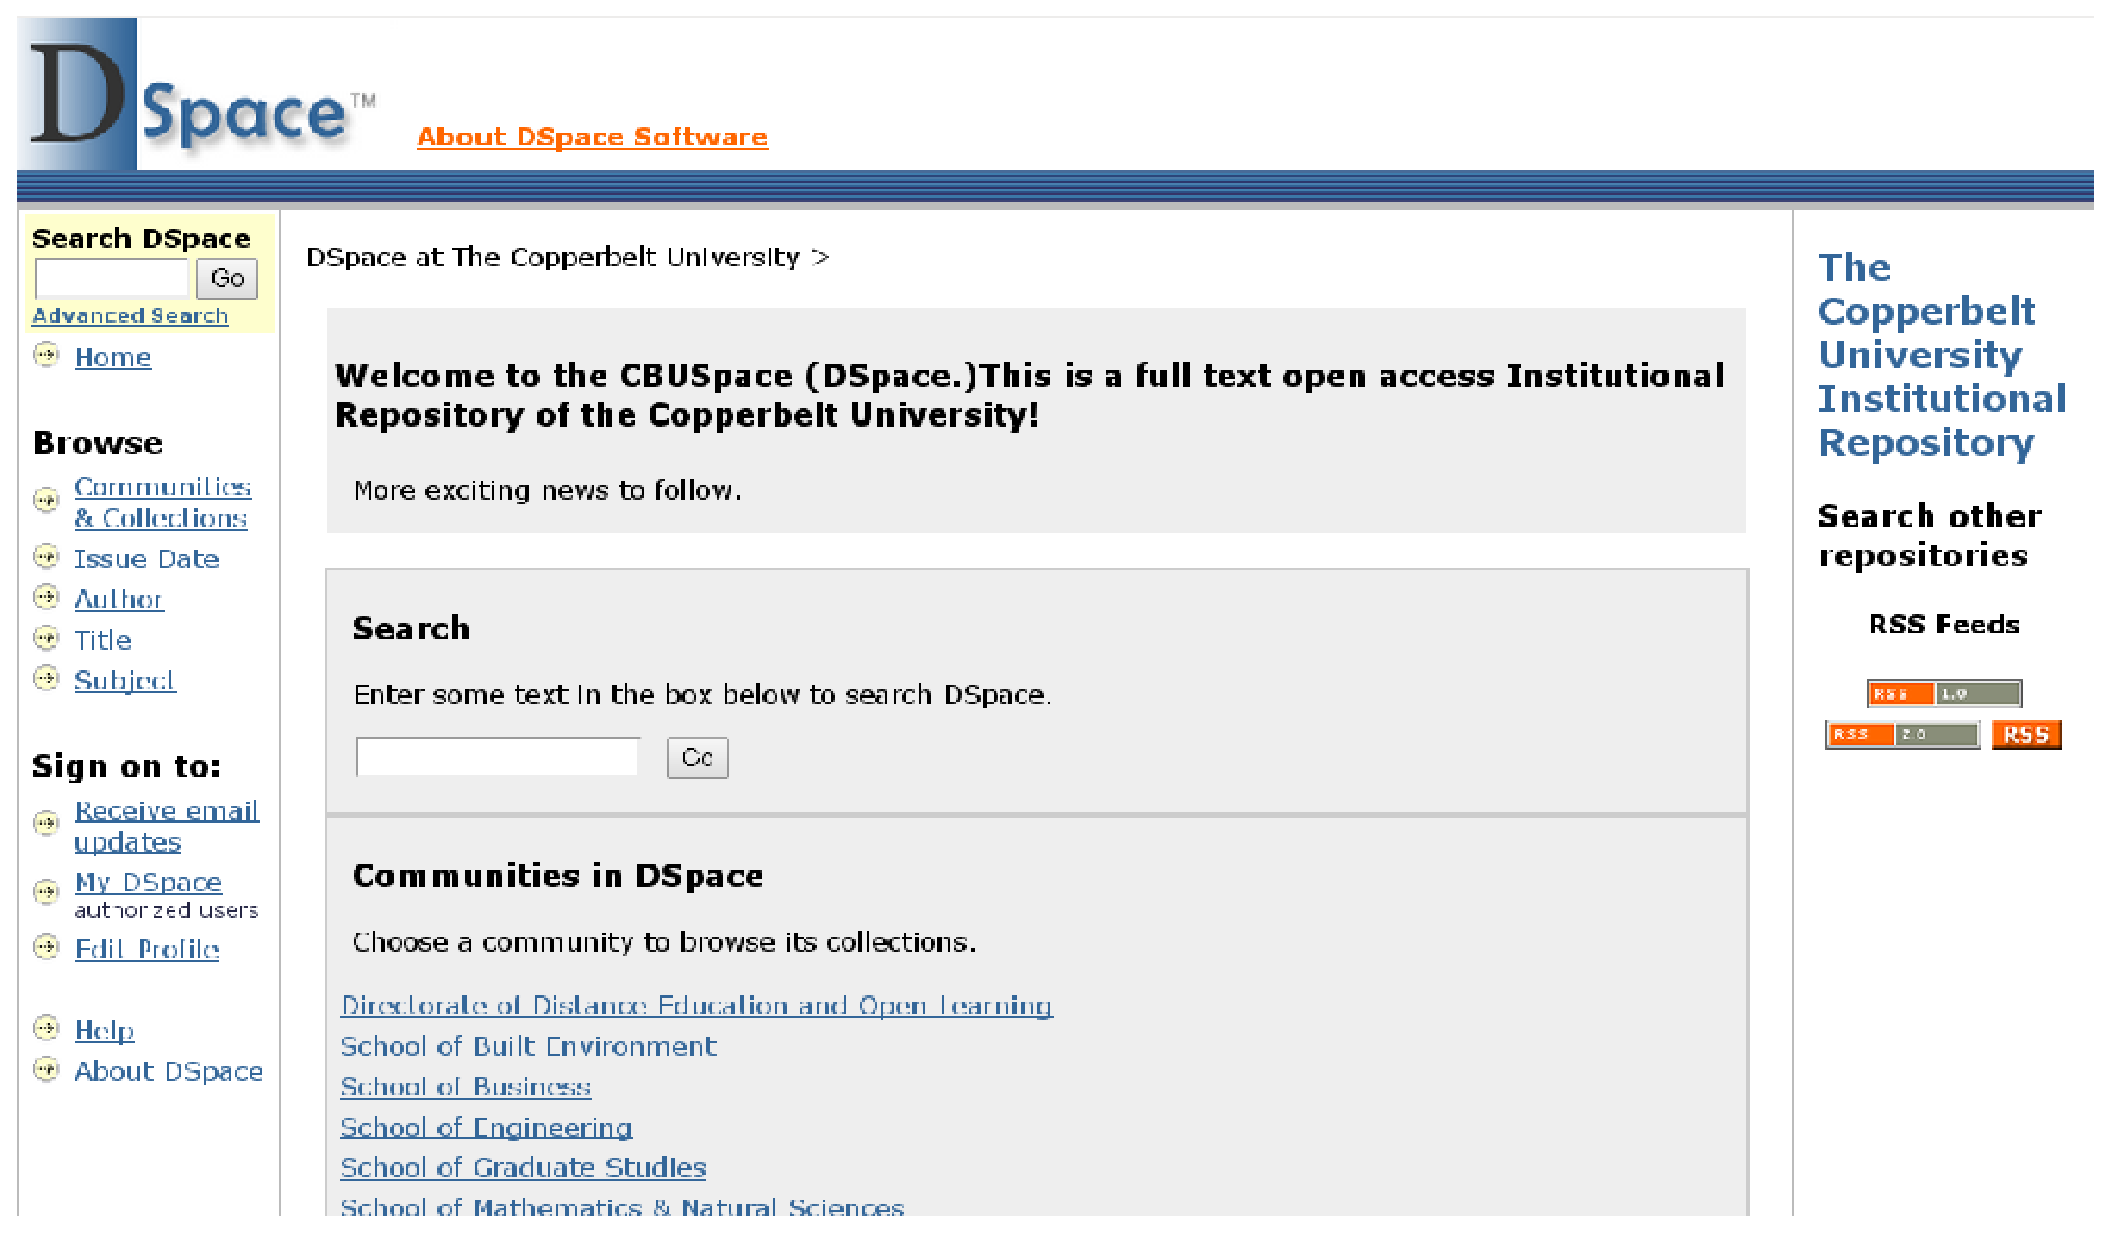
\includegraphics[width=0.95\textwidth]{chapter02/figures/zm-cbu-repository.eps}
  }%
  \caption{Screenshot showing the Copperbelt University institution repository}
  \label{fig:background:digital-libraries:zm-cbu-repository}
 %\end{center}
\end{figure}

Cultural heritage organisations are increasingly digitising historical artifacts
in a quest to display them online to a much wider audience. In light of this,
\glspl{dls} \index{Digital Library System} are being developed to enable easy access to this
information. Figure~\ref{fig:background:digital-libraries:uct-digital-lloydbleekcollection} is a
screen snapshot of the Digital Bleek and Lloyd
Collection\footnote{\url{http://lloydbleekcollection.cs.uct.ac.za}}\index{Bleek\& Lloyd}, which is a
digital collection of historical artifacts that document the culture and
language of the \textbar Xam and !Kun groups of Bushman people of Southern
Africa.

\begin{figure}
 %\begin{center}
  \centering
  \framebox[\textwidth]{%
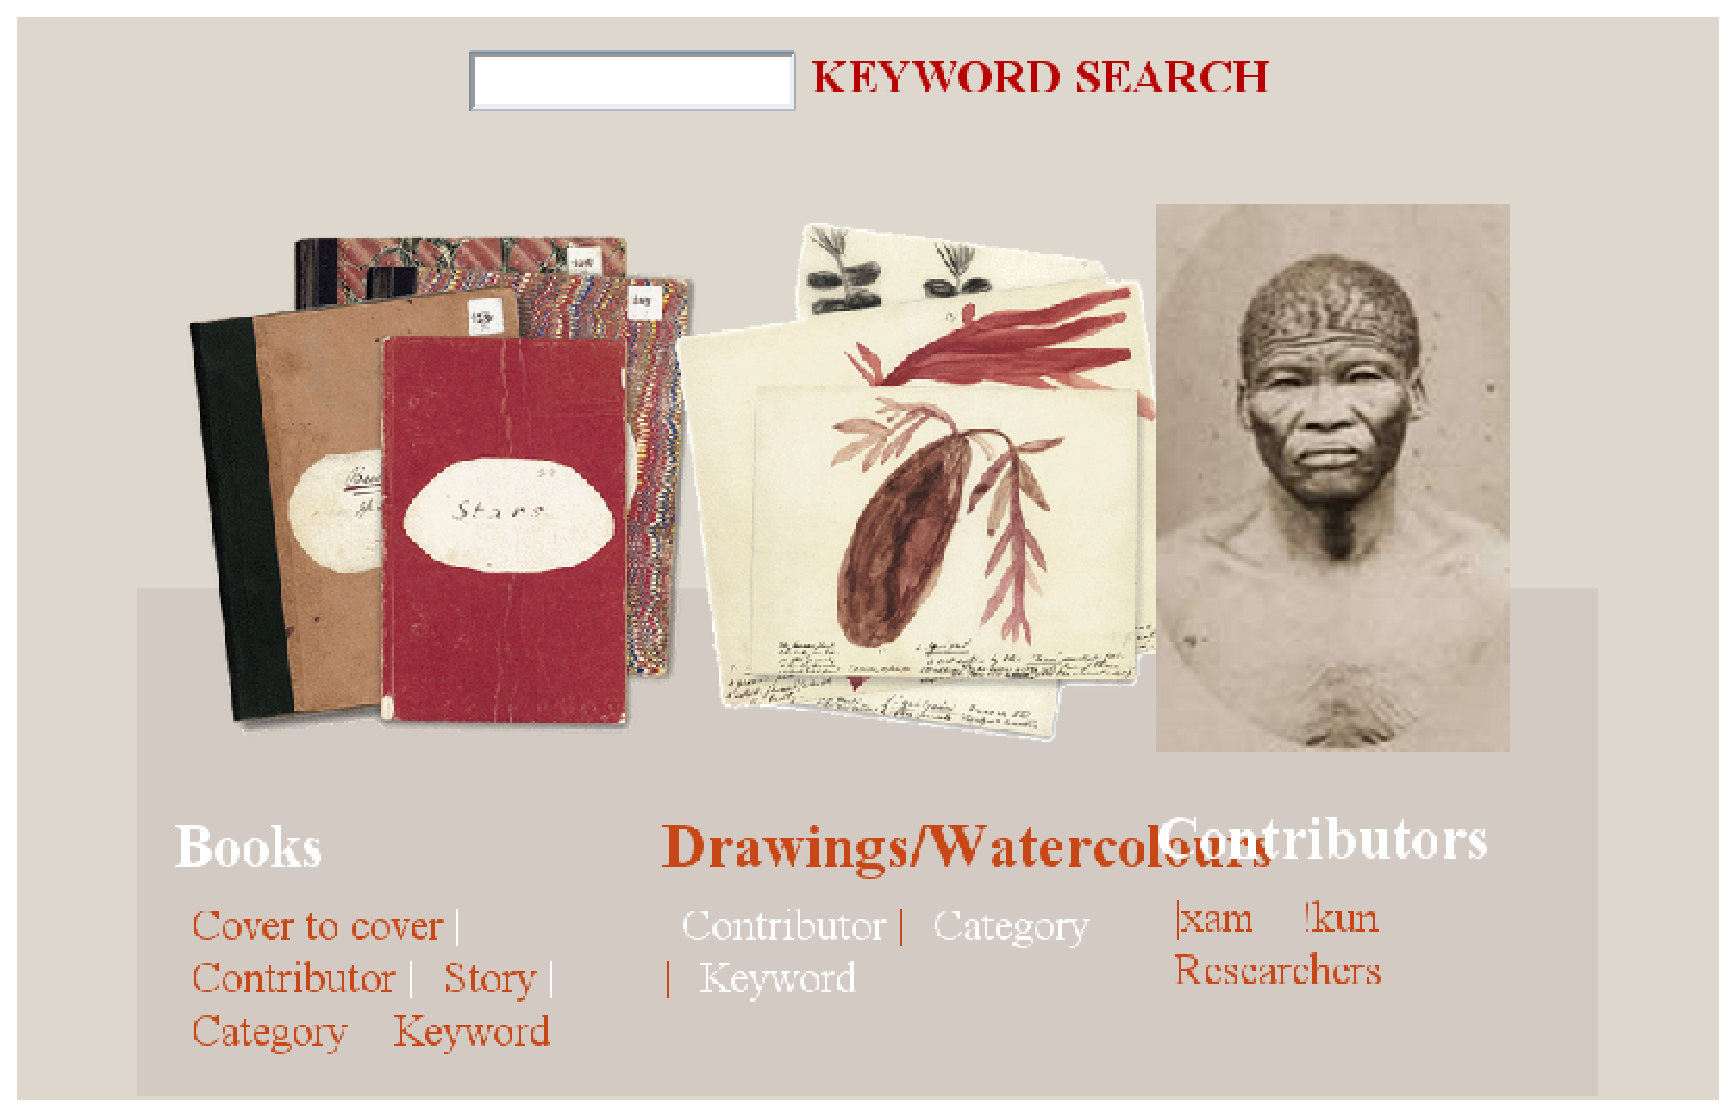
\includegraphics[width=0.95\textwidth]{%
chapter02/figures/uct-digital-lloydbleekcollection.eps}%
}%
\caption{Screenshot showing the digital Bleek\& Lloyd collection}
\label{fig:background:digital-libraries:uct-digital-lloydbleekcollection}
% \end{center}
\end{figure}


There has also been an increasing number of large scale archival projects that
have been initiated to preserve human knowledge and provide free access to vital
information \citep{Hart1992}.

\begin{figure}
 %\begin{center}
 \centering
  \framebox[\textwidth]{%
  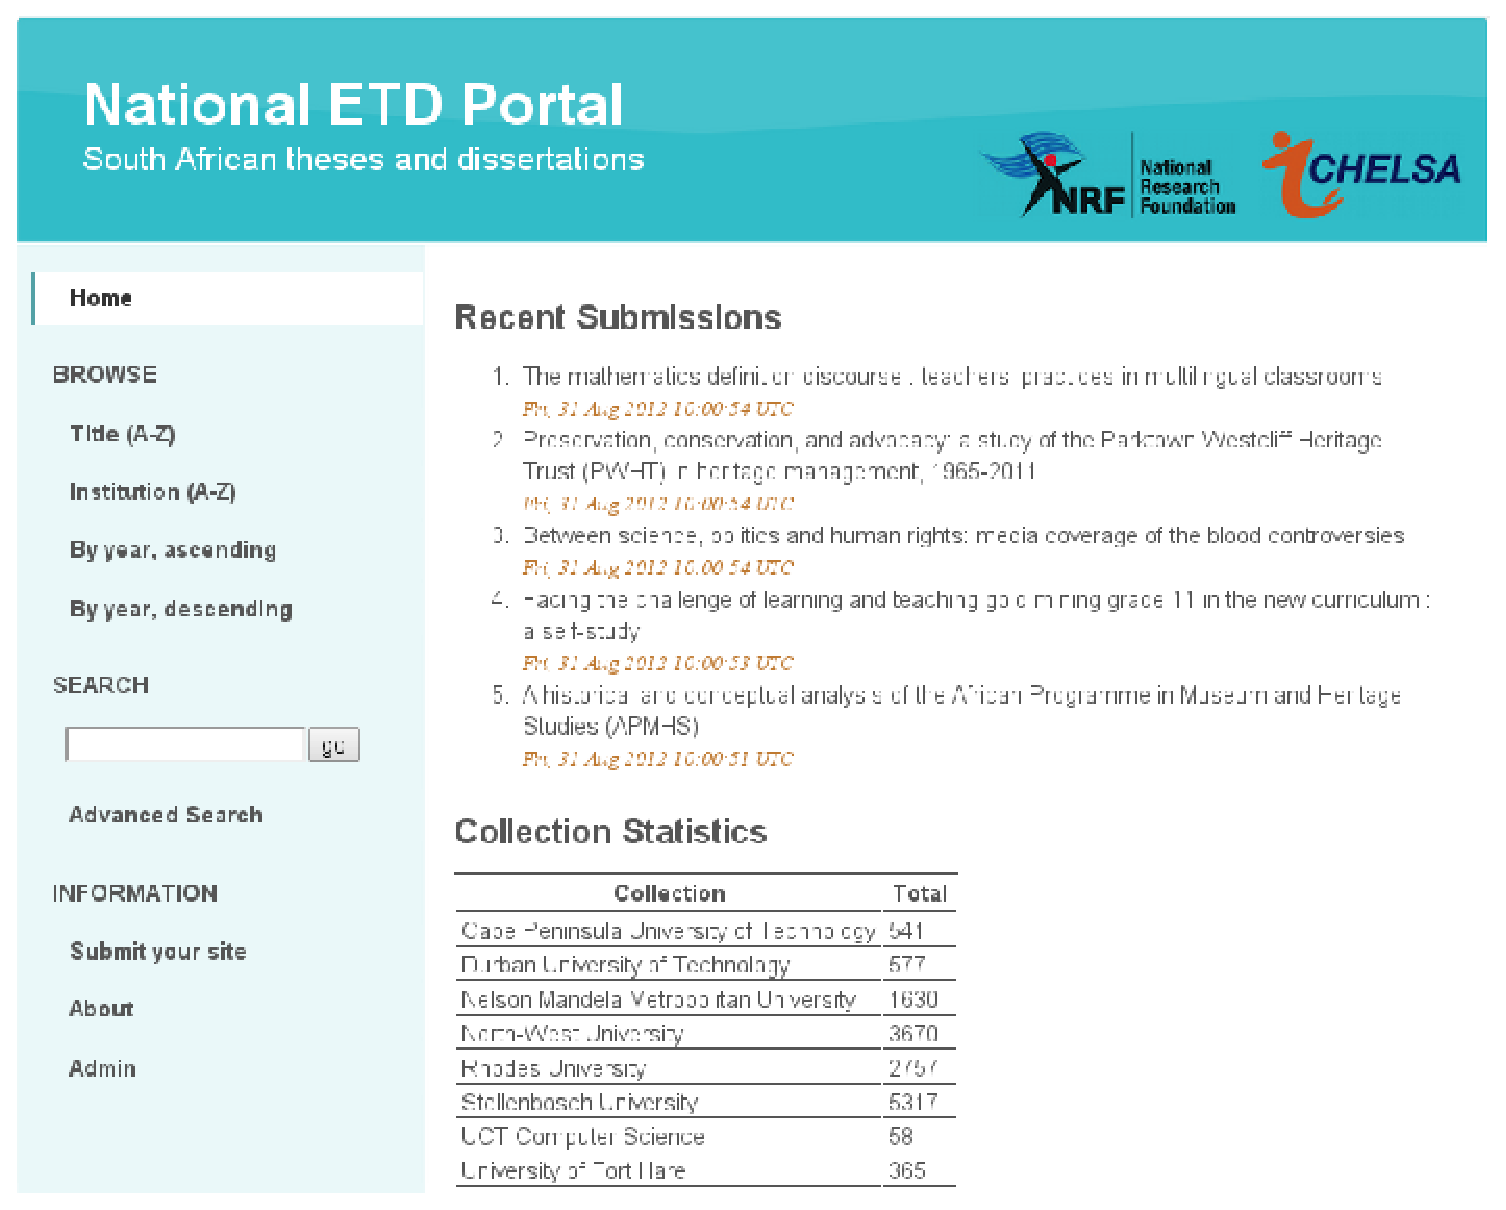
\includegraphics[width=0.95\textwidth]{chapter02/figures/sa-netd-portal.eps}
  }%
  \caption[Screenshot showing the South African NETD portal]{Screenshot showing the South African National Electronic Thesis and Dissertation portal}
  \label{fig:background:digital-libraries:sa-netd-portal}
 %\end{center}

\end{figure}

In addition, a number of federated services are increasingly being implemented
with the aim of making information from heterogeneous services available in
centralised location. Figure~\ref{fig:background:digital-libraries:sa-netd-portal} shows a snapshot of the
South African National Electronic Thesis and Dissertation (NETD) portal\index{NETD}---a federated
service that makes it possible for \glspl{etd}\index{ETD} from various South African universities
to be discovered from a central location.

\begin{figure}
 %\begin{center}
 \centering
  \framebox{%
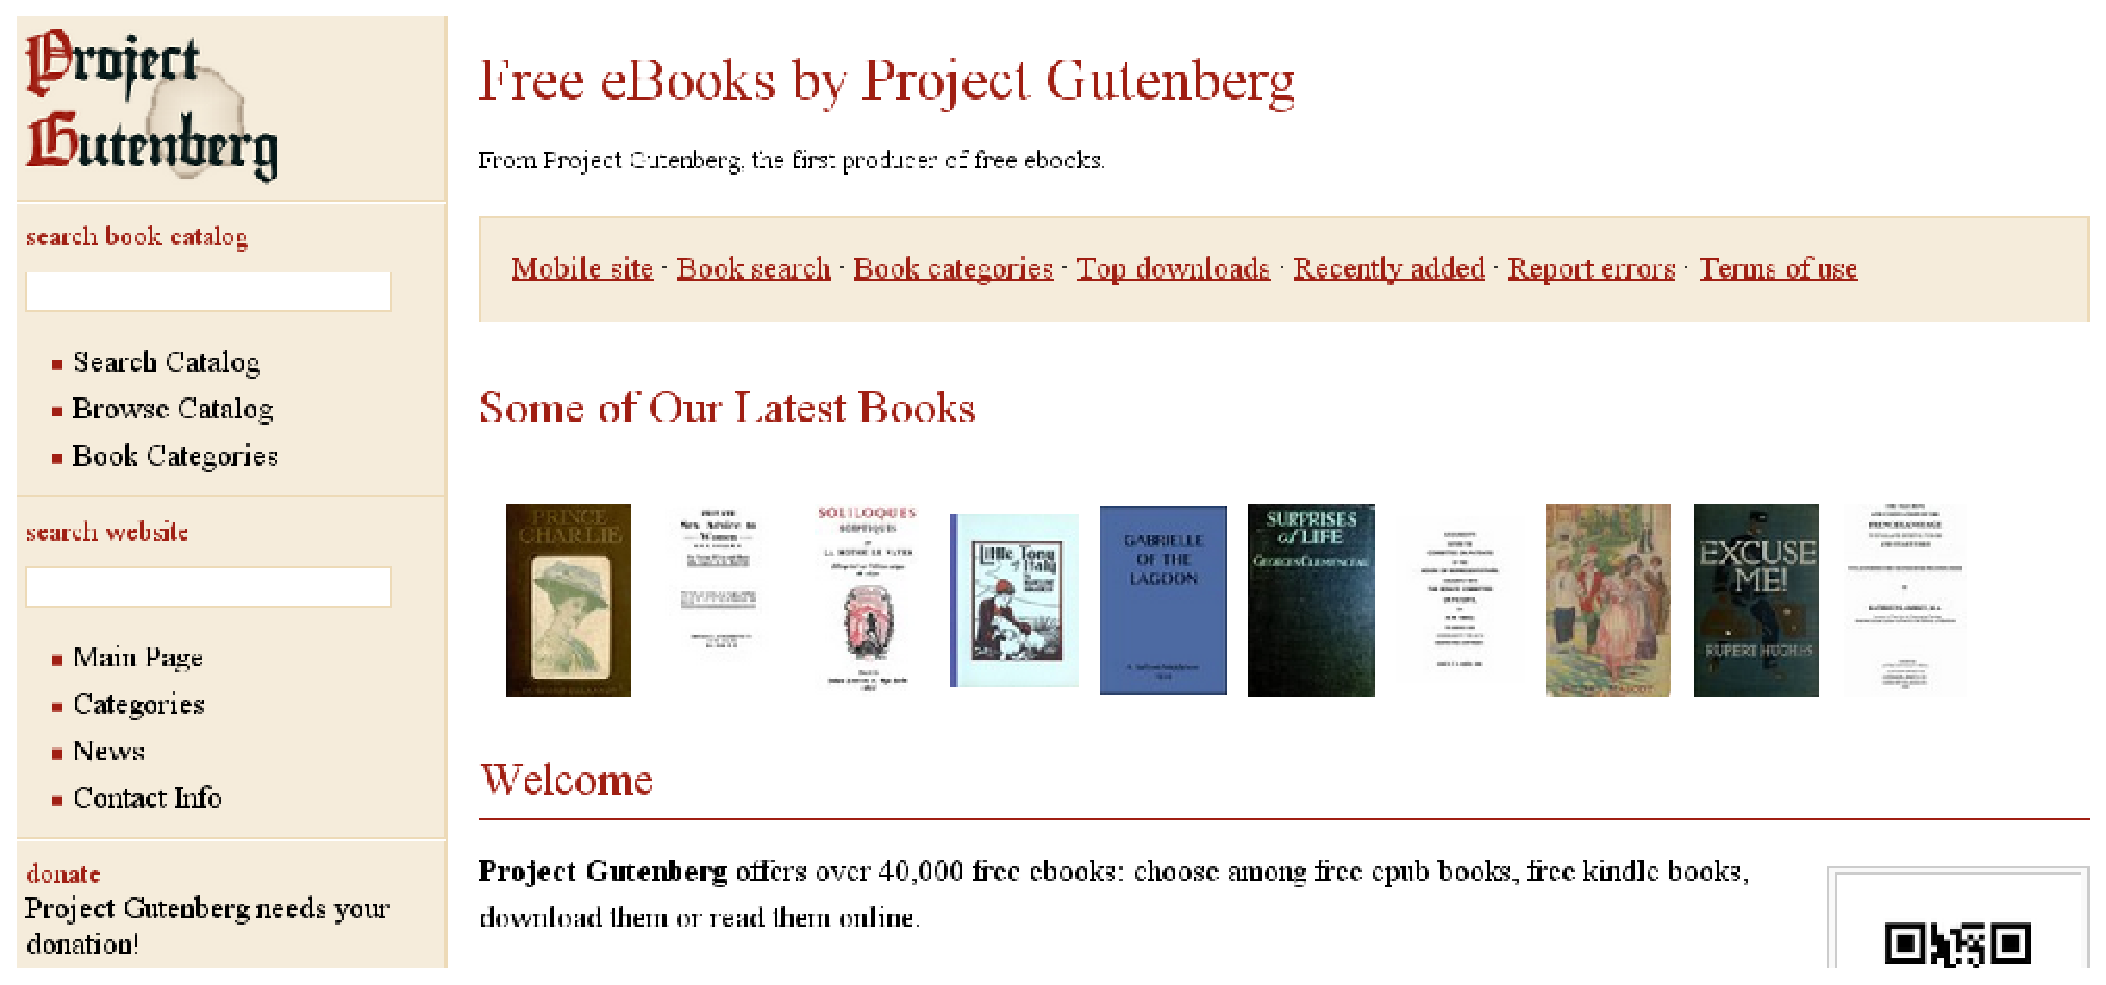
\includegraphics[width=0.95\textwidth]{chapter02/figures/project-gutenberg.eps}
  }%
  \caption{Screenshot showing the Project Gutenburg free ebooks portal}
  \label{fig:background:digital-libraries:project-gutenburg}
 %\end{center}
\end{figure}

\subsection{Summary}
\label{sec:background:digital-libraries:summary}

The massive number of physical copies being digitised, coupled with the increase in the generation of born-digital objects, has created a need for tools and services---\glspl{dl}---for making these objects easily accessible and preservable over long periods of time. The importance of these systems is manifested through their ubiquitous use in varying application domains.

This section broadly defined and described \glspl{dl}, and subsequently discussed some prominent application domains within which are currently used.
\section{Fundamental concepts}\index{Digital Libraries!Concepts}
\label{sec:background:fundamental-concepts}

\subsection{Identifiers}\index{Digital Libraries!Naming Schemes}
\label{sec:background:fundamental-concepts:identifiers}

An identifier is a name given to an entity for current and future reference. Arms \citep{Arms1995} classifies identifiers as vital building blocks for \gls{dl} \index{Digital Libraries} and emphasises their role in ensuring that individual digital objects are easily identified and changes related to the objects are linked to the appropriate objects. He also notes that they are also essential for information retrieval and for providing links between objects.

The importance of identifiers is made evident by the widespread adoption of standardised naming schemes such as \glspl{doi}\footnote{\url{http://www.doi.org}} \citep{Paskin2005,Paskin2010} \index{Digital Libraries!Naming Schemes!DOI}, Handles System\footnote{\url{http://www.handle.net}} and \glspl{purl}\footnote{\url{http://purl.oclc.org}}\index{Digital Libraries!Naming Schemes!PURL}.

\glspl{uri} \citep{RFC39862005} are considered a suitable naming scheme for digital objects primarily because they can potentially be resolved through standard Web protocols; that facilitates interoperability, a feature that is significant in \gls{dl} \index{Digital Libraries} whose overall goal is the widespread dissemination of information.

\subsection{Interoperability}\index{Digital Libraries!Interoperability}
\label{sec:background:fundamental-concepts:interoperability}

Interoperability\index{Interoperability} is a system attribute that enables a system to communicate and exchange information with other heterogeneous systems in a seamless manner. Interoperability\index{Interoperability} makes it possible for services, components and systems developed independently to potentially rely on one another to accomplish certain tasks with the overall goal of having individual components evolve independently, but be able to call on each other, thus exchanging information, efficiently and conveniently \citep{Paepcke1998}⁠. \gls{dl} interoperability has particularly made it possible for federated services \citep{Goncalves2001} to be developed, mainly due to the widespread use of the \gls{oaipmh}.

There are various protocols that have been developed to facilitate interoperability among heterogeneous \glspl{dls}. Prominent interoperability protocols include: Z39.50\index{Z39.50} \citep{Lynch1994}⁠ a client-server protocol used for remote searching; \gls{oaipmh}\index{OAI-PMH} \citep{Lagoze2002}⁠, which has been extensively used for metadata\index{Metadata} harvesting; and RSS\index{RSS} \citep{Winer2007}⁠, a Web based feed format commonly used for obtaining updates on Web resources.

\gls{xml} \index{XML} has emerged as the underlying language used to support a number of these interoperability protocols, largely due to its simplicity and platform independence.

\subsection{Metadata}\index{Digital Libraries!Metadata}
\label{sec:background:fundamental-concepts:metadata}

Metadata\index{Metadata} is representational information that includes pertinent descriptive annotations necessary to understand a resource. Arms \citep{Arms1997}⁠ describes different categories of information as being organised as sets of digital objects---a fundamental unit of the \gls{dl} architecture---that are composed of digital material and key-metadata. He defines the key-metadata as information needed to manage the digital object in a networked environment. The role performed by metadata\index{Metadata} is both implicit and explicit and its functions can be more broadly divided into distinct categories. A typical digital object normally has administrative metadata\index{Metadata} for managing the digital object, descriptive metadata\index{Metadata} to facilitate the discovery of information, structural metadata\index{Metadata} for describing relationships within  the digital object and preservation metadata\index{Metadata} that stores provenance information. Metadata\index{Metadata} is made up of elements that are grouped into a standard set, to achieve a specific purpose, resulting in a metadata\index{Metadata} schema. There are a number of metadata\index{Metadata} schemes that have been developed as standards across various disciplines and they include, among others, Dublin Core\index{Metadata!Schemes!Dublin Core} \citep{DCMI1999}⁠, Learning Object Metadata\index{Metadata} (LOM)\index{Metadata!Schemes!LOM} \citep{IEEE2002}, Metadata\index{Metadata} Encoding and Transmission Standard (METS)\footnote{\url{http://www.loc.gov/standards/mets}}\index{Metadata!Schemes!METS} and Metadata\index{Metadata} Object Description Schema (MODS)\footnote{\url{http://www.loc.gov/standards/mods}}\index{Metadata!Schemes!MODS}⁠. Metadata\index{Metadata} can either be embedded within the digital object---as is the case with Portable Document Format (PDF)\index{PDF} and Hypertext Transfer Markup Language (HTML)\index{HTML} documents---or stored separately with links to the resources being described. Metadata\index{Metadata} in \gls{dl} \index{Digital Libraries} is often stored in databases for easy management and access.

\subsection{Standards}\index{Digital Libraries!Concepts!Standards}
\label{sec:background:fundamental-concepts:standards}

The fast pace at which technology is moving has spawned different types of application software tools. This means that the choice of which technology to use in any given instance differs, thus complicating the process of integrating application software with other heterogeneous software tools. Standards become particularly useful in such situations because they form the basis for developing interoperable tools and services. A standard is a specification---a formal statement of a data format or protocol---that is maintained and endorsed by a recognised standards body \citep[see][chap. 2]{Suleman2010}⁠.

Adopting and adhering to standards has many other added benefits---and Strand et al. \citep{Strand1994} observe that applications that are built on standards are more readily scalable, interoperable and portable, constituting software quality attributes that are important for the design, implementation and maintenance of \glspl{dl}. Standards also play a vital role in facilitating long term preservation of digital objects by ensuring that documents still become easily accessible in the future. This is done by ensuring that the standard itself does not change and by making the standard backwards compatible. Notable use of standards in \gls{dl} \index{Digital Libraries} include the use of \gls{xml}\index{XML} as the underlying format for metadata\index{Metadata} and \gls{oaipmh}\index{OAI-PMH} as an interoperability protocol. Digital content is also stored in well known standards, as is the case with documents that are normally stored in \gls{pdfa}\index{OAI-PMH} format. The use of standards in \glspl{dls}, however, has its own shortcomings; in certain instances, the use of standards can be a very expensive venture as it may involve a lot of cross-domain effort \citep{Lorist2001}⁠.

\subsection{Summary}
\label{sec:background:fundamental-concepts:summary}

A \gls{dls} operates as a specialised type of information system and exhibits certain characteristics to attain its objects. This section discussed fundamental concepts, associated to \glspl{dls}, that help form the necessary building blocks for implementing \glspl{dl}.
\section[Frameworks]{Digital Libraries frameworks}\index{Digital Libraries!Frameworks}
\label{sec:background:reference-models-frameworks}

A reference model is an abstract framework that provides basic concepts used to understand the relationships among items in an environment. The \gls{oasis} \citep{MacKenzie2006}⁠ states that a reference model consists of a minimal set of unifying concepts, axioms and relationships within a particular problem domain, and is independent of specific standards, technologies, implementations or other concrete details.

Several \gls{dl} frameworks \citep{Gonccalves2004,Kahn2006} and reference models \citep{Candela2007a} have addressed specific problems in \gls{dls} architectural design and implementation. A discussion of some prominent reference models now follows.

%\subsection{Warwick Framework}
%\label{sec:background:reference-models-frameworks:warwick}
%
%Xxx xxx
%
%Xxx xxx
% @comment: Clearly, this right here is not in anyway relevant.
%
\subsection[5S framework]{Streams, Structures, Spaces and Societies}
\label{sec:background:reference-models-frameworks:5s}

The \gls{5s} framework\index{Digital Libraries!Frameworks!5S} is a unified formal theory for \glspl{dl}. It is an attempt to define and easily understand the complex nature of \glspl{dl} in a rigorous manner. The framework is based on formal definitions, and abstraction of five fundamental concepts---Streams, Structures, Spaces, Scenarios and Societies \citep{Gonccalves2004}⁠.  The five concepts, together with their corresponding definitions and examples, are summarised in Table~\ref{tab:background:reference-models-frameworks:5s}.

\tablespacing
%%%%%\begin{longtable}{p{0.15\linewidth} p{0.40\linewidth} p{0.30\linewidth}}
\begin{longtable}{
>{\arraybackslash}p{0.15\linewidth}|
>{\arraybackslash}p{0.40\linewidth}|
>{\arraybackslash}p{0.30\linewidth}}

\caption{Summary of key aspects of the 5S framework}
\label{tab:background:reference-models-frameworks:5s} \\
 %%%%%\toprule
 %%%%%\hline
 \textbf{Concept} & \textbf{Description} & \textbf{Examples} \\
 %%%%%\midrule
 \cline{1-3}
 \endfirsthead
 
 \caption[]{(continued)}\\
 %%%%%\toprule
 %%%%%\hline
 \textbf{Concept} & \textbf{Description} & \textbf{Examples} \\
 %%%%%\midrule
 \cline{1-3}
 \endhead
 
 % Page footer
 %%%%%\midrule
 %%%%%\hline
 \multicolumn{3}{r}{(Continued on next page)} \\
 \endfoot
 
 % Last page footer
 %%%%%\bottomrule
 \endlastfoot
 
 \textbf{Streams} &
 {Streams represent a sequence of elements of an arbitrary type} &
 {Text, video, audio, software} \\
 
 \cline{1-3}
 %\cmidrule[0.1pt](l{0.5em}r{0.5em}){1-3}
 
 \textbf{Structures} &
 {Structures specify the organisation of different parts of a whole} &
 {Collection, document, metadata} \\
 
 \cline{1-3}
 %\cmidrule[0.1pt](l{0.5em}r{0.5em}){1-3}
 
 \textbf{Spaces} &
 {Spaces are sets of objects, with associated operations, that obey certain constants} &
 {User interface, index} \\
 
 \cline{1-3}
 %\cmidrule[0.1pt](l{0.5em}r{0.5em}){1-3}
 
 \textbf{Scenarios} &
 {Scenarios define details for the behaviour of services} &
 {Service, event, action} \\
 
 \cline{1-3}
 %\cmidrule[0.1pt](l{0.5em}r{0.5em}){1-3}
 
 \textbf{Societies} &
 {Societies represent sets of entities and the relationships among them} &
 {Community, actors, relationships, attributes, operations} \\
 
\end{longtable}

\bodyspacing

In the context of the aims of \glspl{dl}, Gon\c{c}alves et al. \citep{Gonccalves2004} outline an association between \gls{5s} and some aims of a \gls{dls}, with Streams being aligned with the overall communication and consumption of information by end users; Structures supporting the organisation of information; Spaces dealing with the presentation and access to information in usable and effective ways; Scenarios providing the necessary support for defining and designing services; and Societies defining how a \gls{dl} satisfies the overall information needs of end users.

However, Candela et al. \citep{Candela2007}⁠ state that the \gls{5s} framework is very general-purpose and thus less immediate. The \gls{5s} framework is also arguably aimed at formalising the \gls{dl} aspects, as opposed to prescribing specific design guidelines.

\subsection[Kahn\& Wilensky framework]{Kahn and Wilensky framework}
\label{sec:background:reference-models-frameworks:kahn-wilensky}

This is a generic information system framework for distributed digital object services with digital objects as the main building blocks. The framework is based on an open architecture that supports large and distributed digital information services. Kahn and Wilensky\index{Digital Libraries!Frameworks!Kahn/Wilensky} \citep{Kahn2006}⁠ describe the framework in terms of the fundamental aspects of an open and distributed infrastructure, and how the basic components in such an infrastructure support storage, accessibility and management of digital objects.

In addition to a high level conceptual description of such a distributed information system, the framework primarily focuses on the network-based aspects of such an infrastructure \citep{Kahn2006}. Specifically, an elaborate description of how digital objects should be accessed via a \gls{rap} is outlined. The framework also proposes the use of a handle server infrastructure as a means for mapping registered digital objects.

In essence, the framework merely prescribes conventional methods for the unique identification, reliable location, and flexible access to digital objects.

\subsection{DELOS reference model}
\label{sec:background:reference-models-frameworks:delos}

The DELOS\index{Digital Libraries!Frameworks!DELOS} Network of Excellence on \glspl{dl}\footnote{\url{http://www.delos.info}} was a European Union co-funded project aimed at integrating and coordinating research activities in \glspl{dl}. The DELOS working group published a manifesto that establishes principles that facilitate the capture of the full spectrum of concepts that play a role in \glspl{dl} \citep{Candela2007a}⁠. The result of this project was a reference model---the DELOS \gls{dl} reference model---comprising to a set of concepts and relationships that collectively attempt to capture various entities of the \gls{dl} universe.

A fundamental part of the DELOS reference model is the \gls{dl} Manifesto, that presents a \gls{dl} as a three-tier framework consisting of a \gls{dl}, representing an organisation; a \gls{dls}, for implementing \gls{dl} services; and a \gls{dlms}, comprising of tools for administering the \gls{dls}. Figure~\ref{fig:background:reference-models-frameworks:delos}\footnote{Permission to reproduce this image was granted by Donatella Castelli} shows the interaction among the three sub-systems.

The reference model further identifies six core concepts that provide a firm foundation for \glspl{dl}. These six concepts---Content, User, Functionality, Quality, Policy and Architecture---are enshrined within the \gls{dl} and the \gls{dls}. All concepts, with the exceptions of the Architecture concept, appear in the definition of the \gls{dl}. The Architecture is, however, handled by the \gls{dls} definition \citep{Candela2007}⁠.

The Architecture component, addressed by the \gls{dls}, is particularly important in the context of this research as it represents the mapping of the functionality and content on to the hardware and software components. Candela et al. \citep{Candela2007}⁠ attribute the inherent complexity of \glspl{dl} and the interoperability challenges across \glspl{dl} as the two primary reasons for having Architecture as a core component.

Another important aspect of the reference model, directly related to this research, are the reference frameworks needed to clarify the \gls{dl} universe at different levels of abstraction. The three reference development frameworks are: Reference Model, Reference Architecture, and Concrete Architecture. In the context of architectural design, the Reference Architecture is vital as it provides a starting point for the development of an architectural design pattern, thus paving the way for an abstract solution.

\begin{figure}
 %\begin{center}
  \centering
  \framebox[\textwidth]{%
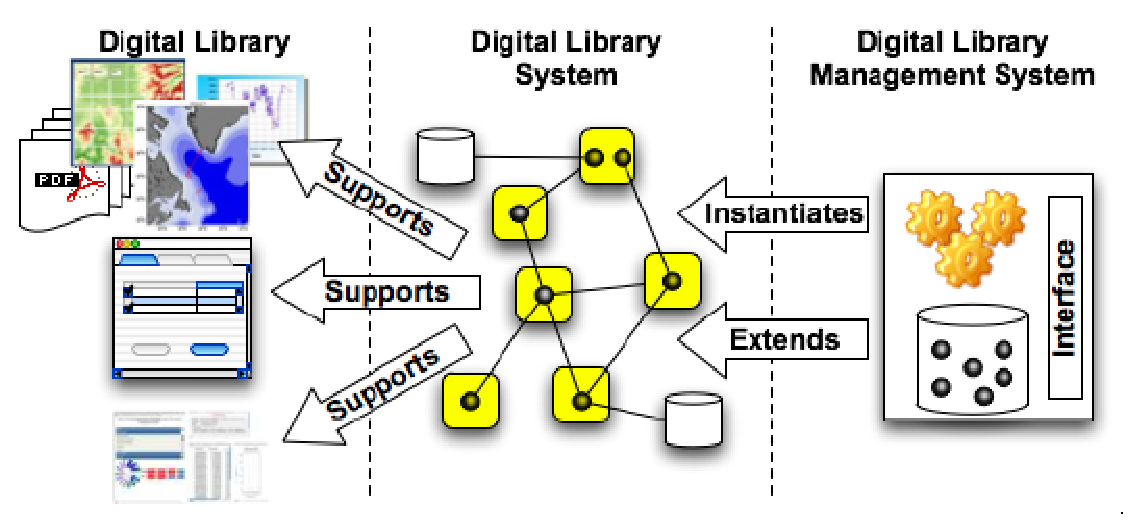
\includegraphics[width=0.95\textwidth]{%
chapter02/figures/delos-dl-dls-dlms.eps}%
}%
\caption[DL, DLS and DLMS: A three-tier framework]{DL, DLS and DLMS: A three-tier framework}
\label{fig:background:reference-models-frameworks:delos}
% \end{center}
\end{figure}

\subsection{Summary}
\label{sec:background:reference-models-frameworks:summary}

The motivation behind building both the reference models was largely influenced by the need to understand the complexity inherent in \glspl{dl}. The idea of designing a \gls{dl} architecture based on direct user needs is not taken into account in existing reference models, although the DELOS Reference Architecture does have a provision for the development of specific architectural design patterns. The DELOS Reference Architecture is in actual fact considered to be mandatory for the development of good quality \glspl{dls}, and for the integration and reuse of the system components.
\section[Software platforms]{Software platforms}\index{Digital Libraries!Software}
\label{sec:background:digital-libraries-software}

There are a number of different \gls{dl} software tools currently available. The ubiquitous availability of these tools could, in part, be as a result of specialised problems that these solutions are designed to solve. This section discusses seven prominent \gls{dl} software platforms.

\subsection{CDS Invenio}

CDS Invenio\index{Digital Libraries!Software!CDS Invenio}, formally known as CDSware\index{CDSware}, is an open source repository software, developed at CERN\footnote{\url{http://www.cern.ch}} and originally designed to run the CERN document server\footnote{\url{http://cdsweb.cern.ch}}. CDS Invenio provides an application framework with necessary tools and services for building and managing a \gls{dl} \citep{Vesely2004}.

The ingested digital objects' metadata\index{Metadata} records are internally converted into a MARC\index{MARC} 21 ---MARCXML--- representation structure, while the actually fulltext bitstreams are automatically converted into PDF\index{PDF}. This ingested content is subsequently accessed by downstream services via OAI service providers, email alerts and search engines \citep{Pepe2005}.

The implementation is based on a modular architecture. It is implemented using the Python Programming language, runs within an Apache/Python\index{Python} Web application server, and makes use of a MySQL\index{MySQL} backend database server for storage of metadata\index{Metadata} records.

\subsection{DSpace}

DSpace\index{Digital Libraries!Software!DSpace} is an open-source repository software that was specifically designed for storage of digital research and institutional materials. The architectural design was largely influenced by the need for materials to be stored and accessed over long periods of time \citep{Transley2003}.

The digital object metadata\index{Metadata} records are encoded using qualified Dublin Core\index{Dublin Core}---to facilitate effective resource description. Digital objects are accessed and managed via application layer services that support protocols such as OAI-PMH\index{OAI-PMH}.

DSpace\index{DSpace} is organised into a three-tier architecture, composed of: an application layer; a business logic layer; and a storage layer. The storage layer stores digital content within an asset store---a designated area within the operating system's filesystem; or can alternatively use a storage resource broker. The digital objects ---bitstreams\index{Bitstream} and corresponding metadata records--- are stored within a relational database management system \citep{Smith2003,Tansley2003a}. Furthermore software is implemented using the Java programming languages, and is thus deployed within a Servlet\index{Servlet} Engine. However, this architectural design approach arguably makes it difficult to recover digital objects in the event of a disaster since technical expertise would be required.

\subsection{EPrints}

EPrints\index{Digital Libraries!Software!EPrints} is an archival software that designed to create highly configurable Web-based archives. The initial design of the software can be traced back to a time when there was a need to foster open access to research publications, and provides a flexible \gls{dl} platform for building repositories \citep{Gutteridge2002}.

Eprints\index{EPrints} records are represented as data objects that contain metadata\index{Metadata}. The software's plugin architecture enables the flexible design and development of export plugins capable of converting repository objects into a variety of other formats. This technique effectively makes it possible for the data objects to be disseminated via different services---such as OAI data provider modules.

EPrints\index{EPrints} is implemented using Perl\index{Perl}, runs within an Apache HTTP\index{HTTP} server and uses a MySQL\index{MySQL} database server backend to store metadata records. However, the actual files in the archive are stored on the filesystem.

\subsection{ETD-db}

The ETD-db\index{Digital Libraries!Software!ETD-db} digital repository software for depositing, accessing and managing \gls{etd} collections. The software is more oriented towards helping facilitate the access and management of \glspl{etd}.

The software was initially developed as is a series of Web pages and additional Perl\index{Perl} scripts that interact with a MySQL\index{MySQL} database backend \citep{ETDdbHome}. However, the latest version---\gls{etd} 2.0---is a Web application, implemented using the Ruby on Rails Web application framework. This was done in an effort to handle \gls{etd} collections more reliably and securely. In addition, the latest version is able to work with any relational database and can be hosted on any Web server that supports Ruby on Rails \citep{Park2011}.

\subsection{Fedora Commons}

Fedora\index{Digital Libraries!Software!Fedora-Commons} is an open source digital content repository framework designed for managing and delivering complex digital objects \citep{Lagoze2006}.

The Fedora architecture is based on the Kahn and Wilensky framework \citep{Kahn2006}, discussed in Section~\ref{sec:background:reference-models-frameworks:kahn-wilensky}, with a distributed model that makes it possible for complex digital objects to make reference to content stored on remote storage systems. 

The Fedora framework is composed of loosely coupled services ---implemented using the Java programming language--- that interact with each other to provide the functionally of the Web service as a whole. The Web service functionalities are subsequently exposed via REST\index{REST} and SOAP\index{SOAP} interfaces.

\subsection{Greenstone}

Greenstone\index{Digital Libraries!Software!Greenstone} is an open source digital collection building and distributing software. The software's ability to redistribute digital collections on self-installing CD-ROMs has made it a popular tool of choice in regions with very limited bandwidth \citep{Witten2001}.

The most recent version---Greenstone3 \citep{Greenstone3}---is implemented in Java\index{Java}, making it platform independent. It was redesigned to improve the dynamic nature of the Greenstone toolkit and to further lower the potential overhead incurred by collection developers. In addition, it is distributed and can thus be spread across different servers. Furthermore, the new architecture is modular, utilising independent agent modules that communicate using single message calls \citep{Bainbridge2004}.

Greenstone uses \gls{xml}\index{XML} to encode resource metadata records ---XLinks\index{XLink} are used to represent relationships between other documents. Using this strategy, resources and documents are retrievable through \gls{xml}\index{XML} communication. Furthermore, indexing documents enables effective searching and browsing of resources. 

The software operates within an Apache Tomcat Servlet Engine.

\subsection{Omeka}

Omeka\index{Digital Libraries!Software!Omeka} is a Web-based publishing platform for publishing digital archives and collections \citep{Kucsma2010}. It is standards-based and highly interoperable---it makes use of unqualified Dublin Core and is \gls{oaipmh} compliant. In addition, it is relatively easy to use and has a very flexible design, which is customisable and highly extensible via the use of plugins.

Omeka is implemented using the PHP\index{PHP} scripting language and uses MySQL\index{MySQL} database as a backend for storage of metadata\index{Metadata} records. However, the ingested resources---bitstreams--- are stored on the filesystem.

\subsection{Summary}

Table~\ref{tab:background:related-work:digital-libraries-software:floss-matrix} is a feature matrix of the digital libraries software discussed in this section.

\tablespacing
%%%\begin{longtable}{p{0.03\linewidth} p{0.30\linewidth} p{0.03\linewidth}
%%%p{0.03\linewidth} p{0.03\linewidth} p{0.03\linewidth} p{0.03\linewidth}
%%%p{0.03\linewidth} p{0.03\linewidth}}
\begin{longtable}{
>{\centering\arraybackslash}p{0.008\linewidth}|
>{\arraybackslash}p{0.55\linewidth}|
>{\centering\arraybackslash}p{0.005\linewidth}|
>{\centering\arraybackslash}p{0.005\linewidth}|
>{\centering\arraybackslash}p{0.005\linewidth}|
>{\centering\arraybackslash}p{0.005\linewidth}|
>{\centering\arraybackslash}p{0.005\linewidth}|
>{\centering\arraybackslash}p{0.005\linewidth}|
>{\centering\arraybackslash}p{0.005\linewidth}
}
 
\caption{Feature matrix for some popular DL FLOSS software tools}
\label{tab:background:related-work:digital-libraries-software:floss-matrix} \\
 %%%%%\toprule
 %%%%%\cline{3-9}
 \multicolumn{1}{c}{} & 
 \multicolumn{1}{c|}{} & 
 \multicolumn{1}{c|}{\begin{sideways}\textbf{CDS Invenio}\end{sideways}} &
 \multicolumn{1}{c|}{\begin{sideways}\textbf{DSpace}\end{sideways}} &
 \multicolumn{1}{c|}{\begin{sideways}\textbf{EPrints}\end{sideways}} &
 \multicolumn{1}{c|}{\begin{sideways}\textbf{ETD-db}\end{sideways}} &
 \multicolumn{1}{c|}{\begin{sideways}\textbf{Fedora Commons}\end{sideways}} &
 \multicolumn{1}{c|}{\begin{sideways}\textbf{Greenstone}\end{sideways}} &
 \multicolumn{1}{c}{\begin{sideways}\textbf{Omeka}\end{sideways}} \\
 %%%%%\midrule
 \cline{1-9}
 \endfirsthead
 
 \caption[]{(continued)}\\
 %%%%%\toprule
 %%%%%\cline{3-9}
 \multicolumn{1}{c}{} & 
 \multicolumn{1}{c|}{} & 
 \multicolumn{1}{c|}{\begin{sideways}\textbf{CDS Invenio}\end{sideways}} &
 \multicolumn{1}{c|}{\begin{sideways}\textbf{DSpace}\end{sideways}} &
 \multicolumn{1}{c|}{\begin{sideways}\textbf{EPrints}\end{sideways}} &
 \multicolumn{1}{c|}{\begin{sideways}\textbf{ETD-db}\end{sideways}} &
 \multicolumn{1}{c|}{\begin{sideways}\textbf{Fedora Commons}\end{sideways}} &
 \multicolumn{1}{c|}{\begin{sideways}\textbf{Greenstone}\end{sideways}} &
 \multicolumn{1}{c}{\begin{sideways}\textbf{Omeka}\end{sideways}} \\
 \cline{1-9}
 \endhead
 
 % Page footer
 %%%%%\midrule
 \cline{1-9}
 \multicolumn{9}{c}{(Continued on next page)} \\
 \endfoot
 
 % Last page footer
 %%%%%\bottomrule
 \endlastfoot
 
 \multirow{6}{*}{\begin{sideways}\textbf{Storage} \end{sideways}} &
 \textbf{Complex object support}&
 {}&
 {}&
 {}&
 {}&
 {X}&
 {}&
 {}\\
 
 %%%%%\cmidrule[0.1pt](l{0.5em}r{0.5em}){2-9}
 \cline{3-9}
 
 &
 \textbf{Dublin Core support for metadata} &
 {}&
 {X}&
 {X}&
 {}&
 {X}&
 {X}&
 {X}\\
 
 %%%%%\cmidrule[0.1pt](l{0.5em}r{0.5em}){2-9}
 \cline{3-9}
  
 &
 \textbf{Metadata is stored in database} &
 {X}&
 {X}&
 {X}&
 {X}&
 {X}&
 {X}&
 {X}\\
 
 %%%%%\cmidrule[0.1pt](l{0.5em}r{0.5em}){2-9}
 \cline{3-9}
 
 {} &
 %%%%%\begin{sideways}\textbf{} \end{sideways} &
 \textbf{Metadata can be stored on filesystem} &
 {}&
 {}&
 {}&
 {}&
 {}&
 {X}&
 {}\\
 
 %%%%%\cmidrule[0.1pt](l{0.5em}r{0.5em}){2-9}
 \cline{3-9}
 
  &
 \textbf{Supports distributed repositories} &
 {X}&
 {X}&
 {X}&
 {X}&
 {X}&
 {X}&
 {X}\\
 
 %%%%%\cmidrule[0.1pt](l{0.5em}r{0.5em}){2-9}
 \cline{1-9}
 
  &
 \textbf{Object relationship support} &
 {}&
 {}&
 {}&
 {}&
 {X}&
 {}&
 {X}\\
 
 %%%%%\cmidrule[0.1pt](l{0.5em}r{0.5em}){1-9}
 \cline{3-9}
 
 \multirow{5}{*}{\begin{sideways}\textbf{Services} \end{sideways}} &
 \textbf{Extensible via plugins} &
 {X}&
 {X}&
 {X}&
 {}&
 {X}&
 {X}&
 {X}\\
 
 %%%%%\cmidrule[0.1pt](l{0.5em}r{0.5em}){2-9}
 \cline{3-9}
 
  &
 \textbf{OAI-PMH complaint} &
 {X}&
 {X}&
 {X}&
 {X}&
 {X}&
 {X}&
 {X}\\
 
 %%%%%\cmidrule[0.1pt](l{0.5em}r{0.5em}){2-9}
 \cline{3-9}
  
 %\begin{sideways}\textbf{Technologies}\end{sideways} &
 \begin{sideways}\textbf{}\end{sideways} &
 \textbf{Platform independent} &
 {}&
 {X}&
 {X}&
 {}&
 {X}&
 {X}&
 {X}\\
 
 %%%%%\cmidrule[0.1pt](l{0.5em}r{0.5em}){2-9}
 \cline{3-9}
  
  &
 \textbf{Supports Web services} &
 {}&
 {X}&
 {}&
 {}&
 {X}&
 {X}&
 {}\\
 
 %%%%%\cmidrule[0.1pt](l{0.5em}r{0.5em}){2-9}
 \cline{3-9}
  
  &
 \textbf{URI support(e.g. DOIs)} &
 {}&
 {X}&
 {}&
 {}&
 {X}&
 {}&
 {}\\
 
 %%%%%\cmidrule[0.1pt](l{0.5em}r{0.5em}){2-9}%
 \cline{1-9}
 
 \multirow{7}{*}{\begin{sideways}\textbf{Features} \end{sideways}} &
 \textbf{Alternate accessibility (e.g. CD-ROM)} &
 {}&
 {}&
 {}&
 {}&
 {}&
 {X}&
 {}\\
 
 %%%%%\cmidrule[0.1pt](l{0.5em}r{0.5em}){2-9}
 \cline{3-9}

   &
 \textbf{Easy to setup, configure and use} &
 {}&
 {}&
 {X}&
 {}&
 {}&
 {X}&
 {X}\\
 
 %%%%%\cmidrule[0.1pt](l{0.5em}r{0.5em}){2-9}
 \cline{3-9}
 
   &
 \textbf{Handles different file formats} &
 {X}&
 {X}&
 {X}&
 {}&
 {X}&
 {X}&
 {X}\\
 
 %%%%%\cmidrule[0.1pt](l{0.5em}r{0.5em}){1-9}
 \cline{3-9}
 
  &
 \textbf{Hierarchical collection structure} &
 {}&
 {X}&
 {X}&
 {}&
 {X}&
 {X}&
 {}\\
 
 %%%%%\cmidrule[0.1pt](l{0.5em}r{0.5em}){2-9}
 \cline{3-9}
 
 %\begin{sideways}\textbf{Features}\end{sideways} &
 \begin{sideways}\textbf{}\end{sideways} &
 \textbf{Horizontal market software} &
 {X}&
 {X}&
 {X}&
 {}&
 {X}&
 {X}&
 {X}\\

 %%%%%\cmidrule[0.1pt](l{0.5em}r{0.5em}){2-9}
 \cline{3-9}
 
   &
 \textbf{Web interface} &
 {X}&
 {X}&
 {X}&
 {X}&
 {X}&
 {X}&
 {X}\\
 
 %%%%%\cmidrule[0.1pt](l{0.5em}r{0.5em}){2-9}
 \cline{3-9}
 
   &
 \textbf{Workflow support} &
 {X}&
 {X}&
 {X}&
 {X}&
 {}&
 {}&
 {}\\
 
\end{longtable}

\bodyspacing
\section{Minimalist philosophy}\index{Minimalism}
\label{sec:background:simple-architectures}

The application of minimalism\index{Minimalism} in both software and hardware designs is widespread, and has been employed since the early stages of computing. The Unix\index{Unix} operating system is perhaps one prominent example that provides a unique case of the use of minimalism as a core design philosophy, and Raymond \citep{Raymond2004} outlines the benefits, on the Unix platform, of designing for simplicity\index{Simplicity}. This section discusses relevant architectures that were designed with simplicity\index{Simplicity} in mind.

% Not quite sure if this subsubsection is relevant---might have to figure out
% how to incorporate this information in a different section
%\subsection{Ubiquitous Access to Information}
%\label{sec:background:related-work:ubiquitous-access}
%Various solutions have been devised to facilitate ubiquitous access to
%knowledge by overcoming problems experienced in resource constrained
%environments.

%\subsubsection{One Laptop Per Child Project}
%\label{sec:background:related-work:ubiquitous-access}

%xxxx xxxx

%\subsection{World Wide Web}
%\label{sec:background:world-wide-web}
% NOT YET SURE ABOUT INCLUDING THE WEB HERE
%xxx xxx

\subsection[Dublin Core]{Dublin Core element set}
\label{sec:background:simple-architectures:dublin-core-element-set}

The Dublin Core\index{Dublin Core} metadata\index{Metadata} element set defines a set of 15 resource description properties that are potentially applicable to a wide range of resources. One of the main goals of the Dublin Core\index{Dublin Core} element set is aimed at keeping the element set as small and simple as possible to facilitate the creation of resource metadata by non-experts \citep{Hillmann2005}.

\tablespacing
%%%%%\begin{longtable}{p{0.15\linewidth} p{0.75\linewidth}}
\begin{longtable}{
>{\arraybackslash}p{0.16\linewidth}|
>{\arraybackslash}p{0.74\linewidth}}
 
 \caption{Simple unqualified Dublin Core element set}
\label{tab:background:simple-architectures:dublin-core-element-set} \\
 %%%%%\toprule
 %%%%%\hline
 \textbf{Element} & \textbf{Element Description}\\
 %%%%%\midrule
 \cline{1-2}
 \endfirsthead
 
 \caption[]{(continued)}\\
 %%%%%\toprule
 %%%%%\hline
 \textbf{Element} & \textbf{Element Description}\\
 %%%%%\midrule
 \cline{1-2}
 \endhead
 
 % Page footer
 %%%%%\midrule
 %%%%%\hline
 \multicolumn{2}{r}{(Continued on next page)} \\
 \endfoot
 
 % Last page footer
 %%%%%\bottomrule
 \endlastfoot
 
 \textbf{Contributor} &
 {An entity credited for making the resource available} \\
 
 \cline{1-2}
 %\cmidrule[0.1pt](l{0.5em}r{0.5em}){1-2}
 
 \textbf{Coverage} &
 {Location specific details associated to the resource} \\
 
 \cline{1-2}
 %\cmidrule[0.1pt](l{0.5em}r{0.5em}){1-2}
 
 \textbf{Creator} &
 {An entity responsible for creating the resource} \\
 
 \cline{1-2}
 %\cmidrule[0.1pt](l{0.5em}r{0.5em}){1-2}
 
 \textbf{Date} &
 {A time sequence associated with the resource life-cycle} \\

 \cline{1-2}
 %\cmidrule[0.1pt](l{0.5em}r{0.5em}){1-2}
 
 \textbf{Description} &
 {Additional descriptive information associated to the resource} \\

 \cline{1-2}
 %\cmidrule[0.1pt](l{0.5em}r{0.5em}){1-2}
 
 \textbf{Format} &
 {Format specific attributes associated with the resource} \\

 \cline{1-2}
 %\cmidrule[0.1pt](l{0.5em}r{0.5em}){1-2}
 
 \textbf{Identifier} &
 {A name used to reference the resource} \\

 \cline{1-2}
 %\cmidrule[0.1pt](l{0.5em}r{0.5em}){1-2}
 
 \textbf{Language} &
 {The language used to publish the resource} \\

 \cline{1-2}
 %\cmidrule[0.1pt](l{0.5em}r{0.5em}){1-2}
 
 \textbf{Publisher} &
 {An entity responsible for making the resource available} \\

 \cline{1-2}
 %\cmidrule[0.1pt](l{0.5em}r{0.5em}){1-2}

 \textbf{Relation} &
 {Other resource(s) associated with the resource} \\

 \cline{1-2}
 %\cmidrule[0.1pt](l{0.5em}r{0.5em}){1-2}
 
 \textbf{Rights} &
 {The access rights associated with the resource} \\

 \cline{1-2}
 %\cmidrule[0.1pt](l{0.5em}r{0.5em}){1-2}
 
 \textbf{Source} &
 {The corresponding resource where the resource is derived from} \\

 \cline{1-2}
 %\cmidrule[0.1pt](l{0.5em}r{0.5em}){1-2}
 
 \textbf{Subject} &
 {The topic associated to the resource} \\

 \cline{1-2}
 %\cmidrule[0.1pt](l{0.5em}r{0.5em}){1-2}
 
 \textbf{Title} &
 {The name of the resource} \\

 \cline{1-2}
 %\cmidrule[0.1pt](l{0.5em}r{0.5em}){1-2}
 
 \textbf{Types} &
 {The resource type} \\
 
\end{longtable}

\bodyspacing

The simplicity\index{Simplicity} of the element set arises from the fact that the 15 elements form the smallest possible set of elements required to describe a generic resource. In addition, as shown in Table~\ref{tab:background:simple-architectures:dublin-core-element-set}, the elements are self explanatory, effectively making it possible for a large section of most communities to make full use of the framework. Furthermore, all the elements are repeatable and at the same time optional. This flexibility of the scheme is, in part, the research why it is increasingly becoming popular.

\subsection[Wikis]{Wiki software}\index{Wiki}
\label{sec:background:simple-architectures:wiki-software}

Wiki software allows users to openly collaborate with each other through the process of creation and modification of Web page content \citep{Leuf2001}. The success of Wiki software is, in part, attributed to the growing need for collaborative Web publishing tools. However, the simplicity\index{Simplicity} in the way content is managed, to leverage speed, flexibility and easy of use, is arguably the major contributing factor to their continued success. The strong emphasis on simplicity\index{Simplicity} in the design of Wikis is evident in Cunningham's original description: ``The simplest online database that could possibly work'' \citep{Ward1995,Leuf2001}.

\subsection[XML]{Extensible markup language}
\label{sec:background:simple-architectures:extensible-markup-language}

\gls{xml}\index{XML} is a self-describing markup language that was specifically designed to transport and store data. \gls{xml} provides a hardware- and software-independent mode for carrying information, and was design for ease of use, implementation and interoperability from the onset. This is in fact evident from the original design goals that, in part, emphasised for the language to be easy to create documentations, easy to write programs for processing the documents and straightforwardly usable over the Internet \citep{Bray2008}.

\gls{xml} has become one of the most commonly used tool for transmission of data in various applications due to the following reasons.

\begin{itemize}
 \item Extensibility through the use of custom extensible tags
 \item Interoperability by being usable on a wide variety of hardware and software platforms
 \item Openness through the open and freely available standard
 \item Simplicity of resulting documents, effectively making them readable by machines and humans
\end{itemize}

The simplicity\index{Simplicity} of \gls{xml} particularly makes it an easy and flexible tool to work with, in part, due to the fact that the \gls{xml} document syntax is composed of a fairly minimal set of rules. Furthermore, the basic minimal set of rules can be expanded to grow more complex structures as the need arises.

\subsection[OAI-PMH]{OAI protocol for metadata harvesting}
\label{sec:background:oaipmh-protocol-for-metadata-harvesting}

The \gls{oaipmh} \index{OAI-PMH} is a metadata harvesting interoperability framework \citep{Lagoze2002}. The protocol only defines a set of six request verbs\index{OAI-PMH!Verbs}, shown in Table~\ref{tab:background:simple-architectures:oaipmh-request-verbs}, that data providers need to implement. Downstream service providers then harvest metadata as a basis for providing value-added services.

\tablespacing
%%%%%\begin{longtable}{p{0.30\linewidth} p{0.60\linewidth}}
\begin{longtable}{
>{\arraybackslash}p{0.30\linewidth}|
>{\arraybackslash}p{0.60\linewidth}}
 
 \caption{OAI-PMH request verbs}
\label{tab:background:simple-architectures:oaipmh-request-verbs} \\
 %%%%%\toprule
 %%%%%\hline
 \textbf{Request Verb} & \textbf{Description}\\
 %%%%%\midrule
 \cline{1-2}
 \endfirsthead
 
 \caption[]{(continued)}\\
 %%%%%\toprule
 %%%%%\hline
 \textbf{Request Verb} & \textbf{Description}\\
 %%%%%\midrule
 \cline{1-2}
 \endhead
 
 % Page footer
 %%%%%\midrule
 %%%%%\hline
 \multicolumn{2}{r}{(Continued on next page)} \\
 \endfoot
 
 % Last page footer
 %%%%%\bottomrule
 \endlastfoot

 \textbf{GetRecord} &
 {This verb facilitates retrieval of individual metadata records} \\

 \cline{1-2}
 %\cmidrule[0.1pt](l{0.5em}r{0.5em}){1-2}

 \textbf{Identify} &
 {This verb is used for the retrieval of general repository information} \\

 \cline{1-2}
 %\cmidrule[0.1pt](l{0.5em}r{0.5em}){1-2}
 
 \textbf{ListIdentifiers} &
 {This verb is used to harvest partial records in the form of record headers} \\
 
 \cline{1-2}
 %\cmidrule[0.1pt](l{0.5em}r{0.5em}){1-2}

 \textbf{ListMetadataFormats} &
 {This verb is used to retrieve metadata formats that are supported} \\

 \cline{1-2}
 %\cmidrule[0.1pt](l{0.5em}r{0.5em}){1-2}
 
 \textbf{ListRecords} &
 {This verb is used to harvest complete records} \\
 
 \cline{1-2}
 %\cmidrule[0.1pt](l{0.5em}r{0.5em}){1-2}
 
 \textbf{ListSets} &
 {This verb is used to retrieve the logical structure defined in the repository} \\
 
\end{longtable}

\bodyspacing

The \gls{oaipmh} framework was initially conceived to provide a low-barrier to interoperability with the aim of providing a solution that was easy to implement and deploy \citep{Lagoze2001}. The use of widely used and existing standards, in particular \gls{xml} and Dublin Core\index{Dublin Core} for encoding metadata records and HTTP\index{HTML} as the underlying transfer protocol, renders the protocol flexible to work with. It is increasingly being widely used as an interoperability protocol.

\subsection{Project Gutenberg}
\label{sec:background:related-work:project-gutenberg}

Project Gutenberg\footnote{\url{http://www.gutenberg.org}} is a pioneering initiative, aimed at encouraging the creation and distribution of eBooks, that was initiated in 1971 \citep{GutenbergAbout}. The project was the first single collection of free electronic books (eBooks) and its continued success is attributed to its philosophy \citep{Hart1992}, where minimalism is the overarching principle. This principle was adopted to ensure that the electronic texts were available in the simplest, easiest to use forms; independent of the software and hardware platforms used to access the texts.

\subsection{Summary}
\label{sec:background:simple-architectures:summary}

This section has outlined, through a discussion of some prominent design approaches, how simplicity\index{Simplicity} in architectural designs can be leveraged and result in more flexible systems that are subsequently easy to work with. In conclusion, the key to designing easy to use tools, in part, lies in identifying the least possible components that can result in a functional unit and subsequently add complexity, in the form of optional components, as need arises. Minimalist designs should not only aim to result in architectures that are easier to extend, but also easier to work with.
\section{Data storage schemes}
\label{sec:background:data-storage-architectures}

The repository sub-layer forms the core architectural component of a typical
digital library system and more specifically, it is composed of two components:
a bitstream\index{Bitstream} store and a metadata\index{Metadata} store, responsible for storing digital content
and metadata\index{Metadata} records respectively. As shown in Table~\ref{tab:background:related-work:digital-libraries-software:floss-matrix},
\glspl{dls} are generally implemented in such a manner that digital
content is stored on the file system, whilst the metadata\index{Metadata} records are almost
always housed in a relational database\index{RDMS}.

This section discusses three prominent data storage solutions that can
potentially be integrated within the repository sub-layer for metadata\index{Metadata} storage.
The focus is to assess their suitability for integration with
\glspl{dls}.

\subsection{Relational databases}
\label{sec:background:data-storage-architectures:relational-databases}

Relational databases\index{Storage Schemes!RDBMS} have stood the test of time, having been around for
decades. They have, until recently, been the preferred choice for data
storage. There are a number of reasons \citep[see][chap. 3]{Elmasri2008} why relational databases have proved to
be a popular storage solution, and these include:

\begin{itemize}
 \item The availability of a simple, but effective query language---SQL---
capable of retrieving multifaceted views of data
 \item Support for Data model relationships via table relations
 \item Transaction support through ACID\footnote{Atomicity, Consistency, Isolation, Durability} properties
 \item Support for data normalisation, thus preventing redundancy
\end{itemize}

Relational databases are, however, mostly suitable for problem domains
that require frequent retrieval and update of relatively small quantities of
data.

\subsection{NoSQL databases}
\label{sec:background:data-storage-architectures:nosql-databases}

The large-scale production of data \citep{Gantz2008}, coupled with the now
prevalent Big Data\footnote{\url{http://www-01.ibm.com/software/data/bigdata}},
has resulted in a profound need for data storage architectures that are
efficient, horizontally scalable, and easier to interface with. As a result,
NoSQL databases recently emerged as potential alternatives to relational
databases. NoSQL\index{Storage Schemes!NoSQL} databases are non-relational databases that embrace schemaless
data, are capable of running on clusters, and generally trade off consistency
for other properties such as performance \citep[see][chap.
1]{Sadalage2004}.

NoSQL database implementations are often categorised based on the manner in
which they store data, and typically fall under the categories described in
Table~\ref{tab:background:data-storage-architectures:nosql-database-data-models}.

\tablespacing
%%%%%\begin{longtable}{p{0.30\linewidth} p{0.60\linewidth}}
\begin{longtable}{
>{\arraybackslash}p{0.32\linewidth}|
>{\arraybackslash}p{0.58\linewidth}}
 
 \caption{Data model categories for NoSQL database stores}
\label{tab:background:data-storage-architectures:nosql-database-data-models} \\
 %%%%%\toprule
 %%%%%\hline
 \textbf{Data Model} & \textbf{Description}\\
 %%%%%\midrule
 \cline{1-2}
 \endfirsthead
 
 \caption[]{(continued)}\\
 %%%%%\toprule
 %%%%%\hline
 \textbf{Data Model} & \textbf{Description}\\
 %%%%%\midrule
 \cline{1-2}
 \endhead
 
 % Page footer
 %%%%%\midrule
 %%%%%\hline
 \multicolumn{2}{r}{(Continued on next page)} \\
 \endfoot
 
 % Last page footer
 %%%%%\bottomrule
 \endlastfoot
 
 \textbf{Column-Family Stores} &
 {Data is stored with keys mapped to values grouped into column families} \\
 
 \cline{1-2}
 %\cmidrule[0.1pt](l{0.5em}r{0.5em}){1-2}
 
 \textbf{Document Stores} &
 {Data is stored in self-describing encoded data structures} \\
 
 \cline{1-2}
 %\cmidrule[0.1pt](l{0.5em}r{0.5em}){1-2}
 
 \textbf{Graph Stores} &
 {Data is stored as entities with corresponding relationships between entities} \\
 
 \cline{1-2}
 %\cmidrule[0.1pt](l{0.5em}r{0.5em}){1-2}
 
 \textbf{Key-Value Stores} &
 {Hash table with unique keys and corresponding pointer to blobs} \\
 
\end{longtable}

\bodyspacing

NoSQL databases are highly optimised for retrieve and append operations and,
as a result, there has recently been an increase in the number of applications
that are making use of NoSQL data stores. However, the downside of NoSQL
databases is that they cannot simultaneously guarantee data consistency, availability and partition tolerance; as defined in the CAP theorem
\citep{Gilbert2002}.

\subsection{Filesystems}
\label{sec:background:data-storage-architectures:file-systems}

File systems\index{Storage Schemes!File Systems} are implemented by default in all operating systems, and provide a
persistent store for data. In addition, they provide a means to organise data
in a manner that facilitates subsequent retrieval and update of data.

Native file systems have, in the past, not generally been used as storage layers
for enterprise applications, in part, due to the fact that they do not provide
explicit support for transaction management and fast indexing of data. However,
the emergence of clustered environments has resulted in robust and
reliable distributed file system technologies such as Apache Hadoop
\citep{Borthakur2007} and Google File System \citep{Ghemawat2003}.

The opportunities presented by traditional file systems, and in particular their
simplicity, efficiency and general ease of customisation make them prime
candidates for storage of both digital content and metadata\index{Metadata} records. In
addition, the use of flat files, and more specifically text files, for storage
of metadata\index{Metadata} records could further complement and simplify the digital
library repository sub-layer. Incidentally, Raymond \citep[see][chap.
5]{Raymond2004,} highlights a number of advantages associated with using text
files, and further emphasises that designing textual protocols ultimately
results in future-proof systems.

In general, there are a number of real-word application whose data storage
implementations take advantage of file systems. Some notable example
implementations of both digital libraries specific tools and general purpose
tools are outlined below.

\paragraph{BagIt file packaging format}

The BagIt\index{File-based Stores!BagIt} File Packaging Format specification \citep{Boyko2012} defines a
hierarchical file packaging format suitable for exchanging digital content. The
BagIt format is streamlined for disk-based and network-based storage and
transfer. The organisation of bags is centred on making use of file system
directories as bags, which at a minimum contain: a data directory, at least one
manifest file that lists data directory contents, and a bagit.txt file that
identifies the directory as a bag.

\paragraph{DokuWiki}

DokuWiki\index{File-based Stores!DokuWiki} is a PHP based Wiki engine, mainly aimed at creating documentation, that is standards compliant and easy to use \citep{DokuWiki}. The storage architecture of DokuWiki principally makes use of the filesystem as its data store, with application data files stored in plain text files. This design strategy ensures that data is accessible even when the server goes down, and at the same time facilities backup and restore operations through the use of basic server scripts and FTP/sFTP.

\paragraph{Git}

% Pretty neat git object structure information
% http://git-scm.com/book/en/Git-Internals-Git-Objects
Git is a distributed version control system that functions as
a general tool for filesystem directory content tracking, and is designed
with a strong focus on speed, efficiency and real-world usability on
large projects \citep[see][chap. 1]{Chacon2009}, to attain three core functional requirements below.

\begin{itemize}
 \item Store generic content
 \item Track content changes in the repository
 \item Facilitate a distributed architecture for the content
\end{itemize}

Git\index{File-based Stores!Git} is internally represented as a duplex data structure that is composed of a
mutable index for caching information about the working directory; and an
immutable repository. The Git object storage area is a Directed Acyclic Graph
that is composed of four types of objects---blob objects; tree objects;
commit objects; and tag objects \citep{VirtanenGit4CS}. In addition, the repository is
implemented as a generic content-addressable filesystem with objects stored in a
simple key-value data store \citep[see][chap.9]{Chacon2009}.

\subparagraph{Pairtrees for collection storage}

Pairtree\index{File-based Stores!Pairtree} is a file system convention for organising digital object stores, and
has the advantage of making it possible for object specific operations to be
performed by making use of native operating system tools \citep{Pairtrees}.

\subsection{Summary}
\label{sec:background:file-based-storage:summary}

There are numerous available data storage options, and it is
important to understand the varying options to fully identify the ones most
applicable to specific problem domains. It is generally not always the case
that a definitive storage solution is arrived at, however, a data model that
better matches the kind of data storage and retrieval requirements should be the
primary deciding factor. Table~\ref{tab:background:data-storage-architectures:comparison} is a
summarised comparative matrix outlining the three storage solutions
discussed in this section.

It is that it is generally not always necessary to use an intermediate data management infrastructure, and in some cases, it may in all actuality be desirable not to use one at all; as is the case with the real world applications described in Section~\ref{sec:background:data-storage-architectures:file-systems}.

\tablespacing
%%%%%\begin{longtable}{p{0.20\linewidth} p{0.20\linewidth} p{0.20\linewidth}
%%%%%p{0.20\linewidth}}
\begin{longtable}{
>{\arraybackslash}p{0.20\linewidth}
|>{\arraybackslash}p{0.20\linewidth}
|>{\arraybackslash}p{0.20\linewidth}
|>{\arraybackslash}p{0.20\linewidth}}
 
 \caption{Comparative matrix for data storage solutions}
\label{tab:background:data-storage-architectures:comparison} \\
 %%%%%\toprule
 %%%%%\cline{2-4}
 \multicolumn{1}{c|}{} & 
 \textbf{File Systems} & 
 \textbf{RDBMS} &
 \textbf{NoSQL} \\
 %%%%%\midrule
 \cline{1-4}
 \endfirsthead
 
 \caption[]{(continued)}\\
 %%%%%\toprule
 %%%%%\cline{2-4}
 \multicolumn{1}{c|}{} & 
 \textbf{File Systems} & 
 \textbf{RDBMS} &
 \textbf{NoSQL} \\
 %%%%%\midrule
 \cline{1-4}
 \endhead
 
 % Page footer
 %%%%%\midrule
 \hline
 \multicolumn{4}{r}{(Continued on next page)} \\
 \endfoot
 
 % Last page footer
 %%%%%\bottomrule
 \endlastfoot
 
 \textbf{Use Cases} &
 {Miscellaneous} & 
 {Relational data} &
 {Large-scale data} \\
 
 \cline{1-4}
 %%%%%\cmidrule[0.1pt](l{0.5em}r{0.5em}){1-4}
 
 \textbf{Data Format} &
 {Heterogeneous data} & 
 {Structured data} &
 {Unstructured data} \\
 
 \cline{1-4}
 %%%%%\cmidrule[0.1pt](l{0.5em}r{0.5em}){1-4}
 
 \textbf{Transaction Support} &
 {Simple Locking} & 
 {ACID compliant} & 
 {CAP theorem support} \\
 
 \cline{1-4}
 %%%%%\cmidrule[0.1pt](l{0.5em}r{0.5em}){1-4}
 
 \textbf{Indexing} &
 {Optional} & 
 {Available} & 
 {Available} \\
 
 \cline{1-4}
 %%%%%\cmidrule[0.1pt](l{0.5em}r{0.5em}){1-4}
 
 \textbf{Scalability} &
 {Horizontal; Vertical} & 
 {Vertical} & 
 {Horizontal} \\
 
 \cline{1-4}
 %%%%%\cmidrule[0.1pt](l{0.5em}r{0.5em}){1-4}
 
 \textbf{Replication}&
 {Partial support} & 
 {Explicit support} & 
 {Explicit support} \\
 
\end{longtable}

\bodyspacing
\section{Design decisions}\index{Software design decisions}
\label{sec:background:software-design-decisions}

Software architectures provide an overview of a software system's components, and the relationships and characteristics that exist between the various components \citep{Lee2007}. The architectures are initially conceived as a composition of the general design, influenced by a corresponding set of design decisions \citep{Kruchten2005}. The design decisions form a fundamental part of the architectural design process, by guiding the development of the software product, as they help ensure that the resulting product conforms to desired functional and non-functional requirements.

There are two prominent methods---design rationale and formalised ontological representation---used to capture design decisions \citep{Lee2007}. The design rationale\index{Design Rationale} provides a historical record, in form of documentation, of the rationale used to arrived at a particular design approach \citep{Lee1991}, and typically makes use of techniques such as Issue-Based Information Systems (IBIS)\index{Software Design Decisions!Design Rationale!IBIS} \citep{Conklin1991} and ``Questions, Options and Criteria'' (QOC)\index{Software Design Decisions!Design Rationale!QOC} \citep{MacLean1991}. The formalised ontological representation method\index{Software Design Decisions!Formalised Ontological Representation} on the other hand makes use of an ontological model for describing and categorising the architectural design decisions \citep{Kruchten2004}.

There are a number of benefits of explicitly capturing and documenting design decisions, the most significant one being that they help in---ensuring the development of the desired product. In the case of domain-specific products, they form a crucial role of ensuring that the resulting solution directly conforms to the solution space it is meant to operate within.

%http://www.w3.org/DesignIssues/Principles.html
%ftp://ftp.isi.edu/in-notes/rfc1958.txt


%-> 2 main methods for documenting design decisions [5]:
%  (a) Design Rationale
%  
%  (b) Ontological

%[1] http://www.cs.ubc.ca/~gregor/teaching/papers/4+1view-architecture.pdf
%[5] http://ieeexplore.ieee.org/stamp/stamp.jsp?tp=&arnumber=4232835
%[6] P. Kruchten, P. Lago, H. van Vliet and T. Wolf, “Building up and exploiting
%architectural knowledge,” 5th IEEE/IFIP Working Conference on Software
%Architecture, 2005.

%%%%%\section{Related work}
\label{sec:background:related-work}

\subsection{Greenstone}\index{Digital Libraries!Software!Greenstone}
\label{sec:background:related-work:greenstone}

\begin{itemize}
 \item + Greenstone Librarian Interface (GLI)\index{GLI}
 \item + Distribution via CD-ROMs
 \item + Bundled dependencies
 \item + Platform independence
 \item + Not resource intensive
 \item - Proprietary metadata storage format
 \item - Dependencies (web container + MySQL database)
\end{itemize}

xxxxx


\subsection{Prior research}
\label{sec:background:related-work:prior-research}
% http://wiki.laptop.org/go/Simple_Digital_Library_Index
% 

\subsubsection{Digital Bleek and Lloyd collection}\index{Bleek\& Lloyd}
\label{sec:background:related-work:prior-research:bleek-and-lloyd-collection}

%The digital Bleek and Lloyd collection \citep{Skotnes2007,LloydBleek2007} is a
%digitized online catalog of 19th century compiled notebooks and drawings,
%comprising of linguistic and ethnographic work of Lucy Lloyd and Wilhelm Bleek
%on the \textbar Xam\index{Xam} and !Kun\index{Kun} Bushmen people of Southern Africa. The digital
%library system used to store and manage the digital objects is XML-centric, and
%is bas d on an implementation strategy that involes pre-generating scalable
%hyperlinked XHTML pages using XSLT \citep{Phiri2012, Suleman2007}.

\begin{itemize}
 \item + Alternative distribution method
 \item + No dependencies
 \item + Metadata embedded in HTML files
 \item - Addition and update of content due to static nature of solution
 \item - Specialised solution
 \item - Remove citation from DESIDOC and talk about initial design
\end{itemize}

\subsubsection{CALJAX}\index{CALJAX}
\label{sec:background:related-work:prior-research:caljax}
%
%http://shenzi.cs.uct.ac.za/~honsproj/cgi-bin/view/2009/bowes_hirst_subrun.zip/m
%a rcbowes-honours-project-site-7cf4396/digital-repositories.html

\begin{itemize}
 \item Look for pros and cons
\end{itemize}

\subsection{Summary}
\label{sec:background:related-work:summary} %% March 30, 2013---with little time, this seems irrelevant :(
%%%%%\section{Summary}
\label{sec:background:conclusion}

This chapter discussed background information that forms the basis for this research. Section~\ref{sec:background:digital-libraries} discussed \glspl{dl}, through elaborate high level definitions, complemented with examples of varying application domains within which contemporary \glspl{dls} are utilised. Core fundamental concepts associated to \gls{dl} were also discussed in ~\ref{sec:background:fundamental-concepts}.

Some prominent \gls{dl} frameworks were presented in Section~\ref{sec:background:reference-models-frameworks}, followed by \gls{floss} \gls{dl} software tools in Section~\ref{sec:background:digital-libraries-software}; revealing that the varying frameworks and architectural designs are largely as a result of the different problems for which solutions were sought. However, there are core features that are common to most of the proposed solutions. It could thus be argued that existing solutions may not be be suitable for certain environments, and as such simpler alternative architectural designs may be desirable. A culmination of the argument for utilising simpler architectural designs manifested in the discussion of prominent designs that used simplicity as the core criterion in Section~\ref{sec:background:simple-architectures}. 

In addition, the repository sub-layer was highlighted as the component that forms the core of digital libraries in Section~\ref{sec:background:data-storage-architectures}, and a further discussing of potential storage solutions that can be used for the storage of metadata records then followed. Traditional file systems have been identified as contenders of the more generally accepted relational databases and now common place NoSQL databases, for the storage of metadata records.

Furthermore, a discussion of two major general approaches followed when arriving at software design decisions were presented in ~\ref{sec:background:software-design-decisions}.

%In conclusion, the design of \glspl{dls} requires a well structured formal process to ensure an all-inclusive final system. %% February 20, 2013---seems redundant that I have this; summaries in subsection should be sufficient I guess... :^)
\section{Summary}
\label{sec:background:conclusion}

This chapter discussed background information that forms the basis for this research. Section~\ref{sec:background:digital-libraries} discussed \glspl{dl}, through elaborate high level definitions, complemented with examples of varying application domains within which contemporary \glspl{dls} are utilised. Core fundamental concepts associated to \gls{dl} were also discussed in ~\ref{sec:background:fundamental-concepts}.

Some prominent \gls{dl} frameworks were presented in Section~\ref{sec:background:reference-models-frameworks}, followed by \gls{floss} \gls{dl} software tools in Section~\ref{sec:background:digital-libraries-software}; revealing that the varying frameworks and architectural designs are largely as a result of the different problems for which solutions were sought. However, there are core features that are common to most of the proposed solutions. It could thus be argued that existing solutions may not be be suitable for certain environments, and as such simpler alternative architectural designs may be desirable. A culmination of the argument for utilising simpler architectural designs manifested in the discussion of prominent designs that used simplicity as the core criterion in Section~\ref{sec:background:simple-architectures}. 

In addition, the repository sub-layer was highlighted as the component that forms the core of digital libraries in Section~\ref{sec:background:data-storage-architectures}, and a further discussing of potential storage solutions that can be used for the storage of metadata records then followed. Traditional file systems have been identified as contenders of the more generally accepted relational databases and now common place NoSQL databases, for the storage of metadata records.

Furthermore, a discussion of two major general approaches followed when arriving at software design decisions were presented in ~\ref{sec:background:software-design-decisions}.

%In conclusion, the design of \glspl{dls} requires a well structured formal process to ensure an all-inclusive final system. %% March 30, 2013---it would seem as though I need this after all.
%%%%%\chapter{Pilot study\label{ch:pilot-study}}

\section{Objective}
\label{sec:pilot-study:pilot-objective}

A pilot study was conducted prior to rolling out the main research
experimentation exercises to ascertain the feasibility of conducting the
proposed research.

To demonstrate the proposed research, a pilot system was designed, implemented
and evaluated to assess its effectiveness.
\section{Pilot system}
\label{sec:pilot-study:pilot-system}

The pilot system high-level architecture, as shown in Figure
~\ref{fig:pilot-study:pilot-system:architecture}, is comprised of
three sub-layers: the client sub-layer, described in Section
~\ref{sec:pilot-study:pilot-system:user-interface}, provides an entry point
through with end user interact with the system; the service sub-layer is
composed of services through which end users interact with digital objects; and
the repository sub-layer, described in Section
~\ref{sec:pilot-study:pilot-system:repository},  provides storage
structures for the digital objects.

\subsection{User interface}
\label{sec:pilot-study:pilot-system:user-interface}

\begin{figure}
 \centering
 \framebox[\textwidth]{
 % Generated with LaTeXDraw 2.0.8
% Sun Sep 23 01:32:25 SAST 2012
% \usepackage[usenames,dvipsnames]{pstricks}
% \usepackage{epsfig}
% \usepackage{pst-grad} % For gradients
% \usepackage{pst-plot} % For axes
\scalebox{1} % Change this value to rescale the drawing.
{
\begin{pspicture}(0,-3.6)(9.092343,3.6)
\definecolor{color55}{rgb}{0.9372549019607843,0.1450980392156863,0.10588235294117647}
\definecolor{color2146}{rgb}{0.9529411764705882,0.08627450980392157,0.054901960784313725}
\psframe[linewidth=0.04,dimen=outer](8.862344,3.6)(0.8623437,2.4)
\psline[linewidth=0.06cm,linestyle=dashed,dash=0.16cm 0.16cm](0.66234374,2.0)(9.062344,2.0)
\psframe[linewidth=0.04,dimen=outer](8.862344,1.58)(0.8623437,-0.02)
\psframe[linewidth=0.03,dimen=outer](3.4623437,1.1)(1.4623437,0.5)
\psframe[linewidth=0.03,dimen=outer](5.862344,1.1)(3.8623438,0.5)
\psframe[linewidth=0.03,dimen=outer](8.262343,1.1)(6.262344,0.5)
\psline[linewidth=0.06cm,linestyle=dashed,dash=0.16cm 0.16cm](0.66234374,-0.5)(9.062344,-0.5)
\usefont{T1}{ppl}{m}{n}
\rput(4.8028126,2.995){\footnotesize Web Browser}
\usefont{T1}{ppl}{m}{n}
\rput(2.3795311,0.795){\footnotesize Search}
\usefont{T1}{ppl}{m}{n}
\rput(4.7965627,0.795){\footnotesize Browse}
\usefont{T1}{ppl}{m}{n}
\rput(7.276094,0.795){\footnotesize Index}
\psframe[linewidth=0.04,dimen=outer](8.862344,-1.0)(0.8623437,-3.6)
\psframe[linewidth=0.03,dimen=outer](5.6223435,-2.38)(3.6223438,-2.98)
\psframe[linewidth=0.03,dimen=outer](3.4423437,-2.4)(1.4423437,-2.98)
\usefont{T1}{ppl}{m}{n}
\rput(4.6021876,-2.705){\footnotesize Images}
\usefont{T1}{ppl}{m}{n}
\rput(2.4301562,-2.705){\footnotesize Metadata}
\usefont{T1}{ppl}{m}{n}
\rput{-270.0}(3.1914062,2.7823439){\rput(0.18546875,2.96){\small Client}}
\usefont{T1}{ppl}{m}{n}
\rput{-270.0}(0.9907812,0.66296875){\rput(0.14140625,0.8){\small Services}}
\usefont{T1}{ppl}{m}{n}
\rput{-270.0}(-2.1415625,-2.470625){\rput(0.13109376,-2.3){\small Repository}}
\psframe[linewidth=0.03,dimen=outer](8.442344,-1.8)(6.4423437,-2.4)
\usefont{T1}{ppl}{m}{n}
\rput(7.3948436,-2.085){\footnotesize HTML}
\usefont{T1}{ppl}{m}{n}
\rput(4.768906,-1.465){\footnotesize File System}
\psframe[linewidth=0.06,linecolor=color55,linestyle=dashed,dash=0.16cm 0.16cm,dimen=outer](5.842344,-2.02)(1.2423438,-3.36)
\psframe[linewidth=0.03,dimen=outer](8.442344,-2.62)(6.4423437,-3.2)
\usefont{T1}{ppl}{m}{n}
\rput(7.4521875,-2.925){\footnotesize Indicies}
\psframe[linewidth=0.06,linecolor=color2146,linestyle=dashed,dash=0.16cm 0.16cm,dimen=outer](8.622344,-1.54)(6.222344,-3.38)
\end{pspicture} 
}


 }
 \caption{Pilot system architecture}
 \label{fig:pilot-study:pilot-system:architecture}
\end{figure}

The pilot implementation has one publicly-accessible user interface, accessible
via a standard Web browser, that end users use to interact with the
digital objects. Figure ~\ref{fig:pilot-study:pilot-system:user-interface} is
a screenshot of the pilot system user interface, rendered in a Web browser. The
interaction with digital objects is implicitly done through two standard
services --search and browse.

\begin{figure}
 \centering
 \framebox[\textwidth]{%
 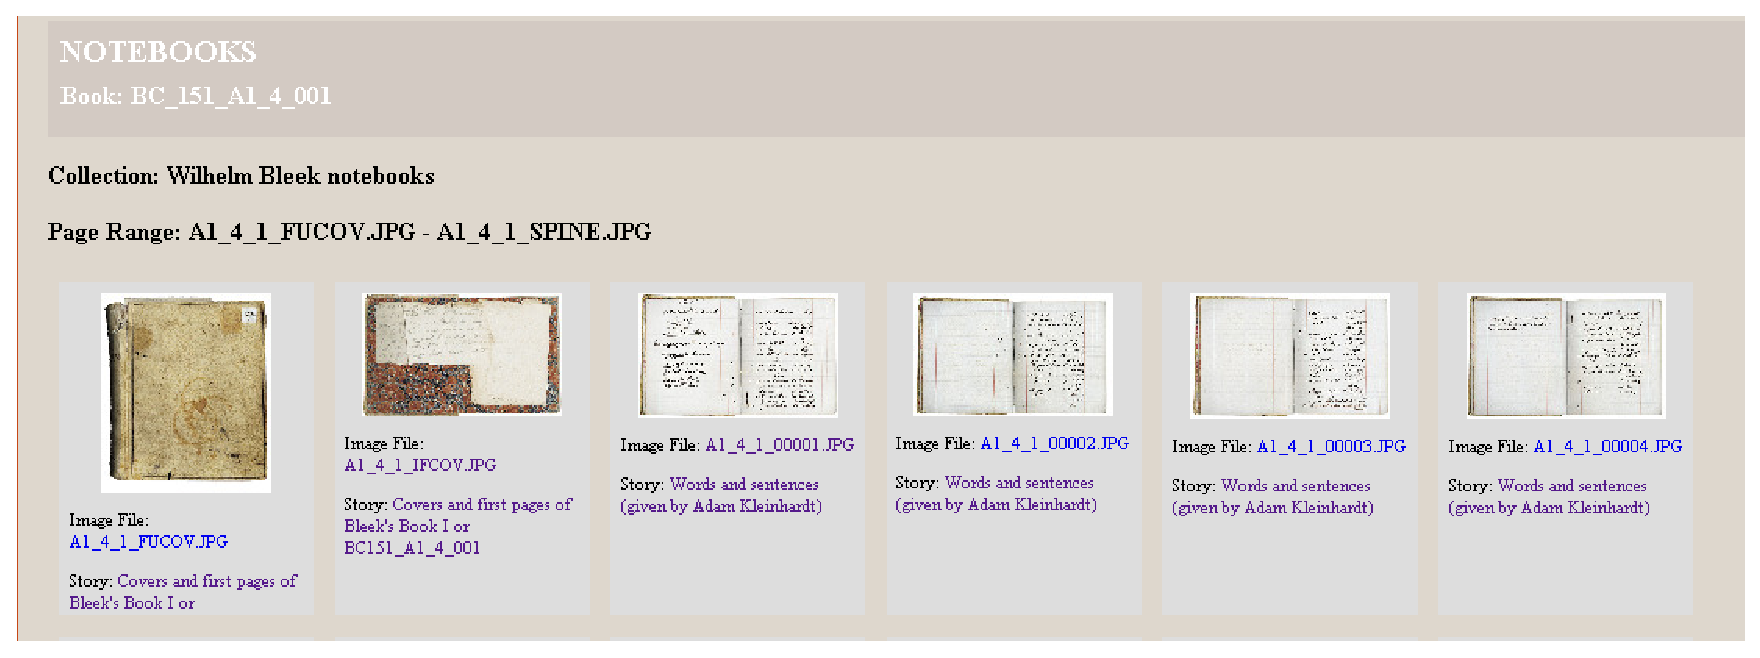
\includegraphics[width=0.95\textwidth]{%
 chapter03/figures/pilot-implementation-screenshot.eps}
 }%
 \caption{Pilot system user interface}
 \label{fig:pilot-study:pilot-system:user-interface}
\end{figure}

The user interface is rendered using statically-generated HTML files, that are
generated by applying XSLT stylesheets to individual metadata objects. The
metadata object structure is discussed in detail in Section
~\ref{sec:pilot-study:pilot-system:repository}

\subsection{Repository}
\label{sec:pilot-study:pilot-system:repository}

The repository sub-layer stores both the digital content and associated
representational information --metadata objects-- on the filesystem, alongside
each other, with the metadata objects stored in XML plain text files. The
digital objects are contained within hierarchical folders, hereon called
containers objects, that conform to the original original collection structure. 

The metadata file records were encoded using a qualified dublin application
profile \citep{Coyle2009} that was created specifically for the Bleek and Lloyd
collection, with each object having one associated metadata file. Three
distinct types of metadata objects were devised: container metadata objects,
illustrated in Listing ~\ref{lst:pilot-study:pilot-system:container}, are
essentially manifests of digital objects contained within them; virtual
objects, illustrated in Listing ~\ref{lst:pilot-study:pilot-system:virtual},
define the semantics of the images and collection as a whole by describing the
logical association of the images and collection; and digital content metadata
objects encode representational information specific to each individual image.

\lstinputlisting[float,frame=lines,caption=A digital content metadata file, label=lst:pilot-study:pilot-system:content, language=XML]{chapter03/code/digital-content.metadata}

\lstinputlisting[float,frame=lines, caption=A virtual object metadata file, label=lst:pilot-study:pilot-system:virtual,language=XML]{chapter03/code/virtual-object.metadata}

\lstinputlisting[float,frame=lines,caption=A container object metadata file,label=lst:pilot-study:pilot-system:container,language=XML]{ chapter03/code/container-object.metadata }
\section{Evaluation}
\label{sec:pilot-study:evaluation}

The main objective of the evaluation was to assess the impact of having
fragmented metadata files for each digital object, and in particular prove that
such a design approach would not negatively impact the static generation of the
collection.

The pilot system was thus evaluated by assessing its effectiveness, and the
digital Bleek and Lloyd collection \citep{Suleman2007} was used as
the case collection. The collection had previously been implemented by
generating static HTML files by parsing a single standalone XML file
containing metadata associated with the digital content \citep{Suleman2007}. An
overview of the Bleek and Lloyd collection is shown in Table
~\ref{tab:pilot-study:overview:collection-profile}.

%\subsection{Effectiveness}
%\label{sec:pilot-study:evaluation:effectiveness}
\tablespacing
%%%%%\begin{longtable}{p{0.4\linewidth} p{0.5\linewidth}}
\begin{longtable}{
>{\arraybackslash}p{0.30\linewidth}|
>{\arraybackslash}p{0.60\linewidth}}

\caption{Overview of the digital Bleek and Lloyd collection}
\label{tab:pilot-study:overview:collection-profile} \\

 %%%%%%\toprule
 %%%%%\textbf{} & \textbf{}\\
 \cline{1-2}
 \endfirsthead

 \caption[]{(continued)}\\
 %%%%%%\toprule
 %%%%%\textbf{} & \textbf{}\\
 \cline{1-2}
 \endhead

 % Page footer
 \midrule
 \multicolumn{2}{r}{(Continued on next page)} \\
 \endfoot

 % Last page footer
 %%%%%%\bottomrule
 \endlastfoot

 {\textbf{Collection theme}}&
 {Historical artifacts; museum objects}\\

 \cline{2-2}
 %\cmidrule[0.1pt](l{0.5em}r{0.5em}){1-2}

 {\textbf{Media types}}&
 {Digitised}\\

 \cline{2-2}
 %\cmidrule[0.1pt](l{0.5em}r{0.5em}){1-2}

 {\textbf{Collection size}}&
 {6.2GB}\\

 \cline{2-2}
 %\cmidrule[0.1pt](l{0.5em}r{0.5em}){1-2}

 {\textbf{Content type}}&
 {image/jpeg}\\

 \cline{2-2}
 %\cmidrule[0.1pt](l{0.5em}r{0.5em}){1-2}

 {\textbf{Number of collections}}&
 {\num{16}}\\

 \cline{2-2}
 %\cmidrule[0.1pt](l{0.5em}r{0.5em}){1-2}

 {\textbf{Number of objects}}&
 {\num{18924}}\\

 \end{longtable}

\bodyspacing

%\subsection{Discussion}
%\label{sec:pilot-study:evaluation:discussion}
\section{Conclusion}
\label{sec:pilot-study:summary}

The feasibility of conducting the proposed research was determined after
conducting the pilot study. In particular, the successful generation of the
Bleek and Lloyd collection provided the much needed evidence.

In addition, the pilot study helped uncover shortcomings in the general
approach used, effectively setting the course for the proposed research. Some
challenges that were identified include possible problems that would result
when handling large and complex collections, and the viability of statically
generating HTML files for collections with regularly changing content.
 % February 27, 2013 -- moved content to cases studies chapter
\chapter{Design principles\label{ch:exploratory-study}}

This chapter details the systematic process that was followed in order to
derive the guiding principles that can potentially simplify the design of
\gls{dl} services, effectively making then easier to work with.

The chapter is organised as follows: Section~\ref{sec:exploratory-study:research-perspective} outlines the rationale behind
conducting this exploratory study;
Section~\ref{sec:exploratory-study:research-perspective:research-questions}
introduces and describes the research method that was employed during this phase
of the research; Section~\ref{sec:exploratory-study:methodology} details the
process that was followed to collect and analyse the data; and finally, Section~\ref{sec:exploratory-study:summary} concludes the chapter.

\section{Research perspective}
\label{sec:exploratory-study:research-perspective}

\subsection{Prior research observations}
\label{sec:exploratory-study:research-perspective:prior-research-observations}

In our earlier work linked to this research, some issues that hinder
ubiquitous access to information and widespread preservation in Africa have
been highlighted \citep{Suleman2008}. A number of potential solutions to the
issues
raised have in the recent past also been presented, and take the form of
lightweight systems \citep{Suleman2007,Suleman2010a} with simplicity as
the key criterion.

However, the proposed solutions were solely based on specific user
requirements. The significance of prior work stems from the fact that they provided
this research with working hypotheses, which take the form of a set of
observable facts, that helped set the stage for the exploratory study.

\subsection{Research questions}
\label{sec:exploratory-study:research-perspective:research-questions}

The primary research question for this research, described in Section
\ref{sec:introduction:research-questions}, seeks to investigate the feasibility
of implementing \gls{dl} services that are based on simple
architectures. In order to better understand the simplicity of services, a
secondary research question, which was the main driving factor for the
exploratory study, was formulated as outlined below.

\begin{itemize}
 \item How should simplicity for \gls{dl} storage and service
architectures be defined?
\end{itemize}

The overall aim of the exploratory study was two-fold: firstly, it served to
guide the overall direction of the research, and secondly, it was aimed at
understanding contemporary \gls{dl} design in such a way as to be able to
better prescribe an alternative design approach that might result in simpler
\gls{dl} tools and services.

In order to obtain a reliable and comprehensive understanding of the desired
result, a qualitative study was conducted using a Grounded Theory approach.

\subsection{Summary}
\label{sec:exploratory-study:research-perspective:summary}

This section has highlighted prior work related to this research that
helped set the stage for the exploratory study. The section also outlined how
the exploratory study fits into the overall aims of the research by outlining
the rationale and significance of the study. In the subsequent section, the
research methods used during the exploratory study are discussed.
\section{Research methods}
\label{sec:exploratory-study:research-methods}

\subsection{Grounded theory}\index{Grounded theory}
\label{sec:exploratory-study:grounded-theory}

Grounded Theory is a research method that provides a technique for developing
theory iteratively from qualitative data. The goal of Grounded Theory is to
generate a theory that accounts for a pattern of behaviour that is relevant for those involved \citep{Glaser1978}. Grounded Theory attempts to find the main concern of the participants and how they go about resolving it, through constant comparison of data at increasing levels of abstraction and has also been described as ``a general pattern for understanding'' \citep{Glaser1992}.

The Grounded Theory method generally revolves around a series of five
steps, as outlined below.

\subsubsection{Grounded theory process}

\paragraph{Step 1} Data collection

This step uses a method appropriate to the research context to elicit
information from selected participants. Typical methods include
conducting semi-structured interviews.

\paragraph{Step 2} Data analysis

The data analysis step forms the core of grounded theory and generally involves
the use of a constant comparative method to generate and analyse data.

\paragraph{Step 3} Memoing\index{Memoing}

Memoing, as the name suggests, involves writing theoretical memos to identify
relationships between different patterns of the data.

\paragraph{Step 4} Sorting

The sorting step takes the form of arranging all memos once the data collection
becomes saturated. The outcome of this results in a theory describing how the
identified categories relate to the core category.

\paragraph{Step 5} Theoretical coding

The data collected is divided into segments to identify categories or themes.
The categorised data is then further examined to identify properties common to
each of the categories.

Grounded theory was selected as the primary research method for the exploratory
study due to the following reasons:

\begin{itemize}
 \item It is primarily aimed at theory generation, focusing specifically on
generating theoretical ideas, explanations and understanding of the data.
 \item It is useful when trying to gain a fresh perspective of a
well-known area.
  \item It has proven to be a successful method for exploring human and social
aspects.
  \item It is by far one of the most common/popular analytic technique in
qualitative analysis.
  \item It is arguably intuitive.
\end{itemize}


\subsection{Analytic hierarchy process}\index{Analytic hierarchy process}
\label{sec:exploratory-study:ahp}

The \gls{ahp} is a theory of measurement through
pairwise comparisons that relies on judgement of experts to derive priority scales
\citep{Saaty2008}. A pairwise comparison is a problem-solving technique that
allows one to determine the the most significant item among a group of items. The overall
process is driven by scales of absolute judgement that represent how much more
an element dominates another with respect to a given attribute. The pairwise
comparison method involves following a series of steps and is outlined in
Section~\ref{sec:exploratory-study:research-methods:ahp:pairwise}.

\subsubsection{Pairwise comparisons method}\index{Pairwise comparisons}
\label{sec:exploratory-study:research-methods:ahp:pairwise}

The method of pairwise comparisons ensures that for a given set of elements or
alternatives, each candidate element is matched head to head with the other
candidates and is performed by decomposing decisions \citep{Saaty2008} into the
steps outlined below.

\paragraph{Step 1} Define the criteria to be ranked. 

The criteria identified are influenced by the overall objectives and form the
basis of the comparative analysis.

\paragraph{Step 2} Arrange the criteria in an $N\times N$ matrix.

In essence, each element in a given set a of $N$ elements is compared against
other alternatives in the set as shown in Table~\ref{tab:exploratory-study:ahp:matrix}. The total number of pairwise
comparisons can thus be computed using equation:

\begin{equation*}
%\label{eq:exploratory-study:research-methods:pairwise}
 \frac{N (N-1)}{2}
\end{equation*}

\tablespacing
%%%%%\begin{longtable}{p{0.05\linewidth} p{0.05\linewidth} p{0.05\linewidth}
%%%%%p{0.05\linewidth} p{0.05\linewidth} p{0.05\linewidth} p{0.05\linewidth}
%%%%%p{0.05\linewidth} p{0.05\linewidth} p{0.05\linewidth} p{0.05\linewidth}}
\begin{longtable}{
>{\centering\arraybackslash}m{0.05\linewidth}
|>{\centering\arraybackslash}m{0.05\linewidth}
|>{\centering\arraybackslash}m{0.05\linewidth}
|>{\centering\arraybackslash}m{0.05\linewidth}
|>{\centering\arraybackslash}m{0.05\linewidth}
|>{\centering\arraybackslash}m{0.05\linewidth}
|>{\centering\arraybackslash}m{0.05\linewidth}
|>{\centering\arraybackslash}m{0.05\linewidth}
|>{\centering\arraybackslash}m{0.05\linewidth}
|>{\centering\arraybackslash}m{0.05\linewidth}|
>{\centering\arraybackslash}m{0.05\linewidth}}

\caption{An $N\times N$ pairwise comparisons matrix}
\label{tab:exploratory-study:ahp:matrix} \\

 %%%%%\toprule
 \cline{3-10}
 \multicolumn{1}{c}{} &
 \multicolumn{1}{c|}{} &
 \textbf{H} &
 \textbf{G} &
 \textbf{F} &
 \textbf{E} &
 \textbf{D} &
 \textbf{C} &
 \textbf{B} &
 \textbf{A} &
 {} \\
 \cline{2-10}
 %%%%%\midrule
 \cline{2-10}
 \endfirsthead

 \caption[]{(continued)}\\
 %%%%%\toprule
 \cline{3-10}
 \multicolumn{1}{c}{} &
 \multicolumn{1}{c|}{} &
 \textbf{H} &
 \textbf{G} &
 \textbf{F} &
 \textbf{E} &
 \textbf{D} &
 \textbf{C} &
 \textbf{B} &
 \textbf{A} &
 {} \\
 %%%%%\midrule
 \cline{2-10}
 \endhead

 % Page footer
 %%%%%\midrule
 \cline{2-10}
 \multicolumn{9}{r}{(Continued on next page)} \\
 \endfoot

 % Last page footer
 %%%%%\bottomrule
 \endlastfoot

 \multicolumn{1}{c|}{}&
 \textbf{A}&
 {X}&
 {X}&
 {X}&
 {X}&
 {X}&
 {X}&
 {X}&
 \multicolumn{1}{c}{}&
 \multicolumn{1}{c}{}\\

 \cline{2-9}
 %\cmidrule[0.1pt](l{0.5em}r{0.5em}){1-7}

 \multicolumn{1}{c|}{}&
 \textbf{B}&
 {X}&
 {X}&
 {X}&
 {X}&
 {X}&
 {X}&
 \multicolumn{1}{c}{}&
 \multicolumn{1}{c}{}&
 \multicolumn{1}{c}{}\\

 \cline{2-8}
 %\cmidrule[0.1pt](l{0.5em}r{0.5em}){1-7}

 \multicolumn{1}{c|}{}&
 \textbf{C}&
 {X}&
 {X}&
 {X}&
 {X}&
 {X}&
 \multicolumn{1}{c}{}&
 \multicolumn{1}{c}{}&
 \multicolumn{1}{c}{}&
 \multicolumn{1}{c}{}\\

 \cline{2-7}
 %\cmidrule[0.1pt](l{0.5em}r{0.5em}){1-7}

 \multicolumn{1}{c|}{}&
 \textbf{D}&
 {X}&
 {X}&
 {X}&
 {X}&
 \multicolumn{1}{c}{}&
 \multicolumn{1}{c}{}&
 \multicolumn{1}{c}{}&
 \multicolumn{1}{c}{}&
 \multicolumn{1}{c}{}\\

 \cline{2-6}
 %\cmidrule[0.1pt](l{0.5em}r{0.5em}){1-7}

 \multicolumn{1}{c|}{}&
 \textbf{E}&
 {X}&
 {X}&
 {X}&
 \multicolumn{1}{c}{}&
 \multicolumn{1}{c}{}&
 \multicolumn{1}{c}{}&
 \multicolumn{1}{c}{}&
 \multicolumn{1}{c}{}&
 \multicolumn{1}{c}{}\\

 \cline{2-5}
 %\cmidrule[0.1pt](l{0.5em}r{0.5em}){1-7}
 
 \multicolumn{1}{c|}{}&
 \textbf{F}&
 {X}&
 {X}&
 \multicolumn{1}{c}{}&
 \multicolumn{1}{c}{}&
 \multicolumn{1}{c}{}&
 \multicolumn{1}{c}{}&
 \multicolumn{1}{c}{}&
 \multicolumn{1}{c}{}&
 \multicolumn{1}{c}{}\\
 
 \cline{2-4}

 \multicolumn{1}{c|}{}&
 \textbf{G}&
 {X}&
 \multicolumn{1}{c}{}&
 \multicolumn{1}{c}{}&
 \multicolumn{1}{c}{}&
 \multicolumn{1}{c}{}&
 \multicolumn{1}{c}{}&
 \multicolumn{1}{c}{}&
 \multicolumn{1}{c}{}&
 \multicolumn{1}{c}{}\\
 
 \cline{2-3}

 \multicolumn{1}{c|}{}&
 \textbf{H}&
 \multicolumn{1}{c}{}&
 \multicolumn{1}{c}{}&
 \multicolumn{1}{c}{}&
 \multicolumn{1}{c}{}&
 \multicolumn{1}{c}{}&
 \multicolumn{1}{c}{}&
 \multicolumn{1}{c}{}&
 \multicolumn{1}{c}{}&
 \multicolumn{1}{c}{}\\

\cline{2-2}
 
\end{longtable}

\bodyspacing

\paragraph{Step 3} Compare pairs of items. 

Each criterion is compared again
other alternatives to determine the relative important of the characteristic.

\paragraph{Step 4} Create the ranking of items. 

A ranking system is created
based on the relative occurrence of each element in the matrix.

The use of pairwise comparisons was particularly useful in the research context
as the method is ideal for ranking a set of decision-making criteria and rate
the criteria on a relative scale of importance.

\subsection{Summary}
\label{sec:exploratory-study:research-methods:summary}

This section has described the two primary research methods that were used
during the exploratory phase of this research. The combined effect of using the
two methods is appropriate as the exploratory study involved a series of
qualitative phases. The details of the study are outlined in Section~\ref{sec:exploratory-study:methodology}.
\section{General approach}
\label{sec:exploratory-study:methodology}

\subsection{Data collection}
\label{sec:exploratory-study:methodology:case-software-tools}

A meta-analysis\index{Meta-analysis} involving a total of 12 software applications
was systematically conducted to facilitate the compilation of a comprehensive
and inclusive set of principles. The set of tools comprised six
\gls{dl} software applications and six non-\gls{dl}
software applications. The selection of the six \gls{dl} software
was done on the basis of popularity as depicted on
OpenDOAR\footnote{\url{http://www.opendoar.org}}\index{OpenDOAR}. Table~\ref{tab:exploratory-study:methodology:case-software} outlines the 12 candidate tools that were considered.

The relevant software attributes that may have influenced the design decisions
of the applications were then identified. The pairwise comparisons method,
outlined in Section~\ref{sec:exploratory-study:research-methods:ahp:pairwise} was then used as
the constant comparison method during the data analysis stage. The data
analysis stage is discussed in more detail in Section~\ref{sec:exploratory-study:methodology:data-analysis}

% Software applications table

\tablespacing
%%%%%\begin{longtable}{p{0.25\linewidth} p{0.25\linewidth} p{0.4\linewidth}}
\begin{longtable}{
>{\arraybackslash}p{0.22\linewidth}|
>{\arraybackslash}p{0.20\linewidth}|
>{\arraybackslash}p{0.48\linewidth}}

\caption{Software applications used for pairwise comparisons}
\label{tab:exploratory-study:methodology:case-software} \\

 %%%%%\toprule
 %%%%%\hline
 \textbf{Application} & \textbf{Category} & \textbf{Description}\\
 %%%%%\midrule
 \cline{1-3}
 \endfirsthead

 \caption[]{(continued)}\\
 %%%%%\toprule
 %%%%%\hline
 \textbf{Application} & \textbf{Category} & \textbf{Description}\\
 %%%%%\midrule
 \cline{1-3}
 \endhead

 % Page footer
 %%%%%\midrule
 %%%%%\hline
 \multicolumn{3}{r}{(Continued on next page)} \\
 \endfoot

 % Last page footer
 %%%%%\bottomrule
 \endlastfoot

 \textbf{DSpace\footnote{\url{http://www.dspace.org}}}&
 {DL software}&
 {A general digital asset management software}\\

 \cline{1-3}
 %\cmidrule[0.1pt](l{0.5em}r{0.5em}){1-3}

 \textbf{EPrints\footnote{\url{http://www.eprints.org}}}&
 {DL software}&
 {A general digital repository software package}\\

 \cline{1-3}
 %\cmidrule[0.1pt](l{0.5em}r{0.5em}){1-3}

 \textbf{ETD-db\footnote{\url{http://scholar.lib.vt.edu/ETD-db}}}&
 {DL software}&
 {An electronic thesis and dissertation software package}\\

 \cline{1-3}
 %\cmidrule[0.1pt](l{0.5em}r{0.5em}){1-3}

 \textbf{FedoraCommons\footnote{\url{http://fedora-commons.org}}}&
 {DL software}&
 {A general digital object repository framework}\\

 \cline{1-3}
 %\cmidrule[0.1pt](l{0.5em}r{0.5em}){1-3}

 \textbf{Greenstone\footnote{\url{http://www.greenstone.org}}}&
 {DL software}&
 {A general digital collection management software}\\

 \cline{1-3}
 %\cmidrule[0.1pt](l{0.5em}r{0.5em}){1-3}

 \textbf{CDS Invenio\footnote{\url{http://invenio-software.org}}}&
 {DL Software}&
 {A general document repository software package}\\

 \cline{1-3}
 %%%%%\cmidrule[0.1pt](l{0.5em}r{0.5em}){1-3}
 %%%%%\cline{1-3}

 \textbf{Facebook\footnote{\url{http://www.facebook.com}}}&
 {Non DL software}&
 {A free social network portal/Website}\\

 \cline{1-3}
 %\cmidrule[0.1pt](l{0.5em}r{0.5em}){1-3}

 \textbf{Gmail\footnote{\url{https://mail.google.com}}}&
 {Non DL software}&
 {A free email messaging hosted-service platform}\\

 \cline{1-3}
 %\cmidrule[0.1pt](l{0.5em}r{0.5em}){1-3}

 \textbf{MixIt\footnote{\url{http://www.mixit.com}}}&
 {Non DL software}&
 {A free instant messaging Web application}\\

 \cline{1-3}
 %\cmidrule[0.1pt](l{0.5em}r{0.5em}){1-3}

 \textbf{Moodle\footnote{\url{http://moodle.org}}}&
 {Non DL software}&
 {A free e-learning management platform}\\

 \cline{1-3}
 %\cmidrule[0.1pt](l{0.5em}r{0.5em}){1-3}

 \textbf{Ushahidi\footnote{\url{http://www.ushahidi.com}}}&
 {Non DL software}&
 {An information collection and visualisation platform}\\

 \cline{1-3}
 %\cmidrule[0.1pt](l{0.5em}r{0.5em}){1-3}

 \textbf{WordPress\footnote{\url{http://wordpress.org}}}&
 {Non DL software}&
 {A standalone blogging software package}\\

 \end{longtable}

\bodyspacing

\subsection{Data analysis}
\label{sec:exploratory-study:methodology:data-analysis}

The set of all possible software attributes that can potentially influence
design decisions of software applications were identified and arranged based on
whether they were specific to the two sets of software applications---Digital
Library software and non-\gls{dl} software---or both sets. Table~\ref{tab:exploratory-study:methodology:software-attributes} shows the
software attributes, that were considered,  as pertains to whether they affect
\gls{dl} software, non-\gls{dl} software, or both.

\tablespacing
%%%%%\begin{longtable}{p{0.45\linewidth} p{0.15\linewidth} p{0.15\linewidth}
%%%%%p{0.15\linewidth}}
\begin{longtable}{
>{\arraybackslash}p{0.35\linewidth}|
>{\centering\arraybackslash}p{0.15\linewidth}|
>{\centering\arraybackslash}p{0.15\linewidth}|
>{\centering\arraybackslash}p{0.15\linewidth}}

\caption{Software attributes considered in pairwise comparisons}
\label{tab:exploratory-study:methodology:software-attributes} \\

 %%%%%\toprule
 %%%%%\hline
 %%%%%\textbf{} & 
 %%%%%\multicolumn{3}{c}{\textbf{Software Category}}\\
 %%%%%\midrule
 %%%%%\cline{2-4}
 \textbf{} &
 \textbf{DL} &
 \textbf{Non-DL} &
 \textbf{Both} \\
 %%%%%\midrule
 \cline{1-4}
 \endfirsthead

 \caption[]{(continued)}\\
 %%%%%\toprule
 %%%%%\hline
 %%%%%\textbf{} & 
 %%%%%\multicolumn{3}{c}{\textbf{Software Category}}\\
 %%%%%\midrule
 %%%%%\cline{2-4}
 \textbf{} &
 \textbf{DL} &
 \textbf{Non-DL} &
 \textbf{Both} \\
 %%%%%\midrule
 \cline{1-4}
 \endhead

 % Page footer
 %%%%%\midrule
 %%%%%\hline
 \multicolumn{4}{r}{(Continued on next page)} \\
 \endfoot

 % Last page footer
 %%%%%\bottomrule
 \endlastfoot

 \textbf{Digital content}&
 {X}&
 {}&
 {}\\

 \cline{1-4}
 %\cmidrule[0.1pt](l{0.5em}r{0.5em}){1-3}

 \textbf{Media types}&
 {X}&
 {}&
 {}\\

 \cline{1-4}
 %\cmidrule[0.1pt](l{0.5em}r{0.5em}){1-3}

 \textbf{Metadata objects}&
 {X}&
 {}&
 {}\\

 \cline{1-4}
 %\cmidrule[0.1pt](l{0.5em}r{0.5em}){1-3}

 \textbf{Data access}&
 {}&
 {}&
 {X}\\

 \cline{1-4}
 %\cmidrule[0.1pt](l{0.5em}r{0.5em}){1-3}

 \textbf{Information structure}&
 {X}&
 {}&
 {}\\

 \cline{1-4}
 %\cmidrule[0.1pt](l{0.5em}r{0.5em}){1-3}

 \textbf{Core language}&
 {}&
 {}&
 {X}\\

 \cline{1-4}
 %\cmidrule[0.1pt](l{0.5em}r{0.5em}){1-3}

 \textbf{Content delivery}&
 {}&
 {}&
 {X}\\

 \cline{1-4}
 %\cmidrule[0.1pt](l{0.5em}r{0.5em}){1-3}

 \textbf{Deployment platform}&
 {}&
 {}&
 {X}\\

 \cline{1-4}
 %\cmidrule[0.1pt](l{0.5em}r{0.5em}){1-3}

 \textbf{Software dependencies}&
 {}&
 {}&
 {X}\\

 \cline{1-4}
 %\cmidrule[0.1pt](l{0.5em}r{0.5em}){1-3}

 \textbf{Flexibility}&
 {}&
 {}&
 {X}\\

 \cline{1-4}
 %\cmidrule[0.1pt](l{0.5em}r{0.5em}){1-3}

 \textbf{Preservation strategy}&
 {X}&
 {}&
 {}\\

 \cline{1-4}
 %\cmidrule[0.1pt](l{0.5em}r{0.5em}){1-3}

 \textbf{Extensibility}&
 {}&
 {}&
 {X}\\

 \cline{1-4}
 %\cmidrule[0.1pt](l{0.5em}r{0.5em}){1-3}

 \textbf{Standardisation}&
 {}&
 {}&
 {X}\\

 \cline{1-4}
 %\cmidrule[0.1pt](l{0.5em}r{0.5em}){1-3}

 \textbf{Interoperability}&
 {}&
 {}&
 {X}\\

 \cline{1-4}
 %\cmidrule[0.1pt](l{0.5em}r{0.5em}){1-3}

 \textbf{Ease of installation}&
 {}&
 {}&
 {X}\\

 \cline{1-4}
 %\cmidrule[0.1pt](l{0.5em}r{0.5em}){1-3}

 \textbf{Objects accessibility}&
 {X}&
 {}&
 {}\\

 \cline{1-4}
 %\cmidrule[0.1pt](l{0.5em}r{0.5em}){1-3}

 \textbf{Objects naming scheme}&
 {X}&
 {}&
 {}\\

 \cline{1-4}
 %\cmidrule[0.1pt](l{0.5em}r{0.5em}){1-3}

 \textbf{Hosting}&
 {}&
 {}&
 {X}\\

 \cline{1-4}
 %\cmidrule[0.1pt](l{0.5em}r{0.5em}){1-3}
 
 \textbf{Scalability}&
 {}&
 {}&
 {X}\\

 \cline{1-4}
 %\cmidrule[0.1pt](l{0.5em}r{0.5em}){1-3}
 
 \textbf{Reliability}&
 {}&
 {}&
 {X}\\

 \cline{1-4}
 %\cmidrule[0.1pt](l{0.5em}r{0.5em}){1-3}
 
 \textbf{Usability}&
 {}&
 {}&
 {X}\\

 \cline{1-4}
 %\cmidrule[0.1pt](l{0.5em}r{0.5em}){1-3}

 \textbf{Mobile friendly}&
 {}&
 {}&
 {X}\\

 %%%%%\cline{1-4}
 %\cmidrule[0.1pt](l{0.5em}r{0.5em}){1-3}

 \end{longtable}

\bodyspacing

Open coding\index{Open Coding} \citep{Glaser1992} was used during the data analysis
process, and a head-to-head pairwise comparison was then performed on each of
the 12 applications against the other alternatives using the
pairwise comparisons method procedure described in Section~\ref{sec:exploratory-study:research-methods:ahp:pairwise}. All in all, a total
of 66 pairwise comparisons, derived using the equation in Section~\ref{sec:exploratory-study:research-methods:ahp:pairwise}, were conducted. 
%A template showing the detailed comparative attributes is shown in Table~\ref{tab:exploratory-study:methodology:digital-library-software} in Appendix~\ref{ch:appendex-a:exploratory-study}

The Memoing process\index{Memoing}, for each of the 66 comparisons, involved
identifying design choice for each software attribute and the possible
corresponding design rationale\index{Design Rationale}. All possible potential design decisions that
could be applicable to the design of simple and minimalistic architectures were
subsequently identified. Figure~\ref{fig:exploratory-study:general-approach:data-analysis:memoing-process}
shows an excerpt of the memoing process.

\begin{figure}
 \begin{center}
 \fbox{
 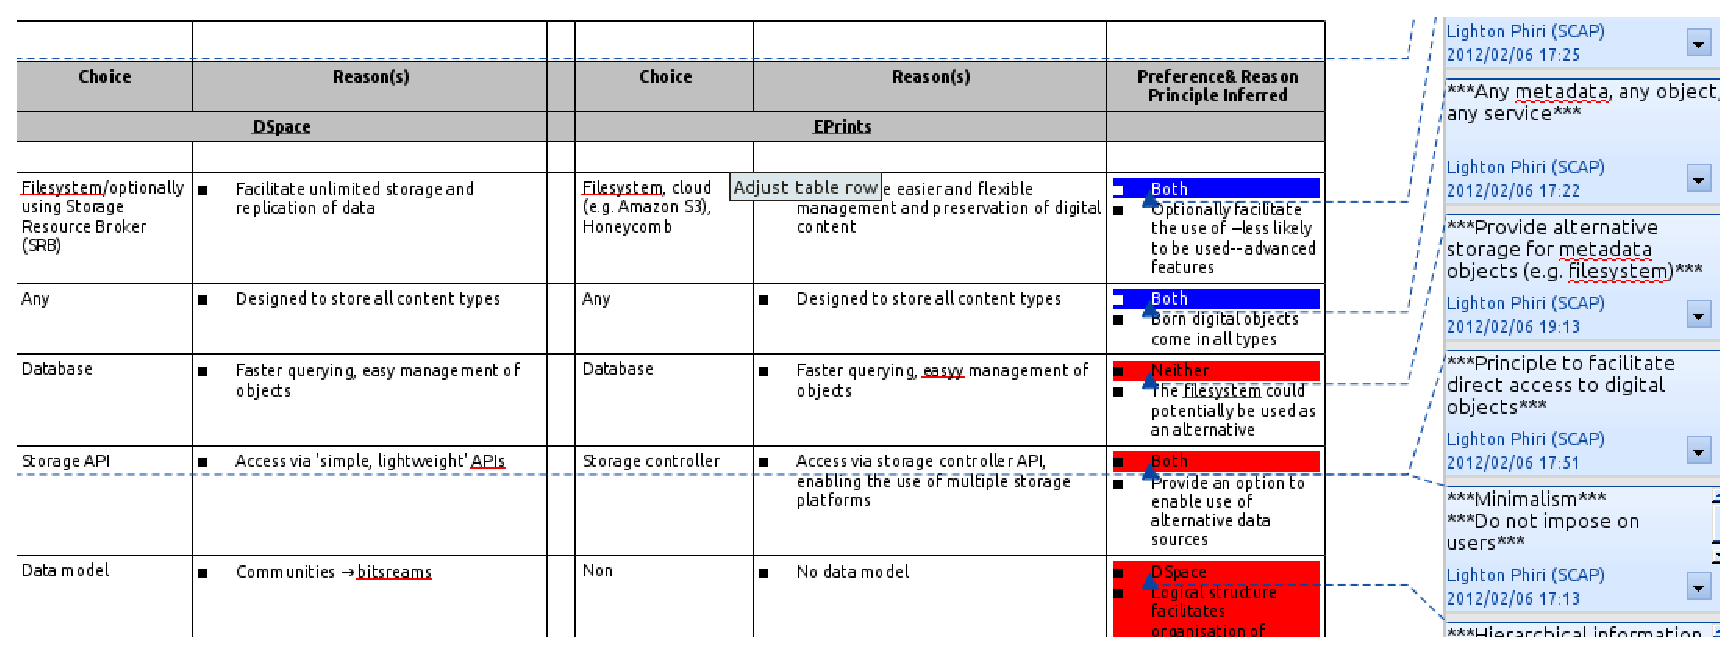
\includegraphics[width=0.95\textwidth]{%
chapter04/figures/grounded-theory-memoing.eps}
 }
 \caption[Screenshot showing an excerpt of the GT memoing process]{Screenshot showing an excerpt of the grounded theory memoing process}
 \label{fig:exploratory-study:general-approach:data-analysis:memoing-process}
 \end{center}
\end{figure}



% Defunct now---September 19, 2012
%
%Table showing attributes considered during general pairwise comparisons for all
%tools

%\tablespacing
%\begin{landscape}
%\begin{longtable}{p{0.25\linewidth} p{0.13\linewidth} p{0.13\linewidth}
p{0.13\linewidth} p{0.13\linewidth} p{0.13\linewidth}}

\caption{General Software Feature Pairwise Comparisons Matrix}
\label{tab:exploratory-study:methodology:general-software} \\

 \toprule
{} & \multicolumn{2}{c}{\textbf{Application 1}} &
\multicolumn{2}{c}{\textbf{Application 2}} & {}\\
 \midrule
\textbf{Attribute} & \textbf{Choice} & \textbf{Reason} & \textbf{Choice} &
\textbf{Reason} & \textbf{Comments}\\
 \midrule
 \endfirsthead

 \caption[]{(continued)}\\
 \toprule
{} & \multicolumn{2}{c}{\textbf{Application 1}} &
\multicolumn{2}{c}{\textbf{Application 2}} & {}\\
 \midrule
\textbf{Attribute} & \textbf{Choice} & \textbf{Reason} & \textbf{Choice} &
\textbf{Reason} & \textbf{Comments}\\
 \midrule
 \endhead

 % Page footer
 \midrule
 \multicolumn{6}{r}{(Continued on next page)} \\
 \endfoot

 % Last page footer
 \bottomrule
 \endlastfoot

 %\cmidrule[0.1pt](l{0.5em}r{0.5em}){1-6}

 {Hosting}&
 {\ldots}&
 {\ldots}&
 {\ldots}&
 {\ldots}&
 {\ldots}\\

 \cmidrule[0.1pt](l{0.5em}r{0.5em}){1-6}

 {Extensibility}&
 {\ldots}&
 {\ldots}&
 {\ldots}&
 {\ldots}&
 {\ldots}\\

 \cmidrule[0.1pt](l{0.5em}r{0.5em}){1-6}

 {Scalability}&
 {\ldots}&
 {\ldots}&
 {\ldots}&
 {\ldots}&
 {\ldots}\\

 \cmidrule[0.1pt](l{0.5em}r{0.5em}){1-6}

 {Reliability}&
 {\ldots}&
 {\ldots}&
 {\ldots}&
 {\ldots}&
 {\ldots}\\

 \cmidrule[0.1pt](l{0.5em}r{0.5em}){1-6}

 {Usability}&
 {\ldots}&
 {\ldots}&
 {\ldots}&
 {\ldots}&
 {\ldots}\\

 \cmidrule[0.1pt](l{0.5em}r{0.5em}){1-6}

 {Mobile Friendly}&
 {\ldots}&
 {\ldots}&
 {\ldots}&
 {\ldots}&
 {\ldots}\\

 \cmidrule[0.1pt](l{0.5em}r{0.5em}){1-6}

 {Interoperability}&
 {\ldots}&
 {\ldots}&
 {\ldots}&
 {\ldots}&
 {\ldots}\\

 \end{longtable}

%\end{landscape}
%\bodyspacing

\subsection{Design principles}
\label{sec:exploratory-study:methodology:design-principles}

The major outcome of the exploratory study is a set of eight
guiding design principles for simple and minimalistic architectures of digital
libraries tools and/or services. It is premised that \gls{dl} software
designed and implemented based on these guiding principles could ultimately
be easy to use and maintain in the long run. The design principles are as
follows:

\begin{comment}
 design principles illustration
 https://www-01.ibm.com/software/ucd/designconcepts/designbasics.html
\end{comment}


\paragraph{Principle 1.} Hardware and/or software platform independence

\subparagraph{Description} It should be possible to operate tools and services
on
a wide variety of hardware and software platforms. The rationale behind this
principle is to ensure that the least possible cost associated to technological
infrastructure is incurred during the collection management life-cycle.

%\paragraph{Rationale} xxx

\subparagraph{Discussion} The preservation\index{Preservation} life-cycle of digital objects is an
on-going process that typically involves the management of digital content and
its associated representational information. The cost implications of long-term
digital preservation\index{Preservation} is a crucial task for both small and large-scale
preservation projects \citep{View2002}. However, the vast majority of
organisations involved in the curation and preservation\index{Preservation} of digital information
usually do not have adequate funding to support this process. In addition, a
number of such organisations, in particular heritage organisations, do not have
sustainable funding models to ensure the on-going process of managing digital
objects.

A reduction in the cost associated to the collection management process could be
archived in various ways including, but not limited to the following:

\begin{itemize}
 \item Designing tools that require minimal technical expertise to manage
 \item Designing tools capable of being run on popular of operating systems
 \item Designing tools capable of being operated on hardware platforms with
minimal specifications
\end{itemize}


\paragraph{Principle 2.} Heterogeneous object, metadata and service integration

\subparagraph{Description} There should be explicit support for integration of
any
digital object type, metadata format or new service.

%\paragraph{Rationale} xxx

\subparagraph{Discussion} The proliferation of both born-digital and digitised
information has given rise to various data formats and a corresponding increase
in the number of metadata standards, as discussed in Section~\ref{sec:background:fundamental-concepts:metadata}. In addition, there is a
growing demand for \gls{dl} services in order to facilitate ubiquitous
access to information.

Due to the aforementioned, it is imperative that the designed of digital
library tools be flexible enough to accommodate heterogeneous
objects, metadata and services. In a nutshell, the design should be based on a
``one size fits all'' approach.

\paragraph{Principle 3.} Support for community and international standards

\subparagraph{Description} The design of tools and services should take into
account community-based standards and international standards in order to
facilitate interoperability.

%\paragraph{Rationale}

\subparagraph{Discussion} The increase in the amount of digital content
generated and made available publicly has brought about a need to
standardise processes in the digital curation workflow. Section~\ref{sec:background:fundamental-concepts:standards} outlines the important
role that standards play and also discusses some of the popular \gls{dl}
standards.

Incorporating standards in the initial stages of the design process would
effectively ensure that the resulting \gls{dl} services becomes
interoperable with other external services. It also makes it easier for service
to be customised.

\paragraph{Principle 4.} Flexible design to facilitate extensibility

\subparagraph{Description} The design should be flexible enough to enable end
users to adapt the tools and services to their own needs.

%\paragraph{Rationale} xxx

\subparagraph{Discussion} Digital curation is slowly becoming a ubiquitous
process, and \glspl{dl} are increasingly being used in a wide array of
application domains---example application domains are highlighted in Section~\ref{sec:background:digital-libraries:application-domains}. 

The services offered by these different application domains varying and it is
imperative that the overall design be flexible enough to facilitate
customisation and extensibility.

\paragraph{Principle 5.} Minimalist design approach

\subparagraph{Description} There should be minimal use of external software
components in order to simplify the overall design. This would arguably result
in tools that are easier to manage.

%\paragraph{Rationale} xxx

\subparagraph{Discussion} The design of services should, at a minimum, only be
composed of the least number of components that are required for it to
function. Auxiliary external components should be made optional, making them
available only when required.

In addition, mandatory components should be critically analysed to ensure that
they make use of simplest possible solutions and/or technologies.

\paragraph{Principle 6.} Simplified preservation\index{Preservation} process

\subparagraph{Description} The preservation\index{Preservation} process should be simplified as much
as possible to make it possible to easily migrate digital content.

%\paragraph{Rationale} xxx

\subparagraph{Discussion} The preservation\index{Preservation} lifecylce is an on-going process
that requires dedicated staff. The majority of contemporary \gls{dl}
services require technology experts to perform the routine preservation\index{Preservation} tasks.

The overall design should thus be made as simple as possible so that novice
users are able to perform the most basic of preservation\index{Preservation} tasks.

\paragraph{Principle 7.} Structured Organisation of Data

\subparagraph{Description} There should be explicit support for hierarchical
logical organisation of information.

%\paragraph{Rationale} xxx

\subparagraph{Discussion} The majority of data that is curated and made
accessible publicly necessitates the logical organisation of information to
facilitate relationships that might exist between different data views. In
addition, data consumers usually visualise information using varying logical
views.

The design should thus explicitly support the logical organisation of
information, and optionally make it flexible enough for users to define the
desired logical views and structures.

\paragraph{Principle 8.} Design for least possible resources

\subparagraph{Description} There should be support for access to digital
collections in environments with resource constraints.

%\paragraph{Rationale} xxx

\subparagraph{Discussion} One of the motivating factors, outlined in Section~\ref{sec:introduction:motivation}, behind this research was the
unavailability of \gls{dl} tools that can effectively operate in
resource constrained environments. This is still a growing need for most
environments in developing countries, such as those found in Africa.

The design of \gls{dl} services should thus be based on the least
possible resources to enable resulting service operate in environments with
limited resources.

\subsection{Summary}
\label{sec:exploratory-study:methodology:summary}

This section discussed the procedure that was followed to derived a set of
design guiding principles that, when employed during the design of digital
library services, may potentially result in simpler services. Grounded Theory
was used as the overarching method during the derivation process and Table~\ref{tab:exploratory-study:methodology:grounded-theory-approach} shows a
summary of how the Grounded Theory steps were undertaken.

\tablespacing
%%%%%\begin{longtable}{p{0.3\linewidth} p{0.6\linewidth}}
\begin{longtable}{
>{\arraybackslash}p{0.24\linewidth}|
>{\arraybackslash}p{0.66\linewidth}}

\caption{Grounded theory general approach}
\label{tab:exploratory-study:methodology:grounded-theory-approach} \\

 %%%%%\toprule
 %%%%%\hline
 \textbf{Stage} & \textbf{Description}\\
 %%%%%\midrule
 %%%%%\hline
 \cline{1-2}
 \endfirsthead

 \caption[]{(continued)}\\
 %%%%%\toprule
 %%%%%\hline
 \textbf{Stage} & \textbf{Description}\\
 %%%%%\midrule
 %%%%%\hline
 \endhead

 % Page footer
 %%%%%\midrule
 %%%%%\hline
 \multicolumn{2}{r}{(Continued on next page)} \\
 \endfoot

 % Last page footer
 %%%%%\bottomrule
 \endlastfoot

 {\textbf{Data Collection}}&
 {A meta-analysis review of 12 software applications was conducted}\\

 %%%%%\cmidrule[0.1pt](l{0.5em}r{0.5em}){1-2}
 \cline{1-2}

 {\textbf{Data Analysis}}&
 {Pairwise comparisons were used at the constant comparative method}\\

 %%%%%\cmidrule[0.1pt](l{0.5em}r{0.5em}){1-2}
 \cline{1-2}

 {\textbf{Memoing}} &
 {Memos were created using a general note taking process}\\

 %%%%%\cmidrule[0.1pt](l{0.5em}r{0.5em}){1-2}
 \cline{1-2}

 {\textbf{Sorting}} &
 {Arranged conceptual levels based on meta-level of attribute being investigated} \\

 %%%%%\cmidrule[0.1pt](l{0.5em}r{0.5em}){1-2}
 \cline{1-2}

 {\textbf{Coding}} &
 {The coding process took place in tandem with the data collection process and open coding was used}\\

 %%%%%\cmidrule[0.1pt](l{0.5em}r{0.5em}){1-2}
 %%%%%\cline{1-2}

 \end{longtable}

\bodyspacing
\section{Summary}
\label{sec:exploratory-study:summary}

This chapter discussed the derivation process of a set of design principles
applicable for the design of simple \gls{dl} services which can easily
be operated in resource constrained environments. The development of
applications for resource constrained environments requires careful
consideration and eliciting these requirements during the early stages of the
design process may ensure that the resulting services become tailored for such
domains.

In summary, all the design principles were derived with simplicity and
minimalism and the key criterion.

\chapter{Designing for simplicity\label{ch:implementation}}

In Chapter~\ref{ch:exploratory-study}, a set of design principles, and the systematic approach used to derived them was outlined. The derived design principles can be applied during the design of the different components of a \gls{dls}---user interface, repository and service layer.

In this chapter, a prototype generic simple repository design, based on the derived design principles, is outlined.

\begin{comment}
 % Nice diagrams here
 http://www.cs.wustl.edu/~schmidt/PDF/design-principles4.pdf


\textbf{Please see
this -> \url{https://github.s3.amazonaws.com/media/progit.en.pdf} on page 173
for a really neat way of presenting diagrams ***}
\end{comment}

\section[Repository design]{Repository design}
\label{sec:implementation:object-storage}

%%%%%Iyi subsection niya design rationale\ldots ma mapping ndi zochokela ku Exploratory Study.

\subsection[Design decisions]{Design decisions}
\label{sec:implementation:simple-repository:object-identifiers}

In Section~\ref{sec:background:software-design-decisions}, the significance of software design decisions were outlined; in addition prominent methods used to capture design decisions were highlighted. The design decisions associated with the architectural design of the repository sub-layer were arrived by taking into account the principles derived during the exploratory study (see Chapter~\ref{ch:exploratory-study}). Tables~\ref{tab:designing-for-simplicity:design-decisions:bitstream-storage},~\ref{tab:designing-for-simplicity:design-decisions:metadata-storage},~\ref{tab:designing-for-simplicity:design-decisions:object-naming-scheme} and~\ref{tab:designing-for-simplicity:design-decisions:object-structure} outline the detailed design decisions applied to design the repository.

\tablespacing
%%%%%\begin{longtable}{p{0.3\linewidth} p{0.6\linewidth}}
\begin{longtable}{
>{\arraybackslash}p{0.20\linewidth}|
>{\arraybackslash}p{0.70\linewidth}}

\caption{Simple repository persistent object store design decision}
\label{tab:designing-for-simplicity:design-decisions:bitstream-storage} \\

 %%%%%\toprule
 %%%%%\hline
 \textbf{Element} & \textbf{Description}\\
 %%%%%\midrule
 %%%%%\hline
 \cline{1-2}
 \endfirsthead

 \caption[]{(continued)}\\
 %%%%%\toprule
 %%%%%\hline
 \textbf{Element} & \textbf{Description}\\
 %%%%%\midrule
 %%%%%\hline
 \cline{1-2}
 \endhead

 % Page footer
 %%%%%\midrule
 %%%%%\hline
 \multicolumn{2}{r}{(Continued on next page)} \\
 \endfoot

 % Last page footer
 %%%%%\bottomrule
 \endlastfoot

 {\textbf{Issues}}&
 {Principles 1, 2, 6 and 8} \\

 %%%%%\cmidrule[0.1pt](l{0.5em}r{0.5em}){1-2}
 \cline{1-2}

 {\textbf{Decision}}&
 {Store bitstreams on the local operating system filesystem} \\

 %%%%%\cmidrule[0.1pt](l{0.5em}r{0.5em}){1-2}
 \cline{1-2}

 %%%%%{\textbf{Status}} &
 %%%%%{Approved} \\

 %%%%%\cmidrule[0.1pt](l{0.5em}r{0.5em}){1-2}
 %%%%%\cline{1-2}

 {\textbf{Assumptions}} &
 {None} \\

 %%%%%\cmidrule[0.1pt](l{0.5em}r{0.5em}){1-2}
 \cline{1-2}

 {\textbf{Alternatives}} &
 {Store bitstreams as blobs in a database; store bitstreams in the cloud} \\
 %%%%%\cmidrule[0.1pt](l{0.5em}r{0.5em}){1-2}
 \cline{1-2}

 {\textbf{Rationale}} &
 {Backup and migration tasks associate to repository objects can be potentially simplified; operating system commands can be used to perform repository management tasks} \\
 %%%%%\cmidrule[0.1pt](l{0.5em}r{0.5em}){1-2}
 \cline{1-2}

 {\textbf{Implications}} &
 {None --most conventional tools and services use the same approach} \\
 %%%%%\cmidrule[0.1pt](l{0.5em}r{0.5em}){1-2}
 \cline{1-2}

 {\textbf{Notes}} &
 {None} \\
 %%%%%\cmidrule[0.1pt](l{0.5em}r{0.5em}){1-2}
 %%%%%\cline{1-2}

 \end{longtable}

\bodyspacing

\tablespacing
%%%%%\begin{longtable}{p{0.3\linewidth} p{0.6\linewidth}}
\begin{longtable}{
>{\arraybackslash}p{0.20\linewidth}|
>{\arraybackslash}p{0.70\linewidth}}

\caption{Simple repository metadata storage design decision}
\label{tab:designing-for-simplicity:design-decisions:metadata-storage} \\

 %%%%%\toprule
 %%%%%\hline
 \textbf{Element} & \textbf{Description}\\
 %%%%%\midrule
 %%%%%\hline
 \cline{1-2}
 \endfirsthead

 \caption[]{(continued)}\\
 %%%%%\toprule
 %%%%%\hline
 \textbf{Element} & \textbf{Description}\\
 %%%%%\midrule
 %%%%%\hline
 \cline{1-2}
 \endhead

 % Page footer
 %%%%%\midrule
 %%%%%\hline
 \multicolumn{2}{r}{(Continued on next page)} \\
 \endfoot

 % Last page footer
 %%%%%\bottomrule
 \endlastfoot

 {\textbf{Issues}}&
 {Principles 1, 2, 5, 6 and 8} \\

 %%%%%\cmidrule[0.1pt](l{0.5em}r{0.5em}){1-2}
 \cline{1-2}

 {\textbf{Decision}}&
 {Native operating system filesystem used for metadata storage} \\

 %%%%%\cmidrule[0.1pt](l{0.5em}r{0.5em}){1-2}
 \cline{1-2}

 %%%%%{\textbf{Status}} &
 %%%%%{Approved} \\

 %%%%%\cmidrule[0.1pt](l{0.5em}r{0.5em}){1-2}
 %%%%%\cline{1-2}

 {\textbf{Assumptions}} &
 {None} \\

 %%%%%\cmidrule[0.1pt](l{0.5em}r{0.5em}){1-2}
 \cline{1-2}

 {\textbf{Alternatives}} &
 {Relational database; NoSQL database; embed metadata into digital objects} \\
 %%%%%\cmidrule[0.1pt](l{0.5em}r{0.5em}){1-2}
 \cline{1-2}

 {\textbf{Rationale}} &
 {Storing metadata records in plain text files ensures platform independence; complexities introduced by alternative third-party storage solution avoided through the use of native filesystem} \\
 %%%%%\cmidrule[0.1pt](l{0.5em}r{0.5em}){1-2}
 \cline{1-2}

 {\textbf{Implications}} &
 {No standard method for data access (e.g. SQL); Transaction process support only available via simple locking; non-availability of complex security mechanisms} \\
 %%%%%\cmidrule[0.1pt](l{0.5em}r{0.5em}){1-2}
 \cline{1-2}

 {\textbf{Notes}} &
 {None} \\
 %%%%%\cmidrule[0.1pt](l{0.5em}r{0.5em}){1-2}
 %%%%%\cline{1-2}

 \end{longtable}

\bodyspacing

\tablespacing
%%%%%\begin{longtable}{p{0.3\linewidth} p{0.6\linewidth}}
\begin{longtable}{
>{\arraybackslash}p{0.20\linewidth}|
>{\arraybackslash}p{0.70\linewidth}}

\caption{Simple repository object naming scheme design decision}
\label{tab:designing-for-simplicity:design-decisions:object-naming-scheme} \\

 %%%%%\toprule
 %%%%%\hline
 \textbf{Element} & \textbf{Description}\\
 %%%%%\midrule
 %%%%%\hline
 \cline{1-2}
 \endfirsthead

 \caption[]{(continued)}\\
 %%%%%\toprule
 %%%%%\hline
 \textbf{Element} & \textbf{Description}\\
 %%%%%\midrule
 %%%%%\hline
 \cline{1-2}
 \endhead

 % Page footer
 %%%%%\midrule
 %%%%%\hline
 \multicolumn{2}{r}{(Continued on next page)} \\
 \endfoot

 % Last page footer
 %%%%%\bottomrule
 \endlastfoot

 {\textbf{Issues}}&
 {Principle 5} \\

 %%%%%\cmidrule[0.1pt](l{0.5em}r{0.5em}){1-2}
 \cline{1-2}

 {\textbf{Decision}}&
 {Use actual object name as unique identifier} \\

 %%%%%\cmidrule[0.1pt](l{0.5em}r{0.5em}){1-2}
 \cline{1-2}

 %%%%%{\textbf{Status}} &
 %%%%%{Approved} \\

 %%%%%\cmidrule[0.1pt](l{0.5em}r{0.5em}){1-2}
 %%%%%\cline{1-2}

 {\textbf{Assumptions}} &
 {Native operating systems } \\

 %%%%%\cmidrule[0.1pt](l{0.5em}r{0.5em}){1-2}
 \cline{1-2}

 {\textbf{Alternatives}} &
 {File hash values; automatically generated identifiers} \\
 %%%%%\cmidrule[0.1pt](l{0.5em}r{0.5em}){1-2}
 \cline{1-2}

 {\textbf{Rationale}} &
 {Native operating systems ensure file naming uniqueness at directory level. In addition, it is a relatively simpler way of uniquely identifying objects as object naming control is given to end users, rather than imposing it on them} \\
 %%%%%\cmidrule[0.1pt](l{0.5em}r{0.5em}){1-2}
 \cline{1-2}

 {\textbf{Implications}} &
 {Object integrity has a potential to be compromised; objects could potentially be duplicated by simply renaming them} \\
 %%%%%\cmidrule[0.1pt](l{0.5em}r{0.5em}){1-2}
 \cline{1-2}

 {\textbf{Notes}} &
 {None} \\
 %%%%%\cmidrule[0.1pt](l{0.5em}r{0.5em}){1-2}
 %%%%%\cline{1-2}

 \end{longtable}

\bodyspacing

\tablespacing
%%%%%\begin{longtable}{p{0.3\linewidth} p{0.6\linewidth}}
\begin{longtable}{
>{\arraybackslash}p{0.20\linewidth}|
>{\arraybackslash}p{0.70\linewidth}}

\caption{Simple repository object storage structure design decision}
\label{tab:designing-for-simplicity:design-decisions:object-structure} \\

 %%%%%\toprule
 %%%%%\hline
 \textbf{Element} & \textbf{Description}\\
 %%%%%\midrule
 %%%%%\hline
 \cline{1-2}
 \endfirsthead

 \caption[]{(continued)}\\
 %%%%%\toprule
 %%%%%\hline
 \textbf{Element} & \textbf{Description}\\
 %%%%%\midrule
 %%%%%\hline
 \cline{1-2}
 \endhead

 % Page footer
 %%%%%\midrule
 %%%%%\hline
 \multicolumn{2}{r}{(Continued on next page)} \\
 \endfoot

 % Last page footer
 %%%%%\bottomrule
 \endlastfoot

 {\textbf{Issues}}&
 {Principles 6 and 7} \\

 %%%%%\cmidrule[0.1pt](l{0.5em}r{0.5em}){1-2}
 \cline{1-2}

 {\textbf{Decision}}&
 {Store bitstreams alongside metadata records --at the same directory level on the filesystem; filesystem directory to be used as container structures for repository objects} \\

 %%%%%\cmidrule[0.1pt](l{0.5em}r{0.5em}){1-2}
 \cline{1-2}

 %%%%%{\textbf{Status}} &
 %%%%%{Approved} \\

 %%%%%\cmidrule[0.1pt](l{0.5em}r{0.5em}){1-2}
 %%%%%\cline{1-2}

 {\textbf{Assumptions}} &
 {The other sub-layers of the \gls{dls} have read, write and execute access to the repository root node} \\

 %%%%%\cmidrule[0.1pt](l{0.5em}r{0.5em}){1-2}
 \cline{1-2}

 {\textbf{Alternatives}} &
 {Separate storage locations for bitstreams and metadata records} \\
 %%%%%\cmidrule[0.1pt](l{0.5em}r{0.5em}){1-2}
 \cline{1-2}

 {\textbf{Rationale}} &
 {Storing bitstreams and corresponding metadata records alongside each other could ultimately make potential migration processes easier; container structures could potentially make it easier to move repository objects across different platforms} \\
 %%%%%\cmidrule[0.1pt](l{0.5em}r{0.5em}){1-2}
 \cline{1-2}

 {\textbf{Implications}} &
 {None} \\
 %%%%%\cmidrule[0.1pt](l{0.5em}r{0.5em}){1-2}
 \cline{1-2}

 {\textbf{Notes}} &
 {None} \\
 %%%%%\cmidrule[0.1pt](l{0.5em}r{0.5em}){1-2}
 %%%%%\cline{1-2}

 \end{longtable}

\bodyspacing

\subsection[Architecture]{Architecture}
\label{sec:implementation:simple-repository:object-storage}

The architectural design is centred around designing a simple repository which at a bare minimum is capable of facilitating the core features of a \gls{dls}---long term preservation and ease of access to digital objects.

\tablespacing
%%%%%\begin{longtable}{p{0.3\linewidth} p{0.6\linewidth}}
\begin{longtable}{
>{\arraybackslash}p{0.25\linewidth}|
>{\arraybackslash}p{0.20\linewidth}|
>{\arraybackslash}p{0.45\linewidth}}

\caption{Simple repository component composition}
\label{tab:designing-for-simplicity:architecture:repository-components} \\

 %%%%%\toprule
 %%%%%\hline
 \textbf{Component} & 
 \textbf{File Type} & 
 \textbf{Description}\\
 %%%%%\midrule
 %%%%%\hline
 \cline{1-3}
 \endfirsthead

 \caption[]{(continued)}\\
 %%%%%\toprule
 %%%%%\hline
 \textbf{Component} & 
 \textbf{File Type} & 
 \textbf{Description}\\
 %%%%%\midrule
 %%%%%\hline
 \cline{1-3}
 \endhead

 % Page footer
 %%%%%\midrule
 %%%%%\hline
 \multicolumn{3}{r}{(Continued on next page)} \\
 \endfoot

 % Last page footer
 %%%%%\bottomrule
 \endlastfoot

 {\textbf{Container Object}}&
 {Directory} &
 {Structure used to store digital objects} \\

 %%%%%\cmidrule[0.1pt](l{0.5em}r{0.5em}){1-2}
 \cline{1-3}

 {\textbf{Content Object}} &
 {Regular file} &
 {Content/bitstreams to be stored in the repository} \\

 %%%%%\cmidrule[0.1pt](l{0.5em}r{0.5em}){1-2}
 \cline{1-3}

 {\textbf{Metadata Object}} &
 {Regular file} &
 {XML-encoded plain text file for storing metadata records} \\

 %%%%%\cmidrule[0.1pt](l{0.5em}r{0.5em}){1-2}
 %%%%%\cline{1-3}

 \end{longtable}

\bodyspacing

\begin{figure}[t]
 \centering
 \framebox[\textwidth]{
 % Generated with LaTeXDraw 2.0.8
% Tue Feb 26 11:01:16 SAST 2013
% \usepackage[usenames,dvipsnames]{pstricks}
% \usepackage{epsfig}
% \usepackage{pst-grad} % For gradients
% \usepackage{pst-plot} % For axes
\scalebox{1} % Change this value to rescale the drawing.
{
\begin{pspicture}(0,-6.66)(12.02,6.4)
\definecolor{color1109b}{rgb}{0.7176470588235294,0.8862745098039215,0.9411764705882353}
\psframe[linewidth=0.06,dimen=outer,fillstyle=solid,fillcolor=color1109b](11.6,2.38)(8.4,1.18)
\psline[linewidth=0.06cm](2.2,3.78)(2.2,-5.02)
\psframe[linewidth=0.06,dimen=outer,shadow=true,shadowangle=-45.0,shadowsize=0.1,fillstyle=solid,fillcolor=color1109b](4.4,2.58)(0.0,0.58)
\psframe[linewidth=0.06,dimen=outer,shadow=true,shadowangle=-45.0,shadowsize=0.1,fillstyle=solid,fillcolor=color1109b](4.4,-0.62)(0.0,-2.62)
\psframe[linewidth=0.06,dimen=outer,shadow=true,shadowangle=-45.0,shadowsize=0.1,fillstyle=solid,fillcolor=color1109b](4.4,5.77)(0.0,3.77)
\psframe[linewidth=0.06,dimen=outer,shadow=true,shadowangle=-45.0,shadowsize=0.1,fillstyle=solid,fillcolor=color1109b](4.4,-3.82)(0.0,-5.82)
\psframe[linewidth=0.06,dimen=outer,doubleline=true,doublesep=0.02,doublecolor=white,fillstyle=solid](3.8,5.38)(0.6,4.18)
\psframe[linewidth=0.06,dimen=outer](11.8,5.82)(8.2,1.0)
\usefont{T1}{ptm}{b}{n}
\rput(10.033906,5.445){KEY}
\psframe[linewidth=0.06,linestyle=dashed,dash=0.16cm 0.16cm,dimen=outer,fillstyle=solid](11.4,2.18)(8.6,1.38)
\usefont{T1}{ptm}{b}{n}
\rput(10.001562,1.785){Bitstream}
\usefont{T1}{ptm}{b}{n}
\rput(2.146875,4.785){/usr/local/x}
\psframe[linewidth=0.06,dimen=outer,fillstyle=solid](3.8,2.18)(0.6,0.98)
\usefont{T1}{ptm}{b}{n}
\rput(2.2579687,1.585){abcd}
\psframe[linewidth=0.06,dimen=outer,fillstyle=solid](3.8,-1.02)(0.6,-2.22)
\usefont{T1}{ptm}{b}{n}
\rput(2.218125,-1.615){efgh}
\psframe[linewidth=0.06,linestyle=dashed,dash=0.16cm 0.16cm,dimen=outer,fillstyle=solid](3.8,-4.22)(0.6,-5.42)
\usefont{T1}{ptm}{b}{n}
\rput(2.154375,-4.815){ijkl}
\psline[linewidth=0.06cm,tbarsize=0.07055555cm 35.0,bracketlength=0.1]{]-}(4.98,-1.62)(5.28,-1.62)
\usefont{T1}{ptm}{b}{n}
\rput(7.5448437,-1.315){/usr/local/x/abcd/efgh}
\usefont{T1}{ptm}{b}{n}
\rput(8.476875,-1.915){/usr/local/x/abcd/efgh.metadata}
\psline[linewidth=0.06cm,tbarsize=0.07055555cm 35.0,bracketlength=0.1]{]-}(5.0,-4.82)(5.32,-4.82)
\usefont{T1}{ptm}{b}{n}
\rput(7.857969,-4.515){/usr/local/x/abcd/efgh/ijkl}
\usefont{T1}{ptm}{b}{n}
\rput(8.786875,-5.115){/usr/local/x/abcd/efgh/ijkl.metadata}
\psframe[linewidth=0.06,dimen=outer,fillstyle=solid,fillcolor=color1109b](11.6,5.18)(8.4,3.98)
\psframe[linewidth=0.06,dimen=outer,doubleline=true,doublesep=0.02,doublecolor=white,fillstyle=solid](11.4,4.98)(8.6,4.18)
\usefont{T1}{ptm}{b}{n}
\rput(9.996718,4.585){Archive Root}
\psframe[linewidth=0.06,dimen=outer,fillstyle=solid,fillcolor=color1109b](11.6,3.78)(8.4,2.58)
\psframe[linewidth=0.06,dimen=outer,fillstyle=solid](11.4,3.58)(8.6,2.78)
\usefont{T1}{ptm}{b}{n}
\rput(9.98,3.185){Container}
\end{pspicture} 
}


 }
 \caption{Simple repository object structure}
 \label{fig:design:repository-design:repository-hierarchical-structure}
\end{figure}

The repository design is file-based and makes use of a typical native operating system filesystem as the core infrastructure. Table~\ref{tab:designing-for-simplicity:architecture:repository-components} shows the main components that make up the repository sub-layer, with all the components residing on the filesystem, arranged and organised as normal operating system files---regular files and/or directories---as shown in Figure~\ref{fig:design:repository-design:repository-hierarchical-structure}.

\begin{figure}[t]
 \centering
 \framebox[\textwidth]{
 % Generated with LaTeXDraw 2.0.8
% Sat Mar 02 11:36:57 SAST 2013
% \usepackage[usenames,dvipsnames]{pstricks}
% \usepackage{epsfig}
% \usepackage{pst-grad} % For gradients
% \usepackage{pst-plot} % For axes
\scalebox{1} % Change this value to rescale the drawing.
{
\begin{pspicture}(0,-5.84)(8.22,5.86)
\definecolor{color139b}{rgb}{0.9137254901960784,1.0,1.0}
\definecolor{color148b}{rgb}{0.7176470588235294,0.8862745098039215,0.9411764705882353}
\psframe[linewidth=0.04,linecolor=color139b,dimen=outer,shadow=true,shadowangle=-45.0,shadowsize=0.1,fillstyle=solid,fillcolor=color139b](7.6,5.2)(0.0,-5.2)
\psframe[linewidth=0.04,linecolor=color139b,dimen=outer,shadow=true,shadowangle=-45.0,shadowsize=0.1,fillstyle=solid,fillcolor=color139b](7.2,4.8)(0.4,-4.0)
\usefont{T1}{ptm}{b}{n}
\rput(2.3646874,-3.595){REPOSITORY}
\psframe[linewidth=0.04,linecolor=color139b,dimen=outer,shadow=true,shadowangle=-45.0,shadowsize=0.1,fillstyle=solid,fillcolor=color139b](6.8,4.4)(0.8,-3.0)
\usefont{T1}{ptm}{b}{n}
\rput(2.3885937,-2.595){COLLECTION}
\usefont{T1}{ptm}{b}{n}
\rput(2.3026562,-4.695){FILESYSTEM}
\psframe[linewidth=0.06,dimen=outer,fillstyle=solid,fillcolor=color148b](6.4,4.0)(4.0,-1.8)
\psframe[linewidth=0.06,dimen=outer,fillstyle=solid,fillcolor=color148b](3.6,4.0)(1.2,-1.8)
\psframe[linewidth=0.06,dimen=outer,fillstyle=hlines*,hatchwidth=0.06,hatchangle=0.0,hatchsep=0.1](6.2,3.7)(4.2,3.1)
\psframe[linewidth=0.06,dimen=outer,fillstyle=hlines*,hatchwidth=0.06,hatchangle=0.0,hatchsep=0.1](6.2,2.9)(4.2,2.3)
\psframe[linewidth=0.06,dimen=outer,fillstyle=hlines*,hatchwidth=0.06,hatchangle=0.0,hatchsep=0.1](6.2,2.1)(4.2,1.5)
\psframe[linewidth=0.06,dimen=outer,fillstyle=hlines*,hatchwidth=0.06,hatchangle=0.0,hatchsep=0.1](6.2,1.3)(4.2,0.7)
\psframe[linewidth=0.06,dimen=outer,fillstyle=hlines*,hatchwidth=0.06,hatchangle=0.0,hatchsep=0.1](6.2,0.5)(4.2,-0.1)
\psframe[linewidth=0.06,dimen=outer,fillstyle=hlines*,hatchwidth=0.06,hatchangle=0.0,hatchsep=0.1](6.2,-0.3)(4.2,-0.9)
\usefont{T1}{ptm}{b}{n}
\rput(5.1734376,-1.395){Metadata}
\psframe[linewidth=0.06,dimen=outer,fillstyle=crosshatch*,hatchwidth=0.06,hatchangle=0.0,hatchsep=0.1](3.4,3.7)(1.4,3.1)
\psframe[linewidth=0.06,dimen=outer,fillstyle=crosshatch*,hatchwidth=0.06,hatchangle=0.0,hatchsep=0.1](3.4,2.9)(1.4,2.3)
\psframe[linewidth=0.06,dimen=outer,fillstyle=crosshatch*,hatchwidth=0.06,hatchangle=0.0,hatchsep=0.1](3.4,2.1)(1.4,1.5)
\psframe[linewidth=0.06,dimen=outer,fillstyle=crosshatch*,hatchwidth=0.06,hatchangle=0.0,hatchsep=0.1](3.4,1.3)(1.4,0.7)
\psframe[linewidth=0.06,dimen=outer,fillstyle=crosshatch*,hatchwidth=0.06,hatchangle=0.0,hatchsep=0.1](3.4,0.5)(1.4,-0.1)
\psframe[linewidth=0.06,dimen=outer,fillstyle=crosshatch*,hatchwidth=0.06,hatchangle=0.0,hatchsep=0.1](3.4,-0.3)(1.4,-0.9)
\usefont{T1}{ptm}{b}{n}
\rput(2.3765626,-1.395){Objects}
\psline[linewidth=0.06cm,arrowsize=0.113cm 2.5,arrowlength=1.4,arrowinset=0.4]{->}(3.44,3.4)(4.2,3.4)
\psline[linewidth=0.06cm,arrowsize=0.113cm 2.5,arrowlength=1.4,arrowinset=0.4]{->}(3.44,2.58)(4.2,2.58)
\psline[linewidth=0.06cm,arrowsize=0.113cm 2.5,arrowlength=1.4,arrowinset=0.4]{->}(3.44,1.76)(4.2,1.76)
\psline[linewidth=0.06cm,arrowsize=0.113cm 2.5,arrowlength=1.4,arrowinset=0.4]{->}(3.44,0.98)(4.2,0.98)
\psline[linewidth=0.06cm,arrowsize=0.113cm 2.5,arrowlength=1.4,arrowinset=0.4]{->}(3.44,0.2)(4.2,0.2)
\psline[linewidth=0.06cm,arrowsize=0.113cm 2.5,arrowlength=1.4,arrowinset=0.4]{->}(3.44,-0.62)(4.2,-0.62)
\end{pspicture} 
}


 }
 \caption{Simple repository object structure}
 \label{fig:design:repository-design:repository-object-structure}
\end{figure}

As shown in Figure~\ref{fig:design:repository-design:repository-hierarchical-structure}, a typical \gls{dls} repository would be located in an application accessible base root directory node, and is composed of two types of digital objects---Container Objects and Content Objects---both of which are created and stored within the repository with companion Metadata Objects that store representational information associated with the object. Figure~\ref{fig:design:repository-design:repository-object-structure} illustrates how Container and Content objects are stored on a typical filesystem.

Container Objects can be recursively created within the root node as the repository scales, and exhibit an interesting characteristic of a enabling the creation of additional Container Objects within them. As shown in Figure~\ref{fig:design:repository-design:container-object}, the Metadata Object associated with Container Objects holds information that uniquely identifies the object; optionally describe the object in more detail, including relationships that might exist with other objects within the repository; and a detailed log of objects contained within it---the manifest.

Content Objects represent digital objects---typically bitstreams---to be stored within the repository. As shown in Figure~\ref{fig:design:repository-design:digital-object}, the representational information stored in the Metadata Objects associated with Content Objects is similar to that of Container Objects, with the exception of manifest related information.

\begin{figure}
 \centering
 \framebox[\textwidth]{
 % Generated with LaTeXDraw 2.0.8
% Sat Mar 02 11:56:02 SAST 2013
% \usepackage[usenames,dvipsnames]{pstricks}
% \usepackage{epsfig}
% \usepackage{pst-grad} % For gradients
% \usepackage{pst-plot} % For axes
\scalebox{1} % Change this value to rescale the drawing.
{
\begin{pspicture}(0,-5.18)(12.64,5.14)
\definecolor{color119b}{rgb}{0.9137254901960784,1.0,1.0}
\definecolor{color123b}{rgb}{0.7176470588235294,0.8862745098039215,0.9411764705882353}
\psframe[linewidth=0.04,linecolor=color119b,dimen=outer,shadow=true,shadowangle=-45.0,shadowsize=0.1,fillstyle=solid,fillcolor=color119b](6.8,4.9)(0.0,-4.9)
\usefont{T1}{ptm}{b}{n}
\rput(3.4264061,4.505){CONTAINER OBJECT}
\psframe[linewidth=0.06,dimen=outer,shadow=true,shadowangle=-45.0,fillstyle=solid,fillcolor=color123b](5.6,4.1)(1.2,-2.5)
\psframe[linewidth=0.06,dimen=outer,fillstyle=solid](5.0,3.3)(1.8,2.1)
\psframe[linewidth=0.06,linestyle=dashed,dash=0.16cm 0.16cm,dimen=outer,fillstyle=solid](5.0,1.9)(1.8,0.7)
\psframe[linewidth=0.06,linestyle=dashed,dash=0.16cm 0.16cm,dimen=outer,fillstyle=solid](5.0,0.5)(1.8,-0.7)
\psframe[linewidth=0.06,dimen=outer,fillstyle=solid](5.0,-0.9)(1.8,-2.1)
\usefont{T1}{ptm}{b}{n}
\rput(3.414375,3.705){METADATA}
\psframe[linewidth=0.06,dimen=outer,shadow=true,shadowangle=-45.0,fillstyle=solid,fillcolor=color123b](5.6,-2.8)(1.2,-4.6)
\psframe[linewidth=0.06,dimen=outer,fillstyle=vlines*,hatchwidth=0.06,hatchangle=0.0,hatchsep=0.16](5.0,-3.64)(1.8,-4.36)
\usefont{T1}{ptm}{b}{n}
\rput(3.374375,-3.195){CONTAINER}
\usefont{T1}{ptm}{b}{n}
\rput(3.4235938,2.705){Identifier}
\usefont{T1}{ptm}{b}{n}
\rput(3.4532812,1.505){Descriptive}
\usefont{T1}{ptm}{b}{n}
\rput(3.4734375,1.105){Metadata}
\usefont{T1}{ptm}{b}{n}
\rput(3.5090625,0.105){Relationship}
\usefont{T1}{ptm}{b}{n}
\rput(3.46125,-0.295){Definitions}
\usefont{T1}{ptm}{b}{n}
\rput(3.3745313,-1.495){Manifest}
\psline[linewidth=0.06cm,tbarsize=0.07055555cm 100.0,bracketlength=0.07]{]-}(8.0,0.9)(8.6,0.9)
\usefont{T1}{ptm}{b}{n}
\rput(10.524844,1.105){XML Encoded}
\usefont{T1}{ptm}{b}{n}
\rput(10.768281,-3.395){Operating System}
\usefont{T1}{ptm}{b}{n}
\rput(10.684844,-3.895){Directory/Folder}
\usefont{T1}{ptm}{b}{n}
\rput(10.511094,0.605){Plain Text File}
\psline[linewidth=0.06cm,tbarsize=0.07055555cm 30.0,bracketlength=0.21]{]-}(8.0,-3.7)(8.6,-3.7)
\end{pspicture} 
}


 }
 \caption{Simple repository container object component structure}
 \label{fig:design:repository-design:container-object}
\end{figure}

\begin{figure}
 \centering
 \framebox[\textwidth]{
 % Generated with LaTeXDraw 2.0.8
% Sat Mar 02 11:56:10 SAST 2013
% \usepackage[usenames,dvipsnames]{pstricks}
% \usepackage{epsfig}
% \usepackage{pst-grad} % For gradients
% \usepackage{pst-plot} % For axes
\scalebox{1} % Change this value to rescale the drawing.
{
\begin{pspicture}(0,-4.48)(12.64,4.44)
\definecolor{color93b}{rgb}{0.9137254901960784,1.0,1.0}
\definecolor{color97b}{rgb}{0.7176470588235294,0.8862745098039215,0.9411764705882353}
\psframe[linewidth=0.04,linecolor=color93b,dimen=outer,shadow=true,shadowangle=-45.0,shadowsize=0.1,fillstyle=solid,fillcolor=color93b](6.8,4.2)(0.0,-4.2)
\usefont{T1}{ptm}{b}{n}
\rput(3.5064063,3.805){CONTENT OBJECT}
\psframe[linewidth=0.06,dimen=outer,shadow=true,shadowangle=-45.0,shadowsize=0.1,fillstyle=solid,fillcolor=color97b](5.6,3.4)(1.2,-1.8)
\psframe[linewidth=0.06,dimen=outer,fillstyle=solid](5.0,2.6)(1.8,1.4)
\psframe[linewidth=0.06,linestyle=dashed,dash=0.16cm 0.16cm,dimen=outer,fillstyle=solid](5.0,1.2)(1.8,0.0)
\psframe[linewidth=0.06,linestyle=dashed,dash=0.16cm 0.16cm,dimen=outer,fillstyle=solid](5.0,-0.2)(1.8,-1.4)
\usefont{T1}{ptm}{b}{n}
\rput(3.414375,3.005){METADATA}
\psframe[linewidth=0.06,dimen=outer,shadow=true,shadowangle=-45.0,shadowsize=0.1,fillstyle=solid,fillcolor=color97b](5.6,-2.1)(1.2,-3.9)
\psframe[linewidth=0.06,dimen=outer,fillstyle=crosshatch*,hatchwidth=0.06,hatchangle=0.0,hatchsep=0.16](5.0,-2.94)(1.8,-3.66)
\usefont{T1}{ptm}{b}{n}
\rput(3.3829687,-2.595){BITSTREAM}
\usefont{T1}{ptm}{b}{n}
\rput(3.4235938,2.005){Identifier}
\usefont{T1}{ptm}{b}{n}
\rput(3.4532812,0.805){Descriptive}
\usefont{T1}{ptm}{b}{n}
\rput(3.4734375,0.405){Metadata}
\usefont{T1}{ptm}{b}{n}
\rput(3.5090625,-0.595){Relationship}
\usefont{T1}{ptm}{b}{n}
\rput(3.46125,-0.995){Definitions}
\psline[linewidth=0.06cm,tbarsize=0.07055555cm 80.0,bracketlength=0.09]{]-}(8.0,0.8)(8.6,0.8)
\usefont{T1}{ptm}{b}{n}
\rput(10.524844,1.105){XML Encoded}
\usefont{T1}{ptm}{b}{n}
\rput(10.141562,-2.795){Bitstream}
\usefont{T1}{ptm}{b}{n}
\rput(10.585625,-3.295){(e.g. jpeg image)}
\usefont{T1}{ptm}{b}{n}
\rput(10.511094,0.605){Plain Text File}
\psline[linewidth=0.06cm,tbarsize=0.07055555cm 30.0,bracketlength=0.21]{]-}(8.0,-3.0)(8.6,-3.0)
\end{pspicture} 
}


 }
 \caption{Simple repository digital object component structure}
 \label{fig:design:repository-design:digital-object}
\end{figure}

\subsection{Summary}
\label{sec:implementation:simple-repository:summary}

In this chapter, the design of a prototype simple repository sub-layer was outlined through the mapping of design decisions and principles derived in Chapter~\ref{ch:exploratory-study}.
%\input{chapter05/5-1-identifiers}
%\input{chapter05/5-3-saru-archaeological-database}

\chapter{Case studies\label{ch:case-studies}}

%%%%%Iyi Chapter niya design ndi implementation, ngakhale kuti palibe implementation yeni yeni\ldots

In order to assess the overall effectiveness of the prototype simple repository design described in Chapter~\ref{ch:implementation}, repositories for two real-world case study collections were implemented. This chapter discusses the two case study implementations.

\begin{comment}
 % Nice diagrams here
 http://www.cs.wustl.edu/~schmidt/PDF/design-principles4.pdf
\textbf{Please see
this -> \url{https://github.s3.amazonaws.com/media/progit.en.pdf} on page 173
for a really neat way of presenting diagrams ***}
\end{comment}

\section[Bleek\& Lloyd collection]{Bleek and Lloyd collection}\index{Bleek and Lloyd}
\label{sec:case-studies:bleek-and-lloyd}

\begin{figure}
 %\begin{center}
  \centering
  \framebox[\textwidth]{%
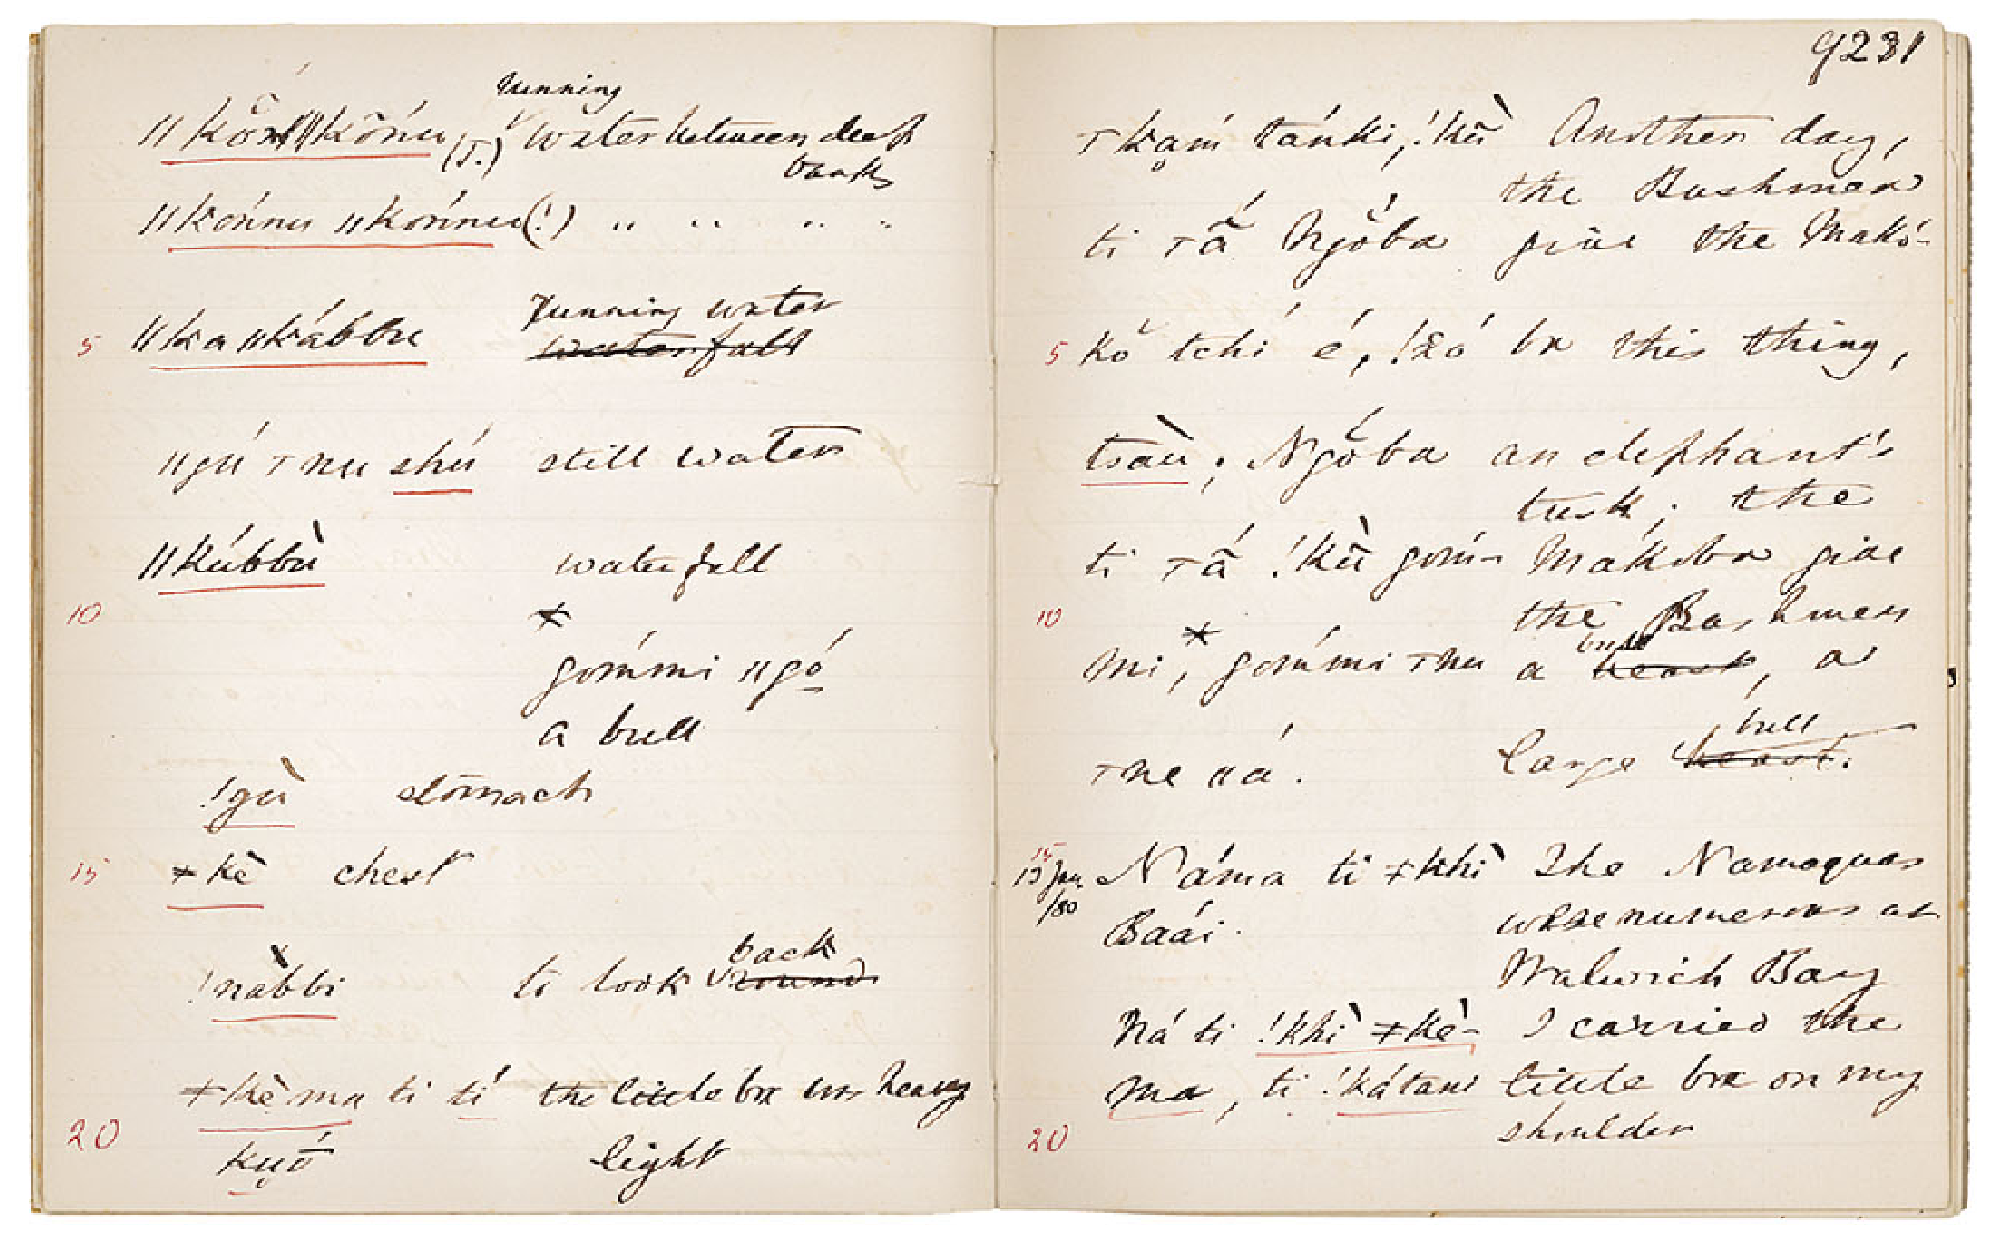
\includegraphics[width=0.95\textwidth]{chapter06/figures/case-studies.bleek-and-lloyd.A2_1_112_09231.eps}%
}%
\caption[Screenshot showing a sample page from Bleek\& Lloyd collection]{Screenshot showing a sample page from the ``Posts and trading'' story in the Lucy Lloyd !Kun notebooks}
\label{fig:case-studies:bleek-and-lloyd:brief-history:case-studies.bleek-and-lloyd.A2_1_112_09231}
% \end{center}
\end{figure}

%%%%%\subsection[Bushman folklore]{Bushman folklore}
%%%%%\label{sec:case-studies:bleek-and-lloyd:bushman-folklore}
%%%%%\subsection[Brief history]{Brief history}
\subsection[Overview]{Overview}
\label{sec:case-studies:bleek-and-lloyd:brief-history}

The Bleek and Lloyd collection \citep{Skotnes2007} is a 19th century compilation of notebooks and drawings comprising of linguistic and ethnographic work of Lucy Lloyd and Wilhelm Bleek on the life of the \textbar Xam\index{Xam} and !Kun\index{Kun} Bushman people of Southern Africa. In 2003, the Lucy Lloyd Archive and Research centre at the University of Cape Town embarked on a large scale digitisation project and all the artifacts are in the process of being scanned and corresponding representation information generated. Table~\ref{tab:case-studies:overview:lloydbleek-database-collection} shows the current composition of the digitised objects and Figure~\ref{fig:case-studies:bleek-and-lloyd:brief-history:case-studies.bleek-and-lloyd.A2_1_112_09231} shows a sample page from one of the digitised notebooks.

%\subsection{Non-Functional Requirements}
%\label{sec:design-implementation:design-process:non-functional-requirements}
%http://upload.wikimedia.org/wikipedia/commons/2/2b/Data_modeling_context.svg

%\begin{comment}
% PLEASE SEE PAGE 51---overview of strategies table
%
%http://jeffrey.famvdhoeven.nl/Researchtask%20IBM%20TU%20Delft%20-%20J.R.%20van%
%20der%20Hoeven.pdf
%\end{comment}

%Nice table outline here
%(\url{
%http://www.slideshare.net/henry.muccini/software-architecture-design-decisions}
%)
%Questions
%Options
%criteria

\tablespacing
%%%%%\begin{longtable}{p{0.4\linewidth} p{0.5\linewidth}}
\begin{longtable}{
>{\arraybackslash}p{0.30\linewidth}|
>{\arraybackslash}p{0.60\linewidth}}

\caption{Bleek\& Lloyd collection profile}
\label{tab:case-studies:overview:lloydbleek-database-collection} \\

 %%%%%%\toprule
 %%%%%\textbf{} & \textbf{}\\
 %%%%%\cline{1-2}
 \endfirsthead

 \caption[]{(continued)}\\
 %%%%%%\toprule
 %%%%%\textbf{} & \textbf{}\\
 %%%%%\cline{1-2}
 \endhead

 % Page footer
 \midrule
 \multicolumn{2}{r}{(Continued on next page)} \\
 \endfoot

 % Last page footer
 %%%%%%\bottomrule
 \endlastfoot

 %%%%%{} &
 %%%%%{} \\
 %%%%%\cline{1-2}
 %\cmidrule[0.1pt](l{0.5em}r{0.5em}){1-2}

 {\textbf{Collection theme}} &
 {Historical artifacts; museum objects}\\

 \cline{1-2}
 %\cmidrule[0.1pt](l{0.5em}r{0.5em}){1-2}

 {\textbf{Media types}} &
 {Digitised}\\

 \cline{1-2}
 %\cmidrule[0.1pt](l{0.5em}r{0.5em}){1-2}

 {\textbf{Collection size}} &
 {6.2GB}\\

 \cline{1-2}
 %\cmidrule[0.1pt](l{0.5em}r{0.5em}){1-2}

 {\textbf{Content type}} &
 {image/jpeg}\\

 \cline{1-2}
 %\cmidrule[0.1pt](l{0.5em}r{0.5em}){1-2}

 {\textbf{Number of collections}} &
 {\num{6}}\\

 \cline{1-2}
 %\cmidrule[0.1pt](l{0.5em}r{0.5em}){1-2}

 {\textbf{Number of objects}} &
 {\num{18924}}\\

 %%%%%\cline{1-2}
 %\cmidrule[0.1pt](l{0.5em}r{0.5em}){1-2}

 \end{longtable}

\bodyspacing

\subsection{Object storage}
\label{sec:case-studies:bleek-and-lloyd:implementation}

\tablespacing
%%%%%\begin{longtable}{p{0.3\linewidth} p{0.6\linewidth}}
\begin{longtable}{
>{\arraybackslash}p{0.20\linewidth}|
>{\arraybackslash}p{0.25\linewidth}|
>{\arraybackslash}p{0.45\linewidth}}

\caption{Bleek\& Lloyd repository item classification}
\label{tab:case-studies:bleek-and-lloyd:object-organisation} \\

 %%%%%\toprule
 %%%%%\hline
 \textbf{Item} & 
 \textbf{Object Type} & 
 \textbf{Comments}\\
 %%%%%\midrule
 %%%%%\hline
 \cline{1-3}
 \endfirsthead

 \caption[]{(continued)}\\
 %%%%%\toprule
 %%%%%\hline
 \textbf{Item Type} & 
 \textbf{Object Type} & 
 \textbf{Comments}\\
 %%%%%\midrule
 %%%%%\hline
 \cline{1-3}
 \endhead

 % Page footer
 %%%%%\midrule
 %%%%%\hline
 \multicolumn{3}{r}{(Continued on next page)} \\
 \endfoot

 % Last page footer
 %%%%%\bottomrule
 \endlastfoot

 {\textbf{Notebook}}&
 {Container object} &
 {Author compilation of books} \\

 %%%%%\cmidrule[0.1pt](l{0.5em}r{0.5em}){1-2}
 \cline{1-3}

 {\textbf{Book}} &
 {Container object} &
 {Compilation of digitised pages} \\

 %%%%%\cmidrule[0.1pt](l{0.5em}r{0.5em}){1-2}
 \cline{1-3}

 {\textbf{Story}} &
 {Content object} &
 {Content object without bitsreams} \\

 %%%%%\cmidrule[0.1pt](l{0.5em}r{0.5em}){1-2}
 \cline{1-3}

 {\textbf{Page}} &
 {Content object} &
 {Digitised page} \\

 %%%%%\cmidrule[0.1pt](l{0.5em}r{0.5em}){1-2}
 %%%%%\cline{1-3}

 \end{longtable}

\bodyspacing

Table~\ref{tab:case-studies:bleek-and-lloyd:object-organisation} shows the object composition of the collection and Figure~\ref{fig:case-studies:bleek-and-lloyd:object-storage:object-relationships} shows the relationships among the objects.

\begin{figure}
 \centering
 \framebox[\textwidth]{
 % Generated with LaTeXDraw 2.0.8
% Sun Mar 03 17:46:51 SAST 2013
% \usepackage[usenames,dvipsnames]{pstricks}
% \usepackage{epsfig}
% \usepackage{pst-grad} % For gradients
% \usepackage{pst-plot} % For axes
\scalebox{1} % Change this value to rescale the drawing.
{
\begin{pspicture}(0,-4.24)(11.44,4.08)
\definecolor{color126b}{rgb}{0.7176470588235294,0.8862745098039215,0.9411764705882353}
\psline[linewidth=0.06cm](9.34,-2.96)(4.72,-0.64)
\psline[linewidth=0.06cm](1.76,-2.98)(6.4,-0.66)
\psline[linewidth=0.06cm](5.58,2.08)(5.58,-1.2)
\psframe[linewidth=0.06,dimen=outer,shadow=true,shadowangle=-45.0,shadowsize=0.1,fillstyle=solid,fillcolor=color126b](7.78,1.0)(3.38,-1.0)
\psframe[linewidth=0.06,dimen=outer,shadow=true,shadowangle=-45.0,shadowsize=0.1,fillstyle=solid,fillcolor=color126b](4.4,-1.8)(0.0,-3.8)
\psframe[linewidth=0.06,dimen=outer,shadow=true,shadowangle=-45.0,shadowsize=0.1,fillstyle=solid,fillcolor=color126b](7.78,3.8)(3.38,1.8)
\psframe[linewidth=0.06,dimen=outer,shadow=true,shadowangle=-45.0,shadowsize=0.1,fillstyle=solid,fillcolor=color126b](11.2,-1.8)(6.8,-3.8)
\psframe[linewidth=0.06,dimen=outer,fillstyle=solid](7.18,3.4)(3.98,2.2)
\usefont{T1}{ptm}{b}{n}
\rput(5.5692186,2.805){Notebook}
\psframe[linewidth=0.06,dimen=outer,fillstyle=solid](7.18,0.6)(3.98,-0.6)
\usefont{T1}{ptm}{b}{n}
\rput(5.6179686,0.005){Book}
\psframe[linewidth=0.06,linestyle=dashed,dash=0.16cm 0.16cm,dimen=outer,fillstyle=solid](3.82,-2.2)(0.62,-3.4)
\usefont{T1}{ptm}{b}{n}
\rput(2.1889062,-2.795){Story}
\psframe[linewidth=0.06,linestyle=dashed,dash=0.16cm 0.16cm,dimen=outer,fillstyle=solid](10.6,-2.2)(7.4,-3.4)
\usefont{T1}{ptm}{b}{n}
\rput(8.921094,-2.795){Page}
\end{pspicture} 
}


 }
 \caption{Collection digital object component structure}
 \label{fig:case-studies:bleek-and-lloyd:object-storage:object-relationships}
\end{figure}

%%%%%\subsubsection{Data model}
%%%%%\label{sec:case-studies:bleek-and-lloyd:implementation:data-model}

The metadata objects are encoded using Dublin Core \citep{DCMI1999}; Listings~\ref{lst:case-studies:bleek-and-lloyd:data-model:metadata-schema:content},~\ref{lst:case-studies:bleek-and-lloyd:data-model:metadata-schema:virtual} and~\ref{lst:case-studies:bleek-and-lloyd:data-model:metadata-schema:container} show sample encoding for Content Objects, ``virtual'' Content Objects and Container Objects.

%%%%%\subsubsection{Metadata schema}
%%%%%\label{sec:case-studies:bleek-and-lloyd:implementation:metadata-schema}

\lstinputlisting[float,frame=lines,caption=A digital content metadata file, label=lst:case-studies:bleek-and-lloyd:data-model:metadata-schema:content, language=XML]{chapter06/code/code.case-studies.bleek-and-lloyd.digital-content.metadata}

\lstinputlisting[float,frame=lines, caption=A virtual object metadata file, label=lst:case-studies:bleek-and-lloyd:data-model:metadata-schema:virtual,language=XML]{chapter06/code/code.case-studies.bleek-and-lloyd.virtual-object.metadata}

\lstinputlisting[float,frame=lines,caption=A container object metadata file,label=lst:case-studies:bleek-and-lloyd:data-model:metadata-schema:container,language=XML]{chapter06/code/code.case-studies.bleek-and-lloyd.container-object.metadata }

\subsection[DLSes]{Digital Library Systems}
\label{sec:case-studies:bleek-and-lloyd:use-cases}

\subsubsection{The Digital Bleek and Lloyd collection}
\label{sec:case-studies:bleek-and-lloyd:use-cases:the-digital-bleek-and-lloyd}

The digital Bleek and Lloyd collection \citep{LloydBleek2007} is an online\footnote{\url{http://lloydbleekcollection.cs.uct.ac.za}} catalogue that was developed to store and enable access to digitised manuscripts described in Section~\ref{sec:case-studies:bleek-and-lloyd:brief-history}. The underlying software was initially designed to enable access to as many people as possible so usage requirements were minimal---it was not even necessary to use a Web server or database. The system was designed to be XML-centric, and is based on an implementation strategy that involves pre-generating scalable hyperlinked XHTML pages using XSLT \citep{Suleman2007}. However, the original system was not focused on preservation, extensibility or reusability. In an attempt to take advantage of these attributes and also simplify the resulting system, a prototype redesigned system \citep{Phiri2012} was developed using the repository described in Section~\ref{sec:case-studies:bleek-and-lloyd:implementation} as the underlying data storage layer.

\subsubsection{Bonolo}
\label{sec:case-studies:bleek-and-lloyd:use-cases:bonolo}

The Bonolo project---undertaken in 2012---was initiated to investigate a new approach to building digital repository systems \citep{Hammer2011}. One of the project deliverable is a prototype generic \gls{dls} \citep{Hammer2011, Phiri2012a} that makes use of the repository described in Section~\ref{sec:case-studies:bleek-and-lloyd:implementation} as the data storage layer.
%%%%%\section[NDLTD union catalog]{NDLTD union catalogue}\index{NDLTD}
\label{sec:case-studies:ndltd-union-catalog}

%
%
%
\subsection{OAI-PMH downstream service}
\label{sec:case-studies:ndltd-union-catalog:oaipmh-downstream-service}

xxx

 %%%%% February 22, 2013---I don't think Union catalog is real life case study
\section[SARU archaeological database]{SARU archaeological database}\index{SARU}
\label{sec:case-studies:saru-archaeological-database}

\begin{figure}
 %\begin{center}
  \centering
  \framebox[\textwidth]{%
\includegraphics[width=0.95\textwidth]{chapter06/figures/case-studies.saru.die-mond-south-plant-fossil.eps}%
}%
\caption[Screenshot showing a sample rock art from SARU collection]{Screenshot showing the Die Mond South plant fossil from the Eastern Cederberg rock art site}
\label{fig:case-studies:saru-archaeological-database:legacy-database-migration:die-mond-south-plant-fossil}
% \end{center}
\end{figure}

%\subsection{Bleek and Lloyd Collection}
%\label{sec:design-implementation:implementation-casestudies:bl}
%
%\subsection{NDLTD Union Catalog}
%\label{sec:design-implementation:implementation-casestudies:ndltd}
%
%\subsection{SARU Archaeological Database}
%\label{sec:design-implementation:implementation-casestudies:saru}
%\subsection{Spatial archaeological analysis}
%\label{sec:case-studies:saru-archaeological-database:spatial-archaeological-analysis}
%
%xxx

%%%%%\subsection{Rock art paintings}
%%%%%\label{sec:case-studies:saru-archaeological-database:rock-art-paintings}
%%%%%\subsection{Legacy database}
\subsection[Overview]{Overview}
\label{sec:case-studies:saru-archaeological-database:legacy-database-migration}

The Department of Archaeology\footnote{\url{http://web.uct.ac.za/depts/age}}'s \gls{saru} at the University of Cape Town has been compiling archaeological collections since the early 1950s. These collections are predominantly in the form of site records and corresponding artifacts within the vicinity of the sites. Table~\ref{tab:case-studies:overview:saru-database-collection} show the composition of collections that have been compiled thus far, and Figure~\ref{fig:case-studies:saru-archaeological-database:legacy-database-migration:die-mond-south-plant-fossil} shows an image of a rock art motif from one of the archaeological sites.

Owing to the growing number of collections and a growing need by a number of researchers to access this information, an archaeological database was designed in 2005, in part, to produce layers suitable for integration with Geographic Information Systems. The site records are currently accessed via a Microsoft Access\footnote{\url{http://office.microsoft.com/en-us/access}} database-based desktop application used to store the digital archive \citep{Wiltshire2011}.

\tablespacing
\begin{longtable}{
>{\arraybackslash}p{0.30\linewidth}|
>{\arraybackslash}p{0.60\linewidth}}

\caption{SARU archaeological database collection profile}
\label{tab:case-studies:overview:saru-database-collection} \\

 %%%%%%\toprule
 %%%%%\textbf{} & \textbf{}\\
 %%%%%\cline{1-2}
 \endfirsthead

 \caption[]{(continued)}\\
 %%%%%%\toprule
 %%%%%\textbf{} & \textbf{}\\
 %%%%%\cline{1-2}
 \endhead

 % Page footer
 \midrule
 \multicolumn{2}{r}{(Continued on next page)} \\
 \endfoot

 % Last page footer
 %%%%%%\bottomrule
 \endlastfoot

 
 %%%%%{} & 
 %%%%%{} \\
 %\cmidrule[0.1pt](l{0.5em}r{0.5em}){1-2}
 %%%%%\cline{1-2}

 {\textbf{Collection theme}}&
 {Archaeology artifacts; museum objects}\\

 \cline{1-2}
 %\cmidrule[0.1pt](l{0.5em}r{0.5em}){1-2}

 {\textbf{Media types}}&
 {Born digital}\\

 \cline{1-2}
 %\cmidrule[0.1pt](l{0.5em}r{0.5em}){1-2}

 {\textbf{Collection size}}&
 {283GB}\\

 \cline{1-2}
 %\cmidrule[0.1pt](l{0.5em}r{0.5em}){1-2}

 {\textbf{Content type}}&
 {image/jpeg; image/tiff}\\

 \cline{1-2}
 %\cmidrule[0.1pt](l{0.5em}r{0.5em}){1-2}

 {\textbf{Number of collections}}&
 {\num{110}}\\

 \cline{1-2}
 %\cmidrule[0.1pt](l{0.5em}r{0.5em}){1-2}

 {\textbf{Number of objects}}&
 {\num{72333}}\\

 %%%%%\cline{1-2}
 %\cmidrule[0.1pt](l{0.5em}r{0.5em}){1-2}

 \end{longtable}

\bodyspacing

\subsection{Object storage}
\label{sec:case-studies:saru-archaeological-database:implementation}

%%%%%\subsubsection{Data model}
%%%%%\label{sec:case-studies:saru-archaeological-database:implementation:data-model}

The records from the database were re-organised to conform to the design described in Chapter~\ref{ch:implementation}. Table~\ref{tab:case-studies:saru:object-organisation} shows the object types identified in the collection and Figure~\ref{fig:case-studies:saru-storage:object-relationships} is an illustration of the repository structure and relationships among the objects. 

\tablespacing
%%%%%\begin{longtable}{p{0.3\linewidth} p{0.6\linewidth}}
\begin{longtable}{
>{\arraybackslash}p{0.25\linewidth}|
>{\arraybackslash}p{0.25\linewidth}|
>{\arraybackslash}p{0.40\linewidth}}

\caption{SARU repository item classification}
\label{tab:case-studies:saru:object-organisation} \\

 %%%%%\toprule
 %%%%%\hline
 \textbf{Item} & 
 \textbf{Object Type} & 
 \textbf{Comments}\\
 %%%%%\midrule
 %%%%%\hline
 \cline{1-3}
 \endfirsthead

 \caption[]{(continued)}\\
 %%%%%\toprule
 %%%%%\hline
 \textbf{Item Type} & 
 \textbf{Object Type} & 
 \textbf{Comments}\\
 %%%%%\midrule
 %%%%%\hline
 \cline{1-3}
 \endhead

 % Page footer
 %%%%%\midrule
 %%%%%\hline
 \multicolumn{3}{r}{(Continued on next page)} \\
 \endfoot

 % Last page footer
 %%%%%\bottomrule
 \endlastfoot

 {\textbf{Map Sheet}}&
 {Container Object} &
 {Map sheet code} \\

 %%%%%\cmidrule[0.1pt](l{0.5em}r{0.5em}){1-2}
 \cline{1-3}

 {\textbf{Farm/Kloof}} &
 {Container Object} &
 {Farm/Kloof} \\

 %%%%%\cmidrule[0.1pt](l{0.5em}r{0.5em}){1-2}
 \cline{1-3}

 {\textbf{Site Number}} &
 {Container Object} &
 {Site number} \\

 %%%%%\cmidrule[0.1pt](l{0.5em}r{0.5em}){1-2}
 \cline{1-3}

 {\textbf{Project/Recorder}} &
 {Container object} &
 {Project, recorder or contributor} \\

 %%%%%\cmidrule[0.1pt](l{0.5em}r{0.5em}){1-2}
 \cline{1-3}

 {\textbf{Artifact}} &
 {Content object} &
 {Photograph} \\

 %%%%%\cmidrule[0.1pt](l{0.5em}r{0.5em}){1-2}
 %%%%%\cline{1-3}


 \end{longtable}

\bodyspacing

The metadata records were encoded using a custom tailored metadata scheme, conforming to the original format of data input forms used by research when conducting field studies. Listings ~\ref{lst:case-studies:saru-archaeological-database:container} and ~\ref{lst:case-studies:saru-archaeological-database:site-record} show encoding for a sample site record Container object and Content object, respectively.

%%%%%\subsubsection{Metadata schema}
%%%%%\label{sec:case-studies:saru-archaeological-database:implementation:metadata-schema}

\begin{figure}
 \centering
 \framebox[\textwidth]{
 % Generated with LaTeXDraw 2.0.8
% Sun Mar 03 17:47:15 SAST 2013
% \usepackage[usenames,dvipsnames]{pstricks}
% \usepackage{epsfig}
% \usepackage{pst-grad} % For gradients
% \usepackage{pst-plot} % For axes
\scalebox{1} % Change this value to rescale the drawing.
{
\begin{pspicture}(0,-6.88)(14.68,6.82)
\definecolor{color586b}{rgb}{0.7176470588235294,0.8862745098039215,0.9411764705882353}
\psline[linewidth=0.06cm](8.76,-0.58)(3.3,-2.02)
\psline[linewidth=0.06cm](5.6,-0.56)(11.2,-2.08)
\psline[linewidth=0.06cm](7.2,4.6)(7.2,-6.2)
\psframe[linewidth=0.06,dimen=outer,shadow=true,shadowangle=-45.0,shadowsize=0.1,fillstyle=solid,fillcolor=color586b](9.4,3.8)(5.0,1.8)
\psframe[linewidth=0.06,dimen=outer,shadow=true,shadowangle=-45.0,shadowsize=0.1,fillstyle=solid,fillcolor=color586b](9.4,1.0)(5.0,-1.0)
\psframe[linewidth=0.06,dimen=outer,shadow=true,shadowangle=-45.0,shadowsize=0.1,fillstyle=solid,fillcolor=color586b](9.4,6.6)(5.0,4.6)
\psframe[linewidth=0.06,dimen=outer,shadow=true,shadowangle=-45.0,shadowsize=0.1,fillstyle=solid,fillcolor=color586b](9.4,-1.8)(5.0,-3.8)
\psframe[linewidth=0.06,dimen=outer,fillstyle=solid](8.8,6.2)(5.6,5.0)
\usefont{T1}{ptm}{b}{n}
\rput(7.224531,5.605){Map Sheet}
\psframe[linewidth=0.06,dimen=outer,fillstyle=solid](8.8,3.4)(5.6,2.2)
\usefont{T1}{ptm}{b}{n}
\rput(7.2592187,2.805){Kloof}
\psframe[linewidth=0.06,dimen=outer,fillstyle=solid](8.8,0.6)(5.6,-0.6)
\usefont{T1}{ptm}{b}{n}
\rput(7.17625,0.005){Site}
\psframe[linewidth=0.06,dimen=outer,fillstyle=solid](8.8,-2.2)(5.6,-3.4)
\usefont{T1}{ptm}{b}{n}
\rput(7.1535935,-2.835){Project}
\psframe[linewidth=0.06,dimen=outer,shadow=true,shadowangle=-45.0,shadowsize=0.1,fillstyle=solid,fillcolor=color586b](9.4,-4.6)(5.0,-6.6)
\psframe[linewidth=0.06,linestyle=dashed,dash=0.16cm 0.16cm,dimen=outer,fillstyle=solid](8.8,-5.0)(5.6,-6.2)
\usefont{T1}{ptm}{b}{n}
\rput(7.1967187,-5.595){Artifact}
\psframe[linewidth=0.06,dimen=outer,shadow=true,shadowangle=-45.0,shadowsize=0.1,fillstyle=solid,fillcolor=color586b](14.4,-1.84)(10.0,-3.84)
\psframe[linewidth=0.06,dimen=outer,fillstyle=solid](13.8,-2.24)(10.6,-3.44)
\usefont{T1}{ptm}{b}{n}
\rput(12.313907,-2.835){Recorder}
\psframe[linewidth=0.06,dimen=outer,shadow=true,shadowangle=-45.0,shadowsize=0.1,fillstyle=solid,fillcolor=color586b](4.4,-1.84)(0.0,-3.84)
\psframe[linewidth=0.06,dimen=outer,fillstyle=solid](3.8,-2.24)(0.6,-3.44)
\usefont{T1}{ptm}{b}{n}
\rput(2.24,-2.835){Contributor}
\end{pspicture} 
}


 }
 \caption{Collection digital object component structure}
 \label{fig:case-studies:saru-storage:object-relationships}
\end{figure}

\lstinputlisting[float,frame=lines,caption=A sample kloof/farm container object metadata file,label=lst:case-studies:saru-archaeological-database:container,language=XML]{chapter06/code/code.case-studies.saru.container-object.metadata}

\lstinputlisting[float,frame=lines,caption=A sample site record content object metadata file,label=lst:case-studies:saru-archaeological-database:site-record,language=XML]{chapter06/code/code.case-studies.saru.digital-content.metadata}

\subsection[DLSes]{Digital Library Systems}
\label{sec:case-studies:saru-archaeological-database:use-cases}

\subsubsection{School of rock art}
\label{sec:case-studie :saru-archaeological-database:use-cases:school-of-rock-art}

The School of Rock Art \citep{Crawford2012} is a Web application that was developed to act as an archaeology educational tool for elementary school students. The Web application is composed of three independent modules that all interact with the repository described in this section.

\section[Summary]{Summary}
\label{sec:case-studies:summary}

This chapter presented two real-world case study collections based on the simple prototype repository design outlined in Chapter~\ref{ch:implementation}. Furthermore, some \gls{dls} implementations that used each of the case study collections as repository sub-layers were highlighted.

In essence, the case studies serve as proof of concept implementations for real-world practical application of the simple design. In Chapter~\ref{ch:evaluation}, Section~\ref{sec:evaluation:developer-survey}, a user study, in the form of a developer-oriented survey that used the Bleek and Lloyd collection as the primary storage layer, is described.

\chapter{Evaluation\label{ch:evaluation}}

%%\section{Overview}
%%\label{sec:evaluation-overview}
Evaluation of \glspl{dl}\index{Digital Libraries} has been a subject of interest for \gls{dl}\index{Digital Libraries} research from the very early stages. This is evidenced by early initiatives such as the D-Lib Working Group on \gls{dl}\index{Digital Libraries} Metrics \citep{DLWG1998} that was established in the late 1990s. A series of related studies have since been conducted with the aim of outlining a systematic and viable way of evaluating the complex, multi-faceted nature of \glspl{dl}\index{Digital Libraries} that encompasses content, system and user-oriented aspects. For instance, the DELOS\index{DELOS}\footnote{\url{http://www.delos.info}} Cluster on Evaluation \citep{Borgman2002,DELOSW72004}, which is perhaps the most current and comprehensive \gls{dl}\index{Digital Libraries} evaluation initiative, was initiated with the aim of addressing the different aspects of \glspl{dl}\index{Digital Libraries} evaluation.

The DELOS\index{DELOS} \gls{dl}\index{Digital Libraries} evaluation activities have yielded some significant results; in an attempt to understand the broad view of \glspl{dl}, Fuhr et al. \citep{Fuhr2001} developed a classification and evaluation scheme using four major dimensions: data/collection, system/technology, users and usage, and further produced a MetaLibrary comprising of test-beds to be used in \gls{dl}\index{Digital Libraries} evaluation. In a follow-up paper, Fuhr et al. \citep{Fuhr2007} proposed a new framework for evaluation of \glspl{dl}\index{Digital Libraries} with detailed guidelines for the evaluation process.

This research proposes simplifying the overall design of \glspl{dls}\index{Digital Library System} and more specifically designing for simplicity of management and ease of use the resulting \glspl{dls}\index{Digital Library System}. The design principles derived in Chapter~\ref{ch:exploratory-study} were used to design and implement a simple generic repository sub-layer for \glspl{dls}\index{Digital Library System}. In Chapter~\ref{ch:case-studies} three proof of concept file-based repository implementations are presented to evaluate the effectiveness of this approach. 

A developer survey, outlined in Section~\ref{sec:evaluation:developer-survey}, was conducted to assess the impact of redesigning the repository sub-layer on extensibility of implementations based on this design. 

Furthermore, owing to the fact that repositories have a potential to grow, detailed scalability performance benchmarks were conducted to assess the performance of this design strategy relative to the sizes of collections; these performance benchmarks are outlined in Section~\ref{sec:evaluation:performance}.
\section[Developer survey]{Developer survey}
\label{sec:evaluation:developer-survey}

%\subsection{User Study}
%\label{sec:evaluation:developer-survey}

The developer-oriented user study was conducted to assess the simplicity\index{Simplicity} of file-based repository\index{Repository} implementations and the easy of interaction with such implementations.

\subsection{Target population}
\label{sec:evaluation:developer-survey:target-population}

The survey participants were recruited from a total of \num{34} Computer Science Honours (CSC4000) students, enrolled for the \gls{www}\index{WWW} elective course module at the University of Cape Town.

The \gls{www}\index{WWW} module had a mandatory practical assignment, accounting for \SI{20}{\percent} of the overall assessment, in which the students were required to build generic Web\index{Web} applications, in groups, using the file-based repository store described in Section~\ref{sec:case-studies:bleek-and-lloyd}. Screenshots of the online questionnaire are in the Appendix section\footnote{Please see Appendix~\ref{ch:appendex-b:developer-survey:questionnaire-design} for details}, and show the assignment question. A request for survey participation was emailed to the class mailing list after the assignment due date, in which \num{26} out of the \num{34} students responded, as shown in Table~\ref{tab:experimentation:survey:target-population}

\tablespacing
%%%%%\begin{longtable}{p{0.15\linewidth} p{0.035\linewidth}
%%%%%p{0.035\linewidth} p{0.035\linewidth} p{0.035\linewidth} p{0.035\linewidth}
%%%%%p{0.035\linewidth} p{0.035\linewidth} p{0.035\linewidth} p{0.035\linewidth}
%%%%%p{0.035\linewidth} p{0.035\linewidth} p {0.035\linewidth}}
\begin{longtable}{
>{\arraybackslash}p{0.18\linewidth}|
>{\centering\arraybackslash}p{0.035\linewidth}|
>{\centering\arraybackslash}p{0.035\linewidth}|
>{\centering\arraybackslash}p{0.035\linewidth}|
>{\centering\arraybackslash}p{0.035\linewidth}|
>{\centering\arraybackslash}p{0.035\linewidth}|
>{\centering\arraybackslash}p{0.035\linewidth}|
>{\centering\arraybackslash}p{0.035\linewidth}|
>{\centering\arraybackslash}p{0.035\linewidth}|
>{\centering\arraybackslash}p{0.035\linewidth}|
>{\centering\arraybackslash}p{0.035\linewidth}|
>{\centering\arraybackslash}p{0.035\linewidth}|
>{\centering\arraybackslash}p{0.035\linewidth}}


\caption{Developer survey target population}
\label{tab:experimentation:survey:target-population}\\
 %%%%%\toprule
 %%%%%\cline{2-13}
 %%{} & \multicolumn{11}{c}{\textbf{Practical Assignment Group}}\\
 %%\midrule
 \textbf{} & 
 \multicolumn{1}{c|}{\begin{sideways}\textbf{Group 1}\end{sideways}} &
 \multicolumn{1}{c|}{\begin{sideways}\textbf{Group 2}\end{sideways}} &
 \multicolumn{1}{c|}{\begin{sideways}\textbf{Group 3}\end{sideways}} &
 \multicolumn{1}{c|}{\begin{sideways}\textbf{Group 4}\end{sideways}} &
 \multicolumn{1}{c|}{\begin{sideways}\textbf{Group 5}\end{sideways}} &
 \multicolumn{1}{c|}{\begin{sideways}\textbf{Group 6}\end{sideways}} &
 \multicolumn{1}{c|}{\begin{sideways}\textbf{Group 7}\end{sideways}} &
 \multicolumn{1}{c|}{\begin{sideways}\textbf{Group 8}\end{sideways}} &
 \multicolumn{1}{c|}{\begin{sideways}\textbf{Group 9}\end{sideways}} &
 \multicolumn{1}{c|}{\begin{sideways}\textbf{Group 10}\end{sideways}} &
 \multicolumn{1}{c|}{\begin{sideways}\textbf{Group 11}\end{sideways}} &
 \multicolumn{1}{c}{\begin{sideways}\textbf{Group 12}\end{sideways}}\\
 %%%%%\midrule
 \cline{1-13}
 \endfirsthead
 
 \caption[]{(continued)}\\
 %%%%%\toprule
 %%%%%\cline{2-13}
 %%{} & \multicolumn{12}{c}{\textbf{Programming Group}}\\
 %%\midrule
 \textbf{} & 
 \multicolumn{1}{c|}{\begin{sideways}\textbf{Group 1}\end{sideways}} &
 \multicolumn{1}{c|}{\begin{sideways}\textbf{Group 2}\end{sideways}} &
 \multicolumn{1}{c|}{\begin{sideways}\textbf{Group 3}\end{sideways}} &
 \multicolumn{1}{c|}{\begin{sideways}\textbf{Group 4}\end{sideways}} &
 \multicolumn{1}{c|}{\begin{sideways}\textbf{Group 5}\end{sideways}} &
 \multicolumn{1}{c|}{\begin{sideways}\textbf{Group 6}\end{sideways}} &
 \multicolumn{1}{c|}{\begin{sideways}\textbf{Group 7}\end{sideways}} &
 \multicolumn{1}{c|}{\begin{sideways}\textbf{Group 8}\end{sideways}} &
 \multicolumn{1}{c|}{\begin{sideways}\textbf{Group 9}\end{sideways}} &
 \multicolumn{1}{c|}{\begin{sideways}\textbf{Group 10}\end{sideways}} &
 \multicolumn{1}{c|}{\begin{sideways}\textbf{Group 11}\end{sideways}} &
 \multicolumn{1}{c}{\begin{sideways}\textbf{Group 12}\end{sideways}} \\
 %%%%%\midrule
 \cline{1-13}
 \endhead
 
 % Page footer
 %%%%%\midrule
 \cline{1-13}
 \multicolumn{9}{r}{(Continued on next page)} \\
 \endfoot
 
 % Last page footer
 %%%%%\bottomrule
 \endlastfoot
 
 %   &
 \textbf{Candidates}& {3}& {3}& {3}& {3}& {3}& {2}& {3}& {3}& {3}& {3}& {3}& {2}\\
 
 \cline{1-13}
 %\cmidrule[0.1pt](l{0.5em}r{0.5em}){1-13}
 
 %  &
 \textbf{Respondents}& {3}& {3}& {1}& {2}& {2}& {3}& {3}& {1}& {2}& {2}& {1}& {2}\\
 
 %\cmidrule[0.1pt](l{0.5em}r{0.5em}){1-13}
 
\end{longtable}

\bodyspacing

\subsection{Data collection}
\label{sec:evaluation:developer-survey:data-collection}

A post-experiment survey was conducted in the form of an online questionnaire\footnote{Please see to Appendix~\ref{ch:appendex-b:developer-survey:questionnaire-design} for details}, designed using LimeSurvey\footnote{\url{http://www.limesurvey.org}}\index{LimeSurvey}. The questionnaire was aimed at eliciting participants' experience in working with a file-based collection.

\begin{figure}
 \centering
 \framebox[\textwidth]{
 % Created by tikzDevice version 0.6.2-92-0ad2792 on 2013-04-07 18:12:23
% !TEX encoding = UTF-8 Unicode
\begin{tikzpicture}[x=1pt,y=1pt]
\definecolor[named]{fillColor}{rgb}{1.00,1.00,1.00}
\path[use as bounding box,fill=fillColor,fill opacity=0.00] (0,0) rectangle (397.48,252.94);
\begin{scope}
\path[clip] (  0.00,  0.00) rectangle (397.48,252.94);
\definecolor[named]{drawColor}{rgb}{1.00,1.00,1.00}
\definecolor[named]{fillColor}{rgb}{0.90,0.90,0.90}

\path[draw=drawColor,line width= 0.6pt,line join=round,line cap=round,fill=fillColor] (  0.00,  0.00) rectangle (397.48,252.95);
\end{scope}
\begin{scope}
\path[clip] ( 77.04, 62.05) rectangle (383.26,226.50);
\definecolor[named]{fillColor}{rgb}{1.00,1.00,1.00}

\path[fill=fillColor] ( 77.04, 62.05) rectangle (383.26,226.50);
\definecolor[named]{drawColor}{rgb}{0.95,0.95,0.95}

\path[draw=drawColor,line width= 0.3pt,line join=round] (117.73, 62.05) --
	(117.73,226.50);

\path[draw=drawColor,line width= 0.3pt,line join=round] (171.26, 62.05) --
	(171.26,226.50);

\path[draw=drawColor,line width= 0.3pt,line join=round] (224.80, 62.05) --
	(224.80,226.50);

\path[draw=drawColor,line width= 0.3pt,line join=round] (278.33, 62.05) --
	(278.33,226.50);

\path[draw=drawColor,line width= 0.3pt,line join=round] (331.87, 62.05) --
	(331.87,226.50);
\definecolor[named]{drawColor}{rgb}{0.90,0.90,0.90}

\path[draw=drawColor,line width= 0.6pt,line join=round] ( 77.04, 85.54) --
	(383.26, 85.54);

\path[draw=drawColor,line width= 0.6pt,line join=round] ( 77.04,124.69) --
	(383.26,124.69);

\path[draw=drawColor,line width= 0.6pt,line join=round] ( 77.04,163.85) --
	(383.26,163.85);

\path[draw=drawColor,line width= 0.6pt,line join=round] ( 77.04,203.00) --
	(383.26,203.00);

\path[draw=drawColor,line width= 0.6pt,line join=round] ( 90.96, 62.05) --
	( 90.96,226.50);

\path[draw=drawColor,line width= 0.6pt,line join=round] (144.50, 62.05) --
	(144.50,226.50);

\path[draw=drawColor,line width= 0.6pt,line join=round] (198.03, 62.05) --
	(198.03,226.50);

\path[draw=drawColor,line width= 0.6pt,line join=round] (251.56, 62.05) --
	(251.56,226.50);

\path[draw=drawColor,line width= 0.6pt,line join=round] (305.10, 62.05) --
	(305.10,226.50);

\path[draw=drawColor,line width= 0.6pt,line join=round] (358.63, 62.05) --
	(358.63,226.50);
\definecolor[named]{fillColor}{rgb}{0.33,0.46,0.18}

\path[fill=fillColor] ( 90.96, 70.86) rectangle (230.15,100.22);
\definecolor[named]{fillColor}{rgb}{0.10,0.28,0.44}

\path[fill=fillColor] (230.15, 70.86) rectangle (347.93,100.22);
\definecolor[named]{fillColor}{rgb}{0.56,0.21,0.23}

\path[fill=fillColor] (347.93, 70.86) rectangle (358.63,100.22);
\definecolor[named]{fillColor}{rgb}{0.89,0.49,0.00}

\path[fill=fillColor] (358.63, 70.86) rectangle (369.34,100.22);
\definecolor[named]{fillColor}{rgb}{0.33,0.46,0.18}

\path[fill=fillColor] ( 90.96,110.01) rectangle (144.50,139.38);
\definecolor[named]{fillColor}{rgb}{0.10,0.28,0.44}

\path[fill=fillColor] (144.50,110.01) rectangle (347.93,139.38);
\definecolor[named]{fillColor}{rgb}{0.56,0.21,0.23}

\path[fill=fillColor] (347.93,110.01) rectangle (358.63,139.38);
\definecolor[named]{fillColor}{rgb}{0.89,0.49,0.00}

\path[fill=fillColor] (358.63,110.01) rectangle (369.34,139.38);
\definecolor[named]{fillColor}{rgb}{0.33,0.46,0.18}

\path[fill=fillColor] ( 90.96,149.17) rectangle (240.86,178.53);
\definecolor[named]{fillColor}{rgb}{0.10,0.28,0.44}

\path[fill=fillColor] (240.86,149.17) rectangle (347.93,178.53);
\definecolor[named]{fillColor}{rgb}{0.56,0.21,0.23}

\path[fill=fillColor] (347.93,149.17) rectangle (358.63,178.53);
\definecolor[named]{fillColor}{rgb}{0.89,0.49,0.00}

\path[fill=fillColor] (358.63,149.17) rectangle (369.34,178.53);
\definecolor[named]{fillColor}{rgb}{0.33,0.46,0.18}

\path[fill=fillColor] ( 90.96,188.32) rectangle (219.44,217.69);
\definecolor[named]{fillColor}{rgb}{0.10,0.28,0.44}

\path[fill=fillColor] (219.44,188.32) rectangle (358.63,217.69);
\definecolor[named]{fillColor}{rgb}{0.56,0.21,0.23}

\path[fill=fillColor] (358.63,188.32) rectangle (369.34,217.69);
\definecolor[named]{fillColor}{rgb}{0.89,0.49,0.00}

\path[fill=fillColor] (369.34,188.32) rectangle (369.34,217.69);
\end{scope}
\begin{scope}
\path[clip] (  0.00,  0.00) rectangle (397.48,252.94);
\definecolor[named]{fillColor}{rgb}{0.80,0.80,0.80}

\path[fill=fillColor] ( 77.04,226.50) rectangle (383.26,238.72);
\definecolor[named]{drawColor}{rgb}{0.00,0.00,0.00}

\node[text=drawColor,anchor=base,inner sep=0pt, outer sep=0pt, scale=  0.90] at (230.15,229.51) {Technologies background};
\end{scope}
\begin{scope}
\path[clip] (  0.00,  0.00) rectangle (397.48,252.94);
\definecolor[named]{drawColor}{rgb}{0.50,0.50,0.50}

\node[text=drawColor,anchor=base east,inner sep=0pt, outer sep=0pt, scale=  0.80] at ( 69.93, 82.79) {DB apps};

\node[text=drawColor,anchor=base east,inner sep=0pt, outer sep=0pt, scale=  0.80] at ( 69.93,121.94) {DBMS};

\node[text=drawColor,anchor=base east,inner sep=0pt, outer sep=0pt, scale=  0.80] at ( 69.93,161.09) {Web apps};

\node[text=drawColor,anchor=base east,inner sep=0pt, outer sep=0pt, scale=  0.80] at ( 69.93,200.25) {XML};
\end{scope}
\begin{scope}
\path[clip] (  0.00,  0.00) rectangle (397.48,252.94);
\definecolor[named]{drawColor}{rgb}{0.50,0.50,0.50}

\path[draw=drawColor,line width= 0.6pt,line join=round] ( 90.96, 57.78) --
	( 90.96, 62.05);

\path[draw=drawColor,line width= 0.6pt,line join=round] (144.50, 57.78) --
	(144.50, 62.05);

\path[draw=drawColor,line width= 0.6pt,line join=round] (198.03, 57.78) --
	(198.03, 62.05);

\path[draw=drawColor,line width= 0.6pt,line join=round] (251.56, 57.78) --
	(251.56, 62.05);

\path[draw=drawColor,line width= 0.6pt,line join=round] (305.10, 57.78) --
	(305.10, 62.05);

\path[draw=drawColor,line width= 0.6pt,line join=round] (358.63, 57.78) --
	(358.63, 62.05);
\end{scope}
\begin{scope}
\path[clip] (  0.00,  0.00) rectangle (397.48,252.94);
\definecolor[named]{drawColor}{rgb}{0.50,0.50,0.50}

\node[text=drawColor,anchor=base,inner sep=0pt, outer sep=0pt, scale=  0.80] at ( 90.96, 49.42) {0};

\node[text=drawColor,anchor=base,inner sep=0pt, outer sep=0pt, scale=  0.80] at (144.50, 49.42) {5};

\node[text=drawColor,anchor=base,inner sep=0pt, outer sep=0pt, scale=  0.80] at (198.03, 49.42) {10};

\node[text=drawColor,anchor=base,inner sep=0pt, outer sep=0pt, scale=  0.80] at (251.56, 49.42) {15};

\node[text=drawColor,anchor=base,inner sep=0pt, outer sep=0pt, scale=  0.80] at (305.10, 49.42) {20};

\node[text=drawColor,anchor=base,inner sep=0pt, outer sep=0pt, scale=  0.80] at (358.63, 49.42) {25};
\end{scope}
\begin{scope}
\path[clip] (  0.00,  0.00) rectangle (397.48,252.94);
\definecolor[named]{drawColor}{rgb}{0.00,0.00,0.00}

\node[text=drawColor,anchor=base,inner sep=0pt, outer sep=0pt, scale=  1.00] at (230.15, 31.70) {Number of subjects};
\end{scope}
\begin{scope}
\path[clip] (  0.00,  0.00) rectangle (397.48,252.94);
\definecolor[named]{drawColor}{rgb}{0.00,0.00,0.00}

\node[text=drawColor,rotate= 90.00,anchor=base,inner sep=0pt, outer sep=0pt, scale=  1.00] at ( 18.80,144.27) {Technologies};
\end{scope}
\begin{scope}
\path[clip] (  0.00,  0.00) rectangle (397.48,252.94);
\definecolor[named]{fillColor}{rgb}{0.90,0.90,0.90}

\path[fill=fillColor] (111.64,  9.15) rectangle (348.66, 27.65);
\end{scope}
\begin{scope}
\path[clip] (  0.00,  0.00) rectangle (397.48,252.94);
\definecolor[named]{drawColor}{rgb}{1.00,1.00,1.00}
\definecolor[named]{fillColor}{rgb}{1.00,1.00,1.00}

\path[draw=drawColor,line width= 0.6pt,line join=round,line cap=round,fill=fillColor] (119.52, 13.42) rectangle (133.97, 23.38);
\end{scope}
\begin{scope}
\path[clip] (  0.00,  0.00) rectangle (397.48,252.94);
\definecolor[named]{fillColor}{rgb}{0.33,0.46,0.18}

\path[fill=fillColor] (119.52, 13.42) rectangle (133.97, 23.38);

\path[] (119.52, 13.42) --
	(133.97, 23.38);
\end{scope}
\begin{scope}
\path[clip] (  0.00,  0.00) rectangle (397.48,252.94);
\definecolor[named]{drawColor}{rgb}{1.00,1.00,1.00}
\definecolor[named]{fillColor}{rgb}{1.00,1.00,1.00}

\path[draw=drawColor,line width= 0.6pt,line join=round,line cap=round,fill=fillColor] (174.94, 13.42) rectangle (189.39, 23.38);
\end{scope}
\begin{scope}
\path[clip] (  0.00,  0.00) rectangle (397.48,252.94);
\definecolor[named]{fillColor}{rgb}{0.10,0.28,0.44}

\path[fill=fillColor] (174.94, 13.42) rectangle (189.39, 23.38);

\path[] (174.94, 13.42) --
	(189.39, 23.38);
\end{scope}
\begin{scope}
\path[clip] (  0.00,  0.00) rectangle (397.48,252.94);
\definecolor[named]{drawColor}{rgb}{1.00,1.00,1.00}
\definecolor[named]{fillColor}{rgb}{1.00,1.00,1.00}

\path[draw=drawColor,line width= 0.6pt,line join=round,line cap=round,fill=fillColor] (231.28, 13.42) rectangle (245.74, 23.38);
\end{scope}
\begin{scope}
\path[clip] (  0.00,  0.00) rectangle (397.48,252.94);
\definecolor[named]{fillColor}{rgb}{0.56,0.21,0.23}

\path[fill=fillColor] (231.28, 13.42) rectangle (245.74, 23.38);

\path[] (231.28, 13.42) --
	(245.74, 23.38);
\end{scope}
\begin{scope}
\path[clip] (  0.00,  0.00) rectangle (397.48,252.94);
\definecolor[named]{drawColor}{rgb}{1.00,1.00,1.00}
\definecolor[named]{fillColor}{rgb}{1.00,1.00,1.00}

\path[draw=drawColor,line width= 0.6pt,line join=round,line cap=round,fill=fillColor] (287.63, 13.42) rectangle (302.09, 23.38);
\end{scope}
\begin{scope}
\path[clip] (  0.00,  0.00) rectangle (397.48,252.94);
\definecolor[named]{fillColor}{rgb}{0.89,0.49,0.00}

\path[fill=fillColor] (287.63, 13.42) rectangle (302.09, 23.38);

\path[] (287.63, 13.42) --
	(302.09, 23.38);
\end{scope}
\begin{scope}
\path[clip] (  0.00,  0.00) rectangle (397.48,252.94);
\definecolor[named]{drawColor}{rgb}{0.00,0.00,0.00}

\node[text=drawColor,anchor=base west,inner sep=0pt, outer sep=0pt, scale=  0.80] at (135.78, 15.64) {$<$ 1 year $\;\;$};
\end{scope}
\begin{scope}
\path[clip] (  0.00,  0.00) rectangle (397.48,252.94);
\definecolor[named]{drawColor}{rgb}{0.00,0.00,0.00}

\node[text=drawColor,anchor=base west,inner sep=0pt, outer sep=0pt, scale=  0.80] at (191.20, 15.64) {1-3 years $\;\;$};
\end{scope}
\begin{scope}
\path[clip] (  0.00,  0.00) rectangle (397.48,252.94);
\definecolor[named]{drawColor}{rgb}{0.00,0.00,0.00}

\node[text=drawColor,anchor=base west,inner sep=0pt, outer sep=0pt, scale=  0.80] at (247.54, 15.64) {3-6 years $\;\;$};
\end{scope}
\begin{scope}
\path[clip] (  0.00,  0.00) rectangle (397.48,252.94);
\definecolor[named]{drawColor}{rgb}{0.00,0.00,0.00}

\node[text=drawColor,anchor=base west,inner sep=0pt, outer sep=0pt, scale=  0.80] at (303.89, 15.64) {$>$ 6 years $\;\;$};
\end{scope}
\end{tikzpicture}

 }
 \caption[Survey participants' technological background]{Survey participants' background knowledge working with technologies relevant to the study.}
 \label{fig:experimentation:survey:background-technology-experience}
\end{figure}

\begin{figure}
 \centering
 \framebox[\textwidth]{
 % Created by tikzDevice version 0.6.2-92-0ad2792 on 2013-04-07 17:56:48
% !TEX encoding = UTF-8 Unicode
\begin{tikzpicture}[x=1pt,y=1pt]
\definecolor[named]{fillColor}{rgb}{1.00,1.00,1.00}
\path[use as bounding box,fill=fillColor,fill opacity=0.00] (0,0) rectangle (397.48,231.26);
\begin{scope}
\path[clip] (  0.00,  0.00) rectangle (397.48,231.26);
\definecolor[named]{drawColor}{rgb}{1.00,1.00,1.00}
\definecolor[named]{fillColor}{rgb}{0.90,0.90,0.90}

\path[draw=drawColor,line width= 0.6pt,line join=round,line cap=round,fill=fillColor] (  0.00,  0.00) rectangle (397.48,231.26);
\end{scope}
\begin{scope}
\path[clip] ( 75.16, 73.81) rectangle (383.26,204.82);
\definecolor[named]{fillColor}{rgb}{1.00,1.00,1.00}

\path[fill=fillColor] ( 75.16, 73.81) rectangle (383.26,204.82);
\definecolor[named]{drawColor}{rgb}{0.95,0.95,0.95}

\path[draw=drawColor,line width= 0.3pt,line join=round] (116.09, 73.81) --
	(116.09,204.82);

\path[draw=drawColor,line width= 0.3pt,line join=round] (169.96, 73.81) --
	(169.96,204.82);

\path[draw=drawColor,line width= 0.3pt,line join=round] (223.82, 73.81) --
	(223.82,204.82);

\path[draw=drawColor,line width= 0.3pt,line join=round] (277.68, 73.81) --
	(277.68,204.82);

\path[draw=drawColor,line width= 0.3pt,line join=round] (331.55, 73.81) --
	(331.55,204.82);
\definecolor[named]{drawColor}{rgb}{0.90,0.90,0.90}

\path[draw=drawColor,line width= 0.6pt,line join=round] ( 75.16, 98.38) --
	(383.26, 98.38);

\path[draw=drawColor,line width= 0.6pt,line join=round] ( 75.16,139.31) --
	(383.26,139.31);

\path[draw=drawColor,line width= 0.6pt,line join=round] ( 75.16,180.25) --
	(383.26,180.25);

\path[draw=drawColor,line width= 0.6pt,line join=round] ( 89.16, 73.81) --
	( 89.16,204.82);

\path[draw=drawColor,line width= 0.6pt,line join=round] (143.02, 73.81) --
	(143.02,204.82);

\path[draw=drawColor,line width= 0.6pt,line join=round] (196.89, 73.81) --
	(196.89,204.82);

\path[draw=drawColor,line width= 0.6pt,line join=round] (250.75, 73.81) --
	(250.75,204.82);

\path[draw=drawColor,line width= 0.6pt,line join=round] (304.62, 73.81) --
	(304.62,204.82);

\path[draw=drawColor,line width= 0.6pt,line join=round] (358.48, 73.81) --
	(358.48,204.82);
\definecolor[named]{fillColor}{rgb}{0.33,0.46,0.18}

\path[fill=fillColor] ( 89.16, 83.02) rectangle (229.21,113.73);
\definecolor[named]{fillColor}{rgb}{0.89,0.49,0.00}

\path[fill=fillColor] (229.21, 83.02) rectangle (315.39,113.73);
\definecolor[named]{fillColor}{rgb}{0.43,0.56,0.52}

\path[fill=fillColor] (315.39, 83.02) rectangle (369.25,113.73);
\definecolor[named]{fillColor}{rgb}{0.56,0.21,0.23}

\path[fill=fillColor] (369.25, 83.02) rectangle (369.25,113.73);
\definecolor[named]{fillColor}{rgb}{0.10,0.28,0.44}

\path[fill=fillColor] (369.25, 83.02) rectangle (369.25,113.73);
\definecolor[named]{fillColor}{rgb}{0.33,0.46,0.18}

\path[fill=fillColor] ( 89.16,123.96) rectangle ( 89.16,154.67);
\definecolor[named]{fillColor}{rgb}{0.89,0.49,0.00}

\path[fill=fillColor] ( 89.16,123.96) rectangle (143.02,154.67);
\definecolor[named]{fillColor}{rgb}{0.43,0.56,0.52}

\path[fill=fillColor] (143.02,123.96) rectangle (250.75,154.67);
\definecolor[named]{fillColor}{rgb}{0.56,0.21,0.23}

\path[fill=fillColor] (250.75,123.96) rectangle (326.16,154.67);
\definecolor[named]{fillColor}{rgb}{0.10,0.28,0.44}

\path[fill=fillColor] (326.16,123.96) rectangle (369.25,154.67);
\definecolor[named]{fillColor}{rgb}{0.33,0.46,0.18}

\path[fill=fillColor] ( 89.16,164.90) rectangle ( 99.93,195.61);
\definecolor[named]{fillColor}{rgb}{0.89,0.49,0.00}

\path[fill=fillColor] ( 99.93,164.90) rectangle (153.80,195.61);
\definecolor[named]{fillColor}{rgb}{0.43,0.56,0.52}

\path[fill=fillColor] (153.80,164.90) rectangle (239.98,195.61);
\definecolor[named]{fillColor}{rgb}{0.56,0.21,0.23}

\path[fill=fillColor] (239.98,164.90) rectangle (304.62,195.61);
\definecolor[named]{fillColor}{rgb}{0.10,0.28,0.44}

\path[fill=fillColor] (304.62,164.90) rectangle (369.25,195.61);
\end{scope}
\begin{scope}
\path[clip] (  0.00,  0.00) rectangle (397.48,231.26);
\definecolor[named]{fillColor}{rgb}{0.80,0.80,0.80}

\path[fill=fillColor] ( 75.16,204.82) rectangle (383.26,217.04);
\definecolor[named]{drawColor}{rgb}{0.00,0.00,0.00}

\node[text=drawColor,anchor=base,inner sep=0pt, outer sep=0pt, scale=  0.90] at (229.21,207.83) {Storage background};
\end{scope}
\begin{scope}
\path[clip] (  0.00,  0.00) rectangle (397.48,231.26);
\definecolor[named]{drawColor}{rgb}{0.50,0.50,0.50}

\node[text=drawColor,anchor=base east,inner sep=0pt, outer sep=0pt, scale=  0.80] at ( 68.04, 95.62) {Cloud};

\node[text=drawColor,anchor=base east,inner sep=0pt, outer sep=0pt, scale=  0.80] at ( 68.04,136.56) {Database};

\node[text=drawColor,anchor=base east,inner sep=0pt, outer sep=0pt, scale=  0.80] at ( 68.04,177.50) {File};
\end{scope}
\begin{scope}
\path[clip] (  0.00,  0.00) rectangle (397.48,231.26);
\definecolor[named]{drawColor}{rgb}{0.50,0.50,0.50}

\path[draw=drawColor,line width= 0.6pt,line join=round] ( 89.16, 69.54) --
	( 89.16, 73.81);

\path[draw=drawColor,line width= 0.6pt,line join=round] (143.02, 69.54) --
	(143.02, 73.81);

\path[draw=drawColor,line width= 0.6pt,line join=round] (196.89, 69.54) --
	(196.89, 73.81);

\path[draw=drawColor,line width= 0.6pt,line join=round] (250.75, 69.54) --
	(250.75, 73.81);

\path[draw=drawColor,line width= 0.6pt,line join=round] (304.62, 69.54) --
	(304.62, 73.81);

\path[draw=drawColor,line width= 0.6pt,line join=round] (358.48, 69.54) --
	(358.48, 73.81);
\end{scope}
\begin{scope}
\path[clip] (  0.00,  0.00) rectangle (397.48,231.26);
\definecolor[named]{drawColor}{rgb}{0.50,0.50,0.50}

\node[text=drawColor,anchor=base,inner sep=0pt, outer sep=0pt, scale=  0.80] at ( 89.16, 61.19) {0};

\node[text=drawColor,anchor=base,inner sep=0pt, outer sep=0pt, scale=  0.80] at (143.02, 61.19) {5};

\node[text=drawColor,anchor=base,inner sep=0pt, outer sep=0pt, scale=  0.80] at (196.89, 61.19) {10};

\node[text=drawColor,anchor=base,inner sep=0pt, outer sep=0pt, scale=  0.80] at (250.75, 61.19) {15};

\node[text=drawColor,anchor=base,inner sep=0pt, outer sep=0pt, scale=  0.80] at (304.62, 61.19) {20};

\node[text=drawColor,anchor=base,inner sep=0pt, outer sep=0pt, scale=  0.80] at (358.48, 61.19) {25};
\end{scope}
\begin{scope}
\path[clip] (  0.00,  0.00) rectangle (397.48,231.26);
\definecolor[named]{drawColor}{rgb}{0.00,0.00,0.00}

\node[text=drawColor,anchor=base,inner sep=0pt, outer sep=0pt, scale=  1.00] at (229.21, 43.46) {Number of subjects };
\end{scope}
\begin{scope}
\path[clip] (  0.00,  0.00) rectangle (397.48,231.26);
\definecolor[named]{drawColor}{rgb}{0.00,0.00,0.00}

\node[text=drawColor,rotate= 90.00,anchor=base,inner sep=0pt, outer sep=0pt, scale=  1.00] at ( 18.80,139.31) { Storage solutions};
\end{scope}
\begin{scope}
\path[clip] (  0.00,  0.00) rectangle (397.48,231.26);
\definecolor[named]{fillColor}{rgb}{0.90,0.90,0.90}

\path[fill=fillColor] (101.45,  9.15) rectangle (356.96, 39.41);
\end{scope}
\begin{scope}
\path[clip] (  0.00,  0.00) rectangle (397.48,231.26);
\definecolor[named]{drawColor}{rgb}{1.00,1.00,1.00}
\definecolor[named]{fillColor}{rgb}{1.00,1.00,1.00}

\path[draw=drawColor,line width= 0.6pt,line join=round,line cap=round,fill=fillColor] (109.33, 25.19) rectangle (123.79, 35.14);
\end{scope}
\begin{scope}
\path[clip] (  0.00,  0.00) rectangle (397.48,231.26);
\definecolor[named]{fillColor}{rgb}{0.33,0.46,0.18}

\path[fill=fillColor] (109.33, 25.19) rectangle (123.79, 35.14);

\path[] (109.33, 25.19) --
	(123.79, 35.14);
\end{scope}
\begin{scope}
\path[clip] (  0.00,  0.00) rectangle (397.48,231.26);
\definecolor[named]{drawColor}{rgb}{1.00,1.00,1.00}
\definecolor[named]{fillColor}{rgb}{1.00,1.00,1.00}

\path[draw=drawColor,line width= 0.6pt,line join=round,line cap=round,fill=fillColor] (176.95, 25.19) rectangle (191.40, 35.14);
\end{scope}
\begin{scope}
\path[clip] (  0.00,  0.00) rectangle (397.48,231.26);
\definecolor[named]{fillColor}{rgb}{0.89,0.49,0.00}

\path[fill=fillColor] (176.95, 25.19) rectangle (191.40, 35.14);

\path[] (176.95, 25.19) --
	(191.40, 35.14);
\end{scope}
\begin{scope}
\path[clip] (  0.00,  0.00) rectangle (397.48,231.26);
\definecolor[named]{drawColor}{rgb}{1.00,1.00,1.00}
\definecolor[named]{fillColor}{rgb}{1.00,1.00,1.00}

\path[draw=drawColor,line width= 0.6pt,line join=round,line cap=round,fill=fillColor] (225.14, 25.19) rectangle (239.59, 35.14);
\end{scope}
\begin{scope}
\path[clip] (  0.00,  0.00) rectangle (397.48,231.26);
\definecolor[named]{fillColor}{rgb}{0.43,0.56,0.52}

\path[fill=fillColor] (225.14, 25.19) rectangle (239.59, 35.14);

\path[] (225.14, 25.19) --
	(239.59, 35.14);
\end{scope}
\begin{scope}
\path[clip] (  0.00,  0.00) rectangle (397.48,231.26);
\definecolor[named]{drawColor}{rgb}{1.00,1.00,1.00}
\definecolor[named]{fillColor}{rgb}{1.00,1.00,1.00}

\path[draw=drawColor,line width= 0.6pt,line join=round,line cap=round,fill=fillColor] (290.35, 25.19) rectangle (304.81, 35.14);
\end{scope}
\begin{scope}
\path[clip] (  0.00,  0.00) rectangle (397.48,231.26);
\definecolor[named]{fillColor}{rgb}{0.56,0.21,0.23}

\path[fill=fillColor] (290.35, 25.19) rectangle (304.81, 35.14);

\path[] (290.35, 25.19) --
	(304.81, 35.14);
\end{scope}
\begin{scope}
\path[clip] (  0.00,  0.00) rectangle (397.48,231.26);
\definecolor[named]{drawColor}{rgb}{1.00,1.00,1.00}
\definecolor[named]{fillColor}{rgb}{1.00,1.00,1.00}

\path[draw=drawColor,line width= 0.6pt,line join=round,line cap=round,fill=fillColor] (109.33, 13.42) rectangle (123.79, 23.38);
\end{scope}
\begin{scope}
\path[clip] (  0.00,  0.00) rectangle (397.48,231.26);
\definecolor[named]{fillColor}{rgb}{0.10,0.28,0.44}

\path[fill=fillColor] (109.33, 13.42) rectangle (123.79, 23.38);

\path[] (109.33, 13.42) --
	(123.79, 23.38);
\end{scope}
\begin{scope}
\path[clip] (  0.00,  0.00) rectangle (397.48,231.26);
\definecolor[named]{drawColor}{rgb}{0.00,0.00,0.00}

\node[text=drawColor,anchor=base west,inner sep=0pt, outer sep=0pt, scale=  0.80] at (125.59, 27.41) {Not at all $\;\;$};
\end{scope}
\begin{scope}
\path[clip] (  0.00,  0.00) rectangle (397.48,231.26);
\definecolor[named]{drawColor}{rgb}{0.00,0.00,0.00}

\node[text=drawColor,anchor=base west,inner sep=0pt, outer sep=0pt, scale=  0.80] at (193.21, 27.41) {Rarely $\;\;$};
\end{scope}
\begin{scope}
\path[clip] (  0.00,  0.00) rectangle (397.48,231.26);
\definecolor[named]{drawColor}{rgb}{0.00,0.00,0.00}

\node[text=drawColor,anchor=base west,inner sep=0pt, outer sep=0pt, scale=  0.80] at (241.40, 27.41) {Some times $\;\;$};
\end{scope}
\begin{scope}
\path[clip] (  0.00,  0.00) rectangle (397.48,231.26);
\definecolor[named]{drawColor}{rgb}{0.00,0.00,0.00}

\node[text=drawColor,anchor=base west,inner sep=0pt, outer sep=0pt, scale=  0.80] at (306.61, 27.41) {Most times $\;\;$};
\end{scope}
\begin{scope}
\path[clip] (  0.00,  0.00) rectangle (397.48,231.26);
\definecolor[named]{drawColor}{rgb}{0.00,0.00,0.00}

\node[text=drawColor,anchor=base west,inner sep=0pt, outer sep=0pt, scale=  0.80] at (125.59, 15.64) {All the time $\;\;$};
\end{scope}
\end{tikzpicture}

 }
 \caption[Survey participants' background using storage solutions]{Survey participants' background working with some selected popular storage solutions.}
 \label{fig:experimentation:survey:background-storage-usage-frequency}
\end{figure}

\begin{figure}
 \centering
 \framebox[\textwidth]{
 % Created by tikzDevice version 0.6.2-92-0ad2792 on 2013-04-07 17:57:35
% !TEX encoding = UTF-8 Unicode
\begin{tikzpicture}[x=1pt,y=1pt]
\definecolor[named]{fillColor}{rgb}{1.00,1.00,1.00}
\path[use as bounding box,fill=fillColor,fill opacity=0.00] (0,0) rectangle (397.48,216.81);
\begin{scope}
\path[clip] (  0.00,  0.00) rectangle (397.48,216.81);
\definecolor[named]{drawColor}{rgb}{1.00,1.00,1.00}
\definecolor[named]{fillColor}{rgb}{0.90,0.90,0.90}

\path[draw=drawColor,line width= 0.6pt,line join=round,line cap=round,fill=fillColor] (  0.00,  0.00) rectangle (397.48,216.81);
\end{scope}
\begin{scope}
\path[clip] ( 86.31, 66.91) rectangle (383.26,190.36);
\definecolor[named]{fillColor}{rgb}{1.00,1.00,1.00}

\path[fill=fillColor] ( 86.31, 66.91) rectangle (383.26,190.36);
\definecolor[named]{drawColor}{rgb}{0.90,0.90,0.90}

\path[draw=drawColor,line width= 0.6pt,line join=round] ( 86.31, 90.06) --
	(383.26, 90.06);

\path[draw=drawColor,line width= 0.6pt,line join=round] ( 86.31,128.64) --
	(383.26,128.64);

\path[draw=drawColor,line width= 0.6pt,line join=round] ( 86.31,167.22) --
	(383.26,167.22);

\path[draw=drawColor,line width= 0.6pt,line join=round] (120.57, 66.91) --
	(120.57,190.36);

\path[draw=drawColor,line width= 0.6pt,line join=round] (349.00, 66.91) --
	(349.00,190.36);
\definecolor[named]{drawColor}{rgb}{0.20,0.20,0.20}
\definecolor[named]{fillColor}{rgb}{0.20,0.20,0.20}

\path[draw=drawColor,line width= 0.6pt,line join=round,fill=fillColor] (177.68, 90.06) -- (234.78, 90.06);

\path[draw=drawColor,line width= 0.6pt,line join=round,fill=fillColor] (120.57, 90.06) -- (120.57, 90.06);
\definecolor[named]{fillColor}{rgb}{0.10,0.28,0.44}

\path[draw=drawColor,line width= 0.6pt,line join=round,line cap=round,fill=fillColor] (177.68, 75.59) --
	(120.57, 75.59) --
	(120.57,104.53) --
	(177.68,104.53) --
	(177.68, 75.59) --
	cycle;
\definecolor[named]{fillColor}{rgb}{0.20,0.20,0.20}

\path[draw=drawColor,line width= 1.1pt,line join=round,fill=fillColor] (177.68, 75.59) -- (177.68,104.53);

\path[draw=drawColor,line width= 0.6pt,line join=round,fill=fillColor] (234.78,128.64) -- (291.89,128.64);

\path[draw=drawColor,line width= 0.6pt,line join=round,fill=fillColor] (120.57,128.64) -- (120.57,128.64);
\definecolor[named]{fillColor}{rgb}{0.56,0.21,0.23}

\path[draw=drawColor,line width= 0.6pt,line join=round,line cap=round,fill=fillColor] (234.78,114.17) --
	(120.57,114.17) --
	(120.57,143.10) --
	(234.78,143.10) --
	(234.78,114.17) --
	cycle;
\definecolor[named]{fillColor}{rgb}{0.20,0.20,0.20}

\path[draw=drawColor,line width= 1.1pt,line join=round,fill=fillColor] (177.68,114.17) -- (177.68,143.10);

\path[draw=drawColor,line width= 0.6pt,line join=round,fill=fillColor] (220.51,167.22) -- (234.78,167.22);

\path[draw=drawColor,line width= 0.6pt,line join=round,fill=fillColor] (120.57,167.22) -- (120.57,167.22);
\definecolor[named]{fillColor}{rgb}{0.33,0.46,0.18}

\path[draw=drawColor,line width= 0.6pt,line join=round,line cap=round,fill=fillColor] (220.51,152.75) --
	(120.57,152.75) --
	(120.57,181.68) --
	(220.51,181.68) --
	(220.51,152.75) --
	cycle;
\definecolor[named]{fillColor}{rgb}{0.20,0.20,0.20}

\path[draw=drawColor,line width= 1.1pt,line join=round,fill=fillColor] (177.68,152.75) -- (177.68,181.68);
\definecolor[named]{fillColor}{rgb}{1.00,1.00,1.00}

\path[fill=fillColor] (161.36, 90.06) --
	(166.70, 95.39) --
	(172.03, 90.06) --
	(166.70, 84.72) --
	cycle;

\path[fill=fillColor] (176.74,128.64) --
	(182.07,133.97) --
	(187.41,128.64) --
	(182.07,123.30) --
	cycle;

\path[fill=fillColor] (163.56,167.22) --
	(168.89,172.55) --
	(174.23,167.22) --
	(168.89,161.88) --
	cycle;
\end{scope}
\begin{scope}
\path[clip] (  0.00,  0.00) rectangle (397.48,216.81);
\definecolor[named]{fillColor}{rgb}{0.80,0.80,0.80}

\path[fill=fillColor] ( 86.31,190.36) rectangle (383.26,202.58);
\definecolor[named]{drawColor}{rgb}{0.00,0.00,0.00}

\node[text=drawColor,anchor=base,inner sep=0pt, outer sep=0pt, scale=  0.90] at (234.78,193.37) {DL concepts background};
\end{scope}
\begin{scope}
\path[clip] (  0.00,  0.00) rectangle (397.48,216.81);
\definecolor[named]{drawColor}{rgb}{0.50,0.50,0.50}

\node[text=drawColor,anchor=base east,inner sep=0pt, outer sep=0pt, scale=  0.80] at ( 79.19, 87.30) {DLs};

\node[text=drawColor,anchor=base east,inner sep=0pt, outer sep=0pt, scale=  0.80] at ( 79.19,125.88) {Metadata};

\node[text=drawColor,anchor=base east,inner sep=0pt, outer sep=0pt, scale=  0.80] at ( 79.19,164.46) {Preservation};
\end{scope}
\begin{scope}
\path[clip] (  0.00,  0.00) rectangle (397.48,216.81);
\definecolor[named]{drawColor}{rgb}{0.50,0.50,0.50}

\path[draw=drawColor,line width= 0.6pt,line join=round] (120.57, 62.64) --
	(120.57, 66.91);

\path[draw=drawColor,line width= 0.6pt,line join=round] (349.00, 62.64) --
	(349.00, 66.91);
\end{scope}
\begin{scope}
\path[clip] (  0.00,  0.00) rectangle (397.48,216.81);
\definecolor[named]{drawColor}{rgb}{0.50,0.50,0.50}

\node[text=drawColor,rotate=270.00,anchor=base,inner sep=0pt, outer sep=0pt, scale=  0.80] at (117.82, 47.74) {Novice};

\node[text=drawColor,rotate=270.00,anchor=base,inner sep=0pt, outer sep=0pt, scale=  0.80] at (346.24, 47.74) {Expert};
\end{scope}
\begin{scope}
\path[clip] (  0.00,  0.00) rectangle (397.48,216.81);
\definecolor[named]{drawColor}{rgb}{0.00,0.00,0.00}

\node[text=drawColor,anchor=base,inner sep=0pt, outer sep=0pt, scale=  1.00] at (234.78, 17.94) {Number of subjects};
\end{scope}
\begin{scope}
\path[clip] (  0.00,  0.00) rectangle (397.48,216.81);
\definecolor[named]{drawColor}{rgb}{0.00,0.00,0.00}

\node[text=drawColor,rotate= 90.00,anchor=base,inner sep=0pt, outer sep=0pt, scale=  1.00] at ( 18.80,128.64) {DL concepts};
\end{scope}
\end{tikzpicture}

 }
 \caption[Survey participants' knowledge of DL concepts]{Survey participants' knowledge of some fundamental DL concepts.}
 \label{fig:experimentation:survey:background-dl-concepts-skill-level}
\end{figure}

\begin{figure}
 \centering
 \framebox[\textwidth]{
 % Created by tikzDevice version 0.6.2-92-0ad2792 on 2013-04-07 17:58:07
% !TEX encoding = UTF-8 Unicode
\begin{tikzpicture}[x=1pt,y=1pt]
\definecolor[named]{fillColor}{rgb}{1.00,1.00,1.00}
\path[use as bounding box,fill=fillColor,fill opacity=0.00] (0,0) rectangle (397.48,289.08);
\begin{scope}
\path[clip] (  0.00,  0.00) rectangle (397.48,289.08);
\definecolor[named]{drawColor}{rgb}{1.00,1.00,1.00}
\definecolor[named]{fillColor}{rgb}{0.90,0.90,0.90}

\path[draw=drawColor,line width= 0.6pt,line join=round,line cap=round,fill=fillColor] (  0.00, -0.00) rectangle (397.48,289.08);
\end{scope}
\begin{scope}
\path[clip] ( 79.35, 39.76) rectangle (383.26,262.63);
\definecolor[named]{fillColor}{rgb}{1.00,1.00,1.00}

\path[fill=fillColor] ( 79.35, 39.76) rectangle (383.26,262.63);
\definecolor[named]{drawColor}{rgb}{0.95,0.95,0.95}

\path[draw=drawColor,line width= 0.3pt,line join=round] (133.80, 39.76) --
	(133.80,262.63);

\path[draw=drawColor,line width= 0.3pt,line join=round] (215.05, 39.76) --
	(215.05,262.63);

\path[draw=drawColor,line width= 0.3pt,line join=round] (296.31, 39.76) --
	(296.31,262.63);

\path[draw=drawColor,line width= 0.3pt,line join=round] (377.57, 39.76) --
	(377.57,262.63);
\definecolor[named]{drawColor}{rgb}{0.90,0.90,0.90}

\path[draw=drawColor,line width= 0.6pt,line join=round] ( 79.35, 61.33) --
	(383.26, 61.33);

\path[draw=drawColor,line width= 0.6pt,line join=round] ( 79.35, 97.27) --
	(383.26, 97.27);

\path[draw=drawColor,line width= 0.6pt,line join=round] ( 79.35,133.22) --
	(383.26,133.22);

\path[draw=drawColor,line width= 0.6pt,line join=round] ( 79.35,169.17) --
	(383.26,169.17);

\path[draw=drawColor,line width= 0.6pt,line join=round] ( 79.35,205.12) --
	(383.26,205.12);

\path[draw=drawColor,line width= 0.6pt,line join=round] ( 79.35,241.06) --
	(383.26,241.06);

\path[draw=drawColor,line width= 0.6pt,line join=round] ( 93.17, 39.76) --
	( 93.17,262.63);

\path[draw=drawColor,line width= 0.6pt,line join=round] (174.43, 39.76) --
	(174.43,262.63);

\path[draw=drawColor,line width= 0.6pt,line join=round] (255.68, 39.76) --
	(255.68,262.63);

\path[draw=drawColor,line width= 0.6pt,line join=round] (336.94, 39.76) --
	(336.94,262.63);
\definecolor[named]{fillColor}{rgb}{0.10,0.28,0.44}

\path[fill=fillColor] ( 93.17, 47.85) rectangle (125.67, 74.81);

\path[fill=fillColor] ( 93.17, 83.79) rectangle (125.67,110.76);

\path[fill=fillColor] ( 93.17,119.74) rectangle (158.17,146.70);

\path[fill=fillColor] ( 93.17,155.69) rectangle (271.94,182.65);

\path[fill=fillColor] ( 93.17,191.64) rectangle (336.94,218.60);

\path[fill=fillColor] ( 93.17,227.58) rectangle (369.44,254.54);
\end{scope}
\begin{scope}
\path[clip] (  0.00,  0.00) rectangle (397.48,289.08);
\definecolor[named]{fillColor}{rgb}{0.80,0.80,0.80}

\path[fill=fillColor] ( 79.35,262.63) rectangle (383.26,274.85);
\definecolor[named]{drawColor}{rgb}{0.00,0.00,0.00}

\node[text=drawColor,anchor=base,inner sep=0pt, outer sep=0pt, scale=  0.90] at (231.31,265.64) {Programming languages usage};
\end{scope}
\begin{scope}
\path[clip] (  0.00,  0.00) rectangle (397.48,289.08);
\definecolor[named]{drawColor}{rgb}{0.50,0.50,0.50}

\node[text=drawColor,anchor=base east,inner sep=0pt, outer sep=0pt, scale=  0.80] at ( 72.24, 58.57) {C\#};

\node[text=drawColor,anchor=base east,inner sep=0pt, outer sep=0pt, scale=  0.80] at ( 72.24, 94.52) {Java};

\node[text=drawColor,anchor=base east,inner sep=0pt, outer sep=0pt, scale=  0.80] at ( 72.24,130.47) {Python};

\node[text=drawColor,anchor=base east,inner sep=0pt, outer sep=0pt, scale=  0.80] at ( 72.24,166.41) {HTML5};

\node[text=drawColor,anchor=base east,inner sep=0pt, outer sep=0pt, scale=  0.80] at ( 72.24,202.36) {PHP};

\node[text=drawColor,anchor=base east,inner sep=0pt, outer sep=0pt, scale=  0.80] at ( 72.24,238.31) {JavaScript};
\end{scope}
\begin{scope}
\path[clip] (  0.00,  0.00) rectangle (397.48,289.08);
\definecolor[named]{drawColor}{rgb}{0.50,0.50,0.50}

\path[draw=drawColor,line width= 0.6pt,line join=round] ( 93.17, 35.49) --
	( 93.17, 39.76);

\path[draw=drawColor,line width= 0.6pt,line join=round] (174.43, 35.49) --
	(174.43, 39.76);

\path[draw=drawColor,line width= 0.6pt,line join=round] (255.68, 35.49) --
	(255.68, 39.76);

\path[draw=drawColor,line width= 0.6pt,line join=round] (336.94, 35.49) --
	(336.94, 39.76);
\end{scope}
\begin{scope}
\path[clip] (  0.00,  0.00) rectangle (397.48,289.08);
\definecolor[named]{drawColor}{rgb}{0.50,0.50,0.50}

\node[text=drawColor,anchor=base,inner sep=0pt, outer sep=0pt, scale=  0.80] at ( 93.17, 27.14) {0};

\node[text=drawColor,anchor=base,inner sep=0pt, outer sep=0pt, scale=  0.80] at (174.43, 27.14) {5};

\node[text=drawColor,anchor=base,inner sep=0pt, outer sep=0pt, scale=  0.80] at (255.68, 27.14) {10};

\node[text=drawColor,anchor=base,inner sep=0pt, outer sep=0pt, scale=  0.80] at (336.94, 27.14) {15};
\end{scope}
\begin{scope}
\path[clip] (  0.00,  0.00) rectangle (397.48,289.08);
\definecolor[named]{drawColor}{rgb}{0.00,0.00,0.00}

\node[text=drawColor,anchor=base,inner sep=0pt, outer sep=0pt, scale=  1.00] at (231.31,  9.41) {Number of subjects};
\end{scope}
\begin{scope}
\path[clip] (  0.00,  0.00) rectangle (397.48,289.08);
\definecolor[named]{drawColor}{rgb}{0.00,0.00,0.00}

\node[text=drawColor,rotate= 90.00,anchor=base,inner sep=0pt, outer sep=0pt, scale=  1.00] at ( 18.80,151.20) {Programming languages};
\end{scope}
\end{tikzpicture}

 }
 \caption[Survey participants' programming languages usage]{Survey participants programming languages usage during service implementation.}
 \label{fig:experimentation:survey:programming-language-usage}
\end{figure}

\subsection{Results}
\label{sec:evaluation:developer-survey:results}

The survey participants' background-related information is shown in Figures~\ref{fig:experimentation:survey:background-technology-experience},~\ref{fig:experimentation:survey:background-storage-usage-frequency} and~\ref{fig:experimentation:survey:background-dl-concepts-skill-level}. The implementation of the Web services was done using a variety of programming languages, as shown in Figure~\ref{fig:experimentation:survey:programming-language-usage}.

The respondents' views on the simplicity\index{Simplicity} and ease of use of the repository\index{Repository} is shown in~\ref{fig:experimentation:survey:simplicity-understandability}; additionally, their rankings of possible storage solutions for metadata\index{Metadata} records are shown in Figure~\ref{fig:experimentation:survey:storage-solutions-ranking}. Finally, their preferences on the possible solutions to use for data management tasks/operations are shown in Figure~\ref{fig:experimentation:survey:data-management-operations}.

%%\subsubsection{Programming Language Support}
%%\label{sec:evaluation:developer-survey:results:extensibility}
%
% commented out due to duplication with plot...
%\tablespacing
%%%%%%\begin{longtable}{p{0.10\linewidth} p{0.040\linewidth}
%%%%%p{0.040\linewidth} p{0.040\linewidth} p{0.040\linewidth} p{0.040\linewidth}
%%%%%p{0.040\linewidth} p{0.040\linewidth} p{0.040\linewidth} p{0.040\linewidth}
%%%%%p{0.040\linewidth} p{0.040\linewidth} p {0.040\linewidth}}

\begin{longtable}{
>{\arraybackslash}p{0.18\linewidth}|
>{\centering\arraybackslash}p{0.035\linewidth}|
>{\centering\arraybackslash}p{0.035\linewidth}|
>{\centering\arraybackslash}p{0.035\linewidth}|
>{\centering\arraybackslash}p{0.035\linewidth}|
>{\centering\arraybackslash}p{0.035\linewidth}|
>{\centering\arraybackslash}p{0.035\linewidth}|
>{\centering\arraybackslash}p{0.035\linewidth}|
>{\centering\arraybackslash}p{0.035\linewidth}|
>{\centering\arraybackslash}p{0.035\linewidth}|
>{\centering\arraybackslash}p{0.035\linewidth}|
>{\centering\arraybackslash}p{0.035\linewidth}|
>{\centering\arraybackslash}p{0.035\linewidth}}

 \caption{Programming languages prevalence in practical assignment }
\label{tab:experimentation:survey:programming-language-usage}\\
 %%%%%\toprule
 %%%%%\cline{2-13}
 %%{} & \multicolumn{11}{c}{\textbf{Practical Assignment Group}}\\
 %%\midrule
 %%\textbf{Language} & 
 %%%%%\multicolumn{1}{c|}{} &
 \textbf{} &
 \multicolumn{1}{c|}{\begin{sideways}\textbf{Group 1}\end{sideways}} &
 \multicolumn{1}{c|}{\begin{sideways}\textbf{Group 2}\end{sideways}} &
 \multicolumn{1}{c|}{\begin{sideways}\textbf{Group 3}\end{sideways}} &
 \multicolumn{1}{c|}{\begin{sideways}\textbf{Group 4}\end{sideways}} &
 \multicolumn{1}{c|}{\begin{sideways}\textbf{Group 5}\end{sideways}} &
 \multicolumn{1}{c|}{\begin{sideways}\textbf{Group 6}\end{sideways}} &
 \multicolumn{1}{c|}{\begin{sideways}\textbf{Group 7}\end{sideways}} &
 \multicolumn{1}{c|}{\begin{sideways}\textbf{Group 8}\end{sideways}} &
 \multicolumn{1}{c|}{\begin{sideways}\textbf{Group 9}\end{sideways}} &
 \multicolumn{1}{c|}{\begin{sideways}\textbf{Group 10}\end{sideways}} &
 \multicolumn{1}{c|}{\begin{sideways}\textbf{Group 11}\end{sideways}} &
 \multicolumn{1}{c}{\begin{sideways}\textbf{Group 12}\end{sideways}}\\
 %%%%%\midrule
 \cline{1-13}
 \endfirsthead
 
 \caption[]{(continued)}\\
 %%%%%\toprule
 %%%%%\cline{2-13}
 %%{} & \multicolumn{12}{c}{\textbf{Programming Group}}\\
 %%\midrule
 %%\textbf{Language} & 
 %%%%%\multicolumn{1}{c|}{} &
 \textbf{} &
 \multicolumn{1}{c}{\begin{sideways}\textbf{Group 1}\end{sideways}} &
 \multicolumn{1}{c}{\begin{sideways}\textbf{Group 2}\end{sideways}} &
 \multicolumn{1}{c}{\begin{sideways}\textbf{Group 3}\end{sideways}} &
 \multicolumn{1}{c}{\begin{sideways}\textbf{Group 4}\end{sideways}} &
 \multicolumn{1}{c}{\begin{sideways}\textbf{Group 5}\end{sideways}} &
 \multicolumn{1}{c}{\begin{sideways}\textbf{Group 6}\end{sideways}} &
 \multicolumn{1}{c}{\begin{sideways}\textbf{Group 7}\end{sideways}} &
 \multicolumn{1}{c}{\begin{sideways}\textbf{Group 8}\end{sideways}} &
 \multicolumn{1}{c}{\begin{sideways}\textbf{Group 9}\end{sideways}} &
 \multicolumn{1}{c}{\begin{sideways}\textbf{Group 10}\end{sideways}} &
 \multicolumn{1}{c}{\begin{sideways}\textbf{Group 11}\end{sideways}} &
 \multicolumn{1}{c}{\begin{sideways}\textbf{Group 12}\end{sideways}}\\
 %%%%%\midrule
 \cline{1-13}
 \endhead
 
 % Page footer
 %%%%%\midrule
 \cline{1-13}
 \multicolumn{9}{r}{(Continued on next page)} \\
 \endfoot
 
 % Last page footer
 %%%%%\bottomrule
 \endlastfoot
 
 %   &
 \textbf{C\#}\index{C\#}&
 {}&
 {}&
 {}&
 {}&
 {}&
 {}&
 {}&
 {}&
 {}&
 {}&
 {X}&
 {}\\
 
 \cline{2-13}
 %\cmidrule[0.1pt](l{0.5em}r{0.5em}){1-13}
 
 %  &
 \textbf{HTML 5}\index{HTML 5}&
 {}&
 {}&
 {}&
 {}&
 {}&
 {X}&
 {X}&
 {X}&
 {X}&
 {}&
 {}&
 {X}\\
 
 \cline{2-13}
 %\cmidrule[0.1pt](l{0.5em}r{0.5em}){1-13}
 
 %&
 \textbf{Java}\index{Java}&
 {}&
 {}&
 {}&
 {}&
 {}&
 {X}&
 {}&
 {}&
 {}&
 {}&
 {}&
 {}\\
 
 \cline{2-13}
 %\cmidrule[0.1pt](l{0.5em}r{0.5em}){1-13}
  
 %&
 \textbf{JavaScript}\index{JavaScript}&
 {}&
 {X}&
 {X}&
 {X}&
 {}&
 {X}&
 {X}&
 {X}&
 {X}&
 {X}&
 {}&
 {}\\
 
 \cline{2-13}
 %\cmidrule[0.1pt](l{0.5em}r{0.5em}){1-13}
 
 %\begin{sideways}\textbf{Storage} \end{sideways} &
 %\begin{sideways}\textbf{} \end{sideways} &
 \textbf{PHP}\index{PHP}&
 {}&
 {X}&
 {X}&
 {}&
 {}&
 {X}&
 {}&
 {X}&
 {X}&
 {X}&
 {}&
 {X}\\
 
 \cline{2-13}
 %\cmidrule[0.1pt](l{0.5em}r{0.5em}){1-13}
 
 % &
 \textbf{Python}\index{Python}&
 {X}&
 {}&
 {}&
 {}&
 {X}&
 {}&
 {}&
 {}&
 {}&
 {}&
 {}&
 {}\\
 
\end{longtable}

%\bodyspacing

\begin{figure}
 \centering
 \framebox[\textwidth]{
 % Created by tikzDevice version 0.6.2-92-0ad2792 on 2013-04-07 23:42:51
% !TEX encoding = UTF-8 Unicode
\begin{tikzpicture}[x=1pt,y=1pt]
\definecolor[named]{fillColor}{rgb}{1.00,1.00,1.00}
\path[use as bounding box,fill=fillColor,fill opacity=0.00] (0,0) rectangle (397.48,216.81);
\begin{scope}
\path[clip] (  0.00,  0.00) rectangle (397.48,216.81);
\definecolor[named]{drawColor}{rgb}{1.00,1.00,1.00}
\definecolor[named]{fillColor}{rgb}{0.90,0.90,0.90}

\path[draw=drawColor,line width= 0.6pt,line join=round,line cap=round,fill=fillColor] (  0.00,  0.00) rectangle (397.48,216.81);
\end{scope}
\begin{scope}
\path[clip] ( 74.67, 62.05) rectangle (383.26,190.36);
\definecolor[named]{fillColor}{rgb}{1.00,1.00,1.00}

\path[fill=fillColor] ( 74.67, 62.05) rectangle (383.26,190.36);
\definecolor[named]{drawColor}{rgb}{0.95,0.95,0.95}

\path[draw=drawColor,line width= 0.3pt,line join=round] (115.67, 62.05) --
	(115.67,190.36);

\path[draw=drawColor,line width= 0.3pt,line join=round] (169.62, 62.05) --
	(169.62,190.36);

\path[draw=drawColor,line width= 0.3pt,line join=round] (223.57, 62.05) --
	(223.57,190.36);

\path[draw=drawColor,line width= 0.3pt,line join=round] (277.52, 62.05) --
	(277.52,190.36);

\path[draw=drawColor,line width= 0.3pt,line join=round] (331.47, 62.05) --
	(331.47,190.36);
\definecolor[named]{drawColor}{rgb}{0.90,0.90,0.90}

\path[draw=drawColor,line width= 0.6pt,line join=round] ( 74.67, 86.11) --
	(383.26, 86.11);

\path[draw=drawColor,line width= 0.6pt,line join=round] ( 74.67,126.20) --
	(383.26,126.20);

\path[draw=drawColor,line width= 0.6pt,line join=round] ( 74.67,166.30) --
	(383.26,166.30);

\path[draw=drawColor,line width= 0.6pt,line join=round] ( 88.69, 62.05) --
	( 88.69,190.36);

\path[draw=drawColor,line width= 0.6pt,line join=round] (142.64, 62.05) --
	(142.64,190.36);

\path[draw=drawColor,line width= 0.6pt,line join=round] (196.59, 62.05) --
	(196.59,190.36);

\path[draw=drawColor,line width= 0.6pt,line join=round] (250.54, 62.05) --
	(250.54,190.36);

\path[draw=drawColor,line width= 0.6pt,line join=round] (304.49, 62.05) --
	(304.49,190.36);

\path[draw=drawColor,line width= 0.6pt,line join=round] (358.44, 62.05) --
	(358.44,190.36);
\definecolor[named]{fillColor}{rgb}{0.10,0.28,0.44}

\path[fill=fillColor] ( 88.69, 71.07) rectangle (228.96,101.14);
\definecolor[named]{fillColor}{rgb}{0.56,0.21,0.23}

\path[fill=fillColor] (228.96, 71.07) rectangle (272.12,101.14);
\definecolor[named]{fillColor}{rgb}{0.33,0.46,0.18}

\path[fill=fillColor] (272.12, 71.07) rectangle (369.23,101.14);
\definecolor[named]{fillColor}{rgb}{0.10,0.28,0.44}

\path[fill=fillColor] ( 88.69,111.17) rectangle (142.64,141.24);
\definecolor[named]{fillColor}{rgb}{0.56,0.21,0.23}

\path[fill=fillColor] (142.64,111.17) rectangle (250.54,141.24);
\definecolor[named]{fillColor}{rgb}{0.33,0.46,0.18}

\path[fill=fillColor] (250.54,111.17) rectangle (369.23,141.24);
\definecolor[named]{fillColor}{rgb}{0.10,0.28,0.44}

\path[fill=fillColor] ( 88.69,151.27) rectangle (175.01,181.34);
\definecolor[named]{fillColor}{rgb}{0.56,0.21,0.23}

\path[fill=fillColor] (175.01,151.27) rectangle (304.49,181.34);
\definecolor[named]{fillColor}{rgb}{0.33,0.46,0.18}

\path[fill=fillColor] (304.49,151.27) rectangle (369.23,181.34);
\end{scope}
\begin{scope}
\path[clip] (  0.00,  0.00) rectangle (397.48,216.81);
\definecolor[named]{fillColor}{rgb}{0.80,0.80,0.80}

\path[fill=fillColor] ( 74.67,190.36) rectangle (383.26,202.58);
\definecolor[named]{drawColor}{rgb}{0.00,0.00,0.00}

\node[text=drawColor,anchor=base,inner sep=0pt, outer sep=0pt, scale=  0.90] at (228.96,193.37) {Storage ranking order};
\end{scope}
\begin{scope}
\path[clip] (  0.00,  0.00) rectangle (397.48,216.81);
\definecolor[named]{drawColor}{rgb}{0.50,0.50,0.50}

\node[text=drawColor,anchor=base east,inner sep=0pt, outer sep=0pt, scale=  0.80] at ( 67.55, 83.35) {Rank \#3};

\node[text=drawColor,anchor=base east,inner sep=0pt, outer sep=0pt, scale=  0.80] at ( 67.55,123.45) {Rank \#2};

\node[text=drawColor,anchor=base east,inner sep=0pt, outer sep=0pt, scale=  0.80] at ( 67.55,163.55) {Rank \#1};
\end{scope}
\begin{scope}
\path[clip] (  0.00,  0.00) rectangle (397.48,216.81);
\definecolor[named]{drawColor}{rgb}{0.50,0.50,0.50}

\path[draw=drawColor,line width= 0.6pt,line join=round] ( 88.69, 57.78) --
	( 88.69, 62.05);

\path[draw=drawColor,line width= 0.6pt,line join=round] (142.64, 57.78) --
	(142.64, 62.05);

\path[draw=drawColor,line width= 0.6pt,line join=round] (196.59, 57.78) --
	(196.59, 62.05);

\path[draw=drawColor,line width= 0.6pt,line join=round] (250.54, 57.78) --
	(250.54, 62.05);

\path[draw=drawColor,line width= 0.6pt,line join=round] (304.49, 57.78) --
	(304.49, 62.05);

\path[draw=drawColor,line width= 0.6pt,line join=round] (358.44, 57.78) --
	(358.44, 62.05);
\end{scope}
\begin{scope}
\path[clip] (  0.00,  0.00) rectangle (397.48,216.81);
\definecolor[named]{drawColor}{rgb}{0.50,0.50,0.50}

\node[text=drawColor,anchor=base,inner sep=0pt, outer sep=0pt, scale=  0.80] at ( 88.69, 49.42) {0};

\node[text=drawColor,anchor=base,inner sep=0pt, outer sep=0pt, scale=  0.80] at (142.64, 49.42) {5};

\node[text=drawColor,anchor=base,inner sep=0pt, outer sep=0pt, scale=  0.80] at (196.59, 49.42) {10};

\node[text=drawColor,anchor=base,inner sep=0pt, outer sep=0pt, scale=  0.80] at (250.54, 49.42) {15};

\node[text=drawColor,anchor=base,inner sep=0pt, outer sep=0pt, scale=  0.80] at (304.49, 49.42) {20};

\node[text=drawColor,anchor=base,inner sep=0pt, outer sep=0pt, scale=  0.80] at (358.44, 49.42) {25};
\end{scope}
\begin{scope}
\path[clip] (  0.00,  0.00) rectangle (397.48,216.81);
\definecolor[named]{drawColor}{rgb}{0.00,0.00,0.00}

\node[text=drawColor,anchor=base,inner sep=0pt, outer sep=0pt, scale=  1.00] at (228.96, 31.70) {Number of subjects};
\end{scope}
\begin{scope}
\path[clip] (  0.00,  0.00) rectangle (397.48,216.81);
\definecolor[named]{drawColor}{rgb}{0.00,0.00,0.00}

\node[text=drawColor,rotate= 90.00,anchor=base,inner sep=0pt, outer sep=0pt, scale=  1.00] at ( 18.80,126.20) {Ranking orders};
\end{scope}
\begin{scope}
\path[clip] (  0.00,  0.00) rectangle (397.48,216.81);
\definecolor[named]{fillColor}{rgb}{0.90,0.90,0.90}

\path[fill=fillColor] (101.36,  9.15) rectangle (356.56, 27.65);
\end{scope}
\begin{scope}
\path[clip] (  0.00,  0.00) rectangle (397.48,216.81);
\definecolor[named]{drawColor}{rgb}{1.00,1.00,1.00}
\definecolor[named]{fillColor}{rgb}{1.00,1.00,1.00}

\path[draw=drawColor,line width= 0.6pt,line join=round,line cap=round,fill=fillColor] (109.25, 13.42) rectangle (123.70, 23.38);
\end{scope}
\begin{scope}
\path[clip] (  0.00,  0.00) rectangle (397.48,216.81);
\definecolor[named]{fillColor}{rgb}{0.10,0.28,0.44}

\path[fill=fillColor] (109.25, 13.42) rectangle (123.70, 23.38);

\path[] (109.25, 13.42) --
	(123.70, 23.38);
\end{scope}
\begin{scope}
\path[clip] (  0.00,  0.00) rectangle (397.48,216.81);
\definecolor[named]{drawColor}{rgb}{1.00,1.00,1.00}
\definecolor[named]{fillColor}{rgb}{1.00,1.00,1.00}

\path[draw=drawColor,line width= 0.6pt,line join=round,line cap=round,fill=fillColor] (189.59, 13.42) rectangle (204.04, 23.38);
\end{scope}
\begin{scope}
\path[clip] (  0.00,  0.00) rectangle (397.48,216.81);
\definecolor[named]{fillColor}{rgb}{0.56,0.21,0.23}

\path[fill=fillColor] (189.59, 13.42) rectangle (204.04, 23.38);

\path[] (189.59, 13.42) --
	(204.04, 23.38);
\end{scope}
\begin{scope}
\path[clip] (  0.00,  0.00) rectangle (397.48,216.81);
\definecolor[named]{drawColor}{rgb}{1.00,1.00,1.00}
\definecolor[named]{fillColor}{rgb}{1.00,1.00,1.00}

\path[draw=drawColor,line width= 0.6pt,line join=round,line cap=round,fill=fillColor] (281.42, 13.42) rectangle (295.87, 23.38);
\end{scope}
\begin{scope}
\path[clip] (  0.00,  0.00) rectangle (397.48,216.81);
\definecolor[named]{fillColor}{rgb}{0.33,0.46,0.18}

\path[fill=fillColor] (281.42, 13.42) rectangle (295.87, 23.38);

\path[] (281.42, 13.42) --
	(295.87, 23.38);
\end{scope}
\begin{scope}
\path[clip] (  0.00,  0.00) rectangle (397.48,216.81);
\definecolor[named]{drawColor}{rgb}{0.00,0.00,0.00}

\node[text=drawColor,anchor=base west,inner sep=0pt, outer sep=0pt, scale=  0.80] at (125.51, 15.64) {Cloud storage $\;\;\;\;\;$};
\end{scope}
\begin{scope}
\path[clip] (  0.00,  0.00) rectangle (397.48,216.81);
\definecolor[named]{drawColor}{rgb}{0.00,0.00,0.00}

\node[text=drawColor,anchor=base west,inner sep=0pt, outer sep=0pt, scale=  0.80] at (205.85, 15.64) {Database storage $\;\;\;\;\;$};
\end{scope}
\begin{scope}
\path[clip] (  0.00,  0.00) rectangle (397.48,216.81);
\definecolor[named]{drawColor}{rgb}{0.00,0.00,0.00}

\node[text=drawColor,anchor=base west,inner sep=0pt, outer sep=0pt, scale=  0.80] at (297.68, 15.64) {File storage $\;\;\;\;\;$};
\end{scope}
\end{tikzpicture}

 }
 \caption[Survey participants' rankings of storage solutions]{Survey participants' rankings of data storage solutions.}
 \label{fig:experimentation:survey:storage-solutions-ranking}
\end{figure}

%%%\subsubsection{Repository Simplicity}
%%%\label{sec:evaluation:developer-survey:results:simplicity}

\begin{figure}
 \centering
 \framebox[\textwidth]{
 % Created by tikzDevice version 0.6.2-92-0ad2792 on 2013-04-07 23:43:57
% !TEX encoding = UTF-8 Unicode
\begin{tikzpicture}[x=1pt,y=1pt]
\definecolor[named]{fillColor}{rgb}{1.00,1.00,1.00}
\path[use as bounding box,fill=fillColor,fill opacity=0.00] (0,0) rectangle (397.48,303.53);
\begin{scope}
\path[clip] (  0.00,  0.00) rectangle (397.48,303.53);
\definecolor[named]{drawColor}{rgb}{1.00,1.00,1.00}
\definecolor[named]{fillColor}{rgb}{0.90,0.90,0.90}

\path[draw=drawColor,line width= 0.6pt,line join=round,line cap=round,fill=fillColor] (  0.00,  0.00) rectangle (397.48,303.53);
\end{scope}
\begin{scope}
\path[clip] ( 76.33,187.58) rectangle (383.26,277.09);
\definecolor[named]{fillColor}{rgb}{1.00,1.00,1.00}

\path[fill=fillColor] ( 76.33,187.58) rectangle (383.26,277.09);
\definecolor[named]{drawColor}{rgb}{0.95,0.95,0.95}

\path[draw=drawColor,line width= 0.3pt,line join=round] (117.11,187.58) --
	(117.11,277.09);

\path[draw=drawColor,line width= 0.3pt,line join=round] (170.77,187.58) --
	(170.77,277.09);

\path[draw=drawColor,line width= 0.3pt,line join=round] (224.43,187.58) --
	(224.43,277.09);

\path[draw=drawColor,line width= 0.3pt,line join=round] (278.09,187.58) --
	(278.09,277.09);

\path[draw=drawColor,line width= 0.3pt,line join=round] (331.75,187.58) --
	(331.75,277.09);
\definecolor[named]{drawColor}{rgb}{0.90,0.90,0.90}

\path[draw=drawColor,line width= 0.6pt,line join=round] ( 76.33,211.99) --
	(383.26,211.99);

\path[draw=drawColor,line width= 0.6pt,line join=round] ( 76.33,252.68) --
	(383.26,252.68);

\path[draw=drawColor,line width= 0.6pt,line join=round] ( 90.28,187.58) --
	( 90.28,277.09);

\path[draw=drawColor,line width= 0.6pt,line join=round] (143.94,187.58) --
	(143.94,277.09);

\path[draw=drawColor,line width= 0.6pt,line join=round] (197.60,187.58) --
	(197.60,277.09);

\path[draw=drawColor,line width= 0.6pt,line join=round] (251.26,187.58) --
	(251.26,277.09);

\path[draw=drawColor,line width= 0.6pt,line join=round] (304.92,187.58) --
	(304.92,277.09);

\path[draw=drawColor,line width= 0.6pt,line join=round] (358.58,187.58) --
	(358.58,277.09);
\definecolor[named]{fillColor}{rgb}{0.89,0.49,0.00}

\path[fill=fillColor] ( 90.28,196.74) rectangle (111.75,227.25);
\definecolor[named]{fillColor}{rgb}{0.10,0.28,0.44}

\path[fill=fillColor] (111.75,196.74) rectangle (283.45,227.25);
\definecolor[named]{fillColor}{rgb}{0.33,0.46,0.18}

\path[fill=fillColor] (283.45,196.74) rectangle (315.65,227.25);
\definecolor[named]{fillColor}{rgb}{0.56,0.21,0.23}

\path[fill=fillColor] (315.65,196.74) rectangle (369.31,227.25);
\definecolor[named]{fillColor}{rgb}{0.43,0.56,0.52}

\path[fill=fillColor] (369.31,196.74) rectangle (369.31,227.25);
\definecolor[named]{fillColor}{rgb}{0.89,0.49,0.00}

\path[fill=fillColor] ( 90.28,237.42) rectangle (143.94,267.93);
\definecolor[named]{fillColor}{rgb}{0.10,0.28,0.44}

\path[fill=fillColor] (143.94,237.42) rectangle (261.99,267.93);
\definecolor[named]{fillColor}{rgb}{0.33,0.46,0.18}

\path[fill=fillColor] (261.99,237.42) rectangle (337.11,267.93);
\definecolor[named]{fillColor}{rgb}{0.56,0.21,0.23}

\path[fill=fillColor] (337.11,237.42) rectangle (369.31,267.93);
\definecolor[named]{fillColor}{rgb}{0.43,0.56,0.52}

\path[fill=fillColor] (369.31,237.42) rectangle (369.31,267.93);
\end{scope}
\begin{scope}
\path[clip] ( 76.33, 73.81) rectangle (383.26,163.32);
\definecolor[named]{fillColor}{rgb}{1.00,1.00,1.00}

\path[fill=fillColor] ( 76.33, 73.81) rectangle (383.26,163.32);
\definecolor[named]{drawColor}{rgb}{0.95,0.95,0.95}

\path[draw=drawColor,line width= 0.3pt,line join=round] (117.11, 73.81) --
	(117.11,163.32);

\path[draw=drawColor,line width= 0.3pt,line join=round] (170.77, 73.81) --
	(170.77,163.32);

\path[draw=drawColor,line width= 0.3pt,line join=round] (224.43, 73.81) --
	(224.43,163.32);

\path[draw=drawColor,line width= 0.3pt,line join=round] (278.09, 73.81) --
	(278.09,163.32);

\path[draw=drawColor,line width= 0.3pt,line join=round] (331.75, 73.81) --
	(331.75,163.32);
\definecolor[named]{drawColor}{rgb}{0.90,0.90,0.90}

\path[draw=drawColor,line width= 0.6pt,line join=round] ( 76.33, 98.22) --
	(383.26, 98.22);

\path[draw=drawColor,line width= 0.6pt,line join=round] ( 76.33,138.91) --
	(383.26,138.91);

\path[draw=drawColor,line width= 0.6pt,line join=round] ( 90.28, 73.81) --
	( 90.28,163.32);

\path[draw=drawColor,line width= 0.6pt,line join=round] (143.94, 73.81) --
	(143.94,163.32);

\path[draw=drawColor,line width= 0.6pt,line join=round] (197.60, 73.81) --
	(197.60,163.32);

\path[draw=drawColor,line width= 0.6pt,line join=round] (251.26, 73.81) --
	(251.26,163.32);

\path[draw=drawColor,line width= 0.6pt,line join=round] (304.92, 73.81) --
	(304.92,163.32);

\path[draw=drawColor,line width= 0.6pt,line join=round] (358.58, 73.81) --
	(358.58,163.32);
\definecolor[named]{fillColor}{rgb}{0.89,0.49,0.00}

\path[fill=fillColor] ( 90.28, 82.97) rectangle (133.21,113.48);
\definecolor[named]{fillColor}{rgb}{0.10,0.28,0.44}

\path[fill=fillColor] (133.21, 82.97) rectangle (261.99,113.48);
\definecolor[named]{fillColor}{rgb}{0.33,0.46,0.18}

\path[fill=fillColor] (261.99, 82.97) rectangle (337.11,113.48);
\definecolor[named]{fillColor}{rgb}{0.56,0.21,0.23}

\path[fill=fillColor] (337.11, 82.97) rectangle (369.31,113.48);
\definecolor[named]{fillColor}{rgb}{0.43,0.56,0.52}

\path[fill=fillColor] (369.31, 82.97) rectangle (369.31,113.48);
\definecolor[named]{fillColor}{rgb}{0.89,0.49,0.00}

\path[fill=fillColor] ( 90.28,123.65) rectangle (111.75,154.16);
\definecolor[named]{fillColor}{rgb}{0.10,0.28,0.44}

\path[fill=fillColor] (111.75,123.65) rectangle (219.06,154.16);
\definecolor[named]{fillColor}{rgb}{0.33,0.46,0.18}

\path[fill=fillColor] (219.06,123.65) rectangle (304.92,154.16);
\definecolor[named]{fillColor}{rgb}{0.56,0.21,0.23}

\path[fill=fillColor] (304.92,123.65) rectangle (369.31,154.16);
\definecolor[named]{fillColor}{rgb}{0.43,0.56,0.52}

\path[fill=fillColor] (369.31,123.65) rectangle (369.31,154.16);
\end{scope}
\begin{scope}
\path[clip] (  0.00,  0.00) rectangle (397.48,303.53);
\definecolor[named]{fillColor}{rgb}{0.80,0.80,0.80}

\path[fill=fillColor] ( 76.33,277.09) rectangle (383.26,289.31);
\definecolor[named]{drawColor}{rgb}{0.00,0.00,0.00}

\node[text=drawColor,anchor=base,inner sep=0pt, outer sep=0pt, scale=  0.90] at (229.80,280.10) {Simplicity};
\end{scope}
\begin{scope}
\path[clip] (  0.00,  0.00) rectangle (397.48,303.53);
\definecolor[named]{fillColor}{rgb}{0.80,0.80,0.80}

\path[fill=fillColor] ( 76.33,163.32) rectangle (383.26,175.54);
\definecolor[named]{drawColor}{rgb}{0.00,0.00,0.00}

\node[text=drawColor,anchor=base,inner sep=0pt, outer sep=0pt, scale=  0.90] at (229.80,166.33) {Understandability};
\end{scope}
\begin{scope}
\path[clip] (  0.00,  0.00) rectangle (397.48,303.53);
\definecolor[named]{drawColor}{rgb}{0.50,0.50,0.50}

\node[text=drawColor,anchor=base east,inner sep=0pt, outer sep=0pt, scale=  0.80] at ( 69.22,209.24) {Metadata};

\node[text=drawColor,anchor=base east,inner sep=0pt, outer sep=0pt, scale=  0.80] at ( 69.22,249.92) {Structure};
\end{scope}
\begin{scope}
\path[clip] (  0.00,  0.00) rectangle (397.48,303.53);
\definecolor[named]{drawColor}{rgb}{0.50,0.50,0.50}

\node[text=drawColor,anchor=base east,inner sep=0pt, outer sep=0pt, scale=  0.80] at ( 69.22, 95.47) {Metadata};

\node[text=drawColor,anchor=base east,inner sep=0pt, outer sep=0pt, scale=  0.80] at ( 69.22,136.15) {Structure};
\end{scope}
\begin{scope}
\path[clip] (  0.00,  0.00) rectangle (397.48,303.53);
\definecolor[named]{drawColor}{rgb}{0.50,0.50,0.50}

\path[draw=drawColor,line width= 0.6pt,line join=round] ( 90.28, 69.54) --
	( 90.28, 73.81);

\path[draw=drawColor,line width= 0.6pt,line join=round] (143.94, 69.54) --
	(143.94, 73.81);

\path[draw=drawColor,line width= 0.6pt,line join=round] (197.60, 69.54) --
	(197.60, 73.81);

\path[draw=drawColor,line width= 0.6pt,line join=round] (251.26, 69.54) --
	(251.26, 73.81);

\path[draw=drawColor,line width= 0.6pt,line join=round] (304.92, 69.54) --
	(304.92, 73.81);

\path[draw=drawColor,line width= 0.6pt,line join=round] (358.58, 69.54) --
	(358.58, 73.81);
\end{scope}
\begin{scope}
\path[clip] (  0.00,  0.00) rectangle (397.48,303.53);
\definecolor[named]{drawColor}{rgb}{0.50,0.50,0.50}

\node[text=drawColor,anchor=base,inner sep=0pt, outer sep=0pt, scale=  0.80] at ( 90.28, 61.19) {0};

\node[text=drawColor,anchor=base,inner sep=0pt, outer sep=0pt, scale=  0.80] at (143.94, 61.19) {5};

\node[text=drawColor,anchor=base,inner sep=0pt, outer sep=0pt, scale=  0.80] at (197.60, 61.19) {10};

\node[text=drawColor,anchor=base,inner sep=0pt, outer sep=0pt, scale=  0.80] at (251.26, 61.19) {15};

\node[text=drawColor,anchor=base,inner sep=0pt, outer sep=0pt, scale=  0.80] at (304.92, 61.19) {20};

\node[text=drawColor,anchor=base,inner sep=0pt, outer sep=0pt, scale=  0.80] at (358.58, 61.19) {25};
\end{scope}
\begin{scope}
\path[clip] (  0.00,  0.00) rectangle (397.48,303.53);
\definecolor[named]{drawColor}{rgb}{0.00,0.00,0.00}

\node[text=drawColor,anchor=base,inner sep=0pt, outer sep=0pt, scale=  1.00] at (229.80, 45.27) {Number of subjects};
\end{scope}
\begin{scope}
\path[clip] (  0.00,  0.00) rectangle (397.48,303.53);
\definecolor[named]{drawColor}{rgb}{0.00,0.00,0.00}

\node[text=drawColor,rotate= 90.00,anchor=base,inner sep=0pt, outer sep=0pt, scale=  1.00] at ( 18.80,175.45) {Repository aspects};
\end{scope}
\begin{scope}
\path[clip] (  0.00,  0.00) rectangle (397.48,303.53);
\definecolor[named]{fillColor}{rgb}{0.90,0.90,0.90}

\path[fill=fillColor] (105.91,  9.15) rectangle (353.68, 39.41);
\end{scope}
\begin{scope}
\path[clip] (  0.00,  0.00) rectangle (397.48,303.53);
\definecolor[named]{drawColor}{rgb}{1.00,1.00,1.00}
\definecolor[named]{fillColor}{rgb}{1.00,1.00,1.00}

\path[draw=drawColor,line width= 0.6pt,line join=round,line cap=round,fill=fillColor] (113.79, 25.19) rectangle (128.24, 35.14);
\end{scope}
\begin{scope}
\path[clip] (  0.00,  0.00) rectangle (397.48,303.53);
\definecolor[named]{fillColor}{rgb}{0.89,0.49,0.00}

\path[fill=fillColor] (113.79, 25.19) rectangle (128.24, 35.14);

\path[] (113.79, 25.19) --
	(128.24, 35.14);
\end{scope}
\begin{scope}
\path[clip] (  0.00,  0.00) rectangle (397.48,303.53);
\definecolor[named]{drawColor}{rgb}{1.00,1.00,1.00}
\definecolor[named]{fillColor}{rgb}{1.00,1.00,1.00}

\path[draw=drawColor,line width= 0.6pt,line join=round,line cap=round,fill=fillColor] (199.26, 25.19) rectangle (213.72, 35.14);
\end{scope}
\begin{scope}
\path[clip] (  0.00,  0.00) rectangle (397.48,303.53);
\definecolor[named]{fillColor}{rgb}{0.10,0.28,0.44}

\path[fill=fillColor] (199.26, 25.19) rectangle (213.72, 35.14);

\path[] (199.26, 25.19) --
	(213.72, 35.14);
\end{scope}
\begin{scope}
\path[clip] (  0.00,  0.00) rectangle (397.48,303.53);
\definecolor[named]{drawColor}{rgb}{1.00,1.00,1.00}
\definecolor[named]{fillColor}{rgb}{1.00,1.00,1.00}

\path[draw=drawColor,line width= 0.6pt,line join=round,line cap=round,fill=fillColor] (244.68, 25.19) rectangle (259.13, 35.14);
\end{scope}
\begin{scope}
\path[clip] (  0.00,  0.00) rectangle (397.48,303.53);
\definecolor[named]{fillColor}{rgb}{0.33,0.46,0.18}

\path[fill=fillColor] (244.68, 25.19) rectangle (259.13, 35.14);

\path[] (244.68, 25.19) --
	(259.13, 35.14);
\end{scope}
\begin{scope}
\path[clip] (  0.00,  0.00) rectangle (397.48,303.53);
\definecolor[named]{drawColor}{rgb}{1.00,1.00,1.00}
\definecolor[named]{fillColor}{rgb}{1.00,1.00,1.00}

\path[draw=drawColor,line width= 0.6pt,line join=round,line cap=round,fill=fillColor] (296.32, 25.19) rectangle (310.77, 35.14);
\end{scope}
\begin{scope}
\path[clip] (  0.00,  0.00) rectangle (397.48,303.53);
\definecolor[named]{fillColor}{rgb}{0.56,0.21,0.23}

\path[fill=fillColor] (296.32, 25.19) rectangle (310.77, 35.14);

\path[] (296.32, 25.19) --
	(310.77, 35.14);
\end{scope}
\begin{scope}
\path[clip] (  0.00,  0.00) rectangle (397.48,303.53);
\definecolor[named]{drawColor}{rgb}{1.00,1.00,1.00}
\definecolor[named]{fillColor}{rgb}{1.00,1.00,1.00}

\path[draw=drawColor,line width= 0.6pt,line join=round,line cap=round,fill=fillColor] (113.79, 13.42) rectangle (128.24, 23.38);
\end{scope}
\begin{scope}
\path[clip] (  0.00,  0.00) rectangle (397.48,303.53);
\definecolor[named]{fillColor}{rgb}{0.43,0.56,0.52}

\path[fill=fillColor] (113.79, 13.42) rectangle (128.24, 23.38);

\path[] (113.79, 13.42) --
	(128.24, 23.38);
\end{scope}
\begin{scope}
\path[clip] (  0.00,  0.00) rectangle (397.48,303.53);
\definecolor[named]{drawColor}{rgb}{0.00,0.00,0.00}

\node[text=drawColor,anchor=base west,inner sep=0pt, outer sep=0pt, scale=  0.80] at (130.05, 27.41) {Strongly agree $\;\;$};
\end{scope}
\begin{scope}
\path[clip] (  0.00,  0.00) rectangle (397.48,303.53);
\definecolor[named]{drawColor}{rgb}{0.00,0.00,0.00}

\node[text=drawColor,anchor=base west,inner sep=0pt, outer sep=0pt, scale=  0.80] at (215.52, 27.41) {Agree $\;\;$};
\end{scope}
\begin{scope}
\path[clip] (  0.00,  0.00) rectangle (397.48,303.53);
\definecolor[named]{drawColor}{rgb}{0.00,0.00,0.00}

\node[text=drawColor,anchor=base west,inner sep=0pt, outer sep=0pt, scale=  0.80] at (260.94, 27.41) {Neutral $\;\;$};
\end{scope}
\begin{scope}
\path[clip] (  0.00,  0.00) rectangle (397.48,303.53);
\definecolor[named]{drawColor}{rgb}{0.00,0.00,0.00}

\node[text=drawColor,anchor=base west,inner sep=0pt, outer sep=0pt, scale=  0.80] at (312.58, 27.41) {Disagree $\;\;$};
\end{scope}
\begin{scope}
\path[clip] (  0.00,  0.00) rectangle (397.48,303.53);
\definecolor[named]{drawColor}{rgb}{0.00,0.00,0.00}

\node[text=drawColor,anchor=base west,inner sep=0pt, outer sep=0pt, scale=  0.80] at (130.05, 15.64) {Strongly disagree $\;\;$};
\end{scope}
\end{tikzpicture}

 }
 \caption[Survey participants' simplicity\& understandability ratings]{Survey participants' simplicity and understandability ratings of repository design.}
 \label{fig:experimentation:survey:simplicity-understandability}
\end{figure}

\begin{figure}
 \centering
 \framebox[\textwidth]{
 % Created by tikzDevice version 0.6.2-92-0ad2792 on 2013-04-07 23:44:31
% !TEX encoding = UTF-8 Unicode
\begin{tikzpicture}[x=1pt,y=1pt]
\definecolor[named]{fillColor}{rgb}{1.00,1.00,1.00}
\path[use as bounding box,fill=fillColor,fill opacity=0.00] (0,0) rectangle (397.48,245.72);
\begin{scope}
\path[clip] (  0.00,  0.00) rectangle (397.48,245.72);
\definecolor[named]{drawColor}{rgb}{1.00,1.00,1.00}
\definecolor[named]{fillColor}{rgb}{0.90,0.90,0.90}

\path[draw=drawColor,line width= 0.6pt,line join=round,line cap=round,fill=fillColor] (  0.00,  0.00) rectangle (397.48,245.72);
\end{scope}
\begin{scope}
\path[clip] (103.30, 62.05) rectangle (383.26,219.27);
\definecolor[named]{fillColor}{rgb}{1.00,1.00,1.00}

\path[fill=fillColor] (103.30, 62.05) rectangle (383.26,219.27);
\definecolor[named]{drawColor}{rgb}{0.95,0.95,0.95}

\path[draw=drawColor,line width= 0.3pt,line join=round] (140.50, 62.05) --
	(140.50,219.27);

\path[draw=drawColor,line width= 0.3pt,line join=round] (189.44, 62.05) --
	(189.44,219.27);

\path[draw=drawColor,line width= 0.3pt,line join=round] (238.39, 62.05) --
	(238.39,219.27);

\path[draw=drawColor,line width= 0.3pt,line join=round] (287.33, 62.05) --
	(287.33,219.27);

\path[draw=drawColor,line width= 0.3pt,line join=round] (336.27, 62.05) --
	(336.27,219.27);
\definecolor[named]{drawColor}{rgb}{0.90,0.90,0.90}

\path[draw=drawColor,line width= 0.6pt,line join=round] (103.30, 84.51) --
	(383.26, 84.51);

\path[draw=drawColor,line width= 0.6pt,line join=round] (103.30,121.94) --
	(383.26,121.94);

\path[draw=drawColor,line width= 0.6pt,line join=round] (103.30,159.38) --
	(383.26,159.38);

\path[draw=drawColor,line width= 0.6pt,line join=round] (103.30,196.81) --
	(383.26,196.81);

\path[draw=drawColor,line width= 0.6pt,line join=round] (116.03, 62.05) --
	(116.03,219.27);

\path[draw=drawColor,line width= 0.6pt,line join=round] (164.97, 62.05) --
	(164.97,219.27);

\path[draw=drawColor,line width= 0.6pt,line join=round] (213.92, 62.05) --
	(213.92,219.27);

\path[draw=drawColor,line width= 0.6pt,line join=round] (262.86, 62.05) --
	(262.86,219.27);

\path[draw=drawColor,line width= 0.6pt,line join=round] (311.80, 62.05) --
	(311.80,219.27);

\path[draw=drawColor,line width= 0.6pt,line join=round] (360.74, 62.05) --
	(360.74,219.27);
\definecolor[named]{fillColor}{rgb}{0.10,0.28,0.44}

\path[fill=fillColor] (116.03, 70.47) rectangle (125.82, 98.55);
\definecolor[named]{fillColor}{rgb}{0.33,0.46,0.18}

\path[fill=fillColor] (125.82, 70.47) rectangle (311.80, 98.55);
\definecolor[named]{fillColor}{rgb}{0.56,0.21,0.23}

\path[fill=fillColor] (311.80, 70.47) rectangle (360.74, 98.55);
\definecolor[named]{fillColor}{rgb}{0.89,0.49,0.00}

\path[fill=fillColor] (360.74, 70.47) rectangle (370.53, 98.55);
\definecolor[named]{fillColor}{rgb}{0.10,0.28,0.44}

\path[fill=fillColor] (116.03,107.90) rectangle (174.76,135.98);
\definecolor[named]{fillColor}{rgb}{0.33,0.46,0.18}

\path[fill=fillColor] (174.76,107.90) rectangle (262.86,135.98);
\definecolor[named]{fillColor}{rgb}{0.56,0.21,0.23}

\path[fill=fillColor] (262.86,107.90) rectangle (370.53,135.98);
\definecolor[named]{fillColor}{rgb}{0.89,0.49,0.00}

\path[fill=fillColor] (370.53,107.90) rectangle (370.53,135.98);
\definecolor[named]{fillColor}{rgb}{0.10,0.28,0.44}

\path[fill=fillColor] (116.03,145.34) rectangle (164.97,173.41);
\definecolor[named]{fillColor}{rgb}{0.33,0.46,0.18}

\path[fill=fillColor] (164.97,145.34) rectangle (292.22,173.41);
\definecolor[named]{fillColor}{rgb}{0.56,0.21,0.23}

\path[fill=fillColor] (292.22,145.34) rectangle (360.74,173.41);
\definecolor[named]{fillColor}{rgb}{0.89,0.49,0.00}

\path[fill=fillColor] (360.74,145.34) rectangle (370.53,173.41);
\definecolor[named]{fillColor}{rgb}{0.10,0.28,0.44}

\path[fill=fillColor] (116.03,182.77) rectangle (174.76,210.85);
\definecolor[named]{fillColor}{rgb}{0.33,0.46,0.18}

\path[fill=fillColor] (174.76,182.77) rectangle (292.22,210.85);
\definecolor[named]{fillColor}{rgb}{0.56,0.21,0.23}

\path[fill=fillColor] (292.22,182.77) rectangle (370.53,210.85);
\definecolor[named]{fillColor}{rgb}{0.89,0.49,0.00}

\path[fill=fillColor] (370.53,182.77) rectangle (370.53,210.85);
\end{scope}
\begin{scope}
\path[clip] (  0.00,  0.00) rectangle (397.48,245.72);
\definecolor[named]{fillColor}{rgb}{0.80,0.80,0.80}

\path[fill=fillColor] (103.30,219.27) rectangle (383.26,231.49);
\definecolor[named]{drawColor}{rgb}{0.00,0.00,0.00}

\node[text=drawColor,anchor=base,inner sep=0pt, outer sep=0pt, scale=  0.90] at (243.28,222.28) {Operations approach ratings};
\end{scope}
\begin{scope}
\path[clip] (  0.00,  0.00) rectangle (397.48,245.72);
\definecolor[named]{drawColor}{rgb}{0.50,0.50,0.50}

\node[text=drawColor,anchor=base east,inner sep=0pt, outer sep=0pt, scale=  0.80] at ( 96.19, 81.75) {Copying records};

\node[text=drawColor,anchor=base east,inner sep=0pt, outer sep=0pt, scale=  0.80] at ( 96.19,119.19) {Deleting records};

\node[text=drawColor,anchor=base east,inner sep=0pt, outer sep=0pt, scale=  0.80] at ( 96.19,156.62) {Reading records};

\node[text=drawColor,anchor=base east,inner sep=0pt, outer sep=0pt, scale=  0.80] at ( 96.19,194.06) {Updating records};
\end{scope}
\begin{scope}
\path[clip] (  0.00,  0.00) rectangle (397.48,245.72);
\definecolor[named]{drawColor}{rgb}{0.50,0.50,0.50}

\path[draw=drawColor,line width= 0.6pt,line join=round] (116.03, 57.78) --
	(116.03, 62.05);

\path[draw=drawColor,line width= 0.6pt,line join=round] (164.97, 57.78) --
	(164.97, 62.05);

\path[draw=drawColor,line width= 0.6pt,line join=round] (213.92, 57.78) --
	(213.92, 62.05);

\path[draw=drawColor,line width= 0.6pt,line join=round] (262.86, 57.78) --
	(262.86, 62.05);

\path[draw=drawColor,line width= 0.6pt,line join=round] (311.80, 57.78) --
	(311.80, 62.05);

\path[draw=drawColor,line width= 0.6pt,line join=round] (360.74, 57.78) --
	(360.74, 62.05);
\end{scope}
\begin{scope}
\path[clip] (  0.00,  0.00) rectangle (397.48,245.72);
\definecolor[named]{drawColor}{rgb}{0.50,0.50,0.50}

\node[text=drawColor,anchor=base,inner sep=0pt, outer sep=0pt, scale=  0.80] at (116.03, 49.42) {0};

\node[text=drawColor,anchor=base,inner sep=0pt, outer sep=0pt, scale=  0.80] at (164.97, 49.42) {5};

\node[text=drawColor,anchor=base,inner sep=0pt, outer sep=0pt, scale=  0.80] at (213.92, 49.42) {10};

\node[text=drawColor,anchor=base,inner sep=0pt, outer sep=0pt, scale=  0.80] at (262.86, 49.42) {15};

\node[text=drawColor,anchor=base,inner sep=0pt, outer sep=0pt, scale=  0.80] at (311.80, 49.42) {20};

\node[text=drawColor,anchor=base,inner sep=0pt, outer sep=0pt, scale=  0.80] at (360.74, 49.42) {25};
\end{scope}
\begin{scope}
\path[clip] (  0.00,  0.00) rectangle (397.48,245.72);
\definecolor[named]{drawColor}{rgb}{0.00,0.00,0.00}

\node[text=drawColor,anchor=base,inner sep=0pt, outer sep=0pt, scale=  1.00] at (243.28, 33.50) {Number of subjects};
\end{scope}
\begin{scope}
\path[clip] (  0.00,  0.00) rectangle (397.48,245.72);
\definecolor[named]{drawColor}{rgb}{0.00,0.00,0.00}

\node[text=drawColor,rotate= 90.00,anchor=base,inner sep=0pt, outer sep=0pt, scale=  1.00] at ( 18.80,140.66) {Management operations};
\end{scope}
\begin{scope}
\path[clip] (  0.00,  0.00) rectangle (397.48,245.72);
\definecolor[named]{fillColor}{rgb}{0.90,0.90,0.90}

\path[fill=fillColor] (117.75,  9.15) rectangle (368.81, 27.65);
\end{scope}
\begin{scope}
\path[clip] (  0.00,  0.00) rectangle (397.48,245.72);
\definecolor[named]{drawColor}{rgb}{1.00,1.00,1.00}
\definecolor[named]{fillColor}{rgb}{1.00,1.00,1.00}

\path[draw=drawColor,line width= 0.6pt,line join=round,line cap=round,fill=fillColor] (125.63, 13.42) rectangle (140.08, 23.38);
\end{scope}
\begin{scope}
\path[clip] (  0.00,  0.00) rectangle (397.48,245.72);
\definecolor[named]{fillColor}{rgb}{0.10,0.28,0.44}

\path[fill=fillColor] (125.63, 13.42) rectangle (140.08, 23.38);

\path[] (125.63, 13.42) --
	(140.08, 23.38);
\end{scope}
\begin{scope}
\path[clip] (  0.00,  0.00) rectangle (397.48,245.72);
\definecolor[named]{drawColor}{rgb}{1.00,1.00,1.00}
\definecolor[named]{fillColor}{rgb}{1.00,1.00,1.00}

\path[draw=drawColor,line width= 0.6pt,line join=round,line cap=round,fill=fillColor] (168.03, 13.42) rectangle (182.48, 23.38);
\end{scope}
\begin{scope}
\path[clip] (  0.00,  0.00) rectangle (397.48,245.72);
\definecolor[named]{fillColor}{rgb}{0.33,0.46,0.18}

\path[fill=fillColor] (168.03, 13.42) rectangle (182.48, 23.38);

\path[] (168.03, 13.42) --
	(182.48, 23.38);
\end{scope}
\begin{scope}
\path[clip] (  0.00,  0.00) rectangle (397.48,245.72);
\definecolor[named]{drawColor}{rgb}{1.00,1.00,1.00}
\definecolor[named]{fillColor}{rgb}{1.00,1.00,1.00}

\path[draw=drawColor,line width= 0.6pt,line join=round,line cap=round,fill=fillColor] (230.91, 13.42) rectangle (245.36, 23.38);
\end{scope}
\begin{scope}
\path[clip] (  0.00,  0.00) rectangle (397.48,245.72);
\definecolor[named]{fillColor}{rgb}{0.56,0.21,0.23}

\path[fill=fillColor] (230.91, 13.42) rectangle (245.36, 23.38);

\path[] (230.91, 13.42) --
	(245.36, 23.38);
\end{scope}
\begin{scope}
\path[clip] (  0.00,  0.00) rectangle (397.48,245.72);
\definecolor[named]{drawColor}{rgb}{1.00,1.00,1.00}
\definecolor[named]{fillColor}{rgb}{1.00,1.00,1.00}

\path[draw=drawColor,line width= 0.6pt,line join=round,line cap=round,fill=fillColor] (315.16, 13.42) rectangle (329.61, 23.38);
\end{scope}
\begin{scope}
\path[clip] (  0.00,  0.00) rectangle (397.48,245.72);
\definecolor[named]{fillColor}{rgb}{0.89,0.49,0.00}

\path[fill=fillColor] (315.16, 13.42) rectangle (329.61, 23.38);

\path[] (315.16, 13.42) --
	(329.61, 23.38);
\end{scope}
\begin{scope}
\path[clip] (  0.00,  0.00) rectangle (397.48,245.72);
\definecolor[named]{drawColor}{rgb}{0.00,0.00,0.00}

\node[text=drawColor,anchor=base west,inner sep=0pt, outer sep=0pt, scale=  0.80] at (141.89, 15.64) {Both $\;\;$};
\end{scope}
\begin{scope}
\path[clip] (  0.00,  0.00) rectangle (397.48,245.72);
\definecolor[named]{drawColor}{rgb}{0.00,0.00,0.00}

\node[text=drawColor,anchor=base west,inner sep=0pt, outer sep=0pt, scale=  0.80] at (184.29, 15.64) {File-based $\;\;\;$};
\end{scope}
\begin{scope}
\path[clip] (  0.00,  0.00) rectangle (397.48,245.72);
\definecolor[named]{drawColor}{rgb}{0.00,0.00,0.00}

\node[text=drawColor,anchor=base west,inner sep=0pt, outer sep=0pt, scale=  0.80] at (247.17, 15.64) {Database-based $\;\;\;\;$};
\end{scope}
\begin{scope}
\path[clip] (  0.00,  0.00) rectangle (397.48,245.72);
\definecolor[named]{drawColor}{rgb}{0.00,0.00,0.00}

\node[text=drawColor,anchor=base west,inner sep=0pt, outer sep=0pt, scale=  0.80] at (331.42, 15.64) {Neither $\;\;$};
\end{scope}
\end{tikzpicture}

 }
 \caption[Survey participants' ratings of data management approaches]{Survey participants' ratings of data management approaches for DL operations.}
 \label{fig:experimentation:survey:data-management-operations}
\end{figure}

%%\tablespacing
%%\begin{longtable}{p{0.40\linewidth} p{0.15\linewidth}
p{0.15\linewidth} p{0.15\linewidth}}

\caption{Post experiment storage solutions rankings}
\label{tab:evaluation:extensibility:results:storage-solution-ranking} \\

 \toprule
 {} & \multicolumn{2}{c}{\textbf{Storage Solution Rankings}}\\
 \midrule
 \textbf{} & \textbf{Ranking 1} & \textbf{Ranking 2} &
\textbf{Ranking 3}\\
 \midrule
 \endfirsthead

 \caption[]{(continued)}\\
 \toprule
 {} & \multicolumn{2}{c}{\textbf{Storage Solution}}\\
 \midrule
 \textbf{} & \textbf{Ranking 1} & \textbf{Ranking 2} &
\textbf{Ranking 3}\\
 \midrule
 \endhead

 % Page footer
 \midrule
 \multicolumn{4}{r}{(Continued on next page)} \\
 \endfoot

 % Last page footer
 \bottomrule
 \endlastfoot

 %{}&
 {Cloud Based Storage}&
 {8}&
 {5}&
 {13}\\

 %\cmidrule[0.1pt](l{0.5em}r{0.5em}){1-3}

 %{}&
 {Database Based Storage}&
 {12}&
 {10}&
 {4}\\

 %\cmidrule[0.1pt](l{0.5em}r{0.5em}){1-3}

 %{}&
 {File Based Storage}&
 {6}&
 {11}&
 {9}\\

 %\cmidrule[0.1pt](l{0.5em}r{0.5em}){1-3}

 \end{longtable}
%%\bodyspacing

\subsection{Discussion}
\label{sec:evaluation:developer-survey:discussion}

The survey\index{Survey} results indicate that the target population generally had the necessary skillset required for this study. The majority of respondents had some form of experience working with Web applications and associated technologies (see Figure~\ref{fig:experimentation:survey:background-technology-experience}); the majority of them frequently worked with Database\index{Database} Management Systems and had some form of experience working with file-based systems (see Figure~\ref{fig:experimentation:survey:background-storage-usage-frequency}). In addition, all respondents were familiar with fundamental concepts associated with \glspl{dl} (see Figure~\ref{fig:experimentation:survey:background-dl-concepts-skill-level}).

The range of Web\index{Web} services implemented by the target population and the variety of programming languages used to implement the services is indicative of the flexibility of the repository design. Furthermore, these results strongly suggest that the repository design did not significantly influence the choice of service and implementation language. This conclusion is further supported by an explicit survey question in Figure~\ref{appendix:appendicies:developer-suvery-one-page-005}, which was aimed at eliciting respondents' views on whether the repository structure had a direct influence on their programming language(s) of choice, to which \SI{15}{\percent} of the participants agreed.

The strong preference of using databases as storage structures, shown in the results from Figures~\ref{fig:experimentation:survey:storage-solutions-ranking} and~\ref{fig:experimentation:survey:data-management-operations} is arguably as a result of the majority of participants' prior work with databases, and is best explained by the question that asked participants for reasons prior for their preferred storage solutions; the responses from some participants who ranked databases first are listed below.

\begin{itemize}
 \item ``I understand databases better.''
 \item ``Simple to set up and sheer control''
 \item ``Easy setup and connection to MySQL database''
 \item ``Speed of accessing data, and its free.''
 \item ``Ease of data manipulation and relations''
 \item ``Easy to query''
 \item ``Centralised management, ease of design, availability of support/literature''
 \item ``The existing infrastructure for storing and retrieving data''
 \item ``Querying a database table to retrieve a record is most useful for data.''
\end{itemize}

Interestingly, out of the total \num{12} participants whose preference was databases,the majority identified themselves as having little background information pertaining to metadata\index{Metadata} standards, \glspl{dl} and digital preservation. It can be argued that their lack of knowledge of these fundamental concepts could have influenced their subjective views. This is supported by some of their general comments listed below.

\begin{itemize}
 \item ``Had some difficulty working the metadata, despite looking at how to process DC\index{Dublin Core} metadata\index{Metadata} online, it slowed us down considerably.''
 \item ``Good structure although confusing that each page has no metadata\index{Metadata} of its own(only the story).''
 \item ``The hierarchy was not intuitive therefore took a while to understand however having crossed that hurdle was fairly easy to process.''
 \item ``I guess it was OK but took some getting used to''
\end{itemize}

\subsection{Summary}
\label{sec:evaluation:developer-survey:conclusion}

The results from the developer survey showed that developer interaction with resulting systems is not significantly affected. More importantly, the results indicate that \gls{dls} management tasks could potentially be simplified.
\section[Performance]{Performance} \label{sec:evaluation:performance}

%%%\textbf{\color{red}TODO}: Read link below to get ideas on interpreting results
%%%$\cdots$

% very strange behavior after using \large... font size increases :^)
%
%\large{\href{%
%http://lists.wikimedia.org/pipermail/wikitech-l/2012-December/064994.html }
%{http://list.wikimedia.org/pipermail/wikitech-l/2012-December/064994.html}}

%\subsection{Objective}
%\label{sec:evaluation:performance:experiment-goals}


%\subsection{Methodology}
%\label{sec:evaluation:performance:experiment-design}

A significant architectural change performed to the design and implementation of the simple repository outlined in Chapter~\ref{ch:implementation} involves changing the way metadata\index{Metadata} records are stored in the repository sub-layer of \glspl{dls}. More specifically, the proposed solution advocates for the use of a typical operating system file system for the storage of metadata\index{Metadata} records, as opposed to the conventional use of a database management system. This design decision is motivated by two key factors---simplicity\index{Simplicity} and manageability. However, conventional wisdom \citep{Nicola2003,Sears2007} points to the fact that system performance would evidently be adversely affected for relatively large collections.

The remainder of this section outlines the performance experiments conducted to evaluate the simple repository design. Section~\ref{sec:experimentation:performance:test-environment} briefly describes the test environment set-up to conduct the experiments; Section~\ref{sec:evaluation:performance:test-environment:dataset} describes the test dataset and Secton~\ref{sec:evaluation:performance:test-environment:workload-design} describes the workloads used during experimentation. In Section~\ref{sec:evaluation:performance:aspect-benchmarks} a series of performance benchmarks are discussed, and a discussion of performance comparisons with DSpace\index{DSpace} is then discussed in Section~\ref{sec:evaluation:performance:performance-comparison}.

%%\subsubsection{Hardware and Software Configuration}
%%\label{sec:evaluation:performance:test-environment:hardware-and-software}
\subsection{Test setup}\index{Execution Environment}
\label{sec:experimentation:performance:test-environment}

The experiments were all conducted locally---to isolate network-related hidden factors that could distort the measurements---on a standalone Intel Pentium (E5200@ 2.50 GHz) with 4 GB of RAM running Ubuntu 12.04.1 LTS. Apache 2.2.22 Web server and Jetty were used to host module implementations; and ApacheBench 2.3 and Siege 2.70 were used to simulate a single user request, with five run-averages taken for each aspect request. 

Furthermore, in order to isolated computing resource hidden factors such as memory and CPU usage, the only applications that were set-up and subsequently executed on the machine were those related to the experiments being conducted. Table~\ref{tab:experimentation:performance:test-environment:platform-configuration} shows a summary of the configurations that were used to conduct the experiments.

\tablespacing
%%%%%\begin{longtable}{p{0.2\linewidth} p{0.7\linewidth}}
\begin{longtable}{
>{\arraybackslash}m{0.13\linewidth}
>{\arraybackslash}m{0.77\linewidth}}

\caption[Performance experiment hardware\& software configuration]{Performance experiment hardware and software configuration}
\label{tab:experimentation:performance:test-environment:platform-configuration}\\

 %%%%%\toprule
 \hline
 %\textbf{} & \textbf{}\\
 %\midrule
 \endfirsthead

 \caption[]{(continued)}\\
 %%%%\toprule
 \hline
 %\textbf{} & \textbf{}\\
 %\midrule
 \endhead

 % Page footer
 %%%%%\midrule
 \hline
 \multicolumn{2}{r}{(Continued on next page)} \\
 \endfoot

 % Last page footer
 \bottomrule
 \endlastfoot

 {\textbf{Hardware}}&
 {Pentium(R) Dual-Core CPU E5200@ 2.50 GHz}\\

 %\cmidrule[0.1pt](l{0.5em}r{0.5em}){1-2}

  {\textbf{}}&
 {4 GB RAM}\\

 %\cmidrule[0.1pt](l{0.5em}r{0.5em}){1-2}

 {}&
 {}\\

 \cline{1-2}
 %\cmidrule[0.1pt](l{0.5em}r{0.5em}){1-2}
 
 %%%%%{\textbf{}}&
 %%%%%{Pentium(R) Dual-Core CPU E5200@ 2.50GHz}\\

 %\cmidrule[0.1pt](l{0.5em}r{0.5em}){1-2}

  %%%%%{\textbf{}}&
  %%%%%{2 GB RAM}\\

 %\cmidrule[0.1pt](l{0.5em}r{0.5em}){1-2}
 
 %%%%%{}&
 %%%%%{}\\

 %\cmidrule[0.1pt](l{0.5em}r{0.5em}){1-2}

 {\textbf{Software}}&
 {Apache/2.2.22\index{Apache!Apache Server} \citep{Apache2012}}\\

 {\textbf{}}&
 {ApacheBench 2.3\index{Apache!ApacheBench} \citep{ApacheBench2012}}\\

 %\cmidrule[0.1pt](l{0.5em}r{0.5em}){1-2}

 {\textbf{}}&
 {Apache Solr 4.0\index{Apache!Solr} \citep{ApacheSolr2012}}\\

 %\cmidrule[0.1pt](l{0.5em}r{0.5em}){1-2}

 {\textbf{}}&
 {Jetty 8.1.2\index{Jetty} \citep{Jetty2012}}\\

 %\cmidrule[0.1pt](l{0.5em}r{0.5em}){1-2}
 
 {\textbf{}}&
 {Siege 2.70\index{Siege} \citep{Fulmer2012}}\\

 %\cmidrule[0.1pt](l{0.5em}r{0.5em}){1-2}
 
 {\textbf{}}&
 {Ubuntu 12.04.1 LTS\index{Ubuntu}} \citep{Ubuntu122013}\\

 %\cmidrule[0.1pt](l{0.5em}r{0.5em}){1-2}

 {\textbf{}}&
 {} \\

 %\cmidrule[0.1pt](l{0.5em}r{0.5em}){1-2}

 \end{longtable}

\bodyspacing

%%%\subsection{Experimental set-up}
%%%%%\subsection{Test dataset}
%%%%%\label{sec:experimentation:performance:experimental-set-up}

%%\subsubsection{Dataset}\index{Dataset}
%%\label{sec:evaluation:performance:test-environment:dataset}
\subsection{Test dataset}\index{Dataset}
\label{sec:evaluation:performance:test-environment:dataset}

\tablespacing
\begin{longtable}{p{0.4\linewidth} p{0.5\linewidth}}

\caption{Performance experiment dataset profile}
\label{tab:experimentation:performance:dataset:collection-profile}\\

 \toprule
 %\textbf{} & \textbf{}\\
 %\midrule
 \endfirsthead

 \caption[]{(continued)}\\
 \toprule
 %\textbf{} & \textbf{}\\
 %\midrule
 \endhead

 % Page footer
 \midrule
 \multicolumn{2}{r}{(Continued on next page)} \\
 \endfoot

 % Last page footer
 \bottomrule
 \endlastfoot

 {\textbf{Collection theme}}&
 {Dublin Core encoded plain text files}\\

 %\cmidrule[0.1pt](l{0.5em}r{0.5em}){1-2}

 {\textbf{Collection size}}&
 {8.6 GB}\\

 %\cmidrule[0.1pt](l{0.5em}r{0.5em}){1-2}

 {\textbf{Content type}}&
 {text/xml}\\

 %\cmidrule[0.1pt](l{0.5em}r{0.5em}){1-2}

 {\textbf{Total number of objects}}&
 \num{1907000}\\

 \end{longtable}

\bodyspacing

The dataset used for the experiments is a collection of XML\index{XML} records, encoded using simple Dublin Core\index{Dublin Core}, which were harvested from the NDLTD\index{NDLTD} Union Catalog\footnote{\url{http://union.ndltd.org/OAI-PMH}} using the OAI-PMH\index{OAI-PMH} 2.0 protocol. Table~\ref{tab:experimentation:performance:dataset:collection-profile} shows a summary of the dataset profile used for conducting the performance experiments, and the details of the repository and sub-collection structure are shown in Listing~\ref{lst:evaluation:performance:experiment-design:ndltd-catalog-identity-verb} and Listing~\ref{lst:evaluation:performance:experiment-design:ndltd-catalog-listsets-verb} respectively.

The OAI-PMH unique $setSpec$ element names, shown in Listing~\ref{lst:evaluation:performance:experiment-design:ndltd-catalog-listsets-verb}, for each of the harvested records were used to create container structures that represent collection names for the resulting archive.

%%\subsubsection{Experiment Workload Design}\index{Workload}
%%\label{sec:evaluation:performance:test-environment:workload-design}
\subsection{Workloads}\index{Workload}
\label{sec:evaluation:performance:test-environment:workload-design}

The \num{1907000} objects in the experiment dataset---summarised in Table~\ref{tab:experimentation:performance:dataset:collection-profile}---are aggregate metadata\index{Metadata} records from a total of \num{131} different institutional repositories from around the world; in addition the metadata\index{Metadata} records are encoded in Dublin Core\index{Dublin Core}, a metadata\index{Metadata} scheme which allows for all elements to be both optional and repeatable. As a result, the structure of the metadata\index{Metadata} records was not consistent throughout all the records. A random sampling\index{Random Sampling} technique was thus used to generate linearly increasing workloads, with records randomly selected from the \num{131} $setSpecs$\index{setSpec}.

Table~\ref{tab:experimental-results:workload-design:experiment-workload-design} shows the \num{15} workloads initially modelled for use during the performance experimentation stage. An additional two datasets were then spawned to create experiment datasets with varying hierarchical structures. Table~\ref{tab:appendicies:performance:workload-design:dataset-models} shows the profiles for the three dataset workload\index{Workload} models, and Figure~\ref{fig:experimentation:performance:workload-design:directory-structures} illustrates the object organisation in one-level, two-level and three-level workload\index{Workload} models.

\tablespacing
\begin{longtable}{
>{\centering\arraybackslash}p{0.0010\linewidth}|
>{\arraybackslash}p{0.170\linewidth}|
>{\centering\arraybackslash}p{0.020\linewidth}|
>{\centering\arraybackslash}p{0.020\linewidth}|
>{\centering\arraybackslash}p{0.020\linewidth}|
>{\centering\arraybackslash}p{0.020\linewidth}|
>{\centering\arraybackslash}p{0.020\linewidth}|
>{\centering\arraybackslash}p{0.020\linewidth}|
>{\centering\arraybackslash}p{0.020\linewidth}|
>{\centering\arraybackslash}p{0.020\linewidth}|
>{\centering\arraybackslash}p{0.020\linewidth}|
>{\centering\arraybackslash}p{0.020\linewidth}|
>{\centering\arraybackslash}p{0.020\linewidth}|
>{\centering\arraybackslash}p{0.020\linewidth}|
>{\centering\arraybackslash}p{0.020\linewidth}|
>{\centering\arraybackslash}p{0.020\linewidth}|
>{\centering\arraybackslash}p{0.020\linewidth}|
>{\centering\arraybackslash}p{0.0010\linewidth}}

 \caption{Experiment workload design for Dataset\#1}
\label{tab:experimental-results:workload-design:experiment-workload-design}\\

\multicolumn{1}{c}{} &
 {} &
 \multicolumn{1}{c|}{\begin{sideways}\textbf{W1}\end{sideways}} &
 \multicolumn{1}{c|}{\begin{sideways}\textbf{W2}\end{sideways}} &
 \multicolumn{1}{c|}{\begin{sideways}\textbf{W3}\end{sideways}} &
 \multicolumn{1}{c|}{\begin{sideways}\textbf{W4}\end{sideways}} &
 \multicolumn{1}{c|}{\begin{sideways}\textbf{W5}\end{sideways}} &
 \multicolumn{1}{c|}{\begin{sideways}\textbf{W6}\end{sideways}} &
 \multicolumn{1}{c|}{\begin{sideways}\textbf{W7}\end{sideways}} &
 \multicolumn{1}{c|}{\begin{sideways}\textbf{W8}\end{sideways}} &
 \multicolumn{1}{c|}{\begin{sideways}\textbf{W9}\end{sideways}} &
 \multicolumn{1}{c|}{\begin{sideways}\textbf{W10}\end{sideways}} &
 \multicolumn{1}{c|}{\begin{sideways}\textbf{W11}\end{sideways}} &
 \multicolumn{1}{c|}{\begin{sideways}\textbf{W12}\end{sideways}} &
 \multicolumn{1}{c|}{\begin{sideways}\textbf{W13}\end{sideways}} &
 \multicolumn{1}{c|}{\begin{sideways}\textbf{W14}\end{sideways}} &
 \multicolumn{1}{c|}{\begin{sideways}\textbf{W15}\end{sideways}} &
 {}\\
 \cline{1-18}
 \endfirsthead

 \caption[]{(continued)}\\

\multicolumn{1}{c}{} &
{} &
\multicolumn{1}{c}{\begin{sideways}\textbf{W1}\end{sideways}} &
\multicolumn{1}{c}{\begin{sideways}\textbf{W2}\end{sideways}} &
\multicolumn{1}{c}{\begin{sideways}\textbf{W3}\end{sideways}} &
\multicolumn{1}{c}{\begin{sideways}\textbf{W4}\end{sideways}} &
\multicolumn{1}{c}{\begin{sideways}\textbf{W5}\end{sideways}} &
\multicolumn{1}{c}{\begin{sideways}\textbf{W6}\end{sideways}} &
\multicolumn{1}{c}{\begin{sideways}\textbf{W7}\end{sideways}} &
\multicolumn{1}{c}{\begin{sideways}\textbf{W8}\end{sideways}} &
\multicolumn{1}{c}{\begin{sideways}\textbf{W9}\end{sideways}} &
\multicolumn{1}{c}{\begin{sideways}\textbf{W10}\end{sideways}} &
\multicolumn{1}{c}{\begin{sideways}\textbf{W11}\end{sideways}} &
\multicolumn{1}{c}{\begin{sideways}\textbf{W12}\end{sideways}} &
\multicolumn{1}{c}{\begin{sideways}\textbf{W13}\end{sideways}} &
\multicolumn{1}{c}{\begin{sideways}\textbf{W14}\end{sideways}} &
\multicolumn{1}{c}{\begin{sideways}\textbf{W15}\end{sideways}} &
{}\\
\cline{1-18}
\endhead

\cline{1-18}
\multicolumn{18}{r}{(Continued on next page)} \\
\endfoot

 \endlastfoot
 {} &
 \textbf{Records}&
 {\begin{sideways}\tablenum[table-format=7]{100}\end{sideways}}&
 {\begin{sideways}\tablenum[table-format=7]{200}\end{sideways}}&
 {\begin{sideways}\tablenum[table-format=7]{400}\end{sideways}}&
 {\begin{sideways}\tablenum[table-format=7]{800}\end{sideways}}&
 {\begin{sideways}\tablenum[table-format=7]{1600}\end{sideways}}&
 {\begin{sideways}\tablenum[table-format=7]{3200}\end{sideways}}&
 {\begin{sideways}\tablenum[table-format=7]{6400}\end{sideways}}&
 {\begin{sideways}\tablenum[table-format=7]{12800}\end{sideways}}&
 {\begin{sideways}\tablenum[table-format=7]{25600}\end{sideways}}&
 {\begin{sideways}\tablenum[table-format=7]{51200}\end{sideways}}&
 {\begin{sideways}\tablenum[table-format=7]{102400}\end{sideways}}&
 {\begin{sideways}\tablenum[table-format=7]{204800}\end{sideways}}&
 {\begin{sideways}\tablenum[table-format=7]{409600}\end{sideways}}&
 {\begin{sideways}\tablenum[table-format=7]{819200}\end{sideways}}&
 {\begin{sideways}\tablenum[table-format=7]{1638400}\end{sideways}} &
 {}\\
\cline{1-18}
 {} &
 \textbf{Collections} &
 {\begin{sideways}\tablenum[table-format=3]{19}\end{sideways}}&
 {\begin{sideways}\tablenum[table-format=3]{25}\end{sideways}}&
 {\begin{sideways}\tablenum[table-format=3]{42}\end{sideways}}&
 {\begin{sideways}\tablenum[table-format=3]{57}\end{sideways}}&
 {\begin{sideways}\tablenum[table-format=3]{67}\end{sideways}}&
 {\begin{sideways}\tablenum[table-format=3]{83}\end{sideways}}&
 {\begin{sideways}\tablenum[table-format=3]{100}\end{sideways}}&
 {\begin{sideways}\tablenum[table-format=3]{112}\end{sideways}}&
 {\begin{sideways}\tablenum[table-format=3]{116}\end{sideways}}&
 {\begin{sideways}\tablenum[table-format=3]{119}\end{sideways}}&
 {\begin{sideways}\tablenum[table-format=3]{127}\end{sideways}}&
 {\begin{sideways}\tablenum[table-format=3]{129}\end{sideways}}&
 {\begin{sideways}\tablenum[table-format=3]{128}\end{sideways}}&
 {\begin{sideways}\tablenum[table-format=3]{131}\end{sideways}}&
 {\begin{sideways}\tablenum[table-format=3]{131}\end{sideways}} &
 {}\\
\cline{1-18}

 {} &
 \textbf{Size [MB]} &
 {\begin{sideways}\tablenum[table-format=4.2]{0.54}\end{sideways}}&
 {\begin{sideways}\tablenum[table-format=4.2]{1.00}\end{sideways}}&
 {\begin{sideways}\tablenum[table-format=4.2]{2.00}\end{sideways}}&
 {\begin{sideways}\tablenum[table-format=4.2]{3.90}\end{sideways}}&
 {\begin{sideways}\tablenum[table-format=4.2]{7.60}\end{sideways}}&
 {\begin{sideways}\tablenum[table-format=4.2]{15.00}\end{sideways}}&
 {\begin{sideways}\tablenum[table-format=4.2]{30.00}\end{sideways}}&
 {\begin{sideways}\tablenum[table-format=4.2]{60.00}\end{sideways}}&
 {\begin{sideways}\tablenum[table-format=4.2]{118.00}\end{sideways}}&
 {\begin{sideways}\tablenum[table-format=4.2]{236.00}\end{sideways}}&
 {\begin{sideways}\tablenum[table-format=4.2]{471.00}\end{sideways}}&
 {\begin{sideways}\tablenum[table-format=4.2]{942.00}\end{sideways}}&
 {\begin{sideways}\tablenum[table-format=4.2]{1945.00}\end{sideways}}&
 {\begin{sideways}\tablenum[table-format=4.2]{3788.80}\end{sideways}}&
 {\begin{sideways}\tablenum[table-format=4.2]{7680.00}\end{sideways}} &
 {}\\
\cline{1-18}

\end{longtable}

\bodyspacing

\begin{comment}
\tablespacing
%\begin{longtable} {p{0.30\linewidth} p{0.30\linewidth} p{0.30\linewidth}}
\begin{longtable} {
>{\arraybackslash}m{0.15\linewidth}|
>{\centering\arraybackslash}m{0.12\linewidth}|
>{\centering\arraybackslash}m{0.15\linewidth}|
>{\centering\arraybackslash}m{0.15\linewidth}}

 \caption{Initial experiment workload model}
\label{tab:experimentation:performance:workload-design:load1} \\
 %%%%%\toprule
 \hline
%%%\textbf{} & \textbf{\pbox{20cm}{Records\\}} & \textbf{\pbox{20cm}{SetSpecs\\}}
%%%& \textbf{\pbox{20cm}{Size \\(MB)}}\\
\textbf{Workload} & 
\textbf{Records} & 
\textbf{Collections} & 
\textbf{Size [MB]}\\
 %%%%%\midrule
 \hline \hline
 \endfirsthead
 
 \caption[]{(continued)}\\
 %%%%%\toprule
 \hline
%%%\textbf{} & \textbf{\pbox{20cm}{Records\\}} & \textbf{\pbox{20cm}{SetSpecs\\}}
%%%& \textbf{\pbox{20cm}{Size \\(MB)}}\\
\textbf{Workload} & 
\textbf{Records} & 
\textbf{Collections} & 
 \textbf{Size [MB]}\\
 %%%%%\midrule
 \hline \hline
 \endhead
 
 % Page footer
 %%%%%\midrule
 \hline
 \multicolumn{4}{r}{(Continued on next page)} \\
 \endfoot
 
 % Last page footer
 \bottomrule
 \endlastfoot

 %W1&
 \textbf{W1}&
 {\tablenum[table-format=6]{10}}&
 {\tablenum[table-format=3]{19}}&
 {\tablenum[table-format=5.2]{0.54}}\\

 %%%%%\cline{1-4}
 %\cmidrule[0.1pt](l{0.5em}r{0.5em}){1-2}

 %W2&
 \textbf{W2}&
 {\tablenum[table-format=6]{200}}&
 {\tablenum[table-format=3]{25}}&
 {\tablenum[table-format=5.2]{1.00}}\\

 %%%%%\cline{1-4}
 %\cmidrule[0.1pt](l{0.5em}r{0.5em}){1-2}
 
 %W3&
 \textbf{W3}&
 {\tablenum[table-format=6]{400}}&
 {\tablenum[table-format=3]{42}}&
 {\tablenum[table-format=5.2]{2.00}}\\

 %%%%%\cline{1-4}
 %\cmidrule[0.1pt](l{0.5em}r{0.5em}){1-2}
 
 %W4&
 \textbf{W4}&
 {\tablenum[table-format=6]{800}}&
 {\tablenum[table-format=3]{57}}&
 {\tablenum[table-format=5.2]{3.90}}\\

 %%%%%\cline{1-4}
 %\cmidrule[0.1pt](l{0.5em}r{0.5em}){1-2}
 
 %W5&
 \textbf{W5}&
 {\tablenum[table-format=6]{1600}}&
 {\tablenum[table-format=3]{67}}&
 {\tablenum[table-format=5.2]{7.60}}\\

 %%%%%\cline{1-4}
 %\cmidrule[0.1pt](l{0.5em}r{0.5em}){1-2}
 
 %W6&
 \textbf{W6}&
 {\tablenum[table-format=6]{3200}}&
 {\tablenum[table-format=3]{83}}&
 {\tablenum[table-format=5.2]{15.00}}\\

 %%%%%\cline{1-4}
 %\cmidrule[0.1pt](l{0.5em}r{0.5em}){1-2}
 
 %W7&
 \textbf{W7}&
 {\tablenum[table-format=6]{6400}}&
 {\tablenum[table-format=3]{100}}&
 {\tablenum[table-format=5.2]{30.00}}\\

 %%%%%\cline{1-4}
 %\cmidrule[0.1pt](l{0.5em}r{0.5em}){1-2}
 
 %W8&
 \textbf{W8}&
 {\tablenum[table-format=6]{12800}}&
 {\tablenum[table-format=3]{112}}&
 {\tablenum[table-format=5.2]{60.00}}\\

 %%%%%\cline{1-4}
 %\cmidrule[0.1pt](l{0.5em}r{0.5em}){1-2}
 
 %W9&
 \textbf{W9}&
 {\tablenum[table-format=6]{25600}}&
 {\tablenum[table-format=3]{116}}&
 {\tablenum[table-format=5.2]{118.00}}\\

 %%%%%\cline{1-4}
 %\cmidrule[0.1pt](l{0.5em}r{0.5em}){1-2}
 
 %W10&
 \textbf{W10}&
 {\tablenum[table-format=6]{51200}}&
 {\tablenum[table-format=3]{119}}&
 {\tablenum[table-format=5.2]{236.00}}\\

 %%%%%\cline{1-4}
 %\cmidrule[0.1pt](l{0.5em}r{0.5em}){1-2}
 
 %W11&
 \textbf{W11}&
 {\tablenum[table-format=6]{102400}}&
 {\tablenum[table-format=3]{127}}&
 {\tablenum[table-format=5.2]{471.00}}\\

 %%%%%\cline{1-4}
 %\cmidrule[0.1pt](l{0.5em}r{0.5em}){1-2}
 
 %W12&
 \textbf{W12}&
 {\tablenum[table-format=6]{204800}}&
 {\tablenum[table-format=3]{129}}&
 {\tablenum[table-format=5.2]{942.00}}\\

 %%%%%\cline{1-4}
 %\cmidrule[0.1pt](l{0.5em}r{0.5em}){1-2}
 
 %W13&
 \textbf{W13}&
 {\tablenum[table-format=6]{409600}}&
 {\tablenum[table-format=3]{128}}&
 {\tablenum[table-format=5.2]{1945.60}}\\

 %%%%%\cline{1-4}
 %\cmidrule[0.1pt](l{0.5em}r{0.5em}){1-2}

 %W14&
 \textbf{W14}&
 {\tablenum[table-format=6]{819200}}&
 {\tablenum[table-format=3]{131}}&
 {\tablenum[table-format=5.2]{3788,80}}\\

 %%%%%\cline{1-4}
 %\cmidrule[0.1pt](l{0.5em}r{0.5em}){1-2}
 
 %W15&
 \textbf{W15}&
 {\tablenum[table-format=6]{1638400}}&
 {\tablenum[table-format=3]{131}}&
 {\tablenum[table-format=5.2]{7680.00}}\\

 %\cmidrule[0.1pt](l{0.5em}r{0.5em}){1-2}

\end{longtable}

\bodyspacing

\tablespacing
\input{chapter07/tables/table.experimentation.performance.dataset.workloads.\index{Workload}tex}
\bodyspacing
\end{comment}

\begin{comment}
\begin{figure}
 \centering
 \framebox[\textwidth]{
 % Generated with LaTeXDraw 2.0.8
% Sat Mar 02 12:46:01 SAST 2013
% \usepackage[usenames,dvipsnames]{pstricks}
% \usepackage{epsfig}
% \usepackage{pst-grad} % For gradients
% \usepackage{pst-plot} % For axes
\scalebox{1} % Change this value to rescale the drawing.
{
\begin{pspicture}(0,-5.38)(4.2,5.42)
\definecolor{color1145b}{rgb}{0.7176470588235294,0.8862745098039215,0.9411764705882353}
\psline[linewidth=0.06cm](1.8,4.2)(1.8,-4.8)
\psframe[linewidth=0.06,dimen=outer,shadow=true,shadowangle=-45.0,shadowsize=0.1,fillstyle=solid,fillcolor=color1145b](3.6,2.2)(0.0,0.6)
\psframe[linewidth=0.06,dimen=outer,shadow=true,shadowangle=-45.0,shadowsize=0.1,fillstyle=solid,fillcolor=color1145b](3.6,-0.6)(0.0,-2.2)
\psframe[linewidth=0.06,dimen=outer,shadow=true,shadowangle=-45.0,shadowsize=0.1,fillstyle=solid,fillcolor=color1145b](3.6,5.0)(0.0,3.4)
\psframe[linewidth=0.06,dimen=outer,shadow=true,shadowangle=-45.0,shadowsize=0.1,fillstyle=solid,fillcolor=color1145b](3.6,-3.4)(0.0,-5.0)
\psframe[linewidth=0.06,dimen=outer,fillstyle=solid](3.2,4.7)(0.4,3.7)
\usefont{T1}{ptm}{b}{n}
\rput(1.81,4.145){NDLTD}
\psframe[linewidth=0.06,dimen=outer,fillstyle=solid](3.2,1.9)(0.4,0.9)
\usefont{T1}{ptm}{b}{n}
\rput(1.703125,1.365){OCLC}
\psframe[linewidth=0.06,dimen=outer,fillstyle=solid](3.2,-0.9)(0.4,-1.9)
\usefont{T1}{ptm}{b}{n}
\rput(1.7490625,-1.435){2010}
\psframe[linewidth=0.06,linestyle=dashed,dash=0.16cm 0.16cm,dimen=outer,fillstyle=solid](3.2,-3.7)(0.4,-4.7)
\usefont{T1}{ptm}{b}{n}
\rput(1.8275,-4.195){X}
\end{pspicture} 
}


 }
 \caption{Digital object component structure}
 \label{fig:experimentation:performance:test-set-up:workload-model:experimentation.workload-hierarchical-structures}
\end{figure}
\end{comment}

\begin{comment}
\begin{figure}
\dirtree{%
.1 \frameboxc{red}{\textbf{NDLTD}}.
%.2 GATECH.
%%%.2 \vdots.
.2 \frameboxc{red}{\textbf{OCLC}}.
.3 \vdots.
.3 OCLCNo--477262203.metadata.
%.3 OCLCNo--495476109.metadata.
.3 \vdots.
%.2 Quebec.
%.2 Rhodes.
%%%.2 \vdots.
}
 \caption[Collection archive one-level structure]{The basic collection archive one-level hierarchical structure. The setSpec was used as the container name for the metadata\index{Metadata} records.}
 \label{fig:experimentation:performance:workload-design:dirtree1}
\end{figure}

\begin{figure}
\dirtree{%
.1 \frameboxc{red}{\textbf{NDLTD}}. 
%%%.2 \vdots. 
%.2 GATECH. 
.2 \frameboxc{red}{\textbf{OCLC}}. 
%.3 1629. 
%%%.3 \vdots. 
.3 \frameboxc{red}{\textbf{2010}}. 
%.4 a. 
.4 \vdots. 
%.4 \frameboxc{red}{\textbf{z}}. 
%.5 \vdots. 
.4 OCLCNo--477262203.metadata. 
%.5 OCLCNo--495476109.metadata. 
.4 \vdots. 
%.3 2011.
.3 \vdots. 
%.2 Quebec. 
%%%.2 \vdots. 
%.2 Rhodes. 
%.2 \vdots. 
}
 \caption[Collection archive two-level structure]{The collection archive two-level hierarchical structure. The setSpec and publication date were used as first, second and third-level container names respectively.}
 \label{fig:experimentation:performance:workload-design:dirtree2}
\end{figure}

\begin{figure}
\dirtree{%
.1 \frameboxc{red}{\textbf{NDLTD}}. 
%%%.2 \vdots. 
%.2 GATECH. 
.2 \frameboxc{red}{\textbf{OCLC}}. 
%.3 1629. 
%%%.3 \vdots. 
.3 \frameboxc{red}{\textbf{2010}}. 
%.4 a. 
%%%.4 \vdots. 
.4 \frameboxc{red}{\textbf{z}}. 
.5 \vdots. 
.5 OCLCNo--477262203.metadata. 
%.5 OCLCNo--495476109.metadata. 
.5 \vdots. 
%.3 2011.
.3 \vdots. 
%.2 Quebec. 
%%%.2 \vdots. 
%.2 Rhodes. 
%.2 \vdots. 
}
 \caption[Collection archive three-level structure]{The collection archive three-level hierarchical structure. The setSpec, publication date and first character of creator name were used as first, second and third-level container names respectively.}
 \label{fig:experimentation:performance:workload-design:dirtree3}
\end{figure}

Testing: dataset 1 is here~\ref{fig:experimentation:performance:workload-design:directory-structures:dataset1} and holistic structures are here~\ref{fig:experimentation:performance:workload-design:directory-structures}
\end{comment}

\begin{figure}[t!]
\centering
 \framebox[\textwidth]{%
\subfloat[Dataset\#1 structure]{%
\label{fig:experimentation:performance:workload-design:directory-structures:dataset1}%
\begin{minipage}{0.30\textwidth}
\dirtree{%
.1 \frameboxc{red}{\textbf{NDLTD}}. %
.2 \frameboxc{red}{\textbf{OCLC}}. %
.3 \dots. %
.3 \frameboxc{blue}{object}. %
.3 \dots. %
.3 \dots. %
.3 \dots. %
.3 \dots. %
}%
\end{minipage}
}
\subfloat[Dataset\#2 structure]{%
\label{fig:experimentation:performance:workload-design:directory-structures:dataset2}%
\begin{minipage}{0.30\textwidth}
\dirtree{%
.1 \frameboxc{red}{\textbf{NDLTD}}. %
.2 \frameboxc{red}{\textbf{OCLC}}. %
.3 \frameboxc{red}{\textbf{2010}}. %
.4 \dots. %
.4 \frameboxc{blue}{object}. %
.4 \dots. %
.3 \dots. %
.3 \dots. %
}%
\end{minipage}
}
\subfloat[Dataset\#3 structure]{%
\label{fig:experimentation:performance:workload-design:directory-structures:dataset3}%
\begin{minipage}{0.30\textwidth}
\dirtree{%
.1 \frameboxc{red}{\textbf{NDLTD}}. %
.2 \frameboxc{red}{\textbf{OCLC}}. %
.3 \frameboxc{red}{\textbf{2010}}. %
.4 \frameboxc{red}{\textbf{z}}. 
.5 \dots. %
.5 \frameboxc{blue}{object}. %
.5 \dots. %
.3 \dots. %
}%
\end{minipage}
}
}
 \caption[Experiment datasets workload\index{Workload} structures]{The workload\index{Workload} hierarchical structures for the three experiment datasets. The $setSpec$, publication date and first character of creator name were used as first-, second- and third-level container names respectively.}
 \label{fig:experimentation:performance:workload-design:directory-structures}
\end{figure}

% ##### %
\begin{comment}
\begin{figure}
\centering
\begin{subfigure}[b]{0.3\textwidth}
\dirtree{%
.1 \textbf{NDLTD}.
.2 \textbf{OCLC}.
.3 \vdots.
.3 x.metadata.
.3 \vdots.
}
\caption{dirtree1}
\label{fig:dirtree1}
\end{subfigure}
\begin{subfigure}[b]{0.3\textwidth}
\dirtree{%
.1 \textbf{NDLTD}. 
.2 \textbf{OCLC}. 
.3 \textbf{2010}. 
.4 \vdots. 
.4 x.metadata. 
.4 \vdots. 
.3 \vdots. 
}
\caption{dirtree2}
\label{fig:dirtree2}
\end{subfigure}
\begin{subfigure}[b]{0.3\textwidth}
\dirtree{%
.1 \textbf{NDLTD}. 
.2 \textbf{OCLC}. 
.3 \textbf{2010}. 
.4 \textbf{z}. 
.5 \vdots. 
.5 x.metadata. 
.5 \vdots. 
.3 \vdots. 
}
\caption{dirtree3}
\label{fig:dirtree3}
\end{subfigure}
\caption{Combined dirtree structures}\label{fig:dirtrees}
\end{figure}
\end{comment}
% ##### %

\begin{landscape}
\centering
\lstinputlisting[float,breaklines=true,showstringspaces=false,
breakatwhitespace=true , frame=lines ,
xleftmargin=50pt,framexleftmargin=20pt,caption=NDLTD union catalog OAI-PMH Identity verb response\index{OAI-PMH!Verbs!Identify},
label=lst:evaluation:performance:experiment-design:ndltd-catalog-identity-verb,
language=XML]{chapter07/code/code.experimentation.performance.dataset.union-ndltd-org-Identify.xml}
\end{landscape}

\begin{landscape}
\centering
\lstinputlisting[float,breaklines=true,showstringspaces=false,
breakatwhitespace=true , frame=lines , xleftmargin=50pt,framexleftmargin=20pt,caption=NDLTD union catalog OAI-PMH ListSets\index{OAI-PMH!Verbs!ListSets} verb response\index{OAI-PMH!Verbs!ListSets},
label=lst:evaluation:performance:experiment-design:ndltd-catalog-listsets-verb,
language=XML]{%
chapter07/code/code.experimentation.performance.dataset.union-ndltd-org-ListSets.xml}
\end{landscape}

\subsection{Benchmarks}
\label{sec:evaluation:performance:aspect-benchmarks}

A series of performance benchmarks were conducted on some typical \gls{dl} services, in order to assess the overall performance of the architecture.

The purpose of the performance experiments was to evaluate the performance and scalability of collections as the workload---in relation to collection size---was increased. The performance experiments were carried out on the following list of services,---with the exception of indexing--- derived from a transaction log analysis of a production digital library system\footnote{\url{http://pubs.cs.uct.ac.za}}---a subject repository running EPrints 2.1.1\index{Digital Libraries!Software!EPrints}.

\begin{itemize}
 \item Item ingestion
 \item Full-text search
 \item Indexing operations
 \item OAI-PMH data provider
 \item Feed generation
\end{itemize}

The series of experiments were designed specifically to determine the break-even points at which performance and scalability drastically degrades. Nielsen's three important limits for response times \citep{Nielsen1993} were used as a basis for determining desirable response times for varying workloads.\index{Workload}

The detailed descriptions of the experiments conducted on the services/aspects now follows.

\subsubsection{Item ingestion}\index{Ingestion}
\label{sec:evaluation:performance:ingestion}

The ingestion\index{Ingestion} process for a typical \gls{dls} in part involves importation of metadata\index{Metadata} associated with the bitstreams being ingested. The purpose of experiments conducted for this aspect was to determine the relative ingestion\index{Ingestion} performance of metadata\index{Metadata} records, in terms of response time, with varying workload\index{Workload} sizes.

\paragraph{Experiment: Item ingestion\index{Ingestion} response time}
\label{sec:evaluation:performance:ingestion:experiment1}

This experiment was aimed at assessing the ingestion\index{Ingestion} response time for the \num{15} workloads.\index{Workload}

\subparagraph{Methodology}

A single record was randomly harvested from the OCLC setSpec\footnote{The OCLC setSpec was common to all the 15 workloads}, using datestamp-based selective harvesting \citep{Lagoze2002}, in order to harvest records that were created, deleted, or modified after the initial bulk harvesting described in Section~\ref{sec:evaluation:performance:test-environment:dataset}. The second and third-level container objects were then created in advance, for workloads in which the container objects in question were not present, to isolate the latency that would result from creating missing containers. The ingestion\index{Ingestion} process was then simulated through a script that read the record to be ingested and wrote the contents of the record to each of the 15 workload\index{Workload} collections. The times taken to successfully write the record to disk were then noted.

\subparagraph{Results}

The experiment results are shown in Table~\ref{tab:experimentation:performance:ingest:level} and Figure~\ref{fig:experimentation:performance:ingest:plot.experimentation.performance.ingest.single-item}.

\tablespacing
%%\begin{longtable}{p{0.05\linewidth} p{0.05\linewidth} p{0.08\linewidth}
%%p{0.08\linewidth} p{0.05\linewidth} p{0.08\linewidth} p{0.08\linewidth} 
%%p{0.05\linewidth} p{0.08\linewidth} p{0.08\linewidth}}
%%%\begin{longtable}{cccccccccc}
\begin{longtable}{
>{\centering\arraybackslash}p{0.07\linewidth}|
>{\centering\arraybackslash}p{0.05\linewidth}|
>{\centering\arraybackslash}p{0.08\linewidth}|
>{\centering\arraybackslash}p{0.08\linewidth}|
>{\centering\arraybackslash}p{0.05\linewidth}|
>{\centering\arraybackslash}p{0.08\linewidth}|
>{\centering\arraybackslash}p{0.08\linewidth}|
>{\centering\arraybackslash}p{0.05\linewidth}|
>{\centering\arraybackslash}p{0.08\linewidth}|
>{\centering\arraybackslash}p{0.08\linewidth}}

\caption{Impact of structure on item ingestion performance}
\label{tab:experimentation:performance:ingest:level} \\

 %%%%%\toprule
 \hline
  {} & 
  \multicolumn{3}{c|}{\textbf{Dataset \#1}} &   
  \multicolumn{3}{c|}{\textbf{Dataset \#2}} &
  \multicolumn{3}{c}{\textbf{Dataset \#3}}\\
 %%%%%\midrule
 \cline{2-10}
 {} &
 {\begin{sideways}\textbf{Ingestion[ms]}\end{sideways}}&
 {\begin{sideways}\textbf{Parsing}\end{sideways}}&
 {\begin{sideways}\textbf{Disk write}\end{sideways}} &
 {\begin{sideways}\textbf{Ingestion[ms]}\end{sideways}}&
 {\begin{sideways}\textbf{Parsing}\end{sideways}}&
 {\begin{sideways}\textbf{Disk write}\end{sideways}} &
 {\begin{sideways}\textbf{Ingestion[ms]}\end{sideways}}&
 {\begin{sideways}\textbf{Parsing}\end{sideways}}&
 {\begin{sideways}\textbf{Disk write}\end{sideways}} \\
 %%%%%\midrule
 \hline \hline
 %{} & 
 %\textbf{Time} & 
 %\textbf{Time} &
 %\textbf{Time} \\
 %\midrule
 \endfirsthead

 \caption[]{(continued)}\\
 %%%%%\toprule
 \hline
  {} & 
  \multicolumn{3}{c|}{\textbf{Dataset \#1}} &   
  \multicolumn{3}{c|}{\textbf{Dataset \#2}} &
  \multicolumn{3}{c}{\textbf{Dataset \#3}}\\
 %%%%%\midrule
 \cline{2-10}
 {} &
 {\begin{sideways}\textbf{Ingestion[ms]}\end{sideways}}&
 {\begin{sideways}\textbf{Parsing}\end{sideways}}&
 {\begin{sideways}\textbf{Disk write}\end{sideways}} &
 {\begin{sideways}\textbf{Ingestion[ms]}\end{sideways}}&
 {\begin{sideways}\textbf{Parsing}\end{sideways}}&
 {\begin{sideways}\textbf{Disk write}\end{sideways}} &
 {\begin{sideways}\textbf{Ingestion[ms]}\end{sideways}}&
 {\begin{sideways}\textbf{Parsing}\end{sideways}}&
 {\begin{sideways}\textbf{Disk write}\end{sideways}} \\

 \hline 
 \hline

 \endhead

 % Page footer
 %%%%%\midrule
 \hline
 \multicolumn{10}{r}{(Continued on next page)} \\
 \endfoot

 % Last page footer
 \bottomrule
 \endlastfoot

 %%%%%\rowcolor[gray]{0.9}
 \textbf{W1} & {\tablenum[table-format=1.2]{4.79}} & {\SI{63.14}{\percent}} & {\SI{36.86}{\percent}} & {\tablenum[table-format=1.2]{4.15}} & {\SI{96.40}{\percent}} & {\SI{3.60}{\percent}} & {\tablenum[table-format=1.2]{4.12}} & {\SI{96.67}{\percent}} & {\SI{3.33}{\percent}} \\ 
 \textbf{W2} & {\tablenum[table-format=1.2]{5.69}} & {\SI{97.76}{\percent}} & {\SI{2.24}{\percent}} & {\tablenum[table-format=1.2]{5.09}} & {\SI{97.42}{\percent}} & {\SI{2.58}{\percent}} & {\tablenum[table-format=1.2]{4.02}} & {\SI{96.35}{\percent}} & {\SI{3.65}{\percent}} \\ 
 %%%%%\rowcolor[gray]{0.9}
 \textbf{W3} & {\tablenum[table-format=1.2]{2.79}} & {\SI{95.69}{\percent}} & {\SI{4.31}{\percent}} & {\tablenum[table-format=1.2]{2.87}} & {\SI{95.53}{\percent}} & {\SI{4.47}{\percent}} & {\tablenum[table-format=1.2]{2.94}} & {\SI{95.51}{\percent}} & {\SI{4.49}{\percent}} \\ 
 \textbf{W4} & {\tablenum[table-format=1.2]{2.78}} & {\SI{95.67}{\percent}} & {\SI{4.33}{\percent}} & {\tablenum[table-format=1.2]{4.08}} & {\SI{96.78}{\percent}} & {\SI{3.22}{\percent}} & {\tablenum[table-format=1.2]{2.84}} & {\SI{95.65}{\percent}} & {\SI{4.35}{\percent}} \\ 
 %%%%%\rowcolor[gray]{0.9}
 \textbf{W5} & {\tablenum[table-format=1.2]{2.84}} & {\SI{95.42}{\percent}} & {\SI{4.58}{\percent}} & {\tablenum[table-format=1.2]{2.86}} & {\SI{95.57}{\percent}} & {\SI{4.43}{\percent}} & {\tablenum[table-format=1.2]{2.94}} & {\SI{95.64}{\percent}} & {\SI{4.36}{\percent}} \\ 
 \textbf{W6} & {\tablenum[table-format=1.2]{2.78}} & {\SI{95.68}{\percent}} & {\SI{4.32}{\percent}} & {\tablenum[table-format=1.2]{2.90}} & {\SI{95.67}{\percent}} & {\SI{4.33}{\percent}} & {\tablenum[table-format=1.2]{2.86}} & {\SI{95.41}{\percent}} & {\SI{4.59}{\percent}} \\ 
 %%%%%\rowcolor[gray]{0.9}
 \textbf{W7} & {\tablenum[table-format=1.2]{3.33}} & {\SI{96.10}{\percent}} & {\SI{3.90}{\percent}} & {\tablenum[table-format=1.2]{2.81}} & {\SI{95.76}{\percent}} & {\SI{4.24}{\percent}} & {\tablenum[table-format=1.2]{2.89}} & {\SI{94.96}{\percent}} & {\SI{5.04}{\percent}} \\ 
 \textbf{W8} & {\tablenum[table-format=1.2]{2.80}} & {\SI{95.59}{\percent}} & {\SI{4.41}{\percent}} & {\tablenum[table-format=1.2]{2.80}} & {\SI{95.63}{\percent}} & {\SI{4.37}{\percent}} & {\tablenum[table-format=1.2]{2.86}} & {\SI{94.65}{\percent}} & {\SI{5.35}{\percent}} \\ 
 %%%%%\rowcolor[gray]{0.9}
 \textbf{W9} & {\tablenum[table-format=1.2]{2.80}} & {\SI{95.71}{\percent}} & {\SI{4.29}{\percent}} & {\tablenum[table-format=1.2]{2.86}} & {\SI{95.31}{\percent}} & {\SI{4.69}{\percent}} & {\tablenum[table-format=1.2]{4.95}} & {\SI{56.82}{\percent}} & {\SI{43.18}{\percent}} \\ 
\textbf{W10} & {\tablenum[table-format=1.2]{2.89}} & {\SI{95.54}{\percent}} & {\SI{4.46}{\percent}} & {\tablenum[table-format=1.2]{2.79}} & {\SI{95.72}{\percent}} & {\SI{4.28}{\percent}} & {\tablenum[table-format=1.2]{2.88}} & {\SI{95.52}{\percent}} & {\SI{4.48}{\percent}} \\ 
 %%%%%\rowcolor[gray]{0.9}
\textbf{W11} & {\tablenum[table-format=1.2]{2.96}} & {\SI{95.33}{\percent}} & {\SI{4.67}{\percent}} & {\tablenum[table-format=1.2]{2.81}} & {\SI{95.33}{\percent}} & {\SI{4.67}{\percent}} & {\tablenum[table-format=1.2]{2.95}} & {\SI{95.45}{\percent}} & {\SI{4.55}{\percent}} \\ 
\textbf{W12} & {\tablenum[table-format=1.2]{3.95}} & {\SI{96.26}{\percent}} & {\SI{3.74}{\percent}} & {\tablenum[table-format=1.2]{2.96}} & {\SI{95.40}{\percent}} & {\SI{4.60}{\percent}} & {\tablenum[table-format=1.2]{2.87}} & {\SI{95.62}{\percent}} & {\SI{4.38}{\percent}} \\ 
 %%%%%\rowcolor[gray]{0.9}
\textbf{W13} & {\tablenum[table-format=1.2]{2.92}} & {\SI{95.27}{\percent}} & {\SI{4.73}{\percent}} & {\tablenum[table-format=1.2]{3.13}} & {\SI{95.96}{\percent}} & {\SI{4.04}{\percent}} & {\tablenum[table-format=1.2]{2.81}} & {\SI{95.69}{\percent}} & {\SI{4.31}{\percent}} \\ 
\textbf{W14} & {\tablenum[table-format=1.2]{2.83}} & {\SI{95.45}{\percent}} & {\SI{4.55}{\percent}} & {\tablenum[table-format=1.2]{2.85}} & {\SI{95.63}{\percent}} & {\SI{4.37}{\percent}} & {\tablenum[table-format=1.2]{2.78}} & {\SI{95.66}{\percent}} & {\SI{4.34}{\percent}} \\ 
 %%%%%\rowcolor[gray]{0.9}
\textbf{W15} & {\tablenum[table-format=1.2]{2.93}} & {\SI{95.38}{\percent}} & {\SI{4.62}{\percent}} & {\tablenum[table-format=1.2]{2.95}} & {\SI{95.48}{\percent}} & {\SI{4.52}{\percent}} & {\tablenum[table-format=1.2]{2.82}} & {\SI{95.50}{\percent}} & {\SI{4.50}{\percent}} \\ 


%%\textbf{W1} & {\tablenum[table-format=1.2]{0.12}} & {\tablenum[table-format=1.2]{0.12}} & {\tablenum[table-format=1.2]{0.12}} \\ 

 %\cmidrule[0.1pt](l{0.5em}r{0.5em}){1-3}

%%\textbf{W2} & {\tablenum[table-format=1.2]{0.12}} & {\tablenum[table-format=1.2]{0.12}} & {\tablenum[table-format=1.2]{0.14}} \\ 

 %\cmidrule[0.1pt](l{0.5em}r{0.5em}){1-3}
 
%%\textbf{W3} & {\tablenum[table-format=1.2]{0.12}} & {\tablenum[table-format=1.2]{0.12}} & {\tablenum[table-format=1.2]{0.12}} \\ 

 %\cmidrule[0.1pt](l{0.5em}r{0.5em}){1-3}
 
%%\textbf{W4} & {\tablenum[table-format=1.2]{0.12}} & {\tablenum[table-format=1.2]{0.12}} & {\tablenum[table-format=1.2]{0.12}} \\ 

 %\cmidrule[0.1pt](l{0.5em}r{0.5em}){1-3}
 
%%\textbf{W5} & {\tablenum[table-format=1.2]{0.12}} & {\tablenum[table-format=1.2]{0.12}} & {\tablenum[table-format=1.2]{0.12}} \\ 

 %\cmidrule[0.1pt](l{0.5em}r{0.5em}){1-3}
 
%%\textbf{W6} & {\tablenum[table-format=1.2]{0.12}} & {\tablenum[table-format=1.2]{0.12}} & {\tablenum[table-format=1.2]{0.12}} \\ 

 %\cmidrule[0.1pt](l{0.5em}r{0.5em}){1-3}
 
%%\textbf{W7} & {\tablenum[table-format=1.2]{0.12}} & {\tablenum[table-format=1.2]{0.12}} & {\tablenum[table-format=1.2]{0.12}} \\ 

 %\cmidrule[0.1pt](l{0.5em}r{0.5em}){1-3}
 
%%\textbf{W8} & {\tablenum[table-format=1.2]{0.13}} & {\tablenum[table-format=1.2]{0.12}} & {\tablenum[table-format=1.2]{0.13}} \\ 

 %\cmidrule[0.1pt](l{0.5em}r{0.5em}){1-3}
 
%%\textbf{W9} & {\tablenum[table-format=1.2]{0.12}} & {\tablenum[table-format=1.2]{0.12}} & {\tablenum[table-format=1.2]{0.12}} \\ 

 %\cmidrule[0.1pt](l{0.5em}r{0.5em}){1-3}
 
%%\textbf{W10} & {\tablenum[table-format=1.2]{0.12}} & {\tablenum[table-format=1.2]{0.12}} & {\tablenum[table-format=1.2]{0.12}} \\ 

 %\cmidrule[0.1pt](l{0.5em}r{0.5em}){1-3}
 
%%\textbf{W11} & {\tablenum[table-format=1.2]{0.14}} & {\tablenum[table-format=1.2]{0.12}} & {\tablenum[table-format=1.2]{0.12}} \\ 

 %\cmidrule[0.1pt](l{0.5em}r{0.5em}){1-3}
 
%%\textbf{W12} & {\tablenum[table-format=1.2]{0.13}} & {\tablenum[table-format=1.2]{0.12}} & {\tablenum[table-format=1.2]{0.12}} \\ 

 %\cmidrule[0.1pt](l{0.5em}r{0.5em}){1-3}
 
%%\textbf{W13} & {\tablenum[table-format=1.2]{0.12}} & {\tablenum[table-format=1.2]{0.12}} & {\tablenum[table-format=1.2]{0.12}} \\ 

 %\cmidrule[0.1pt](l{0.5em}r{0.5em}){1-3}
 
%%\textbf{W14} & {\tablenum[table-format=1.2]{0.12}} & {\tablenum[table-format=1.2]{0.12}} & {\tablenum[table-format=1.2]{0.12}} \\ 

 %\cmidrule[0.1pt](l{0.5em}r{0.5em}){1-3}
 
%%\textbf{W15} & {\tablenum[table-format=1.2]{0.12}} & {\tablenum[table-format=1.2]{0.12}} & {\tablenum[table-format=1.2]{0.12}} \\ 

 %\cmidrule[0.1pt](l{0.5em}r{0.5em}){1-3}
 
 \end{longtable}

\bodyspacing

\begin{figure}
 \centering
 \framebox[\textwidth]{%
% Created by tikzDevice version 0.6.2-92-0ad2792 on 2013-04-07 18:00:37
% !TEX encoding = UTF-8 Unicode
\begin{tikzpicture}[x=1pt,y=1pt]
\definecolor[named]{fillColor}{rgb}{1.00,1.00,1.00}
\path[use as bounding box,fill=fillColor,fill opacity=0.00] (0,0) rectangle (397.48,216.81);
\begin{scope}
\path[clip] (  0.00,  0.00) rectangle (397.48,216.81);
\definecolor[named]{drawColor}{rgb}{1.00,1.00,1.00}
\definecolor[named]{fillColor}{rgb}{0.90,0.90,0.90}

\path[draw=drawColor,line width= 0.6pt,line join=round,line cap=round,fill=fillColor] (  0.00,  0.00) rectangle (397.48,216.81);
\end{scope}
\begin{scope}
\path[clip] ( 53.00, 82.69) rectangle (383.26,190.36);
\definecolor[named]{fillColor}{rgb}{1.00,1.00,1.00}

\path[fill=fillColor] ( 53.00, 82.69) rectangle (383.26,190.36);
\definecolor[named]{drawColor}{rgb}{0.95,0.95,0.95}

\path[draw=drawColor,line width= 0.3pt,line join=round] ( 53.00, 93.46) --
	(383.26, 93.46);

\path[draw=drawColor,line width= 0.3pt,line join=round] ( 53.00,114.99) --
	(383.26,114.99);

\path[draw=drawColor,line width= 0.3pt,line join=round] ( 53.00,136.53) --
	(383.26,136.53);

\path[draw=drawColor,line width= 0.3pt,line join=round] ( 53.00,158.06) --
	(383.26,158.06);

\path[draw=drawColor,line width= 0.3pt,line join=round] ( 53.00,179.60) --
	(383.26,179.60);
\definecolor[named]{drawColor}{rgb}{0.90,0.90,0.90}

\path[draw=drawColor,line width= 0.6pt,line join=round] ( 53.00, 82.69) --
	(383.26, 82.69);

\path[draw=drawColor,line width= 0.6pt,line join=round] ( 53.00,104.23) --
	(383.26,104.23);

\path[draw=drawColor,line width= 0.6pt,line join=round] ( 53.00,125.76) --
	(383.26,125.76);

\path[draw=drawColor,line width= 0.6pt,line join=round] ( 53.00,147.29) --
	(383.26,147.29);

\path[draw=drawColor,line width= 0.6pt,line join=round] ( 53.00,168.83) --
	(383.26,168.83);

\path[draw=drawColor,line width= 0.6pt,line join=round] ( 53.00,190.36) --
	(383.26,190.36);

\path[draw=drawColor,line width= 0.6pt,line join=round] ( 66.04, 82.69) --
	( 66.04,190.36);

\path[draw=drawColor,line width= 0.6pt,line join=round] ( 87.77, 82.69) --
	( 87.77,190.36);

\path[draw=drawColor,line width= 0.6pt,line join=round] (109.50, 82.69) --
	(109.50,190.36);

\path[draw=drawColor,line width= 0.6pt,line join=round] (131.22, 82.69) --
	(131.22,190.36);

\path[draw=drawColor,line width= 0.6pt,line join=round] (152.95, 82.69) --
	(152.95,190.36);

\path[draw=drawColor,line width= 0.6pt,line join=round] (174.68, 82.69) --
	(174.68,190.36);

\path[draw=drawColor,line width= 0.6pt,line join=round] (196.40, 82.69) --
	(196.40,190.36);

\path[draw=drawColor,line width= 0.6pt,line join=round] (218.13, 82.69) --
	(218.13,190.36);

\path[draw=drawColor,line width= 0.6pt,line join=round] (239.86, 82.69) --
	(239.86,190.36);

\path[draw=drawColor,line width= 0.6pt,line join=round] (261.59, 82.69) --
	(261.59,190.36);

\path[draw=drawColor,line width= 0.6pt,line join=round] (283.31, 82.69) --
	(283.31,190.36);

\path[draw=drawColor,line width= 0.6pt,line join=round] (305.04, 82.69) --
	(305.04,190.36);

\path[draw=drawColor,line width= 0.6pt,line join=round] (326.77, 82.69) --
	(326.77,190.36);

\path[draw=drawColor,line width= 0.6pt,line join=round] (348.50, 82.69) --
	(348.50,190.36);

\path[draw=drawColor,line width= 0.6pt,line join=round] (370.22, 82.69) --
	(370.22,190.36);
\definecolor[named]{drawColor}{rgb}{0.10,0.28,0.44}

\path[draw=drawColor,line width= 1.7pt,line join=round] ( 66.04,139.59) --
	( 87.77,138.80) --
	(109.50,134.23) --
	(131.22,135.39) --
	(152.95,137.02) --
	(174.68,136.91) --
	(196.40,133.14) --
	(218.13,150.21) --
	(239.86,137.65) --
	(261.59,181.86) --
	(283.31,139.77) --
	(305.04,136.51) --
	(326.77,142.92) --
	(348.50,135.56) --
	(370.22,136.61);
\definecolor[named]{drawColor}{rgb}{0.56,0.21,0.23}

\path[draw=drawColor,line width= 1.7pt,dash pattern=on 1pt off 3pt on 4pt off 3pt ,line join=round] ( 66.04,136.47) --
	( 87.77,135.58) --
	(109.50,135.53) --
	(131.22,133.23) --
	(152.95,138.09) --
	(174.68,133.53) --
	(196.40,142.68) --
	(218.13,136.67) --
	(239.86,135.32) --
	(261.59,139.45) --
	(283.31,139.35) --
	(305.04,139.14) --
	(326.77,135.60) --
	(348.50,137.67) --
	(370.22,158.40);
\definecolor[named]{drawColor}{rgb}{0.33,0.46,0.18}

\path[draw=drawColor,line width= 1.7pt,dash pattern=on 7pt off 3pt ,line join=round] ( 66.04,134.58) --
	( 87.77,139.23) --
	(109.50,136.32) --
	(131.22,136.70) --
	(152.95,140.40) --
	(174.68,137.54) --
	(196.40,136.42) --
	(218.13,142.70) --
	(239.86,138.66) --
	(261.59,137.72) --
	(283.31,134.14) --
	(305.04,135.79) --
	(326.77,137.88) --
	(348.50,138.91) --
	(370.22,134.46);
\definecolor[named]{drawColor}{rgb}{0.10,0.28,0.44}

\path[draw=drawColor,line width= 0.4pt,line join=round,line cap=round] ( 66.04,139.59) circle (  2.67);

\path[draw=drawColor,line width= 0.4pt,line join=round,line cap=round] ( 87.77,138.80) circle (  2.67);

\path[draw=drawColor,line width= 0.4pt,line join=round,line cap=round] (109.50,134.23) circle (  2.67);

\path[draw=drawColor,line width= 0.4pt,line join=round,line cap=round] (131.22,135.39) circle (  2.67);

\path[draw=drawColor,line width= 0.4pt,line join=round,line cap=round] (152.95,137.02) circle (  2.67);

\path[draw=drawColor,line width= 0.4pt,line join=round,line cap=round] (174.68,136.91) circle (  2.67);

\path[draw=drawColor,line width= 0.4pt,line join=round,line cap=round] (196.40,133.14) circle (  2.67);

\path[draw=drawColor,line width= 0.4pt,line join=round,line cap=round] (218.13,150.21) circle (  2.67);

\path[draw=drawColor,line width= 0.4pt,line join=round,line cap=round] (239.86,137.65) circle (  2.67);

\path[draw=drawColor,line width= 0.4pt,line join=round,line cap=round] (261.59,181.86) circle (  2.67);

\path[draw=drawColor,line width= 0.4pt,line join=round,line cap=round] (283.31,139.77) circle (  2.67);

\path[draw=drawColor,line width= 0.4pt,line join=round,line cap=round] (305.04,136.51) circle (  2.67);

\path[draw=drawColor,line width= 0.4pt,line join=round,line cap=round] (326.77,142.92) circle (  2.67);

\path[draw=drawColor,line width= 0.4pt,line join=round,line cap=round] (348.50,135.56) circle (  2.67);

\path[draw=drawColor,line width= 0.4pt,line join=round,line cap=round] (370.22,136.61) circle (  2.67);
\definecolor[named]{drawColor}{rgb}{0.56,0.21,0.23}

\path[draw=drawColor,line width= 0.4pt,line join=round,line cap=round,fill=fillColor] ( 63.37,133.81) -- ( 68.71,139.14);

\path[draw=drawColor,line width= 0.4pt,line join=round,line cap=round,fill=fillColor] ( 63.37,139.14) -- ( 68.71,133.81);

\path[draw=drawColor,line width= 0.4pt,line join=round,line cap=round,fill=fillColor] ( 85.10,132.91) -- ( 90.44,138.25);

\path[draw=drawColor,line width= 0.4pt,line join=round,line cap=round,fill=fillColor] ( 85.10,138.25) -- ( 90.44,132.91);

\path[draw=drawColor,line width= 0.4pt,line join=round,line cap=round,fill=fillColor] (106.83,132.86) -- (112.16,138.20);

\path[draw=drawColor,line width= 0.4pt,line join=round,line cap=round,fill=fillColor] (106.83,138.20) -- (112.16,132.86);

\path[draw=drawColor,line width= 0.4pt,line join=round,line cap=round,fill=fillColor] (128.56,130.56) -- (133.89,135.90);

\path[draw=drawColor,line width= 0.4pt,line join=round,line cap=round,fill=fillColor] (128.56,135.90) -- (133.89,130.56);

\path[draw=drawColor,line width= 0.4pt,line join=round,line cap=round,fill=fillColor] (150.28,135.42) -- (155.62,140.75);

\path[draw=drawColor,line width= 0.4pt,line join=round,line cap=round,fill=fillColor] (150.28,140.75) -- (155.62,135.42);

\path[draw=drawColor,line width= 0.4pt,line join=round,line cap=round,fill=fillColor] (172.01,130.86) -- (177.34,136.20);

\path[draw=drawColor,line width= 0.4pt,line join=round,line cap=round,fill=fillColor] (172.01,136.20) -- (177.34,130.86);

\path[draw=drawColor,line width= 0.4pt,line join=round,line cap=round,fill=fillColor] (193.74,140.01) -- (199.07,145.35);

\path[draw=drawColor,line width= 0.4pt,line join=round,line cap=round,fill=fillColor] (193.74,145.35) -- (199.07,140.01);

\path[draw=drawColor,line width= 0.4pt,line join=round,line cap=round,fill=fillColor] (215.46,134.00) -- (220.80,139.33);

\path[draw=drawColor,line width= 0.4pt,line join=round,line cap=round,fill=fillColor] (215.46,139.33) -- (220.80,134.00);

\path[draw=drawColor,line width= 0.4pt,line join=round,line cap=round,fill=fillColor] (237.19,132.65) -- (242.53,137.98);

\path[draw=drawColor,line width= 0.4pt,line join=round,line cap=round,fill=fillColor] (237.19,137.98) -- (242.53,132.65);

\path[draw=drawColor,line width= 0.4pt,line join=round,line cap=round,fill=fillColor] (258.92,136.79) -- (264.25,142.12);

\path[draw=drawColor,line width= 0.4pt,line join=round,line cap=round,fill=fillColor] (258.92,142.12) -- (264.25,136.79);

\path[draw=drawColor,line width= 0.4pt,line join=round,line cap=round,fill=fillColor] (280.65,136.68) -- (285.98,142.02);

\path[draw=drawColor,line width= 0.4pt,line join=round,line cap=round,fill=fillColor] (280.65,142.02) -- (285.98,136.68);

\path[draw=drawColor,line width= 0.4pt,line join=round,line cap=round,fill=fillColor] (302.37,136.47) -- (307.71,141.81);

\path[draw=drawColor,line width= 0.4pt,line join=round,line cap=round,fill=fillColor] (302.37,141.81) -- (307.71,136.47);

\path[draw=drawColor,line width= 0.4pt,line join=round,line cap=round,fill=fillColor] (324.10,132.93) -- (329.44,138.27);

\path[draw=drawColor,line width= 0.4pt,line join=round,line cap=round,fill=fillColor] (324.10,138.27) -- (329.44,132.93);

\path[draw=drawColor,line width= 0.4pt,line join=round,line cap=round,fill=fillColor] (345.83,135.00) -- (351.16,140.33);

\path[draw=drawColor,line width= 0.4pt,line join=round,line cap=round,fill=fillColor] (345.83,140.33) -- (351.16,135.00);

\path[draw=drawColor,line width= 0.4pt,line join=round,line cap=round,fill=fillColor] (367.55,155.73) -- (372.89,161.07);

\path[draw=drawColor,line width= 0.4pt,line join=round,line cap=round,fill=fillColor] (367.55,161.07) -- (372.89,155.73);
\definecolor[named]{drawColor}{rgb}{0.33,0.46,0.18}

\path[draw=drawColor,line width= 0.4pt,line join=round,line cap=round] ( 66.04,134.58) circle (  2.67);

\path[draw=drawColor,line width= 0.4pt,line join=round,line cap=round] ( 63.37,131.91) -- ( 68.71,137.25);

\path[draw=drawColor,line width= 0.4pt,line join=round,line cap=round] ( 63.37,137.25) -- ( 68.71,131.91);

\path[draw=drawColor,line width= 0.4pt,line join=round,line cap=round] ( 87.77,139.23) circle (  2.67);

\path[draw=drawColor,line width= 0.4pt,line join=round,line cap=round] ( 85.10,136.56) -- ( 90.44,141.89);

\path[draw=drawColor,line width= 0.4pt,line join=round,line cap=round] ( 85.10,141.89) -- ( 90.44,136.56);

\path[draw=drawColor,line width= 0.4pt,line join=round,line cap=round] (109.50,136.32) circle (  2.67);

\path[draw=drawColor,line width= 0.4pt,line join=round,line cap=round] (106.83,133.65) -- (112.16,138.98);

\path[draw=drawColor,line width= 0.4pt,line join=round,line cap=round] (106.83,138.98) -- (112.16,133.65);

\path[draw=drawColor,line width= 0.4pt,line join=round,line cap=round] (131.22,136.70) circle (  2.67);

\path[draw=drawColor,line width= 0.4pt,line join=round,line cap=round] (128.56,134.03) -- (133.89,139.37);

\path[draw=drawColor,line width= 0.4pt,line join=round,line cap=round] (128.56,139.37) -- (133.89,134.03);

\path[draw=drawColor,line width= 0.4pt,line join=round,line cap=round] (152.95,140.40) circle (  2.67);

\path[draw=drawColor,line width= 0.4pt,line join=round,line cap=round] (150.28,137.73) -- (155.62,143.07);

\path[draw=drawColor,line width= 0.4pt,line join=round,line cap=round] (150.28,143.07) -- (155.62,137.73);

\path[draw=drawColor,line width= 0.4pt,line join=round,line cap=round] (174.68,137.54) circle (  2.67);

\path[draw=drawColor,line width= 0.4pt,line join=round,line cap=round] (172.01,134.88) -- (177.34,140.21);

\path[draw=drawColor,line width= 0.4pt,line join=round,line cap=round] (172.01,140.21) -- (177.34,134.88);

\path[draw=drawColor,line width= 0.4pt,line join=round,line cap=round] (196.40,136.42) circle (  2.67);

\path[draw=drawColor,line width= 0.4pt,line join=round,line cap=round] (193.74,133.75) -- (199.07,139.09);

\path[draw=drawColor,line width= 0.4pt,line join=round,line cap=round] (193.74,139.09) -- (199.07,133.75);

\path[draw=drawColor,line width= 0.4pt,line join=round,line cap=round] (218.13,142.70) circle (  2.67);

\path[draw=drawColor,line width= 0.4pt,line join=round,line cap=round] (215.46,140.03) -- (220.80,145.36);

\path[draw=drawColor,line width= 0.4pt,line join=round,line cap=round] (215.46,145.36) -- (220.80,140.03);

\path[draw=drawColor,line width= 0.4pt,line join=round,line cap=round] (239.86,138.66) circle (  2.67);

\path[draw=drawColor,line width= 0.4pt,line join=round,line cap=round] (237.19,136.00) -- (242.53,141.33);

\path[draw=drawColor,line width= 0.4pt,line join=round,line cap=round] (237.19,141.33) -- (242.53,136.00);

\path[draw=drawColor,line width= 0.4pt,line join=round,line cap=round] (261.59,137.72) circle (  2.67);

\path[draw=drawColor,line width= 0.4pt,line join=round,line cap=round] (258.92,135.05) -- (264.25,140.39);

\path[draw=drawColor,line width= 0.4pt,line join=round,line cap=round] (258.92,140.39) -- (264.25,135.05);

\path[draw=drawColor,line width= 0.4pt,line join=round,line cap=round] (283.31,134.14) circle (  2.67);

\path[draw=drawColor,line width= 0.4pt,line join=round,line cap=round] (280.65,131.48) -- (285.98,136.81);

\path[draw=drawColor,line width= 0.4pt,line join=round,line cap=round] (280.65,136.81) -- (285.98,131.48);

\path[draw=drawColor,line width= 0.4pt,line join=round,line cap=round] (305.04,135.79) circle (  2.67);

\path[draw=drawColor,line width= 0.4pt,line join=round,line cap=round] (302.37,133.12) -- (307.71,138.46);

\path[draw=drawColor,line width= 0.4pt,line join=round,line cap=round] (302.37,138.46) -- (307.71,133.12);

\path[draw=drawColor,line width= 0.4pt,line join=round,line cap=round] (326.77,137.88) circle (  2.67);

\path[draw=drawColor,line width= 0.4pt,line join=round,line cap=round] (324.10,135.21) -- (329.44,140.54);

\path[draw=drawColor,line width= 0.4pt,line join=round,line cap=round] (324.10,140.54) -- (329.44,135.21);

\path[draw=drawColor,line width= 0.4pt,line join=round,line cap=round] (348.50,138.91) circle (  2.67);

\path[draw=drawColor,line width= 0.4pt,line join=round,line cap=round] (345.83,136.24) -- (351.16,141.58);

\path[draw=drawColor,line width= 0.4pt,line join=round,line cap=round] (345.83,141.58) -- (351.16,136.24);

\path[draw=drawColor,line width= 0.4pt,line join=round,line cap=round] (370.22,134.46) circle (  2.67);

\path[draw=drawColor,line width= 0.4pt,line join=round,line cap=round] (367.55,131.79) -- (372.89,137.13);

\path[draw=drawColor,line width= 0.4pt,line join=round,line cap=round] (367.55,137.13) -- (372.89,131.79);
\end{scope}
\begin{scope}
\path[clip] (  0.00,  0.00) rectangle (397.48,216.81);
\definecolor[named]{fillColor}{rgb}{0.80,0.80,0.80}

\path[fill=fillColor] ( 53.00,190.36) rectangle (383.26,202.58);
\definecolor[named]{drawColor}{rgb}{0.00,0.00,0.00}

\node[text=drawColor,anchor=base,inner sep=0pt, outer sep=0pt, scale=  0.90] at (218.13,193.37) {Item ingestion};
\end{scope}
\begin{scope}
\path[clip] (  0.00,  0.00) rectangle (397.48,216.81);
\definecolor[named]{drawColor}{rgb}{0.50,0.50,0.50}

\node[text=drawColor,anchor=base east,inner sep=0pt, outer sep=0pt, scale=  0.80] at ( 45.89, 79.94) {2.5};

\node[text=drawColor,anchor=base east,inner sep=0pt, outer sep=0pt, scale=  0.80] at ( 45.89,101.47) {2.6};

\node[text=drawColor,anchor=base east,inner sep=0pt, outer sep=0pt, scale=  0.80] at ( 45.89,123.00) {2.7};

\node[text=drawColor,anchor=base east,inner sep=0pt, outer sep=0pt, scale=  0.80] at ( 45.89,144.54) {2.8};

\node[text=drawColor,anchor=base east,inner sep=0pt, outer sep=0pt, scale=  0.80] at ( 45.89,166.07) {2.9};

\node[text=drawColor,anchor=base east,inner sep=0pt, outer sep=0pt, scale=  0.80] at ( 45.89,187.61) {3.0};
\end{scope}
\begin{scope}
\path[clip] (  0.00,  0.00) rectangle (397.48,216.81);
\definecolor[named]{drawColor}{rgb}{0.50,0.50,0.50}

\path[draw=drawColor,line width= 0.6pt,line join=round] ( 48.74, 82.69) --
	( 53.00, 82.69);

\path[draw=drawColor,line width= 0.6pt,line join=round] ( 48.74,104.23) --
	( 53.00,104.23);

\path[draw=drawColor,line width= 0.6pt,line join=round] ( 48.74,125.76) --
	( 53.00,125.76);

\path[draw=drawColor,line width= 0.6pt,line join=round] ( 48.74,147.29) --
	( 53.00,147.29);

\path[draw=drawColor,line width= 0.6pt,line join=round] ( 48.74,168.83) --
	( 53.00,168.83);

\path[draw=drawColor,line width= 0.6pt,line join=round] ( 48.74,190.36) --
	( 53.00,190.36);
\end{scope}
\begin{scope}
\path[clip] (  0.00,  0.00) rectangle (397.48,216.81);
\definecolor[named]{drawColor}{rgb}{0.50,0.50,0.50}

\path[draw=drawColor,line width= 0.6pt,line join=round] ( 66.04, 78.42) --
	( 66.04, 82.69);

\path[draw=drawColor,line width= 0.6pt,line join=round] ( 87.77, 78.42) --
	( 87.77, 82.69);

\path[draw=drawColor,line width= 0.6pt,line join=round] (109.50, 78.42) --
	(109.50, 82.69);

\path[draw=drawColor,line width= 0.6pt,line join=round] (131.22, 78.42) --
	(131.22, 82.69);

\path[draw=drawColor,line width= 0.6pt,line join=round] (152.95, 78.42) --
	(152.95, 82.69);

\path[draw=drawColor,line width= 0.6pt,line join=round] (174.68, 78.42) --
	(174.68, 82.69);

\path[draw=drawColor,line width= 0.6pt,line join=round] (196.40, 78.42) --
	(196.40, 82.69);

\path[draw=drawColor,line width= 0.6pt,line join=round] (218.13, 78.42) --
	(218.13, 82.69);

\path[draw=drawColor,line width= 0.6pt,line join=round] (239.86, 78.42) --
	(239.86, 82.69);

\path[draw=drawColor,line width= 0.6pt,line join=round] (261.59, 78.42) --
	(261.59, 82.69);

\path[draw=drawColor,line width= 0.6pt,line join=round] (283.31, 78.42) --
	(283.31, 82.69);

\path[draw=drawColor,line width= 0.6pt,line join=round] (305.04, 78.42) --
	(305.04, 82.69);

\path[draw=drawColor,line width= 0.6pt,line join=round] (326.77, 78.42) --
	(326.77, 82.69);

\path[draw=drawColor,line width= 0.6pt,line join=round] (348.50, 78.42) --
	(348.50, 82.69);

\path[draw=drawColor,line width= 0.6pt,line join=round] (370.22, 78.42) --
	(370.22, 82.69);
\end{scope}
\begin{scope}
\path[clip] (  0.00,  0.00) rectangle (397.48,216.81);
\definecolor[named]{drawColor}{rgb}{0.50,0.50,0.50}

\node[text=drawColor,rotate= 90.00,anchor=base,inner sep=0pt, outer sep=0pt, scale=  0.80] at ( 68.80, 62.36) {100};

\node[text=drawColor,rotate= 90.00,anchor=base,inner sep=0pt, outer sep=0pt, scale=  0.80] at ( 90.52, 62.36) {200};

\node[text=drawColor,rotate= 90.00,anchor=base,inner sep=0pt, outer sep=0pt, scale=  0.80] at (112.25, 62.36) {400};

\node[text=drawColor,rotate= 90.00,anchor=base,inner sep=0pt, outer sep=0pt, scale=  0.80] at (133.98, 62.36) {800};

\node[text=drawColor,rotate= 90.00,anchor=base,inner sep=0pt, outer sep=0pt, scale=  0.80] at (155.70, 62.36) {1.6k};

\node[text=drawColor,rotate= 90.00,anchor=base,inner sep=0pt, outer sep=0pt, scale=  0.80] at (177.43, 62.36) {3.2k};

\node[text=drawColor,rotate= 90.00,anchor=base,inner sep=0pt, outer sep=0pt, scale=  0.80] at (199.16, 62.36) {6.4k};

\node[text=drawColor,rotate= 90.00,anchor=base,inner sep=0pt, outer sep=0pt, scale=  0.80] at (220.89, 62.36) {12.8k};

\node[text=drawColor,rotate= 90.00,anchor=base,inner sep=0pt, outer sep=0pt, scale=  0.80] at (242.61, 62.36) {25.6k};

\node[text=drawColor,rotate= 90.00,anchor=base,inner sep=0pt, outer sep=0pt, scale=  0.80] at (264.34, 62.36) {51.2k};

\node[text=drawColor,rotate= 90.00,anchor=base,inner sep=0pt, outer sep=0pt, scale=  0.80] at (286.07, 62.36) {102.4k};

\node[text=drawColor,rotate= 90.00,anchor=base,inner sep=0pt, outer sep=0pt, scale=  0.80] at (307.80, 62.36) {204.8k};

\node[text=drawColor,rotate= 90.00,anchor=base,inner sep=0pt, outer sep=0pt, scale=  0.80] at (329.52, 62.36) {409.6k};

\node[text=drawColor,rotate= 90.00,anchor=base,inner sep=0pt, outer sep=0pt, scale=  0.80] at (351.25, 62.36) {819.2k};

\node[text=drawColor,rotate= 90.00,anchor=base,inner sep=0pt, outer sep=0pt, scale=  0.80] at (372.98, 62.36) {1638.4k};
\end{scope}
\begin{scope}
\path[clip] (  0.00,  0.00) rectangle (397.48,216.81);
\definecolor[named]{drawColor}{rgb}{0.00,0.00,0.00}

\node[text=drawColor,anchor=base,inner sep=0pt, outer sep=0pt, scale=  1.00] at (218.13, 31.41) {Workload size};
\end{scope}
\begin{scope}
\path[clip] (  0.00,  0.00) rectangle (397.48,216.81);
\definecolor[named]{drawColor}{rgb}{0.00,0.00,0.00}

\node[text=drawColor,rotate= 90.00,anchor=base,inner sep=0pt, outer sep=0pt, scale=  1.00] at ( 18.80,136.53) {Time [ms]};
\end{scope}
\begin{scope}
\path[clip] (  0.00,  0.00) rectangle (397.48,216.81);
\definecolor[named]{fillColor}{rgb}{0.90,0.90,0.90}

\path[fill=fillColor] (115.31,  8.87) rectangle (320.96, 27.36);
\end{scope}
\begin{scope}
\path[clip] (  0.00,  0.00) rectangle (397.48,216.81);
\definecolor[named]{drawColor}{rgb}{1.00,1.00,1.00}
\definecolor[named]{fillColor}{rgb}{1.00,1.00,1.00}

\path[draw=drawColor,line width= 0.6pt,line join=round,line cap=round,fill=fillColor] (123.19, 13.14) rectangle (137.64, 23.09);
\end{scope}
\begin{scope}
\path[clip] (  0.00,  0.00) rectangle (397.48,216.81);
\definecolor[named]{drawColor}{rgb}{0.10,0.28,0.44}

\path[draw=drawColor,line width= 1.7pt,line join=round] (124.63, 18.11) -- (136.20, 18.11);
\end{scope}
\begin{scope}
\path[clip] (  0.00,  0.00) rectangle (397.48,216.81);
\definecolor[named]{drawColor}{rgb}{0.10,0.28,0.44}

\path[draw=drawColor,line width= 0.4pt,line join=round,line cap=round] (130.42, 18.11) circle (  2.67);
\end{scope}
\begin{scope}
\path[clip] (  0.00,  0.00) rectangle (397.48,216.81);
\definecolor[named]{drawColor}{rgb}{1.00,1.00,1.00}
\definecolor[named]{fillColor}{rgb}{1.00,1.00,1.00}

\path[draw=drawColor,line width= 0.6pt,line join=round,line cap=round,fill=fillColor] (188.29, 13.14) rectangle (202.74, 23.09);
\end{scope}
\begin{scope}
\path[clip] (  0.00,  0.00) rectangle (397.48,216.81);
\definecolor[named]{drawColor}{rgb}{0.56,0.21,0.23}

\path[draw=drawColor,line width= 1.7pt,dash pattern=on 1pt off 3pt on 4pt off 3pt ,line join=round] (189.74, 18.11) -- (201.30, 18.11);
\end{scope}
\begin{scope}
\path[clip] (  0.00,  0.00) rectangle (397.48,216.81);
\definecolor[named]{drawColor}{rgb}{0.56,0.21,0.23}
\definecolor[named]{fillColor}{rgb}{1.00,1.00,1.00}

\path[draw=drawColor,line width= 0.4pt,line join=round,line cap=round,fill=fillColor] (192.85, 15.45) -- (198.19, 20.78);

\path[draw=drawColor,line width= 0.4pt,line join=round,line cap=round,fill=fillColor] (192.85, 20.78) -- (198.19, 15.45);
\end{scope}
\begin{scope}
\path[clip] (  0.00,  0.00) rectangle (397.48,216.81);
\definecolor[named]{drawColor}{rgb}{1.00,1.00,1.00}
\definecolor[named]{fillColor}{rgb}{1.00,1.00,1.00}

\path[draw=drawColor,line width= 0.6pt,line join=round,line cap=round,fill=fillColor] (253.39, 13.14) rectangle (267.85, 23.09);
\end{scope}
\begin{scope}
\path[clip] (  0.00,  0.00) rectangle (397.48,216.81);
\definecolor[named]{drawColor}{rgb}{0.33,0.46,0.18}

\path[draw=drawColor,line width= 1.7pt,dash pattern=on 7pt off 3pt ,line join=round] (254.84, 18.11) -- (266.40, 18.11);
\end{scope}
\begin{scope}
\path[clip] (  0.00,  0.00) rectangle (397.48,216.81);
\definecolor[named]{drawColor}{rgb}{0.33,0.46,0.18}

\path[draw=drawColor,line width= 0.4pt,line join=round,line cap=round] (260.62, 18.11) circle (  2.67);

\path[draw=drawColor,line width= 0.4pt,line join=round,line cap=round] (257.95, 15.45) -- (263.29, 20.78);

\path[draw=drawColor,line width= 0.4pt,line join=round,line cap=round] (257.95, 20.78) -- (263.29, 15.45);
\end{scope}
\begin{scope}
\path[clip] (  0.00,  0.00) rectangle (397.48,216.81);
\definecolor[named]{drawColor}{rgb}{0.00,0.00,0.00}

\node[text=drawColor,anchor=base west,inner sep=0pt, outer sep=0pt, scale=  0.80] at (139.45, 15.36) {Dataset\#1 $\;\;\;$};
\end{scope}
\begin{scope}
\path[clip] (  0.00,  0.00) rectangle (397.48,216.81);
\definecolor[named]{drawColor}{rgb}{0.00,0.00,0.00}

\node[text=drawColor,anchor=base west,inner sep=0pt, outer sep=0pt, scale=  0.80] at (204.55, 15.36) {Dataset\#2 $\;\;\;$};
\end{scope}
\begin{scope}
\path[clip] (  0.00,  0.00) rectangle (397.48,216.81);
\definecolor[named]{drawColor}{rgb}{0.00,0.00,0.00}

\node[text=drawColor,anchor=base west,inner sep=0pt, outer sep=0pt, scale=  0.80] at (269.65, 15.36) {Dataset\#3 $\;\;\;$};
\end{scope}
\end{tikzpicture}

 }
 \caption[Impact of structure on item ingestion\index{Ingestion} performance]{The average time, in milliseconds, taken to ingest a single item into an existing collection.}
 \label{fig:experimentation:performance:ingest:plot.experimentation.performance.ingest.single-item}
\end{figure}

%%\subsubsection{Discussion}
%%\label{sec:evaluation:performance:ingestion:discussion}
\subparagraph{Discussion}

The ingestion\index{Ingestion} response times remain constant irrespective of the workload\index{Workload} size. This is because the only overhead incurred results from disk write IO. It should be noted that this experiment mimicked an ideal situation where the destination location for the item is known before hand.

%%\subsubsection{Conclusion}
%%\label{sec:evaluation:performance:ingestion:conclusion}

The workload\index{Workload} size does not affect the ingestion\index{Ingestion} response time.

\subsubsection{Full-text search}
\label{sec:evaluation:performance:search-and-browse}

The purpose of these experiments was to determine the impact on collection size on
query performance for indexed and non-indexed collections.

\paragraph{Experiment: Search performance for unindexed collections}
\label{sec:evaluation:performance:search-browse:experiment1}

This experiment was conducted to determine query performance of non-indexed collections.

\subparagraph{Methodology}

The most frequently occurring terms in the workloads were identified and search\index{Search} requests issued to determine response times. The search\index{Search} module implementation involved traversing collection containers and successively parsing\index{Parsing} and querying each metadata\index{Metadata} file in the collection for the search\index{Search} phrase in question.

\subparagraph{Results}

The mean response times taken to generate search\index{Search} query resultsets are shown in Figure~\ref{fig:experimentation:performance:search:processing-phases-cumulative}. In order to ascertain the overall distribution of the search\index{Search} response times, the time taken for the various search\index{Search} phases---directory traversal, parsing\index{Parsing} and XPath\index{XPath} querying---was noted; Table~\ref{tab:experimentation:performance:search:processing-phases-benchmark} and Figure~\ref{fig:experimentation:performance:search:processing-phases-cumulative} show these times for the \num{15} workloads.\index{Workload}

\tablespacing
%\begin{longtable}{p{0.12\linewidth} p{0.12\linewidth} p{0.12\linewidth}
%p{0.12\linewidth} p{0.12\linewidth} p{0.12\linewidth} p{0.12\linewidth}}
\begin{longtable}{
>{\arraybackslash}m{0.07\linewidth}|
>{\centering\arraybackslash}m{0.18\linewidth}|
>{\centering\arraybackslash}m{0.12\linewidth}| 
>{\centering\arraybackslash}m{0.10\linewidth}|
>{\centering\arraybackslash}m{0.10\linewidth}}

\caption{Baseline performance benchmarks for full-text search}
\label{tab:experimentation:performance:search:processing-phases-benchmark}\\

 %%%%%\toprule
 \hline
 {} & 
{\textbf{Time [ms]}}&
{\textbf{Traversal}}&
{\textbf{Parsing}}&
{\textbf{XPath}} \\
%%%%%\midrule
\hline \hline
 \endfirsthead

 \caption[]{(continued)}\\
 %%%%%\toprule
 \hline
 {} & 
{\textbf{Time [ms]}}&
{\textbf{Traversal}}&
{\textbf{Parsing}}&
{\textbf{XPath}} \\
%%%%%\midrule
\hline \hline
 \endhead

 % Page footer
 %%%%\midrule
 \hline
 \multicolumn{5}{r}{(Continued on next page)} \\
 \endfoot

 % Last page footer
 \bottomrule
 \endlastfoot

%%\textbf{W1} & {\SI{16.13}{\percent}} & {\SI{38.49}{\percent}} & {\SI{45.38}{\percent}} \\ 
%%\textbf{W2} & {\SI{15.40}{\percent}} & {\SI{39.05}{\percent}} & {\SI{45.54}{\percent}} \\ 
%%\textbf{W3} & {\SI{14.89}{\percent}} & {\SI{39.01}{\percent}} & {\SI{46.10}{\percent}} \\ 
%%\textbf{W4} & {\SI{14.28}{\percent}} & {\SI{39.45}{\percent}} & {\SI{46.27}{\percent}} \\ 
%%\textbf{W5} & {\SI{13.82}{\percent}} & {\SI{39.39}{\percent}} & {\SI{46.79}{\percent}} \\ 
%%\textbf{W6} & {\SI{13.58}{\percent}} & {\SI{39.58}{\percent}} & {\SI{46.84}{\percent}} \\ 
%%\textbf{W7} & {\SI{13.55}{\percent}} & {\SI{39.37}{\percent}} & {\SI{47.08}{\percent}} \\ 
%%\textbf{W8} & {\SI{13.41}{\percent}} & {\SI{39.52}{\percent}} & {\SI{47.08}{\percent}} \\ 
%%\textbf{W9} & {\SI{13.37}{\percent}} & {\SI{39.76}{\percent}} & {\SI{46.87}{\percent}} \\ 
%%\textbf{W10} & {\SI{13.66}{\percent}} & {\SI{39.72}{\percent}} & {\SI{46.63}{\percent}} \\ 
%%\textbf{W11} & {\SI{14.20}{\percent}} & {\SI{39.49}{\percent}} & {\SI{46.31}{\percent}} \\ 
%%\textbf{W12} & {\SI{13.51}{\percent}} & {\SI{39.65}{\percent}} & {\SI{46.85}{\percent}} \\ 
%%\textbf{W13} & {\SI{14.20}{\percent}} & {\SI{39.85}{\percent}} & {\SI{45.95}{\percent}} \\ 
%%\textbf{W14} & {\SI{1.99}{\percent}} & {\SI{95.57}{\percent}} & {\SI{2.44}{\percent}} \\ 
%%\textbf{W15} & {\SI{5.28}{\percent}} & {\SI{92.87}{\percent}} & {\SI{1.85}{\percent}} \\ 

\textbf{W1} & {\tablenum[table-format=6.2]{24.67}} & {\SI{16.13}{\percent}} & {\SI{38.49}{\percent}} & {\SI{45.38}{\percent}} \\ 
\textbf{W2} & {\tablenum[table-format=6.2]{47.87}} & {\SI{15.40}{\percent}} & {\SI{39.05}{\percent}} & {\SI{45.54}{\percent}} \\ 
\textbf{W3} & {\tablenum[table-format=6.2]{97.38}} & {\SI{14.89}{\percent}} & {\SI{39.01}{\percent}} & {\SI{46.10}{\percent}} \\ 
\textbf{W4} & {\tablenum[table-format=6.2]{191.90}} & {\SI{14.28}{\percent}} & {\SI{39.45}{\percent}} & {\SI{46.27}{\percent}} \\ 
\textbf{W5} & {\tablenum[table-format=6.2]{386.99}} & {\SI{13.82}{\percent}} & {\SI{39.39}{\percent}} & {\SI{46.79}{\percent}} \\ 
\textbf{W6} & {\tablenum[table-format=6.2]{768.35}} & {\SI{13.58}{\percent}} & {\SI{39.58}{\percent}} & {\SI{46.84}{\percent}} \\ 
\textbf{W7} & {\tablenum[table-format=6.2]{1531.06}} & {\SI{13.55}{\percent}} & {\SI{39.37}{\percent}} & {\SI{47.08}{\percent}} \\ 
\textbf{W8} & {\tablenum[table-format=6.2]{3093.12}} & {\SI{13.41}{\percent}} & {\SI{39.52}{\percent}} & {\SI{47.08}{\percent}} \\ 
\textbf{W9} & {\tablenum[table-format=6.2]{6172.22}} & {\SI{13.37}{\percent}} & {\SI{39.76}{\percent}} & {\SI{46.87}{\percent}} \\ 
\textbf{W10} & {\tablenum[table-format=6.2]{12487.06}} & {\SI{13.66}{\percent}} & {\SI{39.72}{\percent}} & {\SI{46.63}{\percent}} \\ 
\textbf{W11} & {\tablenum[table-format=6.2]{25108.74}} & {\SI{14.20}{\percent}} & {\SI{39.49}{\percent}} & {\SI{46.31}{\percent}} \\ 
\textbf{W12} & {\tablenum[table-format=6.2]{49301.45}} & {\SI{13.51}{\percent}} & {\SI{39.65}{\percent}} & {\SI{46.85}{\percent}} \\ 
\textbf{W13} & {\tablenum[table-format=6.2]{100267.33}} & {\SI{14.20}{\percent}} & {\SI{39.85}{\percent}} & {\SI{45.95}{\percent}} \\ 
\textbf{W14} & {\tablenum[table-format=6.2]{7365254.00}} & {\SI{1.99}{\percent}} & {\SI{95.57}{\percent}} & {\SI{2.44}{\percent}} \\ 
\textbf{W15} & {\tablenum[table-format=6.2]{18664713.65}} & {\SI{5.28}{\percent}} & {\SI{92.87}{\percent}} & {\SI{1.85}{\percent}} \\ 

 %\cmidrule[0.1pt](l{0.5em}r{0.5em}){1-3}

 \end{longtable}

\bodyspacing

\begin{figure}
 \centering
 \framebox[\textwidth]{%
% Created by tikzDevice version 0.6.2-92-0ad2792 on 2013-03-28 14:53:09
% !TEX encoding = UTF-8 Unicode
\begin{tikzpicture}[x=1pt,y=1pt]
\definecolor[named]{fillColor}{rgb}{1.00,1.00,1.00}
\path[use as bounding box,fill=fillColor,fill opacity=0.00] (0,0) rectangle (397.48,375.80);
\begin{scope}
\path[clip] (  0.00,187.90) rectangle (397.48,375.80);
\definecolor[named]{drawColor}{rgb}{1.00,1.00,1.00}
\definecolor[named]{fillColor}{rgb}{0.90,0.90,0.90}

\path[draw=drawColor,line width= 0.6pt,line join=round,line cap=round,fill=fillColor] (  0.00,187.90) rectangle (397.48,375.80);
\end{scope}
\begin{scope}
\path[clip] ( 53.58,270.59) rectangle (383.26,349.36);
\definecolor[named]{fillColor}{rgb}{1.00,1.00,1.00}

\path[fill=fillColor] ( 53.58,270.59) rectangle (383.26,349.36);
\definecolor[named]{drawColor}{rgb}{0.95,0.95,0.95}

\path[draw=drawColor,line width= 0.3pt,line join=round] ( 53.58,278.47) --
	(383.26,278.47);

\path[draw=drawColor,line width= 0.3pt,line join=round] ( 53.58,299.93) --
	(383.26,299.93);

\path[draw=drawColor,line width= 0.3pt,line join=round] ( 53.58,321.40) --
	(383.26,321.40);

\path[draw=drawColor,line width= 0.3pt,line join=round] ( 53.58,342.87) --
	(383.26,342.87);
\definecolor[named]{drawColor}{rgb}{0.90,0.90,0.90}

\path[draw=drawColor,line width= 0.6pt,line join=round] ( 53.58,289.20) --
	(383.26,289.20);

\path[draw=drawColor,line width= 0.6pt,line join=round] ( 53.58,310.67) --
	(383.26,310.67);

\path[draw=drawColor,line width= 0.6pt,line join=round] ( 53.58,332.13) --
	(383.26,332.13);

\path[draw=drawColor,line width= 0.6pt,line join=round] ( 66.60,270.59) --
	( 66.60,349.36);

\path[draw=drawColor,line width= 0.6pt,line join=round] ( 88.29,270.59) --
	( 88.29,349.36);

\path[draw=drawColor,line width= 0.6pt,line join=round] (109.97,270.59) --
	(109.97,349.36);

\path[draw=drawColor,line width= 0.6pt,line join=round] (131.66,270.59) --
	(131.66,349.36);

\path[draw=drawColor,line width= 0.6pt,line join=round] (153.35,270.59) --
	(153.35,349.36);

\path[draw=drawColor,line width= 0.6pt,line join=round] (175.04,270.59) --
	(175.04,349.36);

\path[draw=drawColor,line width= 0.6pt,line join=round] (196.73,270.59) --
	(196.73,349.36);

\path[draw=drawColor,line width= 0.6pt,line join=round] (218.42,270.59) --
	(218.42,349.36);

\path[draw=drawColor,line width= 0.6pt,line join=round] (240.11,270.59) --
	(240.11,349.36);

\path[draw=drawColor,line width= 0.6pt,line join=round] (261.80,270.59) --
	(261.80,349.36);

\path[draw=drawColor,line width= 0.6pt,line join=round] (283.49,270.59) --
	(283.49,349.36);

\path[draw=drawColor,line width= 0.6pt,line join=round] (305.18,270.59) --
	(305.18,349.36);

\path[draw=drawColor,line width= 0.6pt,line join=round] (326.87,270.59) --
	(326.87,349.36);

\path[draw=drawColor,line width= 0.6pt,line join=round] (348.56,270.59) --
	(348.56,349.36);

\path[draw=drawColor,line width= 0.6pt,line join=round] (370.25,270.59) --
	(370.25,349.36);
\definecolor[named]{drawColor}{rgb}{0.10,0.28,0.44}

\path[draw=drawColor,line width= 1.7pt,line join=round] ( 66.60,274.17) --
	( 88.29,277.05) --
	(109.97,280.20) --
	(131.66,283.17) --
	(153.35,286.28) --
	(175.04,289.40) --
	(196.73,292.60) --
	(218.42,295.83) --
	(240.11,299.04) --
	(261.80,302.42) --
	(283.49,305.86) --
	(305.18,308.77) --
	(326.87,312.32) --
	(348.56,323.17) --
	(370.25,332.06);
\definecolor[named]{drawColor}{rgb}{0.56,0.21,0.23}

\path[draw=drawColor,line width= 1.7pt,dash pattern=on 1pt off 3pt on 4pt off 3pt ,line join=round] ( 66.60,279.86) --
	( 88.29,282.93) --
	(109.97,286.20) --
	(131.66,289.34) --
	(153.35,292.57) --
	(175.04,295.76) --
	(196.73,298.95) --
	(218.42,302.23) --
	(240.11,305.47) --
	(261.80,308.78) --
	(283.49,312.06) --
	(305.18,315.16) --
	(326.87,318.55) --
	(348.56,341.33) --
	(370.25,345.69);
\definecolor[named]{drawColor}{rgb}{0.33,0.46,0.18}

\path[draw=drawColor,line width= 1.7pt,dash pattern=on 7pt off 3pt ,line join=round] ( 66.60,282.68) --
	( 88.29,285.77) --
	(109.97,289.08) --
	(131.66,292.24) --
	(153.35,295.51) --
	(175.04,298.71) --
	(196.73,301.92) --
	(218.42,305.20) --
	(240.11,308.42) --
	(261.80,311.70) --
	(283.49,314.96) --
	(305.18,318.10) --
	(326.87,321.41) --
	(348.56,341.44) --
	(370.25,345.78);
\definecolor[named]{drawColor}{rgb}{0.10,0.28,0.44}

\path[draw=drawColor,line width= 0.4pt,line join=round,line cap=round] ( 66.60,274.17) circle (  2.67);

\path[draw=drawColor,line width= 0.4pt,line join=round,line cap=round] ( 88.29,277.05) circle (  2.67);

\path[draw=drawColor,line width= 0.4pt,line join=round,line cap=round] (109.97,280.20) circle (  2.67);

\path[draw=drawColor,line width= 0.4pt,line join=round,line cap=round] (131.66,283.17) circle (  2.67);

\path[draw=drawColor,line width= 0.4pt,line join=round,line cap=round] (153.35,286.28) circle (  2.67);

\path[draw=drawColor,line width= 0.4pt,line join=round,line cap=round] (175.04,289.40) circle (  2.67);

\path[draw=drawColor,line width= 0.4pt,line join=round,line cap=round] (196.73,292.60) circle (  2.67);

\path[draw=drawColor,line width= 0.4pt,line join=round,line cap=round] (218.42,295.83) circle (  2.67);

\path[draw=drawColor,line width= 0.4pt,line join=round,line cap=round] (240.11,299.04) circle (  2.67);

\path[draw=drawColor,line width= 0.4pt,line join=round,line cap=round] (261.80,302.42) circle (  2.67);

\path[draw=drawColor,line width= 0.4pt,line join=round,line cap=round] (283.49,305.86) circle (  2.67);

\path[draw=drawColor,line width= 0.4pt,line join=round,line cap=round] (305.18,308.77) circle (  2.67);

\path[draw=drawColor,line width= 0.4pt,line join=round,line cap=round] (326.87,312.32) circle (  2.67);

\path[draw=drawColor,line width= 0.4pt,line join=round,line cap=round] (348.56,323.17) circle (  2.67);

\path[draw=drawColor,line width= 0.4pt,line join=round,line cap=round] (370.25,332.06) circle (  2.67);
\definecolor[named]{drawColor}{rgb}{0.56,0.21,0.23}

\path[draw=drawColor,line width= 0.4pt,line join=round,line cap=round,fill=fillColor] ( 63.93,277.19) -- ( 69.26,282.53);

\path[draw=drawColor,line width= 0.4pt,line join=round,line cap=round,fill=fillColor] ( 63.93,282.53) -- ( 69.26,277.19);

\path[draw=drawColor,line width= 0.4pt,line join=round,line cap=round,fill=fillColor] ( 85.62,280.27) -- ( 90.95,285.60);

\path[draw=drawColor,line width= 0.4pt,line join=round,line cap=round,fill=fillColor] ( 85.62,285.60) -- ( 90.95,280.27);

\path[draw=drawColor,line width= 0.4pt,line join=round,line cap=round,fill=fillColor] (107.31,283.53) -- (112.64,288.86);

\path[draw=drawColor,line width= 0.4pt,line join=round,line cap=round,fill=fillColor] (107.31,288.86) -- (112.64,283.53);

\path[draw=drawColor,line width= 0.4pt,line join=round,line cap=round,fill=fillColor] (129.00,286.68) -- (134.33,292.01);

\path[draw=drawColor,line width= 0.4pt,line join=round,line cap=round,fill=fillColor] (129.00,292.01) -- (134.33,286.68);

\path[draw=drawColor,line width= 0.4pt,line join=round,line cap=round,fill=fillColor] (150.69,289.90) -- (156.02,295.24);

\path[draw=drawColor,line width= 0.4pt,line join=round,line cap=round,fill=fillColor] (150.69,295.24) -- (156.02,289.90);

\path[draw=drawColor,line width= 0.4pt,line join=round,line cap=round,fill=fillColor] (172.37,293.09) -- (177.71,298.43);

\path[draw=drawColor,line width= 0.4pt,line join=round,line cap=round,fill=fillColor] (172.37,298.43) -- (177.71,293.09);

\path[draw=drawColor,line width= 0.4pt,line join=round,line cap=round,fill=fillColor] (194.06,296.29) -- (199.40,301.62);

\path[draw=drawColor,line width= 0.4pt,line join=round,line cap=round,fill=fillColor] (194.06,301.62) -- (199.40,296.29);

\path[draw=drawColor,line width= 0.4pt,line join=round,line cap=round,fill=fillColor] (215.75,299.56) -- (221.09,304.90);

\path[draw=drawColor,line width= 0.4pt,line join=round,line cap=round,fill=fillColor] (215.75,304.90) -- (221.09,299.56);

\path[draw=drawColor,line width= 0.4pt,line join=round,line cap=round,fill=fillColor] (237.44,302.80) -- (242.78,308.14);

\path[draw=drawColor,line width= 0.4pt,line join=round,line cap=round,fill=fillColor] (237.44,308.14) -- (242.78,302.80);

\path[draw=drawColor,line width= 0.4pt,line join=round,line cap=round,fill=fillColor] (259.13,306.11) -- (264.47,311.44);

\path[draw=drawColor,line width= 0.4pt,line join=round,line cap=round,fill=fillColor] (259.13,311.44) -- (264.47,306.11);

\path[draw=drawColor,line width= 0.4pt,line join=round,line cap=round,fill=fillColor] (280.82,309.39) -- (286.16,314.73);

\path[draw=drawColor,line width= 0.4pt,line join=round,line cap=round,fill=fillColor] (280.82,314.73) -- (286.16,309.39);

\path[draw=drawColor,line width= 0.4pt,line join=round,line cap=round,fill=fillColor] (302.51,312.49) -- (307.84,317.83);

\path[draw=drawColor,line width= 0.4pt,line join=round,line cap=round,fill=fillColor] (302.51,317.83) -- (307.84,312.49);

\path[draw=drawColor,line width= 0.4pt,line join=round,line cap=round,fill=fillColor] (324.20,315.88) -- (329.53,321.21);

\path[draw=drawColor,line width= 0.4pt,line join=round,line cap=round,fill=fillColor] (324.20,321.21) -- (329.53,315.88);

\path[draw=drawColor,line width= 0.4pt,line join=round,line cap=round,fill=fillColor] (345.89,338.66) -- (351.22,343.99);

\path[draw=drawColor,line width= 0.4pt,line join=round,line cap=round,fill=fillColor] (345.89,343.99) -- (351.22,338.66);

\path[draw=drawColor,line width= 0.4pt,line join=round,line cap=round,fill=fillColor] (367.58,343.02) -- (372.91,348.36);

\path[draw=drawColor,line width= 0.4pt,line join=round,line cap=round,fill=fillColor] (367.58,348.36) -- (372.91,343.02);
\definecolor[named]{drawColor}{rgb}{0.33,0.46,0.18}

\path[draw=drawColor,line width= 0.4pt,line join=round,line cap=round] ( 66.60,282.68) circle (  2.67);

\path[draw=drawColor,line width= 0.4pt,line join=round,line cap=round] ( 63.93,280.01) -- ( 69.26,285.34);

\path[draw=drawColor,line width= 0.4pt,line join=round,line cap=round] ( 63.93,285.34) -- ( 69.26,280.01);

\path[draw=drawColor,line width= 0.4pt,line join=round,line cap=round] ( 88.29,285.77) circle (  2.67);

\path[draw=drawColor,line width= 0.4pt,line join=round,line cap=round] ( 85.62,283.10) -- ( 90.95,288.44);

\path[draw=drawColor,line width= 0.4pt,line join=round,line cap=round] ( 85.62,288.44) -- ( 90.95,283.10);

\path[draw=drawColor,line width= 0.4pt,line join=round,line cap=round] (109.97,289.08) circle (  2.67);

\path[draw=drawColor,line width= 0.4pt,line join=round,line cap=round] (107.31,286.41) -- (112.64,291.75);

\path[draw=drawColor,line width= 0.4pt,line join=round,line cap=round] (107.31,291.75) -- (112.64,286.41);

\path[draw=drawColor,line width= 0.4pt,line join=round,line cap=round] (131.66,292.24) circle (  2.67);

\path[draw=drawColor,line width= 0.4pt,line join=round,line cap=round] (129.00,289.57) -- (134.33,294.91);

\path[draw=drawColor,line width= 0.4pt,line join=round,line cap=round] (129.00,294.91) -- (134.33,289.57);

\path[draw=drawColor,line width= 0.4pt,line join=round,line cap=round] (153.35,295.51) circle (  2.67);

\path[draw=drawColor,line width= 0.4pt,line join=round,line cap=round] (150.69,292.84) -- (156.02,298.18);

\path[draw=drawColor,line width= 0.4pt,line join=round,line cap=round] (150.69,298.18) -- (156.02,292.84);

\path[draw=drawColor,line width= 0.4pt,line join=round,line cap=round] (175.04,298.71) circle (  2.67);

\path[draw=drawColor,line width= 0.4pt,line join=round,line cap=round] (172.37,296.04) -- (177.71,301.37);

\path[draw=drawColor,line width= 0.4pt,line join=round,line cap=round] (172.37,301.37) -- (177.71,296.04);

\path[draw=drawColor,line width= 0.4pt,line join=round,line cap=round] (196.73,301.92) circle (  2.67);

\path[draw=drawColor,line width= 0.4pt,line join=round,line cap=round] (194.06,299.25) -- (199.40,304.59);

\path[draw=drawColor,line width= 0.4pt,line join=round,line cap=round] (194.06,304.59) -- (199.40,299.25);

\path[draw=drawColor,line width= 0.4pt,line join=round,line cap=round] (218.42,305.20) circle (  2.67);

\path[draw=drawColor,line width= 0.4pt,line join=round,line cap=round] (215.75,302.53) -- (221.09,307.87);

\path[draw=drawColor,line width= 0.4pt,line join=round,line cap=round] (215.75,307.87) -- (221.09,302.53);

\path[draw=drawColor,line width= 0.4pt,line join=round,line cap=round] (240.11,308.42) circle (  2.67);

\path[draw=drawColor,line width= 0.4pt,line join=round,line cap=round] (237.44,305.75) -- (242.78,311.09);

\path[draw=drawColor,line width= 0.4pt,line join=round,line cap=round] (237.44,311.09) -- (242.78,305.75);

\path[draw=drawColor,line width= 0.4pt,line join=round,line cap=round] (261.80,311.70) circle (  2.67);

\path[draw=drawColor,line width= 0.4pt,line join=round,line cap=round] (259.13,309.04) -- (264.47,314.37);

\path[draw=drawColor,line width= 0.4pt,line join=round,line cap=round] (259.13,314.37) -- (264.47,309.04);

\path[draw=drawColor,line width= 0.4pt,line join=round,line cap=round] (283.49,314.96) circle (  2.67);

\path[draw=drawColor,line width= 0.4pt,line join=round,line cap=round] (280.82,312.29) -- (286.16,317.63);

\path[draw=drawColor,line width= 0.4pt,line join=round,line cap=round] (280.82,317.63) -- (286.16,312.29);

\path[draw=drawColor,line width= 0.4pt,line join=round,line cap=round] (305.18,318.10) circle (  2.67);

\path[draw=drawColor,line width= 0.4pt,line join=round,line cap=round] (302.51,315.44) -- (307.84,320.77);

\path[draw=drawColor,line width= 0.4pt,line join=round,line cap=round] (302.51,320.77) -- (307.84,315.44);

\path[draw=drawColor,line width= 0.4pt,line join=round,line cap=round] (326.87,321.41) circle (  2.67);

\path[draw=drawColor,line width= 0.4pt,line join=round,line cap=round] (324.20,318.75) -- (329.53,324.08);

\path[draw=drawColor,line width= 0.4pt,line join=round,line cap=round] (324.20,324.08) -- (329.53,318.75);

\path[draw=drawColor,line width= 0.4pt,line join=round,line cap=round] (348.56,341.44) circle (  2.67);

\path[draw=drawColor,line width= 0.4pt,line join=round,line cap=round] (345.89,338.77) -- (351.22,344.11);

\path[draw=drawColor,line width= 0.4pt,line join=round,line cap=round] (345.89,344.11) -- (351.22,338.77);

\path[draw=drawColor,line width= 0.4pt,line join=round,line cap=round] (370.25,345.78) circle (  2.67);

\path[draw=drawColor,line width= 0.4pt,line join=round,line cap=round] (367.58,343.11) -- (372.91,348.44);

\path[draw=drawColor,line width= 0.4pt,line join=round,line cap=round] (367.58,348.44) -- (372.91,343.11);
\end{scope}
\begin{scope}
\path[clip] (  0.00,  0.00) rectangle (397.48,375.80);
\definecolor[named]{fillColor}{rgb}{0.80,0.80,0.80}

\path[fill=fillColor] ( 53.58,349.36) rectangle (383.26,361.58);
\definecolor[named]{drawColor}{rgb}{0.00,0.00,0.00}

\node[text=drawColor,anchor=base,inner sep=0pt, outer sep=0pt, scale=  0.90] at (218.42,352.37) {Search (Cumulative)};
\end{scope}
\begin{scope}
\path[clip] (  0.00,  0.00) rectangle (397.48,375.80);
\definecolor[named]{drawColor}{rgb}{0.50,0.50,0.50}

\node[text=drawColor,anchor=base west,inner sep=0pt, outer sep=0pt, scale=  0.80] at ( 35.67,285.77) {10};

\node[text=drawColor,anchor=base west,inner sep=0pt, outer sep=0pt, scale=  0.56] at ( 43.67,289.04) {2};

\node[text=drawColor,anchor=base west,inner sep=0pt, outer sep=0pt, scale=  0.80] at ( 35.67,307.24) {10};

\node[text=drawColor,anchor=base west,inner sep=0pt, outer sep=0pt, scale=  0.56] at ( 43.67,310.51) {4};

\node[text=drawColor,anchor=base west,inner sep=0pt, outer sep=0pt, scale=  0.80] at ( 35.67,328.70) {10};

\node[text=drawColor,anchor=base west,inner sep=0pt, outer sep=0pt, scale=  0.56] at ( 43.67,331.97) {6};
\end{scope}
\begin{scope}
\path[clip] (  0.00,  0.00) rectangle (397.48,375.80);
\definecolor[named]{drawColor}{rgb}{0.50,0.50,0.50}

\path[draw=drawColor,line width= 0.6pt,line join=round] ( 49.31,289.20) --
	( 53.58,289.20);

\path[draw=drawColor,line width= 0.6pt,line join=round] ( 49.31,310.67) --
	( 53.58,310.67);

\path[draw=drawColor,line width= 0.6pt,line join=round] ( 49.31,332.13) --
	( 53.58,332.13);
\end{scope}
\begin{scope}
\path[clip] (  0.00,  0.00) rectangle (397.48,375.80);
\definecolor[named]{drawColor}{rgb}{0.50,0.50,0.50}

\path[draw=drawColor,line width= 0.6pt,line join=round] ( 66.60,266.32) --
	( 66.60,270.59);

\path[draw=drawColor,line width= 0.6pt,line join=round] ( 88.29,266.32) --
	( 88.29,270.59);

\path[draw=drawColor,line width= 0.6pt,line join=round] (109.97,266.32) --
	(109.97,270.59);

\path[draw=drawColor,line width= 0.6pt,line join=round] (131.66,266.32) --
	(131.66,270.59);

\path[draw=drawColor,line width= 0.6pt,line join=round] (153.35,266.32) --
	(153.35,270.59);

\path[draw=drawColor,line width= 0.6pt,line join=round] (175.04,266.32) --
	(175.04,270.59);

\path[draw=drawColor,line width= 0.6pt,line join=round] (196.73,266.32) --
	(196.73,270.59);

\path[draw=drawColor,line width= 0.6pt,line join=round] (218.42,266.32) --
	(218.42,270.59);

\path[draw=drawColor,line width= 0.6pt,line join=round] (240.11,266.32) --
	(240.11,270.59);

\path[draw=drawColor,line width= 0.6pt,line join=round] (261.80,266.32) --
	(261.80,270.59);

\path[draw=drawColor,line width= 0.6pt,line join=round] (283.49,266.32) --
	(283.49,270.59);

\path[draw=drawColor,line width= 0.6pt,line join=round] (305.18,266.32) --
	(305.18,270.59);

\path[draw=drawColor,line width= 0.6pt,line join=round] (326.87,266.32) --
	(326.87,270.59);

\path[draw=drawColor,line width= 0.6pt,line join=round] (348.56,266.32) --
	(348.56,270.59);

\path[draw=drawColor,line width= 0.6pt,line join=round] (370.25,266.32) --
	(370.25,270.59);
\end{scope}
\begin{scope}
\path[clip] (  0.00,  0.00) rectangle (397.48,375.80);
\definecolor[named]{drawColor}{rgb}{0.50,0.50,0.50}

\node[text=drawColor,rotate= 90.00,anchor=base,inner sep=0pt, outer sep=0pt, scale=  0.80] at ( 69.35,250.26) {100};

\node[text=drawColor,rotate= 90.00,anchor=base,inner sep=0pt, outer sep=0pt, scale=  0.80] at ( 91.04,250.26) {200};

\node[text=drawColor,rotate= 90.00,anchor=base,inner sep=0pt, outer sep=0pt, scale=  0.80] at (112.73,250.26) {400};

\node[text=drawColor,rotate= 90.00,anchor=base,inner sep=0pt, outer sep=0pt, scale=  0.80] at (134.42,250.26) {800};

\node[text=drawColor,rotate= 90.00,anchor=base,inner sep=0pt, outer sep=0pt, scale=  0.80] at (156.11,250.26) {1.6k};

\node[text=drawColor,rotate= 90.00,anchor=base,inner sep=0pt, outer sep=0pt, scale=  0.80] at (177.80,250.26) {3.2k};

\node[text=drawColor,rotate= 90.00,anchor=base,inner sep=0pt, outer sep=0pt, scale=  0.80] at (199.49,250.26) {6.4k};

\node[text=drawColor,rotate= 90.00,anchor=base,inner sep=0pt, outer sep=0pt, scale=  0.80] at (221.18,250.26) {12.8k};

\node[text=drawColor,rotate= 90.00,anchor=base,inner sep=0pt, outer sep=0pt, scale=  0.80] at (242.86,250.26) {25.6k};

\node[text=drawColor,rotate= 90.00,anchor=base,inner sep=0pt, outer sep=0pt, scale=  0.80] at (264.55,250.26) {51.2k};

\node[text=drawColor,rotate= 90.00,anchor=base,inner sep=0pt, outer sep=0pt, scale=  0.80] at (286.24,250.26) {102.4k};

\node[text=drawColor,rotate= 90.00,anchor=base,inner sep=0pt, outer sep=0pt, scale=  0.80] at (307.93,250.26) {204.8k};

\node[text=drawColor,rotate= 90.00,anchor=base,inner sep=0pt, outer sep=0pt, scale=  0.80] at (329.62,250.26) {409.6k};

\node[text=drawColor,rotate= 90.00,anchor=base,inner sep=0pt, outer sep=0pt, scale=  0.80] at (351.31,250.26) {819.2k};

\node[text=drawColor,rotate= 90.00,anchor=base,inner sep=0pt, outer sep=0pt, scale=  0.80] at (373.00,250.26) {1638.4k};
\end{scope}
\begin{scope}
\path[clip] (  0.00,  0.00) rectangle (397.48,375.80);
\definecolor[named]{drawColor}{rgb}{0.00,0.00,0.00}

\node[text=drawColor,anchor=base,inner sep=0pt, outer sep=0pt, scale=  1.00] at (218.42,219.31) {Workload size};
\end{scope}
\begin{scope}
\path[clip] (  0.00,  0.00) rectangle (397.48,375.80);
\definecolor[named]{drawColor}{rgb}{0.00,0.00,0.00}

\node[text=drawColor,rotate= 90.00,anchor=base,inner sep=0pt, outer sep=0pt, scale=  1.00] at ( 18.80,309.97) {log10(Time [ms])};
\end{scope}
\begin{scope}
\path[clip] (  0.00,  0.00) rectangle (397.48,375.80);
\definecolor[named]{fillColor}{rgb}{0.90,0.90,0.90}

\path[fill=fillColor] ( 77.14,196.77) rectangle (359.70,215.26);
\end{scope}
\begin{scope}
\path[clip] (  0.00,  0.00) rectangle (397.48,375.80);
\definecolor[named]{drawColor}{rgb}{1.00,1.00,1.00}
\definecolor[named]{fillColor}{rgb}{1.00,1.00,1.00}

\path[draw=drawColor,line width= 0.6pt,line join=round,line cap=round,fill=fillColor] ( 85.02,201.04) rectangle ( 99.47,211.00);
\end{scope}
\begin{scope}
\path[clip] (  0.00,  0.00) rectangle (397.48,375.80);
\definecolor[named]{drawColor}{rgb}{0.10,0.28,0.44}

\path[draw=drawColor,line width= 1.7pt,line join=round] ( 86.47,206.02) -- ( 98.03,206.02);
\end{scope}
\begin{scope}
\path[clip] (  0.00,  0.00) rectangle (397.48,375.80);
\definecolor[named]{drawColor}{rgb}{0.10,0.28,0.44}

\path[draw=drawColor,line width= 0.4pt,line join=round,line cap=round] ( 92.25,206.02) circle (  2.67);
\end{scope}
\begin{scope}
\path[clip] (  0.00,  0.00) rectangle (397.48,375.80);
\definecolor[named]{drawColor}{rgb}{1.00,1.00,1.00}
\definecolor[named]{fillColor}{rgb}{1.00,1.00,1.00}

\path[draw=drawColor,line width= 0.6pt,line join=round,line cap=round,fill=fillColor] (144.50,201.04) rectangle (158.96,211.00);
\end{scope}
\begin{scope}
\path[clip] (  0.00,  0.00) rectangle (397.48,375.80);
\definecolor[named]{drawColor}{rgb}{0.56,0.21,0.23}

\path[draw=drawColor,line width= 1.7pt,dash pattern=on 1pt off 3pt on 4pt off 3pt ,line join=round] (145.95,206.02) -- (157.51,206.02);
\end{scope}
\begin{scope}
\path[clip] (  0.00,  0.00) rectangle (397.48,375.80);
\definecolor[named]{drawColor}{rgb}{0.56,0.21,0.23}
\definecolor[named]{fillColor}{rgb}{1.00,1.00,1.00}

\path[draw=drawColor,line width= 0.4pt,line join=round,line cap=round,fill=fillColor] (149.06,203.35) -- (154.40,208.68);

\path[draw=drawColor,line width= 0.4pt,line join=round,line cap=round,fill=fillColor] (149.06,208.68) -- (154.40,203.35);
\end{scope}
\begin{scope}
\path[clip] (  0.00,  0.00) rectangle (397.48,375.80);
\definecolor[named]{drawColor}{rgb}{1.00,1.00,1.00}
\definecolor[named]{fillColor}{rgb}{1.00,1.00,1.00}

\path[draw=drawColor,line width= 0.6pt,line join=round,line cap=round,fill=fillColor] (236.37,201.04) rectangle (250.83,211.00);
\end{scope}
\begin{scope}
\path[clip] (  0.00,  0.00) rectangle (397.48,375.80);
\definecolor[named]{drawColor}{rgb}{0.33,0.46,0.18}

\path[draw=drawColor,line width= 1.7pt,dash pattern=on 7pt off 3pt ,line join=round] (237.82,206.02) -- (249.38,206.02);
\end{scope}
\begin{scope}
\path[clip] (  0.00,  0.00) rectangle (397.48,375.80);
\definecolor[named]{drawColor}{rgb}{0.33,0.46,0.18}

\path[draw=drawColor,line width= 0.4pt,line join=round,line cap=round] (243.60,206.02) circle (  2.67);

\path[draw=drawColor,line width= 0.4pt,line join=round,line cap=round] (240.93,203.35) -- (246.27,208.68);

\path[draw=drawColor,line width= 0.4pt,line join=round,line cap=round] (240.93,208.68) -- (246.27,203.35);
\end{scope}
\begin{scope}
\path[clip] (  0.00,  0.00) rectangle (397.48,375.80);
\definecolor[named]{drawColor}{rgb}{0.00,0.00,0.00}

\node[text=drawColor,anchor=base west,inner sep=0pt, outer sep=0pt, scale=  0.80] at (101.28,203.26) {Traversal $\;\;\;$};
\end{scope}
\begin{scope}
\path[clip] (  0.00,  0.00) rectangle (397.48,375.80);
\definecolor[named]{drawColor}{rgb}{0.00,0.00,0.00}

\node[text=drawColor,anchor=base west,inner sep=0pt, outer sep=0pt, scale=  0.80] at (160.76,203.26) {Traversal+Parsing $\;\;\;$};
\end{scope}
\begin{scope}
\path[clip] (  0.00,  0.00) rectangle (397.48,375.80);
\definecolor[named]{drawColor}{rgb}{0.00,0.00,0.00}

\node[text=drawColor,anchor=base west,inner sep=0pt, outer sep=0pt, scale=  0.80] at (252.64,203.26) {Traversal+Parsing+XPath $\;\;\;$};
\end{scope}
\begin{scope}
\path[clip] (  0.00,  0.00) rectangle (397.48,187.90);
\definecolor[named]{drawColor}{rgb}{1.00,1.00,1.00}
\definecolor[named]{fillColor}{rgb}{0.90,0.90,0.90}

\path[draw=drawColor,line width= 0.6pt,line join=round,line cap=round,fill=fillColor] (  0.00,  0.00) rectangle (397.48,187.90);
\end{scope}
\begin{scope}
\path[clip] ( 56.38, 82.69) rectangle (383.26,161.45);
\definecolor[named]{fillColor}{rgb}{1.00,1.00,1.00}

\path[fill=fillColor] ( 56.38, 82.69) rectangle (383.26,161.45);
\definecolor[named]{drawColor}{rgb}{0.95,0.95,0.95}

\path[draw=drawColor,line width= 0.3pt,line join=round] ( 56.38, 95.81) --
	(383.26, 95.81);

\path[draw=drawColor,line width= 0.3pt,line join=round] ( 56.38,114.88) --
	(383.26,114.88);

\path[draw=drawColor,line width= 0.3pt,line join=round] ( 56.38,133.96) --
	(383.26,133.96);

\path[draw=drawColor,line width= 0.3pt,line join=round] ( 56.38,153.03) --
	(383.26,153.03);
\definecolor[named]{drawColor}{rgb}{0.90,0.90,0.90}

\path[draw=drawColor,line width= 0.6pt,line join=round] ( 56.38, 86.27) --
	(383.26, 86.27);

\path[draw=drawColor,line width= 0.6pt,line join=round] ( 56.38,105.34) --
	(383.26,105.34);

\path[draw=drawColor,line width= 0.6pt,line join=round] ( 56.38,124.42) --
	(383.26,124.42);

\path[draw=drawColor,line width= 0.6pt,line join=round] ( 56.38,143.49) --
	(383.26,143.49);

\path[draw=drawColor,line width= 0.6pt,line join=round] ( 69.28, 82.69) --
	( 69.28,161.45);

\path[draw=drawColor,line width= 0.6pt,line join=round] ( 90.79, 82.69) --
	( 90.79,161.45);

\path[draw=drawColor,line width= 0.6pt,line join=round] (112.29, 82.69) --
	(112.29,161.45);

\path[draw=drawColor,line width= 0.6pt,line join=round] (133.80, 82.69) --
	(133.80,161.45);

\path[draw=drawColor,line width= 0.6pt,line join=round] (155.31, 82.69) --
	(155.31,161.45);

\path[draw=drawColor,line width= 0.6pt,line join=round] (176.81, 82.69) --
	(176.81,161.45);

\path[draw=drawColor,line width= 0.6pt,line join=round] (198.32, 82.69) --
	(198.32,161.45);

\path[draw=drawColor,line width= 0.6pt,line join=round] (219.82, 82.69) --
	(219.82,161.45);

\path[draw=drawColor,line width= 0.6pt,line join=round] (241.33, 82.69) --
	(241.33,161.45);

\path[draw=drawColor,line width= 0.6pt,line join=round] (262.83, 82.69) --
	(262.83,161.45);

\path[draw=drawColor,line width= 0.6pt,line join=round] (284.34, 82.69) --
	(284.34,161.45);

\path[draw=drawColor,line width= 0.6pt,line join=round] (305.84, 82.69) --
	(305.84,161.45);

\path[draw=drawColor,line width= 0.6pt,line join=round] (327.35, 82.69) --
	(327.35,161.45);

\path[draw=drawColor,line width= 0.6pt,line join=round] (348.85, 82.69) --
	(348.85,161.45);

\path[draw=drawColor,line width= 0.6pt,line join=round] (370.36, 82.69) --
	(370.36,161.45);
\definecolor[named]{fillColor}{rgb}{0.10,0.28,0.44}

\path[fill=fillColor] ( 61.22, 86.27) rectangle ( 77.35, 88.56);
\definecolor[named]{fillColor}{rgb}{0.56,0.21,0.23}

\path[fill=fillColor] ( 61.22, 88.56) rectangle ( 77.35, 92.29);
\definecolor[named]{fillColor}{rgb}{0.33,0.46,0.18}

\path[fill=fillColor] ( 61.22, 92.29) rectangle ( 77.35, 96.29);
\definecolor[named]{fillColor}{rgb}{0.10,0.28,0.44}

\path[fill=fillColor] ( 82.73, 86.27) rectangle ( 98.85, 89.58);
\definecolor[named]{fillColor}{rgb}{0.56,0.21,0.23}

\path[fill=fillColor] ( 82.73, 89.58) rectangle ( 98.85, 94.43);
\definecolor[named]{fillColor}{rgb}{0.33,0.46,0.18}

\path[fill=fillColor] ( 82.73, 94.43) rectangle ( 98.85, 99.54);
\definecolor[named]{fillColor}{rgb}{0.10,0.28,0.44}

\path[fill=fillColor] (104.23, 86.27) rectangle (120.36, 90.70);
\definecolor[named]{fillColor}{rgb}{0.56,0.21,0.23}

\path[fill=fillColor] (104.23, 90.70) rectangle (120.36, 96.73);
\definecolor[named]{fillColor}{rgb}{0.33,0.46,0.18}

\path[fill=fillColor] (104.23, 96.73) rectangle (120.36,103.03);
\definecolor[named]{fillColor}{rgb}{0.10,0.28,0.44}

\path[fill=fillColor] (125.74, 86.27) rectangle (141.86, 91.76);
\definecolor[named]{fillColor}{rgb}{0.56,0.21,0.23}

\path[fill=fillColor] (125.74, 91.76) rectangle (141.86, 98.92);
\definecolor[named]{fillColor}{rgb}{0.33,0.46,0.18}

\path[fill=fillColor] (125.74, 98.92) rectangle (141.86,106.36);
\definecolor[named]{fillColor}{rgb}{0.10,0.28,0.44}

\path[fill=fillColor] (147.24, 86.27) rectangle (163.37, 92.86);
\definecolor[named]{fillColor}{rgb}{0.56,0.21,0.23}

\path[fill=fillColor] (147.24, 92.86) rectangle (163.37,101.19);
\definecolor[named]{fillColor}{rgb}{0.33,0.46,0.18}

\path[fill=fillColor] (147.24,101.19) rectangle (163.37,109.80);
\definecolor[named]{fillColor}{rgb}{0.10,0.28,0.44}

\path[fill=fillColor] (168.75, 86.27) rectangle (184.87, 93.97);
\definecolor[named]{fillColor}{rgb}{0.56,0.21,0.23}

\path[fill=fillColor] (168.75, 93.97) rectangle (184.87,103.44);
\definecolor[named]{fillColor}{rgb}{0.33,0.46,0.18}

\path[fill=fillColor] (168.75,103.44) rectangle (184.87,113.19);
\definecolor[named]{fillColor}{rgb}{0.10,0.28,0.44}

\path[fill=fillColor] (190.25, 86.27) rectangle (206.38, 95.11);
\definecolor[named]{fillColor}{rgb}{0.56,0.21,0.23}

\path[fill=fillColor] (190.25, 95.11) rectangle (206.38,105.72);
\definecolor[named]{fillColor}{rgb}{0.33,0.46,0.18}

\path[fill=fillColor] (190.25,105.72) rectangle (206.38,116.62);
\definecolor[named]{fillColor}{rgb}{0.10,0.28,0.44}

\path[fill=fillColor] (211.76, 86.27) rectangle (227.88, 96.26);
\definecolor[named]{fillColor}{rgb}{0.56,0.21,0.23}

\path[fill=fillColor] (211.76, 96.26) rectangle (227.88,108.03);
\definecolor[named]{fillColor}{rgb}{0.33,0.46,0.18}

\path[fill=fillColor] (211.76,108.03) rectangle (227.88,120.10);
\definecolor[named]{fillColor}{rgb}{0.10,0.28,0.44}

\path[fill=fillColor] (233.26, 86.27) rectangle (249.39, 97.40);
\definecolor[named]{fillColor}{rgb}{0.56,0.21,0.23}

\path[fill=fillColor] (233.26, 97.40) rectangle (249.39,110.33);
\definecolor[named]{fillColor}{rgb}{0.33,0.46,0.18}

\path[fill=fillColor] (233.26,110.33) rectangle (249.39,123.53);
\definecolor[named]{fillColor}{rgb}{0.10,0.28,0.44}

\path[fill=fillColor] (254.77, 86.27) rectangle (270.89, 98.60);
\definecolor[named]{fillColor}{rgb}{0.56,0.21,0.23}

\path[fill=fillColor] (254.77, 98.60) rectangle (270.89,112.70);
\definecolor[named]{fillColor}{rgb}{0.33,0.46,0.18}

\path[fill=fillColor] (254.77,112.70) rectangle (270.89,127.06);
\definecolor[named]{fillColor}{rgb}{0.10,0.28,0.44}

\path[fill=fillColor] (276.27, 86.27) rectangle (292.40, 99.82);
\definecolor[named]{fillColor}{rgb}{0.56,0.21,0.23}

\path[fill=fillColor] (276.27, 99.82) rectangle (292.40,115.07);
\definecolor[named]{fillColor}{rgb}{0.33,0.46,0.18}

\path[fill=fillColor] (276.27,115.07) rectangle (292.40,130.57);
\definecolor[named]{fillColor}{rgb}{0.10,0.28,0.44}

\path[fill=fillColor] (297.78, 86.27) rectangle (313.90,100.86);
\definecolor[named]{fillColor}{rgb}{0.56,0.21,0.23}

\path[fill=fillColor] (297.78,100.86) rectangle (313.90,117.23);
\definecolor[named]{fillColor}{rgb}{0.33,0.46,0.18}

\path[fill=fillColor] (297.78,117.23) rectangle (313.90,133.87);
\definecolor[named]{fillColor}{rgb}{0.10,0.28,0.44}

\path[fill=fillColor] (319.28, 86.27) rectangle (335.41,102.12);
\definecolor[named]{fillColor}{rgb}{0.56,0.21,0.23}

\path[fill=fillColor] (319.28,102.12) rectangle (335.41,119.67);
\definecolor[named]{fillColor}{rgb}{0.33,0.46,0.18}

\path[fill=fillColor] (319.28,119.67) rectangle (335.41,137.46);
\definecolor[named]{fillColor}{rgb}{0.10,0.28,0.44}

\path[fill=fillColor] (340.79, 86.27) rectangle (356.91,105.98);
\definecolor[named]{fillColor}{rgb}{0.56,0.21,0.23}

\path[fill=fillColor] (340.79,105.98) rectangle (356.91,132.10);
\definecolor[named]{fillColor}{rgb}{0.33,0.46,0.18}

\path[fill=fillColor] (340.79,132.10) rectangle (356.91,152.14);
\definecolor[named]{fillColor}{rgb}{0.10,0.28,0.44}

\path[fill=fillColor] (362.29, 86.27) rectangle (378.42,109.13);
\definecolor[named]{fillColor}{rgb}{0.56,0.21,0.23}

\path[fill=fillColor] (362.29,109.13) rectangle (378.42,136.75);
\definecolor[named]{fillColor}{rgb}{0.33,0.46,0.18}

\path[fill=fillColor] (362.29,136.75) rectangle (378.42,157.87);
\end{scope}
\begin{scope}
\path[clip] (  0.00,  0.00) rectangle (397.48,375.80);
\definecolor[named]{fillColor}{rgb}{0.80,0.80,0.80}

\path[fill=fillColor] ( 56.38,161.45) rectangle (383.26,173.68);
\definecolor[named]{drawColor}{rgb}{0.00,0.00,0.00}

\node[text=drawColor,anchor=base,inner sep=0pt, outer sep=0pt, scale=  0.90] at (219.82,164.47) {Search (Distribution)};
\end{scope}
\begin{scope}
\path[clip] (  0.00,  0.00) rectangle (397.48,375.80);
\definecolor[named]{drawColor}{rgb}{0.50,0.50,0.50}

\node[text=drawColor,anchor=base west,inner sep=0pt, outer sep=0pt, scale=  0.80] at ( 38.47, 82.84) {10};

\node[text=drawColor,anchor=base west,inner sep=0pt, outer sep=0pt, scale=  0.56] at ( 46.47, 86.11) {0};

\node[text=drawColor,anchor=base west,inner sep=0pt, outer sep=0pt, scale=  0.80] at ( 38.47,101.91) {10};

\node[text=drawColor,anchor=base west,inner sep=0pt, outer sep=0pt, scale=  0.56] at ( 46.47,105.18) {5};

\node[text=drawColor,anchor=base west,inner sep=0pt, outer sep=0pt, scale=  0.80] at ( 35.67,120.99) {10};

\node[text=drawColor,anchor=base west,inner sep=0pt, outer sep=0pt, scale=  0.56] at ( 43.67,124.26) {1};

\node[text=drawColor,anchor=base west,inner sep=0pt, outer sep=0pt, scale=  0.56] at ( 46.47,124.26) {0};

\node[text=drawColor,anchor=base west,inner sep=0pt, outer sep=0pt, scale=  0.80] at ( 35.67,140.06) {10};

\node[text=drawColor,anchor=base west,inner sep=0pt, outer sep=0pt, scale=  0.56] at ( 43.67,143.33) {1};

\node[text=drawColor,anchor=base west,inner sep=0pt, outer sep=0pt, scale=  0.56] at ( 46.47,143.33) {5};
\end{scope}
\begin{scope}
\path[clip] (  0.00,  0.00) rectangle (397.48,375.80);
\definecolor[named]{drawColor}{rgb}{0.50,0.50,0.50}

\path[draw=drawColor,line width= 0.6pt,line join=round] ( 52.11, 86.27) --
	( 56.38, 86.27);

\path[draw=drawColor,line width= 0.6pt,line join=round] ( 52.11,105.34) --
	( 56.38,105.34);

\path[draw=drawColor,line width= 0.6pt,line join=round] ( 52.11,124.42) --
	( 56.38,124.42);

\path[draw=drawColor,line width= 0.6pt,line join=round] ( 52.11,143.49) --
	( 56.38,143.49);
\end{scope}
\begin{scope}
\path[clip] (  0.00,  0.00) rectangle (397.48,375.80);
\definecolor[named]{drawColor}{rgb}{0.50,0.50,0.50}

\path[draw=drawColor,line width= 0.6pt,line join=round] ( 69.28, 78.42) --
	( 69.28, 82.69);

\path[draw=drawColor,line width= 0.6pt,line join=round] ( 90.79, 78.42) --
	( 90.79, 82.69);

\path[draw=drawColor,line width= 0.6pt,line join=round] (112.29, 78.42) --
	(112.29, 82.69);

\path[draw=drawColor,line width= 0.6pt,line join=round] (133.80, 78.42) --
	(133.80, 82.69);

\path[draw=drawColor,line width= 0.6pt,line join=round] (155.31, 78.42) --
	(155.31, 82.69);

\path[draw=drawColor,line width= 0.6pt,line join=round] (176.81, 78.42) --
	(176.81, 82.69);

\path[draw=drawColor,line width= 0.6pt,line join=round] (198.32, 78.42) --
	(198.32, 82.69);

\path[draw=drawColor,line width= 0.6pt,line join=round] (219.82, 78.42) --
	(219.82, 82.69);

\path[draw=drawColor,line width= 0.6pt,line join=round] (241.33, 78.42) --
	(241.33, 82.69);

\path[draw=drawColor,line width= 0.6pt,line join=round] (262.83, 78.42) --
	(262.83, 82.69);

\path[draw=drawColor,line width= 0.6pt,line join=round] (284.34, 78.42) --
	(284.34, 82.69);

\path[draw=drawColor,line width= 0.6pt,line join=round] (305.84, 78.42) --
	(305.84, 82.69);

\path[draw=drawColor,line width= 0.6pt,line join=round] (327.35, 78.42) --
	(327.35, 82.69);

\path[draw=drawColor,line width= 0.6pt,line join=round] (348.85, 78.42) --
	(348.85, 82.69);

\path[draw=drawColor,line width= 0.6pt,line join=round] (370.36, 78.42) --
	(370.36, 82.69);
\end{scope}
\begin{scope}
\path[clip] (  0.00,  0.00) rectangle (397.48,375.80);
\definecolor[named]{drawColor}{rgb}{0.50,0.50,0.50}

\node[text=drawColor,rotate= 90.00,anchor=base,inner sep=0pt, outer sep=0pt, scale=  0.80] at ( 72.04, 62.36) {100};

\node[text=drawColor,rotate= 90.00,anchor=base,inner sep=0pt, outer sep=0pt, scale=  0.80] at ( 93.54, 62.36) {200};

\node[text=drawColor,rotate= 90.00,anchor=base,inner sep=0pt, outer sep=0pt, scale=  0.80] at (115.05, 62.36) {400};

\node[text=drawColor,rotate= 90.00,anchor=base,inner sep=0pt, outer sep=0pt, scale=  0.80] at (136.55, 62.36) {800};

\node[text=drawColor,rotate= 90.00,anchor=base,inner sep=0pt, outer sep=0pt, scale=  0.80] at (158.06, 62.36) {1.6k};

\node[text=drawColor,rotate= 90.00,anchor=base,inner sep=0pt, outer sep=0pt, scale=  0.80] at (179.56, 62.36) {3.2k};

\node[text=drawColor,rotate= 90.00,anchor=base,inner sep=0pt, outer sep=0pt, scale=  0.80] at (201.07, 62.36) {6.4k};

\node[text=drawColor,rotate= 90.00,anchor=base,inner sep=0pt, outer sep=0pt, scale=  0.80] at (222.58, 62.36) {12.8k};

\node[text=drawColor,rotate= 90.00,anchor=base,inner sep=0pt, outer sep=0pt, scale=  0.80] at (244.08, 62.36) {25.6k};

\node[text=drawColor,rotate= 90.00,anchor=base,inner sep=0pt, outer sep=0pt, scale=  0.80] at (265.59, 62.36) {51.2k};

\node[text=drawColor,rotate= 90.00,anchor=base,inner sep=0pt, outer sep=0pt, scale=  0.80] at (287.09, 62.36) {102.4k};

\node[text=drawColor,rotate= 90.00,anchor=base,inner sep=0pt, outer sep=0pt, scale=  0.80] at (308.60, 62.36) {204.8k};

\node[text=drawColor,rotate= 90.00,anchor=base,inner sep=0pt, outer sep=0pt, scale=  0.80] at (330.10, 62.36) {409.6k};

\node[text=drawColor,rotate= 90.00,anchor=base,inner sep=0pt, outer sep=0pt, scale=  0.80] at (351.61, 62.36) {819.2k};

\node[text=drawColor,rotate= 90.00,anchor=base,inner sep=0pt, outer sep=0pt, scale=  0.80] at (373.11, 62.36) {1638.4k};
\end{scope}
\begin{scope}
\path[clip] (  0.00,  0.00) rectangle (397.48,375.80);
\definecolor[named]{drawColor}{rgb}{0.00,0.00,0.00}

\node[text=drawColor,anchor=base,inner sep=0pt, outer sep=0pt, scale=  1.00] at (219.82, 31.41) {Workload size};
\end{scope}
\begin{scope}
\path[clip] (  0.00,  0.00) rectangle (397.48,375.80);
\definecolor[named]{drawColor}{rgb}{0.00,0.00,0.00}

\node[text=drawColor,rotate= 90.00,anchor=base,inner sep=0pt, outer sep=0pt, scale=  1.00] at ( 18.80,122.07) {log10(Time [ms])};
\end{scope}
\begin{scope}
\path[clip] (  0.00,  0.00) rectangle (397.48,375.80);
\definecolor[named]{fillColor}{rgb}{0.90,0.90,0.90}

\path[fill=fillColor] (129.70,  8.87) rectangle (309.94, 27.36);
\end{scope}
\begin{scope}
\path[clip] (  0.00,  0.00) rectangle (397.48,375.80);
\definecolor[named]{drawColor}{rgb}{1.00,1.00,1.00}
\definecolor[named]{fillColor}{rgb}{1.00,1.00,1.00}

\path[draw=drawColor,line width= 0.6pt,line join=round,line cap=round,fill=fillColor] (137.58, 13.14) rectangle (152.04, 23.09);
\end{scope}
\begin{scope}
\path[clip] (  0.00,  0.00) rectangle (397.48,375.80);
\definecolor[named]{fillColor}{rgb}{0.10,0.28,0.44}

\path[fill=fillColor] (137.58, 13.14) rectangle (152.04, 23.09);

\path[] (137.58, 13.14) --
	(152.04, 23.09);
\end{scope}
\begin{scope}
\path[clip] (  0.00,  0.00) rectangle (397.48,375.80);
\definecolor[named]{drawColor}{rgb}{1.00,1.00,1.00}
\definecolor[named]{fillColor}{rgb}{1.00,1.00,1.00}

\path[draw=drawColor,line width= 0.6pt,line join=round,line cap=round,fill=fillColor] (199.29, 13.14) rectangle (213.74, 23.09);
\end{scope}
\begin{scope}
\path[clip] (  0.00,  0.00) rectangle (397.48,375.80);
\definecolor[named]{fillColor}{rgb}{0.56,0.21,0.23}

\path[fill=fillColor] (199.29, 13.14) rectangle (213.74, 23.09);

\path[] (199.29, 13.14) --
	(213.74, 23.09);
\end{scope}
\begin{scope}
\path[clip] (  0.00,  0.00) rectangle (397.48,375.80);
\definecolor[named]{drawColor}{rgb}{1.00,1.00,1.00}
\definecolor[named]{fillColor}{rgb}{1.00,1.00,1.00}

\path[draw=drawColor,line width= 0.6pt,line join=round,line cap=round,fill=fillColor] (255.08, 13.14) rectangle (269.54, 23.09);
\end{scope}
\begin{scope}
\path[clip] (  0.00,  0.00) rectangle (397.48,375.80);
\definecolor[named]{fillColor}{rgb}{0.33,0.46,0.18}

\path[fill=fillColor] (255.08, 13.14) rectangle (269.54, 23.09);

\path[] (255.08, 13.14) --
	(269.54, 23.09);
\end{scope}
\begin{scope}
\path[clip] (  0.00,  0.00) rectangle (397.48,375.80);
\definecolor[named]{drawColor}{rgb}{0.00,0.00,0.00}

\node[text=drawColor,anchor=base west,inner sep=0pt, outer sep=0pt, scale=  0.80] at (153.85, 15.36) {Traversal $\;\;\;\;$};
\end{scope}
\begin{scope}
\path[clip] (  0.00,  0.00) rectangle (397.48,375.80);
\definecolor[named]{drawColor}{rgb}{0.00,0.00,0.00}

\node[text=drawColor,anchor=base west,inner sep=0pt, outer sep=0pt, scale=  0.80] at (215.55, 15.36) {Parsing $\;\;\;\;$};
\end{scope}
\begin{scope}
\path[clip] (  0.00,  0.00) rectangle (397.48,375.80);
\definecolor[named]{drawColor}{rgb}{0.00,0.00,0.00}

\node[text=drawColor,anchor=base west,inner sep=0pt, outer sep=0pt, scale=  0.80] at (271.34, 15.36) {XPath $\;\;\;\;$};
\end{scope}
\end{tikzpicture}

 }
 \caption[Baseline performance benchmarks for full-text search]{The cumulative times taken for the different search\index{Search} query processing phases---directory traversal, XML\index{XML} parsing\index{Parsing} and XPath\index{XPath} query times.}
 \label{fig:experimentation:performance:search:processing-phases-cumulative}
\end{figure}


%\begin{figure}
% \centering
% \framebox[\textwidth]{%
%% Created by tikzDevice version 0.6.2-92-0ad2792 on 2013-03-11 01:35:44
% !TEX encoding = UTF-8 Unicode
\begin{tikzpicture}[x=1pt,y=1pt]
\definecolor[named]{fillColor}{rgb}{1.00,1.00,1.00}
\path[use as bounding box,fill=fillColor,fill opacity=0.00] (0,0) rectangle (426.39,252.94);
\begin{scope}
\path[clip] (  0.00,  0.00) rectangle (426.39,252.94);
\definecolor[named]{drawColor}{rgb}{1.00,1.00,1.00}
\definecolor[named]{fillColor}{rgb}{1.00,1.00,1.00}

\path[draw=drawColor,line width= 0.6pt,line join=round,line cap=round,fill=fillColor] (  0.00,  0.00) rectangle (426.39,252.94);
\end{scope}
\begin{scope}
\path[clip] ( 35.78, 54.55) rectangle (422.13,247.25);
\definecolor[named]{fillColor}{rgb}{0.90,0.90,0.90}

\path[fill=fillColor] ( 35.78, 54.55) rectangle (422.13,247.25);
\definecolor[named]{drawColor}{rgb}{0.95,0.95,0.95}

\path[draw=drawColor,line width= 0.3pt,line join=round] ( 35.78, 73.82) --
	(422.13, 73.82);

\path[draw=drawColor,line width= 0.3pt,line join=round] ( 35.78,126.34) --
	(422.13,126.34);

\path[draw=drawColor,line width= 0.3pt,line join=round] ( 35.78,178.86) --
	(422.13,178.86);

\path[draw=drawColor,line width= 0.3pt,line join=round] ( 35.78,231.38) --
	(422.13,231.38);
\definecolor[named]{drawColor}{rgb}{1.00,1.00,1.00}

\path[draw=drawColor,line width= 0.6pt,line join=round] ( 35.78,100.08) --
	(422.13,100.08);

\path[draw=drawColor,line width= 0.6pt,line join=round] ( 35.78,152.60) --
	(422.13,152.60);

\path[draw=drawColor,line width= 0.6pt,line join=round] ( 35.78,205.12) --
	(422.13,205.12);

\path[draw=drawColor,line width= 0.6pt,line join=round] ( 51.03, 54.55) --
	( 51.03,247.25);

\path[draw=drawColor,line width= 0.6pt,line join=round] ( 76.45, 54.55) --
	( 76.45,247.25);

\path[draw=drawColor,line width= 0.6pt,line join=round] (101.87, 54.55) --
	(101.87,247.25);

\path[draw=drawColor,line width= 0.6pt,line join=round] (127.28, 54.55) --
	(127.28,247.25);

\path[draw=drawColor,line width= 0.6pt,line join=round] (152.70, 54.55) --
	(152.70,247.25);

\path[draw=drawColor,line width= 0.6pt,line join=round] (178.12, 54.55) --
	(178.12,247.25);

\path[draw=drawColor,line width= 0.6pt,line join=round] (203.54, 54.55) --
	(203.54,247.25);

\path[draw=drawColor,line width= 0.6pt,line join=round] (228.95, 54.55) --
	(228.95,247.25);

\path[draw=drawColor,line width= 0.6pt,line join=round] (254.37, 54.55) --
	(254.37,247.25);

\path[draw=drawColor,line width= 0.6pt,line join=round] (279.79, 54.55) --
	(279.79,247.25);

\path[draw=drawColor,line width= 0.6pt,line join=round] (305.20, 54.55) --
	(305.20,247.25);

\path[draw=drawColor,line width= 0.6pt,line join=round] (330.62, 54.55) --
	(330.62,247.25);

\path[draw=drawColor,line width= 0.6pt,line join=round] (356.04, 54.55) --
	(356.04,247.25);

\path[draw=drawColor,line width= 0.6pt,line join=round] (381.46, 54.55) --
	(381.46,247.25);

\path[draw=drawColor,line width= 0.6pt,line join=round] (406.87, 54.55) --
	(406.87,247.25);
\definecolor[named]{drawColor}{rgb}{0.00,0.00,0.00}

\path[draw=drawColor,line width= 0.6pt,line join=round] ( 51.03, 63.31) --
	( 76.45, 70.34) --
	(101.87, 78.06) --
	(127.28, 85.31) --
	(152.70, 92.94) --
	(178.12,100.56) --
	(203.54,108.40) --
	(228.95,116.30) --
	(254.37,124.15) --
	(279.79,132.42) --
	(305.20,140.83) --
	(330.62,147.96) --
	(356.04,156.63) --
	(381.46,183.20) --
	(406.87,204.95);

\path[draw=drawColor,line width= 0.6pt,dash pattern=on 1pt off 3pt on 4pt off 3pt ,line join=round] ( 51.03, 77.22) --
	( 76.45, 84.75) --
	(101.87, 92.73) --
	(127.28,100.43) --
	(152.70,108.32) --
	(178.12,116.12) --
	(203.54,123.94) --
	(228.95,131.96) --
	(254.37,139.88) --
	(279.79,147.97) --
	(305.20,156.00) --
	(330.62,163.58) --
	(356.04,171.87) --
	(381.46,227.61) --
	(406.87,238.28);

\path[draw=drawColor,line width= 0.6pt,dash pattern=on 7pt off 3pt ,line join=round] ( 51.03, 84.11) --
	( 76.45, 91.68) --
	(101.87, 99.77) --
	(127.28,107.51) --
	(152.70,115.51) --
	(178.12,123.33) --
	(203.54,131.20) --
	(228.95,139.22) --
	(254.37,147.09) --
	(279.79,155.13) --
	(305.20,163.10) --
	(330.62,170.79) --
	(356.04,178.89) --
	(381.46,227.89) --
	(406.87,238.50);

\path[draw=drawColor,line width= 0.4pt,line join=round,line cap=round] ( 51.03, 63.31) circle (  2.13);

\path[draw=drawColor,line width= 0.4pt,line join=round,line cap=round] ( 76.45, 70.34) circle (  2.13);

\path[draw=drawColor,line width= 0.4pt,line join=round,line cap=round] (101.87, 78.06) circle (  2.13);

\path[draw=drawColor,line width= 0.4pt,line join=round,line cap=round] (127.28, 85.31) circle (  2.13);

\path[draw=drawColor,line width= 0.4pt,line join=round,line cap=round] (152.70, 92.94) circle (  2.13);

\path[draw=drawColor,line width= 0.4pt,line join=round,line cap=round] (178.12,100.56) circle (  2.13);

\path[draw=drawColor,line width= 0.4pt,line join=round,line cap=round] (203.54,108.40) circle (  2.13);

\path[draw=drawColor,line width= 0.4pt,line join=round,line cap=round] (228.95,116.30) circle (  2.13);

\path[draw=drawColor,line width= 0.4pt,line join=round,line cap=round] (254.37,124.15) circle (  2.13);

\path[draw=drawColor,line width= 0.4pt,line join=round,line cap=round] (279.79,132.42) circle (  2.13);

\path[draw=drawColor,line width= 0.4pt,line join=round,line cap=round] (305.20,140.83) circle (  2.13);

\path[draw=drawColor,line width= 0.4pt,line join=round,line cap=round] (330.62,147.96) circle (  2.13);

\path[draw=drawColor,line width= 0.4pt,line join=round,line cap=round] (356.04,156.63) circle (  2.13);

\path[draw=drawColor,line width= 0.4pt,line join=round,line cap=round] (381.46,183.20) circle (  2.13);

\path[draw=drawColor,line width= 0.4pt,line join=round,line cap=round] (406.87,204.95) circle (  2.13);
\definecolor[named]{fillColor}{rgb}{1.00,1.00,1.00}

\path[draw=drawColor,line width= 0.4pt,line join=round,line cap=round,fill=fillColor] ( 48.90, 75.08) -- ( 53.16, 79.35);

\path[draw=drawColor,line width= 0.4pt,line join=round,line cap=round,fill=fillColor] ( 48.90, 79.35) -- ( 53.16, 75.08);

\path[draw=drawColor,line width= 0.4pt,line join=round,line cap=round,fill=fillColor] ( 74.31, 82.61) -- ( 78.58, 86.88);

\path[draw=drawColor,line width= 0.4pt,line join=round,line cap=round,fill=fillColor] ( 74.31, 86.88) -- ( 78.58, 82.61);

\path[draw=drawColor,line width= 0.4pt,line join=round,line cap=round,fill=fillColor] ( 99.73, 90.59) -- (104.00, 94.86);

\path[draw=drawColor,line width= 0.4pt,line join=round,line cap=round,fill=fillColor] ( 99.73, 94.86) -- (104.00, 90.59);

\path[draw=drawColor,line width= 0.4pt,line join=round,line cap=round,fill=fillColor] (125.15, 98.29) -- (129.42,102.56);

\path[draw=drawColor,line width= 0.4pt,line join=round,line cap=round,fill=fillColor] (125.15,102.56) -- (129.42, 98.29);

\path[draw=drawColor,line width= 0.4pt,line join=round,line cap=round,fill=fillColor] (150.57,106.18) -- (154.83,110.45);

\path[draw=drawColor,line width= 0.4pt,line join=round,line cap=round,fill=fillColor] (150.57,110.45) -- (154.83,106.18);

\path[draw=drawColor,line width= 0.4pt,line join=round,line cap=round,fill=fillColor] (175.98,113.99) -- (180.25,118.26);

\path[draw=drawColor,line width= 0.4pt,line join=round,line cap=round,fill=fillColor] (175.98,118.26) -- (180.25,113.99);

\path[draw=drawColor,line width= 0.4pt,line join=round,line cap=round,fill=fillColor] (201.40,121.80) -- (205.67,126.07);

\path[draw=drawColor,line width= 0.4pt,line join=round,line cap=round,fill=fillColor] (201.40,126.07) -- (205.67,121.80);

\path[draw=drawColor,line width= 0.4pt,line join=round,line cap=round,fill=fillColor] (226.82,129.82) -- (231.09,134.09);

\path[draw=drawColor,line width= 0.4pt,line join=round,line cap=round,fill=fillColor] (226.82,134.09) -- (231.09,129.82);

\path[draw=drawColor,line width= 0.4pt,line join=round,line cap=round,fill=fillColor] (252.24,137.75) -- (256.50,142.02);

\path[draw=drawColor,line width= 0.4pt,line join=round,line cap=round,fill=fillColor] (252.24,142.02) -- (256.50,137.75);

\path[draw=drawColor,line width= 0.4pt,line join=round,line cap=round,fill=fillColor] (277.65,145.84) -- (281.92,150.10);

\path[draw=drawColor,line width= 0.4pt,line join=round,line cap=round,fill=fillColor] (277.65,150.10) -- (281.92,145.84);

\path[draw=drawColor,line width= 0.4pt,line join=round,line cap=round,fill=fillColor] (303.07,153.87) -- (307.34,158.14);

\path[draw=drawColor,line width= 0.4pt,line join=round,line cap=round,fill=fillColor] (303.07,158.14) -- (307.34,153.87);

\path[draw=drawColor,line width= 0.4pt,line join=round,line cap=round,fill=fillColor] (328.49,161.45) -- (332.76,165.72);

\path[draw=drawColor,line width= 0.4pt,line join=round,line cap=round,fill=fillColor] (328.49,165.72) -- (332.76,161.45);

\path[draw=drawColor,line width= 0.4pt,line join=round,line cap=round,fill=fillColor] (353.91,169.74) -- (358.17,174.01);

\path[draw=drawColor,line width= 0.4pt,line join=round,line cap=round,fill=fillColor] (353.91,174.01) -- (358.17,169.74);

\path[draw=drawColor,line width= 0.4pt,line join=round,line cap=round,fill=fillColor] (379.32,225.47) -- (383.59,229.74);

\path[draw=drawColor,line width= 0.4pt,line join=round,line cap=round,fill=fillColor] (379.32,229.74) -- (383.59,225.47);

\path[draw=drawColor,line width= 0.4pt,line join=round,line cap=round,fill=fillColor] (404.74,236.15) -- (409.01,240.42);

\path[draw=drawColor,line width= 0.4pt,line join=round,line cap=round,fill=fillColor] (404.74,240.42) -- (409.01,236.15);

\path[draw=drawColor,line width= 0.4pt,line join=round,line cap=round] ( 51.03, 84.11) circle (  2.13);

\path[draw=drawColor,line width= 0.4pt,line join=round,line cap=round] ( 48.90, 81.98) -- ( 53.16, 86.25);

\path[draw=drawColor,line width= 0.4pt,line join=round,line cap=round] ( 48.90, 86.25) -- ( 53.16, 81.98);

\path[draw=drawColor,line width= 0.4pt,line join=round,line cap=round] ( 76.45, 91.68) circle (  2.13);

\path[draw=drawColor,line width= 0.4pt,line join=round,line cap=round] ( 74.31, 89.54) -- ( 78.58, 93.81);

\path[draw=drawColor,line width= 0.4pt,line join=round,line cap=round] ( 74.31, 93.81) -- ( 78.58, 89.54);

\path[draw=drawColor,line width= 0.4pt,line join=round,line cap=round] (101.87, 99.77) circle (  2.13);

\path[draw=drawColor,line width= 0.4pt,line join=round,line cap=round] ( 99.73, 97.64) -- (104.00,101.91);

\path[draw=drawColor,line width= 0.4pt,line join=round,line cap=round] ( 99.73,101.91) -- (104.00, 97.64);

\path[draw=drawColor,line width= 0.4pt,line join=round,line cap=round] (127.28,107.51) circle (  2.13);

\path[draw=drawColor,line width= 0.4pt,line join=round,line cap=round] (125.15,105.38) -- (129.42,109.64);

\path[draw=drawColor,line width= 0.4pt,line join=round,line cap=round] (125.15,109.64) -- (129.42,105.38);

\path[draw=drawColor,line width= 0.4pt,line join=round,line cap=round] (152.70,115.51) circle (  2.13);

\path[draw=drawColor,line width= 0.4pt,line join=round,line cap=round] (150.57,113.38) -- (154.83,117.64);

\path[draw=drawColor,line width= 0.4pt,line join=round,line cap=round] (150.57,117.64) -- (154.83,113.38);

\path[draw=drawColor,line width= 0.4pt,line join=round,line cap=round] (178.12,123.33) circle (  2.13);

\path[draw=drawColor,line width= 0.4pt,line join=round,line cap=round] (175.98,121.20) -- (180.25,125.47);

\path[draw=drawColor,line width= 0.4pt,line join=round,line cap=round] (175.98,125.47) -- (180.25,121.20);

\path[draw=drawColor,line width= 0.4pt,line join=round,line cap=round] (203.54,131.20) circle (  2.13);

\path[draw=drawColor,line width= 0.4pt,line join=round,line cap=round] (201.40,129.06) -- (205.67,133.33);

\path[draw=drawColor,line width= 0.4pt,line join=round,line cap=round] (201.40,133.33) -- (205.67,129.06);

\path[draw=drawColor,line width= 0.4pt,line join=round,line cap=round] (228.95,139.22) circle (  2.13);

\path[draw=drawColor,line width= 0.4pt,line join=round,line cap=round] (226.82,137.08) -- (231.09,141.35);

\path[draw=drawColor,line width= 0.4pt,line join=round,line cap=round] (226.82,141.35) -- (231.09,137.08);

\path[draw=drawColor,line width= 0.4pt,line join=round,line cap=round] (254.37,147.09) circle (  2.13);

\path[draw=drawColor,line width= 0.4pt,line join=round,line cap=round] (252.24,144.96) -- (256.50,149.23);

\path[draw=drawColor,line width= 0.4pt,line join=round,line cap=round] (252.24,149.23) -- (256.50,144.96);

\path[draw=drawColor,line width= 0.4pt,line join=round,line cap=round] (279.79,155.13) circle (  2.13);

\path[draw=drawColor,line width= 0.4pt,line join=round,line cap=round] (277.65,153.00) -- (281.92,157.26);

\path[draw=drawColor,line width= 0.4pt,line join=round,line cap=round] (277.65,157.26) -- (281.92,153.00);

\path[draw=drawColor,line width= 0.4pt,line join=round,line cap=round] (305.20,163.10) circle (  2.13);

\path[draw=drawColor,line width= 0.4pt,line join=round,line cap=round] (303.07,160.96) -- (307.34,165.23);

\path[draw=drawColor,line width= 0.4pt,line join=round,line cap=round] (303.07,165.23) -- (307.34,160.96);

\path[draw=drawColor,line width= 0.4pt,line join=round,line cap=round] (330.62,170.79) circle (  2.13);

\path[draw=drawColor,line width= 0.4pt,line join=round,line cap=round] (328.49,168.66) -- (332.76,172.93);

\path[draw=drawColor,line width= 0.4pt,line join=round,line cap=round] (328.49,172.93) -- (332.76,168.66);

\path[draw=drawColor,line width= 0.4pt,line join=round,line cap=round] (356.04,178.89) circle (  2.13);

\path[draw=drawColor,line width= 0.4pt,line join=round,line cap=round] (353.91,176.75) -- (358.17,181.02);

\path[draw=drawColor,line width= 0.4pt,line join=round,line cap=round] (353.91,181.02) -- (358.17,176.75);

\path[draw=drawColor,line width= 0.4pt,line join=round,line cap=round] (381.46,227.89) circle (  2.13);

\path[draw=drawColor,line width= 0.4pt,line join=round,line cap=round] (379.32,225.76) -- (383.59,230.02);

\path[draw=drawColor,line width= 0.4pt,line join=round,line cap=round] (379.32,230.02) -- (383.59,225.76);

\path[draw=drawColor,line width= 0.4pt,line join=round,line cap=round] (406.87,238.50) circle (  2.13);

\path[draw=drawColor,line width= 0.4pt,line join=round,line cap=round] (404.74,236.36) -- (409.01,240.63);

\path[draw=drawColor,line width= 0.4pt,line join=round,line cap=round] (404.74,240.63) -- (409.01,236.36);
\end{scope}
\begin{scope}
\path[clip] (  0.00,  0.00) rectangle (426.39,252.94);
\definecolor[named]{drawColor}{rgb}{0.50,0.50,0.50}

\node[text=drawColor,anchor=base west,inner sep=0pt, outer sep=0pt, scale=  0.96] at ( 15.71, 95.96) {10};

\node[text=drawColor,anchor=base west,inner sep=0pt, outer sep=0pt, scale=  0.67] at ( 25.31, 99.88) {2};

\node[text=drawColor,anchor=base west,inner sep=0pt, outer sep=0pt, scale=  0.96] at ( 15.71,148.48) {10};

\node[text=drawColor,anchor=base west,inner sep=0pt, outer sep=0pt, scale=  0.67] at ( 25.31,152.40) {4};

\node[text=drawColor,anchor=base west,inner sep=0pt, outer sep=0pt, scale=  0.96] at ( 15.71,201.00) {10};

\node[text=drawColor,anchor=base west,inner sep=0pt, outer sep=0pt, scale=  0.67] at ( 25.31,204.93) {6};
\end{scope}
\begin{scope}
\path[clip] (  0.00,  0.00) rectangle (426.39,252.94);
\definecolor[named]{drawColor}{rgb}{0.50,0.50,0.50}

\path[draw=drawColor,line width= 0.6pt,line join=round] ( 31.51,100.08) --
	( 35.78,100.08);

\path[draw=drawColor,line width= 0.6pt,line join=round] ( 31.51,152.60) --
	( 35.78,152.60);

\path[draw=drawColor,line width= 0.6pt,line join=round] ( 31.51,205.12) --
	( 35.78,205.12);
\end{scope}
\begin{scope}
\path[clip] (  0.00,  0.00) rectangle (426.39,252.94);
\definecolor[named]{drawColor}{rgb}{0.50,0.50,0.50}

\path[draw=drawColor,line width= 0.6pt,line join=round] ( 51.03, 50.28) --
	( 51.03, 54.55);

\path[draw=drawColor,line width= 0.6pt,line join=round] ( 76.45, 50.28) --
	( 76.45, 54.55);

\path[draw=drawColor,line width= 0.6pt,line join=round] (101.87, 50.28) --
	(101.87, 54.55);

\path[draw=drawColor,line width= 0.6pt,line join=round] (127.28, 50.28) --
	(127.28, 54.55);

\path[draw=drawColor,line width= 0.6pt,line join=round] (152.70, 50.28) --
	(152.70, 54.55);

\path[draw=drawColor,line width= 0.6pt,line join=round] (178.12, 50.28) --
	(178.12, 54.55);

\path[draw=drawColor,line width= 0.6pt,line join=round] (203.54, 50.28) --
	(203.54, 54.55);

\path[draw=drawColor,line width= 0.6pt,line join=round] (228.95, 50.28) --
	(228.95, 54.55);

\path[draw=drawColor,line width= 0.6pt,line join=round] (254.37, 50.28) --
	(254.37, 54.55);

\path[draw=drawColor,line width= 0.6pt,line join=round] (279.79, 50.28) --
	(279.79, 54.55);

\path[draw=drawColor,line width= 0.6pt,line join=round] (305.20, 50.28) --
	(305.20, 54.55);

\path[draw=drawColor,line width= 0.6pt,line join=round] (330.62, 50.28) --
	(330.62, 54.55);

\path[draw=drawColor,line width= 0.6pt,line join=round] (356.04, 50.28) --
	(356.04, 54.55);

\path[draw=drawColor,line width= 0.6pt,line join=round] (381.46, 50.28) --
	(381.46, 54.55);

\path[draw=drawColor,line width= 0.6pt,line join=round] (406.87, 50.28) --
	(406.87, 54.55);
\end{scope}
\begin{scope}
\path[clip] (  0.00,  0.00) rectangle (426.39,252.94);
\definecolor[named]{drawColor}{rgb}{0.50,0.50,0.50}

\node[text=drawColor,rotate= 90.00,anchor=base,inner sep=0pt, outer sep=0pt, scale=  0.96] at ( 54.34, 31.57) {100};

\node[text=drawColor,rotate= 90.00,anchor=base,inner sep=0pt, outer sep=0pt, scale=  0.96] at ( 79.75, 31.57) {200};

\node[text=drawColor,rotate= 90.00,anchor=base,inner sep=0pt, outer sep=0pt, scale=  0.96] at (105.17, 31.57) {400};

\node[text=drawColor,rotate= 90.00,anchor=base,inner sep=0pt, outer sep=0pt, scale=  0.96] at (130.59, 31.57) {800};

\node[text=drawColor,rotate= 90.00,anchor=base,inner sep=0pt, outer sep=0pt, scale=  0.96] at (156.01, 31.57) {1.6k};

\node[text=drawColor,rotate= 90.00,anchor=base,inner sep=0pt, outer sep=0pt, scale=  0.96] at (181.42, 31.57) {3.2k};

\node[text=drawColor,rotate= 90.00,anchor=base,inner sep=0pt, outer sep=0pt, scale=  0.96] at (206.84, 31.57) {6.4k};

\node[text=drawColor,rotate= 90.00,anchor=base,inner sep=0pt, outer sep=0pt, scale=  0.96] at (232.26, 31.57) {12.8k};

\node[text=drawColor,rotate= 90.00,anchor=base,inner sep=0pt, outer sep=0pt, scale=  0.96] at (257.68, 31.57) {25.6k};

\node[text=drawColor,rotate= 90.00,anchor=base,inner sep=0pt, outer sep=0pt, scale=  0.96] at (283.09, 31.57) {51.2k};

\node[text=drawColor,rotate= 90.00,anchor=base,inner sep=0pt, outer sep=0pt, scale=  0.96] at (308.51, 31.57) {102.4k};

\node[text=drawColor,rotate= 90.00,anchor=base,inner sep=0pt, outer sep=0pt, scale=  0.96] at (333.93, 31.57) {204.8k};

\node[text=drawColor,rotate= 90.00,anchor=base,inner sep=0pt, outer sep=0pt, scale=  0.96] at (359.35, 31.57) {409.6k};

\node[text=drawColor,rotate= 90.00,anchor=base,inner sep=0pt, outer sep=0pt, scale=  0.96] at (384.76, 31.57) {819.2k};

\node[text=drawColor,rotate= 90.00,anchor=base,inner sep=0pt, outer sep=0pt, scale=  0.96] at (410.18, 31.57) {1638.4k};
\end{scope}
\begin{scope}
\path[clip] (  0.00,  0.00) rectangle (426.39,252.94);
\definecolor[named]{fillColor}{rgb}{1.00,1.00,1.00}

\path[fill=fillColor] ( 44.77,183.85) rectangle (192.92,239.36);
\end{scope}
\begin{scope}
\path[clip] (  0.00,  0.00) rectangle (426.39,252.94);
\definecolor[named]{drawColor}{rgb}{1.00,1.00,1.00}
\definecolor[named]{fillColor}{rgb}{0.95,0.95,0.95}

\path[draw=drawColor,line width= 0.6pt,line join=round,line cap=round,fill=fillColor] ( 49.03,217.02) rectangle ( 63.49,231.48);
\end{scope}
\begin{scope}
\path[clip] (  0.00,  0.00) rectangle (426.39,252.94);
\definecolor[named]{drawColor}{rgb}{0.00,0.00,0.00}

\path[draw=drawColor,line width= 0.6pt,line join=round] ( 50.48,224.25) -- ( 62.04,224.25);
\end{scope}
\begin{scope}
\path[clip] (  0.00,  0.00) rectangle (426.39,252.94);
\definecolor[named]{drawColor}{rgb}{0.00,0.00,0.00}

\path[draw=drawColor,line width= 0.4pt,line join=round,line cap=round] ( 56.26,224.25) circle (  2.13);
\end{scope}
\begin{scope}
\path[clip] (  0.00,  0.00) rectangle (426.39,252.94);
\definecolor[named]{drawColor}{rgb}{1.00,1.00,1.00}
\definecolor[named]{fillColor}{rgb}{0.95,0.95,0.95}

\path[draw=drawColor,line width= 0.6pt,line join=round,line cap=round,fill=fillColor] ( 49.03,202.57) rectangle ( 63.49,217.02);
\end{scope}
\begin{scope}
\path[clip] (  0.00,  0.00) rectangle (426.39,252.94);
\definecolor[named]{drawColor}{rgb}{0.00,0.00,0.00}

\path[draw=drawColor,line width= 0.6pt,dash pattern=on 1pt off 3pt on 4pt off 3pt ,line join=round] ( 50.48,209.80) -- ( 62.04,209.80);
\end{scope}
\begin{scope}
\path[clip] (  0.00,  0.00) rectangle (426.39,252.94);
\definecolor[named]{drawColor}{rgb}{0.00,0.00,0.00}
\definecolor[named]{fillColor}{rgb}{1.00,1.00,1.00}

\path[draw=drawColor,line width= 0.4pt,line join=round,line cap=round,fill=fillColor] ( 54.13,207.66) -- ( 58.40,211.93);

\path[draw=drawColor,line width= 0.4pt,line join=round,line cap=round,fill=fillColor] ( 54.13,211.93) -- ( 58.40,207.66);
\end{scope}
\begin{scope}
\path[clip] (  0.00,  0.00) rectangle (426.39,252.94);
\definecolor[named]{drawColor}{rgb}{1.00,1.00,1.00}
\definecolor[named]{fillColor}{rgb}{0.95,0.95,0.95}

\path[draw=drawColor,line width= 0.6pt,line join=round,line cap=round,fill=fillColor] ( 49.03,188.12) rectangle ( 63.49,202.57);
\end{scope}
\begin{scope}
\path[clip] (  0.00,  0.00) rectangle (426.39,252.94);
\definecolor[named]{drawColor}{rgb}{0.00,0.00,0.00}

\path[draw=drawColor,line width= 0.6pt,dash pattern=on 7pt off 3pt ,line join=round] ( 50.48,195.34) -- ( 62.04,195.34);
\end{scope}
\begin{scope}
\path[clip] (  0.00,  0.00) rectangle (426.39,252.94);
\definecolor[named]{drawColor}{rgb}{0.00,0.00,0.00}

\path[draw=drawColor,line width= 0.4pt,line join=round,line cap=round] ( 56.26,195.34) circle (  2.13);

\path[draw=drawColor,line width= 0.4pt,line join=round,line cap=round] ( 54.13,193.21) -- ( 58.40,197.48);

\path[draw=drawColor,line width= 0.4pt,line join=round,line cap=round] ( 54.13,197.48) -- ( 58.40,193.21);
\end{scope}
\begin{scope}
\path[clip] (  0.00,  0.00) rectangle (426.39,252.94);
\definecolor[named]{drawColor}{rgb}{0.00,0.00,0.00}

\node[text=drawColor,anchor=base west,inner sep=0pt, outer sep=0pt, scale=  0.96] at ( 65.29,220.95) {Traversal $\;\;\;$};
\end{scope}
\begin{scope}
\path[clip] (  0.00,  0.00) rectangle (426.39,252.94);
\definecolor[named]{drawColor}{rgb}{0.00,0.00,0.00}

\node[text=drawColor,anchor=base west,inner sep=0pt, outer sep=0pt, scale=  0.96] at ( 65.29,206.49) {Traversal+Parsing $\;\;\;$};
\end{scope}
\begin{scope}
\path[clip] (  0.00,  0.00) rectangle (426.39,252.94);
\definecolor[named]{drawColor}{rgb}{0.00,0.00,0.00}

\node[text=drawColor,anchor=base west,inner sep=0pt, outer sep=0pt, scale=  0.96] at ( 65.29,192.04) {Traversal+Parsing+XPath $\;\;\;$};
\end{scope}
\end{tikzpicture}

% }
% \caption[Cumulative search\index{Search} query processing times]{The cumulative times taken for the different search\index{Search} query processing phases---directory traversal, XML\index{XML} parsing\index{Parsing} and XPath\index{XPath} query times.}
% \label{fig:experimentation:performance:search:processing-phases-cumulative}
%\end{figure}

%\begin{figure}
% \centering
% \framebox[\textwidth]{%
%% Created by tikzDevice version 0.6.2-92-0ad2792 on 2013-03-11 01:35:55
% !TEX encoding = UTF-8 Unicode
\begin{tikzpicture}[x=1pt,y=1pt]
\definecolor[named]{fillColor}{rgb}{1.00,1.00,1.00}
\path[use as bounding box,fill=fillColor,fill opacity=0.00] (0,0) rectangle (426.39,252.94);
\begin{scope}
\path[clip] (  0.00,  0.00) rectangle (426.39,252.94);
\definecolor[named]{drawColor}{rgb}{1.00,1.00,1.00}
\definecolor[named]{fillColor}{rgb}{1.00,1.00,1.00}

\path[draw=drawColor,line width= 0.6pt,line join=round,line cap=round,fill=fillColor] (  0.00, -0.00) rectangle (426.39,252.95);
\end{scope}
\begin{scope}
\path[clip] ( 39.14, 54.55) rectangle (422.13,247.25);
\definecolor[named]{fillColor}{rgb}{0.90,0.90,0.90}

\path[fill=fillColor] ( 39.14, 54.55) rectangle (422.13,247.25);
\definecolor[named]{drawColor}{rgb}{0.95,0.95,0.95}

\path[draw=drawColor,line width= 0.3pt,line join=round] ( 39.14, 86.64) --
	(422.13, 86.64);

\path[draw=drawColor,line width= 0.3pt,line join=round] ( 39.14,133.31) --
	(422.13,133.31);

\path[draw=drawColor,line width= 0.3pt,line join=round] ( 39.14,179.97) --
	(422.13,179.97);

\path[draw=drawColor,line width= 0.3pt,line join=round] ( 39.14,226.64) --
	(422.13,226.64);
\definecolor[named]{drawColor}{rgb}{1.00,1.00,1.00}

\path[draw=drawColor,line width= 0.6pt,line join=round] ( 39.14, 63.31) --
	(422.13, 63.31);

\path[draw=drawColor,line width= 0.6pt,line join=round] ( 39.14,109.97) --
	(422.13,109.97);

\path[draw=drawColor,line width= 0.6pt,line join=round] ( 39.14,156.64) --
	(422.13,156.64);

\path[draw=drawColor,line width= 0.6pt,line join=round] ( 39.14,203.31) --
	(422.13,203.31);

\path[draw=drawColor,line width= 0.6pt,line join=round] ( 54.26, 54.55) --
	( 54.26,247.25);

\path[draw=drawColor,line width= 0.6pt,line join=round] ( 79.45, 54.55) --
	( 79.45,247.25);

\path[draw=drawColor,line width= 0.6pt,line join=round] (104.65, 54.55) --
	(104.65,247.25);

\path[draw=drawColor,line width= 0.6pt,line join=round] (129.85, 54.55) --
	(129.85,247.25);

\path[draw=drawColor,line width= 0.6pt,line join=round] (155.04, 54.55) --
	(155.04,247.25);

\path[draw=drawColor,line width= 0.6pt,line join=round] (180.24, 54.55) --
	(180.24,247.25);

\path[draw=drawColor,line width= 0.6pt,line join=round] (205.44, 54.55) --
	(205.44,247.25);

\path[draw=drawColor,line width= 0.6pt,line join=round] (230.63, 54.55) --
	(230.63,247.25);

\path[draw=drawColor,line width= 0.6pt,line join=round] (255.83, 54.55) --
	(255.83,247.25);

\path[draw=drawColor,line width= 0.6pt,line join=round] (281.02, 54.55) --
	(281.02,247.25);

\path[draw=drawColor,line width= 0.6pt,line join=round] (306.22, 54.55) --
	(306.22,247.25);

\path[draw=drawColor,line width= 0.6pt,line join=round] (331.42, 54.55) --
	(331.42,247.25);

\path[draw=drawColor,line width= 0.6pt,line join=round] (356.61, 54.55) --
	(356.61,247.25);

\path[draw=drawColor,line width= 0.6pt,line join=round] (381.81, 54.55) --
	(381.81,247.25);

\path[draw=drawColor,line width= 0.6pt,line join=round] (407.01, 54.55) --
	(407.01,247.25);
\definecolor[named]{fillColor}{rgb}{0.20,0.20,0.20}

\path[fill=fillColor] ( 44.81, 63.31) rectangle ( 63.71, 68.91);
\definecolor[named]{fillColor}{rgb}{0.60,0.60,0.60}

\path[fill=fillColor] ( 44.81, 68.91) rectangle ( 63.71, 78.03);
\definecolor[named]{fillColor}{rgb}{0.80,0.80,0.80}

\path[fill=fillColor] ( 44.81, 78.03) rectangle ( 63.71, 87.82);
\definecolor[named]{fillColor}{rgb}{0.20,0.20,0.20}

\path[fill=fillColor] ( 70.00, 63.31) rectangle ( 88.90, 71.41);
\definecolor[named]{fillColor}{rgb}{0.60,0.60,0.60}

\path[fill=fillColor] ( 70.00, 71.41) rectangle ( 88.90, 83.28);
\definecolor[named]{fillColor}{rgb}{0.80,0.80,0.80}

\path[fill=fillColor] ( 70.00, 83.28) rectangle ( 88.90, 95.77);
\definecolor[named]{fillColor}{rgb}{0.20,0.20,0.20}

\path[fill=fillColor] ( 95.20, 63.31) rectangle (114.10, 74.15);
\definecolor[named]{fillColor}{rgb}{0.60,0.60,0.60}

\path[fill=fillColor] ( 95.20, 74.15) rectangle (114.10, 88.89);
\definecolor[named]{fillColor}{rgb}{0.80,0.80,0.80}

\path[fill=fillColor] ( 95.20, 88.89) rectangle (114.10,104.31);
\definecolor[named]{fillColor}{rgb}{0.20,0.20,0.20}

\path[fill=fillColor] (120.40, 63.31) rectangle (139.29, 76.73);
\definecolor[named]{fillColor}{rgb}{0.60,0.60,0.60}

\path[fill=fillColor] (120.40, 76.73) rectangle (139.29, 94.27);
\definecolor[named]{fillColor}{rgb}{0.80,0.80,0.80}

\path[fill=fillColor] (120.40, 94.27) rectangle (139.29,112.45);
\definecolor[named]{fillColor}{rgb}{0.20,0.20,0.20}

\path[fill=fillColor] (145.59, 63.31) rectangle (164.49, 79.44);
\definecolor[named]{fillColor}{rgb}{0.60,0.60,0.60}

\path[fill=fillColor] (145.59, 79.44) rectangle (164.49, 99.81);
\definecolor[named]{fillColor}{rgb}{0.80,0.80,0.80}

\path[fill=fillColor] (145.59, 99.81) rectangle (164.49,120.89);
\definecolor[named]{fillColor}{rgb}{0.20,0.20,0.20}

\path[fill=fillColor] (170.79, 63.31) rectangle (189.69, 82.15);
\definecolor[named]{fillColor}{rgb}{0.60,0.60,0.60}

\path[fill=fillColor] (170.79, 82.15) rectangle (189.69,105.32);
\definecolor[named]{fillColor}{rgb}{0.80,0.80,0.80}

\path[fill=fillColor] (170.79,105.32) rectangle (189.69,129.18);
\definecolor[named]{fillColor}{rgb}{0.20,0.20,0.20}

\path[fill=fillColor] (195.99, 63.31) rectangle (214.88, 84.93);
\definecolor[named]{fillColor}{rgb}{0.60,0.60,0.60}

\path[fill=fillColor] (195.99, 84.93) rectangle (214.88,110.88);
\definecolor[named]{fillColor}{rgb}{0.80,0.80,0.80}

\path[fill=fillColor] (195.99,110.88) rectangle (214.88,137.55);
\definecolor[named]{fillColor}{rgb}{0.20,0.20,0.20}

\path[fill=fillColor] (221.18, 63.31) rectangle (240.08, 87.74);
\definecolor[named]{fillColor}{rgb}{0.60,0.60,0.60}

\path[fill=fillColor] (221.18, 87.74) rectangle (240.08,116.55);
\definecolor[named]{fillColor}{rgb}{0.80,0.80,0.80}

\path[fill=fillColor] (221.18,116.55) rectangle (240.08,146.08);
\definecolor[named]{fillColor}{rgb}{0.20,0.20,0.20}

\path[fill=fillColor] (246.38, 63.31) rectangle (265.28, 90.53);
\definecolor[named]{fillColor}{rgb}{0.60,0.60,0.60}

\path[fill=fillColor] (246.38, 90.53) rectangle (265.28,122.17);
\definecolor[named]{fillColor}{rgb}{0.80,0.80,0.80}

\path[fill=fillColor] (246.38,122.17) rectangle (265.28,154.47);
\definecolor[named]{fillColor}{rgb}{0.20,0.20,0.20}

\path[fill=fillColor] (271.58, 63.31) rectangle (290.47, 93.47);
\definecolor[named]{fillColor}{rgb}{0.60,0.60,0.60}

\path[fill=fillColor] (271.58, 93.47) rectangle (290.47,127.96);
\definecolor[named]{fillColor}{rgb}{0.80,0.80,0.80}

\path[fill=fillColor] (271.58,127.96) rectangle (290.47,163.10);
\definecolor[named]{fillColor}{rgb}{0.20,0.20,0.20}

\path[fill=fillColor] (296.77, 63.31) rectangle (315.67, 96.46);
\definecolor[named]{fillColor}{rgb}{0.60,0.60,0.60}

\path[fill=fillColor] (296.77, 96.46) rectangle (315.67,133.76);
\definecolor[named]{fillColor}{rgb}{0.80,0.80,0.80}

\path[fill=fillColor] (296.77,133.76) rectangle (315.67,171.70);
\definecolor[named]{fillColor}{rgb}{0.20,0.20,0.20}

\path[fill=fillColor] (321.97, 63.31) rectangle (340.87, 98.99);
\definecolor[named]{fillColor}{rgb}{0.60,0.60,0.60}

\path[fill=fillColor] (321.97, 98.99) rectangle (340.87,139.04);
\definecolor[named]{fillColor}{rgb}{0.80,0.80,0.80}

\path[fill=fillColor] (321.97,139.04) rectangle (340.87,179.77);
\definecolor[named]{fillColor}{rgb}{0.20,0.20,0.20}

\path[fill=fillColor] (347.17, 63.31) rectangle (366.06,102.07);
\definecolor[named]{fillColor}{rgb}{0.60,0.60,0.60}

\path[fill=fillColor] (347.17,102.07) rectangle (366.06,145.02);
\definecolor[named]{fillColor}{rgb}{0.80,0.80,0.80}

\path[fill=fillColor] (347.17,145.02) rectangle (366.06,188.55);
\definecolor[named]{fillColor}{rgb}{0.20,0.20,0.20}

\path[fill=fillColor] (372.36, 63.31) rectangle (391.26,111.52);
\definecolor[named]{fillColor}{rgb}{0.60,0.60,0.60}

\path[fill=fillColor] (372.36,111.52) rectangle (391.26,175.43);
\definecolor[named]{fillColor}{rgb}{0.80,0.80,0.80}

\path[fill=fillColor] (372.36,175.43) rectangle (391.26,224.47);
\definecolor[named]{fillColor}{rgb}{0.20,0.20,0.20}

\path[fill=fillColor] (397.56, 63.31) rectangle (416.46,119.25);
\definecolor[named]{fillColor}{rgb}{0.60,0.60,0.60}

\path[fill=fillColor] (397.56,119.25) rectangle (416.46,186.81);
\definecolor[named]{fillColor}{rgb}{0.80,0.80,0.80}

\path[fill=fillColor] (397.56,186.81) rectangle (416.46,238.50);
\end{scope}
\begin{scope}
\path[clip] (  0.00,  0.00) rectangle (426.39,252.94);
\definecolor[named]{drawColor}{rgb}{0.50,0.50,0.50}

\node[text=drawColor,anchor=base west,inner sep=0pt, outer sep=0pt, scale=  0.96] at ( 19.07, 59.19) {10};

\node[text=drawColor,anchor=base west,inner sep=0pt, outer sep=0pt, scale=  0.67] at ( 28.67, 63.12) {0};

\node[text=drawColor,anchor=base west,inner sep=0pt, outer sep=0pt, scale=  0.96] at ( 19.07,105.86) {10};

\node[text=drawColor,anchor=base west,inner sep=0pt, outer sep=0pt, scale=  0.67] at ( 28.67,109.78) {5};

\node[text=drawColor,anchor=base west,inner sep=0pt, outer sep=0pt, scale=  0.96] at ( 15.71,152.52) {10};

\node[text=drawColor,anchor=base west,inner sep=0pt, outer sep=0pt, scale=  0.67] at ( 25.31,156.45) {1};

\node[text=drawColor,anchor=base west,inner sep=0pt, outer sep=0pt, scale=  0.67] at ( 28.67,156.45) {0};

\node[text=drawColor,anchor=base west,inner sep=0pt, outer sep=0pt, scale=  0.96] at ( 15.71,199.19) {10};

\node[text=drawColor,anchor=base west,inner sep=0pt, outer sep=0pt, scale=  0.67] at ( 25.31,203.11) {1};

\node[text=drawColor,anchor=base west,inner sep=0pt, outer sep=0pt, scale=  0.67] at ( 28.67,203.11) {5};
\end{scope}
\begin{scope}
\path[clip] (  0.00,  0.00) rectangle (426.39,252.94);
\definecolor[named]{drawColor}{rgb}{0.50,0.50,0.50}

\path[draw=drawColor,line width= 0.6pt,line join=round] ( 34.87, 63.31) --
	( 39.14, 63.31);

\path[draw=drawColor,line width= 0.6pt,line join=round] ( 34.87,109.97) --
	( 39.14,109.97);

\path[draw=drawColor,line width= 0.6pt,line join=round] ( 34.87,156.64) --
	( 39.14,156.64);

\path[draw=drawColor,line width= 0.6pt,line join=round] ( 34.87,203.31) --
	( 39.14,203.31);
\end{scope}
\begin{scope}
\path[clip] (  0.00,  0.00) rectangle (426.39,252.94);
\definecolor[named]{drawColor}{rgb}{0.50,0.50,0.50}

\path[draw=drawColor,line width= 0.6pt,line join=round] ( 54.26, 50.28) --
	( 54.26, 54.55);

\path[draw=drawColor,line width= 0.6pt,line join=round] ( 79.45, 50.28) --
	( 79.45, 54.55);

\path[draw=drawColor,line width= 0.6pt,line join=round] (104.65, 50.28) --
	(104.65, 54.55);

\path[draw=drawColor,line width= 0.6pt,line join=round] (129.85, 50.28) --
	(129.85, 54.55);

\path[draw=drawColor,line width= 0.6pt,line join=round] (155.04, 50.28) --
	(155.04, 54.55);

\path[draw=drawColor,line width= 0.6pt,line join=round] (180.24, 50.28) --
	(180.24, 54.55);

\path[draw=drawColor,line width= 0.6pt,line join=round] (205.44, 50.28) --
	(205.44, 54.55);

\path[draw=drawColor,line width= 0.6pt,line join=round] (230.63, 50.28) --
	(230.63, 54.55);

\path[draw=drawColor,line width= 0.6pt,line join=round] (255.83, 50.28) --
	(255.83, 54.55);

\path[draw=drawColor,line width= 0.6pt,line join=round] (281.02, 50.28) --
	(281.02, 54.55);

\path[draw=drawColor,line width= 0.6pt,line join=round] (306.22, 50.28) --
	(306.22, 54.55);

\path[draw=drawColor,line width= 0.6pt,line join=round] (331.42, 50.28) --
	(331.42, 54.55);

\path[draw=drawColor,line width= 0.6pt,line join=round] (356.61, 50.28) --
	(356.61, 54.55);

\path[draw=drawColor,line width= 0.6pt,line join=round] (381.81, 50.28) --
	(381.81, 54.55);

\path[draw=drawColor,line width= 0.6pt,line join=round] (407.01, 50.28) --
	(407.01, 54.55);
\end{scope}
\begin{scope}
\path[clip] (  0.00,  0.00) rectangle (426.39,252.94);
\definecolor[named]{drawColor}{rgb}{0.50,0.50,0.50}

\node[text=drawColor,rotate= 90.00,anchor=base,inner sep=0pt, outer sep=0pt, scale=  0.96] at ( 57.56, 31.57) {100};

\node[text=drawColor,rotate= 90.00,anchor=base,inner sep=0pt, outer sep=0pt, scale=  0.96] at ( 82.76, 31.57) {200};

\node[text=drawColor,rotate= 90.00,anchor=base,inner sep=0pt, outer sep=0pt, scale=  0.96] at (107.96, 31.57) {400};

\node[text=drawColor,rotate= 90.00,anchor=base,inner sep=0pt, outer sep=0pt, scale=  0.96] at (133.15, 31.57) {800};

\node[text=drawColor,rotate= 90.00,anchor=base,inner sep=0pt, outer sep=0pt, scale=  0.96] at (158.35, 31.57) {1.6k};

\node[text=drawColor,rotate= 90.00,anchor=base,inner sep=0pt, outer sep=0pt, scale=  0.96] at (183.55, 31.57) {3.2k};

\node[text=drawColor,rotate= 90.00,anchor=base,inner sep=0pt, outer sep=0pt, scale=  0.96] at (208.74, 31.57) {6.4k};

\node[text=drawColor,rotate= 90.00,anchor=base,inner sep=0pt, outer sep=0pt, scale=  0.96] at (233.94, 31.57) {12.8k};

\node[text=drawColor,rotate= 90.00,anchor=base,inner sep=0pt, outer sep=0pt, scale=  0.96] at (259.13, 31.57) {25.6k};

\node[text=drawColor,rotate= 90.00,anchor=base,inner sep=0pt, outer sep=0pt, scale=  0.96] at (284.33, 31.57) {51.2k};

\node[text=drawColor,rotate= 90.00,anchor=base,inner sep=0pt, outer sep=0pt, scale=  0.96] at (309.53, 31.57) {102.4k};

\node[text=drawColor,rotate= 90.00,anchor=base,inner sep=0pt, outer sep=0pt, scale=  0.96] at (334.72, 31.57) {204.8k};

\node[text=drawColor,rotate= 90.00,anchor=base,inner sep=0pt, outer sep=0pt, scale=  0.96] at (359.92, 31.57) {409.6k};

\node[text=drawColor,rotate= 90.00,anchor=base,inner sep=0pt, outer sep=0pt, scale=  0.96] at (385.12, 31.57) {819.2k};

\node[text=drawColor,rotate= 90.00,anchor=base,inner sep=0pt, outer sep=0pt, scale=  0.96] at (410.31, 31.57) {1638.4k};
\end{scope}
\begin{scope}
\path[clip] (  0.00,  0.00) rectangle (426.39,252.94);
\definecolor[named]{fillColor}{rgb}{1.00,1.00,1.00}

\path[fill=fillColor] ( 50.35,182.88) rectangle (127.51,238.40);
\end{scope}
\begin{scope}
\path[clip] (  0.00,  0.00) rectangle (426.39,252.94);
\definecolor[named]{drawColor}{rgb}{1.00,1.00,1.00}
\definecolor[named]{fillColor}{rgb}{0.95,0.95,0.95}

\path[draw=drawColor,line width= 0.6pt,line join=round,line cap=round,fill=fillColor] ( 54.62,216.06) rectangle ( 69.07,230.51);
\end{scope}
\begin{scope}
\path[clip] (  0.00,  0.00) rectangle (426.39,252.94);
\definecolor[named]{fillColor}{rgb}{0.20,0.20,0.20}

\path[fill=fillColor] ( 54.62,216.06) rectangle ( 69.07,230.51);

\path[] ( 54.62,216.06) --
	( 69.07,230.51);
\end{scope}
\begin{scope}
\path[clip] (  0.00,  0.00) rectangle (426.39,252.94);
\definecolor[named]{drawColor}{rgb}{1.00,1.00,1.00}
\definecolor[named]{fillColor}{rgb}{0.95,0.95,0.95}

\path[draw=drawColor,line width= 0.6pt,line join=round,line cap=round,fill=fillColor] ( 54.62,201.61) rectangle ( 69.07,216.06);
\end{scope}
\begin{scope}
\path[clip] (  0.00,  0.00) rectangle (426.39,252.94);
\definecolor[named]{fillColor}{rgb}{0.60,0.60,0.60}

\path[fill=fillColor] ( 54.62,201.61) rectangle ( 69.07,216.06);

\path[] ( 54.62,201.61) --
	( 69.07,216.06);
\end{scope}
\begin{scope}
\path[clip] (  0.00,  0.00) rectangle (426.39,252.94);
\definecolor[named]{drawColor}{rgb}{1.00,1.00,1.00}
\definecolor[named]{fillColor}{rgb}{0.95,0.95,0.95}

\path[draw=drawColor,line width= 0.6pt,line join=round,line cap=round,fill=fillColor] ( 54.62,187.15) rectangle ( 69.07,201.61);
\end{scope}
\begin{scope}
\path[clip] (  0.00,  0.00) rectangle (426.39,252.94);
\definecolor[named]{fillColor}{rgb}{0.80,0.80,0.80}

\path[fill=fillColor] ( 54.62,187.15) rectangle ( 69.07,201.61);

\path[] ( 54.62,187.15) --
	( 69.07,201.61);
\end{scope}
\begin{scope}
\path[clip] (  0.00,  0.00) rectangle (426.39,252.94);
\definecolor[named]{drawColor}{rgb}{0.00,0.00,0.00}

\node[text=drawColor,anchor=base west,inner sep=0pt, outer sep=0pt, scale=  0.96] at ( 70.88,219.98) {Traversal $\;\;\;\;$};
\end{scope}
\begin{scope}
\path[clip] (  0.00,  0.00) rectangle (426.39,252.94);
\definecolor[named]{drawColor}{rgb}{0.00,0.00,0.00}

\node[text=drawColor,anchor=base west,inner sep=0pt, outer sep=0pt, scale=  0.96] at ( 70.88,205.53) {Parsing $\;\;\;\;$};
\end{scope}
\begin{scope}
\path[clip] (  0.00,  0.00) rectangle (426.39,252.94);
\definecolor[named]{drawColor}{rgb}{0.00,0.00,0.00}

\node[text=drawColor,anchor=base west,inner sep=0pt, outer sep=0pt, scale=  0.96] at ( 70.88,191.07) {XPath $\;\;\;\;$};
\end{scope}
\end{tikzpicture}

% }
% \caption[Time breakdown of search\index{Search} query processing phases]{Breakdown of time taken for the different search\index{Search} query processing phases.}
% \label{fig:experimentation:performance:search:processing-phases-distribution}
%\end{figure}


\subparagraph{Discussion}

The results in Figure~\ref{fig:experimentation:performance:search:processing-phases-cumulative} indicate an increasing linear correlation between the workload\index{Workload} size and the query response time. This is largely due to the fact that all metadata\index{Metadata} records need to be analysed each time a search\index{Search} query is issued.

In addition, Table~\ref{tab:experimentation:performance:search:processing-phases-benchmark} indicates that a significant amount of time is spent parsing\index{Parsing} and querying the records, with each of the tasks accounting for an average of \SI{39}{\percent} and \SI{46}{\percent} respectively. Furthermore, this occurs before the workload\index{Workload} size exceeds \num{409600}, at which point the parsing\index{Parsing} phase becomes extremely expensive---accounting for \SI{95}{\percent} of the total search\index{Search} query time.

%%\paragraph{Conclusion}

The query response time increases linearly as the workload\index{Workload} size is increased and is drastically affected by larger workloads.\index{Workload} The only effective way to get better performance would be to use an index.


\paragraph{Experiment: Impact of collection structure on search\index{Search} performance }
\label{sec:evaluation:performance:search-browse:experiment2}

This experiment was conducted to assess the search\index{Search} query response times relative to a collection structure. The results obtained in Section~\ref{sec:evaluation:performance:search-browse:experiment2}, derived from a one-level collection structure, were compared with workloads of varying levels.

\subparagraph{Methodology}

The search\index{Search} queries issued in Section~\ref{sec:evaluation:performance:search-browse:experiment2} were issued to two-level and a three-level, illustrated in Figure~\ref{fig:experimentation:performance:workload-design:directory-structures:dataset2} and Figure~\ref{fig:experimentation:performance:workload-design:directory-structures:dataset3} respectively, structured workloads.\index{Workload} The response times were noted and compared with those obtained from one-level structured workloads.\index{Workload}

\subparagraph{Results}

Table~\ref{tab:experimentation:performance:search:processing-phases-levels} shows the change in response times for two-level and three-level workloads relative to one-level workloads; and Figure~\ref{fig:experimentation:performance:search:processing-phases-levels} is a graphical representation of the response times for the different search\index{Search} query phases.

\tablespacing
%\begin{longtable}{p{0.12\linewidth} p{0.12\linewidth} p{0.12\linewidth}
%p{0.12\linewidth} p{0.12\linewidth} p{0.12\linewidth} p{0.12\linewidth}}
\begin{longtable}{
>{\arraybackslash}m{0.07\linewidth}|
>{\centering\arraybackslash}m{0.12\linewidth}|
>{\centering\arraybackslash}m{0.10\linewidth}|
>{\centering\arraybackslash}m{0.10\linewidth}|
>{\centering\arraybackslash}m{0.12\linewidth}|
>{\centering\arraybackslash}m{0.10\linewidth}|
>{\centering\arraybackslash}m{0.10\linewidth}}

\caption{Search query time change relative to baseline}
\label{tab:experimentation:performance:search:processing-phases-levels}\\

 %%%%%\toprule
 \hline
{} &
\multicolumn{3}{c|}{\textbf{$\Delta$ Dataset\#2}} &
\multicolumn{3}{c}{\textbf{$\Delta$ Dataset\#3}} \\
 %%%%%\midrule
\cline{2-7}
 {} & 
{\textbf{Traversal}}&
{\textbf{Parsing}}&
{\textbf{XPath}} &
{\textbf{Traversal}}&
{\textbf{Parsing}}&
{\textbf{XPath}} \\
%%%%%\midrule
\hline \hline
 \endfirsthead

 \caption[]{(continued)}\\
 %%%%%\toprule
 \hline
{} &
\multicolumn{3}{c|}{\textbf{$\Delta$ Dataset\#2}} &
\multicolumn{3}{c}{\textbf{$\Delta$ Dataset\#3}} \\
 %%%%%\midrule
 \cline{2-7}
 {} &
{\textbf{Traversal}}&
{\textbf{Parsing}}&
{\textbf{XPath}} &
{\textbf{Traversal}}&
{\textbf{Parsing}}&
{\textbf{XPath}} \\
%%%%%\midrule
\hline \hline
 \endhead

 % Page footer
 %%%%%\midrule
 \hline
 \multicolumn{7}{r}{(Continued on next page)} \\
 \endfoot

 % Last page footer
 \bottomrule
 \endlastfoot

\textbf{W1} & {\SI{62.91}{\percent}} & {\SI{0.21}{\percent}} & {\SI{0.33}{\percent}} & {\SI{141.59}{\percent}} & {\SI[bracket-negative-numbers]{-0.39}{\percent}} & {\SI{2.13}{\percent}} \\

\textbf{W2} & {\SI{55.90}{\percent}} & {\SI[bracket-negative-numbers]{-0.99}{\percent}} & {\SI{0.45}{\percent}} & {\SI{134.24}{\percent}} & {\SI[bracket-negative-numbers]{-1.98}{\percent}} & {\SI{0.63}{\percent}} \\

\textbf{W3} & {\SI{51.78}{\percent}} & {\SI{0.65}{\percent}} & {\SI{1.65}{\percent}} & {\SI{126.18}{\percent}} & {\SI[bracket-negative-numbers]{-0.84}{\percent}} & {\SI{1.68}{\percent}} \\

\textbf{W4} & {\SI{39.22}{\percent}} & {\SI{0.38}{\percent}} & {\SI{1.24}{\percent}} & {\SI{113.29}{\percent}} & {\SI[bracket-negative-numbers]{-1.03}{\percent}} & {\SI{2.49}{\percent}} \\

\textbf{W5} & {\SI{32.61}{\percent}} & {\SI{0.82}{\percent}} & {\SI{0.36}{\percent}} & {\SI{101.85}{\percent}} & {\SI[bracket-negative-numbers]{-1.16}{\percent}} & {\SI{0.90}{\percent}} \\

\textbf{W6} & {\SI{22.81}{\percent}} & {\SI{0.14}{\percent}} & {\SI{0.76}{\percent}} & {\SI{83.80}{\percent}} & {\SI[bracket-negative-numbers]{-1.08}{\percent}} & {\SI{2.01}{\percent}} \\

\textbf{W7} & {\SI{16.72}{\percent}} & {\SI{1.68}{\percent}} & {\SI[bracket-negative-numbers]{-0.24}{\percent}} & {\SI{133.23}{\percent}} & {\SI[bracket-negative-numbers]{-0.03}{\percent}} & {\SI{0.46}{\percent}} \\

\textbf{W8} & {\SI{11.03}{\percent}} & {\SI{0.40}{\percent}} & {\SI[bracket-negative-numbers]{-0.72}{\percent}} & {\SI{59.56}{\percent}} & {\SI[bracket-negative-numbers]{-0.33}{\percent}} & {\SI[bracket-negative-numbers]{-0.02}{\percent}} \\

\textbf{W9} & {\SI{6.82}{\percent}} & {\SI{0.10}{\percent}} & {\SI[bracket-negative-numbers]{-0.27}{\percent}} & {\SI{48.84}{\percent}} & {\SI[bracket-negative-numbers]{-0.55}{\percent}} & {\SI{0.39}{\percent}} \\

\textbf{W10} & {\SI{7.47}{\percent}} & {\SI[bracket-negative-numbers]{-0.88}{\percent}} & {\SI[bracket-negative-numbers]{-0.89}{\percent}} & {\SI{42.11}{\percent}} & {\SI[bracket-negative-numbers]{-0.42}{\percent}} & {\SI{0.18}{\percent}} \\

\textbf{W11} & {\SI{0.18}{\percent}} & {\SI[bracket-negative-numbers]{-0.51}{\percent}} & {\SI[bracket-negative-numbers]{-0.70}{\percent}} & {\SI{38.81}{\percent}} & {\SI{0.44}{\percent}} & {\SI[bracket-negative-numbers]{-0.34}{\percent}} \\

\textbf{W12} & {\SI{9.39}{\percent}} & {\SI{1.07}{\percent}} & {\SI[bracket-negative-numbers]{-0.10}{\percent}} & {\SI{62.04}{\percent}} & {\SI{2.54}{\percent}} & {\SI{0.79}{\percent}} \\

\textbf{W13} & {\SI{8.61}{\percent}} & {\SI{0.01}{\percent}} & {\SI{0.54}{\percent}} & {\SI{137.16}{\percent}} & {\SI{1.84}{\percent}} & {\SI{2.72}{\percent}} \\

\textbf{W14} & {\SI[bracket-negative-numbers]{-30.37}{\percent}} & {\SI[bracket-negative-numbers]{-54.99}{\percent}} & {\SI{5.10}{\percent}} & {\SI{66.06}{\percent}} & {\SI[bracket-negative-numbers]{-86.83}{\percent}} & {\SI{6.78}{\percent}} \\

\textbf{W15} & {\SI[bracket-negative-numbers]{-79.22}{\percent}} & {\SI[bracket-negative-numbers]{-39.63}{\percent}} & {\SI{1.78}{\percent}} & {\SI[bracket-negative-numbers]{-61.31}{\percent}} & {\SI[bracket-negative-numbers]{-86.39}{\percent}} & {\SI{11.56}{\percent}} \\


 %\cmidrule[0.1pt](l{0.5em}r{0.5em}){1-3}

 \end{longtable}

\bodyspacing

%%\tablespacing
%%%\begin{longtable}{p{0.12\linewidth} p{0.12\linewidth} p{0.12\linewidth}
%p{0.12\linewidth} p{0.12\linewidth} p{0.12\linewidth} p{0.12\linewidth}}
\begin{longtable}{
>{\arraybackslash}m{0.07\linewidth}|
>{\centering\arraybackslash}m{0.18\linewidth}|
>{\centering\arraybackslash}m{0.12\linewidth}| 
>{\centering\arraybackslash}m{0.10\linewidth}|
>{\centering\arraybackslash}m{0.10\linewidth}}

\caption{Baseline performance benchmarks for full-text search}
\label{tab:experimentation:performance:search:processing-phases-benchmark}\\

 %%%%%\toprule
 \hline
 {} & 
{\textbf{Time [ms]}}&
{\textbf{Traversal}}&
{\textbf{Parsing}}&
{\textbf{XPath}} \\
%%%%%\midrule
\hline \hline
 \endfirsthead

 \caption[]{(continued)}\\
 %%%%%\toprule
 \hline
 {} & 
{\textbf{Time [ms]}}&
{\textbf{Traversal}}&
{\textbf{Parsing}}&
{\textbf{XPath}} \\
%%%%%\midrule
\hline \hline
 \endhead

 % Page footer
 %%%%\midrule
 \hline
 \multicolumn{5}{r}{(Continued on next page)} \\
 \endfoot

 % Last page footer
 \bottomrule
 \endlastfoot

%%\textbf{W1} & {\SI{16.13}{\percent}} & {\SI{38.49}{\percent}} & {\SI{45.38}{\percent}} \\ 
%%\textbf{W2} & {\SI{15.40}{\percent}} & {\SI{39.05}{\percent}} & {\SI{45.54}{\percent}} \\ 
%%\textbf{W3} & {\SI{14.89}{\percent}} & {\SI{39.01}{\percent}} & {\SI{46.10}{\percent}} \\ 
%%\textbf{W4} & {\SI{14.28}{\percent}} & {\SI{39.45}{\percent}} & {\SI{46.27}{\percent}} \\ 
%%\textbf{W5} & {\SI{13.82}{\percent}} & {\SI{39.39}{\percent}} & {\SI{46.79}{\percent}} \\ 
%%\textbf{W6} & {\SI{13.58}{\percent}} & {\SI{39.58}{\percent}} & {\SI{46.84}{\percent}} \\ 
%%\textbf{W7} & {\SI{13.55}{\percent}} & {\SI{39.37}{\percent}} & {\SI{47.08}{\percent}} \\ 
%%\textbf{W8} & {\SI{13.41}{\percent}} & {\SI{39.52}{\percent}} & {\SI{47.08}{\percent}} \\ 
%%\textbf{W9} & {\SI{13.37}{\percent}} & {\SI{39.76}{\percent}} & {\SI{46.87}{\percent}} \\ 
%%\textbf{W10} & {\SI{13.66}{\percent}} & {\SI{39.72}{\percent}} & {\SI{46.63}{\percent}} \\ 
%%\textbf{W11} & {\SI{14.20}{\percent}} & {\SI{39.49}{\percent}} & {\SI{46.31}{\percent}} \\ 
%%\textbf{W12} & {\SI{13.51}{\percent}} & {\SI{39.65}{\percent}} & {\SI{46.85}{\percent}} \\ 
%%\textbf{W13} & {\SI{14.20}{\percent}} & {\SI{39.85}{\percent}} & {\SI{45.95}{\percent}} \\ 
%%\textbf{W14} & {\SI{1.99}{\percent}} & {\SI{95.57}{\percent}} & {\SI{2.44}{\percent}} \\ 
%%\textbf{W15} & {\SI{5.28}{\percent}} & {\SI{92.87}{\percent}} & {\SI{1.85}{\percent}} \\ 

\textbf{W1} & {\tablenum[table-format=6.2]{24.67}} & {\SI{16.13}{\percent}} & {\SI{38.49}{\percent}} & {\SI{45.38}{\percent}} \\ 
\textbf{W2} & {\tablenum[table-format=6.2]{47.87}} & {\SI{15.40}{\percent}} & {\SI{39.05}{\percent}} & {\SI{45.54}{\percent}} \\ 
\textbf{W3} & {\tablenum[table-format=6.2]{97.38}} & {\SI{14.89}{\percent}} & {\SI{39.01}{\percent}} & {\SI{46.10}{\percent}} \\ 
\textbf{W4} & {\tablenum[table-format=6.2]{191.90}} & {\SI{14.28}{\percent}} & {\SI{39.45}{\percent}} & {\SI{46.27}{\percent}} \\ 
\textbf{W5} & {\tablenum[table-format=6.2]{386.99}} & {\SI{13.82}{\percent}} & {\SI{39.39}{\percent}} & {\SI{46.79}{\percent}} \\ 
\textbf{W6} & {\tablenum[table-format=6.2]{768.35}} & {\SI{13.58}{\percent}} & {\SI{39.58}{\percent}} & {\SI{46.84}{\percent}} \\ 
\textbf{W7} & {\tablenum[table-format=6.2]{1531.06}} & {\SI{13.55}{\percent}} & {\SI{39.37}{\percent}} & {\SI{47.08}{\percent}} \\ 
\textbf{W8} & {\tablenum[table-format=6.2]{3093.12}} & {\SI{13.41}{\percent}} & {\SI{39.52}{\percent}} & {\SI{47.08}{\percent}} \\ 
\textbf{W9} & {\tablenum[table-format=6.2]{6172.22}} & {\SI{13.37}{\percent}} & {\SI{39.76}{\percent}} & {\SI{46.87}{\percent}} \\ 
\textbf{W10} & {\tablenum[table-format=6.2]{12487.06}} & {\SI{13.66}{\percent}} & {\SI{39.72}{\percent}} & {\SI{46.63}{\percent}} \\ 
\textbf{W11} & {\tablenum[table-format=6.2]{25108.74}} & {\SI{14.20}{\percent}} & {\SI{39.49}{\percent}} & {\SI{46.31}{\percent}} \\ 
\textbf{W12} & {\tablenum[table-format=6.2]{49301.45}} & {\SI{13.51}{\percent}} & {\SI{39.65}{\percent}} & {\SI{46.85}{\percent}} \\ 
\textbf{W13} & {\tablenum[table-format=6.2]{100267.33}} & {\SI{14.20}{\percent}} & {\SI{39.85}{\percent}} & {\SI{45.95}{\percent}} \\ 
\textbf{W14} & {\tablenum[table-format=6.2]{7365254.00}} & {\SI{1.99}{\percent}} & {\SI{95.57}{\percent}} & {\SI{2.44}{\percent}} \\ 
\textbf{W15} & {\tablenum[table-format=6.2]{18664713.65}} & {\SI{5.28}{\percent}} & {\SI{92.87}{\percent}} & {\SI{1.85}{\percent}} \\ 

 %\cmidrule[0.1pt](l{0.5em}r{0.5em}){1-3}

 \end{longtable}

%%\bodyspacing

\begin{figure}
 \centering
 \framebox[\textwidth]{%
% Created by tikzDevice version 0.6.2-92-0ad2792 on 2013-03-28 13:08:00
% !TEX encoding = UTF-8 Unicode
\begin{tikzpicture}[x=1pt,y=1pt]
\definecolor[named]{fillColor}{rgb}{1.00,1.00,1.00}
\path[use as bounding box,fill=fillColor,fill opacity=0.00] (0,0) rectangle (397.48,542.02);
\begin{scope}
\path[clip] (  0.00,  0.00) rectangle (397.48,542.02);
\definecolor[named]{drawColor}{rgb}{1.00,1.00,1.00}
\definecolor[named]{fillColor}{rgb}{0.90,0.90,0.90}

\path[draw=drawColor,line width= 0.6pt,line join=round,line cap=round,fill=fillColor] (  0.00,  0.00) rectangle (397.48,542.02);
\end{scope}
\begin{scope}
\path[clip] ( 53.58,409.83) rectangle (383.26,515.58);
\definecolor[named]{fillColor}{rgb}{1.00,1.00,1.00}

\path[fill=fillColor] ( 53.58,409.83) rectangle (383.26,515.58);
\definecolor[named]{drawColor}{rgb}{0.95,0.95,0.95}

\path[draw=drawColor,line width= 0.3pt,line join=round] ( 53.58,420.43) --
	(383.26,420.43);

\path[draw=drawColor,line width= 0.3pt,line join=round] ( 53.58,449.39) --
	(383.26,449.39);

\path[draw=drawColor,line width= 0.3pt,line join=round] ( 53.58,478.35) --
	(383.26,478.35);

\path[draw=drawColor,line width= 0.3pt,line join=round] ( 53.58,507.31) --
	(383.26,507.31);
\definecolor[named]{drawColor}{rgb}{0.90,0.90,0.90}

\path[draw=drawColor,line width= 0.6pt,line join=round] ( 53.58,434.91) --
	(383.26,434.91);

\path[draw=drawColor,line width= 0.6pt,line join=round] ( 53.58,463.87) --
	(383.26,463.87);

\path[draw=drawColor,line width= 0.6pt,line join=round] ( 53.58,492.83) --
	(383.26,492.83);

\path[draw=drawColor,line width= 0.6pt,line join=round] ( 66.60,409.83) --
	( 66.60,515.58);

\path[draw=drawColor,line width= 0.6pt,line join=round] ( 88.29,409.83) --
	( 88.29,515.58);

\path[draw=drawColor,line width= 0.6pt,line join=round] (109.97,409.83) --
	(109.97,515.58);

\path[draw=drawColor,line width= 0.6pt,line join=round] (131.66,409.83) --
	(131.66,515.58);

\path[draw=drawColor,line width= 0.6pt,line join=round] (153.35,409.83) --
	(153.35,515.58);

\path[draw=drawColor,line width= 0.6pt,line join=round] (175.04,409.83) --
	(175.04,515.58);

\path[draw=drawColor,line width= 0.6pt,line join=round] (196.73,409.83) --
	(196.73,515.58);

\path[draw=drawColor,line width= 0.6pt,line join=round] (218.42,409.83) --
	(218.42,515.58);

\path[draw=drawColor,line width= 0.6pt,line join=round] (240.11,409.83) --
	(240.11,515.58);

\path[draw=drawColor,line width= 0.6pt,line join=round] (261.80,409.83) --
	(261.80,515.58);

\path[draw=drawColor,line width= 0.6pt,line join=round] (283.49,409.83) --
	(283.49,515.58);

\path[draw=drawColor,line width= 0.6pt,line join=round] (305.18,409.83) --
	(305.18,515.58);

\path[draw=drawColor,line width= 0.6pt,line join=round] (326.87,409.83) --
	(326.87,515.58);

\path[draw=drawColor,line width= 0.6pt,line join=round] (348.56,409.83) --
	(348.56,515.58);

\path[draw=drawColor,line width= 0.6pt,line join=round] (370.25,409.83) --
	(370.25,515.58);
\definecolor[named]{drawColor}{rgb}{0.10,0.28,0.44}

\path[draw=drawColor,line width= 1.7pt,line join=round] ( 66.60,414.63) --
	( 88.29,418.51) --
	(109.97,422.77) --
	(131.66,426.77) --
	(153.35,430.97) --
	(175.04,435.18) --
	(196.73,439.50) --
	(218.42,443.85) --
	(240.11,448.18) --
	(261.80,452.75) --
	(283.49,457.38) --
	(305.18,461.31) --
	(326.87,466.09) --
	(348.56,480.74) --
	(370.25,492.74);
\definecolor[named]{drawColor}{rgb}{0.56,0.21,0.23}

\path[draw=drawColor,line width= 1.7pt,dash pattern=on 1pt off 3pt on 4pt off 3pt ,line join=round] ( 66.60,417.70) --
	( 88.29,421.31) --
	(109.97,425.39) --
	(131.66,428.85) --
	(153.35,432.75) --
	(175.04,436.47) --
	(196.73,440.47) --
	(218.42,444.51) --
	(240.11,448.60) --
	(261.80,453.20) --
	(283.49,457.39) --
	(305.18,461.88) --
	(326.87,466.61) --
	(348.56,478.47) --
	(370.25,482.86);
\definecolor[named]{drawColor}{rgb}{0.33,0.46,0.18}

\path[draw=drawColor,line width= 1.7pt,dash pattern=on 7pt off 3pt ,line join=round] ( 66.60,420.18) --
	( 88.29,423.87) --
	(109.97,427.90) --
	(131.66,431.53) --
	(153.35,435.39) --
	(175.04,439.00) --
	(196.73,444.82) --
	(218.42,446.79) --
	(240.11,450.68) --
	(261.80,454.96) --
	(283.49,459.44) --
	(305.18,464.35) --
	(326.87,471.52) --
	(348.56,483.93) --
	(370.25,486.76);
\definecolor[named]{drawColor}{rgb}{0.10,0.28,0.44}

\path[draw=drawColor,line width= 0.4pt,line join=round,line cap=round] ( 66.60,414.63) circle (  2.67);

\path[draw=drawColor,line width= 0.4pt,line join=round,line cap=round] ( 88.29,418.51) circle (  2.67);

\path[draw=drawColor,line width= 0.4pt,line join=round,line cap=round] (109.97,422.77) circle (  2.67);

\path[draw=drawColor,line width= 0.4pt,line join=round,line cap=round] (131.66,426.77) circle (  2.67);

\path[draw=drawColor,line width= 0.4pt,line join=round,line cap=round] (153.35,430.97) circle (  2.67);

\path[draw=drawColor,line width= 0.4pt,line join=round,line cap=round] (175.04,435.18) circle (  2.67);

\path[draw=drawColor,line width= 0.4pt,line join=round,line cap=round] (196.73,439.50) circle (  2.67);

\path[draw=drawColor,line width= 0.4pt,line join=round,line cap=round] (218.42,443.85) circle (  2.67);

\path[draw=drawColor,line width= 0.4pt,line join=round,line cap=round] (240.11,448.18) circle (  2.67);

\path[draw=drawColor,line width= 0.4pt,line join=round,line cap=round] (261.80,452.75) circle (  2.67);

\path[draw=drawColor,line width= 0.4pt,line join=round,line cap=round] (283.49,457.38) circle (  2.67);

\path[draw=drawColor,line width= 0.4pt,line join=round,line cap=round] (305.18,461.31) circle (  2.67);

\path[draw=drawColor,line width= 0.4pt,line join=round,line cap=round] (326.87,466.09) circle (  2.67);

\path[draw=drawColor,line width= 0.4pt,line join=round,line cap=round] (348.56,480.74) circle (  2.67);

\path[draw=drawColor,line width= 0.4pt,line join=round,line cap=round] (370.25,492.74) circle (  2.67);
\definecolor[named]{drawColor}{rgb}{0.56,0.21,0.23}

\path[draw=drawColor,line width= 0.4pt,line join=round,line cap=round] ( 63.93,415.04) -- ( 69.26,420.37);

\path[draw=drawColor,line width= 0.4pt,line join=round,line cap=round] ( 63.93,420.37) -- ( 69.26,415.04);

\path[draw=drawColor,line width= 0.4pt,line join=round,line cap=round] ( 85.62,418.64) -- ( 90.95,423.97);

\path[draw=drawColor,line width= 0.4pt,line join=round,line cap=round] ( 85.62,423.97) -- ( 90.95,418.64);

\path[draw=drawColor,line width= 0.4pt,line join=round,line cap=round] (107.31,422.72) -- (112.64,428.06);

\path[draw=drawColor,line width= 0.4pt,line join=round,line cap=round] (107.31,428.06) -- (112.64,422.72);

\path[draw=drawColor,line width= 0.4pt,line join=round,line cap=round] (129.00,426.18) -- (134.33,431.52);

\path[draw=drawColor,line width= 0.4pt,line join=round,line cap=round] (129.00,431.52) -- (134.33,426.18);

\path[draw=drawColor,line width= 0.4pt,line join=round,line cap=round] (150.69,430.08) -- (156.02,435.42);

\path[draw=drawColor,line width= 0.4pt,line join=round,line cap=round] (150.69,435.42) -- (156.02,430.08);

\path[draw=drawColor,line width= 0.4pt,line join=round,line cap=round] (172.37,433.80) -- (177.71,439.14);

\path[draw=drawColor,line width= 0.4pt,line join=round,line cap=round] (172.37,439.14) -- (177.71,433.80);

\path[draw=drawColor,line width= 0.4pt,line join=round,line cap=round] (194.06,437.80) -- (199.40,443.14);

\path[draw=drawColor,line width= 0.4pt,line join=round,line cap=round] (194.06,443.14) -- (199.40,437.80);

\path[draw=drawColor,line width= 0.4pt,line join=round,line cap=round] (215.75,441.84) -- (221.09,447.18);

\path[draw=drawColor,line width= 0.4pt,line join=round,line cap=round] (215.75,447.18) -- (221.09,441.84);

\path[draw=drawColor,line width= 0.4pt,line join=round,line cap=round] (237.44,445.93) -- (242.78,451.26);

\path[draw=drawColor,line width= 0.4pt,line join=round,line cap=round] (237.44,451.26) -- (242.78,445.93);

\path[draw=drawColor,line width= 0.4pt,line join=round,line cap=round] (259.13,450.53) -- (264.47,455.87);

\path[draw=drawColor,line width= 0.4pt,line join=round,line cap=round] (259.13,455.87) -- (264.47,450.53);

\path[draw=drawColor,line width= 0.4pt,line join=round,line cap=round] (280.82,454.73) -- (286.16,460.06);

\path[draw=drawColor,line width= 0.4pt,line join=round,line cap=round] (280.82,460.06) -- (286.16,454.73);

\path[draw=drawColor,line width= 0.4pt,line join=round,line cap=round] (302.51,459.21) -- (307.84,464.54);

\path[draw=drawColor,line width= 0.4pt,line join=round,line cap=round] (302.51,464.54) -- (307.84,459.21);

\path[draw=drawColor,line width= 0.4pt,line join=round,line cap=round] (324.20,463.94) -- (329.53,469.28);

\path[draw=drawColor,line width= 0.4pt,line join=round,line cap=round] (324.20,469.28) -- (329.53,463.94);

\path[draw=drawColor,line width= 0.4pt,line join=round,line cap=round] (345.89,475.80) -- (351.22,481.13);

\path[draw=drawColor,line width= 0.4pt,line join=round,line cap=round] (345.89,481.13) -- (351.22,475.80);

\path[draw=drawColor,line width= 0.4pt,line join=round,line cap=round] (367.58,480.19) -- (372.91,485.52);

\path[draw=drawColor,line width= 0.4pt,line join=round,line cap=round] (367.58,485.52) -- (372.91,480.19);
\definecolor[named]{drawColor}{rgb}{0.33,0.46,0.18}

\path[draw=drawColor,line width= 0.4pt,line join=round,line cap=round] ( 66.60,420.18) circle (  2.67);

\path[draw=drawColor,line width= 0.4pt,line join=round,line cap=round] ( 63.93,417.51) -- ( 69.26,422.85);

\path[draw=drawColor,line width= 0.4pt,line join=round,line cap=round] ( 63.93,422.85) -- ( 69.26,417.51);

\path[draw=drawColor,line width= 0.4pt,line join=round,line cap=round] ( 88.29,423.87) circle (  2.67);

\path[draw=drawColor,line width= 0.4pt,line join=round,line cap=round] ( 85.62,421.20) -- ( 90.95,426.53);

\path[draw=drawColor,line width= 0.4pt,line join=round,line cap=round] ( 85.62,426.53) -- ( 90.95,421.20);

\path[draw=drawColor,line width= 0.4pt,line join=round,line cap=round] (109.97,427.90) circle (  2.67);

\path[draw=drawColor,line width= 0.4pt,line join=round,line cap=round] (107.31,425.23) -- (112.64,430.57);

\path[draw=drawColor,line width= 0.4pt,line join=round,line cap=round] (107.31,430.57) -- (112.64,425.23);

\path[draw=drawColor,line width= 0.4pt,line join=round,line cap=round] (131.66,431.53) circle (  2.67);

\path[draw=drawColor,line width= 0.4pt,line join=round,line cap=round] (129.00,428.86) -- (134.33,434.20);

\path[draw=drawColor,line width= 0.4pt,line join=round,line cap=round] (129.00,434.20) -- (134.33,428.86);

\path[draw=drawColor,line width= 0.4pt,line join=round,line cap=round] (153.35,435.39) circle (  2.67);

\path[draw=drawColor,line width= 0.4pt,line join=round,line cap=round] (150.69,432.72) -- (156.02,438.06);

\path[draw=drawColor,line width= 0.4pt,line join=round,line cap=round] (150.69,438.06) -- (156.02,432.72);

\path[draw=drawColor,line width= 0.4pt,line join=round,line cap=round] (175.04,439.00) circle (  2.67);

\path[draw=drawColor,line width= 0.4pt,line join=round,line cap=round] (172.37,436.34) -- (177.71,441.67);

\path[draw=drawColor,line width= 0.4pt,line join=round,line cap=round] (172.37,441.67) -- (177.71,436.34);

\path[draw=drawColor,line width= 0.4pt,line join=round,line cap=round] (196.73,444.82) circle (  2.67);

\path[draw=drawColor,line width= 0.4pt,line join=round,line cap=round] (194.06,442.16) -- (199.40,447.49);

\path[draw=drawColor,line width= 0.4pt,line join=round,line cap=round] (194.06,447.49) -- (199.40,442.16);

\path[draw=drawColor,line width= 0.4pt,line join=round,line cap=round] (218.42,446.79) circle (  2.67);

\path[draw=drawColor,line width= 0.4pt,line join=round,line cap=round] (215.75,444.12) -- (221.09,449.46);

\path[draw=drawColor,line width= 0.4pt,line join=round,line cap=round] (215.75,449.46) -- (221.09,444.12);

\path[draw=drawColor,line width= 0.4pt,line join=round,line cap=round] (240.11,450.68) circle (  2.67);

\path[draw=drawColor,line width= 0.4pt,line join=round,line cap=round] (237.44,448.02) -- (242.78,453.35);

\path[draw=drawColor,line width= 0.4pt,line join=round,line cap=round] (237.44,453.35) -- (242.78,448.02);

\path[draw=drawColor,line width= 0.4pt,line join=round,line cap=round] (261.80,454.96) circle (  2.67);

\path[draw=drawColor,line width= 0.4pt,line join=round,line cap=round] (259.13,452.29) -- (264.47,457.62);

\path[draw=drawColor,line width= 0.4pt,line join=round,line cap=round] (259.13,457.62) -- (264.47,452.29);

\path[draw=drawColor,line width= 0.4pt,line join=round,line cap=round] (283.49,459.44) circle (  2.67);

\path[draw=drawColor,line width= 0.4pt,line join=round,line cap=round] (280.82,456.78) -- (286.16,462.11);

\path[draw=drawColor,line width= 0.4pt,line join=round,line cap=round] (280.82,462.11) -- (286.16,456.78);

\path[draw=drawColor,line width= 0.4pt,line join=round,line cap=round] (305.18,464.35) circle (  2.67);

\path[draw=drawColor,line width= 0.4pt,line join=round,line cap=round] (302.51,461.68) -- (307.84,467.02);

\path[draw=drawColor,line width= 0.4pt,line join=round,line cap=round] (302.51,467.02) -- (307.84,461.68);

\path[draw=drawColor,line width= 0.4pt,line join=round,line cap=round] (326.87,471.52) circle (  2.67);

\path[draw=drawColor,line width= 0.4pt,line join=round,line cap=round] (324.20,468.86) -- (329.53,474.19);

\path[draw=drawColor,line width= 0.4pt,line join=round,line cap=round] (324.20,474.19) -- (329.53,468.86);

\path[draw=drawColor,line width= 0.4pt,line join=round,line cap=round] (348.56,483.93) circle (  2.67);

\path[draw=drawColor,line width= 0.4pt,line join=round,line cap=round] (345.89,481.27) -- (351.22,486.60);

\path[draw=drawColor,line width= 0.4pt,line join=round,line cap=round] (345.89,486.60) -- (351.22,481.27);

\path[draw=drawColor,line width= 0.4pt,line join=round,line cap=round] (370.25,486.76) circle (  2.67);

\path[draw=drawColor,line width= 0.4pt,line join=round,line cap=round] (367.58,484.10) -- (372.91,489.43);

\path[draw=drawColor,line width= 0.4pt,line join=round,line cap=round] (367.58,489.43) -- (372.91,484.10);
\end{scope}
\begin{scope}
\path[clip] ( 53.58,246.26) rectangle (383.26,352.01);
\definecolor[named]{fillColor}{rgb}{1.00,1.00,1.00}

\path[fill=fillColor] ( 53.58,246.26) rectangle (383.26,352.01);
\definecolor[named]{drawColor}{rgb}{0.95,0.95,0.95}

\path[draw=drawColor,line width= 0.3pt,line join=round] ( 53.58,256.86) --
	(383.26,256.86);

\path[draw=drawColor,line width= 0.3pt,line join=round] ( 53.58,285.82) --
	(383.26,285.82);

\path[draw=drawColor,line width= 0.3pt,line join=round] ( 53.58,314.78) --
	(383.26,314.78);

\path[draw=drawColor,line width= 0.3pt,line join=round] ( 53.58,343.74) --
	(383.26,343.74);
\definecolor[named]{drawColor}{rgb}{0.90,0.90,0.90}

\path[draw=drawColor,line width= 0.6pt,line join=round] ( 53.58,271.34) --
	(383.26,271.34);

\path[draw=drawColor,line width= 0.6pt,line join=round] ( 53.58,300.30) --
	(383.26,300.30);

\path[draw=drawColor,line width= 0.6pt,line join=round] ( 53.58,329.26) --
	(383.26,329.26);

\path[draw=drawColor,line width= 0.6pt,line join=round] ( 66.60,246.26) --
	( 66.60,352.01);

\path[draw=drawColor,line width= 0.6pt,line join=round] ( 88.29,246.26) --
	( 88.29,352.01);

\path[draw=drawColor,line width= 0.6pt,line join=round] (109.97,246.26) --
	(109.97,352.01);

\path[draw=drawColor,line width= 0.6pt,line join=round] (131.66,246.26) --
	(131.66,352.01);

\path[draw=drawColor,line width= 0.6pt,line join=round] (153.35,246.26) --
	(153.35,352.01);

\path[draw=drawColor,line width= 0.6pt,line join=round] (175.04,246.26) --
	(175.04,352.01);

\path[draw=drawColor,line width= 0.6pt,line join=round] (196.73,246.26) --
	(196.73,352.01);

\path[draw=drawColor,line width= 0.6pt,line join=round] (218.42,246.26) --
	(218.42,352.01);

\path[draw=drawColor,line width= 0.6pt,line join=round] (240.11,246.26) --
	(240.11,352.01);

\path[draw=drawColor,line width= 0.6pt,line join=round] (261.80,246.26) --
	(261.80,352.01);

\path[draw=drawColor,line width= 0.6pt,line join=round] (283.49,246.26) --
	(283.49,352.01);

\path[draw=drawColor,line width= 0.6pt,line join=round] (305.18,246.26) --
	(305.18,352.01);

\path[draw=drawColor,line width= 0.6pt,line join=round] (326.87,246.26) --
	(326.87,352.01);

\path[draw=drawColor,line width= 0.6pt,line join=round] (348.56,246.26) --
	(348.56,352.01);

\path[draw=drawColor,line width= 0.6pt,line join=round] (370.25,246.26) --
	(370.25,352.01);
\definecolor[named]{drawColor}{rgb}{0.10,0.28,0.44}

\path[draw=drawColor,line width= 1.7pt,line join=round] ( 66.60,256.53) --
	( 88.29,260.80) --
	(109.97,265.25) --
	(131.66,269.59) --
	(153.35,273.99) --
	(175.04,278.33) --
	(196.73,282.64) --
	(218.42,287.08) --
	(240.11,291.47) --
	(261.80,295.89) --
	(283.49,300.25) --
	(305.18,304.52) --
	(326.87,309.01) --
	(348.56,341.54) --
	(370.25,347.20);
\definecolor[named]{drawColor}{rgb}{0.56,0.21,0.23}

\path[draw=drawColor,line width= 1.7pt,dash pattern=on 1pt off 3pt on 4pt off 3pt ,line join=round] ( 66.60,256.55) --
	( 88.29,260.73) --
	(109.97,265.29) --
	(131.66,269.61) --
	(153.35,274.04) --
	(175.04,278.34) --
	(196.73,282.74) --
	(218.42,287.11) --
	(240.11,291.47) --
	(261.80,295.84) --
	(283.49,300.22) --
	(305.18,304.58) --
	(326.87,309.01) --
	(348.56,336.51) --
	(370.25,344.03);
\definecolor[named]{drawColor}{rgb}{0.33,0.46,0.18}

\path[draw=drawColor,line width= 1.7pt,dash pattern=on 7pt off 3pt ,line join=round] ( 66.60,256.51) --
	( 88.29,260.67) --
	(109.97,265.20) --
	(131.66,269.52) --
	(153.35,273.92) --
	(175.04,278.27) --
	(196.73,282.64) --
	(218.42,287.06) --
	(240.11,291.43) --
	(261.80,295.87) --
	(283.49,300.28) --
	(305.18,304.67) --
	(326.87,309.13) --
	(348.56,328.79) --
	(370.25,334.66);
\definecolor[named]{drawColor}{rgb}{0.10,0.28,0.44}

\path[draw=drawColor,line width= 0.4pt,line join=round,line cap=round] ( 66.60,256.53) circle (  2.67);

\path[draw=drawColor,line width= 0.4pt,line join=round,line cap=round] ( 88.29,260.80) circle (  2.67);

\path[draw=drawColor,line width= 0.4pt,line join=round,line cap=round] (109.97,265.25) circle (  2.67);

\path[draw=drawColor,line width= 0.4pt,line join=round,line cap=round] (131.66,269.59) circle (  2.67);

\path[draw=drawColor,line width= 0.4pt,line join=round,line cap=round] (153.35,273.99) circle (  2.67);

\path[draw=drawColor,line width= 0.4pt,line join=round,line cap=round] (175.04,278.33) circle (  2.67);

\path[draw=drawColor,line width= 0.4pt,line join=round,line cap=round] (196.73,282.64) circle (  2.67);

\path[draw=drawColor,line width= 0.4pt,line join=round,line cap=round] (218.42,287.08) circle (  2.67);

\path[draw=drawColor,line width= 0.4pt,line join=round,line cap=round] (240.11,291.47) circle (  2.67);

\path[draw=drawColor,line width= 0.4pt,line join=round,line cap=round] (261.80,295.89) circle (  2.67);

\path[draw=drawColor,line width= 0.4pt,line join=round,line cap=round] (283.49,300.25) circle (  2.67);

\path[draw=drawColor,line width= 0.4pt,line join=round,line cap=round] (305.18,304.52) circle (  2.67);

\path[draw=drawColor,line width= 0.4pt,line join=round,line cap=round] (326.87,309.01) circle (  2.67);

\path[draw=drawColor,line width= 0.4pt,line join=round,line cap=round] (348.56,341.54) circle (  2.67);

\path[draw=drawColor,line width= 0.4pt,line join=round,line cap=round] (370.25,347.20) circle (  2.67);
\definecolor[named]{drawColor}{rgb}{0.56,0.21,0.23}

\path[draw=drawColor,line width= 0.4pt,line join=round,line cap=round] ( 63.93,253.88) -- ( 69.26,259.21);

\path[draw=drawColor,line width= 0.4pt,line join=round,line cap=round] ( 63.93,259.21) -- ( 69.26,253.88);

\path[draw=drawColor,line width= 0.4pt,line join=round,line cap=round] ( 85.62,258.07) -- ( 90.95,263.40);

\path[draw=drawColor,line width= 0.4pt,line join=round,line cap=round] ( 85.62,263.40) -- ( 90.95,258.07);

\path[draw=drawColor,line width= 0.4pt,line join=round,line cap=round] (107.31,262.63) -- (112.64,267.96);

\path[draw=drawColor,line width= 0.4pt,line join=round,line cap=round] (107.31,267.96) -- (112.64,262.63);

\path[draw=drawColor,line width= 0.4pt,line join=round,line cap=round] (129.00,266.95) -- (134.33,272.28);

\path[draw=drawColor,line width= 0.4pt,line join=round,line cap=round] (129.00,272.28) -- (134.33,266.95);

\path[draw=drawColor,line width= 0.4pt,line join=round,line cap=round] (150.69,271.38) -- (156.02,276.71);

\path[draw=drawColor,line width= 0.4pt,line join=round,line cap=round] (150.69,276.71) -- (156.02,271.38);

\path[draw=drawColor,line width= 0.4pt,line join=round,line cap=round] (172.37,275.68) -- (177.71,281.01);

\path[draw=drawColor,line width= 0.4pt,line join=round,line cap=round] (172.37,281.01) -- (177.71,275.68);

\path[draw=drawColor,line width= 0.4pt,line join=round,line cap=round] (194.06,280.08) -- (199.40,285.41);

\path[draw=drawColor,line width= 0.4pt,line join=round,line cap=round] (194.06,285.41) -- (199.40,280.08);

\path[draw=drawColor,line width= 0.4pt,line join=round,line cap=round] (215.75,284.44) -- (221.09,289.78);

\path[draw=drawColor,line width= 0.4pt,line join=round,line cap=round] (215.75,289.78) -- (221.09,284.44);

\path[draw=drawColor,line width= 0.4pt,line join=round,line cap=round] (237.44,288.81) -- (242.78,294.14);

\path[draw=drawColor,line width= 0.4pt,line join=round,line cap=round] (237.44,294.14) -- (242.78,288.81);

\path[draw=drawColor,line width= 0.4pt,line join=round,line cap=round] (259.13,293.17) -- (264.47,298.50);

\path[draw=drawColor,line width= 0.4pt,line join=round,line cap=round] (259.13,298.50) -- (264.47,293.17);

\path[draw=drawColor,line width= 0.4pt,line join=round,line cap=round] (280.82,297.55) -- (286.16,302.88);

\path[draw=drawColor,line width= 0.4pt,line join=round,line cap=round] (280.82,302.88) -- (286.16,297.55);

\path[draw=drawColor,line width= 0.4pt,line join=round,line cap=round] (302.51,301.92) -- (307.84,307.25);

\path[draw=drawColor,line width= 0.4pt,line join=round,line cap=round] (302.51,307.25) -- (307.84,301.92);

\path[draw=drawColor,line width= 0.4pt,line join=round,line cap=round] (324.20,306.35) -- (329.53,311.68);

\path[draw=drawColor,line width= 0.4pt,line join=round,line cap=round] (324.20,311.68) -- (329.53,306.35);

\path[draw=drawColor,line width= 0.4pt,line join=round,line cap=round] (345.89,333.85) -- (351.22,339.18);

\path[draw=drawColor,line width= 0.4pt,line join=round,line cap=round] (345.89,339.18) -- (351.22,333.85);

\path[draw=drawColor,line width= 0.4pt,line join=round,line cap=round] (367.58,341.36) -- (372.91,346.70);

\path[draw=drawColor,line width= 0.4pt,line join=round,line cap=round] (367.58,346.70) -- (372.91,341.36);
\definecolor[named]{drawColor}{rgb}{0.33,0.46,0.18}

\path[draw=drawColor,line width= 0.4pt,line join=round,line cap=round] ( 66.60,256.51) circle (  2.67);

\path[draw=drawColor,line width= 0.4pt,line join=round,line cap=round] ( 63.93,253.84) -- ( 69.26,259.18);

\path[draw=drawColor,line width= 0.4pt,line join=round,line cap=round] ( 63.93,259.18) -- ( 69.26,253.84);

\path[draw=drawColor,line width= 0.4pt,line join=round,line cap=round] ( 88.29,260.67) circle (  2.67);

\path[draw=drawColor,line width= 0.4pt,line join=round,line cap=round] ( 85.62,258.00) -- ( 90.95,263.34);

\path[draw=drawColor,line width= 0.4pt,line join=round,line cap=round] ( 85.62,263.34) -- ( 90.95,258.00);

\path[draw=drawColor,line width= 0.4pt,line join=round,line cap=round] (109.97,265.20) circle (  2.67);

\path[draw=drawColor,line width= 0.4pt,line join=round,line cap=round] (107.31,262.53) -- (112.64,267.87);

\path[draw=drawColor,line width= 0.4pt,line join=round,line cap=round] (107.31,267.87) -- (112.64,262.53);

\path[draw=drawColor,line width= 0.4pt,line join=round,line cap=round] (131.66,269.52) circle (  2.67);

\path[draw=drawColor,line width= 0.4pt,line join=round,line cap=round] (129.00,266.86) -- (134.33,272.19);

\path[draw=drawColor,line width= 0.4pt,line join=round,line cap=round] (129.00,272.19) -- (134.33,266.86);

\path[draw=drawColor,line width= 0.4pt,line join=round,line cap=round] (153.35,273.92) circle (  2.67);

\path[draw=drawColor,line width= 0.4pt,line join=round,line cap=round] (150.69,271.25) -- (156.02,276.59);

\path[draw=drawColor,line width= 0.4pt,line join=round,line cap=round] (150.69,276.59) -- (156.02,271.25);

\path[draw=drawColor,line width= 0.4pt,line join=round,line cap=round] (175.04,278.27) circle (  2.67);

\path[draw=drawColor,line width= 0.4pt,line join=round,line cap=round] (172.37,275.60) -- (177.71,280.93);

\path[draw=drawColor,line width= 0.4pt,line join=round,line cap=round] (172.37,280.93) -- (177.71,275.60);

\path[draw=drawColor,line width= 0.4pt,line join=round,line cap=round] (196.73,282.64) circle (  2.67);

\path[draw=drawColor,line width= 0.4pt,line join=round,line cap=round] (194.06,279.97) -- (199.40,285.30);

\path[draw=drawColor,line width= 0.4pt,line join=round,line cap=round] (194.06,285.30) -- (199.40,279.97);

\path[draw=drawColor,line width= 0.4pt,line join=round,line cap=round] (218.42,287.06) circle (  2.67);

\path[draw=drawColor,line width= 0.4pt,line join=round,line cap=round] (215.75,284.40) -- (221.09,289.73);

\path[draw=drawColor,line width= 0.4pt,line join=round,line cap=round] (215.75,289.73) -- (221.09,284.40);

\path[draw=drawColor,line width= 0.4pt,line join=round,line cap=round] (240.11,291.43) circle (  2.67);

\path[draw=drawColor,line width= 0.4pt,line join=round,line cap=round] (237.44,288.77) -- (242.78,294.10);

\path[draw=drawColor,line width= 0.4pt,line join=round,line cap=round] (237.44,294.10) -- (242.78,288.77);

\path[draw=drawColor,line width= 0.4pt,line join=round,line cap=round] (261.80,295.87) circle (  2.67);

\path[draw=drawColor,line width= 0.4pt,line join=round,line cap=round] (259.13,293.20) -- (264.47,298.53);

\path[draw=drawColor,line width= 0.4pt,line join=round,line cap=round] (259.13,298.53) -- (264.47,293.20);

\path[draw=drawColor,line width= 0.4pt,line join=round,line cap=round] (283.49,300.28) circle (  2.67);

\path[draw=drawColor,line width= 0.4pt,line join=round,line cap=round] (280.82,297.61) -- (286.16,302.94);

\path[draw=drawColor,line width= 0.4pt,line join=round,line cap=round] (280.82,302.94) -- (286.16,297.61);

\path[draw=drawColor,line width= 0.4pt,line join=round,line cap=round] (305.18,304.67) circle (  2.67);

\path[draw=drawColor,line width= 0.4pt,line join=round,line cap=round] (302.51,302.01) -- (307.84,307.34);

\path[draw=drawColor,line width= 0.4pt,line join=round,line cap=round] (302.51,307.34) -- (307.84,302.01);

\path[draw=drawColor,line width= 0.4pt,line join=round,line cap=round] (326.87,309.13) circle (  2.67);

\path[draw=drawColor,line width= 0.4pt,line join=round,line cap=round] (324.20,306.46) -- (329.53,311.80);

\path[draw=drawColor,line width= 0.4pt,line join=round,line cap=round] (324.20,311.80) -- (329.53,306.46);

\path[draw=drawColor,line width= 0.4pt,line join=round,line cap=round] (348.56,328.79) circle (  2.67);

\path[draw=drawColor,line width= 0.4pt,line join=round,line cap=round] (345.89,326.12) -- (351.22,331.45);

\path[draw=drawColor,line width= 0.4pt,line join=round,line cap=round] (345.89,331.45) -- (351.22,326.12);

\path[draw=drawColor,line width= 0.4pt,line join=round,line cap=round] (370.25,334.66) circle (  2.67);

\path[draw=drawColor,line width= 0.4pt,line join=round,line cap=round] (367.58,331.99) -- (372.91,337.33);

\path[draw=drawColor,line width= 0.4pt,line join=round,line cap=round] (367.58,337.33) -- (372.91,331.99);
\end{scope}
\begin{scope}
\path[clip] ( 53.58, 82.69) rectangle (383.26,188.44);
\definecolor[named]{fillColor}{rgb}{1.00,1.00,1.00}

\path[fill=fillColor] ( 53.58, 82.69) rectangle (383.26,188.44);
\definecolor[named]{drawColor}{rgb}{0.95,0.95,0.95}

\path[draw=drawColor,line width= 0.3pt,line join=round] ( 53.58, 93.29) --
	(383.26, 93.29);

\path[draw=drawColor,line width= 0.3pt,line join=round] ( 53.58,122.25) --
	(383.26,122.25);

\path[draw=drawColor,line width= 0.3pt,line join=round] ( 53.58,151.21) --
	(383.26,151.21);

\path[draw=drawColor,line width= 0.3pt,line join=round] ( 53.58,180.18) --
	(383.26,180.18);
\definecolor[named]{drawColor}{rgb}{0.90,0.90,0.90}

\path[draw=drawColor,line width= 0.6pt,line join=round] ( 53.58,107.77) --
	(383.26,107.77);

\path[draw=drawColor,line width= 0.6pt,line join=round] ( 53.58,136.73) --
	(383.26,136.73);

\path[draw=drawColor,line width= 0.6pt,line join=round] ( 53.58,165.69) --
	(383.26,165.69);

\path[draw=drawColor,line width= 0.6pt,line join=round] ( 66.60, 82.69) --
	( 66.60,188.44);

\path[draw=drawColor,line width= 0.6pt,line join=round] ( 88.29, 82.69) --
	( 88.29,188.44);

\path[draw=drawColor,line width= 0.6pt,line join=round] (109.97, 82.69) --
	(109.97,188.44);

\path[draw=drawColor,line width= 0.6pt,line join=round] (131.66, 82.69) --
	(131.66,188.44);

\path[draw=drawColor,line width= 0.6pt,line join=round] (153.35, 82.69) --
	(153.35,188.44);

\path[draw=drawColor,line width= 0.6pt,line join=round] (175.04, 82.69) --
	(175.04,188.44);

\path[draw=drawColor,line width= 0.6pt,line join=round] (196.73, 82.69) --
	(196.73,188.44);

\path[draw=drawColor,line width= 0.6pt,line join=round] (218.42, 82.69) --
	(218.42,188.44);

\path[draw=drawColor,line width= 0.6pt,line join=round] (240.11, 82.69) --
	(240.11,188.44);

\path[draw=drawColor,line width= 0.6pt,line join=round] (261.80, 82.69) --
	(261.80,188.44);

\path[draw=drawColor,line width= 0.6pt,line join=round] (283.49, 82.69) --
	(283.49,188.44);

\path[draw=drawColor,line width= 0.6pt,line join=round] (305.18, 82.69) --
	(305.18,188.44);

\path[draw=drawColor,line width= 0.6pt,line join=round] (326.87, 82.69) --
	(326.87,188.44);

\path[draw=drawColor,line width= 0.6pt,line join=round] (348.56, 82.69) --
	(348.56,188.44);

\path[draw=drawColor,line width= 0.6pt,line join=round] (370.25, 82.69) --
	(370.25,188.44);
\definecolor[named]{drawColor}{rgb}{0.10,0.28,0.44}

\path[draw=drawColor,line width= 1.7pt,line join=round] ( 66.60, 94.00) --
	( 88.29, 98.19) --
	(109.97,102.74) --
	(131.66,107.03) --
	(153.35,111.51) --
	(175.04,115.83) --
	(196.73,120.19) --
	(218.42,124.62) --
	(240.11,128.93) --
	(261.80,133.33) --
	(283.49,137.68) --
	(305.18,142.00) --
	(326.87,146.34) --
	(348.56,154.91) --
	(370.25,159.00);
\definecolor[named]{drawColor}{rgb}{0.56,0.21,0.23}

\path[draw=drawColor,line width= 1.7pt,dash pattern=on 1pt off 3pt on 4pt off 3pt ,line join=round] ( 66.60, 94.02) --
	( 88.29, 98.22) --
	(109.97,102.84) --
	(131.66,107.10) --
	(153.35,111.53) --
	(175.04,115.87) --
	(196.73,120.18) --
	(218.42,124.57) --
	(240.11,128.92) --
	(261.80,133.28) --
	(283.49,137.64) --
	(305.18,141.99) --
	(326.87,146.37) --
	(348.56,155.22) --
	(370.25,159.11);
\definecolor[named]{drawColor}{rgb}{0.33,0.46,0.18}

\path[draw=drawColor,line width= 1.7pt,dash pattern=on 7pt off 3pt ,line join=round] ( 66.60, 94.13) --
	( 88.29, 98.23) --
	(109.97,102.84) --
	(131.66,107.18) --
	(153.35,111.56) --
	(175.04,115.95) --
	(196.73,120.22) --
	(218.42,124.62) --
	(240.11,128.96) --
	(261.80,133.34) --
	(283.49,137.66) --
	(305.18,142.05) --
	(326.87,146.51) --
	(348.56,155.32) --
	(370.25,159.69);
\definecolor[named]{drawColor}{rgb}{0.10,0.28,0.44}

\path[draw=drawColor,line width= 0.4pt,line join=round,line cap=round] ( 66.60, 94.00) circle (  2.67);

\path[draw=drawColor,line width= 0.4pt,line join=round,line cap=round] ( 88.29, 98.19) circle (  2.67);

\path[draw=drawColor,line width= 0.4pt,line join=round,line cap=round] (109.97,102.74) circle (  2.67);

\path[draw=drawColor,line width= 0.4pt,line join=round,line cap=round] (131.66,107.03) circle (  2.67);

\path[draw=drawColor,line width= 0.4pt,line join=round,line cap=round] (153.35,111.51) circle (  2.67);

\path[draw=drawColor,line width= 0.4pt,line join=round,line cap=round] (175.04,115.83) circle (  2.67);

\path[draw=drawColor,line width= 0.4pt,line join=round,line cap=round] (196.73,120.19) circle (  2.67);

\path[draw=drawColor,line width= 0.4pt,line join=round,line cap=round] (218.42,124.62) circle (  2.67);

\path[draw=drawColor,line width= 0.4pt,line join=round,line cap=round] (240.11,128.93) circle (  2.67);

\path[draw=drawColor,line width= 0.4pt,line join=round,line cap=round] (261.80,133.33) circle (  2.67);

\path[draw=drawColor,line width= 0.4pt,line join=round,line cap=round] (283.49,137.68) circle (  2.67);

\path[draw=drawColor,line width= 0.4pt,line join=round,line cap=round] (305.18,142.00) circle (  2.67);

\path[draw=drawColor,line width= 0.4pt,line join=round,line cap=round] (326.87,146.34) circle (  2.67);

\path[draw=drawColor,line width= 0.4pt,line join=round,line cap=round] (348.56,154.91) circle (  2.67);

\path[draw=drawColor,line width= 0.4pt,line join=round,line cap=round] (370.25,159.00) circle (  2.67);
\definecolor[named]{drawColor}{rgb}{0.56,0.21,0.23}

\path[draw=drawColor,line width= 0.4pt,line join=round,line cap=round] ( 63.93, 91.35) -- ( 69.26, 96.69);

\path[draw=drawColor,line width= 0.4pt,line join=round,line cap=round] ( 63.93, 96.69) -- ( 69.26, 91.35);

\path[draw=drawColor,line width= 0.4pt,line join=round,line cap=round] ( 85.62, 95.56) -- ( 90.95,100.89);

\path[draw=drawColor,line width= 0.4pt,line join=round,line cap=round] ( 85.62,100.89) -- ( 90.95, 95.56);

\path[draw=drawColor,line width= 0.4pt,line join=round,line cap=round] (107.31,100.17) -- (112.64,105.51);

\path[draw=drawColor,line width= 0.4pt,line join=round,line cap=round] (107.31,105.51) -- (112.64,100.17);

\path[draw=drawColor,line width= 0.4pt,line join=round,line cap=round] (129.00,104.44) -- (134.33,109.77);

\path[draw=drawColor,line width= 0.4pt,line join=round,line cap=round] (129.00,109.77) -- (134.33,104.44);

\path[draw=drawColor,line width= 0.4pt,line join=round,line cap=round] (150.69,108.86) -- (156.02,114.20);

\path[draw=drawColor,line width= 0.4pt,line join=round,line cap=round] (150.69,114.20) -- (156.02,108.86);

\path[draw=drawColor,line width= 0.4pt,line join=round,line cap=round] (172.37,113.21) -- (177.71,118.54);

\path[draw=drawColor,line width= 0.4pt,line join=round,line cap=round] (172.37,118.54) -- (177.71,113.21);

\path[draw=drawColor,line width= 0.4pt,line join=round,line cap=round] (194.06,117.51) -- (199.40,122.85);

\path[draw=drawColor,line width= 0.4pt,line join=round,line cap=round] (194.06,122.85) -- (199.40,117.51);

\path[draw=drawColor,line width= 0.4pt,line join=round,line cap=round] (215.75,121.90) -- (221.09,127.24);

\path[draw=drawColor,line width= 0.4pt,line join=round,line cap=round] (215.75,127.24) -- (221.09,121.90);

\path[draw=drawColor,line width= 0.4pt,line join=round,line cap=round] (237.44,126.25) -- (242.78,131.58);

\path[draw=drawColor,line width= 0.4pt,line join=round,line cap=round] (237.44,131.58) -- (242.78,126.25);

\path[draw=drawColor,line width= 0.4pt,line join=round,line cap=round] (259.13,130.61) -- (264.47,135.94);

\path[draw=drawColor,line width= 0.4pt,line join=round,line cap=round] (259.13,135.94) -- (264.47,130.61);

\path[draw=drawColor,line width= 0.4pt,line join=round,line cap=round] (280.82,134.97) -- (286.16,140.31);

\path[draw=drawColor,line width= 0.4pt,line join=round,line cap=round] (280.82,140.31) -- (286.16,134.97);

\path[draw=drawColor,line width= 0.4pt,line join=round,line cap=round] (302.51,139.32) -- (307.84,144.66);

\path[draw=drawColor,line width= 0.4pt,line join=round,line cap=round] (302.51,144.66) -- (307.84,139.32);

\path[draw=drawColor,line width= 0.4pt,line join=round,line cap=round] (324.20,143.71) -- (329.53,149.04);

\path[draw=drawColor,line width= 0.4pt,line join=round,line cap=round] (324.20,149.04) -- (329.53,143.71);

\path[draw=drawColor,line width= 0.4pt,line join=round,line cap=round] (345.89,152.55) -- (351.22,157.89);

\path[draw=drawColor,line width= 0.4pt,line join=round,line cap=round] (345.89,157.89) -- (351.22,152.55);

\path[draw=drawColor,line width= 0.4pt,line join=round,line cap=round] (367.58,156.45) -- (372.91,161.78);

\path[draw=drawColor,line width= 0.4pt,line join=round,line cap=round] (367.58,161.78) -- (372.91,156.45);
\definecolor[named]{drawColor}{rgb}{0.33,0.46,0.18}

\path[draw=drawColor,line width= 0.4pt,line join=round,line cap=round] ( 66.60, 94.13) circle (  2.67);

\path[draw=drawColor,line width= 0.4pt,line join=round,line cap=round] ( 63.93, 91.47) -- ( 69.26, 96.80);

\path[draw=drawColor,line width= 0.4pt,line join=round,line cap=round] ( 63.93, 96.80) -- ( 69.26, 91.47);

\path[draw=drawColor,line width= 0.4pt,line join=round,line cap=round] ( 88.29, 98.23) circle (  2.67);

\path[draw=drawColor,line width= 0.4pt,line join=round,line cap=round] ( 85.62, 95.57) -- ( 90.95,100.90);

\path[draw=drawColor,line width= 0.4pt,line join=round,line cap=round] ( 85.62,100.90) -- ( 90.95, 95.57);

\path[draw=drawColor,line width= 0.4pt,line join=round,line cap=round] (109.97,102.84) circle (  2.67);

\path[draw=drawColor,line width= 0.4pt,line join=round,line cap=round] (107.31,100.17) -- (112.64,105.51);

\path[draw=drawColor,line width= 0.4pt,line join=round,line cap=round] (107.31,105.51) -- (112.64,100.17);

\path[draw=drawColor,line width= 0.4pt,line join=round,line cap=round] (131.66,107.18) circle (  2.67);

\path[draw=drawColor,line width= 0.4pt,line join=round,line cap=round] (129.00,104.51) -- (134.33,109.85);

\path[draw=drawColor,line width= 0.4pt,line join=round,line cap=round] (129.00,109.85) -- (134.33,104.51);

\path[draw=drawColor,line width= 0.4pt,line join=round,line cap=round] (153.35,111.56) circle (  2.67);

\path[draw=drawColor,line width= 0.4pt,line join=round,line cap=round] (150.69,108.90) -- (156.02,114.23);

\path[draw=drawColor,line width= 0.4pt,line join=round,line cap=round] (150.69,114.23) -- (156.02,108.90);

\path[draw=drawColor,line width= 0.4pt,line join=round,line cap=round] (175.04,115.95) circle (  2.67);

\path[draw=drawColor,line width= 0.4pt,line join=round,line cap=round] (172.37,113.28) -- (177.71,118.62);

\path[draw=drawColor,line width= 0.4pt,line join=round,line cap=round] (172.37,118.62) -- (177.71,113.28);

\path[draw=drawColor,line width= 0.4pt,line join=round,line cap=round] (196.73,120.22) circle (  2.67);

\path[draw=drawColor,line width= 0.4pt,line join=round,line cap=round] (194.06,117.56) -- (199.40,122.89);

\path[draw=drawColor,line width= 0.4pt,line join=round,line cap=round] (194.06,122.89) -- (199.40,117.56);

\path[draw=drawColor,line width= 0.4pt,line join=round,line cap=round] (218.42,124.62) circle (  2.67);

\path[draw=drawColor,line width= 0.4pt,line join=round,line cap=round] (215.75,121.95) -- (221.09,127.28);

\path[draw=drawColor,line width= 0.4pt,line join=round,line cap=round] (215.75,127.28) -- (221.09,121.95);

\path[draw=drawColor,line width= 0.4pt,line join=round,line cap=round] (240.11,128.96) circle (  2.67);

\path[draw=drawColor,line width= 0.4pt,line join=round,line cap=round] (237.44,126.29) -- (242.78,131.63);

\path[draw=drawColor,line width= 0.4pt,line join=round,line cap=round] (237.44,131.63) -- (242.78,126.29);

\path[draw=drawColor,line width= 0.4pt,line join=round,line cap=round] (261.80,133.34) circle (  2.67);

\path[draw=drawColor,line width= 0.4pt,line join=round,line cap=round] (259.13,130.68) -- (264.47,136.01);

\path[draw=drawColor,line width= 0.4pt,line join=round,line cap=round] (259.13,136.01) -- (264.47,130.68);

\path[draw=drawColor,line width= 0.4pt,line join=round,line cap=round] (283.49,137.66) circle (  2.67);

\path[draw=drawColor,line width= 0.4pt,line join=round,line cap=round] (280.82,134.99) -- (286.16,140.33);

\path[draw=drawColor,line width= 0.4pt,line join=round,line cap=round] (280.82,140.33) -- (286.16,134.99);

\path[draw=drawColor,line width= 0.4pt,line join=round,line cap=round] (305.18,142.05) circle (  2.67);

\path[draw=drawColor,line width= 0.4pt,line join=round,line cap=round] (302.51,139.38) -- (307.84,144.71);

\path[draw=drawColor,line width= 0.4pt,line join=round,line cap=round] (302.51,144.71) -- (307.84,139.38);

\path[draw=drawColor,line width= 0.4pt,line join=round,line cap=round] (326.87,146.51) circle (  2.67);

\path[draw=drawColor,line width= 0.4pt,line join=round,line cap=round] (324.20,143.84) -- (329.53,149.18);

\path[draw=drawColor,line width= 0.4pt,line join=round,line cap=round] (324.20,149.18) -- (329.53,143.84);

\path[draw=drawColor,line width= 0.4pt,line join=round,line cap=round] (348.56,155.32) circle (  2.67);

\path[draw=drawColor,line width= 0.4pt,line join=round,line cap=round] (345.89,152.65) -- (351.22,157.99);

\path[draw=drawColor,line width= 0.4pt,line join=round,line cap=round] (345.89,157.99) -- (351.22,152.65);

\path[draw=drawColor,line width= 0.4pt,line join=round,line cap=round] (370.25,159.69) circle (  2.67);

\path[draw=drawColor,line width= 0.4pt,line join=round,line cap=round] (367.58,157.02) -- (372.91,162.36);

\path[draw=drawColor,line width= 0.4pt,line join=round,line cap=round] (367.58,162.36) -- (372.91,157.02);
\end{scope}
\begin{scope}
\path[clip] (  0.00,  0.00) rectangle (397.48,542.02);
\definecolor[named]{fillColor}{rgb}{0.80,0.80,0.80}

\path[fill=fillColor] ( 53.58,515.58) rectangle (383.26,527.80);
\definecolor[named]{drawColor}{rgb}{0.00,0.00,0.00}

\node[text=drawColor,anchor=base,inner sep=0pt, outer sep=0pt, scale=  0.90] at (218.42,518.59) {Traversal $\;\;\;$};
\end{scope}
\begin{scope}
\path[clip] (  0.00,  0.00) rectangle (397.48,542.02);
\definecolor[named]{fillColor}{rgb}{0.80,0.80,0.80}

\path[fill=fillColor] ( 53.58,352.01) rectangle (383.26,364.23);
\definecolor[named]{drawColor}{rgb}{0.00,0.00,0.00}

\node[text=drawColor,anchor=base,inner sep=0pt, outer sep=0pt, scale=  0.90] at (218.42,355.02) {Parsing $\;\;\;$};
\end{scope}
\begin{scope}
\path[clip] (  0.00,  0.00) rectangle (397.48,542.02);
\definecolor[named]{fillColor}{rgb}{0.80,0.80,0.80}

\path[fill=fillColor] ( 53.58,188.44) rectangle (383.26,200.66);
\definecolor[named]{drawColor}{rgb}{0.00,0.00,0.00}

\node[text=drawColor,anchor=base,inner sep=0pt, outer sep=0pt, scale=  0.90] at (218.42,191.45) {XPath $\;\;\;$};
\end{scope}
\begin{scope}
\path[clip] (  0.00,  0.00) rectangle (397.48,542.02);
\definecolor[named]{drawColor}{rgb}{0.50,0.50,0.50}

\node[text=drawColor,anchor=base west,inner sep=0pt, outer sep=0pt, scale=  0.80] at ( 35.67,431.48) {10};

\node[text=drawColor,anchor=base west,inner sep=0pt, outer sep=0pt, scale=  0.56] at ( 43.67,434.75) {2};

\node[text=drawColor,anchor=base west,inner sep=0pt, outer sep=0pt, scale=  0.80] at ( 35.67,460.44) {10};

\node[text=drawColor,anchor=base west,inner sep=0pt, outer sep=0pt, scale=  0.56] at ( 43.67,463.71) {4};

\node[text=drawColor,anchor=base west,inner sep=0pt, outer sep=0pt, scale=  0.80] at ( 35.67,489.40) {10};

\node[text=drawColor,anchor=base west,inner sep=0pt, outer sep=0pt, scale=  0.56] at ( 43.67,492.67) {6};
\end{scope}
\begin{scope}
\path[clip] (  0.00,  0.00) rectangle (397.48,542.02);
\definecolor[named]{drawColor}{rgb}{0.50,0.50,0.50}

\path[draw=drawColor,line width= 0.6pt,line join=round] ( 49.31,434.91) --
	( 53.58,434.91);

\path[draw=drawColor,line width= 0.6pt,line join=round] ( 49.31,463.87) --
	( 53.58,463.87);

\path[draw=drawColor,line width= 0.6pt,line join=round] ( 49.31,492.83) --
	( 53.58,492.83);
\end{scope}
\begin{scope}
\path[clip] (  0.00,  0.00) rectangle (397.48,542.02);
\definecolor[named]{drawColor}{rgb}{0.50,0.50,0.50}

\node[text=drawColor,anchor=base west,inner sep=0pt, outer sep=0pt, scale=  0.80] at ( 35.67,267.91) {10};

\node[text=drawColor,anchor=base west,inner sep=0pt, outer sep=0pt, scale=  0.56] at ( 43.67,271.18) {2};

\node[text=drawColor,anchor=base west,inner sep=0pt, outer sep=0pt, scale=  0.80] at ( 35.67,296.87) {10};

\node[text=drawColor,anchor=base west,inner sep=0pt, outer sep=0pt, scale=  0.56] at ( 43.67,300.14) {4};

\node[text=drawColor,anchor=base west,inner sep=0pt, outer sep=0pt, scale=  0.80] at ( 35.67,325.83) {10};

\node[text=drawColor,anchor=base west,inner sep=0pt, outer sep=0pt, scale=  0.56] at ( 43.67,329.10) {6};
\end{scope}
\begin{scope}
\path[clip] (  0.00,  0.00) rectangle (397.48,542.02);
\definecolor[named]{drawColor}{rgb}{0.50,0.50,0.50}

\path[draw=drawColor,line width= 0.6pt,line join=round] ( 49.31,271.34) --
	( 53.58,271.34);

\path[draw=drawColor,line width= 0.6pt,line join=round] ( 49.31,300.30) --
	( 53.58,300.30);

\path[draw=drawColor,line width= 0.6pt,line join=round] ( 49.31,329.26) --
	( 53.58,329.26);
\end{scope}
\begin{scope}
\path[clip] (  0.00,  0.00) rectangle (397.48,542.02);
\definecolor[named]{drawColor}{rgb}{0.50,0.50,0.50}

\node[text=drawColor,anchor=base west,inner sep=0pt, outer sep=0pt, scale=  0.80] at ( 35.67,104.34) {10};

\node[text=drawColor,anchor=base west,inner sep=0pt, outer sep=0pt, scale=  0.56] at ( 43.67,107.61) {2};

\node[text=drawColor,anchor=base west,inner sep=0pt, outer sep=0pt, scale=  0.80] at ( 35.67,133.30) {10};

\node[text=drawColor,anchor=base west,inner sep=0pt, outer sep=0pt, scale=  0.56] at ( 43.67,136.57) {4};

\node[text=drawColor,anchor=base west,inner sep=0pt, outer sep=0pt, scale=  0.80] at ( 35.67,162.26) {10};

\node[text=drawColor,anchor=base west,inner sep=0pt, outer sep=0pt, scale=  0.56] at ( 43.67,165.53) {6};
\end{scope}
\begin{scope}
\path[clip] (  0.00,  0.00) rectangle (397.48,542.02);
\definecolor[named]{drawColor}{rgb}{0.50,0.50,0.50}

\path[draw=drawColor,line width= 0.6pt,line join=round] ( 49.31,107.77) --
	( 53.58,107.77);

\path[draw=drawColor,line width= 0.6pt,line join=round] ( 49.31,136.73) --
	( 53.58,136.73);

\path[draw=drawColor,line width= 0.6pt,line join=round] ( 49.31,165.69) --
	( 53.58,165.69);
\end{scope}
\begin{scope}
\path[clip] (  0.00,  0.00) rectangle (397.48,542.02);
\definecolor[named]{drawColor}{rgb}{0.50,0.50,0.50}

\path[draw=drawColor,line width= 0.6pt,line join=round] ( 66.60,405.56) --
	( 66.60,409.83);

\path[draw=drawColor,line width= 0.6pt,line join=round] ( 88.29,405.56) --
	( 88.29,409.83);

\path[draw=drawColor,line width= 0.6pt,line join=round] (109.97,405.56) --
	(109.97,409.83);

\path[draw=drawColor,line width= 0.6pt,line join=round] (131.66,405.56) --
	(131.66,409.83);

\path[draw=drawColor,line width= 0.6pt,line join=round] (153.35,405.56) --
	(153.35,409.83);

\path[draw=drawColor,line width= 0.6pt,line join=round] (175.04,405.56) --
	(175.04,409.83);

\path[draw=drawColor,line width= 0.6pt,line join=round] (196.73,405.56) --
	(196.73,409.83);

\path[draw=drawColor,line width= 0.6pt,line join=round] (218.42,405.56) --
	(218.42,409.83);

\path[draw=drawColor,line width= 0.6pt,line join=round] (240.11,405.56) --
	(240.11,409.83);

\path[draw=drawColor,line width= 0.6pt,line join=round] (261.80,405.56) --
	(261.80,409.83);

\path[draw=drawColor,line width= 0.6pt,line join=round] (283.49,405.56) --
	(283.49,409.83);

\path[draw=drawColor,line width= 0.6pt,line join=round] (305.18,405.56) --
	(305.18,409.83);

\path[draw=drawColor,line width= 0.6pt,line join=round] (326.87,405.56) --
	(326.87,409.83);

\path[draw=drawColor,line width= 0.6pt,line join=round] (348.56,405.56) --
	(348.56,409.83);

\path[draw=drawColor,line width= 0.6pt,line join=round] (370.25,405.56) --
	(370.25,409.83);
\end{scope}
\begin{scope}
\path[clip] (  0.00,  0.00) rectangle (397.48,542.02);
\definecolor[named]{drawColor}{rgb}{0.50,0.50,0.50}

\node[text=drawColor,rotate= 90.00,anchor=base,inner sep=0pt, outer sep=0pt, scale=  0.80] at ( 69.35,389.49) {100};

\node[text=drawColor,rotate= 90.00,anchor=base,inner sep=0pt, outer sep=0pt, scale=  0.80] at ( 91.04,389.49) {200};

\node[text=drawColor,rotate= 90.00,anchor=base,inner sep=0pt, outer sep=0pt, scale=  0.80] at (112.73,389.49) {400};

\node[text=drawColor,rotate= 90.00,anchor=base,inner sep=0pt, outer sep=0pt, scale=  0.80] at (134.42,389.49) {800};

\node[text=drawColor,rotate= 90.00,anchor=base,inner sep=0pt, outer sep=0pt, scale=  0.80] at (156.11,389.49) {1.6k};

\node[text=drawColor,rotate= 90.00,anchor=base,inner sep=0pt, outer sep=0pt, scale=  0.80] at (177.80,389.49) {3.2k};

\node[text=drawColor,rotate= 90.00,anchor=base,inner sep=0pt, outer sep=0pt, scale=  0.80] at (199.49,389.49) {6.4k};

\node[text=drawColor,rotate= 90.00,anchor=base,inner sep=0pt, outer sep=0pt, scale=  0.80] at (221.18,389.49) {12.8k};

\node[text=drawColor,rotate= 90.00,anchor=base,inner sep=0pt, outer sep=0pt, scale=  0.80] at (242.86,389.49) {25.6k};

\node[text=drawColor,rotate= 90.00,anchor=base,inner sep=0pt, outer sep=0pt, scale=  0.80] at (264.55,389.49) {51.2k};

\node[text=drawColor,rotate= 90.00,anchor=base,inner sep=0pt, outer sep=0pt, scale=  0.80] at (286.24,389.49) {102.4k};

\node[text=drawColor,rotate= 90.00,anchor=base,inner sep=0pt, outer sep=0pt, scale=  0.80] at (307.93,389.49) {204.8k};

\node[text=drawColor,rotate= 90.00,anchor=base,inner sep=0pt, outer sep=0pt, scale=  0.80] at (329.62,389.49) {409.6k};

\node[text=drawColor,rotate= 90.00,anchor=base,inner sep=0pt, outer sep=0pt, scale=  0.80] at (351.31,389.49) {819.2k};

\node[text=drawColor,rotate= 90.00,anchor=base,inner sep=0pt, outer sep=0pt, scale=  0.80] at (373.00,389.49) {1638.4k};
\end{scope}
\begin{scope}
\path[clip] (  0.00,  0.00) rectangle (397.48,542.02);
\definecolor[named]{drawColor}{rgb}{0.50,0.50,0.50}

\path[draw=drawColor,line width= 0.6pt,line join=round] ( 66.60,241.99) --
	( 66.60,246.26);

\path[draw=drawColor,line width= 0.6pt,line join=round] ( 88.29,241.99) --
	( 88.29,246.26);

\path[draw=drawColor,line width= 0.6pt,line join=round] (109.97,241.99) --
	(109.97,246.26);

\path[draw=drawColor,line width= 0.6pt,line join=round] (131.66,241.99) --
	(131.66,246.26);

\path[draw=drawColor,line width= 0.6pt,line join=round] (153.35,241.99) --
	(153.35,246.26);

\path[draw=drawColor,line width= 0.6pt,line join=round] (175.04,241.99) --
	(175.04,246.26);

\path[draw=drawColor,line width= 0.6pt,line join=round] (196.73,241.99) --
	(196.73,246.26);

\path[draw=drawColor,line width= 0.6pt,line join=round] (218.42,241.99) --
	(218.42,246.26);

\path[draw=drawColor,line width= 0.6pt,line join=round] (240.11,241.99) --
	(240.11,246.26);

\path[draw=drawColor,line width= 0.6pt,line join=round] (261.80,241.99) --
	(261.80,246.26);

\path[draw=drawColor,line width= 0.6pt,line join=round] (283.49,241.99) --
	(283.49,246.26);

\path[draw=drawColor,line width= 0.6pt,line join=round] (305.18,241.99) --
	(305.18,246.26);

\path[draw=drawColor,line width= 0.6pt,line join=round] (326.87,241.99) --
	(326.87,246.26);

\path[draw=drawColor,line width= 0.6pt,line join=round] (348.56,241.99) --
	(348.56,246.26);

\path[draw=drawColor,line width= 0.6pt,line join=round] (370.25,241.99) --
	(370.25,246.26);
\end{scope}
\begin{scope}
\path[clip] (  0.00,  0.00) rectangle (397.48,542.02);
\definecolor[named]{drawColor}{rgb}{0.50,0.50,0.50}

\node[text=drawColor,rotate= 90.00,anchor=base,inner sep=0pt, outer sep=0pt, scale=  0.80] at ( 69.35,225.93) {100};

\node[text=drawColor,rotate= 90.00,anchor=base,inner sep=0pt, outer sep=0pt, scale=  0.80] at ( 91.04,225.93) {200};

\node[text=drawColor,rotate= 90.00,anchor=base,inner sep=0pt, outer sep=0pt, scale=  0.80] at (112.73,225.93) {400};

\node[text=drawColor,rotate= 90.00,anchor=base,inner sep=0pt, outer sep=0pt, scale=  0.80] at (134.42,225.93) {800};

\node[text=drawColor,rotate= 90.00,anchor=base,inner sep=0pt, outer sep=0pt, scale=  0.80] at (156.11,225.93) {1.6k};

\node[text=drawColor,rotate= 90.00,anchor=base,inner sep=0pt, outer sep=0pt, scale=  0.80] at (177.80,225.93) {3.2k};

\node[text=drawColor,rotate= 90.00,anchor=base,inner sep=0pt, outer sep=0pt, scale=  0.80] at (199.49,225.93) {6.4k};

\node[text=drawColor,rotate= 90.00,anchor=base,inner sep=0pt, outer sep=0pt, scale=  0.80] at (221.18,225.93) {12.8k};

\node[text=drawColor,rotate= 90.00,anchor=base,inner sep=0pt, outer sep=0pt, scale=  0.80] at (242.86,225.93) {25.6k};

\node[text=drawColor,rotate= 90.00,anchor=base,inner sep=0pt, outer sep=0pt, scale=  0.80] at (264.55,225.93) {51.2k};

\node[text=drawColor,rotate= 90.00,anchor=base,inner sep=0pt, outer sep=0pt, scale=  0.80] at (286.24,225.93) {102.4k};

\node[text=drawColor,rotate= 90.00,anchor=base,inner sep=0pt, outer sep=0pt, scale=  0.80] at (307.93,225.93) {204.8k};

\node[text=drawColor,rotate= 90.00,anchor=base,inner sep=0pt, outer sep=0pt, scale=  0.80] at (329.62,225.93) {409.6k};

\node[text=drawColor,rotate= 90.00,anchor=base,inner sep=0pt, outer sep=0pt, scale=  0.80] at (351.31,225.93) {819.2k};

\node[text=drawColor,rotate= 90.00,anchor=base,inner sep=0pt, outer sep=0pt, scale=  0.80] at (373.00,225.93) {1638.4k};
\end{scope}
\begin{scope}
\path[clip] (  0.00,  0.00) rectangle (397.48,542.02);
\definecolor[named]{drawColor}{rgb}{0.50,0.50,0.50}

\path[draw=drawColor,line width= 0.6pt,line join=round] ( 66.60, 78.42) --
	( 66.60, 82.69);

\path[draw=drawColor,line width= 0.6pt,line join=round] ( 88.29, 78.42) --
	( 88.29, 82.69);

\path[draw=drawColor,line width= 0.6pt,line join=round] (109.97, 78.42) --
	(109.97, 82.69);

\path[draw=drawColor,line width= 0.6pt,line join=round] (131.66, 78.42) --
	(131.66, 82.69);

\path[draw=drawColor,line width= 0.6pt,line join=round] (153.35, 78.42) --
	(153.35, 82.69);

\path[draw=drawColor,line width= 0.6pt,line join=round] (175.04, 78.42) --
	(175.04, 82.69);

\path[draw=drawColor,line width= 0.6pt,line join=round] (196.73, 78.42) --
	(196.73, 82.69);

\path[draw=drawColor,line width= 0.6pt,line join=round] (218.42, 78.42) --
	(218.42, 82.69);

\path[draw=drawColor,line width= 0.6pt,line join=round] (240.11, 78.42) --
	(240.11, 82.69);

\path[draw=drawColor,line width= 0.6pt,line join=round] (261.80, 78.42) --
	(261.80, 82.69);

\path[draw=drawColor,line width= 0.6pt,line join=round] (283.49, 78.42) --
	(283.49, 82.69);

\path[draw=drawColor,line width= 0.6pt,line join=round] (305.18, 78.42) --
	(305.18, 82.69);

\path[draw=drawColor,line width= 0.6pt,line join=round] (326.87, 78.42) --
	(326.87, 82.69);

\path[draw=drawColor,line width= 0.6pt,line join=round] (348.56, 78.42) --
	(348.56, 82.69);

\path[draw=drawColor,line width= 0.6pt,line join=round] (370.25, 78.42) --
	(370.25, 82.69);
\end{scope}
\begin{scope}
\path[clip] (  0.00,  0.00) rectangle (397.48,542.02);
\definecolor[named]{drawColor}{rgb}{0.50,0.50,0.50}

\node[text=drawColor,rotate= 90.00,anchor=base,inner sep=0pt, outer sep=0pt, scale=  0.80] at ( 69.35, 62.36) {100};

\node[text=drawColor,rotate= 90.00,anchor=base,inner sep=0pt, outer sep=0pt, scale=  0.80] at ( 91.04, 62.36) {200};

\node[text=drawColor,rotate= 90.00,anchor=base,inner sep=0pt, outer sep=0pt, scale=  0.80] at (112.73, 62.36) {400};

\node[text=drawColor,rotate= 90.00,anchor=base,inner sep=0pt, outer sep=0pt, scale=  0.80] at (134.42, 62.36) {800};

\node[text=drawColor,rotate= 90.00,anchor=base,inner sep=0pt, outer sep=0pt, scale=  0.80] at (156.11, 62.36) {1.6k};

\node[text=drawColor,rotate= 90.00,anchor=base,inner sep=0pt, outer sep=0pt, scale=  0.80] at (177.80, 62.36) {3.2k};

\node[text=drawColor,rotate= 90.00,anchor=base,inner sep=0pt, outer sep=0pt, scale=  0.80] at (199.49, 62.36) {6.4k};

\node[text=drawColor,rotate= 90.00,anchor=base,inner sep=0pt, outer sep=0pt, scale=  0.80] at (221.18, 62.36) {12.8k};

\node[text=drawColor,rotate= 90.00,anchor=base,inner sep=0pt, outer sep=0pt, scale=  0.80] at (242.86, 62.36) {25.6k};

\node[text=drawColor,rotate= 90.00,anchor=base,inner sep=0pt, outer sep=0pt, scale=  0.80] at (264.55, 62.36) {51.2k};

\node[text=drawColor,rotate= 90.00,anchor=base,inner sep=0pt, outer sep=0pt, scale=  0.80] at (286.24, 62.36) {102.4k};

\node[text=drawColor,rotate= 90.00,anchor=base,inner sep=0pt, outer sep=0pt, scale=  0.80] at (307.93, 62.36) {204.8k};

\node[text=drawColor,rotate= 90.00,anchor=base,inner sep=0pt, outer sep=0pt, scale=  0.80] at (329.62, 62.36) {409.6k};

\node[text=drawColor,rotate= 90.00,anchor=base,inner sep=0pt, outer sep=0pt, scale=  0.80] at (351.31, 62.36) {819.2k};

\node[text=drawColor,rotate= 90.00,anchor=base,inner sep=0pt, outer sep=0pt, scale=  0.80] at (373.00, 62.36) {1638.4k};
\end{scope}
\begin{scope}
\path[clip] (  0.00,  0.00) rectangle (397.48,542.02);
\definecolor[named]{drawColor}{rgb}{0.00,0.00,0.00}

\node[text=drawColor,anchor=base,inner sep=0pt, outer sep=0pt, scale=  1.00] at (218.42, 31.41) {Workload size};
\end{scope}
\begin{scope}
\path[clip] (  0.00,  0.00) rectangle (397.48,542.02);
\definecolor[named]{drawColor}{rgb}{0.00,0.00,0.00}

\node[text=drawColor,rotate= 90.00,anchor=base,inner sep=0pt, outer sep=0pt, scale=  1.00] at ( 18.80,299.13) {log10(Time [ms])};
\end{scope}
\begin{scope}
\path[clip] (  0.00,  0.00) rectangle (397.48,542.02);
\definecolor[named]{fillColor}{rgb}{0.90,0.90,0.90}

\path[fill=fillColor] (115.60,  8.87) rectangle (321.24, 27.36);
\end{scope}
\begin{scope}
\path[clip] (  0.00,  0.00) rectangle (397.48,542.02);
\definecolor[named]{drawColor}{rgb}{1.00,1.00,1.00}
\definecolor[named]{fillColor}{rgb}{1.00,1.00,1.00}

\path[draw=drawColor,line width= 0.6pt,line join=round,line cap=round,fill=fillColor] (123.48, 13.14) rectangle (137.93, 23.09);
\end{scope}
\begin{scope}
\path[clip] (  0.00,  0.00) rectangle (397.48,542.02);
\definecolor[named]{drawColor}{rgb}{0.10,0.28,0.44}

\path[draw=drawColor,line width= 1.7pt,line join=round] (124.92, 18.11) -- (136.49, 18.11);
\end{scope}
\begin{scope}
\path[clip] (  0.00,  0.00) rectangle (397.48,542.02);
\definecolor[named]{drawColor}{rgb}{0.10,0.28,0.44}

\path[draw=drawColor,line width= 0.4pt,line join=round,line cap=round] (130.70, 18.11) circle (  2.67);
\end{scope}
\begin{scope}
\path[clip] (  0.00,  0.00) rectangle (397.48,542.02);
\definecolor[named]{drawColor}{rgb}{1.00,1.00,1.00}
\definecolor[named]{fillColor}{rgb}{1.00,1.00,1.00}

\path[draw=drawColor,line width= 0.6pt,line join=round,line cap=round,fill=fillColor] (188.58, 13.14) rectangle (203.03, 23.09);
\end{scope}
\begin{scope}
\path[clip] (  0.00,  0.00) rectangle (397.48,542.02);
\definecolor[named]{drawColor}{rgb}{0.56,0.21,0.23}

\path[draw=drawColor,line width= 1.7pt,dash pattern=on 1pt off 3pt on 4pt off 3pt ,line join=round] (190.03, 18.11) -- (201.59, 18.11);
\end{scope}
\begin{scope}
\path[clip] (  0.00,  0.00) rectangle (397.48,542.02);
\definecolor[named]{drawColor}{rgb}{0.56,0.21,0.23}

\path[draw=drawColor,line width= 0.4pt,line join=round,line cap=round] (193.14, 15.45) -- (198.47, 20.78);

\path[draw=drawColor,line width= 0.4pt,line join=round,line cap=round] (193.14, 20.78) -- (198.47, 15.45);
\end{scope}
\begin{scope}
\path[clip] (  0.00,  0.00) rectangle (397.48,542.02);
\definecolor[named]{drawColor}{rgb}{1.00,1.00,1.00}
\definecolor[named]{fillColor}{rgb}{1.00,1.00,1.00}

\path[draw=drawColor,line width= 0.6pt,line join=round,line cap=round,fill=fillColor] (253.68, 13.14) rectangle (268.14, 23.09);
\end{scope}
\begin{scope}
\path[clip] (  0.00,  0.00) rectangle (397.48,542.02);
\definecolor[named]{drawColor}{rgb}{0.33,0.46,0.18}

\path[draw=drawColor,line width= 1.7pt,dash pattern=on 7pt off 3pt ,line join=round] (255.13, 18.11) -- (266.69, 18.11);
\end{scope}
\begin{scope}
\path[clip] (  0.00,  0.00) rectangle (397.48,542.02);
\definecolor[named]{drawColor}{rgb}{0.33,0.46,0.18}

\path[draw=drawColor,line width= 0.4pt,line join=round,line cap=round] (260.91, 18.11) circle (  2.67);

\path[draw=drawColor,line width= 0.4pt,line join=round,line cap=round] (258.24, 15.45) -- (263.58, 20.78);

\path[draw=drawColor,line width= 0.4pt,line join=round,line cap=round] (258.24, 20.78) -- (263.58, 15.45);
\end{scope}
\begin{scope}
\path[clip] (  0.00,  0.00) rectangle (397.48,542.02);
\definecolor[named]{drawColor}{rgb}{0.00,0.00,0.00}

\node[text=drawColor,anchor=base west,inner sep=0pt, outer sep=0pt, scale=  0.80] at (139.74, 15.36) {Dataset\#1 $\;\;\;$};
\end{scope}
\begin{scope}
\path[clip] (  0.00,  0.00) rectangle (397.48,542.02);
\definecolor[named]{drawColor}{rgb}{0.00,0.00,0.00}

\node[text=drawColor,anchor=base west,inner sep=0pt, outer sep=0pt, scale=  0.80] at (204.84, 15.36) {Dataset\#2 $\;\;\;$};
\end{scope}
\begin{scope}
\path[clip] (  0.00,  0.00) rectangle (397.48,542.02);
\definecolor[named]{drawColor}{rgb}{0.00,0.00,0.00}

\node[text=drawColor,anchor=base west,inner sep=0pt, outer sep=0pt, scale=  0.80] at (269.94, 15.36) {Dataset\#3 $\;\;\;$};
\end{scope}
\end{tikzpicture}

 }
 \caption[Impact of structure on query performance]{Impact of directory structure on query performance, split up into the different search\index{Search} phases---traversal, parsing\index{Parsing} and xpath phases.}
 \label{fig:experimentation:performance:search:processing-phases-levels}
\end{figure}

% 
% March 23, 2013
% Decided to use facets as opposed to individually separating plots---reclaiming space
\begin{comment}
\begin{figure}
 \centering
 \framebox[\textwidth]{%
% Created by tikzDevice version 0.6.2-92-0ad2792 on 2013-03-23 22:55:53
% !TEX encoding = UTF-8 Unicode
\begin{tikzpicture}[x=1pt,y=1pt]
\definecolor[named]{fillColor}{rgb}{1.00,1.00,1.00}
\path[use as bounding box,fill=fillColor,fill opacity=0.00] (0,0) rectangle (397.48,216.81);
\begin{scope}
\path[clip] (  0.00,  0.00) rectangle (397.48,216.81);
\definecolor[named]{drawColor}{rgb}{1.00,1.00,1.00}
\definecolor[named]{fillColor}{rgb}{0.90,0.90,0.90}

\path[draw=drawColor,line width= 0.6pt,line join=round,line cap=round,fill=fillColor] (  0.00,  0.00) rectangle (397.48,216.81);
\end{scope}
\begin{scope}
\path[clip] ( 53.58, 87.19) rectangle (383.26,190.36);
\definecolor[named]{fillColor}{rgb}{1.00,1.00,1.00}

\path[fill=fillColor] ( 53.58, 87.19) rectangle (383.26,190.36);
\definecolor[named]{drawColor}{rgb}{0.95,0.95,0.95}

\path[draw=drawColor,line width= 0.3pt,line join=round] ( 53.58, 90.14) --
	(383.26, 90.14);

\path[draw=drawColor,line width= 0.3pt,line join=round] ( 53.58,107.53) --
	(383.26,107.53);

\path[draw=drawColor,line width= 0.3pt,line join=round] ( 53.58,124.92) --
	(383.26,124.92);

\path[draw=drawColor,line width= 0.3pt,line join=round] ( 53.58,142.31) --
	(383.26,142.31);

\path[draw=drawColor,line width= 0.3pt,line join=round] ( 53.58,159.70) --
	(383.26,159.70);

\path[draw=drawColor,line width= 0.3pt,line join=round] ( 53.58,177.09) --
	(383.26,177.09);
\definecolor[named]{drawColor}{rgb}{0.90,0.90,0.90}

\path[draw=drawColor,line width= 0.6pt,line join=round] ( 53.58, 98.84) --
	(383.26, 98.84);

\path[draw=drawColor,line width= 0.6pt,line join=round] ( 53.58,116.23) --
	(383.26,116.23);

\path[draw=drawColor,line width= 0.6pt,line join=round] ( 53.58,133.62) --
	(383.26,133.62);

\path[draw=drawColor,line width= 0.6pt,line join=round] ( 53.58,151.01) --
	(383.26,151.01);

\path[draw=drawColor,line width= 0.6pt,line join=round] ( 53.58,168.40) --
	(383.26,168.40);

\path[draw=drawColor,line width= 0.6pt,line join=round] ( 53.58,185.79) --
	(383.26,185.79);

\path[draw=drawColor,line width= 0.6pt,line join=round] ( 66.60, 87.19) --
	( 66.60,190.36);

\path[draw=drawColor,line width= 0.6pt,line join=round] ( 88.29, 87.19) --
	( 88.29,190.36);

\path[draw=drawColor,line width= 0.6pt,line join=round] (109.97, 87.19) --
	(109.97,190.36);

\path[draw=drawColor,line width= 0.6pt,line join=round] (131.66, 87.19) --
	(131.66,190.36);

\path[draw=drawColor,line width= 0.6pt,line join=round] (153.35, 87.19) --
	(153.35,190.36);

\path[draw=drawColor,line width= 0.6pt,line join=round] (175.04, 87.19) --
	(175.04,190.36);

\path[draw=drawColor,line width= 0.6pt,line join=round] (196.73, 87.19) --
	(196.73,190.36);

\path[draw=drawColor,line width= 0.6pt,line join=round] (218.42, 87.19) --
	(218.42,190.36);

\path[draw=drawColor,line width= 0.6pt,line join=round] (240.11, 87.19) --
	(240.11,190.36);

\path[draw=drawColor,line width= 0.6pt,line join=round] (261.80, 87.19) --
	(261.80,190.36);

\path[draw=drawColor,line width= 0.6pt,line join=round] (283.49, 87.19) --
	(283.49,190.36);

\path[draw=drawColor,line width= 0.6pt,line join=round] (305.18, 87.19) --
	(305.18,190.36);

\path[draw=drawColor,line width= 0.6pt,line join=round] (326.87, 87.19) --
	(326.87,190.36);

\path[draw=drawColor,line width= 0.6pt,line join=round] (348.56, 87.19) --
	(348.56,190.36);

\path[draw=drawColor,line width= 0.6pt,line join=round] (370.25, 87.19) --
	(370.25,190.36);
\definecolor[named]{drawColor}{rgb}{0.00,0.00,0.00}

\path[draw=drawColor,line width= 0.6pt,line join=round] ( 66.60, 91.88) --
	( 88.29, 96.54) --
	(109.97,101.64) --
	(131.66,106.45) --
	(153.35,111.50) --
	(175.04,116.55) --
	(196.73,121.74) --
	(218.42,126.97) --
	(240.11,132.17) --
	(261.80,137.65) --
	(283.49,143.21) --
	(305.18,147.94) --
	(326.87,153.68) --
	(348.56,171.27) --
	(370.25,185.67);

\path[draw=drawColor,line width= 0.6pt,dash pattern=on 1pt off 3pt on 4pt off 3pt ,line join=round] ( 66.60, 95.56) --
	( 88.29, 99.89) --
	(109.97,104.79) --
	(131.66,108.95) --
	(153.35,113.63) --
	(175.04,118.10) --
	(196.73,122.91) --
	(218.42,127.76) --
	(240.11,132.66) --
	(261.80,138.19) --
	(283.49,143.23) --
	(305.18,148.61) --
	(326.87,154.30) --
	(348.56,168.54) --
	(370.25,173.81);

\path[draw=drawColor,line width= 0.6pt,dash pattern=on 7pt off 3pt ,line join=round] ( 66.60, 98.54) --
	( 88.29,102.96) --
	(109.97,107.81) --
	(131.66,112.17) --
	(153.35,116.80) --
	(175.04,121.14) --
	(196.73,128.13) --
	(218.42,130.50) --
	(240.11,135.17) --
	(261.80,140.30) --
	(283.49,145.69) --
	(305.18,151.58) --
	(326.87,160.20) --
	(348.56,175.10) --
	(370.25,178.50);

\path[draw=drawColor,line width= 0.4pt,line join=round,line cap=round] ( 66.60, 91.88) circle (  2.13);

\path[draw=drawColor,line width= 0.4pt,line join=round,line cap=round] ( 88.29, 96.54) circle (  2.13);

\path[draw=drawColor,line width= 0.4pt,line join=round,line cap=round] (109.97,101.64) circle (  2.13);

\path[draw=drawColor,line width= 0.4pt,line join=round,line cap=round] (131.66,106.45) circle (  2.13);

\path[draw=drawColor,line width= 0.4pt,line join=round,line cap=round] (153.35,111.50) circle (  2.13);

\path[draw=drawColor,line width= 0.4pt,line join=round,line cap=round] (175.04,116.55) circle (  2.13);

\path[draw=drawColor,line width= 0.4pt,line join=round,line cap=round] (196.73,121.74) circle (  2.13);

\path[draw=drawColor,line width= 0.4pt,line join=round,line cap=round] (218.42,126.97) circle (  2.13);

\path[draw=drawColor,line width= 0.4pt,line join=round,line cap=round] (240.11,132.17) circle (  2.13);

\path[draw=drawColor,line width= 0.4pt,line join=round,line cap=round] (261.80,137.65) circle (  2.13);

\path[draw=drawColor,line width= 0.4pt,line join=round,line cap=round] (283.49,143.21) circle (  2.13);

\path[draw=drawColor,line width= 0.4pt,line join=round,line cap=round] (305.18,147.94) circle (  2.13);

\path[draw=drawColor,line width= 0.4pt,line join=round,line cap=round] (326.87,153.68) circle (  2.13);

\path[draw=drawColor,line width= 0.4pt,line join=round,line cap=round] (348.56,171.27) circle (  2.13);

\path[draw=drawColor,line width= 0.4pt,line join=round,line cap=round] (370.25,185.67) circle (  2.13);

\path[draw=drawColor,line width= 0.4pt,line join=round,line cap=round] ( 64.46, 93.43) -- ( 68.73, 97.70);

\path[draw=drawColor,line width= 0.4pt,line join=round,line cap=round] ( 64.46, 97.70) -- ( 68.73, 93.43);

\path[draw=drawColor,line width= 0.4pt,line join=round,line cap=round] ( 86.15, 97.75) -- ( 90.42,102.02);

\path[draw=drawColor,line width= 0.4pt,line join=round,line cap=round] ( 86.15,102.02) -- ( 90.42, 97.75);

\path[draw=drawColor,line width= 0.4pt,line join=round,line cap=round] (107.84,102.66) -- (112.11,106.93);

\path[draw=drawColor,line width= 0.4pt,line join=round,line cap=round] (107.84,106.93) -- (112.11,102.66);

\path[draw=drawColor,line width= 0.4pt,line join=round,line cap=round] (129.53,106.81) -- (133.80,111.08);

\path[draw=drawColor,line width= 0.4pt,line join=round,line cap=round] (129.53,111.08) -- (133.80,106.81);

\path[draw=drawColor,line width= 0.4pt,line join=round,line cap=round] (151.22,111.50) -- (155.49,115.77);

\path[draw=drawColor,line width= 0.4pt,line join=round,line cap=round] (151.22,115.77) -- (155.49,111.50);

\path[draw=drawColor,line width= 0.4pt,line join=round,line cap=round] (172.91,115.96) -- (177.18,120.23);

\path[draw=drawColor,line width= 0.4pt,line join=round,line cap=round] (172.91,120.23) -- (177.18,115.96);

\path[draw=drawColor,line width= 0.4pt,line join=round,line cap=round] (194.60,120.77) -- (198.87,125.04);

\path[draw=drawColor,line width= 0.4pt,line join=round,line cap=round] (194.60,125.04) -- (198.87,120.77);

\path[draw=drawColor,line width= 0.4pt,line join=round,line cap=round] (216.29,125.62) -- (220.55,129.89);

\path[draw=drawColor,line width= 0.4pt,line join=round,line cap=round] (216.29,129.89) -- (220.55,125.62);

\path[draw=drawColor,line width= 0.4pt,line join=round,line cap=round] (237.98,130.53) -- (242.24,134.80);

\path[draw=drawColor,line width= 0.4pt,line join=round,line cap=round] (237.98,134.80) -- (242.24,130.53);

\path[draw=drawColor,line width= 0.4pt,line join=round,line cap=round] (259.67,136.06) -- (263.93,140.32);

\path[draw=drawColor,line width= 0.4pt,line join=round,line cap=round] (259.67,140.32) -- (263.93,136.06);

\path[draw=drawColor,line width= 0.4pt,line join=round,line cap=round] (281.35,141.09) -- (285.62,145.36);

\path[draw=drawColor,line width= 0.4pt,line join=round,line cap=round] (281.35,145.36) -- (285.62,141.09);

\path[draw=drawColor,line width= 0.4pt,line join=round,line cap=round] (303.04,146.48) -- (307.31,150.75);

\path[draw=drawColor,line width= 0.4pt,line join=round,line cap=round] (303.04,150.75) -- (307.31,146.48);

\path[draw=drawColor,line width= 0.4pt,line join=round,line cap=round] (324.73,152.16) -- (329.00,156.43);

\path[draw=drawColor,line width= 0.4pt,line join=round,line cap=round] (324.73,156.43) -- (329.00,152.16);

\path[draw=drawColor,line width= 0.4pt,line join=round,line cap=round] (346.42,166.40) -- (350.69,170.67);

\path[draw=drawColor,line width= 0.4pt,line join=round,line cap=round] (346.42,170.67) -- (350.69,166.40);

\path[draw=drawColor,line width= 0.4pt,line join=round,line cap=round] (368.11,171.67) -- (372.38,175.94);

\path[draw=drawColor,line width= 0.4pt,line join=round,line cap=round] (368.11,175.94) -- (372.38,171.67);

\path[draw=drawColor,line width= 0.4pt,line join=round,line cap=round] ( 66.60, 98.54) circle (  2.13);

\path[draw=drawColor,line width= 0.4pt,line join=round,line cap=round] ( 64.46, 96.40) -- ( 68.73,100.67);

\path[draw=drawColor,line width= 0.4pt,line join=round,line cap=round] ( 64.46,100.67) -- ( 68.73, 96.40);

\path[draw=drawColor,line width= 0.4pt,line join=round,line cap=round] ( 88.29,102.96) circle (  2.13);

\path[draw=drawColor,line width= 0.4pt,line join=round,line cap=round] ( 86.15,100.83) -- ( 90.42,105.10);

\path[draw=drawColor,line width= 0.4pt,line join=round,line cap=round] ( 86.15,105.10) -- ( 90.42,100.83);

\path[draw=drawColor,line width= 0.4pt,line join=round,line cap=round] (109.97,107.81) circle (  2.13);

\path[draw=drawColor,line width= 0.4pt,line join=round,line cap=round] (107.84,105.67) -- (112.11,109.94);

\path[draw=drawColor,line width= 0.4pt,line join=round,line cap=round] (107.84,109.94) -- (112.11,105.67);

\path[draw=drawColor,line width= 0.4pt,line join=round,line cap=round] (131.66,112.17) circle (  2.13);

\path[draw=drawColor,line width= 0.4pt,line join=round,line cap=round] (129.53,110.04) -- (133.80,114.30);

\path[draw=drawColor,line width= 0.4pt,line join=round,line cap=round] (129.53,114.30) -- (133.80,110.04);

\path[draw=drawColor,line width= 0.4pt,line join=round,line cap=round] (153.35,116.80) circle (  2.13);

\path[draw=drawColor,line width= 0.4pt,line join=round,line cap=round] (151.22,114.67) -- (155.49,118.94);

\path[draw=drawColor,line width= 0.4pt,line join=round,line cap=round] (151.22,118.94) -- (155.49,114.67);

\path[draw=drawColor,line width= 0.4pt,line join=round,line cap=round] (175.04,121.14) circle (  2.13);

\path[draw=drawColor,line width= 0.4pt,line join=round,line cap=round] (172.91,119.01) -- (177.18,123.28);

\path[draw=drawColor,line width= 0.4pt,line join=round,line cap=round] (172.91,123.28) -- (177.18,119.01);

\path[draw=drawColor,line width= 0.4pt,line join=round,line cap=round] (196.73,128.13) circle (  2.13);

\path[draw=drawColor,line width= 0.4pt,line join=round,line cap=round] (194.60,126.00) -- (198.87,130.27);

\path[draw=drawColor,line width= 0.4pt,line join=round,line cap=round] (194.60,130.27) -- (198.87,126.00);

\path[draw=drawColor,line width= 0.4pt,line join=round,line cap=round] (218.42,130.50) circle (  2.13);

\path[draw=drawColor,line width= 0.4pt,line join=round,line cap=round] (216.29,128.36) -- (220.55,132.63);

\path[draw=drawColor,line width= 0.4pt,line join=round,line cap=round] (216.29,132.63) -- (220.55,128.36);

\path[draw=drawColor,line width= 0.4pt,line join=round,line cap=round] (240.11,135.17) circle (  2.13);

\path[draw=drawColor,line width= 0.4pt,line join=round,line cap=round] (237.98,133.04) -- (242.24,137.30);

\path[draw=drawColor,line width= 0.4pt,line join=round,line cap=round] (237.98,137.30) -- (242.24,133.04);

\path[draw=drawColor,line width= 0.4pt,line join=round,line cap=round] (261.80,140.30) circle (  2.13);

\path[draw=drawColor,line width= 0.4pt,line join=round,line cap=round] (259.67,138.17) -- (263.93,142.43);

\path[draw=drawColor,line width= 0.4pt,line join=round,line cap=round] (259.67,142.43) -- (263.93,138.17);

\path[draw=drawColor,line width= 0.4pt,line join=round,line cap=round] (283.49,145.69) circle (  2.13);

\path[draw=drawColor,line width= 0.4pt,line join=round,line cap=round] (281.35,143.56) -- (285.62,147.83);

\path[draw=drawColor,line width= 0.4pt,line join=round,line cap=round] (281.35,147.83) -- (285.62,143.56);

\path[draw=drawColor,line width= 0.4pt,line join=round,line cap=round] (305.18,151.58) circle (  2.13);

\path[draw=drawColor,line width= 0.4pt,line join=round,line cap=round] (303.04,149.45) -- (307.31,153.71);

\path[draw=drawColor,line width= 0.4pt,line join=round,line cap=round] (303.04,153.71) -- (307.31,149.45);

\path[draw=drawColor,line width= 0.4pt,line join=round,line cap=round] (326.87,160.20) circle (  2.13);

\path[draw=drawColor,line width= 0.4pt,line join=round,line cap=round] (324.73,158.06) -- (329.00,162.33);

\path[draw=drawColor,line width= 0.4pt,line join=round,line cap=round] (324.73,162.33) -- (329.00,158.06);

\path[draw=drawColor,line width= 0.4pt,line join=round,line cap=round] (348.56,175.10) circle (  2.13);

\path[draw=drawColor,line width= 0.4pt,line join=round,line cap=round] (346.42,172.97) -- (350.69,177.23);

\path[draw=drawColor,line width= 0.4pt,line join=round,line cap=round] (346.42,177.23) -- (350.69,172.97);

\path[draw=drawColor,line width= 0.4pt,line join=round,line cap=round] (370.25,178.50) circle (  2.13);

\path[draw=drawColor,line width= 0.4pt,line join=round,line cap=round] (368.11,176.37) -- (372.38,180.63);

\path[draw=drawColor,line width= 0.4pt,line join=round,line cap=round] (368.11,180.63) -- (372.38,176.37);
\end{scope}
\begin{scope}
\path[clip] (  0.00,  0.00) rectangle (397.48,216.81);
\definecolor[named]{fillColor}{rgb}{0.80,0.80,0.80}

\path[fill=fillColor] ( 53.58,190.36) rectangle (383.26,202.58);
\definecolor[named]{drawColor}{rgb}{0.00,0.00,0.00}

\node[text=drawColor,anchor=base,inner sep=0pt, outer sep=0pt, scale=  0.90] at (218.42,193.37) {Traversal};
\end{scope}
\begin{scope}
\path[clip] (  0.00,  0.00) rectangle (397.48,216.81);
\definecolor[named]{drawColor}{rgb}{0.50,0.50,0.50}

\node[text=drawColor,anchor=base west,inner sep=0pt, outer sep=0pt, scale=  0.80] at ( 35.67, 95.40) {10};

\node[text=drawColor,anchor=base west,inner sep=0pt, outer sep=0pt, scale=  0.56] at ( 43.67, 98.67) {1};

\node[text=drawColor,anchor=base west,inner sep=0pt, outer sep=0pt, scale=  0.80] at ( 35.67,112.79) {10};

\node[text=drawColor,anchor=base west,inner sep=0pt, outer sep=0pt, scale=  0.56] at ( 43.67,116.07) {2};

\node[text=drawColor,anchor=base west,inner sep=0pt, outer sep=0pt, scale=  0.80] at ( 35.67,130.18) {10};

\node[text=drawColor,anchor=base west,inner sep=0pt, outer sep=0pt, scale=  0.56] at ( 43.67,133.46) {3};

\node[text=drawColor,anchor=base west,inner sep=0pt, outer sep=0pt, scale=  0.80] at ( 35.67,147.57) {10};

\node[text=drawColor,anchor=base west,inner sep=0pt, outer sep=0pt, scale=  0.56] at ( 43.67,150.85) {4};

\node[text=drawColor,anchor=base west,inner sep=0pt, outer sep=0pt, scale=  0.80] at ( 35.67,164.96) {10};

\node[text=drawColor,anchor=base west,inner sep=0pt, outer sep=0pt, scale=  0.56] at ( 43.67,168.24) {5};

\node[text=drawColor,anchor=base west,inner sep=0pt, outer sep=0pt, scale=  0.80] at ( 35.67,182.35) {10};

\node[text=drawColor,anchor=base west,inner sep=0pt, outer sep=0pt, scale=  0.56] at ( 43.67,185.63) {6};
\end{scope}
\begin{scope}
\path[clip] (  0.00,  0.00) rectangle (397.48,216.81);
\definecolor[named]{drawColor}{rgb}{0.50,0.50,0.50}

\path[draw=drawColor,line width= 0.6pt,line join=round] ( 49.31, 98.84) --
	( 53.58, 98.84);

\path[draw=drawColor,line width= 0.6pt,line join=round] ( 49.31,116.23) --
	( 53.58,116.23);

\path[draw=drawColor,line width= 0.6pt,line join=round] ( 49.31,133.62) --
	( 53.58,133.62);

\path[draw=drawColor,line width= 0.6pt,line join=round] ( 49.31,151.01) --
	( 53.58,151.01);

\path[draw=drawColor,line width= 0.6pt,line join=round] ( 49.31,168.40) --
	( 53.58,168.40);

\path[draw=drawColor,line width= 0.6pt,line join=round] ( 49.31,185.79) --
	( 53.58,185.79);
\end{scope}
\begin{scope}
\path[clip] (  0.00,  0.00) rectangle (397.48,216.81);
\definecolor[named]{drawColor}{rgb}{0.50,0.50,0.50}

\path[draw=drawColor,line width= 0.6pt,line join=round] ( 66.60, 82.92) --
	( 66.60, 87.19);

\path[draw=drawColor,line width= 0.6pt,line join=round] ( 88.29, 82.92) --
	( 88.29, 87.19);

\path[draw=drawColor,line width= 0.6pt,line join=round] (109.97, 82.92) --
	(109.97, 87.19);

\path[draw=drawColor,line width= 0.6pt,line join=round] (131.66, 82.92) --
	(131.66, 87.19);

\path[draw=drawColor,line width= 0.6pt,line join=round] (153.35, 82.92) --
	(153.35, 87.19);

\path[draw=drawColor,line width= 0.6pt,line join=round] (175.04, 82.92) --
	(175.04, 87.19);

\path[draw=drawColor,line width= 0.6pt,line join=round] (196.73, 82.92) --
	(196.73, 87.19);

\path[draw=drawColor,line width= 0.6pt,line join=round] (218.42, 82.92) --
	(218.42, 87.19);

\path[draw=drawColor,line width= 0.6pt,line join=round] (240.11, 82.92) --
	(240.11, 87.19);

\path[draw=drawColor,line width= 0.6pt,line join=round] (261.80, 82.92) --
	(261.80, 87.19);

\path[draw=drawColor,line width= 0.6pt,line join=round] (283.49, 82.92) --
	(283.49, 87.19);

\path[draw=drawColor,line width= 0.6pt,line join=round] (305.18, 82.92) --
	(305.18, 87.19);

\path[draw=drawColor,line width= 0.6pt,line join=round] (326.87, 82.92) --
	(326.87, 87.19);

\path[draw=drawColor,line width= 0.6pt,line join=round] (348.56, 82.92) --
	(348.56, 87.19);

\path[draw=drawColor,line width= 0.6pt,line join=round] (370.25, 82.92) --
	(370.25, 87.19);
\end{scope}
\begin{scope}
\path[clip] (  0.00,  0.00) rectangle (397.48,216.81);
\definecolor[named]{drawColor}{rgb}{0.50,0.50,0.50}

\node[text=drawColor,rotate= 90.00,anchor=base,inner sep=0pt, outer sep=0pt, scale=  0.80] at ( 69.35, 66.85) {100};

\node[text=drawColor,rotate= 90.00,anchor=base,inner sep=0pt, outer sep=0pt, scale=  0.80] at ( 91.04, 66.85) {200};

\node[text=drawColor,rotate= 90.00,anchor=base,inner sep=0pt, outer sep=0pt, scale=  0.80] at (112.73, 66.85) {400};

\node[text=drawColor,rotate= 90.00,anchor=base,inner sep=0pt, outer sep=0pt, scale=  0.80] at (134.42, 66.85) {800};

\node[text=drawColor,rotate= 90.00,anchor=base,inner sep=0pt, outer sep=0pt, scale=  0.80] at (156.11, 66.85) {1.6k};

\node[text=drawColor,rotate= 90.00,anchor=base,inner sep=0pt, outer sep=0pt, scale=  0.80] at (177.80, 66.85) {3.2k};

\node[text=drawColor,rotate= 90.00,anchor=base,inner sep=0pt, outer sep=0pt, scale=  0.80] at (199.49, 66.85) {6.4k};

\node[text=drawColor,rotate= 90.00,anchor=base,inner sep=0pt, outer sep=0pt, scale=  0.80] at (221.18, 66.85) {12.8k};

\node[text=drawColor,rotate= 90.00,anchor=base,inner sep=0pt, outer sep=0pt, scale=  0.80] at (242.86, 66.85) {25.6k};

\node[text=drawColor,rotate= 90.00,anchor=base,inner sep=0pt, outer sep=0pt, scale=  0.80] at (264.55, 66.85) {51.2k};

\node[text=drawColor,rotate= 90.00,anchor=base,inner sep=0pt, outer sep=0pt, scale=  0.80] at (286.24, 66.85) {102.4k};

\node[text=drawColor,rotate= 90.00,anchor=base,inner sep=0pt, outer sep=0pt, scale=  0.80] at (307.93, 66.85) {204.8k};

\node[text=drawColor,rotate= 90.00,anchor=base,inner sep=0pt, outer sep=0pt, scale=  0.80] at (329.62, 66.85) {409.6k};

\node[text=drawColor,rotate= 90.00,anchor=base,inner sep=0pt, outer sep=0pt, scale=  0.80] at (351.31, 66.85) {819.2k};

\node[text=drawColor,rotate= 90.00,anchor=base,inner sep=0pt, outer sep=0pt, scale=  0.80] at (373.00, 66.85) {1638.4k};
\end{scope}
\begin{scope}
\path[clip] (  0.00,  0.00) rectangle (397.48,216.81);
\definecolor[named]{drawColor}{rgb}{0.00,0.00,0.00}

\node[text=drawColor,anchor=base,inner sep=0pt, outer sep=0pt, scale=  1.00] at (218.42, 35.91) {Workload size};
\end{scope}
\begin{scope}
\path[clip] (  0.00,  0.00) rectangle (397.48,216.81);
\definecolor[named]{drawColor}{rgb}{0.00,0.00,0.00}

\node[text=drawColor,rotate= 90.00,anchor=base,inner sep=0pt, outer sep=0pt, scale=  1.00] at ( 18.80,138.77) {log10(Time [ms])};
\end{scope}
\begin{scope}
\path[clip] (  0.00,  0.00) rectangle (397.48,216.81);
\definecolor[named]{fillColor}{rgb}{0.90,0.90,0.90}

\path[fill=fillColor] (115.60,  8.87) rectangle (321.24, 31.86);
\end{scope}
\begin{scope}
\path[clip] (  0.00,  0.00) rectangle (397.48,216.81);
\definecolor[named]{drawColor}{rgb}{1.00,1.00,1.00}
\definecolor[named]{fillColor}{rgb}{1.00,1.00,1.00}

\path[draw=drawColor,line width= 0.6pt,line join=round,line cap=round,fill=fillColor] (123.48, 13.14) rectangle (137.93, 27.59);
\end{scope}
\begin{scope}
\path[clip] (  0.00,  0.00) rectangle (397.48,216.81);
\definecolor[named]{drawColor}{rgb}{0.00,0.00,0.00}

\path[draw=drawColor,line width= 0.6pt,line join=round] (124.92, 20.36) -- (136.49, 20.36);
\end{scope}
\begin{scope}
\path[clip] (  0.00,  0.00) rectangle (397.48,216.81);
\definecolor[named]{drawColor}{rgb}{0.00,0.00,0.00}

\path[draw=drawColor,line width= 0.4pt,line join=round,line cap=round] (130.70, 20.36) circle (  2.13);
\end{scope}
\begin{scope}
\path[clip] (  0.00,  0.00) rectangle (397.48,216.81);
\definecolor[named]{drawColor}{rgb}{1.00,1.00,1.00}
\definecolor[named]{fillColor}{rgb}{1.00,1.00,1.00}

\path[draw=drawColor,line width= 0.6pt,line join=round,line cap=round,fill=fillColor] (188.58, 13.14) rectangle (203.03, 27.59);
\end{scope}
\begin{scope}
\path[clip] (  0.00,  0.00) rectangle (397.48,216.81);
\definecolor[named]{drawColor}{rgb}{0.00,0.00,0.00}

\path[draw=drawColor,line width= 0.6pt,dash pattern=on 1pt off 3pt on 4pt off 3pt ,line join=round] (190.03, 20.36) -- (201.59, 20.36);
\end{scope}
\begin{scope}
\path[clip] (  0.00,  0.00) rectangle (397.48,216.81);
\definecolor[named]{drawColor}{rgb}{0.00,0.00,0.00}

\path[draw=drawColor,line width= 0.4pt,line join=round,line cap=round] (193.67, 18.23) -- (197.94, 22.50);

\path[draw=drawColor,line width= 0.4pt,line join=round,line cap=round] (193.67, 22.50) -- (197.94, 18.23);
\end{scope}
\begin{scope}
\path[clip] (  0.00,  0.00) rectangle (397.48,216.81);
\definecolor[named]{drawColor}{rgb}{1.00,1.00,1.00}
\definecolor[named]{fillColor}{rgb}{1.00,1.00,1.00}

\path[draw=drawColor,line width= 0.6pt,line join=round,line cap=round,fill=fillColor] (253.68, 13.14) rectangle (268.14, 27.59);
\end{scope}
\begin{scope}
\path[clip] (  0.00,  0.00) rectangle (397.48,216.81);
\definecolor[named]{drawColor}{rgb}{0.00,0.00,0.00}

\path[draw=drawColor,line width= 0.6pt,dash pattern=on 7pt off 3pt ,line join=round] (255.13, 20.36) -- (266.69, 20.36);
\end{scope}
\begin{scope}
\path[clip] (  0.00,  0.00) rectangle (397.48,216.81);
\definecolor[named]{drawColor}{rgb}{0.00,0.00,0.00}

\path[draw=drawColor,line width= 0.4pt,line join=round,line cap=round] (260.91, 20.36) circle (  2.13);

\path[draw=drawColor,line width= 0.4pt,line join=round,line cap=round] (258.77, 18.23) -- (263.04, 22.50);

\path[draw=drawColor,line width= 0.4pt,line join=round,line cap=round] (258.77, 22.50) -- (263.04, 18.23);
\end{scope}
\begin{scope}
\path[clip] (  0.00,  0.00) rectangle (397.48,216.81);
\definecolor[named]{drawColor}{rgb}{0.00,0.00,0.00}

\node[text=drawColor,anchor=base west,inner sep=0pt, outer sep=0pt, scale=  0.80] at (139.74, 17.61) {Dataset\#1 $\;\;\;$};
\end{scope}
\begin{scope}
\path[clip] (  0.00,  0.00) rectangle (397.48,216.81);
\definecolor[named]{drawColor}{rgb}{0.00,0.00,0.00}

\node[text=drawColor,anchor=base west,inner sep=0pt, outer sep=0pt, scale=  0.80] at (204.84, 17.61) {Dataset\#2 $\;\;\;$};
\end{scope}
\begin{scope}
\path[clip] (  0.00,  0.00) rectangle (397.48,216.81);
\definecolor[named]{drawColor}{rgb}{0.00,0.00,0.00}

\node[text=drawColor,anchor=base west,inner sep=0pt, outer sep=0pt, scale=  0.80] at (269.94, 17.61) {Dataset\#3 $\;\;\;$};
\end{scope}
\end{tikzpicture}

 }
 \caption[Impact of structure on traversal query phase]{Impact of structure on traversal query phase.}
 \label{fig:experimentation:performance:search:processing-phases-traversal-levels}
\end{figure}

\begin{figure}
 \centering
 \framebox[\textwidth]{%
% Created by tikzDevice version 0.6.2-92-0ad2792 on 2013-03-23 22:56:34
% !TEX encoding = UTF-8 Unicode
\begin{tikzpicture}[x=1pt,y=1pt]
\definecolor[named]{fillColor}{rgb}{1.00,1.00,1.00}
\path[use as bounding box,fill=fillColor,fill opacity=0.00] (0,0) rectangle (397.48,216.81);
\begin{scope}
\path[clip] (  0.00,  0.00) rectangle (397.48,216.81);
\definecolor[named]{drawColor}{rgb}{1.00,1.00,1.00}
\definecolor[named]{fillColor}{rgb}{0.90,0.90,0.90}

\path[draw=drawColor,line width= 0.6pt,line join=round,line cap=round,fill=fillColor] (  0.00,  0.00) rectangle (397.48,216.81);
\end{scope}
\begin{scope}
\path[clip] ( 53.58, 87.19) rectangle (383.26,190.36);
\definecolor[named]{fillColor}{rgb}{1.00,1.00,1.00}

\path[fill=fillColor] ( 53.58, 87.19) rectangle (383.26,190.36);
\definecolor[named]{drawColor}{rgb}{0.95,0.95,0.95}

\path[draw=drawColor,line width= 0.3pt,line join=round] ( 53.58, 99.73) --
	(383.26, 99.73);

\path[draw=drawColor,line width= 0.3pt,line join=round] ( 53.58,114.70) --
	(383.26,114.70);

\path[draw=drawColor,line width= 0.3pt,line join=round] ( 53.58,129.68) --
	(383.26,129.68);

\path[draw=drawColor,line width= 0.3pt,line join=round] ( 53.58,144.66) --
	(383.26,144.66);

\path[draw=drawColor,line width= 0.3pt,line join=round] ( 53.58,159.63) --
	(383.26,159.63);

\path[draw=drawColor,line width= 0.3pt,line join=round] ( 53.58,174.61) --
	(383.26,174.61);

\path[draw=drawColor,line width= 0.3pt,line join=round] ( 53.58,189.58) --
	(383.26,189.58);
\definecolor[named]{drawColor}{rgb}{0.90,0.90,0.90}

\path[draw=drawColor,line width= 0.6pt,line join=round] ( 53.58, 92.24) --
	(383.26, 92.24);

\path[draw=drawColor,line width= 0.6pt,line join=round] ( 53.58,107.22) --
	(383.26,107.22);

\path[draw=drawColor,line width= 0.6pt,line join=round] ( 53.58,122.19) --
	(383.26,122.19);

\path[draw=drawColor,line width= 0.6pt,line join=round] ( 53.58,137.17) --
	(383.26,137.17);

\path[draw=drawColor,line width= 0.6pt,line join=round] ( 53.58,152.14) --
	(383.26,152.14);

\path[draw=drawColor,line width= 0.6pt,line join=round] ( 53.58,167.12) --
	(383.26,167.12);

\path[draw=drawColor,line width= 0.6pt,line join=round] ( 53.58,182.09) --
	(383.26,182.09);

\path[draw=drawColor,line width= 0.6pt,line join=round] ( 66.60, 87.19) --
	( 66.60,190.36);

\path[draw=drawColor,line width= 0.6pt,line join=round] ( 88.29, 87.19) --
	( 88.29,190.36);

\path[draw=drawColor,line width= 0.6pt,line join=round] (109.97, 87.19) --
	(109.97,190.36);

\path[draw=drawColor,line width= 0.6pt,line join=round] (131.66, 87.19) --
	(131.66,190.36);

\path[draw=drawColor,line width= 0.6pt,line join=round] (153.35, 87.19) --
	(153.35,190.36);

\path[draw=drawColor,line width= 0.6pt,line join=round] (175.04, 87.19) --
	(175.04,190.36);

\path[draw=drawColor,line width= 0.6pt,line join=round] (196.73, 87.19) --
	(196.73,190.36);

\path[draw=drawColor,line width= 0.6pt,line join=round] (218.42, 87.19) --
	(218.42,190.36);

\path[draw=drawColor,line width= 0.6pt,line join=round] (240.11, 87.19) --
	(240.11,190.36);

\path[draw=drawColor,line width= 0.6pt,line join=round] (261.80, 87.19) --
	(261.80,190.36);

\path[draw=drawColor,line width= 0.6pt,line join=round] (283.49, 87.19) --
	(283.49,190.36);

\path[draw=drawColor,line width= 0.6pt,line join=round] (305.18, 87.19) --
	(305.18,190.36);

\path[draw=drawColor,line width= 0.6pt,line join=round] (326.87, 87.19) --
	(326.87,190.36);

\path[draw=drawColor,line width= 0.6pt,line join=round] (348.56, 87.19) --
	(348.56,190.36);

\path[draw=drawColor,line width= 0.6pt,line join=round] (370.25, 87.19) --
	(370.25,190.36);
\definecolor[named]{drawColor}{rgb}{0.00,0.00,0.00}

\path[draw=drawColor,line width= 0.6pt,line join=round] ( 66.60, 91.90) --
	( 88.29, 96.31) --
	(109.97,100.92) --
	(131.66,105.40) --
	(153.35,109.96) --
	(175.04,114.45) --
	(196.73,118.90) --
	(218.42,123.50) --
	(240.11,128.03) --
	(261.80,132.61) --
	(283.49,137.11) --
	(305.18,141.53) --
	(326.87,146.18) --
	(348.56,179.81) --
	(370.25,185.67);

\path[draw=drawColor,line width= 0.6pt,dash pattern=on 1pt off 3pt on 4pt off 3pt ,line join=round] ( 66.60, 91.92) --
	( 88.29, 96.24) --
	(109.97,100.96) --
	(131.66,105.43) --
	(153.35,110.01) --
	(175.04,114.46) --
	(196.73,119.01) --
	(218.42,123.52) --
	(240.11,128.04) --
	(261.80,132.55) --
	(283.49,137.08) --
	(305.18,141.60) --
	(326.87,146.18) --
	(348.56,174.62) --
	(370.25,182.39);

\path[draw=drawColor,line width= 0.6pt,dash pattern=on 7pt off 3pt ,line join=round] ( 66.60, 91.88) --
	( 88.29, 96.18) --
	(109.97,100.87) --
	(131.66,105.34) --
	(153.35,109.88) --
	(175.04,114.38) --
	(196.73,118.90) --
	(218.42,123.48) --
	(240.11,127.99) --
	(261.80,132.58) --
	(283.49,137.14) --
	(305.18,141.69) --
	(326.87,146.30) --
	(348.56,166.63) --
	(370.25,172.70);

\path[draw=drawColor,line width= 0.4pt,line join=round,line cap=round] ( 66.60, 91.90) circle (  2.13);

\path[draw=drawColor,line width= 0.4pt,line join=round,line cap=round] ( 88.29, 96.31) circle (  2.13);

\path[draw=drawColor,line width= 0.4pt,line join=round,line cap=round] (109.97,100.92) circle (  2.13);

\path[draw=drawColor,line width= 0.4pt,line join=round,line cap=round] (131.66,105.40) circle (  2.13);

\path[draw=drawColor,line width= 0.4pt,line join=round,line cap=round] (153.35,109.96) circle (  2.13);

\path[draw=drawColor,line width= 0.4pt,line join=round,line cap=round] (175.04,114.45) circle (  2.13);

\path[draw=drawColor,line width= 0.4pt,line join=round,line cap=round] (196.73,118.90) circle (  2.13);

\path[draw=drawColor,line width= 0.4pt,line join=round,line cap=round] (218.42,123.50) circle (  2.13);

\path[draw=drawColor,line width= 0.4pt,line join=round,line cap=round] (240.11,128.03) circle (  2.13);

\path[draw=drawColor,line width= 0.4pt,line join=round,line cap=round] (261.80,132.61) circle (  2.13);

\path[draw=drawColor,line width= 0.4pt,line join=round,line cap=round] (283.49,137.11) circle (  2.13);

\path[draw=drawColor,line width= 0.4pt,line join=round,line cap=round] (305.18,141.53) circle (  2.13);

\path[draw=drawColor,line width= 0.4pt,line join=round,line cap=round] (326.87,146.18) circle (  2.13);

\path[draw=drawColor,line width= 0.4pt,line join=round,line cap=round] (348.56,179.81) circle (  2.13);

\path[draw=drawColor,line width= 0.4pt,line join=round,line cap=round] (370.25,185.67) circle (  2.13);

\path[draw=drawColor,line width= 0.4pt,line join=round,line cap=round] ( 64.46, 89.78) -- ( 68.73, 94.05);

\path[draw=drawColor,line width= 0.4pt,line join=round,line cap=round] ( 64.46, 94.05) -- ( 68.73, 89.78);

\path[draw=drawColor,line width= 0.4pt,line join=round,line cap=round] ( 86.15, 94.11) -- ( 90.42, 98.38);

\path[draw=drawColor,line width= 0.4pt,line join=round,line cap=round] ( 86.15, 98.38) -- ( 90.42, 94.11);

\path[draw=drawColor,line width= 0.4pt,line join=round,line cap=round] (107.84, 98.83) -- (112.11,103.10);

\path[draw=drawColor,line width= 0.4pt,line join=round,line cap=round] (107.84,103.10) -- (112.11, 98.83);

\path[draw=drawColor,line width= 0.4pt,line join=round,line cap=round] (129.53,103.30) -- (133.80,107.56);

\path[draw=drawColor,line width= 0.4pt,line join=round,line cap=round] (129.53,107.56) -- (133.80,103.30);

\path[draw=drawColor,line width= 0.4pt,line join=round,line cap=round] (151.22,107.88) -- (155.49,112.14);

\path[draw=drawColor,line width= 0.4pt,line join=round,line cap=round] (151.22,112.14) -- (155.49,107.88);

\path[draw=drawColor,line width= 0.4pt,line join=round,line cap=round] (172.91,112.32) -- (177.18,116.59);

\path[draw=drawColor,line width= 0.4pt,line join=round,line cap=round] (172.91,116.59) -- (177.18,112.32);

\path[draw=drawColor,line width= 0.4pt,line join=round,line cap=round] (194.60,116.87) -- (198.87,121.14);

\path[draw=drawColor,line width= 0.4pt,line join=round,line cap=round] (194.60,121.14) -- (198.87,116.87);

\path[draw=drawColor,line width= 0.4pt,line join=round,line cap=round] (216.29,121.39) -- (220.55,125.66);

\path[draw=drawColor,line width= 0.4pt,line join=round,line cap=round] (216.29,125.66) -- (220.55,121.39);

\path[draw=drawColor,line width= 0.4pt,line join=round,line cap=round] (237.98,125.90) -- (242.24,130.17);

\path[draw=drawColor,line width= 0.4pt,line join=round,line cap=round] (237.98,130.17) -- (242.24,125.90);

\path[draw=drawColor,line width= 0.4pt,line join=round,line cap=round] (259.67,130.41) -- (263.93,134.68);

\path[draw=drawColor,line width= 0.4pt,line join=round,line cap=round] (259.67,134.68) -- (263.93,130.41);

\path[draw=drawColor,line width= 0.4pt,line join=round,line cap=round] (281.35,134.95) -- (285.62,139.21);

\path[draw=drawColor,line width= 0.4pt,line join=round,line cap=round] (281.35,139.21) -- (285.62,134.95);

\path[draw=drawColor,line width= 0.4pt,line join=round,line cap=round] (303.04,139.46) -- (307.31,143.73);

\path[draw=drawColor,line width= 0.4pt,line join=round,line cap=round] (303.04,143.73) -- (307.31,139.46);

\path[draw=drawColor,line width= 0.4pt,line join=round,line cap=round] (324.73,144.04) -- (329.00,148.31);

\path[draw=drawColor,line width= 0.4pt,line join=round,line cap=round] (324.73,148.31) -- (329.00,144.04);

\path[draw=drawColor,line width= 0.4pt,line join=round,line cap=round] (346.42,172.48) -- (350.69,176.75);

\path[draw=drawColor,line width= 0.4pt,line join=round,line cap=round] (346.42,176.75) -- (350.69,172.48);

\path[draw=drawColor,line width= 0.4pt,line join=round,line cap=round] (368.11,180.26) -- (372.38,184.52);

\path[draw=drawColor,line width= 0.4pt,line join=round,line cap=round] (368.11,184.52) -- (372.38,180.26);

\path[draw=drawColor,line width= 0.4pt,line join=round,line cap=round] ( 66.60, 91.88) circle (  2.13);

\path[draw=drawColor,line width= 0.4pt,line join=round,line cap=round] ( 64.46, 89.74) -- ( 68.73, 94.01);

\path[draw=drawColor,line width= 0.4pt,line join=round,line cap=round] ( 64.46, 94.01) -- ( 68.73, 89.74);

\path[draw=drawColor,line width= 0.4pt,line join=round,line cap=round] ( 88.29, 96.18) circle (  2.13);

\path[draw=drawColor,line width= 0.4pt,line join=round,line cap=round] ( 86.15, 94.05) -- ( 90.42, 98.31);

\path[draw=drawColor,line width= 0.4pt,line join=round,line cap=round] ( 86.15, 98.31) -- ( 90.42, 94.05);

\path[draw=drawColor,line width= 0.4pt,line join=round,line cap=round] (109.97,100.87) circle (  2.13);

\path[draw=drawColor,line width= 0.4pt,line join=round,line cap=round] (107.84, 98.73) -- (112.11,103.00);

\path[draw=drawColor,line width= 0.4pt,line join=round,line cap=round] (107.84,103.00) -- (112.11, 98.73);

\path[draw=drawColor,line width= 0.4pt,line join=round,line cap=round] (131.66,105.34) circle (  2.13);

\path[draw=drawColor,line width= 0.4pt,line join=round,line cap=round] (129.53,103.20) -- (133.80,107.47);

\path[draw=drawColor,line width= 0.4pt,line join=round,line cap=round] (129.53,107.47) -- (133.80,103.20);

\path[draw=drawColor,line width= 0.4pt,line join=round,line cap=round] (153.35,109.88) circle (  2.13);

\path[draw=drawColor,line width= 0.4pt,line join=round,line cap=round] (151.22,107.75) -- (155.49,112.02);

\path[draw=drawColor,line width= 0.4pt,line join=round,line cap=round] (151.22,112.02) -- (155.49,107.75);

\path[draw=drawColor,line width= 0.4pt,line join=round,line cap=round] (175.04,114.38) circle (  2.13);

\path[draw=drawColor,line width= 0.4pt,line join=round,line cap=round] (172.91,112.24) -- (177.18,116.51);

\path[draw=drawColor,line width= 0.4pt,line join=round,line cap=round] (172.91,116.51) -- (177.18,112.24);

\path[draw=drawColor,line width= 0.4pt,line join=round,line cap=round] (196.73,118.90) circle (  2.13);

\path[draw=drawColor,line width= 0.4pt,line join=round,line cap=round] (194.60,116.76) -- (198.87,121.03);

\path[draw=drawColor,line width= 0.4pt,line join=round,line cap=round] (194.60,121.03) -- (198.87,116.76);

\path[draw=drawColor,line width= 0.4pt,line join=round,line cap=round] (218.42,123.48) circle (  2.13);

\path[draw=drawColor,line width= 0.4pt,line join=round,line cap=round] (216.29,121.34) -- (220.55,125.61);

\path[draw=drawColor,line width= 0.4pt,line join=round,line cap=round] (216.29,125.61) -- (220.55,121.34);

\path[draw=drawColor,line width= 0.4pt,line join=round,line cap=round] (240.11,127.99) circle (  2.13);

\path[draw=drawColor,line width= 0.4pt,line join=round,line cap=round] (237.98,125.86) -- (242.24,130.13);

\path[draw=drawColor,line width= 0.4pt,line join=round,line cap=round] (237.98,130.13) -- (242.24,125.86);

\path[draw=drawColor,line width= 0.4pt,line join=round,line cap=round] (261.80,132.58) circle (  2.13);

\path[draw=drawColor,line width= 0.4pt,line join=round,line cap=round] (259.67,130.44) -- (263.93,134.71);

\path[draw=drawColor,line width= 0.4pt,line join=round,line cap=round] (259.67,134.71) -- (263.93,130.44);

\path[draw=drawColor,line width= 0.4pt,line join=round,line cap=round] (283.49,137.14) circle (  2.13);

\path[draw=drawColor,line width= 0.4pt,line join=round,line cap=round] (281.35,135.01) -- (285.62,139.27);

\path[draw=drawColor,line width= 0.4pt,line join=round,line cap=round] (281.35,139.27) -- (285.62,135.01);

\path[draw=drawColor,line width= 0.4pt,line join=round,line cap=round] (305.18,141.69) circle (  2.13);

\path[draw=drawColor,line width= 0.4pt,line join=round,line cap=round] (303.04,139.56) -- (307.31,143.82);

\path[draw=drawColor,line width= 0.4pt,line join=round,line cap=round] (303.04,143.82) -- (307.31,139.56);

\path[draw=drawColor,line width= 0.4pt,line join=round,line cap=round] (326.87,146.30) circle (  2.13);

\path[draw=drawColor,line width= 0.4pt,line join=round,line cap=round] (324.73,144.16) -- (329.00,148.43);

\path[draw=drawColor,line width= 0.4pt,line join=round,line cap=round] (324.73,148.43) -- (329.00,144.16);

\path[draw=drawColor,line width= 0.4pt,line join=round,line cap=round] (348.56,166.63) circle (  2.13);

\path[draw=drawColor,line width= 0.4pt,line join=round,line cap=round] (346.42,164.49) -- (350.69,168.76);

\path[draw=drawColor,line width= 0.4pt,line join=round,line cap=round] (346.42,168.76) -- (350.69,164.49);

\path[draw=drawColor,line width= 0.4pt,line join=round,line cap=round] (370.25,172.70) circle (  2.13);

\path[draw=drawColor,line width= 0.4pt,line join=round,line cap=round] (368.11,170.57) -- (372.38,174.84);

\path[draw=drawColor,line width= 0.4pt,line join=round,line cap=round] (368.11,174.84) -- (372.38,170.57);
\end{scope}
\begin{scope}
\path[clip] (  0.00,  0.00) rectangle (397.48,216.81);
\definecolor[named]{fillColor}{rgb}{0.80,0.80,0.80}

\path[fill=fillColor] ( 53.58,190.36) rectangle (383.26,202.58);
\definecolor[named]{drawColor}{rgb}{0.00,0.00,0.00}

\node[text=drawColor,anchor=base,inner sep=0pt, outer sep=0pt, scale=  0.90] at (218.42,193.37) {Parsing};
\end{scope}
\begin{scope}
\path[clip] (  0.00,  0.00) rectangle (397.48,216.81);
\definecolor[named]{drawColor}{rgb}{0.50,0.50,0.50}

\node[text=drawColor,anchor=base west,inner sep=0pt, outer sep=0pt, scale=  0.80] at ( 35.67, 88.81) {10};

\node[text=drawColor,anchor=base west,inner sep=0pt, outer sep=0pt, scale=  0.56] at ( 43.67, 92.08) {1};

\node[text=drawColor,anchor=base west,inner sep=0pt, outer sep=0pt, scale=  0.80] at ( 35.67,103.78) {10};

\node[text=drawColor,anchor=base west,inner sep=0pt, outer sep=0pt, scale=  0.56] at ( 43.67,107.05) {2};

\node[text=drawColor,anchor=base west,inner sep=0pt, outer sep=0pt, scale=  0.80] at ( 35.67,118.76) {10};

\node[text=drawColor,anchor=base west,inner sep=0pt, outer sep=0pt, scale=  0.56] at ( 43.67,122.03) {3};

\node[text=drawColor,anchor=base west,inner sep=0pt, outer sep=0pt, scale=  0.80] at ( 35.67,133.74) {10};

\node[text=drawColor,anchor=base west,inner sep=0pt, outer sep=0pt, scale=  0.56] at ( 43.67,137.01) {4};

\node[text=drawColor,anchor=base west,inner sep=0pt, outer sep=0pt, scale=  0.80] at ( 35.67,148.71) {10};

\node[text=drawColor,anchor=base west,inner sep=0pt, outer sep=0pt, scale=  0.56] at ( 43.67,151.98) {5};

\node[text=drawColor,anchor=base west,inner sep=0pt, outer sep=0pt, scale=  0.80] at ( 35.67,163.69) {10};

\node[text=drawColor,anchor=base west,inner sep=0pt, outer sep=0pt, scale=  0.56] at ( 43.67,166.96) {6};

\node[text=drawColor,anchor=base west,inner sep=0pt, outer sep=0pt, scale=  0.80] at ( 35.67,178.66) {10};

\node[text=drawColor,anchor=base west,inner sep=0pt, outer sep=0pt, scale=  0.56] at ( 43.67,181.93) {7};
\end{scope}
\begin{scope}
\path[clip] (  0.00,  0.00) rectangle (397.48,216.81);
\definecolor[named]{drawColor}{rgb}{0.50,0.50,0.50}

\path[draw=drawColor,line width= 0.6pt,line join=round] ( 49.31, 92.24) --
	( 53.58, 92.24);

\path[draw=drawColor,line width= 0.6pt,line join=round] ( 49.31,107.22) --
	( 53.58,107.22);

\path[draw=drawColor,line width= 0.6pt,line join=round] ( 49.31,122.19) --
	( 53.58,122.19);

\path[draw=drawColor,line width= 0.6pt,line join=round] ( 49.31,137.17) --
	( 53.58,137.17);

\path[draw=drawColor,line width= 0.6pt,line join=round] ( 49.31,152.14) --
	( 53.58,152.14);

\path[draw=drawColor,line width= 0.6pt,line join=round] ( 49.31,167.12) --
	( 53.58,167.12);

\path[draw=drawColor,line width= 0.6pt,line join=round] ( 49.31,182.09) --
	( 53.58,182.09);
\end{scope}
\begin{scope}
\path[clip] (  0.00,  0.00) rectangle (397.48,216.81);
\definecolor[named]{drawColor}{rgb}{0.50,0.50,0.50}

\path[draw=drawColor,line width= 0.6pt,line join=round] ( 66.60, 82.92) --
	( 66.60, 87.19);

\path[draw=drawColor,line width= 0.6pt,line join=round] ( 88.29, 82.92) --
	( 88.29, 87.19);

\path[draw=drawColor,line width= 0.6pt,line join=round] (109.97, 82.92) --
	(109.97, 87.19);

\path[draw=drawColor,line width= 0.6pt,line join=round] (131.66, 82.92) --
	(131.66, 87.19);

\path[draw=drawColor,line width= 0.6pt,line join=round] (153.35, 82.92) --
	(153.35, 87.19);

\path[draw=drawColor,line width= 0.6pt,line join=round] (175.04, 82.92) --
	(175.04, 87.19);

\path[draw=drawColor,line width= 0.6pt,line join=round] (196.73, 82.92) --
	(196.73, 87.19);

\path[draw=drawColor,line width= 0.6pt,line join=round] (218.42, 82.92) --
	(218.42, 87.19);

\path[draw=drawColor,line width= 0.6pt,line join=round] (240.11, 82.92) --
	(240.11, 87.19);

\path[draw=drawColor,line width= 0.6pt,line join=round] (261.80, 82.92) --
	(261.80, 87.19);

\path[draw=drawColor,line width= 0.6pt,line join=round] (283.49, 82.92) --
	(283.49, 87.19);

\path[draw=drawColor,line width= 0.6pt,line join=round] (305.18, 82.92) --
	(305.18, 87.19);

\path[draw=drawColor,line width= 0.6pt,line join=round] (326.87, 82.92) --
	(326.87, 87.19);

\path[draw=drawColor,line width= 0.6pt,line join=round] (348.56, 82.92) --
	(348.56, 87.19);

\path[draw=drawColor,line width= 0.6pt,line join=round] (370.25, 82.92) --
	(370.25, 87.19);
\end{scope}
\begin{scope}
\path[clip] (  0.00,  0.00) rectangle (397.48,216.81);
\definecolor[named]{drawColor}{rgb}{0.50,0.50,0.50}

\node[text=drawColor,rotate= 90.00,anchor=base,inner sep=0pt, outer sep=0pt, scale=  0.80] at ( 69.35, 66.85) {100};

\node[text=drawColor,rotate= 90.00,anchor=base,inner sep=0pt, outer sep=0pt, scale=  0.80] at ( 91.04, 66.85) {200};

\node[text=drawColor,rotate= 90.00,anchor=base,inner sep=0pt, outer sep=0pt, scale=  0.80] at (112.73, 66.85) {400};

\node[text=drawColor,rotate= 90.00,anchor=base,inner sep=0pt, outer sep=0pt, scale=  0.80] at (134.42, 66.85) {800};

\node[text=drawColor,rotate= 90.00,anchor=base,inner sep=0pt, outer sep=0pt, scale=  0.80] at (156.11, 66.85) {1.6k};

\node[text=drawColor,rotate= 90.00,anchor=base,inner sep=0pt, outer sep=0pt, scale=  0.80] at (177.80, 66.85) {3.2k};

\node[text=drawColor,rotate= 90.00,anchor=base,inner sep=0pt, outer sep=0pt, scale=  0.80] at (199.49, 66.85) {6.4k};

\node[text=drawColor,rotate= 90.00,anchor=base,inner sep=0pt, outer sep=0pt, scale=  0.80] at (221.18, 66.85) {12.8k};

\node[text=drawColor,rotate= 90.00,anchor=base,inner sep=0pt, outer sep=0pt, scale=  0.80] at (242.86, 66.85) {25.6k};

\node[text=drawColor,rotate= 90.00,anchor=base,inner sep=0pt, outer sep=0pt, scale=  0.80] at (264.55, 66.85) {51.2k};

\node[text=drawColor,rotate= 90.00,anchor=base,inner sep=0pt, outer sep=0pt, scale=  0.80] at (286.24, 66.85) {102.4k};

\node[text=drawColor,rotate= 90.00,anchor=base,inner sep=0pt, outer sep=0pt, scale=  0.80] at (307.93, 66.85) {204.8k};

\node[text=drawColor,rotate= 90.00,anchor=base,inner sep=0pt, outer sep=0pt, scale=  0.80] at (329.62, 66.85) {409.6k};

\node[text=drawColor,rotate= 90.00,anchor=base,inner sep=0pt, outer sep=0pt, scale=  0.80] at (351.31, 66.85) {819.2k};

\node[text=drawColor,rotate= 90.00,anchor=base,inner sep=0pt, outer sep=0pt, scale=  0.80] at (373.00, 66.85) {1638.4k};
\end{scope}
\begin{scope}
\path[clip] (  0.00,  0.00) rectangle (397.48,216.81);
\definecolor[named]{drawColor}{rgb}{0.00,0.00,0.00}

\node[text=drawColor,anchor=base,inner sep=0pt, outer sep=0pt, scale=  1.00] at (218.42, 35.91) {Workload size};
\end{scope}
\begin{scope}
\path[clip] (  0.00,  0.00) rectangle (397.48,216.81);
\definecolor[named]{drawColor}{rgb}{0.00,0.00,0.00}

\node[text=drawColor,rotate= 90.00,anchor=base,inner sep=0pt, outer sep=0pt, scale=  1.00] at ( 18.80,138.77) {log10(Time [ms])};
\end{scope}
\begin{scope}
\path[clip] (  0.00,  0.00) rectangle (397.48,216.81);
\definecolor[named]{fillColor}{rgb}{0.90,0.90,0.90}

\path[fill=fillColor] (115.60,  8.87) rectangle (321.24, 31.86);
\end{scope}
\begin{scope}
\path[clip] (  0.00,  0.00) rectangle (397.48,216.81);
\definecolor[named]{drawColor}{rgb}{1.00,1.00,1.00}
\definecolor[named]{fillColor}{rgb}{1.00,1.00,1.00}

\path[draw=drawColor,line width= 0.6pt,line join=round,line cap=round,fill=fillColor] (123.48, 13.14) rectangle (137.93, 27.59);
\end{scope}
\begin{scope}
\path[clip] (  0.00,  0.00) rectangle (397.48,216.81);
\definecolor[named]{drawColor}{rgb}{0.00,0.00,0.00}

\path[draw=drawColor,line width= 0.6pt,line join=round] (124.92, 20.36) -- (136.49, 20.36);
\end{scope}
\begin{scope}
\path[clip] (  0.00,  0.00) rectangle (397.48,216.81);
\definecolor[named]{drawColor}{rgb}{0.00,0.00,0.00}

\path[draw=drawColor,line width= 0.4pt,line join=round,line cap=round] (130.70, 20.36) circle (  2.13);
\end{scope}
\begin{scope}
\path[clip] (  0.00,  0.00) rectangle (397.48,216.81);
\definecolor[named]{drawColor}{rgb}{1.00,1.00,1.00}
\definecolor[named]{fillColor}{rgb}{1.00,1.00,1.00}

\path[draw=drawColor,line width= 0.6pt,line join=round,line cap=round,fill=fillColor] (188.58, 13.14) rectangle (203.03, 27.59);
\end{scope}
\begin{scope}
\path[clip] (  0.00,  0.00) rectangle (397.48,216.81);
\definecolor[named]{drawColor}{rgb}{0.00,0.00,0.00}

\path[draw=drawColor,line width= 0.6pt,dash pattern=on 1pt off 3pt on 4pt off 3pt ,line join=round] (190.03, 20.36) -- (201.59, 20.36);
\end{scope}
\begin{scope}
\path[clip] (  0.00,  0.00) rectangle (397.48,216.81);
\definecolor[named]{drawColor}{rgb}{0.00,0.00,0.00}

\path[draw=drawColor,line width= 0.4pt,line join=round,line cap=round] (193.67, 18.23) -- (197.94, 22.50);

\path[draw=drawColor,line width= 0.4pt,line join=round,line cap=round] (193.67, 22.50) -- (197.94, 18.23);
\end{scope}
\begin{scope}
\path[clip] (  0.00,  0.00) rectangle (397.48,216.81);
\definecolor[named]{drawColor}{rgb}{1.00,1.00,1.00}
\definecolor[named]{fillColor}{rgb}{1.00,1.00,1.00}

\path[draw=drawColor,line width= 0.6pt,line join=round,line cap=round,fill=fillColor] (253.68, 13.14) rectangle (268.14, 27.59);
\end{scope}
\begin{scope}
\path[clip] (  0.00,  0.00) rectangle (397.48,216.81);
\definecolor[named]{drawColor}{rgb}{0.00,0.00,0.00}

\path[draw=drawColor,line width= 0.6pt,dash pattern=on 7pt off 3pt ,line join=round] (255.13, 20.36) -- (266.69, 20.36);
\end{scope}
\begin{scope}
\path[clip] (  0.00,  0.00) rectangle (397.48,216.81);
\definecolor[named]{drawColor}{rgb}{0.00,0.00,0.00}

\path[draw=drawColor,line width= 0.4pt,line join=round,line cap=round] (260.91, 20.36) circle (  2.13);

\path[draw=drawColor,line width= 0.4pt,line join=round,line cap=round] (258.77, 18.23) -- (263.04, 22.50);

\path[draw=drawColor,line width= 0.4pt,line join=round,line cap=round] (258.77, 22.50) -- (263.04, 18.23);
\end{scope}
\begin{scope}
\path[clip] (  0.00,  0.00) rectangle (397.48,216.81);
\definecolor[named]{drawColor}{rgb}{0.00,0.00,0.00}

\node[text=drawColor,anchor=base west,inner sep=0pt, outer sep=0pt, scale=  0.80] at (139.74, 17.61) {Dataset\#1 $\;\;\;$};
\end{scope}
\begin{scope}
\path[clip] (  0.00,  0.00) rectangle (397.48,216.81);
\definecolor[named]{drawColor}{rgb}{0.00,0.00,0.00}

\node[text=drawColor,anchor=base west,inner sep=0pt, outer sep=0pt, scale=  0.80] at (204.84, 17.61) {Dataset\#2 $\;\;\;$};
\end{scope}
\begin{scope}
\path[clip] (  0.00,  0.00) rectangle (397.48,216.81);
\definecolor[named]{drawColor}{rgb}{0.00,0.00,0.00}

\node[text=drawColor,anchor=base west,inner sep=0pt, outer sep=0pt, scale=  0.80] at (269.94, 17.61) {Dataset\#3 $\;\;\;$};
\end{scope}
\end{tikzpicture}

 }
 \caption[Impact of structure on parsing\index{Parsing} query phase]{Impact of structure on parsing\index{Parsing} query phase.}
 \label{fig:experimentation:performance:search:processing-phases-parsing-levels}
\end{figure}

\begin{figure}
 \centering
 \framebox[\textwidth]{%
% Created by tikzDevice version 0.6.2-92-0ad2792 on 2013-03-23 22:57:19
% !TEX encoding = UTF-8 Unicode
\begin{tikzpicture}[x=1pt,y=1pt]
\definecolor[named]{fillColor}{rgb}{1.00,1.00,1.00}
\path[use as bounding box,fill=fillColor,fill opacity=0.00] (0,0) rectangle (397.48,216.81);
\begin{scope}
\path[clip] (  0.00,  0.00) rectangle (397.48,216.81);
\definecolor[named]{drawColor}{rgb}{1.00,1.00,1.00}
\definecolor[named]{fillColor}{rgb}{0.90,0.90,0.90}

\path[draw=drawColor,line width= 0.6pt,line join=round,line cap=round,fill=fillColor] (  0.00,  0.00) rectangle (397.48,216.81);
\end{scope}
\begin{scope}
\path[clip] ( 53.58, 87.19) rectangle (383.26,190.36);
\definecolor[named]{fillColor}{rgb}{1.00,1.00,1.00}

\path[fill=fillColor] ( 53.58, 87.19) rectangle (383.26,190.36);
\definecolor[named]{drawColor}{rgb}{0.95,0.95,0.95}

\path[draw=drawColor,line width= 0.3pt,line join=round] ( 53.58,101.20) --
	(383.26,101.20);

\path[draw=drawColor,line width= 0.3pt,line join=round] ( 53.58,121.88) --
	(383.26,121.88);

\path[draw=drawColor,line width= 0.3pt,line join=round] ( 53.58,142.56) --
	(383.26,142.56);

\path[draw=drawColor,line width= 0.3pt,line join=round] ( 53.58,163.23) --
	(383.26,163.23);

\path[draw=drawColor,line width= 0.3pt,line join=round] ( 53.58,183.91) --
	(383.26,183.91);
\definecolor[named]{drawColor}{rgb}{0.90,0.90,0.90}

\path[draw=drawColor,line width= 0.6pt,line join=round] ( 53.58, 90.86) --
	(383.26, 90.86);

\path[draw=drawColor,line width= 0.6pt,line join=round] ( 53.58,111.54) --
	(383.26,111.54);

\path[draw=drawColor,line width= 0.6pt,line join=round] ( 53.58,132.22) --
	(383.26,132.22);

\path[draw=drawColor,line width= 0.6pt,line join=round] ( 53.58,152.89) --
	(383.26,152.89);

\path[draw=drawColor,line width= 0.6pt,line join=round] ( 53.58,173.57) --
	(383.26,173.57);

\path[draw=drawColor,line width= 0.6pt,line join=round] ( 66.60, 87.19) --
	( 66.60,190.36);

\path[draw=drawColor,line width= 0.6pt,line join=round] ( 88.29, 87.19) --
	( 88.29,190.36);

\path[draw=drawColor,line width= 0.6pt,line join=round] (109.97, 87.19) --
	(109.97,190.36);

\path[draw=drawColor,line width= 0.6pt,line join=round] (131.66, 87.19) --
	(131.66,190.36);

\path[draw=drawColor,line width= 0.6pt,line join=round] (153.35, 87.19) --
	(153.35,190.36);

\path[draw=drawColor,line width= 0.6pt,line join=round] (175.04, 87.19) --
	(175.04,190.36);

\path[draw=drawColor,line width= 0.6pt,line join=round] (196.73, 87.19) --
	(196.73,190.36);

\path[draw=drawColor,line width= 0.6pt,line join=round] (218.42, 87.19) --
	(218.42,190.36);

\path[draw=drawColor,line width= 0.6pt,line join=round] (240.11, 87.19) --
	(240.11,190.36);

\path[draw=drawColor,line width= 0.6pt,line join=round] (261.80, 87.19) --
	(261.80,190.36);

\path[draw=drawColor,line width= 0.6pt,line join=round] (283.49, 87.19) --
	(283.49,190.36);

\path[draw=drawColor,line width= 0.6pt,line join=round] (305.18, 87.19) --
	(305.18,190.36);

\path[draw=drawColor,line width= 0.6pt,line join=round] (326.87, 87.19) --
	(326.87,190.36);

\path[draw=drawColor,line width= 0.6pt,line join=round] (348.56, 87.19) --
	(348.56,190.36);

\path[draw=drawColor,line width= 0.6pt,line join=round] (370.25, 87.19) --
	(370.25,190.36);
\definecolor[named]{drawColor}{rgb}{0.00,0.00,0.00}

\path[draw=drawColor,line width= 0.6pt,line join=round] ( 66.60, 91.88) --
	( 88.29, 97.86) --
	(109.97,104.35) --
	(131.66,110.47) --
	(153.35,116.87) --
	(175.04,123.04) --
	(196.73,129.28) --
	(218.42,135.59) --
	(240.11,141.76) --
	(261.80,148.04) --
	(283.49,154.25) --
	(305.18,160.41) --
	(326.87,166.61) --
	(348.56,178.84) --
	(370.25,184.69);

\path[draw=drawColor,line width= 0.6pt,dash pattern=on 1pt off 3pt on 4pt off 3pt ,line join=round] ( 66.60, 91.91) --
	( 88.29, 97.90) --
	(109.97,104.49) --
	(131.66,110.58) --
	(153.35,116.90) --
	(175.04,123.11) --
	(196.73,129.26) --
	(218.42,135.53) --
	(240.11,141.73) --
	(261.80,147.96) --
	(283.49,154.19) --
	(305.18,160.40) --
	(326.87,166.66) --
	(348.56,179.29) --
	(370.25,184.85);

\path[draw=drawColor,line width= 0.6pt,dash pattern=on 7pt off 3pt ,line join=round] ( 66.60, 92.07) --
	( 88.29, 97.92) --
	(109.97,104.50) --
	(131.66,110.69) --
	(153.35,116.95) --
	(175.04,123.22) --
	(196.73,129.32) --
	(218.42,135.59) --
	(240.11,141.79) --
	(261.80,148.05) --
	(283.49,154.22) --
	(305.18,160.48) --
	(326.87,166.85) --
	(348.56,179.43) --
	(370.25,185.67);

\path[draw=drawColor,line width= 0.4pt,line join=round,line cap=round] ( 66.60, 91.88) circle (  2.13);

\path[draw=drawColor,line width= 0.4pt,line join=round,line cap=round] ( 88.29, 97.86) circle (  2.13);

\path[draw=drawColor,line width= 0.4pt,line join=round,line cap=round] (109.97,104.35) circle (  2.13);

\path[draw=drawColor,line width= 0.4pt,line join=round,line cap=round] (131.66,110.47) circle (  2.13);

\path[draw=drawColor,line width= 0.4pt,line join=round,line cap=round] (153.35,116.87) circle (  2.13);

\path[draw=drawColor,line width= 0.4pt,line join=round,line cap=round] (175.04,123.04) circle (  2.13);

\path[draw=drawColor,line width= 0.4pt,line join=round,line cap=round] (196.73,129.28) circle (  2.13);

\path[draw=drawColor,line width= 0.4pt,line join=round,line cap=round] (218.42,135.59) circle (  2.13);

\path[draw=drawColor,line width= 0.4pt,line join=round,line cap=round] (240.11,141.76) circle (  2.13);

\path[draw=drawColor,line width= 0.4pt,line join=round,line cap=round] (261.80,148.04) circle (  2.13);

\path[draw=drawColor,line width= 0.4pt,line join=round,line cap=round] (283.49,154.25) circle (  2.13);

\path[draw=drawColor,line width= 0.4pt,line join=round,line cap=round] (305.18,160.41) circle (  2.13);

\path[draw=drawColor,line width= 0.4pt,line join=round,line cap=round] (326.87,166.61) circle (  2.13);

\path[draw=drawColor,line width= 0.4pt,line join=round,line cap=round] (348.56,178.84) circle (  2.13);

\path[draw=drawColor,line width= 0.4pt,line join=round,line cap=round] (370.25,184.69) circle (  2.13);

\path[draw=drawColor,line width= 0.4pt,line join=round,line cap=round] ( 64.46, 89.77) -- ( 68.73, 94.04);

\path[draw=drawColor,line width= 0.4pt,line join=round,line cap=round] ( 64.46, 94.04) -- ( 68.73, 89.77);

\path[draw=drawColor,line width= 0.4pt,line join=round,line cap=round] ( 86.15, 95.77) -- ( 90.42,100.04);

\path[draw=drawColor,line width= 0.4pt,line join=round,line cap=round] ( 86.15,100.04) -- ( 90.42, 95.77);

\path[draw=drawColor,line width= 0.4pt,line join=round,line cap=round] (107.84,102.36) -- (112.11,106.63);

\path[draw=drawColor,line width= 0.4pt,line join=round,line cap=round] (107.84,106.63) -- (112.11,102.36);

\path[draw=drawColor,line width= 0.4pt,line join=round,line cap=round] (129.53,108.45) -- (133.80,112.72);

\path[draw=drawColor,line width= 0.4pt,line join=round,line cap=round] (129.53,112.72) -- (133.80,108.45);

\path[draw=drawColor,line width= 0.4pt,line join=round,line cap=round] (151.22,114.77) -- (155.49,119.04);

\path[draw=drawColor,line width= 0.4pt,line join=round,line cap=round] (151.22,119.04) -- (155.49,114.77);

\path[draw=drawColor,line width= 0.4pt,line join=round,line cap=round] (172.91,120.98) -- (177.18,125.24);

\path[draw=drawColor,line width= 0.4pt,line join=round,line cap=round] (172.91,125.24) -- (177.18,120.98);

\path[draw=drawColor,line width= 0.4pt,line join=round,line cap=round] (194.60,127.12) -- (198.87,131.39);

\path[draw=drawColor,line width= 0.4pt,line join=round,line cap=round] (194.60,131.39) -- (198.87,127.12);

\path[draw=drawColor,line width= 0.4pt,line join=round,line cap=round] (216.29,133.39) -- (220.55,137.66);

\path[draw=drawColor,line width= 0.4pt,line join=round,line cap=round] (216.29,137.66) -- (220.55,133.39);

\path[draw=drawColor,line width= 0.4pt,line join=round,line cap=round] (237.98,139.60) -- (242.24,143.87);

\path[draw=drawColor,line width= 0.4pt,line join=round,line cap=round] (237.98,143.87) -- (242.24,139.60);

\path[draw=drawColor,line width= 0.4pt,line join=round,line cap=round] (259.67,145.82) -- (263.93,150.09);

\path[draw=drawColor,line width= 0.4pt,line join=round,line cap=round] (259.67,150.09) -- (263.93,145.82);

\path[draw=drawColor,line width= 0.4pt,line join=round,line cap=round] (281.35,152.05) -- (285.62,156.32);

\path[draw=drawColor,line width= 0.4pt,line join=round,line cap=round] (281.35,156.32) -- (285.62,152.05);

\path[draw=drawColor,line width= 0.4pt,line join=round,line cap=round] (303.04,158.27) -- (307.31,162.54);

\path[draw=drawColor,line width= 0.4pt,line join=round,line cap=round] (303.04,162.54) -- (307.31,158.27);

\path[draw=drawColor,line width= 0.4pt,line join=round,line cap=round] (324.73,164.53) -- (329.00,168.79);

\path[draw=drawColor,line width= 0.4pt,line join=round,line cap=round] (324.73,168.79) -- (329.00,164.53);

\path[draw=drawColor,line width= 0.4pt,line join=round,line cap=round] (346.42,177.15) -- (350.69,181.42);

\path[draw=drawColor,line width= 0.4pt,line join=round,line cap=round] (346.42,181.42) -- (350.69,177.15);

\path[draw=drawColor,line width= 0.4pt,line join=round,line cap=round] (368.11,182.72) -- (372.38,186.98);

\path[draw=drawColor,line width= 0.4pt,line join=round,line cap=round] (368.11,186.98) -- (372.38,182.72);

\path[draw=drawColor,line width= 0.4pt,line join=round,line cap=round] ( 66.60, 92.07) circle (  2.13);

\path[draw=drawColor,line width= 0.4pt,line join=round,line cap=round] ( 64.46, 89.93) -- ( 68.73, 94.20);

\path[draw=drawColor,line width= 0.4pt,line join=round,line cap=round] ( 64.46, 94.20) -- ( 68.73, 89.93);

\path[draw=drawColor,line width= 0.4pt,line join=round,line cap=round] ( 88.29, 97.92) circle (  2.13);

\path[draw=drawColor,line width= 0.4pt,line join=round,line cap=round] ( 86.15, 95.79) -- ( 90.42,100.05);

\path[draw=drawColor,line width= 0.4pt,line join=round,line cap=round] ( 86.15,100.05) -- ( 90.42, 95.79);

\path[draw=drawColor,line width= 0.4pt,line join=round,line cap=round] (109.97,104.50) circle (  2.13);

\path[draw=drawColor,line width= 0.4pt,line join=round,line cap=round] (107.84,102.36) -- (112.11,106.63);

\path[draw=drawColor,line width= 0.4pt,line join=round,line cap=round] (107.84,106.63) -- (112.11,102.36);

\path[draw=drawColor,line width= 0.4pt,line join=round,line cap=round] (131.66,110.69) circle (  2.13);

\path[draw=drawColor,line width= 0.4pt,line join=round,line cap=round] (129.53,108.56) -- (133.80,112.83);

\path[draw=drawColor,line width= 0.4pt,line join=round,line cap=round] (129.53,112.83) -- (133.80,108.56);

\path[draw=drawColor,line width= 0.4pt,line join=round,line cap=round] (153.35,116.95) circle (  2.13);

\path[draw=drawColor,line width= 0.4pt,line join=round,line cap=round] (151.22,114.82) -- (155.49,119.09);

\path[draw=drawColor,line width= 0.4pt,line join=round,line cap=round] (151.22,119.09) -- (155.49,114.82);

\path[draw=drawColor,line width= 0.4pt,line join=round,line cap=round] (175.04,123.22) circle (  2.13);

\path[draw=drawColor,line width= 0.4pt,line join=round,line cap=round] (172.91,121.09) -- (177.18,125.35);

\path[draw=drawColor,line width= 0.4pt,line join=round,line cap=round] (172.91,125.35) -- (177.18,121.09);

\path[draw=drawColor,line width= 0.4pt,line join=round,line cap=round] (196.73,129.32) circle (  2.13);

\path[draw=drawColor,line width= 0.4pt,line join=round,line cap=round] (194.60,127.18) -- (198.87,131.45);

\path[draw=drawColor,line width= 0.4pt,line join=round,line cap=round] (194.60,131.45) -- (198.87,127.18);

\path[draw=drawColor,line width= 0.4pt,line join=round,line cap=round] (218.42,135.59) circle (  2.13);

\path[draw=drawColor,line width= 0.4pt,line join=round,line cap=round] (216.29,133.46) -- (220.55,137.72);

\path[draw=drawColor,line width= 0.4pt,line join=round,line cap=round] (216.29,137.72) -- (220.55,133.46);

\path[draw=drawColor,line width= 0.4pt,line join=round,line cap=round] (240.11,141.79) circle (  2.13);

\path[draw=drawColor,line width= 0.4pt,line join=round,line cap=round] (237.98,139.66) -- (242.24,143.92);

\path[draw=drawColor,line width= 0.4pt,line join=round,line cap=round] (237.98,143.92) -- (242.24,139.66);

\path[draw=drawColor,line width= 0.4pt,line join=round,line cap=round] (261.80,148.05) circle (  2.13);

\path[draw=drawColor,line width= 0.4pt,line join=round,line cap=round] (259.67,145.92) -- (263.93,150.19);

\path[draw=drawColor,line width= 0.4pt,line join=round,line cap=round] (259.67,150.19) -- (263.93,145.92);

\path[draw=drawColor,line width= 0.4pt,line join=round,line cap=round] (283.49,154.22) circle (  2.13);

\path[draw=drawColor,line width= 0.4pt,line join=round,line cap=round] (281.35,152.08) -- (285.62,156.35);

\path[draw=drawColor,line width= 0.4pt,line join=round,line cap=round] (281.35,156.35) -- (285.62,152.08);

\path[draw=drawColor,line width= 0.4pt,line join=round,line cap=round] (305.18,160.48) circle (  2.13);

\path[draw=drawColor,line width= 0.4pt,line join=round,line cap=round] (303.04,158.35) -- (307.31,162.62);

\path[draw=drawColor,line width= 0.4pt,line join=round,line cap=round] (303.04,162.62) -- (307.31,158.35);

\path[draw=drawColor,line width= 0.4pt,line join=round,line cap=round] (326.87,166.85) circle (  2.13);

\path[draw=drawColor,line width= 0.4pt,line join=round,line cap=round] (324.73,164.72) -- (329.00,168.99);

\path[draw=drawColor,line width= 0.4pt,line join=round,line cap=round] (324.73,168.99) -- (329.00,164.72);

\path[draw=drawColor,line width= 0.4pt,line join=round,line cap=round] (348.56,179.43) circle (  2.13);

\path[draw=drawColor,line width= 0.4pt,line join=round,line cap=round] (346.42,177.30) -- (350.69,181.57);

\path[draw=drawColor,line width= 0.4pt,line join=round,line cap=round] (346.42,181.57) -- (350.69,177.30);

\path[draw=drawColor,line width= 0.4pt,line join=round,line cap=round] (370.25,185.67) circle (  2.13);

\path[draw=drawColor,line width= 0.4pt,line join=round,line cap=round] (368.11,183.54) -- (372.38,187.81);

\path[draw=drawColor,line width= 0.4pt,line join=round,line cap=round] (368.11,187.81) -- (372.38,183.54);
\end{scope}
\begin{scope}
\path[clip] (  0.00,  0.00) rectangle (397.48,216.81);
\definecolor[named]{fillColor}{rgb}{0.80,0.80,0.80}

\path[fill=fillColor] ( 53.58,190.36) rectangle (383.26,202.58);
\definecolor[named]{drawColor}{rgb}{0.00,0.00,0.00}

\node[text=drawColor,anchor=base,inner sep=0pt, outer sep=0pt, scale=  0.90] at (218.42,193.37) {XPath};
\end{scope}
\begin{scope}
\path[clip] (  0.00,  0.00) rectangle (397.48,216.81);
\definecolor[named]{drawColor}{rgb}{0.50,0.50,0.50}

\node[text=drawColor,anchor=base west,inner sep=0pt, outer sep=0pt, scale=  0.80] at ( 35.67, 87.43) {10};

\node[text=drawColor,anchor=base west,inner sep=0pt, outer sep=0pt, scale=  0.56] at ( 43.67, 90.70) {1};

\node[text=drawColor,anchor=base west,inner sep=0pt, outer sep=0pt, scale=  0.80] at ( 35.67,108.11) {10};

\node[text=drawColor,anchor=base west,inner sep=0pt, outer sep=0pt, scale=  0.56] at ( 43.67,111.38) {2};

\node[text=drawColor,anchor=base west,inner sep=0pt, outer sep=0pt, scale=  0.80] at ( 35.67,128.79) {10};

\node[text=drawColor,anchor=base west,inner sep=0pt, outer sep=0pt, scale=  0.56] at ( 43.67,132.06) {3};

\node[text=drawColor,anchor=base west,inner sep=0pt, outer sep=0pt, scale=  0.80] at ( 35.67,149.46) {10};

\node[text=drawColor,anchor=base west,inner sep=0pt, outer sep=0pt, scale=  0.56] at ( 43.67,152.73) {4};

\node[text=drawColor,anchor=base west,inner sep=0pt, outer sep=0pt, scale=  0.80] at ( 35.67,170.14) {10};

\node[text=drawColor,anchor=base west,inner sep=0pt, outer sep=0pt, scale=  0.56] at ( 43.67,173.41) {5};
\end{scope}
\begin{scope}
\path[clip] (  0.00,  0.00) rectangle (397.48,216.81);
\definecolor[named]{drawColor}{rgb}{0.50,0.50,0.50}

\path[draw=drawColor,line width= 0.6pt,line join=round] ( 49.31, 90.86) --
	( 53.58, 90.86);

\path[draw=drawColor,line width= 0.6pt,line join=round] ( 49.31,111.54) --
	( 53.58,111.54);

\path[draw=drawColor,line width= 0.6pt,line join=round] ( 49.31,132.22) --
	( 53.58,132.22);

\path[draw=drawColor,line width= 0.6pt,line join=round] ( 49.31,152.89) --
	( 53.58,152.89);

\path[draw=drawColor,line width= 0.6pt,line join=round] ( 49.31,173.57) --
	( 53.58,173.57);
\end{scope}
\begin{scope}
\path[clip] (  0.00,  0.00) rectangle (397.48,216.81);
\definecolor[named]{drawColor}{rgb}{0.50,0.50,0.50}

\path[draw=drawColor,line width= 0.6pt,line join=round] ( 66.60, 82.92) --
	( 66.60, 87.19);

\path[draw=drawColor,line width= 0.6pt,line join=round] ( 88.29, 82.92) --
	( 88.29, 87.19);

\path[draw=drawColor,line width= 0.6pt,line join=round] (109.97, 82.92) --
	(109.97, 87.19);

\path[draw=drawColor,line width= 0.6pt,line join=round] (131.66, 82.92) --
	(131.66, 87.19);

\path[draw=drawColor,line width= 0.6pt,line join=round] (153.35, 82.92) --
	(153.35, 87.19);

\path[draw=drawColor,line width= 0.6pt,line join=round] (175.04, 82.92) --
	(175.04, 87.19);

\path[draw=drawColor,line width= 0.6pt,line join=round] (196.73, 82.92) --
	(196.73, 87.19);

\path[draw=drawColor,line width= 0.6pt,line join=round] (218.42, 82.92) --
	(218.42, 87.19);

\path[draw=drawColor,line width= 0.6pt,line join=round] (240.11, 82.92) --
	(240.11, 87.19);

\path[draw=drawColor,line width= 0.6pt,line join=round] (261.80, 82.92) --
	(261.80, 87.19);

\path[draw=drawColor,line width= 0.6pt,line join=round] (283.49, 82.92) --
	(283.49, 87.19);

\path[draw=drawColor,line width= 0.6pt,line join=round] (305.18, 82.92) --
	(305.18, 87.19);

\path[draw=drawColor,line width= 0.6pt,line join=round] (326.87, 82.92) --
	(326.87, 87.19);

\path[draw=drawColor,line width= 0.6pt,line join=round] (348.56, 82.92) --
	(348.56, 87.19);

\path[draw=drawColor,line width= 0.6pt,line join=round] (370.25, 82.92) --
	(370.25, 87.19);
\end{scope}
\begin{scope}
\path[clip] (  0.00,  0.00) rectangle (397.48,216.81);
\definecolor[named]{drawColor}{rgb}{0.50,0.50,0.50}

\node[text=drawColor,rotate= 90.00,anchor=base,inner sep=0pt, outer sep=0pt, scale=  0.80] at ( 69.35, 66.85) {100};

\node[text=drawColor,rotate= 90.00,anchor=base,inner sep=0pt, outer sep=0pt, scale=  0.80] at ( 91.04, 66.85) {200};

\node[text=drawColor,rotate= 90.00,anchor=base,inner sep=0pt, outer sep=0pt, scale=  0.80] at (112.73, 66.85) {400};

\node[text=drawColor,rotate= 90.00,anchor=base,inner sep=0pt, outer sep=0pt, scale=  0.80] at (134.42, 66.85) {800};

\node[text=drawColor,rotate= 90.00,anchor=base,inner sep=0pt, outer sep=0pt, scale=  0.80] at (156.11, 66.85) {1.6k};

\node[text=drawColor,rotate= 90.00,anchor=base,inner sep=0pt, outer sep=0pt, scale=  0.80] at (177.80, 66.85) {3.2k};

\node[text=drawColor,rotate= 90.00,anchor=base,inner sep=0pt, outer sep=0pt, scale=  0.80] at (199.49, 66.85) {6.4k};

\node[text=drawColor,rotate= 90.00,anchor=base,inner sep=0pt, outer sep=0pt, scale=  0.80] at (221.18, 66.85) {12.8k};

\node[text=drawColor,rotate= 90.00,anchor=base,inner sep=0pt, outer sep=0pt, scale=  0.80] at (242.86, 66.85) {25.6k};

\node[text=drawColor,rotate= 90.00,anchor=base,inner sep=0pt, outer sep=0pt, scale=  0.80] at (264.55, 66.85) {51.2k};

\node[text=drawColor,rotate= 90.00,anchor=base,inner sep=0pt, outer sep=0pt, scale=  0.80] at (286.24, 66.85) {102.4k};

\node[text=drawColor,rotate= 90.00,anchor=base,inner sep=0pt, outer sep=0pt, scale=  0.80] at (307.93, 66.85) {204.8k};

\node[text=drawColor,rotate= 90.00,anchor=base,inner sep=0pt, outer sep=0pt, scale=  0.80] at (329.62, 66.85) {409.6k};

\node[text=drawColor,rotate= 90.00,anchor=base,inner sep=0pt, outer sep=0pt, scale=  0.80] at (351.31, 66.85) {819.2k};

\node[text=drawColor,rotate= 90.00,anchor=base,inner sep=0pt, outer sep=0pt, scale=  0.80] at (373.00, 66.85) {1638.4k};
\end{scope}
\begin{scope}
\path[clip] (  0.00,  0.00) rectangle (397.48,216.81);
\definecolor[named]{drawColor}{rgb}{0.00,0.00,0.00}

\node[text=drawColor,anchor=base,inner sep=0pt, outer sep=0pt, scale=  1.00] at (218.42, 35.91) {Workload size};
\end{scope}
\begin{scope}
\path[clip] (  0.00,  0.00) rectangle (397.48,216.81);
\definecolor[named]{drawColor}{rgb}{0.00,0.00,0.00}

\node[text=drawColor,rotate= 90.00,anchor=base,inner sep=0pt, outer sep=0pt, scale=  1.00] at ( 18.80,138.77) {log10(Time [ms])};
\end{scope}
\begin{scope}
\path[clip] (  0.00,  0.00) rectangle (397.48,216.81);
\definecolor[named]{fillColor}{rgb}{0.90,0.90,0.90}

\path[fill=fillColor] (115.60,  8.87) rectangle (321.24, 31.86);
\end{scope}
\begin{scope}
\path[clip] (  0.00,  0.00) rectangle (397.48,216.81);
\definecolor[named]{drawColor}{rgb}{1.00,1.00,1.00}
\definecolor[named]{fillColor}{rgb}{1.00,1.00,1.00}

\path[draw=drawColor,line width= 0.6pt,line join=round,line cap=round,fill=fillColor] (123.48, 13.14) rectangle (137.93, 27.59);
\end{scope}
\begin{scope}
\path[clip] (  0.00,  0.00) rectangle (397.48,216.81);
\definecolor[named]{drawColor}{rgb}{0.00,0.00,0.00}

\path[draw=drawColor,line width= 0.6pt,line join=round] (124.92, 20.36) -- (136.49, 20.36);
\end{scope}
\begin{scope}
\path[clip] (  0.00,  0.00) rectangle (397.48,216.81);
\definecolor[named]{drawColor}{rgb}{0.00,0.00,0.00}

\path[draw=drawColor,line width= 0.4pt,line join=round,line cap=round] (130.70, 20.36) circle (  2.13);
\end{scope}
\begin{scope}
\path[clip] (  0.00,  0.00) rectangle (397.48,216.81);
\definecolor[named]{drawColor}{rgb}{1.00,1.00,1.00}
\definecolor[named]{fillColor}{rgb}{1.00,1.00,1.00}

\path[draw=drawColor,line width= 0.6pt,line join=round,line cap=round,fill=fillColor] (188.58, 13.14) rectangle (203.03, 27.59);
\end{scope}
\begin{scope}
\path[clip] (  0.00,  0.00) rectangle (397.48,216.81);
\definecolor[named]{drawColor}{rgb}{0.00,0.00,0.00}

\path[draw=drawColor,line width= 0.6pt,dash pattern=on 1pt off 3pt on 4pt off 3pt ,line join=round] (190.03, 20.36) -- (201.59, 20.36);
\end{scope}
\begin{scope}
\path[clip] (  0.00,  0.00) rectangle (397.48,216.81);
\definecolor[named]{drawColor}{rgb}{0.00,0.00,0.00}

\path[draw=drawColor,line width= 0.4pt,line join=round,line cap=round] (193.67, 18.23) -- (197.94, 22.50);

\path[draw=drawColor,line width= 0.4pt,line join=round,line cap=round] (193.67, 22.50) -- (197.94, 18.23);
\end{scope}
\begin{scope}
\path[clip] (  0.00,  0.00) rectangle (397.48,216.81);
\definecolor[named]{drawColor}{rgb}{1.00,1.00,1.00}
\definecolor[named]{fillColor}{rgb}{1.00,1.00,1.00}

\path[draw=drawColor,line width= 0.6pt,line join=round,line cap=round,fill=fillColor] (253.68, 13.14) rectangle (268.14, 27.59);
\end{scope}
\begin{scope}
\path[clip] (  0.00,  0.00) rectangle (397.48,216.81);
\definecolor[named]{drawColor}{rgb}{0.00,0.00,0.00}

\path[draw=drawColor,line width= 0.6pt,dash pattern=on 7pt off 3pt ,line join=round] (255.13, 20.36) -- (266.69, 20.36);
\end{scope}
\begin{scope}
\path[clip] (  0.00,  0.00) rectangle (397.48,216.81);
\definecolor[named]{drawColor}{rgb}{0.00,0.00,0.00}

\path[draw=drawColor,line width= 0.4pt,line join=round,line cap=round] (260.91, 20.36) circle (  2.13);

\path[draw=drawColor,line width= 0.4pt,line join=round,line cap=round] (258.77, 18.23) -- (263.04, 22.50);

\path[draw=drawColor,line width= 0.4pt,line join=round,line cap=round] (258.77, 22.50) -- (263.04, 18.23);
\end{scope}
\begin{scope}
\path[clip] (  0.00,  0.00) rectangle (397.48,216.81);
\definecolor[named]{drawColor}{rgb}{0.00,0.00,0.00}

\node[text=drawColor,anchor=base west,inner sep=0pt, outer sep=0pt, scale=  0.80] at (139.74, 17.61) {Dataset\#1 $\;\;\;$};
\end{scope}
\begin{scope}
\path[clip] (  0.00,  0.00) rectangle (397.48,216.81);
\definecolor[named]{drawColor}{rgb}{0.00,0.00,0.00}

\node[text=drawColor,anchor=base west,inner sep=0pt, outer sep=0pt, scale=  0.80] at (204.84, 17.61) {Dataset\#2 $\;\;\;$};
\end{scope}
\begin{scope}
\path[clip] (  0.00,  0.00) rectangle (397.48,216.81);
\definecolor[named]{drawColor}{rgb}{0.00,0.00,0.00}

\node[text=drawColor,anchor=base west,inner sep=0pt, outer sep=0pt, scale=  0.80] at (269.94, 17.61) {Dataset\#3 $\;\;\;$};
\end{scope}
\end{tikzpicture}

 }
 \caption[Impact of structure on XPath\index{XPath} query phase]{Impact of structure on XPath\index{XPath} query phase.}
 \label{fig:experimentation:performance:search:processing-phases-xpath-levels}
\end{figure}
\end{comment}

\subparagraph{Discussion}

There is a significant linear increase in the search\index{Search} query response times before the workload\index{Workload} size goes beyond \num{409600}, with the Parsing\index{Parsing} and XPath\index{XPath} times remaining constant as the traversal times change.

%%\paragraph{Conclusion}
%%xxx

\subsubsection{Indexing operations}
\label{sec:evaluation:performance:indexing}

The integration of \glspl{dls} with indexing\index{Index} services is
increasingly becoming common to facilitate seamless discovery of information
through search\index{Search} and browse\index{Browse} services. The experiments conducted for the index
evaluation aspect were aimed at benchmarking various indexing\index{Index} operations
associated with digital collections.

The Apache Solr\index{Apache!Solr} search\index{Search} platform was deployed within a Jetty\index{Jetty} Servlet engine, and
subsequently integrated with the 15 workloads.\index{Workload} The workloads were conveniently
set-up as 15 separate Apache Solr Cores\index{Apache!Solr!Cores} and the following factors were
investigated relative to the different workload\index{Workload} sizes described in Section~\ref{sec:evaluation:performance:test-environment:workload-design}.

\begin{itemize}
 \item Batch indexing\index{Index} of collections
 \item Incremental updates to existing collections
\end{itemize}

% 
% Not necessary to include this figure in manuscript
\begin{comment}
\begin{figure}
 \centering
 \framebox[\textwidth]{%
\input{chapter07/figures/experimentation.performance.indexing.solr-core-set-up.tex}
 }
 \caption[Apache Solr Core set-up]{Experiment set-up for Apache Solr Cores within Jetty Servlet engine}
 \label{fig:experimentation:performance:indexing:solr-core-set-up}
\end{figure}
\end{comment}

\paragraph{Experiment: Batch collection indexing\index{Index} benchmarks}
\label{sec:evaluation:performance:indexing:experiment1}

Batch indexing\index{Index} of collections is a common use-case; for instance, storage and
retrieval systems will in certain instances require re-indexing of content when
records have been updated with new values. This experiment was aimed at
benchmarking the batch indexing\index{Index} of varying workloads.\index{Workload}

\subparagraph{Methodology}

The Apache Solr Data Import Request Handler\index{Apache!Solr!Data Import Handler} \citep{SolrDIH2012} was
configured for all the 15 workload\index{Workload} cores to perform full builds. A full
data-import command was then issued, and repeated 5 times, for each of the 15
workload cores. The minimum time taken to perform successful data-import
operations was then recorded.

\subparagraph{Results}

The batch indexing\index{Index} experiment results are shown in Table~\ref{tab:experimentation:performance:indexing:batch-indexing} and Figure~\ref{fig:experimentation:performance:indexing:index-throughput}.

\subparagraph{Discussion}

The results strongly indicate that there is a linear relationship between the workload\index{Workload} size and the resulting index\index{Index} size, with an average ratio of 1:2. This is largely as a result of indexing\index{Index} all the \num{15} Dublin Core\index{Dublin Core} repeatable fields. In addition, all the record fields were stored in the index\index{Index} when conducting the experiment. In an ideal scenario, only relevant fields would have to be indexed and stored, significantly reducing the resulting index\index{Index} size.

The indexing\index{Index} operation throughput generally increases with increasing workload, reaching a peak value of \num{803} documents/second at workload\index{Workload} $W9$---as shown in Figure~\ref{fig:experimentation:performance:indexing:index-throughput}, after which it plummets. This scenario is attributed to the fact that Apache Solr indexing\index{Index} is, in part, dependent on the size on the index---the index\index{Index} size linearly increases with workload\index{Workload} size. Furthermore, the 2 GB RAM on the graduate becomes inadequate as the workload\index{Workload} increases, thus degrading the performance.

% 
% Plot merged within facet showing size, times& throughout
\begin{comment}
\begin{figure}
 \centering
 \framebox[\textwidth]{%
% Created by tikzDevice version 0.6.2-92-0ad2792 on 2013-03-28 13:04:04
% !TEX encoding = UTF-8 Unicode
\begin{tikzpicture}[x=1pt,y=1pt]
\definecolor[named]{fillColor}{rgb}{1.00,1.00,1.00}
\path[use as bounding box,fill=fillColor,fill opacity=0.00] (0,0) rectangle (397.48,216.81);
\begin{scope}
\path[clip] (  0.00,  0.00) rectangle (397.48,216.81);
\definecolor[named]{drawColor}{rgb}{1.00,1.00,1.00}
\definecolor[named]{fillColor}{rgb}{0.90,0.90,0.90}

\path[draw=drawColor,line width= 0.6pt,line join=round,line cap=round,fill=fillColor] (  0.00,  0.00) rectangle (397.48,216.81);
\end{scope}
\begin{scope}
\path[clip] ( 53.58, 82.69) rectangle (383.26,190.36);
\definecolor[named]{fillColor}{rgb}{1.00,1.00,1.00}

\path[fill=fillColor] ( 53.58, 82.69) rectangle (383.26,190.36);
\definecolor[named]{drawColor}{rgb}{0.95,0.95,0.95}

\path[draw=drawColor,line width= 0.3pt,line join=round] ( 53.58,105.70) --
	(383.26,105.70);

\path[draw=drawColor,line width= 0.3pt,line join=round] ( 53.58,129.31) --
	(383.26,129.31);

\path[draw=drawColor,line width= 0.3pt,line join=round] ( 53.58,152.91) --
	(383.26,152.91);

\path[draw=drawColor,line width= 0.3pt,line join=round] ( 53.58,176.51) --
	(383.26,176.51);
\definecolor[named]{drawColor}{rgb}{0.90,0.90,0.90}

\path[draw=drawColor,line width= 0.6pt,line join=round] ( 53.58, 93.90) --
	(383.26, 93.90);

\path[draw=drawColor,line width= 0.6pt,line join=round] ( 53.58,117.50) --
	(383.26,117.50);

\path[draw=drawColor,line width= 0.6pt,line join=round] ( 53.58,141.11) --
	(383.26,141.11);

\path[draw=drawColor,line width= 0.6pt,line join=round] ( 53.58,164.71) --
	(383.26,164.71);

\path[draw=drawColor,line width= 0.6pt,line join=round] ( 53.58,188.31) --
	(383.26,188.31);

\path[draw=drawColor,line width= 0.6pt,line join=round] ( 66.60, 82.69) --
	( 66.60,190.36);

\path[draw=drawColor,line width= 0.6pt,line join=round] ( 88.29, 82.69) --
	( 88.29,190.36);

\path[draw=drawColor,line width= 0.6pt,line join=round] (109.97, 82.69) --
	(109.97,190.36);

\path[draw=drawColor,line width= 0.6pt,line join=round] (131.66, 82.69) --
	(131.66,190.36);

\path[draw=drawColor,line width= 0.6pt,line join=round] (153.35, 82.69) --
	(153.35,190.36);

\path[draw=drawColor,line width= 0.6pt,line join=round] (175.04, 82.69) --
	(175.04,190.36);

\path[draw=drawColor,line width= 0.6pt,line join=round] (196.73, 82.69) --
	(196.73,190.36);

\path[draw=drawColor,line width= 0.6pt,line join=round] (218.42, 82.69) --
	(218.42,190.36);

\path[draw=drawColor,line width= 0.6pt,line join=round] (240.11, 82.69) --
	(240.11,190.36);

\path[draw=drawColor,line width= 0.6pt,line join=round] (261.80, 82.69) --
	(261.80,190.36);

\path[draw=drawColor,line width= 0.6pt,line join=round] (283.49, 82.69) --
	(283.49,190.36);

\path[draw=drawColor,line width= 0.6pt,line join=round] (305.18, 82.69) --
	(305.18,190.36);

\path[draw=drawColor,line width= 0.6pt,line join=round] (326.87, 82.69) --
	(326.87,190.36);

\path[draw=drawColor,line width= 0.6pt,line join=round] (348.56, 82.69) --
	(348.56,190.36);

\path[draw=drawColor,line width= 0.6pt,line join=round] (370.25, 82.69) --
	(370.25,190.36);
\definecolor[named]{drawColor}{rgb}{0.10,0.28,0.44}

\path[draw=drawColor,line width= 1.7pt,line join=round] ( 66.60, 87.58) --
	( 88.29, 93.69) --
	(109.97,101.01) --
	(131.66,107.85) --
	(153.35,114.69) --
	(175.04,121.66) --
	(196.73,128.77) --
	(218.42,135.87) --
	(240.11,142.80) --
	(261.80,149.91) --
	(283.49,156.99) --
	(305.18,164.10) --
	(326.87,171.53) --
	(348.56,178.36) --
	(370.25,185.47);
\definecolor[named]{drawColor}{rgb}{0.56,0.21,0.23}

\path[draw=drawColor,line width= 1.7pt,dash pattern=on 1pt off 3pt on 4pt off 3pt ,line join=round] ( 66.60,107.31) --
	( 88.29,107.59) --
	(109.97,108.85) --
	(131.66,110.40) --
	(153.35,113.40) --
	(175.04,116.98) --
	(196.73,122.32) --
	(218.42,128.06) --
	(240.11,133.79) --
	(261.80,140.47) --
	(283.49,147.07) --
	(305.18,153.89) --
	(326.87,160.76) --
	(348.56,168.40) --
	(370.25,174.75);
\definecolor[named]{drawColor}{rgb}{0.10,0.28,0.44}

\path[draw=drawColor,line width= 0.4pt,line join=round,line cap=round] ( 66.60, 87.58) circle (  2.67);

\path[draw=drawColor,line width= 0.4pt,line join=round,line cap=round] ( 88.29, 93.69) circle (  2.67);

\path[draw=drawColor,line width= 0.4pt,line join=round,line cap=round] (109.97,101.01) circle (  2.67);

\path[draw=drawColor,line width= 0.4pt,line join=round,line cap=round] (131.66,107.85) circle (  2.67);

\path[draw=drawColor,line width= 0.4pt,line join=round,line cap=round] (153.35,114.69) circle (  2.67);

\path[draw=drawColor,line width= 0.4pt,line join=round,line cap=round] (175.04,121.66) circle (  2.67);

\path[draw=drawColor,line width= 0.4pt,line join=round,line cap=round] (196.73,128.77) circle (  2.67);

\path[draw=drawColor,line width= 0.4pt,line join=round,line cap=round] (218.42,135.87) circle (  2.67);

\path[draw=drawColor,line width= 0.4pt,line join=round,line cap=round] (240.11,142.80) circle (  2.67);

\path[draw=drawColor,line width= 0.4pt,line join=round,line cap=round] (261.80,149.91) circle (  2.67);

\path[draw=drawColor,line width= 0.4pt,line join=round,line cap=round] (283.49,156.99) circle (  2.67);

\path[draw=drawColor,line width= 0.4pt,line join=round,line cap=round] (305.18,164.10) circle (  2.67);

\path[draw=drawColor,line width= 0.4pt,line join=round,line cap=round] (326.87,171.53) circle (  2.67);

\path[draw=drawColor,line width= 0.4pt,line join=round,line cap=round] (348.56,178.36) circle (  2.67);

\path[draw=drawColor,line width= 0.4pt,line join=round,line cap=round] (370.25,185.47) circle (  2.67);
\definecolor[named]{drawColor}{rgb}{0.56,0.21,0.23}

\path[draw=drawColor,line width= 0.4pt,line join=round,line cap=round,fill=fillColor] ( 63.93,104.64) -- ( 69.26,109.98);

\path[draw=drawColor,line width= 0.4pt,line join=round,line cap=round,fill=fillColor] ( 63.93,109.98) -- ( 69.26,104.64);

\path[draw=drawColor,line width= 0.4pt,line join=round,line cap=round,fill=fillColor] ( 85.62,104.92) -- ( 90.95,110.25);

\path[draw=drawColor,line width= 0.4pt,line join=round,line cap=round,fill=fillColor] ( 85.62,110.25) -- ( 90.95,104.92);

\path[draw=drawColor,line width= 0.4pt,line join=round,line cap=round,fill=fillColor] (107.31,106.19) -- (112.64,111.52);

\path[draw=drawColor,line width= 0.4pt,line join=round,line cap=round,fill=fillColor] (107.31,111.52) -- (112.64,106.19);

\path[draw=drawColor,line width= 0.4pt,line join=round,line cap=round,fill=fillColor] (129.00,107.73) -- (134.33,113.07);

\path[draw=drawColor,line width= 0.4pt,line join=round,line cap=round,fill=fillColor] (129.00,113.07) -- (134.33,107.73);

\path[draw=drawColor,line width= 0.4pt,line join=round,line cap=round,fill=fillColor] (150.69,110.73) -- (156.02,116.07);

\path[draw=drawColor,line width= 0.4pt,line join=round,line cap=round,fill=fillColor] (150.69,116.07) -- (156.02,110.73);

\path[draw=drawColor,line width= 0.4pt,line join=round,line cap=round,fill=fillColor] (172.37,114.31) -- (177.71,119.65);

\path[draw=drawColor,line width= 0.4pt,line join=round,line cap=round,fill=fillColor] (172.37,119.65) -- (177.71,114.31);

\path[draw=drawColor,line width= 0.4pt,line join=round,line cap=round,fill=fillColor] (194.06,119.65) -- (199.40,124.99);

\path[draw=drawColor,line width= 0.4pt,line join=round,line cap=round,fill=fillColor] (194.06,124.99) -- (199.40,119.65);

\path[draw=drawColor,line width= 0.4pt,line join=round,line cap=round,fill=fillColor] (215.75,125.39) -- (221.09,130.73);

\path[draw=drawColor,line width= 0.4pt,line join=round,line cap=round,fill=fillColor] (215.75,130.73) -- (221.09,125.39);

\path[draw=drawColor,line width= 0.4pt,line join=round,line cap=round,fill=fillColor] (237.44,131.13) -- (242.78,136.46);

\path[draw=drawColor,line width= 0.4pt,line join=round,line cap=round,fill=fillColor] (237.44,136.46) -- (242.78,131.13);

\path[draw=drawColor,line width= 0.4pt,line join=round,line cap=round,fill=fillColor] (259.13,137.80) -- (264.47,143.14);

\path[draw=drawColor,line width= 0.4pt,line join=round,line cap=round,fill=fillColor] (259.13,143.14) -- (264.47,137.80);

\path[draw=drawColor,line width= 0.4pt,line join=round,line cap=round,fill=fillColor] (280.82,144.41) -- (286.16,149.74);

\path[draw=drawColor,line width= 0.4pt,line join=round,line cap=round,fill=fillColor] (280.82,149.74) -- (286.16,144.41);

\path[draw=drawColor,line width= 0.4pt,line join=round,line cap=round,fill=fillColor] (302.51,151.22) -- (307.84,156.56);

\path[draw=drawColor,line width= 0.4pt,line join=round,line cap=round,fill=fillColor] (302.51,156.56) -- (307.84,151.22);

\path[draw=drawColor,line width= 0.4pt,line join=round,line cap=round,fill=fillColor] (324.20,158.09) -- (329.53,163.42);

\path[draw=drawColor,line width= 0.4pt,line join=round,line cap=round,fill=fillColor] (324.20,163.42) -- (329.53,158.09);

\path[draw=drawColor,line width= 0.4pt,line join=round,line cap=round,fill=fillColor] (345.89,165.73) -- (351.22,171.07);

\path[draw=drawColor,line width= 0.4pt,line join=round,line cap=round,fill=fillColor] (345.89,171.07) -- (351.22,165.73);

\path[draw=drawColor,line width= 0.4pt,line join=round,line cap=round,fill=fillColor] (367.58,172.08) -- (372.91,177.41);

\path[draw=drawColor,line width= 0.4pt,line join=round,line cap=round,fill=fillColor] (367.58,177.41) -- (372.91,172.08);
\end{scope}
\begin{scope}
\path[clip] (  0.00,  0.00) rectangle (397.48,216.81);
\definecolor[named]{fillColor}{rgb}{0.80,0.80,0.80}

\path[fill=fillColor] ( 53.58,190.36) rectangle (383.26,202.58);
\definecolor[named]{drawColor}{rgb}{0.00,0.00,0.00}

\node[text=drawColor,anchor=base,inner sep=0pt, outer sep=0pt, scale=  0.90] at (218.42,193.37) {Index Size};
\end{scope}
\begin{scope}
\path[clip] (  0.00,  0.00) rectangle (397.48,216.81);
\definecolor[named]{drawColor}{rgb}{0.50,0.50,0.50}

\node[text=drawColor,anchor=base west,inner sep=0pt, outer sep=0pt, scale=  0.80] at ( 35.67, 90.47) {10};

\node[text=drawColor,anchor=base west,inner sep=0pt, outer sep=0pt, scale=  0.56] at ( 43.67, 93.74) {0};

\node[text=drawColor,anchor=base west,inner sep=0pt, outer sep=0pt, scale=  0.80] at ( 35.67,114.07) {10};

\node[text=drawColor,anchor=base west,inner sep=0pt, outer sep=0pt, scale=  0.56] at ( 43.67,117.34) {1};

\node[text=drawColor,anchor=base west,inner sep=0pt, outer sep=0pt, scale=  0.80] at ( 35.67,137.67) {10};

\node[text=drawColor,anchor=base west,inner sep=0pt, outer sep=0pt, scale=  0.56] at ( 43.67,140.95) {2};

\node[text=drawColor,anchor=base west,inner sep=0pt, outer sep=0pt, scale=  0.80] at ( 35.67,161.28) {10};

\node[text=drawColor,anchor=base west,inner sep=0pt, outer sep=0pt, scale=  0.56] at ( 43.67,164.55) {3};

\node[text=drawColor,anchor=base west,inner sep=0pt, outer sep=0pt, scale=  0.80] at ( 35.67,184.88) {10};

\node[text=drawColor,anchor=base west,inner sep=0pt, outer sep=0pt, scale=  0.56] at ( 43.67,188.15) {4};
\end{scope}
\begin{scope}
\path[clip] (  0.00,  0.00) rectangle (397.48,216.81);
\definecolor[named]{drawColor}{rgb}{0.50,0.50,0.50}

\path[draw=drawColor,line width= 0.6pt,line join=round] ( 49.31, 93.90) --
	( 53.58, 93.90);

\path[draw=drawColor,line width= 0.6pt,line join=round] ( 49.31,117.50) --
	( 53.58,117.50);

\path[draw=drawColor,line width= 0.6pt,line join=round] ( 49.31,141.11) --
	( 53.58,141.11);

\path[draw=drawColor,line width= 0.6pt,line join=round] ( 49.31,164.71) --
	( 53.58,164.71);

\path[draw=drawColor,line width= 0.6pt,line join=round] ( 49.31,188.31) --
	( 53.58,188.31);
\end{scope}
\begin{scope}
\path[clip] (  0.00,  0.00) rectangle (397.48,216.81);
\definecolor[named]{drawColor}{rgb}{0.50,0.50,0.50}

\path[draw=drawColor,line width= 0.6pt,line join=round] ( 66.60, 78.42) --
	( 66.60, 82.69);

\path[draw=drawColor,line width= 0.6pt,line join=round] ( 88.29, 78.42) --
	( 88.29, 82.69);

\path[draw=drawColor,line width= 0.6pt,line join=round] (109.97, 78.42) --
	(109.97, 82.69);

\path[draw=drawColor,line width= 0.6pt,line join=round] (131.66, 78.42) --
	(131.66, 82.69);

\path[draw=drawColor,line width= 0.6pt,line join=round] (153.35, 78.42) --
	(153.35, 82.69);

\path[draw=drawColor,line width= 0.6pt,line join=round] (175.04, 78.42) --
	(175.04, 82.69);

\path[draw=drawColor,line width= 0.6pt,line join=round] (196.73, 78.42) --
	(196.73, 82.69);

\path[draw=drawColor,line width= 0.6pt,line join=round] (218.42, 78.42) --
	(218.42, 82.69);

\path[draw=drawColor,line width= 0.6pt,line join=round] (240.11, 78.42) --
	(240.11, 82.69);

\path[draw=drawColor,line width= 0.6pt,line join=round] (261.80, 78.42) --
	(261.80, 82.69);

\path[draw=drawColor,line width= 0.6pt,line join=round] (283.49, 78.42) --
	(283.49, 82.69);

\path[draw=drawColor,line width= 0.6pt,line join=round] (305.18, 78.42) --
	(305.18, 82.69);

\path[draw=drawColor,line width= 0.6pt,line join=round] (326.87, 78.42) --
	(326.87, 82.69);

\path[draw=drawColor,line width= 0.6pt,line join=round] (348.56, 78.42) --
	(348.56, 82.69);

\path[draw=drawColor,line width= 0.6pt,line join=round] (370.25, 78.42) --
	(370.25, 82.69);
\end{scope}
\begin{scope}
\path[clip] (  0.00,  0.00) rectangle (397.48,216.81);
\definecolor[named]{drawColor}{rgb}{0.50,0.50,0.50}

\node[text=drawColor,rotate= 90.00,anchor=base,inner sep=0pt, outer sep=0pt, scale=  0.80] at ( 69.35, 62.36) {100};

\node[text=drawColor,rotate= 90.00,anchor=base,inner sep=0pt, outer sep=0pt, scale=  0.80] at ( 91.04, 62.36) {200};

\node[text=drawColor,rotate= 90.00,anchor=base,inner sep=0pt, outer sep=0pt, scale=  0.80] at (112.73, 62.36) {400};

\node[text=drawColor,rotate= 90.00,anchor=base,inner sep=0pt, outer sep=0pt, scale=  0.80] at (134.42, 62.36) {800};

\node[text=drawColor,rotate= 90.00,anchor=base,inner sep=0pt, outer sep=0pt, scale=  0.80] at (156.11, 62.36) {1.6k};

\node[text=drawColor,rotate= 90.00,anchor=base,inner sep=0pt, outer sep=0pt, scale=  0.80] at (177.80, 62.36) {3.2k};

\node[text=drawColor,rotate= 90.00,anchor=base,inner sep=0pt, outer sep=0pt, scale=  0.80] at (199.49, 62.36) {6.4k};

\node[text=drawColor,rotate= 90.00,anchor=base,inner sep=0pt, outer sep=0pt, scale=  0.80] at (221.18, 62.36) {12.8k};

\node[text=drawColor,rotate= 90.00,anchor=base,inner sep=0pt, outer sep=0pt, scale=  0.80] at (242.86, 62.36) {25.6k};

\node[text=drawColor,rotate= 90.00,anchor=base,inner sep=0pt, outer sep=0pt, scale=  0.80] at (264.55, 62.36) {51.2k};

\node[text=drawColor,rotate= 90.00,anchor=base,inner sep=0pt, outer sep=0pt, scale=  0.80] at (286.24, 62.36) {102.4k};

\node[text=drawColor,rotate= 90.00,anchor=base,inner sep=0pt, outer sep=0pt, scale=  0.80] at (307.93, 62.36) {204.8k};

\node[text=drawColor,rotate= 90.00,anchor=base,inner sep=0pt, outer sep=0pt, scale=  0.80] at (329.62, 62.36) {409.6k};

\node[text=drawColor,rotate= 90.00,anchor=base,inner sep=0pt, outer sep=0pt, scale=  0.80] at (351.31, 62.36) {819.2k};

\node[text=drawColor,rotate= 90.00,anchor=base,inner sep=0pt, outer sep=0pt, scale=  0.80] at (373.00, 62.36) {1638.4k};
\end{scope}
\begin{scope}
\path[clip] (  0.00,  0.00) rectangle (397.48,216.81);
\definecolor[named]{drawColor}{rgb}{0.00,0.00,0.00}

\node[text=drawColor,anchor=base,inner sep=0pt, outer sep=0pt, scale=  1.00] at (218.42, 31.41) {Workload size};
\end{scope}
\begin{scope}
\path[clip] (  0.00,  0.00) rectangle (397.48,216.81);
\definecolor[named]{drawColor}{rgb}{0.00,0.00,0.00}

\node[text=drawColor,rotate= 90.00,anchor=base,inner sep=0pt, outer sep=0pt, scale=  1.00] at ( 18.80,136.53) {log10(Size [MB])};
\end{scope}
\begin{scope}
\path[clip] (  0.00,  0.00) rectangle (397.48,216.81);
\definecolor[named]{fillColor}{rgb}{0.90,0.90,0.90}

\path[fill=fillColor] (147.16,  8.87) rectangle (289.68, 27.36);
\end{scope}
\begin{scope}
\path[clip] (  0.00,  0.00) rectangle (397.48,216.81);
\definecolor[named]{drawColor}{rgb}{1.00,1.00,1.00}
\definecolor[named]{fillColor}{rgb}{1.00,1.00,1.00}

\path[draw=drawColor,line width= 0.6pt,line join=round,line cap=round,fill=fillColor] (155.04, 13.14) rectangle (169.49, 23.09);
\end{scope}
\begin{scope}
\path[clip] (  0.00,  0.00) rectangle (397.48,216.81);
\definecolor[named]{drawColor}{rgb}{0.10,0.28,0.44}

\path[draw=drawColor,line width= 1.7pt,line join=round] (156.49, 18.11) -- (168.05, 18.11);
\end{scope}
\begin{scope}
\path[clip] (  0.00,  0.00) rectangle (397.48,216.81);
\definecolor[named]{drawColor}{rgb}{0.10,0.28,0.44}

\path[draw=drawColor,line width= 0.4pt,line join=round,line cap=round] (162.27, 18.11) circle (  2.67);
\end{scope}
\begin{scope}
\path[clip] (  0.00,  0.00) rectangle (397.48,216.81);
\definecolor[named]{drawColor}{rgb}{1.00,1.00,1.00}
\definecolor[named]{fillColor}{rgb}{1.00,1.00,1.00}

\path[draw=drawColor,line width= 0.6pt,line join=round,line cap=round,fill=fillColor] (223.83, 13.14) rectangle (238.28, 23.09);
\end{scope}
\begin{scope}
\path[clip] (  0.00,  0.00) rectangle (397.48,216.81);
\definecolor[named]{drawColor}{rgb}{0.56,0.21,0.23}

\path[draw=drawColor,line width= 1.7pt,dash pattern=on 1pt off 3pt on 4pt off 3pt ,line join=round] (225.28, 18.11) -- (236.84, 18.11);
\end{scope}
\begin{scope}
\path[clip] (  0.00,  0.00) rectangle (397.48,216.81);
\definecolor[named]{drawColor}{rgb}{0.56,0.21,0.23}
\definecolor[named]{fillColor}{rgb}{1.00,1.00,1.00}

\path[draw=drawColor,line width= 0.4pt,line join=round,line cap=round,fill=fillColor] (228.39, 15.45) -- (233.72, 20.78);

\path[draw=drawColor,line width= 0.4pt,line join=round,line cap=round,fill=fillColor] (228.39, 20.78) -- (233.72, 15.45);
\end{scope}
\begin{scope}
\path[clip] (  0.00,  0.00) rectangle (397.48,216.81);
\definecolor[named]{drawColor}{rgb}{0.00,0.00,0.00}

\node[text=drawColor,anchor=base west,inner sep=0pt, outer sep=0pt, scale=  0.80] at (171.30, 15.36) {Corpus Size $\;\;\;$};
\end{scope}
\begin{scope}
\path[clip] (  0.00,  0.00) rectangle (397.48,216.81);
\definecolor[named]{drawColor}{rgb}{0.00,0.00,0.00}

\node[text=drawColor,anchor=base west,inner sep=0pt, outer sep=0pt, scale=  0.80] at (240.09, 15.36) {Index Size $\;\;\;$};
\end{scope}
\end{tikzpicture}

 }
 \caption[Index size relative to collection size]{Linear relationship between index\index{Index} sizes on disk and the collection corpus workload\index{Workload} sizes.}
 \label{fig:experimentation:performance:indexing:index-size}
\end{figure}
\end{comment}

\begin{figure}
 \centering
 \framebox[\textwidth]{%
% Created by tikzDevice version 0.6.2-92-0ad2792 on 2013-04-07 18:03:10
% !TEX encoding = UTF-8 Unicode
\begin{tikzpicture}[x=1pt,y=1pt]
\definecolor[named]{fillColor}{rgb}{1.00,1.00,1.00}
\path[use as bounding box,fill=fillColor,fill opacity=0.00] (0,0) rectangle (397.48,578.16);
\begin{scope}
\path[clip] (  0.00,385.44) rectangle (397.48,578.16);
\definecolor[named]{drawColor}{rgb}{1.00,1.00,1.00}
\definecolor[named]{fillColor}{rgb}{0.90,0.90,0.90}

\path[draw=drawColor,line width= 0.6pt,line join=round,line cap=round,fill=fillColor] (  0.00,385.44) rectangle (397.48,578.16);
\end{scope}
\begin{scope}
\path[clip] ( 53.58,468.13) rectangle (383.26,551.71);
\definecolor[named]{fillColor}{rgb}{1.00,1.00,1.00}

\path[fill=fillColor] ( 53.58,468.13) rectangle (383.26,551.71);
\definecolor[named]{drawColor}{rgb}{0.95,0.95,0.95}

\path[draw=drawColor,line width= 0.3pt,line join=round] ( 53.58,485.99) --
	(383.26,485.99);

\path[draw=drawColor,line width= 0.3pt,line join=round] ( 53.58,504.32) --
	(383.26,504.32);

\path[draw=drawColor,line width= 0.3pt,line join=round] ( 53.58,522.64) --
	(383.26,522.64);

\path[draw=drawColor,line width= 0.3pt,line join=round] ( 53.58,540.96) --
	(383.26,540.96);
\definecolor[named]{drawColor}{rgb}{0.90,0.90,0.90}

\path[draw=drawColor,line width= 0.6pt,line join=round] ( 53.58,476.83) --
	(383.26,476.83);

\path[draw=drawColor,line width= 0.6pt,line join=round] ( 53.58,495.15) --
	(383.26,495.15);

\path[draw=drawColor,line width= 0.6pt,line join=round] ( 53.58,513.48) --
	(383.26,513.48);

\path[draw=drawColor,line width= 0.6pt,line join=round] ( 53.58,531.80) --
	(383.26,531.80);

\path[draw=drawColor,line width= 0.6pt,line join=round] ( 53.58,550.12) --
	(383.26,550.12);

\path[draw=drawColor,line width= 0.6pt,line join=round] ( 66.60,468.13) --
	( 66.60,551.71);

\path[draw=drawColor,line width= 0.6pt,line join=round] ( 88.29,468.13) --
	( 88.29,551.71);

\path[draw=drawColor,line width= 0.6pt,line join=round] (109.97,468.13) --
	(109.97,551.71);

\path[draw=drawColor,line width= 0.6pt,line join=round] (131.66,468.13) --
	(131.66,551.71);

\path[draw=drawColor,line width= 0.6pt,line join=round] (153.35,468.13) --
	(153.35,551.71);

\path[draw=drawColor,line width= 0.6pt,line join=round] (175.04,468.13) --
	(175.04,551.71);

\path[draw=drawColor,line width= 0.6pt,line join=round] (196.73,468.13) --
	(196.73,551.71);

\path[draw=drawColor,line width= 0.6pt,line join=round] (218.42,468.13) --
	(218.42,551.71);

\path[draw=drawColor,line width= 0.6pt,line join=round] (240.11,468.13) --
	(240.11,551.71);

\path[draw=drawColor,line width= 0.6pt,line join=round] (261.80,468.13) --
	(261.80,551.71);

\path[draw=drawColor,line width= 0.6pt,line join=round] (283.49,468.13) --
	(283.49,551.71);

\path[draw=drawColor,line width= 0.6pt,line join=round] (305.18,468.13) --
	(305.18,551.71);

\path[draw=drawColor,line width= 0.6pt,line join=round] (326.87,468.13) --
	(326.87,551.71);

\path[draw=drawColor,line width= 0.6pt,line join=round] (348.56,468.13) --
	(348.56,551.71);

\path[draw=drawColor,line width= 0.6pt,line join=round] (370.25,468.13) --
	(370.25,551.71);
\definecolor[named]{drawColor}{rgb}{0.10,0.28,0.44}

\path[draw=drawColor,line width= 1.7pt,line join=round] ( 66.60,471.93) --
	( 88.29,476.67) --
	(109.97,482.35) --
	(131.66,487.66) --
	(153.35,492.97) --
	(175.04,498.38) --
	(196.73,503.90) --
	(218.42,509.41) --
	(240.11,514.79) --
	(261.80,520.31) --
	(283.49,525.81) --
	(305.18,531.32) --
	(326.87,537.09) --
	(348.56,542.40) --
	(370.25,547.91);
\definecolor[named]{drawColor}{rgb}{0.56,0.21,0.23}

\path[draw=drawColor,line width= 1.7pt,dash pattern=on 1pt off 3pt on 4pt off 3pt ,line join=round] ( 66.60,487.24) --
	( 88.29,487.46) --
	(109.97,488.44) --
	(131.66,489.64) --
	(153.35,491.97) --
	(175.04,494.75) --
	(196.73,498.89) --
	(218.42,503.35) --
	(240.11,507.80) --
	(261.80,512.98) --
	(283.49,518.11) --
	(305.18,523.40) --
	(326.87,528.73) --
	(348.56,534.66) --
	(370.25,539.59);
\definecolor[named]{drawColor}{rgb}{0.10,0.28,0.44}

\path[draw=drawColor,line width= 0.4pt,line join=round,line cap=round] ( 66.60,471.93) circle (  2.67);

\path[draw=drawColor,line width= 0.4pt,line join=round,line cap=round] ( 88.29,476.67) circle (  2.67);

\path[draw=drawColor,line width= 0.4pt,line join=round,line cap=round] (109.97,482.35) circle (  2.67);

\path[draw=drawColor,line width= 0.4pt,line join=round,line cap=round] (131.66,487.66) circle (  2.67);

\path[draw=drawColor,line width= 0.4pt,line join=round,line cap=round] (153.35,492.97) circle (  2.67);

\path[draw=drawColor,line width= 0.4pt,line join=round,line cap=round] (175.04,498.38) circle (  2.67);

\path[draw=drawColor,line width= 0.4pt,line join=round,line cap=round] (196.73,503.90) circle (  2.67);

\path[draw=drawColor,line width= 0.4pt,line join=round,line cap=round] (218.42,509.41) circle (  2.67);

\path[draw=drawColor,line width= 0.4pt,line join=round,line cap=round] (240.11,514.79) circle (  2.67);

\path[draw=drawColor,line width= 0.4pt,line join=round,line cap=round] (261.80,520.31) circle (  2.67);

\path[draw=drawColor,line width= 0.4pt,line join=round,line cap=round] (283.49,525.81) circle (  2.67);

\path[draw=drawColor,line width= 0.4pt,line join=round,line cap=round] (305.18,531.32) circle (  2.67);

\path[draw=drawColor,line width= 0.4pt,line join=round,line cap=round] (326.87,537.09) circle (  2.67);

\path[draw=drawColor,line width= 0.4pt,line join=round,line cap=round] (348.56,542.40) circle (  2.67);

\path[draw=drawColor,line width= 0.4pt,line join=round,line cap=round] (370.25,547.91) circle (  2.67);
\definecolor[named]{drawColor}{rgb}{0.56,0.21,0.23}

\path[draw=drawColor,line width= 0.4pt,line join=round,line cap=round,fill=fillColor] ( 63.93,484.58) -- ( 69.26,489.91);

\path[draw=drawColor,line width= 0.4pt,line join=round,line cap=round,fill=fillColor] ( 63.93,489.91) -- ( 69.26,484.58);

\path[draw=drawColor,line width= 0.4pt,line join=round,line cap=round,fill=fillColor] ( 85.62,484.79) -- ( 90.95,490.12);

\path[draw=drawColor,line width= 0.4pt,line join=round,line cap=round,fill=fillColor] ( 85.62,490.12) -- ( 90.95,484.79);

\path[draw=drawColor,line width= 0.4pt,line join=round,line cap=round,fill=fillColor] (107.31,485.77) -- (112.64,491.11);

\path[draw=drawColor,line width= 0.4pt,line join=round,line cap=round,fill=fillColor] (107.31,491.11) -- (112.64,485.77);

\path[draw=drawColor,line width= 0.4pt,line join=round,line cap=round,fill=fillColor] (129.00,486.97) -- (134.33,492.31);

\path[draw=drawColor,line width= 0.4pt,line join=round,line cap=round,fill=fillColor] (129.00,492.31) -- (134.33,486.97);

\path[draw=drawColor,line width= 0.4pt,line join=round,line cap=round,fill=fillColor] (150.69,489.30) -- (156.02,494.64);

\path[draw=drawColor,line width= 0.4pt,line join=round,line cap=round,fill=fillColor] (150.69,494.64) -- (156.02,489.30);

\path[draw=drawColor,line width= 0.4pt,line join=round,line cap=round,fill=fillColor] (172.37,492.08) -- (177.71,497.41);

\path[draw=drawColor,line width= 0.4pt,line join=round,line cap=round,fill=fillColor] (172.37,497.41) -- (177.71,492.08);

\path[draw=drawColor,line width= 0.4pt,line join=round,line cap=round,fill=fillColor] (194.06,496.23) -- (199.40,501.56);

\path[draw=drawColor,line width= 0.4pt,line join=round,line cap=round,fill=fillColor] (194.06,501.56) -- (199.40,496.23);

\path[draw=drawColor,line width= 0.4pt,line join=round,line cap=round,fill=fillColor] (215.75,500.68) -- (221.09,506.02);

\path[draw=drawColor,line width= 0.4pt,line join=round,line cap=round,fill=fillColor] (215.75,506.02) -- (221.09,500.68);

\path[draw=drawColor,line width= 0.4pt,line join=round,line cap=round,fill=fillColor] (237.44,505.13) -- (242.78,510.47);

\path[draw=drawColor,line width= 0.4pt,line join=round,line cap=round,fill=fillColor] (237.44,510.47) -- (242.78,505.13);

\path[draw=drawColor,line width= 0.4pt,line join=round,line cap=round,fill=fillColor] (259.13,510.32) -- (264.47,515.65);

\path[draw=drawColor,line width= 0.4pt,line join=round,line cap=round,fill=fillColor] (259.13,515.65) -- (264.47,510.32);

\path[draw=drawColor,line width= 0.4pt,line join=round,line cap=round,fill=fillColor] (280.82,515.44) -- (286.16,520.78);

\path[draw=drawColor,line width= 0.4pt,line join=round,line cap=round,fill=fillColor] (280.82,520.78) -- (286.16,515.44);

\path[draw=drawColor,line width= 0.4pt,line join=round,line cap=round,fill=fillColor] (302.51,520.73) -- (307.84,526.07);

\path[draw=drawColor,line width= 0.4pt,line join=round,line cap=round,fill=fillColor] (302.51,526.07) -- (307.84,520.73);

\path[draw=drawColor,line width= 0.4pt,line join=round,line cap=round,fill=fillColor] (324.20,526.06) -- (329.53,531.40);

\path[draw=drawColor,line width= 0.4pt,line join=round,line cap=round,fill=fillColor] (324.20,531.40) -- (329.53,526.06);

\path[draw=drawColor,line width= 0.4pt,line join=round,line cap=round,fill=fillColor] (345.89,532.00) -- (351.22,537.33);

\path[draw=drawColor,line width= 0.4pt,line join=round,line cap=round,fill=fillColor] (345.89,537.33) -- (351.22,532.00);

\path[draw=drawColor,line width= 0.4pt,line join=round,line cap=round,fill=fillColor] (367.58,536.92) -- (372.91,542.26);

\path[draw=drawColor,line width= 0.4pt,line join=round,line cap=round,fill=fillColor] (367.58,542.26) -- (372.91,536.92);
\end{scope}
\begin{scope}
\path[clip] (  0.00,  0.00) rectangle (397.48,578.16);
\definecolor[named]{fillColor}{rgb}{0.80,0.80,0.80}

\path[fill=fillColor] ( 53.58,551.71) rectangle (383.26,563.93);
\definecolor[named]{drawColor}{rgb}{0.00,0.00,0.00}

\node[text=drawColor,anchor=base,inner sep=0pt, outer sep=0pt, scale=  0.90] at (218.42,554.72) {Index size};
\end{scope}
\begin{scope}
\path[clip] (  0.00,  0.00) rectangle (397.48,578.16);
\definecolor[named]{drawColor}{rgb}{0.50,0.50,0.50}

\node[text=drawColor,anchor=base west,inner sep=0pt, outer sep=0pt, scale=  0.80] at ( 35.67,473.40) {10};

\node[text=drawColor,anchor=base west,inner sep=0pt, outer sep=0pt, scale=  0.56] at ( 43.67,476.67) {0};

\node[text=drawColor,anchor=base west,inner sep=0pt, outer sep=0pt, scale=  0.80] at ( 35.67,491.72) {10};

\node[text=drawColor,anchor=base west,inner sep=0pt, outer sep=0pt, scale=  0.56] at ( 43.67,494.99) {1};

\node[text=drawColor,anchor=base west,inner sep=0pt, outer sep=0pt, scale=  0.80] at ( 35.67,510.04) {10};

\node[text=drawColor,anchor=base west,inner sep=0pt, outer sep=0pt, scale=  0.56] at ( 43.67,513.32) {2};

\node[text=drawColor,anchor=base west,inner sep=0pt, outer sep=0pt, scale=  0.80] at ( 35.67,528.37) {10};

\node[text=drawColor,anchor=base west,inner sep=0pt, outer sep=0pt, scale=  0.56] at ( 43.67,531.64) {3};

\node[text=drawColor,anchor=base west,inner sep=0pt, outer sep=0pt, scale=  0.80] at ( 35.67,546.69) {10};

\node[text=drawColor,anchor=base west,inner sep=0pt, outer sep=0pt, scale=  0.56] at ( 43.67,549.96) {4};
\end{scope}
\begin{scope}
\path[clip] (  0.00,  0.00) rectangle (397.48,578.16);
\definecolor[named]{drawColor}{rgb}{0.50,0.50,0.50}

\path[draw=drawColor,line width= 0.6pt,line join=round] ( 49.31,476.83) --
	( 53.58,476.83);

\path[draw=drawColor,line width= 0.6pt,line join=round] ( 49.31,495.15) --
	( 53.58,495.15);

\path[draw=drawColor,line width= 0.6pt,line join=round] ( 49.31,513.48) --
	( 53.58,513.48);

\path[draw=drawColor,line width= 0.6pt,line join=round] ( 49.31,531.80) --
	( 53.58,531.80);

\path[draw=drawColor,line width= 0.6pt,line join=round] ( 49.31,550.12) --
	( 53.58,550.12);
\end{scope}
\begin{scope}
\path[clip] (  0.00,  0.00) rectangle (397.48,578.16);
\definecolor[named]{drawColor}{rgb}{0.50,0.50,0.50}

\path[draw=drawColor,line width= 0.6pt,line join=round] ( 66.60,463.86) --
	( 66.60,468.13);

\path[draw=drawColor,line width= 0.6pt,line join=round] ( 88.29,463.86) --
	( 88.29,468.13);

\path[draw=drawColor,line width= 0.6pt,line join=round] (109.97,463.86) --
	(109.97,468.13);

\path[draw=drawColor,line width= 0.6pt,line join=round] (131.66,463.86) --
	(131.66,468.13);

\path[draw=drawColor,line width= 0.6pt,line join=round] (153.35,463.86) --
	(153.35,468.13);

\path[draw=drawColor,line width= 0.6pt,line join=round] (175.04,463.86) --
	(175.04,468.13);

\path[draw=drawColor,line width= 0.6pt,line join=round] (196.73,463.86) --
	(196.73,468.13);

\path[draw=drawColor,line width= 0.6pt,line join=round] (218.42,463.86) --
	(218.42,468.13);

\path[draw=drawColor,line width= 0.6pt,line join=round] (240.11,463.86) --
	(240.11,468.13);

\path[draw=drawColor,line width= 0.6pt,line join=round] (261.80,463.86) --
	(261.80,468.13);

\path[draw=drawColor,line width= 0.6pt,line join=round] (283.49,463.86) --
	(283.49,468.13);

\path[draw=drawColor,line width= 0.6pt,line join=round] (305.18,463.86) --
	(305.18,468.13);

\path[draw=drawColor,line width= 0.6pt,line join=round] (326.87,463.86) --
	(326.87,468.13);

\path[draw=drawColor,line width= 0.6pt,line join=round] (348.56,463.86) --
	(348.56,468.13);

\path[draw=drawColor,line width= 0.6pt,line join=round] (370.25,463.86) --
	(370.25,468.13);
\end{scope}
\begin{scope}
\path[clip] (  0.00,  0.00) rectangle (397.48,578.16);
\definecolor[named]{drawColor}{rgb}{0.50,0.50,0.50}

\node[text=drawColor,rotate= 90.00,anchor=base,inner sep=0pt, outer sep=0pt, scale=  0.80] at ( 69.35,447.80) {100};

\node[text=drawColor,rotate= 90.00,anchor=base,inner sep=0pt, outer sep=0pt, scale=  0.80] at ( 91.04,447.80) {200};

\node[text=drawColor,rotate= 90.00,anchor=base,inner sep=0pt, outer sep=0pt, scale=  0.80] at (112.73,447.80) {400};

\node[text=drawColor,rotate= 90.00,anchor=base,inner sep=0pt, outer sep=0pt, scale=  0.80] at (134.42,447.80) {800};

\node[text=drawColor,rotate= 90.00,anchor=base,inner sep=0pt, outer sep=0pt, scale=  0.80] at (156.11,447.80) {1.6k};

\node[text=drawColor,rotate= 90.00,anchor=base,inner sep=0pt, outer sep=0pt, scale=  0.80] at (177.80,447.80) {3.2k};

\node[text=drawColor,rotate= 90.00,anchor=base,inner sep=0pt, outer sep=0pt, scale=  0.80] at (199.49,447.80) {6.4k};

\node[text=drawColor,rotate= 90.00,anchor=base,inner sep=0pt, outer sep=0pt, scale=  0.80] at (221.18,447.80) {12.8k};

\node[text=drawColor,rotate= 90.00,anchor=base,inner sep=0pt, outer sep=0pt, scale=  0.80] at (242.86,447.80) {25.6k};

\node[text=drawColor,rotate= 90.00,anchor=base,inner sep=0pt, outer sep=0pt, scale=  0.80] at (264.55,447.80) {51.2k};

\node[text=drawColor,rotate= 90.00,anchor=base,inner sep=0pt, outer sep=0pt, scale=  0.80] at (286.24,447.80) {102.4k};

\node[text=drawColor,rotate= 90.00,anchor=base,inner sep=0pt, outer sep=0pt, scale=  0.80] at (307.93,447.80) {204.8k};

\node[text=drawColor,rotate= 90.00,anchor=base,inner sep=0pt, outer sep=0pt, scale=  0.80] at (329.62,447.80) {409.6k};

\node[text=drawColor,rotate= 90.00,anchor=base,inner sep=0pt, outer sep=0pt, scale=  0.80] at (351.31,447.80) {819.2k};

\node[text=drawColor,rotate= 90.00,anchor=base,inner sep=0pt, outer sep=0pt, scale=  0.80] at (373.00,447.80) {1638.4k};
\end{scope}
\begin{scope}
\path[clip] (  0.00,  0.00) rectangle (397.48,578.16);
\definecolor[named]{drawColor}{rgb}{0.00,0.00,0.00}

\node[text=drawColor,anchor=base,inner sep=0pt, outer sep=0pt, scale=  1.00] at (218.42,416.85) {Workload size};
\end{scope}
\begin{scope}
\path[clip] (  0.00,  0.00) rectangle (397.48,578.16);
\definecolor[named]{drawColor}{rgb}{0.00,0.00,0.00}

\node[text=drawColor,rotate= 90.00,anchor=base,inner sep=0pt, outer sep=0pt, scale=  1.00] at ( 18.80,509.92) {log10(Size [MB])};
\end{scope}
\begin{scope}
\path[clip] (  0.00,  0.00) rectangle (397.48,578.16);
\definecolor[named]{fillColor}{rgb}{0.90,0.90,0.90}

\path[fill=fillColor] (148.45,394.31) rectangle (288.39,412.80);
\end{scope}
\begin{scope}
\path[clip] (  0.00,  0.00) rectangle (397.48,578.16);
\definecolor[named]{drawColor}{rgb}{1.00,1.00,1.00}
\definecolor[named]{fillColor}{rgb}{1.00,1.00,1.00}

\path[draw=drawColor,line width= 0.6pt,line join=round,line cap=round,fill=fillColor] (156.33,398.58) rectangle (170.78,408.53);
\end{scope}
\begin{scope}
\path[clip] (  0.00,  0.00) rectangle (397.48,578.16);
\definecolor[named]{drawColor}{rgb}{0.10,0.28,0.44}

\path[draw=drawColor,line width= 1.7pt,line join=round] (157.77,403.55) -- (169.34,403.55);
\end{scope}
\begin{scope}
\path[clip] (  0.00,  0.00) rectangle (397.48,578.16);
\definecolor[named]{drawColor}{rgb}{0.10,0.28,0.44}

\path[draw=drawColor,line width= 0.4pt,line join=round,line cap=round] (163.56,403.55) circle (  2.67);
\end{scope}
\begin{scope}
\path[clip] (  0.00,  0.00) rectangle (397.48,578.16);
\definecolor[named]{drawColor}{rgb}{1.00,1.00,1.00}
\definecolor[named]{fillColor}{rgb}{1.00,1.00,1.00}

\path[draw=drawColor,line width= 0.6pt,line join=round,line cap=round,fill=fillColor] (223.83,398.58) rectangle (238.28,408.53);
\end{scope}
\begin{scope}
\path[clip] (  0.00,  0.00) rectangle (397.48,578.16);
\definecolor[named]{drawColor}{rgb}{0.56,0.21,0.23}

\path[draw=drawColor,line width= 1.7pt,dash pattern=on 1pt off 3pt on 4pt off 3pt ,line join=round] (225.28,403.55) -- (236.84,403.55);
\end{scope}
\begin{scope}
\path[clip] (  0.00,  0.00) rectangle (397.48,578.16);
\definecolor[named]{drawColor}{rgb}{0.56,0.21,0.23}
\definecolor[named]{fillColor}{rgb}{1.00,1.00,1.00}

\path[draw=drawColor,line width= 0.4pt,line join=round,line cap=round,fill=fillColor] (228.39,400.89) -- (233.72,406.22);

\path[draw=drawColor,line width= 0.4pt,line join=round,line cap=round,fill=fillColor] (228.39,406.22) -- (233.72,400.89);
\end{scope}
\begin{scope}
\path[clip] (  0.00,  0.00) rectangle (397.48,578.16);
\definecolor[named]{drawColor}{rgb}{0.00,0.00,0.00}

\node[text=drawColor,anchor=base west,inner sep=0pt, outer sep=0pt, scale=  0.80] at (172.59,400.80) {Corpus size $\;\;\;$};
\end{scope}
\begin{scope}
\path[clip] (  0.00,  0.00) rectangle (397.48,578.16);
\definecolor[named]{drawColor}{rgb}{0.00,0.00,0.00}

\node[text=drawColor,anchor=base west,inner sep=0pt, outer sep=0pt, scale=  0.80] at (240.09,400.80) {Index size $\;\;\;$};
\end{scope}
\begin{scope}
\path[clip] (  0.00,192.72) rectangle (397.48,385.44);
\definecolor[named]{drawColor}{rgb}{1.00,1.00,1.00}
\definecolor[named]{fillColor}{rgb}{0.90,0.90,0.90}

\path[draw=drawColor,line width= 0.6pt,line join=round,line cap=round,fill=fillColor] (  0.00,192.72) rectangle (397.48,385.44);
\end{scope}
\begin{scope}
\path[clip] ( 55.74,258.70) rectangle (383.26,358.58);
\definecolor[named]{fillColor}{rgb}{1.00,1.00,1.00}

\path[fill=fillColor] ( 55.74,258.70) rectangle (383.26,358.58);
\definecolor[named]{drawColor}{rgb}{0.95,0.95,0.95}

\path[draw=drawColor,line width= 0.3pt,line join=round] ( 55.74,273.03) --
	(383.26,273.03);

\path[draw=drawColor,line width= 0.3pt,line join=round] ( 55.74,294.56) --
	(383.26,294.56);

\path[draw=drawColor,line width= 0.3pt,line join=round] ( 55.74,316.10) --
	(383.26,316.10);

\path[draw=drawColor,line width= 0.3pt,line join=round] ( 55.74,337.64) --
	(383.26,337.64);
\definecolor[named]{drawColor}{rgb}{0.90,0.90,0.90}

\path[draw=drawColor,line width= 0.6pt,line join=round] ( 55.74,262.26) --
	(383.26,262.26);

\path[draw=drawColor,line width= 0.6pt,line join=round] ( 55.74,283.80) --
	(383.26,283.80);

\path[draw=drawColor,line width= 0.6pt,line join=round] ( 55.74,305.33) --
	(383.26,305.33);

\path[draw=drawColor,line width= 0.6pt,line join=round] ( 55.74,326.87) --
	(383.26,326.87);

\path[draw=drawColor,line width= 0.6pt,line join=round] ( 55.74,348.41) --
	(383.26,348.41);

\path[draw=drawColor,line width= 0.6pt,line join=round] ( 68.67,258.70) --
	( 68.67,358.58);

\path[draw=drawColor,line width= 0.6pt,line join=round] ( 90.22,258.70) --
	( 90.22,358.58);

\path[draw=drawColor,line width= 0.6pt,line join=round] (111.76,258.70) --
	(111.76,358.58);

\path[draw=drawColor,line width= 0.6pt,line join=round] (133.31,258.70) --
	(133.31,358.58);

\path[draw=drawColor,line width= 0.6pt,line join=round] (154.86,258.70) --
	(154.86,358.58);

\path[draw=drawColor,line width= 0.6pt,line join=round] (176.41,258.70) --
	(176.41,358.58);

\path[draw=drawColor,line width= 0.6pt,line join=round] (197.95,258.70) --
	(197.95,358.58);

\path[draw=drawColor,line width= 0.6pt,line join=round] (219.50,258.70) --
	(219.50,358.58);

\path[draw=drawColor,line width= 0.6pt,line join=round] (241.05,258.70) --
	(241.05,358.58);

\path[draw=drawColor,line width= 0.6pt,line join=round] (262.59,258.70) --
	(262.59,358.58);

\path[draw=drawColor,line width= 0.6pt,line join=round] (284.14,258.70) --
	(284.14,358.58);

\path[draw=drawColor,line width= 0.6pt,line join=round] (305.69,258.70) --
	(305.69,358.58);

\path[draw=drawColor,line width= 0.6pt,line join=round] (327.24,258.70) --
	(327.24,358.58);

\path[draw=drawColor,line width= 0.6pt,line join=round] (348.78,258.70) --
	(348.78,358.58);

\path[draw=drawColor,line width= 0.6pt,line join=round] (370.33,258.70) --
	(370.33,358.58);
\definecolor[named]{drawColor}{rgb}{0.10,0.28,0.44}

\path[draw=drawColor,line width= 1.7pt,line join=round] ( 68.67,263.24) --
	( 90.22,265.86) --
	(111.76,270.68) --
	(133.31,275.55) --
	(154.86,280.71) --
	(176.41,286.43) --
	(197.95,287.47) --
	(219.50,289.24) --
	(241.05,294.64) --
	(262.59,312.01) --
	(284.14,319.02) --
	(305.69,329.55) --
	(327.24,336.94) --
	(348.78,346.48) --
	(370.33,354.04);

\path[draw=drawColor,line width= 0.4pt,line join=round,line cap=round] ( 68.67,263.24) circle (  2.67);

\path[draw=drawColor,line width= 0.4pt,line join=round,line cap=round] ( 90.22,265.86) circle (  2.67);

\path[draw=drawColor,line width= 0.4pt,line join=round,line cap=round] (111.76,270.68) circle (  2.67);

\path[draw=drawColor,line width= 0.4pt,line join=round,line cap=round] (133.31,275.55) circle (  2.67);

\path[draw=drawColor,line width= 0.4pt,line join=round,line cap=round] (154.86,280.71) circle (  2.67);

\path[draw=drawColor,line width= 0.4pt,line join=round,line cap=round] (176.41,286.43) circle (  2.67);

\path[draw=drawColor,line width= 0.4pt,line join=round,line cap=round] (197.95,287.47) circle (  2.67);

\path[draw=drawColor,line width= 0.4pt,line join=round,line cap=round] (219.50,289.24) circle (  2.67);

\path[draw=drawColor,line width= 0.4pt,line join=round,line cap=round] (241.05,294.64) circle (  2.67);

\path[draw=drawColor,line width= 0.4pt,line join=round,line cap=round] (262.59,312.01) circle (  2.67);

\path[draw=drawColor,line width= 0.4pt,line join=round,line cap=round] (284.14,319.02) circle (  2.67);

\path[draw=drawColor,line width= 0.4pt,line join=round,line cap=round] (305.69,329.55) circle (  2.67);

\path[draw=drawColor,line width= 0.4pt,line join=round,line cap=round] (327.24,336.94) circle (  2.67);

\path[draw=drawColor,line width= 0.4pt,line join=round,line cap=round] (348.78,346.48) circle (  2.67);

\path[draw=drawColor,line width= 0.4pt,line join=round,line cap=round] (370.33,354.04) circle (  2.67);
\end{scope}
\begin{scope}
\path[clip] (  0.00,  0.00) rectangle (397.48,578.16);
\definecolor[named]{fillColor}{rgb}{0.80,0.80,0.80}

\path[fill=fillColor] ( 55.74,358.58) rectangle (383.26,371.21);
\definecolor[named]{drawColor}{rgb}{0.00,0.00,0.00}

\node[text=drawColor,anchor=base,inner sep=0pt, outer sep=0pt, scale=  0.96] at (219.50,361.59) {Time};
\end{scope}
\begin{scope}
\path[clip] (  0.00,  0.00) rectangle (397.48,578.16);
\definecolor[named]{drawColor}{rgb}{0.50,0.50,0.50}

\node[text=drawColor,anchor=base west,inner sep=0pt, outer sep=0pt, scale=  0.96] at ( 35.67,258.14) {10};

\node[text=drawColor,anchor=base west,inner sep=0pt, outer sep=0pt, scale=  0.67] at ( 45.27,262.07) {0};

\node[text=drawColor,anchor=base west,inner sep=0pt, outer sep=0pt, scale=  0.96] at ( 35.67,279.68) {10};

\node[text=drawColor,anchor=base west,inner sep=0pt, outer sep=0pt, scale=  0.67] at ( 45.27,283.60) {1};

\node[text=drawColor,anchor=base west,inner sep=0pt, outer sep=0pt, scale=  0.96] at ( 35.67,301.21) {10};

\node[text=drawColor,anchor=base west,inner sep=0pt, outer sep=0pt, scale=  0.67] at ( 45.27,305.14) {2};

\node[text=drawColor,anchor=base west,inner sep=0pt, outer sep=0pt, scale=  0.96] at ( 35.67,322.75) {10};

\node[text=drawColor,anchor=base west,inner sep=0pt, outer sep=0pt, scale=  0.67] at ( 45.27,326.68) {3};

\node[text=drawColor,anchor=base west,inner sep=0pt, outer sep=0pt, scale=  0.96] at ( 35.67,344.29) {10};

\node[text=drawColor,anchor=base west,inner sep=0pt, outer sep=0pt, scale=  0.67] at ( 45.27,348.21) {4};
\end{scope}
\begin{scope}
\path[clip] (  0.00,  0.00) rectangle (397.48,578.16);
\definecolor[named]{drawColor}{rgb}{0.50,0.50,0.50}

\path[draw=drawColor,line width= 0.6pt,line join=round] ( 51.47,262.26) --
	( 55.74,262.26);

\path[draw=drawColor,line width= 0.6pt,line join=round] ( 51.47,283.80) --
	( 55.74,283.80);

\path[draw=drawColor,line width= 0.6pt,line join=round] ( 51.47,305.33) --
	( 55.74,305.33);

\path[draw=drawColor,line width= 0.6pt,line join=round] ( 51.47,326.87) --
	( 55.74,326.87);

\path[draw=drawColor,line width= 0.6pt,line join=round] ( 51.47,348.41) --
	( 55.74,348.41);
\end{scope}
\begin{scope}
\path[clip] (  0.00,  0.00) rectangle (397.48,578.16);
\definecolor[named]{drawColor}{rgb}{0.50,0.50,0.50}

\path[draw=drawColor,line width= 0.6pt,line join=round] ( 68.67,254.43) --
	( 68.67,258.70);

\path[draw=drawColor,line width= 0.6pt,line join=round] ( 90.22,254.43) --
	( 90.22,258.70);

\path[draw=drawColor,line width= 0.6pt,line join=round] (111.76,254.43) --
	(111.76,258.70);

\path[draw=drawColor,line width= 0.6pt,line join=round] (133.31,254.43) --
	(133.31,258.70);

\path[draw=drawColor,line width= 0.6pt,line join=round] (154.86,254.43) --
	(154.86,258.70);

\path[draw=drawColor,line width= 0.6pt,line join=round] (176.41,254.43) --
	(176.41,258.70);

\path[draw=drawColor,line width= 0.6pt,line join=round] (197.95,254.43) --
	(197.95,258.70);

\path[draw=drawColor,line width= 0.6pt,line join=round] (219.50,254.43) --
	(219.50,258.70);

\path[draw=drawColor,line width= 0.6pt,line join=round] (241.05,254.43) --
	(241.05,258.70);

\path[draw=drawColor,line width= 0.6pt,line join=round] (262.59,254.43) --
	(262.59,258.70);

\path[draw=drawColor,line width= 0.6pt,line join=round] (284.14,254.43) --
	(284.14,258.70);

\path[draw=drawColor,line width= 0.6pt,line join=round] (305.69,254.43) --
	(305.69,258.70);

\path[draw=drawColor,line width= 0.6pt,line join=round] (327.24,254.43) --
	(327.24,258.70);

\path[draw=drawColor,line width= 0.6pt,line join=round] (348.78,254.43) --
	(348.78,258.70);

\path[draw=drawColor,line width= 0.6pt,line join=round] (370.33,254.43) --
	(370.33,258.70);
\end{scope}
\begin{scope}
\path[clip] (  0.00,  0.00) rectangle (397.48,578.16);
\definecolor[named]{drawColor}{rgb}{0.50,0.50,0.50}

\node[text=drawColor,rotate= 90.00,anchor=base,inner sep=0pt, outer sep=0pt, scale=  0.96] at ( 71.98,235.72) {100};

\node[text=drawColor,rotate= 90.00,anchor=base,inner sep=0pt, outer sep=0pt, scale=  0.96] at ( 93.52,235.72) {200};

\node[text=drawColor,rotate= 90.00,anchor=base,inner sep=0pt, outer sep=0pt, scale=  0.96] at (115.07,235.72) {400};

\node[text=drawColor,rotate= 90.00,anchor=base,inner sep=0pt, outer sep=0pt, scale=  0.96] at (136.62,235.72) {800};

\node[text=drawColor,rotate= 90.00,anchor=base,inner sep=0pt, outer sep=0pt, scale=  0.96] at (158.16,235.72) {1.6k};

\node[text=drawColor,rotate= 90.00,anchor=base,inner sep=0pt, outer sep=0pt, scale=  0.96] at (179.71,235.72) {3.2k};

\node[text=drawColor,rotate= 90.00,anchor=base,inner sep=0pt, outer sep=0pt, scale=  0.96] at (201.26,235.72) {6.4k};

\node[text=drawColor,rotate= 90.00,anchor=base,inner sep=0pt, outer sep=0pt, scale=  0.96] at (222.81,235.72) {12.8k};

\node[text=drawColor,rotate= 90.00,anchor=base,inner sep=0pt, outer sep=0pt, scale=  0.96] at (244.35,235.72) {25.6k};

\node[text=drawColor,rotate= 90.00,anchor=base,inner sep=0pt, outer sep=0pt, scale=  0.96] at (265.90,235.72) {51.2k};

\node[text=drawColor,rotate= 90.00,anchor=base,inner sep=0pt, outer sep=0pt, scale=  0.96] at (287.45,235.72) {102.4k};

\node[text=drawColor,rotate= 90.00,anchor=base,inner sep=0pt, outer sep=0pt, scale=  0.96] at (308.99,235.72) {204.8k};

\node[text=drawColor,rotate= 90.00,anchor=base,inner sep=0pt, outer sep=0pt, scale=  0.96] at (330.54,235.72) {409.6k};

\node[text=drawColor,rotate= 90.00,anchor=base,inner sep=0pt, outer sep=0pt, scale=  0.96] at (352.09,235.72) {819.2k};

\node[text=drawColor,rotate= 90.00,anchor=base,inner sep=0pt, outer sep=0pt, scale=  0.96] at (373.64,235.72) {1638.4k};
\end{scope}
\begin{scope}
\path[clip] (  0.00,  0.00) rectangle (397.48,578.16);
\definecolor[named]{drawColor}{rgb}{0.00,0.00,0.00}

\node[text=drawColor,anchor=base,inner sep=0pt, outer sep=0pt, scale=  1.00] at (219.50,203.94) {Workload size};
\end{scope}
\begin{scope}
\path[clip] (  0.00,  0.00) rectangle (397.48,578.16);
\definecolor[named]{drawColor}{rgb}{0.00,0.00,0.00}

\node[text=drawColor,rotate= 90.00,anchor=base,inner sep=0pt, outer sep=0pt, scale=  1.00] at ( 18.80,308.64) {log10(Time [s])};
\end{scope}
\begin{scope}
\path[clip] (  0.00,  0.00) rectangle (397.48,192.72);
\definecolor[named]{drawColor}{rgb}{1.00,1.00,1.00}
\definecolor[named]{fillColor}{rgb}{0.90,0.90,0.90}

\path[draw=drawColor,line width= 0.6pt,line join=round,line cap=round,fill=fillColor] (  0.00,  0.00) rectangle (397.48,192.72);
\end{scope}
\begin{scope}
\path[clip] ( 54.78, 60.69) rectangle (383.26,166.27);
\definecolor[named]{fillColor}{rgb}{1.00,1.00,1.00}

\path[fill=fillColor] ( 54.78, 60.69) rectangle (383.26,166.27);
\definecolor[named]{drawColor}{rgb}{0.95,0.95,0.95}

\path[draw=drawColor,line width= 0.3pt,line join=round] ( 54.78, 66.83) --
	(383.26, 66.83);

\path[draw=drawColor,line width= 0.3pt,line join=round] ( 54.78, 93.76) --
	(383.26, 93.76);

\path[draw=drawColor,line width= 0.3pt,line join=round] ( 54.78,120.68) --
	(383.26,120.68);

\path[draw=drawColor,line width= 0.3pt,line join=round] ( 54.78,147.61) --
	(383.26,147.61);
\definecolor[named]{drawColor}{rgb}{0.90,0.90,0.90}

\path[draw=drawColor,line width= 0.6pt,line join=round] ( 54.78, 80.30) --
	(383.26, 80.30);

\path[draw=drawColor,line width= 0.6pt,line join=round] ( 54.78,107.22) --
	(383.26,107.22);

\path[draw=drawColor,line width= 0.6pt,line join=round] ( 54.78,134.14) --
	(383.26,134.14);

\path[draw=drawColor,line width= 0.6pt,line join=round] ( 54.78,161.07) --
	(383.26,161.07);

\path[draw=drawColor,line width= 0.6pt,line join=round] ( 67.75, 60.69) --
	( 67.75,166.27);

\path[draw=drawColor,line width= 0.6pt,line join=round] ( 89.36, 60.69) --
	( 89.36,166.27);

\path[draw=drawColor,line width= 0.6pt,line join=round] (110.97, 60.69) --
	(110.97,166.27);

\path[draw=drawColor,line width= 0.6pt,line join=round] (132.58, 60.69) --
	(132.58,166.27);

\path[draw=drawColor,line width= 0.6pt,line join=round] (154.19, 60.69) --
	(154.19,166.27);

\path[draw=drawColor,line width= 0.6pt,line join=round] (175.80, 60.69) --
	(175.80,166.27);

\path[draw=drawColor,line width= 0.6pt,line join=round] (197.41, 60.69) --
	(197.41,166.27);

\path[draw=drawColor,line width= 0.6pt,line join=round] (219.02, 60.69) --
	(219.02,166.27);

\path[draw=drawColor,line width= 0.6pt,line join=round] (240.63, 60.69) --
	(240.63,166.27);

\path[draw=drawColor,line width= 0.6pt,line join=round] (262.24, 60.69) --
	(262.24,166.27);

\path[draw=drawColor,line width= 0.6pt,line join=round] (283.85, 60.69) --
	(283.85,166.27);

\path[draw=drawColor,line width= 0.6pt,line join=round] (305.46, 60.69) --
	(305.46,166.27);

\path[draw=drawColor,line width= 0.6pt,line join=round] (327.07, 60.69) --
	(327.07,166.27);

\path[draw=drawColor,line width= 0.6pt,line join=round] (348.68, 60.69) --
	(348.68,166.27);

\path[draw=drawColor,line width= 0.6pt,line join=round] (370.29, 60.69) --
	(370.29,166.27);
\definecolor[named]{drawColor}{rgb}{0.10,0.28,0.44}

\path[draw=drawColor,line width= 1.7pt,line join=round] ( 67.75, 65.49) --
	( 89.36, 71.68) --
	(110.97, 75.31) --
	(132.58, 79.35) --
	(154.19, 83.39) --
	(175.80, 85.95) --
	(197.41,111.53) --
	(219.02,149.63) --
	(240.63,161.47) --
	(262.24, 87.16) --
	(283.85, 85.28) --
	(305.46, 74.10) --
	(327.07, 72.22) --
	(348.68, 66.97) --
	(370.29, 65.49);

\path[draw=drawColor,line width= 0.4pt,line join=round,line cap=round] ( 67.75, 65.49) circle (  2.67);

\path[draw=drawColor,line width= 0.4pt,line join=round,line cap=round] ( 89.36, 71.68) circle (  2.67);

\path[draw=drawColor,line width= 0.4pt,line join=round,line cap=round] (110.97, 75.31) circle (  2.67);

\path[draw=drawColor,line width= 0.4pt,line join=round,line cap=round] (132.58, 79.35) circle (  2.67);

\path[draw=drawColor,line width= 0.4pt,line join=round,line cap=round] (154.19, 83.39) circle (  2.67);

\path[draw=drawColor,line width= 0.4pt,line join=round,line cap=round] (175.80, 85.95) circle (  2.67);

\path[draw=drawColor,line width= 0.4pt,line join=round,line cap=round] (197.41,111.53) circle (  2.67);

\path[draw=drawColor,line width= 0.4pt,line join=round,line cap=round] (219.02,149.63) circle (  2.67);

\path[draw=drawColor,line width= 0.4pt,line join=round,line cap=round] (240.63,161.47) circle (  2.67);

\path[draw=drawColor,line width= 0.4pt,line join=round,line cap=round] (262.24, 87.16) circle (  2.67);

\path[draw=drawColor,line width= 0.4pt,line join=round,line cap=round] (283.85, 85.28) circle (  2.67);

\path[draw=drawColor,line width= 0.4pt,line join=round,line cap=round] (305.46, 74.10) circle (  2.67);

\path[draw=drawColor,line width= 0.4pt,line join=round,line cap=round] (327.07, 72.22) circle (  2.67);

\path[draw=drawColor,line width= 0.4pt,line join=round,line cap=round] (348.68, 66.97) circle (  2.67);

\path[draw=drawColor,line width= 0.4pt,line join=round,line cap=round] (370.29, 65.49) circle (  2.67);
\end{scope}
\begin{scope}
\path[clip] (  0.00,  0.00) rectangle (397.48,578.16);
\definecolor[named]{fillColor}{rgb}{0.80,0.80,0.80}

\path[fill=fillColor] ( 54.78,166.27) rectangle (383.26,178.49);
\definecolor[named]{drawColor}{rgb}{0.00,0.00,0.00}

\node[text=drawColor,anchor=base,inner sep=0pt, outer sep=0pt, scale=  0.90] at (219.02,169.28) {Throughput};
\end{scope}
\begin{scope}
\path[clip] (  0.00,  0.00) rectangle (397.48,578.16);
\definecolor[named]{drawColor}{rgb}{0.50,0.50,0.50}

\node[text=drawColor,anchor=base east,inner sep=0pt, outer sep=0pt, scale=  0.80] at ( 47.67, 77.54) {200};

\node[text=drawColor,anchor=base east,inner sep=0pt, outer sep=0pt, scale=  0.80] at ( 47.67,104.47) {400};

\node[text=drawColor,anchor=base east,inner sep=0pt, outer sep=0pt, scale=  0.80] at ( 47.67,131.39) {600};

\node[text=drawColor,anchor=base east,inner sep=0pt, outer sep=0pt, scale=  0.80] at ( 47.67,158.31) {800};
\end{scope}
\begin{scope}
\path[clip] (  0.00,  0.00) rectangle (397.48,578.16);
\definecolor[named]{drawColor}{rgb}{0.50,0.50,0.50}

\path[draw=drawColor,line width= 0.6pt,line join=round] ( 50.51, 80.30) --
	( 54.78, 80.30);

\path[draw=drawColor,line width= 0.6pt,line join=round] ( 50.51,107.22) --
	( 54.78,107.22);

\path[draw=drawColor,line width= 0.6pt,line join=round] ( 50.51,134.14) --
	( 54.78,134.14);

\path[draw=drawColor,line width= 0.6pt,line join=round] ( 50.51,161.07) --
	( 54.78,161.07);
\end{scope}
\begin{scope}
\path[clip] (  0.00,  0.00) rectangle (397.48,578.16);
\definecolor[named]{drawColor}{rgb}{0.50,0.50,0.50}

\path[draw=drawColor,line width= 0.6pt,line join=round] ( 67.75, 56.42) --
	( 67.75, 60.69);

\path[draw=drawColor,line width= 0.6pt,line join=round] ( 89.36, 56.42) --
	( 89.36, 60.69);

\path[draw=drawColor,line width= 0.6pt,line join=round] (110.97, 56.42) --
	(110.97, 60.69);

\path[draw=drawColor,line width= 0.6pt,line join=round] (132.58, 56.42) --
	(132.58, 60.69);

\path[draw=drawColor,line width= 0.6pt,line join=round] (154.19, 56.42) --
	(154.19, 60.69);

\path[draw=drawColor,line width= 0.6pt,line join=round] (175.80, 56.42) --
	(175.80, 60.69);

\path[draw=drawColor,line width= 0.6pt,line join=round] (197.41, 56.42) --
	(197.41, 60.69);

\path[draw=drawColor,line width= 0.6pt,line join=round] (219.02, 56.42) --
	(219.02, 60.69);

\path[draw=drawColor,line width= 0.6pt,line join=round] (240.63, 56.42) --
	(240.63, 60.69);

\path[draw=drawColor,line width= 0.6pt,line join=round] (262.24, 56.42) --
	(262.24, 60.69);

\path[draw=drawColor,line width= 0.6pt,line join=round] (283.85, 56.42) --
	(283.85, 60.69);

\path[draw=drawColor,line width= 0.6pt,line join=round] (305.46, 56.42) --
	(305.46, 60.69);

\path[draw=drawColor,line width= 0.6pt,line join=round] (327.07, 56.42) --
	(327.07, 60.69);

\path[draw=drawColor,line width= 0.6pt,line join=round] (348.68, 56.42) --
	(348.68, 60.69);

\path[draw=drawColor,line width= 0.6pt,line join=round] (370.29, 56.42) --
	(370.29, 60.69);
\end{scope}
\begin{scope}
\path[clip] (  0.00,  0.00) rectangle (397.48,578.16);
\definecolor[named]{drawColor}{rgb}{0.50,0.50,0.50}

\node[text=drawColor,rotate= 90.00,anchor=base,inner sep=0pt, outer sep=0pt, scale=  0.80] at ( 70.50, 40.36) {100};

\node[text=drawColor,rotate= 90.00,anchor=base,inner sep=0pt, outer sep=0pt, scale=  0.80] at ( 92.11, 40.36) {200};

\node[text=drawColor,rotate= 90.00,anchor=base,inner sep=0pt, outer sep=0pt, scale=  0.80] at (113.72, 40.36) {400};

\node[text=drawColor,rotate= 90.00,anchor=base,inner sep=0pt, outer sep=0pt, scale=  0.80] at (135.33, 40.36) {800};

\node[text=drawColor,rotate= 90.00,anchor=base,inner sep=0pt, outer sep=0pt, scale=  0.80] at (156.94, 40.36) {1.6k};

\node[text=drawColor,rotate= 90.00,anchor=base,inner sep=0pt, outer sep=0pt, scale=  0.80] at (178.55, 40.36) {3.2k};

\node[text=drawColor,rotate= 90.00,anchor=base,inner sep=0pt, outer sep=0pt, scale=  0.80] at (200.17, 40.36) {6.4k};

\node[text=drawColor,rotate= 90.00,anchor=base,inner sep=0pt, outer sep=0pt, scale=  0.80] at (221.78, 40.36) {12.8k};

\node[text=drawColor,rotate= 90.00,anchor=base,inner sep=0pt, outer sep=0pt, scale=  0.80] at (243.39, 40.36) {25.6k};

\node[text=drawColor,rotate= 90.00,anchor=base,inner sep=0pt, outer sep=0pt, scale=  0.80] at (265.00, 40.36) {51.2k};

\node[text=drawColor,rotate= 90.00,anchor=base,inner sep=0pt, outer sep=0pt, scale=  0.80] at (286.61, 40.36) {102.4k};

\node[text=drawColor,rotate= 90.00,anchor=base,inner sep=0pt, outer sep=0pt, scale=  0.80] at (308.22, 40.36) {204.8k};

\node[text=drawColor,rotate= 90.00,anchor=base,inner sep=0pt, outer sep=0pt, scale=  0.80] at (329.83, 40.36) {409.6k};

\node[text=drawColor,rotate= 90.00,anchor=base,inner sep=0pt, outer sep=0pt, scale=  0.80] at (351.44, 40.36) {819.2k};

\node[text=drawColor,rotate= 90.00,anchor=base,inner sep=0pt, outer sep=0pt, scale=  0.80] at (373.05, 40.36) {1638.4k};
\end{scope}
\begin{scope}
\path[clip] (  0.00,  0.00) rectangle (397.48,578.16);
\definecolor[named]{drawColor}{rgb}{0.00,0.00,0.00}

\node[text=drawColor,anchor=base,inner sep=0pt, outer sep=0pt, scale=  1.00] at (219.02,  9.41) {Workload size};
\end{scope}
\begin{scope}
\path[clip] (  0.00,  0.00) rectangle (397.48,578.16);
\definecolor[named]{drawColor}{rgb}{0.00,0.00,0.00}

\node[text=drawColor,rotate= 90.00,anchor=base,inner sep=0pt, outer sep=0pt, scale=  1.00] at ( 18.80,113.48) {Throughput [doc/s]};
\end{scope}
\end{tikzpicture}

 }
 \caption[Baseline performance benchmarks for batch indexing]{Indexing operations performance benchmarks results showing the size of the indices on disk, the time taken to generate the indices, and the indexing\index{Index} process throughput. Notice how the throughput plummets when the workload\index{Workload} goes beyond \num{25600} documents.}
 \label{fig:experimentation:performance:indexing:index-throughput}
\end{figure}

\tablespacing
%\begin{longtable} {p{0.20\linewidth} S[table-format=1.4]p{0.20\linewidth}
%S[table-format=1.4]p{0.20\linewidth} S[table-format=1.4]p{0.30\linewidth}}

%%%%%\begin{longtable} {
%%%%%p{0.10\linewidth} 
%%%%%S[table-format=1.4]
%%%%%S[table-format=1.4] 
%%%%%S[table-format=1.4]}
\begin{longtable}{
>{\arraybackslash}m{0.07\linewidth}|
>{\centering\arraybackslash}m{0.18\linewidth}|
>{\centering\arraybackslash}m{0.18\linewidth}|
>{\centering\arraybackslash}m{0.28\linewidth}
}
 
 \caption{Baseline performance benchmarks for batch indexing}
\label{tab:experimentation:performance:indexing:batch-indexing} \\
 %%%%%\toprule
 \hline
 %%{} & 
 %%\textbf{\pbox{20cm}{Index \\(MB)}} &
 %%{} & 
 %%\textbf{\pbox{20cm}{Time \\(secs)}} &
 %%{} &
 %%\textbf{\pbox{20cm}{Throughput\\(docs/sec)}} \\
  {} & 
 \textbf{Index [MB]} &
 %%{} & 
 \textbf{Time [s]} &
 %%{} &
 \textbf{Throughput [doc/s]} \\
 %%%%%\midrule
 \hline \hline
 \endfirsthead
 
 \caption[]{(continued)}\\
 %%%%%\toprule
 \hline
 %%{} & 
 %%\textbf{\pbox{20cm}{Index \\(MB)}} &
 %%{} & 
 %%\textbf{\pbox{20cm}{Time \\(secs)}} &
 %%{} &
 %%\textbf{\pbox{20cm}{Throughput\\(docs/sec)}} \\
  {} & 
 \textbf{Index [MB]} &
 %%{} & 
 \textbf{Time [s]} &
 %%{} &
 \textbf{Throughput [doc/s]} \\
 %%%%%\midrule
 \hline \hline
 \endhead
 
 % Page footer
 %%%%%\midrule
 \hline
 \multicolumn{4}{r}{(Continued on next page)} \\
 \endfoot
 
 % Last page footer
 \bottomrule
 \endlastfoot

 %W1&
 \textbf{W1}&
 {\tablenum[table-format=4.2]{0.40}}&
 %%{}&
 {\tablenum[table-format=4.2]{1.11}}&
 %%{}&
 {\tablenum[table-format=4]{90}}\\

 %\cmidrule[0.1pt](l{0.5em}r{0.5em}){1-2}

 %W2&
 \textbf{W2}&
 {\tablenum[table-format=4.2]{0.56}}&
 %%{}&
 {\tablenum[table-format=4.2]{1.47}}&
 %%{}&
 {\tablenum[table-format=4]{136}}\\

 %\cmidrule[0.1pt](l{0.5em}r{0.5em}){1-2}
 
 %W3&
 \textbf{W3}&
 {\tablenum[table-format=4.2]{1.10}}&
 %%{}&
 {\tablenum[table-format=4.2]{2.46}}&
 %%{}&
 {\tablenum[table-format=4]{163}}\\

 %\cmidrule[0.1pt](l{0.5em}r{0.5em}){1-2}
 
 %W4&
 \textbf{W4}&
 {\tablenum[table-format=4.2]{1.90}}&
 %%{}&
 {\tablenum[table-format=4.2]{4.14}}&
 %%{}&
 {\tablenum[table-format=4]{193}}\\

 %\cmidrule[0.1pt](l{0.5em}r{0.5em}){1-2}
 
 %W5&
 \textbf{W5}&
 {\tablenum[table-format=4.2]{3.50}}&
 %%{}&
 {\tablenum[table-format=4.2]{7.19}}&
 %%{}&
 {\tablenum[table-format=4]{223}}\\

 %\cmidrule[0.1pt](l{0.5em}r{0.5em}){1-2}
 
 %W6&
 \textbf{W6}&
 {\tablenum[table-format=4.2]{6.40}}&
 %%{}&
 {\tablenum[table-format=4.2]{13.25}}&
 %%{}&
 {\tablenum[table-format=4]{242}}\\

 %\cmidrule[0.1pt](l{0.5em}r{0.5em}){1-2}
 
 %W7&
 \textbf{W7}&
 {\tablenum[table-format=4.2]{12.00}}&
 %%{}&
 {\tablenum[table-format=4.2]{14.81}}&
 %%{}&
 {\tablenum[table-format=4]{432}}\\

 %\cmidrule[0.1pt](l{0.5em}r{0.5em}){1-2}
 
 %W8&
 \textbf{W8}&
 {\tablenum[table-format=4.2]{24.00}}&
 %%{}&
 {\tablenum[table-format=4.2]{17.89}}&
 %%{}&
 {\tablenum[table-format=4]{715}}\\

 %\cmidrule[0.1pt](l{0.5em}r{0.5em}){1-2}
 
 %W9&
 \textbf{W9}&
 {\tablenum[table-format=4.2]{46.00}}&
 %%{}&
 {\tablenum[table-format=4.2]{31.87}}&
 %%{}&
 {\tablenum[table-format=4]{803}}\\

 %\cmidrule[0.1pt](l{0.5em}r{0.5em}){1-2}
 
 %W10&
 \textbf{W10}&
 {\tablenum[table-format=4.2]{91.00}}&
 %%{}&
 {\tablenum[table-format=4.2]{204.21}}&
 %%{}&
 {\tablenum[table-format=4]{251}}\\

 %\cmidrule[0.1pt](l{0.5em}r{0.5em}){1-2}
 
 %W11&
 \textbf{W11}&
 {\tablenum[table-format=4.2]{179.00}}&
 %%{}&
 {\tablenum[table-format=4.2]{432.12}}&
 %%{}&
 {\tablenum[table-format=4]{237}}\\

 %\cmidrule[0.1pt](l{0.5em}r{0.5em}){1-2}
 
 %W12&
 \textbf{W12}&
 {\tablenum[table-format=4.2]{348.00}}&
 %%{}&
 {\tablenum[table-format=4.2]{1331.99}}&
 %%{}&
 {\tablenum[table-format=4]{154}}\\

 %\cmidrule[0.1pt](l{0.5em}r{0.5em}){1-2}
 
 %W13&
 \textbf{W13}&
 {\tablenum[table-format=4.2]{962.00}}&
 %%{}&
 {\tablenum[table-format=4.2]{2934.96}}&
 %%{}&
 {\tablenum[table-format=4]{140}}\\

 %\cmidrule[0.1pt](l{0.5em}r{0.5em}){1-2}
 
 %W14&
 \textbf{W14}&
 {\tablenum[table-format=4.2]{1433.60}}&
 %%{}&
 {\tablenum[table-format=4.2]{8134.99}}&
 %%{}&
 {\tablenum[table-format=4]{101}}\\

 %\cmidrule[0.1pt](l{0.5em}r{0.5em}){1-2}
 
 %W15&
 \textbf{W15}&
 {\tablenum[table-format=4.2]{2662.40}}&
 %%{}&
 {\tablenum[table-format=4.2]{18261.88}}&
 %%{}&
 {\tablenum[table-format=4]{90}}\\

 %\cmidrule[0.1pt](l{0.5em}r{0.5em}){1-2}

\end{longtable}

\bodyspacing

\paragraph{Experiment: Incremental collection indexing\index{Index} benchmarks}
\label{sec:evaluation:performance:indexing:experiment2}

This experiment was conducted to assess the performance of the indexing\index{Index} process, relative to the size of the collection, when collections are updated with new content.

\subparagraph{Methodology}

A batch of \num{1000} latest records\footnote{OAI-PMH 'from' parameter was used to harvest records not previously harvested} were harvested from the NDLTD portal and added to existing workload\index{Workload} indices using Apache Solr XSLT UpdateRequestHandler \citep{SolrXSLTURH2012}. The number of documents added to the indices was varied between \numlist{1;10;100;1000}. In addition, the changes were only committed to the indices after all records had been added to the index.

\subparagraph{Results}

Table~\ref{tab:experimentation:performance:indexing:incremental-indexing} and Figure~\ref{fig:experimentation:performance:indexing:incremental-indexing} show the experiment results.

%%
%%\tablespacing
%%%\begin{longtable}{p{0.12\linewidth} p{0.12\linewidth} p{0.12\linewidth}
%p{0.12\linewidth} p{0.12\linewidth} p{0.12\linewidth} p{0.12\linewidth}}
\begin{longtable}{p{0.12\linewidth} S[table-format=4.2] S[table-format=4.2]
S[table-format=4.2] S[table-format=4.2] S[table-format=4.2] S[table-format=4.2]
S[table-format=4.2] S[table-format=4.2]}

\caption{Indexing updates for varying batch sizes}
\label{tab:evaluation:performance:workload-indexing-updates-immediate-commit}\\

 \toprule
 {} & \multicolumn{8}{c}{\textbf{Batch Size}}\\
 \midrule
 {} & 
 \multicolumn{2}{c}{\textbf{1}} &  
 \multicolumn{2}{c}{\textbf{10}} &
 \multicolumn{2}{c}{\textbf{100}} & 
 \multicolumn{2}{c}{\textbf{1000}}\\
 \midrule
 {} & 
{\begin{sideways}\textbf{QTime}\end{sideways}}&
{\begin{sideways}\textbf{Processing}\end{sideways}}&
{\begin{sideways}\textbf{QTime}\end{sideways}}&
{\begin{sideways}\textbf{Processing}\end{sideways}}&
{\begin{sideways}\textbf{QTime}\end{sideways}}&
{\begin{sideways}\textbf{Processing}\end{sideways}}&
{\begin{sideways}\textbf{QTime}\end{sideways}}&
{\begin{sideways}\textbf{Processing}\end{sideways}}\\
\midrule
 \endfirsthead

 \caption[]{(continued)}\\
 \toprule
 {} & \multicolumn{8}{c}{\textbf{Batch Size}}\\
 \midrule
 {} & \multicolumn{2}{c}{\textbf{1}} &  \multicolumn{2}{c}{\textbf{10}} &
 \multicolumn{2}{c}{\textbf{100}} & \multicolumn{2}{c}{\textbf{1000}}\\
 \midrule
 {} & 
{\begin{sideways}\textbf{QTime}\end{sideways}}&
{\begin{sideways}\textbf{Processing}\end{sideways}}&
{\begin{sideways}\textbf{QTime}\end{sideways}}&
{\begin{sideways}\textbf{Processing}\end{sideways}}&
{\begin{sideways}\textbf{QTime}\end{sideways}}&
{\begin{sideways}\textbf{Processing}\end{sideways}}&
{\begin{sideways}\textbf{QTime}\end{sideways}}&
{\begin{sideways}\textbf{Processing}\end{sideways}}\\
\midrule
 \endhead

 % Page footer
 \midrule
 \multicolumn{9}{r}{(Continued on next page)} \\
 \endfoot

 % Last page footer
 \bottomrule
 \endlastfoot

{w1} & {0.83} & {0.84} & {8.91} & {8.98} & {98.15} & {98.49} & {970.58} &
{974.81} \\

 %\cmidrule[0.1pt](l{0.5em}r{0.5em}){1-3}

{w2} & {0.77} & {0.77} & {10.05} & {10.08} & {100.07} & {100.39} & {990.08} &
{993.43} \\

 %\cmidrule[0.1pt](l{0.5em}r{0.5em}){1-3}

{w3} & {0.73} & {0.73} & {8.97} & {9.01} & {99.33} & {99.65} & {1001.34} &
{1004.61} \\

 %\cmidrule[0.1pt](l{0.5em}r{0.5em}){1-3}

 {w4} & {1.17} & {1.17} & {10.06} & {10.09} & {98.5} & {98.82} & {1015.87} &
{1019.11} \\
 
 %\cmidrule[0.1pt](l{0.5em}r{0.5em}){1-3}
 
 {w5} & {0.64} & {0.64} & {9.68} & {9.71} & {95.91} & {96.22} & {974.67} &
{977.9} \\
 
 %\cmidrule[0.1pt](l{0.5em}r{0.5em}){1-3}
 
 {w6} & {0.66} & {0.66} & {8.66} & {8.7} & {95.84} & {96.16} & {972.2} &
{975.35} \\ 

 %\cmidrule[0.1pt](l{0.5em}r{0.5em}){1-3}

{w7} & {1.23} & {1.24} & {9.52} & {9.55} & {96} & {96.33} & {971.52} & {974.69}
\\ 

 %\cmidrule[0.1pt](l{0.5em}r{0.5em}){1-3}

{w8} & {0.96} & {0.96} & {8.89} & {8.92} & {94.01} & {94.31} & {971.74} &
{974.82} \\
 
 %\cmidrule[0.1pt](l{0.5em}r{0.5em}){1-3}

 {w9} & {0.63} & {0.63} & {9.01} & {9.04} & {101.52} & {101.8} & {980.05} &
{982.98} \\ 

 %\cmidrule[0.1pt](l{0.5em}r{0.5em}){1-3}
 
{w10} & {1.07} & {1.08} & {7.86} & {7.88} & {100.14} & {100.4} & {977.09} &
{979.81} \\ 
 
 %\cmidrule[0.1pt](l{0.5em}r{0.5em}){1-3}
 
{w11} & {0.66} & {0.66} & {8.25} & {8.28} & {96.87} & {97.14} & {977.96} &
{980.56} \\ 
 
 %\cmidrule[0.1pt](l{0.5em}r{0.5em}){1-3}
 
{w12} & {0.7} & {0.7} & {8.97} & {9} & {95.01} & {95.24} & {1042.11} & {1044.39}
\\ 
 
 %\cmidrule[0.1pt](l{0.5em}r{0.5em}){1-3}
 
{w13} & {0.66} & {0.66} & {9.65} & {9.67} & {99.55} & {99.78} & {1041.51} &
{1043.72} \\ 
 
 %\cmidrule[0.1pt](l{0.5em}r{0.5em}){1-3}

{w14} & {0.65} & {0.66} & {9.02} & {9.04} & {99.53} & {99.75} & {1056.03} &
{1058.38} \\ 

 %\cmidrule[0.1pt](l{0.5em}r{0.5em}){1-3}

{w15} & {0.7} & {0.7} & {10.16} & {10.18} & {98.71} & {98.94} & {1057.88} &
{1060.13} \\ 

 %\cmidrule[0.1pt](l{0.5em}r{0.5em}){1-3}

 \end{longtable}
%%\bodyspacing
%%
%%xxx
%%
%%\subsubsection{Experiment 3: Incremental Updates With Buffered Commits}
%%\label{sec:evaluation:performance:indexing:experiment3}
%%
%%This experiment was conducted to assess the performance of the indexing
%%
%%\paragraph{Methodology}
%%
%%
%%
%%\paragraph{Results}
% 
% Already appears in appendices
\begin{comment}
\tablespacing
%\begin{longtable}{p{0.10\linewidth} p{0.15\linewidth}
%p{0.20\linewidth} p{0.15\linewidth} p{0.15\linewidth}}
%%%\begin{longtable}{ccccc}
\begin{longtable}{
>{\arraybackslash}m{0.07\linewidth}|
>{\centering\arraybackslash}m{0.10\linewidth}|
>{\centering\arraybackslash}m{0.10\linewidth}|
>{\centering\arraybackslash}m{0.10\linewidth}|
>{\centering\arraybackslash}m{0.10\linewidth}
}

\caption{Workload incremental indexing times}
\label{tab:experimentation:performance:indexing:incremental-indexing-phases} \\

 %%%%%\toprule
 \hline
 {} &
 \multicolumn{4}{c}{\textbf{Batch size}}\\
 \cline{2-5}
 {} &
 \textbf{1} &
 \textbf{10} &
 \textbf{100} &
 \textbf{1000} \\
 %%%%%\midrule
 \hline \hline
 \endfirsthead

 \caption[]{(continued)}\\
 %%%%%\toprule
 \hline
 {} &
 \multicolumn{4}{c}{\textbf{Batch size}}\\
 \cline{2-5}
 {} &
 \textbf{1} &
 \textbf{10} &
 \textbf{100} &
 \textbf{1000} \\
 %%%%%\midrule
 \hline \hline
 \endhead

 % Page footer
 %%%%\midrule
 \hline
 \multicolumn{5}{r}{(Continued on next page)} \\
 \endfoot

 % Last page footer
 \bottomrule
 \endlastfoot

 \textbf{W1} & {\tablenum[table-format=4.2]{34.92}} & {\tablenum[table-format=4.2]{71.80}} & {\tablenum[table-format=4.2]{432.94}} & {\tablenum[table-format=4.2]{4348.86}} \\ 

 \textbf{W2} & {\tablenum[table-format=4.2]{32.62}} & {\tablenum[table-format=4.2]{63.55}} & {\tablenum[table-format=4.2]{645.40}} & {\tablenum[table-format=4.2]{3923.20}} \\ 

 \textbf{W3} & {\tablenum[table-format=4.2]{26.57}} & {\tablenum[table-format=4.2]{62.29}} & {\tablenum[table-format=4.2]{646.19}} & {\tablenum[table-format=4.2]{3825.05}} \\ 

 \textbf{W4} & {\tablenum[table-format=4.2]{22.85}} & {\tablenum[table-format=4.2]{61.73}} & {\tablenum[table-format=4.2]{635.37}} & {\tablenum[table-format=4.2]{3804.49}} \\ 

 \textbf{W5} & {\tablenum[table-format=4.2]{26.79}} & {\tablenum[table-format=4.2]{61.45}} & {\tablenum[table-format=4.2]{563.93}} & {\tablenum[table-format=4.2]{3829.80}} \\ 

 \textbf{W6} & {\tablenum[table-format=4.2]{22.25}} & {\tablenum[table-format=4.2]{64.97}} & {\tablenum[table-format=4.2]{386.39}} & {\tablenum[table-format=4.2]{3828.78}} \\ 

 \textbf{W7} & {\tablenum[table-format=4.2]{29.89}} & {\tablenum[table-format=4.2]{62.29}} & {\tablenum[table-format=4.2]{650.06}} & {\tablenum[table-format=4.2]{3969.72}} \\ 

 \textbf{W8} & {\tablenum[table-format=4.2]{24.21}} & {\tablenum[table-format=4.2]{61.86}} & {\tablenum[table-format=4.2]{645.51}} & {\tablenum[table-format=4.2]{3952.96}} \\ 

 \textbf{W9} & {\tablenum[table-format=4.2]{31.36}} & {\tablenum[table-format=4.2]{62.02}} & {\tablenum[table-format=4.2]{646.18}} & {\tablenum[table-format=4.2]{3813.33}} \\ 

\textbf{W10} & {\tablenum[table-format=4.2]{31.48}} & {\tablenum[table-format=4.2]{64.96}} & {\tablenum[table-format=4.2]{644.80}} & {\tablenum[table-format=4.2]{3958.49}} \\ 

\textbf{W11} & {\tablenum[table-format=4.2]{30.50}} & {\tablenum[table-format=4.2]{61.71}} & {\tablenum[table-format=4.2]{385.42}} & {\tablenum[table-format=4.2]{3962.76}} \\ 

\textbf{W12} & {\tablenum[table-format=4.2]{21.66}} & {\tablenum[table-format=4.2]{36.20}} & {\tablenum[table-format=4.2]{383.34}} & {\tablenum[table-format=4.2]{3819.12}} \\ 

\textbf{W13} & {\tablenum[table-format=4.2]{21.55}} & {\tablenum[table-format=4.2]{36.70}} & {\tablenum[table-format=4.2]{384.59}} & {\tablenum[table-format=4.2]{3947.94}} \\ 

\textbf{W14} & {\tablenum[table-format=4.2]{21.90}} & {\tablenum[table-format=4.2]{36.77}} & {\tablenum[table-format=4.2]{383.57}} & {\tablenum[table-format=4.2]{3937.60}} \\ 

\textbf{W15} & {\tablenum[table-format=4.2]{23.50}} & {\tablenum[table-format=4.2]{37.95}} & {\tablenum[table-format=4.2]{381.11}} & {\tablenum[table-format=4.2]{3802.84}} \\ 

 \end{longtable}

\bodyspacing
\end{comment}

\tablespacing
%\begin{longtable}{p{0.12\linewidth} p{0.12\linewidth} p{0.12\linewidth}
%p{0.12\linewidth} p{0.12\linewidth} p{0.12\linewidth} p{0.12\linewidth}}
\begin{longtable}{
>{\centering\arraybackslash}p{0.07\linewidth}|
>{\centering\arraybackslash}p{0.08\linewidth}|
>{\centering\arraybackslash}p{0.08\linewidth}|
>{\centering\arraybackslash}p{0.08\linewidth}|
>{\centering\arraybackslash}p{0.08\linewidth}|
>{\centering\arraybackslash}p{0.08\linewidth}|
>{\centering\arraybackslash}p{0.08\linewidth}|
>{\centering\arraybackslash}p{0.08\linewidth}|
>{\centering\arraybackslash}p{0.08\linewidth}}
\caption{Impact of batch size on indexing performance}
\label{tab:experimentation:performance:indexing:incremental-indexing}\\

 %%%%%\toprule
 \hline
 {} & 
 \multicolumn{8}{c}{\textbf{Batch size}}\\
 %%%%%\midrule
 \cline{2-9}
 {} & 
 \multicolumn{2}{c|}{\textbf{1}} &  
 \multicolumn{2}{c|}{\textbf{10}} &
 \multicolumn{2}{c|}{\textbf{100}} & 
 \multicolumn{2}{c}{\textbf{1000}}\\
 %%%%%\midrule
 \cline{2-9}
 {} & 
{\begin{sideways}\textbf{Indexing}\end{sideways}}&
{\begin{sideways}\textbf{Parsing}\end{sideways}}&
{\begin{sideways}\textbf{Indexing}\end{sideways}}&
{\begin{sideways}\textbf{Parsing}\end{sideways}}&
{\begin{sideways}\textbf{Indexing}\end{sideways}}&
{\begin{sideways}\textbf{Parsing}\end{sideways}}&
{\begin{sideways}\textbf{Indexing}\end{sideways}}&
{\begin{sideways}\textbf{Parsing}\end{sideways}}\\
%%%%%\midrule
\hline \hline
 \endfirsthead

 \caption[]{(continued)}\\
 %%%%%\toprule
 \hline
 {} & 
 \multicolumn{8}{c}{\textbf{Batch size}}\\
 %%%%%\midrule
 \cline{2-9}
 {} & 
 \multicolumn{2}{c|}{\textbf{1}} &  
 \multicolumn{2}{c|}{\textbf{10}} &
 \multicolumn{2}{c|}{\textbf{100}} & 
 \multicolumn{2}{c}{\textbf{1000}}\\
 %%%%%\midrule
 \cline{2-9}
 {} & 
{\begin{sideways}\textbf{Indexing}\end{sideways}}&
{\begin{sideways}\textbf{Parsing}\end{sideways}}&
{\begin{sideways}\textbf{Indexing}\end{sideways}}&
{\begin{sideways}\textbf{Parsing}\end{sideways}}&
{\begin{sideways}\textbf{Indexing}\end{sideways}}&
{\begin{sideways}\textbf{Parsing}\end{sideways}}&
{\begin{sideways}\textbf{Indexing}\end{sideways}}&
{\begin{sideways}\textbf{Parsing}\end{sideways}}\\

%%%%%\midrule
\hline \hline
 \endhead

 % Page footer
 %%%%%\midrule
 \hline
 \multicolumn{9}{r}{(Continued on next page)} \\
 \endfoot

 % Last page footer
 \bottomrule
 \endlastfoot

 \textbf{W1} & {\SI{88.78}{\percent}} & {\SI{11.22}{\percent}} & {\SI{45.96}{\percent}} & {\SI{54.04}{\percent}} & {\SI{45.04}{\percent}} & {\SI{54.96}{\percent}} & {\SI{39.44}{\percent}} & {\SI{60.56}{\percent}} \\ 

 \textbf{W2} & {\SI{88.89}{\percent}} & {\SI{11.11}{\percent}} & {\SI{39.34}{\percent}} & {\SI{60.66}{\percent}} & {\SI{40.44}{\percent}} & {\SI{59.56}{\percent}} & {\SI{39.08}{\percent}} & {\SI{60.92}{\percent}} \\ 

 \textbf{W3} & {\SI{90.32}{\percent}} & {\SI{9.68}{\percent}} & {\SI{40.13}{\percent}} & {\SI{59.87}{\percent}} & {\SI{42.40}{\percent}} & {\SI{57.60}{\percent}} & {\SI{40.60}{\percent}} & {\SI{59.40}{\percent}} \\ 

 \textbf{W4} & {\SI{87.52}{\percent}} & {\SI{12.48}{\percent}} & {\SI{35.64}{\percent}} & {\SI{64.36}{\percent}} & {\SI{41.08}{\percent}} & {\SI{58.92}{\percent}} & {\SI{39.95}{\percent}} & {\SI{60.05}{\percent}} \\ 

 \textbf{W5} & {\SI{85.85}{\percent}} & {\SI{14.15}{\percent}} & {\SI{47.19}{\percent}} & {\SI{52.81}{\percent}} & {\SI{42.56}{\percent}} & {\SI{57.44}{\percent}} & {\SI{39.61}{\percent}} & {\SI{60.39}{\percent}} \\ 

 \textbf{W6} & {\SI{89.87}{\percent}} & {\SI{10.13}{\percent}} & {\SI{41.56}{\percent}} & {\SI{58.44}{\percent}} & {\SI{39.86}{\percent}} & {\SI{60.14}{\percent}} & {\SI{40.07}{\percent}} & {\SI{59.93}{\percent}} \\ 

 \textbf{W7} & {\SI{90.35}{\percent}} & {\SI{9.65}{\percent}} & {\SI{41.74}{\percent}} & {\SI{58.26}{\percent}} & {\SI{42.77}{\percent}} & {\SI{57.23}{\percent}} & {\SI{43.20}{\percent}} & {\SI{56.80}{\percent}} \\ 

 \textbf{W8} & {\SI{90.86}{\percent}} & {\SI{9.14}{\percent}} & {\SI{45.26}{\percent}} & {\SI{54.74}{\percent}} & {\SI{43.07}{\percent}} & {\SI{56.93}{\percent}} & {\SI{39.31}{\percent}} & {\SI{60.69}{\percent}} \\ 

 \textbf{W9} & {\SI{92.49}{\percent}} & {\SI{7.51}{\percent}} & {\SI{41.92}{\percent}} & {\SI{58.08}{\percent}} & {\SI{42.09}{\percent}} & {\SI{57.91}{\percent}} & {\SI{40.25}{\percent}} & {\SI{59.75}{\percent}} \\ 

\textbf{W10} & {\SI{88.96}{\percent}} & {\SI{11.04}{\percent}} & {\SI{41.57}{\percent}} & {\SI{58.43}{\percent}} & {\SI{42.65}{\percent}} & {\SI{57.35}{\percent}} & {\SI{42.01}{\percent}} & {\SI{57.99}{\percent}} \\ 

\textbf{W11} & {\SI{88.53}{\percent}} & {\SI{11.47}{\percent}} & {\SI{37.27}{\percent}} & {\SI{62.73}{\percent}} & {\SI{42.29}{\percent}} & {\SI{57.71}{\percent}} & {\SI{42.92}{\percent}} & {\SI{57.08}{\percent}} \\ 

\textbf{W12} & {\SI{87.71}{\percent}} & {\SI{12.29}{\percent}} & {\SI{38.68}{\percent}} & {\SI{61.32}{\percent}} & {\SI{41.74}{\percent}} & {\SI{58.26}{\percent}} & {\SI{39.96}{\percent}} & {\SI{60.04}{\percent}} \\ 

\textbf{W13} & {\SI{88.15}{\percent}} & {\SI{11.85}{\percent}} & {\SI{40.87}{\percent}} & {\SI{59.13}{\percent}} & {\SI{39.52}{\percent}} & {\SI{60.48}{\percent}} & {\SI{42.76}{\percent}} & {\SI{57.24}{\percent}} \\ 

\textbf{W14} & {\SI{86.77}{\percent}} & {\SI{13.23}{\percent}} & {\SI{32.63}{\percent}} & {\SI{67.37}{\percent}} & {\SI{41.71}{\percent}} & {\SI{58.29}{\percent}} & {\SI{42.72}{\percent}} & {\SI{57.28}{\percent}} \\ 

\textbf{W15} & {\SI{89.37}{\percent}} & {\SI{10.63}{\percent}} & {\SI{36.89}{\percent}} & {\SI{63.11}{\percent}} & {\SI{38.05}{\percent}} & {\SI{61.95}{\percent}} & {\SI{40.15}{\percent}} & {\SI{59.85}{\percent}} \\ 


%%%\textbf{W1} & {0.03} & {0.03} & {0.03} & {0.07} & {0.2} & {0.43} & {1.72} & {4.35} \\

 %\cmidrule[0.1pt](l{0.5em}r{0.5em}){1-3}

%%%\textbf{W2} & {0.03} & {0.03} & {0.03} & {0.06} & {0.26} & {0.65} & {1.53} & {3.92} \\ 

 %\cmidrule[0.1pt](l{0.5em}r{0.5em}){1-3}

%%%\textbf{W3} & {0.02} & {0.03} & {0.03} & {0.06} & {0.27} & {0.65} & {1.55} & {3.83} \\ 

 %\cmidrule[0.1pt](l{0.5em}r{0.5em}){1-3}

 %%%\textbf{W4} & {0.02} & {0.02} & {0.02} & {0.06} & {0.26} & {0.64} & {1.52} & {3.8} \\ 

 %\cmidrule[0.1pt](l{0.5em}r{0.5em}){1-3}
 

 %%%\textbf{W5} & {0.02} & {0.03} & {0.03} & {0.06} & {0.24} & {0.56} & {1.52} & {3.83}\\ 

 %\cmidrule[0.1pt](l{0.5em}r{0.5em}){1-3}
 

%%%\textbf{W6} & {0.02} & {0.02} & {0.03} & {0.06} & {0.15} & {0.39} & {1.53} & {3.83} \\ 

 %\cmidrule[0.1pt](l{0.5em}r{0.5em}){1-3}


%%%\textbf{W7} & {0.03} & {0.03} & {0.03} & {0.06} & {0.28} & {0.65} & {1.72} & {3.97} \\ 

 %\cmidrule[0.1pt](l{0.5em}r{0.5em}){1-3}


 %%%\textbf{W8} & {0.02} & {0.02} & {0.03} & {0.06} & {0.28} & {0.65} & {1.55} & {3.95}\\ 

 %\cmidrule[0.1pt](l{0.5em}r{0.5em}){1-3}


%%%\textbf{W9} & {0.03} & {0.03} & {0.03} & {0.06} & {0.27} & {0.65} & {1.54} & {3.81} \\ 

 %\cmidrule[0.1pt](l{0.5em}r{0.5em}){1-3}
 

 %%%\textbf{W10} & {0.03} & {0.03} & {0.03} & {0.06} & {0.28} & {0.64} & {1.66} & {3.96}\\ 

 %\cmidrule[0.1pt](l{0.5em}r{0.5em}){1-3}
 

%%%\textbf{W11} & {0.03} & {0.03} & {0.02} & {0.06} & {0.16} & {0.39} & {1.7} & {3.96} \\ 
 
 %\cmidrule[0.1pt](l{0.5em}r{0.5em}){1-3}
 

 %%%\textbf{W12} & {0.02} & {0.02} & {0.01} & {0.04} & {0.16} & {0.38} & {1.53} & {3.82}\\ 

 %\cmidrule[0.1pt](l{0.5em}r{0.5em}){1-3}
 

 %%%\textbf{W13} & {0.02} & {0.02} & {0.02} & {0.04} & {0.15} & {0.38} & {1.69} & {3.95}\\ 

 %\cmidrule[0.1pt](l{0.5em}r{0.5em}){1-3}

%%%\textbf{W14} & {0.02} & {0.02} & {0.01} & {0.04} & {0.16} & {0.38} & {1.68} & {3.94}\\

 %\cmidrule[0.1pt](l{0.5em}r{0.5em}){1-3}


%%%\textbf{W15} & {0.02} & {0.02} & {0.01} & {0.04} & {0.15} & {0.38} & {1.53} & {3.8} \\ 

 %\cmidrule[0.1pt](l{0.5em}r{0.5em}){1-3}

 \end{longtable}

\bodyspacing

%%xxx
%%
%%\begin{figure}
%% \centering
%% \framebox[\textwidth]{%
%%\input{chapter07/plots/ggplot2-experiments-performance-index-update-barplot.tex}
%% }
%% \caption[Indexing Update Time Distribution]{Indexing updated time distribution
%%for different batch sizes.}
%% \label{fig:evaluation:experiment02:plot-experiments-performance-index-update-ba
%%rplot}
%%\end{figure}
%%
%%xxx

\begin{figure}
 \centering
 \framebox[\textwidth]{%
% Created by tikzDevice version 0.6.2-92-0ad2792 on 2013-04-07 18:04:17
% !TEX encoding = UTF-8 Unicode
\begin{tikzpicture}[x=1pt,y=1pt]
\definecolor[named]{fillColor}{rgb}{1.00,1.00,1.00}
\path[use as bounding box,fill=fillColor,fill opacity=0.00] (0,0) rectangle (397.48,216.81);
\begin{scope}
\path[clip] (  0.00,  0.00) rectangle (397.48,216.81);
\definecolor[named]{drawColor}{rgb}{1.00,1.00,1.00}
\definecolor[named]{fillColor}{rgb}{0.90,0.90,0.90}

\path[draw=drawColor,line width= 0.6pt,line join=round,line cap=round,fill=fillColor] (  0.00,  0.00) rectangle (397.48,216.81);
\end{scope}
\begin{scope}
\path[clip] ( 57.94, 82.69) rectangle (383.26,190.36);
\definecolor[named]{fillColor}{rgb}{1.00,1.00,1.00}

\path[fill=fillColor] ( 57.94, 82.69) rectangle (383.26,190.36);
\definecolor[named]{drawColor}{rgb}{0.95,0.95,0.95}

\path[draw=drawColor,line width= 0.3pt,line join=round] ( 57.94, 84.04) --
	(383.26, 84.04);

\path[draw=drawColor,line width= 0.3pt,line join=round] ( 57.94,105.27) --
	(383.26,105.27);

\path[draw=drawColor,line width= 0.3pt,line join=round] ( 57.94,126.51) --
	(383.26,126.51);

\path[draw=drawColor,line width= 0.3pt,line join=round] ( 57.94,147.74) --
	(383.26,147.74);

\path[draw=drawColor,line width= 0.3pt,line join=round] ( 57.94,168.97) --
	(383.26,168.97);

\path[draw=drawColor,line width= 0.3pt,line join=round] ( 57.94,190.21) --
	(383.26,190.21);
\definecolor[named]{drawColor}{rgb}{0.90,0.90,0.90}

\path[draw=drawColor,line width= 0.6pt,line join=round] ( 57.94, 94.65) --
	(383.26, 94.65);

\path[draw=drawColor,line width= 0.6pt,line join=round] ( 57.94,115.89) --
	(383.26,115.89);

\path[draw=drawColor,line width= 0.6pt,line join=round] ( 57.94,137.12) --
	(383.26,137.12);

\path[draw=drawColor,line width= 0.6pt,line join=round] ( 57.94,158.36) --
	(383.26,158.36);

\path[draw=drawColor,line width= 0.6pt,line join=round] ( 57.94,179.59) --
	(383.26,179.59);

\path[draw=drawColor,line width= 0.6pt,line join=round] ( 70.78, 82.69) --
	( 70.78,190.36);

\path[draw=drawColor,line width= 0.6pt,line join=round] ( 92.18, 82.69) --
	( 92.18,190.36);

\path[draw=drawColor,line width= 0.6pt,line join=round] (113.58, 82.69) --
	(113.58,190.36);

\path[draw=drawColor,line width= 0.6pt,line join=round] (134.99, 82.69) --
	(134.99,190.36);

\path[draw=drawColor,line width= 0.6pt,line join=round] (156.39, 82.69) --
	(156.39,190.36);

\path[draw=drawColor,line width= 0.6pt,line join=round] (177.79, 82.69) --
	(177.79,190.36);

\path[draw=drawColor,line width= 0.6pt,line join=round] (199.20, 82.69) --
	(199.20,190.36);

\path[draw=drawColor,line width= 0.6pt,line join=round] (220.60, 82.69) --
	(220.60,190.36);

\path[draw=drawColor,line width= 0.6pt,line join=round] (242.00, 82.69) --
	(242.00,190.36);

\path[draw=drawColor,line width= 0.6pt,line join=round] (263.40, 82.69) --
	(263.40,190.36);

\path[draw=drawColor,line width= 0.6pt,line join=round] (284.81, 82.69) --
	(284.81,190.36);

\path[draw=drawColor,line width= 0.6pt,line join=round] (306.21, 82.69) --
	(306.21,190.36);

\path[draw=drawColor,line width= 0.6pt,line join=round] (327.61, 82.69) --
	(327.61,190.36);

\path[draw=drawColor,line width= 0.6pt,line join=round] (349.01, 82.69) --
	(349.01,190.36);

\path[draw=drawColor,line width= 0.6pt,line join=round] (370.42, 82.69) --
	(370.42,190.36);
\definecolor[named]{drawColor}{rgb}{0.10,0.28,0.44}

\path[draw=drawColor,line width= 1.7pt,line join=round] ( 70.78, 96.48) --
	( 92.18, 95.23) --
	(113.58, 91.44) --
	(134.99, 88.66) --
	(156.39, 91.60) --
	(177.79, 88.17) --
	(199.20, 93.61) --
	(220.60, 89.73) --
	(242.00, 94.50) --
	(263.40, 94.57) --
	(284.81, 93.99) --
	(306.21, 87.68) --
	(327.61, 87.58) --
	(349.01, 87.88) --
	(370.42, 89.18);
\definecolor[named]{drawColor}{rgb}{0.56,0.21,0.23}

\path[draw=drawColor,line width= 1.7pt,dash pattern=on 1pt off 3pt on 4pt off 3pt ,line join=round] ( 70.78,109.78) --
	( 92.18,107.53) --
	(113.58,107.16) --
	(134.99,106.99) --
	(156.39,106.91) --
	(177.79,107.94) --
	(199.20,107.16) --
	(220.60,107.03) --
	(242.00,107.08) --
	(263.40,107.93) --
	(284.81,106.99) --
	(306.21, 97.15) --
	(327.61, 97.40) --
	(349.01, 97.44) --
	(370.42, 98.02);
\definecolor[named]{drawColor}{rgb}{0.33,0.46,0.18}

\path[draw=drawColor,line width= 1.7pt,dash pattern=on 7pt off 3pt ,line join=round] ( 70.78,142.92) --
	( 92.18,150.28) --
	(113.58,150.30) --
	(134.99,149.99) --
	(156.39,147.79) --
	(177.79,140.82) --
	(199.20,150.41) --
	(220.60,150.28) --
	(242.00,150.30) --
	(263.40,150.26) --
	(284.81,140.77) --
	(306.21,140.67) --
	(327.61,140.73) --
	(349.01,140.68) --
	(370.42,140.57);
\definecolor[named]{drawColor}{rgb}{0.89,0.49,0.00}

\path[draw=drawColor,line width= 1.7pt,dash pattern=on 1pt off 3pt ,line join=round] ( 70.78,185.47) --
	( 92.18,183.57) --
	(113.58,183.10) --
	(134.99,183.00) --
	(156.39,183.12) --
	(177.79,183.12) --
	(199.20,183.79) --
	(220.60,183.71) --
	(242.00,183.04) --
	(263.40,183.73) --
	(284.81,183.75) --
	(306.21,183.07) --
	(327.61,183.68) --
	(349.01,183.64) --
	(370.42,182.99);
\definecolor[named]{drawColor}{rgb}{0.10,0.28,0.44}

\path[draw=drawColor,line width= 0.4pt,line join=round,line cap=round] ( 70.78, 96.48) circle (  2.67);
\definecolor[named]{drawColor}{rgb}{0.56,0.21,0.23}

\path[draw=drawColor,line width= 0.4pt,line join=round,line cap=round,fill=fillColor] ( 68.11,107.11) -- ( 73.45,112.45);

\path[draw=drawColor,line width= 0.4pt,line join=round,line cap=round,fill=fillColor] ( 68.11,112.45) -- ( 73.45,107.11);
\definecolor[named]{drawColor}{rgb}{0.33,0.46,0.18}

\path[draw=drawColor,line width= 0.4pt,line join=round,line cap=round] ( 70.78,142.92) circle (  2.67);

\path[draw=drawColor,line width= 0.4pt,line join=round,line cap=round] ( 68.11,140.25) -- ( 73.45,145.58);

\path[draw=drawColor,line width= 0.4pt,line join=round,line cap=round] ( 68.11,145.58) -- ( 73.45,140.25);
\definecolor[named]{drawColor}{rgb}{0.89,0.49,0.00}

\path[draw=drawColor,line width= 0.4pt,line join=round,line cap=round,fill=fillColor] ( 70.78,182.13) --
	( 74.12,185.47) --
	( 70.78,188.81) --
	( 67.44,185.47) --
	cycle;
\definecolor[named]{drawColor}{rgb}{0.10,0.28,0.44}

\path[draw=drawColor,line width= 0.4pt,line join=round,line cap=round] ( 92.18, 95.23) circle (  2.67);
\definecolor[named]{drawColor}{rgb}{0.56,0.21,0.23}

\path[draw=drawColor,line width= 0.4pt,line join=round,line cap=round,fill=fillColor] ( 89.51,104.86) -- ( 94.85,110.20);

\path[draw=drawColor,line width= 0.4pt,line join=round,line cap=round,fill=fillColor] ( 89.51,110.20) -- ( 94.85,104.86);
\definecolor[named]{drawColor}{rgb}{0.33,0.46,0.18}

\path[draw=drawColor,line width= 0.4pt,line join=round,line cap=round] ( 92.18,150.28) circle (  2.67);

\path[draw=drawColor,line width= 0.4pt,line join=round,line cap=round] ( 89.51,147.61) -- ( 94.85,152.95);

\path[draw=drawColor,line width= 0.4pt,line join=round,line cap=round] ( 89.51,152.95) -- ( 94.85,147.61);
\definecolor[named]{drawColor}{rgb}{0.89,0.49,0.00}

\path[draw=drawColor,line width= 0.4pt,line join=round,line cap=round,fill=fillColor] ( 92.18,180.23) --
	( 95.52,183.57) --
	( 92.18,186.91) --
	( 88.84,183.57) --
	cycle;
\definecolor[named]{drawColor}{rgb}{0.10,0.28,0.44}

\path[draw=drawColor,line width= 0.4pt,line join=round,line cap=round] (113.58, 91.44) circle (  2.67);
\definecolor[named]{drawColor}{rgb}{0.56,0.21,0.23}

\path[draw=drawColor,line width= 0.4pt,line join=round,line cap=round,fill=fillColor] (110.92,104.49) -- (116.25,109.83);

\path[draw=drawColor,line width= 0.4pt,line join=round,line cap=round,fill=fillColor] (110.92,109.83) -- (116.25,104.49);
\definecolor[named]{drawColor}{rgb}{0.33,0.46,0.18}

\path[draw=drawColor,line width= 0.4pt,line join=round,line cap=round] (113.58,150.30) circle (  2.67);

\path[draw=drawColor,line width= 0.4pt,line join=round,line cap=round] (110.92,147.64) -- (116.25,152.97);

\path[draw=drawColor,line width= 0.4pt,line join=round,line cap=round] (110.92,152.97) -- (116.25,147.64);
\definecolor[named]{drawColor}{rgb}{0.89,0.49,0.00}

\path[draw=drawColor,line width= 0.4pt,line join=round,line cap=round,fill=fillColor] (113.58,179.76) --
	(116.93,183.10) --
	(113.58,186.44) --
	(110.24,183.10) --
	cycle;
\definecolor[named]{drawColor}{rgb}{0.10,0.28,0.44}

\path[draw=drawColor,line width= 0.4pt,line join=round,line cap=round] (134.99, 88.66) circle (  2.67);
\definecolor[named]{drawColor}{rgb}{0.56,0.21,0.23}

\path[draw=drawColor,line width= 0.4pt,line join=round,line cap=round,fill=fillColor] (132.32,104.33) -- (137.65,109.66);

\path[draw=drawColor,line width= 0.4pt,line join=round,line cap=round,fill=fillColor] (132.32,109.66) -- (137.65,104.33);
\definecolor[named]{drawColor}{rgb}{0.33,0.46,0.18}

\path[draw=drawColor,line width= 0.4pt,line join=round,line cap=round] (134.99,149.99) circle (  2.67);

\path[draw=drawColor,line width= 0.4pt,line join=round,line cap=round] (132.32,147.32) -- (137.65,152.66);

\path[draw=drawColor,line width= 0.4pt,line join=round,line cap=round] (132.32,152.66) -- (137.65,147.32);
\definecolor[named]{drawColor}{rgb}{0.89,0.49,0.00}

\path[draw=drawColor,line width= 0.4pt,line join=round,line cap=round,fill=fillColor] (134.99,179.66) --
	(138.33,183.00) --
	(134.99,186.35) --
	(131.64,183.00) --
	cycle;
\definecolor[named]{drawColor}{rgb}{0.10,0.28,0.44}

\path[draw=drawColor,line width= 0.4pt,line join=round,line cap=round] (156.39, 91.60) circle (  2.67);
\definecolor[named]{drawColor}{rgb}{0.56,0.21,0.23}

\path[draw=drawColor,line width= 0.4pt,line join=round,line cap=round,fill=fillColor] (153.72,104.24) -- (159.06,109.58);

\path[draw=drawColor,line width= 0.4pt,line join=round,line cap=round,fill=fillColor] (153.72,109.58) -- (159.06,104.24);
\definecolor[named]{drawColor}{rgb}{0.33,0.46,0.18}

\path[draw=drawColor,line width= 0.4pt,line join=round,line cap=round] (156.39,147.79) circle (  2.67);

\path[draw=drawColor,line width= 0.4pt,line join=round,line cap=round] (153.72,145.13) -- (159.06,150.46);

\path[draw=drawColor,line width= 0.4pt,line join=round,line cap=round] (153.72,150.46) -- (159.06,145.13);
\definecolor[named]{drawColor}{rgb}{0.89,0.49,0.00}

\path[draw=drawColor,line width= 0.4pt,line join=round,line cap=round,fill=fillColor] (156.39,179.78) --
	(159.73,183.12) --
	(156.39,186.47) --
	(153.05,183.12) --
	cycle;
\definecolor[named]{drawColor}{rgb}{0.10,0.28,0.44}

\path[draw=drawColor,line width= 0.4pt,line join=round,line cap=round] (177.79, 88.17) circle (  2.67);
\definecolor[named]{drawColor}{rgb}{0.56,0.21,0.23}

\path[draw=drawColor,line width= 0.4pt,line join=round,line cap=round,fill=fillColor] (175.12,105.27) -- (180.46,110.60);

\path[draw=drawColor,line width= 0.4pt,line join=round,line cap=round,fill=fillColor] (175.12,110.60) -- (180.46,105.27);
\definecolor[named]{drawColor}{rgb}{0.33,0.46,0.18}

\path[draw=drawColor,line width= 0.4pt,line join=round,line cap=round] (177.79,140.82) circle (  2.67);

\path[draw=drawColor,line width= 0.4pt,line join=round,line cap=round] (175.12,138.15) -- (180.46,143.49);

\path[draw=drawColor,line width= 0.4pt,line join=round,line cap=round] (175.12,143.49) -- (180.46,138.15);
\definecolor[named]{drawColor}{rgb}{0.89,0.49,0.00}

\path[draw=drawColor,line width= 0.4pt,line join=round,line cap=round,fill=fillColor] (177.79,179.78) --
	(181.14,183.12) --
	(177.79,186.46) --
	(174.45,183.12) --
	cycle;
\definecolor[named]{drawColor}{rgb}{0.10,0.28,0.44}

\path[draw=drawColor,line width= 0.4pt,line join=round,line cap=round] (199.20, 93.61) circle (  2.67);
\definecolor[named]{drawColor}{rgb}{0.56,0.21,0.23}

\path[draw=drawColor,line width= 0.4pt,line join=round,line cap=round,fill=fillColor] (196.53,104.49) -- (201.86,109.83);

\path[draw=drawColor,line width= 0.4pt,line join=round,line cap=round,fill=fillColor] (196.53,109.83) -- (201.86,104.49);
\definecolor[named]{drawColor}{rgb}{0.33,0.46,0.18}

\path[draw=drawColor,line width= 0.4pt,line join=round,line cap=round] (199.20,150.41) circle (  2.67);

\path[draw=drawColor,line width= 0.4pt,line join=round,line cap=round] (196.53,147.75) -- (201.86,153.08);

\path[draw=drawColor,line width= 0.4pt,line join=round,line cap=round] (196.53,153.08) -- (201.86,147.75);
\definecolor[named]{drawColor}{rgb}{0.89,0.49,0.00}

\path[draw=drawColor,line width= 0.4pt,line join=round,line cap=round,fill=fillColor] (199.20,180.44) --
	(202.54,183.79) --
	(199.20,187.13) --
	(195.85,183.79) --
	cycle;
\definecolor[named]{drawColor}{rgb}{0.10,0.28,0.44}

\path[draw=drawColor,line width= 0.4pt,line join=round,line cap=round] (220.60, 89.73) circle (  2.67);
\definecolor[named]{drawColor}{rgb}{0.56,0.21,0.23}

\path[draw=drawColor,line width= 0.4pt,line join=round,line cap=round,fill=fillColor] (217.93,104.36) -- (223.27,109.70);

\path[draw=drawColor,line width= 0.4pt,line join=round,line cap=round,fill=fillColor] (217.93,109.70) -- (223.27,104.36);
\definecolor[named]{drawColor}{rgb}{0.33,0.46,0.18}

\path[draw=drawColor,line width= 0.4pt,line join=round,line cap=round] (220.60,150.28) circle (  2.67);

\path[draw=drawColor,line width= 0.4pt,line join=round,line cap=round] (217.93,147.62) -- (223.27,152.95);

\path[draw=drawColor,line width= 0.4pt,line join=round,line cap=round] (217.93,152.95) -- (223.27,147.62);
\definecolor[named]{drawColor}{rgb}{0.89,0.49,0.00}

\path[draw=drawColor,line width= 0.4pt,line join=round,line cap=round,fill=fillColor] (220.60,180.36) --
	(223.94,183.71) --
	(220.60,187.05) --
	(217.25,183.71) --
	cycle;
\definecolor[named]{drawColor}{rgb}{0.10,0.28,0.44}

\path[draw=drawColor,line width= 0.4pt,line join=round,line cap=round] (242.00, 94.50) circle (  2.67);
\definecolor[named]{drawColor}{rgb}{0.56,0.21,0.23}

\path[draw=drawColor,line width= 0.4pt,line join=round,line cap=round,fill=fillColor] (239.33,104.41) -- (244.67,109.75);

\path[draw=drawColor,line width= 0.4pt,line join=round,line cap=round,fill=fillColor] (239.33,109.75) -- (244.67,104.41);
\definecolor[named]{drawColor}{rgb}{0.33,0.46,0.18}

\path[draw=drawColor,line width= 0.4pt,line join=round,line cap=round] (242.00,150.30) circle (  2.67);

\path[draw=drawColor,line width= 0.4pt,line join=round,line cap=round] (239.33,147.64) -- (244.67,152.97);

\path[draw=drawColor,line width= 0.4pt,line join=round,line cap=round] (239.33,152.97) -- (244.67,147.64);
\definecolor[named]{drawColor}{rgb}{0.89,0.49,0.00}

\path[draw=drawColor,line width= 0.4pt,line join=round,line cap=round,fill=fillColor] (242.00,179.70) --
	(245.34,183.04) --
	(242.00,186.39) --
	(238.66,183.04) --
	cycle;
\definecolor[named]{drawColor}{rgb}{0.10,0.28,0.44}

\path[draw=drawColor,line width= 0.4pt,line join=round,line cap=round] (263.40, 94.57) circle (  2.67);
\definecolor[named]{drawColor}{rgb}{0.56,0.21,0.23}

\path[draw=drawColor,line width= 0.4pt,line join=round,line cap=round,fill=fillColor] (260.74,105.26) -- (266.07,110.60);

\path[draw=drawColor,line width= 0.4pt,line join=round,line cap=round,fill=fillColor] (260.74,110.60) -- (266.07,105.26);
\definecolor[named]{drawColor}{rgb}{0.33,0.46,0.18}

\path[draw=drawColor,line width= 0.4pt,line join=round,line cap=round] (263.40,150.26) circle (  2.67);

\path[draw=drawColor,line width= 0.4pt,line join=round,line cap=round] (260.74,147.60) -- (266.07,152.93);

\path[draw=drawColor,line width= 0.4pt,line join=round,line cap=round] (260.74,152.93) -- (266.07,147.60);
\definecolor[named]{drawColor}{rgb}{0.89,0.49,0.00}

\path[draw=drawColor,line width= 0.4pt,line join=round,line cap=round,fill=fillColor] (263.40,180.39) --
	(266.75,183.73) --
	(263.40,187.08) --
	(260.06,183.73) --
	cycle;
\definecolor[named]{drawColor}{rgb}{0.10,0.28,0.44}

\path[draw=drawColor,line width= 0.4pt,line join=round,line cap=round] (284.81, 93.99) circle (  2.67);
\definecolor[named]{drawColor}{rgb}{0.56,0.21,0.23}

\path[draw=drawColor,line width= 0.4pt,line join=round,line cap=round,fill=fillColor] (282.14,104.32) -- (287.47,109.65);

\path[draw=drawColor,line width= 0.4pt,line join=round,line cap=round,fill=fillColor] (282.14,109.65) -- (287.47,104.32);
\definecolor[named]{drawColor}{rgb}{0.33,0.46,0.18}

\path[draw=drawColor,line width= 0.4pt,line join=round,line cap=round] (284.81,140.77) circle (  2.67);

\path[draw=drawColor,line width= 0.4pt,line join=round,line cap=round] (282.14,138.11) -- (287.47,143.44);

\path[draw=drawColor,line width= 0.4pt,line join=round,line cap=round] (282.14,143.44) -- (287.47,138.11);
\definecolor[named]{drawColor}{rgb}{0.89,0.49,0.00}

\path[draw=drawColor,line width= 0.4pt,line join=round,line cap=round,fill=fillColor] (284.81,180.41) --
	(288.15,183.75) --
	(284.81,187.10) --
	(281.46,183.75) --
	cycle;
\definecolor[named]{drawColor}{rgb}{0.10,0.28,0.44}

\path[draw=drawColor,line width= 0.4pt,line join=round,line cap=round] (306.21, 87.68) circle (  2.67);
\definecolor[named]{drawColor}{rgb}{0.56,0.21,0.23}

\path[draw=drawColor,line width= 0.4pt,line join=round,line cap=round,fill=fillColor] (303.54, 94.48) -- (308.88, 99.81);

\path[draw=drawColor,line width= 0.4pt,line join=round,line cap=round,fill=fillColor] (303.54, 99.81) -- (308.88, 94.48);
\definecolor[named]{drawColor}{rgb}{0.33,0.46,0.18}

\path[draw=drawColor,line width= 0.4pt,line join=round,line cap=round] (306.21,140.67) circle (  2.67);

\path[draw=drawColor,line width= 0.4pt,line join=round,line cap=round] (303.54,138.01) -- (308.88,143.34);

\path[draw=drawColor,line width= 0.4pt,line join=round,line cap=round] (303.54,143.34) -- (308.88,138.01);
\definecolor[named]{drawColor}{rgb}{0.89,0.49,0.00}

\path[draw=drawColor,line width= 0.4pt,line join=round,line cap=round,fill=fillColor] (306.21,179.73) --
	(309.55,183.07) --
	(306.21,186.42) --
	(302.87,183.07) --
	cycle;
\definecolor[named]{drawColor}{rgb}{0.10,0.28,0.44}

\path[draw=drawColor,line width= 0.4pt,line join=round,line cap=round] (327.61, 87.58) circle (  2.67);
\definecolor[named]{drawColor}{rgb}{0.56,0.21,0.23}

\path[draw=drawColor,line width= 0.4pt,line join=round,line cap=round,fill=fillColor] (324.94, 94.73) -- (330.28,100.07);

\path[draw=drawColor,line width= 0.4pt,line join=round,line cap=round,fill=fillColor] (324.94,100.07) -- (330.28, 94.73);
\definecolor[named]{drawColor}{rgb}{0.33,0.46,0.18}

\path[draw=drawColor,line width= 0.4pt,line join=round,line cap=round] (327.61,140.73) circle (  2.67);

\path[draw=drawColor,line width= 0.4pt,line join=round,line cap=round] (324.94,138.07) -- (330.28,143.40);

\path[draw=drawColor,line width= 0.4pt,line join=round,line cap=round] (324.94,143.40) -- (330.28,138.07);
\definecolor[named]{drawColor}{rgb}{0.89,0.49,0.00}

\path[draw=drawColor,line width= 0.4pt,line join=round,line cap=round,fill=fillColor] (327.61,180.34) --
	(330.95,183.68) --
	(327.61,187.03) --
	(324.27,183.68) --
	cycle;
\definecolor[named]{drawColor}{rgb}{0.10,0.28,0.44}

\path[draw=drawColor,line width= 0.4pt,line join=round,line cap=round] (349.01, 87.88) circle (  2.67);
\definecolor[named]{drawColor}{rgb}{0.56,0.21,0.23}

\path[draw=drawColor,line width= 0.4pt,line join=round,line cap=round,fill=fillColor] (346.35, 94.77) -- (351.68,100.11);

\path[draw=drawColor,line width= 0.4pt,line join=round,line cap=round,fill=fillColor] (346.35,100.11) -- (351.68, 94.77);
\definecolor[named]{drawColor}{rgb}{0.33,0.46,0.18}

\path[draw=drawColor,line width= 0.4pt,line join=round,line cap=round] (349.01,140.68) circle (  2.67);

\path[draw=drawColor,line width= 0.4pt,line join=round,line cap=round] (346.35,138.02) -- (351.68,143.35);

\path[draw=drawColor,line width= 0.4pt,line join=round,line cap=round] (346.35,143.35) -- (351.68,138.02);
\definecolor[named]{drawColor}{rgb}{0.89,0.49,0.00}

\path[draw=drawColor,line width= 0.4pt,line join=round,line cap=round,fill=fillColor] (349.01,180.29) --
	(352.36,183.64) --
	(349.01,186.98) --
	(345.67,183.64) --
	cycle;
\definecolor[named]{drawColor}{rgb}{0.10,0.28,0.44}

\path[draw=drawColor,line width= 0.4pt,line join=round,line cap=round] (370.42, 89.18) circle (  2.67);
\definecolor[named]{drawColor}{rgb}{0.56,0.21,0.23}

\path[draw=drawColor,line width= 0.4pt,line join=round,line cap=round,fill=fillColor] (367.75, 95.35) -- (373.08,100.69);

\path[draw=drawColor,line width= 0.4pt,line join=round,line cap=round,fill=fillColor] (367.75,100.69) -- (373.08, 95.35);
\definecolor[named]{drawColor}{rgb}{0.33,0.46,0.18}

\path[draw=drawColor,line width= 0.4pt,line join=round,line cap=round] (370.42,140.57) circle (  2.67);

\path[draw=drawColor,line width= 0.4pt,line join=round,line cap=round] (367.75,137.90) -- (373.08,143.23);

\path[draw=drawColor,line width= 0.4pt,line join=round,line cap=round] (367.75,143.23) -- (373.08,137.90);
\definecolor[named]{drawColor}{rgb}{0.89,0.49,0.00}

\path[draw=drawColor,line width= 0.4pt,line join=round,line cap=round,fill=fillColor] (370.42,179.65) --
	(373.76,182.99) --
	(370.42,186.34) --
	(367.07,182.99) --
	cycle;
\end{scope}
\begin{scope}
\path[clip] (  0.00,  0.00) rectangle (397.48,216.81);
\definecolor[named]{fillColor}{rgb}{0.80,0.80,0.80}

\path[fill=fillColor] ( 57.94,190.36) rectangle (383.26,202.58);
\definecolor[named]{drawColor}{rgb}{0.00,0.00,0.00}

\node[text=drawColor,anchor=base,inner sep=0pt, outer sep=0pt, scale=  0.90] at (220.60,193.37) {Incremental indexing};
\end{scope}
\begin{scope}
\path[clip] (  0.00,  0.00) rectangle (397.48,216.81);
\definecolor[named]{drawColor}{rgb}{0.50,0.50,0.50}

\node[text=drawColor,anchor=base west,inner sep=0pt, outer sep=0pt, scale=  0.80] at ( 35.67, 91.22) {10};

\node[text=drawColor,anchor=base west,inner sep=0pt, outer sep=0pt, scale=  0.56] at ( 43.67, 94.49) {1};

\node[text=drawColor,anchor=base west,inner sep=0pt, outer sep=0pt, scale=  0.56] at ( 46.47, 94.49) {.};

\node[text=drawColor,anchor=base west,inner sep=0pt, outer sep=0pt, scale=  0.56] at ( 48.02, 94.49) {5};

\node[text=drawColor,anchor=base west,inner sep=0pt, outer sep=0pt, scale=  0.80] at ( 40.03,112.46) {10};

\node[text=drawColor,anchor=base west,inner sep=0pt, outer sep=0pt, scale=  0.56] at ( 48.02,115.73) {2};

\node[text=drawColor,anchor=base west,inner sep=0pt, outer sep=0pt, scale=  0.80] at ( 35.67,133.69) {10};

\node[text=drawColor,anchor=base west,inner sep=0pt, outer sep=0pt, scale=  0.56] at ( 43.67,136.96) {2};

\node[text=drawColor,anchor=base west,inner sep=0pt, outer sep=0pt, scale=  0.56] at ( 46.47,136.96) {.};

\node[text=drawColor,anchor=base west,inner sep=0pt, outer sep=0pt, scale=  0.56] at ( 48.02,136.96) {5};

\node[text=drawColor,anchor=base west,inner sep=0pt, outer sep=0pt, scale=  0.80] at ( 40.03,154.93) {10};

\node[text=drawColor,anchor=base west,inner sep=0pt, outer sep=0pt, scale=  0.56] at ( 48.02,158.20) {3};

\node[text=drawColor,anchor=base west,inner sep=0pt, outer sep=0pt, scale=  0.80] at ( 35.67,176.16) {10};

\node[text=drawColor,anchor=base west,inner sep=0pt, outer sep=0pt, scale=  0.56] at ( 43.67,179.43) {3};

\node[text=drawColor,anchor=base west,inner sep=0pt, outer sep=0pt, scale=  0.56] at ( 46.47,179.43) {.};

\node[text=drawColor,anchor=base west,inner sep=0pt, outer sep=0pt, scale=  0.56] at ( 48.02,179.43) {5};
\end{scope}
\begin{scope}
\path[clip] (  0.00,  0.00) rectangle (397.48,216.81);
\definecolor[named]{drawColor}{rgb}{0.50,0.50,0.50}

\path[draw=drawColor,line width= 0.6pt,line join=round] ( 53.67, 94.65) --
	( 57.94, 94.65);

\path[draw=drawColor,line width= 0.6pt,line join=round] ( 53.67,115.89) --
	( 57.94,115.89);

\path[draw=drawColor,line width= 0.6pt,line join=round] ( 53.67,137.12) --
	( 57.94,137.12);

\path[draw=drawColor,line width= 0.6pt,line join=round] ( 53.67,158.36) --
	( 57.94,158.36);

\path[draw=drawColor,line width= 0.6pt,line join=round] ( 53.67,179.59) --
	( 57.94,179.59);
\end{scope}
\begin{scope}
\path[clip] (  0.00,  0.00) rectangle (397.48,216.81);
\definecolor[named]{drawColor}{rgb}{0.50,0.50,0.50}

\path[draw=drawColor,line width= 0.6pt,line join=round] ( 70.78, 78.42) --
	( 70.78, 82.69);

\path[draw=drawColor,line width= 0.6pt,line join=round] ( 92.18, 78.42) --
	( 92.18, 82.69);

\path[draw=drawColor,line width= 0.6pt,line join=round] (113.58, 78.42) --
	(113.58, 82.69);

\path[draw=drawColor,line width= 0.6pt,line join=round] (134.99, 78.42) --
	(134.99, 82.69);

\path[draw=drawColor,line width= 0.6pt,line join=round] (156.39, 78.42) --
	(156.39, 82.69);

\path[draw=drawColor,line width= 0.6pt,line join=round] (177.79, 78.42) --
	(177.79, 82.69);

\path[draw=drawColor,line width= 0.6pt,line join=round] (199.20, 78.42) --
	(199.20, 82.69);

\path[draw=drawColor,line width= 0.6pt,line join=round] (220.60, 78.42) --
	(220.60, 82.69);

\path[draw=drawColor,line width= 0.6pt,line join=round] (242.00, 78.42) --
	(242.00, 82.69);

\path[draw=drawColor,line width= 0.6pt,line join=round] (263.40, 78.42) --
	(263.40, 82.69);

\path[draw=drawColor,line width= 0.6pt,line join=round] (284.81, 78.42) --
	(284.81, 82.69);

\path[draw=drawColor,line width= 0.6pt,line join=round] (306.21, 78.42) --
	(306.21, 82.69);

\path[draw=drawColor,line width= 0.6pt,line join=round] (327.61, 78.42) --
	(327.61, 82.69);

\path[draw=drawColor,line width= 0.6pt,line join=round] (349.01, 78.42) --
	(349.01, 82.69);

\path[draw=drawColor,line width= 0.6pt,line join=round] (370.42, 78.42) --
	(370.42, 82.69);
\end{scope}
\begin{scope}
\path[clip] (  0.00,  0.00) rectangle (397.48,216.81);
\definecolor[named]{drawColor}{rgb}{0.50,0.50,0.50}

\node[text=drawColor,rotate= 90.00,anchor=base,inner sep=0pt, outer sep=0pt, scale=  0.80] at ( 73.53, 62.36) {100};

\node[text=drawColor,rotate= 90.00,anchor=base,inner sep=0pt, outer sep=0pt, scale=  0.80] at ( 94.94, 62.36) {200};

\node[text=drawColor,rotate= 90.00,anchor=base,inner sep=0pt, outer sep=0pt, scale=  0.80] at (116.34, 62.36) {400};

\node[text=drawColor,rotate= 90.00,anchor=base,inner sep=0pt, outer sep=0pt, scale=  0.80] at (137.74, 62.36) {800};

\node[text=drawColor,rotate= 90.00,anchor=base,inner sep=0pt, outer sep=0pt, scale=  0.80] at (159.14, 62.36) {1.6k};

\node[text=drawColor,rotate= 90.00,anchor=base,inner sep=0pt, outer sep=0pt, scale=  0.80] at (180.55, 62.36) {3.2k};

\node[text=drawColor,rotate= 90.00,anchor=base,inner sep=0pt, outer sep=0pt, scale=  0.80] at (201.95, 62.36) {6.4k};

\node[text=drawColor,rotate= 90.00,anchor=base,inner sep=0pt, outer sep=0pt, scale=  0.80] at (223.35, 62.36) {12.8k};

\node[text=drawColor,rotate= 90.00,anchor=base,inner sep=0pt, outer sep=0pt, scale=  0.80] at (244.76, 62.36) {25.6k};

\node[text=drawColor,rotate= 90.00,anchor=base,inner sep=0pt, outer sep=0pt, scale=  0.80] at (266.16, 62.36) {51.2k};

\node[text=drawColor,rotate= 90.00,anchor=base,inner sep=0pt, outer sep=0pt, scale=  0.80] at (287.56, 62.36) {102.4k};

\node[text=drawColor,rotate= 90.00,anchor=base,inner sep=0pt, outer sep=0pt, scale=  0.80] at (308.96, 62.36) {204.8k};

\node[text=drawColor,rotate= 90.00,anchor=base,inner sep=0pt, outer sep=0pt, scale=  0.80] at (330.37, 62.36) {409.6k};

\node[text=drawColor,rotate= 90.00,anchor=base,inner sep=0pt, outer sep=0pt, scale=  0.80] at (351.77, 62.36) {819.2k};

\node[text=drawColor,rotate= 90.00,anchor=base,inner sep=0pt, outer sep=0pt, scale=  0.80] at (373.17, 62.36) {1638.4k};
\end{scope}
\begin{scope}
\path[clip] (  0.00,  0.00) rectangle (397.48,216.81);
\definecolor[named]{drawColor}{rgb}{0.00,0.00,0.00}

\node[text=drawColor,anchor=base,inner sep=0pt, outer sep=0pt, scale=  1.00] at (220.60, 31.41) {Workload size};
\end{scope}
\begin{scope}
\path[clip] (  0.00,  0.00) rectangle (397.48,216.81);
\definecolor[named]{drawColor}{rgb}{0.00,0.00,0.00}

\node[text=drawColor,rotate= 90.00,anchor=base,inner sep=0pt, outer sep=0pt, scale=  1.00] at ( 18.80,136.53) {log10(Time [ms])};
\end{scope}
\begin{scope}
\path[clip] (  0.00,  0.00) rectangle (397.48,216.81);
\definecolor[named]{fillColor}{rgb}{0.90,0.90,0.90}

\path[fill=fillColor] ( 61.23,  8.87) rectangle (379.97, 27.36);
\end{scope}
\begin{scope}
\path[clip] (  0.00,  0.00) rectangle (397.48,216.81);
\definecolor[named]{drawColor}{rgb}{1.00,1.00,1.00}
\definecolor[named]{fillColor}{rgb}{1.00,1.00,1.00}

\path[draw=drawColor,line width= 0.6pt,line join=round,line cap=round,fill=fillColor] ( 69.11, 13.14) rectangle ( 83.56, 23.09);
\end{scope}
\begin{scope}
\path[clip] (  0.00,  0.00) rectangle (397.48,216.81);
\definecolor[named]{drawColor}{rgb}{0.10,0.28,0.44}

\path[draw=drawColor,line width= 1.7pt,line join=round] ( 70.56, 18.11) -- ( 82.12, 18.11);
\end{scope}
\begin{scope}
\path[clip] (  0.00,  0.00) rectangle (397.48,216.81);
\definecolor[named]{drawColor}{rgb}{0.10,0.28,0.44}

\path[draw=drawColor,line width= 0.4pt,line join=round,line cap=round] ( 76.34, 18.11) circle (  2.67);
\end{scope}
\begin{scope}
\path[clip] (  0.00,  0.00) rectangle (397.48,216.81);
\definecolor[named]{drawColor}{rgb}{1.00,1.00,1.00}
\definecolor[named]{fillColor}{rgb}{1.00,1.00,1.00}

\path[draw=drawColor,line width= 0.6pt,line join=round,line cap=round,fill=fillColor] (140.21, 13.14) rectangle (154.66, 23.09);
\end{scope}
\begin{scope}
\path[clip] (  0.00,  0.00) rectangle (397.48,216.81);
\definecolor[named]{drawColor}{rgb}{0.56,0.21,0.23}

\path[draw=drawColor,line width= 1.7pt,dash pattern=on 1pt off 3pt on 4pt off 3pt ,line join=round] (141.66, 18.11) -- (153.22, 18.11);
\end{scope}
\begin{scope}
\path[clip] (  0.00,  0.00) rectangle (397.48,216.81);
\definecolor[named]{drawColor}{rgb}{0.56,0.21,0.23}
\definecolor[named]{fillColor}{rgb}{1.00,1.00,1.00}

\path[draw=drawColor,line width= 0.4pt,line join=round,line cap=round,fill=fillColor] (144.77, 15.45) -- (150.11, 20.78);

\path[draw=drawColor,line width= 0.4pt,line join=round,line cap=round,fill=fillColor] (144.77, 20.78) -- (150.11, 15.45);
\end{scope}
\begin{scope}
\path[clip] (  0.00,  0.00) rectangle (397.48,216.81);
\definecolor[named]{drawColor}{rgb}{1.00,1.00,1.00}
\definecolor[named]{fillColor}{rgb}{1.00,1.00,1.00}

\path[draw=drawColor,line width= 0.6pt,line join=round,line cap=round,fill=fillColor] (215.31, 13.14) rectangle (229.76, 23.09);
\end{scope}
\begin{scope}
\path[clip] (  0.00,  0.00) rectangle (397.48,216.81);
\definecolor[named]{drawColor}{rgb}{0.33,0.46,0.18}

\path[draw=drawColor,line width= 1.7pt,dash pattern=on 7pt off 3pt ,line join=round] (216.76, 18.11) -- (228.32, 18.11);
\end{scope}
\begin{scope}
\path[clip] (  0.00,  0.00) rectangle (397.48,216.81);
\definecolor[named]{drawColor}{rgb}{0.33,0.46,0.18}

\path[draw=drawColor,line width= 0.4pt,line join=round,line cap=round] (222.54, 18.11) circle (  2.67);

\path[draw=drawColor,line width= 0.4pt,line join=round,line cap=round] (219.87, 15.45) -- (225.20, 20.78);

\path[draw=drawColor,line width= 0.4pt,line join=round,line cap=round] (219.87, 20.78) -- (225.20, 15.45);
\end{scope}
\begin{scope}
\path[clip] (  0.00,  0.00) rectangle (397.48,216.81);
\definecolor[named]{drawColor}{rgb}{1.00,1.00,1.00}
\definecolor[named]{fillColor}{rgb}{1.00,1.00,1.00}

\path[draw=drawColor,line width= 0.6pt,line join=round,line cap=round,fill=fillColor] (294.41, 13.14) rectangle (308.86, 23.09);
\end{scope}
\begin{scope}
\path[clip] (  0.00,  0.00) rectangle (397.48,216.81);
\definecolor[named]{drawColor}{rgb}{0.89,0.49,0.00}

\path[draw=drawColor,line width= 1.7pt,dash pattern=on 1pt off 3pt ,line join=round] (295.85, 18.11) -- (307.42, 18.11);
\end{scope}
\begin{scope}
\path[clip] (  0.00,  0.00) rectangle (397.48,216.81);
\definecolor[named]{drawColor}{rgb}{0.89,0.49,0.00}
\definecolor[named]{fillColor}{rgb}{1.00,1.00,1.00}

\path[draw=drawColor,line width= 0.4pt,line join=round,line cap=round,fill=fillColor] (301.64, 14.77) --
	(304.98, 18.11) --
	(301.64, 21.46) --
	(298.29, 18.11) --
	cycle;
\end{scope}
\begin{scope}
\path[clip] (  0.00,  0.00) rectangle (397.48,216.81);
\definecolor[named]{drawColor}{rgb}{0.00,0.00,0.00}

\node[text=drawColor,anchor=base west,inner sep=0pt, outer sep=0pt, scale=  0.80] at ( 85.37, 15.36) {Batch size=1 $\;\;$};
\end{scope}
\begin{scope}
\path[clip] (  0.00,  0.00) rectangle (397.48,216.81);
\definecolor[named]{drawColor}{rgb}{0.00,0.00,0.00}

\node[text=drawColor,anchor=base west,inner sep=0pt, outer sep=0pt, scale=  0.80] at (156.47, 15.36) {Batch size=10 $\;\;$};
\end{scope}
\begin{scope}
\path[clip] (  0.00,  0.00) rectangle (397.48,216.81);
\definecolor[named]{drawColor}{rgb}{0.00,0.00,0.00}

\node[text=drawColor,anchor=base west,inner sep=0pt, outer sep=0pt, scale=  0.80] at (231.57, 15.36) {Batch size=100 $\;\;$};
\end{scope}
\begin{scope}
\path[clip] (  0.00,  0.00) rectangle (397.48,216.81);
\definecolor[named]{drawColor}{rgb}{0.00,0.00,0.00}

\node[text=drawColor,anchor=base west,inner sep=0pt, outer sep=0pt, scale=  0.80] at (310.67, 15.36) {Batch size=1000 $\;\;$};
\end{scope}
\end{tikzpicture}

 }
 \caption[Impact of batch size on indexing\index{Index} performance]{Incremental Index documents update operations performance benchmarks.}
 \label{fig:experimentation:performance:indexing:incremental-indexing}
\end{figure}

\subparagraph{Discussion}

The conversion process of records to Apache Solr ingest format takes up a considerable amount of time during parsing. In addition, it is significantly faster to schedule commits for large sets of newer records in contrast to issuing commits after addition of each record, since the cumulative commit times for individual items in a typical batch are avoided.

%%\subsubsection{Discussion}
%%\label{sec:evaluation:performance:indexing:discussion}

%%\subsubsection{Conclusion}
%%\label{sec:evaluation:performance:indexing:conclusion}

%%xxx

\subsubsection[OAI-PMH]{OAI-PMH data provider}\index{OAI-PMH!Data Provider}
\label{sec:evaluation:performance:oaipmh-data-provider}

The main objective of experiments associated with this aspect was to determine
the performance of an integrated file-based collection OAI-PMH data provider\index{OAI-PMH!Data Provider} in
relation to the collection size.

The XMLFile\index{XMLFile} Perl\index{Perl} data provider\index{OAI-PMH!Data Provider} module \citep{Suleman2002} was used to conduct the
experiments. The module was configured and deployed within a
mod\_perl\footnote{An Apache/2.x HTTP server embedded Perl interpreter}
enabled Apache 2.2.22 Web server\index{Apache!Apache/2.x}. The following factors were considered,
relative to the workloads described in Section~\ref{sec:evaluation:performance:test-environment:workload-design}.

\begin{itemize}
 \item The collection structure
 \item The size of the resumptionToken
\end{itemize}

\paragraph{Experiment: OAI-PMH data provider\index{OAI-PMH!Data Provider} baseline benchmarks}
\label{sec:evaluation:performance:oaipmh-data-provider:experiment1}

This experiment was conducted to derive baseline results for a basic OAI-PMH
data provider\index{OAI-PMH!Data Provider} environment set up.

\subparagraph{Methodology} %\hspace*{\fill} \\ % provision for dirtree

%\bigskip
The OAI-PMH data provider\index{OAI-PMH!Data Provider} for each archive was configured with a resumptionToken of
1000 and the records in each workload\index{Workload} arranged in a one-level hierarchical
structure, as shown in Figure~\ref{fig:experimentation:performance:workload-design:directory-structures:dataset1}

The tests performed involved submitting GetRecord\index{OAI-PMH!Verbs!GetRecord}, ListIdentifiers\index{OAI-PMH!Verbs!ListIdentifiers}, ListRecords\index{OAI-PMH!Verbs!ListRecords}, and ListSets\index{OAI-PMH!Verbs!ListSets} requests to each of the individual 15 workloads.\index{Workload} Siege\index{Siege} was used to to simulate a single user request with a total of 5 repeated runs for each request; the average response times for each case were then recorded.

\subparagraph{Results}

The response times for the four OAI-PMH verbs\index{OAI-PMH!Verbs} are shown in Figure~\ref{fig:experimentation:performance:oaipmh:verbs-baseline}.

% 
% 
\begin{comment}workloads.\index{Workload}
\tablespacing
%\begin{longtable}{p{0.10\linewidth} p{0.15\linewidth}
%p{0.20\linewidth} p{0.15\linewidth} p{0.15\linewidth}}
%%%%%\begin{longtable}{ccccc}
\begin{longtable}{
>{\arraybackslash}m{0.07\linewidth}|
>{\centering\arraybackslash}m{0.15\linewidth}|
>{\centering\arraybackslash}m{0.20\linewidth}|
>{\centering\arraybackslash}m{0.15\linewidth}|
>{\centering\arraybackslash}m{0.12\linewidth}
}

\caption{Response times for OAI-PMH verb requests}
\label{tab:experimentation:performance:oaipmh:verbs-baseline} \\

 %%%%%\toprule
 \hline
 %%{} &
 %%\multicolumn{4}{c}{\textbf{OAI-PMH Verb}}\\
 %%\midrule
 {} &
 \textbf{GetRecord} &
 \textbf{ListIdentifiers} &
 \textbf{ListRecords} &
 \textbf{ListSets} \\
 %%%%%\midrule
 \hline \hline
 \endfirsthead

 \caption[]{(continued)}\\
 %%%%%\toprule
 \hline
 %%{} &
 %%\multicolumn{4}{c}{\textbf{OAI-PMH Verb}}\\
 %%\midrule
 {} &
 \textbf{GetRecord} &
 \textbf{ListIdentifiers} &
 \textbf{ListRecords} &
 \textbf{ListSets} \\
 %%%%%%\midrule
 \hline \hline
 \endhead

 % Page footer
 %%%%%\midrule
 \hline
 \multicolumn{5}{r}{(Continued on next page)} \\
 \endfoot

 % Last page footer
 \bottomrule
 \endlastfoot

 \textbf{W1} & {\tablenum[table-format=6]{10}} & {\tablenum[table-format=6]{10}} & {\tablenum[table-format=6]{480}} & {\tablenum[table-format=6]{0}} \\ 
 \textbf{W2} & {\tablenum[table-format=6]{10}} & {\tablenum[table-format=6]{20}} & {\tablenum[table-format=6]{980}} & {\tablenum[table-format=6]{10}} \\ 
 \textbf{W3} & {\tablenum[table-format=6]{10}} & {\tablenum[table-format=6]{60}} & {\tablenum[table-format=6]{2000}} & {\tablenum[table-format=6]{0}} \\ 
 \textbf{W4} & {\tablenum[table-format=6]{20}} & {\tablenum[table-format=6]{170}} & {\tablenum[table-format=6]{4120}} & {\tablenum[table-format=6]{10}} \\ 
 \textbf{W5} & {\tablenum[table-format=6]{20}} & {\tablenum[table-format=6]{390}} & {\tablenum[table-format=6]{5410}} & {\tablenum[table-format=6]{10}} \\ 
 \textbf{W6} & {\tablenum[table-format=6]{50}} & {\tablenum[table-format=6]{770}} & {\tablenum[table-format=6]{5940}} & {\tablenum[table-format=6]{20}} \\ 
 \textbf{W7} & {\tablenum[table-format=6]{80}} & {\tablenum[table-format=6]{1530}} & {\tablenum[table-format=6]{6730}} & {\tablenum[table-format=6]{40}} \\ 
 \textbf{W8} & {\tablenum[table-format=6]{150}} & {\tablenum[table-format=6]{3090}} & {\tablenum[table-format=6]{8370}} & {\tablenum[table-format=6]{70}} \\ 
 \textbf{W9} & {\tablenum[table-format=6]{300}} & {\tablenum[table-format=6]{6250}} & {\tablenum[table-format=6]{11680}} & {\tablenum[table-format=6]{120}} \\ 
\textbf{W10} & {\tablenum[table-format=6]{590}} & {\tablenum[table-format=6]{13380}} & {\tablenum[table-format=6]{18900}} & {\tablenum[table-format=6]{240}} \\ 
\textbf{W11} & {\tablenum[table-format=6]{1200}} & {\tablenum[table-format=6]{28460}} & {\tablenum[table-format=6]{33460}} & {\tablenum[table-format=6]{490}} \\ 
\textbf{W12} & {\tablenum[table-format=6]{2450}} & {\tablenum[table-format=6]{61860}} & {\tablenum[table-format=6]{66950}} & {\tablenum[table-format=6]{990}} \\ 
\textbf{W13} & {\tablenum[table-format=6]{4870}} & {\tablenum[table-format=6]{133940}} & {\tablenum[table-format=6]{139720}} & {\tablenum[table-format=6]{1990}} \\ 
\textbf{W14} & {\tablenum[table-format=6]{10720}} & {\tablenum[table-format=6]{548080}} & {\tablenum[table-format=6]{586450}} & {\tablenum[table-format=6]{11610}} \\ 
\textbf{W15} & {\tablenum[table-format=6]{608110}} & {\tablenum[table-format=6]{1922890}} & {\tablenum[table-format=6]{1937090}} & {\tablenum[table-format=6]{609180}} \\ 


%%% \textbf{W1}&
%%%\tablenum[table-format=6]{0.01}&
%%%\tablenum[table-format=6]{0.01}&
%%%\tablenum[table-format=6]{0.51}&
%%%\tablenum[table-format=6]{0.00}\\

 %\cmidrule[0.1pt](l{0.5em}r{0.5em}){1-3}

%%%  \textbf{W2}&
%%%\tablenum[table-format=6]{0.01}&
%%%\tablenum[table-format=6]{0.02}&
%%%\tablenum[table-format=6]{1.05}&
%%%\tablenum[table-format=6]{0.01}\\

 %\cmidrule[0.1pt](l{0.5em}r{0.5em}){1-3}

%%%  \textbf{W3}&
%%%\tablenum[table-format=6]{0.02}&
%%%\tablenum[table-format=6]{0.05}&
%%%\tablenum[table-format=6]{2.16}&
%%%\tablenum[table-format=6]{0.01}\\

 %\cmidrule[0.1pt](l{0.5em}r{0.5em}){1-3}

%%%  \textbf{W4}&
%%%\tablenum[table-format=6]{0.02}&
%%%\tablenum[table-format=6]{0.16}&
%%%\tablenum[table-format=6]{4.49}&
%%%\tablenum[table-format=6]{0.01}\\

 %\cmidrule[0.1pt](l{0.5em}r{0.5em}){1-3}

%%%  \textbf{W5}&
%%%\tablenum[table-format=6]{0.03}&
%%%\tablenum[table-format=6]{0.38}&
%%%\tablenum[table-format=6]{6.02}&
%%%\tablenum[table-format=6]{0.01}\\

 %\cmidrule[0.1pt](l{0.5em}r{0.5em}){1-3}

%%%  \textbf{W6}&
%%%\tablenum[table-format=6]{0.05}&
%%%\tablenum[table-format=6]{0.74}&
%%%\tablenum[table-format=6]{6.59}&
%%%\tablenum[table-format=6]{0.02}\\

 %\cmidrule[0.1pt](l{0.5em}r{0.5em}){1-3}

%%%  \textbf{W7}&
%%%\tablenum[table-format=6]{0.08}&
%%%\tablenum[table-format=6]{1.52}&
%%%\tablenum[table-format=6]{6.93}&
%%%\tablenum[table-format=6]{0.03}\\

 %\cmidrule[0.1pt](l{0.5em}r{0.5em}){1-3}

%%%  \textbf{W8}&
%%%\tablenum[table-format=6]{0.15}&
%%%\tablenum[table-format=6]{3.07}&
%%%\tablenum[table-format=6]{8.56}&
%%%\tablenum[table-format=6]{0.06}\\

 %\cmidrule[0.1pt](l{0.5em}r{0.5em}){1-3}

%%%  \textbf{W9}&
%%%\tablenum[table-format=6]{0.29}&
%%%\tablenum[table-format=6]{6.31}&
%%%\tablenum[table-format=6]{11.76}&
%%%\tablenum[table-format=6]{0.12}\\

 %\cmidrule[0.1pt](l{0.5em}r{0.5em}){1-3}

%%%  \textbf{W10}&
%%%\tablenum[table-format=6]{0.58}&
%%%\tablenum[table-format=6]{13.37}&
%%%\tablenum[table-format=6]{18.99}&
%%%\tablenum[table-format=6]{0.23}\\

 %\cmidrule[0.1pt](l{0.5em}r{0.5em}){1-3}

%%%  \textbf{W11}&
%%%\tablenum[table-format=6]{1.16}&
%%%\tablenum[table-format=6]{28.68}&
%%%\tablenum[table-format=6]{33.70}&
%%%\tablenum[table-format=6]{0.46}\\

 %\cmidrule[0.1pt](l{0.5em}r{0.5em}){1-3}

%%%  \textbf{W12}&
%%%\tablenum[table-format=6]{2.39}&
%%5\tablenum[table-format=6]{61.80}&
%%%\tablenum[table-format=6]{65.19}&
%%%\tablenum[table-format=6]{0.96}\\

 %\cmidrule[0.1pt](l{0.5em}r{0.5em}){1-3}

%%%  \textbf{W13}&
%%%\tablenum[table-format=6]{4.83}&
%%%\tablenum[table-format=6]{138.39}&
%%%\tablenum[table-format=6]{139.57}&
%%%\tablenum[table-format=6]{1.98}\\

 %\cmidrule[0.1pt](l{0.5em}r{0.5em}){1-3}

%%%  \textbf{W14}&
%%%\tablenum[table-format=6]{49.18}&
%%%\tablenum[table-format=6]{402.47}&
%%%\tablenum[table-format=6]{409.31}&
%%%\tablenum[table-format=6]{43.92}\\

 %\cmidrule[0.1pt](l{0.5em}r{0.5em}){1-3}

%%%  \textbf{W15}&
%%%\tablenum[table-format=6]{472.15}&
%%%\tablenum[table-format=6]{1622.84}&
%%%\tablenum[table-format=6]{1628.89}&
%%%\tablenum[table-format=6]{447.21}\\

 %\cmidrule[0.1pt](l{0.5em}r{0.5em}){1-3}
 
 \end{longtable}

\bodyspacing
\end{comment}

\begin{figure}
 \centering
 \framebox[\textwidth]{%
% Created by tikzDevice version 0.6.2-92-0ad2792 on 2013-03-28 13:01:54
% !TEX encoding = UTF-8 Unicode
\begin{tikzpicture}[x=1pt,y=1pt]
\definecolor[named]{fillColor}{rgb}{1.00,1.00,1.00}
\path[use as bounding box,fill=fillColor,fill opacity=0.00] (0,0) rectangle (397.48,216.81);
\begin{scope}
\path[clip] (  0.00,  0.00) rectangle (397.48,216.81);
\definecolor[named]{drawColor}{rgb}{1.00,1.00,1.00}
\definecolor[named]{fillColor}{rgb}{0.90,0.90,0.90}

\path[draw=drawColor,line width= 0.6pt,line join=round,line cap=round,fill=fillColor] (  0.00,  0.00) rectangle (397.48,216.81);
\end{scope}
\begin{scope}
\path[clip] ( 55.45, 82.69) rectangle (383.26,190.36);
\definecolor[named]{fillColor}{rgb}{1.00,1.00,1.00}

\path[fill=fillColor] ( 55.45, 82.69) rectangle (383.26,190.36);
\definecolor[named]{drawColor}{rgb}{0.95,0.95,0.95}

\path[draw=drawColor,line width= 0.3pt,line join=round] ( 55.45, 96.84) --
	(383.26, 96.84);

\path[draw=drawColor,line width= 0.3pt,line join=round] ( 55.45,115.36) --
	(383.26,115.36);

\path[draw=drawColor,line width= 0.3pt,line join=round] ( 55.45,133.87) --
	(383.26,133.87);

\path[draw=drawColor,line width= 0.3pt,line join=round] ( 55.45,152.38) --
	(383.26,152.38);

\path[draw=drawColor,line width= 0.3pt,line join=round] ( 55.45,170.90) --
	(383.26,170.90);

\path[draw=drawColor,line width= 0.3pt,line join=round] ( 55.45,189.41) --
	(383.26,189.41);
\definecolor[named]{drawColor}{rgb}{0.90,0.90,0.90}

\path[draw=drawColor,line width= 0.6pt,line join=round] ( 55.45, 87.58) --
	(383.26, 87.58);

\path[draw=drawColor,line width= 0.6pt,line join=round] ( 55.45,106.10) --
	(383.26,106.10);

\path[draw=drawColor,line width= 0.6pt,line join=round] ( 55.45,124.61) --
	(383.26,124.61);

\path[draw=drawColor,line width= 0.6pt,line join=round] ( 55.45,143.13) --
	(383.26,143.13);

\path[draw=drawColor,line width= 0.6pt,line join=round] ( 55.45,161.64) --
	(383.26,161.64);

\path[draw=drawColor,line width= 0.6pt,line join=round] ( 55.45,180.15) --
	(383.26,180.15);

\path[draw=drawColor,line width= 0.6pt,line join=round] ( 68.39, 82.69) --
	( 68.39,190.36);

\path[draw=drawColor,line width= 0.6pt,line join=round] ( 89.95, 82.69) --
	( 89.95,190.36);

\path[draw=drawColor,line width= 0.6pt,line join=round] (111.52, 82.69) --
	(111.52,190.36);

\path[draw=drawColor,line width= 0.6pt,line join=round] (133.09, 82.69) --
	(133.09,190.36);

\path[draw=drawColor,line width= 0.6pt,line join=round] (154.65, 82.69) --
	(154.65,190.36);

\path[draw=drawColor,line width= 0.6pt,line join=round] (176.22, 82.69) --
	(176.22,190.36);

\path[draw=drawColor,line width= 0.6pt,line join=round] (197.79, 82.69) --
	(197.79,190.36);

\path[draw=drawColor,line width= 0.6pt,line join=round] (219.35, 82.69) --
	(219.35,190.36);

\path[draw=drawColor,line width= 0.6pt,line join=round] (240.92, 82.69) --
	(240.92,190.36);

\path[draw=drawColor,line width= 0.6pt,line join=round] (262.49, 82.69) --
	(262.49,190.36);

\path[draw=drawColor,line width= 0.6pt,line join=round] (284.05, 82.69) --
	(284.05,190.36);

\path[draw=drawColor,line width= 0.6pt,line join=round] (305.62, 82.69) --
	(305.62,190.36);

\path[draw=drawColor,line width= 0.6pt,line join=round] (327.19, 82.69) --
	(327.19,190.36);

\path[draw=drawColor,line width= 0.6pt,line join=round] (348.75, 82.69) --
	(348.75,190.36);

\path[draw=drawColor,line width= 0.6pt,line join=round] (370.32, 82.69) --
	(370.32,190.36);
\definecolor[named]{drawColor}{rgb}{0.10,0.28,0.44}

\path[draw=drawColor,line width= 1.7pt,line join=round] ( 68.39, 87.58) --
	( 89.95, 87.58) --
	(111.52, 87.58) --
	(133.09, 93.16) --
	(154.65, 93.16) --
	(176.22,100.53) --
	(197.79,104.30) --
	(219.35,109.36) --
	(240.92,114.93) --
	(262.49,120.37) --
	(284.05,126.08) --
	(305.62,131.82) --
	(327.19,137.34) --
	(348.75,143.68) --
	(370.32,176.15);
\definecolor[named]{drawColor}{rgb}{0.56,0.21,0.23}

\path[draw=drawColor,line width= 1.7pt,dash pattern=on 1pt off 3pt on 4pt off 3pt ,line join=round] ( 68.39, 87.58) --
	( 89.95, 93.16) --
	(111.52,101.99) --
	(133.09,110.36) --
	(154.65,117.04) --
	(176.22,122.51) --
	(197.79,128.03) --
	(219.35,133.68) --
	(240.92,139.35) --
	(262.49,145.47) --
	(284.05,151.53) --
	(305.62,157.78) --
	(327.19,163.99) --
	(348.75,175.32) --
	(370.32,185.41);
\definecolor[named]{drawColor}{rgb}{0.33,0.46,0.18}

\path[draw=drawColor,line width= 1.7pt,dash pattern=on 7pt off 3pt ,line join=round] ( 68.39,118.71) --
	( 89.95,124.45) --
	(111.52,130.19) --
	(133.09,136.00) --
	(154.65,138.19) --
	(176.22,138.94) --
	(197.79,139.94) --
	(219.35,141.69) --
	(240.92,144.37) --
	(262.49,148.24) --
	(284.05,152.84) --
	(305.62,158.41) --
	(327.19,164.33) --
	(348.75,175.86) --
	(370.32,185.47);
\definecolor[named]{drawColor}{rgb}{0.89,0.49,0.00}

\path[draw=drawColor,line width= 1.7pt,dash pattern=on 1pt off 3pt ,line join=round] ( 68.39, 82.69) --
	( 89.95, 87.58) --
	(111.52, 82.69) --
	(133.09, 87.58) --
	(154.65, 87.58) --
	(176.22, 93.16) --
	(197.79, 98.73) --
	(219.35,103.23) --
	(240.92,107.56) --
	(262.49,113.14) --
	(284.05,118.88) --
	(305.62,124.53) --
	(327.19,130.14) --
	(348.75,144.33) --
	(370.32,176.17);
\definecolor[named]{drawColor}{rgb}{0.10,0.28,0.44}

\path[draw=drawColor,line width= 0.4pt,line join=round,line cap=round] ( 68.39, 87.58) circle (  2.67);

\path[draw=drawColor,line width= 0.4pt,line join=round,line cap=round] ( 89.95, 87.58) circle (  2.67);

\path[draw=drawColor,line width= 0.4pt,line join=round,line cap=round] (111.52, 87.58) circle (  2.67);

\path[draw=drawColor,line width= 0.4pt,line join=round,line cap=round] (133.09, 93.16) circle (  2.67);

\path[draw=drawColor,line width= 0.4pt,line join=round,line cap=round] (154.65, 93.16) circle (  2.67);

\path[draw=drawColor,line width= 0.4pt,line join=round,line cap=round] (176.22,100.53) circle (  2.67);

\path[draw=drawColor,line width= 0.4pt,line join=round,line cap=round] (197.79,104.30) circle (  2.67);

\path[draw=drawColor,line width= 0.4pt,line join=round,line cap=round] (219.35,109.36) circle (  2.67);

\path[draw=drawColor,line width= 0.4pt,line join=round,line cap=round] (240.92,114.93) circle (  2.67);

\path[draw=drawColor,line width= 0.4pt,line join=round,line cap=round] (262.49,120.37) circle (  2.67);

\path[draw=drawColor,line width= 0.4pt,line join=round,line cap=round] (284.05,126.08) circle (  2.67);

\path[draw=drawColor,line width= 0.4pt,line join=round,line cap=round] (305.62,131.82) circle (  2.67);

\path[draw=drawColor,line width= 0.4pt,line join=round,line cap=round] (327.19,137.34) circle (  2.67);

\path[draw=drawColor,line width= 0.4pt,line join=round,line cap=round] (348.75,143.68) circle (  2.67);

\path[draw=drawColor,line width= 0.4pt,line join=round,line cap=round] (370.32,176.15) circle (  2.67);
\definecolor[named]{drawColor}{rgb}{0.56,0.21,0.23}

\path[draw=drawColor,line width= 0.4pt,line join=round,line cap=round,fill=fillColor] ( 65.72, 84.92) -- ( 71.06, 90.25);

\path[draw=drawColor,line width= 0.4pt,line join=round,line cap=round,fill=fillColor] ( 65.72, 90.25) -- ( 71.06, 84.92);

\path[draw=drawColor,line width= 0.4pt,line join=round,line cap=round,fill=fillColor] ( 87.29, 90.49) -- ( 92.62, 95.83);

\path[draw=drawColor,line width= 0.4pt,line join=round,line cap=round,fill=fillColor] ( 87.29, 95.83) -- ( 92.62, 90.49);

\path[draw=drawColor,line width= 0.4pt,line join=round,line cap=round,fill=fillColor] (108.85, 99.32) -- (114.19,104.66);

\path[draw=drawColor,line width= 0.4pt,line join=round,line cap=round,fill=fillColor] (108.85,104.66) -- (114.19, 99.32);

\path[draw=drawColor,line width= 0.4pt,line join=round,line cap=round,fill=fillColor] (130.42,107.70) -- (135.76,113.03);

\path[draw=drawColor,line width= 0.4pt,line join=round,line cap=round,fill=fillColor] (130.42,113.03) -- (135.76,107.70);

\path[draw=drawColor,line width= 0.4pt,line join=round,line cap=round,fill=fillColor] (151.99,114.37) -- (157.32,119.71);

\path[draw=drawColor,line width= 0.4pt,line join=round,line cap=round,fill=fillColor] (151.99,119.71) -- (157.32,114.37);

\path[draw=drawColor,line width= 0.4pt,line join=round,line cap=round,fill=fillColor] (173.55,119.84) -- (178.89,125.18);

\path[draw=drawColor,line width= 0.4pt,line join=round,line cap=round,fill=fillColor] (173.55,125.18) -- (178.89,119.84);

\path[draw=drawColor,line width= 0.4pt,line join=round,line cap=round,fill=fillColor] (195.12,125.36) -- (200.45,130.70);

\path[draw=drawColor,line width= 0.4pt,line join=round,line cap=round,fill=fillColor] (195.12,130.70) -- (200.45,125.36);

\path[draw=drawColor,line width= 0.4pt,line join=round,line cap=round,fill=fillColor] (216.69,131.02) -- (222.02,136.35);

\path[draw=drawColor,line width= 0.4pt,line join=round,line cap=round,fill=fillColor] (216.69,136.35) -- (222.02,131.02);

\path[draw=drawColor,line width= 0.4pt,line join=round,line cap=round,fill=fillColor] (238.25,136.68) -- (243.59,142.01);

\path[draw=drawColor,line width= 0.4pt,line join=round,line cap=round,fill=fillColor] (238.25,142.01) -- (243.59,136.68);

\path[draw=drawColor,line width= 0.4pt,line join=round,line cap=round,fill=fillColor] (259.82,142.80) -- (265.15,148.13);

\path[draw=drawColor,line width= 0.4pt,line join=round,line cap=round,fill=fillColor] (259.82,148.13) -- (265.15,142.80);

\path[draw=drawColor,line width= 0.4pt,line join=round,line cap=round,fill=fillColor] (281.39,148.87) -- (286.72,154.20);

\path[draw=drawColor,line width= 0.4pt,line join=round,line cap=round,fill=fillColor] (281.39,154.20) -- (286.72,148.87);

\path[draw=drawColor,line width= 0.4pt,line join=round,line cap=round,fill=fillColor] (302.95,155.11) -- (308.29,160.44);

\path[draw=drawColor,line width= 0.4pt,line join=round,line cap=round,fill=fillColor] (302.95,160.44) -- (308.29,155.11);

\path[draw=drawColor,line width= 0.4pt,line join=round,line cap=round,fill=fillColor] (324.52,161.32) -- (329.85,166.66);

\path[draw=drawColor,line width= 0.4pt,line join=round,line cap=round,fill=fillColor] (324.52,166.66) -- (329.85,161.32);

\path[draw=drawColor,line width= 0.4pt,line join=round,line cap=round,fill=fillColor] (346.08,172.65) -- (351.42,177.98);

\path[draw=drawColor,line width= 0.4pt,line join=round,line cap=round,fill=fillColor] (346.08,177.98) -- (351.42,172.65);

\path[draw=drawColor,line width= 0.4pt,line join=round,line cap=round,fill=fillColor] (367.65,182.74) -- (372.99,188.08);

\path[draw=drawColor,line width= 0.4pt,line join=round,line cap=round,fill=fillColor] (367.65,188.08) -- (372.99,182.74);
\definecolor[named]{drawColor}{rgb}{0.33,0.46,0.18}

\path[draw=drawColor,line width= 0.4pt,line join=round,line cap=round] ( 68.39,118.71) circle (  2.67);

\path[draw=drawColor,line width= 0.4pt,line join=round,line cap=round] ( 65.72,116.04) -- ( 71.06,121.38);

\path[draw=drawColor,line width= 0.4pt,line join=round,line cap=round] ( 65.72,121.38) -- ( 71.06,116.04);

\path[draw=drawColor,line width= 0.4pt,line join=round,line cap=round] ( 89.95,124.45) circle (  2.67);

\path[draw=drawColor,line width= 0.4pt,line join=round,line cap=round] ( 87.29,121.78) -- ( 92.62,127.12);

\path[draw=drawColor,line width= 0.4pt,line join=round,line cap=round] ( 87.29,127.12) -- ( 92.62,121.78);

\path[draw=drawColor,line width= 0.4pt,line join=round,line cap=round] (111.52,130.19) circle (  2.67);

\path[draw=drawColor,line width= 0.4pt,line join=round,line cap=round] (108.85,127.52) -- (114.19,132.85);

\path[draw=drawColor,line width= 0.4pt,line join=round,line cap=round] (108.85,132.85) -- (114.19,127.52);

\path[draw=drawColor,line width= 0.4pt,line join=round,line cap=round] (133.09,136.00) circle (  2.67);

\path[draw=drawColor,line width= 0.4pt,line join=round,line cap=round] (130.42,133.33) -- (135.76,138.66);

\path[draw=drawColor,line width= 0.4pt,line join=round,line cap=round] (130.42,138.66) -- (135.76,133.33);

\path[draw=drawColor,line width= 0.4pt,line join=round,line cap=round] (154.65,138.19) circle (  2.67);

\path[draw=drawColor,line width= 0.4pt,line join=round,line cap=round] (151.99,135.52) -- (157.32,140.85);

\path[draw=drawColor,line width= 0.4pt,line join=round,line cap=round] (151.99,140.85) -- (157.32,135.52);

\path[draw=drawColor,line width= 0.4pt,line join=round,line cap=round] (176.22,138.94) circle (  2.67);

\path[draw=drawColor,line width= 0.4pt,line join=round,line cap=round] (173.55,136.27) -- (178.89,141.60);

\path[draw=drawColor,line width= 0.4pt,line join=round,line cap=round] (173.55,141.60) -- (178.89,136.27);

\path[draw=drawColor,line width= 0.4pt,line join=round,line cap=round] (197.79,139.94) circle (  2.67);

\path[draw=drawColor,line width= 0.4pt,line join=round,line cap=round] (195.12,137.27) -- (200.45,142.61);

\path[draw=drawColor,line width= 0.4pt,line join=round,line cap=round] (195.12,142.61) -- (200.45,137.27);

\path[draw=drawColor,line width= 0.4pt,line join=round,line cap=round] (219.35,141.69) circle (  2.67);

\path[draw=drawColor,line width= 0.4pt,line join=round,line cap=round] (216.69,139.03) -- (222.02,144.36);

\path[draw=drawColor,line width= 0.4pt,line join=round,line cap=round] (216.69,144.36) -- (222.02,139.03);

\path[draw=drawColor,line width= 0.4pt,line join=round,line cap=round] (240.92,144.37) circle (  2.67);

\path[draw=drawColor,line width= 0.4pt,line join=round,line cap=round] (238.25,141.71) -- (243.59,147.04);

\path[draw=drawColor,line width= 0.4pt,line join=round,line cap=round] (238.25,147.04) -- (243.59,141.71);

\path[draw=drawColor,line width= 0.4pt,line join=round,line cap=round] (262.49,148.24) circle (  2.67);

\path[draw=drawColor,line width= 0.4pt,line join=round,line cap=round] (259.82,145.58) -- (265.15,150.91);

\path[draw=drawColor,line width= 0.4pt,line join=round,line cap=round] (259.82,150.91) -- (265.15,145.58);

\path[draw=drawColor,line width= 0.4pt,line join=round,line cap=round] (284.05,152.84) circle (  2.67);

\path[draw=drawColor,line width= 0.4pt,line join=round,line cap=round] (281.39,150.17) -- (286.72,155.50);

\path[draw=drawColor,line width= 0.4pt,line join=round,line cap=round] (281.39,155.50) -- (286.72,150.17);

\path[draw=drawColor,line width= 0.4pt,line join=round,line cap=round] (305.62,158.41) circle (  2.67);

\path[draw=drawColor,line width= 0.4pt,line join=round,line cap=round] (302.95,155.75) -- (308.29,161.08);

\path[draw=drawColor,line width= 0.4pt,line join=round,line cap=round] (302.95,161.08) -- (308.29,155.75);

\path[draw=drawColor,line width= 0.4pt,line join=round,line cap=round] (327.19,164.33) circle (  2.67);

\path[draw=drawColor,line width= 0.4pt,line join=round,line cap=round] (324.52,161.66) -- (329.85,167.00);

\path[draw=drawColor,line width= 0.4pt,line join=round,line cap=round] (324.52,167.00) -- (329.85,161.66);

\path[draw=drawColor,line width= 0.4pt,line join=round,line cap=round] (348.75,175.86) circle (  2.67);

\path[draw=drawColor,line width= 0.4pt,line join=round,line cap=round] (346.08,173.19) -- (351.42,178.53);

\path[draw=drawColor,line width= 0.4pt,line join=round,line cap=round] (346.08,178.53) -- (351.42,173.19);

\path[draw=drawColor,line width= 0.4pt,line join=round,line cap=round] (370.32,185.47) circle (  2.67);

\path[draw=drawColor,line width= 0.4pt,line join=round,line cap=round] (367.65,182.80) -- (372.99,188.14);

\path[draw=drawColor,line width= 0.4pt,line join=round,line cap=round] (367.65,188.14) -- (372.99,182.80);
\definecolor[named]{drawColor}{rgb}{0.89,0.49,0.00}

\path[draw=drawColor,line width= 0.4pt,line join=round,line cap=round,fill=fillColor] ( 68.39, 79.35) --
	( 71.73, 82.69) --
	( 68.39, 86.03) --
	( 65.05, 82.69) --
	cycle;

\path[draw=drawColor,line width= 0.4pt,line join=round,line cap=round,fill=fillColor] ( 89.95, 84.24) --
	( 93.30, 87.58) --
	( 89.95, 90.93) --
	( 86.61, 87.58) --
	cycle;

\path[draw=drawColor,line width= 0.4pt,line join=round,line cap=round,fill=fillColor] (111.52, 79.35) --
	(114.86, 82.69) --
	(111.52, 86.03) --
	(108.18, 82.69) --
	cycle;

\path[draw=drawColor,line width= 0.4pt,line join=round,line cap=round,fill=fillColor] (133.09, 84.24) --
	(136.43, 87.58) --
	(133.09, 90.93) --
	(129.74, 87.58) --
	cycle;

\path[draw=drawColor,line width= 0.4pt,line join=round,line cap=round,fill=fillColor] (154.65, 84.24) --
	(158.00, 87.58) --
	(154.65, 90.93) --
	(151.31, 87.58) --
	cycle;

\path[draw=drawColor,line width= 0.4pt,line join=round,line cap=round,fill=fillColor] (176.22, 89.81) --
	(179.56, 93.16) --
	(176.22, 96.50) --
	(172.88, 93.16) --
	cycle;

\path[draw=drawColor,line width= 0.4pt,line join=round,line cap=round,fill=fillColor] (197.79, 95.39) --
	(201.13, 98.73) --
	(197.79,102.07) --
	(194.44, 98.73) --
	cycle;

\path[draw=drawColor,line width= 0.4pt,line join=round,line cap=round,fill=fillColor] (219.35, 99.89) --
	(222.70,103.23) --
	(219.35,106.57) --
	(216.01,103.23) --
	cycle;

\path[draw=drawColor,line width= 0.4pt,line join=round,line cap=round,fill=fillColor] (240.92,104.22) --
	(244.26,107.56) --
	(240.92,110.91) --
	(237.58,107.56) --
	cycle;

\path[draw=drawColor,line width= 0.4pt,line join=round,line cap=round,fill=fillColor] (262.49,109.79) --
	(265.83,113.14) --
	(262.49,116.48) --
	(259.14,113.14) --
	cycle;

\path[draw=drawColor,line width= 0.4pt,line join=round,line cap=round,fill=fillColor] (284.05,115.53) --
	(287.40,118.88) --
	(284.05,122.22) --
	(280.71,118.88) --
	cycle;

\path[draw=drawColor,line width= 0.4pt,line join=round,line cap=round,fill=fillColor] (305.62,121.19) --
	(308.96,124.53) --
	(305.62,127.87) --
	(302.28,124.53) --
	cycle;

\path[draw=drawColor,line width= 0.4pt,line join=round,line cap=round,fill=fillColor] (327.19,126.80) --
	(330.53,130.14) --
	(327.19,133.49) --
	(323.84,130.14) --
	cycle;

\path[draw=drawColor,line width= 0.4pt,line join=round,line cap=round,fill=fillColor] (348.75,140.98) --
	(352.10,144.33) --
	(348.75,147.67) --
	(345.41,144.33) --
	cycle;

\path[draw=drawColor,line width= 0.4pt,line join=round,line cap=round,fill=fillColor] (370.32,172.82) --
	(373.66,176.17) --
	(370.32,179.51) --
	(366.98,176.17) --
	cycle;
\end{scope}
\begin{scope}
\path[clip] (  0.00,  0.00) rectangle (397.48,216.81);
\definecolor[named]{fillColor}{rgb}{0.80,0.80,0.80}

\path[fill=fillColor] ( 55.45,190.36) rectangle (383.26,202.58);
\definecolor[named]{drawColor}{rgb}{0.00,0.00,0.00}

\node[text=drawColor,anchor=base,inner sep=0pt, outer sep=0pt, scale=  0.90] at (219.35,193.37) {OAI-PMH (Baseline)};
\end{scope}
\begin{scope}
\path[clip] (  0.00,  0.00) rectangle (397.48,216.81);
\definecolor[named]{drawColor}{rgb}{0.50,0.50,0.50}

\node[text=drawColor,anchor=base west,inner sep=0pt, outer sep=0pt, scale=  0.80] at ( 35.67, 84.15) {10};

\node[text=drawColor,anchor=base west,inner sep=0pt, outer sep=0pt, scale=  0.56] at ( 43.67, 87.42) {-};

\node[text=drawColor,anchor=base west,inner sep=0pt, outer sep=0pt, scale=  0.56] at ( 45.54, 87.42) {2};

\node[text=drawColor,anchor=base west,inner sep=0pt, outer sep=0pt, scale=  0.80] at ( 35.67,102.67) {10};

\node[text=drawColor,anchor=base west,inner sep=0pt, outer sep=0pt, scale=  0.56] at ( 43.67,105.94) {-};

\node[text=drawColor,anchor=base west,inner sep=0pt, outer sep=0pt, scale=  0.56] at ( 45.54,105.94) {1};

\node[text=drawColor,anchor=base west,inner sep=0pt, outer sep=0pt, scale=  0.80] at ( 37.54,121.18) {10};

\node[text=drawColor,anchor=base west,inner sep=0pt, outer sep=0pt, scale=  0.56] at ( 45.54,124.45) {0};

\node[text=drawColor,anchor=base west,inner sep=0pt, outer sep=0pt, scale=  0.80] at ( 37.54,139.69) {10};

\node[text=drawColor,anchor=base west,inner sep=0pt, outer sep=0pt, scale=  0.56] at ( 45.54,142.96) {1};

\node[text=drawColor,anchor=base west,inner sep=0pt, outer sep=0pt, scale=  0.80] at ( 37.54,158.21) {10};

\node[text=drawColor,anchor=base west,inner sep=0pt, outer sep=0pt, scale=  0.56] at ( 45.54,161.48) {2};

\node[text=drawColor,anchor=base west,inner sep=0pt, outer sep=0pt, scale=  0.80] at ( 37.54,176.72) {10};

\node[text=drawColor,anchor=base west,inner sep=0pt, outer sep=0pt, scale=  0.56] at ( 45.54,179.99) {3};
\end{scope}
\begin{scope}
\path[clip] (  0.00,  0.00) rectangle (397.48,216.81);
\definecolor[named]{drawColor}{rgb}{0.50,0.50,0.50}

\path[draw=drawColor,line width= 0.6pt,line join=round] ( 51.18, 87.58) --
	( 55.45, 87.58);

\path[draw=drawColor,line width= 0.6pt,line join=round] ( 51.18,106.10) --
	( 55.45,106.10);

\path[draw=drawColor,line width= 0.6pt,line join=round] ( 51.18,124.61) --
	( 55.45,124.61);

\path[draw=drawColor,line width= 0.6pt,line join=round] ( 51.18,143.13) --
	( 55.45,143.13);

\path[draw=drawColor,line width= 0.6pt,line join=round] ( 51.18,161.64) --
	( 55.45,161.64);

\path[draw=drawColor,line width= 0.6pt,line join=round] ( 51.18,180.15) --
	( 55.45,180.15);
\end{scope}
\begin{scope}
\path[clip] (  0.00,  0.00) rectangle (397.48,216.81);
\definecolor[named]{drawColor}{rgb}{0.50,0.50,0.50}

\path[draw=drawColor,line width= 0.6pt,line join=round] ( 68.39, 78.42) --
	( 68.39, 82.69);

\path[draw=drawColor,line width= 0.6pt,line join=round] ( 89.95, 78.42) --
	( 89.95, 82.69);

\path[draw=drawColor,line width= 0.6pt,line join=round] (111.52, 78.42) --
	(111.52, 82.69);

\path[draw=drawColor,line width= 0.6pt,line join=round] (133.09, 78.42) --
	(133.09, 82.69);

\path[draw=drawColor,line width= 0.6pt,line join=round] (154.65, 78.42) --
	(154.65, 82.69);

\path[draw=drawColor,line width= 0.6pt,line join=round] (176.22, 78.42) --
	(176.22, 82.69);

\path[draw=drawColor,line width= 0.6pt,line join=round] (197.79, 78.42) --
	(197.79, 82.69);

\path[draw=drawColor,line width= 0.6pt,line join=round] (219.35, 78.42) --
	(219.35, 82.69);

\path[draw=drawColor,line width= 0.6pt,line join=round] (240.92, 78.42) --
	(240.92, 82.69);

\path[draw=drawColor,line width= 0.6pt,line join=round] (262.49, 78.42) --
	(262.49, 82.69);

\path[draw=drawColor,line width= 0.6pt,line join=round] (284.05, 78.42) --
	(284.05, 82.69);

\path[draw=drawColor,line width= 0.6pt,line join=round] (305.62, 78.42) --
	(305.62, 82.69);

\path[draw=drawColor,line width= 0.6pt,line join=round] (327.19, 78.42) --
	(327.19, 82.69);

\path[draw=drawColor,line width= 0.6pt,line join=round] (348.75, 78.42) --
	(348.75, 82.69);

\path[draw=drawColor,line width= 0.6pt,line join=round] (370.32, 78.42) --
	(370.32, 82.69);
\end{scope}
\begin{scope}
\path[clip] (  0.00,  0.00) rectangle (397.48,216.81);
\definecolor[named]{drawColor}{rgb}{0.50,0.50,0.50}

\node[text=drawColor,rotate= 90.00,anchor=base,inner sep=0pt, outer sep=0pt, scale=  0.80] at ( 71.14, 62.36) {100};

\node[text=drawColor,rotate= 90.00,anchor=base,inner sep=0pt, outer sep=0pt, scale=  0.80] at ( 92.71, 62.36) {200};

\node[text=drawColor,rotate= 90.00,anchor=base,inner sep=0pt, outer sep=0pt, scale=  0.80] at (114.28, 62.36) {400};

\node[text=drawColor,rotate= 90.00,anchor=base,inner sep=0pt, outer sep=0pt, scale=  0.80] at (135.84, 62.36) {800};

\node[text=drawColor,rotate= 90.00,anchor=base,inner sep=0pt, outer sep=0pt, scale=  0.80] at (157.41, 62.36) {1.6k};

\node[text=drawColor,rotate= 90.00,anchor=base,inner sep=0pt, outer sep=0pt, scale=  0.80] at (178.98, 62.36) {3.2k};

\node[text=drawColor,rotate= 90.00,anchor=base,inner sep=0pt, outer sep=0pt, scale=  0.80] at (200.54, 62.36) {6.4k};

\node[text=drawColor,rotate= 90.00,anchor=base,inner sep=0pt, outer sep=0pt, scale=  0.80] at (222.11, 62.36) {12.8k};

\node[text=drawColor,rotate= 90.00,anchor=base,inner sep=0pt, outer sep=0pt, scale=  0.80] at (243.67, 62.36) {25.6k};

\node[text=drawColor,rotate= 90.00,anchor=base,inner sep=0pt, outer sep=0pt, scale=  0.80] at (265.24, 62.36) {51.2k};

\node[text=drawColor,rotate= 90.00,anchor=base,inner sep=0pt, outer sep=0pt, scale=  0.80] at (286.81, 62.36) {102.4k};

\node[text=drawColor,rotate= 90.00,anchor=base,inner sep=0pt, outer sep=0pt, scale=  0.80] at (308.37, 62.36) {204.8k};

\node[text=drawColor,rotate= 90.00,anchor=base,inner sep=0pt, outer sep=0pt, scale=  0.80] at (329.94, 62.36) {409.6k};

\node[text=drawColor,rotate= 90.00,anchor=base,inner sep=0pt, outer sep=0pt, scale=  0.80] at (351.51, 62.36) {819.2k};

\node[text=drawColor,rotate= 90.00,anchor=base,inner sep=0pt, outer sep=0pt, scale=  0.80] at (373.07, 62.36) {1638.4k};
\end{scope}
\begin{scope}
\path[clip] (  0.00,  0.00) rectangle (397.48,216.81);
\definecolor[named]{drawColor}{rgb}{0.00,0.00,0.00}

\node[text=drawColor,anchor=base,inner sep=0pt, outer sep=0pt, scale=  1.00] at (219.35, 31.41) {Workload size};
\end{scope}
\begin{scope}
\path[clip] (  0.00,  0.00) rectangle (397.48,216.81);
\definecolor[named]{drawColor}{rgb}{0.00,0.00,0.00}

\node[text=drawColor,rotate= 90.00,anchor=base,inner sep=0pt, outer sep=0pt, scale=  1.00] at ( 18.80,136.53) {log10(Time [ms])};
\end{scope}
\begin{scope}
\path[clip] (  0.00,  0.00) rectangle (397.48,216.81);
\definecolor[named]{fillColor}{rgb}{0.90,0.90,0.90}

\path[fill=fillColor] ( 82.04,  8.87) rectangle (356.67, 27.36);
\end{scope}
\begin{scope}
\path[clip] (  0.00,  0.00) rectangle (397.48,216.81);
\definecolor[named]{drawColor}{rgb}{1.00,1.00,1.00}
\definecolor[named]{fillColor}{rgb}{1.00,1.00,1.00}

\path[draw=drawColor,line width= 0.6pt,line join=round,line cap=round,fill=fillColor] ( 89.92, 13.14) rectangle (104.38, 23.09);
\end{scope}
\begin{scope}
\path[clip] (  0.00,  0.00) rectangle (397.48,216.81);
\definecolor[named]{drawColor}{rgb}{0.10,0.28,0.44}

\path[draw=drawColor,line width= 1.7pt,line join=round] ( 91.37, 18.11) -- (102.93, 18.11);
\end{scope}
\begin{scope}
\path[clip] (  0.00,  0.00) rectangle (397.48,216.81);
\definecolor[named]{drawColor}{rgb}{0.10,0.28,0.44}

\path[draw=drawColor,line width= 0.4pt,line join=round,line cap=round] ( 97.15, 18.11) circle (  2.67);
\end{scope}
\begin{scope}
\path[clip] (  0.00,  0.00) rectangle (397.48,216.81);
\definecolor[named]{drawColor}{rgb}{1.00,1.00,1.00}
\definecolor[named]{fillColor}{rgb}{1.00,1.00,1.00}

\path[draw=drawColor,line width= 0.6pt,line join=round,line cap=round,fill=fillColor] (154.83, 13.14) rectangle (169.29, 23.09);
\end{scope}
\begin{scope}
\path[clip] (  0.00,  0.00) rectangle (397.48,216.81);
\definecolor[named]{drawColor}{rgb}{0.56,0.21,0.23}

\path[draw=drawColor,line width= 1.7pt,dash pattern=on 1pt off 3pt on 4pt off 3pt ,line join=round] (156.28, 18.11) -- (167.84, 18.11);
\end{scope}
\begin{scope}
\path[clip] (  0.00,  0.00) rectangle (397.48,216.81);
\definecolor[named]{drawColor}{rgb}{0.56,0.21,0.23}
\definecolor[named]{fillColor}{rgb}{1.00,1.00,1.00}

\path[draw=drawColor,line width= 0.4pt,line join=round,line cap=round,fill=fillColor] (159.39, 15.45) -- (164.73, 20.78);

\path[draw=drawColor,line width= 0.4pt,line join=round,line cap=round,fill=fillColor] (159.39, 20.78) -- (164.73, 15.45);
\end{scope}
\begin{scope}
\path[clip] (  0.00,  0.00) rectangle (397.48,216.81);
\definecolor[named]{drawColor}{rgb}{1.00,1.00,1.00}
\definecolor[named]{fillColor}{rgb}{1.00,1.00,1.00}

\path[draw=drawColor,line width= 0.6pt,line join=round,line cap=round,fill=fillColor] (230.45, 13.14) rectangle (244.90, 23.09);
\end{scope}
\begin{scope}
\path[clip] (  0.00,  0.00) rectangle (397.48,216.81);
\definecolor[named]{drawColor}{rgb}{0.33,0.46,0.18}

\path[draw=drawColor,line width= 1.7pt,dash pattern=on 7pt off 3pt ,line join=round] (231.89, 18.11) -- (243.45, 18.11);
\end{scope}
\begin{scope}
\path[clip] (  0.00,  0.00) rectangle (397.48,216.81);
\definecolor[named]{drawColor}{rgb}{0.33,0.46,0.18}

\path[draw=drawColor,line width= 0.4pt,line join=round,line cap=round] (237.67, 18.11) circle (  2.67);

\path[draw=drawColor,line width= 0.4pt,line join=round,line cap=round] (235.00, 15.45) -- (240.34, 20.78);

\path[draw=drawColor,line width= 0.4pt,line join=round,line cap=round] (235.00, 20.78) -- (240.34, 15.45);
\end{scope}
\begin{scope}
\path[clip] (  0.00,  0.00) rectangle (397.48,216.81);
\definecolor[named]{drawColor}{rgb}{1.00,1.00,1.00}
\definecolor[named]{fillColor}{rgb}{1.00,1.00,1.00}

\path[draw=drawColor,line width= 0.6pt,line join=round,line cap=round,fill=fillColor] (299.06, 13.14) rectangle (313.51, 23.09);
\end{scope}
\begin{scope}
\path[clip] (  0.00,  0.00) rectangle (397.48,216.81);
\definecolor[named]{drawColor}{rgb}{0.89,0.49,0.00}

\path[draw=drawColor,line width= 1.7pt,dash pattern=on 1pt off 3pt ,line join=round] (300.50, 18.11) -- (312.07, 18.11);
\end{scope}
\begin{scope}
\path[clip] (  0.00,  0.00) rectangle (397.48,216.81);
\definecolor[named]{drawColor}{rgb}{0.89,0.49,0.00}
\definecolor[named]{fillColor}{rgb}{1.00,1.00,1.00}

\path[draw=drawColor,line width= 0.4pt,line join=round,line cap=round,fill=fillColor] (306.28, 14.77) --
	(309.63, 18.11) --
	(306.28, 21.46) --
	(302.94, 18.11) --
	cycle;
\end{scope}
\begin{scope}
\path[clip] (  0.00,  0.00) rectangle (397.48,216.81);
\definecolor[named]{drawColor}{rgb}{0.00,0.00,0.00}

\node[text=drawColor,anchor=base west,inner sep=0pt, outer sep=0pt, scale=  0.80] at (106.18, 15.36) {GetRecord $\;\;\;$};
\end{scope}
\begin{scope}
\path[clip] (  0.00,  0.00) rectangle (397.48,216.81);
\definecolor[named]{drawColor}{rgb}{0.00,0.00,0.00}

\node[text=drawColor,anchor=base west,inner sep=0pt, outer sep=0pt, scale=  0.80] at (171.10, 15.36) {ListIdentifiers $\;\;\;$};
\end{scope}
\begin{scope}
\path[clip] (  0.00,  0.00) rectangle (397.48,216.81);
\definecolor[named]{drawColor}{rgb}{0.00,0.00,0.00}

\node[text=drawColor,anchor=base west,inner sep=0pt, outer sep=0pt, scale=  0.80] at (246.71, 15.36) {ListRecords $\;\;\;$};
\end{scope}
\begin{scope}
\path[clip] (  0.00,  0.00) rectangle (397.48,216.81);
\definecolor[named]{drawColor}{rgb}{0.00,0.00,0.00}

\node[text=drawColor,anchor=base west,inner sep=0pt, outer sep=0pt, scale=  0.80] at (315.32, 15.36) {ListSets $\;\;\;$};
\end{scope}
\end{tikzpicture}

 }
 \caption[Baseline performance benchmarks for OAI-PMH data provider]{OAI-PMH data provider\index{OAI-PMH!Data Provider} baseline performance benchmarks results for all four request verbs.}
 \label{fig:experimentation:performance:oaipmh:verbs-baseline}
\end{figure}


\subparagraph{Discussion}

The ListRecords\index{OAI-PMH!Verbs!ListRecords} and ListIdentifiers\index{OAI-PMH!Verbs!ListIdentifiers} verbs are the most expensive of the OAI-PMH verbs, each taking more than \num{2} seconds when the workload\index{Workload} size goes beyond \num{400} and \num{6400} respectively. In contrast, the GetRecord\index{OAI-PMH!Verbs!GetRecord} and ListSets\index{OAI-PMH!Verbs!ListSets} verbs only go beyond acceptable limits when the workload\index{Workload} size exceeds \num{204800} and \num{819200} respectively. 

\paragraph{Experiment: Impact of collection structure}
\label{sec:evaluation:performance:oaipmh-data-provider:experiment2}

The results obtained from the baseline experiment conducted in Experiment 1
involved the use of a one-level collection structure illustrated in Figure~\ref{fig:experimentation:performance:workload-design:directory-structures:dataset1}. This experiment was
conducted to assess the impact that a multi-level structure would have on the
overall performance of an OAI-PMH data provider\index{OAI-PMH!Data Provider} whilst varying the workload.

\subparagraph{Methodology} %\hspace*{\fill} \\ % provision for dirtree

A three-level collection structure, shown in Figure~\ref{fig:experimentation:performance:workload-design:directory-structures:dataset3}, was used. Siege was then used to to simulate a single user request with a total of 5 repeated runs for GetRecord, ListIdentifiers, ListRecords\index{OAI-PMH!Verbs!ListRecords} and ListSets\index{OAI-PMH!Verbs!ListSets} verbs; the average response times for each case were then recorded.

\subparagraph{Results}

Figure~\ref{fig:experimentation:performance:oaipmh:level} show results of the impact on performance of collection structure on the OAI-PMH verbs.

% 
% Already available in appendices
\begin{comment}
\tablespacing
%\begin{longtable}{p{0.12\linewidth} p{0.12\linewidth} p{0.12\linewidth}
%p{0.12\linewidth} p{0.12\linewidth} p{0.12\linewidth} p{0.12\linewidth}}
%%\begin{longtable}{ccccccc}
\begin{longtable}{
>{\arraybackslash}m{0.07\linewidth}|
>{\centering\arraybackslash}m{0.11\linewidth}|
>{\centering\arraybackslash}m{0.11\linewidth}|
>{\centering\arraybackslash}m{0.11\linewidth}|
>{\centering\arraybackslash}m{0.11\linewidth}|
>{\centering\arraybackslash}m{0.11\linewidth}|
>{\centering\arraybackslash}m{0.11\linewidth}}

\caption{ListRecords response times for varying workload structures}
\label{tab:experimentation:performance:oaipmh:level} \\

 %%%%%\toprule
 \hline
 %%%%%{} & 
 %%%%%\multicolumn{6}{c}{\textbf\textbf{Workload Structure}}\\
 %%%%%\midrule
 %%%%%\hline
 {} & 
 \multicolumn{2}{c|}{\textbf{Dataset \#1}} &  
 \multicolumn{2}{c|}{\textbf{Dataset \#2}} &
 \multicolumn{2}{c}{\textbf{Dataset \#3}}\\
 %%%%%\midrule
 \cline{2-7}
 {} & 
 {\begin{sideways}\textbf{Listset 1}\end{sideways}} & 
 {\begin{sideways}\textbf{Listset N}\end{sideways}} &
 {\begin{sideways}\textbf{Listset 1}\end{sideways}} & 
 {\begin{sideways}\textbf{Listset N}\end{sideways}} &
 {\begin{sideways}\textbf{Listset 1}\end{sideways}} & 
 {\begin{sideways}\textbf{Listset N}\end{sideways}} \\
 %%%%%\midrule
 \hline \hline
 \endfirsthead

 \caption[]{(continued)}\\
 %%%%%\toprule
 \hline
 %%%%%{} & 
 %%%%%\multicolumn{6}{c}{\textbf\textbf{Workload Structure}}\\
 %%%%%\midrule
 %%%%%\hline
 {} & 
 \multicolumn{2}{c|}{\textbf{Dataset \#1}} &  
 \multicolumn{2}{c|}{\textbf{Dataset \#2}} &
 \multicolumn{2}{c}{\textbf{Dataset \#3}}\\
 %%%%%\midrule
 \cline{2-7}
 {} &
 {\begin{sideways}\textbf{Listset 1}\end{sideways}} & 
 {\begin{sideways}\textbf{Listset N}\end{sideways}} &
 {\begin{sideways}\textbf{Listset 1}\end{sideways}} & 
 {\begin{sideways}\textbf{Listset N}\end{sideways}} &
 {\begin{sideways}\textbf{Listset 1}\end{sideways}} & 
 {\begin{sideways}\textbf{Listset N}\end{sideways}} \\
 %%%%%\midrule
 \hline \hline
 \endhead

 % Page footer
 %%%%%\midrule
 \hline
 \multicolumn{7}{r}{(Continued on next page)} \\
 \endfoot

 % Last page footer
 \bottomrule
 \endlastfoot

 \textbf{W1} & {\tablenum[table-format=7]{490}} & {--} & {\tablenum[table-format=7]{490}} & {--} & {\tablenum[table-format=7]{490}} & {--} \\ 
 \textbf{W2} & {\tablenum[table-format=7]{980}} & {--} & {\tablenum[table-format=7]{980}} & {--} & {\tablenum[table-format=7]{980}} & {--} \\ 
 \textbf{W3} & {\tablenum[table-format=7]{1980}} & {--} & {\tablenum[table-format=7]{2010}} & {--} & {\tablenum[table-format=7]{2010}} & {--} \\ 
 \textbf{W4} & {\tablenum[table-format=7]{4080}} & {--} & {\tablenum[table-format=7]{4140}} & {--} & {\tablenum[table-format=7]{4120}} & {--} \\ 
 \textbf{W5} & {\tablenum[table-format=7]{5410}} & {\tablenum[table-format=7]{3390}} & {\tablenum[table-format=7]{5510}} & {\tablenum[table-format=7]{3440}} & {\tablenum[table-format=7]{5460}} & {\tablenum[table-format=7]{3400}} \\ 
 \textbf{W6} & {\tablenum[table-format=7]{5910}} & {\tablenum[table-format=7]{6010}} & {\tablenum[table-format=7]{6010}} & {\tablenum[table-format=7]{6120}} & {\tablenum[table-format=7]{5960}} & {\tablenum[table-format=7]{6040}} \\ 
 \textbf{W7} & {\tablenum[table-format=7]{6720}} & {\tablenum[table-format=7]{6890}} & {\tablenum[table-format=7]{6940}} & {\tablenum[table-format=7]{7020}} & {\tablenum[table-format=7]{6780}} & {\tablenum[table-format=7]{6930}} \\ 
 \textbf{W8} & {\tablenum[table-format=7]{8440}} & {\tablenum[table-format=7]{8570}} & {\tablenum[table-format=7]{8750}} & {\tablenum[table-format=7]{8890}} & {\tablenum[table-format=7]{8520}} & {\tablenum[table-format=7]{8650}} \\ 
 \textbf{W9} & {\tablenum[table-format=7]{11780}} & {\tablenum[table-format=7]{12690}} & {\tablenum[table-format=7]{12360}} & {\tablenum[table-format=7]{13200}} & {\tablenum[table-format=7]{11950}} & {\tablenum[table-format=7]{12940}} \\ 
\textbf{W10} & {\tablenum[table-format=7]{19090}} & {\tablenum[table-format=7]{19920}} & {\tablenum[table-format=7]{19930}} & {\tablenum[table-format=7]{20990}} & {\tablenum[table-format=7]{19670}} & {\tablenum[table-format=7]{20130}} \\ 
\textbf{W11} & {\tablenum[table-format=7]{34260}} & {\tablenum[table-format=7]{36850}} & {\tablenum[table-format=7]{35580}} & {\tablenum[table-format=7]{37960}} & {\tablenum[table-format=7]{34690}} & {\tablenum[table-format=7]{36850}} \\ 
\textbf{W12} & {\tablenum[table-format=7]{67590}} & {\tablenum[table-format=7]{73030}} & {\tablenum[table-format=7]{70460}} & {\tablenum[table-format=7]{74830}} & {\tablenum[table-format=7]{67500}} & {\tablenum[table-format=7]{74880}} \\ 
\textbf{W13} & {\tablenum[table-format=7]{143860}} & {\tablenum[table-format=7]{157450}} & {\tablenum[table-format=7]{149260}} & {\tablenum[table-format=7]{160210}} & {\tablenum[table-format=7]{142840}} & {\tablenum[table-format=7]{159640}} \\ 
\textbf{W14} & {\tablenum[table-format=7]{552250}} & {\tablenum[table-format=7]{611790}} & {\tablenum[table-format=7]{673340}} & {\tablenum[table-format=7]{724760}} & {\tablenum[table-format=7]{429660}} & {\tablenum[table-format=7]{454580}} \\ 
\textbf{W15} & {\tablenum[table-format=7]{1827780}} & {\tablenum[table-format=7]{1976550}} & {\tablenum[table-format=7]{1239350}} & {\tablenum[table-format=7]{1402340}} & {\tablenum[table-format=7]{953260}} & {\tablenum[table-format=7]{1092660}} \\ 

 \end{longtable}

\bodyspacing
\end{comment}

\begin{figure}
 \centering
 \framebox[\textwidth]{%
% Created by tikzDevice version 0.6.2-92-0ad2792 on 2013-03-28 13:21:02
% !TEX encoding = UTF-8 Unicode
\begin{tikzpicture}[x=1pt,y=1pt]
\definecolor[named]{fillColor}{rgb}{1.00,1.00,1.00}
\path[use as bounding box,fill=fillColor,fill opacity=0.00] (0,0) rectangle (397.48,578.16);
\begin{scope}
\path[clip] (  0.00,  0.00) rectangle (397.48,578.16);
\definecolor[named]{drawColor}{rgb}{1.00,1.00,1.00}
\definecolor[named]{fillColor}{rgb}{0.90,0.90,0.90}

\path[draw=drawColor,line width= 0.6pt,line join=round,line cap=round,fill=fillColor] (  0.00, -0.00) rectangle (397.48,578.16);
\end{scope}
\begin{scope}
\path[clip] ( 55.45,452.66) rectangle (383.26,551.71);
\definecolor[named]{fillColor}{rgb}{1.00,1.00,1.00}

\path[fill=fillColor] ( 55.45,452.66) rectangle (383.26,551.71);
\definecolor[named]{drawColor}{rgb}{0.95,0.95,0.95}

\path[draw=drawColor,line width= 0.3pt,line join=round] ( 55.45,465.68) --
	(383.26,465.68);

\path[draw=drawColor,line width= 0.3pt,line join=round] ( 55.45,482.71) --
	(383.26,482.71);

\path[draw=drawColor,line width= 0.3pt,line join=round] ( 55.45,499.74) --
	(383.26,499.74);

\path[draw=drawColor,line width= 0.3pt,line join=round] ( 55.45,516.77) --
	(383.26,516.77);

\path[draw=drawColor,line width= 0.3pt,line join=round] ( 55.45,533.80) --
	(383.26,533.80);

\path[draw=drawColor,line width= 0.3pt,line join=round] ( 55.45,550.84) --
	(383.26,550.84);
\definecolor[named]{drawColor}{rgb}{0.90,0.90,0.90}

\path[draw=drawColor,line width= 0.6pt,line join=round] ( 55.45,457.16) --
	(383.26,457.16);

\path[draw=drawColor,line width= 0.6pt,line join=round] ( 55.45,474.19) --
	(383.26,474.19);

\path[draw=drawColor,line width= 0.6pt,line join=round] ( 55.45,491.22) --
	(383.26,491.22);

\path[draw=drawColor,line width= 0.6pt,line join=round] ( 55.45,508.26) --
	(383.26,508.26);

\path[draw=drawColor,line width= 0.6pt,line join=round] ( 55.45,525.29) --
	(383.26,525.29);

\path[draw=drawColor,line width= 0.6pt,line join=round] ( 55.45,542.32) --
	(383.26,542.32);

\path[draw=drawColor,line width= 0.6pt,line join=round] ( 68.39,452.66) --
	( 68.39,551.71);

\path[draw=drawColor,line width= 0.6pt,line join=round] ( 89.95,452.66) --
	( 89.95,551.71);

\path[draw=drawColor,line width= 0.6pt,line join=round] (111.52,452.66) --
	(111.52,551.71);

\path[draw=drawColor,line width= 0.6pt,line join=round] (133.09,452.66) --
	(133.09,551.71);

\path[draw=drawColor,line width= 0.6pt,line join=round] (154.65,452.66) --
	(154.65,551.71);

\path[draw=drawColor,line width= 0.6pt,line join=round] (176.22,452.66) --
	(176.22,551.71);

\path[draw=drawColor,line width= 0.6pt,line join=round] (197.79,452.66) --
	(197.79,551.71);

\path[draw=drawColor,line width= 0.6pt,line join=round] (219.35,452.66) --
	(219.35,551.71);

\path[draw=drawColor,line width= 0.6pt,line join=round] (240.92,452.66) --
	(240.92,551.71);

\path[draw=drawColor,line width= 0.6pt,line join=round] (262.49,452.66) --
	(262.49,551.71);

\path[draw=drawColor,line width= 0.6pt,line join=round] (284.05,452.66) --
	(284.05,551.71);

\path[draw=drawColor,line width= 0.6pt,line join=round] (305.62,452.66) --
	(305.62,551.71);

\path[draw=drawColor,line width= 0.6pt,line join=round] (327.19,452.66) --
	(327.19,551.71);

\path[draw=drawColor,line width= 0.6pt,line join=round] (348.75,452.66) --
	(348.75,551.71);

\path[draw=drawColor,line width= 0.6pt,line join=round] (370.32,452.66) --
	(370.32,551.71);
\definecolor[named]{drawColor}{rgb}{0.10,0.28,0.44}

\path[draw=drawColor,line width= 1.7pt,line join=round] ( 68.39,457.16) --
	( 89.95,457.16) --
	(111.52,457.16) --
	(133.09,462.29) --
	(154.65,462.29) --
	(176.22,469.06) --
	(197.79,472.54) --
	(219.35,477.19) --
	(240.92,482.32) --
	(262.49,487.32) --
	(284.05,492.57) --
	(305.62,497.85) --
	(327.19,502.93) --
	(348.75,508.77) --
	(370.32,538.64);
\definecolor[named]{drawColor}{rgb}{0.56,0.21,0.23}

\path[draw=drawColor,line width= 1.7pt,dash pattern=on 1pt off 3pt on 4pt off 3pt ,line join=round] ( 68.39,457.16) --
	( 89.95,457.16) --
	(111.52,462.29) --
	(133.09,462.29) --
	(154.65,467.41) --
	(176.22,470.41) --
	(197.79,474.19) --
	(219.35,478.94) --
	(240.92,483.46) --
	(262.49,488.37) --
	(284.05,493.28) --
	(305.62,498.38) --
	(327.19,503.42) --
	(348.75,521.08) --
	(370.32,527.11);
\definecolor[named]{drawColor}{rgb}{0.33,0.46,0.18}

\path[draw=drawColor,line width= 1.7pt,dash pattern=on 7pt off 3pt ,line join=round] ( 68.39,457.16) --
	( 89.95,462.29) --
	(111.52,462.29) --
	(133.09,467.41) --
	(154.65,470.41) --
	(176.22,474.19) --
	(197.79,478.94) --
	(219.35,482.56) --
	(240.92,486.67) --
	(262.49,491.00) --
	(284.05,495.28) --
	(305.62,499.78) --
	(327.19,504.67) --
	(348.75,529.16) --
	(370.32,532.27);
\definecolor[named]{drawColor}{rgb}{0.10,0.28,0.44}

\path[draw=drawColor,line width= 0.4pt,line join=round,line cap=round] ( 68.39,457.16) circle (  2.67);

\path[draw=drawColor,line width= 0.4pt,line join=round,line cap=round] ( 89.95,457.16) circle (  2.67);

\path[draw=drawColor,line width= 0.4pt,line join=round,line cap=round] (111.52,457.16) circle (  2.67);

\path[draw=drawColor,line width= 0.4pt,line join=round,line cap=round] (133.09,462.29) circle (  2.67);

\path[draw=drawColor,line width= 0.4pt,line join=round,line cap=round] (154.65,462.29) circle (  2.67);

\path[draw=drawColor,line width= 0.4pt,line join=round,line cap=round] (176.22,469.06) circle (  2.67);

\path[draw=drawColor,line width= 0.4pt,line join=round,line cap=round] (197.79,472.54) circle (  2.67);

\path[draw=drawColor,line width= 0.4pt,line join=round,line cap=round] (219.35,477.19) circle (  2.67);

\path[draw=drawColor,line width= 0.4pt,line join=round,line cap=round] (240.92,482.32) circle (  2.67);

\path[draw=drawColor,line width= 0.4pt,line join=round,line cap=round] (262.49,487.32) circle (  2.67);

\path[draw=drawColor,line width= 0.4pt,line join=round,line cap=round] (284.05,492.57) circle (  2.67);

\path[draw=drawColor,line width= 0.4pt,line join=round,line cap=round] (305.62,497.85) circle (  2.67);

\path[draw=drawColor,line width= 0.4pt,line join=round,line cap=round] (327.19,502.93) circle (  2.67);

\path[draw=drawColor,line width= 0.4pt,line join=round,line cap=round] (348.75,508.77) circle (  2.67);

\path[draw=drawColor,line width= 0.4pt,line join=round,line cap=round] (370.32,538.64) circle (  2.67);
\definecolor[named]{drawColor}{rgb}{0.33,0.46,0.18}

\path[draw=drawColor,line width= 0.4pt,line join=round,line cap=round] ( 68.39,457.16) circle (  2.67);

\path[draw=drawColor,line width= 0.4pt,line join=round,line cap=round] ( 65.72,454.49) -- ( 71.06,459.83);

\path[draw=drawColor,line width= 0.4pt,line join=round,line cap=round] ( 65.72,459.83) -- ( 71.06,454.49);

\path[draw=drawColor,line width= 0.4pt,line join=round,line cap=round] ( 89.95,462.29) circle (  2.67);

\path[draw=drawColor,line width= 0.4pt,line join=round,line cap=round] ( 87.29,459.62) -- ( 92.62,464.95);

\path[draw=drawColor,line width= 0.4pt,line join=round,line cap=round] ( 87.29,464.95) -- ( 92.62,459.62);

\path[draw=drawColor,line width= 0.4pt,line join=round,line cap=round] (111.52,462.29) circle (  2.67);

\path[draw=drawColor,line width= 0.4pt,line join=round,line cap=round] (108.85,459.62) -- (114.19,464.95);

\path[draw=drawColor,line width= 0.4pt,line join=round,line cap=round] (108.85,464.95) -- (114.19,459.62);

\path[draw=drawColor,line width= 0.4pt,line join=round,line cap=round] (133.09,467.41) circle (  2.67);

\path[draw=drawColor,line width= 0.4pt,line join=round,line cap=round] (130.42,464.75) -- (135.76,470.08);

\path[draw=drawColor,line width= 0.4pt,line join=round,line cap=round] (130.42,470.08) -- (135.76,464.75);

\path[draw=drawColor,line width= 0.4pt,line join=round,line cap=round] (154.65,470.41) circle (  2.67);

\path[draw=drawColor,line width= 0.4pt,line join=round,line cap=round] (151.99,467.75) -- (157.32,473.08);

\path[draw=drawColor,line width= 0.4pt,line join=round,line cap=round] (151.99,473.08) -- (157.32,467.75);

\path[draw=drawColor,line width= 0.4pt,line join=round,line cap=round] (176.22,474.19) circle (  2.67);

\path[draw=drawColor,line width= 0.4pt,line join=round,line cap=round] (173.55,471.52) -- (178.89,476.86);

\path[draw=drawColor,line width= 0.4pt,line join=round,line cap=round] (173.55,476.86) -- (178.89,471.52);

\path[draw=drawColor,line width= 0.4pt,line join=round,line cap=round] (197.79,478.94) circle (  2.67);

\path[draw=drawColor,line width= 0.4pt,line join=round,line cap=round] (195.12,476.27) -- (200.45,481.61);

\path[draw=drawColor,line width= 0.4pt,line join=round,line cap=round] (195.12,481.61) -- (200.45,476.27);

\path[draw=drawColor,line width= 0.4pt,line join=round,line cap=round] (219.35,482.56) circle (  2.67);

\path[draw=drawColor,line width= 0.4pt,line join=round,line cap=round] (216.69,479.89) -- (222.02,485.23);

\path[draw=drawColor,line width= 0.4pt,line join=round,line cap=round] (216.69,485.23) -- (222.02,479.89);

\path[draw=drawColor,line width= 0.4pt,line join=round,line cap=round] (240.92,486.67) circle (  2.67);

\path[draw=drawColor,line width= 0.4pt,line join=round,line cap=round] (238.25,484.00) -- (243.59,489.33);

\path[draw=drawColor,line width= 0.4pt,line join=round,line cap=round] (238.25,489.33) -- (243.59,484.00);

\path[draw=drawColor,line width= 0.4pt,line join=round,line cap=round] (262.49,491.00) circle (  2.67);

\path[draw=drawColor,line width= 0.4pt,line join=round,line cap=round] (259.82,488.33) -- (265.15,493.67);

\path[draw=drawColor,line width= 0.4pt,line join=round,line cap=round] (259.82,493.67) -- (265.15,488.33);

\path[draw=drawColor,line width= 0.4pt,line join=round,line cap=round] (284.05,495.28) circle (  2.67);

\path[draw=drawColor,line width= 0.4pt,line join=round,line cap=round] (281.39,492.61) -- (286.72,497.95);

\path[draw=drawColor,line width= 0.4pt,line join=round,line cap=round] (281.39,497.95) -- (286.72,492.61);

\path[draw=drawColor,line width= 0.4pt,line join=round,line cap=round] (305.62,499.78) circle (  2.67);

\path[draw=drawColor,line width= 0.4pt,line join=round,line cap=round] (302.95,497.11) -- (308.29,502.45);

\path[draw=drawColor,line width= 0.4pt,line join=round,line cap=round] (302.95,502.45) -- (308.29,497.11);

\path[draw=drawColor,line width= 0.4pt,line join=round,line cap=round] (327.19,504.67) circle (  2.67);

\path[draw=drawColor,line width= 0.4pt,line join=round,line cap=round] (324.52,502.00) -- (329.85,507.34);

\path[draw=drawColor,line width= 0.4pt,line join=round,line cap=round] (324.52,507.34) -- (329.85,502.00);

\path[draw=drawColor,line width= 0.4pt,line join=round,line cap=round] (348.75,529.16) circle (  2.67);

\path[draw=drawColor,line width= 0.4pt,line join=round,line cap=round] (346.08,526.50) -- (351.42,531.83);

\path[draw=drawColor,line width= 0.4pt,line join=round,line cap=round] (346.08,531.83) -- (351.42,526.50);

\path[draw=drawColor,line width= 0.4pt,line join=round,line cap=round] (370.32,532.27) circle (  2.67);

\path[draw=drawColor,line width= 0.4pt,line join=round,line cap=round] (367.65,529.61) -- (372.99,534.94);

\path[draw=drawColor,line width= 0.4pt,line join=round,line cap=round] (367.65,534.94) -- (372.99,529.61);
\definecolor[named]{drawColor}{rgb}{0.56,0.21,0.23}

\path[draw=drawColor,line width= 0.4pt,line join=round,line cap=round,fill=fillColor] ( 65.72,454.49) -- ( 71.06,459.83);

\path[draw=drawColor,line width= 0.4pt,line join=round,line cap=round,fill=fillColor] ( 65.72,459.83) -- ( 71.06,454.49);

\path[draw=drawColor,line width= 0.4pt,line join=round,line cap=round,fill=fillColor] ( 87.29,454.49) -- ( 92.62,459.83);

\path[draw=drawColor,line width= 0.4pt,line join=round,line cap=round,fill=fillColor] ( 87.29,459.83) -- ( 92.62,454.49);

\path[draw=drawColor,line width= 0.4pt,line join=round,line cap=round,fill=fillColor] (108.85,459.62) -- (114.19,464.95);

\path[draw=drawColor,line width= 0.4pt,line join=round,line cap=round,fill=fillColor] (108.85,464.95) -- (114.19,459.62);

\path[draw=drawColor,line width= 0.4pt,line join=round,line cap=round,fill=fillColor] (130.42,459.62) -- (135.76,464.95);

\path[draw=drawColor,line width= 0.4pt,line join=round,line cap=round,fill=fillColor] (130.42,464.95) -- (135.76,459.62);

\path[draw=drawColor,line width= 0.4pt,line join=round,line cap=round,fill=fillColor] (151.99,464.75) -- (157.32,470.08);

\path[draw=drawColor,line width= 0.4pt,line join=round,line cap=round,fill=fillColor] (151.99,470.08) -- (157.32,464.75);

\path[draw=drawColor,line width= 0.4pt,line join=round,line cap=round,fill=fillColor] (173.55,467.75) -- (178.89,473.08);

\path[draw=drawColor,line width= 0.4pt,line join=round,line cap=round,fill=fillColor] (173.55,473.08) -- (178.89,467.75);

\path[draw=drawColor,line width= 0.4pt,line join=round,line cap=round,fill=fillColor] (195.12,471.52) -- (200.45,476.86);

\path[draw=drawColor,line width= 0.4pt,line join=round,line cap=round,fill=fillColor] (195.12,476.86) -- (200.45,471.52);

\path[draw=drawColor,line width= 0.4pt,line join=round,line cap=round,fill=fillColor] (216.69,476.27) -- (222.02,481.61);

\path[draw=drawColor,line width= 0.4pt,line join=round,line cap=round,fill=fillColor] (216.69,481.61) -- (222.02,476.27);

\path[draw=drawColor,line width= 0.4pt,line join=round,line cap=round,fill=fillColor] (238.25,480.79) -- (243.59,486.13);

\path[draw=drawColor,line width= 0.4pt,line join=round,line cap=round,fill=fillColor] (238.25,486.13) -- (243.59,480.79);

\path[draw=drawColor,line width= 0.4pt,line join=round,line cap=round,fill=fillColor] (259.82,485.70) -- (265.15,491.04);

\path[draw=drawColor,line width= 0.4pt,line join=round,line cap=round,fill=fillColor] (259.82,491.04) -- (265.15,485.70);

\path[draw=drawColor,line width= 0.4pt,line join=round,line cap=round,fill=fillColor] (281.39,490.61) -- (286.72,495.94);

\path[draw=drawColor,line width= 0.4pt,line join=round,line cap=round,fill=fillColor] (281.39,495.94) -- (286.72,490.61);

\path[draw=drawColor,line width= 0.4pt,line join=round,line cap=round,fill=fillColor] (302.95,495.71) -- (308.29,501.04);

\path[draw=drawColor,line width= 0.4pt,line join=round,line cap=round,fill=fillColor] (302.95,501.04) -- (308.29,495.71);

\path[draw=drawColor,line width= 0.4pt,line join=round,line cap=round,fill=fillColor] (324.52,500.75) -- (329.85,506.09);

\path[draw=drawColor,line width= 0.4pt,line join=round,line cap=round,fill=fillColor] (324.52,506.09) -- (329.85,500.75);

\path[draw=drawColor,line width= 0.4pt,line join=round,line cap=round,fill=fillColor] (346.08,518.42) -- (351.42,523.75);

\path[draw=drawColor,line width= 0.4pt,line join=round,line cap=round,fill=fillColor] (346.08,523.75) -- (351.42,518.42);

\path[draw=drawColor,line width= 0.4pt,line join=round,line cap=round,fill=fillColor] (367.65,524.45) -- (372.99,529.78);

\path[draw=drawColor,line width= 0.4pt,line join=round,line cap=round,fill=fillColor] (367.65,529.78) -- (372.99,524.45);
\end{scope}
\begin{scope}
\path[clip] ( 55.45,329.33) rectangle (383.26,428.39);
\definecolor[named]{fillColor}{rgb}{1.00,1.00,1.00}

\path[fill=fillColor] ( 55.45,329.33) rectangle (383.26,428.39);
\definecolor[named]{drawColor}{rgb}{0.95,0.95,0.95}

\path[draw=drawColor,line width= 0.3pt,line join=round] ( 55.45,342.35) --
	(383.26,342.35);

\path[draw=drawColor,line width= 0.3pt,line join=round] ( 55.45,359.39) --
	(383.26,359.39);

\path[draw=drawColor,line width= 0.3pt,line join=round] ( 55.45,376.42) --
	(383.26,376.42);

\path[draw=drawColor,line width= 0.3pt,line join=round] ( 55.45,393.45) --
	(383.26,393.45);

\path[draw=drawColor,line width= 0.3pt,line join=round] ( 55.45,410.48) --
	(383.26,410.48);

\path[draw=drawColor,line width= 0.3pt,line join=round] ( 55.45,427.51) --
	(383.26,427.51);
\definecolor[named]{drawColor}{rgb}{0.90,0.90,0.90}

\path[draw=drawColor,line width= 0.6pt,line join=round] ( 55.45,333.84) --
	(383.26,333.84);

\path[draw=drawColor,line width= 0.6pt,line join=round] ( 55.45,350.87) --
	(383.26,350.87);

\path[draw=drawColor,line width= 0.6pt,line join=round] ( 55.45,367.90) --
	(383.26,367.90);

\path[draw=drawColor,line width= 0.6pt,line join=round] ( 55.45,384.93) --
	(383.26,384.93);

\path[draw=drawColor,line width= 0.6pt,line join=round] ( 55.45,401.97) --
	(383.26,401.97);

\path[draw=drawColor,line width= 0.6pt,line join=round] ( 55.45,419.00) --
	(383.26,419.00);

\path[draw=drawColor,line width= 0.6pt,line join=round] ( 68.39,329.33) --
	( 68.39,428.39);

\path[draw=drawColor,line width= 0.6pt,line join=round] ( 89.95,329.33) --
	( 89.95,428.39);

\path[draw=drawColor,line width= 0.6pt,line join=round] (111.52,329.33) --
	(111.52,428.39);

\path[draw=drawColor,line width= 0.6pt,line join=round] (133.09,329.33) --
	(133.09,428.39);

\path[draw=drawColor,line width= 0.6pt,line join=round] (154.65,329.33) --
	(154.65,428.39);

\path[draw=drawColor,line width= 0.6pt,line join=round] (176.22,329.33) --
	(176.22,428.39);

\path[draw=drawColor,line width= 0.6pt,line join=round] (197.79,329.33) --
	(197.79,428.39);

\path[draw=drawColor,line width= 0.6pt,line join=round] (219.35,329.33) --
	(219.35,428.39);

\path[draw=drawColor,line width= 0.6pt,line join=round] (240.92,329.33) --
	(240.92,428.39);

\path[draw=drawColor,line width= 0.6pt,line join=round] (262.49,329.33) --
	(262.49,428.39);

\path[draw=drawColor,line width= 0.6pt,line join=round] (284.05,329.33) --
	(284.05,428.39);

\path[draw=drawColor,line width= 0.6pt,line join=round] (305.62,329.33) --
	(305.62,428.39);

\path[draw=drawColor,line width= 0.6pt,line join=round] (327.19,329.33) --
	(327.19,428.39);

\path[draw=drawColor,line width= 0.6pt,line join=round] (348.75,329.33) --
	(348.75,428.39);

\path[draw=drawColor,line width= 0.6pt,line join=round] (370.32,329.33) --
	(370.32,428.39);
\definecolor[named]{drawColor}{rgb}{0.10,0.28,0.44}

\path[draw=drawColor,line width= 1.7pt,line join=round] ( 68.39,333.84) --
	( 89.95,338.96) --
	(111.52,347.09) --
	(133.09,354.79) --
	(154.65,360.94) --
	(176.22,365.97) --
	(197.79,371.05) --
	(219.35,376.25) --
	(240.92,381.46) --
	(262.49,387.09) --
	(284.05,392.67) --
	(305.62,398.41) --
	(327.19,404.13) --
	(348.75,414.55) --
	(370.32,423.83);
\definecolor[named]{drawColor}{rgb}{0.56,0.21,0.23}

\path[draw=drawColor,line width= 1.7pt,dash pattern=on 1pt off 3pt on 4pt off 3pt ,line join=round] ( 68.39,333.84) --
	( 89.95,341.96) --
	(111.52,348.23) --
	(133.09,355.22) --
	(154.65,361.31) --
	(176.22,366.25) --
	(197.79,371.24) --
	(219.35,376.41) --
	(240.92,381.71) --
	(262.49,387.13) --
	(284.05,392.90) --
	(305.62,398.77) --
	(327.19,404.53) --
	(348.75,412.80) --
	(370.32,418.80);
\definecolor[named]{drawColor}{rgb}{0.33,0.46,0.18}

\path[draw=drawColor,line width= 1.7pt,dash pattern=on 7pt off 3pt ,line join=round] ( 68.39,338.96) --
	( 89.95,344.09) --
	(111.52,349.22) --
	(133.09,356.36) --
	(154.65,362.32) --
	(176.22,367.04) --
	(197.79,372.00) --
	(219.35,377.04) --
	(240.92,382.19) --
	(262.49,387.54) --
	(284.05,392.75) --
	(305.62,397.74) --
	(327.19,404.56) --
	(348.75,416.36) --
	(370.32,421.17);
\definecolor[named]{drawColor}{rgb}{0.10,0.28,0.44}

\path[draw=drawColor,line width= 0.4pt,line join=round,line cap=round] ( 68.39,333.84) circle (  2.67);

\path[draw=drawColor,line width= 0.4pt,line join=round,line cap=round] ( 89.95,338.96) circle (  2.67);

\path[draw=drawColor,line width= 0.4pt,line join=round,line cap=round] (111.52,347.09) circle (  2.67);

\path[draw=drawColor,line width= 0.4pt,line join=round,line cap=round] (133.09,354.79) circle (  2.67);

\path[draw=drawColor,line width= 0.4pt,line join=round,line cap=round] (154.65,360.94) circle (  2.67);

\path[draw=drawColor,line width= 0.4pt,line join=round,line cap=round] (176.22,365.97) circle (  2.67);

\path[draw=drawColor,line width= 0.4pt,line join=round,line cap=round] (197.79,371.05) circle (  2.67);

\path[draw=drawColor,line width= 0.4pt,line join=round,line cap=round] (219.35,376.25) circle (  2.67);

\path[draw=drawColor,line width= 0.4pt,line join=round,line cap=round] (240.92,381.46) circle (  2.67);

\path[draw=drawColor,line width= 0.4pt,line join=round,line cap=round] (262.49,387.09) circle (  2.67);

\path[draw=drawColor,line width= 0.4pt,line join=round,line cap=round] (284.05,392.67) circle (  2.67);

\path[draw=drawColor,line width= 0.4pt,line join=round,line cap=round] (305.62,398.41) circle (  2.67);

\path[draw=drawColor,line width= 0.4pt,line join=round,line cap=round] (327.19,404.13) circle (  2.67);

\path[draw=drawColor,line width= 0.4pt,line join=round,line cap=round] (348.75,414.55) circle (  2.67);

\path[draw=drawColor,line width= 0.4pt,line join=round,line cap=round] (370.32,423.83) circle (  2.67);
\definecolor[named]{drawColor}{rgb}{0.33,0.46,0.18}

\path[draw=drawColor,line width= 0.4pt,line join=round,line cap=round] ( 68.39,338.96) circle (  2.67);

\path[draw=drawColor,line width= 0.4pt,line join=round,line cap=round] ( 65.72,336.30) -- ( 71.06,341.63);

\path[draw=drawColor,line width= 0.4pt,line join=round,line cap=round] ( 65.72,341.63) -- ( 71.06,336.30);

\path[draw=drawColor,line width= 0.4pt,line join=round,line cap=round] ( 89.95,344.09) circle (  2.67);

\path[draw=drawColor,line width= 0.4pt,line join=round,line cap=round] ( 87.29,341.42) -- ( 92.62,346.76);

\path[draw=drawColor,line width= 0.4pt,line join=round,line cap=round] ( 87.29,346.76) -- ( 92.62,341.42);

\path[draw=drawColor,line width= 0.4pt,line join=round,line cap=round] (111.52,349.22) circle (  2.67);

\path[draw=drawColor,line width= 0.4pt,line join=round,line cap=round] (108.85,346.55) -- (114.19,351.89);

\path[draw=drawColor,line width= 0.4pt,line join=round,line cap=round] (108.85,351.89) -- (114.19,346.55);

\path[draw=drawColor,line width= 0.4pt,line join=round,line cap=round] (133.09,356.36) circle (  2.67);

\path[draw=drawColor,line width= 0.4pt,line join=round,line cap=round] (130.42,353.69) -- (135.76,359.02);

\path[draw=drawColor,line width= 0.4pt,line join=round,line cap=round] (130.42,359.02) -- (135.76,353.69);

\path[draw=drawColor,line width= 0.4pt,line join=round,line cap=round] (154.65,362.32) circle (  2.67);

\path[draw=drawColor,line width= 0.4pt,line join=round,line cap=round] (151.99,359.65) -- (157.32,364.98);

\path[draw=drawColor,line width= 0.4pt,line join=round,line cap=round] (151.99,364.98) -- (157.32,359.65);

\path[draw=drawColor,line width= 0.4pt,line join=round,line cap=round] (176.22,367.04) circle (  2.67);

\path[draw=drawColor,line width= 0.4pt,line join=round,line cap=round] (173.55,364.37) -- (178.89,369.71);

\path[draw=drawColor,line width= 0.4pt,line join=round,line cap=round] (173.55,369.71) -- (178.89,364.37);

\path[draw=drawColor,line width= 0.4pt,line join=round,line cap=round] (197.79,372.00) circle (  2.67);

\path[draw=drawColor,line width= 0.4pt,line join=round,line cap=round] (195.12,369.33) -- (200.45,374.67);

\path[draw=drawColor,line width= 0.4pt,line join=round,line cap=round] (195.12,374.67) -- (200.45,369.33);

\path[draw=drawColor,line width= 0.4pt,line join=round,line cap=round] (219.35,377.04) circle (  2.67);

\path[draw=drawColor,line width= 0.4pt,line join=round,line cap=round] (216.69,374.37) -- (222.02,379.71);

\path[draw=drawColor,line width= 0.4pt,line join=round,line cap=round] (216.69,379.71) -- (222.02,374.37);

\path[draw=drawColor,line width= 0.4pt,line join=round,line cap=round] (240.92,382.19) circle (  2.67);

\path[draw=drawColor,line width= 0.4pt,line join=round,line cap=round] (238.25,379.52) -- (243.59,384.86);

\path[draw=drawColor,line width= 0.4pt,line join=round,line cap=round] (238.25,384.86) -- (243.59,379.52);

\path[draw=drawColor,line width= 0.4pt,line join=round,line cap=round] (262.49,387.54) circle (  2.67);

\path[draw=drawColor,line width= 0.4pt,line join=round,line cap=round] (259.82,384.88) -- (265.15,390.21);

\path[draw=drawColor,line width= 0.4pt,line join=round,line cap=round] (259.82,390.21) -- (265.15,384.88);

\path[draw=drawColor,line width= 0.4pt,line join=round,line cap=round] (284.05,392.75) circle (  2.67);

\path[draw=drawColor,line width= 0.4pt,line join=round,line cap=round] (281.39,390.08) -- (286.72,395.42);

\path[draw=drawColor,line width= 0.4pt,line join=round,line cap=round] (281.39,395.42) -- (286.72,390.08);

\path[draw=drawColor,line width= 0.4pt,line join=round,line cap=round] (305.62,397.74) circle (  2.67);

\path[draw=drawColor,line width= 0.4pt,line join=round,line cap=round] (302.95,395.08) -- (308.29,400.41);

\path[draw=drawColor,line width= 0.4pt,line join=round,line cap=round] (302.95,400.41) -- (308.29,395.08);

\path[draw=drawColor,line width= 0.4pt,line join=round,line cap=round] (327.19,404.56) circle (  2.67);

\path[draw=drawColor,line width= 0.4pt,line join=round,line cap=round] (324.52,401.89) -- (329.85,407.22);

\path[draw=drawColor,line width= 0.4pt,line join=round,line cap=round] (324.52,407.22) -- (329.85,401.89);

\path[draw=drawColor,line width= 0.4pt,line join=round,line cap=round] (348.75,416.36) circle (  2.67);

\path[draw=drawColor,line width= 0.4pt,line join=round,line cap=round] (346.08,413.69) -- (351.42,419.03);

\path[draw=drawColor,line width= 0.4pt,line join=round,line cap=round] (346.08,419.03) -- (351.42,413.69);

\path[draw=drawColor,line width= 0.4pt,line join=round,line cap=round] (370.32,421.17) circle (  2.67);

\path[draw=drawColor,line width= 0.4pt,line join=round,line cap=round] (367.65,418.51) -- (372.99,423.84);

\path[draw=drawColor,line width= 0.4pt,line join=round,line cap=round] (367.65,423.84) -- (372.99,418.51);
\definecolor[named]{drawColor}{rgb}{0.56,0.21,0.23}

\path[draw=drawColor,line width= 0.4pt,line join=round,line cap=round,fill=fillColor] ( 65.72,331.17) -- ( 71.06,336.50);

\path[draw=drawColor,line width= 0.4pt,line join=round,line cap=round,fill=fillColor] ( 65.72,336.50) -- ( 71.06,331.17);

\path[draw=drawColor,line width= 0.4pt,line join=round,line cap=round,fill=fillColor] ( 87.29,339.30) -- ( 92.62,344.63);

\path[draw=drawColor,line width= 0.4pt,line join=round,line cap=round,fill=fillColor] ( 87.29,344.63) -- ( 92.62,339.30);

\path[draw=drawColor,line width= 0.4pt,line join=round,line cap=round,fill=fillColor] (108.85,345.56) -- (114.19,350.90);

\path[draw=drawColor,line width= 0.4pt,line join=round,line cap=round,fill=fillColor] (108.85,350.90) -- (114.19,345.56);

\path[draw=drawColor,line width= 0.4pt,line join=round,line cap=round,fill=fillColor] (130.42,352.55) -- (135.76,357.88);

\path[draw=drawColor,line width= 0.4pt,line join=round,line cap=round,fill=fillColor] (130.42,357.88) -- (135.76,352.55);

\path[draw=drawColor,line width= 0.4pt,line join=round,line cap=round,fill=fillColor] (151.99,358.64) -- (157.32,363.97);

\path[draw=drawColor,line width= 0.4pt,line join=round,line cap=round,fill=fillColor] (151.99,363.97) -- (157.32,358.64);

\path[draw=drawColor,line width= 0.4pt,line join=round,line cap=round,fill=fillColor] (173.55,363.58) -- (178.89,368.92);

\path[draw=drawColor,line width= 0.4pt,line join=round,line cap=round,fill=fillColor] (173.55,368.92) -- (178.89,363.58);

\path[draw=drawColor,line width= 0.4pt,line join=round,line cap=round,fill=fillColor] (195.12,368.57) -- (200.45,373.91);

\path[draw=drawColor,line width= 0.4pt,line join=round,line cap=round,fill=fillColor] (195.12,373.91) -- (200.45,368.57);

\path[draw=drawColor,line width= 0.4pt,line join=round,line cap=round,fill=fillColor] (216.69,373.74) -- (222.02,379.08);

\path[draw=drawColor,line width= 0.4pt,line join=round,line cap=round,fill=fillColor] (216.69,379.08) -- (222.02,373.74);

\path[draw=drawColor,line width= 0.4pt,line join=round,line cap=round,fill=fillColor] (238.25,379.05) -- (243.59,384.38);

\path[draw=drawColor,line width= 0.4pt,line join=round,line cap=round,fill=fillColor] (238.25,384.38) -- (243.59,379.05);

\path[draw=drawColor,line width= 0.4pt,line join=round,line cap=round,fill=fillColor] (259.82,384.46) -- (265.15,389.79);

\path[draw=drawColor,line width= 0.4pt,line join=round,line cap=round,fill=fillColor] (259.82,389.79) -- (265.15,384.46);

\path[draw=drawColor,line width= 0.4pt,line join=round,line cap=round,fill=fillColor] (281.39,390.24) -- (286.72,395.57);

\path[draw=drawColor,line width= 0.4pt,line join=round,line cap=round,fill=fillColor] (281.39,395.57) -- (286.72,390.24);

\path[draw=drawColor,line width= 0.4pt,line join=round,line cap=round,fill=fillColor] (302.95,396.10) -- (308.29,401.44);

\path[draw=drawColor,line width= 0.4pt,line join=round,line cap=round,fill=fillColor] (302.95,401.44) -- (308.29,396.10);

\path[draw=drawColor,line width= 0.4pt,line join=round,line cap=round,fill=fillColor] (324.52,401.86) -- (329.85,407.20);

\path[draw=drawColor,line width= 0.4pt,line join=round,line cap=round,fill=fillColor] (324.52,407.20) -- (329.85,401.86);

\path[draw=drawColor,line width= 0.4pt,line join=round,line cap=round,fill=fillColor] (346.08,410.13) -- (351.42,415.47);

\path[draw=drawColor,line width= 0.4pt,line join=round,line cap=round,fill=fillColor] (346.08,415.47) -- (351.42,410.13);

\path[draw=drawColor,line width= 0.4pt,line join=round,line cap=round,fill=fillColor] (367.65,416.13) -- (372.99,421.47);

\path[draw=drawColor,line width= 0.4pt,line join=round,line cap=round,fill=fillColor] (367.65,421.47) -- (372.99,416.13);
\end{scope}
\begin{scope}
\path[clip] ( 55.45,206.01) rectangle (383.26,305.07);
\definecolor[named]{fillColor}{rgb}{1.00,1.00,1.00}

\path[fill=fillColor] ( 55.45,206.01) rectangle (383.26,305.07);
\definecolor[named]{drawColor}{rgb}{0.95,0.95,0.95}

\path[draw=drawColor,line width= 0.3pt,line join=round] ( 55.45,219.03) --
	(383.26,219.03);

\path[draw=drawColor,line width= 0.3pt,line join=round] ( 55.45,236.06) --
	(383.26,236.06);

\path[draw=drawColor,line width= 0.3pt,line join=round] ( 55.45,253.10) --
	(383.26,253.10);

\path[draw=drawColor,line width= 0.3pt,line join=round] ( 55.45,270.13) --
	(383.26,270.13);

\path[draw=drawColor,line width= 0.3pt,line join=round] ( 55.45,287.16) --
	(383.26,287.16);

\path[draw=drawColor,line width= 0.3pt,line join=round] ( 55.45,304.19) --
	(383.26,304.19);
\definecolor[named]{drawColor}{rgb}{0.90,0.90,0.90}

\path[draw=drawColor,line width= 0.6pt,line join=round] ( 55.45,210.52) --
	(383.26,210.52);

\path[draw=drawColor,line width= 0.6pt,line join=round] ( 55.45,227.55) --
	(383.26,227.55);

\path[draw=drawColor,line width= 0.6pt,line join=round] ( 55.45,244.58) --
	(383.26,244.58);

\path[draw=drawColor,line width= 0.6pt,line join=round] ( 55.45,261.61) --
	(383.26,261.61);

\path[draw=drawColor,line width= 0.6pt,line join=round] ( 55.45,278.64) --
	(383.26,278.64);

\path[draw=drawColor,line width= 0.6pt,line join=round] ( 55.45,295.68) --
	(383.26,295.68);

\path[draw=drawColor,line width= 0.6pt,line join=round] ( 68.39,206.01) --
	( 68.39,305.07);

\path[draw=drawColor,line width= 0.6pt,line join=round] ( 89.95,206.01) --
	( 89.95,305.07);

\path[draw=drawColor,line width= 0.6pt,line join=round] (111.52,206.01) --
	(111.52,305.07);

\path[draw=drawColor,line width= 0.6pt,line join=round] (133.09,206.01) --
	(133.09,305.07);

\path[draw=drawColor,line width= 0.6pt,line join=round] (154.65,206.01) --
	(154.65,305.07);

\path[draw=drawColor,line width= 0.6pt,line join=round] (176.22,206.01) --
	(176.22,305.07);

\path[draw=drawColor,line width= 0.6pt,line join=round] (197.79,206.01) --
	(197.79,305.07);

\path[draw=drawColor,line width= 0.6pt,line join=round] (219.35,206.01) --
	(219.35,305.07);

\path[draw=drawColor,line width= 0.6pt,line join=round] (240.92,206.01) --
	(240.92,305.07);

\path[draw=drawColor,line width= 0.6pt,line join=round] (262.49,206.01) --
	(262.49,305.07);

\path[draw=drawColor,line width= 0.6pt,line join=round] (284.05,206.01) --
	(284.05,305.07);

\path[draw=drawColor,line width= 0.6pt,line join=round] (305.62,206.01) --
	(305.62,305.07);

\path[draw=drawColor,line width= 0.6pt,line join=round] (327.19,206.01) --
	(327.19,305.07);

\path[draw=drawColor,line width= 0.6pt,line join=round] (348.75,206.01) --
	(348.75,305.07);

\path[draw=drawColor,line width= 0.6pt,line join=round] (370.32,206.01) --
	(370.32,305.07);
\definecolor[named]{drawColor}{rgb}{0.10,0.28,0.44}

\path[draw=drawColor,line width= 1.7pt,line join=round] ( 68.39,239.15) --
	( 89.95,244.43) --
	(111.52,249.71) --
	(133.09,255.05) --
	(154.65,257.07) --
	(176.22,257.76) --
	(197.79,258.68) --
	(219.35,260.30) --
	(240.92,262.76) --
	(262.49,266.32) --
	(284.05,270.55) --
	(305.62,275.68) --
	(327.19,281.12) --
	(348.75,291.73) --
	(370.32,300.57);
\definecolor[named]{drawColor}{rgb}{0.56,0.21,0.23}

\path[draw=drawColor,line width= 1.7pt,dash pattern=on 1pt off 3pt on 4pt off 3pt ,line join=round] ( 68.39,239.30) --
	( 89.95,244.51) --
	(111.52,249.74) --
	(133.09,255.14) --
	(154.65,257.15) --
	(176.22,257.80) --
	(197.79,258.74) --
	(219.35,260.40) --
	(240.92,262.94) --
	(262.49,266.40) --
	(284.05,270.80) --
	(305.62,275.99) --
	(327.19,281.53) --
	(348.75,289.36) --
	(370.32,295.31);
\definecolor[named]{drawColor}{rgb}{0.33,0.46,0.18}

\path[draw=drawColor,line width= 1.7pt,dash pattern=on 7pt off 3pt ,line join=round] ( 68.39,239.30) --
	( 89.95,244.51) --
	(111.52,249.78) --
	(133.09,255.19) --
	(154.65,257.28) --
	(176.22,257.91) --
	(197.79,258.95) --
	(219.35,260.66) --
	(240.92,263.22) --
	(262.49,266.52) --
	(284.05,270.51) --
	(305.62,275.55) --
	(327.19,281.50) --
	(348.75,293.08) --
	(370.32,297.72);
\definecolor[named]{drawColor}{rgb}{0.10,0.28,0.44}

\path[draw=drawColor,line width= 0.4pt,line join=round,line cap=round] ( 68.39,239.15) circle (  2.67);

\path[draw=drawColor,line width= 0.4pt,line join=round,line cap=round] ( 89.95,244.43) circle (  2.67);

\path[draw=drawColor,line width= 0.4pt,line join=round,line cap=round] (111.52,249.71) circle (  2.67);

\path[draw=drawColor,line width= 0.4pt,line join=round,line cap=round] (133.09,255.05) circle (  2.67);

\path[draw=drawColor,line width= 0.4pt,line join=round,line cap=round] (154.65,257.07) circle (  2.67);

\path[draw=drawColor,line width= 0.4pt,line join=round,line cap=round] (176.22,257.76) circle (  2.67);

\path[draw=drawColor,line width= 0.4pt,line join=round,line cap=round] (197.79,258.68) circle (  2.67);

\path[draw=drawColor,line width= 0.4pt,line join=round,line cap=round] (219.35,260.30) circle (  2.67);

\path[draw=drawColor,line width= 0.4pt,line join=round,line cap=round] (240.92,262.76) circle (  2.67);

\path[draw=drawColor,line width= 0.4pt,line join=round,line cap=round] (262.49,266.32) circle (  2.67);

\path[draw=drawColor,line width= 0.4pt,line join=round,line cap=round] (284.05,270.55) circle (  2.67);

\path[draw=drawColor,line width= 0.4pt,line join=round,line cap=round] (305.62,275.68) circle (  2.67);

\path[draw=drawColor,line width= 0.4pt,line join=round,line cap=round] (327.19,281.12) circle (  2.67);

\path[draw=drawColor,line width= 0.4pt,line join=round,line cap=round] (348.75,291.73) circle (  2.67);

\path[draw=drawColor,line width= 0.4pt,line join=round,line cap=round] (370.32,300.57) circle (  2.67);
\definecolor[named]{drawColor}{rgb}{0.33,0.46,0.18}

\path[draw=drawColor,line width= 0.4pt,line join=round,line cap=round] ( 68.39,239.30) circle (  2.67);

\path[draw=drawColor,line width= 0.4pt,line join=round,line cap=round] ( 65.72,236.64) -- ( 71.06,241.97);

\path[draw=drawColor,line width= 0.4pt,line join=round,line cap=round] ( 65.72,241.97) -- ( 71.06,236.64);

\path[draw=drawColor,line width= 0.4pt,line join=round,line cap=round] ( 89.95,244.51) circle (  2.67);

\path[draw=drawColor,line width= 0.4pt,line join=round,line cap=round] ( 87.29,241.84) -- ( 92.62,247.17);

\path[draw=drawColor,line width= 0.4pt,line join=round,line cap=round] ( 87.29,247.17) -- ( 92.62,241.84);

\path[draw=drawColor,line width= 0.4pt,line join=round,line cap=round] (111.52,249.78) circle (  2.67);

\path[draw=drawColor,line width= 0.4pt,line join=round,line cap=round] (108.85,247.11) -- (114.19,252.45);

\path[draw=drawColor,line width= 0.4pt,line join=round,line cap=round] (108.85,252.45) -- (114.19,247.11);

\path[draw=drawColor,line width= 0.4pt,line join=round,line cap=round] (133.09,255.19) circle (  2.67);

\path[draw=drawColor,line width= 0.4pt,line join=round,line cap=round] (130.42,252.53) -- (135.76,257.86);

\path[draw=drawColor,line width= 0.4pt,line join=round,line cap=round] (130.42,257.86) -- (135.76,252.53);

\path[draw=drawColor,line width= 0.4pt,line join=round,line cap=round] (154.65,257.28) circle (  2.67);

\path[draw=drawColor,line width= 0.4pt,line join=round,line cap=round] (151.99,254.62) -- (157.32,259.95);

\path[draw=drawColor,line width= 0.4pt,line join=round,line cap=round] (151.99,259.95) -- (157.32,254.62);

\path[draw=drawColor,line width= 0.4pt,line join=round,line cap=round] (176.22,257.91) circle (  2.67);

\path[draw=drawColor,line width= 0.4pt,line join=round,line cap=round] (173.55,255.24) -- (178.89,260.57);

\path[draw=drawColor,line width= 0.4pt,line join=round,line cap=round] (173.55,260.57) -- (178.89,255.24);

\path[draw=drawColor,line width= 0.4pt,line join=round,line cap=round] (197.79,258.95) circle (  2.67);

\path[draw=drawColor,line width= 0.4pt,line join=round,line cap=round] (195.12,256.28) -- (200.45,261.62);

\path[draw=drawColor,line width= 0.4pt,line join=round,line cap=round] (195.12,261.62) -- (200.45,256.28);

\path[draw=drawColor,line width= 0.4pt,line join=round,line cap=round] (219.35,260.66) circle (  2.67);

\path[draw=drawColor,line width= 0.4pt,line join=round,line cap=round] (216.69,257.99) -- (222.02,263.32);

\path[draw=drawColor,line width= 0.4pt,line join=round,line cap=round] (216.69,263.32) -- (222.02,257.99);

\path[draw=drawColor,line width= 0.4pt,line join=round,line cap=round] (240.92,263.22) circle (  2.67);

\path[draw=drawColor,line width= 0.4pt,line join=round,line cap=round] (238.25,260.55) -- (243.59,265.89);

\path[draw=drawColor,line width= 0.4pt,line join=round,line cap=round] (238.25,265.89) -- (243.59,260.55);

\path[draw=drawColor,line width= 0.4pt,line join=round,line cap=round] (262.49,266.52) circle (  2.67);

\path[draw=drawColor,line width= 0.4pt,line join=round,line cap=round] (259.82,263.86) -- (265.15,269.19);

\path[draw=drawColor,line width= 0.4pt,line join=round,line cap=round] (259.82,269.19) -- (265.15,263.86);

\path[draw=drawColor,line width= 0.4pt,line join=round,line cap=round] (284.05,270.51) circle (  2.67);

\path[draw=drawColor,line width= 0.4pt,line join=round,line cap=round] (281.39,267.84) -- (286.72,273.18);

\path[draw=drawColor,line width= 0.4pt,line join=round,line cap=round] (281.39,273.18) -- (286.72,267.84);

\path[draw=drawColor,line width= 0.4pt,line join=round,line cap=round] (305.62,275.55) circle (  2.67);

\path[draw=drawColor,line width= 0.4pt,line join=round,line cap=round] (302.95,272.88) -- (308.29,278.21);

\path[draw=drawColor,line width= 0.4pt,line join=round,line cap=round] (302.95,278.21) -- (308.29,272.88);

\path[draw=drawColor,line width= 0.4pt,line join=round,line cap=round] (327.19,281.50) circle (  2.67);

\path[draw=drawColor,line width= 0.4pt,line join=round,line cap=round] (324.52,278.84) -- (329.85,284.17);

\path[draw=drawColor,line width= 0.4pt,line join=round,line cap=round] (324.52,284.17) -- (329.85,278.84);

\path[draw=drawColor,line width= 0.4pt,line join=round,line cap=round] (348.75,293.08) circle (  2.67);

\path[draw=drawColor,line width= 0.4pt,line join=round,line cap=round] (346.08,290.41) -- (351.42,295.75);

\path[draw=drawColor,line width= 0.4pt,line join=round,line cap=round] (346.08,295.75) -- (351.42,290.41);

\path[draw=drawColor,line width= 0.4pt,line join=round,line cap=round] (370.32,297.72) circle (  2.67);

\path[draw=drawColor,line width= 0.4pt,line join=round,line cap=round] (367.65,295.05) -- (372.99,300.38);

\path[draw=drawColor,line width= 0.4pt,line join=round,line cap=round] (367.65,300.38) -- (372.99,295.05);
\definecolor[named]{drawColor}{rgb}{0.56,0.21,0.23}

\path[draw=drawColor,line width= 0.4pt,line join=round,line cap=round,fill=fillColor] ( 65.72,236.64) -- ( 71.06,241.97);

\path[draw=drawColor,line width= 0.4pt,line join=round,line cap=round,fill=fillColor] ( 65.72,241.97) -- ( 71.06,236.64);

\path[draw=drawColor,line width= 0.4pt,line join=round,line cap=round,fill=fillColor] ( 87.29,241.84) -- ( 92.62,247.17);

\path[draw=drawColor,line width= 0.4pt,line join=round,line cap=round,fill=fillColor] ( 87.29,247.17) -- ( 92.62,241.84);

\path[draw=drawColor,line width= 0.4pt,line join=round,line cap=round,fill=fillColor] (108.85,247.08) -- (114.19,252.41);

\path[draw=drawColor,line width= 0.4pt,line join=round,line cap=round,fill=fillColor] (108.85,252.41) -- (114.19,247.08);

\path[draw=drawColor,line width= 0.4pt,line join=round,line cap=round,fill=fillColor] (130.42,252.47) -- (135.76,257.81);

\path[draw=drawColor,line width= 0.4pt,line join=round,line cap=round,fill=fillColor] (130.42,257.81) -- (135.76,252.47);

\path[draw=drawColor,line width= 0.4pt,line join=round,line cap=round,fill=fillColor] (151.99,254.48) -- (157.32,259.82);

\path[draw=drawColor,line width= 0.4pt,line join=round,line cap=round,fill=fillColor] (151.99,259.82) -- (157.32,254.48);

\path[draw=drawColor,line width= 0.4pt,line join=round,line cap=round,fill=fillColor] (173.55,255.13) -- (178.89,260.46);

\path[draw=drawColor,line width= 0.4pt,line join=round,line cap=round,fill=fillColor] (173.55,260.46) -- (178.89,255.13);

\path[draw=drawColor,line width= 0.4pt,line join=round,line cap=round,fill=fillColor] (195.12,256.07) -- (200.45,261.40);

\path[draw=drawColor,line width= 0.4pt,line join=round,line cap=round,fill=fillColor] (195.12,261.40) -- (200.45,256.07);

\path[draw=drawColor,line width= 0.4pt,line join=round,line cap=round,fill=fillColor] (216.69,257.73) -- (222.02,263.07);

\path[draw=drawColor,line width= 0.4pt,line join=round,line cap=round,fill=fillColor] (216.69,263.07) -- (222.02,257.73);

\path[draw=drawColor,line width= 0.4pt,line join=round,line cap=round,fill=fillColor] (238.25,260.27) -- (243.59,265.61);

\path[draw=drawColor,line width= 0.4pt,line join=round,line cap=round,fill=fillColor] (238.25,265.61) -- (243.59,260.27);

\path[draw=drawColor,line width= 0.4pt,line join=round,line cap=round,fill=fillColor] (259.82,263.73) -- (265.15,269.07);

\path[draw=drawColor,line width= 0.4pt,line join=round,line cap=round,fill=fillColor] (259.82,269.07) -- (265.15,263.73);

\path[draw=drawColor,line width= 0.4pt,line join=round,line cap=round,fill=fillColor] (281.39,268.13) -- (286.72,273.47);

\path[draw=drawColor,line width= 0.4pt,line join=round,line cap=round,fill=fillColor] (281.39,273.47) -- (286.72,268.13);

\path[draw=drawColor,line width= 0.4pt,line join=round,line cap=round,fill=fillColor] (302.95,273.32) -- (308.29,278.65);

\path[draw=drawColor,line width= 0.4pt,line join=round,line cap=round,fill=fillColor] (302.95,278.65) -- (308.29,273.32);

\path[draw=drawColor,line width= 0.4pt,line join=round,line cap=round,fill=fillColor] (324.52,278.87) -- (329.85,284.20);

\path[draw=drawColor,line width= 0.4pt,line join=round,line cap=round,fill=fillColor] (324.52,284.20) -- (329.85,278.87);

\path[draw=drawColor,line width= 0.4pt,line join=round,line cap=round,fill=fillColor] (346.08,286.69) -- (351.42,292.02);

\path[draw=drawColor,line width= 0.4pt,line join=round,line cap=round,fill=fillColor] (346.08,292.02) -- (351.42,286.69);

\path[draw=drawColor,line width= 0.4pt,line join=round,line cap=round,fill=fillColor] (367.65,292.64) -- (372.99,297.98);

\path[draw=drawColor,line width= 0.4pt,line join=round,line cap=round,fill=fillColor] (367.65,297.98) -- (372.99,292.64);
\end{scope}
\begin{scope}
\path[clip] ( 55.45, 82.69) rectangle (383.26,181.75);
\definecolor[named]{fillColor}{rgb}{1.00,1.00,1.00}

\path[fill=fillColor] ( 55.45, 82.69) rectangle (383.26,181.75);
\definecolor[named]{drawColor}{rgb}{0.95,0.95,0.95}

\path[draw=drawColor,line width= 0.3pt,line join=round] ( 55.45, 95.71) --
	(383.26, 95.71);

\path[draw=drawColor,line width= 0.3pt,line join=round] ( 55.45,112.74) --
	(383.26,112.74);

\path[draw=drawColor,line width= 0.3pt,line join=round] ( 55.45,129.77) --
	(383.26,129.77);

\path[draw=drawColor,line width= 0.3pt,line join=round] ( 55.45,146.81) --
	(383.26,146.81);

\path[draw=drawColor,line width= 0.3pt,line join=round] ( 55.45,163.84) --
	(383.26,163.84);

\path[draw=drawColor,line width= 0.3pt,line join=round] ( 55.45,180.87) --
	(383.26,180.87);
\definecolor[named]{drawColor}{rgb}{0.90,0.90,0.90}

\path[draw=drawColor,line width= 0.6pt,line join=round] ( 55.45, 87.19) --
	(383.26, 87.19);

\path[draw=drawColor,line width= 0.6pt,line join=round] ( 55.45,104.23) --
	(383.26,104.23);

\path[draw=drawColor,line width= 0.6pt,line join=round] ( 55.45,121.26) --
	(383.26,121.26);

\path[draw=drawColor,line width= 0.6pt,line join=round] ( 55.45,138.29) --
	(383.26,138.29);

\path[draw=drawColor,line width= 0.6pt,line join=round] ( 55.45,155.32) --
	(383.26,155.32);

\path[draw=drawColor,line width= 0.6pt,line join=round] ( 55.45,172.35) --
	(383.26,172.35);

\path[draw=drawColor,line width= 0.6pt,line join=round] ( 68.39, 82.69) --
	( 68.39,181.75);

\path[draw=drawColor,line width= 0.6pt,line join=round] ( 89.95, 82.69) --
	( 89.95,181.75);

\path[draw=drawColor,line width= 0.6pt,line join=round] (111.52, 82.69) --
	(111.52,181.75);

\path[draw=drawColor,line width= 0.6pt,line join=round] (133.09, 82.69) --
	(133.09,181.75);

\path[draw=drawColor,line width= 0.6pt,line join=round] (154.65, 82.69) --
	(154.65,181.75);

\path[draw=drawColor,line width= 0.6pt,line join=round] (176.22, 82.69) --
	(176.22,181.75);

\path[draw=drawColor,line width= 0.6pt,line join=round] (197.79, 82.69) --
	(197.79,181.75);

\path[draw=drawColor,line width= 0.6pt,line join=round] (219.35, 82.69) --
	(219.35,181.75);

\path[draw=drawColor,line width= 0.6pt,line join=round] (240.92, 82.69) --
	(240.92,181.75);

\path[draw=drawColor,line width= 0.6pt,line join=round] (262.49, 82.69) --
	(262.49,181.75);

\path[draw=drawColor,line width= 0.6pt,line join=round] (284.05, 82.69) --
	(284.05,181.75);

\path[draw=drawColor,line width= 0.6pt,line join=round] (305.62, 82.69) --
	(305.62,181.75);

\path[draw=drawColor,line width= 0.6pt,line join=round] (327.19, 82.69) --
	(327.19,181.75);

\path[draw=drawColor,line width= 0.6pt,line join=round] (348.75, 82.69) --
	(348.75,181.75);

\path[draw=drawColor,line width= 0.6pt,line join=round] (370.32, 82.69) --
	(370.32,181.75);
\definecolor[named]{drawColor}{rgb}{0.10,0.28,0.44}

\path[draw=drawColor,line width= 1.7pt,line join=round] ( 68.39, 82.69) --
	( 89.95, 87.19) --
	(111.52, 82.69) --
	(133.09, 87.19) --
	(154.65, 87.19) --
	(176.22, 92.32) --
	(197.79, 97.45) --
	(219.35,101.59) --
	(240.92,105.57) --
	(262.49,110.70) --
	(284.05,115.98) --
	(305.62,121.18) --
	(327.19,126.35) --
	(348.75,139.39) --
	(370.32,168.69);
\definecolor[named]{drawColor}{rgb}{0.56,0.21,0.23}

\path[draw=drawColor,line width= 1.7pt,dash pattern=on 1pt off 3pt on 4pt off 3pt ,line join=round] ( 68.39, 87.19) --
	( 89.95, 87.19) --
	(111.52, 87.19) --
	(133.09, 92.32) --
	(154.65, 95.32) --
	(176.22, 97.45) --
	(197.79,102.57) --
	(219.35,105.57) --
	(240.92,108.97) --
	(262.49,113.28) --
	(284.05,117.72) --
	(305.62,122.54) --
	(327.19,127.35) --
	(348.75,150.64) --
	(370.32,156.73);
\definecolor[named]{drawColor}{rgb}{0.33,0.46,0.18}

\path[draw=drawColor,line width= 1.7pt,dash pattern=on 7pt off 3pt ,line join=round] ( 68.39, 87.19) --
	( 89.95, 92.32) --
	(111.52, 95.32) --
	(133.09, 99.10) --
	(154.65,102.57) --
	(176.22,106.71) --
	(197.79,110.06) --
	(219.35,113.49) --
	(240.92,116.70) --
	(262.49,120.40) --
	(284.05,123.75) --
	(305.62,127.22) --
	(327.19,131.11) --
	(348.75,158.89) --
	(370.32,162.05);
\definecolor[named]{drawColor}{rgb}{0.10,0.28,0.44}

\path[draw=drawColor,line width= 0.4pt,line join=round,line cap=round] ( 68.39, 82.69) circle (  2.67);

\path[draw=drawColor,line width= 0.4pt,line join=round,line cap=round] ( 89.95, 87.19) circle (  2.67);

\path[draw=drawColor,line width= 0.4pt,line join=round,line cap=round] (111.52, 82.69) circle (  2.67);

\path[draw=drawColor,line width= 0.4pt,line join=round,line cap=round] (133.09, 87.19) circle (  2.67);

\path[draw=drawColor,line width= 0.4pt,line join=round,line cap=round] (154.65, 87.19) circle (  2.67);

\path[draw=drawColor,line width= 0.4pt,line join=round,line cap=round] (176.22, 92.32) circle (  2.67);

\path[draw=drawColor,line width= 0.4pt,line join=round,line cap=round] (197.79, 97.45) circle (  2.67);

\path[draw=drawColor,line width= 0.4pt,line join=round,line cap=round] (219.35,101.59) circle (  2.67);

\path[draw=drawColor,line width= 0.4pt,line join=round,line cap=round] (240.92,105.57) circle (  2.67);

\path[draw=drawColor,line width= 0.4pt,line join=round,line cap=round] (262.49,110.70) circle (  2.67);

\path[draw=drawColor,line width= 0.4pt,line join=round,line cap=round] (284.05,115.98) circle (  2.67);

\path[draw=drawColor,line width= 0.4pt,line join=round,line cap=round] (305.62,121.18) circle (  2.67);

\path[draw=drawColor,line width= 0.4pt,line join=round,line cap=round] (327.19,126.35) circle (  2.67);

\path[draw=drawColor,line width= 0.4pt,line join=round,line cap=round] (348.75,139.39) circle (  2.67);

\path[draw=drawColor,line width= 0.4pt,line join=round,line cap=round] (370.32,168.69) circle (  2.67);
\definecolor[named]{drawColor}{rgb}{0.33,0.46,0.18}

\path[draw=drawColor,line width= 0.4pt,line join=round,line cap=round] ( 68.39, 87.19) circle (  2.67);

\path[draw=drawColor,line width= 0.4pt,line join=round,line cap=round] ( 65.72, 84.53) -- ( 71.06, 89.86);

\path[draw=drawColor,line width= 0.4pt,line join=round,line cap=round] ( 65.72, 89.86) -- ( 71.06, 84.53);

\path[draw=drawColor,line width= 0.4pt,line join=round,line cap=round] ( 89.95, 92.32) circle (  2.67);

\path[draw=drawColor,line width= 0.4pt,line join=round,line cap=round] ( 87.29, 89.65) -- ( 92.62, 94.99);

\path[draw=drawColor,line width= 0.4pt,line join=round,line cap=round] ( 87.29, 94.99) -- ( 92.62, 89.65);

\path[draw=drawColor,line width= 0.4pt,line join=round,line cap=round] (111.52, 95.32) circle (  2.67);

\path[draw=drawColor,line width= 0.4pt,line join=round,line cap=round] (108.85, 92.65) -- (114.19, 97.99);

\path[draw=drawColor,line width= 0.4pt,line join=round,line cap=round] (108.85, 97.99) -- (114.19, 92.65);

\path[draw=drawColor,line width= 0.4pt,line join=round,line cap=round] (133.09, 99.10) circle (  2.67);

\path[draw=drawColor,line width= 0.4pt,line join=round,line cap=round] (130.42, 96.43) -- (135.76,101.77);

\path[draw=drawColor,line width= 0.4pt,line join=round,line cap=round] (130.42,101.77) -- (135.76, 96.43);

\path[draw=drawColor,line width= 0.4pt,line join=round,line cap=round] (154.65,102.57) circle (  2.67);

\path[draw=drawColor,line width= 0.4pt,line join=round,line cap=round] (151.99, 99.91) -- (157.32,105.24);

\path[draw=drawColor,line width= 0.4pt,line join=round,line cap=round] (151.99,105.24) -- (157.32, 99.91);

\path[draw=drawColor,line width= 0.4pt,line join=round,line cap=round] (176.22,106.71) circle (  2.67);

\path[draw=drawColor,line width= 0.4pt,line join=round,line cap=round] (173.55,104.05) -- (178.89,109.38);

\path[draw=drawColor,line width= 0.4pt,line join=round,line cap=round] (173.55,109.38) -- (178.89,104.05);

\path[draw=drawColor,line width= 0.4pt,line join=round,line cap=round] (197.79,110.06) circle (  2.67);

\path[draw=drawColor,line width= 0.4pt,line join=round,line cap=round] (195.12,107.39) -- (200.45,112.72);

\path[draw=drawColor,line width= 0.4pt,line join=round,line cap=round] (195.12,112.72) -- (200.45,107.39);

\path[draw=drawColor,line width= 0.4pt,line join=round,line cap=round] (219.35,113.49) circle (  2.67);

\path[draw=drawColor,line width= 0.4pt,line join=round,line cap=round] (216.69,110.82) -- (222.02,116.16);

\path[draw=drawColor,line width= 0.4pt,line join=round,line cap=round] (216.69,116.16) -- (222.02,110.82);

\path[draw=drawColor,line width= 0.4pt,line join=round,line cap=round] (240.92,116.70) circle (  2.67);

\path[draw=drawColor,line width= 0.4pt,line join=round,line cap=round] (238.25,114.03) -- (243.59,119.37);

\path[draw=drawColor,line width= 0.4pt,line join=round,line cap=round] (238.25,119.37) -- (243.59,114.03);

\path[draw=drawColor,line width= 0.4pt,line join=round,line cap=round] (262.49,120.40) circle (  2.67);

\path[draw=drawColor,line width= 0.4pt,line join=round,line cap=round] (259.82,117.73) -- (265.15,123.06);

\path[draw=drawColor,line width= 0.4pt,line join=round,line cap=round] (259.82,123.06) -- (265.15,117.73);

\path[draw=drawColor,line width= 0.4pt,line join=round,line cap=round] (284.05,123.75) circle (  2.67);

\path[draw=drawColor,line width= 0.4pt,line join=round,line cap=round] (281.39,121.08) -- (286.72,126.41);

\path[draw=drawColor,line width= 0.4pt,line join=round,line cap=round] (281.39,126.41) -- (286.72,121.08);

\path[draw=drawColor,line width= 0.4pt,line join=round,line cap=round] (305.62,127.22) circle (  2.67);

\path[draw=drawColor,line width= 0.4pt,line join=round,line cap=round] (302.95,124.56) -- (308.29,129.89);

\path[draw=drawColor,line width= 0.4pt,line join=round,line cap=round] (302.95,129.89) -- (308.29,124.56);

\path[draw=drawColor,line width= 0.4pt,line join=round,line cap=round] (327.19,131.11) circle (  2.67);

\path[draw=drawColor,line width= 0.4pt,line join=round,line cap=round] (324.52,128.45) -- (329.85,133.78);

\path[draw=drawColor,line width= 0.4pt,line join=round,line cap=round] (324.52,133.78) -- (329.85,128.45);

\path[draw=drawColor,line width= 0.4pt,line join=round,line cap=round] (348.75,158.89) circle (  2.67);

\path[draw=drawColor,line width= 0.4pt,line join=round,line cap=round] (346.08,156.22) -- (351.42,161.56);

\path[draw=drawColor,line width= 0.4pt,line join=round,line cap=round] (346.08,161.56) -- (351.42,156.22);

\path[draw=drawColor,line width= 0.4pt,line join=round,line cap=round] (370.32,162.05) circle (  2.67);

\path[draw=drawColor,line width= 0.4pt,line join=round,line cap=round] (367.65,159.38) -- (372.99,164.71);

\path[draw=drawColor,line width= 0.4pt,line join=round,line cap=round] (367.65,164.71) -- (372.99,159.38);
\definecolor[named]{drawColor}{rgb}{0.56,0.21,0.23}

\path[draw=drawColor,line width= 0.4pt,line join=round,line cap=round,fill=fillColor] ( 65.72, 84.53) -- ( 71.06, 89.86);

\path[draw=drawColor,line width= 0.4pt,line join=round,line cap=round,fill=fillColor] ( 65.72, 89.86) -- ( 71.06, 84.53);

\path[draw=drawColor,line width= 0.4pt,line join=round,line cap=round,fill=fillColor] ( 87.29, 84.53) -- ( 92.62, 89.86);

\path[draw=drawColor,line width= 0.4pt,line join=round,line cap=round,fill=fillColor] ( 87.29, 89.86) -- ( 92.62, 84.53);

\path[draw=drawColor,line width= 0.4pt,line join=round,line cap=round,fill=fillColor] (108.85, 84.53) -- (114.19, 89.86);

\path[draw=drawColor,line width= 0.4pt,line join=round,line cap=round,fill=fillColor] (108.85, 89.86) -- (114.19, 84.53);

\path[draw=drawColor,line width= 0.4pt,line join=round,line cap=round,fill=fillColor] (130.42, 89.65) -- (135.76, 94.99);

\path[draw=drawColor,line width= 0.4pt,line join=round,line cap=round,fill=fillColor] (130.42, 94.99) -- (135.76, 89.65);

\path[draw=drawColor,line width= 0.4pt,line join=round,line cap=round,fill=fillColor] (151.99, 92.65) -- (157.32, 97.99);

\path[draw=drawColor,line width= 0.4pt,line join=round,line cap=round,fill=fillColor] (151.99, 97.99) -- (157.32, 92.65);

\path[draw=drawColor,line width= 0.4pt,line join=round,line cap=round,fill=fillColor] (173.55, 94.78) -- (178.89,100.12);

\path[draw=drawColor,line width= 0.4pt,line join=round,line cap=round,fill=fillColor] (173.55,100.12) -- (178.89, 94.78);

\path[draw=drawColor,line width= 0.4pt,line join=round,line cap=round,fill=fillColor] (195.12, 99.91) -- (200.45,105.24);

\path[draw=drawColor,line width= 0.4pt,line join=round,line cap=round,fill=fillColor] (195.12,105.24) -- (200.45, 99.91);

\path[draw=drawColor,line width= 0.4pt,line join=round,line cap=round,fill=fillColor] (216.69,102.91) -- (222.02,108.24);

\path[draw=drawColor,line width= 0.4pt,line join=round,line cap=round,fill=fillColor] (216.69,108.24) -- (222.02,102.91);

\path[draw=drawColor,line width= 0.4pt,line join=round,line cap=round,fill=fillColor] (238.25,106.31) -- (243.59,111.64);

\path[draw=drawColor,line width= 0.4pt,line join=round,line cap=round,fill=fillColor] (238.25,111.64) -- (243.59,106.31);

\path[draw=drawColor,line width= 0.4pt,line join=round,line cap=round,fill=fillColor] (259.82,110.61) -- (265.15,115.95);

\path[draw=drawColor,line width= 0.4pt,line join=round,line cap=round,fill=fillColor] (259.82,115.95) -- (265.15,110.61);

\path[draw=drawColor,line width= 0.4pt,line join=round,line cap=round,fill=fillColor] (281.39,115.05) -- (286.72,120.39);

\path[draw=drawColor,line width= 0.4pt,line join=round,line cap=round,fill=fillColor] (281.39,120.39) -- (286.72,115.05);

\path[draw=drawColor,line width= 0.4pt,line join=round,line cap=round,fill=fillColor] (302.95,119.88) -- (308.29,125.21);

\path[draw=drawColor,line width= 0.4pt,line join=round,line cap=round,fill=fillColor] (302.95,125.21) -- (308.29,119.88);

\path[draw=drawColor,line width= 0.4pt,line join=round,line cap=round,fill=fillColor] (324.52,124.69) -- (329.85,130.02);

\path[draw=drawColor,line width= 0.4pt,line join=round,line cap=round,fill=fillColor] (324.52,130.02) -- (329.85,124.69);

\path[draw=drawColor,line width= 0.4pt,line join=round,line cap=round,fill=fillColor] (346.08,147.97) -- (351.42,153.31);

\path[draw=drawColor,line width= 0.4pt,line join=round,line cap=round,fill=fillColor] (346.08,153.31) -- (351.42,147.97);

\path[draw=drawColor,line width= 0.4pt,line join=round,line cap=round,fill=fillColor] (367.65,154.07) -- (372.99,159.40);

\path[draw=drawColor,line width= 0.4pt,line join=round,line cap=round,fill=fillColor] (367.65,159.40) -- (372.99,154.07);
\end{scope}
\begin{scope}
\path[clip] (  0.00,  0.00) rectangle (397.48,578.16);
\definecolor[named]{fillColor}{rgb}{0.80,0.80,0.80}

\path[fill=fillColor] ( 55.45,551.71) rectangle (383.26,563.93);
\definecolor[named]{drawColor}{rgb}{0.00,0.00,0.00}

\node[text=drawColor,anchor=base,inner sep=0pt, outer sep=0pt, scale=  0.90] at (219.35,554.72) {GetRecord};
\end{scope}
\begin{scope}
\path[clip] (  0.00,  0.00) rectangle (397.48,578.16);
\definecolor[named]{fillColor}{rgb}{0.80,0.80,0.80}

\path[fill=fillColor] ( 55.45,428.39) rectangle (383.26,440.61);
\definecolor[named]{drawColor}{rgb}{0.00,0.00,0.00}

\node[text=drawColor,anchor=base,inner sep=0pt, outer sep=0pt, scale=  0.90] at (219.35,431.40) {ListIdentifiers};
\end{scope}
\begin{scope}
\path[clip] (  0.00,  0.00) rectangle (397.48,578.16);
\definecolor[named]{fillColor}{rgb}{0.80,0.80,0.80}

\path[fill=fillColor] ( 55.45,305.07) rectangle (383.26,317.29);
\definecolor[named]{drawColor}{rgb}{0.00,0.00,0.00}

\node[text=drawColor,anchor=base,inner sep=0pt, outer sep=0pt, scale=  0.90] at (219.35,308.08) {ListRecords};
\end{scope}
\begin{scope}
\path[clip] (  0.00,  0.00) rectangle (397.48,578.16);
\definecolor[named]{fillColor}{rgb}{0.80,0.80,0.80}

\path[fill=fillColor] ( 55.45,181.75) rectangle (383.26,193.97);
\definecolor[named]{drawColor}{rgb}{0.00,0.00,0.00}

\node[text=drawColor,anchor=base,inner sep=0pt, outer sep=0pt, scale=  0.90] at (219.35,184.76) {ListSets};
\end{scope}
\begin{scope}
\path[clip] (  0.00,  0.00) rectangle (397.48,578.16);
\definecolor[named]{drawColor}{rgb}{0.50,0.50,0.50}

\node[text=drawColor,anchor=base west,inner sep=0pt, outer sep=0pt, scale=  0.80] at ( 35.67,453.73) {10};

\node[text=drawColor,anchor=base west,inner sep=0pt, outer sep=0pt, scale=  0.56] at ( 43.67,457.00) {-};

\node[text=drawColor,anchor=base west,inner sep=0pt, outer sep=0pt, scale=  0.56] at ( 45.54,457.00) {2};

\node[text=drawColor,anchor=base west,inner sep=0pt, outer sep=0pt, scale=  0.80] at ( 35.67,470.76) {10};

\node[text=drawColor,anchor=base west,inner sep=0pt, outer sep=0pt, scale=  0.56] at ( 43.67,474.03) {-};

\node[text=drawColor,anchor=base west,inner sep=0pt, outer sep=0pt, scale=  0.56] at ( 45.54,474.03) {1};

\node[text=drawColor,anchor=base west,inner sep=0pt, outer sep=0pt, scale=  0.80] at ( 37.54,487.79) {10};

\node[text=drawColor,anchor=base west,inner sep=0pt, outer sep=0pt, scale=  0.56] at ( 45.54,491.06) {0};

\node[text=drawColor,anchor=base west,inner sep=0pt, outer sep=0pt, scale=  0.80] at ( 37.54,504.82) {10};

\node[text=drawColor,anchor=base west,inner sep=0pt, outer sep=0pt, scale=  0.56] at ( 45.54,508.09) {1};

\node[text=drawColor,anchor=base west,inner sep=0pt, outer sep=0pt, scale=  0.80] at ( 37.54,521.86) {10};

\node[text=drawColor,anchor=base west,inner sep=0pt, outer sep=0pt, scale=  0.56] at ( 45.54,525.13) {2};

\node[text=drawColor,anchor=base west,inner sep=0pt, outer sep=0pt, scale=  0.80] at ( 37.54,538.89) {10};

\node[text=drawColor,anchor=base west,inner sep=0pt, outer sep=0pt, scale=  0.56] at ( 45.54,542.16) {3};
\end{scope}
\begin{scope}
\path[clip] (  0.00,  0.00) rectangle (397.48,578.16);
\definecolor[named]{drawColor}{rgb}{0.50,0.50,0.50}

\path[draw=drawColor,line width= 0.6pt,line join=round] ( 51.18,457.16) --
	( 55.45,457.16);

\path[draw=drawColor,line width= 0.6pt,line join=round] ( 51.18,474.19) --
	( 55.45,474.19);

\path[draw=drawColor,line width= 0.6pt,line join=round] ( 51.18,491.22) --
	( 55.45,491.22);

\path[draw=drawColor,line width= 0.6pt,line join=round] ( 51.18,508.26) --
	( 55.45,508.26);

\path[draw=drawColor,line width= 0.6pt,line join=round] ( 51.18,525.29) --
	( 55.45,525.29);

\path[draw=drawColor,line width= 0.6pt,line join=round] ( 51.18,542.32) --
	( 55.45,542.32);
\end{scope}
\begin{scope}
\path[clip] (  0.00,  0.00) rectangle (397.48,578.16);
\definecolor[named]{drawColor}{rgb}{0.50,0.50,0.50}

\node[text=drawColor,anchor=base west,inner sep=0pt, outer sep=0pt, scale=  0.80] at ( 35.67,330.41) {10};

\node[text=drawColor,anchor=base west,inner sep=0pt, outer sep=0pt, scale=  0.56] at ( 43.67,333.68) {-};

\node[text=drawColor,anchor=base west,inner sep=0pt, outer sep=0pt, scale=  0.56] at ( 45.54,333.68) {2};

\node[text=drawColor,anchor=base west,inner sep=0pt, outer sep=0pt, scale=  0.80] at ( 35.67,347.44) {10};

\node[text=drawColor,anchor=base west,inner sep=0pt, outer sep=0pt, scale=  0.56] at ( 43.67,350.71) {-};

\node[text=drawColor,anchor=base west,inner sep=0pt, outer sep=0pt, scale=  0.56] at ( 45.54,350.71) {1};

\node[text=drawColor,anchor=base west,inner sep=0pt, outer sep=0pt, scale=  0.80] at ( 37.54,364.47) {10};

\node[text=drawColor,anchor=base west,inner sep=0pt, outer sep=0pt, scale=  0.56] at ( 45.54,367.74) {0};

\node[text=drawColor,anchor=base west,inner sep=0pt, outer sep=0pt, scale=  0.80] at ( 37.54,381.50) {10};

\node[text=drawColor,anchor=base west,inner sep=0pt, outer sep=0pt, scale=  0.56] at ( 45.54,384.77) {1};

\node[text=drawColor,anchor=base west,inner sep=0pt, outer sep=0pt, scale=  0.80] at ( 37.54,398.53) {10};

\node[text=drawColor,anchor=base west,inner sep=0pt, outer sep=0pt, scale=  0.56] at ( 45.54,401.80) {2};

\node[text=drawColor,anchor=base west,inner sep=0pt, outer sep=0pt, scale=  0.80] at ( 37.54,415.57) {10};

\node[text=drawColor,anchor=base west,inner sep=0pt, outer sep=0pt, scale=  0.56] at ( 45.54,418.84) {3};
\end{scope}
\begin{scope}
\path[clip] (  0.00,  0.00) rectangle (397.48,578.16);
\definecolor[named]{drawColor}{rgb}{0.50,0.50,0.50}

\path[draw=drawColor,line width= 0.6pt,line join=round] ( 51.18,333.84) --
	( 55.45,333.84);

\path[draw=drawColor,line width= 0.6pt,line join=round] ( 51.18,350.87) --
	( 55.45,350.87);

\path[draw=drawColor,line width= 0.6pt,line join=round] ( 51.18,367.90) --
	( 55.45,367.90);

\path[draw=drawColor,line width= 0.6pt,line join=round] ( 51.18,384.93) --
	( 55.45,384.93);

\path[draw=drawColor,line width= 0.6pt,line join=round] ( 51.18,401.97) --
	( 55.45,401.97);

\path[draw=drawColor,line width= 0.6pt,line join=round] ( 51.18,419.00) --
	( 55.45,419.00);
\end{scope}
\begin{scope}
\path[clip] (  0.00,  0.00) rectangle (397.48,578.16);
\definecolor[named]{drawColor}{rgb}{0.50,0.50,0.50}

\node[text=drawColor,anchor=base west,inner sep=0pt, outer sep=0pt, scale=  0.80] at ( 35.67,207.08) {10};

\node[text=drawColor,anchor=base west,inner sep=0pt, outer sep=0pt, scale=  0.56] at ( 43.67,210.35) {-};

\node[text=drawColor,anchor=base west,inner sep=0pt, outer sep=0pt, scale=  0.56] at ( 45.54,210.35) {2};

\node[text=drawColor,anchor=base west,inner sep=0pt, outer sep=0pt, scale=  0.80] at ( 35.67,224.12) {10};

\node[text=drawColor,anchor=base west,inner sep=0pt, outer sep=0pt, scale=  0.56] at ( 43.67,227.39) {-};

\node[text=drawColor,anchor=base west,inner sep=0pt, outer sep=0pt, scale=  0.56] at ( 45.54,227.39) {1};

\node[text=drawColor,anchor=base west,inner sep=0pt, outer sep=0pt, scale=  0.80] at ( 37.54,241.15) {10};

\node[text=drawColor,anchor=base west,inner sep=0pt, outer sep=0pt, scale=  0.56] at ( 45.54,244.42) {0};

\node[text=drawColor,anchor=base west,inner sep=0pt, outer sep=0pt, scale=  0.80] at ( 37.54,258.18) {10};

\node[text=drawColor,anchor=base west,inner sep=0pt, outer sep=0pt, scale=  0.56] at ( 45.54,261.45) {1};

\node[text=drawColor,anchor=base west,inner sep=0pt, outer sep=0pt, scale=  0.80] at ( 37.54,275.21) {10};

\node[text=drawColor,anchor=base west,inner sep=0pt, outer sep=0pt, scale=  0.56] at ( 45.54,278.48) {2};

\node[text=drawColor,anchor=base west,inner sep=0pt, outer sep=0pt, scale=  0.80] at ( 37.54,292.24) {10};

\node[text=drawColor,anchor=base west,inner sep=0pt, outer sep=0pt, scale=  0.56] at ( 45.54,295.51) {3};
\end{scope}
\begin{scope}
\path[clip] (  0.00,  0.00) rectangle (397.48,578.16);
\definecolor[named]{drawColor}{rgb}{0.50,0.50,0.50}

\path[draw=drawColor,line width= 0.6pt,line join=round] ( 51.18,210.52) --
	( 55.45,210.52);

\path[draw=drawColor,line width= 0.6pt,line join=round] ( 51.18,227.55) --
	( 55.45,227.55);

\path[draw=drawColor,line width= 0.6pt,line join=round] ( 51.18,244.58) --
	( 55.45,244.58);

\path[draw=drawColor,line width= 0.6pt,line join=round] ( 51.18,261.61) --
	( 55.45,261.61);

\path[draw=drawColor,line width= 0.6pt,line join=round] ( 51.18,278.64) --
	( 55.45,278.64);

\path[draw=drawColor,line width= 0.6pt,line join=round] ( 51.18,295.68) --
	( 55.45,295.68);
\end{scope}
\begin{scope}
\path[clip] (  0.00,  0.00) rectangle (397.48,578.16);
\definecolor[named]{drawColor}{rgb}{0.50,0.50,0.50}

\node[text=drawColor,anchor=base west,inner sep=0pt, outer sep=0pt, scale=  0.80] at ( 35.67, 83.76) {10};

\node[text=drawColor,anchor=base west,inner sep=0pt, outer sep=0pt, scale=  0.56] at ( 43.67, 87.03) {-};

\node[text=drawColor,anchor=base west,inner sep=0pt, outer sep=0pt, scale=  0.56] at ( 45.54, 87.03) {2};

\node[text=drawColor,anchor=base west,inner sep=0pt, outer sep=0pt, scale=  0.80] at ( 35.67,100.79) {10};

\node[text=drawColor,anchor=base west,inner sep=0pt, outer sep=0pt, scale=  0.56] at ( 43.67,104.06) {-};

\node[text=drawColor,anchor=base west,inner sep=0pt, outer sep=0pt, scale=  0.56] at ( 45.54,104.06) {1};

\node[text=drawColor,anchor=base west,inner sep=0pt, outer sep=0pt, scale=  0.80] at ( 37.54,117.83) {10};

\node[text=drawColor,anchor=base west,inner sep=0pt, outer sep=0pt, scale=  0.56] at ( 45.54,121.10) {0};

\node[text=drawColor,anchor=base west,inner sep=0pt, outer sep=0pt, scale=  0.80] at ( 37.54,134.86) {10};

\node[text=drawColor,anchor=base west,inner sep=0pt, outer sep=0pt, scale=  0.56] at ( 45.54,138.13) {1};

\node[text=drawColor,anchor=base west,inner sep=0pt, outer sep=0pt, scale=  0.80] at ( 37.54,151.89) {10};

\node[text=drawColor,anchor=base west,inner sep=0pt, outer sep=0pt, scale=  0.56] at ( 45.54,155.16) {2};

\node[text=drawColor,anchor=base west,inner sep=0pt, outer sep=0pt, scale=  0.80] at ( 37.54,168.92) {10};

\node[text=drawColor,anchor=base west,inner sep=0pt, outer sep=0pt, scale=  0.56] at ( 45.54,172.19) {3};
\end{scope}
\begin{scope}
\path[clip] (  0.00,  0.00) rectangle (397.48,578.16);
\definecolor[named]{drawColor}{rgb}{0.50,0.50,0.50}

\path[draw=drawColor,line width= 0.6pt,line join=round] ( 51.18, 87.19) --
	( 55.45, 87.19);

\path[draw=drawColor,line width= 0.6pt,line join=round] ( 51.18,104.23) --
	( 55.45,104.23);

\path[draw=drawColor,line width= 0.6pt,line join=round] ( 51.18,121.26) --
	( 55.45,121.26);

\path[draw=drawColor,line width= 0.6pt,line join=round] ( 51.18,138.29) --
	( 55.45,138.29);

\path[draw=drawColor,line width= 0.6pt,line join=round] ( 51.18,155.32) --
	( 55.45,155.32);

\path[draw=drawColor,line width= 0.6pt,line join=round] ( 51.18,172.35) --
	( 55.45,172.35);
\end{scope}
\begin{scope}
\path[clip] (  0.00,  0.00) rectangle (397.48,578.16);
\definecolor[named]{drawColor}{rgb}{0.50,0.50,0.50}

\path[draw=drawColor,line width= 0.6pt,line join=round] ( 68.39, 78.42) --
	( 68.39, 82.69);

\path[draw=drawColor,line width= 0.6pt,line join=round] ( 89.95, 78.42) --
	( 89.95, 82.69);

\path[draw=drawColor,line width= 0.6pt,line join=round] (111.52, 78.42) --
	(111.52, 82.69);

\path[draw=drawColor,line width= 0.6pt,line join=round] (133.09, 78.42) --
	(133.09, 82.69);

\path[draw=drawColor,line width= 0.6pt,line join=round] (154.65, 78.42) --
	(154.65, 82.69);

\path[draw=drawColor,line width= 0.6pt,line join=round] (176.22, 78.42) --
	(176.22, 82.69);

\path[draw=drawColor,line width= 0.6pt,line join=round] (197.79, 78.42) --
	(197.79, 82.69);

\path[draw=drawColor,line width= 0.6pt,line join=round] (219.35, 78.42) --
	(219.35, 82.69);

\path[draw=drawColor,line width= 0.6pt,line join=round] (240.92, 78.42) --
	(240.92, 82.69);

\path[draw=drawColor,line width= 0.6pt,line join=round] (262.49, 78.42) --
	(262.49, 82.69);

\path[draw=drawColor,line width= 0.6pt,line join=round] (284.05, 78.42) --
	(284.05, 82.69);

\path[draw=drawColor,line width= 0.6pt,line join=round] (305.62, 78.42) --
	(305.62, 82.69);

\path[draw=drawColor,line width= 0.6pt,line join=round] (327.19, 78.42) --
	(327.19, 82.69);

\path[draw=drawColor,line width= 0.6pt,line join=round] (348.75, 78.42) --
	(348.75, 82.69);

\path[draw=drawColor,line width= 0.6pt,line join=round] (370.32, 78.42) --
	(370.32, 82.69);
\end{scope}
\begin{scope}
\path[clip] (  0.00,  0.00) rectangle (397.48,578.16);
\definecolor[named]{drawColor}{rgb}{0.50,0.50,0.50}

\node[text=drawColor,rotate= 90.00,anchor=base,inner sep=0pt, outer sep=0pt, scale=  0.80] at ( 71.14, 62.36) {100};

\node[text=drawColor,rotate= 90.00,anchor=base,inner sep=0pt, outer sep=0pt, scale=  0.80] at ( 92.71, 62.36) {200};

\node[text=drawColor,rotate= 90.00,anchor=base,inner sep=0pt, outer sep=0pt, scale=  0.80] at (114.28, 62.36) {400};

\node[text=drawColor,rotate= 90.00,anchor=base,inner sep=0pt, outer sep=0pt, scale=  0.80] at (135.84, 62.36) {800};

\node[text=drawColor,rotate= 90.00,anchor=base,inner sep=0pt, outer sep=0pt, scale=  0.80] at (157.41, 62.36) {1.6k};

\node[text=drawColor,rotate= 90.00,anchor=base,inner sep=0pt, outer sep=0pt, scale=  0.80] at (178.98, 62.36) {3.2k};

\node[text=drawColor,rotate= 90.00,anchor=base,inner sep=0pt, outer sep=0pt, scale=  0.80] at (200.54, 62.36) {6.4k};

\node[text=drawColor,rotate= 90.00,anchor=base,inner sep=0pt, outer sep=0pt, scale=  0.80] at (222.11, 62.36) {12.8k};

\node[text=drawColor,rotate= 90.00,anchor=base,inner sep=0pt, outer sep=0pt, scale=  0.80] at (243.67, 62.36) {25.6k};

\node[text=drawColor,rotate= 90.00,anchor=base,inner sep=0pt, outer sep=0pt, scale=  0.80] at (265.24, 62.36) {51.2k};

\node[text=drawColor,rotate= 90.00,anchor=base,inner sep=0pt, outer sep=0pt, scale=  0.80] at (286.81, 62.36) {102.4k};

\node[text=drawColor,rotate= 90.00,anchor=base,inner sep=0pt, outer sep=0pt, scale=  0.80] at (308.37, 62.36) {204.8k};

\node[text=drawColor,rotate= 90.00,anchor=base,inner sep=0pt, outer sep=0pt, scale=  0.80] at (329.94, 62.36) {409.6k};

\node[text=drawColor,rotate= 90.00,anchor=base,inner sep=0pt, outer sep=0pt, scale=  0.80] at (351.51, 62.36) {819.2k};

\node[text=drawColor,rotate= 90.00,anchor=base,inner sep=0pt, outer sep=0pt, scale=  0.80] at (373.07, 62.36) {1638.4k};
\end{scope}
\begin{scope}
\path[clip] (  0.00,  0.00) rectangle (397.48,578.16);
\definecolor[named]{drawColor}{rgb}{0.00,0.00,0.00}

\node[text=drawColor,anchor=base,inner sep=0pt, outer sep=0pt, scale=  1.00] at (219.35, 31.41) {Workload size};
\end{scope}
\begin{scope}
\path[clip] (  0.00,  0.00) rectangle (397.48,578.16);
\definecolor[named]{drawColor}{rgb}{0.00,0.00,0.00}

\node[text=drawColor,rotate= 90.00,anchor=base,inner sep=0pt, outer sep=0pt, scale=  1.00] at ( 18.80,317.20) {log10(Time [ms])};
\end{scope}
\begin{scope}
\path[clip] (  0.00,  0.00) rectangle (397.48,578.16);
\definecolor[named]{fillColor}{rgb}{0.90,0.90,0.90}

\path[fill=fillColor] (119.86,  8.87) rectangle (318.84, 27.36);
\end{scope}
\begin{scope}
\path[clip] (  0.00,  0.00) rectangle (397.48,578.16);
\definecolor[named]{drawColor}{rgb}{1.00,1.00,1.00}
\definecolor[named]{fillColor}{rgb}{1.00,1.00,1.00}

\path[draw=drawColor,line width= 0.6pt,line join=round,line cap=round,fill=fillColor] (127.74, 13.14) rectangle (142.20, 23.09);
\end{scope}
\begin{scope}
\path[clip] (  0.00,  0.00) rectangle (397.48,578.16);
\definecolor[named]{drawColor}{rgb}{0.10,0.28,0.44}

\path[draw=drawColor,line width= 1.7pt,line join=round] (129.19, 18.11) -- (140.75, 18.11);
\end{scope}
\begin{scope}
\path[clip] (  0.00,  0.00) rectangle (397.48,578.16);
\definecolor[named]{drawColor}{rgb}{0.10,0.28,0.44}

\path[draw=drawColor,line width= 0.4pt,line join=round,line cap=round] (134.97, 18.11) circle (  2.67);
\end{scope}
\begin{scope}
\path[clip] (  0.00,  0.00) rectangle (397.48,578.16);
\definecolor[named]{drawColor}{rgb}{1.00,1.00,1.00}
\definecolor[named]{fillColor}{rgb}{1.00,1.00,1.00}

\path[draw=drawColor,line width= 0.6pt,line join=round,line cap=round,fill=fillColor] (190.62, 13.14) rectangle (205.08, 23.09);
\end{scope}
\begin{scope}
\path[clip] (  0.00,  0.00) rectangle (397.48,578.16);
\definecolor[named]{drawColor}{rgb}{0.56,0.21,0.23}

\path[draw=drawColor,line width= 1.7pt,dash pattern=on 1pt off 3pt on 4pt off 3pt ,line join=round] (192.07, 18.11) -- (203.63, 18.11);
\end{scope}
\begin{scope}
\path[clip] (  0.00,  0.00) rectangle (397.48,578.16);
\definecolor[named]{drawColor}{rgb}{0.56,0.21,0.23}
\definecolor[named]{fillColor}{rgb}{1.00,1.00,1.00}

\path[draw=drawColor,line width= 0.4pt,line join=round,line cap=round,fill=fillColor] (195.18, 15.45) -- (200.52, 20.78);

\path[draw=drawColor,line width= 0.4pt,line join=round,line cap=round,fill=fillColor] (195.18, 20.78) -- (200.52, 15.45);
\end{scope}
\begin{scope}
\path[clip] (  0.00,  0.00) rectangle (397.48,578.16);
\definecolor[named]{drawColor}{rgb}{1.00,1.00,1.00}
\definecolor[named]{fillColor}{rgb}{1.00,1.00,1.00}

\path[draw=drawColor,line width= 0.6pt,line join=round,line cap=round,fill=fillColor] (253.50, 13.14) rectangle (267.96, 23.09);
\end{scope}
\begin{scope}
\path[clip] (  0.00,  0.00) rectangle (397.48,578.16);
\definecolor[named]{drawColor}{rgb}{0.33,0.46,0.18}

\path[draw=drawColor,line width= 1.7pt,dash pattern=on 7pt off 3pt ,line join=round] (254.95, 18.11) -- (266.51, 18.11);
\end{scope}
\begin{scope}
\path[clip] (  0.00,  0.00) rectangle (397.48,578.16);
\definecolor[named]{drawColor}{rgb}{0.33,0.46,0.18}

\path[draw=drawColor,line width= 0.4pt,line join=round,line cap=round] (260.73, 18.11) circle (  2.67);

\path[draw=drawColor,line width= 0.4pt,line join=round,line cap=round] (258.06, 15.45) -- (263.40, 20.78);

\path[draw=drawColor,line width= 0.4pt,line join=round,line cap=round] (258.06, 20.78) -- (263.40, 15.45);
\end{scope}
\begin{scope}
\path[clip] (  0.00,  0.00) rectangle (397.48,578.16);
\definecolor[named]{drawColor}{rgb}{0.00,0.00,0.00}

\node[text=drawColor,anchor=base west,inner sep=0pt, outer sep=0pt, scale=  0.80] at (144.00, 15.36) {Dataset\#1 $\;\;$};
\end{scope}
\begin{scope}
\path[clip] (  0.00,  0.00) rectangle (397.48,578.16);
\definecolor[named]{drawColor}{rgb}{0.00,0.00,0.00}

\node[text=drawColor,anchor=base west,inner sep=0pt, outer sep=0pt, scale=  0.80] at (206.88, 15.36) {Dataset\#2 $\;\;$};
\end{scope}
\begin{scope}
\path[clip] (  0.00,  0.00) rectangle (397.48,578.16);
\definecolor[named]{drawColor}{rgb}{0.00,0.00,0.00}

\node[text=drawColor,anchor=base west,inner sep=0pt, outer sep=0pt, scale=  0.80] at (269.76, 15.36) {Dataset\#3 $\;\;$};
\end{scope}
\end{tikzpicture}

 }
 \caption[Impact of collection structure on OAI-PMH]{Impact of collection structure on OAI-PMH data provider\index{OAI-PMH!Data Provider} performance. Note that with the exception of workloads with less than \num{1000} documents, ListIdentifiers\index{OAI-PMH!Verbs!ListIdentifiers} and ListRecords\index{OAI-PMH!Verbs!ListRecords} are partial incomplete-list responses for the first N=\num{1000} records.}
 \label{fig:experimentation:performance:oaipmh:level}
\end{figure}
% 
%  (Top Left) The time taken to generate result set for an individual record. (Top Right) The time taken to generate the first N list identifiers. (Bottom Right) The time taken to list collection sets. (Bottom Left) The time take to generate the first N list records

% 
% March 23, 2013
% Decided to use facets as opposed to individually separating plots---reclaiming space
\begin{comment}
\begin{figure}
 \centering
 \framebox[\textwidth]{%
% Created by tikzDevice version 0.6.2-92-0ad2792 on 2013-03-23 23:04:02
% !TEX encoding = UTF-8 Unicode
\begin{tikzpicture}[x=1pt,y=1pt]
\definecolor[named]{fillColor}{rgb}{1.00,1.00,1.00}
\path[use as bounding box,fill=fillColor,fill opacity=0.00] (0,0) rectangle (397.48,231.26);
\begin{scope}
\path[clip] (  0.00,  0.00) rectangle (397.48,231.26);
\definecolor[named]{drawColor}{rgb}{1.00,1.00,1.00}
\definecolor[named]{fillColor}{rgb}{0.90,0.90,0.90}

\path[draw=drawColor,line width= 0.6pt,line join=round,line cap=round,fill=fillColor] (  0.00,  0.00) rectangle (397.48,231.26);
\end{scope}
\begin{scope}
\path[clip] ( 55.45, 82.69) rectangle (383.26,204.82);
\definecolor[named]{fillColor}{rgb}{1.00,1.00,1.00}

\path[fill=fillColor] ( 55.45, 82.69) rectangle (383.26,204.82);
\definecolor[named]{drawColor}{rgb}{0.95,0.95,0.95}

\path[draw=drawColor,line width= 0.3pt,line join=round] ( 55.45, 99.85) --
	(383.26, 99.85);

\path[draw=drawColor,line width= 0.3pt,line join=round] ( 55.45,123.05) --
	(383.26,123.05);

\path[draw=drawColor,line width= 0.3pt,line join=round] ( 55.45,146.26) --
	(383.26,146.26);

\path[draw=drawColor,line width= 0.3pt,line join=round] ( 55.45,169.47) --
	(383.26,169.47);

\path[draw=drawColor,line width= 0.3pt,line join=round] ( 55.45,192.68) --
	(383.26,192.68);
\definecolor[named]{drawColor}{rgb}{0.90,0.90,0.90}

\path[draw=drawColor,line width= 0.6pt,line join=round] ( 55.45, 88.24) --
	(383.26, 88.24);

\path[draw=drawColor,line width= 0.6pt,line join=round] ( 55.45,111.45) --
	(383.26,111.45);

\path[draw=drawColor,line width= 0.6pt,line join=round] ( 55.45,134.66) --
	(383.26,134.66);

\path[draw=drawColor,line width= 0.6pt,line join=round] ( 55.45,157.86) --
	(383.26,157.86);

\path[draw=drawColor,line width= 0.6pt,line join=round] ( 55.45,181.07) --
	(383.26,181.07);

\path[draw=drawColor,line width= 0.6pt,line join=round] ( 55.45,204.28) --
	(383.26,204.28);

\path[draw=drawColor,line width= 0.6pt,line join=round] ( 68.39, 82.69) --
	( 68.39,204.82);

\path[draw=drawColor,line width= 0.6pt,line join=round] ( 89.95, 82.69) --
	( 89.95,204.82);

\path[draw=drawColor,line width= 0.6pt,line join=round] (111.52, 82.69) --
	(111.52,204.82);

\path[draw=drawColor,line width= 0.6pt,line join=round] (133.09, 82.69) --
	(133.09,204.82);

\path[draw=drawColor,line width= 0.6pt,line join=round] (154.65, 82.69) --
	(154.65,204.82);

\path[draw=drawColor,line width= 0.6pt,line join=round] (176.22, 82.69) --
	(176.22,204.82);

\path[draw=drawColor,line width= 0.6pt,line join=round] (197.79, 82.69) --
	(197.79,204.82);

\path[draw=drawColor,line width= 0.6pt,line join=round] (219.35, 82.69) --
	(219.35,204.82);

\path[draw=drawColor,line width= 0.6pt,line join=round] (240.92, 82.69) --
	(240.92,204.82);

\path[draw=drawColor,line width= 0.6pt,line join=round] (262.49, 82.69) --
	(262.49,204.82);

\path[draw=drawColor,line width= 0.6pt,line join=round] (284.05, 82.69) --
	(284.05,204.82);

\path[draw=drawColor,line width= 0.6pt,line join=round] (305.62, 82.69) --
	(305.62,204.82);

\path[draw=drawColor,line width= 0.6pt,line join=round] (327.19, 82.69) --
	(327.19,204.82);

\path[draw=drawColor,line width= 0.6pt,line join=round] (348.75, 82.69) --
	(348.75,204.82);

\path[draw=drawColor,line width= 0.6pt,line join=round] (370.32, 82.69) --
	(370.32,204.82);
\definecolor[named]{drawColor}{rgb}{0.00,0.00,0.00}

\path[draw=drawColor,line width= 0.6pt,line join=round] ( 68.39, 88.24) --
	( 89.95, 88.24) --
	(111.52, 88.24) --
	(133.09, 95.23) --
	(154.65, 95.23) --
	(176.22,104.46) --
	(197.79,109.20) --
	(219.35,115.54) --
	(240.92,122.52) --
	(262.49,129.34) --
	(284.05,136.49) --
	(305.62,143.69) --
	(327.19,150.61) --
	(348.75,158.56) --
	(370.32,199.27);

\path[draw=drawColor,line width= 0.6pt,dash pattern=on 1pt off 3pt on 4pt off 3pt ,line join=round] ( 68.39, 88.24) --
	( 89.95, 88.24) --
	(111.52, 95.23) --
	(133.09, 95.23) --
	(154.65,102.21) --
	(176.22,106.30) --
	(197.79,111.45) --
	(219.35,117.92) --
	(240.92,124.08) --
	(262.49,130.77) --
	(284.05,137.45) --
	(305.62,144.40) --
	(327.19,151.27) --
	(348.75,175.34) --
	(370.32,183.56);

\path[draw=drawColor,line width= 0.6pt,dash pattern=on 7pt off 3pt ,line join=round] ( 68.39, 88.24) --
	( 89.95, 95.23) --
	(111.52, 95.23) --
	(133.09,102.21) --
	(154.65,106.30) --
	(176.22,111.45) --
	(197.79,117.92) --
	(219.35,122.85) --
	(240.92,128.45) --
	(262.49,134.35) --
	(284.05,140.18) --
	(305.62,146.32) --
	(327.19,152.98) --
	(348.75,186.35) --
	(370.32,190.59);

\path[draw=drawColor,line width= 0.4pt,line join=round,line cap=round] ( 68.39, 88.24) circle (  2.13);

\path[draw=drawColor,line width= 0.4pt,line join=round,line cap=round] ( 89.95, 88.24) circle (  2.13);

\path[draw=drawColor,line width= 0.4pt,line join=round,line cap=round] (111.52, 88.24) circle (  2.13);

\path[draw=drawColor,line width= 0.4pt,line join=round,line cap=round] (133.09, 95.23) circle (  2.13);

\path[draw=drawColor,line width= 0.4pt,line join=round,line cap=round] (154.65, 95.23) circle (  2.13);

\path[draw=drawColor,line width= 0.4pt,line join=round,line cap=round] (176.22,104.46) circle (  2.13);

\path[draw=drawColor,line width= 0.4pt,line join=round,line cap=round] (197.79,109.20) circle (  2.13);

\path[draw=drawColor,line width= 0.4pt,line join=round,line cap=round] (219.35,115.54) circle (  2.13);

\path[draw=drawColor,line width= 0.4pt,line join=round,line cap=round] (240.92,122.52) circle (  2.13);

\path[draw=drawColor,line width= 0.4pt,line join=round,line cap=round] (262.49,129.34) circle (  2.13);

\path[draw=drawColor,line width= 0.4pt,line join=round,line cap=round] (284.05,136.49) circle (  2.13);

\path[draw=drawColor,line width= 0.4pt,line join=round,line cap=round] (305.62,143.69) circle (  2.13);

\path[draw=drawColor,line width= 0.4pt,line join=round,line cap=round] (327.19,150.61) circle (  2.13);

\path[draw=drawColor,line width= 0.4pt,line join=round,line cap=round] (348.75,158.56) circle (  2.13);

\path[draw=drawColor,line width= 0.4pt,line join=round,line cap=round] (370.32,199.27) circle (  2.13);

\path[draw=drawColor,line width= 0.4pt,line join=round,line cap=round] ( 68.39, 88.24) circle (  2.13);

\path[draw=drawColor,line width= 0.4pt,line join=round,line cap=round] ( 66.25, 86.11) -- ( 70.52, 90.38);

\path[draw=drawColor,line width= 0.4pt,line join=round,line cap=round] ( 66.25, 90.38) -- ( 70.52, 86.11);

\path[draw=drawColor,line width= 0.4pt,line join=round,line cap=round] ( 89.95, 95.23) circle (  2.13);

\path[draw=drawColor,line width= 0.4pt,line join=round,line cap=round] ( 87.82, 93.09) -- ( 92.09, 97.36);

\path[draw=drawColor,line width= 0.4pt,line join=round,line cap=round] ( 87.82, 97.36) -- ( 92.09, 93.09);

\path[draw=drawColor,line width= 0.4pt,line join=round,line cap=round] (111.52, 95.23) circle (  2.13);

\path[draw=drawColor,line width= 0.4pt,line join=round,line cap=round] (109.39, 93.09) -- (113.66, 97.36);

\path[draw=drawColor,line width= 0.4pt,line join=round,line cap=round] (109.39, 97.36) -- (113.66, 93.09);

\path[draw=drawColor,line width= 0.4pt,line join=round,line cap=round] (133.09,102.21) circle (  2.13);

\path[draw=drawColor,line width= 0.4pt,line join=round,line cap=round] (130.95,100.08) -- (135.22,104.35);

\path[draw=drawColor,line width= 0.4pt,line join=round,line cap=round] (130.95,104.35) -- (135.22,100.08);

\path[draw=drawColor,line width= 0.4pt,line join=round,line cap=round] (154.65,106.30) circle (  2.13);

\path[draw=drawColor,line width= 0.4pt,line join=round,line cap=round] (152.52,104.17) -- (156.79,108.43);

\path[draw=drawColor,line width= 0.4pt,line join=round,line cap=round] (152.52,108.43) -- (156.79,104.17);

\path[draw=drawColor,line width= 0.4pt,line join=round,line cap=round] (176.22,111.45) circle (  2.13);

\path[draw=drawColor,line width= 0.4pt,line join=round,line cap=round] (174.09,109.32) -- (178.35,113.58);

\path[draw=drawColor,line width= 0.4pt,line join=round,line cap=round] (174.09,113.58) -- (178.35,109.32);

\path[draw=drawColor,line width= 0.4pt,line join=round,line cap=round] (197.79,117.92) circle (  2.13);

\path[draw=drawColor,line width= 0.4pt,line join=round,line cap=round] (195.65,115.78) -- (199.92,120.05);

\path[draw=drawColor,line width= 0.4pt,line join=round,line cap=round] (195.65,120.05) -- (199.92,115.78);

\path[draw=drawColor,line width= 0.4pt,line join=round,line cap=round] (219.35,122.85) circle (  2.13);

\path[draw=drawColor,line width= 0.4pt,line join=round,line cap=round] (217.22,120.72) -- (221.49,124.99);

\path[draw=drawColor,line width= 0.4pt,line join=round,line cap=round] (217.22,124.99) -- (221.49,120.72);

\path[draw=drawColor,line width= 0.4pt,line join=round,line cap=round] (240.92,128.45) circle (  2.13);

\path[draw=drawColor,line width= 0.4pt,line join=round,line cap=round] (238.79,126.31) -- (243.05,130.58);

\path[draw=drawColor,line width= 0.4pt,line join=round,line cap=round] (238.79,130.58) -- (243.05,126.31);

\path[draw=drawColor,line width= 0.4pt,line join=round,line cap=round] (262.49,134.35) circle (  2.13);

\path[draw=drawColor,line width= 0.4pt,line join=round,line cap=round] (260.35,132.22) -- (264.62,136.48);

\path[draw=drawColor,line width= 0.4pt,line join=round,line cap=round] (260.35,136.48) -- (264.62,132.22);

\path[draw=drawColor,line width= 0.4pt,line join=round,line cap=round] (284.05,140.18) circle (  2.13);

\path[draw=drawColor,line width= 0.4pt,line join=round,line cap=round] (281.92,138.05) -- (286.19,142.32);

\path[draw=drawColor,line width= 0.4pt,line join=round,line cap=round] (281.92,142.32) -- (286.19,138.05);

\path[draw=drawColor,line width= 0.4pt,line join=round,line cap=round] (305.62,146.32) circle (  2.13);

\path[draw=drawColor,line width= 0.4pt,line join=round,line cap=round] (303.49,144.18) -- (307.75,148.45);

\path[draw=drawColor,line width= 0.4pt,line join=round,line cap=round] (303.49,148.45) -- (307.75,144.18);

\path[draw=drawColor,line width= 0.4pt,line join=round,line cap=round] (327.19,152.98) circle (  2.13);

\path[draw=drawColor,line width= 0.4pt,line join=round,line cap=round] (325.05,150.85) -- (329.32,155.11);

\path[draw=drawColor,line width= 0.4pt,line join=round,line cap=round] (325.05,155.11) -- (329.32,150.85);

\path[draw=drawColor,line width= 0.4pt,line join=round,line cap=round] (348.75,186.35) circle (  2.13);

\path[draw=drawColor,line width= 0.4pt,line join=round,line cap=round] (346.62,184.22) -- (350.89,188.49);

\path[draw=drawColor,line width= 0.4pt,line join=round,line cap=round] (346.62,188.49) -- (350.89,184.22);

\path[draw=drawColor,line width= 0.4pt,line join=round,line cap=round] (370.32,190.59) circle (  2.13);

\path[draw=drawColor,line width= 0.4pt,line join=round,line cap=round] (368.18,188.46) -- (372.45,192.72);

\path[draw=drawColor,line width= 0.4pt,line join=round,line cap=round] (368.18,192.72) -- (372.45,188.46);

\path[draw=drawColor,line width= 0.4pt,line join=round,line cap=round,fill=fillColor] ( 66.25, 86.11) -- ( 70.52, 90.38);

\path[draw=drawColor,line width= 0.4pt,line join=round,line cap=round,fill=fillColor] ( 66.25, 90.38) -- ( 70.52, 86.11);

\path[draw=drawColor,line width= 0.4pt,line join=round,line cap=round,fill=fillColor] ( 87.82, 86.11) -- ( 92.09, 90.38);

\path[draw=drawColor,line width= 0.4pt,line join=round,line cap=round,fill=fillColor] ( 87.82, 90.38) -- ( 92.09, 86.11);

\path[draw=drawColor,line width= 0.4pt,line join=round,line cap=round,fill=fillColor] (109.39, 93.09) -- (113.66, 97.36);

\path[draw=drawColor,line width= 0.4pt,line join=round,line cap=round,fill=fillColor] (109.39, 97.36) -- (113.66, 93.09);

\path[draw=drawColor,line width= 0.4pt,line join=round,line cap=round,fill=fillColor] (130.95, 93.09) -- (135.22, 97.36);

\path[draw=drawColor,line width= 0.4pt,line join=round,line cap=round,fill=fillColor] (130.95, 97.36) -- (135.22, 93.09);

\path[draw=drawColor,line width= 0.4pt,line join=round,line cap=round,fill=fillColor] (152.52,100.08) -- (156.79,104.35);

\path[draw=drawColor,line width= 0.4pt,line join=round,line cap=round,fill=fillColor] (152.52,104.35) -- (156.79,100.08);

\path[draw=drawColor,line width= 0.4pt,line join=round,line cap=round,fill=fillColor] (174.09,104.17) -- (178.35,108.43);

\path[draw=drawColor,line width= 0.4pt,line join=round,line cap=round,fill=fillColor] (174.09,108.43) -- (178.35,104.17);

\path[draw=drawColor,line width= 0.4pt,line join=round,line cap=round,fill=fillColor] (195.65,109.32) -- (199.92,113.58);

\path[draw=drawColor,line width= 0.4pt,line join=round,line cap=round,fill=fillColor] (195.65,113.58) -- (199.92,109.32);

\path[draw=drawColor,line width= 0.4pt,line join=round,line cap=round,fill=fillColor] (217.22,115.78) -- (221.49,120.05);

\path[draw=drawColor,line width= 0.4pt,line join=round,line cap=round,fill=fillColor] (217.22,120.05) -- (221.49,115.78);

\path[draw=drawColor,line width= 0.4pt,line join=round,line cap=round,fill=fillColor] (238.79,121.94) -- (243.05,126.21);

\path[draw=drawColor,line width= 0.4pt,line join=round,line cap=round,fill=fillColor] (238.79,126.21) -- (243.05,121.94);

\path[draw=drawColor,line width= 0.4pt,line join=round,line cap=round,fill=fillColor] (260.35,128.64) -- (264.62,132.90);

\path[draw=drawColor,line width= 0.4pt,line join=round,line cap=round,fill=fillColor] (260.35,132.90) -- (264.62,128.64);

\path[draw=drawColor,line width= 0.4pt,line join=round,line cap=round,fill=fillColor] (281.92,135.32) -- (286.19,139.59);

\path[draw=drawColor,line width= 0.4pt,line join=round,line cap=round,fill=fillColor] (281.92,139.59) -- (286.19,135.32);

\path[draw=drawColor,line width= 0.4pt,line join=round,line cap=round,fill=fillColor] (303.49,142.27) -- (307.75,146.54);

\path[draw=drawColor,line width= 0.4pt,line join=round,line cap=round,fill=fillColor] (303.49,146.54) -- (307.75,142.27);

\path[draw=drawColor,line width= 0.4pt,line join=round,line cap=round,fill=fillColor] (325.05,149.14) -- (329.32,153.41);

\path[draw=drawColor,line width= 0.4pt,line join=round,line cap=round,fill=fillColor] (325.05,153.41) -- (329.32,149.14);

\path[draw=drawColor,line width= 0.4pt,line join=round,line cap=round,fill=fillColor] (346.62,173.21) -- (350.89,177.48);

\path[draw=drawColor,line width= 0.4pt,line join=round,line cap=round,fill=fillColor] (346.62,177.48) -- (350.89,173.21);

\path[draw=drawColor,line width= 0.4pt,line join=round,line cap=round,fill=fillColor] (368.18,181.43) -- (372.45,185.69);

\path[draw=drawColor,line width= 0.4pt,line join=round,line cap=round,fill=fillColor] (368.18,185.69) -- (372.45,181.43);
\end{scope}
\begin{scope}
\path[clip] (  0.00,  0.00) rectangle (397.48,231.26);
\definecolor[named]{fillColor}{rgb}{0.80,0.80,0.80}

\path[fill=fillColor] ( 55.45,204.82) rectangle (383.26,217.04);
\definecolor[named]{drawColor}{rgb}{0.00,0.00,0.00}

\node[text=drawColor,anchor=base,inner sep=0pt, outer sep=0pt, scale=  0.90] at (219.35,207.83) {GetRecord};
\end{scope}
\begin{scope}
\path[clip] (  0.00,  0.00) rectangle (397.48,231.26);
\definecolor[named]{drawColor}{rgb}{0.50,0.50,0.50}

\node[text=drawColor,anchor=base west,inner sep=0pt, outer sep=0pt, scale=  0.80] at ( 35.67, 84.81) {10};

\node[text=drawColor,anchor=base west,inner sep=0pt, outer sep=0pt, scale=  0.56] at ( 43.67, 88.08) {-};

\node[text=drawColor,anchor=base west,inner sep=0pt, outer sep=0pt, scale=  0.56] at ( 45.54, 88.08) {2};

\node[text=drawColor,anchor=base west,inner sep=0pt, outer sep=0pt, scale=  0.80] at ( 35.67,108.02) {10};

\node[text=drawColor,anchor=base west,inner sep=0pt, outer sep=0pt, scale=  0.56] at ( 43.67,111.29) {-};

\node[text=drawColor,anchor=base west,inner sep=0pt, outer sep=0pt, scale=  0.56] at ( 45.54,111.29) {1};

\node[text=drawColor,anchor=base west,inner sep=0pt, outer sep=0pt, scale=  0.80] at ( 37.54,131.22) {10};

\node[text=drawColor,anchor=base west,inner sep=0pt, outer sep=0pt, scale=  0.56] at ( 45.54,134.50) {0};

\node[text=drawColor,anchor=base west,inner sep=0pt, outer sep=0pt, scale=  0.80] at ( 37.54,154.43) {10};

\node[text=drawColor,anchor=base west,inner sep=0pt, outer sep=0pt, scale=  0.56] at ( 45.54,157.70) {1};

\node[text=drawColor,anchor=base west,inner sep=0pt, outer sep=0pt, scale=  0.80] at ( 37.54,177.64) {10};

\node[text=drawColor,anchor=base west,inner sep=0pt, outer sep=0pt, scale=  0.56] at ( 45.54,180.91) {2};

\node[text=drawColor,anchor=base west,inner sep=0pt, outer sep=0pt, scale=  0.80] at ( 37.54,200.85) {10};

\node[text=drawColor,anchor=base west,inner sep=0pt, outer sep=0pt, scale=  0.56] at ( 45.54,204.12) {3};
\end{scope}
\begin{scope}
\path[clip] (  0.00,  0.00) rectangle (397.48,231.26);
\definecolor[named]{drawColor}{rgb}{0.50,0.50,0.50}

\path[draw=drawColor,line width= 0.6pt,line join=round] ( 51.18, 88.24) --
	( 55.45, 88.24);

\path[draw=drawColor,line width= 0.6pt,line join=round] ( 51.18,111.45) --
	( 55.45,111.45);

\path[draw=drawColor,line width= 0.6pt,line join=round] ( 51.18,134.66) --
	( 55.45,134.66);

\path[draw=drawColor,line width= 0.6pt,line join=round] ( 51.18,157.86) --
	( 55.45,157.86);

\path[draw=drawColor,line width= 0.6pt,line join=round] ( 51.18,181.07) --
	( 55.45,181.07);

\path[draw=drawColor,line width= 0.6pt,line join=round] ( 51.18,204.28) --
	( 55.45,204.28);
\end{scope}
\begin{scope}
\path[clip] (  0.00,  0.00) rectangle (397.48,231.26);
\definecolor[named]{drawColor}{rgb}{0.50,0.50,0.50}

\path[draw=drawColor,line width= 0.6pt,line join=round] ( 68.39, 78.42) --
	( 68.39, 82.69);

\path[draw=drawColor,line width= 0.6pt,line join=round] ( 89.95, 78.42) --
	( 89.95, 82.69);

\path[draw=drawColor,line width= 0.6pt,line join=round] (111.52, 78.42) --
	(111.52, 82.69);

\path[draw=drawColor,line width= 0.6pt,line join=round] (133.09, 78.42) --
	(133.09, 82.69);

\path[draw=drawColor,line width= 0.6pt,line join=round] (154.65, 78.42) --
	(154.65, 82.69);

\path[draw=drawColor,line width= 0.6pt,line join=round] (176.22, 78.42) --
	(176.22, 82.69);

\path[draw=drawColor,line width= 0.6pt,line join=round] (197.79, 78.42) --
	(197.79, 82.69);

\path[draw=drawColor,line width= 0.6pt,line join=round] (219.35, 78.42) --
	(219.35, 82.69);

\path[draw=drawColor,line width= 0.6pt,line join=round] (240.92, 78.42) --
	(240.92, 82.69);

\path[draw=drawColor,line width= 0.6pt,line join=round] (262.49, 78.42) --
	(262.49, 82.69);

\path[draw=drawColor,line width= 0.6pt,line join=round] (284.05, 78.42) --
	(284.05, 82.69);

\path[draw=drawColor,line width= 0.6pt,line join=round] (305.62, 78.42) --
	(305.62, 82.69);

\path[draw=drawColor,line width= 0.6pt,line join=round] (327.19, 78.42) --
	(327.19, 82.69);

\path[draw=drawColor,line width= 0.6pt,line join=round] (348.75, 78.42) --
	(348.75, 82.69);

\path[draw=drawColor,line width= 0.6pt,line join=round] (370.32, 78.42) --
	(370.32, 82.69);
\end{scope}
\begin{scope}
\path[clip] (  0.00,  0.00) rectangle (397.48,231.26);
\definecolor[named]{drawColor}{rgb}{0.50,0.50,0.50}

\node[text=drawColor,rotate= 90.00,anchor=base,inner sep=0pt, outer sep=0pt, scale=  0.80] at ( 71.14, 62.36) {100};

\node[text=drawColor,rotate= 90.00,anchor=base,inner sep=0pt, outer sep=0pt, scale=  0.80] at ( 92.71, 62.36) {200};

\node[text=drawColor,rotate= 90.00,anchor=base,inner sep=0pt, outer sep=0pt, scale=  0.80] at (114.28, 62.36) {400};

\node[text=drawColor,rotate= 90.00,anchor=base,inner sep=0pt, outer sep=0pt, scale=  0.80] at (135.84, 62.36) {800};

\node[text=drawColor,rotate= 90.00,anchor=base,inner sep=0pt, outer sep=0pt, scale=  0.80] at (157.41, 62.36) {1.6k};

\node[text=drawColor,rotate= 90.00,anchor=base,inner sep=0pt, outer sep=0pt, scale=  0.80] at (178.98, 62.36) {3.2k};

\node[text=drawColor,rotate= 90.00,anchor=base,inner sep=0pt, outer sep=0pt, scale=  0.80] at (200.54, 62.36) {6.4k};

\node[text=drawColor,rotate= 90.00,anchor=base,inner sep=0pt, outer sep=0pt, scale=  0.80] at (222.11, 62.36) {12.8k};

\node[text=drawColor,rotate= 90.00,anchor=base,inner sep=0pt, outer sep=0pt, scale=  0.80] at (243.67, 62.36) {25.6k};

\node[text=drawColor,rotate= 90.00,anchor=base,inner sep=0pt, outer sep=0pt, scale=  0.80] at (265.24, 62.36) {51.2k};

\node[text=drawColor,rotate= 90.00,anchor=base,inner sep=0pt, outer sep=0pt, scale=  0.80] at (286.81, 62.36) {102.4k};

\node[text=drawColor,rotate= 90.00,anchor=base,inner sep=0pt, outer sep=0pt, scale=  0.80] at (308.37, 62.36) {204.8k};

\node[text=drawColor,rotate= 90.00,anchor=base,inner sep=0pt, outer sep=0pt, scale=  0.80] at (329.94, 62.36) {409.6k};

\node[text=drawColor,rotate= 90.00,anchor=base,inner sep=0pt, outer sep=0pt, scale=  0.80] at (351.51, 62.36) {819.2k};

\node[text=drawColor,rotate= 90.00,anchor=base,inner sep=0pt, outer sep=0pt, scale=  0.80] at (373.07, 62.36) {1638.4k};
\end{scope}
\begin{scope}
\path[clip] (  0.00,  0.00) rectangle (397.48,231.26);
\definecolor[named]{drawColor}{rgb}{0.00,0.00,0.00}

\node[text=drawColor,anchor=base,inner sep=0pt, outer sep=0pt, scale=  1.00] at (219.35, 31.41) {Workload size};
\end{scope}
\begin{scope}
\path[clip] (  0.00,  0.00) rectangle (397.48,231.26);
\definecolor[named]{drawColor}{rgb}{0.00,0.00,0.00}

\node[text=drawColor,rotate= 90.00,anchor=base,inner sep=0pt, outer sep=0pt, scale=  1.00] at ( 18.80,143.75) {log10(Time [ms])};
\end{scope}
\begin{scope}
\path[clip] (  0.00,  0.00) rectangle (397.48,231.26);
\definecolor[named]{fillColor}{rgb}{0.90,0.90,0.90}

\path[fill=fillColor] (119.86,  8.87) rectangle (318.84, 27.36);
\end{scope}
\begin{scope}
\path[clip] (  0.00,  0.00) rectangle (397.48,231.26);
\definecolor[named]{drawColor}{rgb}{1.00,1.00,1.00}
\definecolor[named]{fillColor}{rgb}{1.00,1.00,1.00}

\path[draw=drawColor,line width= 0.6pt,line join=round,line cap=round,fill=fillColor] (127.74, 13.14) rectangle (142.20, 23.09);
\end{scope}
\begin{scope}
\path[clip] (  0.00,  0.00) rectangle (397.48,231.26);
\definecolor[named]{drawColor}{rgb}{0.00,0.00,0.00}

\path[draw=drawColor,line width= 0.6pt,line join=round] (129.19, 18.11) -- (140.75, 18.11);
\end{scope}
\begin{scope}
\path[clip] (  0.00,  0.00) rectangle (397.48,231.26);
\definecolor[named]{drawColor}{rgb}{0.00,0.00,0.00}

\path[draw=drawColor,line width= 0.4pt,line join=round,line cap=round] (134.97, 18.11) circle (  2.13);
\end{scope}
\begin{scope}
\path[clip] (  0.00,  0.00) rectangle (397.48,231.26);
\definecolor[named]{drawColor}{rgb}{1.00,1.00,1.00}
\definecolor[named]{fillColor}{rgb}{1.00,1.00,1.00}

\path[draw=drawColor,line width= 0.6pt,line join=round,line cap=round,fill=fillColor] (190.62, 13.14) rectangle (205.08, 23.09);
\end{scope}
\begin{scope}
\path[clip] (  0.00,  0.00) rectangle (397.48,231.26);
\definecolor[named]{drawColor}{rgb}{0.00,0.00,0.00}

\path[draw=drawColor,line width= 0.6pt,dash pattern=on 1pt off 3pt on 4pt off 3pt ,line join=round] (192.07, 18.11) -- (203.63, 18.11);
\end{scope}
\begin{scope}
\path[clip] (  0.00,  0.00) rectangle (397.48,231.26);
\definecolor[named]{drawColor}{rgb}{0.00,0.00,0.00}
\definecolor[named]{fillColor}{rgb}{1.00,1.00,1.00}

\path[draw=drawColor,line width= 0.4pt,line join=round,line cap=round,fill=fillColor] (195.72, 15.98) -- (199.98, 20.25);

\path[draw=drawColor,line width= 0.4pt,line join=round,line cap=round,fill=fillColor] (195.72, 20.25) -- (199.98, 15.98);
\end{scope}
\begin{scope}
\path[clip] (  0.00,  0.00) rectangle (397.48,231.26);
\definecolor[named]{drawColor}{rgb}{1.00,1.00,1.00}
\definecolor[named]{fillColor}{rgb}{1.00,1.00,1.00}

\path[draw=drawColor,line width= 0.6pt,line join=round,line cap=round,fill=fillColor] (253.50, 13.14) rectangle (267.96, 23.09);
\end{scope}
\begin{scope}
\path[clip] (  0.00,  0.00) rectangle (397.48,231.26);
\definecolor[named]{drawColor}{rgb}{0.00,0.00,0.00}

\path[draw=drawColor,line width= 0.6pt,dash pattern=on 7pt off 3pt ,line join=round] (254.95, 18.11) -- (266.51, 18.11);
\end{scope}
\begin{scope}
\path[clip] (  0.00,  0.00) rectangle (397.48,231.26);
\definecolor[named]{drawColor}{rgb}{0.00,0.00,0.00}

\path[draw=drawColor,line width= 0.4pt,line join=round,line cap=round] (260.73, 18.11) circle (  2.13);

\path[draw=drawColor,line width= 0.4pt,line join=round,line cap=round] (258.60, 15.98) -- (262.86, 20.25);

\path[draw=drawColor,line width= 0.4pt,line join=round,line cap=round] (258.60, 20.25) -- (262.86, 15.98);
\end{scope}
\begin{scope}
\path[clip] (  0.00,  0.00) rectangle (397.48,231.26);
\definecolor[named]{drawColor}{rgb}{0.00,0.00,0.00}

\node[text=drawColor,anchor=base west,inner sep=0pt, outer sep=0pt, scale=  0.80] at (144.00, 15.36) {Dataset\#1 $\;\;$};
\end{scope}
\begin{scope}
\path[clip] (  0.00,  0.00) rectangle (397.48,231.26);
\definecolor[named]{drawColor}{rgb}{0.00,0.00,0.00}

\node[text=drawColor,anchor=base west,inner sep=0pt, outer sep=0pt, scale=  0.80] at (206.88, 15.36) {Dataset\#2 $\;\;$};
\end{scope}
\begin{scope}
\path[clip] (  0.00,  0.00) rectangle (397.48,231.26);
\definecolor[named]{drawColor}{rgb}{0.00,0.00,0.00}

\node[text=drawColor,anchor=base west,inner sep=0pt, outer sep=0pt, scale=  0.80] at (269.76, 15.36) {Dataset\#3 $\;\;$};
\end{scope}
\end{tikzpicture}

 }
 \caption[OAI-PMH data provider\index{OAI-PMH!Data Provider} GetRecord\index{OAI-PMH!Verbs!GetRecord} performance]{OAI-PMH data provider\index{OAI-PMH!Data Provider} GetRecord\index{OAI-PMH!Verbs!GetRecord} performance}
 \label{fig:experimentation:performance:oaipmh:getrecord-level}
\end{figure}


\begin{figure}
 \centering
 \framebox[\textwidth]{%
% Created by tikzDevice version 0.6.2-92-0ad2792 on 2013-03-23 23:04:44
% !TEX encoding = UTF-8 Unicode
\begin{tikzpicture}[x=1pt,y=1pt]
\definecolor[named]{fillColor}{rgb}{1.00,1.00,1.00}
\path[use as bounding box,fill=fillColor,fill opacity=0.00] (0,0) rectangle (397.48,231.26);
\begin{scope}
\path[clip] (  0.00,  0.00) rectangle (397.48,231.26);
\definecolor[named]{drawColor}{rgb}{1.00,1.00,1.00}
\definecolor[named]{fillColor}{rgb}{0.90,0.90,0.90}

\path[draw=drawColor,line width= 0.6pt,line join=round,line cap=round,fill=fillColor] (  0.00,  0.00) rectangle (397.48,231.26);
\end{scope}
\begin{scope}
\path[clip] ( 55.45, 82.69) rectangle (383.26,204.82);
\definecolor[named]{fillColor}{rgb}{1.00,1.00,1.00}

\path[fill=fillColor] ( 55.45, 82.69) rectangle (383.26,204.82);
\definecolor[named]{drawColor}{rgb}{0.95,0.95,0.95}

\path[draw=drawColor,line width= 0.3pt,line join=round] ( 55.45, 98.75) --
	(383.26, 98.75);

\path[draw=drawColor,line width= 0.3pt,line join=round] ( 55.45,119.76) --
	(383.26,119.76);

\path[draw=drawColor,line width= 0.3pt,line join=round] ( 55.45,140.77) --
	(383.26,140.77);

\path[draw=drawColor,line width= 0.3pt,line join=round] ( 55.45,161.78) --
	(383.26,161.78);

\path[draw=drawColor,line width= 0.3pt,line join=round] ( 55.45,182.79) --
	(383.26,182.79);

\path[draw=drawColor,line width= 0.3pt,line join=round] ( 55.45,203.80) --
	(383.26,203.80);
\definecolor[named]{drawColor}{rgb}{0.90,0.90,0.90}

\path[draw=drawColor,line width= 0.6pt,line join=round] ( 55.45, 88.24) --
	(383.26, 88.24);

\path[draw=drawColor,line width= 0.6pt,line join=round] ( 55.45,109.25) --
	(383.26,109.25);

\path[draw=drawColor,line width= 0.6pt,line join=round] ( 55.45,130.26) --
	(383.26,130.26);

\path[draw=drawColor,line width= 0.6pt,line join=round] ( 55.45,151.28) --
	(383.26,151.28);

\path[draw=drawColor,line width= 0.6pt,line join=round] ( 55.45,172.29) --
	(383.26,172.29);

\path[draw=drawColor,line width= 0.6pt,line join=round] ( 55.45,193.30) --
	(383.26,193.30);

\path[draw=drawColor,line width= 0.6pt,line join=round] ( 68.39, 82.69) --
	( 68.39,204.82);

\path[draw=drawColor,line width= 0.6pt,line join=round] ( 89.95, 82.69) --
	( 89.95,204.82);

\path[draw=drawColor,line width= 0.6pt,line join=round] (111.52, 82.69) --
	(111.52,204.82);

\path[draw=drawColor,line width= 0.6pt,line join=round] (133.09, 82.69) --
	(133.09,204.82);

\path[draw=drawColor,line width= 0.6pt,line join=round] (154.65, 82.69) --
	(154.65,204.82);

\path[draw=drawColor,line width= 0.6pt,line join=round] (176.22, 82.69) --
	(176.22,204.82);

\path[draw=drawColor,line width= 0.6pt,line join=round] (197.79, 82.69) --
	(197.79,204.82);

\path[draw=drawColor,line width= 0.6pt,line join=round] (219.35, 82.69) --
	(219.35,204.82);

\path[draw=drawColor,line width= 0.6pt,line join=round] (240.92, 82.69) --
	(240.92,204.82);

\path[draw=drawColor,line width= 0.6pt,line join=round] (262.49, 82.69) --
	(262.49,204.82);

\path[draw=drawColor,line width= 0.6pt,line join=round] (284.05, 82.69) --
	(284.05,204.82);

\path[draw=drawColor,line width= 0.6pt,line join=round] (305.62, 82.69) --
	(305.62,204.82);

\path[draw=drawColor,line width= 0.6pt,line join=round] (327.19, 82.69) --
	(327.19,204.82);

\path[draw=drawColor,line width= 0.6pt,line join=round] (348.75, 82.69) --
	(348.75,204.82);

\path[draw=drawColor,line width= 0.6pt,line join=round] (370.32, 82.69) --
	(370.32,204.82);
\definecolor[named]{drawColor}{rgb}{0.00,0.00,0.00}

\path[draw=drawColor,line width= 0.6pt,line join=round] ( 68.39, 88.24) --
	( 89.95, 94.57) --
	(111.52,104.59) --
	(133.09,114.10) --
	(154.65,121.67) --
	(176.22,127.88) --
	(197.79,134.15) --
	(219.35,140.56) --
	(240.92,146.99) --
	(262.49,153.93) --
	(284.05,160.82) --
	(305.62,167.90) --
	(327.19,174.95) --
	(348.75,187.81) --
	(370.32,199.27);

\path[draw=drawColor,line width= 0.6pt,dash pattern=on 1pt off 3pt on 4pt off 3pt ,line join=round] ( 68.39, 88.24) --
	( 89.95, 98.27) --
	(111.52,106.00) --
	(133.09,114.62) --
	(154.65,122.13) --
	(176.22,128.23) --
	(197.79,134.38) --
	(219.35,140.76) --
	(240.92,147.30) --
	(262.49,153.98) --
	(284.05,161.11) --
	(305.62,168.35) --
	(327.19,175.45) --
	(348.75,185.65) --
	(370.32,193.06);

\path[draw=drawColor,line width= 0.6pt,dash pattern=on 7pt off 3pt ,line join=round] ( 68.39, 94.57) --
	( 89.95,100.89) --
	(111.52,107.22) --
	(133.09,116.02) --
	(154.65,123.38) --
	(176.22,129.20) --
	(197.79,135.32) --
	(219.35,141.54) --
	(240.92,147.89) --
	(262.49,154.50) --
	(284.05,160.92) --
	(305.62,167.08) --
	(327.19,175.48) --
	(348.75,190.04) --
	(370.32,195.99);

\path[draw=drawColor,line width= 0.4pt,line join=round,line cap=round] ( 68.39, 88.24) circle (  2.13);

\path[draw=drawColor,line width= 0.4pt,line join=round,line cap=round] ( 89.95, 94.57) circle (  2.13);

\path[draw=drawColor,line width= 0.4pt,line join=round,line cap=round] (111.52,104.59) circle (  2.13);

\path[draw=drawColor,line width= 0.4pt,line join=round,line cap=round] (133.09,114.10) circle (  2.13);

\path[draw=drawColor,line width= 0.4pt,line join=round,line cap=round] (154.65,121.67) circle (  2.13);

\path[draw=drawColor,line width= 0.4pt,line join=round,line cap=round] (176.22,127.88) circle (  2.13);

\path[draw=drawColor,line width= 0.4pt,line join=round,line cap=round] (197.79,134.15) circle (  2.13);

\path[draw=drawColor,line width= 0.4pt,line join=round,line cap=round] (219.35,140.56) circle (  2.13);

\path[draw=drawColor,line width= 0.4pt,line join=round,line cap=round] (240.92,146.99) circle (  2.13);

\path[draw=drawColor,line width= 0.4pt,line join=round,line cap=round] (262.49,153.93) circle (  2.13);

\path[draw=drawColor,line width= 0.4pt,line join=round,line cap=round] (284.05,160.82) circle (  2.13);

\path[draw=drawColor,line width= 0.4pt,line join=round,line cap=round] (305.62,167.90) circle (  2.13);

\path[draw=drawColor,line width= 0.4pt,line join=round,line cap=round] (327.19,174.95) circle (  2.13);

\path[draw=drawColor,line width= 0.4pt,line join=round,line cap=round] (348.75,187.81) circle (  2.13);

\path[draw=drawColor,line width= 0.4pt,line join=round,line cap=round] (370.32,199.27) circle (  2.13);

\path[draw=drawColor,line width= 0.4pt,line join=round,line cap=round] ( 68.39, 94.57) circle (  2.13);

\path[draw=drawColor,line width= 0.4pt,line join=round,line cap=round] ( 66.25, 92.43) -- ( 70.52, 96.70);

\path[draw=drawColor,line width= 0.4pt,line join=round,line cap=round] ( 66.25, 96.70) -- ( 70.52, 92.43);

\path[draw=drawColor,line width= 0.4pt,line join=round,line cap=round] ( 89.95,100.89) circle (  2.13);

\path[draw=drawColor,line width= 0.4pt,line join=round,line cap=round] ( 87.82, 98.76) -- ( 92.09,103.03);

\path[draw=drawColor,line width= 0.4pt,line join=round,line cap=round] ( 87.82,103.03) -- ( 92.09, 98.76);

\path[draw=drawColor,line width= 0.4pt,line join=round,line cap=round] (111.52,107.22) circle (  2.13);

\path[draw=drawColor,line width= 0.4pt,line join=round,line cap=round] (109.39,105.08) -- (113.66,109.35);

\path[draw=drawColor,line width= 0.4pt,line join=round,line cap=round] (109.39,109.35) -- (113.66,105.08);

\path[draw=drawColor,line width= 0.4pt,line join=round,line cap=round] (133.09,116.02) circle (  2.13);

\path[draw=drawColor,line width= 0.4pt,line join=round,line cap=round] (130.95,113.89) -- (135.22,118.16);

\path[draw=drawColor,line width= 0.4pt,line join=round,line cap=round] (130.95,118.16) -- (135.22,113.89);

\path[draw=drawColor,line width= 0.4pt,line join=round,line cap=round] (154.65,123.38) circle (  2.13);

\path[draw=drawColor,line width= 0.4pt,line join=round,line cap=round] (152.52,121.24) -- (156.79,125.51);

\path[draw=drawColor,line width= 0.4pt,line join=round,line cap=round] (152.52,125.51) -- (156.79,121.24);

\path[draw=drawColor,line width= 0.4pt,line join=round,line cap=round] (176.22,129.20) circle (  2.13);

\path[draw=drawColor,line width= 0.4pt,line join=round,line cap=round] (174.09,127.07) -- (178.35,131.34);

\path[draw=drawColor,line width= 0.4pt,line join=round,line cap=round] (174.09,131.34) -- (178.35,127.07);

\path[draw=drawColor,line width= 0.4pt,line join=round,line cap=round] (197.79,135.32) circle (  2.13);

\path[draw=drawColor,line width= 0.4pt,line join=round,line cap=round] (195.65,133.19) -- (199.92,137.45);

\path[draw=drawColor,line width= 0.4pt,line join=round,line cap=round] (195.65,137.45) -- (199.92,133.19);

\path[draw=drawColor,line width= 0.4pt,line join=round,line cap=round] (219.35,141.54) circle (  2.13);

\path[draw=drawColor,line width= 0.4pt,line join=round,line cap=round] (217.22,139.40) -- (221.49,143.67);

\path[draw=drawColor,line width= 0.4pt,line join=round,line cap=round] (217.22,143.67) -- (221.49,139.40);

\path[draw=drawColor,line width= 0.4pt,line join=round,line cap=round] (240.92,147.89) circle (  2.13);

\path[draw=drawColor,line width= 0.4pt,line join=round,line cap=round] (238.79,145.76) -- (243.05,150.02);

\path[draw=drawColor,line width= 0.4pt,line join=round,line cap=round] (238.79,150.02) -- (243.05,145.76);

\path[draw=drawColor,line width= 0.4pt,line join=round,line cap=round] (262.49,154.50) circle (  2.13);

\path[draw=drawColor,line width= 0.4pt,line join=round,line cap=round] (260.35,152.36) -- (264.62,156.63);

\path[draw=drawColor,line width= 0.4pt,line join=round,line cap=round] (260.35,156.63) -- (264.62,152.36);

\path[draw=drawColor,line width= 0.4pt,line join=round,line cap=round] (284.05,160.92) circle (  2.13);

\path[draw=drawColor,line width= 0.4pt,line join=round,line cap=round] (281.92,158.79) -- (286.19,163.05);

\path[draw=drawColor,line width= 0.4pt,line join=round,line cap=round] (281.92,163.05) -- (286.19,158.79);

\path[draw=drawColor,line width= 0.4pt,line join=round,line cap=round] (305.62,167.08) circle (  2.13);

\path[draw=drawColor,line width= 0.4pt,line join=round,line cap=round] (303.49,164.95) -- (307.75,169.21);

\path[draw=drawColor,line width= 0.4pt,line join=round,line cap=round] (303.49,169.21) -- (307.75,164.95);

\path[draw=drawColor,line width= 0.4pt,line join=round,line cap=round] (327.19,175.48) circle (  2.13);

\path[draw=drawColor,line width= 0.4pt,line join=round,line cap=round] (325.05,173.35) -- (329.32,177.62);

\path[draw=drawColor,line width= 0.4pt,line join=round,line cap=round] (325.05,177.62) -- (329.32,173.35);

\path[draw=drawColor,line width= 0.4pt,line join=round,line cap=round] (348.75,190.04) circle (  2.13);

\path[draw=drawColor,line width= 0.4pt,line join=round,line cap=round] (346.62,187.91) -- (350.89,192.18);

\path[draw=drawColor,line width= 0.4pt,line join=round,line cap=round] (346.62,192.18) -- (350.89,187.91);

\path[draw=drawColor,line width= 0.4pt,line join=round,line cap=round] (370.32,195.99) circle (  2.13);

\path[draw=drawColor,line width= 0.4pt,line join=round,line cap=round] (368.18,193.85) -- (372.45,198.12);

\path[draw=drawColor,line width= 0.4pt,line join=round,line cap=round] (368.18,198.12) -- (372.45,193.85);

\path[draw=drawColor,line width= 0.4pt,line join=round,line cap=round,fill=fillColor] ( 66.25, 86.11) -- ( 70.52, 90.38);

\path[draw=drawColor,line width= 0.4pt,line join=round,line cap=round,fill=fillColor] ( 66.25, 90.38) -- ( 70.52, 86.11);

\path[draw=drawColor,line width= 0.4pt,line join=round,line cap=round,fill=fillColor] ( 87.82, 96.13) -- ( 92.09,100.40);

\path[draw=drawColor,line width= 0.4pt,line join=round,line cap=round,fill=fillColor] ( 87.82,100.40) -- ( 92.09, 96.13);

\path[draw=drawColor,line width= 0.4pt,line join=round,line cap=round,fill=fillColor] (109.39,103.86) -- (113.66,108.13);

\path[draw=drawColor,line width= 0.4pt,line join=round,line cap=round,fill=fillColor] (109.39,108.13) -- (113.66,103.86);

\path[draw=drawColor,line width= 0.4pt,line join=round,line cap=round,fill=fillColor] (130.95,112.48) -- (135.22,116.75);

\path[draw=drawColor,line width= 0.4pt,line join=round,line cap=round,fill=fillColor] (130.95,116.75) -- (135.22,112.48);

\path[draw=drawColor,line width= 0.4pt,line join=round,line cap=round,fill=fillColor] (152.52,119.99) -- (156.79,124.26);

\path[draw=drawColor,line width= 0.4pt,line join=round,line cap=round,fill=fillColor] (152.52,124.26) -- (156.79,119.99);

\path[draw=drawColor,line width= 0.4pt,line join=round,line cap=round,fill=fillColor] (174.09,126.09) -- (178.35,130.36);

\path[draw=drawColor,line width= 0.4pt,line join=round,line cap=round,fill=fillColor] (174.09,130.36) -- (178.35,126.09);

\path[draw=drawColor,line width= 0.4pt,line join=round,line cap=round,fill=fillColor] (195.65,132.25) -- (199.92,136.51);

\path[draw=drawColor,line width= 0.4pt,line join=round,line cap=round,fill=fillColor] (195.65,136.51) -- (199.92,132.25);

\path[draw=drawColor,line width= 0.4pt,line join=round,line cap=round,fill=fillColor] (217.22,138.63) -- (221.49,142.90);

\path[draw=drawColor,line width= 0.4pt,line join=round,line cap=round,fill=fillColor] (217.22,142.90) -- (221.49,138.63);

\path[draw=drawColor,line width= 0.4pt,line join=round,line cap=round,fill=fillColor] (238.79,145.17) -- (243.05,149.44);

\path[draw=drawColor,line width= 0.4pt,line join=round,line cap=round,fill=fillColor] (238.79,149.44) -- (243.05,145.17);

\path[draw=drawColor,line width= 0.4pt,line join=round,line cap=round,fill=fillColor] (260.35,151.85) -- (264.62,156.11);

\path[draw=drawColor,line width= 0.4pt,line join=round,line cap=round,fill=fillColor] (260.35,156.11) -- (264.62,151.85);

\path[draw=drawColor,line width= 0.4pt,line join=round,line cap=round,fill=fillColor] (281.92,158.97) -- (286.19,163.24);

\path[draw=drawColor,line width= 0.4pt,line join=round,line cap=round,fill=fillColor] (281.92,163.24) -- (286.19,158.97);

\path[draw=drawColor,line width= 0.4pt,line join=round,line cap=round,fill=fillColor] (303.49,166.21) -- (307.75,170.48);

\path[draw=drawColor,line width= 0.4pt,line join=round,line cap=round,fill=fillColor] (303.49,170.48) -- (307.75,166.21);

\path[draw=drawColor,line width= 0.4pt,line join=round,line cap=round,fill=fillColor] (325.05,173.32) -- (329.32,177.59);

\path[draw=drawColor,line width= 0.4pt,line join=round,line cap=round,fill=fillColor] (325.05,177.59) -- (329.32,173.32);

\path[draw=drawColor,line width= 0.4pt,line join=round,line cap=round,fill=fillColor] (346.62,183.52) -- (350.89,187.79);

\path[draw=drawColor,line width= 0.4pt,line join=round,line cap=round,fill=fillColor] (346.62,187.79) -- (350.89,183.52);

\path[draw=drawColor,line width= 0.4pt,line join=round,line cap=round,fill=fillColor] (368.18,190.92) -- (372.45,195.19);

\path[draw=drawColor,line width= 0.4pt,line join=round,line cap=round,fill=fillColor] (368.18,195.19) -- (372.45,190.92);
\end{scope}
\begin{scope}
\path[clip] (  0.00,  0.00) rectangle (397.48,231.26);
\definecolor[named]{fillColor}{rgb}{0.80,0.80,0.80}

\path[fill=fillColor] ( 55.45,204.82) rectangle (383.26,217.04);
\definecolor[named]{drawColor}{rgb}{0.00,0.00,0.00}

\node[text=drawColor,anchor=base,inner sep=0pt, outer sep=0pt, scale=  0.90] at (219.35,207.83) {ListIdentifiers};
\end{scope}
\begin{scope}
\path[clip] (  0.00,  0.00) rectangle (397.48,231.26);
\definecolor[named]{drawColor}{rgb}{0.50,0.50,0.50}

\node[text=drawColor,anchor=base west,inner sep=0pt, outer sep=0pt, scale=  0.80] at ( 35.67, 84.81) {10};

\node[text=drawColor,anchor=base west,inner sep=0pt, outer sep=0pt, scale=  0.56] at ( 43.67, 88.08) {-};

\node[text=drawColor,anchor=base west,inner sep=0pt, outer sep=0pt, scale=  0.56] at ( 45.54, 88.08) {2};

\node[text=drawColor,anchor=base west,inner sep=0pt, outer sep=0pt, scale=  0.80] at ( 35.67,105.82) {10};

\node[text=drawColor,anchor=base west,inner sep=0pt, outer sep=0pt, scale=  0.56] at ( 43.67,109.09) {-};

\node[text=drawColor,anchor=base west,inner sep=0pt, outer sep=0pt, scale=  0.56] at ( 45.54,109.09) {1};

\node[text=drawColor,anchor=base west,inner sep=0pt, outer sep=0pt, scale=  0.80] at ( 37.54,126.83) {10};

\node[text=drawColor,anchor=base west,inner sep=0pt, outer sep=0pt, scale=  0.56] at ( 45.54,130.10) {0};

\node[text=drawColor,anchor=base west,inner sep=0pt, outer sep=0pt, scale=  0.80] at ( 37.54,147.84) {10};

\node[text=drawColor,anchor=base west,inner sep=0pt, outer sep=0pt, scale=  0.56] at ( 45.54,151.12) {1};

\node[text=drawColor,anchor=base west,inner sep=0pt, outer sep=0pt, scale=  0.80] at ( 37.54,168.86) {10};

\node[text=drawColor,anchor=base west,inner sep=0pt, outer sep=0pt, scale=  0.56] at ( 45.54,172.13) {2};

\node[text=drawColor,anchor=base west,inner sep=0pt, outer sep=0pt, scale=  0.80] at ( 37.54,189.87) {10};

\node[text=drawColor,anchor=base west,inner sep=0pt, outer sep=0pt, scale=  0.56] at ( 45.54,193.14) {3};
\end{scope}
\begin{scope}
\path[clip] (  0.00,  0.00) rectangle (397.48,231.26);
\definecolor[named]{drawColor}{rgb}{0.50,0.50,0.50}

\path[draw=drawColor,line width= 0.6pt,line join=round] ( 51.18, 88.24) --
	( 55.45, 88.24);

\path[draw=drawColor,line width= 0.6pt,line join=round] ( 51.18,109.25) --
	( 55.45,109.25);

\path[draw=drawColor,line width= 0.6pt,line join=round] ( 51.18,130.26) --
	( 55.45,130.26);

\path[draw=drawColor,line width= 0.6pt,line join=round] ( 51.18,151.28) --
	( 55.45,151.28);

\path[draw=drawColor,line width= 0.6pt,line join=round] ( 51.18,172.29) --
	( 55.45,172.29);

\path[draw=drawColor,line width= 0.6pt,line join=round] ( 51.18,193.30) --
	( 55.45,193.30);
\end{scope}
\begin{scope}
\path[clip] (  0.00,  0.00) rectangle (397.48,231.26);
\definecolor[named]{drawColor}{rgb}{0.50,0.50,0.50}

\path[draw=drawColor,line width= 0.6pt,line join=round] ( 68.39, 78.42) --
	( 68.39, 82.69);

\path[draw=drawColor,line width= 0.6pt,line join=round] ( 89.95, 78.42) --
	( 89.95, 82.69);

\path[draw=drawColor,line width= 0.6pt,line join=round] (111.52, 78.42) --
	(111.52, 82.69);

\path[draw=drawColor,line width= 0.6pt,line join=round] (133.09, 78.42) --
	(133.09, 82.69);

\path[draw=drawColor,line width= 0.6pt,line join=round] (154.65, 78.42) --
	(154.65, 82.69);

\path[draw=drawColor,line width= 0.6pt,line join=round] (176.22, 78.42) --
	(176.22, 82.69);

\path[draw=drawColor,line width= 0.6pt,line join=round] (197.79, 78.42) --
	(197.79, 82.69);

\path[draw=drawColor,line width= 0.6pt,line join=round] (219.35, 78.42) --
	(219.35, 82.69);

\path[draw=drawColor,line width= 0.6pt,line join=round] (240.92, 78.42) --
	(240.92, 82.69);

\path[draw=drawColor,line width= 0.6pt,line join=round] (262.49, 78.42) --
	(262.49, 82.69);

\path[draw=drawColor,line width= 0.6pt,line join=round] (284.05, 78.42) --
	(284.05, 82.69);

\path[draw=drawColor,line width= 0.6pt,line join=round] (305.62, 78.42) --
	(305.62, 82.69);

\path[draw=drawColor,line width= 0.6pt,line join=round] (327.19, 78.42) --
	(327.19, 82.69);

\path[draw=drawColor,line width= 0.6pt,line join=round] (348.75, 78.42) --
	(348.75, 82.69);

\path[draw=drawColor,line width= 0.6pt,line join=round] (370.32, 78.42) --
	(370.32, 82.69);
\end{scope}
\begin{scope}
\path[clip] (  0.00,  0.00) rectangle (397.48,231.26);
\definecolor[named]{drawColor}{rgb}{0.50,0.50,0.50}

\node[text=drawColor,rotate= 90.00,anchor=base,inner sep=0pt, outer sep=0pt, scale=  0.80] at ( 71.14, 62.36) {100};

\node[text=drawColor,rotate= 90.00,anchor=base,inner sep=0pt, outer sep=0pt, scale=  0.80] at ( 92.71, 62.36) {200};

\node[text=drawColor,rotate= 90.00,anchor=base,inner sep=0pt, outer sep=0pt, scale=  0.80] at (114.28, 62.36) {400};

\node[text=drawColor,rotate= 90.00,anchor=base,inner sep=0pt, outer sep=0pt, scale=  0.80] at (135.84, 62.36) {800};

\node[text=drawColor,rotate= 90.00,anchor=base,inner sep=0pt, outer sep=0pt, scale=  0.80] at (157.41, 62.36) {1.6k};

\node[text=drawColor,rotate= 90.00,anchor=base,inner sep=0pt, outer sep=0pt, scale=  0.80] at (178.98, 62.36) {3.2k};

\node[text=drawColor,rotate= 90.00,anchor=base,inner sep=0pt, outer sep=0pt, scale=  0.80] at (200.54, 62.36) {6.4k};

\node[text=drawColor,rotate= 90.00,anchor=base,inner sep=0pt, outer sep=0pt, scale=  0.80] at (222.11, 62.36) {12.8k};

\node[text=drawColor,rotate= 90.00,anchor=base,inner sep=0pt, outer sep=0pt, scale=  0.80] at (243.67, 62.36) {25.6k};

\node[text=drawColor,rotate= 90.00,anchor=base,inner sep=0pt, outer sep=0pt, scale=  0.80] at (265.24, 62.36) {51.2k};

\node[text=drawColor,rotate= 90.00,anchor=base,inner sep=0pt, outer sep=0pt, scale=  0.80] at (286.81, 62.36) {102.4k};

\node[text=drawColor,rotate= 90.00,anchor=base,inner sep=0pt, outer sep=0pt, scale=  0.80] at (308.37, 62.36) {204.8k};

\node[text=drawColor,rotate= 90.00,anchor=base,inner sep=0pt, outer sep=0pt, scale=  0.80] at (329.94, 62.36) {409.6k};

\node[text=drawColor,rotate= 90.00,anchor=base,inner sep=0pt, outer sep=0pt, scale=  0.80] at (351.51, 62.36) {819.2k};

\node[text=drawColor,rotate= 90.00,anchor=base,inner sep=0pt, outer sep=0pt, scale=  0.80] at (373.07, 62.36) {1638.4k};
\end{scope}
\begin{scope}
\path[clip] (  0.00,  0.00) rectangle (397.48,231.26);
\definecolor[named]{drawColor}{rgb}{0.00,0.00,0.00}

\node[text=drawColor,anchor=base,inner sep=0pt, outer sep=0pt, scale=  1.00] at (219.35, 31.41) {Workload size};
\end{scope}
\begin{scope}
\path[clip] (  0.00,  0.00) rectangle (397.48,231.26);
\definecolor[named]{drawColor}{rgb}{0.00,0.00,0.00}

\node[text=drawColor,rotate= 90.00,anchor=base,inner sep=0pt, outer sep=0pt, scale=  1.00] at ( 18.80,143.75) {log10(Time [ms])};
\end{scope}
\begin{scope}
\path[clip] (  0.00,  0.00) rectangle (397.48,231.26);
\definecolor[named]{fillColor}{rgb}{0.90,0.90,0.90}

\path[fill=fillColor] (119.86,  8.87) rectangle (318.84, 27.36);
\end{scope}
\begin{scope}
\path[clip] (  0.00,  0.00) rectangle (397.48,231.26);
\definecolor[named]{drawColor}{rgb}{1.00,1.00,1.00}
\definecolor[named]{fillColor}{rgb}{1.00,1.00,1.00}

\path[draw=drawColor,line width= 0.6pt,line join=round,line cap=round,fill=fillColor] (127.74, 13.14) rectangle (142.20, 23.09);
\end{scope}
\begin{scope}
\path[clip] (  0.00,  0.00) rectangle (397.48,231.26);
\definecolor[named]{drawColor}{rgb}{0.00,0.00,0.00}

\path[draw=drawColor,line width= 0.6pt,line join=round] (129.19, 18.11) -- (140.75, 18.11);
\end{scope}
\begin{scope}
\path[clip] (  0.00,  0.00) rectangle (397.48,231.26);
\definecolor[named]{drawColor}{rgb}{0.00,0.00,0.00}

\path[draw=drawColor,line width= 0.4pt,line join=round,line cap=round] (134.97, 18.11) circle (  2.13);
\end{scope}
\begin{scope}
\path[clip] (  0.00,  0.00) rectangle (397.48,231.26);
\definecolor[named]{drawColor}{rgb}{1.00,1.00,1.00}
\definecolor[named]{fillColor}{rgb}{1.00,1.00,1.00}

\path[draw=drawColor,line width= 0.6pt,line join=round,line cap=round,fill=fillColor] (190.62, 13.14) rectangle (205.08, 23.09);
\end{scope}
\begin{scope}
\path[clip] (  0.00,  0.00) rectangle (397.48,231.26);
\definecolor[named]{drawColor}{rgb}{0.00,0.00,0.00}

\path[draw=drawColor,line width= 0.6pt,dash pattern=on 1pt off 3pt on 4pt off 3pt ,line join=round] (192.07, 18.11) -- (203.63, 18.11);
\end{scope}
\begin{scope}
\path[clip] (  0.00,  0.00) rectangle (397.48,231.26);
\definecolor[named]{drawColor}{rgb}{0.00,0.00,0.00}
\definecolor[named]{fillColor}{rgb}{1.00,1.00,1.00}

\path[draw=drawColor,line width= 0.4pt,line join=round,line cap=round,fill=fillColor] (195.72, 15.98) -- (199.98, 20.25);

\path[draw=drawColor,line width= 0.4pt,line join=round,line cap=round,fill=fillColor] (195.72, 20.25) -- (199.98, 15.98);
\end{scope}
\begin{scope}
\path[clip] (  0.00,  0.00) rectangle (397.48,231.26);
\definecolor[named]{drawColor}{rgb}{1.00,1.00,1.00}
\definecolor[named]{fillColor}{rgb}{1.00,1.00,1.00}

\path[draw=drawColor,line width= 0.6pt,line join=round,line cap=round,fill=fillColor] (253.50, 13.14) rectangle (267.96, 23.09);
\end{scope}
\begin{scope}
\path[clip] (  0.00,  0.00) rectangle (397.48,231.26);
\definecolor[named]{drawColor}{rgb}{0.00,0.00,0.00}

\path[draw=drawColor,line width= 0.6pt,dash pattern=on 7pt off 3pt ,line join=round] (254.95, 18.11) -- (266.51, 18.11);
\end{scope}
\begin{scope}
\path[clip] (  0.00,  0.00) rectangle (397.48,231.26);
\definecolor[named]{drawColor}{rgb}{0.00,0.00,0.00}

\path[draw=drawColor,line width= 0.4pt,line join=round,line cap=round] (260.73, 18.11) circle (  2.13);

\path[draw=drawColor,line width= 0.4pt,line join=round,line cap=round] (258.60, 15.98) -- (262.86, 20.25);

\path[draw=drawColor,line width= 0.4pt,line join=round,line cap=round] (258.60, 20.25) -- (262.86, 15.98);
\end{scope}
\begin{scope}
\path[clip] (  0.00,  0.00) rectangle (397.48,231.26);
\definecolor[named]{drawColor}{rgb}{0.00,0.00,0.00}

\node[text=drawColor,anchor=base west,inner sep=0pt, outer sep=0pt, scale=  0.80] at (144.00, 15.36) {Dataset\#1 $\;\;$};
\end{scope}
\begin{scope}
\path[clip] (  0.00,  0.00) rectangle (397.48,231.26);
\definecolor[named]{drawColor}{rgb}{0.00,0.00,0.00}

\node[text=drawColor,anchor=base west,inner sep=0pt, outer sep=0pt, scale=  0.80] at (206.88, 15.36) {Dataset\#2 $\;\;$};
\end{scope}
\begin{scope}
\path[clip] (  0.00,  0.00) rectangle (397.48,231.26);
\definecolor[named]{drawColor}{rgb}{0.00,0.00,0.00}

\node[text=drawColor,anchor=base west,inner sep=0pt, outer sep=0pt, scale=  0.80] at (269.76, 15.36) {Dataset\#3 $\;\;$};
\end{scope}
\end{tikzpicture}

 }
 \caption[OAI-PMH data provider\index{OAI-PMH!Data Provider} ListIdentifiers\index{OAI-PMH!Verbs!ListIdentifiers} performance]{OAI-PMH data provider\index{OAI-PMH!Data Provider} ListIdentifiers\index{OAI-PMH!Verbs!ListIdentifiers} performance}
 \label{fig:experimentation:performance:oaipmh:listidentifiers-level}
\end{figure}


\begin{figure}
 \centering
 \framebox[\textwidth]{%
% Created by tikzDevice version 0.6.2-92-0ad2792 on 2013-03-23 23:05:17
% !TEX encoding = UTF-8 Unicode
\begin{tikzpicture}[x=1pt,y=1pt]
\definecolor[named]{fillColor}{rgb}{1.00,1.00,1.00}
\path[use as bounding box,fill=fillColor,fill opacity=0.00] (0,0) rectangle (397.48,231.26);
\begin{scope}
\path[clip] (  0.00,  0.00) rectangle (397.48,231.26);
\definecolor[named]{drawColor}{rgb}{1.00,1.00,1.00}
\definecolor[named]{fillColor}{rgb}{0.90,0.90,0.90}

\path[draw=drawColor,line width= 0.6pt,line join=round,line cap=round,fill=fillColor] (  0.00,  0.00) rectangle (397.48,231.26);
\end{scope}
\begin{scope}
\path[clip] ( 53.58, 82.69) rectangle (383.26,204.82);
\definecolor[named]{fillColor}{rgb}{1.00,1.00,1.00}

\path[fill=fillColor] ( 53.58, 82.69) rectangle (383.26,204.82);
\definecolor[named]{drawColor}{rgb}{0.95,0.95,0.95}

\path[draw=drawColor,line width= 0.3pt,line join=round] ( 53.58,113.45) --
	(383.26,113.45);

\path[draw=drawColor,line width= 0.3pt,line join=round] ( 53.58,144.24) --
	(383.26,144.24);

\path[draw=drawColor,line width= 0.3pt,line join=round] ( 53.58,175.03) --
	(383.26,175.03);
\definecolor[named]{drawColor}{rgb}{0.90,0.90,0.90}

\path[draw=drawColor,line width= 0.6pt,line join=round] ( 53.58, 98.06) --
	(383.26, 98.06);

\path[draw=drawColor,line width= 0.6pt,line join=round] ( 53.58,128.85) --
	(383.26,128.85);

\path[draw=drawColor,line width= 0.6pt,line join=round] ( 53.58,159.64) --
	(383.26,159.64);

\path[draw=drawColor,line width= 0.6pt,line join=round] ( 53.58,190.42) --
	(383.26,190.42);

\path[draw=drawColor,line width= 0.6pt,line join=round] ( 66.60, 82.69) --
	( 66.60,204.82);

\path[draw=drawColor,line width= 0.6pt,line join=round] ( 88.29, 82.69) --
	( 88.29,204.82);

\path[draw=drawColor,line width= 0.6pt,line join=round] (109.97, 82.69) --
	(109.97,204.82);

\path[draw=drawColor,line width= 0.6pt,line join=round] (131.66, 82.69) --
	(131.66,204.82);

\path[draw=drawColor,line width= 0.6pt,line join=round] (153.35, 82.69) --
	(153.35,204.82);

\path[draw=drawColor,line width= 0.6pt,line join=round] (175.04, 82.69) --
	(175.04,204.82);

\path[draw=drawColor,line width= 0.6pt,line join=round] (196.73, 82.69) --
	(196.73,204.82);

\path[draw=drawColor,line width= 0.6pt,line join=round] (218.42, 82.69) --
	(218.42,204.82);

\path[draw=drawColor,line width= 0.6pt,line join=round] (240.11, 82.69) --
	(240.11,204.82);

\path[draw=drawColor,line width= 0.6pt,line join=round] (261.80, 82.69) --
	(261.80,204.82);

\path[draw=drawColor,line width= 0.6pt,line join=round] (283.49, 82.69) --
	(283.49,204.82);

\path[draw=drawColor,line width= 0.6pt,line join=round] (305.18, 82.69) --
	(305.18,204.82);

\path[draw=drawColor,line width= 0.6pt,line join=round] (326.87, 82.69) --
	(326.87,204.82);

\path[draw=drawColor,line width= 0.6pt,line join=round] (348.56, 82.69) --
	(348.56,204.82);

\path[draw=drawColor,line width= 0.6pt,line join=round] (370.25, 82.69) --
	(370.25,204.82);
\definecolor[named]{drawColor}{rgb}{0.00,0.00,0.00}

\path[draw=drawColor,line width= 0.6pt,line join=round] ( 66.60, 88.24) --
	( 88.29, 97.79) --
	(109.97,107.32) --
	(131.66,116.99) --
	(153.35,120.63) --
	(175.04,121.88) --
	(196.73,123.55) --
	(218.42,126.47) --
	(240.11,130.92) --
	(261.80,137.36) --
	(283.49,145.00) --
	(305.18,154.27) --
	(326.87,164.11) --
	(348.56,183.29) --
	(370.25,199.27);

\path[draw=drawColor,line width= 0.6pt,dash pattern=on 1pt off 3pt on 4pt off 3pt ,line join=round] ( 66.60, 88.52) --
	( 88.29, 97.92) --
	(109.97,107.39) --
	(131.66,117.15) --
	(153.35,120.78) --
	(175.04,121.95) --
	(196.73,123.65) --
	(218.42,126.66) --
	(240.11,131.25) --
	(261.80,137.50) --
	(283.49,145.46) --
	(305.18,154.83) --
	(326.87,164.86) --
	(348.56,179.00) --
	(370.25,189.76);

\path[draw=drawColor,line width= 0.6pt,dash pattern=on 7pt off 3pt ,line join=round] ( 66.60, 88.52) --
	( 88.29, 97.92) --
	(109.97,107.46) --
	(131.66,117.25) --
	(153.35,121.02) --
	(175.04,122.15) --
	(196.73,124.04) --
	(218.42,127.12) --
	(240.11,131.75) --
	(261.80,137.73) --
	(283.49,144.94) --
	(305.18,154.03) --
	(326.87,164.81) --
	(348.56,185.73) --
	(370.25,194.11);

\path[draw=drawColor,line width= 0.4pt,line join=round,line cap=round] ( 66.60, 88.24) circle (  2.13);

\path[draw=drawColor,line width= 0.4pt,line join=round,line cap=round] ( 88.29, 97.79) circle (  2.13);

\path[draw=drawColor,line width= 0.4pt,line join=round,line cap=round] (109.97,107.32) circle (  2.13);

\path[draw=drawColor,line width= 0.4pt,line join=round,line cap=round] (131.66,116.99) circle (  2.13);

\path[draw=drawColor,line width= 0.4pt,line join=round,line cap=round] (153.35,120.63) circle (  2.13);

\path[draw=drawColor,line width= 0.4pt,line join=round,line cap=round] (175.04,121.88) circle (  2.13);

\path[draw=drawColor,line width= 0.4pt,line join=round,line cap=round] (196.73,123.55) circle (  2.13);

\path[draw=drawColor,line width= 0.4pt,line join=round,line cap=round] (218.42,126.47) circle (  2.13);

\path[draw=drawColor,line width= 0.4pt,line join=round,line cap=round] (240.11,130.92) circle (  2.13);

\path[draw=drawColor,line width= 0.4pt,line join=round,line cap=round] (261.80,137.36) circle (  2.13);

\path[draw=drawColor,line width= 0.4pt,line join=round,line cap=round] (283.49,145.00) circle (  2.13);

\path[draw=drawColor,line width= 0.4pt,line join=round,line cap=round] (305.18,154.27) circle (  2.13);

\path[draw=drawColor,line width= 0.4pt,line join=round,line cap=round] (326.87,164.11) circle (  2.13);

\path[draw=drawColor,line width= 0.4pt,line join=round,line cap=round] (348.56,183.29) circle (  2.13);

\path[draw=drawColor,line width= 0.4pt,line join=round,line cap=round] (370.25,199.27) circle (  2.13);

\path[draw=drawColor,line width= 0.4pt,line join=round,line cap=round] ( 66.60, 88.52) circle (  2.13);

\path[draw=drawColor,line width= 0.4pt,line join=round,line cap=round] ( 64.46, 86.38) -- ( 68.73, 90.65);

\path[draw=drawColor,line width= 0.4pt,line join=round,line cap=round] ( 64.46, 90.65) -- ( 68.73, 86.38);

\path[draw=drawColor,line width= 0.4pt,line join=round,line cap=round] ( 88.29, 97.92) circle (  2.13);

\path[draw=drawColor,line width= 0.4pt,line join=round,line cap=round] ( 86.15, 95.79) -- ( 90.42,100.06);

\path[draw=drawColor,line width= 0.4pt,line join=round,line cap=round] ( 86.15,100.06) -- ( 90.42, 95.79);

\path[draw=drawColor,line width= 0.4pt,line join=round,line cap=round] (109.97,107.46) circle (  2.13);

\path[draw=drawColor,line width= 0.4pt,line join=round,line cap=round] (107.84,105.32) -- (112.11,109.59);

\path[draw=drawColor,line width= 0.4pt,line join=round,line cap=round] (107.84,109.59) -- (112.11,105.32);

\path[draw=drawColor,line width= 0.4pt,line join=round,line cap=round] (131.66,117.25) circle (  2.13);

\path[draw=drawColor,line width= 0.4pt,line join=round,line cap=round] (129.53,115.11) -- (133.80,119.38);

\path[draw=drawColor,line width= 0.4pt,line join=round,line cap=round] (129.53,119.38) -- (133.80,115.11);

\path[draw=drawColor,line width= 0.4pt,line join=round,line cap=round] (153.35,121.02) circle (  2.13);

\path[draw=drawColor,line width= 0.4pt,line join=round,line cap=round] (151.22,118.89) -- (155.49,123.15);

\path[draw=drawColor,line width= 0.4pt,line join=round,line cap=round] (151.22,123.15) -- (155.49,118.89);

\path[draw=drawColor,line width= 0.4pt,line join=round,line cap=round] (175.04,122.15) circle (  2.13);

\path[draw=drawColor,line width= 0.4pt,line join=round,line cap=round] (172.91,120.01) -- (177.18,124.28);

\path[draw=drawColor,line width= 0.4pt,line join=round,line cap=round] (172.91,124.28) -- (177.18,120.01);

\path[draw=drawColor,line width= 0.4pt,line join=round,line cap=round] (196.73,124.04) circle (  2.13);

\path[draw=drawColor,line width= 0.4pt,line join=round,line cap=round] (194.60,121.90) -- (198.87,126.17);

\path[draw=drawColor,line width= 0.4pt,line join=round,line cap=round] (194.60,126.17) -- (198.87,121.90);

\path[draw=drawColor,line width= 0.4pt,line join=round,line cap=round] (218.42,127.12) circle (  2.13);

\path[draw=drawColor,line width= 0.4pt,line join=round,line cap=round] (216.29,124.99) -- (220.55,129.26);

\path[draw=drawColor,line width= 0.4pt,line join=round,line cap=round] (216.29,129.26) -- (220.55,124.99);

\path[draw=drawColor,line width= 0.4pt,line join=round,line cap=round] (240.11,131.75) circle (  2.13);

\path[draw=drawColor,line width= 0.4pt,line join=round,line cap=round] (237.98,129.62) -- (242.24,133.89);

\path[draw=drawColor,line width= 0.4pt,line join=round,line cap=round] (237.98,133.89) -- (242.24,129.62);

\path[draw=drawColor,line width= 0.4pt,line join=round,line cap=round] (261.80,137.73) circle (  2.13);

\path[draw=drawColor,line width= 0.4pt,line join=round,line cap=round] (259.67,135.59) -- (263.93,139.86);

\path[draw=drawColor,line width= 0.4pt,line join=round,line cap=round] (259.67,139.86) -- (263.93,135.59);

\path[draw=drawColor,line width= 0.4pt,line join=round,line cap=round] (283.49,144.94) circle (  2.13);

\path[draw=drawColor,line width= 0.4pt,line join=round,line cap=round] (281.35,142.80) -- (285.62,147.07);

\path[draw=drawColor,line width= 0.4pt,line join=round,line cap=round] (281.35,147.07) -- (285.62,142.80);

\path[draw=drawColor,line width= 0.4pt,line join=round,line cap=round] (305.18,154.03) circle (  2.13);

\path[draw=drawColor,line width= 0.4pt,line join=round,line cap=round] (303.04,151.90) -- (307.31,156.17);

\path[draw=drawColor,line width= 0.4pt,line join=round,line cap=round] (303.04,156.17) -- (307.31,151.90);

\path[draw=drawColor,line width= 0.4pt,line join=round,line cap=round] (326.87,164.81) circle (  2.13);

\path[draw=drawColor,line width= 0.4pt,line join=round,line cap=round] (324.73,162.67) -- (329.00,166.94);

\path[draw=drawColor,line width= 0.4pt,line join=round,line cap=round] (324.73,166.94) -- (329.00,162.67);

\path[draw=drawColor,line width= 0.4pt,line join=round,line cap=round] (348.56,185.73) circle (  2.13);

\path[draw=drawColor,line width= 0.4pt,line join=round,line cap=round] (346.42,183.60) -- (350.69,187.87);

\path[draw=drawColor,line width= 0.4pt,line join=round,line cap=round] (346.42,187.87) -- (350.69,183.60);

\path[draw=drawColor,line width= 0.4pt,line join=round,line cap=round] (370.25,194.11) circle (  2.13);

\path[draw=drawColor,line width= 0.4pt,line join=round,line cap=round] (368.11,191.98) -- (372.38,196.25);

\path[draw=drawColor,line width= 0.4pt,line join=round,line cap=round] (368.11,196.25) -- (372.38,191.98);

\path[draw=drawColor,line width= 0.4pt,line join=round,line cap=round,fill=fillColor] ( 64.46, 86.38) -- ( 68.73, 90.65);

\path[draw=drawColor,line width= 0.4pt,line join=round,line cap=round,fill=fillColor] ( 64.46, 90.65) -- ( 68.73, 86.38);

\path[draw=drawColor,line width= 0.4pt,line join=round,line cap=round,fill=fillColor] ( 86.15, 95.79) -- ( 90.42,100.06);

\path[draw=drawColor,line width= 0.4pt,line join=round,line cap=round,fill=fillColor] ( 86.15,100.06) -- ( 90.42, 95.79);

\path[draw=drawColor,line width= 0.4pt,line join=round,line cap=round,fill=fillColor] (107.84,105.26) -- (112.11,109.53);

\path[draw=drawColor,line width= 0.4pt,line join=round,line cap=round,fill=fillColor] (107.84,109.53) -- (112.11,105.26);

\path[draw=drawColor,line width= 0.4pt,line join=round,line cap=round,fill=fillColor] (129.53,115.02) -- (133.80,119.28);

\path[draw=drawColor,line width= 0.4pt,line join=round,line cap=round,fill=fillColor] (129.53,119.28) -- (133.80,115.02);

\path[draw=drawColor,line width= 0.4pt,line join=round,line cap=round,fill=fillColor] (151.22,118.64) -- (155.49,122.91);

\path[draw=drawColor,line width= 0.4pt,line join=round,line cap=round,fill=fillColor] (151.22,122.91) -- (155.49,118.64);

\path[draw=drawColor,line width= 0.4pt,line join=round,line cap=round,fill=fillColor] (172.91,119.81) -- (177.18,124.08);

\path[draw=drawColor,line width= 0.4pt,line join=round,line cap=round,fill=fillColor] (172.91,124.08) -- (177.18,119.81);

\path[draw=drawColor,line width= 0.4pt,line join=round,line cap=round,fill=fillColor] (194.60,121.52) -- (198.87,125.78);

\path[draw=drawColor,line width= 0.4pt,line join=round,line cap=round,fill=fillColor] (194.60,125.78) -- (198.87,121.52);

\path[draw=drawColor,line width= 0.4pt,line join=round,line cap=round,fill=fillColor] (216.29,124.52) -- (220.55,128.79);

\path[draw=drawColor,line width= 0.4pt,line join=round,line cap=round,fill=fillColor] (216.29,128.79) -- (220.55,124.52);

\path[draw=drawColor,line width= 0.4pt,line join=round,line cap=round,fill=fillColor] (237.98,129.12) -- (242.24,133.38);

\path[draw=drawColor,line width= 0.4pt,line join=round,line cap=round,fill=fillColor] (237.98,133.38) -- (242.24,129.12);

\path[draw=drawColor,line width= 0.4pt,line join=round,line cap=round,fill=fillColor] (259.67,135.36) -- (263.93,139.63);

\path[draw=drawColor,line width= 0.4pt,line join=round,line cap=round,fill=fillColor] (259.67,139.63) -- (263.93,135.36);

\path[draw=drawColor,line width= 0.4pt,line join=round,line cap=round,fill=fillColor] (281.35,143.32) -- (285.62,147.59);

\path[draw=drawColor,line width= 0.4pt,line join=round,line cap=round,fill=fillColor] (281.35,147.59) -- (285.62,143.32);

\path[draw=drawColor,line width= 0.4pt,line join=round,line cap=round,fill=fillColor] (303.04,152.70) -- (307.31,156.97);

\path[draw=drawColor,line width= 0.4pt,line join=round,line cap=round,fill=fillColor] (303.04,156.97) -- (307.31,152.70);

\path[draw=drawColor,line width= 0.4pt,line join=round,line cap=round,fill=fillColor] (324.73,162.73) -- (329.00,167.00);

\path[draw=drawColor,line width= 0.4pt,line join=round,line cap=round,fill=fillColor] (324.73,167.00) -- (329.00,162.73);

\path[draw=drawColor,line width= 0.4pt,line join=round,line cap=round,fill=fillColor] (346.42,176.87) -- (350.69,181.13);

\path[draw=drawColor,line width= 0.4pt,line join=round,line cap=round,fill=fillColor] (346.42,181.13) -- (350.69,176.87);

\path[draw=drawColor,line width= 0.4pt,line join=round,line cap=round,fill=fillColor] (368.11,187.63) -- (372.38,191.90);

\path[draw=drawColor,line width= 0.4pt,line join=round,line cap=round,fill=fillColor] (368.11,191.90) -- (372.38,187.63);
\end{scope}
\begin{scope}
\path[clip] (  0.00,  0.00) rectangle (397.48,231.26);
\definecolor[named]{fillColor}{rgb}{0.80,0.80,0.80}

\path[fill=fillColor] ( 53.58,204.82) rectangle (383.26,217.04);
\definecolor[named]{drawColor}{rgb}{0.00,0.00,0.00}

\node[text=drawColor,anchor=base,inner sep=0pt, outer sep=0pt, scale=  0.90] at (218.42,207.83) {ListRecords};
\end{scope}
\begin{scope}
\path[clip] (  0.00,  0.00) rectangle (397.48,231.26);
\definecolor[named]{drawColor}{rgb}{0.50,0.50,0.50}

\node[text=drawColor,anchor=base west,inner sep=0pt, outer sep=0pt, scale=  0.80] at ( 35.67, 94.62) {10};

\node[text=drawColor,anchor=base west,inner sep=0pt, outer sep=0pt, scale=  0.56] at ( 43.67, 97.90) {0};

\node[text=drawColor,anchor=base west,inner sep=0pt, outer sep=0pt, scale=  0.80] at ( 35.67,125.41) {10};

\node[text=drawColor,anchor=base west,inner sep=0pt, outer sep=0pt, scale=  0.56] at ( 43.67,128.69) {1};

\node[text=drawColor,anchor=base west,inner sep=0pt, outer sep=0pt, scale=  0.80] at ( 35.67,156.20) {10};

\node[text=drawColor,anchor=base west,inner sep=0pt, outer sep=0pt, scale=  0.56] at ( 43.67,159.47) {2};

\node[text=drawColor,anchor=base west,inner sep=0pt, outer sep=0pt, scale=  0.80] at ( 35.67,186.99) {10};

\node[text=drawColor,anchor=base west,inner sep=0pt, outer sep=0pt, scale=  0.56] at ( 43.67,190.26) {3};
\end{scope}
\begin{scope}
\path[clip] (  0.00,  0.00) rectangle (397.48,231.26);
\definecolor[named]{drawColor}{rgb}{0.50,0.50,0.50}

\path[draw=drawColor,line width= 0.6pt,line join=round] ( 49.31, 98.06) --
	( 53.58, 98.06);

\path[draw=drawColor,line width= 0.6pt,line join=round] ( 49.31,128.85) --
	( 53.58,128.85);

\path[draw=drawColor,line width= 0.6pt,line join=round] ( 49.31,159.64) --
	( 53.58,159.64);

\path[draw=drawColor,line width= 0.6pt,line join=round] ( 49.31,190.42) --
	( 53.58,190.42);
\end{scope}
\begin{scope}
\path[clip] (  0.00,  0.00) rectangle (397.48,231.26);
\definecolor[named]{drawColor}{rgb}{0.50,0.50,0.50}

\path[draw=drawColor,line width= 0.6pt,line join=round] ( 66.60, 78.42) --
	( 66.60, 82.69);

\path[draw=drawColor,line width= 0.6pt,line join=round] ( 88.29, 78.42) --
	( 88.29, 82.69);

\path[draw=drawColor,line width= 0.6pt,line join=round] (109.97, 78.42) --
	(109.97, 82.69);

\path[draw=drawColor,line width= 0.6pt,line join=round] (131.66, 78.42) --
	(131.66, 82.69);

\path[draw=drawColor,line width= 0.6pt,line join=round] (153.35, 78.42) --
	(153.35, 82.69);

\path[draw=drawColor,line width= 0.6pt,line join=round] (175.04, 78.42) --
	(175.04, 82.69);

\path[draw=drawColor,line width= 0.6pt,line join=round] (196.73, 78.42) --
	(196.73, 82.69);

\path[draw=drawColor,line width= 0.6pt,line join=round] (218.42, 78.42) --
	(218.42, 82.69);

\path[draw=drawColor,line width= 0.6pt,line join=round] (240.11, 78.42) --
	(240.11, 82.69);

\path[draw=drawColor,line width= 0.6pt,line join=round] (261.80, 78.42) --
	(261.80, 82.69);

\path[draw=drawColor,line width= 0.6pt,line join=round] (283.49, 78.42) --
	(283.49, 82.69);

\path[draw=drawColor,line width= 0.6pt,line join=round] (305.18, 78.42) --
	(305.18, 82.69);

\path[draw=drawColor,line width= 0.6pt,line join=round] (326.87, 78.42) --
	(326.87, 82.69);

\path[draw=drawColor,line width= 0.6pt,line join=round] (348.56, 78.42) --
	(348.56, 82.69);

\path[draw=drawColor,line width= 0.6pt,line join=round] (370.25, 78.42) --
	(370.25, 82.69);
\end{scope}
\begin{scope}
\path[clip] (  0.00,  0.00) rectangle (397.48,231.26);
\definecolor[named]{drawColor}{rgb}{0.50,0.50,0.50}

\node[text=drawColor,rotate= 90.00,anchor=base,inner sep=0pt, outer sep=0pt, scale=  0.80] at ( 69.35, 62.36) {100};

\node[text=drawColor,rotate= 90.00,anchor=base,inner sep=0pt, outer sep=0pt, scale=  0.80] at ( 91.04, 62.36) {200};

\node[text=drawColor,rotate= 90.00,anchor=base,inner sep=0pt, outer sep=0pt, scale=  0.80] at (112.73, 62.36) {400};

\node[text=drawColor,rotate= 90.00,anchor=base,inner sep=0pt, outer sep=0pt, scale=  0.80] at (134.42, 62.36) {800};

\node[text=drawColor,rotate= 90.00,anchor=base,inner sep=0pt, outer sep=0pt, scale=  0.80] at (156.11, 62.36) {1.6k};

\node[text=drawColor,rotate= 90.00,anchor=base,inner sep=0pt, outer sep=0pt, scale=  0.80] at (177.80, 62.36) {3.2k};

\node[text=drawColor,rotate= 90.00,anchor=base,inner sep=0pt, outer sep=0pt, scale=  0.80] at (199.49, 62.36) {6.4k};

\node[text=drawColor,rotate= 90.00,anchor=base,inner sep=0pt, outer sep=0pt, scale=  0.80] at (221.18, 62.36) {12.8k};

\node[text=drawColor,rotate= 90.00,anchor=base,inner sep=0pt, outer sep=0pt, scale=  0.80] at (242.86, 62.36) {25.6k};

\node[text=drawColor,rotate= 90.00,anchor=base,inner sep=0pt, outer sep=0pt, scale=  0.80] at (264.55, 62.36) {51.2k};

\node[text=drawColor,rotate= 90.00,anchor=base,inner sep=0pt, outer sep=0pt, scale=  0.80] at (286.24, 62.36) {102.4k};

\node[text=drawColor,rotate= 90.00,anchor=base,inner sep=0pt, outer sep=0pt, scale=  0.80] at (307.93, 62.36) {204.8k};

\node[text=drawColor,rotate= 90.00,anchor=base,inner sep=0pt, outer sep=0pt, scale=  0.80] at (329.62, 62.36) {409.6k};

\node[text=drawColor,rotate= 90.00,anchor=base,inner sep=0pt, outer sep=0pt, scale=  0.80] at (351.31, 62.36) {819.2k};

\node[text=drawColor,rotate= 90.00,anchor=base,inner sep=0pt, outer sep=0pt, scale=  0.80] at (373.00, 62.36) {1638.4k};
\end{scope}
\begin{scope}
\path[clip] (  0.00,  0.00) rectangle (397.48,231.26);
\definecolor[named]{drawColor}{rgb}{0.00,0.00,0.00}

\node[text=drawColor,anchor=base,inner sep=0pt, outer sep=0pt, scale=  1.00] at (218.42, 31.41) {Workload size};
\end{scope}
\begin{scope}
\path[clip] (  0.00,  0.00) rectangle (397.48,231.26);
\definecolor[named]{drawColor}{rgb}{0.00,0.00,0.00}

\node[text=drawColor,rotate= 90.00,anchor=base,inner sep=0pt, outer sep=0pt, scale=  1.00] at ( 18.80,143.75) {log10(Time [ms])};
\end{scope}
\begin{scope}
\path[clip] (  0.00,  0.00) rectangle (397.48,231.26);
\definecolor[named]{fillColor}{rgb}{0.90,0.90,0.90}

\path[fill=fillColor] (118.93,  8.87) rectangle (317.91, 27.36);
\end{scope}
\begin{scope}
\path[clip] (  0.00,  0.00) rectangle (397.48,231.26);
\definecolor[named]{drawColor}{rgb}{1.00,1.00,1.00}
\definecolor[named]{fillColor}{rgb}{1.00,1.00,1.00}

\path[draw=drawColor,line width= 0.6pt,line join=round,line cap=round,fill=fillColor] (126.81, 13.14) rectangle (141.26, 23.09);
\end{scope}
\begin{scope}
\path[clip] (  0.00,  0.00) rectangle (397.48,231.26);
\definecolor[named]{drawColor}{rgb}{0.00,0.00,0.00}

\path[draw=drawColor,line width= 0.6pt,line join=round] (128.26, 18.11) -- (139.82, 18.11);
\end{scope}
\begin{scope}
\path[clip] (  0.00,  0.00) rectangle (397.48,231.26);
\definecolor[named]{drawColor}{rgb}{0.00,0.00,0.00}

\path[draw=drawColor,line width= 0.4pt,line join=round,line cap=round] (134.04, 18.11) circle (  2.13);
\end{scope}
\begin{scope}
\path[clip] (  0.00,  0.00) rectangle (397.48,231.26);
\definecolor[named]{drawColor}{rgb}{1.00,1.00,1.00}
\definecolor[named]{fillColor}{rgb}{1.00,1.00,1.00}

\path[draw=drawColor,line width= 0.6pt,line join=round,line cap=round,fill=fillColor] (189.69, 13.14) rectangle (204.14, 23.09);
\end{scope}
\begin{scope}
\path[clip] (  0.00,  0.00) rectangle (397.48,231.26);
\definecolor[named]{drawColor}{rgb}{0.00,0.00,0.00}

\path[draw=drawColor,line width= 0.6pt,dash pattern=on 1pt off 3pt on 4pt off 3pt ,line join=round] (191.14, 18.11) -- (202.70, 18.11);
\end{scope}
\begin{scope}
\path[clip] (  0.00,  0.00) rectangle (397.48,231.26);
\definecolor[named]{drawColor}{rgb}{0.00,0.00,0.00}
\definecolor[named]{fillColor}{rgb}{1.00,1.00,1.00}

\path[draw=drawColor,line width= 0.4pt,line join=round,line cap=round,fill=fillColor] (194.78, 15.98) -- (199.05, 20.25);

\path[draw=drawColor,line width= 0.4pt,line join=round,line cap=round,fill=fillColor] (194.78, 20.25) -- (199.05, 15.98);
\end{scope}
\begin{scope}
\path[clip] (  0.00,  0.00) rectangle (397.48,231.26);
\definecolor[named]{drawColor}{rgb}{1.00,1.00,1.00}
\definecolor[named]{fillColor}{rgb}{1.00,1.00,1.00}

\path[draw=drawColor,line width= 0.6pt,line join=round,line cap=round,fill=fillColor] (252.57, 13.14) rectangle (267.02, 23.09);
\end{scope}
\begin{scope}
\path[clip] (  0.00,  0.00) rectangle (397.48,231.26);
\definecolor[named]{drawColor}{rgb}{0.00,0.00,0.00}

\path[draw=drawColor,line width= 0.6pt,dash pattern=on 7pt off 3pt ,line join=round] (254.02, 18.11) -- (265.58, 18.11);
\end{scope}
\begin{scope}
\path[clip] (  0.00,  0.00) rectangle (397.48,231.26);
\definecolor[named]{drawColor}{rgb}{0.00,0.00,0.00}

\path[draw=drawColor,line width= 0.4pt,line join=round,line cap=round] (259.80, 18.11) circle (  2.13);

\path[draw=drawColor,line width= 0.4pt,line join=round,line cap=round] (257.66, 15.98) -- (261.93, 20.25);

\path[draw=drawColor,line width= 0.4pt,line join=round,line cap=round] (257.66, 20.25) -- (261.93, 15.98);
\end{scope}
\begin{scope}
\path[clip] (  0.00,  0.00) rectangle (397.48,231.26);
\definecolor[named]{drawColor}{rgb}{0.00,0.00,0.00}

\node[text=drawColor,anchor=base west,inner sep=0pt, outer sep=0pt, scale=  0.80] at (143.07, 15.36) {Dataset\#1 $\;\;$};
\end{scope}
\begin{scope}
\path[clip] (  0.00,  0.00) rectangle (397.48,231.26);
\definecolor[named]{drawColor}{rgb}{0.00,0.00,0.00}

\node[text=drawColor,anchor=base west,inner sep=0pt, outer sep=0pt, scale=  0.80] at (205.95, 15.36) {Dataset\#2 $\;\;$};
\end{scope}
\begin{scope}
\path[clip] (  0.00,  0.00) rectangle (397.48,231.26);
\definecolor[named]{drawColor}{rgb}{0.00,0.00,0.00}

\node[text=drawColor,anchor=base west,inner sep=0pt, outer sep=0pt, scale=  0.80] at (268.83, 15.36) {Dataset\#3 $\;\;$};
\end{scope}
\end{tikzpicture}

 }
 \caption[OAI-PMH data provider\index{OAI-PMH!Data Provider} ListRecords\index{OAI-PMH!Verbs!ListRecords} performance]{OAI-PMH data provider\index{OAI-PMH!Data Provider} ListRecords\index{OAI-PMH!Verbs!ListRecords} performance}
 \label{fig:experimentation:performance:oaipmh:listrecords-level}
\end{figure}

\begin{figure}
 \centering
 \framebox[\textwidth]{%
% Created by tikzDevice version 0.6.2-92-0ad2792 on 2013-03-23 23:05:55
% !TEX encoding = UTF-8 Unicode
\begin{tikzpicture}[x=1pt,y=1pt]
\definecolor[named]{fillColor}{rgb}{1.00,1.00,1.00}
\path[use as bounding box,fill=fillColor,fill opacity=0.00] (0,0) rectangle (397.48,231.26);
\begin{scope}
\path[clip] (  0.00,  0.00) rectangle (397.48,231.26);
\definecolor[named]{drawColor}{rgb}{1.00,1.00,1.00}
\definecolor[named]{fillColor}{rgb}{0.90,0.90,0.90}

\path[draw=drawColor,line width= 0.6pt,line join=round,line cap=round,fill=fillColor] (  0.00,  0.00) rectangle (397.48,231.26);
\end{scope}
\begin{scope}
\path[clip] ( 55.45, 82.69) rectangle (383.26,204.82);
\definecolor[named]{fillColor}{rgb}{1.00,1.00,1.00}

\path[fill=fillColor] ( 55.45, 82.69) rectangle (383.26,204.82);
\definecolor[named]{drawColor}{rgb}{0.95,0.95,0.95}

\path[draw=drawColor,line width= 0.3pt,line join=round] ( 55.45, 99.84) --
	(383.26, 99.84);

\path[draw=drawColor,line width= 0.3pt,line join=round] ( 55.45,123.05) --
	(383.26,123.05);

\path[draw=drawColor,line width= 0.3pt,line join=round] ( 55.45,146.25) --
	(383.26,146.25);

\path[draw=drawColor,line width= 0.3pt,line join=round] ( 55.45,169.45) --
	(383.26,169.45);

\path[draw=drawColor,line width= 0.3pt,line join=round] ( 55.45,192.66) --
	(383.26,192.66);
\definecolor[named]{drawColor}{rgb}{0.90,0.90,0.90}

\path[draw=drawColor,line width= 0.6pt,line join=round] ( 55.45, 88.24) --
	(383.26, 88.24);

\path[draw=drawColor,line width= 0.6pt,line join=round] ( 55.45,111.45) --
	(383.26,111.45);

\path[draw=drawColor,line width= 0.6pt,line join=round] ( 55.45,134.65) --
	(383.26,134.65);

\path[draw=drawColor,line width= 0.6pt,line join=round] ( 55.45,157.85) --
	(383.26,157.85);

\path[draw=drawColor,line width= 0.6pt,line join=round] ( 55.45,181.06) --
	(383.26,181.06);

\path[draw=drawColor,line width= 0.6pt,line join=round] ( 55.45,204.26) --
	(383.26,204.26);

\path[draw=drawColor,line width= 0.6pt,line join=round] ( 68.39, 82.69) --
	( 68.39,204.82);

\path[draw=drawColor,line width= 0.6pt,line join=round] ( 89.95, 82.69) --
	( 89.95,204.82);

\path[draw=drawColor,line width= 0.6pt,line join=round] (111.52, 82.69) --
	(111.52,204.82);

\path[draw=drawColor,line width= 0.6pt,line join=round] (133.09, 82.69) --
	(133.09,204.82);

\path[draw=drawColor,line width= 0.6pt,line join=round] (154.65, 82.69) --
	(154.65,204.82);

\path[draw=drawColor,line width= 0.6pt,line join=round] (176.22, 82.69) --
	(176.22,204.82);

\path[draw=drawColor,line width= 0.6pt,line join=round] (197.79, 82.69) --
	(197.79,204.82);

\path[draw=drawColor,line width= 0.6pt,line join=round] (219.35, 82.69) --
	(219.35,204.82);

\path[draw=drawColor,line width= 0.6pt,line join=round] (240.92, 82.69) --
	(240.92,204.82);

\path[draw=drawColor,line width= 0.6pt,line join=round] (262.49, 82.69) --
	(262.49,204.82);

\path[draw=drawColor,line width= 0.6pt,line join=round] (284.05, 82.69) --
	(284.05,204.82);

\path[draw=drawColor,line width= 0.6pt,line join=round] (305.62, 82.69) --
	(305.62,204.82);

\path[draw=drawColor,line width= 0.6pt,line join=round] (327.19, 82.69) --
	(327.19,204.82);

\path[draw=drawColor,line width= 0.6pt,line join=round] (348.75, 82.69) --
	(348.75,204.82);

\path[draw=drawColor,line width= 0.6pt,line join=round] (370.32, 82.69) --
	(370.32,204.82);
\definecolor[named]{drawColor}{rgb}{0.00,0.00,0.00}

\path[draw=drawColor,line width= 0.6pt,line join=round] ( 68.39, 82.69) --
	( 89.95, 88.24) --
	(111.52, 82.69) --
	(133.09, 88.24) --
	(154.65, 88.24) --
	(176.22, 95.23) --
	(197.79,102.21) --
	(219.35,107.85) --
	(240.92,113.28) --
	(262.49,120.27) --
	(284.05,127.46) --
	(305.62,134.55) --
	(327.19,141.58) --
	(348.75,159.36) --
	(370.32,199.27);

\path[draw=drawColor,line width= 0.6pt,dash pattern=on 1pt off 3pt on 4pt off 3pt ,line join=round] ( 68.39, 88.24) --
	( 89.95, 88.24) --
	(111.52, 88.24) --
	(133.09, 95.23) --
	(154.65, 99.31) --
	(176.22,102.21) --
	(197.79,109.20) --
	(219.35,113.28) --
	(240.92,117.91) --
	(262.49,123.78) --
	(284.05,129.83) --
	(305.62,136.40) --
	(327.19,142.95) --
	(348.75,174.68) --
	(370.32,182.98);

\path[draw=drawColor,line width= 0.6pt,dash pattern=on 7pt off 3pt ,line join=round] ( 68.39, 88.24) --
	( 89.95, 95.23) --
	(111.52, 99.31) --
	(133.09,104.46) --
	(154.65,109.20) --
	(176.22,114.84) --
	(197.79,119.39) --
	(219.35,124.07) --
	(240.92,128.44) --
	(262.49,133.47) --
	(284.05,138.04) --
	(305.62,142.78) --
	(327.19,148.08) --
	(348.75,185.92) --
	(370.32,190.22);

\path[draw=drawColor,line width= 0.4pt,line join=round,line cap=round] ( 68.39, 82.69) circle (  2.13);

\path[draw=drawColor,line width= 0.4pt,line join=round,line cap=round] ( 89.95, 88.24) circle (  2.13);

\path[draw=drawColor,line width= 0.4pt,line join=round,line cap=round] (111.52, 82.69) circle (  2.13);

\path[draw=drawColor,line width= 0.4pt,line join=round,line cap=round] (133.09, 88.24) circle (  2.13);

\path[draw=drawColor,line width= 0.4pt,line join=round,line cap=round] (154.65, 88.24) circle (  2.13);

\path[draw=drawColor,line width= 0.4pt,line join=round,line cap=round] (176.22, 95.23) circle (  2.13);

\path[draw=drawColor,line width= 0.4pt,line join=round,line cap=round] (197.79,102.21) circle (  2.13);

\path[draw=drawColor,line width= 0.4pt,line join=round,line cap=round] (219.35,107.85) circle (  2.13);

\path[draw=drawColor,line width= 0.4pt,line join=round,line cap=round] (240.92,113.28) circle (  2.13);

\path[draw=drawColor,line width= 0.4pt,line join=round,line cap=round] (262.49,120.27) circle (  2.13);

\path[draw=drawColor,line width= 0.4pt,line join=round,line cap=round] (284.05,127.46) circle (  2.13);

\path[draw=drawColor,line width= 0.4pt,line join=round,line cap=round] (305.62,134.55) circle (  2.13);

\path[draw=drawColor,line width= 0.4pt,line join=round,line cap=round] (327.19,141.58) circle (  2.13);

\path[draw=drawColor,line width= 0.4pt,line join=round,line cap=round] (348.75,159.36) circle (  2.13);

\path[draw=drawColor,line width= 0.4pt,line join=round,line cap=round] (370.32,199.27) circle (  2.13);

\path[draw=drawColor,line width= 0.4pt,line join=round,line cap=round] ( 68.39, 88.24) circle (  2.13);

\path[draw=drawColor,line width= 0.4pt,line join=round,line cap=round] ( 66.25, 86.11) -- ( 70.52, 90.38);

\path[draw=drawColor,line width= 0.4pt,line join=round,line cap=round] ( 66.25, 90.38) -- ( 70.52, 86.11);

\path[draw=drawColor,line width= 0.4pt,line join=round,line cap=round] ( 89.95, 95.23) circle (  2.13);

\path[draw=drawColor,line width= 0.4pt,line join=round,line cap=round] ( 87.82, 93.09) -- ( 92.09, 97.36);

\path[draw=drawColor,line width= 0.4pt,line join=round,line cap=round] ( 87.82, 97.36) -- ( 92.09, 93.09);

\path[draw=drawColor,line width= 0.4pt,line join=round,line cap=round] (111.52, 99.31) circle (  2.13);

\path[draw=drawColor,line width= 0.4pt,line join=round,line cap=round] (109.39, 97.18) -- (113.66,101.45);

\path[draw=drawColor,line width= 0.4pt,line join=round,line cap=round] (109.39,101.45) -- (113.66, 97.18);

\path[draw=drawColor,line width= 0.4pt,line join=round,line cap=round] (133.09,104.46) circle (  2.13);

\path[draw=drawColor,line width= 0.4pt,line join=round,line cap=round] (130.95,102.33) -- (135.22,106.59);

\path[draw=drawColor,line width= 0.4pt,line join=round,line cap=round] (130.95,106.59) -- (135.22,102.33);

\path[draw=drawColor,line width= 0.4pt,line join=round,line cap=round] (154.65,109.20) circle (  2.13);

\path[draw=drawColor,line width= 0.4pt,line join=round,line cap=round] (152.52,107.06) -- (156.79,111.33);

\path[draw=drawColor,line width= 0.4pt,line join=round,line cap=round] (152.52,111.33) -- (156.79,107.06);

\path[draw=drawColor,line width= 0.4pt,line join=round,line cap=round] (176.22,114.84) circle (  2.13);

\path[draw=drawColor,line width= 0.4pt,line join=round,line cap=round] (174.09,112.70) -- (178.35,116.97);

\path[draw=drawColor,line width= 0.4pt,line join=round,line cap=round] (174.09,116.97) -- (178.35,112.70);

\path[draw=drawColor,line width= 0.4pt,line join=round,line cap=round] (197.79,119.39) circle (  2.13);

\path[draw=drawColor,line width= 0.4pt,line join=round,line cap=round] (195.65,117.26) -- (199.92,121.53);

\path[draw=drawColor,line width= 0.4pt,line join=round,line cap=round] (195.65,121.53) -- (199.92,117.26);

\path[draw=drawColor,line width= 0.4pt,line join=round,line cap=round] (219.35,124.07) circle (  2.13);

\path[draw=drawColor,line width= 0.4pt,line join=round,line cap=round] (217.22,121.94) -- (221.49,126.20);

\path[draw=drawColor,line width= 0.4pt,line join=round,line cap=round] (217.22,126.20) -- (221.49,121.94);

\path[draw=drawColor,line width= 0.4pt,line join=round,line cap=round] (240.92,128.44) circle (  2.13);

\path[draw=drawColor,line width= 0.4pt,line join=round,line cap=round] (238.79,126.31) -- (243.05,130.57);

\path[draw=drawColor,line width= 0.4pt,line join=round,line cap=round] (238.79,130.57) -- (243.05,126.31);

\path[draw=drawColor,line width= 0.4pt,line join=round,line cap=round] (262.49,133.47) circle (  2.13);

\path[draw=drawColor,line width= 0.4pt,line join=round,line cap=round] (260.35,131.34) -- (264.62,135.61);

\path[draw=drawColor,line width= 0.4pt,line join=round,line cap=round] (260.35,135.61) -- (264.62,131.34);

\path[draw=drawColor,line width= 0.4pt,line join=round,line cap=round] (284.05,138.04) circle (  2.13);

\path[draw=drawColor,line width= 0.4pt,line join=round,line cap=round] (281.92,135.91) -- (286.19,140.17);

\path[draw=drawColor,line width= 0.4pt,line join=round,line cap=round] (281.92,140.17) -- (286.19,135.91);

\path[draw=drawColor,line width= 0.4pt,line join=round,line cap=round] (305.62,142.78) circle (  2.13);

\path[draw=drawColor,line width= 0.4pt,line join=round,line cap=round] (303.49,140.64) -- (307.75,144.91);

\path[draw=drawColor,line width= 0.4pt,line join=round,line cap=round] (303.49,144.91) -- (307.75,140.64);

\path[draw=drawColor,line width= 0.4pt,line join=round,line cap=round] (327.19,148.08) circle (  2.13);

\path[draw=drawColor,line width= 0.4pt,line join=round,line cap=round] (325.05,145.94) -- (329.32,150.21);

\path[draw=drawColor,line width= 0.4pt,line join=round,line cap=round] (325.05,150.21) -- (329.32,145.94);

\path[draw=drawColor,line width= 0.4pt,line join=round,line cap=round] (348.75,185.92) circle (  2.13);

\path[draw=drawColor,line width= 0.4pt,line join=round,line cap=round] (346.62,183.78) -- (350.89,188.05);

\path[draw=drawColor,line width= 0.4pt,line join=round,line cap=round] (346.62,188.05) -- (350.89,183.78);

\path[draw=drawColor,line width= 0.4pt,line join=round,line cap=round] (370.32,190.22) circle (  2.13);

\path[draw=drawColor,line width= 0.4pt,line join=round,line cap=round] (368.18,188.09) -- (372.45,192.35);

\path[draw=drawColor,line width= 0.4pt,line join=round,line cap=round] (368.18,192.35) -- (372.45,188.09);

\path[draw=drawColor,line width= 0.4pt,line join=round,line cap=round,fill=fillColor] ( 66.25, 86.11) -- ( 70.52, 90.38);

\path[draw=drawColor,line width= 0.4pt,line join=round,line cap=round,fill=fillColor] ( 66.25, 90.38) -- ( 70.52, 86.11);

\path[draw=drawColor,line width= 0.4pt,line join=round,line cap=round,fill=fillColor] ( 87.82, 86.11) -- ( 92.09, 90.38);

\path[draw=drawColor,line width= 0.4pt,line join=round,line cap=round,fill=fillColor] ( 87.82, 90.38) -- ( 92.09, 86.11);

\path[draw=drawColor,line width= 0.4pt,line join=round,line cap=round,fill=fillColor] (109.39, 86.11) -- (113.66, 90.38);

\path[draw=drawColor,line width= 0.4pt,line join=round,line cap=round,fill=fillColor] (109.39, 90.38) -- (113.66, 86.11);

\path[draw=drawColor,line width= 0.4pt,line join=round,line cap=round,fill=fillColor] (130.95, 93.09) -- (135.22, 97.36);

\path[draw=drawColor,line width= 0.4pt,line join=round,line cap=round,fill=fillColor] (130.95, 97.36) -- (135.22, 93.09);

\path[draw=drawColor,line width= 0.4pt,line join=round,line cap=round,fill=fillColor] (152.52, 97.18) -- (156.79,101.45);

\path[draw=drawColor,line width= 0.4pt,line join=round,line cap=round,fill=fillColor] (152.52,101.45) -- (156.79, 97.18);

\path[draw=drawColor,line width= 0.4pt,line join=round,line cap=round,fill=fillColor] (174.09,100.08) -- (178.35,104.35);

\path[draw=drawColor,line width= 0.4pt,line join=round,line cap=round,fill=fillColor] (174.09,104.35) -- (178.35,100.08);

\path[draw=drawColor,line width= 0.4pt,line join=round,line cap=round,fill=fillColor] (195.65,107.06) -- (199.92,111.33);

\path[draw=drawColor,line width= 0.4pt,line join=round,line cap=round,fill=fillColor] (195.65,111.33) -- (199.92,107.06);

\path[draw=drawColor,line width= 0.4pt,line join=round,line cap=round,fill=fillColor] (217.22,111.15) -- (221.49,115.42);

\path[draw=drawColor,line width= 0.4pt,line join=round,line cap=round,fill=fillColor] (217.22,115.42) -- (221.49,111.15);

\path[draw=drawColor,line width= 0.4pt,line join=round,line cap=round,fill=fillColor] (238.79,115.78) -- (243.05,120.05);

\path[draw=drawColor,line width= 0.4pt,line join=round,line cap=round,fill=fillColor] (238.79,120.05) -- (243.05,115.78);

\path[draw=drawColor,line width= 0.4pt,line join=round,line cap=round,fill=fillColor] (260.35,121.64) -- (264.62,125.91);

\path[draw=drawColor,line width= 0.4pt,line join=round,line cap=round,fill=fillColor] (260.35,125.91) -- (264.62,121.64);

\path[draw=drawColor,line width= 0.4pt,line join=round,line cap=round,fill=fillColor] (281.92,127.70) -- (286.19,131.97);

\path[draw=drawColor,line width= 0.4pt,line join=round,line cap=round,fill=fillColor] (281.92,131.97) -- (286.19,127.70);

\path[draw=drawColor,line width= 0.4pt,line join=round,line cap=round,fill=fillColor] (303.49,134.27) -- (307.75,138.54);

\path[draw=drawColor,line width= 0.4pt,line join=round,line cap=round,fill=fillColor] (303.49,138.54) -- (307.75,134.27);

\path[draw=drawColor,line width= 0.4pt,line join=round,line cap=round,fill=fillColor] (325.05,140.82) -- (329.32,145.09);

\path[draw=drawColor,line width= 0.4pt,line join=round,line cap=round,fill=fillColor] (325.05,145.09) -- (329.32,140.82);

\path[draw=drawColor,line width= 0.4pt,line join=round,line cap=round,fill=fillColor] (346.62,172.55) -- (350.89,176.81);

\path[draw=drawColor,line width= 0.4pt,line join=round,line cap=round,fill=fillColor] (346.62,176.81) -- (350.89,172.55);

\path[draw=drawColor,line width= 0.4pt,line join=round,line cap=round,fill=fillColor] (368.18,180.85) -- (372.45,185.12);

\path[draw=drawColor,line width= 0.4pt,line join=round,line cap=round,fill=fillColor] (368.18,185.12) -- (372.45,180.85);
\end{scope}
\begin{scope}
\path[clip] (  0.00,  0.00) rectangle (397.48,231.26);
\definecolor[named]{fillColor}{rgb}{0.80,0.80,0.80}

\path[fill=fillColor] ( 55.45,204.82) rectangle (383.26,217.04);
\definecolor[named]{drawColor}{rgb}{0.00,0.00,0.00}

\node[text=drawColor,anchor=base,inner sep=0pt, outer sep=0pt, scale=  0.90] at (219.35,207.83) {ListSets};
\end{scope}
\begin{scope}
\path[clip] (  0.00,  0.00) rectangle (397.48,231.26);
\definecolor[named]{drawColor}{rgb}{0.50,0.50,0.50}

\node[text=drawColor,anchor=base west,inner sep=0pt, outer sep=0pt, scale=  0.80] at ( 35.67, 84.81) {10};

\node[text=drawColor,anchor=base west,inner sep=0pt, outer sep=0pt, scale=  0.56] at ( 43.67, 88.08) {-};

\node[text=drawColor,anchor=base west,inner sep=0pt, outer sep=0pt, scale=  0.56] at ( 45.54, 88.08) {2};

\node[text=drawColor,anchor=base west,inner sep=0pt, outer sep=0pt, scale=  0.80] at ( 35.67,108.01) {10};

\node[text=drawColor,anchor=base west,inner sep=0pt, outer sep=0pt, scale=  0.56] at ( 43.67,111.29) {-};

\node[text=drawColor,anchor=base west,inner sep=0pt, outer sep=0pt, scale=  0.56] at ( 45.54,111.29) {1};

\node[text=drawColor,anchor=base west,inner sep=0pt, outer sep=0pt, scale=  0.80] at ( 37.54,131.22) {10};

\node[text=drawColor,anchor=base west,inner sep=0pt, outer sep=0pt, scale=  0.56] at ( 45.54,134.49) {0};

\node[text=drawColor,anchor=base west,inner sep=0pt, outer sep=0pt, scale=  0.80] at ( 37.54,154.42) {10};

\node[text=drawColor,anchor=base west,inner sep=0pt, outer sep=0pt, scale=  0.56] at ( 45.54,157.69) {1};

\node[text=drawColor,anchor=base west,inner sep=0pt, outer sep=0pt, scale=  0.80] at ( 37.54,177.62) {10};

\node[text=drawColor,anchor=base west,inner sep=0pt, outer sep=0pt, scale=  0.56] at ( 45.54,180.90) {2};

\node[text=drawColor,anchor=base west,inner sep=0pt, outer sep=0pt, scale=  0.80] at ( 37.54,200.83) {10};

\node[text=drawColor,anchor=base west,inner sep=0pt, outer sep=0pt, scale=  0.56] at ( 45.54,204.10) {3};
\end{scope}
\begin{scope}
\path[clip] (  0.00,  0.00) rectangle (397.48,231.26);
\definecolor[named]{drawColor}{rgb}{0.50,0.50,0.50}

\path[draw=drawColor,line width= 0.6pt,line join=round] ( 51.18, 88.24) --
	( 55.45, 88.24);

\path[draw=drawColor,line width= 0.6pt,line join=round] ( 51.18,111.45) --
	( 55.45,111.45);

\path[draw=drawColor,line width= 0.6pt,line join=round] ( 51.18,134.65) --
	( 55.45,134.65);

\path[draw=drawColor,line width= 0.6pt,line join=round] ( 51.18,157.85) --
	( 55.45,157.85);

\path[draw=drawColor,line width= 0.6pt,line join=round] ( 51.18,181.06) --
	( 55.45,181.06);

\path[draw=drawColor,line width= 0.6pt,line join=round] ( 51.18,204.26) --
	( 55.45,204.26);
\end{scope}
\begin{scope}
\path[clip] (  0.00,  0.00) rectangle (397.48,231.26);
\definecolor[named]{drawColor}{rgb}{0.50,0.50,0.50}

\path[draw=drawColor,line width= 0.6pt,line join=round] ( 68.39, 78.42) --
	( 68.39, 82.69);

\path[draw=drawColor,line width= 0.6pt,line join=round] ( 89.95, 78.42) --
	( 89.95, 82.69);

\path[draw=drawColor,line width= 0.6pt,line join=round] (111.52, 78.42) --
	(111.52, 82.69);

\path[draw=drawColor,line width= 0.6pt,line join=round] (133.09, 78.42) --
	(133.09, 82.69);

\path[draw=drawColor,line width= 0.6pt,line join=round] (154.65, 78.42) --
	(154.65, 82.69);

\path[draw=drawColor,line width= 0.6pt,line join=round] (176.22, 78.42) --
	(176.22, 82.69);

\path[draw=drawColor,line width= 0.6pt,line join=round] (197.79, 78.42) --
	(197.79, 82.69);

\path[draw=drawColor,line width= 0.6pt,line join=round] (219.35, 78.42) --
	(219.35, 82.69);

\path[draw=drawColor,line width= 0.6pt,line join=round] (240.92, 78.42) --
	(240.92, 82.69);

\path[draw=drawColor,line width= 0.6pt,line join=round] (262.49, 78.42) --
	(262.49, 82.69);

\path[draw=drawColor,line width= 0.6pt,line join=round] (284.05, 78.42) --
	(284.05, 82.69);

\path[draw=drawColor,line width= 0.6pt,line join=round] (305.62, 78.42) --
	(305.62, 82.69);

\path[draw=drawColor,line width= 0.6pt,line join=round] (327.19, 78.42) --
	(327.19, 82.69);

\path[draw=drawColor,line width= 0.6pt,line join=round] (348.75, 78.42) --
	(348.75, 82.69);

\path[draw=drawColor,line width= 0.6pt,line join=round] (370.32, 78.42) --
	(370.32, 82.69);
\end{scope}
\begin{scope}
\path[clip] (  0.00,  0.00) rectangle (397.48,231.26);
\definecolor[named]{drawColor}{rgb}{0.50,0.50,0.50}

\node[text=drawColor,rotate= 90.00,anchor=base,inner sep=0pt, outer sep=0pt, scale=  0.80] at ( 71.14, 62.36) {100};

\node[text=drawColor,rotate= 90.00,anchor=base,inner sep=0pt, outer sep=0pt, scale=  0.80] at ( 92.71, 62.36) {200};

\node[text=drawColor,rotate= 90.00,anchor=base,inner sep=0pt, outer sep=0pt, scale=  0.80] at (114.28, 62.36) {400};

\node[text=drawColor,rotate= 90.00,anchor=base,inner sep=0pt, outer sep=0pt, scale=  0.80] at (135.84, 62.36) {800};

\node[text=drawColor,rotate= 90.00,anchor=base,inner sep=0pt, outer sep=0pt, scale=  0.80] at (157.41, 62.36) {1.6k};

\node[text=drawColor,rotate= 90.00,anchor=base,inner sep=0pt, outer sep=0pt, scale=  0.80] at (178.98, 62.36) {3.2k};

\node[text=drawColor,rotate= 90.00,anchor=base,inner sep=0pt, outer sep=0pt, scale=  0.80] at (200.54, 62.36) {6.4k};

\node[text=drawColor,rotate= 90.00,anchor=base,inner sep=0pt, outer sep=0pt, scale=  0.80] at (222.11, 62.36) {12.8k};

\node[text=drawColor,rotate= 90.00,anchor=base,inner sep=0pt, outer sep=0pt, scale=  0.80] at (243.67, 62.36) {25.6k};

\node[text=drawColor,rotate= 90.00,anchor=base,inner sep=0pt, outer sep=0pt, scale=  0.80] at (265.24, 62.36) {51.2k};

\node[text=drawColor,rotate= 90.00,anchor=base,inner sep=0pt, outer sep=0pt, scale=  0.80] at (286.81, 62.36) {102.4k};

\node[text=drawColor,rotate= 90.00,anchor=base,inner sep=0pt, outer sep=0pt, scale=  0.80] at (308.37, 62.36) {204.8k};

\node[text=drawColor,rotate= 90.00,anchor=base,inner sep=0pt, outer sep=0pt, scale=  0.80] at (329.94, 62.36) {409.6k};

\node[text=drawColor,rotate= 90.00,anchor=base,inner sep=0pt, outer sep=0pt, scale=  0.80] at (351.51, 62.36) {819.2k};

\node[text=drawColor,rotate= 90.00,anchor=base,inner sep=0pt, outer sep=0pt, scale=  0.80] at (373.07, 62.36) {1638.4k};
\end{scope}
\begin{scope}
\path[clip] (  0.00,  0.00) rectangle (397.48,231.26);
\definecolor[named]{drawColor}{rgb}{0.00,0.00,0.00}

\node[text=drawColor,anchor=base,inner sep=0pt, outer sep=0pt, scale=  1.00] at (219.35, 31.41) {Workload size};
\end{scope}
\begin{scope}
\path[clip] (  0.00,  0.00) rectangle (397.48,231.26);
\definecolor[named]{drawColor}{rgb}{0.00,0.00,0.00}

\node[text=drawColor,rotate= 90.00,anchor=base,inner sep=0pt, outer sep=0pt, scale=  1.00] at ( 18.80,143.75) {log10(Time [ms])};
\end{scope}
\begin{scope}
\path[clip] (  0.00,  0.00) rectangle (397.48,231.26);
\definecolor[named]{fillColor}{rgb}{0.90,0.90,0.90}

\path[fill=fillColor] (119.86,  8.87) rectangle (318.84, 27.36);
\end{scope}
\begin{scope}
\path[clip] (  0.00,  0.00) rectangle (397.48,231.26);
\definecolor[named]{drawColor}{rgb}{1.00,1.00,1.00}
\definecolor[named]{fillColor}{rgb}{1.00,1.00,1.00}

\path[draw=drawColor,line width= 0.6pt,line join=round,line cap=round,fill=fillColor] (127.74, 13.14) rectangle (142.20, 23.09);
\end{scope}
\begin{scope}
\path[clip] (  0.00,  0.00) rectangle (397.48,231.26);
\definecolor[named]{drawColor}{rgb}{0.00,0.00,0.00}

\path[draw=drawColor,line width= 0.6pt,line join=round] (129.19, 18.11) -- (140.75, 18.11);
\end{scope}
\begin{scope}
\path[clip] (  0.00,  0.00) rectangle (397.48,231.26);
\definecolor[named]{drawColor}{rgb}{0.00,0.00,0.00}

\path[draw=drawColor,line width= 0.4pt,line join=round,line cap=round] (134.97, 18.11) circle (  2.13);
\end{scope}
\begin{scope}
\path[clip] (  0.00,  0.00) rectangle (397.48,231.26);
\definecolor[named]{drawColor}{rgb}{1.00,1.00,1.00}
\definecolor[named]{fillColor}{rgb}{1.00,1.00,1.00}

\path[draw=drawColor,line width= 0.6pt,line join=round,line cap=round,fill=fillColor] (190.62, 13.14) rectangle (205.08, 23.09);
\end{scope}
\begin{scope}
\path[clip] (  0.00,  0.00) rectangle (397.48,231.26);
\definecolor[named]{drawColor}{rgb}{0.00,0.00,0.00}

\path[draw=drawColor,line width= 0.6pt,dash pattern=on 1pt off 3pt on 4pt off 3pt ,line join=round] (192.07, 18.11) -- (203.63, 18.11);
\end{scope}
\begin{scope}
\path[clip] (  0.00,  0.00) rectangle (397.48,231.26);
\definecolor[named]{drawColor}{rgb}{0.00,0.00,0.00}
\definecolor[named]{fillColor}{rgb}{1.00,1.00,1.00}

\path[draw=drawColor,line width= 0.4pt,line join=round,line cap=round,fill=fillColor] (195.72, 15.98) -- (199.98, 20.25);

\path[draw=drawColor,line width= 0.4pt,line join=round,line cap=round,fill=fillColor] (195.72, 20.25) -- (199.98, 15.98);
\end{scope}
\begin{scope}
\path[clip] (  0.00,  0.00) rectangle (397.48,231.26);
\definecolor[named]{drawColor}{rgb}{1.00,1.00,1.00}
\definecolor[named]{fillColor}{rgb}{1.00,1.00,1.00}

\path[draw=drawColor,line width= 0.6pt,line join=round,line cap=round,fill=fillColor] (253.50, 13.14) rectangle (267.96, 23.09);
\end{scope}
\begin{scope}
\path[clip] (  0.00,  0.00) rectangle (397.48,231.26);
\definecolor[named]{drawColor}{rgb}{0.00,0.00,0.00}

\path[draw=drawColor,line width= 0.6pt,dash pattern=on 7pt off 3pt ,line join=round] (254.95, 18.11) -- (266.51, 18.11);
\end{scope}
\begin{scope}
\path[clip] (  0.00,  0.00) rectangle (397.48,231.26);
\definecolor[named]{drawColor}{rgb}{0.00,0.00,0.00}

\path[draw=drawColor,line width= 0.4pt,line join=round,line cap=round] (260.73, 18.11) circle (  2.13);

\path[draw=drawColor,line width= 0.4pt,line join=round,line cap=round] (258.60, 15.98) -- (262.86, 20.25);

\path[draw=drawColor,line width= 0.4pt,line join=round,line cap=round] (258.60, 20.25) -- (262.86, 15.98);
\end{scope}
\begin{scope}
\path[clip] (  0.00,  0.00) rectangle (397.48,231.26);
\definecolor[named]{drawColor}{rgb}{0.00,0.00,0.00}

\node[text=drawColor,anchor=base west,inner sep=0pt, outer sep=0pt, scale=  0.80] at (144.00, 15.36) {Dataset\#1 $\;\;$};
\end{scope}
\begin{scope}
\path[clip] (  0.00,  0.00) rectangle (397.48,231.26);
\definecolor[named]{drawColor}{rgb}{0.00,0.00,0.00}

\node[text=drawColor,anchor=base west,inner sep=0pt, outer sep=0pt, scale=  0.80] at (206.88, 15.36) {Dataset\#2 $\;\;$};
\end{scope}
\begin{scope}
\path[clip] (  0.00,  0.00) rectangle (397.48,231.26);
\definecolor[named]{drawColor}{rgb}{0.00,0.00,0.00}

\node[text=drawColor,anchor=base west,inner sep=0pt, outer sep=0pt, scale=  0.80] at (269.76, 15.36) {Dataset\#3 $\;\;$};
\end{scope}
\end{tikzpicture}

 }
 \caption[OAI-PMH data provider\index{OAI-PMH!Data Provider} ListSets\index{OAI-PMH!Verbs!ListSets} performance]{OAI-PMH data provider\index{OAI-PMH!Data Provider} ListSets\index{OAI-PMH!Verbs!ListSets} performance}
 \label{fig:experimentation:performance:oaipmh:listsets-level}
\end{figure}
\end{comment}

\subparagraph{Discussion}

The difference in response times, of ListIdentifiers\index{OAI-PMH!Verbs!ListIdentifiers} and ListRecords\index{OAI-PMH!Verbs!ListRecords} verbs, for the different levels only becomes apparent with relatively larger workloads.\index{Workload} This difference is as a result of the latency incurred during directory traversal, an operation that takes a relatively shorter time to complete. This is further evidenced by the results from the ListSets\index{OAI-PMH!Verbs!ListSets} verb (see Figure~\ref{fig:experimentation:performance:oaipmh:level}), an operation that is significantly dependent on directory traversal.

\paragraph{Experiment: Impact of resumptionToken size}\index{OAI-PMH!resumptionToken}
\label{sec:evaluation:performance:oaipmh-data-provider:experiment3}

The flow control for incomplete list responses in Experiment 1 was handled based on the recommendations from the guidelines for repository implementers \citep{Lagoze2002a}. This involved the use of a resumptionToken size of \num{1000} records. This experiment was conducted to determine the impact of varying the resumptionToken sizes as the workload\index{Workload} increased.

\subparagraph{Methodology} %\hspace*{\fill} \\ % provision for dirtree

The resumptionToken sizes were varied between \numlist{10;100;1000}, whilst conducting ListIdentifiers\index{OAI-PMH!Verbs!ListIdentifiers} and ListRecords\index{OAI-PMH!Verbs!ListRecords} requests for the first and last list responses. Siege\index{Siege} was used to simulate a single user request with a total of 5 repeated runs for each request; the average response times for each case were then recorded.

\subparagraph{Results}

The results of the experiment are shown in Figure~\ref{fig:experimentation:performance:oaipmh:resumptiontoken-size} in the form of response times for ListRecord verb when resumptionToken size is 0 (First list recordset) and when resumptionToken size is $N$ (Last list recordset); with $N$ representing the last list response.

\begin{figure}
 \centering
 \framebox[\textwidth]{%
% Created by tikzDevice version 0.6.2-92-0ad2792 on 2013-04-07 23:57:40
% !TEX encoding = UTF-8 Unicode
\begin{tikzpicture}[x=1pt,y=1pt]
\definecolor[named]{fillColor}{rgb}{1.00,1.00,1.00}
\path[use as bounding box,fill=fillColor,fill opacity=0.00] (0,0) rectangle (397.48,361.35);
\begin{scope}
\path[clip] (  0.00,  0.00) rectangle (397.48,361.35);
\definecolor[named]{drawColor}{rgb}{1.00,1.00,1.00}
\definecolor[named]{fillColor}{rgb}{0.90,0.90,0.90}

\path[draw=drawColor,line width= 0.6pt,line join=round,line cap=round,fill=fillColor] (  0.00, -0.00) rectangle (397.48,361.35);
\end{scope}
\begin{scope}
\path[clip] ( 55.45,237.71) rectangle (383.26,334.90);
\definecolor[named]{fillColor}{rgb}{1.00,1.00,1.00}

\path[fill=fillColor] ( 55.45,237.71) rectangle (383.26,334.90);
\definecolor[named]{drawColor}{rgb}{0.95,0.95,0.95}

\path[draw=drawColor,line width= 0.3pt,line join=round] ( 55.45,256.24) --
	(383.26,256.24);

\path[draw=drawColor,line width= 0.3pt,line join=round] ( 55.45,275.80) --
	(383.26,275.80);

\path[draw=drawColor,line width= 0.3pt,line join=round] ( 55.45,295.36) --
	(383.26,295.36);

\path[draw=drawColor,line width= 0.3pt,line join=round] ( 55.45,314.92) --
	(383.26,314.92);

\path[draw=drawColor,line width= 0.3pt,line join=round] ( 55.45,334.48) --
	(383.26,334.48);
\definecolor[named]{drawColor}{rgb}{0.90,0.90,0.90}

\path[draw=drawColor,line width= 0.6pt,line join=round] ( 55.45,246.46) --
	(383.26,246.46);

\path[draw=drawColor,line width= 0.6pt,line join=round] ( 55.45,266.02) --
	(383.26,266.02);

\path[draw=drawColor,line width= 0.6pt,line join=round] ( 55.45,285.58) --
	(383.26,285.58);

\path[draw=drawColor,line width= 0.6pt,line join=round] ( 55.45,305.14) --
	(383.26,305.14);

\path[draw=drawColor,line width= 0.6pt,line join=round] ( 55.45,324.70) --
	(383.26,324.70);

\path[draw=drawColor,line width= 0.6pt,line join=round] ( 68.39,237.71) --
	( 68.39,334.90);

\path[draw=drawColor,line width= 0.6pt,line join=round] ( 89.95,237.71) --
	( 89.95,334.90);

\path[draw=drawColor,line width= 0.6pt,line join=round] (111.52,237.71) --
	(111.52,334.90);

\path[draw=drawColor,line width= 0.6pt,line join=round] (133.09,237.71) --
	(133.09,334.90);

\path[draw=drawColor,line width= 0.6pt,line join=round] (154.65,237.71) --
	(154.65,334.90);

\path[draw=drawColor,line width= 0.6pt,line join=round] (176.22,237.71) --
	(176.22,334.90);

\path[draw=drawColor,line width= 0.6pt,line join=round] (197.79,237.71) --
	(197.79,334.90);

\path[draw=drawColor,line width= 0.6pt,line join=round] (219.35,237.71) --
	(219.35,334.90);

\path[draw=drawColor,line width= 0.6pt,line join=round] (240.92,237.71) --
	(240.92,334.90);

\path[draw=drawColor,line width= 0.6pt,line join=round] (262.49,237.71) --
	(262.49,334.90);

\path[draw=drawColor,line width= 0.6pt,line join=round] (284.05,237.71) --
	(284.05,334.90);

\path[draw=drawColor,line width= 0.6pt,line join=round] (305.62,237.71) --
	(305.62,334.90);

\path[draw=drawColor,line width= 0.6pt,line join=round] (327.19,237.71) --
	(327.19,334.90);

\path[draw=drawColor,line width= 0.6pt,line join=round] (348.75,237.71) --
	(348.75,334.90);

\path[draw=drawColor,line width= 0.6pt,line join=round] (370.32,237.71) --
	(370.32,334.90);
\definecolor[named]{drawColor}{rgb}{0.10,0.28,0.44}

\path[draw=drawColor,line width= 1.7pt,line join=round] ( 68.39,242.12) --
	( 89.95,242.12) --
	(111.52,243.43) --
	(133.09,245.57) --
	(154.65,248.01) --
	(176.22,251.46) --
	(197.79,256.07) --
	(219.35,261.25) --
	(240.92,266.75) --
	(262.49,272.44) --
	(284.05,278.37) --
	(305.62,284.38) --
	(327.19,290.27) --
	(348.75,313.34) --
	(370.32,326.77);
\definecolor[named]{drawColor}{rgb}{0.56,0.21,0.23}

\path[draw=drawColor,line width= 1.7pt,dash pattern=on 1pt off 3pt on 4pt off 3pt ,line join=round] ( 68.39,259.79) --
	( 89.95,259.79) --
	(111.52,260.30) --
	(133.09,260.79) --
	(154.65,261.54) --
	(176.22,262.99) --
	(197.79,265.03) --
	(219.35,268.12) --
	(240.92,272.16) --
	(262.49,277.09) --
	(284.05,282.44) --
	(305.62,288.25) --
	(327.19,294.14) --
	(348.75,300.37) --
	(370.32,325.48);
\definecolor[named]{drawColor}{rgb}{0.33,0.46,0.18}

\path[draw=drawColor,line width= 1.7pt,dash pattern=on 7pt off 3pt ,line join=round] ( 68.39,259.96) --
	( 89.95,265.85) --
	(111.52,271.82) --
	(133.09,277.96) --
	(154.65,280.36) --
	(176.22,281.11) --
	(197.79,282.20) --
	(219.35,284.14) --
	(240.92,286.97) --
	(262.49,291.07) --
	(284.05,296.04) --
	(305.62,301.81) --
	(327.19,308.23) --
	(348.75,319.65) --
	(370.32,329.82);
\definecolor[named]{drawColor}{rgb}{0.10,0.28,0.44}

\path[draw=drawColor,line width= 0.4pt,line join=round,line cap=round] ( 68.39,242.12) circle (  2.67);

\path[draw=drawColor,line width= 0.4pt,line join=round,line cap=round] ( 89.95,242.12) circle (  2.67);

\path[draw=drawColor,line width= 0.4pt,line join=round,line cap=round] (111.52,243.43) circle (  2.67);

\path[draw=drawColor,line width= 0.4pt,line join=round,line cap=round] (133.09,245.57) circle (  2.67);

\path[draw=drawColor,line width= 0.4pt,line join=round,line cap=round] (154.65,248.01) circle (  2.67);

\path[draw=drawColor,line width= 0.4pt,line join=round,line cap=round] (176.22,251.46) circle (  2.67);

\path[draw=drawColor,line width= 0.4pt,line join=round,line cap=round] (197.79,256.07) circle (  2.67);

\path[draw=drawColor,line width= 0.4pt,line join=round,line cap=round] (219.35,261.25) circle (  2.67);

\path[draw=drawColor,line width= 0.4pt,line join=round,line cap=round] (240.92,266.75) circle (  2.67);

\path[draw=drawColor,line width= 0.4pt,line join=round,line cap=round] (262.49,272.44) circle (  2.67);

\path[draw=drawColor,line width= 0.4pt,line join=round,line cap=round] (284.05,278.37) circle (  2.67);

\path[draw=drawColor,line width= 0.4pt,line join=round,line cap=round] (305.62,284.38) circle (  2.67);

\path[draw=drawColor,line width= 0.4pt,line join=round,line cap=round] (327.19,290.27) circle (  2.67);

\path[draw=drawColor,line width= 0.4pt,line join=round,line cap=round] (348.75,313.34) circle (  2.67);

\path[draw=drawColor,line width= 0.4pt,line join=round,line cap=round] (370.32,326.77) circle (  2.67);
\definecolor[named]{drawColor}{rgb}{0.56,0.21,0.23}

\path[draw=drawColor,line width= 0.4pt,line join=round,line cap=round,fill=fillColor] ( 65.72,257.12) -- ( 71.06,262.45);

\path[draw=drawColor,line width= 0.4pt,line join=round,line cap=round,fill=fillColor] ( 65.72,262.45) -- ( 71.06,257.12);

\path[draw=drawColor,line width= 0.4pt,line join=round,line cap=round,fill=fillColor] ( 87.29,257.12) -- ( 92.62,262.45);

\path[draw=drawColor,line width= 0.4pt,line join=round,line cap=round,fill=fillColor] ( 87.29,262.45) -- ( 92.62,257.12);

\path[draw=drawColor,line width= 0.4pt,line join=round,line cap=round,fill=fillColor] (108.85,257.63) -- (114.19,262.97);

\path[draw=drawColor,line width= 0.4pt,line join=round,line cap=round,fill=fillColor] (108.85,262.97) -- (114.19,257.63);

\path[draw=drawColor,line width= 0.4pt,line join=round,line cap=round,fill=fillColor] (130.42,258.12) -- (135.76,263.45);

\path[draw=drawColor,line width= 0.4pt,line join=round,line cap=round,fill=fillColor] (130.42,263.45) -- (135.76,258.12);

\path[draw=drawColor,line width= 0.4pt,line join=round,line cap=round,fill=fillColor] (151.99,258.87) -- (157.32,264.21);

\path[draw=drawColor,line width= 0.4pt,line join=round,line cap=round,fill=fillColor] (151.99,264.21) -- (157.32,258.87);

\path[draw=drawColor,line width= 0.4pt,line join=round,line cap=round,fill=fillColor] (173.55,260.32) -- (178.89,265.66);

\path[draw=drawColor,line width= 0.4pt,line join=round,line cap=round,fill=fillColor] (173.55,265.66) -- (178.89,260.32);

\path[draw=drawColor,line width= 0.4pt,line join=round,line cap=round,fill=fillColor] (195.12,262.36) -- (200.45,267.70);

\path[draw=drawColor,line width= 0.4pt,line join=round,line cap=round,fill=fillColor] (195.12,267.70) -- (200.45,262.36);

\path[draw=drawColor,line width= 0.4pt,line join=round,line cap=round,fill=fillColor] (216.69,265.45) -- (222.02,270.79);

\path[draw=drawColor,line width= 0.4pt,line join=round,line cap=round,fill=fillColor] (216.69,270.79) -- (222.02,265.45);

\path[draw=drawColor,line width= 0.4pt,line join=round,line cap=round,fill=fillColor] (238.25,269.49) -- (243.59,274.83);

\path[draw=drawColor,line width= 0.4pt,line join=round,line cap=round,fill=fillColor] (238.25,274.83) -- (243.59,269.49);

\path[draw=drawColor,line width= 0.4pt,line join=round,line cap=round,fill=fillColor] (259.82,274.42) -- (265.15,279.76);

\path[draw=drawColor,line width= 0.4pt,line join=round,line cap=round,fill=fillColor] (259.82,279.76) -- (265.15,274.42);

\path[draw=drawColor,line width= 0.4pt,line join=round,line cap=round,fill=fillColor] (281.39,279.77) -- (286.72,285.11);

\path[draw=drawColor,line width= 0.4pt,line join=round,line cap=round,fill=fillColor] (281.39,285.11) -- (286.72,279.77);

\path[draw=drawColor,line width= 0.4pt,line join=round,line cap=round,fill=fillColor] (302.95,285.59) -- (308.29,290.92);

\path[draw=drawColor,line width= 0.4pt,line join=round,line cap=round,fill=fillColor] (302.95,290.92) -- (308.29,285.59);

\path[draw=drawColor,line width= 0.4pt,line join=round,line cap=round,fill=fillColor] (324.52,291.47) -- (329.85,296.81);

\path[draw=drawColor,line width= 0.4pt,line join=round,line cap=round,fill=fillColor] (324.52,296.81) -- (329.85,291.47);

\path[draw=drawColor,line width= 0.4pt,line join=round,line cap=round,fill=fillColor] (346.08,297.70) -- (351.42,303.03);

\path[draw=drawColor,line width= 0.4pt,line join=round,line cap=round,fill=fillColor] (346.08,303.03) -- (351.42,297.70);

\path[draw=drawColor,line width= 0.4pt,line join=round,line cap=round,fill=fillColor] (367.65,322.81) -- (372.99,328.15);

\path[draw=drawColor,line width= 0.4pt,line join=round,line cap=round,fill=fillColor] (367.65,328.15) -- (372.99,322.81);
\definecolor[named]{drawColor}{rgb}{0.33,0.46,0.18}

\path[draw=drawColor,line width= 0.4pt,line join=round,line cap=round] ( 68.39,259.96) circle (  2.67);

\path[draw=drawColor,line width= 0.4pt,line join=round,line cap=round] ( 65.72,257.29) -- ( 71.06,262.63);

\path[draw=drawColor,line width= 0.4pt,line join=round,line cap=round] ( 65.72,262.63) -- ( 71.06,257.29);

\path[draw=drawColor,line width= 0.4pt,line join=round,line cap=round] ( 89.95,265.85) circle (  2.67);

\path[draw=drawColor,line width= 0.4pt,line join=round,line cap=round] ( 87.29,263.18) -- ( 92.62,268.52);

\path[draw=drawColor,line width= 0.4pt,line join=round,line cap=round] ( 87.29,268.52) -- ( 92.62,263.18);

\path[draw=drawColor,line width= 0.4pt,line join=round,line cap=round] (111.52,271.82) circle (  2.67);

\path[draw=drawColor,line width= 0.4pt,line join=round,line cap=round] (108.85,269.16) -- (114.19,274.49);

\path[draw=drawColor,line width= 0.4pt,line join=round,line cap=round] (108.85,274.49) -- (114.19,269.16);

\path[draw=drawColor,line width= 0.4pt,line join=round,line cap=round] (133.09,277.96) circle (  2.67);

\path[draw=drawColor,line width= 0.4pt,line join=round,line cap=round] (130.42,275.30) -- (135.76,280.63);

\path[draw=drawColor,line width= 0.4pt,line join=round,line cap=round] (130.42,280.63) -- (135.76,275.30);

\path[draw=drawColor,line width= 0.4pt,line join=round,line cap=round] (154.65,280.36) circle (  2.67);

\path[draw=drawColor,line width= 0.4pt,line join=round,line cap=round] (151.99,277.69) -- (157.32,283.03);

\path[draw=drawColor,line width= 0.4pt,line join=round,line cap=round] (151.99,283.03) -- (157.32,277.69);

\path[draw=drawColor,line width= 0.4pt,line join=round,line cap=round] (176.22,281.11) circle (  2.67);

\path[draw=drawColor,line width= 0.4pt,line join=round,line cap=round] (173.55,278.44) -- (178.89,283.78);

\path[draw=drawColor,line width= 0.4pt,line join=round,line cap=round] (173.55,283.78) -- (178.89,278.44);

\path[draw=drawColor,line width= 0.4pt,line join=round,line cap=round] (197.79,282.20) circle (  2.67);

\path[draw=drawColor,line width= 0.4pt,line join=round,line cap=round] (195.12,279.54) -- (200.45,284.87);

\path[draw=drawColor,line width= 0.4pt,line join=round,line cap=round] (195.12,284.87) -- (200.45,279.54);

\path[draw=drawColor,line width= 0.4pt,line join=round,line cap=round] (219.35,284.14) circle (  2.67);

\path[draw=drawColor,line width= 0.4pt,line join=round,line cap=round] (216.69,281.47) -- (222.02,286.81);

\path[draw=drawColor,line width= 0.4pt,line join=round,line cap=round] (216.69,286.81) -- (222.02,281.47);

\path[draw=drawColor,line width= 0.4pt,line join=round,line cap=round] (240.92,286.97) circle (  2.67);

\path[draw=drawColor,line width= 0.4pt,line join=round,line cap=round] (238.25,284.30) -- (243.59,289.64);

\path[draw=drawColor,line width= 0.4pt,line join=round,line cap=round] (238.25,289.64) -- (243.59,284.30);

\path[draw=drawColor,line width= 0.4pt,line join=round,line cap=round] (262.49,291.07) circle (  2.67);

\path[draw=drawColor,line width= 0.4pt,line join=round,line cap=round] (259.82,288.40) -- (265.15,293.74);

\path[draw=drawColor,line width= 0.4pt,line join=round,line cap=round] (259.82,293.74) -- (265.15,288.40);

\path[draw=drawColor,line width= 0.4pt,line join=round,line cap=round] (284.05,296.04) circle (  2.67);

\path[draw=drawColor,line width= 0.4pt,line join=round,line cap=round] (281.39,293.37) -- (286.72,298.71);

\path[draw=drawColor,line width= 0.4pt,line join=round,line cap=round] (281.39,298.71) -- (286.72,293.37);

\path[draw=drawColor,line width= 0.4pt,line join=round,line cap=round] (305.62,301.81) circle (  2.67);

\path[draw=drawColor,line width= 0.4pt,line join=round,line cap=round] (302.95,299.14) -- (308.29,304.48);

\path[draw=drawColor,line width= 0.4pt,line join=round,line cap=round] (302.95,304.48) -- (308.29,299.14);

\path[draw=drawColor,line width= 0.4pt,line join=round,line cap=round] (327.19,308.23) circle (  2.67);

\path[draw=drawColor,line width= 0.4pt,line join=round,line cap=round] (324.52,305.56) -- (329.85,310.89);

\path[draw=drawColor,line width= 0.4pt,line join=round,line cap=round] (324.52,310.89) -- (329.85,305.56);

\path[draw=drawColor,line width= 0.4pt,line join=round,line cap=round] (348.75,319.65) circle (  2.67);

\path[draw=drawColor,line width= 0.4pt,line join=round,line cap=round] (346.08,316.99) -- (351.42,322.32);

\path[draw=drawColor,line width= 0.4pt,line join=round,line cap=round] (346.08,322.32) -- (351.42,316.99);

\path[draw=drawColor,line width= 0.4pt,line join=round,line cap=round] (370.32,329.82) circle (  2.67);

\path[draw=drawColor,line width= 0.4pt,line join=round,line cap=round] (367.65,327.15) -- (372.99,332.49);

\path[draw=drawColor,line width= 0.4pt,line join=round,line cap=round] (367.65,332.49) -- (372.99,327.15);
\end{scope}
\begin{scope}
\path[clip] ( 55.45, 82.69) rectangle (383.26,179.89);
\definecolor[named]{fillColor}{rgb}{1.00,1.00,1.00}

\path[fill=fillColor] ( 55.45, 82.69) rectangle (383.26,179.89);
\definecolor[named]{drawColor}{rgb}{0.95,0.95,0.95}

\path[draw=drawColor,line width= 0.3pt,line join=round] ( 55.45,101.23) --
	(383.26,101.23);

\path[draw=drawColor,line width= 0.3pt,line join=round] ( 55.45,120.79) --
	(383.26,120.79);

\path[draw=drawColor,line width= 0.3pt,line join=round] ( 55.45,140.34) --
	(383.26,140.34);

\path[draw=drawColor,line width= 0.3pt,line join=round] ( 55.45,159.90) --
	(383.26,159.90);

\path[draw=drawColor,line width= 0.3pt,line join=round] ( 55.45,179.46) --
	(383.26,179.46);
\definecolor[named]{drawColor}{rgb}{0.90,0.90,0.90}

\path[draw=drawColor,line width= 0.6pt,line join=round] ( 55.45, 91.45) --
	(383.26, 91.45);

\path[draw=drawColor,line width= 0.6pt,line join=round] ( 55.45,111.01) --
	(383.26,111.01);

\path[draw=drawColor,line width= 0.6pt,line join=round] ( 55.45,130.57) --
	(383.26,130.57);

\path[draw=drawColor,line width= 0.6pt,line join=round] ( 55.45,150.12) --
	(383.26,150.12);

\path[draw=drawColor,line width= 0.6pt,line join=round] ( 55.45,169.68) --
	(383.26,169.68);

\path[draw=drawColor,line width= 0.6pt,line join=round] ( 68.39, 82.69) --
	( 68.39,179.89);

\path[draw=drawColor,line width= 0.6pt,line join=round] ( 89.95, 82.69) --
	( 89.95,179.89);

\path[draw=drawColor,line width= 0.6pt,line join=round] (111.52, 82.69) --
	(111.52,179.89);

\path[draw=drawColor,line width= 0.6pt,line join=round] (133.09, 82.69) --
	(133.09,179.89);

\path[draw=drawColor,line width= 0.6pt,line join=round] (154.65, 82.69) --
	(154.65,179.89);

\path[draw=drawColor,line width= 0.6pt,line join=round] (176.22, 82.69) --
	(176.22,179.89);

\path[draw=drawColor,line width= 0.6pt,line join=round] (197.79, 82.69) --
	(197.79,179.89);

\path[draw=drawColor,line width= 0.6pt,line join=round] (219.35, 82.69) --
	(219.35,179.89);

\path[draw=drawColor,line width= 0.6pt,line join=round] (240.92, 82.69) --
	(240.92,179.89);

\path[draw=drawColor,line width= 0.6pt,line join=round] (262.49, 82.69) --
	(262.49,179.89);

\path[draw=drawColor,line width= 0.6pt,line join=round] (284.05, 82.69) --
	(284.05,179.89);

\path[draw=drawColor,line width= 0.6pt,line join=round] (305.62, 82.69) --
	(305.62,179.89);

\path[draw=drawColor,line width= 0.6pt,line join=round] (327.19, 82.69) --
	(327.19,179.89);

\path[draw=drawColor,line width= 0.6pt,line join=round] (348.75, 82.69) --
	(348.75,179.89);

\path[draw=drawColor,line width= 0.6pt,line join=round] (370.32, 82.69) --
	(370.32,179.89);
\definecolor[named]{drawColor}{rgb}{0.10,0.28,0.44}

\path[draw=drawColor,line width= 1.7pt,line join=round] ( 68.39, 87.11) --
	( 89.95, 87.11) --
	(111.52, 88.42) --
	(133.09, 89.55) --
	(154.65, 93.00) --
	(176.22, 96.44) --
	(197.79,101.06) --
	(219.35,106.08) --
	(240.92,111.58) --
	(262.49,117.31) --
	(284.05,123.22) --
	(305.62,129.23) --
	(327.19,135.04) --
	(348.75,141.68) --
	(370.32,171.69);
\definecolor[named]{drawColor}{rgb}{0.56,0.21,0.23}

\path[draw=drawColor,line width= 1.7pt,dash pattern=on 1pt off 3pt on 4pt off 3pt ,line join=round] ( 68.39,104.77) --
	( 89.95,105.12) --
	(111.52,105.45) --
	(133.09,105.93) --
	(154.65,106.95) --
	(176.22,107.85) --
	(197.79,109.92) --
	(219.35,113.04) --
	(240.92,117.10) --
	(262.49,122.05) --
	(284.05,127.49) --
	(305.62,133.34) --
	(327.19,139.12) --
	(348.75,145.35) --
	(370.32,170.84);
\definecolor[named]{drawColor}{rgb}{0.33,0.46,0.18}

\path[draw=drawColor,line width= 1.7pt,dash pattern=on 7pt off 3pt ,line join=round] ( 68.39,104.95) --
	( 89.95,110.83) --
	(111.52,116.94) --
	(133.09,123.24) --
	(154.65,121.38) --
	(176.22,126.24) --
	(197.79,127.40) --
	(219.35,129.25) --
	(240.92,132.59) --
	(262.49,136.42) --
	(284.05,141.64) --
	(305.62,147.45) --
	(327.19,153.98) --
	(348.75,165.51) --
	(370.32,175.47);
\definecolor[named]{drawColor}{rgb}{0.10,0.28,0.44}

\path[draw=drawColor,line width= 0.4pt,line join=round,line cap=round] ( 68.39, 87.11) circle (  2.67);

\path[draw=drawColor,line width= 0.4pt,line join=round,line cap=round] ( 89.95, 87.11) circle (  2.67);

\path[draw=drawColor,line width= 0.4pt,line join=round,line cap=round] (111.52, 88.42) circle (  2.67);

\path[draw=drawColor,line width= 0.4pt,line join=round,line cap=round] (133.09, 89.55) circle (  2.67);

\path[draw=drawColor,line width= 0.4pt,line join=round,line cap=round] (154.65, 93.00) circle (  2.67);

\path[draw=drawColor,line width= 0.4pt,line join=round,line cap=round] (176.22, 96.44) circle (  2.67);

\path[draw=drawColor,line width= 0.4pt,line join=round,line cap=round] (197.79,101.06) circle (  2.67);

\path[draw=drawColor,line width= 0.4pt,line join=round,line cap=round] (219.35,106.08) circle (  2.67);

\path[draw=drawColor,line width= 0.4pt,line join=round,line cap=round] (240.92,111.58) circle (  2.67);

\path[draw=drawColor,line width= 0.4pt,line join=round,line cap=round] (262.49,117.31) circle (  2.67);

\path[draw=drawColor,line width= 0.4pt,line join=round,line cap=round] (284.05,123.22) circle (  2.67);

\path[draw=drawColor,line width= 0.4pt,line join=round,line cap=round] (305.62,129.23) circle (  2.67);

\path[draw=drawColor,line width= 0.4pt,line join=round,line cap=round] (327.19,135.04) circle (  2.67);

\path[draw=drawColor,line width= 0.4pt,line join=round,line cap=round] (348.75,141.68) circle (  2.67);

\path[draw=drawColor,line width= 0.4pt,line join=round,line cap=round] (370.32,171.69) circle (  2.67);
\definecolor[named]{drawColor}{rgb}{0.56,0.21,0.23}

\path[draw=drawColor,line width= 0.4pt,line join=round,line cap=round,fill=fillColor] ( 65.72,102.10) -- ( 71.06,107.44);

\path[draw=drawColor,line width= 0.4pt,line join=round,line cap=round,fill=fillColor] ( 65.72,107.44) -- ( 71.06,102.10);

\path[draw=drawColor,line width= 0.4pt,line join=round,line cap=round,fill=fillColor] ( 87.29,102.45) -- ( 92.62,107.79);

\path[draw=drawColor,line width= 0.4pt,line join=round,line cap=round,fill=fillColor] ( 87.29,107.79) -- ( 92.62,102.45);

\path[draw=drawColor,line width= 0.4pt,line join=round,line cap=round,fill=fillColor] (108.85,102.78) -- (114.19,108.12);

\path[draw=drawColor,line width= 0.4pt,line join=round,line cap=round,fill=fillColor] (108.85,108.12) -- (114.19,102.78);

\path[draw=drawColor,line width= 0.4pt,line join=round,line cap=round,fill=fillColor] (130.42,103.26) -- (135.76,108.60);

\path[draw=drawColor,line width= 0.4pt,line join=round,line cap=round,fill=fillColor] (130.42,108.60) -- (135.76,103.26);

\path[draw=drawColor,line width= 0.4pt,line join=round,line cap=round,fill=fillColor] (151.99,104.28) -- (157.32,109.61);

\path[draw=drawColor,line width= 0.4pt,line join=round,line cap=round,fill=fillColor] (151.99,109.61) -- (157.32,104.28);

\path[draw=drawColor,line width= 0.4pt,line join=round,line cap=round,fill=fillColor] (173.55,105.19) -- (178.89,110.52);

\path[draw=drawColor,line width= 0.4pt,line join=round,line cap=round,fill=fillColor] (173.55,110.52) -- (178.89,105.19);

\path[draw=drawColor,line width= 0.4pt,line join=round,line cap=round,fill=fillColor] (195.12,107.25) -- (200.45,112.59);

\path[draw=drawColor,line width= 0.4pt,line join=round,line cap=round,fill=fillColor] (195.12,112.59) -- (200.45,107.25);

\path[draw=drawColor,line width= 0.4pt,line join=round,line cap=round,fill=fillColor] (216.69,110.37) -- (222.02,115.70);

\path[draw=drawColor,line width= 0.4pt,line join=round,line cap=round,fill=fillColor] (216.69,115.70) -- (222.02,110.37);

\path[draw=drawColor,line width= 0.4pt,line join=round,line cap=round,fill=fillColor] (238.25,114.44) -- (243.59,119.77);

\path[draw=drawColor,line width= 0.4pt,line join=round,line cap=round,fill=fillColor] (238.25,119.77) -- (243.59,114.44);

\path[draw=drawColor,line width= 0.4pt,line join=round,line cap=round,fill=fillColor] (259.82,119.38) -- (265.15,124.72);

\path[draw=drawColor,line width= 0.4pt,line join=round,line cap=round,fill=fillColor] (259.82,124.72) -- (265.15,119.38);

\path[draw=drawColor,line width= 0.4pt,line join=round,line cap=round,fill=fillColor] (281.39,124.82) -- (286.72,130.15);

\path[draw=drawColor,line width= 0.4pt,line join=round,line cap=round,fill=fillColor] (281.39,130.15) -- (286.72,124.82);

\path[draw=drawColor,line width= 0.4pt,line join=round,line cap=round,fill=fillColor] (302.95,130.67) -- (308.29,136.01);

\path[draw=drawColor,line width= 0.4pt,line join=round,line cap=round,fill=fillColor] (302.95,136.01) -- (308.29,130.67);

\path[draw=drawColor,line width= 0.4pt,line join=round,line cap=round,fill=fillColor] (324.52,136.45) -- (329.85,141.79);

\path[draw=drawColor,line width= 0.4pt,line join=round,line cap=round,fill=fillColor] (324.52,141.79) -- (329.85,136.45);

\path[draw=drawColor,line width= 0.4pt,line join=round,line cap=round,fill=fillColor] (346.08,142.68) -- (351.42,148.02);

\path[draw=drawColor,line width= 0.4pt,line join=round,line cap=round,fill=fillColor] (346.08,148.02) -- (351.42,142.68);

\path[draw=drawColor,line width= 0.4pt,line join=round,line cap=round,fill=fillColor] (367.65,168.17) -- (372.99,173.50);

\path[draw=drawColor,line width= 0.4pt,line join=round,line cap=round,fill=fillColor] (367.65,173.50) -- (372.99,168.17);
\definecolor[named]{drawColor}{rgb}{0.33,0.46,0.18}

\path[draw=drawColor,line width= 0.4pt,line join=round,line cap=round] ( 68.39,104.95) circle (  2.67);

\path[draw=drawColor,line width= 0.4pt,line join=round,line cap=round] ( 65.72,102.28) -- ( 71.06,107.61);

\path[draw=drawColor,line width= 0.4pt,line join=round,line cap=round] ( 65.72,107.61) -- ( 71.06,102.28);

\path[draw=drawColor,line width= 0.4pt,line join=round,line cap=round] ( 89.95,110.83) circle (  2.67);

\path[draw=drawColor,line width= 0.4pt,line join=round,line cap=round] ( 87.29,108.17) -- ( 92.62,113.50);

\path[draw=drawColor,line width= 0.4pt,line join=round,line cap=round] ( 87.29,113.50) -- ( 92.62,108.17);

\path[draw=drawColor,line width= 0.4pt,line join=round,line cap=round] (111.52,116.94) circle (  2.67);

\path[draw=drawColor,line width= 0.4pt,line join=round,line cap=round] (108.85,114.27) -- (114.19,119.60);

\path[draw=drawColor,line width= 0.4pt,line join=round,line cap=round] (108.85,119.60) -- (114.19,114.27);

\path[draw=drawColor,line width= 0.4pt,line join=round,line cap=round] (133.09,123.24) circle (  2.67);

\path[draw=drawColor,line width= 0.4pt,line join=round,line cap=round] (130.42,120.57) -- (135.76,125.90);

\path[draw=drawColor,line width= 0.4pt,line join=round,line cap=round] (130.42,125.90) -- (135.76,120.57);

\path[draw=drawColor,line width= 0.4pt,line join=round,line cap=round] (154.65,121.38) circle (  2.67);

\path[draw=drawColor,line width= 0.4pt,line join=round,line cap=round] (151.99,118.71) -- (157.32,124.04);

\path[draw=drawColor,line width= 0.4pt,line join=round,line cap=round] (151.99,124.04) -- (157.32,118.71);

\path[draw=drawColor,line width= 0.4pt,line join=round,line cap=round] (176.22,126.24) circle (  2.67);

\path[draw=drawColor,line width= 0.4pt,line join=round,line cap=round] (173.55,123.57) -- (178.89,128.91);

\path[draw=drawColor,line width= 0.4pt,line join=round,line cap=round] (173.55,128.91) -- (178.89,123.57);

\path[draw=drawColor,line width= 0.4pt,line join=round,line cap=round] (197.79,127.40) circle (  2.67);

\path[draw=drawColor,line width= 0.4pt,line join=round,line cap=round] (195.12,124.73) -- (200.45,130.07);

\path[draw=drawColor,line width= 0.4pt,line join=round,line cap=round] (195.12,130.07) -- (200.45,124.73);

\path[draw=drawColor,line width= 0.4pt,line join=round,line cap=round] (219.35,129.25) circle (  2.67);

\path[draw=drawColor,line width= 0.4pt,line join=round,line cap=round] (216.69,126.59) -- (222.02,131.92);

\path[draw=drawColor,line width= 0.4pt,line join=round,line cap=round] (216.69,131.92) -- (222.02,126.59);

\path[draw=drawColor,line width= 0.4pt,line join=round,line cap=round] (240.92,132.59) circle (  2.67);

\path[draw=drawColor,line width= 0.4pt,line join=round,line cap=round] (238.25,129.92) -- (243.59,135.26);

\path[draw=drawColor,line width= 0.4pt,line join=round,line cap=round] (238.25,135.26) -- (243.59,129.92);

\path[draw=drawColor,line width= 0.4pt,line join=round,line cap=round] (262.49,136.42) circle (  2.67);

\path[draw=drawColor,line width= 0.4pt,line join=round,line cap=round] (259.82,133.75) -- (265.15,139.09);

\path[draw=drawColor,line width= 0.4pt,line join=round,line cap=round] (259.82,139.09) -- (265.15,133.75);

\path[draw=drawColor,line width= 0.4pt,line join=round,line cap=round] (284.05,141.64) circle (  2.67);

\path[draw=drawColor,line width= 0.4pt,line join=round,line cap=round] (281.39,138.98) -- (286.72,144.31);

\path[draw=drawColor,line width= 0.4pt,line join=round,line cap=round] (281.39,144.31) -- (286.72,138.98);

\path[draw=drawColor,line width= 0.4pt,line join=round,line cap=round] (305.62,147.45) circle (  2.67);

\path[draw=drawColor,line width= 0.4pt,line join=round,line cap=round] (302.95,144.79) -- (308.29,150.12);

\path[draw=drawColor,line width= 0.4pt,line join=round,line cap=round] (302.95,150.12) -- (308.29,144.79);

\path[draw=drawColor,line width= 0.4pt,line join=round,line cap=round] (327.19,153.98) circle (  2.67);

\path[draw=drawColor,line width= 0.4pt,line join=round,line cap=round] (324.52,151.31) -- (329.85,156.65);

\path[draw=drawColor,line width= 0.4pt,line join=round,line cap=round] (324.52,156.65) -- (329.85,151.31);

\path[draw=drawColor,line width= 0.4pt,line join=round,line cap=round] (348.75,165.51) circle (  2.67);

\path[draw=drawColor,line width= 0.4pt,line join=round,line cap=round] (346.08,162.84) -- (351.42,168.18);

\path[draw=drawColor,line width= 0.4pt,line join=round,line cap=round] (346.08,168.18) -- (351.42,162.84);

\path[draw=drawColor,line width= 0.4pt,line join=round,line cap=round] (370.32,175.47) circle (  2.67);

\path[draw=drawColor,line width= 0.4pt,line join=round,line cap=round] (367.65,172.80) -- (372.99,178.14);

\path[draw=drawColor,line width= 0.4pt,line join=round,line cap=round] (367.65,178.14) -- (372.99,172.80);
\end{scope}
\begin{scope}
\path[clip] (  0.00,  0.00) rectangle (397.48,361.35);
\definecolor[named]{fillColor}{rgb}{0.80,0.80,0.80}

\path[fill=fillColor] ( 55.45,334.90) rectangle (383.26,347.12);
\definecolor[named]{drawColor}{rgb}{0.00,0.00,0.00}

\node[text=drawColor,anchor=base,inner sep=0pt, outer sep=0pt, scale=  0.90] at (219.35,337.91) {First list recordset };
\end{scope}
\begin{scope}
\path[clip] (  0.00,  0.00) rectangle (397.48,361.35);
\definecolor[named]{fillColor}{rgb}{0.80,0.80,0.80}

\path[fill=fillColor] ( 55.45,179.89) rectangle (383.26,192.11);
\definecolor[named]{drawColor}{rgb}{0.00,0.00,0.00}

\node[text=drawColor,anchor=base,inner sep=0pt, outer sep=0pt, scale=  0.90] at (219.35,182.90) {Last list recordset (N) };
\end{scope}
\begin{scope}
\path[clip] (  0.00,  0.00) rectangle (397.48,361.35);
\definecolor[named]{drawColor}{rgb}{0.50,0.50,0.50}

\node[text=drawColor,anchor=base west,inner sep=0pt, outer sep=0pt, scale=  0.80] at ( 35.67,243.03) {10};

\node[text=drawColor,anchor=base west,inner sep=0pt, outer sep=0pt, scale=  0.56] at ( 43.67,246.30) {-};

\node[text=drawColor,anchor=base west,inner sep=0pt, outer sep=0pt, scale=  0.56] at ( 45.54,246.30) {1};

\node[text=drawColor,anchor=base west,inner sep=0pt, outer sep=0pt, scale=  0.80] at ( 37.54,262.59) {10};

\node[text=drawColor,anchor=base west,inner sep=0pt, outer sep=0pt, scale=  0.56] at ( 45.54,265.86) {0};

\node[text=drawColor,anchor=base west,inner sep=0pt, outer sep=0pt, scale=  0.80] at ( 37.54,282.15) {10};

\node[text=drawColor,anchor=base west,inner sep=0pt, outer sep=0pt, scale=  0.56] at ( 45.54,285.42) {1};

\node[text=drawColor,anchor=base west,inner sep=0pt, outer sep=0pt, scale=  0.80] at ( 37.54,301.71) {10};

\node[text=drawColor,anchor=base west,inner sep=0pt, outer sep=0pt, scale=  0.56] at ( 45.54,304.98) {2};

\node[text=drawColor,anchor=base west,inner sep=0pt, outer sep=0pt, scale=  0.80] at ( 37.54,321.27) {10};

\node[text=drawColor,anchor=base west,inner sep=0pt, outer sep=0pt, scale=  0.56] at ( 45.54,324.54) {3};
\end{scope}
\begin{scope}
\path[clip] (  0.00,  0.00) rectangle (397.48,361.35);
\definecolor[named]{drawColor}{rgb}{0.50,0.50,0.50}

\path[draw=drawColor,line width= 0.6pt,line join=round] ( 51.18,246.46) --
	( 55.45,246.46);

\path[draw=drawColor,line width= 0.6pt,line join=round] ( 51.18,266.02) --
	( 55.45,266.02);

\path[draw=drawColor,line width= 0.6pt,line join=round] ( 51.18,285.58) --
	( 55.45,285.58);

\path[draw=drawColor,line width= 0.6pt,line join=round] ( 51.18,305.14) --
	( 55.45,305.14);

\path[draw=drawColor,line width= 0.6pt,line join=round] ( 51.18,324.70) --
	( 55.45,324.70);
\end{scope}
\begin{scope}
\path[clip] (  0.00,  0.00) rectangle (397.48,361.35);
\definecolor[named]{drawColor}{rgb}{0.50,0.50,0.50}

\node[text=drawColor,anchor=base west,inner sep=0pt, outer sep=0pt, scale=  0.80] at ( 35.67, 88.02) {10};

\node[text=drawColor,anchor=base west,inner sep=0pt, outer sep=0pt, scale=  0.56] at ( 43.67, 91.29) {-};

\node[text=drawColor,anchor=base west,inner sep=0pt, outer sep=0pt, scale=  0.56] at ( 45.54, 91.29) {1};

\node[text=drawColor,anchor=base west,inner sep=0pt, outer sep=0pt, scale=  0.80] at ( 37.54,107.57) {10};

\node[text=drawColor,anchor=base west,inner sep=0pt, outer sep=0pt, scale=  0.56] at ( 45.54,110.85) {0};

\node[text=drawColor,anchor=base west,inner sep=0pt, outer sep=0pt, scale=  0.80] at ( 37.54,127.13) {10};

\node[text=drawColor,anchor=base west,inner sep=0pt, outer sep=0pt, scale=  0.56] at ( 45.54,130.40) {1};

\node[text=drawColor,anchor=base west,inner sep=0pt, outer sep=0pt, scale=  0.80] at ( 37.54,146.69) {10};

\node[text=drawColor,anchor=base west,inner sep=0pt, outer sep=0pt, scale=  0.56] at ( 45.54,149.96) {2};

\node[text=drawColor,anchor=base west,inner sep=0pt, outer sep=0pt, scale=  0.80] at ( 37.54,166.25) {10};

\node[text=drawColor,anchor=base west,inner sep=0pt, outer sep=0pt, scale=  0.56] at ( 45.54,169.52) {3};
\end{scope}
\begin{scope}
\path[clip] (  0.00,  0.00) rectangle (397.48,361.35);
\definecolor[named]{drawColor}{rgb}{0.50,0.50,0.50}

\path[draw=drawColor,line width= 0.6pt,line join=round] ( 51.18, 91.45) --
	( 55.45, 91.45);

\path[draw=drawColor,line width= 0.6pt,line join=round] ( 51.18,111.01) --
	( 55.45,111.01);

\path[draw=drawColor,line width= 0.6pt,line join=round] ( 51.18,130.57) --
	( 55.45,130.57);

\path[draw=drawColor,line width= 0.6pt,line join=round] ( 51.18,150.12) --
	( 55.45,150.12);

\path[draw=drawColor,line width= 0.6pt,line join=round] ( 51.18,169.68) --
	( 55.45,169.68);
\end{scope}
\begin{scope}
\path[clip] (  0.00,  0.00) rectangle (397.48,361.35);
\definecolor[named]{drawColor}{rgb}{0.50,0.50,0.50}

\path[draw=drawColor,line width= 0.6pt,line join=round] ( 68.39,233.44) --
	( 68.39,237.71);

\path[draw=drawColor,line width= 0.6pt,line join=round] ( 89.95,233.44) --
	( 89.95,237.71);

\path[draw=drawColor,line width= 0.6pt,line join=round] (111.52,233.44) --
	(111.52,237.71);

\path[draw=drawColor,line width= 0.6pt,line join=round] (133.09,233.44) --
	(133.09,237.71);

\path[draw=drawColor,line width= 0.6pt,line join=round] (154.65,233.44) --
	(154.65,237.71);

\path[draw=drawColor,line width= 0.6pt,line join=round] (176.22,233.44) --
	(176.22,237.71);

\path[draw=drawColor,line width= 0.6pt,line join=round] (197.79,233.44) --
	(197.79,237.71);

\path[draw=drawColor,line width= 0.6pt,line join=round] (219.35,233.44) --
	(219.35,237.71);

\path[draw=drawColor,line width= 0.6pt,line join=round] (240.92,233.44) --
	(240.92,237.71);

\path[draw=drawColor,line width= 0.6pt,line join=round] (262.49,233.44) --
	(262.49,237.71);

\path[draw=drawColor,line width= 0.6pt,line join=round] (284.05,233.44) --
	(284.05,237.71);

\path[draw=drawColor,line width= 0.6pt,line join=round] (305.62,233.44) --
	(305.62,237.71);

\path[draw=drawColor,line width= 0.6pt,line join=round] (327.19,233.44) --
	(327.19,237.71);

\path[draw=drawColor,line width= 0.6pt,line join=round] (348.75,233.44) --
	(348.75,237.71);

\path[draw=drawColor,line width= 0.6pt,line join=round] (370.32,233.44) --
	(370.32,237.71);
\end{scope}
\begin{scope}
\path[clip] (  0.00,  0.00) rectangle (397.48,361.35);
\definecolor[named]{drawColor}{rgb}{0.50,0.50,0.50}

\node[text=drawColor,rotate= 90.00,anchor=base,inner sep=0pt, outer sep=0pt, scale=  0.80] at ( 71.14,217.37) {100};

\node[text=drawColor,rotate= 90.00,anchor=base,inner sep=0pt, outer sep=0pt, scale=  0.80] at ( 92.71,217.37) {200};

\node[text=drawColor,rotate= 90.00,anchor=base,inner sep=0pt, outer sep=0pt, scale=  0.80] at (114.28,217.37) {400};

\node[text=drawColor,rotate= 90.00,anchor=base,inner sep=0pt, outer sep=0pt, scale=  0.80] at (135.84,217.37) {800};

\node[text=drawColor,rotate= 90.00,anchor=base,inner sep=0pt, outer sep=0pt, scale=  0.80] at (157.41,217.37) {1.6k};

\node[text=drawColor,rotate= 90.00,anchor=base,inner sep=0pt, outer sep=0pt, scale=  0.80] at (178.98,217.37) {3.2k};

\node[text=drawColor,rotate= 90.00,anchor=base,inner sep=0pt, outer sep=0pt, scale=  0.80] at (200.54,217.37) {6.4k};

\node[text=drawColor,rotate= 90.00,anchor=base,inner sep=0pt, outer sep=0pt, scale=  0.80] at (222.11,217.37) {12.8k};

\node[text=drawColor,rotate= 90.00,anchor=base,inner sep=0pt, outer sep=0pt, scale=  0.80] at (243.67,217.37) {25.6k};

\node[text=drawColor,rotate= 90.00,anchor=base,inner sep=0pt, outer sep=0pt, scale=  0.80] at (265.24,217.37) {51.2k};

\node[text=drawColor,rotate= 90.00,anchor=base,inner sep=0pt, outer sep=0pt, scale=  0.80] at (286.81,217.37) {102.4k};

\node[text=drawColor,rotate= 90.00,anchor=base,inner sep=0pt, outer sep=0pt, scale=  0.80] at (308.37,217.37) {204.8k};

\node[text=drawColor,rotate= 90.00,anchor=base,inner sep=0pt, outer sep=0pt, scale=  0.80] at (329.94,217.37) {409.6k};

\node[text=drawColor,rotate= 90.00,anchor=base,inner sep=0pt, outer sep=0pt, scale=  0.80] at (351.51,217.37) {819.2k};

\node[text=drawColor,rotate= 90.00,anchor=base,inner sep=0pt, outer sep=0pt, scale=  0.80] at (373.07,217.37) {1638.4k};
\end{scope}
\begin{scope}
\path[clip] (  0.00,  0.00) rectangle (397.48,361.35);
\definecolor[named]{drawColor}{rgb}{0.50,0.50,0.50}

\path[draw=drawColor,line width= 0.6pt,line join=round] ( 68.39, 78.42) --
	( 68.39, 82.69);

\path[draw=drawColor,line width= 0.6pt,line join=round] ( 89.95, 78.42) --
	( 89.95, 82.69);

\path[draw=drawColor,line width= 0.6pt,line join=round] (111.52, 78.42) --
	(111.52, 82.69);

\path[draw=drawColor,line width= 0.6pt,line join=round] (133.09, 78.42) --
	(133.09, 82.69);

\path[draw=drawColor,line width= 0.6pt,line join=round] (154.65, 78.42) --
	(154.65, 82.69);

\path[draw=drawColor,line width= 0.6pt,line join=round] (176.22, 78.42) --
	(176.22, 82.69);

\path[draw=drawColor,line width= 0.6pt,line join=round] (197.79, 78.42) --
	(197.79, 82.69);

\path[draw=drawColor,line width= 0.6pt,line join=round] (219.35, 78.42) --
	(219.35, 82.69);

\path[draw=drawColor,line width= 0.6pt,line join=round] (240.92, 78.42) --
	(240.92, 82.69);

\path[draw=drawColor,line width= 0.6pt,line join=round] (262.49, 78.42) --
	(262.49, 82.69);

\path[draw=drawColor,line width= 0.6pt,line join=round] (284.05, 78.42) --
	(284.05, 82.69);

\path[draw=drawColor,line width= 0.6pt,line join=round] (305.62, 78.42) --
	(305.62, 82.69);

\path[draw=drawColor,line width= 0.6pt,line join=round] (327.19, 78.42) --
	(327.19, 82.69);

\path[draw=drawColor,line width= 0.6pt,line join=round] (348.75, 78.42) --
	(348.75, 82.69);

\path[draw=drawColor,line width= 0.6pt,line join=round] (370.32, 78.42) --
	(370.32, 82.69);
\end{scope}
\begin{scope}
\path[clip] (  0.00,  0.00) rectangle (397.48,361.35);
\definecolor[named]{drawColor}{rgb}{0.50,0.50,0.50}

\node[text=drawColor,rotate= 90.00,anchor=base,inner sep=0pt, outer sep=0pt, scale=  0.80] at ( 71.14, 62.36) {100};

\node[text=drawColor,rotate= 90.00,anchor=base,inner sep=0pt, outer sep=0pt, scale=  0.80] at ( 92.71, 62.36) {200};

\node[text=drawColor,rotate= 90.00,anchor=base,inner sep=0pt, outer sep=0pt, scale=  0.80] at (114.28, 62.36) {400};

\node[text=drawColor,rotate= 90.00,anchor=base,inner sep=0pt, outer sep=0pt, scale=  0.80] at (135.84, 62.36) {800};

\node[text=drawColor,rotate= 90.00,anchor=base,inner sep=0pt, outer sep=0pt, scale=  0.80] at (157.41, 62.36) {1.6k};

\node[text=drawColor,rotate= 90.00,anchor=base,inner sep=0pt, outer sep=0pt, scale=  0.80] at (178.98, 62.36) {3.2k};

\node[text=drawColor,rotate= 90.00,anchor=base,inner sep=0pt, outer sep=0pt, scale=  0.80] at (200.54, 62.36) {6.4k};

\node[text=drawColor,rotate= 90.00,anchor=base,inner sep=0pt, outer sep=0pt, scale=  0.80] at (222.11, 62.36) {12.8k};

\node[text=drawColor,rotate= 90.00,anchor=base,inner sep=0pt, outer sep=0pt, scale=  0.80] at (243.67, 62.36) {25.6k};

\node[text=drawColor,rotate= 90.00,anchor=base,inner sep=0pt, outer sep=0pt, scale=  0.80] at (265.24, 62.36) {51.2k};

\node[text=drawColor,rotate= 90.00,anchor=base,inner sep=0pt, outer sep=0pt, scale=  0.80] at (286.81, 62.36) {102.4k};

\node[text=drawColor,rotate= 90.00,anchor=base,inner sep=0pt, outer sep=0pt, scale=  0.80] at (308.37, 62.36) {204.8k};

\node[text=drawColor,rotate= 90.00,anchor=base,inner sep=0pt, outer sep=0pt, scale=  0.80] at (329.94, 62.36) {409.6k};

\node[text=drawColor,rotate= 90.00,anchor=base,inner sep=0pt, outer sep=0pt, scale=  0.80] at (351.51, 62.36) {819.2k};

\node[text=drawColor,rotate= 90.00,anchor=base,inner sep=0pt, outer sep=0pt, scale=  0.80] at (373.07, 62.36) {1638.4k};
\end{scope}
\begin{scope}
\path[clip] (  0.00,  0.00) rectangle (397.48,361.35);
\definecolor[named]{drawColor}{rgb}{0.00,0.00,0.00}

\node[text=drawColor,anchor=base,inner sep=0pt, outer sep=0pt, scale=  1.00] at (219.35, 31.41) {Workload size};
\end{scope}
\begin{scope}
\path[clip] (  0.00,  0.00) rectangle (397.48,361.35);
\definecolor[named]{drawColor}{rgb}{0.00,0.00,0.00}

\node[text=drawColor,rotate= 90.00,anchor=base,inner sep=0pt, outer sep=0pt, scale=  1.00] at ( 18.80,208.80) {log10(Time [ms])};
\end{scope}
\begin{scope}
\path[clip] (  0.00,  0.00) rectangle (397.48,361.35);
\definecolor[named]{fillColor}{rgb}{0.90,0.90,0.90}

\path[fill=fillColor] ( 94.70,  8.87) rectangle (344.01, 27.36);
\end{scope}
\begin{scope}
\path[clip] (  0.00,  0.00) rectangle (397.48,361.35);
\definecolor[named]{drawColor}{rgb}{1.00,1.00,1.00}
\definecolor[named]{fillColor}{rgb}{1.00,1.00,1.00}

\path[draw=drawColor,line width= 0.6pt,line join=round,line cap=round,fill=fillColor] (102.58, 13.14) rectangle (117.04, 23.09);
\end{scope}
\begin{scope}
\path[clip] (  0.00,  0.00) rectangle (397.48,361.35);
\definecolor[named]{drawColor}{rgb}{0.10,0.28,0.44}

\path[draw=drawColor,line width= 1.7pt,line join=round] (104.03, 18.11) -- (115.59, 18.11);
\end{scope}
\begin{scope}
\path[clip] (  0.00,  0.00) rectangle (397.48,361.35);
\definecolor[named]{drawColor}{rgb}{0.10,0.28,0.44}

\path[draw=drawColor,line width= 0.4pt,line join=round,line cap=round] (109.81, 18.11) circle (  2.67);
\end{scope}
\begin{scope}
\path[clip] (  0.00,  0.00) rectangle (397.48,361.35);
\definecolor[named]{drawColor}{rgb}{1.00,1.00,1.00}
\definecolor[named]{fillColor}{rgb}{1.00,1.00,1.00}

\path[draw=drawColor,line width= 0.6pt,line join=round,line cap=round,fill=fillColor] (178.24, 13.14) rectangle (192.69, 23.09);
\end{scope}
\begin{scope}
\path[clip] (  0.00,  0.00) rectangle (397.48,361.35);
\definecolor[named]{drawColor}{rgb}{0.56,0.21,0.23}

\path[draw=drawColor,line width= 1.7pt,dash pattern=on 1pt off 3pt on 4pt off 3pt ,line join=round] (179.68, 18.11) -- (191.25, 18.11);
\end{scope}
\begin{scope}
\path[clip] (  0.00,  0.00) rectangle (397.48,361.35);
\definecolor[named]{drawColor}{rgb}{0.56,0.21,0.23}
\definecolor[named]{fillColor}{rgb}{1.00,1.00,1.00}

\path[draw=drawColor,line width= 0.4pt,line join=round,line cap=round,fill=fillColor] (182.80, 15.45) -- (188.13, 20.78);

\path[draw=drawColor,line width= 0.4pt,line join=round,line cap=round,fill=fillColor] (182.80, 20.78) -- (188.13, 15.45);
\end{scope}
\begin{scope}
\path[clip] (  0.00,  0.00) rectangle (397.48,361.35);
\definecolor[named]{drawColor}{rgb}{1.00,1.00,1.00}
\definecolor[named]{fillColor}{rgb}{1.00,1.00,1.00}

\path[draw=drawColor,line width= 0.6pt,line join=round,line cap=round,fill=fillColor] (257.89, 13.14) rectangle (272.35, 23.09);
\end{scope}
\begin{scope}
\path[clip] (  0.00,  0.00) rectangle (397.48,361.35);
\definecolor[named]{drawColor}{rgb}{0.33,0.46,0.18}

\path[draw=drawColor,line width= 1.7pt,dash pattern=on 7pt off 3pt ,line join=round] (259.34, 18.11) -- (270.90, 18.11);
\end{scope}
\begin{scope}
\path[clip] (  0.00,  0.00) rectangle (397.48,361.35);
\definecolor[named]{drawColor}{rgb}{0.33,0.46,0.18}

\path[draw=drawColor,line width= 0.4pt,line join=round,line cap=round] (265.12, 18.11) circle (  2.67);

\path[draw=drawColor,line width= 0.4pt,line join=round,line cap=round] (262.45, 15.45) -- (267.79, 20.78);

\path[draw=drawColor,line width= 0.4pt,line join=round,line cap=round] (262.45, 20.78) -- (267.79, 15.45);
\end{scope}
\begin{scope}
\path[clip] (  0.00,  0.00) rectangle (397.48,361.35);
\definecolor[named]{drawColor}{rgb}{0.00,0.00,0.00}

\node[text=drawColor,anchor=base west,inner sep=0pt, outer sep=0pt, scale=  0.80] at (118.84, 15.36) {Token size=10 $\;\;$};
\end{scope}
\begin{scope}
\path[clip] (  0.00,  0.00) rectangle (397.48,361.35);
\definecolor[named]{drawColor}{rgb}{0.00,0.00,0.00}

\node[text=drawColor,anchor=base west,inner sep=0pt, outer sep=0pt, scale=  0.80] at (194.50, 15.36) {Token size=100 $\;\;$};
\end{scope}
\begin{scope}
\path[clip] (  0.00,  0.00) rectangle (397.48,361.35);
\definecolor[named]{drawColor}{rgb}{0.00,0.00,0.00}

\node[text=drawColor,anchor=base west,inner sep=0pt, outer sep=0pt, scale=  0.80] at (274.15, 15.36) {Token size=1000 $\;\;$};
\end{scope}
\end{tikzpicture}

 }
 \caption[Impact of resumptionToken size on OAI-PMH]{Impact of resumptionToken size on OAI-PMH data provider\index{OAI-PMH!Data Provider} performance. The plots show the time taken to generate archives' first partial incomplete list set and the archives' last list set.}
 \label{fig:experimentation:performance:oaipmh:resumptiontoken-size}
\end{figure}

% 
% Already available in appendices
\begin{comment}
\tablespacing
%\begin{longtable}{p{0.12\linewidth} p{0.12\linewidth} p{0.12\linewidth}
%p{0.12\linewidth} p{0.12\linewidth} p{0.12\linewidth} p{0.12\linewidth}}
%%%%%\begin{longtable}{ccccccc}
\begin{longtable}{
>{\arraybackslash}m{0.07\linewidth}|
>{\centering\arraybackslash}m{0.11\linewidth}|
>{\centering\arraybackslash}m{0.11\linewidth}|
>{\centering\arraybackslash}m{0.11\linewidth}|
>{\centering\arraybackslash}m{0.11\linewidth}|
>{\centering\arraybackslash}m{0.11\linewidth}|
>{\centering\arraybackslash}m{0.11\linewidth}}

\caption{ListRecords response times for varying resumptionToken sizes}
\label{tab:experimentation:performance:oaipmh:resumptiontoken-size} \\

 %%%%%\toprule
 \hline
 %%%%%{} & 
 %%%%%\multicolumn{6}{c}{\textbf{resumptionToken Size}}\\
 %%%%%\midrule
 %%%%%\hline
 {} & 
 \multicolumn{2}{c|}{\textbf{Size = 10}} &  
 \multicolumn{2}{c|}{\textbf{Size = 100}} &
 \multicolumn{2}{c}{\textbf{Size = 1000}}\\
 %%%%%\midrule
 \cline{2-7}
 {} & 
 {\begin{sideways}\textbf{Listset 1}\end{sideways}} & 
 {\begin{sideways}\textbf{Listset N}\end{sideways}} &
 {\begin{sideways}\textbf{Listset 1}\end{sideways}} & 
 {\begin{sideways}\textbf{Listset N}\end{sideways}} &
 {\begin{sideways}\textbf{Listset 1}\end{sideways}} & 
 {\begin{sideways}\textbf{Listset N}\end{sideways}} \\
 %%%%%\midrule
 \hline \hline
 \endfirsthead

 \caption[]{(continued)}\\
 %%%%%\toprule
 \hline
 %%%%%{} & 
 %%%%%\multicolumn{6}{c}{\textbf{resumptionToken Size}}\\
 %%%%%\midrule
 {} & 
 \multicolumn{2}{c|}{\textbf{Size = 10}} &  
 \multicolumn{2}{c|}{\textbf{Size = 100}} &
 \multicolumn{2}{c}{\textbf{Size = 1000}}\\
 %%%%%\midrule
 \cline{2-7}
 {} &
 {\begin{sideways}\textbf{Listset 1}\end{sideways}} & 
 {\begin{sideways}\textbf{Listset N}\end{sideways}} &
 {\begin{sideways}\textbf{Listset 1}\end{sideways}} & 
 {\begin{sideways}\textbf{Listset N}\end{sideways}} &
 {\begin{sideways}\textbf{Listset 1}\end{sideways}} & 
 {\begin{sideways}\textbf{Listset N}\end{sideways}} \\
 %%%%%\midrule
 \hline \hline
 \endhead

 % Page footer
 %%%%%\midrule
 \hline
 \multicolumn{7}{r}{(Continued on next page)} \\
 \endfoot

 % Last page footer
 \bottomrule
 \endlastfoot

\textbf{W1} & {\tablenum[table-format=7]{60}} & {\tablenum[table-format=7]{60}} & {\tablenum[table-format=7]{480}} & {--} & {\tablenum[table-format=7]{490}} & {--} \\ 
\textbf{W2} & {\tablenum[table-format=7]{60}} & {\tablenum[table-format=7]{60}} & {\tablenum[table-format=7]{480}} & {\tablenum[table-format=7]{500}} & {\tablenum[table-format=7]{980}} & {--} \\ 
\textbf{W3} & {\tablenum[table-format=7]{70}} & {\tablenum[table-format=7]{70}} & {\tablenum[table-format=7]{510}} & {\tablenum[table-format=7]{520}} & {\tablenum[table-format=7]{1980}} & {--} \\ 
\textbf{W4} & {\tablenum[table-format=7]{90}} & {\tablenum[table-format=7]{80}} & {\tablenum[table-format=7]{540}} & {\tablenum[table-format=7]{550}} & {\tablenum[table-format=7]{4080}} & {--} \\ 
\textbf{W5} & {\tablenum[table-format=7]{120}} & {\tablenum[table-format=7]{120}} & {\tablenum[table-format=7]{590}} & {\tablenum[table-format=7]{620}} & {\tablenum[table-format=7]{5410}} & {\tablenum[table-format=7]{3390}} \\ 
\textbf{W6} & {\tablenum[table-format=7]{180}} & {\tablenum[table-format=7]{180}} & {\tablenum[table-format=7]{700}} & {\tablenum[table-format=7]{690}} & {\tablenum[table-format=7]{5910}} & {\tablenum[table-format=7]{6010}} \\ 
\textbf{W7} & {\tablenum[table-format=7]{310}} & {\tablenum[table-format=7]{310}} & {\tablenum[table-format=7]{890}} & {\tablenum[table-format=7]{880}} & {\tablenum[table-format=7]{6720}} & {\tablenum[table-format=7]{6890}} \\ 
\textbf{W8} & {\tablenum[table-format=7]{570}} & {\tablenum[table-format=7]{560}} & {\tablenum[table-format=7]{1280}} & {\tablenum[table-format=7]{1270}} & {\tablenum[table-format=7]{8440}} & {\tablenum[table-format=7]{8570}} \\ 
\textbf{W9} & {\tablenum[table-format=7]{1090}} & {\tablenum[table-format=7]{1070}} & {\tablenum[table-format=7]{2060}} & {\tablenum[table-format=7]{2050}} & {\tablenum[table-format=7]{11780}} & {\tablenum[table-format=7]{12690}} \\ 
\textbf{W10} & {\tablenum[table-format=7]{2130}} & {\tablenum[table-format=7]{2100}} & {\tablenum[table-format=7]{3680}} & {\tablenum[table-format=7]{3670}} & {\tablenum[table-format=7]{19090}} & {\tablenum[table-format=7]{19920}} \\ 
\textbf{W11} & {\tablenum[table-format=7]{4280}} & {\tablenum[table-format=7]{4210}} & {\tablenum[table-format=7]{6910}} & {\tablenum[table-format=7]{6960}} & {\tablenum[table-format=7]{34260}} & {\tablenum[table-format=7]{36850}} \\ 
\textbf{W12} & {\tablenum[table-format=7]{8680}} & {\tablenum[table-format=7]{8550}} & {\tablenum[table-format=7]{13700}} & {\tablenum[table-format=7]{13860}} & {\tablenum[table-format=7]{67590}} & {\tablenum[table-format=7]{73030}} \\ 
\textbf{W13} & {\tablenum[table-format=7]{17380}} & {\tablenum[table-format=7]{16930}} & {\tablenum[table-format=7]{27400}} & {\tablenum[table-format=7]{27380}} & {\tablenum[table-format=7]{143860}} & {\tablenum[table-format=7]{157450}} \\ 
\textbf{W14} & {\tablenum[table-format=7]{262480}} & {\tablenum[table-format=7]{37020}} & {\tablenum[table-format=7]{57020}} & {\tablenum[table-format=7]{57000}} & {\tablenum[table-format=7]{552250}} & {\tablenum[table-format=7]{611790}} \\ 
\textbf{W15} & {\tablenum[table-format=7]{1276840}} & {\tablenum[table-format=7]{1266520}} & {\tablenum[table-format=7]{1096860}} & {\tablenum[table-format=7]{1145490}} & {\tablenum[table-format=7]{1827780}} & {\tablenum[table-format=7]{1976550}} \\ 


%\textbf{W1} & {\tablenum[table-format=7]{0.06}} & {\tablenum[table-format=7]{0.06}} & {\tablenum[table-format=7]{0.48}} & {--} & {\tablenum[table-format=7]{0.49}} & {--} \\ 

%\textbf{W2} & {\tablenum[table-format=7]{0.06}} & {\tablenum[table-format=7]{0.06}} & {\tablenum[table-format=7]{0.48}} & {\tablenum[table-format=7]{0.50}} & {\tablenum[table-format=7]{0.98}} & {--} \\ 

%\textbf{W3} & {\tablenum[table-format=7]{0.07}} & {\tablenum[table-format=7]{0.07}} & {\tablenum[table-format=7]{0.51}} & {\tablenum[table-format=7]{0.52}} & {\tablenum[table-format=7]{1.98}} & {--} \\ 

%\textbf{W4} & {\tablenum[table-format=7]{0.09}} & {\tablenum[table-format=7]{0.08}} & {\tablenum[table-format=7]{0.54}} & {\tablenum[table-format=7]{0.55}} & {\tablenum[table-format=7]{4.08}} & {--} \\ 

%\textbf{W5} & {\tablenum[table-format=7]{0.12}} & {\tablenum[table-format=7]{0.12}} & {\tablenum[table-format=7]{0.59}} & {\tablenum[table-format=7]{0.62}} & {\tablenum[table-format=7]{5.41}} & {\tablenum[table-format=7]{3.39}} \\ 

%\textbf{W6} & {\tablenum[table-format=7]{0.18}} & {\tablenum[table-format=7]{0.18}} & {\tablenum[table-format=7]{0.70}} & {\tablenum[table-format=7]{0.69}} & {\tablenum[table-format=7]{5.91}} & {\tablenum[table-format=7]{6.01}} \\ 

%\textbf{W7} & {\tablenum[table-format=7]{0.31}} & {\tablenum[table-format=7]{0.31}} & {\tablenum[table-format=7]{0.89}} & {\tablenum[table-format=7]{0.88}} & {\tablenum[table-format=7]{6.72}} & {\tablenum[table-format=7]{6.89}} \\ 

%\textbf{W8} & {\tablenum[table-format=7]{0.57}} & {\tablenum[table-format=7]{0.56}} & {\tablenum[table-format=7]{1.28}} & {\tablenum[table-format=7]{1.27}} & {\tablenum[table-format=7]{8.44}} & {\tablenum[table-format=7]{8.57}} \\ 

%\textbf{W9} & {\tablenum[table-format=7]{1.09}} & {\tablenum[table-format=7]{1.07}} & {\tablenum[table-format=7]{2.06}} & {\tablenum[table-format=7]{2.05}} & {\tablenum[table-format=7]{11.78}} & {\tablenum[table-format=7]{12.69}} \\ 

%\textbf{W10} & {\tablenum[table-format=7]{2.13}} & {\tablenum[table-format=7]{2.10}} & {\tablenum[table-format=7]{3.68}} & {\tablenum[table-format=7]{3.67}} & {\tablenum[table-format=7]{19.09}} & {\tablenum[table-format=7]{19.92}} \\ 

%\textbf{W11} & {\tablenum[table-format=7]{4.28}} & {\tablenum[table-format=7]{4.21}} & {\tablenum[table-format=7]{6.91}} & {\tablenum[table-format=7]{6.96}} & {\tablenum[table-format=7]{34.26}} & {\tablenum[table-format=7]{36.85}} \\ 

%\textbf{W12} & {\tablenum[table-format=7]{8.68}} & {\tablenum[table-format=7]{8.55}} & {\tablenum[table-format=7]{13.70}} & {\tablenum[table-format=7]{13.86}} & {\tablenum[table-format=7]{67.59}} & {\tablenum[table-format=7]{73.03}} \\ 

%\textbf{W13} & {\tablenum[table-format=7]{17.38}} & {\tablenum[table-format=7]{16.93}} & {\tablenum[table-format=7]{27.40}} & {\tablenum[table-format=7]{27.38}} & {\tablenum[table-format=7]{143.86}} & {\tablenum[table-format=7]{157.45}} \\ 

%\textbf{W14} & {\tablenum[table-format=7]{262.48}} & {\tablenum[table-format=7]{37.02}} & {\tablenum[table-format=7]{57.02}} & {\tablenum[table-format=7]{57.00}} & {\tablenum[table-format=7]{552.25}} & {\tablenum[table-format=7]{611.79}} \\ 

%\textbf{W15} & {\tablenum[table-format=7]{1276.84}} & {\tablenum[table-format=7]{1266.52}} & {\tablenum[table-format=7]{1096.86}} & {\tablenum[table-format=7]{1145.49}} & {\tablenum[table-format=7]{1827.78}} & {\tablenum[table-format=7]{1976.55}} \\ 

 \end{longtable}

\bodyspacing
\end{comment}

\subparagraph{Discussion}

The results indicate that harvesting recordsets using a smaller resumptionToken size is faster than otherwise. In addition, there is not a noticeable change when the resumptionToken cursor is varied.

\paragraph{Experiment: Impact of resumptionToken size and structure}
\label{sec:evaluation:performance:oaipmh-data-provider:experiment4}

This experiment was conducted to assess the combined effect of a structured
collection and varying resumptionToken sizes.

\subparagraph{Methodology} %\hspace*{\fill} \\ % provision for dirtree

The collection structures shown in Figure~\ref{fig:experimentation:performance:workload-design:directory-structures} was used and resumptionToken sizes varied as in the experiment described in Section~\ref{sec:evaluation:performance:oaipmh-data-provider:experiment3}. Siege was then used to compute response times for generating incomplete list responses for the ListRecords\index{OAI-PMH!Verbs!ListRecords} OAI-PMH verb.

\subparagraph{Results}

\begin{figure}
 \centering
 \framebox[\textwidth]{%
% Created by tikzDevice version 0.6.2-92-0ad2792 on 2013-04-07 18:06:54
% !TEX encoding = UTF-8 Unicode
\begin{tikzpicture}[x=1pt,y=1pt]
\definecolor[named]{fillColor}{rgb}{1.00,1.00,1.00}
\path[use as bounding box,fill=fillColor,fill opacity=0.00] (0,0) rectangle (397.48,542.02);
\begin{scope}
\path[clip] (  0.00,  0.00) rectangle (397.48,542.02);
\definecolor[named]{drawColor}{rgb}{1.00,1.00,1.00}
\definecolor[named]{fillColor}{rgb}{0.90,0.90,0.90}

\path[draw=drawColor,line width= 0.6pt,line join=round,line cap=round,fill=fillColor] (  0.00,  0.00) rectangle (397.48,542.02);
\end{scope}
\begin{scope}
\path[clip] ( 55.45,515.58) rectangle (207.22,527.80);
\definecolor[named]{fillColor}{rgb}{0.80,0.80,0.80}

\path[fill=fillColor] ( 55.45,515.58) rectangle (207.22,527.80);
\definecolor[named]{drawColor}{rgb}{0.00,0.00,0.00}

\node[text=drawColor,anchor=base,inner sep=0pt, outer sep=0pt, scale=  0.90] at (131.33,518.59) {First list recordset };
\end{scope}
\begin{scope}
\path[clip] (219.27,515.58) rectangle (371.04,527.80);
\definecolor[named]{fillColor}{rgb}{0.80,0.80,0.80}

\path[fill=fillColor] (219.27,515.58) rectangle (371.04,527.80);
\definecolor[named]{drawColor}{rgb}{0.00,0.00,0.00}

\node[text=drawColor,anchor=base,inner sep=0pt, outer sep=0pt, scale=  0.90] at (295.15,518.59) {Last list recordset (N) };
\end{scope}
\begin{scope}
\path[clip] ( 55.45,379.31) rectangle (207.22,515.58);
\definecolor[named]{fillColor}{rgb}{1.00,1.00,1.00}

\path[fill=fillColor] ( 55.45,379.31) rectangle (207.22,515.58);
\definecolor[named]{drawColor}{rgb}{0.95,0.95,0.95}

\path[draw=drawColor,line width= 0.3pt,line join=round] ( 55.45,405.30) --
	(207.22,405.30);

\path[draw=drawColor,line width= 0.3pt,line join=round] ( 55.45,432.72) --
	(207.22,432.72);

\path[draw=drawColor,line width= 0.3pt,line join=round] ( 55.45,460.14) --
	(207.22,460.14);

\path[draw=drawColor,line width= 0.3pt,line join=round] ( 55.45,487.56) --
	(207.22,487.56);

\path[draw=drawColor,line width= 0.3pt,line join=round] ( 55.45,514.98) --
	(207.22,514.98);
\definecolor[named]{drawColor}{rgb}{0.90,0.90,0.90}

\path[draw=drawColor,line width= 0.6pt,line join=round] ( 55.45,391.59) --
	(207.22,391.59);

\path[draw=drawColor,line width= 0.6pt,line join=round] ( 55.45,419.01) --
	(207.22,419.01);

\path[draw=drawColor,line width= 0.6pt,line join=round] ( 55.45,446.43) --
	(207.22,446.43);

\path[draw=drawColor,line width= 0.6pt,line join=round] ( 55.45,473.85) --
	(207.22,473.85);

\path[draw=drawColor,line width= 0.6pt,line join=round] ( 55.45,501.27) --
	(207.22,501.27);

\path[draw=drawColor,line width= 0.6pt,line join=round] ( 61.44,379.31) --
	( 61.44,515.58);

\path[draw=drawColor,line width= 0.6pt,line join=round] ( 71.42,379.31) --
	( 71.42,515.58);

\path[draw=drawColor,line width= 0.6pt,line join=round] ( 81.41,379.31) --
	( 81.41,515.58);

\path[draw=drawColor,line width= 0.6pt,line join=round] ( 91.39,379.31) --
	( 91.39,515.58);

\path[draw=drawColor,line width= 0.6pt,line join=round] (101.38,379.31) --
	(101.38,515.58);

\path[draw=drawColor,line width= 0.6pt,line join=round] (111.36,379.31) --
	(111.36,515.58);

\path[draw=drawColor,line width= 0.6pt,line join=round] (121.35,379.31) --
	(121.35,515.58);

\path[draw=drawColor,line width= 0.6pt,line join=round] (131.33,379.31) --
	(131.33,515.58);

\path[draw=drawColor,line width= 0.6pt,line join=round] (141.32,379.31) --
	(141.32,515.58);

\path[draw=drawColor,line width= 0.6pt,line join=round] (151.30,379.31) --
	(151.30,515.58);

\path[draw=drawColor,line width= 0.6pt,line join=round] (161.29,379.31) --
	(161.29,515.58);

\path[draw=drawColor,line width= 0.6pt,line join=round] (171.27,379.31) --
	(171.27,515.58);

\path[draw=drawColor,line width= 0.6pt,line join=round] (181.26,379.31) --
	(181.26,515.58);

\path[draw=drawColor,line width= 0.6pt,line join=round] (191.24,379.31) --
	(191.24,515.58);

\path[draw=drawColor,line width= 0.6pt,line join=round] (201.23,379.31) --
	(201.23,515.58);
\definecolor[named]{drawColor}{rgb}{0.10,0.28,0.44}

\path[draw=drawColor,line width= 1.7pt,line join=round] ( 61.44,385.51) --
	( 71.42,385.51) --
	( 81.41,387.34) --
	( 91.39,390.33) --
	(101.38,393.76) --
	(111.36,398.59) --
	(121.35,405.06) --
	(131.33,412.32) --
	(141.32,420.04) --
	(151.30,428.01) --
	(161.29,436.32) --
	(171.27,444.74) --
	(181.26,453.01) --
	(191.24,485.34) --
	(201.23,504.18);
\definecolor[named]{drawColor}{rgb}{0.56,0.21,0.23}

\path[draw=drawColor,line width= 1.7pt,dash pattern=on 1pt off 3pt on 4pt off 3pt ,line join=round] ( 61.44,385.51) --
	( 71.42,387.34) --
	( 81.41,388.93) --
	( 91.39,391.59) --
	(101.38,395.60) --
	(111.36,400.98) --
	(121.35,406.51) --
	(131.33,413.69) --
	(141.32,420.98) --
	(151.30,428.82) --
	(161.29,436.84) --
	(171.27,445.24) --
	(181.26,453.48) --
	(191.24,476.93) --
	(201.23,486.38);
\definecolor[named]{drawColor}{rgb}{0.33,0.46,0.18}

\path[draw=drawColor,line width= 1.7pt,dash pattern=on 7pt off 3pt ,line join=round] ( 61.44,385.51) --
	( 71.42,388.93) --
	( 81.41,390.33) --
	( 91.39,393.76) --
	(101.38,399.23) --
	(111.36,404.67) --
	(121.35,410.75) --
	(131.33,417.35) --
	(141.32,424.07) --
	(151.30,431.27) --
	(161.29,438.67) --
	(171.27,446.63) --
	(181.26,454.79) --
	(191.24,489.04) --
	(201.23,494.19);
\definecolor[named]{drawColor}{rgb}{0.10,0.28,0.44}

\path[draw=drawColor,line width= 0.4pt,line join=round,line cap=round] ( 61.44,385.51) circle (  2.67);

\path[draw=drawColor,line width= 0.4pt,line join=round,line cap=round] ( 71.42,385.51) circle (  2.67);

\path[draw=drawColor,line width= 0.4pt,line join=round,line cap=round] ( 81.41,387.34) circle (  2.67);

\path[draw=drawColor,line width= 0.4pt,line join=round,line cap=round] ( 91.39,390.33) circle (  2.67);

\path[draw=drawColor,line width= 0.4pt,line join=round,line cap=round] (101.38,393.76) circle (  2.67);

\path[draw=drawColor,line width= 0.4pt,line join=round,line cap=round] (111.36,398.59) circle (  2.67);

\path[draw=drawColor,line width= 0.4pt,line join=round,line cap=round] (121.35,405.06) circle (  2.67);

\path[draw=drawColor,line width= 0.4pt,line join=round,line cap=round] (131.33,412.32) circle (  2.67);

\path[draw=drawColor,line width= 0.4pt,line join=round,line cap=round] (141.32,420.04) circle (  2.67);

\path[draw=drawColor,line width= 0.4pt,line join=round,line cap=round] (151.30,428.01) circle (  2.67);

\path[draw=drawColor,line width= 0.4pt,line join=round,line cap=round] (161.29,436.32) circle (  2.67);

\path[draw=drawColor,line width= 0.4pt,line join=round,line cap=round] (171.27,444.74) circle (  2.67);

\path[draw=drawColor,line width= 0.4pt,line join=round,line cap=round] (181.26,453.01) circle (  2.67);

\path[draw=drawColor,line width= 0.4pt,line join=round,line cap=round] (191.24,485.34) circle (  2.67);

\path[draw=drawColor,line width= 0.4pt,line join=round,line cap=round] (201.23,504.18) circle (  2.67);
\definecolor[named]{drawColor}{rgb}{0.33,0.46,0.18}

\path[draw=drawColor,line width= 0.4pt,line join=round,line cap=round] ( 61.44,385.51) circle (  2.67);

\path[draw=drawColor,line width= 0.4pt,line join=round,line cap=round] ( 58.77,382.84) -- ( 64.11,388.17);

\path[draw=drawColor,line width= 0.4pt,line join=round,line cap=round] ( 58.77,388.17) -- ( 64.11,382.84);

\path[draw=drawColor,line width= 0.4pt,line join=round,line cap=round] ( 71.42,388.93) circle (  2.67);

\path[draw=drawColor,line width= 0.4pt,line join=round,line cap=round] ( 68.76,386.26) -- ( 74.09,391.60);

\path[draw=drawColor,line width= 0.4pt,line join=round,line cap=round] ( 68.76,391.60) -- ( 74.09,386.26);

\path[draw=drawColor,line width= 0.4pt,line join=round,line cap=round] ( 81.41,390.33) circle (  2.67);

\path[draw=drawColor,line width= 0.4pt,line join=round,line cap=round] ( 78.74,387.67) -- ( 84.08,393.00);

\path[draw=drawColor,line width= 0.4pt,line join=round,line cap=round] ( 78.74,393.00) -- ( 84.08,387.67);

\path[draw=drawColor,line width= 0.4pt,line join=round,line cap=round] ( 91.39,393.76) circle (  2.67);

\path[draw=drawColor,line width= 0.4pt,line join=round,line cap=round] ( 88.73,391.09) -- ( 94.06,396.43);

\path[draw=drawColor,line width= 0.4pt,line join=round,line cap=round] ( 88.73,396.43) -- ( 94.06,391.09);

\path[draw=drawColor,line width= 0.4pt,line join=round,line cap=round] (101.38,399.23) circle (  2.67);

\path[draw=drawColor,line width= 0.4pt,line join=round,line cap=round] ( 98.71,396.57) -- (104.05,401.90);

\path[draw=drawColor,line width= 0.4pt,line join=round,line cap=round] ( 98.71,401.90) -- (104.05,396.57);

\path[draw=drawColor,line width= 0.4pt,line join=round,line cap=round] (111.36,404.67) circle (  2.67);

\path[draw=drawColor,line width= 0.4pt,line join=round,line cap=round] (108.70,402.00) -- (114.03,407.34);

\path[draw=drawColor,line width= 0.4pt,line join=round,line cap=round] (108.70,407.34) -- (114.03,402.00);

\path[draw=drawColor,line width= 0.4pt,line join=round,line cap=round] (121.35,410.75) circle (  2.67);

\path[draw=drawColor,line width= 0.4pt,line join=round,line cap=round] (118.68,408.09) -- (124.02,413.42);

\path[draw=drawColor,line width= 0.4pt,line join=round,line cap=round] (118.68,413.42) -- (124.02,408.09);

\path[draw=drawColor,line width= 0.4pt,line join=round,line cap=round] (131.33,417.35) circle (  2.67);

\path[draw=drawColor,line width= 0.4pt,line join=round,line cap=round] (128.67,414.68) -- (134.00,420.02);

\path[draw=drawColor,line width= 0.4pt,line join=round,line cap=round] (128.67,420.02) -- (134.00,414.68);

\path[draw=drawColor,line width= 0.4pt,line join=round,line cap=round] (141.32,424.07) circle (  2.67);

\path[draw=drawColor,line width= 0.4pt,line join=round,line cap=round] (138.65,421.41) -- (143.99,426.74);

\path[draw=drawColor,line width= 0.4pt,line join=round,line cap=round] (138.65,426.74) -- (143.99,421.41);

\path[draw=drawColor,line width= 0.4pt,line join=round,line cap=round] (151.30,431.27) circle (  2.67);

\path[draw=drawColor,line width= 0.4pt,line join=round,line cap=round] (148.64,428.60) -- (153.97,433.94);

\path[draw=drawColor,line width= 0.4pt,line join=round,line cap=round] (148.64,433.94) -- (153.97,428.60);

\path[draw=drawColor,line width= 0.4pt,line join=round,line cap=round] (161.29,438.67) circle (  2.67);

\path[draw=drawColor,line width= 0.4pt,line join=round,line cap=round] (158.62,436.00) -- (163.96,441.33);

\path[draw=drawColor,line width= 0.4pt,line join=round,line cap=round] (158.62,441.33) -- (163.96,436.00);

\path[draw=drawColor,line width= 0.4pt,line join=round,line cap=round] (171.27,446.63) circle (  2.67);

\path[draw=drawColor,line width= 0.4pt,line join=round,line cap=round] (168.61,443.96) -- (173.94,449.30);

\path[draw=drawColor,line width= 0.4pt,line join=round,line cap=round] (168.61,449.30) -- (173.94,443.96);

\path[draw=drawColor,line width= 0.4pt,line join=round,line cap=round] (181.26,454.79) circle (  2.67);

\path[draw=drawColor,line width= 0.4pt,line join=round,line cap=round] (178.59,452.12) -- (183.93,457.46);

\path[draw=drawColor,line width= 0.4pt,line join=round,line cap=round] (178.59,457.46) -- (183.93,452.12);

\path[draw=drawColor,line width= 0.4pt,line join=round,line cap=round] (191.24,489.04) circle (  2.67);

\path[draw=drawColor,line width= 0.4pt,line join=round,line cap=round] (188.58,486.37) -- (193.91,491.71);

\path[draw=drawColor,line width= 0.4pt,line join=round,line cap=round] (188.58,491.71) -- (193.91,486.37);

\path[draw=drawColor,line width= 0.4pt,line join=round,line cap=round] (201.23,494.19) circle (  2.67);

\path[draw=drawColor,line width= 0.4pt,line join=round,line cap=round] (198.56,491.52) -- (203.90,496.85);

\path[draw=drawColor,line width= 0.4pt,line join=round,line cap=round] (198.56,496.85) -- (203.90,491.52);
\definecolor[named]{drawColor}{rgb}{0.56,0.21,0.23}

\path[draw=drawColor,line width= 0.4pt,line join=round,line cap=round,fill=fillColor] ( 58.77,382.84) -- ( 64.11,388.17);

\path[draw=drawColor,line width= 0.4pt,line join=round,line cap=round,fill=fillColor] ( 58.77,388.17) -- ( 64.11,382.84);

\path[draw=drawColor,line width= 0.4pt,line join=round,line cap=round,fill=fillColor] ( 68.76,384.67) -- ( 74.09,390.01);

\path[draw=drawColor,line width= 0.4pt,line join=round,line cap=round,fill=fillColor] ( 68.76,390.01) -- ( 74.09,384.67);

\path[draw=drawColor,line width= 0.4pt,line join=round,line cap=round,fill=fillColor] ( 78.74,386.26) -- ( 84.08,391.60);

\path[draw=drawColor,line width= 0.4pt,line join=round,line cap=round,fill=fillColor] ( 78.74,391.60) -- ( 84.08,386.26);

\path[draw=drawColor,line width= 0.4pt,line join=round,line cap=round,fill=fillColor] ( 88.73,388.92) -- ( 94.06,394.26);

\path[draw=drawColor,line width= 0.4pt,line join=round,line cap=round,fill=fillColor] ( 88.73,394.26) -- ( 94.06,388.92);

\path[draw=drawColor,line width= 0.4pt,line join=round,line cap=round,fill=fillColor] ( 98.71,392.93) -- (104.05,398.26);

\path[draw=drawColor,line width= 0.4pt,line join=round,line cap=round,fill=fillColor] ( 98.71,398.26) -- (104.05,392.93);

\path[draw=drawColor,line width= 0.4pt,line join=round,line cap=round,fill=fillColor] (108.70,398.31) -- (114.03,403.65);

\path[draw=drawColor,line width= 0.4pt,line join=round,line cap=round,fill=fillColor] (108.70,403.65) -- (114.03,398.31);

\path[draw=drawColor,line width= 0.4pt,line join=round,line cap=round,fill=fillColor] (118.68,403.84) -- (124.02,409.17);

\path[draw=drawColor,line width= 0.4pt,line join=round,line cap=round,fill=fillColor] (118.68,409.17) -- (124.02,403.84);

\path[draw=drawColor,line width= 0.4pt,line join=round,line cap=round,fill=fillColor] (128.67,411.03) -- (134.00,416.36);

\path[draw=drawColor,line width= 0.4pt,line join=round,line cap=round,fill=fillColor] (128.67,416.36) -- (134.00,411.03);

\path[draw=drawColor,line width= 0.4pt,line join=round,line cap=round,fill=fillColor] (138.65,418.31) -- (143.99,423.65);

\path[draw=drawColor,line width= 0.4pt,line join=round,line cap=round,fill=fillColor] (138.65,423.65) -- (143.99,418.31);

\path[draw=drawColor,line width= 0.4pt,line join=round,line cap=round,fill=fillColor] (148.64,426.16) -- (153.97,431.49);

\path[draw=drawColor,line width= 0.4pt,line join=round,line cap=round,fill=fillColor] (148.64,431.49) -- (153.97,426.16);

\path[draw=drawColor,line width= 0.4pt,line join=round,line cap=round,fill=fillColor] (158.62,434.17) -- (163.96,439.51);

\path[draw=drawColor,line width= 0.4pt,line join=round,line cap=round,fill=fillColor] (158.62,439.51) -- (163.96,434.17);

\path[draw=drawColor,line width= 0.4pt,line join=round,line cap=round,fill=fillColor] (168.61,442.57) -- (173.94,447.91);

\path[draw=drawColor,line width= 0.4pt,line join=round,line cap=round,fill=fillColor] (168.61,447.91) -- (173.94,442.57);

\path[draw=drawColor,line width= 0.4pt,line join=round,line cap=round,fill=fillColor] (178.59,450.81) -- (183.93,456.14);

\path[draw=drawColor,line width= 0.4pt,line join=round,line cap=round,fill=fillColor] (178.59,456.14) -- (183.93,450.81);

\path[draw=drawColor,line width= 0.4pt,line join=round,line cap=round,fill=fillColor] (188.58,474.26) -- (193.91,479.60);

\path[draw=drawColor,line width= 0.4pt,line join=round,line cap=round,fill=fillColor] (188.58,479.60) -- (193.91,474.26);

\path[draw=drawColor,line width= 0.4pt,line join=round,line cap=round,fill=fillColor] (198.56,483.72) -- (203.90,489.05);

\path[draw=drawColor,line width= 0.4pt,line join=round,line cap=round,fill=fillColor] (198.56,489.05) -- (203.90,483.72);
\end{scope}
\begin{scope}
\path[clip] ( 55.45,231.00) rectangle (207.22,367.27);
\definecolor[named]{fillColor}{rgb}{1.00,1.00,1.00}

\path[fill=fillColor] ( 55.45,231.00) rectangle (207.22,367.27);
\definecolor[named]{drawColor}{rgb}{0.95,0.95,0.95}

\path[draw=drawColor,line width= 0.3pt,line join=round] ( 55.45,256.99) --
	(207.22,256.99);

\path[draw=drawColor,line width= 0.3pt,line join=round] ( 55.45,284.41) --
	(207.22,284.41);

\path[draw=drawColor,line width= 0.3pt,line join=round] ( 55.45,311.83) --
	(207.22,311.83);

\path[draw=drawColor,line width= 0.3pt,line join=round] ( 55.45,339.25) --
	(207.22,339.25);

\path[draw=drawColor,line width= 0.3pt,line join=round] ( 55.45,366.67) --
	(207.22,366.67);
\definecolor[named]{drawColor}{rgb}{0.90,0.90,0.90}

\path[draw=drawColor,line width= 0.6pt,line join=round] ( 55.45,243.28) --
	(207.22,243.28);

\path[draw=drawColor,line width= 0.6pt,line join=round] ( 55.45,270.70) --
	(207.22,270.70);

\path[draw=drawColor,line width= 0.6pt,line join=round] ( 55.45,298.12) --
	(207.22,298.12);

\path[draw=drawColor,line width= 0.6pt,line join=round] ( 55.45,325.54) --
	(207.22,325.54);

\path[draw=drawColor,line width= 0.6pt,line join=round] ( 55.45,352.96) --
	(207.22,352.96);

\path[draw=drawColor,line width= 0.6pt,line join=round] ( 61.44,231.00) --
	( 61.44,367.27);

\path[draw=drawColor,line width= 0.6pt,line join=round] ( 71.42,231.00) --
	( 71.42,367.27);

\path[draw=drawColor,line width= 0.6pt,line join=round] ( 81.41,231.00) --
	( 81.41,367.27);

\path[draw=drawColor,line width= 0.6pt,line join=round] ( 91.39,231.00) --
	( 91.39,367.27);

\path[draw=drawColor,line width= 0.6pt,line join=round] (101.38,231.00) --
	(101.38,367.27);

\path[draw=drawColor,line width= 0.6pt,line join=round] (111.36,231.00) --
	(111.36,367.27);

\path[draw=drawColor,line width= 0.6pt,line join=round] (121.35,231.00) --
	(121.35,367.27);

\path[draw=drawColor,line width= 0.6pt,line join=round] (131.33,231.00) --
	(131.33,367.27);

\path[draw=drawColor,line width= 0.6pt,line join=round] (141.32,231.00) --
	(141.32,367.27);

\path[draw=drawColor,line width= 0.6pt,line join=round] (151.30,231.00) --
	(151.30,367.27);

\path[draw=drawColor,line width= 0.6pt,line join=round] (161.29,231.00) --
	(161.29,367.27);

\path[draw=drawColor,line width= 0.6pt,line join=round] (171.27,231.00) --
	(171.27,367.27);

\path[draw=drawColor,line width= 0.6pt,line join=round] (181.26,231.00) --
	(181.26,367.27);

\path[draw=drawColor,line width= 0.6pt,line join=round] (191.24,231.00) --
	(191.24,367.27);

\path[draw=drawColor,line width= 0.6pt,line join=round] (201.23,231.00) --
	(201.23,367.27);
\definecolor[named]{drawColor}{rgb}{0.10,0.28,0.44}

\path[draw=drawColor,line width= 1.7pt,line join=round] ( 61.44,261.96) --
	( 71.42,261.96) --
	( 81.41,262.68) --
	( 91.39,263.36) --
	(101.38,264.42) --
	(111.36,266.45) --
	(121.35,269.31) --
	(131.33,273.64) --
	(141.32,279.30) --
	(151.30,286.21) --
	(161.29,293.72) --
	(171.27,301.87) --
	(181.26,310.12) --
	(191.24,318.85) --
	(201.23,354.06);
\definecolor[named]{drawColor}{rgb}{0.56,0.21,0.23}

\path[draw=drawColor,line width= 1.7pt,dash pattern=on 1pt off 3pt on 4pt off 3pt ,line join=round] ( 61.44,261.96) --
	( 71.42,262.20) --
	( 81.41,262.44) --
	( 91.39,263.36) --
	(101.38,265.01) --
	(111.36,266.95) --
	(121.35,269.96) --
	(131.33,274.18) --
	(141.32,279.76) --
	(151.30,286.57) --
	(161.29,294.09) --
	(171.27,302.12) --
	(181.26,310.33) --
	(191.24,330.27) --
	(201.23,339.63);
\definecolor[named]{drawColor}{rgb}{0.33,0.46,0.18}

\path[draw=drawColor,line width= 1.7pt,dash pattern=on 7pt off 3pt ,line join=round] ( 61.44,262.20) --
	( 71.42,262.44) --
	( 81.41,263.14) --
	( 91.39,264.21) --
	(101.38,282.57) --
	(111.36,268.34) --
	(121.35,271.62) --
	(131.33,276.07) --
	(141.32,281.56) --
	(151.30,288.12) --
	(161.29,295.42) --
	(171.27,303.08) --
	(181.26,311.15) --
	(191.24,341.55) --
	(201.23,346.83);
\definecolor[named]{drawColor}{rgb}{0.10,0.28,0.44}

\path[draw=drawColor,line width= 0.4pt,line join=round,line cap=round] ( 61.44,261.96) circle (  2.67);

\path[draw=drawColor,line width= 0.4pt,line join=round,line cap=round] ( 71.42,261.96) circle (  2.67);

\path[draw=drawColor,line width= 0.4pt,line join=round,line cap=round] ( 81.41,262.68) circle (  2.67);

\path[draw=drawColor,line width= 0.4pt,line join=round,line cap=round] ( 91.39,263.36) circle (  2.67);

\path[draw=drawColor,line width= 0.4pt,line join=round,line cap=round] (101.38,264.42) circle (  2.67);

\path[draw=drawColor,line width= 0.4pt,line join=round,line cap=round] (111.36,266.45) circle (  2.67);

\path[draw=drawColor,line width= 0.4pt,line join=round,line cap=round] (121.35,269.31) circle (  2.67);

\path[draw=drawColor,line width= 0.4pt,line join=round,line cap=round] (131.33,273.64) circle (  2.67);

\path[draw=drawColor,line width= 0.4pt,line join=round,line cap=round] (141.32,279.30) circle (  2.67);

\path[draw=drawColor,line width= 0.4pt,line join=round,line cap=round] (151.30,286.21) circle (  2.67);

\path[draw=drawColor,line width= 0.4pt,line join=round,line cap=round] (161.29,293.72) circle (  2.67);

\path[draw=drawColor,line width= 0.4pt,line join=round,line cap=round] (171.27,301.87) circle (  2.67);

\path[draw=drawColor,line width= 0.4pt,line join=round,line cap=round] (181.26,310.12) circle (  2.67);

\path[draw=drawColor,line width= 0.4pt,line join=round,line cap=round] (191.24,318.85) circle (  2.67);

\path[draw=drawColor,line width= 0.4pt,line join=round,line cap=round] (201.23,354.06) circle (  2.67);
\definecolor[named]{drawColor}{rgb}{0.33,0.46,0.18}

\path[draw=drawColor,line width= 0.4pt,line join=round,line cap=round] ( 61.44,262.20) circle (  2.67);

\path[draw=drawColor,line width= 0.4pt,line join=round,line cap=round] ( 58.77,259.54) -- ( 64.11,264.87);

\path[draw=drawColor,line width= 0.4pt,line join=round,line cap=round] ( 58.77,264.87) -- ( 64.11,259.54);

\path[draw=drawColor,line width= 0.4pt,line join=round,line cap=round] ( 71.42,262.44) circle (  2.67);

\path[draw=drawColor,line width= 0.4pt,line join=round,line cap=round] ( 68.76,259.78) -- ( 74.09,265.11);

\path[draw=drawColor,line width= 0.4pt,line join=round,line cap=round] ( 68.76,265.11) -- ( 74.09,259.78);

\path[draw=drawColor,line width= 0.4pt,line join=round,line cap=round] ( 81.41,263.14) circle (  2.67);

\path[draw=drawColor,line width= 0.4pt,line join=round,line cap=round] ( 78.74,260.47) -- ( 84.08,265.81);

\path[draw=drawColor,line width= 0.4pt,line join=round,line cap=round] ( 78.74,265.81) -- ( 84.08,260.47);

\path[draw=drawColor,line width= 0.4pt,line join=round,line cap=round] ( 91.39,264.21) circle (  2.67);

\path[draw=drawColor,line width= 0.4pt,line join=round,line cap=round] ( 88.73,261.54) -- ( 94.06,266.88);

\path[draw=drawColor,line width= 0.4pt,line join=round,line cap=round] ( 88.73,266.88) -- ( 94.06,261.54);

\path[draw=drawColor,line width= 0.4pt,line join=round,line cap=round] (101.38,282.57) circle (  2.67);

\path[draw=drawColor,line width= 0.4pt,line join=round,line cap=round] ( 98.71,279.90) -- (104.05,285.24);

\path[draw=drawColor,line width= 0.4pt,line join=round,line cap=round] ( 98.71,285.24) -- (104.05,279.90);

\path[draw=drawColor,line width= 0.4pt,line join=round,line cap=round] (111.36,268.34) circle (  2.67);

\path[draw=drawColor,line width= 0.4pt,line join=round,line cap=round] (108.70,265.67) -- (114.03,271.00);

\path[draw=drawColor,line width= 0.4pt,line join=round,line cap=round] (108.70,271.00) -- (114.03,265.67);

\path[draw=drawColor,line width= 0.4pt,line join=round,line cap=round] (121.35,271.62) circle (  2.67);

\path[draw=drawColor,line width= 0.4pt,line join=round,line cap=round] (118.68,268.95) -- (124.02,274.28);

\path[draw=drawColor,line width= 0.4pt,line join=round,line cap=round] (118.68,274.28) -- (124.02,268.95);

\path[draw=drawColor,line width= 0.4pt,line join=round,line cap=round] (131.33,276.07) circle (  2.67);

\path[draw=drawColor,line width= 0.4pt,line join=round,line cap=round] (128.67,273.40) -- (134.00,278.74);

\path[draw=drawColor,line width= 0.4pt,line join=round,line cap=round] (128.67,278.74) -- (134.00,273.40);

\path[draw=drawColor,line width= 0.4pt,line join=round,line cap=round] (141.32,281.56) circle (  2.67);

\path[draw=drawColor,line width= 0.4pt,line join=round,line cap=round] (138.65,278.90) -- (143.99,284.23);

\path[draw=drawColor,line width= 0.4pt,line join=round,line cap=round] (138.65,284.23) -- (143.99,278.90);

\path[draw=drawColor,line width= 0.4pt,line join=round,line cap=round] (151.30,288.12) circle (  2.67);

\path[draw=drawColor,line width= 0.4pt,line join=round,line cap=round] (148.64,285.46) -- (153.97,290.79);

\path[draw=drawColor,line width= 0.4pt,line join=round,line cap=round] (148.64,290.79) -- (153.97,285.46);

\path[draw=drawColor,line width= 0.4pt,line join=round,line cap=round] (161.29,295.42) circle (  2.67);

\path[draw=drawColor,line width= 0.4pt,line join=round,line cap=round] (158.62,292.75) -- (163.96,298.08);

\path[draw=drawColor,line width= 0.4pt,line join=round,line cap=round] (158.62,298.08) -- (163.96,292.75);

\path[draw=drawColor,line width= 0.4pt,line join=round,line cap=round] (171.27,303.08) circle (  2.67);

\path[draw=drawColor,line width= 0.4pt,line join=round,line cap=round] (168.61,300.41) -- (173.94,305.75);

\path[draw=drawColor,line width= 0.4pt,line join=round,line cap=round] (168.61,305.75) -- (173.94,300.41);

\path[draw=drawColor,line width= 0.4pt,line join=round,line cap=round] (181.26,311.15) circle (  2.67);

\path[draw=drawColor,line width= 0.4pt,line join=round,line cap=round] (178.59,308.49) -- (183.93,313.82);

\path[draw=drawColor,line width= 0.4pt,line join=round,line cap=round] (178.59,313.82) -- (183.93,308.49);

\path[draw=drawColor,line width= 0.4pt,line join=round,line cap=round] (191.24,341.55) circle (  2.67);

\path[draw=drawColor,line width= 0.4pt,line join=round,line cap=round] (188.58,338.89) -- (193.91,344.22);

\path[draw=drawColor,line width= 0.4pt,line join=round,line cap=round] (188.58,344.22) -- (193.91,338.89);

\path[draw=drawColor,line width= 0.4pt,line join=round,line cap=round] (201.23,346.83) circle (  2.67);

\path[draw=drawColor,line width= 0.4pt,line join=round,line cap=round] (198.56,344.16) -- (203.90,349.49);

\path[draw=drawColor,line width= 0.4pt,line join=round,line cap=round] (198.56,349.49) -- (203.90,344.16);
\definecolor[named]{drawColor}{rgb}{0.56,0.21,0.23}

\path[draw=drawColor,line width= 0.4pt,line join=round,line cap=round,fill=fillColor] ( 58.77,259.29) -- ( 64.11,264.63);

\path[draw=drawColor,line width= 0.4pt,line join=round,line cap=round,fill=fillColor] ( 58.77,264.63) -- ( 64.11,259.29);

\path[draw=drawColor,line width= 0.4pt,line join=round,line cap=round,fill=fillColor] ( 68.76,259.54) -- ( 74.09,264.87);

\path[draw=drawColor,line width= 0.4pt,line join=round,line cap=round,fill=fillColor] ( 68.76,264.87) -- ( 74.09,259.54);

\path[draw=drawColor,line width= 0.4pt,line join=round,line cap=round,fill=fillColor] ( 78.74,259.78) -- ( 84.08,265.11);

\path[draw=drawColor,line width= 0.4pt,line join=round,line cap=round,fill=fillColor] ( 78.74,265.11) -- ( 84.08,259.78);

\path[draw=drawColor,line width= 0.4pt,line join=round,line cap=round,fill=fillColor] ( 88.73,260.69) -- ( 94.06,266.03);

\path[draw=drawColor,line width= 0.4pt,line join=round,line cap=round,fill=fillColor] ( 88.73,266.03) -- ( 94.06,260.69);

\path[draw=drawColor,line width= 0.4pt,line join=round,line cap=round,fill=fillColor] ( 98.71,262.34) -- (104.05,267.67);

\path[draw=drawColor,line width= 0.4pt,line join=round,line cap=round,fill=fillColor] ( 98.71,267.67) -- (104.05,262.34);

\path[draw=drawColor,line width= 0.4pt,line join=round,line cap=round,fill=fillColor] (108.70,264.28) -- (114.03,269.62);

\path[draw=drawColor,line width= 0.4pt,line join=round,line cap=round,fill=fillColor] (108.70,269.62) -- (114.03,264.28);

\path[draw=drawColor,line width= 0.4pt,line join=round,line cap=round,fill=fillColor] (118.68,267.29) -- (124.02,272.63);

\path[draw=drawColor,line width= 0.4pt,line join=round,line cap=round,fill=fillColor] (118.68,272.63) -- (124.02,267.29);

\path[draw=drawColor,line width= 0.4pt,line join=round,line cap=round,fill=fillColor] (128.67,271.52) -- (134.00,276.85);

\path[draw=drawColor,line width= 0.4pt,line join=round,line cap=round,fill=fillColor] (128.67,276.85) -- (134.00,271.52);

\path[draw=drawColor,line width= 0.4pt,line join=round,line cap=round,fill=fillColor] (138.65,277.09) -- (143.99,282.43);

\path[draw=drawColor,line width= 0.4pt,line join=round,line cap=round,fill=fillColor] (138.65,282.43) -- (143.99,277.09);

\path[draw=drawColor,line width= 0.4pt,line join=round,line cap=round,fill=fillColor] (148.64,283.90) -- (153.97,289.23);

\path[draw=drawColor,line width= 0.4pt,line join=round,line cap=round,fill=fillColor] (148.64,289.23) -- (153.97,283.90);

\path[draw=drawColor,line width= 0.4pt,line join=round,line cap=round,fill=fillColor] (158.62,291.42) -- (163.96,296.76);

\path[draw=drawColor,line width= 0.4pt,line join=round,line cap=round,fill=fillColor] (158.62,296.76) -- (163.96,291.42);

\path[draw=drawColor,line width= 0.4pt,line join=round,line cap=round,fill=fillColor] (168.61,299.45) -- (173.94,304.78);

\path[draw=drawColor,line width= 0.4pt,line join=round,line cap=round,fill=fillColor] (168.61,304.78) -- (173.94,299.45);

\path[draw=drawColor,line width= 0.4pt,line join=round,line cap=round,fill=fillColor] (178.59,307.67) -- (183.93,313.00);

\path[draw=drawColor,line width= 0.4pt,line join=round,line cap=round,fill=fillColor] (178.59,313.00) -- (183.93,307.67);

\path[draw=drawColor,line width= 0.4pt,line join=round,line cap=round,fill=fillColor] (188.58,327.60) -- (193.91,332.94);

\path[draw=drawColor,line width= 0.4pt,line join=round,line cap=round,fill=fillColor] (188.58,332.94) -- (193.91,327.60);

\path[draw=drawColor,line width= 0.4pt,line join=round,line cap=round,fill=fillColor] (198.56,336.96) -- (203.90,342.30);

\path[draw=drawColor,line width= 0.4pt,line join=round,line cap=round,fill=fillColor] (198.56,342.30) -- (203.90,336.96);
\end{scope}
\begin{scope}
\path[clip] ( 55.45, 82.69) rectangle (207.22,218.96);
\definecolor[named]{fillColor}{rgb}{1.00,1.00,1.00}

\path[fill=fillColor] ( 55.45, 82.69) rectangle (207.22,218.96);
\definecolor[named]{drawColor}{rgb}{0.95,0.95,0.95}

\path[draw=drawColor,line width= 0.3pt,line join=round] ( 55.45,108.68) --
	(207.22,108.68);

\path[draw=drawColor,line width= 0.3pt,line join=round] ( 55.45,136.10) --
	(207.22,136.10);

\path[draw=drawColor,line width= 0.3pt,line join=round] ( 55.45,163.52) --
	(207.22,163.52);

\path[draw=drawColor,line width= 0.3pt,line join=round] ( 55.45,190.94) --
	(207.22,190.94);

\path[draw=drawColor,line width= 0.3pt,line join=round] ( 55.45,218.36) --
	(207.22,218.36);
\definecolor[named]{drawColor}{rgb}{0.90,0.90,0.90}

\path[draw=drawColor,line width= 0.6pt,line join=round] ( 55.45, 94.97) --
	(207.22, 94.97);

\path[draw=drawColor,line width= 0.6pt,line join=round] ( 55.45,122.39) --
	(207.22,122.39);

\path[draw=drawColor,line width= 0.6pt,line join=round] ( 55.45,149.81) --
	(207.22,149.81);

\path[draw=drawColor,line width= 0.6pt,line join=round] ( 55.45,177.23) --
	(207.22,177.23);

\path[draw=drawColor,line width= 0.6pt,line join=round] ( 55.45,204.65) --
	(207.22,204.65);

\path[draw=drawColor,line width= 0.6pt,line join=round] ( 61.44, 82.69) --
	( 61.44,218.96);

\path[draw=drawColor,line width= 0.6pt,line join=round] ( 71.42, 82.69) --
	( 71.42,218.96);

\path[draw=drawColor,line width= 0.6pt,line join=round] ( 81.41, 82.69) --
	( 81.41,218.96);

\path[draw=drawColor,line width= 0.6pt,line join=round] ( 91.39, 82.69) --
	( 91.39,218.96);

\path[draw=drawColor,line width= 0.6pt,line join=round] (101.38, 82.69) --
	(101.38,218.96);

\path[draw=drawColor,line width= 0.6pt,line join=round] (111.36, 82.69) --
	(111.36,218.96);

\path[draw=drawColor,line width= 0.6pt,line join=round] (121.35, 82.69) --
	(121.35,218.96);

\path[draw=drawColor,line width= 0.6pt,line join=round] (131.33, 82.69) --
	(131.33,218.96);

\path[draw=drawColor,line width= 0.6pt,line join=round] (141.32, 82.69) --
	(141.32,218.96);

\path[draw=drawColor,line width= 0.6pt,line join=round] (151.30, 82.69) --
	(151.30,218.96);

\path[draw=drawColor,line width= 0.6pt,line join=round] (161.29, 82.69) --
	(161.29,218.96);

\path[draw=drawColor,line width= 0.6pt,line join=round] (171.27, 82.69) --
	(171.27,218.96);

\path[draw=drawColor,line width= 0.6pt,line join=round] (181.26, 82.69) --
	(181.26,218.96);

\path[draw=drawColor,line width= 0.6pt,line join=round] (191.24, 82.69) --
	(191.24,218.96);

\path[draw=drawColor,line width= 0.6pt,line join=round] (201.23, 82.69) --
	(201.23,218.96);
\definecolor[named]{drawColor}{rgb}{0.10,0.28,0.44}

\path[draw=drawColor,line width= 1.7pt,line join=round] ( 61.44,113.89) --
	( 71.42,122.15) --
	( 81.41,130.52) --
	( 91.39,139.13) --
	(101.38,142.49) --
	(111.36,143.55) --
	(121.35,145.07) --
	(131.33,147.79) --
	(141.32,151.76) --
	(151.30,157.51) --
	(161.29,164.47) --
	(171.27,172.56) --
	(181.26,181.56) --
	(191.24,197.58) --
	(201.23,211.83);
\definecolor[named]{drawColor}{rgb}{0.56,0.21,0.23}

\path[draw=drawColor,line width= 1.7pt,dash pattern=on 1pt off 3pt on 4pt off 3pt ,line join=round] ( 61.44,113.89) --
	( 71.42,122.15) --
	( 81.41,130.70) --
	( 91.39,139.25) --
	(101.38,142.60) --
	(111.36,143.65) --
	(121.35,145.18) --
	(131.33,147.90) --
	(141.32,151.93) --
	(151.30,157.86) --
	(161.29,164.62) --
	(171.27,172.55) --
	(181.26,181.47) --
	(191.24,194.59) --
	(201.23,204.08);
\definecolor[named]{drawColor}{rgb}{0.33,0.46,0.18}

\path[draw=drawColor,line width= 1.7pt,dash pattern=on 7pt off 3pt ,line join=round] ( 61.44,113.89) --
	( 71.42,122.15) --
	( 81.41,130.70) --
	( 91.39,139.31) --
	(101.38,142.71) --
	(111.36,143.74) --
	(121.35,145.46) --
	(131.33,148.22) --
	(141.32,152.33) --
	(151.30,158.02) --
	(161.29,164.92) --
	(171.27,173.06) --
	(181.26,182.00) --
	(191.24,199.94) --
	(201.23,207.20);
\definecolor[named]{drawColor}{rgb}{0.10,0.28,0.44}

\path[draw=drawColor,line width= 0.4pt,line join=round,line cap=round] ( 61.44,113.89) circle (  2.67);

\path[draw=drawColor,line width= 0.4pt,line join=round,line cap=round] ( 71.42,122.15) circle (  2.67);

\path[draw=drawColor,line width= 0.4pt,line join=round,line cap=round] ( 81.41,130.52) circle (  2.67);

\path[draw=drawColor,line width= 0.4pt,line join=round,line cap=round] ( 91.39,139.13) circle (  2.67);

\path[draw=drawColor,line width= 0.4pt,line join=round,line cap=round] (101.38,142.49) circle (  2.67);

\path[draw=drawColor,line width= 0.4pt,line join=round,line cap=round] (111.36,143.55) circle (  2.67);

\path[draw=drawColor,line width= 0.4pt,line join=round,line cap=round] (121.35,145.07) circle (  2.67);

\path[draw=drawColor,line width= 0.4pt,line join=round,line cap=round] (131.33,147.79) circle (  2.67);

\path[draw=drawColor,line width= 0.4pt,line join=round,line cap=round] (141.32,151.76) circle (  2.67);

\path[draw=drawColor,line width= 0.4pt,line join=round,line cap=round] (151.30,157.51) circle (  2.67);

\path[draw=drawColor,line width= 0.4pt,line join=round,line cap=round] (161.29,164.47) circle (  2.67);

\path[draw=drawColor,line width= 0.4pt,line join=round,line cap=round] (171.27,172.56) circle (  2.67);

\path[draw=drawColor,line width= 0.4pt,line join=round,line cap=round] (181.26,181.56) circle (  2.67);

\path[draw=drawColor,line width= 0.4pt,line join=round,line cap=round] (191.24,197.58) circle (  2.67);

\path[draw=drawColor,line width= 0.4pt,line join=round,line cap=round] (201.23,211.83) circle (  2.67);
\definecolor[named]{drawColor}{rgb}{0.33,0.46,0.18}

\path[draw=drawColor,line width= 0.4pt,line join=round,line cap=round] ( 61.44,113.89) circle (  2.67);

\path[draw=drawColor,line width= 0.4pt,line join=round,line cap=round] ( 58.77,111.23) -- ( 64.11,116.56);

\path[draw=drawColor,line width= 0.4pt,line join=round,line cap=round] ( 58.77,116.56) -- ( 64.11,111.23);

\path[draw=drawColor,line width= 0.4pt,line join=round,line cap=round] ( 71.42,122.15) circle (  2.67);

\path[draw=drawColor,line width= 0.4pt,line join=round,line cap=round] ( 68.76,119.48) -- ( 74.09,124.81);

\path[draw=drawColor,line width= 0.4pt,line join=round,line cap=round] ( 68.76,124.81) -- ( 74.09,119.48);

\path[draw=drawColor,line width= 0.4pt,line join=round,line cap=round] ( 81.41,130.70) circle (  2.67);

\path[draw=drawColor,line width= 0.4pt,line join=round,line cap=round] ( 78.74,128.03) -- ( 84.08,133.37);

\path[draw=drawColor,line width= 0.4pt,line join=round,line cap=round] ( 78.74,133.37) -- ( 84.08,128.03);

\path[draw=drawColor,line width= 0.4pt,line join=round,line cap=round] ( 91.39,139.31) circle (  2.67);

\path[draw=drawColor,line width= 0.4pt,line join=round,line cap=round] ( 88.73,136.64) -- ( 94.06,141.97);

\path[draw=drawColor,line width= 0.4pt,line join=round,line cap=round] ( 88.73,141.97) -- ( 94.06,136.64);

\path[draw=drawColor,line width= 0.4pt,line join=round,line cap=round] (101.38,142.71) circle (  2.67);

\path[draw=drawColor,line width= 0.4pt,line join=round,line cap=round] ( 98.71,140.04) -- (104.05,145.38);

\path[draw=drawColor,line width= 0.4pt,line join=round,line cap=round] ( 98.71,145.38) -- (104.05,140.04);

\path[draw=drawColor,line width= 0.4pt,line join=round,line cap=round] (111.36,143.74) circle (  2.67);

\path[draw=drawColor,line width= 0.4pt,line join=round,line cap=round] (108.70,141.08) -- (114.03,146.41);

\path[draw=drawColor,line width= 0.4pt,line join=round,line cap=round] (108.70,146.41) -- (114.03,141.08);

\path[draw=drawColor,line width= 0.4pt,line join=round,line cap=round] (121.35,145.46) circle (  2.67);

\path[draw=drawColor,line width= 0.4pt,line join=round,line cap=round] (118.68,142.79) -- (124.02,148.13);

\path[draw=drawColor,line width= 0.4pt,line join=round,line cap=round] (118.68,148.13) -- (124.02,142.79);

\path[draw=drawColor,line width= 0.4pt,line join=round,line cap=round] (131.33,148.22) circle (  2.67);

\path[draw=drawColor,line width= 0.4pt,line join=round,line cap=round] (128.67,145.55) -- (134.00,150.89);

\path[draw=drawColor,line width= 0.4pt,line join=round,line cap=round] (128.67,150.89) -- (134.00,145.55);

\path[draw=drawColor,line width= 0.4pt,line join=round,line cap=round] (141.32,152.33) circle (  2.67);

\path[draw=drawColor,line width= 0.4pt,line join=round,line cap=round] (138.65,149.66) -- (143.99,155.00);

\path[draw=drawColor,line width= 0.4pt,line join=round,line cap=round] (138.65,155.00) -- (143.99,149.66);

\path[draw=drawColor,line width= 0.4pt,line join=round,line cap=round] (151.30,158.02) circle (  2.67);

\path[draw=drawColor,line width= 0.4pt,line join=round,line cap=round] (148.64,155.35) -- (153.97,160.69);

\path[draw=drawColor,line width= 0.4pt,line join=round,line cap=round] (148.64,160.69) -- (153.97,155.35);

\path[draw=drawColor,line width= 0.4pt,line join=round,line cap=round] (161.29,164.92) circle (  2.67);

\path[draw=drawColor,line width= 0.4pt,line join=round,line cap=round] (158.62,162.26) -- (163.96,167.59);

\path[draw=drawColor,line width= 0.4pt,line join=round,line cap=round] (158.62,167.59) -- (163.96,162.26);

\path[draw=drawColor,line width= 0.4pt,line join=round,line cap=round] (171.27,173.06) circle (  2.67);

\path[draw=drawColor,line width= 0.4pt,line join=round,line cap=round] (168.61,170.39) -- (173.94,175.73);

\path[draw=drawColor,line width= 0.4pt,line join=round,line cap=round] (168.61,175.73) -- (173.94,170.39);

\path[draw=drawColor,line width= 0.4pt,line join=round,line cap=round] (181.26,182.00) circle (  2.67);

\path[draw=drawColor,line width= 0.4pt,line join=round,line cap=round] (178.59,179.33) -- (183.93,184.67);

\path[draw=drawColor,line width= 0.4pt,line join=round,line cap=round] (178.59,184.67) -- (183.93,179.33);

\path[draw=drawColor,line width= 0.4pt,line join=round,line cap=round] (191.24,199.94) circle (  2.67);

\path[draw=drawColor,line width= 0.4pt,line join=round,line cap=round] (188.58,197.27) -- (193.91,202.61);

\path[draw=drawColor,line width= 0.4pt,line join=round,line cap=round] (188.58,202.61) -- (193.91,197.27);

\path[draw=drawColor,line width= 0.4pt,line join=round,line cap=round] (201.23,207.20) circle (  2.67);

\path[draw=drawColor,line width= 0.4pt,line join=round,line cap=round] (198.56,204.54) -- (203.90,209.87);

\path[draw=drawColor,line width= 0.4pt,line join=round,line cap=round] (198.56,209.87) -- (203.90,204.54);
\definecolor[named]{drawColor}{rgb}{0.56,0.21,0.23}

\path[draw=drawColor,line width= 0.4pt,line join=round,line cap=round,fill=fillColor] ( 58.77,111.23) -- ( 64.11,116.56);

\path[draw=drawColor,line width= 0.4pt,line join=round,line cap=round,fill=fillColor] ( 58.77,116.56) -- ( 64.11,111.23);

\path[draw=drawColor,line width= 0.4pt,line join=round,line cap=round,fill=fillColor] ( 68.76,119.48) -- ( 74.09,124.81);

\path[draw=drawColor,line width= 0.4pt,line join=round,line cap=round,fill=fillColor] ( 68.76,124.81) -- ( 74.09,119.48);

\path[draw=drawColor,line width= 0.4pt,line join=round,line cap=round,fill=fillColor] ( 78.74,128.03) -- ( 84.08,133.37);

\path[draw=drawColor,line width= 0.4pt,line join=round,line cap=round,fill=fillColor] ( 78.74,133.37) -- ( 84.08,128.03);

\path[draw=drawColor,line width= 0.4pt,line join=round,line cap=round,fill=fillColor] ( 88.73,136.58) -- ( 94.06,141.92);

\path[draw=drawColor,line width= 0.4pt,line join=round,line cap=round,fill=fillColor] ( 88.73,141.92) -- ( 94.06,136.58);

\path[draw=drawColor,line width= 0.4pt,line join=round,line cap=round,fill=fillColor] ( 98.71,139.93) -- (104.05,145.27);

\path[draw=drawColor,line width= 0.4pt,line join=round,line cap=round,fill=fillColor] ( 98.71,145.27) -- (104.05,139.93);

\path[draw=drawColor,line width= 0.4pt,line join=round,line cap=round,fill=fillColor] (108.70,140.98) -- (114.03,146.31);

\path[draw=drawColor,line width= 0.4pt,line join=round,line cap=round,fill=fillColor] (108.70,146.31) -- (114.03,140.98);

\path[draw=drawColor,line width= 0.4pt,line join=round,line cap=round,fill=fillColor] (118.68,142.51) -- (124.02,147.85);

\path[draw=drawColor,line width= 0.4pt,line join=round,line cap=round,fill=fillColor] (118.68,147.85) -- (124.02,142.51);

\path[draw=drawColor,line width= 0.4pt,line join=round,line cap=round,fill=fillColor] (128.67,145.23) -- (134.00,150.57);

\path[draw=drawColor,line width= 0.4pt,line join=round,line cap=round,fill=fillColor] (128.67,150.57) -- (134.00,145.23);

\path[draw=drawColor,line width= 0.4pt,line join=round,line cap=round,fill=fillColor] (138.65,149.26) -- (143.99,154.60);

\path[draw=drawColor,line width= 0.4pt,line join=round,line cap=round,fill=fillColor] (138.65,154.60) -- (143.99,149.26);

\path[draw=drawColor,line width= 0.4pt,line join=round,line cap=round,fill=fillColor] (148.64,155.20) -- (153.97,160.53);

\path[draw=drawColor,line width= 0.4pt,line join=round,line cap=round,fill=fillColor] (148.64,160.53) -- (153.97,155.20);

\path[draw=drawColor,line width= 0.4pt,line join=round,line cap=round,fill=fillColor] (158.62,161.95) -- (163.96,167.29);

\path[draw=drawColor,line width= 0.4pt,line join=round,line cap=round,fill=fillColor] (158.62,167.29) -- (163.96,161.95);

\path[draw=drawColor,line width= 0.4pt,line join=round,line cap=round,fill=fillColor] (168.61,169.88) -- (173.94,175.22);

\path[draw=drawColor,line width= 0.4pt,line join=round,line cap=round,fill=fillColor] (168.61,175.22) -- (173.94,169.88);

\path[draw=drawColor,line width= 0.4pt,line join=round,line cap=round,fill=fillColor] (178.59,178.81) -- (183.93,184.14);

\path[draw=drawColor,line width= 0.4pt,line join=round,line cap=round,fill=fillColor] (178.59,184.14) -- (183.93,178.81);

\path[draw=drawColor,line width= 0.4pt,line join=round,line cap=round,fill=fillColor] (188.58,191.92) -- (193.91,197.26);

\path[draw=drawColor,line width= 0.4pt,line join=round,line cap=round,fill=fillColor] (188.58,197.26) -- (193.91,191.92);

\path[draw=drawColor,line width= 0.4pt,line join=round,line cap=round,fill=fillColor] (198.56,201.41) -- (203.90,206.75);

\path[draw=drawColor,line width= 0.4pt,line join=round,line cap=round,fill=fillColor] (198.56,206.75) -- (203.90,201.41);
\end{scope}
\begin{scope}
\path[clip] (219.27,379.31) rectangle (371.04,515.58);
\definecolor[named]{fillColor}{rgb}{1.00,1.00,1.00}

\path[fill=fillColor] (219.27,379.31) rectangle (371.04,515.58);
\definecolor[named]{drawColor}{rgb}{0.95,0.95,0.95}

\path[draw=drawColor,line width= 0.3pt,line join=round] (219.27,405.30) --
	(371.04,405.30);

\path[draw=drawColor,line width= 0.3pt,line join=round] (219.27,432.72) --
	(371.04,432.72);

\path[draw=drawColor,line width= 0.3pt,line join=round] (219.27,460.14) --
	(371.04,460.14);

\path[draw=drawColor,line width= 0.3pt,line join=round] (219.27,487.56) --
	(371.04,487.56);

\path[draw=drawColor,line width= 0.3pt,line join=round] (219.27,514.98) --
	(371.04,514.98);
\definecolor[named]{drawColor}{rgb}{0.90,0.90,0.90}

\path[draw=drawColor,line width= 0.6pt,line join=round] (219.27,391.59) --
	(371.04,391.59);

\path[draw=drawColor,line width= 0.6pt,line join=round] (219.27,419.01) --
	(371.04,419.01);

\path[draw=drawColor,line width= 0.6pt,line join=round] (219.27,446.43) --
	(371.04,446.43);

\path[draw=drawColor,line width= 0.6pt,line join=round] (219.27,473.85) --
	(371.04,473.85);

\path[draw=drawColor,line width= 0.6pt,line join=round] (219.27,501.27) --
	(371.04,501.27);

\path[draw=drawColor,line width= 0.6pt,line join=round] (225.26,379.31) --
	(225.26,515.58);

\path[draw=drawColor,line width= 0.6pt,line join=round] (235.24,379.31) --
	(235.24,515.58);

\path[draw=drawColor,line width= 0.6pt,line join=round] (245.23,379.31) --
	(245.23,515.58);

\path[draw=drawColor,line width= 0.6pt,line join=round] (255.21,379.31) --
	(255.21,515.58);

\path[draw=drawColor,line width= 0.6pt,line join=round] (265.20,379.31) --
	(265.20,515.58);

\path[draw=drawColor,line width= 0.6pt,line join=round] (275.18,379.31) --
	(275.18,515.58);

\path[draw=drawColor,line width= 0.6pt,line join=round] (285.17,379.31) --
	(285.17,515.58);

\path[draw=drawColor,line width= 0.6pt,line join=round] (295.15,379.31) --
	(295.15,515.58);

\path[draw=drawColor,line width= 0.6pt,line join=round] (305.14,379.31) --
	(305.14,515.58);

\path[draw=drawColor,line width= 0.6pt,line join=round] (315.12,379.31) --
	(315.12,515.58);

\path[draw=drawColor,line width= 0.6pt,line join=round] (325.11,379.31) --
	(325.11,515.58);

\path[draw=drawColor,line width= 0.6pt,line join=round] (335.09,379.31) --
	(335.09,515.58);

\path[draw=drawColor,line width= 0.6pt,line join=round] (345.08,379.31) --
	(345.08,515.58);

\path[draw=drawColor,line width= 0.6pt,line join=round] (355.06,379.31) --
	(355.06,515.58);

\path[draw=drawColor,line width= 0.6pt,line join=round] (365.05,379.31) --
	(365.05,515.58);
\definecolor[named]{drawColor}{rgb}{0.10,0.28,0.44}

\path[draw=drawColor,line width= 1.7pt,line join=round] (225.26,385.51) --
	(235.24,385.51) --
	(245.23,387.34) --
	(255.21,388.93) --
	(265.20,393.76) --
	(275.18,398.59) --
	(285.17,405.06) --
	(295.15,412.10) --
	(305.14,419.82) --
	(315.12,427.84) --
	(325.11,436.13) --
	(335.09,444.56) --
	(345.08,452.70) --
	(355.06,462.02) --
	(365.05,504.08);
\definecolor[named]{drawColor}{rgb}{0.56,0.21,0.23}

\path[draw=drawColor,line width= 1.7pt,dash pattern=on 1pt off 3pt on 4pt off 3pt ,line join=round] (225.26,385.51) --
	(235.24,387.34) --
	(245.23,388.93) --
	(255.21,391.59) --
	(265.20,395.60) --
	(275.18,400.42) --
	(285.17,406.51) --
	(295.15,413.51) --
	(305.14,420.67) --
	(315.12,428.56) --
	(325.11,436.60) --
	(335.09,445.03) --
	(345.08,453.19) --
	(355.06,476.66) --
	(365.05,486.36);
\definecolor[named]{drawColor}{rgb}{0.33,0.46,0.18}

\path[draw=drawColor,line width= 1.7pt,dash pattern=on 7pt off 3pt ,line join=round] (225.26,385.51) --
	(235.24,388.93) --
	(245.23,390.33) --
	(255.21,394.71) --
	(265.20,399.23) --
	(275.18,404.67) --
	(285.17,410.51) --
	(295.15,417.07) --
	(305.14,423.92) --
	(315.12,431.14) --
	(325.11,438.48) --
	(335.09,446.49) --
	(345.08,454.55) --
	(355.06,488.93) --
	(365.05,494.14);
\definecolor[named]{drawColor}{rgb}{0.10,0.28,0.44}

\path[draw=drawColor,line width= 0.4pt,line join=round,line cap=round] (225.26,385.51) circle (  2.67);

\path[draw=drawColor,line width= 0.4pt,line join=round,line cap=round] (235.24,385.51) circle (  2.67);

\path[draw=drawColor,line width= 0.4pt,line join=round,line cap=round] (245.23,387.34) circle (  2.67);

\path[draw=drawColor,line width= 0.4pt,line join=round,line cap=round] (255.21,388.93) circle (  2.67);

\path[draw=drawColor,line width= 0.4pt,line join=round,line cap=round] (265.20,393.76) circle (  2.67);

\path[draw=drawColor,line width= 0.4pt,line join=round,line cap=round] (275.18,398.59) circle (  2.67);

\path[draw=drawColor,line width= 0.4pt,line join=round,line cap=round] (285.17,405.06) circle (  2.67);

\path[draw=drawColor,line width= 0.4pt,line join=round,line cap=round] (295.15,412.10) circle (  2.67);

\path[draw=drawColor,line width= 0.4pt,line join=round,line cap=round] (305.14,419.82) circle (  2.67);

\path[draw=drawColor,line width= 0.4pt,line join=round,line cap=round] (315.12,427.84) circle (  2.67);

\path[draw=drawColor,line width= 0.4pt,line join=round,line cap=round] (325.11,436.13) circle (  2.67);

\path[draw=drawColor,line width= 0.4pt,line join=round,line cap=round] (335.09,444.56) circle (  2.67);

\path[draw=drawColor,line width= 0.4pt,line join=round,line cap=round] (345.08,452.70) circle (  2.67);

\path[draw=drawColor,line width= 0.4pt,line join=round,line cap=round] (355.06,462.02) circle (  2.67);

\path[draw=drawColor,line width= 0.4pt,line join=round,line cap=round] (365.05,504.08) circle (  2.67);
\definecolor[named]{drawColor}{rgb}{0.33,0.46,0.18}

\path[draw=drawColor,line width= 0.4pt,line join=round,line cap=round] (225.26,385.51) circle (  2.67);

\path[draw=drawColor,line width= 0.4pt,line join=round,line cap=round] (222.59,382.84) -- (227.92,388.17);

\path[draw=drawColor,line width= 0.4pt,line join=round,line cap=round] (222.59,388.17) -- (227.92,382.84);

\path[draw=drawColor,line width= 0.4pt,line join=round,line cap=round] (235.24,388.93) circle (  2.67);

\path[draw=drawColor,line width= 0.4pt,line join=round,line cap=round] (232.57,386.26) -- (237.91,391.60);

\path[draw=drawColor,line width= 0.4pt,line join=round,line cap=round] (232.57,391.60) -- (237.91,386.26);

\path[draw=drawColor,line width= 0.4pt,line join=round,line cap=round] (245.23,390.33) circle (  2.67);

\path[draw=drawColor,line width= 0.4pt,line join=round,line cap=round] (242.56,387.67) -- (247.89,393.00);

\path[draw=drawColor,line width= 0.4pt,line join=round,line cap=round] (242.56,393.00) -- (247.89,387.67);

\path[draw=drawColor,line width= 0.4pt,line join=round,line cap=round] (255.21,394.71) circle (  2.67);

\path[draw=drawColor,line width= 0.4pt,line join=round,line cap=round] (252.54,392.05) -- (257.88,397.38);

\path[draw=drawColor,line width= 0.4pt,line join=round,line cap=round] (252.54,397.38) -- (257.88,392.05);

\path[draw=drawColor,line width= 0.4pt,line join=round,line cap=round] (265.20,399.23) circle (  2.67);

\path[draw=drawColor,line width= 0.4pt,line join=round,line cap=round] (262.53,396.57) -- (267.86,401.90);

\path[draw=drawColor,line width= 0.4pt,line join=round,line cap=round] (262.53,401.90) -- (267.86,396.57);

\path[draw=drawColor,line width= 0.4pt,line join=round,line cap=round] (275.18,404.67) circle (  2.67);

\path[draw=drawColor,line width= 0.4pt,line join=round,line cap=round] (272.51,402.00) -- (277.85,407.34);

\path[draw=drawColor,line width= 0.4pt,line join=round,line cap=round] (272.51,407.34) -- (277.85,402.00);

\path[draw=drawColor,line width= 0.4pt,line join=round,line cap=round] (285.17,410.51) circle (  2.67);

\path[draw=drawColor,line width= 0.4pt,line join=round,line cap=round] (282.50,407.85) -- (287.83,413.18);

\path[draw=drawColor,line width= 0.4pt,line join=round,line cap=round] (282.50,413.18) -- (287.83,407.85);

\path[draw=drawColor,line width= 0.4pt,line join=round,line cap=round] (295.15,417.07) circle (  2.67);

\path[draw=drawColor,line width= 0.4pt,line join=round,line cap=round] (292.48,414.41) -- (297.82,419.74);

\path[draw=drawColor,line width= 0.4pt,line join=round,line cap=round] (292.48,419.74) -- (297.82,414.41);

\path[draw=drawColor,line width= 0.4pt,line join=round,line cap=round] (305.14,423.92) circle (  2.67);

\path[draw=drawColor,line width= 0.4pt,line join=round,line cap=round] (302.47,421.25) -- (307.80,426.58);

\path[draw=drawColor,line width= 0.4pt,line join=round,line cap=round] (302.47,426.58) -- (307.80,421.25);

\path[draw=drawColor,line width= 0.4pt,line join=round,line cap=round] (315.12,431.14) circle (  2.67);

\path[draw=drawColor,line width= 0.4pt,line join=round,line cap=round] (312.45,428.47) -- (317.79,433.81);

\path[draw=drawColor,line width= 0.4pt,line join=round,line cap=round] (312.45,433.81) -- (317.79,428.47);

\path[draw=drawColor,line width= 0.4pt,line join=round,line cap=round] (325.11,438.48) circle (  2.67);

\path[draw=drawColor,line width= 0.4pt,line join=round,line cap=round] (322.44,435.81) -- (327.77,441.15);

\path[draw=drawColor,line width= 0.4pt,line join=round,line cap=round] (322.44,441.15) -- (327.77,435.81);

\path[draw=drawColor,line width= 0.4pt,line join=round,line cap=round] (335.09,446.49) circle (  2.67);

\path[draw=drawColor,line width= 0.4pt,line join=round,line cap=round] (332.42,443.82) -- (337.76,449.16);

\path[draw=drawColor,line width= 0.4pt,line join=round,line cap=round] (332.42,449.16) -- (337.76,443.82);

\path[draw=drawColor,line width= 0.4pt,line join=round,line cap=round] (345.08,454.55) circle (  2.67);

\path[draw=drawColor,line width= 0.4pt,line join=round,line cap=round] (342.41,451.88) -- (347.74,457.21);

\path[draw=drawColor,line width= 0.4pt,line join=round,line cap=round] (342.41,457.21) -- (347.74,451.88);

\path[draw=drawColor,line width= 0.4pt,line join=round,line cap=round] (355.06,488.93) circle (  2.67);

\path[draw=drawColor,line width= 0.4pt,line join=round,line cap=round] (352.39,486.26) -- (357.73,491.60);

\path[draw=drawColor,line width= 0.4pt,line join=round,line cap=round] (352.39,491.60) -- (357.73,486.26);

\path[draw=drawColor,line width= 0.4pt,line join=round,line cap=round] (365.05,494.14) circle (  2.67);

\path[draw=drawColor,line width= 0.4pt,line join=round,line cap=round] (362.38,491.47) -- (367.71,496.81);

\path[draw=drawColor,line width= 0.4pt,line join=round,line cap=round] (362.38,496.81) -- (367.71,491.47);
\definecolor[named]{drawColor}{rgb}{0.56,0.21,0.23}

\path[draw=drawColor,line width= 0.4pt,line join=round,line cap=round,fill=fillColor] (222.59,382.84) -- (227.92,388.17);

\path[draw=drawColor,line width= 0.4pt,line join=round,line cap=round,fill=fillColor] (222.59,388.17) -- (227.92,382.84);

\path[draw=drawColor,line width= 0.4pt,line join=round,line cap=round,fill=fillColor] (232.57,384.67) -- (237.91,390.01);

\path[draw=drawColor,line width= 0.4pt,line join=round,line cap=round,fill=fillColor] (232.57,390.01) -- (237.91,384.67);

\path[draw=drawColor,line width= 0.4pt,line join=round,line cap=round,fill=fillColor] (242.56,386.26) -- (247.89,391.60);

\path[draw=drawColor,line width= 0.4pt,line join=round,line cap=round,fill=fillColor] (242.56,391.60) -- (247.89,386.26);

\path[draw=drawColor,line width= 0.4pt,line join=round,line cap=round,fill=fillColor] (252.54,388.92) -- (257.88,394.26);

\path[draw=drawColor,line width= 0.4pt,line join=round,line cap=round,fill=fillColor] (252.54,394.26) -- (257.88,388.92);

\path[draw=drawColor,line width= 0.4pt,line join=round,line cap=round,fill=fillColor] (262.53,392.93) -- (267.86,398.26);

\path[draw=drawColor,line width= 0.4pt,line join=round,line cap=round,fill=fillColor] (262.53,398.26) -- (267.86,392.93);

\path[draw=drawColor,line width= 0.4pt,line join=round,line cap=round,fill=fillColor] (272.51,397.76) -- (277.85,403.09);

\path[draw=drawColor,line width= 0.4pt,line join=round,line cap=round,fill=fillColor] (272.51,403.09) -- (277.85,397.76);

\path[draw=drawColor,line width= 0.4pt,line join=round,line cap=round,fill=fillColor] (282.50,403.84) -- (287.83,409.17);

\path[draw=drawColor,line width= 0.4pt,line join=round,line cap=round,fill=fillColor] (282.50,409.17) -- (287.83,403.84);

\path[draw=drawColor,line width= 0.4pt,line join=round,line cap=round,fill=fillColor] (292.48,410.84) -- (297.82,416.17);

\path[draw=drawColor,line width= 0.4pt,line join=round,line cap=round,fill=fillColor] (292.48,416.17) -- (297.82,410.84);

\path[draw=drawColor,line width= 0.4pt,line join=round,line cap=round,fill=fillColor] (302.47,418.01) -- (307.80,423.34);

\path[draw=drawColor,line width= 0.4pt,line join=round,line cap=round,fill=fillColor] (302.47,423.34) -- (307.80,418.01);

\path[draw=drawColor,line width= 0.4pt,line join=round,line cap=round,fill=fillColor] (312.45,425.89) -- (317.79,431.23);

\path[draw=drawColor,line width= 0.4pt,line join=round,line cap=round,fill=fillColor] (312.45,431.23) -- (317.79,425.89);

\path[draw=drawColor,line width= 0.4pt,line join=round,line cap=round,fill=fillColor] (322.44,433.93) -- (327.77,439.27);

\path[draw=drawColor,line width= 0.4pt,line join=round,line cap=round,fill=fillColor] (322.44,439.27) -- (327.77,433.93);

\path[draw=drawColor,line width= 0.4pt,line join=round,line cap=round,fill=fillColor] (332.42,442.36) -- (337.76,447.70);

\path[draw=drawColor,line width= 0.4pt,line join=round,line cap=round,fill=fillColor] (332.42,447.70) -- (337.76,442.36);

\path[draw=drawColor,line width= 0.4pt,line join=round,line cap=round,fill=fillColor] (342.41,450.52) -- (347.74,455.86);

\path[draw=drawColor,line width= 0.4pt,line join=round,line cap=round,fill=fillColor] (342.41,455.86) -- (347.74,450.52);

\path[draw=drawColor,line width= 0.4pt,line join=round,line cap=round,fill=fillColor] (352.39,473.99) -- (357.73,479.32);

\path[draw=drawColor,line width= 0.4pt,line join=round,line cap=round,fill=fillColor] (352.39,479.32) -- (357.73,473.99);

\path[draw=drawColor,line width= 0.4pt,line join=round,line cap=round,fill=fillColor] (362.38,483.69) -- (367.71,489.03);

\path[draw=drawColor,line width= 0.4pt,line join=round,line cap=round,fill=fillColor] (362.38,489.03) -- (367.71,483.69);
\end{scope}
\begin{scope}
\path[clip] (219.27,231.00) rectangle (371.04,367.27);
\definecolor[named]{fillColor}{rgb}{1.00,1.00,1.00}

\path[fill=fillColor] (219.27,231.00) rectangle (371.04,367.27);
\definecolor[named]{drawColor}{rgb}{0.95,0.95,0.95}

\path[draw=drawColor,line width= 0.3pt,line join=round] (219.27,256.99) --
	(371.04,256.99);

\path[draw=drawColor,line width= 0.3pt,line join=round] (219.27,284.41) --
	(371.04,284.41);

\path[draw=drawColor,line width= 0.3pt,line join=round] (219.27,311.83) --
	(371.04,311.83);

\path[draw=drawColor,line width= 0.3pt,line join=round] (219.27,339.25) --
	(371.04,339.25);

\path[draw=drawColor,line width= 0.3pt,line join=round] (219.27,366.67) --
	(371.04,366.67);
\definecolor[named]{drawColor}{rgb}{0.90,0.90,0.90}

\path[draw=drawColor,line width= 0.6pt,line join=round] (219.27,243.28) --
	(371.04,243.28);

\path[draw=drawColor,line width= 0.6pt,line join=round] (219.27,270.70) --
	(371.04,270.70);

\path[draw=drawColor,line width= 0.6pt,line join=round] (219.27,298.12) --
	(371.04,298.12);

\path[draw=drawColor,line width= 0.6pt,line join=round] (219.27,325.54) --
	(371.04,325.54);

\path[draw=drawColor,line width= 0.6pt,line join=round] (219.27,352.96) --
	(371.04,352.96);

\path[draw=drawColor,line width= 0.6pt,line join=round] (225.26,231.00) --
	(225.26,367.27);

\path[draw=drawColor,line width= 0.6pt,line join=round] (235.24,231.00) --
	(235.24,367.27);

\path[draw=drawColor,line width= 0.6pt,line join=round] (245.23,231.00) --
	(245.23,367.27);

\path[draw=drawColor,line width= 0.6pt,line join=round] (255.21,231.00) --
	(255.21,367.27);

\path[draw=drawColor,line width= 0.6pt,line join=round] (265.20,231.00) --
	(265.20,367.27);

\path[draw=drawColor,line width= 0.6pt,line join=round] (275.18,231.00) --
	(275.18,367.27);

\path[draw=drawColor,line width= 0.6pt,line join=round] (285.17,231.00) --
	(285.17,367.27);

\path[draw=drawColor,line width= 0.6pt,line join=round] (295.15,231.00) --
	(295.15,367.27);

\path[draw=drawColor,line width= 0.6pt,line join=round] (305.14,231.00) --
	(305.14,367.27);

\path[draw=drawColor,line width= 0.6pt,line join=round] (315.12,231.00) --
	(315.12,367.27);

\path[draw=drawColor,line width= 0.6pt,line join=round] (325.11,231.00) --
	(325.11,367.27);

\path[draw=drawColor,line width= 0.6pt,line join=round] (335.09,231.00) --
	(335.09,367.27);

\path[draw=drawColor,line width= 0.6pt,line join=round] (345.08,231.00) --
	(345.08,367.27);

\path[draw=drawColor,line width= 0.6pt,line join=round] (355.06,231.00) --
	(355.06,367.27);

\path[draw=drawColor,line width= 0.6pt,line join=round] (365.05,231.00) --
	(365.05,367.27);
\definecolor[named]{drawColor}{rgb}{0.10,0.28,0.44}

\path[draw=drawColor,line width= 1.7pt,line join=round] (235.24,262.44) --
	(245.23,262.91) --
	(255.21,263.58) --
	(265.20,265.01) --
	(275.18,266.28) --
	(285.17,269.18) --
	(295.15,273.54) --
	(305.14,279.25) --
	(315.12,286.18) --
	(325.11,293.80) --
	(335.09,302.01) --
	(345.08,310.11) --
	(355.06,318.85) --
	(365.05,354.58);
\definecolor[named]{drawColor}{rgb}{0.56,0.21,0.23}

\path[draw=drawColor,line width= 1.7pt,dash pattern=on 1pt off 3pt on 4pt off 3pt ,line join=round] (235.24,262.44) --
	(245.23,263.14) --
	(255.21,263.79) --
	(265.20,265.38) --
	(275.18,266.79) --
	(285.17,269.83) --
	(295.15,274.09) --
	(305.14,279.76) --
	(315.12,286.57) --
	(325.11,294.12) --
	(335.09,302.25) --
	(345.08,310.36) --
	(355.06,330.47) --
	(365.05,339.69);
\definecolor[named]{drawColor}{rgb}{0.33,0.46,0.18}

\path[draw=drawColor,line width= 1.7pt,dash pattern=on 7pt off 3pt ,line join=round] (235.24,262.68) --
	(245.23,263.58) --
	(255.21,264.42) --
	(265.20,266.45) --
	(275.18,268.19) --
	(285.17,271.50) --
	(295.15,275.99) --
	(305.14,281.56) --
	(315.12,288.18) --
	(325.11,295.46) --
	(335.09,303.11) --
	(345.08,311.17) --
	(355.06,341.46) --
	(365.05,346.83);
\definecolor[named]{drawColor}{rgb}{0.10,0.28,0.44}

\path[draw=drawColor,line width= 0.4pt,line join=round,line cap=round] (235.24,262.44) circle (  2.67);

\path[draw=drawColor,line width= 0.4pt,line join=round,line cap=round] (245.23,262.91) circle (  2.67);

\path[draw=drawColor,line width= 0.4pt,line join=round,line cap=round] (255.21,263.58) circle (  2.67);

\path[draw=drawColor,line width= 0.4pt,line join=round,line cap=round] (265.20,265.01) circle (  2.67);

\path[draw=drawColor,line width= 0.4pt,line join=round,line cap=round] (275.18,266.28) circle (  2.67);

\path[draw=drawColor,line width= 0.4pt,line join=round,line cap=round] (285.17,269.18) circle (  2.67);

\path[draw=drawColor,line width= 0.4pt,line join=round,line cap=round] (295.15,273.54) circle (  2.67);

\path[draw=drawColor,line width= 0.4pt,line join=round,line cap=round] (305.14,279.25) circle (  2.67);

\path[draw=drawColor,line width= 0.4pt,line join=round,line cap=round] (315.12,286.18) circle (  2.67);

\path[draw=drawColor,line width= 0.4pt,line join=round,line cap=round] (325.11,293.80) circle (  2.67);

\path[draw=drawColor,line width= 0.4pt,line join=round,line cap=round] (335.09,302.01) circle (  2.67);

\path[draw=drawColor,line width= 0.4pt,line join=round,line cap=round] (345.08,310.11) circle (  2.67);

\path[draw=drawColor,line width= 0.4pt,line join=round,line cap=round] (355.06,318.85) circle (  2.67);

\path[draw=drawColor,line width= 0.4pt,line join=round,line cap=round] (365.05,354.58) circle (  2.67);
\definecolor[named]{drawColor}{rgb}{0.33,0.46,0.18}

\path[draw=drawColor,line width= 0.4pt,line join=round,line cap=round] (235.24,262.68) circle (  2.67);

\path[draw=drawColor,line width= 0.4pt,line join=round,line cap=round] (232.57,260.01) -- (237.91,265.35);

\path[draw=drawColor,line width= 0.4pt,line join=round,line cap=round] (232.57,265.35) -- (237.91,260.01);

\path[draw=drawColor,line width= 0.4pt,line join=round,line cap=round] (245.23,263.58) circle (  2.67);

\path[draw=drawColor,line width= 0.4pt,line join=round,line cap=round] (242.56,260.91) -- (247.89,266.25);

\path[draw=drawColor,line width= 0.4pt,line join=round,line cap=round] (242.56,266.25) -- (247.89,260.91);

\path[draw=drawColor,line width= 0.4pt,line join=round,line cap=round] (255.21,264.42) circle (  2.67);

\path[draw=drawColor,line width= 0.4pt,line join=round,line cap=round] (252.54,261.75) -- (257.88,267.08);

\path[draw=drawColor,line width= 0.4pt,line join=round,line cap=round] (252.54,267.08) -- (257.88,261.75);

\path[draw=drawColor,line width= 0.4pt,line join=round,line cap=round] (265.20,266.45) circle (  2.67);

\path[draw=drawColor,line width= 0.4pt,line join=round,line cap=round] (262.53,263.78) -- (267.86,269.12);

\path[draw=drawColor,line width= 0.4pt,line join=round,line cap=round] (262.53,269.12) -- (267.86,263.78);

\path[draw=drawColor,line width= 0.4pt,line join=round,line cap=round] (275.18,268.19) circle (  2.67);

\path[draw=drawColor,line width= 0.4pt,line join=round,line cap=round] (272.51,265.52) -- (277.85,270.86);

\path[draw=drawColor,line width= 0.4pt,line join=round,line cap=round] (272.51,270.86) -- (277.85,265.52);

\path[draw=drawColor,line width= 0.4pt,line join=round,line cap=round] (285.17,271.50) circle (  2.67);

\path[draw=drawColor,line width= 0.4pt,line join=round,line cap=round] (282.50,268.84) -- (287.83,274.17);

\path[draw=drawColor,line width= 0.4pt,line join=round,line cap=round] (282.50,274.17) -- (287.83,268.84);

\path[draw=drawColor,line width= 0.4pt,line join=round,line cap=round] (295.15,275.99) circle (  2.67);

\path[draw=drawColor,line width= 0.4pt,line join=round,line cap=round] (292.48,273.33) -- (297.82,278.66);

\path[draw=drawColor,line width= 0.4pt,line join=round,line cap=round] (292.48,278.66) -- (297.82,273.33);

\path[draw=drawColor,line width= 0.4pt,line join=round,line cap=round] (305.14,281.56) circle (  2.67);

\path[draw=drawColor,line width= 0.4pt,line join=round,line cap=round] (302.47,278.90) -- (307.80,284.23);

\path[draw=drawColor,line width= 0.4pt,line join=round,line cap=round] (302.47,284.23) -- (307.80,278.90);

\path[draw=drawColor,line width= 0.4pt,line join=round,line cap=round] (315.12,288.18) circle (  2.67);

\path[draw=drawColor,line width= 0.4pt,line join=round,line cap=round] (312.45,285.51) -- (317.79,290.85);

\path[draw=drawColor,line width= 0.4pt,line join=round,line cap=round] (312.45,290.85) -- (317.79,285.51);

\path[draw=drawColor,line width= 0.4pt,line join=round,line cap=round] (325.11,295.46) circle (  2.67);

\path[draw=drawColor,line width= 0.4pt,line join=round,line cap=round] (322.44,292.79) -- (327.77,298.13);

\path[draw=drawColor,line width= 0.4pt,line join=round,line cap=round] (322.44,298.13) -- (327.77,292.79);

\path[draw=drawColor,line width= 0.4pt,line join=round,line cap=round] (335.09,303.11) circle (  2.67);

\path[draw=drawColor,line width= 0.4pt,line join=round,line cap=round] (332.42,300.44) -- (337.76,305.77);

\path[draw=drawColor,line width= 0.4pt,line join=round,line cap=round] (332.42,305.77) -- (337.76,300.44);

\path[draw=drawColor,line width= 0.4pt,line join=round,line cap=round] (345.08,311.17) circle (  2.67);

\path[draw=drawColor,line width= 0.4pt,line join=round,line cap=round] (342.41,308.50) -- (347.74,313.84);

\path[draw=drawColor,line width= 0.4pt,line join=round,line cap=round] (342.41,313.84) -- (347.74,308.50);

\path[draw=drawColor,line width= 0.4pt,line join=round,line cap=round] (355.06,341.46) circle (  2.67);

\path[draw=drawColor,line width= 0.4pt,line join=round,line cap=round] (352.39,338.79) -- (357.73,344.13);

\path[draw=drawColor,line width= 0.4pt,line join=round,line cap=round] (352.39,344.13) -- (357.73,338.79);

\path[draw=drawColor,line width= 0.4pt,line join=round,line cap=round] (365.05,346.83) circle (  2.67);

\path[draw=drawColor,line width= 0.4pt,line join=round,line cap=round] (362.38,344.16) -- (367.71,349.50);

\path[draw=drawColor,line width= 0.4pt,line join=round,line cap=round] (362.38,349.50) -- (367.71,344.16);
\definecolor[named]{drawColor}{rgb}{0.56,0.21,0.23}

\path[draw=drawColor,line width= 0.4pt,line join=round,line cap=round,fill=fillColor] (232.57,259.78) -- (237.91,265.11);

\path[draw=drawColor,line width= 0.4pt,line join=round,line cap=round,fill=fillColor] (232.57,265.11) -- (237.91,259.78);

\path[draw=drawColor,line width= 0.4pt,line join=round,line cap=round,fill=fillColor] (242.56,260.47) -- (247.89,265.81);

\path[draw=drawColor,line width= 0.4pt,line join=round,line cap=round,fill=fillColor] (242.56,265.81) -- (247.89,260.47);

\path[draw=drawColor,line width= 0.4pt,line join=round,line cap=round,fill=fillColor] (252.54,261.13) -- (257.88,266.46);

\path[draw=drawColor,line width= 0.4pt,line join=round,line cap=round,fill=fillColor] (252.54,266.46) -- (257.88,261.13);

\path[draw=drawColor,line width= 0.4pt,line join=round,line cap=round,fill=fillColor] (262.53,262.72) -- (267.86,268.05);

\path[draw=drawColor,line width= 0.4pt,line join=round,line cap=round,fill=fillColor] (262.53,268.05) -- (267.86,262.72);

\path[draw=drawColor,line width= 0.4pt,line join=round,line cap=round,fill=fillColor] (272.51,264.12) -- (277.85,269.45);

\path[draw=drawColor,line width= 0.4pt,line join=round,line cap=round,fill=fillColor] (272.51,269.45) -- (277.85,264.12);

\path[draw=drawColor,line width= 0.4pt,line join=round,line cap=round,fill=fillColor] (282.50,267.17) -- (287.83,272.50);

\path[draw=drawColor,line width= 0.4pt,line join=round,line cap=round,fill=fillColor] (282.50,272.50) -- (287.83,267.17);

\path[draw=drawColor,line width= 0.4pt,line join=round,line cap=round,fill=fillColor] (292.48,271.43) -- (297.82,276.76);

\path[draw=drawColor,line width= 0.4pt,line join=round,line cap=round,fill=fillColor] (292.48,276.76) -- (297.82,271.43);

\path[draw=drawColor,line width= 0.4pt,line join=round,line cap=round,fill=fillColor] (302.47,277.09) -- (307.80,282.43);

\path[draw=drawColor,line width= 0.4pt,line join=round,line cap=round,fill=fillColor] (302.47,282.43) -- (307.80,277.09);

\path[draw=drawColor,line width= 0.4pt,line join=round,line cap=round,fill=fillColor] (312.45,283.90) -- (317.79,289.23);

\path[draw=drawColor,line width= 0.4pt,line join=round,line cap=round,fill=fillColor] (312.45,289.23) -- (317.79,283.90);

\path[draw=drawColor,line width= 0.4pt,line join=round,line cap=round,fill=fillColor] (322.44,291.46) -- (327.77,296.79);

\path[draw=drawColor,line width= 0.4pt,line join=round,line cap=round,fill=fillColor] (322.44,296.79) -- (327.77,291.46);

\path[draw=drawColor,line width= 0.4pt,line join=round,line cap=round,fill=fillColor] (332.42,299.59) -- (337.76,304.92);

\path[draw=drawColor,line width= 0.4pt,line join=round,line cap=round,fill=fillColor] (332.42,304.92) -- (337.76,299.59);

\path[draw=drawColor,line width= 0.4pt,line join=round,line cap=round,fill=fillColor] (342.41,307.69) -- (347.74,313.03);

\path[draw=drawColor,line width= 0.4pt,line join=round,line cap=round,fill=fillColor] (342.41,313.03) -- (347.74,307.69);

\path[draw=drawColor,line width= 0.4pt,line join=round,line cap=round,fill=fillColor] (352.39,327.81) -- (357.73,333.14);

\path[draw=drawColor,line width= 0.4pt,line join=round,line cap=round,fill=fillColor] (352.39,333.14) -- (357.73,327.81);

\path[draw=drawColor,line width= 0.4pt,line join=round,line cap=round,fill=fillColor] (362.38,337.03) -- (367.71,342.36);

\path[draw=drawColor,line width= 0.4pt,line join=round,line cap=round,fill=fillColor] (362.38,342.36) -- (367.71,337.03);
\end{scope}
\begin{scope}
\path[clip] (219.27, 82.69) rectangle (371.04,218.96);
\definecolor[named]{fillColor}{rgb}{1.00,1.00,1.00}

\path[fill=fillColor] (219.27, 82.69) rectangle (371.04,218.96);
\definecolor[named]{drawColor}{rgb}{0.95,0.95,0.95}

\path[draw=drawColor,line width= 0.3pt,line join=round] (219.27,108.68) --
	(371.04,108.68);

\path[draw=drawColor,line width= 0.3pt,line join=round] (219.27,136.10) --
	(371.04,136.10);

\path[draw=drawColor,line width= 0.3pt,line join=round] (219.27,163.52) --
	(371.04,163.52);

\path[draw=drawColor,line width= 0.3pt,line join=round] (219.27,190.94) --
	(371.04,190.94);

\path[draw=drawColor,line width= 0.3pt,line join=round] (219.27,218.36) --
	(371.04,218.36);
\definecolor[named]{drawColor}{rgb}{0.90,0.90,0.90}

\path[draw=drawColor,line width= 0.6pt,line join=round] (219.27, 94.97) --
	(371.04, 94.97);

\path[draw=drawColor,line width= 0.6pt,line join=round] (219.27,122.39) --
	(371.04,122.39);

\path[draw=drawColor,line width= 0.6pt,line join=round] (219.27,149.81) --
	(371.04,149.81);

\path[draw=drawColor,line width= 0.6pt,line join=round] (219.27,177.23) --
	(371.04,177.23);

\path[draw=drawColor,line width= 0.6pt,line join=round] (219.27,204.65) --
	(371.04,204.65);

\path[draw=drawColor,line width= 0.6pt,line join=round] (225.26, 82.69) --
	(225.26,218.96);

\path[draw=drawColor,line width= 0.6pt,line join=round] (235.24, 82.69) --
	(235.24,218.96);

\path[draw=drawColor,line width= 0.6pt,line join=round] (245.23, 82.69) --
	(245.23,218.96);

\path[draw=drawColor,line width= 0.6pt,line join=round] (255.21, 82.69) --
	(255.21,218.96);

\path[draw=drawColor,line width= 0.6pt,line join=round] (265.20, 82.69) --
	(265.20,218.96);

\path[draw=drawColor,line width= 0.6pt,line join=round] (275.18, 82.69) --
	(275.18,218.96);

\path[draw=drawColor,line width= 0.6pt,line join=round] (285.17, 82.69) --
	(285.17,218.96);

\path[draw=drawColor,line width= 0.6pt,line join=round] (295.15, 82.69) --
	(295.15,218.96);

\path[draw=drawColor,line width= 0.6pt,line join=round] (305.14, 82.69) --
	(305.14,218.96);

\path[draw=drawColor,line width= 0.6pt,line join=round] (315.12, 82.69) --
	(315.12,218.96);

\path[draw=drawColor,line width= 0.6pt,line join=round] (325.11, 82.69) --
	(325.11,218.96);

\path[draw=drawColor,line width= 0.6pt,line join=round] (335.09, 82.69) --
	(335.09,218.96);

\path[draw=drawColor,line width= 0.6pt,line join=round] (345.08, 82.69) --
	(345.08,218.96);

\path[draw=drawColor,line width= 0.6pt,line join=round] (355.06, 82.69) --
	(355.06,218.96);

\path[draw=drawColor,line width= 0.6pt,line join=round] (365.05, 82.69) --
	(365.05,218.96);
\definecolor[named]{drawColor}{rgb}{0.10,0.28,0.44}

\path[draw=drawColor,line width= 1.7pt,line join=round] (265.20,136.93) --
	(275.18,143.74) --
	(285.17,145.37) --
	(295.15,147.97) --
	(305.14,152.65) --
	(315.12,158.01) --
	(325.11,165.34) --
	(335.09,173.49) --
	(345.08,182.63) --
	(355.06,198.80) --
	(365.05,212.76);
\definecolor[named]{drawColor}{rgb}{0.56,0.21,0.23}

\path[draw=drawColor,line width= 1.7pt,dash pattern=on 1pt off 3pt on 4pt off 3pt ,line join=round] (265.20,136.96) --
	(275.18,143.80) --
	(285.17,145.44) --
	(295.15,148.08) --
	(305.14,152.88) --
	(315.12,158.14) --
	(325.11,165.34) --
	(335.09,173.78) --
	(345.08,182.80) --
	(355.06,195.26) --
	(365.05,205.70);
\definecolor[named]{drawColor}{rgb}{0.33,0.46,0.18}

\path[draw=drawColor,line width= 1.7pt,dash pattern=on 7pt off 3pt ,line join=round] (265.20,137.10) --
	(275.18,143.96) --
	(285.17,145.59) --
	(295.15,148.41) --
	(305.14,153.11) --
	(315.12,158.64) --
	(325.11,165.69) --
	(335.09,173.78) --
	(345.08,182.84) --
	(355.06,200.82) --
	(365.05,208.68);
\definecolor[named]{drawColor}{rgb}{0.10,0.28,0.44}

\path[draw=drawColor,line width= 0.4pt,line join=round,line cap=round] (265.20,136.93) circle (  2.67);

\path[draw=drawColor,line width= 0.4pt,line join=round,line cap=round] (275.18,143.74) circle (  2.67);

\path[draw=drawColor,line width= 0.4pt,line join=round,line cap=round] (285.17,145.37) circle (  2.67);

\path[draw=drawColor,line width= 0.4pt,line join=round,line cap=round] (295.15,147.97) circle (  2.67);

\path[draw=drawColor,line width= 0.4pt,line join=round,line cap=round] (305.14,152.65) circle (  2.67);

\path[draw=drawColor,line width= 0.4pt,line join=round,line cap=round] (315.12,158.01) circle (  2.67);

\path[draw=drawColor,line width= 0.4pt,line join=round,line cap=round] (325.11,165.34) circle (  2.67);

\path[draw=drawColor,line width= 0.4pt,line join=round,line cap=round] (335.09,173.49) circle (  2.67);

\path[draw=drawColor,line width= 0.4pt,line join=round,line cap=round] (345.08,182.63) circle (  2.67);

\path[draw=drawColor,line width= 0.4pt,line join=round,line cap=round] (355.06,198.80) circle (  2.67);

\path[draw=drawColor,line width= 0.4pt,line join=round,line cap=round] (365.05,212.76) circle (  2.67);
\definecolor[named]{drawColor}{rgb}{0.33,0.46,0.18}

\path[draw=drawColor,line width= 0.4pt,line join=round,line cap=round] (265.20,137.10) circle (  2.67);

\path[draw=drawColor,line width= 0.4pt,line join=round,line cap=round] (262.53,134.43) -- (267.86,139.77);

\path[draw=drawColor,line width= 0.4pt,line join=round,line cap=round] (262.53,139.77) -- (267.86,134.43);

\path[draw=drawColor,line width= 0.4pt,line join=round,line cap=round] (275.18,143.96) circle (  2.67);

\path[draw=drawColor,line width= 0.4pt,line join=round,line cap=round] (272.51,141.29) -- (277.85,146.63);

\path[draw=drawColor,line width= 0.4pt,line join=round,line cap=round] (272.51,146.63) -- (277.85,141.29);

\path[draw=drawColor,line width= 0.4pt,line join=round,line cap=round] (285.17,145.59) circle (  2.67);

\path[draw=drawColor,line width= 0.4pt,line join=round,line cap=round] (282.50,142.93) -- (287.83,148.26);

\path[draw=drawColor,line width= 0.4pt,line join=round,line cap=round] (282.50,148.26) -- (287.83,142.93);

\path[draw=drawColor,line width= 0.4pt,line join=round,line cap=round] (295.15,148.41) circle (  2.67);

\path[draw=drawColor,line width= 0.4pt,line join=round,line cap=round] (292.48,145.74) -- (297.82,151.07);

\path[draw=drawColor,line width= 0.4pt,line join=round,line cap=round] (292.48,151.07) -- (297.82,145.74);

\path[draw=drawColor,line width= 0.4pt,line join=round,line cap=round] (305.14,153.11) circle (  2.67);

\path[draw=drawColor,line width= 0.4pt,line join=round,line cap=round] (302.47,150.45) -- (307.80,155.78);

\path[draw=drawColor,line width= 0.4pt,line join=round,line cap=round] (302.47,155.78) -- (307.80,150.45);

\path[draw=drawColor,line width= 0.4pt,line join=round,line cap=round] (315.12,158.64) circle (  2.67);

\path[draw=drawColor,line width= 0.4pt,line join=round,line cap=round] (312.45,155.97) -- (317.79,161.31);

\path[draw=drawColor,line width= 0.4pt,line join=round,line cap=round] (312.45,161.31) -- (317.79,155.97);

\path[draw=drawColor,line width= 0.4pt,line join=round,line cap=round] (325.11,165.69) circle (  2.67);

\path[draw=drawColor,line width= 0.4pt,line join=round,line cap=round] (322.44,163.03) -- (327.77,168.36);

\path[draw=drawColor,line width= 0.4pt,line join=round,line cap=round] (322.44,168.36) -- (327.77,163.03);

\path[draw=drawColor,line width= 0.4pt,line join=round,line cap=round] (335.09,173.78) circle (  2.67);

\path[draw=drawColor,line width= 0.4pt,line join=round,line cap=round] (332.42,171.11) -- (337.76,176.44);

\path[draw=drawColor,line width= 0.4pt,line join=round,line cap=round] (332.42,176.44) -- (337.76,171.11);

\path[draw=drawColor,line width= 0.4pt,line join=round,line cap=round] (345.08,182.84) circle (  2.67);

\path[draw=drawColor,line width= 0.4pt,line join=round,line cap=round] (342.41,180.17) -- (347.74,185.51);

\path[draw=drawColor,line width= 0.4pt,line join=round,line cap=round] (342.41,185.51) -- (347.74,180.17);

\path[draw=drawColor,line width= 0.4pt,line join=round,line cap=round] (355.06,200.82) circle (  2.67);

\path[draw=drawColor,line width= 0.4pt,line join=round,line cap=round] (352.39,198.15) -- (357.73,203.48);

\path[draw=drawColor,line width= 0.4pt,line join=round,line cap=round] (352.39,203.48) -- (357.73,198.15);

\path[draw=drawColor,line width= 0.4pt,line join=round,line cap=round] (365.05,208.68) circle (  2.67);

\path[draw=drawColor,line width= 0.4pt,line join=round,line cap=round] (362.38,206.01) -- (367.71,211.34);

\path[draw=drawColor,line width= 0.4pt,line join=round,line cap=round] (362.38,211.34) -- (367.71,206.01);
\definecolor[named]{drawColor}{rgb}{0.56,0.21,0.23}

\path[draw=drawColor,line width= 0.4pt,line join=round,line cap=round,fill=fillColor] (262.53,134.29) -- (267.86,139.63);

\path[draw=drawColor,line width= 0.4pt,line join=round,line cap=round,fill=fillColor] (262.53,139.63) -- (267.86,134.29);

\path[draw=drawColor,line width= 0.4pt,line join=round,line cap=round,fill=fillColor] (272.51,141.14) -- (277.85,146.47);

\path[draw=drawColor,line width= 0.4pt,line join=round,line cap=round,fill=fillColor] (272.51,146.47) -- (277.85,141.14);

\path[draw=drawColor,line width= 0.4pt,line join=round,line cap=round,fill=fillColor] (282.50,142.77) -- (287.83,148.11);

\path[draw=drawColor,line width= 0.4pt,line join=round,line cap=round,fill=fillColor] (282.50,148.11) -- (287.83,142.77);

\path[draw=drawColor,line width= 0.4pt,line join=round,line cap=round,fill=fillColor] (292.48,145.41) -- (297.82,150.75);

\path[draw=drawColor,line width= 0.4pt,line join=round,line cap=round,fill=fillColor] (292.48,150.75) -- (297.82,145.41);

\path[draw=drawColor,line width= 0.4pt,line join=round,line cap=round,fill=fillColor] (302.47,150.21) -- (307.80,155.54);

\path[draw=drawColor,line width= 0.4pt,line join=round,line cap=round,fill=fillColor] (302.47,155.54) -- (307.80,150.21);

\path[draw=drawColor,line width= 0.4pt,line join=round,line cap=round,fill=fillColor] (312.45,155.47) -- (317.79,160.81);

\path[draw=drawColor,line width= 0.4pt,line join=round,line cap=round,fill=fillColor] (312.45,160.81) -- (317.79,155.47);

\path[draw=drawColor,line width= 0.4pt,line join=round,line cap=round,fill=fillColor] (322.44,162.67) -- (327.77,168.01);

\path[draw=drawColor,line width= 0.4pt,line join=round,line cap=round,fill=fillColor] (322.44,168.01) -- (327.77,162.67);

\path[draw=drawColor,line width= 0.4pt,line join=round,line cap=round,fill=fillColor] (332.42,171.12) -- (337.76,176.45);

\path[draw=drawColor,line width= 0.4pt,line join=round,line cap=round,fill=fillColor] (332.42,176.45) -- (337.76,171.12);

\path[draw=drawColor,line width= 0.4pt,line join=round,line cap=round,fill=fillColor] (342.41,180.13) -- (347.74,185.47);

\path[draw=drawColor,line width= 0.4pt,line join=round,line cap=round,fill=fillColor] (342.41,185.47) -- (347.74,180.13);

\path[draw=drawColor,line width= 0.4pt,line join=round,line cap=round,fill=fillColor] (352.39,192.59) -- (357.73,197.93);

\path[draw=drawColor,line width= 0.4pt,line join=round,line cap=round,fill=fillColor] (352.39,197.93) -- (357.73,192.59);

\path[draw=drawColor,line width= 0.4pt,line join=round,line cap=round,fill=fillColor] (362.38,203.04) -- (367.71,208.37);

\path[draw=drawColor,line width= 0.4pt,line join=round,line cap=round,fill=fillColor] (362.38,208.37) -- (367.71,203.04);
\end{scope}
\begin{scope}
\path[clip] (  0.00,  0.00) rectangle (397.48,542.02);
\definecolor[named]{drawColor}{rgb}{0.50,0.50,0.50}

\node[text=drawColor,anchor=base west,inner sep=0pt, outer sep=0pt, scale=  0.80] at ( 35.67,388.16) {10};

\node[text=drawColor,anchor=base west,inner sep=0pt, outer sep=0pt, scale=  0.56] at ( 43.67,391.43) {-};

\node[text=drawColor,anchor=base west,inner sep=0pt, outer sep=0pt, scale=  0.56] at ( 45.54,391.43) {1};

\node[text=drawColor,anchor=base west,inner sep=0pt, outer sep=0pt, scale=  0.80] at ( 37.54,415.58) {10};

\node[text=drawColor,anchor=base west,inner sep=0pt, outer sep=0pt, scale=  0.56] at ( 45.54,418.85) {0};

\node[text=drawColor,anchor=base west,inner sep=0pt, outer sep=0pt, scale=  0.80] at ( 37.54,443.00) {10};

\node[text=drawColor,anchor=base west,inner sep=0pt, outer sep=0pt, scale=  0.56] at ( 45.54,446.27) {1};

\node[text=drawColor,anchor=base west,inner sep=0pt, outer sep=0pt, scale=  0.80] at ( 37.54,470.42) {10};

\node[text=drawColor,anchor=base west,inner sep=0pt, outer sep=0pt, scale=  0.56] at ( 45.54,473.69) {2};

\node[text=drawColor,anchor=base west,inner sep=0pt, outer sep=0pt, scale=  0.80] at ( 37.54,497.84) {10};

\node[text=drawColor,anchor=base west,inner sep=0pt, outer sep=0pt, scale=  0.56] at ( 45.54,501.11) {3};
\end{scope}
\begin{scope}
\path[clip] (  0.00,  0.00) rectangle (397.48,542.02);
\definecolor[named]{drawColor}{rgb}{0.50,0.50,0.50}

\path[draw=drawColor,line width= 0.6pt,line join=round] ( 51.18,391.59) --
	( 55.45,391.59);

\path[draw=drawColor,line width= 0.6pt,line join=round] ( 51.18,419.01) --
	( 55.45,419.01);

\path[draw=drawColor,line width= 0.6pt,line join=round] ( 51.18,446.43) --
	( 55.45,446.43);

\path[draw=drawColor,line width= 0.6pt,line join=round] ( 51.18,473.85) --
	( 55.45,473.85);

\path[draw=drawColor,line width= 0.6pt,line join=round] ( 51.18,501.27) --
	( 55.45,501.27);
\end{scope}
\begin{scope}
\path[clip] (  0.00,  0.00) rectangle (397.48,542.02);
\definecolor[named]{drawColor}{rgb}{0.50,0.50,0.50}

\node[text=drawColor,anchor=base west,inner sep=0pt, outer sep=0pt, scale=  0.80] at ( 35.67,239.85) {10};

\node[text=drawColor,anchor=base west,inner sep=0pt, outer sep=0pt, scale=  0.56] at ( 43.67,243.12) {-};

\node[text=drawColor,anchor=base west,inner sep=0pt, outer sep=0pt, scale=  0.56] at ( 45.54,243.12) {1};

\node[text=drawColor,anchor=base west,inner sep=0pt, outer sep=0pt, scale=  0.80] at ( 37.54,267.27) {10};

\node[text=drawColor,anchor=base west,inner sep=0pt, outer sep=0pt, scale=  0.56] at ( 45.54,270.54) {0};

\node[text=drawColor,anchor=base west,inner sep=0pt, outer sep=0pt, scale=  0.80] at ( 37.54,294.69) {10};

\node[text=drawColor,anchor=base west,inner sep=0pt, outer sep=0pt, scale=  0.56] at ( 45.54,297.96) {1};

\node[text=drawColor,anchor=base west,inner sep=0pt, outer sep=0pt, scale=  0.80] at ( 37.54,322.11) {10};

\node[text=drawColor,anchor=base west,inner sep=0pt, outer sep=0pt, scale=  0.56] at ( 45.54,325.38) {2};

\node[text=drawColor,anchor=base west,inner sep=0pt, outer sep=0pt, scale=  0.80] at ( 37.54,349.53) {10};

\node[text=drawColor,anchor=base west,inner sep=0pt, outer sep=0pt, scale=  0.56] at ( 45.54,352.80) {3};
\end{scope}
\begin{scope}
\path[clip] (  0.00,  0.00) rectangle (397.48,542.02);
\definecolor[named]{drawColor}{rgb}{0.50,0.50,0.50}

\path[draw=drawColor,line width= 0.6pt,line join=round] ( 51.18,243.28) --
	( 55.45,243.28);

\path[draw=drawColor,line width= 0.6pt,line join=round] ( 51.18,270.70) --
	( 55.45,270.70);

\path[draw=drawColor,line width= 0.6pt,line join=round] ( 51.18,298.12) --
	( 55.45,298.12);

\path[draw=drawColor,line width= 0.6pt,line join=round] ( 51.18,325.54) --
	( 55.45,325.54);

\path[draw=drawColor,line width= 0.6pt,line join=round] ( 51.18,352.96) --
	( 55.45,352.96);
\end{scope}
\begin{scope}
\path[clip] (  0.00,  0.00) rectangle (397.48,542.02);
\definecolor[named]{drawColor}{rgb}{0.50,0.50,0.50}

\node[text=drawColor,anchor=base west,inner sep=0pt, outer sep=0pt, scale=  0.80] at ( 35.67, 91.54) {10};

\node[text=drawColor,anchor=base west,inner sep=0pt, outer sep=0pt, scale=  0.56] at ( 43.67, 94.81) {-};

\node[text=drawColor,anchor=base west,inner sep=0pt, outer sep=0pt, scale=  0.56] at ( 45.54, 94.81) {1};

\node[text=drawColor,anchor=base west,inner sep=0pt, outer sep=0pt, scale=  0.80] at ( 37.54,118.96) {10};

\node[text=drawColor,anchor=base west,inner sep=0pt, outer sep=0pt, scale=  0.56] at ( 45.54,122.23) {0};

\node[text=drawColor,anchor=base west,inner sep=0pt, outer sep=0pt, scale=  0.80] at ( 37.54,146.38) {10};

\node[text=drawColor,anchor=base west,inner sep=0pt, outer sep=0pt, scale=  0.56] at ( 45.54,149.65) {1};

\node[text=drawColor,anchor=base west,inner sep=0pt, outer sep=0pt, scale=  0.80] at ( 37.54,173.80) {10};

\node[text=drawColor,anchor=base west,inner sep=0pt, outer sep=0pt, scale=  0.56] at ( 45.54,177.07) {2};

\node[text=drawColor,anchor=base west,inner sep=0pt, outer sep=0pt, scale=  0.80] at ( 37.54,201.22) {10};

\node[text=drawColor,anchor=base west,inner sep=0pt, outer sep=0pt, scale=  0.56] at ( 45.54,204.49) {3};
\end{scope}
\begin{scope}
\path[clip] (  0.00,  0.00) rectangle (397.48,542.02);
\definecolor[named]{drawColor}{rgb}{0.50,0.50,0.50}

\path[draw=drawColor,line width= 0.6pt,line join=round] ( 51.18, 94.97) --
	( 55.45, 94.97);

\path[draw=drawColor,line width= 0.6pt,line join=round] ( 51.18,122.39) --
	( 55.45,122.39);

\path[draw=drawColor,line width= 0.6pt,line join=round] ( 51.18,149.81) --
	( 55.45,149.81);

\path[draw=drawColor,line width= 0.6pt,line join=round] ( 51.18,177.23) --
	( 55.45,177.23);

\path[draw=drawColor,line width= 0.6pt,line join=round] ( 51.18,204.65) --
	( 55.45,204.65);
\end{scope}
\begin{scope}
\path[clip] (371.04,379.31) rectangle (383.26,515.58);
\definecolor[named]{fillColor}{rgb}{0.80,0.80,0.80}

\path[fill=fillColor] (371.04,379.31) rectangle (383.26,515.58);
\definecolor[named]{drawColor}{rgb}{0.00,0.00,0.00}

\node[text=drawColor,rotate=270.00,anchor=base,inner sep=0pt, outer sep=0pt, scale=  0.90] at (374.05,447.44) {Token size=10};
\end{scope}
\begin{scope}
\path[clip] (371.04,231.00) rectangle (383.26,367.27);
\definecolor[named]{fillColor}{rgb}{0.80,0.80,0.80}

\path[fill=fillColor] (371.04,231.00) rectangle (383.26,367.27);
\definecolor[named]{drawColor}{rgb}{0.00,0.00,0.00}

\node[text=drawColor,rotate=270.00,anchor=base,inner sep=0pt, outer sep=0pt, scale=  0.90] at (374.05,299.13) {Token size=100};
\end{scope}
\begin{scope}
\path[clip] (371.04, 82.69) rectangle (383.26,218.96);
\definecolor[named]{fillColor}{rgb}{0.80,0.80,0.80}

\path[fill=fillColor] (371.04, 82.69) rectangle (383.26,218.96);
\definecolor[named]{drawColor}{rgb}{0.00,0.00,0.00}

\node[text=drawColor,rotate=270.00,anchor=base,inner sep=0pt, outer sep=0pt, scale=  0.90] at (374.05,150.82) {Token size=1000};
\end{scope}
\begin{scope}
\path[clip] (  0.00,  0.00) rectangle (397.48,542.02);
\definecolor[named]{drawColor}{rgb}{0.50,0.50,0.50}

\path[draw=drawColor,line width= 0.6pt,line join=round] ( 61.44, 78.42) --
	( 61.44, 82.69);

\path[draw=drawColor,line width= 0.6pt,line join=round] ( 71.42, 78.42) --
	( 71.42, 82.69);

\path[draw=drawColor,line width= 0.6pt,line join=round] ( 81.41, 78.42) --
	( 81.41, 82.69);

\path[draw=drawColor,line width= 0.6pt,line join=round] ( 91.39, 78.42) --
	( 91.39, 82.69);

\path[draw=drawColor,line width= 0.6pt,line join=round] (101.38, 78.42) --
	(101.38, 82.69);

\path[draw=drawColor,line width= 0.6pt,line join=round] (111.36, 78.42) --
	(111.36, 82.69);

\path[draw=drawColor,line width= 0.6pt,line join=round] (121.35, 78.42) --
	(121.35, 82.69);

\path[draw=drawColor,line width= 0.6pt,line join=round] (131.33, 78.42) --
	(131.33, 82.69);

\path[draw=drawColor,line width= 0.6pt,line join=round] (141.32, 78.42) --
	(141.32, 82.69);

\path[draw=drawColor,line width= 0.6pt,line join=round] (151.30, 78.42) --
	(151.30, 82.69);

\path[draw=drawColor,line width= 0.6pt,line join=round] (161.29, 78.42) --
	(161.29, 82.69);

\path[draw=drawColor,line width= 0.6pt,line join=round] (171.27, 78.42) --
	(171.27, 82.69);

\path[draw=drawColor,line width= 0.6pt,line join=round] (181.26, 78.42) --
	(181.26, 82.69);

\path[draw=drawColor,line width= 0.6pt,line join=round] (191.24, 78.42) --
	(191.24, 82.69);

\path[draw=drawColor,line width= 0.6pt,line join=round] (201.23, 78.42) --
	(201.23, 82.69);
\end{scope}
\begin{scope}
\path[clip] (  0.00,  0.00) rectangle (397.48,542.02);
\definecolor[named]{drawColor}{rgb}{0.50,0.50,0.50}

\node[text=drawColor,rotate= 90.00,anchor=base,inner sep=0pt, outer sep=0pt, scale=  0.80] at ( 64.19, 62.36) {100};

\node[text=drawColor,rotate= 90.00,anchor=base,inner sep=0pt, outer sep=0pt, scale=  0.80] at ( 74.18, 62.36) {200};

\node[text=drawColor,rotate= 90.00,anchor=base,inner sep=0pt, outer sep=0pt, scale=  0.80] at ( 84.16, 62.36) {400};

\node[text=drawColor,rotate= 90.00,anchor=base,inner sep=0pt, outer sep=0pt, scale=  0.80] at ( 94.15, 62.36) {800};

\node[text=drawColor,rotate= 90.00,anchor=base,inner sep=0pt, outer sep=0pt, scale=  0.80] at (104.13, 62.36) {1.6k};

\node[text=drawColor,rotate= 90.00,anchor=base,inner sep=0pt, outer sep=0pt, scale=  0.80] at (114.12, 62.36) {3.2k};

\node[text=drawColor,rotate= 90.00,anchor=base,inner sep=0pt, outer sep=0pt, scale=  0.80] at (124.10, 62.36) {6.4k};

\node[text=drawColor,rotate= 90.00,anchor=base,inner sep=0pt, outer sep=0pt, scale=  0.80] at (134.09, 62.36) {12.8k};

\node[text=drawColor,rotate= 90.00,anchor=base,inner sep=0pt, outer sep=0pt, scale=  0.80] at (144.07, 62.36) {25.6k};

\node[text=drawColor,rotate= 90.00,anchor=base,inner sep=0pt, outer sep=0pt, scale=  0.80] at (154.06, 62.36) {51.2k};

\node[text=drawColor,rotate= 90.00,anchor=base,inner sep=0pt, outer sep=0pt, scale=  0.80] at (164.04, 62.36) {102.4k};

\node[text=drawColor,rotate= 90.00,anchor=base,inner sep=0pt, outer sep=0pt, scale=  0.80] at (174.03, 62.36) {204.8k};

\node[text=drawColor,rotate= 90.00,anchor=base,inner sep=0pt, outer sep=0pt, scale=  0.80] at (184.01, 62.36) {409.6k};

\node[text=drawColor,rotate= 90.00,anchor=base,inner sep=0pt, outer sep=0pt, scale=  0.80] at (194.00, 62.36) {819.2k};

\node[text=drawColor,rotate= 90.00,anchor=base,inner sep=0pt, outer sep=0pt, scale=  0.80] at (203.98, 62.36) {1638.4k};
\end{scope}
\begin{scope}
\path[clip] (  0.00,  0.00) rectangle (397.48,542.02);
\definecolor[named]{drawColor}{rgb}{0.50,0.50,0.50}

\path[draw=drawColor,line width= 0.6pt,line join=round] (225.26, 78.42) --
	(225.26, 82.69);

\path[draw=drawColor,line width= 0.6pt,line join=round] (235.24, 78.42) --
	(235.24, 82.69);

\path[draw=drawColor,line width= 0.6pt,line join=round] (245.23, 78.42) --
	(245.23, 82.69);

\path[draw=drawColor,line width= 0.6pt,line join=round] (255.21, 78.42) --
	(255.21, 82.69);

\path[draw=drawColor,line width= 0.6pt,line join=round] (265.20, 78.42) --
	(265.20, 82.69);

\path[draw=drawColor,line width= 0.6pt,line join=round] (275.18, 78.42) --
	(275.18, 82.69);

\path[draw=drawColor,line width= 0.6pt,line join=round] (285.17, 78.42) --
	(285.17, 82.69);

\path[draw=drawColor,line width= 0.6pt,line join=round] (295.15, 78.42) --
	(295.15, 82.69);

\path[draw=drawColor,line width= 0.6pt,line join=round] (305.14, 78.42) --
	(305.14, 82.69);

\path[draw=drawColor,line width= 0.6pt,line join=round] (315.12, 78.42) --
	(315.12, 82.69);

\path[draw=drawColor,line width= 0.6pt,line join=round] (325.11, 78.42) --
	(325.11, 82.69);

\path[draw=drawColor,line width= 0.6pt,line join=round] (335.09, 78.42) --
	(335.09, 82.69);

\path[draw=drawColor,line width= 0.6pt,line join=round] (345.08, 78.42) --
	(345.08, 82.69);

\path[draw=drawColor,line width= 0.6pt,line join=round] (355.06, 78.42) --
	(355.06, 82.69);

\path[draw=drawColor,line width= 0.6pt,line join=round] (365.05, 78.42) --
	(365.05, 82.69);
\end{scope}
\begin{scope}
\path[clip] (  0.00,  0.00) rectangle (397.48,542.02);
\definecolor[named]{drawColor}{rgb}{0.50,0.50,0.50}

\node[text=drawColor,rotate= 90.00,anchor=base,inner sep=0pt, outer sep=0pt, scale=  0.80] at (228.01, 62.36) {100};

\node[text=drawColor,rotate= 90.00,anchor=base,inner sep=0pt, outer sep=0pt, scale=  0.80] at (238.00, 62.36) {200};

\node[text=drawColor,rotate= 90.00,anchor=base,inner sep=0pt, outer sep=0pt, scale=  0.80] at (247.98, 62.36) {400};

\node[text=drawColor,rotate= 90.00,anchor=base,inner sep=0pt, outer sep=0pt, scale=  0.80] at (257.97, 62.36) {800};

\node[text=drawColor,rotate= 90.00,anchor=base,inner sep=0pt, outer sep=0pt, scale=  0.80] at (267.95, 62.36) {1.6k};

\node[text=drawColor,rotate= 90.00,anchor=base,inner sep=0pt, outer sep=0pt, scale=  0.80] at (277.94, 62.36) {3.2k};

\node[text=drawColor,rotate= 90.00,anchor=base,inner sep=0pt, outer sep=0pt, scale=  0.80] at (287.92, 62.36) {6.4k};

\node[text=drawColor,rotate= 90.00,anchor=base,inner sep=0pt, outer sep=0pt, scale=  0.80] at (297.91, 62.36) {12.8k};

\node[text=drawColor,rotate= 90.00,anchor=base,inner sep=0pt, outer sep=0pt, scale=  0.80] at (307.89, 62.36) {25.6k};

\node[text=drawColor,rotate= 90.00,anchor=base,inner sep=0pt, outer sep=0pt, scale=  0.80] at (317.88, 62.36) {51.2k};

\node[text=drawColor,rotate= 90.00,anchor=base,inner sep=0pt, outer sep=0pt, scale=  0.80] at (327.86, 62.36) {102.4k};

\node[text=drawColor,rotate= 90.00,anchor=base,inner sep=0pt, outer sep=0pt, scale=  0.80] at (337.85, 62.36) {204.8k};

\node[text=drawColor,rotate= 90.00,anchor=base,inner sep=0pt, outer sep=0pt, scale=  0.80] at (347.83, 62.36) {409.6k};

\node[text=drawColor,rotate= 90.00,anchor=base,inner sep=0pt, outer sep=0pt, scale=  0.80] at (357.82, 62.36) {819.2k};

\node[text=drawColor,rotate= 90.00,anchor=base,inner sep=0pt, outer sep=0pt, scale=  0.80] at (367.80, 62.36) {1638.4k};
\end{scope}
\begin{scope}
\path[clip] (  0.00,  0.00) rectangle (397.48,542.02);
\definecolor[named]{drawColor}{rgb}{0.00,0.00,0.00}

\node[text=drawColor,anchor=base,inner sep=0pt, outer sep=0pt, scale=  1.00] at (213.24, 31.41) {Workload size};
\end{scope}
\begin{scope}
\path[clip] (  0.00,  0.00) rectangle (397.48,542.02);
\definecolor[named]{drawColor}{rgb}{0.00,0.00,0.00}

\node[text=drawColor,rotate= 90.00,anchor=base,inner sep=0pt, outer sep=0pt, scale=  1.00] at ( 18.80,299.13) {log10(Time [ms])};
\end{scope}
\begin{scope}
\path[clip] (  0.00,  0.00) rectangle (397.48,542.02);
\definecolor[named]{fillColor}{rgb}{0.90,0.90,0.90}

\path[fill=fillColor] (113.75,  8.87) rectangle (312.73, 27.36);
\end{scope}
\begin{scope}
\path[clip] (  0.00,  0.00) rectangle (397.48,542.02);
\definecolor[named]{drawColor}{rgb}{1.00,1.00,1.00}
\definecolor[named]{fillColor}{rgb}{1.00,1.00,1.00}

\path[draw=drawColor,line width= 0.6pt,line join=round,line cap=round,fill=fillColor] (121.63, 13.14) rectangle (136.09, 23.09);
\end{scope}
\begin{scope}
\path[clip] (  0.00,  0.00) rectangle (397.48,542.02);
\definecolor[named]{drawColor}{rgb}{0.10,0.28,0.44}

\path[draw=drawColor,line width= 1.7pt,line join=round] (123.08, 18.11) -- (134.64, 18.11);
\end{scope}
\begin{scope}
\path[clip] (  0.00,  0.00) rectangle (397.48,542.02);
\definecolor[named]{drawColor}{rgb}{0.10,0.28,0.44}

\path[draw=drawColor,line width= 0.4pt,line join=round,line cap=round] (128.86, 18.11) circle (  2.67);
\end{scope}
\begin{scope}
\path[clip] (  0.00,  0.00) rectangle (397.48,542.02);
\definecolor[named]{drawColor}{rgb}{1.00,1.00,1.00}
\definecolor[named]{fillColor}{rgb}{1.00,1.00,1.00}

\path[draw=drawColor,line width= 0.6pt,line join=round,line cap=round,fill=fillColor] (184.51, 13.14) rectangle (198.97, 23.09);
\end{scope}
\begin{scope}
\path[clip] (  0.00,  0.00) rectangle (397.48,542.02);
\definecolor[named]{drawColor}{rgb}{0.56,0.21,0.23}

\path[draw=drawColor,line width= 1.7pt,dash pattern=on 1pt off 3pt on 4pt off 3pt ,line join=round] (185.96, 18.11) -- (197.52, 18.11);
\end{scope}
\begin{scope}
\path[clip] (  0.00,  0.00) rectangle (397.48,542.02);
\definecolor[named]{drawColor}{rgb}{0.56,0.21,0.23}
\definecolor[named]{fillColor}{rgb}{1.00,1.00,1.00}

\path[draw=drawColor,line width= 0.4pt,line join=round,line cap=round,fill=fillColor] (189.07, 15.45) -- (194.41, 20.78);

\path[draw=drawColor,line width= 0.4pt,line join=round,line cap=round,fill=fillColor] (189.07, 20.78) -- (194.41, 15.45);
\end{scope}
\begin{scope}
\path[clip] (  0.00,  0.00) rectangle (397.48,542.02);
\definecolor[named]{drawColor}{rgb}{1.00,1.00,1.00}
\definecolor[named]{fillColor}{rgb}{1.00,1.00,1.00}

\path[draw=drawColor,line width= 0.6pt,line join=round,line cap=round,fill=fillColor] (247.39, 13.14) rectangle (261.85, 23.09);
\end{scope}
\begin{scope}
\path[clip] (  0.00,  0.00) rectangle (397.48,542.02);
\definecolor[named]{drawColor}{rgb}{0.33,0.46,0.18}

\path[draw=drawColor,line width= 1.7pt,dash pattern=on 7pt off 3pt ,line join=round] (248.84, 18.11) -- (260.40, 18.11);
\end{scope}
\begin{scope}
\path[clip] (  0.00,  0.00) rectangle (397.48,542.02);
\definecolor[named]{drawColor}{rgb}{0.33,0.46,0.18}

\path[draw=drawColor,line width= 0.4pt,line join=round,line cap=round] (254.62, 18.11) circle (  2.67);

\path[draw=drawColor,line width= 0.4pt,line join=round,line cap=round] (251.95, 15.45) -- (257.29, 20.78);

\path[draw=drawColor,line width= 0.4pt,line join=round,line cap=round] (251.95, 20.78) -- (257.29, 15.45);
\end{scope}
\begin{scope}
\path[clip] (  0.00,  0.00) rectangle (397.48,542.02);
\definecolor[named]{drawColor}{rgb}{0.00,0.00,0.00}

\node[text=drawColor,anchor=base west,inner sep=0pt, outer sep=0pt, scale=  0.80] at (137.89, 15.36) {Dataset\#1 $\;\;$};
\end{scope}
\begin{scope}
\path[clip] (  0.00,  0.00) rectangle (397.48,542.02);
\definecolor[named]{drawColor}{rgb}{0.00,0.00,0.00}

\node[text=drawColor,anchor=base west,inner sep=0pt, outer sep=0pt, scale=  0.80] at (200.77, 15.36) {Dataset\#2 $\;\;$};
\end{scope}
\begin{scope}
\path[clip] (  0.00,  0.00) rectangle (397.48,542.02);
\definecolor[named]{drawColor}{rgb}{0.00,0.00,0.00}

\node[text=drawColor,anchor=base west,inner sep=0pt, outer sep=0pt, scale=  0.80] at (263.65, 15.36) {Dataset\#3 $\;\;$};
\end{scope}
\end{tikzpicture}

 }
 \caption[Impact of resumptionToken size\& structure on OAI-PMH]{Impact of varying resumptionToken sizes and collection structure on the OAI-PMH Data Provider performance.}
 \label{fig:experimentation:performance:oaipmh:resumptiontoken-size-level}
\end{figure}

Figure~\ref{fig:experimentation:performance:oaipmh:resumptiontoken-size-level} shows results of the combined effect of hierarchical structure and resumptionToken size.

\subparagraph{Discussion}

The results indicate that it is significantly faster to harvest records from workloads with fewer hierarchical levels and at the same time smaller resumptionToken sizes. The reason for this is two-fold: first, the traversal time for workloads with fewer levels is reduced; and secondly, the time taken to sort records with smaller resumptionToken sizes is faster.

\subsubsection[Feed generator]{Feed generator}\index{RSS}
\label{sec:evaluation:performance:rss-feed}

The purpose of this experiment was to determine how the relative size
of file-based collections could potentially impact the performance of an
integrated RSS feed generator module.

\paragraph{Experiment: Impact of collection structure}
\label{sec:evaluation:performance:rss-feed:experiment1}

This experiment was conducted to investigate the performance of a file-based RSS module for non-indexed collections.

\subparagraph{Methodology}

The approach used to determine top N latest records took advantage of the operating system creation and modification timestamps. This approach was used to avoid the overhead that results from parsing\index{Parsing} individual records. Each of the \num{15} workloads were traversed to determine the response times when generating top $N$ latest records.

This technique was repeated for one-level, two-level and three-level hierarchical structures and using results from one-level structures as the baseline, the change in response times was noted to determine the effect of altering the collection structures.

\subparagraph{Results}

Figure~\ref{fig:experimentation:performance:rss-feed:feed-size} shows the times taken to generate the top $N$ most recently added records to each of the \num{15} workloads.\index{Workload} Table~\ref{tab:experimentation:performance:rss-feed:level} and Figure~\ref{fig:experimentation:performance:rss-feed:level} show the change ($\Delta$ Dataset\#2 and $\Delta$ Dataset\#3) in response times---relative to one-level structured workloads results shown in Table~\ref{tab:appendicies:performance:rss:levels}---for each of the workloads when rearranged into two-level and three-level structures.

% 
% Already available in appendices
\begin{comment}
\tablespacing
%\begin{longtable}{p{0.12\linewidth} p{0.12\linewidth} p{0.12\linewidth}
%p{0.12\linewidth} p{0.12\linewidth} p{0.12\linewidth} p{0.12\linewidth}}
%5\begin{longtable}{p{0.10\linewidth} p{0.10\linewidth} p{0.10\linewidth} p{0.10\linewidth}}
%%%%%\begin{longtable}{cccc}
\begin{longtable}{
>{\arraybackslash}m{0.07\linewidth}|
>{\centering\arraybackslash}m{0.15\linewidth}|
>{\centering\arraybackslash}m{0.15\linewidth}|
>{\centering\arraybackslash}m{0.15\linewidth}}

\caption{Impact of RSS feed size on response times}
\label{tab:experimentation:performance:rss-feed:feed-size} \\

 %%%%%\toprule
 \hline
 %%{} & 
 %%\multicolumn{3}{c}{\textbf{RSS Feed Item Size}}\\
 %%\midrule
 {} & 
 \multicolumn{1}{c|}{\textbf{Feed Size = 5}} &
 \multicolumn{1}{c|}{\textbf{Feed Size = 10}} &
 \multicolumn{1}{c}{\textbf{Feed Size = 20}}\\
 %%%%\midrule
 \hline \hline
 %%{} & 
 %%\textbf{QTime} & 
 %%\textbf{QTime} &
 %%\textbf{QTime} \\
 %%\midrule
 \endfirsthead

 \caption[]{(continued)}\\
 %%%%%\toprule
 \hline
 %%{} & \multicolumn{3}{c}{\textbf{RSS Feed Item Size}}\\
 %%\midrule
 {} & 
 \multicolumn{1}{c|}{\textbf{Feed Size = 5}} &
 \multicolumn{1}{c|}{\textbf{Feed Size = 10}} &
 \multicolumn{1}{c}{\textbf{Feed Size = 20}}\\
 %%%%%\midrule
 \hline \hline
 %%{} & 
 %%\textbf{QTime} & 
 %%\textbf{QTime} &
 %%\textbf{QTime} \\
 %%\midrule
 \endhead

 % Page footer
 \midrule
 \multicolumn{4}{c}{(Continued on next page)} \\
 \endfoot

 % Last page footer
 \bottomrule
 \endlastfoot

\textbf{W1} & {\tablenum[table-format=4.2]{4.40}} & {\tablenum[table-format=4.2]{4.40}} & {\tablenum[table-format=4.2]{4.60}} \\ 

 %\cmidrule[0.1pt](l{0.5em}r{0.5em}){1-3}

\textbf{W2} & {\tablenum[table-format=4.2]{4.80}} & {\tablenum[table-format=4.2]{4.60}} & {\tablenum[table-format=4.2]{4.80}} \\ 

 %\cmidrule[0.1pt](l{0.5em}r{0.5em}){1-3}
 
\textbf{W3} & {\tablenum[table-format=4.2]{4.80}} & {\tablenum[table-format=4.2]{4.40}} & {\tablenum[table-format=4.2]{5.00}} \\ 

 %\cmidrule[0.1pt](l{0.5em}r{0.5em}){1-3}
 
\textbf{W4} & {\tablenum[table-format=4.2]{4.80}} & {\tablenum[table-format=4.2]{4.80}} & {\tablenum[table-format=4.2]{4.80}} \\ 

 %\cmidrule[0.1pt](l{0.5em}r{0.5em}){1-3}
 
\textbf{W5} & {\tablenum[table-format=4.2]{5.00}} & {\tablenum[table-format=4.2]{5.00}} & {\tablenum[table-format=4.2]{5.00}} \\ 

 %\cmidrule[0.1pt](l{0.5em}r{0.5em}){1-3}
 
\textbf{W6} & {\tablenum[table-format=4.2]{5.40}} & {\tablenum[table-format=4.2]{5.00}} & {\tablenum[table-format=4.2]{5.20}} \\ 

 %\cmidrule[0.1pt](l{0.5em}r{0.5em}){1-3}
 
\textbf{W7} & {\tablenum[table-format=4.2]{6.60}} & {\tablenum[table-format=4.2]{6.40}} & {\tablenum[table-format=4.2]{6.80}} \\ 

 %\cmidrule[0.1pt](l{0.5em}r{0.5em}){1-3}
 
\textbf{W8} & {\tablenum[table-format=4.2]{11.00}} & {\tablenum[table-format=4.2]{9.20}} & {\tablenum[table-format=4.2]{10.20}} \\ 

 %\cmidrule[0.1pt](l{0.5em}r{0.5em}){1-3}
 
\textbf{W9} & {\tablenum[table-format=4.2]{10.20}} & {\tablenum[table-format=4.2]{9.80}} & {\tablenum[table-format=4.2]{11.40}} \\ 

 %\cmidrule[0.1pt](l{0.5em}r{0.5em}){1-3}
 
\textbf{W10} & {\tablenum[table-format=4.2]{15.40}} & {\tablenum[table-format=4.2]{16.80}} & {\tablenum[table-format=4.2]{16.20}} \\ 

 %\cmidrule[0.1pt](l{0.5em}r{0.5em}){1-3}
 
\textbf{W11} & {\tablenum[table-format=4.2]{19.80}} & {\tablenum[table-format=4.2]{21.00}} & {\tablenum[table-format=4.2]{20.80}} \\ 

 %\cmidrule[0.1pt](l{0.5em}r{0.5em}){1-3}
 
\textbf{W12} & {\tablenum[table-format=4.2]{24.80}} & {\tablenum[table-format=4.2]{25.20}} & {\tablenum[table-format=4.2]{25.20}} \\ 

 %\cmidrule[0.1pt](l{0.5em}r{0.5em}){1-3}
 
\textbf{W13} & {\tablenum[table-format=4.2]{29.00}} & {\tablenum[table-format=4.2]{27.40}} & {\tablenum[table-format=4.2]{28.40}} \\ 

 %\cmidrule[0.1pt](l{0.5em}r{0.5em}){1-3}
 
\textbf{W14} & {\tablenum[table-format=4.2]{43.20}} & {\tablenum[table-format=4.2]{43.20}} & {\tablenum[table-format=4.2]{44.00}} \\ 

 %\cmidrule[0.1pt](l{0.5em}r{0.5em}){1-3}
 
\textbf{W15} & {\tablenum[table-format=4.2]{48.40}} & {\tablenum[table-format=4.2]{45.20}} & {\tablenum[table-format=4.2]{45.40}} \\ 

 %\cmidrule[0.1pt](l{0.5em}r{0.5em}){1-3}
 
 \end{longtable}

\bodyspacing
\end{comment}

\tablespacing
%\begin{longtable}{p{0.12\linewidth} p{0.12\linewidth} p{0.12\linewidth}
%p{0.12\linewidth} p{0.12\linewidth} p{0.12\linewidth} p{0.12\linewidth}}
%%%%%\begin{longtable}{p{0.10\linewidth} p{0.10\linewidth} p{0.10\linewidth}
%%%%%p{0.10\linewidth} p{0.10\linewidth} p{0.10\linewidth} p{0.10\linewidth}}
\begin{longtable}{
>{\arraybackslash}m{0.07\linewidth}|
>{\centering\arraybackslash}m{0.10\linewidth}|
>{\centering\arraybackslash}m{0.10\linewidth}|
>{\centering\arraybackslash}m{0.10\linewidth}|
>{\centering\arraybackslash}m{0.10\linewidth}|
>{\centering\arraybackslash}m{0.10\linewidth}|
>{\centering\arraybackslash}m{0.10\linewidth}}

\caption{Impact of structure on feed generation}
\label{tab:experimentation:performance:rss-feed:level}\\

 %%%%%\toprule
 \hline
{} &
\multicolumn{3}{c|}{\textbf{$\Delta$ Dataset\#2}} &
 \multicolumn{3}{c}{\textbf{$\Delta$ Dataset\#3}} \\
 %%%%%\midrule
\cline{2-7}
 {} &
{\textbf{5}}&
{\textbf{10}} &
{\textbf{20}} &
{\textbf{5}}&
{\textbf{10}} &
{\textbf{20}} \\
%%%%%\midrule
\hline \hline
 \endfirsthead

 \caption[]{(continued)}\\
 %%%%%\toprule
 \hline
{} &
\multicolumn{3}{c}{\textbf{$\Delta$ Dataset\#2}} &
\multicolumn{3}{c}{\textbf{$\Delta$ Dataset\#3}} \\
 %%%%%\midrule
 \cline{2-7}
 {} &
{\textbf{5}}&
{\textbf{10}} &
{\textbf{20}} &
{\textbf{5}}&
{\textbf{10}} &
{\textbf{20}} \\
%%%%%\midrule
\hline \hline
 \endhead

 % Page footer
 %%%%%\midrule
 \hline
 \multicolumn{7}{r}{(Continued on next page)} \\
 \endfoot

 % Last page footer
 \bottomrule
 \endlastfoot

\textbf{W1} & {\SI{63.85}{\percent}} & {\SI{61.62}{\percent}} & {\SI{58.54}{\percent}} & {\SI{152.75}{\percent}} & {\SI{151.05}{\percent}} & {\SI{145.19}{\percent}} \\ 

\textbf{W2} & {\SI{58.16}{\percent}} & {\SI{54.64}{\percent}} & {\SI{54.32}{\percent}} & {\SI{150.73}{\percent}} & {\SI{146.84}{\percent}} & {\SI{141.73}{\percent}} \\ 

\textbf{W3} & {\SI{51.97}{\percent}} & {\SI{47.85}{\percent}} & {\SI{49.57}{\percent}} & {\SI{141.99}{\percent}} & {\SI{140.05}{\percent}} & {\SI{136.78}{\percent}} \\ 

\textbf{W4} & {\SI{41.63}{\percent}} & {\SI{37.10}{\percent}} & {\SI{38.98}{\percent}} & {\SI{125.78}{\percent}} & {\SI{123.37}{\percent}} & {\SI{121.50}{\percent}} \\ 

\textbf{W5} & {\SI{33.92}{\percent}} & {\SI{31.56}{\percent}} & {\SI{33.01}{\percent}} & {\SI{114.05}{\percent}} & {\SI{110.42}{\percent}} & {\SI{112.09}{\percent}} \\ 

\textbf{W6} & {\SI{23.49}{\percent}} & {\SI{23.24}{\percent}} & {\SI{21.40}{\percent}} & {\SI{93.80}{\percent}} & {\SI{94.39}{\percent}} & {\SI{106.34}{\percent}} \\ 

\textbf{W7} & {\SI{17.30}{\percent}} & {\SI{14.93}{\percent}} & {\SI{17.00}{\percent}} & {\SI{81.40}{\percent}} & {\SI{76.52}{\percent}} & {\SI{79.33}{\percent}} \\ 

\textbf{W8} & {\SI{13.54}{\percent}} & {\SI{12.53}{\percent}} & {\SI{11.65}{\percent}} & {\SI{60.91}{\percent}} & {\SI{61.63}{\percent}} & {\SI{67.42}{\percent}} \\ 

\textbf{W9} & {\SI{8.19}{\percent}} & {\SI{9.78}{\percent}} & {\SI{8.34}{\percent}} & {\SI{54.52}{\percent}} & {\SI{52.73}{\percent}} & {\SI{50.33}{\percent}} \\ 

\textbf{W10} & {\SI{6.31}{\percent}} & {\SI{6.47}{\percent}} & {\SI{4.88}{\percent}} & {\SI{34.99}{\percent}} & {\SI{44.35}{\percent}} & {\SI{40.90}{\percent}} \\ 

\textbf{W11} & {\SI{4.12}{\percent}} & {\SI{5.91}{\percent}} & {\SI{6.13}{\percent}} & {\SI{26.02}{\percent}} & {\SI{26.94}{\percent}} & {\SI{34.42}{\percent}} \\ 

\textbf{W12} & {\SI{3.69}{\percent}} & {\SI{4.28}{\percent}} & {\SI{4.14}{\percent}} & {\SI{55.52}{\percent}} & {\SI{64.81}{\percent}} & {\SI{57.05}{\percent}} \\ 

\textbf{W13} & {\SI{9.00}{\percent}} & {\SI{8.98}{\percent}} & {\SI{9.24}{\percent}} & {\SI{101.65}{\percent}} & {\SI{94.27}{\percent}} & {\SI{100.57}{\percent}} \\ 

\textbf{W14} & {\SI[bracket-negative-numbers]{-50.45}{\percent}} & {\SI[bracket-negative-numbers]{-55.47}{\percent}} & {\SI[bracket-negative-numbers]{-57.92}{\percent}} & {\SI{38.85}{\percent}} & {\SI{25.31}{\percent}} & {\SI{18.00}{\percent}} \\ 

\textbf{W15} & {\SI[bracket-negative-numbers]{-90.14}{\percent}} & {\SI[bracket-negative-numbers]{-90.06}{\percent}} & {\SI[bracket-negative-numbers]{-90.36}{\percent}} & {\SI[bracket-negative-numbers]{-80.48}{\percent}} & {\SI[bracket-negative-numbers]{-80.50}{\percent}} & {\SI[bracket-negative-numbers]{-80.84}{\percent}} \\ 

 %\cmidrule[0.1pt](l{0.5em}r{0.5em}){1-3}

 \end{longtable}

\bodyspacing


\begin{figure}
 \centering
 \framebox[\textwidth]{% Created by tikzDevice version 0.6.2-92-0ad2792 on 2013-04-07 18:07:49
% !TEX encoding = UTF-8 Unicode
\begin{tikzpicture}[x=1pt,y=1pt]
\definecolor[named]{fillColor}{rgb}{1.00,1.00,1.00}
\path[use as bounding box,fill=fillColor,fill opacity=0.00] (0,0) rectangle (397.48,231.26);
\begin{scope}
\path[clip] (  0.00,  0.00) rectangle (397.48,231.26);
\definecolor[named]{drawColor}{rgb}{1.00,1.00,1.00}
\definecolor[named]{fillColor}{rgb}{0.90,0.90,0.90}

\path[draw=drawColor,line width= 0.6pt,line join=round,line cap=round,fill=fillColor] (  0.00,  0.00) rectangle (397.48,231.26);
\end{scope}
\begin{scope}
\path[clip] ( 53.58, 82.69) rectangle (383.26,204.82);
\definecolor[named]{fillColor}{rgb}{1.00,1.00,1.00}

\path[fill=fillColor] ( 53.58, 82.69) rectangle (383.26,204.82);
\definecolor[named]{drawColor}{rgb}{0.95,0.95,0.95}

\path[draw=drawColor,line width= 0.3pt,line join=round] ( 53.58, 88.33) --
	(383.26, 88.33);

\path[draw=drawColor,line width= 0.3pt,line join=round] ( 53.58,107.85) --
	(383.26,107.85);

\path[draw=drawColor,line width= 0.3pt,line join=round] ( 53.58,127.36) --
	(383.26,127.36);

\path[draw=drawColor,line width= 0.3pt,line join=round] ( 53.58,146.88) --
	(383.26,146.88);

\path[draw=drawColor,line width= 0.3pt,line join=round] ( 53.58,166.40) --
	(383.26,166.40);

\path[draw=drawColor,line width= 0.3pt,line join=round] ( 53.58,185.92) --
	(383.26,185.92);
\definecolor[named]{drawColor}{rgb}{0.90,0.90,0.90}

\path[draw=drawColor,line width= 0.6pt,line join=round] ( 53.58, 98.09) --
	(383.26, 98.09);

\path[draw=drawColor,line width= 0.6pt,line join=round] ( 53.58,117.60) --
	(383.26,117.60);

\path[draw=drawColor,line width= 0.6pt,line join=round] ( 53.58,137.12) --
	(383.26,137.12);

\path[draw=drawColor,line width= 0.6pt,line join=round] ( 53.58,156.64) --
	(383.26,156.64);

\path[draw=drawColor,line width= 0.6pt,line join=round] ( 53.58,176.16) --
	(383.26,176.16);

\path[draw=drawColor,line width= 0.6pt,line join=round] ( 53.58,195.68) --
	(383.26,195.68);

\path[draw=drawColor,line width= 0.6pt,line join=round] ( 66.60, 82.69) --
	( 66.60,204.82);

\path[draw=drawColor,line width= 0.6pt,line join=round] ( 88.29, 82.69) --
	( 88.29,204.82);

\path[draw=drawColor,line width= 0.6pt,line join=round] (109.97, 82.69) --
	(109.97,204.82);

\path[draw=drawColor,line width= 0.6pt,line join=round] (131.66, 82.69) --
	(131.66,204.82);

\path[draw=drawColor,line width= 0.6pt,line join=round] (153.35, 82.69) --
	(153.35,204.82);

\path[draw=drawColor,line width= 0.6pt,line join=round] (175.04, 82.69) --
	(175.04,204.82);

\path[draw=drawColor,line width= 0.6pt,line join=round] (196.73, 82.69) --
	(196.73,204.82);

\path[draw=drawColor,line width= 0.6pt,line join=round] (218.42, 82.69) --
	(218.42,204.82);

\path[draw=drawColor,line width= 0.6pt,line join=round] (240.11, 82.69) --
	(240.11,204.82);

\path[draw=drawColor,line width= 0.6pt,line join=round] (261.80, 82.69) --
	(261.80,204.82);

\path[draw=drawColor,line width= 0.6pt,line join=round] (283.49, 82.69) --
	(283.49,204.82);

\path[draw=drawColor,line width= 0.6pt,line join=round] (305.18, 82.69) --
	(305.18,204.82);

\path[draw=drawColor,line width= 0.6pt,line join=round] (326.87, 82.69) --
	(326.87,204.82);

\path[draw=drawColor,line width= 0.6pt,line join=round] (348.56, 82.69) --
	(348.56,204.82);

\path[draw=drawColor,line width= 0.6pt,line join=round] (370.25, 82.69) --
	(370.25,204.82);
\definecolor[named]{drawColor}{rgb}{0.10,0.28,0.44}

\path[draw=drawColor,line width= 1.7pt,line join=round] ( 66.60, 88.24) --
	( 88.29, 93.19) --
	(109.97, 98.89) --
	(131.66,104.33) --
	(153.35,109.91) --
	(175.04,115.59) --
	(196.73,121.41) --
	(218.42,127.19) --
	(240.11,133.03) --
	(261.80,138.93) --
	(283.49,144.91) --
	(305.18,150.96) --
	(326.87,157.08) --
	(348.56,178.86) --
	(370.25,199.14);
\definecolor[named]{drawColor}{rgb}{0.56,0.21,0.23}

\path[draw=drawColor,line width= 1.7pt,dash pattern=on 1pt off 3pt on 4pt off 3pt ,line join=round] ( 66.60, 88.33) --
	( 88.29, 93.46) --
	(109.97, 99.06) --
	(131.66,104.52) --
	(153.35,110.08) --
	(175.04,115.73) --
	(196.73,121.56) --
	(218.42,127.27) --
	(240.11,133.06) --
	(261.80,138.96) --
	(283.49,144.85) --
	(305.18,150.70) --
	(326.87,157.16) --
	(348.56,179.65) --
	(370.25,199.08);
\definecolor[named]{drawColor}{rgb}{0.33,0.46,0.18}

\path[draw=drawColor,line width= 1.7pt,dash pattern=on 7pt off 3pt ,line join=round] ( 66.60, 88.52) --
	( 88.29, 93.58) --
	(109.97, 99.15) --
	(131.66,104.56) --
	(153.35,110.06) --
	(175.04,115.78) --
	(196.73,121.45) --
	(218.42,127.31) --
	(240.11,133.13) --
	(261.80,139.03) --
	(283.49,144.86) --
	(305.18,150.78) --
	(326.87,157.16) --
	(348.56,180.18) --
	(370.25,199.27);
\definecolor[named]{drawColor}{rgb}{0.10,0.28,0.44}

\path[draw=drawColor,line width= 0.4pt,line join=round,line cap=round] ( 66.60, 88.24) circle (  2.67);

\path[draw=drawColor,line width= 0.4pt,line join=round,line cap=round] ( 88.29, 93.19) circle (  2.67);

\path[draw=drawColor,line width= 0.4pt,line join=round,line cap=round] (109.97, 98.89) circle (  2.67);

\path[draw=drawColor,line width= 0.4pt,line join=round,line cap=round] (131.66,104.33) circle (  2.67);

\path[draw=drawColor,line width= 0.4pt,line join=round,line cap=round] (153.35,109.91) circle (  2.67);

\path[draw=drawColor,line width= 0.4pt,line join=round,line cap=round] (175.04,115.59) circle (  2.67);

\path[draw=drawColor,line width= 0.4pt,line join=round,line cap=round] (196.73,121.41) circle (  2.67);

\path[draw=drawColor,line width= 0.4pt,line join=round,line cap=round] (218.42,127.19) circle (  2.67);

\path[draw=drawColor,line width= 0.4pt,line join=round,line cap=round] (240.11,133.03) circle (  2.67);

\path[draw=drawColor,line width= 0.4pt,line join=round,line cap=round] (261.80,138.93) circle (  2.67);

\path[draw=drawColor,line width= 0.4pt,line join=round,line cap=round] (283.49,144.91) circle (  2.67);

\path[draw=drawColor,line width= 0.4pt,line join=round,line cap=round] (305.18,150.96) circle (  2.67);

\path[draw=drawColor,line width= 0.4pt,line join=round,line cap=round] (326.87,157.08) circle (  2.67);

\path[draw=drawColor,line width= 0.4pt,line join=round,line cap=round] (348.56,178.86) circle (  2.67);

\path[draw=drawColor,line width= 0.4pt,line join=round,line cap=round] (370.25,199.14) circle (  2.67);
\definecolor[named]{drawColor}{rgb}{0.56,0.21,0.23}

\path[draw=drawColor,line width= 0.4pt,line join=round,line cap=round,fill=fillColor] ( 63.93, 85.66) -- ( 69.26, 91.00);

\path[draw=drawColor,line width= 0.4pt,line join=round,line cap=round,fill=fillColor] ( 63.93, 91.00) -- ( 69.26, 85.66);

\path[draw=drawColor,line width= 0.4pt,line join=round,line cap=round,fill=fillColor] ( 85.62, 90.80) -- ( 90.95, 96.13);

\path[draw=drawColor,line width= 0.4pt,line join=round,line cap=round,fill=fillColor] ( 85.62, 96.13) -- ( 90.95, 90.80);

\path[draw=drawColor,line width= 0.4pt,line join=round,line cap=round,fill=fillColor] (107.31, 96.40) -- (112.64,101.73);

\path[draw=drawColor,line width= 0.4pt,line join=round,line cap=round,fill=fillColor] (107.31,101.73) -- (112.64, 96.40);

\path[draw=drawColor,line width= 0.4pt,line join=round,line cap=round,fill=fillColor] (129.00,101.85) -- (134.33,107.18);

\path[draw=drawColor,line width= 0.4pt,line join=round,line cap=round,fill=fillColor] (129.00,107.18) -- (134.33,101.85);

\path[draw=drawColor,line width= 0.4pt,line join=round,line cap=round,fill=fillColor] (150.69,107.41) -- (156.02,112.74);

\path[draw=drawColor,line width= 0.4pt,line join=round,line cap=round,fill=fillColor] (150.69,112.74) -- (156.02,107.41);

\path[draw=drawColor,line width= 0.4pt,line join=round,line cap=round,fill=fillColor] (172.37,113.06) -- (177.71,118.40);

\path[draw=drawColor,line width= 0.4pt,line join=round,line cap=round,fill=fillColor] (172.37,118.40) -- (177.71,113.06);

\path[draw=drawColor,line width= 0.4pt,line join=round,line cap=round,fill=fillColor] (194.06,118.90) -- (199.40,124.23);

\path[draw=drawColor,line width= 0.4pt,line join=round,line cap=round,fill=fillColor] (194.06,124.23) -- (199.40,118.90);

\path[draw=drawColor,line width= 0.4pt,line join=round,line cap=round,fill=fillColor] (215.75,124.61) -- (221.09,129.94);

\path[draw=drawColor,line width= 0.4pt,line join=round,line cap=round,fill=fillColor] (215.75,129.94) -- (221.09,124.61);

\path[draw=drawColor,line width= 0.4pt,line join=round,line cap=round,fill=fillColor] (237.44,130.39) -- (242.78,135.73);

\path[draw=drawColor,line width= 0.4pt,line join=round,line cap=round,fill=fillColor] (237.44,135.73) -- (242.78,130.39);

\path[draw=drawColor,line width= 0.4pt,line join=round,line cap=round,fill=fillColor] (259.13,136.29) -- (264.47,141.63);

\path[draw=drawColor,line width= 0.4pt,line join=round,line cap=round,fill=fillColor] (259.13,141.63) -- (264.47,136.29);

\path[draw=drawColor,line width= 0.4pt,line join=round,line cap=round,fill=fillColor] (280.82,142.18) -- (286.16,147.52);

\path[draw=drawColor,line width= 0.4pt,line join=round,line cap=round,fill=fillColor] (280.82,147.52) -- (286.16,142.18);

\path[draw=drawColor,line width= 0.4pt,line join=round,line cap=round,fill=fillColor] (302.51,148.04) -- (307.84,153.37);

\path[draw=drawColor,line width= 0.4pt,line join=round,line cap=round,fill=fillColor] (302.51,153.37) -- (307.84,148.04);

\path[draw=drawColor,line width= 0.4pt,line join=round,line cap=round,fill=fillColor] (324.20,154.49) -- (329.53,159.82);

\path[draw=drawColor,line width= 0.4pt,line join=round,line cap=round,fill=fillColor] (324.20,159.82) -- (329.53,154.49);

\path[draw=drawColor,line width= 0.4pt,line join=round,line cap=round,fill=fillColor] (345.89,176.99) -- (351.22,182.32);

\path[draw=drawColor,line width= 0.4pt,line join=round,line cap=round,fill=fillColor] (345.89,182.32) -- (351.22,176.99);

\path[draw=drawColor,line width= 0.4pt,line join=round,line cap=round,fill=fillColor] (367.58,196.41) -- (372.91,201.75);

\path[draw=drawColor,line width= 0.4pt,line join=round,line cap=round,fill=fillColor] (367.58,201.75) -- (372.91,196.41);
\definecolor[named]{drawColor}{rgb}{0.33,0.46,0.18}

\path[draw=drawColor,line width= 0.4pt,line join=round,line cap=round] ( 66.60, 88.52) circle (  2.67);

\path[draw=drawColor,line width= 0.4pt,line join=round,line cap=round] ( 63.93, 85.85) -- ( 69.26, 91.19);

\path[draw=drawColor,line width= 0.4pt,line join=round,line cap=round] ( 63.93, 91.19) -- ( 69.26, 85.85);

\path[draw=drawColor,line width= 0.4pt,line join=round,line cap=round] ( 88.29, 93.58) circle (  2.67);

\path[draw=drawColor,line width= 0.4pt,line join=round,line cap=round] ( 85.62, 90.91) -- ( 90.95, 96.25);

\path[draw=drawColor,line width= 0.4pt,line join=round,line cap=round] ( 85.62, 96.25) -- ( 90.95, 90.91);

\path[draw=drawColor,line width= 0.4pt,line join=round,line cap=round] (109.97, 99.15) circle (  2.67);

\path[draw=drawColor,line width= 0.4pt,line join=round,line cap=round] (107.31, 96.48) -- (112.64,101.82);

\path[draw=drawColor,line width= 0.4pt,line join=round,line cap=round] (107.31,101.82) -- (112.64, 96.48);

\path[draw=drawColor,line width= 0.4pt,line join=round,line cap=round] (131.66,104.56) circle (  2.67);

\path[draw=drawColor,line width= 0.4pt,line join=round,line cap=round] (129.00,101.89) -- (134.33,107.22);

\path[draw=drawColor,line width= 0.4pt,line join=round,line cap=round] (129.00,107.22) -- (134.33,101.89);

\path[draw=drawColor,line width= 0.4pt,line join=round,line cap=round] (153.35,110.06) circle (  2.67);

\path[draw=drawColor,line width= 0.4pt,line join=round,line cap=round] (150.69,107.40) -- (156.02,112.73);

\path[draw=drawColor,line width= 0.4pt,line join=round,line cap=round] (150.69,112.73) -- (156.02,107.40);

\path[draw=drawColor,line width= 0.4pt,line join=round,line cap=round] (175.04,115.78) circle (  2.67);

\path[draw=drawColor,line width= 0.4pt,line join=round,line cap=round] (172.37,113.12) -- (177.71,118.45);

\path[draw=drawColor,line width= 0.4pt,line join=round,line cap=round] (172.37,118.45) -- (177.71,113.12);

\path[draw=drawColor,line width= 0.4pt,line join=round,line cap=round] (196.73,121.45) circle (  2.67);

\path[draw=drawColor,line width= 0.4pt,line join=round,line cap=round] (194.06,118.78) -- (199.40,124.12);

\path[draw=drawColor,line width= 0.4pt,line join=round,line cap=round] (194.06,124.12) -- (199.40,118.78);

\path[draw=drawColor,line width= 0.4pt,line join=round,line cap=round] (218.42,127.31) circle (  2.67);

\path[draw=drawColor,line width= 0.4pt,line join=round,line cap=round] (215.75,124.65) -- (221.09,129.98);

\path[draw=drawColor,line width= 0.4pt,line join=round,line cap=round] (215.75,129.98) -- (221.09,124.65);

\path[draw=drawColor,line width= 0.4pt,line join=round,line cap=round] (240.11,133.13) circle (  2.67);

\path[draw=drawColor,line width= 0.4pt,line join=round,line cap=round] (237.44,130.46) -- (242.78,135.79);

\path[draw=drawColor,line width= 0.4pt,line join=round,line cap=round] (237.44,135.79) -- (242.78,130.46);

\path[draw=drawColor,line width= 0.4pt,line join=round,line cap=round] (261.80,139.03) circle (  2.67);

\path[draw=drawColor,line width= 0.4pt,line join=round,line cap=round] (259.13,136.37) -- (264.47,141.70);

\path[draw=drawColor,line width= 0.4pt,line join=round,line cap=round] (259.13,141.70) -- (264.47,136.37);

\path[draw=drawColor,line width= 0.4pt,line join=round,line cap=round] (283.49,144.86) circle (  2.67);

\path[draw=drawColor,line width= 0.4pt,line join=round,line cap=round] (280.82,142.19) -- (286.16,147.53);

\path[draw=drawColor,line width= 0.4pt,line join=round,line cap=round] (280.82,147.53) -- (286.16,142.19);

\path[draw=drawColor,line width= 0.4pt,line join=round,line cap=round] (305.18,150.78) circle (  2.67);

\path[draw=drawColor,line width= 0.4pt,line join=round,line cap=round] (302.51,148.11) -- (307.84,153.45);

\path[draw=drawColor,line width= 0.4pt,line join=round,line cap=round] (302.51,153.45) -- (307.84,148.11);

\path[draw=drawColor,line width= 0.4pt,line join=round,line cap=round] (326.87,157.16) circle (  2.67);

\path[draw=drawColor,line width= 0.4pt,line join=round,line cap=round] (324.20,154.49) -- (329.53,159.82);

\path[draw=drawColor,line width= 0.4pt,line join=round,line cap=round] (324.20,159.82) -- (329.53,154.49);

\path[draw=drawColor,line width= 0.4pt,line join=round,line cap=round] (348.56,180.18) circle (  2.67);

\path[draw=drawColor,line width= 0.4pt,line join=round,line cap=round] (345.89,177.51) -- (351.22,182.84);

\path[draw=drawColor,line width= 0.4pt,line join=round,line cap=round] (345.89,182.84) -- (351.22,177.51);

\path[draw=drawColor,line width= 0.4pt,line join=round,line cap=round] (370.25,199.27) circle (  2.67);

\path[draw=drawColor,line width= 0.4pt,line join=round,line cap=round] (367.58,196.60) -- (372.91,201.93);

\path[draw=drawColor,line width= 0.4pt,line join=round,line cap=round] (367.58,201.93) -- (372.91,196.60);
\end{scope}
\begin{scope}
\path[clip] (  0.00,  0.00) rectangle (397.48,231.26);
\definecolor[named]{fillColor}{rgb}{0.80,0.80,0.80}

\path[fill=fillColor] ( 53.58,204.82) rectangle (383.26,217.04);
\definecolor[named]{drawColor}{rgb}{0.00,0.00,0.00}

\node[text=drawColor,anchor=base,inner sep=0pt, outer sep=0pt, scale=  0.90] at (218.42,207.83) {Feed size};
\end{scope}
\begin{scope}
\path[clip] (  0.00,  0.00) rectangle (397.48,231.26);
\definecolor[named]{drawColor}{rgb}{0.50,0.50,0.50}

\node[text=drawColor,anchor=base west,inner sep=0pt, outer sep=0pt, scale=  0.80] at ( 35.67, 94.65) {10};

\node[text=drawColor,anchor=base west,inner sep=0pt, outer sep=0pt, scale=  0.56] at ( 43.67, 97.93) {1};

\node[text=drawColor,anchor=base west,inner sep=0pt, outer sep=0pt, scale=  0.80] at ( 35.67,114.17) {10};

\node[text=drawColor,anchor=base west,inner sep=0pt, outer sep=0pt, scale=  0.56] at ( 43.67,117.44) {2};

\node[text=drawColor,anchor=base west,inner sep=0pt, outer sep=0pt, scale=  0.80] at ( 35.67,133.69) {10};

\node[text=drawColor,anchor=base west,inner sep=0pt, outer sep=0pt, scale=  0.56] at ( 43.67,136.96) {3};

\node[text=drawColor,anchor=base west,inner sep=0pt, outer sep=0pt, scale=  0.80] at ( 35.67,153.21) {10};

\node[text=drawColor,anchor=base west,inner sep=0pt, outer sep=0pt, scale=  0.56] at ( 43.67,156.48) {4};

\node[text=drawColor,anchor=base west,inner sep=0pt, outer sep=0pt, scale=  0.80] at ( 35.67,172.73) {10};

\node[text=drawColor,anchor=base west,inner sep=0pt, outer sep=0pt, scale=  0.56] at ( 43.67,176.00) {5};

\node[text=drawColor,anchor=base west,inner sep=0pt, outer sep=0pt, scale=  0.80] at ( 35.67,192.25) {10};

\node[text=drawColor,anchor=base west,inner sep=0pt, outer sep=0pt, scale=  0.56] at ( 43.67,195.52) {6};
\end{scope}
\begin{scope}
\path[clip] (  0.00,  0.00) rectangle (397.48,231.26);
\definecolor[named]{drawColor}{rgb}{0.50,0.50,0.50}

\path[draw=drawColor,line width= 0.6pt,line join=round] ( 49.31, 98.09) --
	( 53.58, 98.09);

\path[draw=drawColor,line width= 0.6pt,line join=round] ( 49.31,117.60) --
	( 53.58,117.60);

\path[draw=drawColor,line width= 0.6pt,line join=round] ( 49.31,137.12) --
	( 53.58,137.12);

\path[draw=drawColor,line width= 0.6pt,line join=round] ( 49.31,156.64) --
	( 53.58,156.64);

\path[draw=drawColor,line width= 0.6pt,line join=round] ( 49.31,176.16) --
	( 53.58,176.16);

\path[draw=drawColor,line width= 0.6pt,line join=round] ( 49.31,195.68) --
	( 53.58,195.68);
\end{scope}
\begin{scope}
\path[clip] (  0.00,  0.00) rectangle (397.48,231.26);
\definecolor[named]{drawColor}{rgb}{0.50,0.50,0.50}

\path[draw=drawColor,line width= 0.6pt,line join=round] ( 66.60, 78.42) --
	( 66.60, 82.69);

\path[draw=drawColor,line width= 0.6pt,line join=round] ( 88.29, 78.42) --
	( 88.29, 82.69);

\path[draw=drawColor,line width= 0.6pt,line join=round] (109.97, 78.42) --
	(109.97, 82.69);

\path[draw=drawColor,line width= 0.6pt,line join=round] (131.66, 78.42) --
	(131.66, 82.69);

\path[draw=drawColor,line width= 0.6pt,line join=round] (153.35, 78.42) --
	(153.35, 82.69);

\path[draw=drawColor,line width= 0.6pt,line join=round] (175.04, 78.42) --
	(175.04, 82.69);

\path[draw=drawColor,line width= 0.6pt,line join=round] (196.73, 78.42) --
	(196.73, 82.69);

\path[draw=drawColor,line width= 0.6pt,line join=round] (218.42, 78.42) --
	(218.42, 82.69);

\path[draw=drawColor,line width= 0.6pt,line join=round] (240.11, 78.42) --
	(240.11, 82.69);

\path[draw=drawColor,line width= 0.6pt,line join=round] (261.80, 78.42) --
	(261.80, 82.69);

\path[draw=drawColor,line width= 0.6pt,line join=round] (283.49, 78.42) --
	(283.49, 82.69);

\path[draw=drawColor,line width= 0.6pt,line join=round] (305.18, 78.42) --
	(305.18, 82.69);

\path[draw=drawColor,line width= 0.6pt,line join=round] (326.87, 78.42) --
	(326.87, 82.69);

\path[draw=drawColor,line width= 0.6pt,line join=round] (348.56, 78.42) --
	(348.56, 82.69);

\path[draw=drawColor,line width= 0.6pt,line join=round] (370.25, 78.42) --
	(370.25, 82.69);
\end{scope}
\begin{scope}
\path[clip] (  0.00,  0.00) rectangle (397.48,231.26);
\definecolor[named]{drawColor}{rgb}{0.50,0.50,0.50}

\node[text=drawColor,rotate= 90.00,anchor=base,inner sep=0pt, outer sep=0pt, scale=  0.80] at ( 69.35, 62.36) {100};

\node[text=drawColor,rotate= 90.00,anchor=base,inner sep=0pt, outer sep=0pt, scale=  0.80] at ( 91.04, 62.36) {200};

\node[text=drawColor,rotate= 90.00,anchor=base,inner sep=0pt, outer sep=0pt, scale=  0.80] at (112.73, 62.36) {400};

\node[text=drawColor,rotate= 90.00,anchor=base,inner sep=0pt, outer sep=0pt, scale=  0.80] at (134.42, 62.36) {800};

\node[text=drawColor,rotate= 90.00,anchor=base,inner sep=0pt, outer sep=0pt, scale=  0.80] at (156.11, 62.36) {1.6k};

\node[text=drawColor,rotate= 90.00,anchor=base,inner sep=0pt, outer sep=0pt, scale=  0.80] at (177.80, 62.36) {3.2k};

\node[text=drawColor,rotate= 90.00,anchor=base,inner sep=0pt, outer sep=0pt, scale=  0.80] at (199.49, 62.36) {6.4k};

\node[text=drawColor,rotate= 90.00,anchor=base,inner sep=0pt, outer sep=0pt, scale=  0.80] at (221.18, 62.36) {12.8k};

\node[text=drawColor,rotate= 90.00,anchor=base,inner sep=0pt, outer sep=0pt, scale=  0.80] at (242.86, 62.36) {25.6k};

\node[text=drawColor,rotate= 90.00,anchor=base,inner sep=0pt, outer sep=0pt, scale=  0.80] at (264.55, 62.36) {51.2k};

\node[text=drawColor,rotate= 90.00,anchor=base,inner sep=0pt, outer sep=0pt, scale=  0.80] at (286.24, 62.36) {102.4k};

\node[text=drawColor,rotate= 90.00,anchor=base,inner sep=0pt, outer sep=0pt, scale=  0.80] at (307.93, 62.36) {204.8k};

\node[text=drawColor,rotate= 90.00,anchor=base,inner sep=0pt, outer sep=0pt, scale=  0.80] at (329.62, 62.36) {409.6k};

\node[text=drawColor,rotate= 90.00,anchor=base,inner sep=0pt, outer sep=0pt, scale=  0.80] at (351.31, 62.36) {819.2k};

\node[text=drawColor,rotate= 90.00,anchor=base,inner sep=0pt, outer sep=0pt, scale=  0.80] at (373.00, 62.36) {1638.4k};
\end{scope}
\begin{scope}
\path[clip] (  0.00,  0.00) rectangle (397.48,231.26);
\definecolor[named]{drawColor}{rgb}{0.00,0.00,0.00}

\node[text=drawColor,anchor=base,inner sep=0pt, outer sep=0pt, scale=  1.00] at (218.42, 31.41) {Workload size};
\end{scope}
\begin{scope}
\path[clip] (  0.00,  0.00) rectangle (397.48,231.26);
\definecolor[named]{drawColor}{rgb}{0.00,0.00,0.00}

\node[text=drawColor,rotate= 90.00,anchor=base,inner sep=0pt, outer sep=0pt, scale=  1.00] at ( 18.80,143.75) {log10(Time [ms])};
\end{scope}
\begin{scope}
\path[clip] (  0.00,  0.00) rectangle (397.48,231.26);
\definecolor[named]{fillColor}{rgb}{0.90,0.90,0.90}

\path[fill=fillColor] ( 97.93,  8.87) rectangle (338.91, 27.36);
\end{scope}
\begin{scope}
\path[clip] (  0.00,  0.00) rectangle (397.48,231.26);
\definecolor[named]{drawColor}{rgb}{1.00,1.00,1.00}
\definecolor[named]{fillColor}{rgb}{1.00,1.00,1.00}

\path[draw=drawColor,line width= 0.6pt,line join=round,line cap=round,fill=fillColor] (105.82, 13.14) rectangle (120.27, 23.09);
\end{scope}
\begin{scope}
\path[clip] (  0.00,  0.00) rectangle (397.48,231.26);
\definecolor[named]{drawColor}{rgb}{0.10,0.28,0.44}

\path[draw=drawColor,line width= 1.7pt,line join=round] (107.26, 18.11) -- (118.82, 18.11);
\end{scope}
\begin{scope}
\path[clip] (  0.00,  0.00) rectangle (397.48,231.26);
\definecolor[named]{drawColor}{rgb}{0.10,0.28,0.44}

\path[draw=drawColor,line width= 0.4pt,line join=round,line cap=round] (113.04, 18.11) circle (  2.67);
\end{scope}
\begin{scope}
\path[clip] (  0.00,  0.00) rectangle (397.48,231.26);
\definecolor[named]{drawColor}{rgb}{1.00,1.00,1.00}
\definecolor[named]{fillColor}{rgb}{1.00,1.00,1.00}

\path[draw=drawColor,line width= 0.6pt,line join=round,line cap=round,fill=fillColor] (180.03, 13.14) rectangle (194.48, 23.09);
\end{scope}
\begin{scope}
\path[clip] (  0.00,  0.00) rectangle (397.48,231.26);
\definecolor[named]{drawColor}{rgb}{0.56,0.21,0.23}

\path[draw=drawColor,line width= 1.7pt,dash pattern=on 1pt off 3pt on 4pt off 3pt ,line join=round] (181.47, 18.11) -- (193.03, 18.11);
\end{scope}
\begin{scope}
\path[clip] (  0.00,  0.00) rectangle (397.48,231.26);
\definecolor[named]{drawColor}{rgb}{0.56,0.21,0.23}
\definecolor[named]{fillColor}{rgb}{1.00,1.00,1.00}

\path[draw=drawColor,line width= 0.4pt,line join=round,line cap=round,fill=fillColor] (184.59, 15.45) -- (189.92, 20.78);

\path[draw=drawColor,line width= 0.4pt,line join=round,line cap=round,fill=fillColor] (184.59, 20.78) -- (189.92, 15.45);
\end{scope}
\begin{scope}
\path[clip] (  0.00,  0.00) rectangle (397.48,231.26);
\definecolor[named]{drawColor}{rgb}{1.00,1.00,1.00}
\definecolor[named]{fillColor}{rgb}{1.00,1.00,1.00}

\path[draw=drawColor,line width= 0.6pt,line join=round,line cap=round,fill=fillColor] (258.24, 13.14) rectangle (272.69, 23.09);
\end{scope}
\begin{scope}
\path[clip] (  0.00,  0.00) rectangle (397.48,231.26);
\definecolor[named]{drawColor}{rgb}{0.33,0.46,0.18}

\path[draw=drawColor,line width= 1.7pt,dash pattern=on 7pt off 3pt ,line join=round] (259.68, 18.11) -- (271.24, 18.11);
\end{scope}
\begin{scope}
\path[clip] (  0.00,  0.00) rectangle (397.48,231.26);
\definecolor[named]{drawColor}{rgb}{0.33,0.46,0.18}

\path[draw=drawColor,line width= 0.4pt,line join=round,line cap=round] (265.46, 18.11) circle (  2.67);

\path[draw=drawColor,line width= 0.4pt,line join=round,line cap=round] (262.80, 15.45) -- (268.13, 20.78);

\path[draw=drawColor,line width= 0.4pt,line join=round,line cap=round] (262.80, 20.78) -- (268.13, 15.45);
\end{scope}
\begin{scope}
\path[clip] (  0.00,  0.00) rectangle (397.48,231.26);
\definecolor[named]{drawColor}{rgb}{0.00,0.00,0.00}

\node[text=drawColor,anchor=base west,inner sep=0pt, outer sep=0pt, scale=  0.80] at (122.08, 15.36) {Feed size = 5 $\;\;\;$};
\end{scope}
\begin{scope}
\path[clip] (  0.00,  0.00) rectangle (397.48,231.26);
\definecolor[named]{drawColor}{rgb}{0.00,0.00,0.00}

\node[text=drawColor,anchor=base west,inner sep=0pt, outer sep=0pt, scale=  0.80] at (196.29, 15.36) {Feed size = 10 $\;\;\;$};
\end{scope}
\begin{scope}
\path[clip] (  0.00,  0.00) rectangle (397.48,231.26);
\definecolor[named]{drawColor}{rgb}{0.00,0.00,0.00}

\node[text=drawColor,anchor=base west,inner sep=0pt, outer sep=0pt, scale=  0.80] at (274.50, 15.36) {Feed size = 20 $\;\;\;$};
\end{scope}
\end{tikzpicture}

 }
\caption[Impact of feed size on feed generation]{Impact of feed size on feed generation performance}
 \label{fig:experimentation:performance:rss-feed:feed-size}
\end{figure}


\begin{figure}
 \centering
 \framebox[\textwidth]{%
% Created by tikzDevice version 0.6.2-92-0ad2792 on 2013-04-07 18:08:56
% !TEX encoding = UTF-8 Unicode
\begin{tikzpicture}[x=1pt,y=1pt]
\definecolor[named]{fillColor}{rgb}{1.00,1.00,1.00}
\path[use as bounding box,fill=fillColor,fill opacity=0.00] (0,0) rectangle (397.48,578.16);
\begin{scope}
\path[clip] (  0.00,  0.00) rectangle (397.48,578.16);
\definecolor[named]{drawColor}{rgb}{1.00,1.00,1.00}
\definecolor[named]{fillColor}{rgb}{0.90,0.90,0.90}

\path[draw=drawColor,line width= 0.6pt,line join=round,line cap=round,fill=fillColor] (  0.00,  0.00) rectangle (397.48,578.16);
\end{scope}
\begin{scope}
\path[clip] ( 53.58,433.92) rectangle (383.26,551.71);
\definecolor[named]{fillColor}{rgb}{1.00,1.00,1.00}

\path[fill=fillColor] ( 53.58,433.92) rectangle (383.26,551.71);
\definecolor[named]{drawColor}{rgb}{0.95,0.95,0.95}

\path[draw=drawColor,line width= 0.3pt,line join=round] ( 53.58,439.35) --
	(383.26,439.35);

\path[draw=drawColor,line width= 0.3pt,line join=round] ( 53.58,458.18) --
	(383.26,458.18);

\path[draw=drawColor,line width= 0.3pt,line join=round] ( 53.58,477.01) --
	(383.26,477.01);

\path[draw=drawColor,line width= 0.3pt,line join=round] ( 53.58,495.83) --
	(383.26,495.83);

\path[draw=drawColor,line width= 0.3pt,line join=round] ( 53.58,514.66) --
	(383.26,514.66);

\path[draw=drawColor,line width= 0.3pt,line join=round] ( 53.58,533.48) --
	(383.26,533.48);
\definecolor[named]{drawColor}{rgb}{0.90,0.90,0.90}

\path[draw=drawColor,line width= 0.6pt,line join=round] ( 53.58,448.77) --
	(383.26,448.77);

\path[draw=drawColor,line width= 0.6pt,line join=round] ( 53.58,467.59) --
	(383.26,467.59);

\path[draw=drawColor,line width= 0.6pt,line join=round] ( 53.58,486.42) --
	(383.26,486.42);

\path[draw=drawColor,line width= 0.6pt,line join=round] ( 53.58,505.25) --
	(383.26,505.25);

\path[draw=drawColor,line width= 0.6pt,line join=round] ( 53.58,524.07) --
	(383.26,524.07);

\path[draw=drawColor,line width= 0.6pt,line join=round] ( 53.58,542.90) --
	(383.26,542.90);

\path[draw=drawColor,line width= 0.6pt,line join=round] ( 66.60,433.92) --
	( 66.60,551.71);

\path[draw=drawColor,line width= 0.6pt,line join=round] ( 88.29,433.92) --
	( 88.29,551.71);

\path[draw=drawColor,line width= 0.6pt,line join=round] (109.97,433.92) --
	(109.97,551.71);

\path[draw=drawColor,line width= 0.6pt,line join=round] (131.66,433.92) --
	(131.66,551.71);

\path[draw=drawColor,line width= 0.6pt,line join=round] (153.35,433.92) --
	(153.35,551.71);

\path[draw=drawColor,line width= 0.6pt,line join=round] (175.04,433.92) --
	(175.04,551.71);

\path[draw=drawColor,line width= 0.6pt,line join=round] (196.73,433.92) --
	(196.73,551.71);

\path[draw=drawColor,line width= 0.6pt,line join=round] (218.42,433.92) --
	(218.42,551.71);

\path[draw=drawColor,line width= 0.6pt,line join=round] (240.11,433.92) --
	(240.11,551.71);

\path[draw=drawColor,line width= 0.6pt,line join=round] (261.80,433.92) --
	(261.80,551.71);

\path[draw=drawColor,line width= 0.6pt,line join=round] (283.49,433.92) --
	(283.49,551.71);

\path[draw=drawColor,line width= 0.6pt,line join=round] (305.18,433.92) --
	(305.18,551.71);

\path[draw=drawColor,line width= 0.6pt,line join=round] (326.87,433.92) --
	(326.87,551.71);

\path[draw=drawColor,line width= 0.6pt,line join=round] (348.56,433.92) --
	(348.56,551.71);

\path[draw=drawColor,line width= 0.6pt,line join=round] (370.25,433.92) --
	(370.25,551.71);
\definecolor[named]{drawColor}{rgb}{0.10,0.28,0.44}

\path[draw=drawColor,line width= 1.7pt,line join=round] ( 66.60,439.27) --
	( 88.29,444.05) --
	(109.97,449.54) --
	(131.66,454.79) --
	(153.35,460.17) --
	(175.04,465.65) --
	(196.73,471.26) --
	(218.42,476.84) --
	(240.11,482.47) --
	(261.80,488.16) --
	(283.49,493.93) --
	(305.18,499.77) --
	(326.87,505.67) --
	(348.56,526.67) --
	(370.25,546.23);
\definecolor[named]{drawColor}{rgb}{0.56,0.21,0.23}

\path[draw=drawColor,line width= 1.7pt,dash pattern=on 1pt off 3pt on 4pt off 3pt ,line join=round] ( 66.60,443.31) --
	( 88.29,447.79) --
	(109.97,452.96) --
	(131.66,457.64) --
	(153.35,462.56) --
	(175.04,467.38) --
	(196.73,472.56) --
	(218.42,477.88) --
	(240.11,483.11) --
	(261.80,488.66) --
	(283.49,494.26) --
	(305.18,500.06) --
	(326.87,506.38) --
	(348.56,520.93) --
	(370.25,527.29);
\definecolor[named]{drawColor}{rgb}{0.33,0.46,0.18}

\path[draw=drawColor,line width= 1.7pt,dash pattern=on 7pt off 3pt ,line join=round] ( 66.60,446.85) --
	( 88.29,451.56) --
	(109.97,456.76) --
	(131.66,461.45) --
	(153.35,466.39) --
	(175.04,471.06) --
	(196.73,476.13) --
	(218.42,480.73) --
	(240.11,486.03) --
	(261.80,490.61) --
	(283.49,495.82) --
	(305.18,503.38) --
	(326.87,511.41) --
	(348.56,529.36) --
	(370.25,532.88);
\definecolor[named]{drawColor}{rgb}{0.10,0.28,0.44}

\path[draw=drawColor,line width= 0.4pt,line join=round,line cap=round] ( 66.60,439.27) circle (  2.67);

\path[draw=drawColor,line width= 0.4pt,line join=round,line cap=round] ( 88.29,444.05) circle (  2.67);

\path[draw=drawColor,line width= 0.4pt,line join=round,line cap=round] (109.97,449.54) circle (  2.67);

\path[draw=drawColor,line width= 0.4pt,line join=round,line cap=round] (131.66,454.79) circle (  2.67);

\path[draw=drawColor,line width= 0.4pt,line join=round,line cap=round] (153.35,460.17) circle (  2.67);

\path[draw=drawColor,line width= 0.4pt,line join=round,line cap=round] (175.04,465.65) circle (  2.67);

\path[draw=drawColor,line width= 0.4pt,line join=round,line cap=round] (196.73,471.26) circle (  2.67);

\path[draw=drawColor,line width= 0.4pt,line join=round,line cap=round] (218.42,476.84) circle (  2.67);

\path[draw=drawColor,line width= 0.4pt,line join=round,line cap=round] (240.11,482.47) circle (  2.67);

\path[draw=drawColor,line width= 0.4pt,line join=round,line cap=round] (261.80,488.16) circle (  2.67);

\path[draw=drawColor,line width= 0.4pt,line join=round,line cap=round] (283.49,493.93) circle (  2.67);

\path[draw=drawColor,line width= 0.4pt,line join=round,line cap=round] (305.18,499.77) circle (  2.67);

\path[draw=drawColor,line width= 0.4pt,line join=round,line cap=round] (326.87,505.67) circle (  2.67);

\path[draw=drawColor,line width= 0.4pt,line join=round,line cap=round] (348.56,526.67) circle (  2.67);

\path[draw=drawColor,line width= 0.4pt,line join=round,line cap=round] (370.25,546.23) circle (  2.67);
\definecolor[named]{drawColor}{rgb}{0.56,0.21,0.23}

\path[draw=drawColor,line width= 0.4pt,line join=round,line cap=round,fill=fillColor] ( 63.93,440.64) -- ( 69.26,445.98);

\path[draw=drawColor,line width= 0.4pt,line join=round,line cap=round,fill=fillColor] ( 63.93,445.98) -- ( 69.26,440.64);

\path[draw=drawColor,line width= 0.4pt,line join=round,line cap=round,fill=fillColor] ( 85.62,445.13) -- ( 90.95,450.46);

\path[draw=drawColor,line width= 0.4pt,line join=round,line cap=round,fill=fillColor] ( 85.62,450.46) -- ( 90.95,445.13);

\path[draw=drawColor,line width= 0.4pt,line join=round,line cap=round,fill=fillColor] (107.31,450.29) -- (112.64,455.63);

\path[draw=drawColor,line width= 0.4pt,line join=round,line cap=round,fill=fillColor] (107.31,455.63) -- (112.64,450.29);

\path[draw=drawColor,line width= 0.4pt,line join=round,line cap=round,fill=fillColor] (129.00,454.97) -- (134.33,460.31);

\path[draw=drawColor,line width= 0.4pt,line join=round,line cap=round,fill=fillColor] (129.00,460.31) -- (134.33,454.97);

\path[draw=drawColor,line width= 0.4pt,line join=round,line cap=round,fill=fillColor] (150.69,459.89) -- (156.02,465.23);

\path[draw=drawColor,line width= 0.4pt,line join=round,line cap=round,fill=fillColor] (150.69,465.23) -- (156.02,459.89);

\path[draw=drawColor,line width= 0.4pt,line join=round,line cap=round,fill=fillColor] (172.37,464.71) -- (177.71,470.04);

\path[draw=drawColor,line width= 0.4pt,line join=round,line cap=round,fill=fillColor] (172.37,470.04) -- (177.71,464.71);

\path[draw=drawColor,line width= 0.4pt,line join=round,line cap=round,fill=fillColor] (194.06,469.90) -- (199.40,475.23);

\path[draw=drawColor,line width= 0.4pt,line join=round,line cap=round,fill=fillColor] (194.06,475.23) -- (199.40,469.90);

\path[draw=drawColor,line width= 0.4pt,line join=round,line cap=round,fill=fillColor] (215.75,475.21) -- (221.09,480.55);

\path[draw=drawColor,line width= 0.4pt,line join=round,line cap=round,fill=fillColor] (215.75,480.55) -- (221.09,475.21);

\path[draw=drawColor,line width= 0.4pt,line join=round,line cap=round,fill=fillColor] (237.44,480.44) -- (242.78,485.78);

\path[draw=drawColor,line width= 0.4pt,line join=round,line cap=round,fill=fillColor] (237.44,485.78) -- (242.78,480.44);

\path[draw=drawColor,line width= 0.4pt,line join=round,line cap=round,fill=fillColor] (259.13,485.99) -- (264.47,491.33);

\path[draw=drawColor,line width= 0.4pt,line join=round,line cap=round,fill=fillColor] (259.13,491.33) -- (264.47,485.99);

\path[draw=drawColor,line width= 0.4pt,line join=round,line cap=round,fill=fillColor] (280.82,491.59) -- (286.16,496.93);

\path[draw=drawColor,line width= 0.4pt,line join=round,line cap=round,fill=fillColor] (280.82,496.93) -- (286.16,491.59);

\path[draw=drawColor,line width= 0.4pt,line join=round,line cap=round,fill=fillColor] (302.51,497.40) -- (307.84,502.73);

\path[draw=drawColor,line width= 0.4pt,line join=round,line cap=round,fill=fillColor] (302.51,502.73) -- (307.84,497.40);

\path[draw=drawColor,line width= 0.4pt,line join=round,line cap=round,fill=fillColor] (324.20,503.71) -- (329.53,509.04);

\path[draw=drawColor,line width= 0.4pt,line join=round,line cap=round,fill=fillColor] (324.20,509.04) -- (329.53,503.71);

\path[draw=drawColor,line width= 0.4pt,line join=round,line cap=round,fill=fillColor] (345.89,518.26) -- (351.22,523.60);

\path[draw=drawColor,line width= 0.4pt,line join=round,line cap=round,fill=fillColor] (345.89,523.60) -- (351.22,518.26);

\path[draw=drawColor,line width= 0.4pt,line join=round,line cap=round,fill=fillColor] (367.58,524.63) -- (372.91,529.96);

\path[draw=drawColor,line width= 0.4pt,line join=round,line cap=round,fill=fillColor] (367.58,529.96) -- (372.91,524.63);
\definecolor[named]{drawColor}{rgb}{0.33,0.46,0.18}

\path[draw=drawColor,line width= 0.4pt,line join=round,line cap=round] ( 66.60,446.85) circle (  2.67);

\path[draw=drawColor,line width= 0.4pt,line join=round,line cap=round] ( 63.93,444.18) -- ( 69.26,449.52);

\path[draw=drawColor,line width= 0.4pt,line join=round,line cap=round] ( 63.93,449.52) -- ( 69.26,444.18);

\path[draw=drawColor,line width= 0.4pt,line join=round,line cap=round] ( 88.29,451.56) circle (  2.67);

\path[draw=drawColor,line width= 0.4pt,line join=round,line cap=round] ( 85.62,448.89) -- ( 90.95,454.23);

\path[draw=drawColor,line width= 0.4pt,line join=round,line cap=round] ( 85.62,454.23) -- ( 90.95,448.89);

\path[draw=drawColor,line width= 0.4pt,line join=round,line cap=round] (109.97,456.76) circle (  2.67);

\path[draw=drawColor,line width= 0.4pt,line join=round,line cap=round] (107.31,454.10) -- (112.64,459.43);

\path[draw=drawColor,line width= 0.4pt,line join=round,line cap=round] (107.31,459.43) -- (112.64,454.10);

\path[draw=drawColor,line width= 0.4pt,line join=round,line cap=round] (131.66,461.45) circle (  2.67);

\path[draw=drawColor,line width= 0.4pt,line join=round,line cap=round] (129.00,458.78) -- (134.33,464.12);

\path[draw=drawColor,line width= 0.4pt,line join=round,line cap=round] (129.00,464.12) -- (134.33,458.78);

\path[draw=drawColor,line width= 0.4pt,line join=round,line cap=round] (153.35,466.39) circle (  2.67);

\path[draw=drawColor,line width= 0.4pt,line join=round,line cap=round] (150.69,463.73) -- (156.02,469.06);

\path[draw=drawColor,line width= 0.4pt,line join=round,line cap=round] (150.69,469.06) -- (156.02,463.73);

\path[draw=drawColor,line width= 0.4pt,line join=round,line cap=round] (175.04,471.06) circle (  2.67);

\path[draw=drawColor,line width= 0.4pt,line join=round,line cap=round] (172.37,468.39) -- (177.71,473.73);

\path[draw=drawColor,line width= 0.4pt,line join=round,line cap=round] (172.37,473.73) -- (177.71,468.39);

\path[draw=drawColor,line width= 0.4pt,line join=round,line cap=round] (196.73,476.13) circle (  2.67);

\path[draw=drawColor,line width= 0.4pt,line join=round,line cap=round] (194.06,473.46) -- (199.40,478.80);

\path[draw=drawColor,line width= 0.4pt,line join=round,line cap=round] (194.06,478.80) -- (199.40,473.46);

\path[draw=drawColor,line width= 0.4pt,line join=round,line cap=round] (218.42,480.73) circle (  2.67);

\path[draw=drawColor,line width= 0.4pt,line join=round,line cap=round] (215.75,478.06) -- (221.09,483.40);

\path[draw=drawColor,line width= 0.4pt,line join=round,line cap=round] (215.75,483.40) -- (221.09,478.06);

\path[draw=drawColor,line width= 0.4pt,line join=round,line cap=round] (240.11,486.03) circle (  2.67);

\path[draw=drawColor,line width= 0.4pt,line join=round,line cap=round] (237.44,483.36) -- (242.78,488.69);

\path[draw=drawColor,line width= 0.4pt,line join=round,line cap=round] (237.44,488.69) -- (242.78,483.36);

\path[draw=drawColor,line width= 0.4pt,line join=round,line cap=round] (261.80,490.61) circle (  2.67);

\path[draw=drawColor,line width= 0.4pt,line join=round,line cap=round] (259.13,487.94) -- (264.47,493.28);

\path[draw=drawColor,line width= 0.4pt,line join=round,line cap=round] (259.13,493.28) -- (264.47,487.94);

\path[draw=drawColor,line width= 0.4pt,line join=round,line cap=round] (283.49,495.82) circle (  2.67);

\path[draw=drawColor,line width= 0.4pt,line join=round,line cap=round] (280.82,493.15) -- (286.16,498.49);

\path[draw=drawColor,line width= 0.4pt,line join=round,line cap=round] (280.82,498.49) -- (286.16,493.15);

\path[draw=drawColor,line width= 0.4pt,line join=round,line cap=round] (305.18,503.38) circle (  2.67);

\path[draw=drawColor,line width= 0.4pt,line join=round,line cap=round] (302.51,500.71) -- (307.84,506.05);

\path[draw=drawColor,line width= 0.4pt,line join=round,line cap=round] (302.51,506.05) -- (307.84,500.71);

\path[draw=drawColor,line width= 0.4pt,line join=round,line cap=round] (326.87,511.41) circle (  2.67);

\path[draw=drawColor,line width= 0.4pt,line join=round,line cap=round] (324.20,508.74) -- (329.53,514.07);

\path[draw=drawColor,line width= 0.4pt,line join=round,line cap=round] (324.20,514.07) -- (329.53,508.74);

\path[draw=drawColor,line width= 0.4pt,line join=round,line cap=round] (348.56,529.36) circle (  2.67);

\path[draw=drawColor,line width= 0.4pt,line join=round,line cap=round] (345.89,526.69) -- (351.22,532.02);

\path[draw=drawColor,line width= 0.4pt,line join=round,line cap=round] (345.89,532.02) -- (351.22,526.69);

\path[draw=drawColor,line width= 0.4pt,line join=round,line cap=round] (370.25,532.88) circle (  2.67);

\path[draw=drawColor,line width= 0.4pt,line join=round,line cap=round] (367.58,530.21) -- (372.91,535.54);

\path[draw=drawColor,line width= 0.4pt,line join=round,line cap=round] (367.58,535.54) -- (372.91,530.21);
\end{scope}
\begin{scope}
\path[clip] ( 53.58,258.30) rectangle (383.26,376.10);
\definecolor[named]{fillColor}{rgb}{1.00,1.00,1.00}

\path[fill=fillColor] ( 53.58,258.30) rectangle (383.26,376.10);
\definecolor[named]{drawColor}{rgb}{0.95,0.95,0.95}

\path[draw=drawColor,line width= 0.3pt,line join=round] ( 53.58,263.74) --
	(383.26,263.74);

\path[draw=drawColor,line width= 0.3pt,line join=round] ( 53.58,282.57) --
	(383.26,282.57);

\path[draw=drawColor,line width= 0.3pt,line join=round] ( 53.58,301.39) --
	(383.26,301.39);

\path[draw=drawColor,line width= 0.3pt,line join=round] ( 53.58,320.22) --
	(383.26,320.22);

\path[draw=drawColor,line width= 0.3pt,line join=round] ( 53.58,339.05) --
	(383.26,339.05);

\path[draw=drawColor,line width= 0.3pt,line join=round] ( 53.58,357.87) --
	(383.26,357.87);
\definecolor[named]{drawColor}{rgb}{0.90,0.90,0.90}

\path[draw=drawColor,line width= 0.6pt,line join=round] ( 53.58,273.15) --
	(383.26,273.15);

\path[draw=drawColor,line width= 0.6pt,line join=round] ( 53.58,291.98) --
	(383.26,291.98);

\path[draw=drawColor,line width= 0.6pt,line join=round] ( 53.58,310.81) --
	(383.26,310.81);

\path[draw=drawColor,line width= 0.6pt,line join=round] ( 53.58,329.63) --
	(383.26,329.63);

\path[draw=drawColor,line width= 0.6pt,line join=round] ( 53.58,348.46) --
	(383.26,348.46);

\path[draw=drawColor,line width= 0.6pt,line join=round] ( 53.58,367.28) --
	(383.26,367.28);

\path[draw=drawColor,line width= 0.6pt,line join=round] ( 66.60,258.30) --
	( 66.60,376.10);

\path[draw=drawColor,line width= 0.6pt,line join=round] ( 88.29,258.30) --
	( 88.29,376.10);

\path[draw=drawColor,line width= 0.6pt,line join=round] (109.97,258.30) --
	(109.97,376.10);

\path[draw=drawColor,line width= 0.6pt,line join=round] (131.66,258.30) --
	(131.66,376.10);

\path[draw=drawColor,line width= 0.6pt,line join=round] (153.35,258.30) --
	(153.35,376.10);

\path[draw=drawColor,line width= 0.6pt,line join=round] (175.04,258.30) --
	(175.04,376.10);

\path[draw=drawColor,line width= 0.6pt,line join=round] (196.73,258.30) --
	(196.73,376.10);

\path[draw=drawColor,line width= 0.6pt,line join=round] (218.42,258.30) --
	(218.42,376.10);

\path[draw=drawColor,line width= 0.6pt,line join=round] (240.11,258.30) --
	(240.11,376.10);

\path[draw=drawColor,line width= 0.6pt,line join=round] (261.80,258.30) --
	(261.80,376.10);

\path[draw=drawColor,line width= 0.6pt,line join=round] (283.49,258.30) --
	(283.49,376.10);

\path[draw=drawColor,line width= 0.6pt,line join=round] (305.18,258.30) --
	(305.18,376.10);

\path[draw=drawColor,line width= 0.6pt,line join=round] (326.87,258.30) --
	(326.87,376.10);

\path[draw=drawColor,line width= 0.6pt,line join=round] (348.56,258.30) --
	(348.56,376.10);

\path[draw=drawColor,line width= 0.6pt,line join=round] (370.25,258.30) --
	(370.25,376.10);
\definecolor[named]{drawColor}{rgb}{0.10,0.28,0.44}

\path[draw=drawColor,line width= 1.7pt,line join=round] ( 66.60,263.74) --
	( 88.29,268.69) --
	(109.97,274.10) --
	(131.66,279.35) --
	(153.35,284.72) --
	(175.04,290.17) --
	(196.73,295.80) --
	(218.42,301.30) --
	(240.11,306.89) --
	(261.80,312.58) --
	(283.49,318.26) --
	(305.18,323.90) --
	(326.87,330.13) --
	(348.56,351.83) --
	(370.25,370.57);
\definecolor[named]{drawColor}{rgb}{0.56,0.21,0.23}

\path[draw=drawColor,line width= 1.7pt,dash pattern=on 1pt off 3pt on 4pt off 3pt ,line join=round] ( 66.60,267.67) --
	( 88.29,272.26) --
	(109.97,277.29) --
	(131.66,281.93) --
	(153.35,286.96) --
	(175.04,291.88) --
	(196.73,296.94) --
	(218.42,302.27) --
	(240.11,307.65) --
	(261.80,313.09) --
	(283.49,318.73) --
	(305.18,324.25) --
	(326.87,330.83) --
	(348.56,345.21) --
	(370.25,351.69);
\definecolor[named]{drawColor}{rgb}{0.33,0.46,0.18}

\path[draw=drawColor,line width= 1.7pt,dash pattern=on 7pt off 3pt ,line join=round] ( 66.60,271.27) --
	( 88.29,276.08) --
	(109.97,281.26) --
	(131.66,285.93) --
	(153.35,290.80) --
	(175.04,295.61) --
	(196.73,300.44) --
	(218.42,305.23) --
	(240.11,310.35) --
	(261.80,315.58) --
	(283.49,320.21) --
	(305.18,327.99) --
	(326.87,335.56) --
	(348.56,353.67) --
	(370.25,357.20);
\definecolor[named]{drawColor}{rgb}{0.10,0.28,0.44}

\path[draw=drawColor,line width= 0.4pt,line join=round,line cap=round] ( 66.60,263.74) circle (  2.67);

\path[draw=drawColor,line width= 0.4pt,line join=round,line cap=round] ( 88.29,268.69) circle (  2.67);

\path[draw=drawColor,line width= 0.4pt,line join=round,line cap=round] (109.97,274.10) circle (  2.67);

\path[draw=drawColor,line width= 0.4pt,line join=round,line cap=round] (131.66,279.35) circle (  2.67);

\path[draw=drawColor,line width= 0.4pt,line join=round,line cap=round] (153.35,284.72) circle (  2.67);

\path[draw=drawColor,line width= 0.4pt,line join=round,line cap=round] (175.04,290.17) circle (  2.67);

\path[draw=drawColor,line width= 0.4pt,line join=round,line cap=round] (196.73,295.80) circle (  2.67);

\path[draw=drawColor,line width= 0.4pt,line join=round,line cap=round] (218.42,301.30) circle (  2.67);

\path[draw=drawColor,line width= 0.4pt,line join=round,line cap=round] (240.11,306.89) circle (  2.67);

\path[draw=drawColor,line width= 0.4pt,line join=round,line cap=round] (261.80,312.58) circle (  2.67);

\path[draw=drawColor,line width= 0.4pt,line join=round,line cap=round] (283.49,318.26) circle (  2.67);

\path[draw=drawColor,line width= 0.4pt,line join=round,line cap=round] (305.18,323.90) circle (  2.67);

\path[draw=drawColor,line width= 0.4pt,line join=round,line cap=round] (326.87,330.13) circle (  2.67);

\path[draw=drawColor,line width= 0.4pt,line join=round,line cap=round] (348.56,351.83) circle (  2.67);

\path[draw=drawColor,line width= 0.4pt,line join=round,line cap=round] (370.25,370.57) circle (  2.67);
\definecolor[named]{drawColor}{rgb}{0.56,0.21,0.23}

\path[draw=drawColor,line width= 0.4pt,line join=round,line cap=round,fill=fillColor] ( 63.93,265.00) -- ( 69.26,270.34);

\path[draw=drawColor,line width= 0.4pt,line join=round,line cap=round,fill=fillColor] ( 63.93,270.34) -- ( 69.26,265.00);

\path[draw=drawColor,line width= 0.4pt,line join=round,line cap=round,fill=fillColor] ( 85.62,269.59) -- ( 90.95,274.93);

\path[draw=drawColor,line width= 0.4pt,line join=round,line cap=round,fill=fillColor] ( 85.62,274.93) -- ( 90.95,269.59);

\path[draw=drawColor,line width= 0.4pt,line join=round,line cap=round,fill=fillColor] (107.31,274.63) -- (112.64,279.96);

\path[draw=drawColor,line width= 0.4pt,line join=round,line cap=round,fill=fillColor] (107.31,279.96) -- (112.64,274.63);

\path[draw=drawColor,line width= 0.4pt,line join=round,line cap=round,fill=fillColor] (129.00,279.27) -- (134.33,284.60);

\path[draw=drawColor,line width= 0.4pt,line join=round,line cap=round,fill=fillColor] (129.00,284.60) -- (134.33,279.27);

\path[draw=drawColor,line width= 0.4pt,line join=round,line cap=round,fill=fillColor] (150.69,284.29) -- (156.02,289.63);

\path[draw=drawColor,line width= 0.4pt,line join=round,line cap=round,fill=fillColor] (150.69,289.63) -- (156.02,284.29);

\path[draw=drawColor,line width= 0.4pt,line join=round,line cap=round,fill=fillColor] (172.37,289.21) -- (177.71,294.55);

\path[draw=drawColor,line width= 0.4pt,line join=round,line cap=round,fill=fillColor] (172.37,294.55) -- (177.71,289.21);

\path[draw=drawColor,line width= 0.4pt,line join=round,line cap=round,fill=fillColor] (194.06,294.27) -- (199.40,299.60);

\path[draw=drawColor,line width= 0.4pt,line join=round,line cap=round,fill=fillColor] (194.06,299.60) -- (199.40,294.27);

\path[draw=drawColor,line width= 0.4pt,line join=round,line cap=round,fill=fillColor] (215.75,299.60) -- (221.09,304.94);

\path[draw=drawColor,line width= 0.4pt,line join=round,line cap=round,fill=fillColor] (215.75,304.94) -- (221.09,299.60);

\path[draw=drawColor,line width= 0.4pt,line join=round,line cap=round,fill=fillColor] (237.44,304.98) -- (242.78,310.32);

\path[draw=drawColor,line width= 0.4pt,line join=round,line cap=round,fill=fillColor] (237.44,310.32) -- (242.78,304.98);

\path[draw=drawColor,line width= 0.4pt,line join=round,line cap=round,fill=fillColor] (259.13,310.42) -- (264.47,315.76);

\path[draw=drawColor,line width= 0.4pt,line join=round,line cap=round,fill=fillColor] (259.13,315.76) -- (264.47,310.42);

\path[draw=drawColor,line width= 0.4pt,line join=round,line cap=round,fill=fillColor] (280.82,316.06) -- (286.16,321.40);

\path[draw=drawColor,line width= 0.4pt,line join=round,line cap=round,fill=fillColor] (280.82,321.40) -- (286.16,316.06);

\path[draw=drawColor,line width= 0.4pt,line join=round,line cap=round,fill=fillColor] (302.51,321.58) -- (307.84,326.91);

\path[draw=drawColor,line width= 0.4pt,line join=round,line cap=round,fill=fillColor] (302.51,326.91) -- (307.84,321.58);

\path[draw=drawColor,line width= 0.4pt,line join=round,line cap=round,fill=fillColor] (324.20,328.16) -- (329.53,333.50);

\path[draw=drawColor,line width= 0.4pt,line join=round,line cap=round,fill=fillColor] (324.20,333.50) -- (329.53,328.16);

\path[draw=drawColor,line width= 0.4pt,line join=round,line cap=round,fill=fillColor] (345.89,342.55) -- (351.22,347.88);

\path[draw=drawColor,line width= 0.4pt,line join=round,line cap=round,fill=fillColor] (345.89,347.88) -- (351.22,342.55);

\path[draw=drawColor,line width= 0.4pt,line join=round,line cap=round,fill=fillColor] (367.58,349.02) -- (372.91,354.36);

\path[draw=drawColor,line width= 0.4pt,line join=round,line cap=round,fill=fillColor] (367.58,354.36) -- (372.91,349.02);
\definecolor[named]{drawColor}{rgb}{0.33,0.46,0.18}

\path[draw=drawColor,line width= 0.4pt,line join=round,line cap=round] ( 66.60,271.27) circle (  2.67);

\path[draw=drawColor,line width= 0.4pt,line join=round,line cap=round] ( 63.93,268.60) -- ( 69.26,273.94);

\path[draw=drawColor,line width= 0.4pt,line join=round,line cap=round] ( 63.93,273.94) -- ( 69.26,268.60);

\path[draw=drawColor,line width= 0.4pt,line join=round,line cap=round] ( 88.29,276.08) circle (  2.67);

\path[draw=drawColor,line width= 0.4pt,line join=round,line cap=round] ( 85.62,273.41) -- ( 90.95,278.75);

\path[draw=drawColor,line width= 0.4pt,line join=round,line cap=round] ( 85.62,278.75) -- ( 90.95,273.41);

\path[draw=drawColor,line width= 0.4pt,line join=round,line cap=round] (109.97,281.26) circle (  2.67);

\path[draw=drawColor,line width= 0.4pt,line join=round,line cap=round] (107.31,278.59) -- (112.64,283.92);

\path[draw=drawColor,line width= 0.4pt,line join=round,line cap=round] (107.31,283.92) -- (112.64,278.59);

\path[draw=drawColor,line width= 0.4pt,line join=round,line cap=round] (131.66,285.93) circle (  2.67);

\path[draw=drawColor,line width= 0.4pt,line join=round,line cap=round] (129.00,283.26) -- (134.33,288.59);

\path[draw=drawColor,line width= 0.4pt,line join=round,line cap=round] (129.00,288.59) -- (134.33,283.26);

\path[draw=drawColor,line width= 0.4pt,line join=round,line cap=round] (153.35,290.80) circle (  2.67);

\path[draw=drawColor,line width= 0.4pt,line join=round,line cap=round] (150.69,288.13) -- (156.02,293.47);

\path[draw=drawColor,line width= 0.4pt,line join=round,line cap=round] (150.69,293.47) -- (156.02,288.13);

\path[draw=drawColor,line width= 0.4pt,line join=round,line cap=round] (175.04,295.61) circle (  2.67);

\path[draw=drawColor,line width= 0.4pt,line join=round,line cap=round] (172.37,292.94) -- (177.71,298.27);

\path[draw=drawColor,line width= 0.4pt,line join=round,line cap=round] (172.37,298.27) -- (177.71,292.94);

\path[draw=drawColor,line width= 0.4pt,line join=round,line cap=round] (196.73,300.44) circle (  2.67);

\path[draw=drawColor,line width= 0.4pt,line join=round,line cap=round] (194.06,297.78) -- (199.40,303.11);

\path[draw=drawColor,line width= 0.4pt,line join=round,line cap=round] (194.06,303.11) -- (199.40,297.78);

\path[draw=drawColor,line width= 0.4pt,line join=round,line cap=round] (218.42,305.23) circle (  2.67);

\path[draw=drawColor,line width= 0.4pt,line join=round,line cap=round] (215.75,302.56) -- (221.09,307.90);

\path[draw=drawColor,line width= 0.4pt,line join=round,line cap=round] (215.75,307.90) -- (221.09,302.56);

\path[draw=drawColor,line width= 0.4pt,line join=round,line cap=round] (240.11,310.35) circle (  2.67);

\path[draw=drawColor,line width= 0.4pt,line join=round,line cap=round] (237.44,307.68) -- (242.78,313.02);

\path[draw=drawColor,line width= 0.4pt,line join=round,line cap=round] (237.44,313.02) -- (242.78,307.68);

\path[draw=drawColor,line width= 0.4pt,line join=round,line cap=round] (261.80,315.58) circle (  2.67);

\path[draw=drawColor,line width= 0.4pt,line join=round,line cap=round] (259.13,312.91) -- (264.47,318.25);

\path[draw=drawColor,line width= 0.4pt,line join=round,line cap=round] (259.13,318.25) -- (264.47,312.91);

\path[draw=drawColor,line width= 0.4pt,line join=round,line cap=round] (283.49,320.21) circle (  2.67);

\path[draw=drawColor,line width= 0.4pt,line join=round,line cap=round] (280.82,317.54) -- (286.16,322.88);

\path[draw=drawColor,line width= 0.4pt,line join=round,line cap=round] (280.82,322.88) -- (286.16,317.54);

\path[draw=drawColor,line width= 0.4pt,line join=round,line cap=round] (305.18,327.99) circle (  2.67);

\path[draw=drawColor,line width= 0.4pt,line join=round,line cap=round] (302.51,325.32) -- (307.84,330.66);

\path[draw=drawColor,line width= 0.4pt,line join=round,line cap=round] (302.51,330.66) -- (307.84,325.32);

\path[draw=drawColor,line width= 0.4pt,line join=round,line cap=round] (326.87,335.56) circle (  2.67);

\path[draw=drawColor,line width= 0.4pt,line join=round,line cap=round] (324.20,332.89) -- (329.53,338.22);

\path[draw=drawColor,line width= 0.4pt,line join=round,line cap=round] (324.20,338.22) -- (329.53,332.89);

\path[draw=drawColor,line width= 0.4pt,line join=round,line cap=round] (348.56,353.67) circle (  2.67);

\path[draw=drawColor,line width= 0.4pt,line join=round,line cap=round] (345.89,351.01) -- (351.22,356.34);

\path[draw=drawColor,line width= 0.4pt,line join=round,line cap=round] (345.89,356.34) -- (351.22,351.01);

\path[draw=drawColor,line width= 0.4pt,line join=round,line cap=round] (370.25,357.20) circle (  2.67);

\path[draw=drawColor,line width= 0.4pt,line join=round,line cap=round] (367.58,354.53) -- (372.91,359.87);

\path[draw=drawColor,line width= 0.4pt,line join=round,line cap=round] (367.58,359.87) -- (372.91,354.53);
\end{scope}
\begin{scope}
\path[clip] ( 53.58, 82.69) rectangle (383.26,200.49);
\definecolor[named]{fillColor}{rgb}{1.00,1.00,1.00}

\path[fill=fillColor] ( 53.58, 82.69) rectangle (383.26,200.49);
\definecolor[named]{drawColor}{rgb}{0.95,0.95,0.95}

\path[draw=drawColor,line width= 0.3pt,line join=round] ( 53.58, 88.13) --
	(383.26, 88.13);

\path[draw=drawColor,line width= 0.3pt,line join=round] ( 53.58,106.95) --
	(383.26,106.95);

\path[draw=drawColor,line width= 0.3pt,line join=round] ( 53.58,125.78) --
	(383.26,125.78);

\path[draw=drawColor,line width= 0.3pt,line join=round] ( 53.58,144.61) --
	(383.26,144.61);

\path[draw=drawColor,line width= 0.3pt,line join=round] ( 53.58,163.43) --
	(383.26,163.43);

\path[draw=drawColor,line width= 0.3pt,line join=round] ( 53.58,182.26) --
	(383.26,182.26);
\definecolor[named]{drawColor}{rgb}{0.90,0.90,0.90}

\path[draw=drawColor,line width= 0.6pt,line join=round] ( 53.58, 97.54) --
	(383.26, 97.54);

\path[draw=drawColor,line width= 0.6pt,line join=round] ( 53.58,116.37) --
	(383.26,116.37);

\path[draw=drawColor,line width= 0.6pt,line join=round] ( 53.58,135.19) --
	(383.26,135.19);

\path[draw=drawColor,line width= 0.6pt,line join=round] ( 53.58,154.02) --
	(383.26,154.02);

\path[draw=drawColor,line width= 0.6pt,line join=round] ( 53.58,172.85) --
	(383.26,172.85);

\path[draw=drawColor,line width= 0.6pt,line join=round] ( 53.58,191.67) --
	(383.26,191.67);

\path[draw=drawColor,line width= 0.6pt,line join=round] ( 66.60, 82.69) --
	( 66.60,200.49);

\path[draw=drawColor,line width= 0.6pt,line join=round] ( 88.29, 82.69) --
	( 88.29,200.49);

\path[draw=drawColor,line width= 0.6pt,line join=round] (109.97, 82.69) --
	(109.97,200.49);

\path[draw=drawColor,line width= 0.6pt,line join=round] (131.66, 82.69) --
	(131.66,200.49);

\path[draw=drawColor,line width= 0.6pt,line join=round] (153.35, 82.69) --
	(153.35,200.49);

\path[draw=drawColor,line width= 0.6pt,line join=round] (175.04, 82.69) --
	(175.04,200.49);

\path[draw=drawColor,line width= 0.6pt,line join=round] (196.73, 82.69) --
	(196.73,200.49);

\path[draw=drawColor,line width= 0.6pt,line join=round] (218.42, 82.69) --
	(218.42,200.49);

\path[draw=drawColor,line width= 0.6pt,line join=round] (240.11, 82.69) --
	(240.11,200.49);

\path[draw=drawColor,line width= 0.6pt,line join=round] (261.80, 82.69) --
	(261.80,200.49);

\path[draw=drawColor,line width= 0.6pt,line join=round] (283.49, 82.69) --
	(283.49,200.49);

\path[draw=drawColor,line width= 0.6pt,line join=round] (305.18, 82.69) --
	(305.18,200.49);

\path[draw=drawColor,line width= 0.6pt,line join=round] (326.87, 82.69) --
	(326.87,200.49);

\path[draw=drawColor,line width= 0.6pt,line join=round] (348.56, 82.69) --
	(348.56,200.49);

\path[draw=drawColor,line width= 0.6pt,line join=round] (370.25, 82.69) --
	(370.25,200.49);
\definecolor[named]{drawColor}{rgb}{0.10,0.28,0.44}

\path[draw=drawColor,line width= 1.7pt,line join=round] ( 66.60, 88.31) --
	( 88.29, 93.19) --
	(109.97, 98.57) --
	(131.66,103.78) --
	(153.35,109.09) --
	(175.04,114.61) --
	(196.73,120.07) --
	(218.42,125.73) --
	(240.11,131.34) --
	(261.80,137.04) --
	(283.49,142.65) --
	(305.18,148.36) --
	(326.87,154.52) --
	(348.56,176.72) --
	(370.25,195.13);
\definecolor[named]{drawColor}{rgb}{0.56,0.21,0.23}

\path[draw=drawColor,line width= 1.7pt,dash pattern=on 1pt off 3pt on 4pt off 3pt ,line join=round] ( 66.60, 92.08) --
	( 88.29, 96.74) --
	(109.97,101.86) --
	(131.66,106.47) --
	(153.35,111.42) --
	(175.04,116.20) --
	(196.73,121.36) --
	(218.42,126.63) --
	(240.11,131.99) --
	(261.80,137.42) --
	(283.49,143.14) --
	(305.18,148.70) --
	(326.87,155.24) --
	(348.56,169.64) --
	(370.25,176.01);
\definecolor[named]{drawColor}{rgb}{0.33,0.46,0.18}

\path[draw=drawColor,line width= 1.7pt,dash pattern=on 7pt off 3pt ,line join=round] ( 66.60, 95.65) --
	( 88.29,100.41) --
	(109.97,105.61) --
	(131.66,110.28) --
	(153.35,115.24) --
	(175.04,120.53) --
	(196.73,124.85) --
	(218.42,129.94) --
	(240.11,134.67) --
	(261.80,139.84) --
	(283.49,145.07) --
	(305.18,152.06) --
	(326.87,160.21) --
	(348.56,178.07) --
	(370.25,181.62);
\definecolor[named]{drawColor}{rgb}{0.10,0.28,0.44}

\path[draw=drawColor,line width= 0.4pt,line join=round,line cap=round] ( 66.60, 88.31) circle (  2.67);

\path[draw=drawColor,line width= 0.4pt,line join=round,line cap=round] ( 88.29, 93.19) circle (  2.67);

\path[draw=drawColor,line width= 0.4pt,line join=round,line cap=round] (109.97, 98.57) circle (  2.67);

\path[draw=drawColor,line width= 0.4pt,line join=round,line cap=round] (131.66,103.78) circle (  2.67);

\path[draw=drawColor,line width= 0.4pt,line join=round,line cap=round] (153.35,109.09) circle (  2.67);

\path[draw=drawColor,line width= 0.4pt,line join=round,line cap=round] (175.04,114.61) circle (  2.67);

\path[draw=drawColor,line width= 0.4pt,line join=round,line cap=round] (196.73,120.07) circle (  2.67);

\path[draw=drawColor,line width= 0.4pt,line join=round,line cap=round] (218.42,125.73) circle (  2.67);

\path[draw=drawColor,line width= 0.4pt,line join=round,line cap=round] (240.11,131.34) circle (  2.67);

\path[draw=drawColor,line width= 0.4pt,line join=round,line cap=round] (261.80,137.04) circle (  2.67);

\path[draw=drawColor,line width= 0.4pt,line join=round,line cap=round] (283.49,142.65) circle (  2.67);

\path[draw=drawColor,line width= 0.4pt,line join=round,line cap=round] (305.18,148.36) circle (  2.67);

\path[draw=drawColor,line width= 0.4pt,line join=round,line cap=round] (326.87,154.52) circle (  2.67);

\path[draw=drawColor,line width= 0.4pt,line join=round,line cap=round] (348.56,176.72) circle (  2.67);

\path[draw=drawColor,line width= 0.4pt,line join=round,line cap=round] (370.25,195.13) circle (  2.67);
\definecolor[named]{drawColor}{rgb}{0.56,0.21,0.23}

\path[draw=drawColor,line width= 0.4pt,line join=round,line cap=round,fill=fillColor] ( 63.93, 89.41) -- ( 69.26, 94.75);

\path[draw=drawColor,line width= 0.4pt,line join=round,line cap=round,fill=fillColor] ( 63.93, 94.75) -- ( 69.26, 89.41);

\path[draw=drawColor,line width= 0.4pt,line join=round,line cap=round,fill=fillColor] ( 85.62, 94.07) -- ( 90.95, 99.41);

\path[draw=drawColor,line width= 0.4pt,line join=round,line cap=round,fill=fillColor] ( 85.62, 99.41) -- ( 90.95, 94.07);

\path[draw=drawColor,line width= 0.4pt,line join=round,line cap=round,fill=fillColor] (107.31, 99.19) -- (112.64,104.52);

\path[draw=drawColor,line width= 0.4pt,line join=round,line cap=round,fill=fillColor] (107.31,104.52) -- (112.64, 99.19);

\path[draw=drawColor,line width= 0.4pt,line join=round,line cap=round,fill=fillColor] (129.00,103.80) -- (134.33,109.14);

\path[draw=drawColor,line width= 0.4pt,line join=round,line cap=round,fill=fillColor] (129.00,109.14) -- (134.33,103.80);

\path[draw=drawColor,line width= 0.4pt,line join=round,line cap=round,fill=fillColor] (150.69,108.76) -- (156.02,114.09);

\path[draw=drawColor,line width= 0.4pt,line join=round,line cap=round,fill=fillColor] (150.69,114.09) -- (156.02,108.76);

\path[draw=drawColor,line width= 0.4pt,line join=round,line cap=round,fill=fillColor] (172.37,113.53) -- (177.71,118.86);

\path[draw=drawColor,line width= 0.4pt,line join=round,line cap=round,fill=fillColor] (172.37,118.86) -- (177.71,113.53);

\path[draw=drawColor,line width= 0.4pt,line join=round,line cap=round,fill=fillColor] (194.06,118.69) -- (199.40,124.03);

\path[draw=drawColor,line width= 0.4pt,line join=round,line cap=round,fill=fillColor] (194.06,124.03) -- (199.40,118.69);

\path[draw=drawColor,line width= 0.4pt,line join=round,line cap=round,fill=fillColor] (215.75,123.96) -- (221.09,129.30);

\path[draw=drawColor,line width= 0.4pt,line join=round,line cap=round,fill=fillColor] (215.75,129.30) -- (221.09,123.96);

\path[draw=drawColor,line width= 0.4pt,line join=round,line cap=round,fill=fillColor] (237.44,129.33) -- (242.78,134.66);

\path[draw=drawColor,line width= 0.4pt,line join=round,line cap=round,fill=fillColor] (237.44,134.66) -- (242.78,129.33);

\path[draw=drawColor,line width= 0.4pt,line join=round,line cap=round,fill=fillColor] (259.13,134.76) -- (264.47,140.09);

\path[draw=drawColor,line width= 0.4pt,line join=round,line cap=round,fill=fillColor] (259.13,140.09) -- (264.47,134.76);

\path[draw=drawColor,line width= 0.4pt,line join=round,line cap=round,fill=fillColor] (280.82,140.47) -- (286.16,145.81);

\path[draw=drawColor,line width= 0.4pt,line join=round,line cap=round,fill=fillColor] (280.82,145.81) -- (286.16,140.47);

\path[draw=drawColor,line width= 0.4pt,line join=round,line cap=round,fill=fillColor] (302.51,146.03) -- (307.84,151.36);

\path[draw=drawColor,line width= 0.4pt,line join=round,line cap=round,fill=fillColor] (302.51,151.36) -- (307.84,146.03);

\path[draw=drawColor,line width= 0.4pt,line join=round,line cap=round,fill=fillColor] (324.20,152.57) -- (329.53,157.91);

\path[draw=drawColor,line width= 0.4pt,line join=round,line cap=round,fill=fillColor] (324.20,157.91) -- (329.53,152.57);

\path[draw=drawColor,line width= 0.4pt,line join=round,line cap=round,fill=fillColor] (345.89,166.98) -- (351.22,172.31);

\path[draw=drawColor,line width= 0.4pt,line join=round,line cap=round,fill=fillColor] (345.89,172.31) -- (351.22,166.98);

\path[draw=drawColor,line width= 0.4pt,line join=round,line cap=round,fill=fillColor] (367.58,173.34) -- (372.91,178.67);

\path[draw=drawColor,line width= 0.4pt,line join=round,line cap=round,fill=fillColor] (367.58,178.67) -- (372.91,173.34);
\definecolor[named]{drawColor}{rgb}{0.33,0.46,0.18}

\path[draw=drawColor,line width= 0.4pt,line join=round,line cap=round] ( 66.60, 95.65) circle (  2.67);

\path[draw=drawColor,line width= 0.4pt,line join=round,line cap=round] ( 63.93, 92.98) -- ( 69.26, 98.31);

\path[draw=drawColor,line width= 0.4pt,line join=round,line cap=round] ( 63.93, 98.31) -- ( 69.26, 92.98);

\path[draw=drawColor,line width= 0.4pt,line join=round,line cap=round] ( 88.29,100.41) circle (  2.67);

\path[draw=drawColor,line width= 0.4pt,line join=round,line cap=round] ( 85.62, 97.74) -- ( 90.95,103.08);

\path[draw=drawColor,line width= 0.4pt,line join=round,line cap=round] ( 85.62,103.08) -- ( 90.95, 97.74);

\path[draw=drawColor,line width= 0.4pt,line join=round,line cap=round] (109.97,105.61) circle (  2.67);

\path[draw=drawColor,line width= 0.4pt,line join=round,line cap=round] (107.31,102.95) -- (112.64,108.28);

\path[draw=drawColor,line width= 0.4pt,line join=round,line cap=round] (107.31,108.28) -- (112.64,102.95);

\path[draw=drawColor,line width= 0.4pt,line join=round,line cap=round] (131.66,110.28) circle (  2.67);

\path[draw=drawColor,line width= 0.4pt,line join=round,line cap=round] (129.00,107.62) -- (134.33,112.95);

\path[draw=drawColor,line width= 0.4pt,line join=round,line cap=round] (129.00,112.95) -- (134.33,107.62);

\path[draw=drawColor,line width= 0.4pt,line join=round,line cap=round] (153.35,115.24) circle (  2.67);

\path[draw=drawColor,line width= 0.4pt,line join=round,line cap=round] (150.69,112.57) -- (156.02,117.91);

\path[draw=drawColor,line width= 0.4pt,line join=round,line cap=round] (150.69,117.91) -- (156.02,112.57);

\path[draw=drawColor,line width= 0.4pt,line join=round,line cap=round] (175.04,120.53) circle (  2.67);

\path[draw=drawColor,line width= 0.4pt,line join=round,line cap=round] (172.37,117.87) -- (177.71,123.20);

\path[draw=drawColor,line width= 0.4pt,line join=round,line cap=round] (172.37,123.20) -- (177.71,117.87);

\path[draw=drawColor,line width= 0.4pt,line join=round,line cap=round] (196.73,124.85) circle (  2.67);

\path[draw=drawColor,line width= 0.4pt,line join=round,line cap=round] (194.06,122.18) -- (199.40,127.52);

\path[draw=drawColor,line width= 0.4pt,line join=round,line cap=round] (194.06,127.52) -- (199.40,122.18);

\path[draw=drawColor,line width= 0.4pt,line join=round,line cap=round] (218.42,129.94) circle (  2.67);

\path[draw=drawColor,line width= 0.4pt,line join=round,line cap=round] (215.75,127.28) -- (221.09,132.61);

\path[draw=drawColor,line width= 0.4pt,line join=round,line cap=round] (215.75,132.61) -- (221.09,127.28);

\path[draw=drawColor,line width= 0.4pt,line join=round,line cap=round] (240.11,134.67) circle (  2.67);

\path[draw=drawColor,line width= 0.4pt,line join=round,line cap=round] (237.44,132.00) -- (242.78,137.34);

\path[draw=drawColor,line width= 0.4pt,line join=round,line cap=round] (237.44,137.34) -- (242.78,132.00);

\path[draw=drawColor,line width= 0.4pt,line join=round,line cap=round] (261.80,139.84) circle (  2.67);

\path[draw=drawColor,line width= 0.4pt,line join=round,line cap=round] (259.13,137.17) -- (264.47,142.51);

\path[draw=drawColor,line width= 0.4pt,line join=round,line cap=round] (259.13,142.51) -- (264.47,137.17);

\path[draw=drawColor,line width= 0.4pt,line join=round,line cap=round] (283.49,145.07) circle (  2.67);

\path[draw=drawColor,line width= 0.4pt,line join=round,line cap=round] (280.82,142.41) -- (286.16,147.74);

\path[draw=drawColor,line width= 0.4pt,line join=round,line cap=round] (280.82,147.74) -- (286.16,142.41);

\path[draw=drawColor,line width= 0.4pt,line join=round,line cap=round] (305.18,152.06) circle (  2.67);

\path[draw=drawColor,line width= 0.4pt,line join=round,line cap=round] (302.51,149.39) -- (307.84,154.72);

\path[draw=drawColor,line width= 0.4pt,line join=round,line cap=round] (302.51,154.72) -- (307.84,149.39);

\path[draw=drawColor,line width= 0.4pt,line join=round,line cap=round] (326.87,160.21) circle (  2.67);

\path[draw=drawColor,line width= 0.4pt,line join=round,line cap=round] (324.20,157.54) -- (329.53,162.87);

\path[draw=drawColor,line width= 0.4pt,line join=round,line cap=round] (324.20,162.87) -- (329.53,157.54);

\path[draw=drawColor,line width= 0.4pt,line join=round,line cap=round] (348.56,178.07) circle (  2.67);

\path[draw=drawColor,line width= 0.4pt,line join=round,line cap=round] (345.89,175.41) -- (351.22,180.74);

\path[draw=drawColor,line width= 0.4pt,line join=round,line cap=round] (345.89,180.74) -- (351.22,175.41);

\path[draw=drawColor,line width= 0.4pt,line join=round,line cap=round] (370.25,181.62) circle (  2.67);

\path[draw=drawColor,line width= 0.4pt,line join=round,line cap=round] (367.58,178.96) -- (372.91,184.29);

\path[draw=drawColor,line width= 0.4pt,line join=round,line cap=round] (367.58,184.29) -- (372.91,178.96);
\end{scope}
\begin{scope}
\path[clip] (  0.00,  0.00) rectangle (397.48,578.16);
\definecolor[named]{fillColor}{rgb}{0.80,0.80,0.80}

\path[fill=fillColor] ( 53.58,551.71) rectangle (383.26,563.93);
\definecolor[named]{drawColor}{rgb}{0.00,0.00,0.00}

\node[text=drawColor,anchor=base,inner sep=0pt, outer sep=0pt, scale=  0.90] at (218.42,554.72) {Feed size=5 $\;\;\;$};
\end{scope}
\begin{scope}
\path[clip] (  0.00,  0.00) rectangle (397.48,578.16);
\definecolor[named]{fillColor}{rgb}{0.80,0.80,0.80}

\path[fill=fillColor] ( 53.58,376.10) rectangle (383.26,388.32);
\definecolor[named]{drawColor}{rgb}{0.00,0.00,0.00}

\node[text=drawColor,anchor=base,inner sep=0pt, outer sep=0pt, scale=  0.90] at (218.42,379.11) {Feed size=10 $\;\;\;$};
\end{scope}
\begin{scope}
\path[clip] (  0.00,  0.00) rectangle (397.48,578.16);
\definecolor[named]{fillColor}{rgb}{0.80,0.80,0.80}

\path[fill=fillColor] ( 53.58,200.49) rectangle (383.26,212.71);
\definecolor[named]{drawColor}{rgb}{0.00,0.00,0.00}

\node[text=drawColor,anchor=base,inner sep=0pt, outer sep=0pt, scale=  0.90] at (218.42,203.50) {Feed size=20 $\;\;\;$};
\end{scope}
\begin{scope}
\path[clip] (  0.00,  0.00) rectangle (397.48,578.16);
\definecolor[named]{drawColor}{rgb}{0.50,0.50,0.50}

\node[text=drawColor,anchor=base west,inner sep=0pt, outer sep=0pt, scale=  0.80] at ( 35.67,445.33) {10};

\node[text=drawColor,anchor=base west,inner sep=0pt, outer sep=0pt, scale=  0.56] at ( 43.67,448.61) {1};

\node[text=drawColor,anchor=base west,inner sep=0pt, outer sep=0pt, scale=  0.80] at ( 35.67,464.16) {10};

\node[text=drawColor,anchor=base west,inner sep=0pt, outer sep=0pt, scale=  0.56] at ( 43.67,467.43) {2};

\node[text=drawColor,anchor=base west,inner sep=0pt, outer sep=0pt, scale=  0.80] at ( 35.67,482.99) {10};

\node[text=drawColor,anchor=base west,inner sep=0pt, outer sep=0pt, scale=  0.56] at ( 43.67,486.26) {3};

\node[text=drawColor,anchor=base west,inner sep=0pt, outer sep=0pt, scale=  0.80] at ( 35.67,501.81) {10};

\node[text=drawColor,anchor=base west,inner sep=0pt, outer sep=0pt, scale=  0.56] at ( 43.67,505.08) {4};

\node[text=drawColor,anchor=base west,inner sep=0pt, outer sep=0pt, scale=  0.80] at ( 35.67,520.64) {10};

\node[text=drawColor,anchor=base west,inner sep=0pt, outer sep=0pt, scale=  0.56] at ( 43.67,523.91) {5};

\node[text=drawColor,anchor=base west,inner sep=0pt, outer sep=0pt, scale=  0.80] at ( 35.67,539.47) {10};

\node[text=drawColor,anchor=base west,inner sep=0pt, outer sep=0pt, scale=  0.56] at ( 43.67,542.74) {6};
\end{scope}
\begin{scope}
\path[clip] (  0.00,  0.00) rectangle (397.48,578.16);
\definecolor[named]{drawColor}{rgb}{0.50,0.50,0.50}

\path[draw=drawColor,line width= 0.6pt,line join=round] ( 49.31,448.77) --
	( 53.58,448.77);

\path[draw=drawColor,line width= 0.6pt,line join=round] ( 49.31,467.59) --
	( 53.58,467.59);

\path[draw=drawColor,line width= 0.6pt,line join=round] ( 49.31,486.42) --
	( 53.58,486.42);

\path[draw=drawColor,line width= 0.6pt,line join=round] ( 49.31,505.25) --
	( 53.58,505.25);

\path[draw=drawColor,line width= 0.6pt,line join=round] ( 49.31,524.07) --
	( 53.58,524.07);

\path[draw=drawColor,line width= 0.6pt,line join=round] ( 49.31,542.90) --
	( 53.58,542.90);
\end{scope}
\begin{scope}
\path[clip] (  0.00,  0.00) rectangle (397.48,578.16);
\definecolor[named]{drawColor}{rgb}{0.50,0.50,0.50}

\node[text=drawColor,anchor=base west,inner sep=0pt, outer sep=0pt, scale=  0.80] at ( 35.67,269.72) {10};

\node[text=drawColor,anchor=base west,inner sep=0pt, outer sep=0pt, scale=  0.56] at ( 43.67,272.99) {1};

\node[text=drawColor,anchor=base west,inner sep=0pt, outer sep=0pt, scale=  0.80] at ( 35.67,288.55) {10};

\node[text=drawColor,anchor=base west,inner sep=0pt, outer sep=0pt, scale=  0.56] at ( 43.67,291.82) {2};

\node[text=drawColor,anchor=base west,inner sep=0pt, outer sep=0pt, scale=  0.80] at ( 35.67,307.37) {10};

\node[text=drawColor,anchor=base west,inner sep=0pt, outer sep=0pt, scale=  0.56] at ( 43.67,310.65) {3};

\node[text=drawColor,anchor=base west,inner sep=0pt, outer sep=0pt, scale=  0.80] at ( 35.67,326.20) {10};

\node[text=drawColor,anchor=base west,inner sep=0pt, outer sep=0pt, scale=  0.56] at ( 43.67,329.47) {4};

\node[text=drawColor,anchor=base west,inner sep=0pt, outer sep=0pt, scale=  0.80] at ( 35.67,345.03) {10};

\node[text=drawColor,anchor=base west,inner sep=0pt, outer sep=0pt, scale=  0.56] at ( 43.67,348.30) {5};

\node[text=drawColor,anchor=base west,inner sep=0pt, outer sep=0pt, scale=  0.80] at ( 35.67,363.85) {10};

\node[text=drawColor,anchor=base west,inner sep=0pt, outer sep=0pt, scale=  0.56] at ( 43.67,367.12) {6};
\end{scope}
\begin{scope}
\path[clip] (  0.00,  0.00) rectangle (397.48,578.16);
\definecolor[named]{drawColor}{rgb}{0.50,0.50,0.50}

\path[draw=drawColor,line width= 0.6pt,line join=round] ( 49.31,273.15) --
	( 53.58,273.15);

\path[draw=drawColor,line width= 0.6pt,line join=round] ( 49.31,291.98) --
	( 53.58,291.98);

\path[draw=drawColor,line width= 0.6pt,line join=round] ( 49.31,310.81) --
	( 53.58,310.81);

\path[draw=drawColor,line width= 0.6pt,line join=round] ( 49.31,329.63) --
	( 53.58,329.63);

\path[draw=drawColor,line width= 0.6pt,line join=round] ( 49.31,348.46) --
	( 53.58,348.46);

\path[draw=drawColor,line width= 0.6pt,line join=round] ( 49.31,367.28) --
	( 53.58,367.28);
\end{scope}
\begin{scope}
\path[clip] (  0.00,  0.00) rectangle (397.48,578.16);
\definecolor[named]{drawColor}{rgb}{0.50,0.50,0.50}

\node[text=drawColor,anchor=base west,inner sep=0pt, outer sep=0pt, scale=  0.80] at ( 35.67, 94.11) {10};

\node[text=drawColor,anchor=base west,inner sep=0pt, outer sep=0pt, scale=  0.56] at ( 43.67, 97.38) {1};

\node[text=drawColor,anchor=base west,inner sep=0pt, outer sep=0pt, scale=  0.80] at ( 35.67,112.94) {10};

\node[text=drawColor,anchor=base west,inner sep=0pt, outer sep=0pt, scale=  0.56] at ( 43.67,116.21) {2};

\node[text=drawColor,anchor=base west,inner sep=0pt, outer sep=0pt, scale=  0.80] at ( 35.67,131.76) {10};

\node[text=drawColor,anchor=base west,inner sep=0pt, outer sep=0pt, scale=  0.56] at ( 43.67,135.03) {3};

\node[text=drawColor,anchor=base west,inner sep=0pt, outer sep=0pt, scale=  0.80] at ( 35.67,150.59) {10};

\node[text=drawColor,anchor=base west,inner sep=0pt, outer sep=0pt, scale=  0.56] at ( 43.67,153.86) {4};

\node[text=drawColor,anchor=base west,inner sep=0pt, outer sep=0pt, scale=  0.80] at ( 35.67,169.41) {10};

\node[text=drawColor,anchor=base west,inner sep=0pt, outer sep=0pt, scale=  0.56] at ( 43.67,172.68) {5};

\node[text=drawColor,anchor=base west,inner sep=0pt, outer sep=0pt, scale=  0.80] at ( 35.67,188.24) {10};

\node[text=drawColor,anchor=base west,inner sep=0pt, outer sep=0pt, scale=  0.56] at ( 43.67,191.51) {6};
\end{scope}
\begin{scope}
\path[clip] (  0.00,  0.00) rectangle (397.48,578.16);
\definecolor[named]{drawColor}{rgb}{0.50,0.50,0.50}

\path[draw=drawColor,line width= 0.6pt,line join=round] ( 49.31, 97.54) --
	( 53.58, 97.54);

\path[draw=drawColor,line width= 0.6pt,line join=round] ( 49.31,116.37) --
	( 53.58,116.37);

\path[draw=drawColor,line width= 0.6pt,line join=round] ( 49.31,135.19) --
	( 53.58,135.19);

\path[draw=drawColor,line width= 0.6pt,line join=round] ( 49.31,154.02) --
	( 53.58,154.02);

\path[draw=drawColor,line width= 0.6pt,line join=round] ( 49.31,172.85) --
	( 53.58,172.85);

\path[draw=drawColor,line width= 0.6pt,line join=round] ( 49.31,191.67) --
	( 53.58,191.67);
\end{scope}
\begin{scope}
\path[clip] (  0.00,  0.00) rectangle (397.48,578.16);
\definecolor[named]{drawColor}{rgb}{0.50,0.50,0.50}

\path[draw=drawColor,line width= 0.6pt,line join=round] ( 66.60,429.65) --
	( 66.60,433.92);

\path[draw=drawColor,line width= 0.6pt,line join=round] ( 88.29,429.65) --
	( 88.29,433.92);

\path[draw=drawColor,line width= 0.6pt,line join=round] (109.97,429.65) --
	(109.97,433.92);

\path[draw=drawColor,line width= 0.6pt,line join=round] (131.66,429.65) --
	(131.66,433.92);

\path[draw=drawColor,line width= 0.6pt,line join=round] (153.35,429.65) --
	(153.35,433.92);

\path[draw=drawColor,line width= 0.6pt,line join=round] (175.04,429.65) --
	(175.04,433.92);

\path[draw=drawColor,line width= 0.6pt,line join=round] (196.73,429.65) --
	(196.73,433.92);

\path[draw=drawColor,line width= 0.6pt,line join=round] (218.42,429.65) --
	(218.42,433.92);

\path[draw=drawColor,line width= 0.6pt,line join=round] (240.11,429.65) --
	(240.11,433.92);

\path[draw=drawColor,line width= 0.6pt,line join=round] (261.80,429.65) --
	(261.80,433.92);

\path[draw=drawColor,line width= 0.6pt,line join=round] (283.49,429.65) --
	(283.49,433.92);

\path[draw=drawColor,line width= 0.6pt,line join=round] (305.18,429.65) --
	(305.18,433.92);

\path[draw=drawColor,line width= 0.6pt,line join=round] (326.87,429.65) --
	(326.87,433.92);

\path[draw=drawColor,line width= 0.6pt,line join=round] (348.56,429.65) --
	(348.56,433.92);

\path[draw=drawColor,line width= 0.6pt,line join=round] (370.25,429.65) --
	(370.25,433.92);
\end{scope}
\begin{scope}
\path[clip] (  0.00,  0.00) rectangle (397.48,578.16);
\definecolor[named]{drawColor}{rgb}{0.50,0.50,0.50}

\node[text=drawColor,rotate= 90.00,anchor=base,inner sep=0pt, outer sep=0pt, scale=  0.80] at ( 69.35,413.58) {100};

\node[text=drawColor,rotate= 90.00,anchor=base,inner sep=0pt, outer sep=0pt, scale=  0.80] at ( 91.04,413.58) {200};

\node[text=drawColor,rotate= 90.00,anchor=base,inner sep=0pt, outer sep=0pt, scale=  0.80] at (112.73,413.58) {400};

\node[text=drawColor,rotate= 90.00,anchor=base,inner sep=0pt, outer sep=0pt, scale=  0.80] at (134.42,413.58) {800};

\node[text=drawColor,rotate= 90.00,anchor=base,inner sep=0pt, outer sep=0pt, scale=  0.80] at (156.11,413.58) {1.6k};

\node[text=drawColor,rotate= 90.00,anchor=base,inner sep=0pt, outer sep=0pt, scale=  0.80] at (177.80,413.58) {3.2k};

\node[text=drawColor,rotate= 90.00,anchor=base,inner sep=0pt, outer sep=0pt, scale=  0.80] at (199.49,413.58) {6.4k};

\node[text=drawColor,rotate= 90.00,anchor=base,inner sep=0pt, outer sep=0pt, scale=  0.80] at (221.18,413.58) {12.8k};

\node[text=drawColor,rotate= 90.00,anchor=base,inner sep=0pt, outer sep=0pt, scale=  0.80] at (242.86,413.58) {25.6k};

\node[text=drawColor,rotate= 90.00,anchor=base,inner sep=0pt, outer sep=0pt, scale=  0.80] at (264.55,413.58) {51.2k};

\node[text=drawColor,rotate= 90.00,anchor=base,inner sep=0pt, outer sep=0pt, scale=  0.80] at (286.24,413.58) {102.4k};

\node[text=drawColor,rotate= 90.00,anchor=base,inner sep=0pt, outer sep=0pt, scale=  0.80] at (307.93,413.58) {204.8k};

\node[text=drawColor,rotate= 90.00,anchor=base,inner sep=0pt, outer sep=0pt, scale=  0.80] at (329.62,413.58) {409.6k};

\node[text=drawColor,rotate= 90.00,anchor=base,inner sep=0pt, outer sep=0pt, scale=  0.80] at (351.31,413.58) {819.2k};

\node[text=drawColor,rotate= 90.00,anchor=base,inner sep=0pt, outer sep=0pt, scale=  0.80] at (373.00,413.58) {1638.4k};
\end{scope}
\begin{scope}
\path[clip] (  0.00,  0.00) rectangle (397.48,578.16);
\definecolor[named]{drawColor}{rgb}{0.50,0.50,0.50}

\path[draw=drawColor,line width= 0.6pt,line join=round] ( 66.60,254.04) --
	( 66.60,258.30);

\path[draw=drawColor,line width= 0.6pt,line join=round] ( 88.29,254.04) --
	( 88.29,258.30);

\path[draw=drawColor,line width= 0.6pt,line join=round] (109.97,254.04) --
	(109.97,258.30);

\path[draw=drawColor,line width= 0.6pt,line join=round] (131.66,254.04) --
	(131.66,258.30);

\path[draw=drawColor,line width= 0.6pt,line join=round] (153.35,254.04) --
	(153.35,258.30);

\path[draw=drawColor,line width= 0.6pt,line join=round] (175.04,254.04) --
	(175.04,258.30);

\path[draw=drawColor,line width= 0.6pt,line join=round] (196.73,254.04) --
	(196.73,258.30);

\path[draw=drawColor,line width= 0.6pt,line join=round] (218.42,254.04) --
	(218.42,258.30);

\path[draw=drawColor,line width= 0.6pt,line join=round] (240.11,254.04) --
	(240.11,258.30);

\path[draw=drawColor,line width= 0.6pt,line join=round] (261.80,254.04) --
	(261.80,258.30);

\path[draw=drawColor,line width= 0.6pt,line join=round] (283.49,254.04) --
	(283.49,258.30);

\path[draw=drawColor,line width= 0.6pt,line join=round] (305.18,254.04) --
	(305.18,258.30);

\path[draw=drawColor,line width= 0.6pt,line join=round] (326.87,254.04) --
	(326.87,258.30);

\path[draw=drawColor,line width= 0.6pt,line join=round] (348.56,254.04) --
	(348.56,258.30);

\path[draw=drawColor,line width= 0.6pt,line join=round] (370.25,254.04) --
	(370.25,258.30);
\end{scope}
\begin{scope}
\path[clip] (  0.00,  0.00) rectangle (397.48,578.16);
\definecolor[named]{drawColor}{rgb}{0.50,0.50,0.50}

\node[text=drawColor,rotate= 90.00,anchor=base,inner sep=0pt, outer sep=0pt, scale=  0.80] at ( 69.35,237.97) {100};

\node[text=drawColor,rotate= 90.00,anchor=base,inner sep=0pt, outer sep=0pt, scale=  0.80] at ( 91.04,237.97) {200};

\node[text=drawColor,rotate= 90.00,anchor=base,inner sep=0pt, outer sep=0pt, scale=  0.80] at (112.73,237.97) {400};

\node[text=drawColor,rotate= 90.00,anchor=base,inner sep=0pt, outer sep=0pt, scale=  0.80] at (134.42,237.97) {800};

\node[text=drawColor,rotate= 90.00,anchor=base,inner sep=0pt, outer sep=0pt, scale=  0.80] at (156.11,237.97) {1.6k};

\node[text=drawColor,rotate= 90.00,anchor=base,inner sep=0pt, outer sep=0pt, scale=  0.80] at (177.80,237.97) {3.2k};

\node[text=drawColor,rotate= 90.00,anchor=base,inner sep=0pt, outer sep=0pt, scale=  0.80] at (199.49,237.97) {6.4k};

\node[text=drawColor,rotate= 90.00,anchor=base,inner sep=0pt, outer sep=0pt, scale=  0.80] at (221.18,237.97) {12.8k};

\node[text=drawColor,rotate= 90.00,anchor=base,inner sep=0pt, outer sep=0pt, scale=  0.80] at (242.86,237.97) {25.6k};

\node[text=drawColor,rotate= 90.00,anchor=base,inner sep=0pt, outer sep=0pt, scale=  0.80] at (264.55,237.97) {51.2k};

\node[text=drawColor,rotate= 90.00,anchor=base,inner sep=0pt, outer sep=0pt, scale=  0.80] at (286.24,237.97) {102.4k};

\node[text=drawColor,rotate= 90.00,anchor=base,inner sep=0pt, outer sep=0pt, scale=  0.80] at (307.93,237.97) {204.8k};

\node[text=drawColor,rotate= 90.00,anchor=base,inner sep=0pt, outer sep=0pt, scale=  0.80] at (329.62,237.97) {409.6k};

\node[text=drawColor,rotate= 90.00,anchor=base,inner sep=0pt, outer sep=0pt, scale=  0.80] at (351.31,237.97) {819.2k};

\node[text=drawColor,rotate= 90.00,anchor=base,inner sep=0pt, outer sep=0pt, scale=  0.80] at (373.00,237.97) {1638.4k};
\end{scope}
\begin{scope}
\path[clip] (  0.00,  0.00) rectangle (397.48,578.16);
\definecolor[named]{drawColor}{rgb}{0.50,0.50,0.50}

\path[draw=drawColor,line width= 0.6pt,line join=round] ( 66.60, 78.42) --
	( 66.60, 82.69);

\path[draw=drawColor,line width= 0.6pt,line join=round] ( 88.29, 78.42) --
	( 88.29, 82.69);

\path[draw=drawColor,line width= 0.6pt,line join=round] (109.97, 78.42) --
	(109.97, 82.69);

\path[draw=drawColor,line width= 0.6pt,line join=round] (131.66, 78.42) --
	(131.66, 82.69);

\path[draw=drawColor,line width= 0.6pt,line join=round] (153.35, 78.42) --
	(153.35, 82.69);

\path[draw=drawColor,line width= 0.6pt,line join=round] (175.04, 78.42) --
	(175.04, 82.69);

\path[draw=drawColor,line width= 0.6pt,line join=round] (196.73, 78.42) --
	(196.73, 82.69);

\path[draw=drawColor,line width= 0.6pt,line join=round] (218.42, 78.42) --
	(218.42, 82.69);

\path[draw=drawColor,line width= 0.6pt,line join=round] (240.11, 78.42) --
	(240.11, 82.69);

\path[draw=drawColor,line width= 0.6pt,line join=round] (261.80, 78.42) --
	(261.80, 82.69);

\path[draw=drawColor,line width= 0.6pt,line join=round] (283.49, 78.42) --
	(283.49, 82.69);

\path[draw=drawColor,line width= 0.6pt,line join=round] (305.18, 78.42) --
	(305.18, 82.69);

\path[draw=drawColor,line width= 0.6pt,line join=round] (326.87, 78.42) --
	(326.87, 82.69);

\path[draw=drawColor,line width= 0.6pt,line join=round] (348.56, 78.42) --
	(348.56, 82.69);

\path[draw=drawColor,line width= 0.6pt,line join=round] (370.25, 78.42) --
	(370.25, 82.69);
\end{scope}
\begin{scope}
\path[clip] (  0.00,  0.00) rectangle (397.48,578.16);
\definecolor[named]{drawColor}{rgb}{0.50,0.50,0.50}

\node[text=drawColor,rotate= 90.00,anchor=base,inner sep=0pt, outer sep=0pt, scale=  0.80] at ( 69.35, 62.36) {100};

\node[text=drawColor,rotate= 90.00,anchor=base,inner sep=0pt, outer sep=0pt, scale=  0.80] at ( 91.04, 62.36) {200};

\node[text=drawColor,rotate= 90.00,anchor=base,inner sep=0pt, outer sep=0pt, scale=  0.80] at (112.73, 62.36) {400};

\node[text=drawColor,rotate= 90.00,anchor=base,inner sep=0pt, outer sep=0pt, scale=  0.80] at (134.42, 62.36) {800};

\node[text=drawColor,rotate= 90.00,anchor=base,inner sep=0pt, outer sep=0pt, scale=  0.80] at (156.11, 62.36) {1.6k};

\node[text=drawColor,rotate= 90.00,anchor=base,inner sep=0pt, outer sep=0pt, scale=  0.80] at (177.80, 62.36) {3.2k};

\node[text=drawColor,rotate= 90.00,anchor=base,inner sep=0pt, outer sep=0pt, scale=  0.80] at (199.49, 62.36) {6.4k};

\node[text=drawColor,rotate= 90.00,anchor=base,inner sep=0pt, outer sep=0pt, scale=  0.80] at (221.18, 62.36) {12.8k};

\node[text=drawColor,rotate= 90.00,anchor=base,inner sep=0pt, outer sep=0pt, scale=  0.80] at (242.86, 62.36) {25.6k};

\node[text=drawColor,rotate= 90.00,anchor=base,inner sep=0pt, outer sep=0pt, scale=  0.80] at (264.55, 62.36) {51.2k};

\node[text=drawColor,rotate= 90.00,anchor=base,inner sep=0pt, outer sep=0pt, scale=  0.80] at (286.24, 62.36) {102.4k};

\node[text=drawColor,rotate= 90.00,anchor=base,inner sep=0pt, outer sep=0pt, scale=  0.80] at (307.93, 62.36) {204.8k};

\node[text=drawColor,rotate= 90.00,anchor=base,inner sep=0pt, outer sep=0pt, scale=  0.80] at (329.62, 62.36) {409.6k};

\node[text=drawColor,rotate= 90.00,anchor=base,inner sep=0pt, outer sep=0pt, scale=  0.80] at (351.31, 62.36) {819.2k};

\node[text=drawColor,rotate= 90.00,anchor=base,inner sep=0pt, outer sep=0pt, scale=  0.80] at (373.00, 62.36) {1638.4k};
\end{scope}
\begin{scope}
\path[clip] (  0.00,  0.00) rectangle (397.48,578.16);
\definecolor[named]{drawColor}{rgb}{0.00,0.00,0.00}

\node[text=drawColor,anchor=base,inner sep=0pt, outer sep=0pt, scale=  1.00] at (218.42, 31.41) {Workload size};
\end{scope}
\begin{scope}
\path[clip] (  0.00,  0.00) rectangle (397.48,578.16);
\definecolor[named]{drawColor}{rgb}{0.00,0.00,0.00}

\node[text=drawColor,rotate= 90.00,anchor=base,inner sep=0pt, outer sep=0pt, scale=  1.00] at ( 18.80,317.20) {log10(Time [ms])};
\end{scope}
\begin{scope}
\path[clip] (  0.00,  0.00) rectangle (397.48,578.16);
\definecolor[named]{fillColor}{rgb}{0.90,0.90,0.90}

\path[fill=fillColor] (115.60,  8.87) rectangle (321.24, 27.36);
\end{scope}
\begin{scope}
\path[clip] (  0.00,  0.00) rectangle (397.48,578.16);
\definecolor[named]{drawColor}{rgb}{1.00,1.00,1.00}
\definecolor[named]{fillColor}{rgb}{1.00,1.00,1.00}

\path[draw=drawColor,line width= 0.6pt,line join=round,line cap=round,fill=fillColor] (123.48, 13.14) rectangle (137.93, 23.09);
\end{scope}
\begin{scope}
\path[clip] (  0.00,  0.00) rectangle (397.48,578.16);
\definecolor[named]{drawColor}{rgb}{0.10,0.28,0.44}

\path[draw=drawColor,line width= 1.7pt,line join=round] (124.92, 18.11) -- (136.49, 18.11);
\end{scope}
\begin{scope}
\path[clip] (  0.00,  0.00) rectangle (397.48,578.16);
\definecolor[named]{drawColor}{rgb}{0.10,0.28,0.44}

\path[draw=drawColor,line width= 0.4pt,line join=round,line cap=round] (130.70, 18.11) circle (  2.67);
\end{scope}
\begin{scope}
\path[clip] (  0.00,  0.00) rectangle (397.48,578.16);
\definecolor[named]{drawColor}{rgb}{1.00,1.00,1.00}
\definecolor[named]{fillColor}{rgb}{1.00,1.00,1.00}

\path[draw=drawColor,line width= 0.6pt,line join=round,line cap=round,fill=fillColor] (188.58, 13.14) rectangle (203.03, 23.09);
\end{scope}
\begin{scope}
\path[clip] (  0.00,  0.00) rectangle (397.48,578.16);
\definecolor[named]{drawColor}{rgb}{0.56,0.21,0.23}

\path[draw=drawColor,line width= 1.7pt,dash pattern=on 1pt off 3pt on 4pt off 3pt ,line join=round] (190.03, 18.11) -- (201.59, 18.11);
\end{scope}
\begin{scope}
\path[clip] (  0.00,  0.00) rectangle (397.48,578.16);
\definecolor[named]{drawColor}{rgb}{0.56,0.21,0.23}
\definecolor[named]{fillColor}{rgb}{1.00,1.00,1.00}

\path[draw=drawColor,line width= 0.4pt,line join=round,line cap=round,fill=fillColor] (193.14, 15.45) -- (198.47, 20.78);

\path[draw=drawColor,line width= 0.4pt,line join=round,line cap=round,fill=fillColor] (193.14, 20.78) -- (198.47, 15.45);
\end{scope}
\begin{scope}
\path[clip] (  0.00,  0.00) rectangle (397.48,578.16);
\definecolor[named]{drawColor}{rgb}{1.00,1.00,1.00}
\definecolor[named]{fillColor}{rgb}{1.00,1.00,1.00}

\path[draw=drawColor,line width= 0.6pt,line join=round,line cap=round,fill=fillColor] (253.68, 13.14) rectangle (268.14, 23.09);
\end{scope}
\begin{scope}
\path[clip] (  0.00,  0.00) rectangle (397.48,578.16);
\definecolor[named]{drawColor}{rgb}{0.33,0.46,0.18}

\path[draw=drawColor,line width= 1.7pt,dash pattern=on 7pt off 3pt ,line join=round] (255.13, 18.11) -- (266.69, 18.11);
\end{scope}
\begin{scope}
\path[clip] (  0.00,  0.00) rectangle (397.48,578.16);
\definecolor[named]{drawColor}{rgb}{0.33,0.46,0.18}

\path[draw=drawColor,line width= 0.4pt,line join=round,line cap=round] (260.91, 18.11) circle (  2.67);

\path[draw=drawColor,line width= 0.4pt,line join=round,line cap=round] (258.24, 15.45) -- (263.58, 20.78);

\path[draw=drawColor,line width= 0.4pt,line join=round,line cap=round] (258.24, 20.78) -- (263.58, 15.45);
\end{scope}
\begin{scope}
\path[clip] (  0.00,  0.00) rectangle (397.48,578.16);
\definecolor[named]{drawColor}{rgb}{0.00,0.00,0.00}

\node[text=drawColor,anchor=base west,inner sep=0pt, outer sep=0pt, scale=  0.80] at (139.74, 15.36) {Dataset\#1 $\;\;\;$};
\end{scope}
\begin{scope}
\path[clip] (  0.00,  0.00) rectangle (397.48,578.16);
\definecolor[named]{drawColor}{rgb}{0.00,0.00,0.00}

\node[text=drawColor,anchor=base west,inner sep=0pt, outer sep=0pt, scale=  0.80] at (204.84, 15.36) {Dataset\#2 $\;\;\;$};
\end{scope}
\begin{scope}
\path[clip] (  0.00,  0.00) rectangle (397.48,578.16);
\definecolor[named]{drawColor}{rgb}{0.00,0.00,0.00}

\node[text=drawColor,anchor=base west,inner sep=0pt, outer sep=0pt, scale=  0.80] at (269.94, 15.36) {Dataset\#3 $\;\;\;$};
\end{scope}
\end{tikzpicture}

 }
\caption[Impact of structure on feed generation]{Impact of structure on feed generation performance}
 \label{fig:experimentation:performance:rss-feed:level}
\end{figure}


\subparagraph{Discussion}

The results presented in Figure~\ref{fig:experimentation:performance:rss-feed:feed-size} indicate that there is not a noticeable change in the overall performance when the collection structure is changed. This is primarily due to the fact that the only significant factor involved during feed generation is the comparison of metadata\index{Metadata} file timestamps---an operation which is very efficient. Another significant factor involved in the feed generation process is directory traversal time, which remains almost constant for varying feed sizes, since the structure remains unchanged. However, increasing the feed sizes to larger sizes would result in some noticeable variation, since the time for comparing file timestamps would be increased significantly.

Table~\ref{tab:experimentation:performance:rss-feed:level} and Figure~\ref{fig:experimentation:performance:rss-feed:level} show a noticeable change in the response times for two-level and three-level structured workload\index{Workload} collections, relative to one-level structured workloads.\index{Workload} This change is as a result of the increase in the traversal times as the hierarchies are increased.

\begin{comment}
\subsubsection{Experiment: RSS Feed Generation Using Indexed Collections}
\label{sec:evaluation:performance:rss-feed:experiment2}

This experiment was aimed at determining the response times for generating regular collection updates for indexed collections. The experiment was conducted on the premise that a potential RSS feed module would be implemented in such a manner as to take advantage of pre-existing indices.

\paragraph{Methodology} %\hspace*{\fill} \\ % provision for dirtree

The pre-generated Apache Solr indices that resulted from the experiment
conducted in Section~\ref{sec:evaluation:performance:indexing} were used.
Siege was used to determine the response times for all the 15 workloads.\index{Workload}

\paragraph{Results}

xxx

\begin{figure}
 \centering
 \framebox[\textwidth]{%
\input{chapter07/plots/ggplot2-experiments-performance-rss.tex}
 }
\caption[RSS Feed Response Times for Indexed Workloads]{RSS Feed Response Times for Indexed Workloads}
 \label{fig:evaluation:experiment02:plot-experiments-performance-rss}
\end{figure}



%%\subsubsection{Discussion}
%%\label{sec:evaluation:performance:rss-feed:discussion}

\paragraph{Discussion}

xxx

%%\subsubsection{Conclusion}
%%\label{sec:evalution:performance:rss-feed:conclusion}
\end{comment}

%%\begin{comment}
\subsection{Comparisons}
\label{sec:evaluation:performance:performance-comparison}

\gls{dl} scalability \citep{Misra2008} and stress-testing \citep{Bainbridge2009} experiments conducted in the past have mostly been focused on specific aspects of \glspl{dls}. However, some comparative studies \citep{FIZ2012} have been conducted, specifically aimed at gathering data used to make improvements to tools and services.

The comparative experiments conducted are similar to the work presented by Misra et al. \citep{Misra2008}. However, as opposed to the ingest-focused benchmarks they conducted, the results presented in this section involved varying aspects of \glspl{dl}. In addition, they were specifically conducted to compare two different approaches---the simple repository design and DSpace 3.1\index{DSpace} \citep{DSpace2013}.
%The purpose of these comparison experiments was to compare performance of existing solution
%with proposed solution.

\begin{comment}
\subsubsection{Experiment: DSpace performance comparisons}
\label{sec:evaluation:performance:comparison:experiment1}

This experiment was conducted to evaluate and compare performance results from potential non-indexed file-based repositories with DSpace-based repositories.
\end{comment}
%%\subsubsection{Methodology}
%%\label{sec:evaluation:performance:performance-comparison:methodology}
\subsubsection{Methodology}
\label{sec:evaluation:performance:performance-comparison:methodology}

A total of \num{15} DSpace \num{3.1}\index{DSpace} instances were set up corresponding to the \num{15} experiment workloads.\index{Workload} The community and collection hierarchies corresponding to workload\index{Workload} name and $setSpecs$ respectively, in each of the \num{15} workloads, were then pre-created; this process was necessitated by the fact that item ingestion\index{Ingestion} within DSpace\index{DSpace} can only be performed on existing collections.

The following evaluation aspects were then performed on the DSpace\index{DSpace} instances and subsequently compared with performance results from workloads ingested into the \num{15} file-based repositories.

\begin{itemize}
 \item Item ingestion\index{Ingestion} performance
 \item Search query performance
 \item OAI-PMH data-provider performance
\end{itemize}

%%\subsubsection{Results}
%%\label{sec:evaluation:performance:performance-comparison:results}

\subsubsection{Results}
\label{sec:evaluation:performance:performance-comparison:results}

Figure~\ref{fig:experimentation:performance:comparision:ingest} is a comparison of the ingest response times for a potential non-indexed file-based repository and DSpace\index{DSpace}; Figure~\ref{fig:experimentation:performance:comparision:oaipmh} show OAI-PMH comparisons; and Figure~\ref{fig:experimentation:performance:comparision:search} show the comparison of search\index{Search} query performance between the two approaches.

\begin{figure}
 \centering
 \framebox[\textwidth]{%
% Created by tikzDevice version 0.6.2-92-0ad2792 on 2013-04-07 18:09:46
% !TEX encoding = UTF-8 Unicode
\begin{tikzpicture}[x=1pt,y=1pt]
\definecolor[named]{fillColor}{rgb}{1.00,1.00,1.00}
\path[use as bounding box,fill=fillColor,fill opacity=0.00] (0,0) rectangle (397.48,216.81);
\begin{scope}
\path[clip] (  0.00,  0.00) rectangle (397.48,216.81);
\definecolor[named]{drawColor}{rgb}{1.00,1.00,1.00}
\definecolor[named]{fillColor}{rgb}{0.90,0.90,0.90}

\path[draw=drawColor,line width= 0.6pt,line join=round,line cap=round,fill=fillColor] (  0.00,  0.00) rectangle (397.48,216.81);
\end{scope}
\begin{scope}
\path[clip] ( 53.58, 82.69) rectangle (383.26,190.36);
\definecolor[named]{fillColor}{rgb}{1.00,1.00,1.00}

\path[fill=fillColor] ( 53.58, 82.69) rectangle (383.26,190.36);
\definecolor[named]{drawColor}{rgb}{0.95,0.95,0.95}

\path[draw=drawColor,line width= 0.3pt,line join=round] ( 53.58, 89.48) --
	(383.26, 89.48);

\path[draw=drawColor,line width= 0.3pt,line join=round] ( 53.58,119.46) --
	(383.26,119.46);

\path[draw=drawColor,line width= 0.3pt,line join=round] ( 53.58,149.44) --
	(383.26,149.44);

\path[draw=drawColor,line width= 0.3pt,line join=round] ( 53.58,179.42) --
	(383.26,179.42);
\definecolor[named]{drawColor}{rgb}{0.90,0.90,0.90}

\path[draw=drawColor,line width= 0.6pt,line join=round] ( 53.58,104.47) --
	(383.26,104.47);

\path[draw=drawColor,line width= 0.6pt,line join=round] ( 53.58,134.45) --
	(383.26,134.45);

\path[draw=drawColor,line width= 0.6pt,line join=round] ( 53.58,164.43) --
	(383.26,164.43);

\path[draw=drawColor,line width= 0.6pt,line join=round] ( 66.60, 82.69) --
	( 66.60,190.36);

\path[draw=drawColor,line width= 0.6pt,line join=round] ( 88.29, 82.69) --
	( 88.29,190.36);

\path[draw=drawColor,line width= 0.6pt,line join=round] (109.97, 82.69) --
	(109.97,190.36);

\path[draw=drawColor,line width= 0.6pt,line join=round] (131.66, 82.69) --
	(131.66,190.36);

\path[draw=drawColor,line width= 0.6pt,line join=round] (153.35, 82.69) --
	(153.35,190.36);

\path[draw=drawColor,line width= 0.6pt,line join=round] (175.04, 82.69) --
	(175.04,190.36);

\path[draw=drawColor,line width= 0.6pt,line join=round] (196.73, 82.69) --
	(196.73,190.36);

\path[draw=drawColor,line width= 0.6pt,line join=round] (218.42, 82.69) --
	(218.42,190.36);

\path[draw=drawColor,line width= 0.6pt,line join=round] (240.11, 82.69) --
	(240.11,190.36);

\path[draw=drawColor,line width= 0.6pt,line join=round] (261.80, 82.69) --
	(261.80,190.36);

\path[draw=drawColor,line width= 0.6pt,line join=round] (283.49, 82.69) --
	(283.49,190.36);

\path[draw=drawColor,line width= 0.6pt,line join=round] (305.18, 82.69) --
	(305.18,190.36);

\path[draw=drawColor,line width= 0.6pt,line join=round] (326.87, 82.69) --
	(326.87,190.36);

\path[draw=drawColor,line width= 0.6pt,line join=round] (348.56, 82.69) --
	(348.56,190.36);

\path[draw=drawColor,line width= 0.6pt,line join=round] (370.25, 82.69) --
	(370.25,190.36);
\definecolor[named]{drawColor}{rgb}{0.10,0.28,0.44}

\path[draw=drawColor,line width= 1.7pt,line join=round] ( 66.60,162.50) --
	( 88.29,164.75) --
	(109.97,168.75) --
	(131.66,167.17) --
	(153.35,166.84) --
	(175.04,166.85) --
	(196.73,168.52) --
	(218.42,171.49) --
	(240.11,169.72) --
	(261.80,171.84) --
	(283.49,175.50) --
	(305.18,178.98) --
	(326.87,183.98) --
	(348.56,183.13) --
	(370.25,185.47);
\definecolor[named]{drawColor}{rgb}{0.56,0.21,0.23}

\path[draw=drawColor,line width= 1.7pt,dash pattern=on 1pt off 3pt on 4pt off 3pt ,line join=round] ( 66.60, 87.73) --
	( 88.29, 87.71) --
	(109.97, 87.61) --
	(131.66, 87.63) --
	(153.35, 87.67) --
	(175.04, 87.67) --
	(196.73, 87.58) --
	(218.42, 87.96) --
	(240.11, 87.68) --
	(261.80, 88.62) --
	(283.49, 87.73) --
	(305.18, 87.66) --
	(326.87, 87.80) --
	(348.56, 87.64) --
	(370.25, 87.66);
\definecolor[named]{drawColor}{rgb}{0.10,0.28,0.44}

\path[draw=drawColor,line width= 0.4pt,line join=round,line cap=round] ( 66.60,162.50) circle (  2.67);

\path[draw=drawColor,line width= 0.4pt,line join=round,line cap=round] ( 88.29,164.75) circle (  2.67);

\path[draw=drawColor,line width= 0.4pt,line join=round,line cap=round] (109.97,168.75) circle (  2.67);

\path[draw=drawColor,line width= 0.4pt,line join=round,line cap=round] (131.66,167.17) circle (  2.67);

\path[draw=drawColor,line width= 0.4pt,line join=round,line cap=round] (153.35,166.84) circle (  2.67);

\path[draw=drawColor,line width= 0.4pt,line join=round,line cap=round] (175.04,166.85) circle (  2.67);

\path[draw=drawColor,line width= 0.4pt,line join=round,line cap=round] (196.73,168.52) circle (  2.67);

\path[draw=drawColor,line width= 0.4pt,line join=round,line cap=round] (218.42,171.49) circle (  2.67);

\path[draw=drawColor,line width= 0.4pt,line join=round,line cap=round] (240.11,169.72) circle (  2.67);

\path[draw=drawColor,line width= 0.4pt,line join=round,line cap=round] (261.80,171.84) circle (  2.67);

\path[draw=drawColor,line width= 0.4pt,line join=round,line cap=round] (283.49,175.50) circle (  2.67);

\path[draw=drawColor,line width= 0.4pt,line join=round,line cap=round] (305.18,178.98) circle (  2.67);

\path[draw=drawColor,line width= 0.4pt,line join=round,line cap=round] (326.87,183.98) circle (  2.67);

\path[draw=drawColor,line width= 0.4pt,line join=round,line cap=round] (348.56,183.13) circle (  2.67);

\path[draw=drawColor,line width= 0.4pt,line join=round,line cap=round] (370.25,185.47) circle (  2.67);
\definecolor[named]{drawColor}{rgb}{0.56,0.21,0.23}

\path[draw=drawColor,line width= 0.4pt,line join=round,line cap=round,fill=fillColor] ( 63.93, 85.06) -- ( 69.26, 90.39);

\path[draw=drawColor,line width= 0.4pt,line join=round,line cap=round,fill=fillColor] ( 63.93, 90.39) -- ( 69.26, 85.06);

\path[draw=drawColor,line width= 0.4pt,line join=round,line cap=round,fill=fillColor] ( 85.62, 85.04) -- ( 90.95, 90.38);

\path[draw=drawColor,line width= 0.4pt,line join=round,line cap=round,fill=fillColor] ( 85.62, 90.38) -- ( 90.95, 85.04);

\path[draw=drawColor,line width= 0.4pt,line join=round,line cap=round,fill=fillColor] (107.31, 84.94) -- (112.64, 90.28);

\path[draw=drawColor,line width= 0.4pt,line join=round,line cap=round,fill=fillColor] (107.31, 90.28) -- (112.64, 84.94);

\path[draw=drawColor,line width= 0.4pt,line join=round,line cap=round,fill=fillColor] (129.00, 84.97) -- (134.33, 90.30);

\path[draw=drawColor,line width= 0.4pt,line join=round,line cap=round,fill=fillColor] (129.00, 90.30) -- (134.33, 84.97);

\path[draw=drawColor,line width= 0.4pt,line join=round,line cap=round,fill=fillColor] (150.69, 85.00) -- (156.02, 90.34);

\path[draw=drawColor,line width= 0.4pt,line join=round,line cap=round,fill=fillColor] (150.69, 90.34) -- (156.02, 85.00);

\path[draw=drawColor,line width= 0.4pt,line join=round,line cap=round,fill=fillColor] (172.37, 85.00) -- (177.71, 90.34);

\path[draw=drawColor,line width= 0.4pt,line join=round,line cap=round,fill=fillColor] (172.37, 90.34) -- (177.71, 85.00);

\path[draw=drawColor,line width= 0.4pt,line join=round,line cap=round,fill=fillColor] (194.06, 84.92) -- (199.40, 90.25);

\path[draw=drawColor,line width= 0.4pt,line join=round,line cap=round,fill=fillColor] (194.06, 90.25) -- (199.40, 84.92);

\path[draw=drawColor,line width= 0.4pt,line join=round,line cap=round,fill=fillColor] (215.75, 85.29) -- (221.09, 90.62);

\path[draw=drawColor,line width= 0.4pt,line join=round,line cap=round,fill=fillColor] (215.75, 90.62) -- (221.09, 85.29);

\path[draw=drawColor,line width= 0.4pt,line join=round,line cap=round,fill=fillColor] (237.44, 85.02) -- (242.78, 90.35);

\path[draw=drawColor,line width= 0.4pt,line join=round,line cap=round,fill=fillColor] (237.44, 90.35) -- (242.78, 85.02);

\path[draw=drawColor,line width= 0.4pt,line join=round,line cap=round,fill=fillColor] (259.13, 85.95) -- (264.47, 91.29);

\path[draw=drawColor,line width= 0.4pt,line join=round,line cap=round,fill=fillColor] (259.13, 91.29) -- (264.47, 85.95);

\path[draw=drawColor,line width= 0.4pt,line join=round,line cap=round,fill=fillColor] (280.82, 85.06) -- (286.16, 90.40);

\path[draw=drawColor,line width= 0.4pt,line join=round,line cap=round,fill=fillColor] (280.82, 90.40) -- (286.16, 85.06);

\path[draw=drawColor,line width= 0.4pt,line join=round,line cap=round,fill=fillColor] (302.51, 84.99) -- (307.84, 90.33);

\path[draw=drawColor,line width= 0.4pt,line join=round,line cap=round,fill=fillColor] (302.51, 90.33) -- (307.84, 84.99);

\path[draw=drawColor,line width= 0.4pt,line join=round,line cap=round,fill=fillColor] (324.20, 85.13) -- (329.53, 90.47);

\path[draw=drawColor,line width= 0.4pt,line join=round,line cap=round,fill=fillColor] (324.20, 90.47) -- (329.53, 85.13);

\path[draw=drawColor,line width= 0.4pt,line join=round,line cap=round,fill=fillColor] (345.89, 84.97) -- (351.22, 90.31);

\path[draw=drawColor,line width= 0.4pt,line join=round,line cap=round,fill=fillColor] (345.89, 90.31) -- (351.22, 84.97);

\path[draw=drawColor,line width= 0.4pt,line join=round,line cap=round,fill=fillColor] (367.58, 84.99) -- (372.91, 90.33);

\path[draw=drawColor,line width= 0.4pt,line join=round,line cap=round,fill=fillColor] (367.58, 90.33) -- (372.91, 84.99);
\end{scope}
\begin{scope}
\path[clip] (  0.00,  0.00) rectangle (397.48,216.81);
\definecolor[named]{fillColor}{rgb}{0.80,0.80,0.80}

\path[fill=fillColor] ( 53.58,190.36) rectangle (383.26,202.58);
\definecolor[named]{drawColor}{rgb}{0.00,0.00,0.00}

\node[text=drawColor,anchor=base,inner sep=0pt, outer sep=0pt, scale=  0.90] at (218.42,193.37) {Item ingestion};
\end{scope}
\begin{scope}
\path[clip] (  0.00,  0.00) rectangle (397.48,216.81);
\definecolor[named]{drawColor}{rgb}{0.50,0.50,0.50}

\node[text=drawColor,anchor=base west,inner sep=0pt, outer sep=0pt, scale=  0.80] at ( 35.67,101.04) {10};

\node[text=drawColor,anchor=base west,inner sep=0pt, outer sep=0pt, scale=  0.56] at ( 43.67,104.31) {1};

\node[text=drawColor,anchor=base west,inner sep=0pt, outer sep=0pt, scale=  0.80] at ( 35.67,131.02) {10};

\node[text=drawColor,anchor=base west,inner sep=0pt, outer sep=0pt, scale=  0.56] at ( 43.67,134.29) {2};

\node[text=drawColor,anchor=base west,inner sep=0pt, outer sep=0pt, scale=  0.80] at ( 35.67,161.00) {10};

\node[text=drawColor,anchor=base west,inner sep=0pt, outer sep=0pt, scale=  0.56] at ( 43.67,164.27) {3};
\end{scope}
\begin{scope}
\path[clip] (  0.00,  0.00) rectangle (397.48,216.81);
\definecolor[named]{drawColor}{rgb}{0.50,0.50,0.50}

\path[draw=drawColor,line width= 0.6pt,line join=round] ( 49.31,104.47) --
	( 53.58,104.47);

\path[draw=drawColor,line width= 0.6pt,line join=round] ( 49.31,134.45) --
	( 53.58,134.45);

\path[draw=drawColor,line width= 0.6pt,line join=round] ( 49.31,164.43) --
	( 53.58,164.43);
\end{scope}
\begin{scope}
\path[clip] (  0.00,  0.00) rectangle (397.48,216.81);
\definecolor[named]{drawColor}{rgb}{0.50,0.50,0.50}

\path[draw=drawColor,line width= 0.6pt,line join=round] ( 66.60, 78.42) --
	( 66.60, 82.69);

\path[draw=drawColor,line width= 0.6pt,line join=round] ( 88.29, 78.42) --
	( 88.29, 82.69);

\path[draw=drawColor,line width= 0.6pt,line join=round] (109.97, 78.42) --
	(109.97, 82.69);

\path[draw=drawColor,line width= 0.6pt,line join=round] (131.66, 78.42) --
	(131.66, 82.69);

\path[draw=drawColor,line width= 0.6pt,line join=round] (153.35, 78.42) --
	(153.35, 82.69);

\path[draw=drawColor,line width= 0.6pt,line join=round] (175.04, 78.42) --
	(175.04, 82.69);

\path[draw=drawColor,line width= 0.6pt,line join=round] (196.73, 78.42) --
	(196.73, 82.69);

\path[draw=drawColor,line width= 0.6pt,line join=round] (218.42, 78.42) --
	(218.42, 82.69);

\path[draw=drawColor,line width= 0.6pt,line join=round] (240.11, 78.42) --
	(240.11, 82.69);

\path[draw=drawColor,line width= 0.6pt,line join=round] (261.80, 78.42) --
	(261.80, 82.69);

\path[draw=drawColor,line width= 0.6pt,line join=round] (283.49, 78.42) --
	(283.49, 82.69);

\path[draw=drawColor,line width= 0.6pt,line join=round] (305.18, 78.42) --
	(305.18, 82.69);

\path[draw=drawColor,line width= 0.6pt,line join=round] (326.87, 78.42) --
	(326.87, 82.69);

\path[draw=drawColor,line width= 0.6pt,line join=round] (348.56, 78.42) --
	(348.56, 82.69);

\path[draw=drawColor,line width= 0.6pt,line join=round] (370.25, 78.42) --
	(370.25, 82.69);
\end{scope}
\begin{scope}
\path[clip] (  0.00,  0.00) rectangle (397.48,216.81);
\definecolor[named]{drawColor}{rgb}{0.50,0.50,0.50}

\node[text=drawColor,rotate= 90.00,anchor=base,inner sep=0pt, outer sep=0pt, scale=  0.80] at ( 69.35, 62.36) {100};

\node[text=drawColor,rotate= 90.00,anchor=base,inner sep=0pt, outer sep=0pt, scale=  0.80] at ( 91.04, 62.36) {200};

\node[text=drawColor,rotate= 90.00,anchor=base,inner sep=0pt, outer sep=0pt, scale=  0.80] at (112.73, 62.36) {400};

\node[text=drawColor,rotate= 90.00,anchor=base,inner sep=0pt, outer sep=0pt, scale=  0.80] at (134.42, 62.36) {800};

\node[text=drawColor,rotate= 90.00,anchor=base,inner sep=0pt, outer sep=0pt, scale=  0.80] at (156.11, 62.36) {1.6k};

\node[text=drawColor,rotate= 90.00,anchor=base,inner sep=0pt, outer sep=0pt, scale=  0.80] at (177.80, 62.36) {3.2k};

\node[text=drawColor,rotate= 90.00,anchor=base,inner sep=0pt, outer sep=0pt, scale=  0.80] at (199.49, 62.36) {6.4k};

\node[text=drawColor,rotate= 90.00,anchor=base,inner sep=0pt, outer sep=0pt, scale=  0.80] at (221.18, 62.36) {12.8k};

\node[text=drawColor,rotate= 90.00,anchor=base,inner sep=0pt, outer sep=0pt, scale=  0.80] at (242.86, 62.36) {25.6k};

\node[text=drawColor,rotate= 90.00,anchor=base,inner sep=0pt, outer sep=0pt, scale=  0.80] at (264.55, 62.36) {51.2k};

\node[text=drawColor,rotate= 90.00,anchor=base,inner sep=0pt, outer sep=0pt, scale=  0.80] at (286.24, 62.36) {102.4k};

\node[text=drawColor,rotate= 90.00,anchor=base,inner sep=0pt, outer sep=0pt, scale=  0.80] at (307.93, 62.36) {204.8k};

\node[text=drawColor,rotate= 90.00,anchor=base,inner sep=0pt, outer sep=0pt, scale=  0.80] at (329.62, 62.36) {409.6k};

\node[text=drawColor,rotate= 90.00,anchor=base,inner sep=0pt, outer sep=0pt, scale=  0.80] at (351.31, 62.36) {819.2k};

\node[text=drawColor,rotate= 90.00,anchor=base,inner sep=0pt, outer sep=0pt, scale=  0.80] at (373.00, 62.36) {1638.4k};
\end{scope}
\begin{scope}
\path[clip] (  0.00,  0.00) rectangle (397.48,216.81);
\definecolor[named]{drawColor}{rgb}{0.00,0.00,0.00}

\node[text=drawColor,anchor=base,inner sep=0pt, outer sep=0pt, scale=  1.00] at (218.42, 31.41) {Workload size};
\end{scope}
\begin{scope}
\path[clip] (  0.00,  0.00) rectangle (397.48,216.81);
\definecolor[named]{drawColor}{rgb}{0.00,0.00,0.00}

\node[text=drawColor,rotate= 90.00,anchor=base,inner sep=0pt, outer sep=0pt, scale=  1.00] at ( 18.80,136.53) {log10(Time [ms])};
\end{scope}
\begin{scope}
\path[clip] (  0.00,  0.00) rectangle (397.48,216.81);
\definecolor[named]{fillColor}{rgb}{0.90,0.90,0.90}

\path[fill=fillColor] (145.65,  8.87) rectangle (291.19, 27.36);
\end{scope}
\begin{scope}
\path[clip] (  0.00,  0.00) rectangle (397.48,216.81);
\definecolor[named]{drawColor}{rgb}{1.00,1.00,1.00}
\definecolor[named]{fillColor}{rgb}{1.00,1.00,1.00}

\path[draw=drawColor,line width= 0.6pt,line join=round,line cap=round,fill=fillColor] (153.53, 13.14) rectangle (167.98, 23.09);
\end{scope}
\begin{scope}
\path[clip] (  0.00,  0.00) rectangle (397.48,216.81);
\definecolor[named]{drawColor}{rgb}{0.10,0.28,0.44}

\path[draw=drawColor,line width= 1.7pt,line join=round] (154.98, 18.11) -- (166.54, 18.11);
\end{scope}
\begin{scope}
\path[clip] (  0.00,  0.00) rectangle (397.48,216.81);
\definecolor[named]{drawColor}{rgb}{0.10,0.28,0.44}

\path[draw=drawColor,line width= 0.4pt,line join=round,line cap=round] (160.76, 18.11) circle (  2.67);
\end{scope}
\begin{scope}
\path[clip] (  0.00,  0.00) rectangle (397.48,216.81);
\definecolor[named]{drawColor}{rgb}{1.00,1.00,1.00}
\definecolor[named]{fillColor}{rgb}{1.00,1.00,1.00}

\path[draw=drawColor,line width= 0.6pt,line join=round,line cap=round,fill=fillColor] (197.70, 13.14) rectangle (212.16, 23.09);
\end{scope}
\begin{scope}
\path[clip] (  0.00,  0.00) rectangle (397.48,216.81);
\definecolor[named]{drawColor}{rgb}{0.56,0.21,0.23}

\path[draw=drawColor,line width= 1.7pt,dash pattern=on 1pt off 3pt on 4pt off 3pt ,line join=round] (199.15, 18.11) -- (210.71, 18.11);
\end{scope}
\begin{scope}
\path[clip] (  0.00,  0.00) rectangle (397.48,216.81);
\definecolor[named]{drawColor}{rgb}{0.56,0.21,0.23}
\definecolor[named]{fillColor}{rgb}{1.00,1.00,1.00}

\path[draw=drawColor,line width= 0.4pt,line join=round,line cap=round,fill=fillColor] (202.26, 15.45) -- (207.60, 20.78);

\path[draw=drawColor,line width= 0.4pt,line join=round,line cap=round,fill=fillColor] (202.26, 20.78) -- (207.60, 15.45);
\end{scope}
\begin{scope}
\path[clip] (  0.00,  0.00) rectangle (397.48,216.81);
\definecolor[named]{drawColor}{rgb}{0.00,0.00,0.00}

\node[text=drawColor,anchor=base west,inner sep=0pt, outer sep=0pt, scale=  0.80] at (169.79, 15.36) {DSpace};
\end{scope}
\begin{scope}
\path[clip] (  0.00,  0.00) rectangle (397.48,216.81);
\definecolor[named]{drawColor}{rgb}{0.00,0.00,0.00}

\node[text=drawColor,anchor=base west,inner sep=0pt, outer sep=0pt, scale=  0.80] at (213.96, 15.36) {Simple repository $\;\;\;\;$};
\end{scope}
\end{tikzpicture}

 }
\caption[Comparison of single item ingestion\index{Ingestion} performance]{A plot showing a comparison of ingestion\index{Ingestion} performance between the simple repository and DSpace.}
 \label{fig:experimentation:performance:comparision:ingest}
\end{figure}

\begin{figure}
 \centering
 \framebox[\textwidth]{%
% Created by tikzDevice version 0.6.2-92-0ad2792 on 2013-04-07 18:10:31
% !TEX encoding = UTF-8 Unicode
\begin{tikzpicture}[x=1pt,y=1pt]
\definecolor[named]{fillColor}{rgb}{1.00,1.00,1.00}
\path[use as bounding box,fill=fillColor,fill opacity=0.00] (0,0) rectangle (397.48,216.81);
\begin{scope}
\path[clip] (  0.00,  0.00) rectangle (397.48,216.81);
\definecolor[named]{drawColor}{rgb}{1.00,1.00,1.00}
\definecolor[named]{fillColor}{rgb}{0.90,0.90,0.90}

\path[draw=drawColor,line width= 0.6pt,line join=round,line cap=round,fill=fillColor] (  0.00,  0.00) rectangle (397.48,216.81);
\end{scope}
\begin{scope}
\path[clip] ( 53.58, 82.69) rectangle (383.26,190.36);
\definecolor[named]{fillColor}{rgb}{1.00,1.00,1.00}

\path[fill=fillColor] ( 53.58, 82.69) rectangle (383.26,190.36);
\definecolor[named]{drawColor}{rgb}{0.95,0.95,0.95}

\path[draw=drawColor,line width= 0.3pt,line join=round] ( 53.58, 93.43) --
	(383.26, 93.43);

\path[draw=drawColor,line width= 0.3pt,line join=round] ( 53.58,122.78) --
	(383.26,122.78);

\path[draw=drawColor,line width= 0.3pt,line join=round] ( 53.58,152.14) --
	(383.26,152.14);

\path[draw=drawColor,line width= 0.3pt,line join=round] ( 53.58,181.49) --
	(383.26,181.49);
\definecolor[named]{drawColor}{rgb}{0.90,0.90,0.90}

\path[draw=drawColor,line width= 0.6pt,line join=round] ( 53.58,108.10) --
	(383.26,108.10);

\path[draw=drawColor,line width= 0.6pt,line join=round] ( 53.58,137.46) --
	(383.26,137.46);

\path[draw=drawColor,line width= 0.6pt,line join=round] ( 53.58,166.81) --
	(383.26,166.81);

\path[draw=drawColor,line width= 0.6pt,line join=round] ( 66.60, 82.69) --
	( 66.60,190.36);

\path[draw=drawColor,line width= 0.6pt,line join=round] ( 88.29, 82.69) --
	( 88.29,190.36);

\path[draw=drawColor,line width= 0.6pt,line join=round] (109.97, 82.69) --
	(109.97,190.36);

\path[draw=drawColor,line width= 0.6pt,line join=round] (131.66, 82.69) --
	(131.66,190.36);

\path[draw=drawColor,line width= 0.6pt,line join=round] (153.35, 82.69) --
	(153.35,190.36);

\path[draw=drawColor,line width= 0.6pt,line join=round] (175.04, 82.69) --
	(175.04,190.36);

\path[draw=drawColor,line width= 0.6pt,line join=round] (196.73, 82.69) --
	(196.73,190.36);

\path[draw=drawColor,line width= 0.6pt,line join=round] (218.42, 82.69) --
	(218.42,190.36);

\path[draw=drawColor,line width= 0.6pt,line join=round] (240.11, 82.69) --
	(240.11,190.36);

\path[draw=drawColor,line width= 0.6pt,line join=round] (261.80, 82.69) --
	(261.80,190.36);

\path[draw=drawColor,line width= 0.6pt,line join=round] (283.49, 82.69) --
	(283.49,190.36);

\path[draw=drawColor,line width= 0.6pt,line join=round] (305.18, 82.69) --
	(305.18,190.36);

\path[draw=drawColor,line width= 0.6pt,line join=round] (326.87, 82.69) --
	(326.87,190.36);

\path[draw=drawColor,line width= 0.6pt,line join=round] (348.56, 82.69) --
	(348.56,190.36);

\path[draw=drawColor,line width= 0.6pt,line join=round] (370.25, 82.69) --
	(370.25,190.36);
\definecolor[named]{drawColor}{rgb}{0.10,0.28,0.44}

\path[draw=drawColor,line width= 1.7pt,line join=round] ( 66.60, 89.61) --
	( 88.29, 87.58) --
	(109.97, 94.72) --
	(131.66, 89.01) --
	(153.35, 91.59) --
	(175.04, 92.75) --
	(196.73, 90.68) --
	(218.42, 94.45) --
	(240.11,100.43) --
	(261.80, 94.59) --
	(283.49, 96.32) --
	(305.18, 99.70) --
	(326.87,101.85) --
	(348.56,103.05) --
	(370.25,107.41);
\definecolor[named]{drawColor}{rgb}{0.56,0.21,0.23}

\path[draw=drawColor,line width= 1.7pt,dash pattern=on 1pt off 3pt on 4pt off 3pt ,line join=round] ( 66.60, 99.18) --
	( 88.29,103.41) --
	(109.97,107.93) --
	(131.66,112.26) --
	(153.35,116.73) --
	(175.04,121.10) --
	(196.73,125.50) --
	(218.42,129.98) --
	(240.11,134.38) --
	(261.80,138.87) --
	(283.49,143.33) --
	(305.18,147.63) --
	(326.87,152.15) --
	(348.56,179.54) --
	(370.25,185.47);
\definecolor[named]{drawColor}{rgb}{0.10,0.28,0.44}

\path[draw=drawColor,line width= 0.4pt,line join=round,line cap=round] ( 66.60, 89.61) circle (  2.67);

\path[draw=drawColor,line width= 0.4pt,line join=round,line cap=round] ( 88.29, 87.58) circle (  2.67);

\path[draw=drawColor,line width= 0.4pt,line join=round,line cap=round] (109.97, 94.72) circle (  2.67);

\path[draw=drawColor,line width= 0.4pt,line join=round,line cap=round] (131.66, 89.01) circle (  2.67);

\path[draw=drawColor,line width= 0.4pt,line join=round,line cap=round] (153.35, 91.59) circle (  2.67);

\path[draw=drawColor,line width= 0.4pt,line join=round,line cap=round] (175.04, 92.75) circle (  2.67);

\path[draw=drawColor,line width= 0.4pt,line join=round,line cap=round] (196.73, 90.68) circle (  2.67);

\path[draw=drawColor,line width= 0.4pt,line join=round,line cap=round] (218.42, 94.45) circle (  2.67);

\path[draw=drawColor,line width= 0.4pt,line join=round,line cap=round] (240.11,100.43) circle (  2.67);

\path[draw=drawColor,line width= 0.4pt,line join=round,line cap=round] (261.80, 94.59) circle (  2.67);

\path[draw=drawColor,line width= 0.4pt,line join=round,line cap=round] (283.49, 96.32) circle (  2.67);

\path[draw=drawColor,line width= 0.4pt,line join=round,line cap=round] (305.18, 99.70) circle (  2.67);

\path[draw=drawColor,line width= 0.4pt,line join=round,line cap=round] (326.87,101.85) circle (  2.67);

\path[draw=drawColor,line width= 0.4pt,line join=round,line cap=round] (348.56,103.05) circle (  2.67);

\path[draw=drawColor,line width= 0.4pt,line join=round,line cap=round] (370.25,107.41) circle (  2.67);
\definecolor[named]{drawColor}{rgb}{0.56,0.21,0.23}

\path[draw=drawColor,line width= 0.4pt,line join=round,line cap=round,fill=fillColor] ( 63.93, 96.51) -- ( 69.26,101.85);

\path[draw=drawColor,line width= 0.4pt,line join=round,line cap=round,fill=fillColor] ( 63.93,101.85) -- ( 69.26, 96.51);

\path[draw=drawColor,line width= 0.4pt,line join=round,line cap=round,fill=fillColor] ( 85.62,100.74) -- ( 90.95,106.08);

\path[draw=drawColor,line width= 0.4pt,line join=round,line cap=round,fill=fillColor] ( 85.62,106.08) -- ( 90.95,100.74);

\path[draw=drawColor,line width= 0.4pt,line join=round,line cap=round,fill=fillColor] (107.31,105.27) -- (112.64,110.60);

\path[draw=drawColor,line width= 0.4pt,line join=round,line cap=round,fill=fillColor] (107.31,110.60) -- (112.64,105.27);

\path[draw=drawColor,line width= 0.4pt,line join=round,line cap=round,fill=fillColor] (129.00,109.59) -- (134.33,114.93);

\path[draw=drawColor,line width= 0.4pt,line join=round,line cap=round,fill=fillColor] (129.00,114.93) -- (134.33,109.59);

\path[draw=drawColor,line width= 0.4pt,line join=round,line cap=round,fill=fillColor] (150.69,114.06) -- (156.02,119.40);

\path[draw=drawColor,line width= 0.4pt,line join=round,line cap=round,fill=fillColor] (150.69,119.40) -- (156.02,114.06);

\path[draw=drawColor,line width= 0.4pt,line join=round,line cap=round,fill=fillColor] (172.37,118.43) -- (177.71,123.77);

\path[draw=drawColor,line width= 0.4pt,line join=round,line cap=round,fill=fillColor] (172.37,123.77) -- (177.71,118.43);

\path[draw=drawColor,line width= 0.4pt,line join=round,line cap=round,fill=fillColor] (194.06,122.83) -- (199.40,128.16);

\path[draw=drawColor,line width= 0.4pt,line join=round,line cap=round,fill=fillColor] (194.06,128.16) -- (199.40,122.83);

\path[draw=drawColor,line width= 0.4pt,line join=round,line cap=round,fill=fillColor] (215.75,127.31) -- (221.09,132.65);

\path[draw=drawColor,line width= 0.4pt,line join=round,line cap=round,fill=fillColor] (215.75,132.65) -- (221.09,127.31);

\path[draw=drawColor,line width= 0.4pt,line join=round,line cap=round,fill=fillColor] (237.44,131.71) -- (242.78,137.05);

\path[draw=drawColor,line width= 0.4pt,line join=round,line cap=round,fill=fillColor] (237.44,137.05) -- (242.78,131.71);

\path[draw=drawColor,line width= 0.4pt,line join=round,line cap=round,fill=fillColor] (259.13,136.21) -- (264.47,141.54);

\path[draw=drawColor,line width= 0.4pt,line join=round,line cap=round,fill=fillColor] (259.13,141.54) -- (264.47,136.21);

\path[draw=drawColor,line width= 0.4pt,line join=round,line cap=round,fill=fillColor] (280.82,140.66) -- (286.16,145.99);

\path[draw=drawColor,line width= 0.4pt,line join=round,line cap=round,fill=fillColor] (280.82,145.99) -- (286.16,140.66);

\path[draw=drawColor,line width= 0.4pt,line join=round,line cap=round,fill=fillColor] (302.51,144.96) -- (307.84,150.30);

\path[draw=drawColor,line width= 0.4pt,line join=round,line cap=round,fill=fillColor] (302.51,150.30) -- (307.84,144.96);

\path[draw=drawColor,line width= 0.4pt,line join=round,line cap=round,fill=fillColor] (324.20,149.49) -- (329.53,154.82);

\path[draw=drawColor,line width= 0.4pt,line join=round,line cap=round,fill=fillColor] (324.20,154.82) -- (329.53,149.49);

\path[draw=drawColor,line width= 0.4pt,line join=round,line cap=round,fill=fillColor] (345.89,176.87) -- (351.22,182.21);

\path[draw=drawColor,line width= 0.4pt,line join=round,line cap=round,fill=fillColor] (345.89,182.21) -- (351.22,176.87);

\path[draw=drawColor,line width= 0.4pt,line join=round,line cap=round,fill=fillColor] (367.58,182.80) -- (372.91,188.14);

\path[draw=drawColor,line width= 0.4pt,line join=round,line cap=round,fill=fillColor] (367.58,188.14) -- (372.91,182.80);
\end{scope}
\begin{scope}
\path[clip] (  0.00,  0.00) rectangle (397.48,216.81);
\definecolor[named]{fillColor}{rgb}{0.80,0.80,0.80}

\path[fill=fillColor] ( 53.58,190.36) rectangle (383.26,202.58);
\definecolor[named]{drawColor}{rgb}{0.00,0.00,0.00}

\node[text=drawColor,anchor=base,inner sep=0pt, outer sep=0pt, scale=  0.90] at (218.42,193.37) {Full text search};
\end{scope}
\begin{scope}
\path[clip] (  0.00,  0.00) rectangle (397.48,216.81);
\definecolor[named]{drawColor}{rgb}{0.50,0.50,0.50}

\node[text=drawColor,anchor=base west,inner sep=0pt, outer sep=0pt, scale=  0.80] at ( 35.67,104.67) {10};

\node[text=drawColor,anchor=base west,inner sep=0pt, outer sep=0pt, scale=  0.56] at ( 43.67,107.94) {2};

\node[text=drawColor,anchor=base west,inner sep=0pt, outer sep=0pt, scale=  0.80] at ( 35.67,134.03) {10};

\node[text=drawColor,anchor=base west,inner sep=0pt, outer sep=0pt, scale=  0.56] at ( 43.67,137.30) {4};

\node[text=drawColor,anchor=base west,inner sep=0pt, outer sep=0pt, scale=  0.80] at ( 35.67,163.38) {10};

\node[text=drawColor,anchor=base west,inner sep=0pt, outer sep=0pt, scale=  0.56] at ( 43.67,166.65) {6};
\end{scope}
\begin{scope}
\path[clip] (  0.00,  0.00) rectangle (397.48,216.81);
\definecolor[named]{drawColor}{rgb}{0.50,0.50,0.50}

\path[draw=drawColor,line width= 0.6pt,line join=round] ( 49.31,108.10) --
	( 53.58,108.10);

\path[draw=drawColor,line width= 0.6pt,line join=round] ( 49.31,137.46) --
	( 53.58,137.46);

\path[draw=drawColor,line width= 0.6pt,line join=round] ( 49.31,166.81) --
	( 53.58,166.81);
\end{scope}
\begin{scope}
\path[clip] (  0.00,  0.00) rectangle (397.48,216.81);
\definecolor[named]{drawColor}{rgb}{0.50,0.50,0.50}

\path[draw=drawColor,line width= 0.6pt,line join=round] ( 66.60, 78.42) --
	( 66.60, 82.69);

\path[draw=drawColor,line width= 0.6pt,line join=round] ( 88.29, 78.42) --
	( 88.29, 82.69);

\path[draw=drawColor,line width= 0.6pt,line join=round] (109.97, 78.42) --
	(109.97, 82.69);

\path[draw=drawColor,line width= 0.6pt,line join=round] (131.66, 78.42) --
	(131.66, 82.69);

\path[draw=drawColor,line width= 0.6pt,line join=round] (153.35, 78.42) --
	(153.35, 82.69);

\path[draw=drawColor,line width= 0.6pt,line join=round] (175.04, 78.42) --
	(175.04, 82.69);

\path[draw=drawColor,line width= 0.6pt,line join=round] (196.73, 78.42) --
	(196.73, 82.69);

\path[draw=drawColor,line width= 0.6pt,line join=round] (218.42, 78.42) --
	(218.42, 82.69);

\path[draw=drawColor,line width= 0.6pt,line join=round] (240.11, 78.42) --
	(240.11, 82.69);

\path[draw=drawColor,line width= 0.6pt,line join=round] (261.80, 78.42) --
	(261.80, 82.69);

\path[draw=drawColor,line width= 0.6pt,line join=round] (283.49, 78.42) --
	(283.49, 82.69);

\path[draw=drawColor,line width= 0.6pt,line join=round] (305.18, 78.42) --
	(305.18, 82.69);

\path[draw=drawColor,line width= 0.6pt,line join=round] (326.87, 78.42) --
	(326.87, 82.69);

\path[draw=drawColor,line width= 0.6pt,line join=round] (348.56, 78.42) --
	(348.56, 82.69);

\path[draw=drawColor,line width= 0.6pt,line join=round] (370.25, 78.42) --
	(370.25, 82.69);
\end{scope}
\begin{scope}
\path[clip] (  0.00,  0.00) rectangle (397.48,216.81);
\definecolor[named]{drawColor}{rgb}{0.50,0.50,0.50}

\node[text=drawColor,rotate= 90.00,anchor=base,inner sep=0pt, outer sep=0pt, scale=  0.80] at ( 69.35, 62.36) {100};

\node[text=drawColor,rotate= 90.00,anchor=base,inner sep=0pt, outer sep=0pt, scale=  0.80] at ( 91.04, 62.36) {200};

\node[text=drawColor,rotate= 90.00,anchor=base,inner sep=0pt, outer sep=0pt, scale=  0.80] at (112.73, 62.36) {400};

\node[text=drawColor,rotate= 90.00,anchor=base,inner sep=0pt, outer sep=0pt, scale=  0.80] at (134.42, 62.36) {800};

\node[text=drawColor,rotate= 90.00,anchor=base,inner sep=0pt, outer sep=0pt, scale=  0.80] at (156.11, 62.36) {1.6k};

\node[text=drawColor,rotate= 90.00,anchor=base,inner sep=0pt, outer sep=0pt, scale=  0.80] at (177.80, 62.36) {3.2k};

\node[text=drawColor,rotate= 90.00,anchor=base,inner sep=0pt, outer sep=0pt, scale=  0.80] at (199.49, 62.36) {6.4k};

\node[text=drawColor,rotate= 90.00,anchor=base,inner sep=0pt, outer sep=0pt, scale=  0.80] at (221.18, 62.36) {12.8k};

\node[text=drawColor,rotate= 90.00,anchor=base,inner sep=0pt, outer sep=0pt, scale=  0.80] at (242.86, 62.36) {25.6k};

\node[text=drawColor,rotate= 90.00,anchor=base,inner sep=0pt, outer sep=0pt, scale=  0.80] at (264.55, 62.36) {51.2k};

\node[text=drawColor,rotate= 90.00,anchor=base,inner sep=0pt, outer sep=0pt, scale=  0.80] at (286.24, 62.36) {102.4k};

\node[text=drawColor,rotate= 90.00,anchor=base,inner sep=0pt, outer sep=0pt, scale=  0.80] at (307.93, 62.36) {204.8k};

\node[text=drawColor,rotate= 90.00,anchor=base,inner sep=0pt, outer sep=0pt, scale=  0.80] at (329.62, 62.36) {409.6k};

\node[text=drawColor,rotate= 90.00,anchor=base,inner sep=0pt, outer sep=0pt, scale=  0.80] at (351.31, 62.36) {819.2k};

\node[text=drawColor,rotate= 90.00,anchor=base,inner sep=0pt, outer sep=0pt, scale=  0.80] at (373.00, 62.36) {1638.4k};
\end{scope}
\begin{scope}
\path[clip] (  0.00,  0.00) rectangle (397.48,216.81);
\definecolor[named]{drawColor}{rgb}{0.00,0.00,0.00}

\node[text=drawColor,anchor=base,inner sep=0pt, outer sep=0pt, scale=  1.00] at (218.42, 31.41) {Workload size};
\end{scope}
\begin{scope}
\path[clip] (  0.00,  0.00) rectangle (397.48,216.81);
\definecolor[named]{drawColor}{rgb}{0.00,0.00,0.00}

\node[text=drawColor,rotate= 90.00,anchor=base,inner sep=0pt, outer sep=0pt, scale=  1.00] at ( 18.80,136.53) {log10(Time [ms])};
\end{scope}
\begin{scope}
\path[clip] (  0.00,  0.00) rectangle (397.48,216.81);
\definecolor[named]{fillColor}{rgb}{0.90,0.90,0.90}

\path[fill=fillColor] (147.87,  8.87) rectangle (288.97, 27.36);
\end{scope}
\begin{scope}
\path[clip] (  0.00,  0.00) rectangle (397.48,216.81);
\definecolor[named]{drawColor}{rgb}{1.00,1.00,1.00}
\definecolor[named]{fillColor}{rgb}{1.00,1.00,1.00}

\path[draw=drawColor,line width= 0.6pt,line join=round,line cap=round,fill=fillColor] (155.75, 13.14) rectangle (170.21, 23.09);
\end{scope}
\begin{scope}
\path[clip] (  0.00,  0.00) rectangle (397.48,216.81);
\definecolor[named]{drawColor}{rgb}{0.10,0.28,0.44}

\path[draw=drawColor,line width= 1.7pt,line join=round] (157.20, 18.11) -- (168.76, 18.11);
\end{scope}
\begin{scope}
\path[clip] (  0.00,  0.00) rectangle (397.48,216.81);
\definecolor[named]{drawColor}{rgb}{0.10,0.28,0.44}

\path[draw=drawColor,line width= 0.4pt,line join=round,line cap=round] (162.98, 18.11) circle (  2.67);
\end{scope}
\begin{scope}
\path[clip] (  0.00,  0.00) rectangle (397.48,216.81);
\definecolor[named]{drawColor}{rgb}{1.00,1.00,1.00}
\definecolor[named]{fillColor}{rgb}{1.00,1.00,1.00}

\path[draw=drawColor,line width= 0.6pt,line join=round,line cap=round,fill=fillColor] (199.92, 13.14) rectangle (214.38, 23.09);
\end{scope}
\begin{scope}
\path[clip] (  0.00,  0.00) rectangle (397.48,216.81);
\definecolor[named]{drawColor}{rgb}{0.56,0.21,0.23}

\path[draw=drawColor,line width= 1.7pt,dash pattern=on 1pt off 3pt on 4pt off 3pt ,line join=round] (201.37, 18.11) -- (212.93, 18.11);
\end{scope}
\begin{scope}
\path[clip] (  0.00,  0.00) rectangle (397.48,216.81);
\definecolor[named]{drawColor}{rgb}{0.56,0.21,0.23}
\definecolor[named]{fillColor}{rgb}{1.00,1.00,1.00}

\path[draw=drawColor,line width= 0.4pt,line join=round,line cap=round,fill=fillColor] (204.48, 15.45) -- (209.82, 20.78);

\path[draw=drawColor,line width= 0.4pt,line join=round,line cap=round,fill=fillColor] (204.48, 20.78) -- (209.82, 15.45);
\end{scope}
\begin{scope}
\path[clip] (  0.00,  0.00) rectangle (397.48,216.81);
\definecolor[named]{drawColor}{rgb}{0.00,0.00,0.00}

\node[text=drawColor,anchor=base west,inner sep=0pt, outer sep=0pt, scale=  0.80] at (172.01, 15.36) {DSpace};
\end{scope}
\begin{scope}
\path[clip] (  0.00,  0.00) rectangle (397.48,216.81);
\definecolor[named]{drawColor}{rgb}{0.00,0.00,0.00}

\node[text=drawColor,anchor=base west,inner sep=0pt, outer sep=0pt, scale=  0.80] at (216.18, 15.36) {Simple repository $\;\;$};
\end{scope}
\end{tikzpicture}

 }
\caption[Comparison of full-text search\index{Search} performance]{A plot showing a comparison of full-text search\index{Search} performance between the simple repository and DSpace.}
 \label{fig:experimentation:performance:comparision:search}
\end{figure}

\begin{figure}
 \centering
 \framebox[\textwidth]{%
% Created by tikzDevice version 0.6.2-92-0ad2792 on 2013-04-07 23:51:01
% !TEX encoding = UTF-8 Unicode
\begin{tikzpicture}[x=1pt,y=1pt]
\definecolor[named]{fillColor}{rgb}{1.00,1.00,1.00}
\path[use as bounding box,fill=fillColor,fill opacity=0.00] (0,0) rectangle (397.48,578.16);
\begin{scope}
\path[clip] (  0.00,  0.00) rectangle (397.48,578.16);
\definecolor[named]{drawColor}{rgb}{1.00,1.00,1.00}
\definecolor[named]{fillColor}{rgb}{0.90,0.90,0.90}

\path[draw=drawColor,line width= 0.6pt,line join=round,line cap=round,fill=fillColor] (  0.00,  0.00) rectangle (397.48,578.16);
\end{scope}
\begin{scope}
\path[clip] ( 53.58,433.92) rectangle (383.26,551.71);
\definecolor[named]{fillColor}{rgb}{1.00,1.00,1.00}

\path[fill=fillColor] ( 53.58,433.92) rectangle (383.26,551.71);
\definecolor[named]{drawColor}{rgb}{0.95,0.95,0.95}

\path[draw=drawColor,line width= 0.3pt,line join=round] ( 53.58,446.78) --
	(383.26,446.78);

\path[draw=drawColor,line width= 0.3pt,line join=round] ( 53.58,463.99) --
	(383.26,463.99);

\path[draw=drawColor,line width= 0.3pt,line join=round] ( 53.58,481.19) --
	(383.26,481.19);

\path[draw=drawColor,line width= 0.3pt,line join=round] ( 53.58,498.40) --
	(383.26,498.40);

\path[draw=drawColor,line width= 0.3pt,line join=round] ( 53.58,515.61) --
	(383.26,515.61);

\path[draw=drawColor,line width= 0.3pt,line join=round] ( 53.58,532.81) --
	(383.26,532.81);

\path[draw=drawColor,line width= 0.3pt,line join=round] ( 53.58,550.02) --
	(383.26,550.02);
\definecolor[named]{drawColor}{rgb}{0.90,0.90,0.90}

\path[draw=drawColor,line width= 0.6pt,line join=round] ( 53.58,438.17) --
	(383.26,438.17);

\path[draw=drawColor,line width= 0.6pt,line join=round] ( 53.58,455.38) --
	(383.26,455.38);

\path[draw=drawColor,line width= 0.6pt,line join=round] ( 53.58,472.59) --
	(383.26,472.59);

\path[draw=drawColor,line width= 0.6pt,line join=round] ( 53.58,489.80) --
	(383.26,489.80);

\path[draw=drawColor,line width= 0.6pt,line join=round] ( 53.58,507.00) --
	(383.26,507.00);

\path[draw=drawColor,line width= 0.6pt,line join=round] ( 53.58,524.21) --
	(383.26,524.21);

\path[draw=drawColor,line width= 0.6pt,line join=round] ( 53.58,541.42) --
	(383.26,541.42);

\path[draw=drawColor,line width= 0.6pt,line join=round] ( 66.60,433.92) --
	( 66.60,551.71);

\path[draw=drawColor,line width= 0.6pt,line join=round] ( 88.29,433.92) --
	( 88.29,551.71);

\path[draw=drawColor,line width= 0.6pt,line join=round] (109.97,433.92) --
	(109.97,551.71);

\path[draw=drawColor,line width= 0.6pt,line join=round] (131.66,433.92) --
	(131.66,551.71);

\path[draw=drawColor,line width= 0.6pt,line join=round] (153.35,433.92) --
	(153.35,551.71);

\path[draw=drawColor,line width= 0.6pt,line join=round] (175.04,433.92) --
	(175.04,551.71);

\path[draw=drawColor,line width= 0.6pt,line join=round] (196.73,433.92) --
	(196.73,551.71);

\path[draw=drawColor,line width= 0.6pt,line join=round] (218.42,433.92) --
	(218.42,551.71);

\path[draw=drawColor,line width= 0.6pt,line join=round] (240.11,433.92) --
	(240.11,551.71);

\path[draw=drawColor,line width= 0.6pt,line join=round] (261.80,433.92) --
	(261.80,551.71);

\path[draw=drawColor,line width= 0.6pt,line join=round] (283.49,433.92) --
	(283.49,551.71);

\path[draw=drawColor,line width= 0.6pt,line join=round] (305.18,433.92) --
	(305.18,551.71);

\path[draw=drawColor,line width= 0.6pt,line join=round] (326.87,433.92) --
	(326.87,551.71);

\path[draw=drawColor,line width= 0.6pt,line join=round] (348.56,433.92) --
	(348.56,551.71);

\path[draw=drawColor,line width= 0.6pt,line join=round] (370.25,433.92) --
	(370.25,551.71);
\definecolor[named]{drawColor}{rgb}{0.10,0.28,0.44}

\path[draw=drawColor,line width= 1.7pt,line join=round] ( 66.60,444.65) --
	( 88.29,440.12) --
	(109.97,444.41) --
	(131.66,444.40) --
	(153.35,440.11) --
	(175.04,454.19) --
	(196.73,461.66) --
	(218.42,458.14) --
	(240.11,449.31) --
	(261.80,453.37) --
	(283.49,452.13) --
	(305.18,441.88) --
	(326.87,462.15) --
	(348.56,463.37) --
	(370.25,462.38);
\definecolor[named]{drawColor}{rgb}{0.56,0.21,0.23}

\path[draw=drawColor,line width= 1.7pt,dash pattern=on 1pt off 3pt on 4pt off 3pt ,line join=round] ( 66.60,455.38) --
	( 88.29,460.56) --
	(109.97,468.77) --
	(131.66,476.55) --
	(153.35,482.76) --
	(175.04,487.84) --
	(196.73,492.97) --
	(218.42,498.23) --
	(240.11,503.49) --
	(261.80,509.18) --
	(283.49,514.82) --
	(305.18,520.62) --
	(326.87,526.39) --
	(348.56,536.92) --
	(370.25,546.30);
\definecolor[named]{drawColor}{rgb}{0.10,0.28,0.44}

\path[draw=drawColor,line width= 0.4pt,line join=round,line cap=round] ( 66.60,444.65) circle (  2.67);

\path[draw=drawColor,line width= 0.4pt,line join=round,line cap=round] ( 88.29,440.12) circle (  2.67);

\path[draw=drawColor,line width= 0.4pt,line join=round,line cap=round] (109.97,444.41) circle (  2.67);

\path[draw=drawColor,line width= 0.4pt,line join=round,line cap=round] (131.66,444.40) circle (  2.67);

\path[draw=drawColor,line width= 0.4pt,line join=round,line cap=round] (153.35,440.11) circle (  2.67);

\path[draw=drawColor,line width= 0.4pt,line join=round,line cap=round] (175.04,454.19) circle (  2.67);

\path[draw=drawColor,line width= 0.4pt,line join=round,line cap=round] (196.73,461.66) circle (  2.67);

\path[draw=drawColor,line width= 0.4pt,line join=round,line cap=round] (218.42,458.14) circle (  2.67);

\path[draw=drawColor,line width= 0.4pt,line join=round,line cap=round] (240.11,449.31) circle (  2.67);

\path[draw=drawColor,line width= 0.4pt,line join=round,line cap=round] (261.80,453.37) circle (  2.67);

\path[draw=drawColor,line width= 0.4pt,line join=round,line cap=round] (283.49,452.13) circle (  2.67);

\path[draw=drawColor,line width= 0.4pt,line join=round,line cap=round] (305.18,441.88) circle (  2.67);

\path[draw=drawColor,line width= 0.4pt,line join=round,line cap=round] (326.87,462.15) circle (  2.67);

\path[draw=drawColor,line width= 0.4pt,line join=round,line cap=round] (348.56,463.37) circle (  2.67);

\path[draw=drawColor,line width= 0.4pt,line join=round,line cap=round] (370.25,462.38) circle (  2.67);
\definecolor[named]{drawColor}{rgb}{0.56,0.21,0.23}

\path[draw=drawColor,line width= 0.4pt,line join=round,line cap=round,fill=fillColor] ( 63.93,452.71) -- ( 69.26,458.05);

\path[draw=drawColor,line width= 0.4pt,line join=round,line cap=round,fill=fillColor] ( 63.93,458.05) -- ( 69.26,452.71);

\path[draw=drawColor,line width= 0.4pt,line join=round,line cap=round,fill=fillColor] ( 85.62,457.89) -- ( 90.95,463.23);

\path[draw=drawColor,line width= 0.4pt,line join=round,line cap=round,fill=fillColor] ( 85.62,463.23) -- ( 90.95,457.89);

\path[draw=drawColor,line width= 0.4pt,line join=round,line cap=round,fill=fillColor] (107.31,466.10) -- (112.64,471.44);

\path[draw=drawColor,line width= 0.4pt,line join=round,line cap=round,fill=fillColor] (107.31,471.44) -- (112.64,466.10);

\path[draw=drawColor,line width= 0.4pt,line join=round,line cap=round,fill=fillColor] (129.00,473.89) -- (134.33,479.22);

\path[draw=drawColor,line width= 0.4pt,line join=round,line cap=round,fill=fillColor] (129.00,479.22) -- (134.33,473.89);

\path[draw=drawColor,line width= 0.4pt,line join=round,line cap=round,fill=fillColor] (150.69,480.09) -- (156.02,485.43);

\path[draw=drawColor,line width= 0.4pt,line join=round,line cap=round,fill=fillColor] (150.69,485.43) -- (156.02,480.09);

\path[draw=drawColor,line width= 0.4pt,line join=round,line cap=round,fill=fillColor] (172.37,485.18) -- (177.71,490.51);

\path[draw=drawColor,line width= 0.4pt,line join=round,line cap=round,fill=fillColor] (172.37,490.51) -- (177.71,485.18);

\path[draw=drawColor,line width= 0.4pt,line join=round,line cap=round,fill=fillColor] (194.06,490.31) -- (199.40,495.64);

\path[draw=drawColor,line width= 0.4pt,line join=round,line cap=round,fill=fillColor] (194.06,495.64) -- (199.40,490.31);

\path[draw=drawColor,line width= 0.4pt,line join=round,line cap=round,fill=fillColor] (215.75,495.56) -- (221.09,500.89);

\path[draw=drawColor,line width= 0.4pt,line join=round,line cap=round,fill=fillColor] (215.75,500.89) -- (221.09,495.56);

\path[draw=drawColor,line width= 0.4pt,line join=round,line cap=round,fill=fillColor] (237.44,500.82) -- (242.78,506.16);

\path[draw=drawColor,line width= 0.4pt,line join=round,line cap=round,fill=fillColor] (237.44,506.16) -- (242.78,500.82);

\path[draw=drawColor,line width= 0.4pt,line join=round,line cap=round,fill=fillColor] (259.13,506.51) -- (264.47,511.85);

\path[draw=drawColor,line width= 0.4pt,line join=round,line cap=round,fill=fillColor] (259.13,511.85) -- (264.47,506.51);

\path[draw=drawColor,line width= 0.4pt,line join=round,line cap=round,fill=fillColor] (280.82,512.15) -- (286.16,517.49);

\path[draw=drawColor,line width= 0.4pt,line join=round,line cap=round,fill=fillColor] (280.82,517.49) -- (286.16,512.15);

\path[draw=drawColor,line width= 0.4pt,line join=round,line cap=round,fill=fillColor] (302.51,517.95) -- (307.84,523.29);

\path[draw=drawColor,line width= 0.4pt,line join=round,line cap=round,fill=fillColor] (302.51,523.29) -- (307.84,517.95);

\path[draw=drawColor,line width= 0.4pt,line join=round,line cap=round,fill=fillColor] (324.20,523.73) -- (329.53,529.06);

\path[draw=drawColor,line width= 0.4pt,line join=round,line cap=round,fill=fillColor] (324.20,529.06) -- (329.53,523.73);

\path[draw=drawColor,line width= 0.4pt,line join=round,line cap=round,fill=fillColor] (345.89,534.26) -- (351.22,539.59);

\path[draw=drawColor,line width= 0.4pt,line join=round,line cap=round,fill=fillColor] (345.89,539.59) -- (351.22,534.26);

\path[draw=drawColor,line width= 0.4pt,line join=round,line cap=round,fill=fillColor] (367.58,543.64) -- (372.91,548.97);

\path[draw=drawColor,line width= 0.4pt,line join=round,line cap=round,fill=fillColor] (367.58,548.97) -- (372.91,543.64);
\end{scope}
\begin{scope}
\path[clip] ( 53.58,258.30) rectangle (383.26,376.10);
\definecolor[named]{fillColor}{rgb}{1.00,1.00,1.00}

\path[fill=fillColor] ( 53.58,258.30) rectangle (383.26,376.10);
\definecolor[named]{drawColor}{rgb}{0.95,0.95,0.95}

\path[draw=drawColor,line width= 0.3pt,line join=round] ( 53.58,271.17) --
	(383.26,271.17);

\path[draw=drawColor,line width= 0.3pt,line join=round] ( 53.58,288.37) --
	(383.26,288.37);

\path[draw=drawColor,line width= 0.3pt,line join=round] ( 53.58,305.58) --
	(383.26,305.58);

\path[draw=drawColor,line width= 0.3pt,line join=round] ( 53.58,322.79) --
	(383.26,322.79);

\path[draw=drawColor,line width= 0.3pt,line join=round] ( 53.58,339.99) --
	(383.26,339.99);

\path[draw=drawColor,line width= 0.3pt,line join=round] ( 53.58,357.20) --
	(383.26,357.20);

\path[draw=drawColor,line width= 0.3pt,line join=round] ( 53.58,374.41) --
	(383.26,374.41);
\definecolor[named]{drawColor}{rgb}{0.90,0.90,0.90}

\path[draw=drawColor,line width= 0.6pt,line join=round] ( 53.58,262.56) --
	(383.26,262.56);

\path[draw=drawColor,line width= 0.6pt,line join=round] ( 53.58,279.77) --
	(383.26,279.77);

\path[draw=drawColor,line width= 0.6pt,line join=round] ( 53.58,296.98) --
	(383.26,296.98);

\path[draw=drawColor,line width= 0.6pt,line join=round] ( 53.58,314.18) --
	(383.26,314.18);

\path[draw=drawColor,line width= 0.6pt,line join=round] ( 53.58,331.39) --
	(383.26,331.39);

\path[draw=drawColor,line width= 0.6pt,line join=round] ( 53.58,348.60) --
	(383.26,348.60);

\path[draw=drawColor,line width= 0.6pt,line join=round] ( 53.58,365.80) --
	(383.26,365.80);

\path[draw=drawColor,line width= 0.6pt,line join=round] ( 66.60,258.30) --
	( 66.60,376.10);

\path[draw=drawColor,line width= 0.6pt,line join=round] ( 88.29,258.30) --
	( 88.29,376.10);

\path[draw=drawColor,line width= 0.6pt,line join=round] (109.97,258.30) --
	(109.97,376.10);

\path[draw=drawColor,line width= 0.6pt,line join=round] (131.66,258.30) --
	(131.66,376.10);

\path[draw=drawColor,line width= 0.6pt,line join=round] (153.35,258.30) --
	(153.35,376.10);

\path[draw=drawColor,line width= 0.6pt,line join=round] (175.04,258.30) --
	(175.04,376.10);

\path[draw=drawColor,line width= 0.6pt,line join=round] (196.73,258.30) --
	(196.73,376.10);

\path[draw=drawColor,line width= 0.6pt,line join=round] (218.42,258.30) --
	(218.42,376.10);

\path[draw=drawColor,line width= 0.6pt,line join=round] (240.11,258.30) --
	(240.11,376.10);

\path[draw=drawColor,line width= 0.6pt,line join=round] (261.80,258.30) --
	(261.80,376.10);

\path[draw=drawColor,line width= 0.6pt,line join=round] (283.49,258.30) --
	(283.49,376.10);

\path[draw=drawColor,line width= 0.6pt,line join=round] (305.18,258.30) --
	(305.18,376.10);

\path[draw=drawColor,line width= 0.6pt,line join=round] (326.87,258.30) --
	(326.87,376.10);

\path[draw=drawColor,line width= 0.6pt,line join=round] (348.56,258.30) --
	(348.56,376.10);

\path[draw=drawColor,line width= 0.6pt,line join=round] (370.25,258.30) --
	(370.25,376.10);
\definecolor[named]{drawColor}{rgb}{0.10,0.28,0.44}

\path[draw=drawColor,line width= 1.7pt,line join=round] ( 66.60,298.74) --
	( 88.29,298.67) --
	(109.97,298.92) --
	(131.66,298.93) --
	(153.35,298.72) --
	(175.04,303.41) --
	(196.73,303.02) --
	(218.42,302.35) --
	(240.11,301.77) --
	(261.80,302.20) --
	(283.49,301.59) --
	(305.18,302.81) --
	(326.87,315.36) --
	(348.56,317.21) --
	(370.25,318.11);
\definecolor[named]{drawColor}{rgb}{0.56,0.21,0.23}

\path[draw=drawColor,line width= 1.7pt,dash pattern=on 1pt off 3pt on 4pt off 3pt ,line join=round] ( 66.60,308.70) --
	( 88.29,314.03) --
	(109.97,319.36) --
	(131.66,324.76) --
	(153.35,326.80) --
	(175.04,327.50) --
	(196.73,328.43) --
	(218.42,330.06) --
	(240.11,332.55) --
	(261.80,336.15) --
	(283.49,340.42) --
	(305.18,345.60) --
	(326.87,351.10) --
	(348.56,361.82) --
	(370.25,370.75);
\definecolor[named]{drawColor}{rgb}{0.10,0.28,0.44}

\path[draw=drawColor,line width= 0.4pt,line join=round,line cap=round] ( 66.60,298.74) circle (  2.67);

\path[draw=drawColor,line width= 0.4pt,line join=round,line cap=round] ( 88.29,298.67) circle (  2.67);

\path[draw=drawColor,line width= 0.4pt,line join=round,line cap=round] (109.97,298.92) circle (  2.67);

\path[draw=drawColor,line width= 0.4pt,line join=round,line cap=round] (131.66,298.93) circle (  2.67);

\path[draw=drawColor,line width= 0.4pt,line join=round,line cap=round] (153.35,298.72) circle (  2.67);

\path[draw=drawColor,line width= 0.4pt,line join=round,line cap=round] (175.04,303.41) circle (  2.67);

\path[draw=drawColor,line width= 0.4pt,line join=round,line cap=round] (196.73,303.02) circle (  2.67);

\path[draw=drawColor,line width= 0.4pt,line join=round,line cap=round] (218.42,302.35) circle (  2.67);

\path[draw=drawColor,line width= 0.4pt,line join=round,line cap=round] (240.11,301.77) circle (  2.67);

\path[draw=drawColor,line width= 0.4pt,line join=round,line cap=round] (261.80,302.20) circle (  2.67);

\path[draw=drawColor,line width= 0.4pt,line join=round,line cap=round] (283.49,301.59) circle (  2.67);

\path[draw=drawColor,line width= 0.4pt,line join=round,line cap=round] (305.18,302.81) circle (  2.67);

\path[draw=drawColor,line width= 0.4pt,line join=round,line cap=round] (326.87,315.36) circle (  2.67);

\path[draw=drawColor,line width= 0.4pt,line join=round,line cap=round] (348.56,317.21) circle (  2.67);

\path[draw=drawColor,line width= 0.4pt,line join=round,line cap=round] (370.25,318.11) circle (  2.67);
\definecolor[named]{drawColor}{rgb}{0.56,0.21,0.23}

\path[draw=drawColor,line width= 0.4pt,line join=round,line cap=round,fill=fillColor] ( 63.93,306.03) -- ( 69.26,311.37);

\path[draw=drawColor,line width= 0.4pt,line join=round,line cap=round,fill=fillColor] ( 63.93,311.37) -- ( 69.26,306.03);

\path[draw=drawColor,line width= 0.4pt,line join=round,line cap=round,fill=fillColor] ( 85.62,311.36) -- ( 90.95,316.70);

\path[draw=drawColor,line width= 0.4pt,line join=round,line cap=round,fill=fillColor] ( 85.62,316.70) -- ( 90.95,311.36);

\path[draw=drawColor,line width= 0.4pt,line join=round,line cap=round,fill=fillColor] (107.31,316.70) -- (112.64,322.03);

\path[draw=drawColor,line width= 0.4pt,line join=round,line cap=round,fill=fillColor] (107.31,322.03) -- (112.64,316.70);

\path[draw=drawColor,line width= 0.4pt,line join=round,line cap=round,fill=fillColor] (129.00,322.10) -- (134.33,327.43);

\path[draw=drawColor,line width= 0.4pt,line join=round,line cap=round,fill=fillColor] (129.00,327.43) -- (134.33,322.10);

\path[draw=drawColor,line width= 0.4pt,line join=round,line cap=round,fill=fillColor] (150.69,324.13) -- (156.02,329.47);

\path[draw=drawColor,line width= 0.4pt,line join=round,line cap=round,fill=fillColor] (150.69,329.47) -- (156.02,324.13);

\path[draw=drawColor,line width= 0.4pt,line join=round,line cap=round,fill=fillColor] (172.37,324.83) -- (177.71,330.17);

\path[draw=drawColor,line width= 0.4pt,line join=round,line cap=round,fill=fillColor] (172.37,330.17) -- (177.71,324.83);

\path[draw=drawColor,line width= 0.4pt,line join=round,line cap=round,fill=fillColor] (194.06,325.76) -- (199.40,331.10);

\path[draw=drawColor,line width= 0.4pt,line join=round,line cap=round,fill=fillColor] (194.06,331.10) -- (199.40,325.76);

\path[draw=drawColor,line width= 0.4pt,line join=round,line cap=round,fill=fillColor] (215.75,327.39) -- (221.09,332.73);

\path[draw=drawColor,line width= 0.4pt,line join=round,line cap=round,fill=fillColor] (215.75,332.73) -- (221.09,327.39);

\path[draw=drawColor,line width= 0.4pt,line join=round,line cap=round,fill=fillColor] (237.44,329.88) -- (242.78,335.22);

\path[draw=drawColor,line width= 0.4pt,line join=round,line cap=round,fill=fillColor] (237.44,335.22) -- (242.78,329.88);

\path[draw=drawColor,line width= 0.4pt,line join=round,line cap=round,fill=fillColor] (259.13,333.48) -- (264.47,338.81);

\path[draw=drawColor,line width= 0.4pt,line join=round,line cap=round,fill=fillColor] (259.13,338.81) -- (264.47,333.48);

\path[draw=drawColor,line width= 0.4pt,line join=round,line cap=round,fill=fillColor] (280.82,337.75) -- (286.16,343.08);

\path[draw=drawColor,line width= 0.4pt,line join=round,line cap=round,fill=fillColor] (280.82,343.08) -- (286.16,337.75);

\path[draw=drawColor,line width= 0.4pt,line join=round,line cap=round,fill=fillColor] (302.51,342.93) -- (307.84,348.27);

\path[draw=drawColor,line width= 0.4pt,line join=round,line cap=round,fill=fillColor] (302.51,348.27) -- (307.84,342.93);

\path[draw=drawColor,line width= 0.4pt,line join=round,line cap=round,fill=fillColor] (324.20,348.43) -- (329.53,353.76);

\path[draw=drawColor,line width= 0.4pt,line join=round,line cap=round,fill=fillColor] (324.20,353.76) -- (329.53,348.43);

\path[draw=drawColor,line width= 0.4pt,line join=round,line cap=round,fill=fillColor] (345.89,359.15) -- (351.22,364.48);

\path[draw=drawColor,line width= 0.4pt,line join=round,line cap=round,fill=fillColor] (345.89,364.48) -- (351.22,359.15);

\path[draw=drawColor,line width= 0.4pt,line join=round,line cap=round,fill=fillColor] (367.58,368.08) -- (372.91,373.41);

\path[draw=drawColor,line width= 0.4pt,line join=round,line cap=round,fill=fillColor] (367.58,373.41) -- (372.91,368.08);
\end{scope}
\begin{scope}
\path[clip] ( 53.58, 82.69) rectangle (383.26,200.49);
\definecolor[named]{fillColor}{rgb}{1.00,1.00,1.00}

\path[fill=fillColor] ( 53.58, 82.69) rectangle (383.26,200.49);
\definecolor[named]{drawColor}{rgb}{0.95,0.95,0.95}

\path[draw=drawColor,line width= 0.3pt,line join=round] ( 53.58, 95.55) --
	(383.26, 95.55);

\path[draw=drawColor,line width= 0.3pt,line join=round] ( 53.58,112.76) --
	(383.26,112.76);

\path[draw=drawColor,line width= 0.3pt,line join=round] ( 53.58,129.97) --
	(383.26,129.97);

\path[draw=drawColor,line width= 0.3pt,line join=round] ( 53.58,147.17) --
	(383.26,147.17);

\path[draw=drawColor,line width= 0.3pt,line join=round] ( 53.58,164.38) --
	(383.26,164.38);

\path[draw=drawColor,line width= 0.3pt,line join=round] ( 53.58,181.59) --
	(383.26,181.59);

\path[draw=drawColor,line width= 0.3pt,line join=round] ( 53.58,198.79) --
	(383.26,198.79);
\definecolor[named]{drawColor}{rgb}{0.90,0.90,0.90}

\path[draw=drawColor,line width= 0.6pt,line join=round] ( 53.58, 86.95) --
	(383.26, 86.95);

\path[draw=drawColor,line width= 0.6pt,line join=round] ( 53.58,104.16) --
	(383.26,104.16);

\path[draw=drawColor,line width= 0.6pt,line join=round] ( 53.58,121.36) --
	(383.26,121.36);

\path[draw=drawColor,line width= 0.6pt,line join=round] ( 53.58,138.57) --
	(383.26,138.57);

\path[draw=drawColor,line width= 0.6pt,line join=round] ( 53.58,155.78) --
	(383.26,155.78);

\path[draw=drawColor,line width= 0.6pt,line join=round] ( 53.58,172.98) --
	(383.26,172.98);

\path[draw=drawColor,line width= 0.6pt,line join=round] ( 53.58,190.19) --
	(383.26,190.19);

\path[draw=drawColor,line width= 0.6pt,line join=round] ( 66.60, 82.69) --
	( 66.60,200.49);

\path[draw=drawColor,line width= 0.6pt,line join=round] ( 88.29, 82.69) --
	( 88.29,200.49);

\path[draw=drawColor,line width= 0.6pt,line join=round] (109.97, 82.69) --
	(109.97,200.49);

\path[draw=drawColor,line width= 0.6pt,line join=round] (131.66, 82.69) --
	(131.66,200.49);

\path[draw=drawColor,line width= 0.6pt,line join=round] (153.35, 82.69) --
	(153.35,200.49);

\path[draw=drawColor,line width= 0.6pt,line join=round] (175.04, 82.69) --
	(175.04,200.49);

\path[draw=drawColor,line width= 0.6pt,line join=round] (196.73, 82.69) --
	(196.73,200.49);

\path[draw=drawColor,line width= 0.6pt,line join=round] (218.42, 82.69) --
	(218.42,200.49);

\path[draw=drawColor,line width= 0.6pt,line join=round] (240.11, 82.69) --
	(240.11,200.49);

\path[draw=drawColor,line width= 0.6pt,line join=round] (261.80, 82.69) --
	(261.80,200.49);

\path[draw=drawColor,line width= 0.6pt,line join=round] (283.49, 82.69) --
	(283.49,200.49);

\path[draw=drawColor,line width= 0.6pt,line join=round] (305.18, 82.69) --
	(305.18,200.49);

\path[draw=drawColor,line width= 0.6pt,line join=round] (326.87, 82.69) --
	(326.87,200.49);

\path[draw=drawColor,line width= 0.6pt,line join=round] (348.56, 82.69) --
	(348.56,200.49);

\path[draw=drawColor,line width= 0.6pt,line join=round] (370.25, 82.69) --
	(370.25,200.49);
\definecolor[named]{drawColor}{rgb}{0.10,0.28,0.44}

\path[draw=drawColor,line width= 1.7pt,line join=round] ( 66.60, 88.05) --
	( 88.29, 94.63) --
	(109.97, 92.28) --
	(131.66, 88.17) --
	(153.35, 88.65) --
	(175.04, 99.58) --
	(196.73, 95.97) --
	(218.42, 98.54) --
	(240.11,100.23) --
	(261.80,100.32) --
	(283.49, 99.67) --
	(305.18, 89.57) --
	(326.87,121.90) --
	(348.56,120.93) --
	(370.25,122.99);
\definecolor[named]{drawColor}{rgb}{0.56,0.21,0.23}

\path[draw=drawColor,line width= 1.7pt,dash pattern=on 1pt off 3pt on 4pt off 3pt ,line join=round] ( 66.60,104.16) --
	( 88.29,104.16) --
	(109.97,104.16) --
	(131.66,104.16) --
	(153.35,104.16) --
	(175.04,109.34) --
	(196.73,114.52) --
	(218.42,118.70) --
	(240.11,122.73) --
	(261.80,127.91) --
	(283.49,133.24) --
	(305.18,138.49) --
	(326.87,143.71) --
	(348.56,156.89) --
	(370.25,186.49);
\definecolor[named]{drawColor}{rgb}{0.10,0.28,0.44}

\path[draw=drawColor,line width= 0.4pt,line join=round,line cap=round] ( 66.60, 88.05) circle (  2.67);

\path[draw=drawColor,line width= 0.4pt,line join=round,line cap=round] ( 88.29, 94.63) circle (  2.67);

\path[draw=drawColor,line width= 0.4pt,line join=round,line cap=round] (109.97, 92.28) circle (  2.67);

\path[draw=drawColor,line width= 0.4pt,line join=round,line cap=round] (131.66, 88.17) circle (  2.67);

\path[draw=drawColor,line width= 0.4pt,line join=round,line cap=round] (153.35, 88.65) circle (  2.67);

\path[draw=drawColor,line width= 0.4pt,line join=round,line cap=round] (175.04, 99.58) circle (  2.67);

\path[draw=drawColor,line width= 0.4pt,line join=round,line cap=round] (196.73, 95.97) circle (  2.67);

\path[draw=drawColor,line width= 0.4pt,line join=round,line cap=round] (218.42, 98.54) circle (  2.67);

\path[draw=drawColor,line width= 0.4pt,line join=round,line cap=round] (240.11,100.23) circle (  2.67);

\path[draw=drawColor,line width= 0.4pt,line join=round,line cap=round] (261.80,100.32) circle (  2.67);

\path[draw=drawColor,line width= 0.4pt,line join=round,line cap=round] (283.49, 99.67) circle (  2.67);

\path[draw=drawColor,line width= 0.4pt,line join=round,line cap=round] (305.18, 89.57) circle (  2.67);

\path[draw=drawColor,line width= 0.4pt,line join=round,line cap=round] (326.87,121.90) circle (  2.67);

\path[draw=drawColor,line width= 0.4pt,line join=round,line cap=round] (348.56,120.93) circle (  2.67);

\path[draw=drawColor,line width= 0.4pt,line join=round,line cap=round] (370.25,122.99) circle (  2.67);
\definecolor[named]{drawColor}{rgb}{0.56,0.21,0.23}

\path[draw=drawColor,line width= 0.4pt,line join=round,line cap=round,fill=fillColor] ( 63.93,101.49) -- ( 69.26,106.82);

\path[draw=drawColor,line width= 0.4pt,line join=round,line cap=round,fill=fillColor] ( 63.93,106.82) -- ( 69.26,101.49);

\path[draw=drawColor,line width= 0.4pt,line join=round,line cap=round,fill=fillColor] ( 85.62,101.49) -- ( 90.95,106.82);

\path[draw=drawColor,line width= 0.4pt,line join=round,line cap=round,fill=fillColor] ( 85.62,106.82) -- ( 90.95,101.49);

\path[draw=drawColor,line width= 0.4pt,line join=round,line cap=round,fill=fillColor] (107.31,101.49) -- (112.64,106.82);

\path[draw=drawColor,line width= 0.4pt,line join=round,line cap=round,fill=fillColor] (107.31,106.82) -- (112.64,101.49);

\path[draw=drawColor,line width= 0.4pt,line join=round,line cap=round,fill=fillColor] (129.00,101.49) -- (134.33,106.82);

\path[draw=drawColor,line width= 0.4pt,line join=round,line cap=round,fill=fillColor] (129.00,106.82) -- (134.33,101.49);

\path[draw=drawColor,line width= 0.4pt,line join=round,line cap=round,fill=fillColor] (150.69,101.49) -- (156.02,106.82);

\path[draw=drawColor,line width= 0.4pt,line join=round,line cap=round,fill=fillColor] (150.69,106.82) -- (156.02,101.49);

\path[draw=drawColor,line width= 0.4pt,line join=round,line cap=round,fill=fillColor] (172.37,106.67) -- (177.71,112.00);

\path[draw=drawColor,line width= 0.4pt,line join=round,line cap=round,fill=fillColor] (172.37,112.00) -- (177.71,106.67);

\path[draw=drawColor,line width= 0.4pt,line join=round,line cap=round,fill=fillColor] (194.06,111.85) -- (199.40,117.18);

\path[draw=drawColor,line width= 0.4pt,line join=round,line cap=round,fill=fillColor] (194.06,117.18) -- (199.40,111.85);

\path[draw=drawColor,line width= 0.4pt,line join=round,line cap=round,fill=fillColor] (215.75,116.03) -- (221.09,121.37);

\path[draw=drawColor,line width= 0.4pt,line join=round,line cap=round,fill=fillColor] (215.75,121.37) -- (221.09,116.03);

\path[draw=drawColor,line width= 0.4pt,line join=round,line cap=round,fill=fillColor] (237.44,120.06) -- (242.78,125.39);

\path[draw=drawColor,line width= 0.4pt,line join=round,line cap=round,fill=fillColor] (237.44,125.39) -- (242.78,120.06);

\path[draw=drawColor,line width= 0.4pt,line join=round,line cap=round,fill=fillColor] (259.13,125.24) -- (264.47,130.57);

\path[draw=drawColor,line width= 0.4pt,line join=round,line cap=round,fill=fillColor] (259.13,130.57) -- (264.47,125.24);

\path[draw=drawColor,line width= 0.4pt,line join=round,line cap=round,fill=fillColor] (280.82,130.57) -- (286.16,135.91);

\path[draw=drawColor,line width= 0.4pt,line join=round,line cap=round,fill=fillColor] (280.82,135.91) -- (286.16,130.57);

\path[draw=drawColor,line width= 0.4pt,line join=round,line cap=round,fill=fillColor] (302.51,135.83) -- (307.84,141.16);

\path[draw=drawColor,line width= 0.4pt,line join=round,line cap=round,fill=fillColor] (302.51,141.16) -- (307.84,135.83);

\path[draw=drawColor,line width= 0.4pt,line join=round,line cap=round,fill=fillColor] (324.20,141.05) -- (329.53,146.38);

\path[draw=drawColor,line width= 0.4pt,line join=round,line cap=round,fill=fillColor] (324.20,146.38) -- (329.53,141.05);

\path[draw=drawColor,line width= 0.4pt,line join=round,line cap=round,fill=fillColor] (345.89,154.23) -- (351.22,159.56);

\path[draw=drawColor,line width= 0.4pt,line join=round,line cap=round,fill=fillColor] (345.89,159.56) -- (351.22,154.23);

\path[draw=drawColor,line width= 0.4pt,line join=round,line cap=round,fill=fillColor] (367.58,183.82) -- (372.91,189.15);

\path[draw=drawColor,line width= 0.4pt,line join=round,line cap=round,fill=fillColor] (367.58,189.15) -- (372.91,183.82);
\end{scope}
\begin{scope}
\path[clip] (  0.00,  0.00) rectangle (397.48,578.16);
\definecolor[named]{fillColor}{rgb}{0.80,0.80,0.80}

\path[fill=fillColor] ( 53.58,551.71) rectangle (383.26,563.93);
\definecolor[named]{drawColor}{rgb}{0.00,0.00,0.00}

\node[text=drawColor,anchor=base,inner sep=0pt, outer sep=0pt, scale=  0.90] at (218.42,554.72) {ListIdentifiers};
\end{scope}
\begin{scope}
\path[clip] (  0.00,  0.00) rectangle (397.48,578.16);
\definecolor[named]{fillColor}{rgb}{0.80,0.80,0.80}

\path[fill=fillColor] ( 53.58,376.10) rectangle (383.26,388.32);
\definecolor[named]{drawColor}{rgb}{0.00,0.00,0.00}

\node[text=drawColor,anchor=base,inner sep=0pt, outer sep=0pt, scale=  0.90] at (218.42,379.11) {ListRecords};
\end{scope}
\begin{scope}
\path[clip] (  0.00,  0.00) rectangle (397.48,578.16);
\definecolor[named]{fillColor}{rgb}{0.80,0.80,0.80}

\path[fill=fillColor] ( 53.58,200.49) rectangle (383.26,212.71);
\definecolor[named]{drawColor}{rgb}{0.00,0.00,0.00}

\node[text=drawColor,anchor=base,inner sep=0pt, outer sep=0pt, scale=  0.90] at (218.42,203.50) {ListSets};
\end{scope}
\begin{scope}
\path[clip] (  0.00,  0.00) rectangle (397.48,578.16);
\definecolor[named]{drawColor}{rgb}{0.50,0.50,0.50}

\node[text=drawColor,anchor=base west,inner sep=0pt, outer sep=0pt, scale=  0.80] at ( 35.67,434.74) {10};

\node[text=drawColor,anchor=base west,inner sep=0pt, outer sep=0pt, scale=  0.56] at ( 43.67,438.01) {0};

\node[text=drawColor,anchor=base west,inner sep=0pt, outer sep=0pt, scale=  0.80] at ( 35.67,451.95) {10};

\node[text=drawColor,anchor=base west,inner sep=0pt, outer sep=0pt, scale=  0.56] at ( 43.67,455.22) {1};

\node[text=drawColor,anchor=base west,inner sep=0pt, outer sep=0pt, scale=  0.80] at ( 35.67,469.16) {10};

\node[text=drawColor,anchor=base west,inner sep=0pt, outer sep=0pt, scale=  0.56] at ( 43.67,472.43) {2};

\node[text=drawColor,anchor=base west,inner sep=0pt, outer sep=0pt, scale=  0.80] at ( 35.67,486.36) {10};

\node[text=drawColor,anchor=base west,inner sep=0pt, outer sep=0pt, scale=  0.56] at ( 43.67,489.64) {3};

\node[text=drawColor,anchor=base west,inner sep=0pt, outer sep=0pt, scale=  0.80] at ( 35.67,503.57) {10};

\node[text=drawColor,anchor=base west,inner sep=0pt, outer sep=0pt, scale=  0.56] at ( 43.67,506.84) {4};

\node[text=drawColor,anchor=base west,inner sep=0pt, outer sep=0pt, scale=  0.80] at ( 35.67,520.78) {10};

\node[text=drawColor,anchor=base west,inner sep=0pt, outer sep=0pt, scale=  0.56] at ( 43.67,524.05) {5};

\node[text=drawColor,anchor=base west,inner sep=0pt, outer sep=0pt, scale=  0.80] at ( 35.67,537.99) {10};

\node[text=drawColor,anchor=base west,inner sep=0pt, outer sep=0pt, scale=  0.56] at ( 43.67,541.26) {6};
\end{scope}
\begin{scope}
\path[clip] (  0.00,  0.00) rectangle (397.48,578.16);
\definecolor[named]{drawColor}{rgb}{0.50,0.50,0.50}

\path[draw=drawColor,line width= 0.6pt,line join=round] ( 49.31,438.17) --
	( 53.58,438.17);

\path[draw=drawColor,line width= 0.6pt,line join=round] ( 49.31,455.38) --
	( 53.58,455.38);

\path[draw=drawColor,line width= 0.6pt,line join=round] ( 49.31,472.59) --
	( 53.58,472.59);

\path[draw=drawColor,line width= 0.6pt,line join=round] ( 49.31,489.80) --
	( 53.58,489.80);

\path[draw=drawColor,line width= 0.6pt,line join=round] ( 49.31,507.00) --
	( 53.58,507.00);

\path[draw=drawColor,line width= 0.6pt,line join=round] ( 49.31,524.21) --
	( 53.58,524.21);

\path[draw=drawColor,line width= 0.6pt,line join=round] ( 49.31,541.42) --
	( 53.58,541.42);
\end{scope}
\begin{scope}
\path[clip] (  0.00,  0.00) rectangle (397.48,578.16);
\definecolor[named]{drawColor}{rgb}{0.50,0.50,0.50}

\node[text=drawColor,anchor=base west,inner sep=0pt, outer sep=0pt, scale=  0.80] at ( 35.67,259.13) {10};

\node[text=drawColor,anchor=base west,inner sep=0pt, outer sep=0pt, scale=  0.56] at ( 43.67,262.40) {0};

\node[text=drawColor,anchor=base west,inner sep=0pt, outer sep=0pt, scale=  0.80] at ( 35.67,276.34) {10};

\node[text=drawColor,anchor=base west,inner sep=0pt, outer sep=0pt, scale=  0.56] at ( 43.67,279.61) {1};

\node[text=drawColor,anchor=base west,inner sep=0pt, outer sep=0pt, scale=  0.80] at ( 35.67,293.54) {10};

\node[text=drawColor,anchor=base west,inner sep=0pt, outer sep=0pt, scale=  0.56] at ( 43.67,296.82) {2};

\node[text=drawColor,anchor=base west,inner sep=0pt, outer sep=0pt, scale=  0.80] at ( 35.67,310.75) {10};

\node[text=drawColor,anchor=base west,inner sep=0pt, outer sep=0pt, scale=  0.56] at ( 43.67,314.02) {3};

\node[text=drawColor,anchor=base west,inner sep=0pt, outer sep=0pt, scale=  0.80] at ( 35.67,327.96) {10};

\node[text=drawColor,anchor=base west,inner sep=0pt, outer sep=0pt, scale=  0.56] at ( 43.67,331.23) {4};

\node[text=drawColor,anchor=base west,inner sep=0pt, outer sep=0pt, scale=  0.80] at ( 35.67,345.17) {10};

\node[text=drawColor,anchor=base west,inner sep=0pt, outer sep=0pt, scale=  0.56] at ( 43.67,348.44) {5};

\node[text=drawColor,anchor=base west,inner sep=0pt, outer sep=0pt, scale=  0.80] at ( 35.67,362.37) {10};

\node[text=drawColor,anchor=base west,inner sep=0pt, outer sep=0pt, scale=  0.56] at ( 43.67,365.64) {6};
\end{scope}
\begin{scope}
\path[clip] (  0.00,  0.00) rectangle (397.48,578.16);
\definecolor[named]{drawColor}{rgb}{0.50,0.50,0.50}

\path[draw=drawColor,line width= 0.6pt,line join=round] ( 49.31,262.56) --
	( 53.58,262.56);

\path[draw=drawColor,line width= 0.6pt,line join=round] ( 49.31,279.77) --
	( 53.58,279.77);

\path[draw=drawColor,line width= 0.6pt,line join=round] ( 49.31,296.98) --
	( 53.58,296.98);

\path[draw=drawColor,line width= 0.6pt,line join=round] ( 49.31,314.18) --
	( 53.58,314.18);

\path[draw=drawColor,line width= 0.6pt,line join=round] ( 49.31,331.39) --
	( 53.58,331.39);

\path[draw=drawColor,line width= 0.6pt,line join=round] ( 49.31,348.60) --
	( 53.58,348.60);

\path[draw=drawColor,line width= 0.6pt,line join=round] ( 49.31,365.80) --
	( 53.58,365.80);
\end{scope}
\begin{scope}
\path[clip] (  0.00,  0.00) rectangle (397.48,578.16);
\definecolor[named]{drawColor}{rgb}{0.50,0.50,0.50}

\node[text=drawColor,anchor=base west,inner sep=0pt, outer sep=0pt, scale=  0.80] at ( 35.67, 83.52) {10};

\node[text=drawColor,anchor=base west,inner sep=0pt, outer sep=0pt, scale=  0.56] at ( 43.67, 86.79) {0};

\node[text=drawColor,anchor=base west,inner sep=0pt, outer sep=0pt, scale=  0.80] at ( 35.67,100.72) {10};

\node[text=drawColor,anchor=base west,inner sep=0pt, outer sep=0pt, scale=  0.56] at ( 43.67,104.00) {1};

\node[text=drawColor,anchor=base west,inner sep=0pt, outer sep=0pt, scale=  0.80] at ( 35.67,117.93) {10};

\node[text=drawColor,anchor=base west,inner sep=0pt, outer sep=0pt, scale=  0.56] at ( 43.67,121.20) {2};

\node[text=drawColor,anchor=base west,inner sep=0pt, outer sep=0pt, scale=  0.80] at ( 35.67,135.14) {10};

\node[text=drawColor,anchor=base west,inner sep=0pt, outer sep=0pt, scale=  0.56] at ( 43.67,138.41) {3};

\node[text=drawColor,anchor=base west,inner sep=0pt, outer sep=0pt, scale=  0.80] at ( 35.67,152.35) {10};

\node[text=drawColor,anchor=base west,inner sep=0pt, outer sep=0pt, scale=  0.56] at ( 43.67,155.62) {4};

\node[text=drawColor,anchor=base west,inner sep=0pt, outer sep=0pt, scale=  0.80] at ( 35.67,169.55) {10};

\node[text=drawColor,anchor=base west,inner sep=0pt, outer sep=0pt, scale=  0.56] at ( 43.67,172.82) {5};

\node[text=drawColor,anchor=base west,inner sep=0pt, outer sep=0pt, scale=  0.80] at ( 35.67,186.76) {10};

\node[text=drawColor,anchor=base west,inner sep=0pt, outer sep=0pt, scale=  0.56] at ( 43.67,190.03) {6};
\end{scope}
\begin{scope}
\path[clip] (  0.00,  0.00) rectangle (397.48,578.16);
\definecolor[named]{drawColor}{rgb}{0.50,0.50,0.50}

\path[draw=drawColor,line width= 0.6pt,line join=round] ( 49.31, 86.95) --
	( 53.58, 86.95);

\path[draw=drawColor,line width= 0.6pt,line join=round] ( 49.31,104.16) --
	( 53.58,104.16);

\path[draw=drawColor,line width= 0.6pt,line join=round] ( 49.31,121.36) --
	( 53.58,121.36);

\path[draw=drawColor,line width= 0.6pt,line join=round] ( 49.31,138.57) --
	( 53.58,138.57);

\path[draw=drawColor,line width= 0.6pt,line join=round] ( 49.31,155.78) --
	( 53.58,155.78);

\path[draw=drawColor,line width= 0.6pt,line join=round] ( 49.31,172.98) --
	( 53.58,172.98);

\path[draw=drawColor,line width= 0.6pt,line join=round] ( 49.31,190.19) --
	( 53.58,190.19);
\end{scope}
\begin{scope}
\path[clip] (  0.00,  0.00) rectangle (397.48,578.16);
\definecolor[named]{drawColor}{rgb}{0.50,0.50,0.50}

\path[draw=drawColor,line width= 0.6pt,line join=round] ( 66.60,429.65) --
	( 66.60,433.92);

\path[draw=drawColor,line width= 0.6pt,line join=round] ( 88.29,429.65) --
	( 88.29,433.92);

\path[draw=drawColor,line width= 0.6pt,line join=round] (109.97,429.65) --
	(109.97,433.92);

\path[draw=drawColor,line width= 0.6pt,line join=round] (131.66,429.65) --
	(131.66,433.92);

\path[draw=drawColor,line width= 0.6pt,line join=round] (153.35,429.65) --
	(153.35,433.92);

\path[draw=drawColor,line width= 0.6pt,line join=round] (175.04,429.65) --
	(175.04,433.92);

\path[draw=drawColor,line width= 0.6pt,line join=round] (196.73,429.65) --
	(196.73,433.92);

\path[draw=drawColor,line width= 0.6pt,line join=round] (218.42,429.65) --
	(218.42,433.92);

\path[draw=drawColor,line width= 0.6pt,line join=round] (240.11,429.65) --
	(240.11,433.92);

\path[draw=drawColor,line width= 0.6pt,line join=round] (261.80,429.65) --
	(261.80,433.92);

\path[draw=drawColor,line width= 0.6pt,line join=round] (283.49,429.65) --
	(283.49,433.92);

\path[draw=drawColor,line width= 0.6pt,line join=round] (305.18,429.65) --
	(305.18,433.92);

\path[draw=drawColor,line width= 0.6pt,line join=round] (326.87,429.65) --
	(326.87,433.92);

\path[draw=drawColor,line width= 0.6pt,line join=round] (348.56,429.65) --
	(348.56,433.92);

\path[draw=drawColor,line width= 0.6pt,line join=round] (370.25,429.65) --
	(370.25,433.92);
\end{scope}
\begin{scope}
\path[clip] (  0.00,  0.00) rectangle (397.48,578.16);
\definecolor[named]{drawColor}{rgb}{0.50,0.50,0.50}

\node[text=drawColor,rotate= 90.00,anchor=base,inner sep=0pt, outer sep=0pt, scale=  0.80] at ( 69.35,413.58) {100};

\node[text=drawColor,rotate= 90.00,anchor=base,inner sep=0pt, outer sep=0pt, scale=  0.80] at ( 91.04,413.58) {200};

\node[text=drawColor,rotate= 90.00,anchor=base,inner sep=0pt, outer sep=0pt, scale=  0.80] at (112.73,413.58) {400};

\node[text=drawColor,rotate= 90.00,anchor=base,inner sep=0pt, outer sep=0pt, scale=  0.80] at (134.42,413.58) {800};

\node[text=drawColor,rotate= 90.00,anchor=base,inner sep=0pt, outer sep=0pt, scale=  0.80] at (156.11,413.58) {1.6k};

\node[text=drawColor,rotate= 90.00,anchor=base,inner sep=0pt, outer sep=0pt, scale=  0.80] at (177.80,413.58) {3.2k};

\node[text=drawColor,rotate= 90.00,anchor=base,inner sep=0pt, outer sep=0pt, scale=  0.80] at (199.49,413.58) {6.4k};

\node[text=drawColor,rotate= 90.00,anchor=base,inner sep=0pt, outer sep=0pt, scale=  0.80] at (221.18,413.58) {12.8k};

\node[text=drawColor,rotate= 90.00,anchor=base,inner sep=0pt, outer sep=0pt, scale=  0.80] at (242.86,413.58) {25.6k};

\node[text=drawColor,rotate= 90.00,anchor=base,inner sep=0pt, outer sep=0pt, scale=  0.80] at (264.55,413.58) {51.2k};

\node[text=drawColor,rotate= 90.00,anchor=base,inner sep=0pt, outer sep=0pt, scale=  0.80] at (286.24,413.58) {102.4k};

\node[text=drawColor,rotate= 90.00,anchor=base,inner sep=0pt, outer sep=0pt, scale=  0.80] at (307.93,413.58) {204.8k};

\node[text=drawColor,rotate= 90.00,anchor=base,inner sep=0pt, outer sep=0pt, scale=  0.80] at (329.62,413.58) {409.6k};

\node[text=drawColor,rotate= 90.00,anchor=base,inner sep=0pt, outer sep=0pt, scale=  0.80] at (351.31,413.58) {819.2k};

\node[text=drawColor,rotate= 90.00,anchor=base,inner sep=0pt, outer sep=0pt, scale=  0.80] at (373.00,413.58) {1638.4k};
\end{scope}
\begin{scope}
\path[clip] (  0.00,  0.00) rectangle (397.48,578.16);
\definecolor[named]{drawColor}{rgb}{0.50,0.50,0.50}

\path[draw=drawColor,line width= 0.6pt,line join=round] ( 66.60,254.04) --
	( 66.60,258.30);

\path[draw=drawColor,line width= 0.6pt,line join=round] ( 88.29,254.04) --
	( 88.29,258.30);

\path[draw=drawColor,line width= 0.6pt,line join=round] (109.97,254.04) --
	(109.97,258.30);

\path[draw=drawColor,line width= 0.6pt,line join=round] (131.66,254.04) --
	(131.66,258.30);

\path[draw=drawColor,line width= 0.6pt,line join=round] (153.35,254.04) --
	(153.35,258.30);

\path[draw=drawColor,line width= 0.6pt,line join=round] (175.04,254.04) --
	(175.04,258.30);

\path[draw=drawColor,line width= 0.6pt,line join=round] (196.73,254.04) --
	(196.73,258.30);

\path[draw=drawColor,line width= 0.6pt,line join=round] (218.42,254.04) --
	(218.42,258.30);

\path[draw=drawColor,line width= 0.6pt,line join=round] (240.11,254.04) --
	(240.11,258.30);

\path[draw=drawColor,line width= 0.6pt,line join=round] (261.80,254.04) --
	(261.80,258.30);

\path[draw=drawColor,line width= 0.6pt,line join=round] (283.49,254.04) --
	(283.49,258.30);

\path[draw=drawColor,line width= 0.6pt,line join=round] (305.18,254.04) --
	(305.18,258.30);

\path[draw=drawColor,line width= 0.6pt,line join=round] (326.87,254.04) --
	(326.87,258.30);

\path[draw=drawColor,line width= 0.6pt,line join=round] (348.56,254.04) --
	(348.56,258.30);

\path[draw=drawColor,line width= 0.6pt,line join=round] (370.25,254.04) --
	(370.25,258.30);
\end{scope}
\begin{scope}
\path[clip] (  0.00,  0.00) rectangle (397.48,578.16);
\definecolor[named]{drawColor}{rgb}{0.50,0.50,0.50}

\node[text=drawColor,rotate= 90.00,anchor=base,inner sep=0pt, outer sep=0pt, scale=  0.80] at ( 69.35,237.97) {100};

\node[text=drawColor,rotate= 90.00,anchor=base,inner sep=0pt, outer sep=0pt, scale=  0.80] at ( 91.04,237.97) {200};

\node[text=drawColor,rotate= 90.00,anchor=base,inner sep=0pt, outer sep=0pt, scale=  0.80] at (112.73,237.97) {400};

\node[text=drawColor,rotate= 90.00,anchor=base,inner sep=0pt, outer sep=0pt, scale=  0.80] at (134.42,237.97) {800};

\node[text=drawColor,rotate= 90.00,anchor=base,inner sep=0pt, outer sep=0pt, scale=  0.80] at (156.11,237.97) {1.6k};

\node[text=drawColor,rotate= 90.00,anchor=base,inner sep=0pt, outer sep=0pt, scale=  0.80] at (177.80,237.97) {3.2k};

\node[text=drawColor,rotate= 90.00,anchor=base,inner sep=0pt, outer sep=0pt, scale=  0.80] at (199.49,237.97) {6.4k};

\node[text=drawColor,rotate= 90.00,anchor=base,inner sep=0pt, outer sep=0pt, scale=  0.80] at (221.18,237.97) {12.8k};

\node[text=drawColor,rotate= 90.00,anchor=base,inner sep=0pt, outer sep=0pt, scale=  0.80] at (242.86,237.97) {25.6k};

\node[text=drawColor,rotate= 90.00,anchor=base,inner sep=0pt, outer sep=0pt, scale=  0.80] at (264.55,237.97) {51.2k};

\node[text=drawColor,rotate= 90.00,anchor=base,inner sep=0pt, outer sep=0pt, scale=  0.80] at (286.24,237.97) {102.4k};

\node[text=drawColor,rotate= 90.00,anchor=base,inner sep=0pt, outer sep=0pt, scale=  0.80] at (307.93,237.97) {204.8k};

\node[text=drawColor,rotate= 90.00,anchor=base,inner sep=0pt, outer sep=0pt, scale=  0.80] at (329.62,237.97) {409.6k};

\node[text=drawColor,rotate= 90.00,anchor=base,inner sep=0pt, outer sep=0pt, scale=  0.80] at (351.31,237.97) {819.2k};

\node[text=drawColor,rotate= 90.00,anchor=base,inner sep=0pt, outer sep=0pt, scale=  0.80] at (373.00,237.97) {1638.4k};
\end{scope}
\begin{scope}
\path[clip] (  0.00,  0.00) rectangle (397.48,578.16);
\definecolor[named]{drawColor}{rgb}{0.50,0.50,0.50}

\path[draw=drawColor,line width= 0.6pt,line join=round] ( 66.60, 78.42) --
	( 66.60, 82.69);

\path[draw=drawColor,line width= 0.6pt,line join=round] ( 88.29, 78.42) --
	( 88.29, 82.69);

\path[draw=drawColor,line width= 0.6pt,line join=round] (109.97, 78.42) --
	(109.97, 82.69);

\path[draw=drawColor,line width= 0.6pt,line join=round] (131.66, 78.42) --
	(131.66, 82.69);

\path[draw=drawColor,line width= 0.6pt,line join=round] (153.35, 78.42) --
	(153.35, 82.69);

\path[draw=drawColor,line width= 0.6pt,line join=round] (175.04, 78.42) --
	(175.04, 82.69);

\path[draw=drawColor,line width= 0.6pt,line join=round] (196.73, 78.42) --
	(196.73, 82.69);

\path[draw=drawColor,line width= 0.6pt,line join=round] (218.42, 78.42) --
	(218.42, 82.69);

\path[draw=drawColor,line width= 0.6pt,line join=round] (240.11, 78.42) --
	(240.11, 82.69);

\path[draw=drawColor,line width= 0.6pt,line join=round] (261.80, 78.42) --
	(261.80, 82.69);

\path[draw=drawColor,line width= 0.6pt,line join=round] (283.49, 78.42) --
	(283.49, 82.69);

\path[draw=drawColor,line width= 0.6pt,line join=round] (305.18, 78.42) --
	(305.18, 82.69);

\path[draw=drawColor,line width= 0.6pt,line join=round] (326.87, 78.42) --
	(326.87, 82.69);

\path[draw=drawColor,line width= 0.6pt,line join=round] (348.56, 78.42) --
	(348.56, 82.69);

\path[draw=drawColor,line width= 0.6pt,line join=round] (370.25, 78.42) --
	(370.25, 82.69);
\end{scope}
\begin{scope}
\path[clip] (  0.00,  0.00) rectangle (397.48,578.16);
\definecolor[named]{drawColor}{rgb}{0.50,0.50,0.50}

\node[text=drawColor,rotate= 90.00,anchor=base,inner sep=0pt, outer sep=0pt, scale=  0.80] at ( 69.35, 62.36) {100};

\node[text=drawColor,rotate= 90.00,anchor=base,inner sep=0pt, outer sep=0pt, scale=  0.80] at ( 91.04, 62.36) {200};

\node[text=drawColor,rotate= 90.00,anchor=base,inner sep=0pt, outer sep=0pt, scale=  0.80] at (112.73, 62.36) {400};

\node[text=drawColor,rotate= 90.00,anchor=base,inner sep=0pt, outer sep=0pt, scale=  0.80] at (134.42, 62.36) {800};

\node[text=drawColor,rotate= 90.00,anchor=base,inner sep=0pt, outer sep=0pt, scale=  0.80] at (156.11, 62.36) {1.6k};

\node[text=drawColor,rotate= 90.00,anchor=base,inner sep=0pt, outer sep=0pt, scale=  0.80] at (177.80, 62.36) {3.2k};

\node[text=drawColor,rotate= 90.00,anchor=base,inner sep=0pt, outer sep=0pt, scale=  0.80] at (199.49, 62.36) {6.4k};

\node[text=drawColor,rotate= 90.00,anchor=base,inner sep=0pt, outer sep=0pt, scale=  0.80] at (221.18, 62.36) {12.8k};

\node[text=drawColor,rotate= 90.00,anchor=base,inner sep=0pt, outer sep=0pt, scale=  0.80] at (242.86, 62.36) {25.6k};

\node[text=drawColor,rotate= 90.00,anchor=base,inner sep=0pt, outer sep=0pt, scale=  0.80] at (264.55, 62.36) {51.2k};

\node[text=drawColor,rotate= 90.00,anchor=base,inner sep=0pt, outer sep=0pt, scale=  0.80] at (286.24, 62.36) {102.4k};

\node[text=drawColor,rotate= 90.00,anchor=base,inner sep=0pt, outer sep=0pt, scale=  0.80] at (307.93, 62.36) {204.8k};

\node[text=drawColor,rotate= 90.00,anchor=base,inner sep=0pt, outer sep=0pt, scale=  0.80] at (329.62, 62.36) {409.6k};

\node[text=drawColor,rotate= 90.00,anchor=base,inner sep=0pt, outer sep=0pt, scale=  0.80] at (351.31, 62.36) {819.2k};

\node[text=drawColor,rotate= 90.00,anchor=base,inner sep=0pt, outer sep=0pt, scale=  0.80] at (373.00, 62.36) {1638.4k};
\end{scope}
\begin{scope}
\path[clip] (  0.00,  0.00) rectangle (397.48,578.16);
\definecolor[named]{drawColor}{rgb}{0.00,0.00,0.00}

\node[text=drawColor,anchor=base,inner sep=0pt, outer sep=0pt, scale=  1.00] at (218.42, 31.41) {Workload size};
\end{scope}
\begin{scope}
\path[clip] (  0.00,  0.00) rectangle (397.48,578.16);
\definecolor[named]{drawColor}{rgb}{0.00,0.00,0.00}

\node[text=drawColor,rotate= 90.00,anchor=base,inner sep=0pt, outer sep=0pt, scale=  1.00] at ( 18.80,317.20) {log10(Time [ms])};
\end{scope}
\begin{scope}
\path[clip] (  0.00,  0.00) rectangle (397.48,578.16);
\definecolor[named]{fillColor}{rgb}{0.90,0.90,0.90}

\path[fill=fillColor] (142.09,  8.87) rectangle (294.75, 27.36);
\end{scope}
\begin{scope}
\path[clip] (  0.00,  0.00) rectangle (397.48,578.16);
\definecolor[named]{drawColor}{rgb}{1.00,1.00,1.00}
\definecolor[named]{fillColor}{rgb}{1.00,1.00,1.00}

\path[draw=drawColor,line width= 0.6pt,line join=round,line cap=round,fill=fillColor] (149.97, 13.14) rectangle (164.43, 23.09);
\end{scope}
\begin{scope}
\path[clip] (  0.00,  0.00) rectangle (397.48,578.16);
\definecolor[named]{drawColor}{rgb}{0.10,0.28,0.44}

\path[draw=drawColor,line width= 1.7pt,line join=round] (151.42, 18.11) -- (162.98, 18.11);
\end{scope}
\begin{scope}
\path[clip] (  0.00,  0.00) rectangle (397.48,578.16);
\definecolor[named]{drawColor}{rgb}{0.10,0.28,0.44}

\path[draw=drawColor,line width= 0.4pt,line join=round,line cap=round] (157.20, 18.11) circle (  2.67);
\end{scope}
\begin{scope}
\path[clip] (  0.00,  0.00) rectangle (397.48,578.16);
\definecolor[named]{drawColor}{rgb}{1.00,1.00,1.00}
\definecolor[named]{fillColor}{rgb}{1.00,1.00,1.00}

\path[draw=drawColor,line width= 0.6pt,line join=round,line cap=round,fill=fillColor] (203.48, 13.14) rectangle (217.93, 23.09);
\end{scope}
\begin{scope}
\path[clip] (  0.00,  0.00) rectangle (397.48,578.16);
\definecolor[named]{drawColor}{rgb}{0.56,0.21,0.23}

\path[draw=drawColor,line width= 1.7pt,dash pattern=on 1pt off 3pt on 4pt off 3pt ,line join=round] (204.92, 18.11) -- (216.49, 18.11);
\end{scope}
\begin{scope}
\path[clip] (  0.00,  0.00) rectangle (397.48,578.16);
\definecolor[named]{drawColor}{rgb}{0.56,0.21,0.23}
\definecolor[named]{fillColor}{rgb}{1.00,1.00,1.00}

\path[draw=drawColor,line width= 0.4pt,line join=round,line cap=round,fill=fillColor] (208.04, 15.45) -- (213.37, 20.78);

\path[draw=drawColor,line width= 0.4pt,line join=round,line cap=round,fill=fillColor] (208.04, 20.78) -- (213.37, 15.45);
\end{scope}
\begin{scope}
\path[clip] (  0.00,  0.00) rectangle (397.48,578.16);
\definecolor[named]{drawColor}{rgb}{0.00,0.00,0.00}

\node[text=drawColor,anchor=base west,inner sep=0pt, outer sep=0pt, scale=  0.80] at (166.24, 15.36) {DSpace $\;\;\;$};
\end{scope}
\begin{scope}
\path[clip] (  0.00,  0.00) rectangle (397.48,578.16);
\definecolor[named]{drawColor}{rgb}{0.00,0.00,0.00}

\node[text=drawColor,anchor=base west,inner sep=0pt, outer sep=0pt, scale=  0.80] at (219.74, 15.36) {Simple repository $\;\;\;$};
\end{scope}
\end{tikzpicture}

 }
\caption[Comparison of OAI-PMH performance]{A plot showing a comparison of OAI-PMH performance between the simple repository and DSpace.}
 \label{fig:experimentation:performance:comparision:oaipmh}
\end{figure}

% 
% March 23, 2013
% Decided to use facets as opposed to individually separating plots---reclaiming space
\begin{comment}
\begin{figure}
 \centering
 \framebox[\textwidth]{%
% Created by tikzDevice version 0.6.2-92-0ad2792 on 2013-03-23 23:11:34
% !TEX encoding = UTF-8 Unicode
\begin{tikzpicture}[x=1pt,y=1pt]
\definecolor[named]{fillColor}{rgb}{1.00,1.00,1.00}
\path[use as bounding box,fill=fillColor,fill opacity=0.00] (0,0) rectangle (397.48,216.81);
\begin{scope}
\path[clip] (  0.00,  0.00) rectangle (397.48,216.81);
\definecolor[named]{drawColor}{rgb}{1.00,1.00,1.00}
\definecolor[named]{fillColor}{rgb}{0.90,0.90,0.90}

\path[draw=drawColor,line width= 0.6pt,line join=round,line cap=round,fill=fillColor] (  0.00,  0.00) rectangle (397.48,216.81);
\end{scope}
\begin{scope}
\path[clip] ( 55.45, 82.69) rectangle (383.26,190.36);
\definecolor[named]{fillColor}{rgb}{1.00,1.00,1.00}

\path[fill=fillColor] ( 55.45, 82.69) rectangle (383.26,190.36);
\definecolor[named]{drawColor}{rgb}{0.95,0.95,0.95}

\path[draw=drawColor,line width= 0.3pt,line join=round] ( 55.45, 93.73) --
	(383.26, 93.73);

\path[draw=drawColor,line width= 0.3pt,line join=round] ( 55.45,109.59) --
	(383.26,109.59);

\path[draw=drawColor,line width= 0.3pt,line join=round] ( 55.45,125.45) --
	(383.26,125.45);

\path[draw=drawColor,line width= 0.3pt,line join=round] ( 55.45,141.31) --
	(383.26,141.31);

\path[draw=drawColor,line width= 0.3pt,line join=round] ( 55.45,157.17) --
	(383.26,157.17);

\path[draw=drawColor,line width= 0.3pt,line join=round] ( 55.45,173.03) --
	(383.26,173.03);

\path[draw=drawColor,line width= 0.3pt,line join=round] ( 55.45,188.90) --
	(383.26,188.90);
\definecolor[named]{drawColor}{rgb}{0.90,0.90,0.90}

\path[draw=drawColor,line width= 0.6pt,line join=round] ( 55.45, 85.80) --
	(383.26, 85.80);

\path[draw=drawColor,line width= 0.6pt,line join=round] ( 55.45,101.66) --
	(383.26,101.66);

\path[draw=drawColor,line width= 0.6pt,line join=round] ( 55.45,117.52) --
	(383.26,117.52);

\path[draw=drawColor,line width= 0.6pt,line join=round] ( 55.45,133.38) --
	(383.26,133.38);

\path[draw=drawColor,line width= 0.6pt,line join=round] ( 55.45,149.24) --
	(383.26,149.24);

\path[draw=drawColor,line width= 0.6pt,line join=round] ( 55.45,165.10) --
	(383.26,165.10);

\path[draw=drawColor,line width= 0.6pt,line join=round] ( 55.45,180.96) --
	(383.26,180.96);

\path[draw=drawColor,line width= 0.6pt,line join=round] ( 68.39, 82.69) --
	( 68.39,190.36);

\path[draw=drawColor,line width= 0.6pt,line join=round] ( 89.95, 82.69) --
	( 89.95,190.36);

\path[draw=drawColor,line width= 0.6pt,line join=round] (111.52, 82.69) --
	(111.52,190.36);

\path[draw=drawColor,line width= 0.6pt,line join=round] (133.09, 82.69) --
	(133.09,190.36);

\path[draw=drawColor,line width= 0.6pt,line join=round] (154.65, 82.69) --
	(154.65,190.36);

\path[draw=drawColor,line width= 0.6pt,line join=round] (176.22, 82.69) --
	(176.22,190.36);

\path[draw=drawColor,line width= 0.6pt,line join=round] (197.79, 82.69) --
	(197.79,190.36);

\path[draw=drawColor,line width= 0.6pt,line join=round] (219.35, 82.69) --
	(219.35,190.36);

\path[draw=drawColor,line width= 0.6pt,line join=round] (240.92, 82.69) --
	(240.92,190.36);

\path[draw=drawColor,line width= 0.6pt,line join=round] (262.49, 82.69) --
	(262.49,190.36);

\path[draw=drawColor,line width= 0.6pt,line join=round] (284.05, 82.69) --
	(284.05,190.36);

\path[draw=drawColor,line width= 0.6pt,line join=round] (305.62, 82.69) --
	(305.62,190.36);

\path[draw=drawColor,line width= 0.6pt,line join=round] (327.19, 82.69) --
	(327.19,190.36);

\path[draw=drawColor,line width= 0.6pt,line join=round] (348.75, 82.69) --
	(348.75,190.36);

\path[draw=drawColor,line width= 0.6pt,line join=round] (370.32, 82.69) --
	(370.32,190.36);
\definecolor[named]{drawColor}{rgb}{0.00,0.00,0.00}

\path[draw=drawColor,line width= 0.6pt,line join=round] ( 68.39, 91.77) --
	( 89.95, 87.59) --
	(111.52, 91.54) --
	(133.09, 91.54) --
	(154.65, 87.58) --
	(176.22,100.56) --
	(197.79,107.45) --
	(219.35,104.20) --
	(240.92, 96.06) --
	(262.49, 99.81) --
	(284.05, 98.66) --
	(305.62, 89.21) --
	(327.19,107.90) --
	(348.75,109.03) --
	(370.32,108.11);

\path[draw=drawColor,line width= 0.6pt,dash pattern=on 1pt off 3pt on 4pt off 3pt ,line join=round] ( 68.39,101.66) --
	( 89.95,106.43) --
	(111.52,114.00) --
	(133.09,121.18) --
	(154.65,126.90) --
	(176.22,131.58) --
	(197.79,136.31) --
	(219.35,141.15) --
	(240.92,146.01) --
	(262.49,151.25) --
	(284.05,156.45) --
	(305.62,161.80) --
	(327.19,167.12) --
	(348.75,176.82) --
	(370.32,185.47);

\path[draw=drawColor,line width= 0.4pt,line join=round,line cap=round] ( 68.39, 91.77) circle (  2.13);

\path[draw=drawColor,line width= 0.4pt,line join=round,line cap=round] ( 89.95, 87.59) circle (  2.13);

\path[draw=drawColor,line width= 0.4pt,line join=round,line cap=round] (111.52, 91.54) circle (  2.13);

\path[draw=drawColor,line width= 0.4pt,line join=round,line cap=round] (133.09, 91.54) circle (  2.13);

\path[draw=drawColor,line width= 0.4pt,line join=round,line cap=round] (154.65, 87.58) circle (  2.13);

\path[draw=drawColor,line width= 0.4pt,line join=round,line cap=round] (176.22,100.56) circle (  2.13);

\path[draw=drawColor,line width= 0.4pt,line join=round,line cap=round] (197.79,107.45) circle (  2.13);

\path[draw=drawColor,line width= 0.4pt,line join=round,line cap=round] (219.35,104.20) circle (  2.13);

\path[draw=drawColor,line width= 0.4pt,line join=round,line cap=round] (240.92, 96.06) circle (  2.13);

\path[draw=drawColor,line width= 0.4pt,line join=round,line cap=round] (262.49, 99.81) circle (  2.13);

\path[draw=drawColor,line width= 0.4pt,line join=round,line cap=round] (284.05, 98.66) circle (  2.13);

\path[draw=drawColor,line width= 0.4pt,line join=round,line cap=round] (305.62, 89.21) circle (  2.13);

\path[draw=drawColor,line width= 0.4pt,line join=round,line cap=round] (327.19,107.90) circle (  2.13);

\path[draw=drawColor,line width= 0.4pt,line join=round,line cap=round] (348.75,109.03) circle (  2.13);

\path[draw=drawColor,line width= 0.4pt,line join=round,line cap=round] (370.32,108.11) circle (  2.13);

\path[draw=drawColor,line width= 0.4pt,line join=round,line cap=round,fill=fillColor] ( 66.25, 99.53) -- ( 70.52,103.79);

\path[draw=drawColor,line width= 0.4pt,line join=round,line cap=round,fill=fillColor] ( 66.25,103.79) -- ( 70.52, 99.53);

\path[draw=drawColor,line width= 0.4pt,line join=round,line cap=round,fill=fillColor] ( 87.82,104.30) -- ( 92.09,108.57);

\path[draw=drawColor,line width= 0.4pt,line join=round,line cap=round,fill=fillColor] ( 87.82,108.57) -- ( 92.09,104.30);

\path[draw=drawColor,line width= 0.4pt,line join=round,line cap=round,fill=fillColor] (109.39,111.87) -- (113.66,116.14);

\path[draw=drawColor,line width= 0.4pt,line join=round,line cap=round,fill=fillColor] (109.39,116.14) -- (113.66,111.87);

\path[draw=drawColor,line width= 0.4pt,line join=round,line cap=round,fill=fillColor] (130.95,119.04) -- (135.22,123.31);

\path[draw=drawColor,line width= 0.4pt,line join=round,line cap=round,fill=fillColor] (130.95,123.31) -- (135.22,119.04);

\path[draw=drawColor,line width= 0.4pt,line join=round,line cap=round,fill=fillColor] (152.52,124.76) -- (156.79,129.03);

\path[draw=drawColor,line width= 0.4pt,line join=round,line cap=round,fill=fillColor] (152.52,129.03) -- (156.79,124.76);

\path[draw=drawColor,line width= 0.4pt,line join=round,line cap=round,fill=fillColor] (174.09,129.45) -- (178.35,133.72);

\path[draw=drawColor,line width= 0.4pt,line join=round,line cap=round,fill=fillColor] (174.09,133.72) -- (178.35,129.45);

\path[draw=drawColor,line width= 0.4pt,line join=round,line cap=round,fill=fillColor] (195.65,134.18) -- (199.92,138.45);

\path[draw=drawColor,line width= 0.4pt,line join=round,line cap=round,fill=fillColor] (195.65,138.45) -- (199.92,134.18);

\path[draw=drawColor,line width= 0.4pt,line join=round,line cap=round,fill=fillColor] (217.22,139.02) -- (221.49,143.29);

\path[draw=drawColor,line width= 0.4pt,line join=round,line cap=round,fill=fillColor] (217.22,143.29) -- (221.49,139.02);

\path[draw=drawColor,line width= 0.4pt,line join=round,line cap=round,fill=fillColor] (238.79,143.87) -- (243.05,148.14);

\path[draw=drawColor,line width= 0.4pt,line join=round,line cap=round,fill=fillColor] (238.79,148.14) -- (243.05,143.87);

\path[draw=drawColor,line width= 0.4pt,line join=round,line cap=round,fill=fillColor] (260.35,149.11) -- (264.62,153.38);

\path[draw=drawColor,line width= 0.4pt,line join=round,line cap=round,fill=fillColor] (260.35,153.38) -- (264.62,149.11);

\path[draw=drawColor,line width= 0.4pt,line join=round,line cap=round,fill=fillColor] (281.92,154.31) -- (286.19,158.58);

\path[draw=drawColor,line width= 0.4pt,line join=round,line cap=round,fill=fillColor] (281.92,158.58) -- (286.19,154.31);

\path[draw=drawColor,line width= 0.4pt,line join=round,line cap=round,fill=fillColor] (303.49,159.66) -- (307.75,163.93);

\path[draw=drawColor,line width= 0.4pt,line join=round,line cap=round,fill=fillColor] (303.49,163.93) -- (307.75,159.66);

\path[draw=drawColor,line width= 0.4pt,line join=round,line cap=round,fill=fillColor] (325.05,164.98) -- (329.32,169.25);

\path[draw=drawColor,line width= 0.4pt,line join=round,line cap=round,fill=fillColor] (325.05,169.25) -- (329.32,164.98);

\path[draw=drawColor,line width= 0.4pt,line join=round,line cap=round,fill=fillColor] (346.62,174.69) -- (350.89,178.96);

\path[draw=drawColor,line width= 0.4pt,line join=round,line cap=round,fill=fillColor] (346.62,178.96) -- (350.89,174.69);

\path[draw=drawColor,line width= 0.4pt,line join=round,line cap=round,fill=fillColor] (368.18,183.33) -- (372.45,187.60);

\path[draw=drawColor,line width= 0.4pt,line join=round,line cap=round,fill=fillColor] (368.18,187.60) -- (372.45,183.33);
\end{scope}
\begin{scope}
\path[clip] (  0.00,  0.00) rectangle (397.48,216.81);
\definecolor[named]{fillColor}{rgb}{0.80,0.80,0.80}

\path[fill=fillColor] ( 55.45,190.36) rectangle (383.26,202.58);
\definecolor[named]{drawColor}{rgb}{0.00,0.00,0.00}

\node[text=drawColor,anchor=base,inner sep=0pt, outer sep=0pt, scale=  0.90] at (219.35,193.37) {ListIdentifiers};
\end{scope}
\begin{scope}
\path[clip] (  0.00,  0.00) rectangle (397.48,216.81);
\definecolor[named]{drawColor}{rgb}{0.50,0.50,0.50}

\node[text=drawColor,anchor=base west,inner sep=0pt, outer sep=0pt, scale=  0.80] at ( 35.67, 82.37) {10};

\node[text=drawColor,anchor=base west,inner sep=0pt, outer sep=0pt, scale=  0.56] at ( 43.67, 85.64) {-};

\node[text=drawColor,anchor=base west,inner sep=0pt, outer sep=0pt, scale=  0.56] at ( 45.54, 85.64) {3};

\node[text=drawColor,anchor=base west,inner sep=0pt, outer sep=0pt, scale=  0.80] at ( 35.67, 98.23) {10};

\node[text=drawColor,anchor=base west,inner sep=0pt, outer sep=0pt, scale=  0.56] at ( 43.67,101.50) {-};

\node[text=drawColor,anchor=base west,inner sep=0pt, outer sep=0pt, scale=  0.56] at ( 45.54,101.50) {2};

\node[text=drawColor,anchor=base west,inner sep=0pt, outer sep=0pt, scale=  0.80] at ( 35.67,114.09) {10};

\node[text=drawColor,anchor=base west,inner sep=0pt, outer sep=0pt, scale=  0.56] at ( 43.67,117.36) {-};

\node[text=drawColor,anchor=base west,inner sep=0pt, outer sep=0pt, scale=  0.56] at ( 45.54,117.36) {1};

\node[text=drawColor,anchor=base west,inner sep=0pt, outer sep=0pt, scale=  0.80] at ( 37.54,129.95) {10};

\node[text=drawColor,anchor=base west,inner sep=0pt, outer sep=0pt, scale=  0.56] at ( 45.54,133.22) {0};

\node[text=drawColor,anchor=base west,inner sep=0pt, outer sep=0pt, scale=  0.80] at ( 37.54,145.81) {10};

\node[text=drawColor,anchor=base west,inner sep=0pt, outer sep=0pt, scale=  0.56] at ( 45.54,149.08) {1};

\node[text=drawColor,anchor=base west,inner sep=0pt, outer sep=0pt, scale=  0.80] at ( 37.54,161.67) {10};

\node[text=drawColor,anchor=base west,inner sep=0pt, outer sep=0pt, scale=  0.56] at ( 45.54,164.94) {2};

\node[text=drawColor,anchor=base west,inner sep=0pt, outer sep=0pt, scale=  0.80] at ( 37.54,177.53) {10};

\node[text=drawColor,anchor=base west,inner sep=0pt, outer sep=0pt, scale=  0.56] at ( 45.54,180.80) {3};
\end{scope}
\begin{scope}
\path[clip] (  0.00,  0.00) rectangle (397.48,216.81);
\definecolor[named]{drawColor}{rgb}{0.50,0.50,0.50}

\path[draw=drawColor,line width= 0.6pt,line join=round] ( 51.18, 85.80) --
	( 55.45, 85.80);

\path[draw=drawColor,line width= 0.6pt,line join=round] ( 51.18,101.66) --
	( 55.45,101.66);

\path[draw=drawColor,line width= 0.6pt,line join=round] ( 51.18,117.52) --
	( 55.45,117.52);

\path[draw=drawColor,line width= 0.6pt,line join=round] ( 51.18,133.38) --
	( 55.45,133.38);

\path[draw=drawColor,line width= 0.6pt,line join=round] ( 51.18,149.24) --
	( 55.45,149.24);

\path[draw=drawColor,line width= 0.6pt,line join=round] ( 51.18,165.10) --
	( 55.45,165.10);

\path[draw=drawColor,line width= 0.6pt,line join=round] ( 51.18,180.96) --
	( 55.45,180.96);
\end{scope}
\begin{scope}
\path[clip] (  0.00,  0.00) rectangle (397.48,216.81);
\definecolor[named]{drawColor}{rgb}{0.50,0.50,0.50}

\path[draw=drawColor,line width= 0.6pt,line join=round] ( 68.39, 78.42) --
	( 68.39, 82.69);

\path[draw=drawColor,line width= 0.6pt,line join=round] ( 89.95, 78.42) --
	( 89.95, 82.69);

\path[draw=drawColor,line width= 0.6pt,line join=round] (111.52, 78.42) --
	(111.52, 82.69);

\path[draw=drawColor,line width= 0.6pt,line join=round] (133.09, 78.42) --
	(133.09, 82.69);

\path[draw=drawColor,line width= 0.6pt,line join=round] (154.65, 78.42) --
	(154.65, 82.69);

\path[draw=drawColor,line width= 0.6pt,line join=round] (176.22, 78.42) --
	(176.22, 82.69);

\path[draw=drawColor,line width= 0.6pt,line join=round] (197.79, 78.42) --
	(197.79, 82.69);

\path[draw=drawColor,line width= 0.6pt,line join=round] (219.35, 78.42) --
	(219.35, 82.69);

\path[draw=drawColor,line width= 0.6pt,line join=round] (240.92, 78.42) --
	(240.92, 82.69);

\path[draw=drawColor,line width= 0.6pt,line join=round] (262.49, 78.42) --
	(262.49, 82.69);

\path[draw=drawColor,line width= 0.6pt,line join=round] (284.05, 78.42) --
	(284.05, 82.69);

\path[draw=drawColor,line width= 0.6pt,line join=round] (305.62, 78.42) --
	(305.62, 82.69);

\path[draw=drawColor,line width= 0.6pt,line join=round] (327.19, 78.42) --
	(327.19, 82.69);

\path[draw=drawColor,line width= 0.6pt,line join=round] (348.75, 78.42) --
	(348.75, 82.69);

\path[draw=drawColor,line width= 0.6pt,line join=round] (370.32, 78.42) --
	(370.32, 82.69);
\end{scope}
\begin{scope}
\path[clip] (  0.00,  0.00) rectangle (397.48,216.81);
\definecolor[named]{drawColor}{rgb}{0.50,0.50,0.50}

\node[text=drawColor,rotate= 90.00,anchor=base,inner sep=0pt, outer sep=0pt, scale=  0.80] at ( 71.14, 62.36) {100};

\node[text=drawColor,rotate= 90.00,anchor=base,inner sep=0pt, outer sep=0pt, scale=  0.80] at ( 92.71, 62.36) {200};

\node[text=drawColor,rotate= 90.00,anchor=base,inner sep=0pt, outer sep=0pt, scale=  0.80] at (114.28, 62.36) {400};

\node[text=drawColor,rotate= 90.00,anchor=base,inner sep=0pt, outer sep=0pt, scale=  0.80] at (135.84, 62.36) {800};

\node[text=drawColor,rotate= 90.00,anchor=base,inner sep=0pt, outer sep=0pt, scale=  0.80] at (157.41, 62.36) {1.6k};

\node[text=drawColor,rotate= 90.00,anchor=base,inner sep=0pt, outer sep=0pt, scale=  0.80] at (178.98, 62.36) {3.2k};

\node[text=drawColor,rotate= 90.00,anchor=base,inner sep=0pt, outer sep=0pt, scale=  0.80] at (200.54, 62.36) {6.4k};

\node[text=drawColor,rotate= 90.00,anchor=base,inner sep=0pt, outer sep=0pt, scale=  0.80] at (222.11, 62.36) {12.8k};

\node[text=drawColor,rotate= 90.00,anchor=base,inner sep=0pt, outer sep=0pt, scale=  0.80] at (243.67, 62.36) {25.6k};

\node[text=drawColor,rotate= 90.00,anchor=base,inner sep=0pt, outer sep=0pt, scale=  0.80] at (265.24, 62.36) {51.2k};

\node[text=drawColor,rotate= 90.00,anchor=base,inner sep=0pt, outer sep=0pt, scale=  0.80] at (286.81, 62.36) {102.4k};

\node[text=drawColor,rotate= 90.00,anchor=base,inner sep=0pt, outer sep=0pt, scale=  0.80] at (308.37, 62.36) {204.8k};

\node[text=drawColor,rotate= 90.00,anchor=base,inner sep=0pt, outer sep=0pt, scale=  0.80] at (329.94, 62.36) {409.6k};

\node[text=drawColor,rotate= 90.00,anchor=base,inner sep=0pt, outer sep=0pt, scale=  0.80] at (351.51, 62.36) {819.2k};

\node[text=drawColor,rotate= 90.00,anchor=base,inner sep=0pt, outer sep=0pt, scale=  0.80] at (373.07, 62.36) {1638.4k};
\end{scope}
\begin{scope}
\path[clip] (  0.00,  0.00) rectangle (397.48,216.81);
\definecolor[named]{drawColor}{rgb}{0.00,0.00,0.00}

\node[text=drawColor,anchor=base,inner sep=0pt, outer sep=0pt, scale=  1.00] at (219.35, 31.41) {Workload size};
\end{scope}
\begin{scope}
\path[clip] (  0.00,  0.00) rectangle (397.48,216.81);
\definecolor[named]{drawColor}{rgb}{0.00,0.00,0.00}

\node[text=drawColor,rotate= 90.00,anchor=base,inner sep=0pt, outer sep=0pt, scale=  1.00] at ( 18.80,136.53) {log10(Time [ms])};
\end{scope}
\begin{scope}
\path[clip] (  0.00,  0.00) rectangle (397.48,216.81);
\definecolor[named]{fillColor}{rgb}{0.90,0.90,0.90}

\path[fill=fillColor] (144.93,  8.87) rectangle (293.78, 27.36);
\end{scope}
\begin{scope}
\path[clip] (  0.00,  0.00) rectangle (397.48,216.81);
\definecolor[named]{drawColor}{rgb}{1.00,1.00,1.00}
\definecolor[named]{fillColor}{rgb}{1.00,1.00,1.00}

\path[draw=drawColor,line width= 0.6pt,line join=round,line cap=round,fill=fillColor] (152.81, 13.14) rectangle (167.26, 23.09);
\end{scope}
\begin{scope}
\path[clip] (  0.00,  0.00) rectangle (397.48,216.81);
\definecolor[named]{drawColor}{rgb}{0.00,0.00,0.00}

\path[draw=drawColor,line width= 0.6pt,line join=round] (154.25, 18.11) -- (165.82, 18.11);
\end{scope}
\begin{scope}
\path[clip] (  0.00,  0.00) rectangle (397.48,216.81);
\definecolor[named]{drawColor}{rgb}{0.00,0.00,0.00}

\path[draw=drawColor,line width= 0.4pt,line join=round,line cap=round] (160.03, 18.11) circle (  2.13);
\end{scope}
\begin{scope}
\path[clip] (  0.00,  0.00) rectangle (397.48,216.81);
\definecolor[named]{drawColor}{rgb}{1.00,1.00,1.00}
\definecolor[named]{fillColor}{rgb}{1.00,1.00,1.00}

\path[draw=drawColor,line width= 0.6pt,line join=round,line cap=round,fill=fillColor] (206.31, 13.14) rectangle (220.77, 23.09);
\end{scope}
\begin{scope}
\path[clip] (  0.00,  0.00) rectangle (397.48,216.81);
\definecolor[named]{drawColor}{rgb}{0.00,0.00,0.00}

\path[draw=drawColor,line width= 0.6pt,dash pattern=on 1pt off 3pt on 4pt off 3pt ,line join=round] (207.76, 18.11) -- (219.32, 18.11);
\end{scope}
\begin{scope}
\path[clip] (  0.00,  0.00) rectangle (397.48,216.81);
\definecolor[named]{drawColor}{rgb}{0.00,0.00,0.00}
\definecolor[named]{fillColor}{rgb}{1.00,1.00,1.00}

\path[draw=drawColor,line width= 0.4pt,line join=round,line cap=round,fill=fillColor] (211.41, 15.98) -- (215.67, 20.25);

\path[draw=drawColor,line width= 0.4pt,line join=round,line cap=round,fill=fillColor] (211.41, 20.25) -- (215.67, 15.98);
\end{scope}
\begin{scope}
\path[clip] (  0.00,  0.00) rectangle (397.48,216.81);
\definecolor[named]{drawColor}{rgb}{0.00,0.00,0.00}

\node[text=drawColor,anchor=base west,inner sep=0pt, outer sep=0pt, scale=  0.80] at (169.07, 15.36) {DSpace $\;\;\;$};
\end{scope}
\begin{scope}
\path[clip] (  0.00,  0.00) rectangle (397.48,216.81);
\definecolor[named]{drawColor}{rgb}{0.00,0.00,0.00}

\node[text=drawColor,anchor=base west,inner sep=0pt, outer sep=0pt, scale=  0.80] at (222.57, 15.36) {File-Based Store $\;\;\;$};
\end{scope}
\end{tikzpicture}

 }
\caption[OAI-PMH ListIdentifiers\index{OAI-PMH!Verbs!ListIdentifiers} performance comparison]{OAI-PMH ListIdentifiers\index{OAI-PMH!Verbs!ListIdentifiers} performance comparison.}
 \label{fig:experimentation:performance:comparision:oaipmh-listidentifiers}
\end{figure}

\begin{figure}
 \centering
 \framebox[\textwidth]{%
% Created by tikzDevice version 0.6.2-92-0ad2792 on 2013-03-23 23:12:12
% !TEX encoding = UTF-8 Unicode
\begin{tikzpicture}[x=1pt,y=1pt]
\definecolor[named]{fillColor}{rgb}{1.00,1.00,1.00}
\path[use as bounding box,fill=fillColor,fill opacity=0.00] (0,0) rectangle (397.48,216.81);
\begin{scope}
\path[clip] (  0.00,  0.00) rectangle (397.48,216.81);
\definecolor[named]{drawColor}{rgb}{1.00,1.00,1.00}
\definecolor[named]{fillColor}{rgb}{0.90,0.90,0.90}

\path[draw=drawColor,line width= 0.6pt,line join=round,line cap=round,fill=fillColor] (  0.00,  0.00) rectangle (397.48,216.81);
\end{scope}
\begin{scope}
\path[clip] ( 55.45, 82.69) rectangle (383.26,190.36);
\definecolor[named]{fillColor}{rgb}{1.00,1.00,1.00}

\path[fill=fillColor] ( 55.45, 82.69) rectangle (383.26,190.36);
\definecolor[named]{drawColor}{rgb}{0.95,0.95,0.95}

\path[draw=drawColor,line width= 0.3pt,line join=round] ( 55.45, 96.96) --
	(383.26, 96.96);

\path[draw=drawColor,line width= 0.3pt,line join=round] ( 55.45,120.33) --
	(383.26,120.33);

\path[draw=drawColor,line width= 0.3pt,line join=round] ( 55.45,143.70) --
	(383.26,143.70);

\path[draw=drawColor,line width= 0.3pt,line join=round] ( 55.45,167.07) --
	(383.26,167.07);
\definecolor[named]{drawColor}{rgb}{0.90,0.90,0.90}

\path[draw=drawColor,line width= 0.6pt,line join=round] ( 55.45, 85.28) --
	(383.26, 85.28);

\path[draw=drawColor,line width= 0.6pt,line join=round] ( 55.45,108.65) --
	(383.26,108.65);

\path[draw=drawColor,line width= 0.6pt,line join=round] ( 55.45,132.02) --
	(383.26,132.02);

\path[draw=drawColor,line width= 0.6pt,line join=round] ( 55.45,155.39) --
	(383.26,155.39);

\path[draw=drawColor,line width= 0.6pt,line join=round] ( 55.45,178.76) --
	(383.26,178.76);

\path[draw=drawColor,line width= 0.6pt,line join=round] ( 68.39, 82.69) --
	( 68.39,190.36);

\path[draw=drawColor,line width= 0.6pt,line join=round] ( 89.95, 82.69) --
	( 89.95,190.36);

\path[draw=drawColor,line width= 0.6pt,line join=round] (111.52, 82.69) --
	(111.52,190.36);

\path[draw=drawColor,line width= 0.6pt,line join=round] (133.09, 82.69) --
	(133.09,190.36);

\path[draw=drawColor,line width= 0.6pt,line join=round] (154.65, 82.69) --
	(154.65,190.36);

\path[draw=drawColor,line width= 0.6pt,line join=round] (176.22, 82.69) --
	(176.22,190.36);

\path[draw=drawColor,line width= 0.6pt,line join=round] (197.79, 82.69) --
	(197.79,190.36);

\path[draw=drawColor,line width= 0.6pt,line join=round] (219.35, 82.69) --
	(219.35,190.36);

\path[draw=drawColor,line width= 0.6pt,line join=round] (240.92, 82.69) --
	(240.92,190.36);

\path[draw=drawColor,line width= 0.6pt,line join=round] (262.49, 82.69) --
	(262.49,190.36);

\path[draw=drawColor,line width= 0.6pt,line join=round] (284.05, 82.69) --
	(284.05,190.36);

\path[draw=drawColor,line width= 0.6pt,line join=round] (305.62, 82.69) --
	(305.62,190.36);

\path[draw=drawColor,line width= 0.6pt,line join=round] (327.19, 82.69) --
	(327.19,190.36);

\path[draw=drawColor,line width= 0.6pt,line join=round] (348.75, 82.69) --
	(348.75,190.36);

\path[draw=drawColor,line width= 0.6pt,line join=round] (370.32, 82.69) --
	(370.32,190.36);
\definecolor[named]{drawColor}{rgb}{0.00,0.00,0.00}

\path[draw=drawColor,line width= 0.6pt,line join=round] ( 68.39, 87.68) --
	( 89.95, 87.58) --
	(111.52, 87.92) --
	(133.09, 87.93) --
	(154.65, 87.65) --
	(176.22, 94.02) --
	(197.79, 93.49) --
	(219.35, 92.58) --
	(240.92, 91.79) --
	(262.49, 92.38) --
	(284.05, 91.55) --
	(305.62, 93.20) --
	(327.19,110.25) --
	(348.75,112.76) --
	(370.32,113.99);

\path[draw=drawColor,line width= 0.6pt,dash pattern=on 1pt off 3pt on 4pt off 3pt ,line join=round] ( 68.39,101.20) --
	( 89.95,108.44) --
	(111.52,115.68) --
	(133.09,123.02) --
	(154.65,125.78) --
	(176.22,126.73) --
	(197.79,128.00) --
	(219.35,130.21) --
	(240.92,133.59) --
	(262.49,138.48) --
	(284.05,144.28) --
	(305.62,151.32) --
	(327.19,158.78) --
	(348.75,173.34) --
	(370.32,185.47);

\path[draw=drawColor,line width= 0.4pt,line join=round,line cap=round] ( 68.39, 87.68) circle (  2.13);

\path[draw=drawColor,line width= 0.4pt,line join=round,line cap=round] ( 89.95, 87.58) circle (  2.13);

\path[draw=drawColor,line width= 0.4pt,line join=round,line cap=round] (111.52, 87.92) circle (  2.13);

\path[draw=drawColor,line width= 0.4pt,line join=round,line cap=round] (133.09, 87.93) circle (  2.13);

\path[draw=drawColor,line width= 0.4pt,line join=round,line cap=round] (154.65, 87.65) circle (  2.13);

\path[draw=drawColor,line width= 0.4pt,line join=round,line cap=round] (176.22, 94.02) circle (  2.13);

\path[draw=drawColor,line width= 0.4pt,line join=round,line cap=round] (197.79, 93.49) circle (  2.13);

\path[draw=drawColor,line width= 0.4pt,line join=round,line cap=round] (219.35, 92.58) circle (  2.13);

\path[draw=drawColor,line width= 0.4pt,line join=round,line cap=round] (240.92, 91.79) circle (  2.13);

\path[draw=drawColor,line width= 0.4pt,line join=round,line cap=round] (262.49, 92.38) circle (  2.13);

\path[draw=drawColor,line width= 0.4pt,line join=round,line cap=round] (284.05, 91.55) circle (  2.13);

\path[draw=drawColor,line width= 0.4pt,line join=round,line cap=round] (305.62, 93.20) circle (  2.13);

\path[draw=drawColor,line width= 0.4pt,line join=round,line cap=round] (327.19,110.25) circle (  2.13);

\path[draw=drawColor,line width= 0.4pt,line join=round,line cap=round] (348.75,112.76) circle (  2.13);

\path[draw=drawColor,line width= 0.4pt,line join=round,line cap=round] (370.32,113.99) circle (  2.13);

\path[draw=drawColor,line width= 0.4pt,line join=round,line cap=round,fill=fillColor] ( 66.25, 99.07) -- ( 70.52,103.33);

\path[draw=drawColor,line width= 0.4pt,line join=round,line cap=round,fill=fillColor] ( 66.25,103.33) -- ( 70.52, 99.07);

\path[draw=drawColor,line width= 0.4pt,line join=round,line cap=round,fill=fillColor] ( 87.82,106.31) -- ( 92.09,110.58);

\path[draw=drawColor,line width= 0.4pt,line join=round,line cap=round,fill=fillColor] ( 87.82,110.58) -- ( 92.09,106.31);

\path[draw=drawColor,line width= 0.4pt,line join=round,line cap=round,fill=fillColor] (109.39,113.55) -- (113.66,117.82);

\path[draw=drawColor,line width= 0.4pt,line join=round,line cap=round,fill=fillColor] (109.39,117.82) -- (113.66,113.55);

\path[draw=drawColor,line width= 0.4pt,line join=round,line cap=round,fill=fillColor] (130.95,120.89) -- (135.22,125.15);

\path[draw=drawColor,line width= 0.4pt,line join=round,line cap=round,fill=fillColor] (130.95,125.15) -- (135.22,120.89);

\path[draw=drawColor,line width= 0.4pt,line join=round,line cap=round,fill=fillColor] (152.52,123.65) -- (156.79,127.92);

\path[draw=drawColor,line width= 0.4pt,line join=round,line cap=round,fill=fillColor] (152.52,127.92) -- (156.79,123.65);

\path[draw=drawColor,line width= 0.4pt,line join=round,line cap=round,fill=fillColor] (174.09,124.60) -- (178.35,128.87);

\path[draw=drawColor,line width= 0.4pt,line join=round,line cap=round,fill=fillColor] (174.09,128.87) -- (178.35,124.60);

\path[draw=drawColor,line width= 0.4pt,line join=round,line cap=round,fill=fillColor] (195.65,125.87) -- (199.92,130.13);

\path[draw=drawColor,line width= 0.4pt,line join=round,line cap=round,fill=fillColor] (195.65,130.13) -- (199.92,125.87);

\path[draw=drawColor,line width= 0.4pt,line join=round,line cap=round,fill=fillColor] (217.22,128.08) -- (221.49,132.35);

\path[draw=drawColor,line width= 0.4pt,line join=round,line cap=round,fill=fillColor] (217.22,132.35) -- (221.49,128.08);

\path[draw=drawColor,line width= 0.4pt,line join=round,line cap=round,fill=fillColor] (238.79,131.46) -- (243.05,135.73);

\path[draw=drawColor,line width= 0.4pt,line join=round,line cap=round,fill=fillColor] (238.79,135.73) -- (243.05,131.46);

\path[draw=drawColor,line width= 0.4pt,line join=round,line cap=round,fill=fillColor] (260.35,136.35) -- (264.62,140.61);

\path[draw=drawColor,line width= 0.4pt,line join=round,line cap=round,fill=fillColor] (260.35,140.61) -- (264.62,136.35);

\path[draw=drawColor,line width= 0.4pt,line join=round,line cap=round,fill=fillColor] (281.92,142.14) -- (286.19,146.41);

\path[draw=drawColor,line width= 0.4pt,line join=round,line cap=round,fill=fillColor] (281.92,146.41) -- (286.19,142.14);

\path[draw=drawColor,line width= 0.4pt,line join=round,line cap=round,fill=fillColor] (303.49,149.18) -- (307.75,153.45);

\path[draw=drawColor,line width= 0.4pt,line join=round,line cap=round,fill=fillColor] (303.49,153.45) -- (307.75,149.18);

\path[draw=drawColor,line width= 0.4pt,line join=round,line cap=round,fill=fillColor] (325.05,156.65) -- (329.32,160.92);

\path[draw=drawColor,line width= 0.4pt,line join=round,line cap=round,fill=fillColor] (325.05,160.92) -- (329.32,156.65);

\path[draw=drawColor,line width= 0.4pt,line join=round,line cap=round,fill=fillColor] (346.62,171.21) -- (350.89,175.48);

\path[draw=drawColor,line width= 0.4pt,line join=round,line cap=round,fill=fillColor] (346.62,175.48) -- (350.89,171.21);

\path[draw=drawColor,line width= 0.4pt,line join=round,line cap=round,fill=fillColor] (368.18,183.33) -- (372.45,187.60);

\path[draw=drawColor,line width= 0.4pt,line join=round,line cap=round,fill=fillColor] (368.18,187.60) -- (372.45,183.33);
\end{scope}
\begin{scope}
\path[clip] (  0.00,  0.00) rectangle (397.48,216.81);
\definecolor[named]{fillColor}{rgb}{0.80,0.80,0.80}

\path[fill=fillColor] ( 55.45,190.36) rectangle (383.26,202.58);
\definecolor[named]{drawColor}{rgb}{0.00,0.00,0.00}

\node[text=drawColor,anchor=base,inner sep=0pt, outer sep=0pt, scale=  0.90] at (219.35,193.37) {ListRecords};
\end{scope}
\begin{scope}
\path[clip] (  0.00,  0.00) rectangle (397.48,216.81);
\definecolor[named]{drawColor}{rgb}{0.50,0.50,0.50}

\node[text=drawColor,anchor=base west,inner sep=0pt, outer sep=0pt, scale=  0.80] at ( 35.67, 81.85) {10};

\node[text=drawColor,anchor=base west,inner sep=0pt, outer sep=0pt, scale=  0.56] at ( 43.67, 85.12) {-};

\node[text=drawColor,anchor=base west,inner sep=0pt, outer sep=0pt, scale=  0.56] at ( 45.54, 85.12) {1};

\node[text=drawColor,anchor=base west,inner sep=0pt, outer sep=0pt, scale=  0.80] at ( 37.54,105.22) {10};

\node[text=drawColor,anchor=base west,inner sep=0pt, outer sep=0pt, scale=  0.56] at ( 45.54,108.49) {0};

\node[text=drawColor,anchor=base west,inner sep=0pt, outer sep=0pt, scale=  0.80] at ( 37.54,128.59) {10};

\node[text=drawColor,anchor=base west,inner sep=0pt, outer sep=0pt, scale=  0.56] at ( 45.54,131.86) {1};

\node[text=drawColor,anchor=base west,inner sep=0pt, outer sep=0pt, scale=  0.80] at ( 37.54,151.96) {10};

\node[text=drawColor,anchor=base west,inner sep=0pt, outer sep=0pt, scale=  0.56] at ( 45.54,155.23) {2};

\node[text=drawColor,anchor=base west,inner sep=0pt, outer sep=0pt, scale=  0.80] at ( 37.54,175.33) {10};

\node[text=drawColor,anchor=base west,inner sep=0pt, outer sep=0pt, scale=  0.56] at ( 45.54,178.60) {3};
\end{scope}
\begin{scope}
\path[clip] (  0.00,  0.00) rectangle (397.48,216.81);
\definecolor[named]{drawColor}{rgb}{0.50,0.50,0.50}

\path[draw=drawColor,line width= 0.6pt,line join=round] ( 51.18, 85.28) --
	( 55.45, 85.28);

\path[draw=drawColor,line width= 0.6pt,line join=round] ( 51.18,108.65) --
	( 55.45,108.65);

\path[draw=drawColor,line width= 0.6pt,line join=round] ( 51.18,132.02) --
	( 55.45,132.02);

\path[draw=drawColor,line width= 0.6pt,line join=round] ( 51.18,155.39) --
	( 55.45,155.39);

\path[draw=drawColor,line width= 0.6pt,line join=round] ( 51.18,178.76) --
	( 55.45,178.76);
\end{scope}
\begin{scope}
\path[clip] (  0.00,  0.00) rectangle (397.48,216.81);
\definecolor[named]{drawColor}{rgb}{0.50,0.50,0.50}

\path[draw=drawColor,line width= 0.6pt,line join=round] ( 68.39, 78.42) --
	( 68.39, 82.69);

\path[draw=drawColor,line width= 0.6pt,line join=round] ( 89.95, 78.42) --
	( 89.95, 82.69);

\path[draw=drawColor,line width= 0.6pt,line join=round] (111.52, 78.42) --
	(111.52, 82.69);

\path[draw=drawColor,line width= 0.6pt,line join=round] (133.09, 78.42) --
	(133.09, 82.69);

\path[draw=drawColor,line width= 0.6pt,line join=round] (154.65, 78.42) --
	(154.65, 82.69);

\path[draw=drawColor,line width= 0.6pt,line join=round] (176.22, 78.42) --
	(176.22, 82.69);

\path[draw=drawColor,line width= 0.6pt,line join=round] (197.79, 78.42) --
	(197.79, 82.69);

\path[draw=drawColor,line width= 0.6pt,line join=round] (219.35, 78.42) --
	(219.35, 82.69);

\path[draw=drawColor,line width= 0.6pt,line join=round] (240.92, 78.42) --
	(240.92, 82.69);

\path[draw=drawColor,line width= 0.6pt,line join=round] (262.49, 78.42) --
	(262.49, 82.69);

\path[draw=drawColor,line width= 0.6pt,line join=round] (284.05, 78.42) --
	(284.05, 82.69);

\path[draw=drawColor,line width= 0.6pt,line join=round] (305.62, 78.42) --
	(305.62, 82.69);

\path[draw=drawColor,line width= 0.6pt,line join=round] (327.19, 78.42) --
	(327.19, 82.69);

\path[draw=drawColor,line width= 0.6pt,line join=round] (348.75, 78.42) --
	(348.75, 82.69);

\path[draw=drawColor,line width= 0.6pt,line join=round] (370.32, 78.42) --
	(370.32, 82.69);
\end{scope}
\begin{scope}
\path[clip] (  0.00,  0.00) rectangle (397.48,216.81);
\definecolor[named]{drawColor}{rgb}{0.50,0.50,0.50}

\node[text=drawColor,rotate= 90.00,anchor=base,inner sep=0pt, outer sep=0pt, scale=  0.80] at ( 71.14, 62.36) {100};

\node[text=drawColor,rotate= 90.00,anchor=base,inner sep=0pt, outer sep=0pt, scale=  0.80] at ( 92.71, 62.36) {200};

\node[text=drawColor,rotate= 90.00,anchor=base,inner sep=0pt, outer sep=0pt, scale=  0.80] at (114.28, 62.36) {400};

\node[text=drawColor,rotate= 90.00,anchor=base,inner sep=0pt, outer sep=0pt, scale=  0.80] at (135.84, 62.36) {800};

\node[text=drawColor,rotate= 90.00,anchor=base,inner sep=0pt, outer sep=0pt, scale=  0.80] at (157.41, 62.36) {1.6k};

\node[text=drawColor,rotate= 90.00,anchor=base,inner sep=0pt, outer sep=0pt, scale=  0.80] at (178.98, 62.36) {3.2k};

\node[text=drawColor,rotate= 90.00,anchor=base,inner sep=0pt, outer sep=0pt, scale=  0.80] at (200.54, 62.36) {6.4k};

\node[text=drawColor,rotate= 90.00,anchor=base,inner sep=0pt, outer sep=0pt, scale=  0.80] at (222.11, 62.36) {12.8k};

\node[text=drawColor,rotate= 90.00,anchor=base,inner sep=0pt, outer sep=0pt, scale=  0.80] at (243.67, 62.36) {25.6k};

\node[text=drawColor,rotate= 90.00,anchor=base,inner sep=0pt, outer sep=0pt, scale=  0.80] at (265.24, 62.36) {51.2k};

\node[text=drawColor,rotate= 90.00,anchor=base,inner sep=0pt, outer sep=0pt, scale=  0.80] at (286.81, 62.36) {102.4k};

\node[text=drawColor,rotate= 90.00,anchor=base,inner sep=0pt, outer sep=0pt, scale=  0.80] at (308.37, 62.36) {204.8k};

\node[text=drawColor,rotate= 90.00,anchor=base,inner sep=0pt, outer sep=0pt, scale=  0.80] at (329.94, 62.36) {409.6k};

\node[text=drawColor,rotate= 90.00,anchor=base,inner sep=0pt, outer sep=0pt, scale=  0.80] at (351.51, 62.36) {819.2k};

\node[text=drawColor,rotate= 90.00,anchor=base,inner sep=0pt, outer sep=0pt, scale=  0.80] at (373.07, 62.36) {1638.4k};
\end{scope}
\begin{scope}
\path[clip] (  0.00,  0.00) rectangle (397.48,216.81);
\definecolor[named]{drawColor}{rgb}{0.00,0.00,0.00}

\node[text=drawColor,anchor=base,inner sep=0pt, outer sep=0pt, scale=  1.00] at (219.35, 31.41) {Workload Size};
\end{scope}
\begin{scope}
\path[clip] (  0.00,  0.00) rectangle (397.48,216.81);
\definecolor[named]{drawColor}{rgb}{0.00,0.00,0.00}

\node[text=drawColor,rotate= 90.00,anchor=base,inner sep=0pt, outer sep=0pt, scale=  1.00] at ( 18.80,136.53) {log10(Time [ms])};
\end{scope}
\begin{scope}
\path[clip] (  0.00,  0.00) rectangle (397.48,216.81);
\definecolor[named]{fillColor}{rgb}{0.90,0.90,0.90}

\path[fill=fillColor] (144.93,  8.87) rectangle (293.78, 27.36);
\end{scope}
\begin{scope}
\path[clip] (  0.00,  0.00) rectangle (397.48,216.81);
\definecolor[named]{drawColor}{rgb}{1.00,1.00,1.00}
\definecolor[named]{fillColor}{rgb}{1.00,1.00,1.00}

\path[draw=drawColor,line width= 0.6pt,line join=round,line cap=round,fill=fillColor] (152.81, 13.14) rectangle (167.26, 23.09);
\end{scope}
\begin{scope}
\path[clip] (  0.00,  0.00) rectangle (397.48,216.81);
\definecolor[named]{drawColor}{rgb}{0.00,0.00,0.00}

\path[draw=drawColor,line width= 0.6pt,line join=round] (154.25, 18.11) -- (165.82, 18.11);
\end{scope}
\begin{scope}
\path[clip] (  0.00,  0.00) rectangle (397.48,216.81);
\definecolor[named]{drawColor}{rgb}{0.00,0.00,0.00}

\path[draw=drawColor,line width= 0.4pt,line join=round,line cap=round] (160.03, 18.11) circle (  2.13);
\end{scope}
\begin{scope}
\path[clip] (  0.00,  0.00) rectangle (397.48,216.81);
\definecolor[named]{drawColor}{rgb}{1.00,1.00,1.00}
\definecolor[named]{fillColor}{rgb}{1.00,1.00,1.00}

\path[draw=drawColor,line width= 0.6pt,line join=round,line cap=round,fill=fillColor] (206.31, 13.14) rectangle (220.77, 23.09);
\end{scope}
\begin{scope}
\path[clip] (  0.00,  0.00) rectangle (397.48,216.81);
\definecolor[named]{drawColor}{rgb}{0.00,0.00,0.00}

\path[draw=drawColor,line width= 0.6pt,dash pattern=on 1pt off 3pt on 4pt off 3pt ,line join=round] (207.76, 18.11) -- (219.32, 18.11);
\end{scope}
\begin{scope}
\path[clip] (  0.00,  0.00) rectangle (397.48,216.81);
\definecolor[named]{drawColor}{rgb}{0.00,0.00,0.00}
\definecolor[named]{fillColor}{rgb}{1.00,1.00,1.00}

\path[draw=drawColor,line width= 0.4pt,line join=round,line cap=round,fill=fillColor] (211.41, 15.98) -- (215.67, 20.25);

\path[draw=drawColor,line width= 0.4pt,line join=round,line cap=round,fill=fillColor] (211.41, 20.25) -- (215.67, 15.98);
\end{scope}
\begin{scope}
\path[clip] (  0.00,  0.00) rectangle (397.48,216.81);
\definecolor[named]{drawColor}{rgb}{0.00,0.00,0.00}

\node[text=drawColor,anchor=base west,inner sep=0pt, outer sep=0pt, scale=  0.80] at (169.07, 15.36) {DSpace $\;\;\;$};
\end{scope}
\begin{scope}
\path[clip] (  0.00,  0.00) rectangle (397.48,216.81);
\definecolor[named]{drawColor}{rgb}{0.00,0.00,0.00}

\node[text=drawColor,anchor=base west,inner sep=0pt, outer sep=0pt, scale=  0.80] at (222.57, 15.36) {File-Based Store $\;\;\;$};
\end{scope}
\end{tikzpicture}

 }
\caption[OAI-PMH ListRecords\index{OAI-PMH!Verbs!ListRecords} performance comparison]{OAI-PMH ListRecords\index{OAI-PMH!Verbs!ListRecords} performance comparison.}
 \label{fig:experimentation:performance:comparision:oaipmh-listrecords}
\end{figure}

\begin{figure}
 \centering
 \framebox[\textwidth]{%
% Created by tikzDevice version 0.6.2-92-0ad2792 on 2013-03-23 23:12:59
% !TEX encoding = UTF-8 Unicode
\begin{tikzpicture}[x=1pt,y=1pt]
\definecolor[named]{fillColor}{rgb}{1.00,1.00,1.00}
\path[use as bounding box,fill=fillColor,fill opacity=0.00] (0,0) rectangle (397.48,216.81);
\begin{scope}
\path[clip] (  0.00,  0.00) rectangle (397.48,216.81);
\definecolor[named]{drawColor}{rgb}{1.00,1.00,1.00}
\definecolor[named]{fillColor}{rgb}{0.90,0.90,0.90}

\path[draw=drawColor,line width= 0.6pt,line join=round,line cap=round,fill=fillColor] (  0.00,  0.00) rectangle (397.48,216.81);
\end{scope}
\begin{scope}
\path[clip] ( 55.45, 82.69) rectangle (383.26,190.36);
\definecolor[named]{fillColor}{rgb}{1.00,1.00,1.00}

\path[fill=fillColor] ( 55.45, 82.69) rectangle (383.26,190.36);
\definecolor[named]{drawColor}{rgb}{0.95,0.95,0.95}

\path[draw=drawColor,line width= 0.3pt,line join=round] ( 55.45, 95.05) --
	(383.26, 95.05);

\path[draw=drawColor,line width= 0.3pt,line join=round] ( 55.45,112.16) --
	(383.26,112.16);

\path[draw=drawColor,line width= 0.3pt,line join=round] ( 55.45,129.27) --
	(383.26,129.27);

\path[draw=drawColor,line width= 0.3pt,line join=round] ( 55.45,146.38) --
	(383.26,146.38);

\path[draw=drawColor,line width= 0.3pt,line join=round] ( 55.45,163.49) --
	(383.26,163.49);

\path[draw=drawColor,line width= 0.3pt,line join=round] ( 55.45,180.60) --
	(383.26,180.60);
\definecolor[named]{drawColor}{rgb}{0.90,0.90,0.90}

\path[draw=drawColor,line width= 0.6pt,line join=round] ( 55.45, 86.49) --
	(383.26, 86.49);

\path[draw=drawColor,line width= 0.6pt,line join=round] ( 55.45,103.60) --
	(383.26,103.60);

\path[draw=drawColor,line width= 0.6pt,line join=round] ( 55.45,120.71) --
	(383.26,120.71);

\path[draw=drawColor,line width= 0.6pt,line join=round] ( 55.45,137.82) --
	(383.26,137.82);

\path[draw=drawColor,line width= 0.6pt,line join=round] ( 55.45,154.93) --
	(383.26,154.93);

\path[draw=drawColor,line width= 0.6pt,line join=round] ( 55.45,172.04) --
	(383.26,172.04);

\path[draw=drawColor,line width= 0.6pt,line join=round] ( 55.45,189.15) --
	(383.26,189.15);

\path[draw=drawColor,line width= 0.6pt,line join=round] ( 68.39, 82.69) --
	( 68.39,190.36);

\path[draw=drawColor,line width= 0.6pt,line join=round] ( 89.95, 82.69) --
	( 89.95,190.36);

\path[draw=drawColor,line width= 0.6pt,line join=round] (111.52, 82.69) --
	(111.52,190.36);

\path[draw=drawColor,line width= 0.6pt,line join=round] (133.09, 82.69) --
	(133.09,190.36);

\path[draw=drawColor,line width= 0.6pt,line join=round] (154.65, 82.69) --
	(154.65,190.36);

\path[draw=drawColor,line width= 0.6pt,line join=round] (176.22, 82.69) --
	(176.22,190.36);

\path[draw=drawColor,line width= 0.6pt,line join=round] (197.79, 82.69) --
	(197.79,190.36);

\path[draw=drawColor,line width= 0.6pt,line join=round] (219.35, 82.69) --
	(219.35,190.36);

\path[draw=drawColor,line width= 0.6pt,line join=round] (240.92, 82.69) --
	(240.92,190.36);

\path[draw=drawColor,line width= 0.6pt,line join=round] (262.49, 82.69) --
	(262.49,190.36);

\path[draw=drawColor,line width= 0.6pt,line join=round] (284.05, 82.69) --
	(284.05,190.36);

\path[draw=drawColor,line width= 0.6pt,line join=round] (305.62, 82.69) --
	(305.62,190.36);

\path[draw=drawColor,line width= 0.6pt,line join=round] (327.19, 82.69) --
	(327.19,190.36);

\path[draw=drawColor,line width= 0.6pt,line join=round] (348.75, 82.69) --
	(348.75,190.36);

\path[draw=drawColor,line width= 0.6pt,line join=round] (370.32, 82.69) --
	(370.32,190.36);
\definecolor[named]{drawColor}{rgb}{0.00,0.00,0.00}

\path[draw=drawColor,line width= 0.6pt,line join=round] ( 68.39, 87.58) --
	( 89.95, 94.13) --
	(111.52, 91.80) --
	(133.09, 87.71) --
	(154.65, 88.19) --
	(176.22, 99.06) --
	(197.79, 95.46) --
	(219.35, 98.02) --
	(240.92, 99.70) --
	(262.49, 99.79) --
	(284.05, 99.14) --
	(305.62, 89.11) --
	(327.19,121.25) --
	(348.75,120.28) --
	(370.32,122.33);

\path[draw=drawColor,line width= 0.6pt,dash pattern=on 1pt off 3pt on 4pt off 3pt ,line join=round] ( 68.39,103.60) --
	( 89.95,103.60) --
	(111.52,103.60) --
	(133.09,103.60) --
	(154.65,103.60) --
	(176.22,108.75) --
	(197.79,113.91) --
	(219.35,118.06) --
	(240.92,122.07) --
	(262.49,127.22) --
	(284.05,132.52) --
	(305.62,137.75) --
	(327.19,142.94) --
	(348.75,156.04) --
	(370.32,185.47);

\path[draw=drawColor,line width= 0.4pt,line join=round,line cap=round] ( 68.39, 87.58) circle (  2.13);

\path[draw=drawColor,line width= 0.4pt,line join=round,line cap=round] ( 89.95, 94.13) circle (  2.13);

\path[draw=drawColor,line width= 0.4pt,line join=round,line cap=round] (111.52, 91.80) circle (  2.13);

\path[draw=drawColor,line width= 0.4pt,line join=round,line cap=round] (133.09, 87.71) circle (  2.13);

\path[draw=drawColor,line width= 0.4pt,line join=round,line cap=round] (154.65, 88.19) circle (  2.13);

\path[draw=drawColor,line width= 0.4pt,line join=round,line cap=round] (176.22, 99.06) circle (  2.13);

\path[draw=drawColor,line width= 0.4pt,line join=round,line cap=round] (197.79, 95.46) circle (  2.13);

\path[draw=drawColor,line width= 0.4pt,line join=round,line cap=round] (219.35, 98.02) circle (  2.13);

\path[draw=drawColor,line width= 0.4pt,line join=round,line cap=round] (240.92, 99.70) circle (  2.13);

\path[draw=drawColor,line width= 0.4pt,line join=round,line cap=round] (262.49, 99.79) circle (  2.13);

\path[draw=drawColor,line width= 0.4pt,line join=round,line cap=round] (284.05, 99.14) circle (  2.13);

\path[draw=drawColor,line width= 0.4pt,line join=round,line cap=round] (305.62, 89.11) circle (  2.13);

\path[draw=drawColor,line width= 0.4pt,line join=round,line cap=round] (327.19,121.25) circle (  2.13);

\path[draw=drawColor,line width= 0.4pt,line join=round,line cap=round] (348.75,120.28) circle (  2.13);

\path[draw=drawColor,line width= 0.4pt,line join=round,line cap=round] (370.32,122.33) circle (  2.13);

\path[draw=drawColor,line width= 0.4pt,line join=round,line cap=round,fill=fillColor] ( 66.25,101.47) -- ( 70.52,105.74);

\path[draw=drawColor,line width= 0.4pt,line join=round,line cap=round,fill=fillColor] ( 66.25,105.74) -- ( 70.52,101.47);

\path[draw=drawColor,line width= 0.4pt,line join=round,line cap=round,fill=fillColor] ( 87.82,101.47) -- ( 92.09,105.74);

\path[draw=drawColor,line width= 0.4pt,line join=round,line cap=round,fill=fillColor] ( 87.82,105.74) -- ( 92.09,101.47);

\path[draw=drawColor,line width= 0.4pt,line join=round,line cap=round,fill=fillColor] (109.39,101.47) -- (113.66,105.74);

\path[draw=drawColor,line width= 0.4pt,line join=round,line cap=round,fill=fillColor] (109.39,105.74) -- (113.66,101.47);

\path[draw=drawColor,line width= 0.4pt,line join=round,line cap=round,fill=fillColor] (130.95,101.47) -- (135.22,105.74);

\path[draw=drawColor,line width= 0.4pt,line join=round,line cap=round,fill=fillColor] (130.95,105.74) -- (135.22,101.47);

\path[draw=drawColor,line width= 0.4pt,line join=round,line cap=round,fill=fillColor] (152.52,101.47) -- (156.79,105.74);

\path[draw=drawColor,line width= 0.4pt,line join=round,line cap=round,fill=fillColor] (152.52,105.74) -- (156.79,101.47);

\path[draw=drawColor,line width= 0.4pt,line join=round,line cap=round,fill=fillColor] (174.09,106.62) -- (178.35,110.89);

\path[draw=drawColor,line width= 0.4pt,line join=round,line cap=round,fill=fillColor] (174.09,110.89) -- (178.35,106.62);

\path[draw=drawColor,line width= 0.4pt,line join=round,line cap=round,fill=fillColor] (195.65,111.77) -- (199.92,116.04);

\path[draw=drawColor,line width= 0.4pt,line join=round,line cap=round,fill=fillColor] (195.65,116.04) -- (199.92,111.77);

\path[draw=drawColor,line width= 0.4pt,line join=round,line cap=round,fill=fillColor] (217.22,115.93) -- (221.49,120.20);

\path[draw=drawColor,line width= 0.4pt,line join=round,line cap=round,fill=fillColor] (217.22,120.20) -- (221.49,115.93);

\path[draw=drawColor,line width= 0.4pt,line join=round,line cap=round,fill=fillColor] (238.79,119.93) -- (243.05,124.20);

\path[draw=drawColor,line width= 0.4pt,line join=round,line cap=round,fill=fillColor] (238.79,124.20) -- (243.05,119.93);

\path[draw=drawColor,line width= 0.4pt,line join=round,line cap=round,fill=fillColor] (260.35,125.09) -- (264.62,129.35);

\path[draw=drawColor,line width= 0.4pt,line join=round,line cap=round,fill=fillColor] (260.35,129.35) -- (264.62,125.09);

\path[draw=drawColor,line width= 0.4pt,line join=round,line cap=round,fill=fillColor] (281.92,130.39) -- (286.19,134.66);

\path[draw=drawColor,line width= 0.4pt,line join=round,line cap=round,fill=fillColor] (281.92,134.66) -- (286.19,130.39);

\path[draw=drawColor,line width= 0.4pt,line join=round,line cap=round,fill=fillColor] (303.49,135.61) -- (307.75,139.88);

\path[draw=drawColor,line width= 0.4pt,line join=round,line cap=round,fill=fillColor] (303.49,139.88) -- (307.75,135.61);

\path[draw=drawColor,line width= 0.4pt,line join=round,line cap=round,fill=fillColor] (325.05,140.80) -- (329.32,145.07);

\path[draw=drawColor,line width= 0.4pt,line join=round,line cap=round,fill=fillColor] (325.05,145.07) -- (329.32,140.80);

\path[draw=drawColor,line width= 0.4pt,line join=round,line cap=round,fill=fillColor] (346.62,153.91) -- (350.89,158.18);

\path[draw=drawColor,line width= 0.4pt,line join=round,line cap=round,fill=fillColor] (346.62,158.18) -- (350.89,153.91);

\path[draw=drawColor,line width= 0.4pt,line join=round,line cap=round,fill=fillColor] (368.18,183.33) -- (372.45,187.60);

\path[draw=drawColor,line width= 0.4pt,line join=round,line cap=round,fill=fillColor] (368.18,187.60) -- (372.45,183.33);
\end{scope}
\begin{scope}
\path[clip] (  0.00,  0.00) rectangle (397.48,216.81);
\definecolor[named]{fillColor}{rgb}{0.80,0.80,0.80}

\path[fill=fillColor] ( 55.45,190.36) rectangle (383.26,202.58);
\definecolor[named]{drawColor}{rgb}{0.00,0.00,0.00}

\node[text=drawColor,anchor=base,inner sep=0pt, outer sep=0pt, scale=  0.90] at (219.35,193.37) {ListSets};
\end{scope}
\begin{scope}
\path[clip] (  0.00,  0.00) rectangle (397.48,216.81);
\definecolor[named]{drawColor}{rgb}{0.50,0.50,0.50}

\node[text=drawColor,anchor=base west,inner sep=0pt, outer sep=0pt, scale=  0.80] at ( 35.67, 83.06) {10};

\node[text=drawColor,anchor=base west,inner sep=0pt, outer sep=0pt, scale=  0.56] at ( 43.67, 86.33) {-};

\node[text=drawColor,anchor=base west,inner sep=0pt, outer sep=0pt, scale=  0.56] at ( 45.54, 86.33) {3};

\node[text=drawColor,anchor=base west,inner sep=0pt, outer sep=0pt, scale=  0.80] at ( 35.67,100.17) {10};

\node[text=drawColor,anchor=base west,inner sep=0pt, outer sep=0pt, scale=  0.56] at ( 43.67,103.44) {-};

\node[text=drawColor,anchor=base west,inner sep=0pt, outer sep=0pt, scale=  0.56] at ( 45.54,103.44) {2};

\node[text=drawColor,anchor=base west,inner sep=0pt, outer sep=0pt, scale=  0.80] at ( 35.67,117.28) {10};

\node[text=drawColor,anchor=base west,inner sep=0pt, outer sep=0pt, scale=  0.56] at ( 43.67,120.55) {-};

\node[text=drawColor,anchor=base west,inner sep=0pt, outer sep=0pt, scale=  0.56] at ( 45.54,120.55) {1};

\node[text=drawColor,anchor=base west,inner sep=0pt, outer sep=0pt, scale=  0.80] at ( 37.54,134.39) {10};

\node[text=drawColor,anchor=base west,inner sep=0pt, outer sep=0pt, scale=  0.56] at ( 45.54,137.66) {0};

\node[text=drawColor,anchor=base west,inner sep=0pt, outer sep=0pt, scale=  0.80] at ( 37.54,151.50) {10};

\node[text=drawColor,anchor=base west,inner sep=0pt, outer sep=0pt, scale=  0.56] at ( 45.54,154.77) {1};

\node[text=drawColor,anchor=base west,inner sep=0pt, outer sep=0pt, scale=  0.80] at ( 37.54,168.61) {10};

\node[text=drawColor,anchor=base west,inner sep=0pt, outer sep=0pt, scale=  0.56] at ( 45.54,171.88) {2};

\node[text=drawColor,anchor=base west,inner sep=0pt, outer sep=0pt, scale=  0.80] at ( 37.54,185.72) {10};

\node[text=drawColor,anchor=base west,inner sep=0pt, outer sep=0pt, scale=  0.56] at ( 45.54,188.99) {3};
\end{scope}
\begin{scope}
\path[clip] (  0.00,  0.00) rectangle (397.48,216.81);
\definecolor[named]{drawColor}{rgb}{0.50,0.50,0.50}

\path[draw=drawColor,line width= 0.6pt,line join=round] ( 51.18, 86.49) --
	( 55.45, 86.49);

\path[draw=drawColor,line width= 0.6pt,line join=round] ( 51.18,103.60) --
	( 55.45,103.60);

\path[draw=drawColor,line width= 0.6pt,line join=round] ( 51.18,120.71) --
	( 55.45,120.71);

\path[draw=drawColor,line width= 0.6pt,line join=round] ( 51.18,137.82) --
	( 55.45,137.82);

\path[draw=drawColor,line width= 0.6pt,line join=round] ( 51.18,154.93) --
	( 55.45,154.93);

\path[draw=drawColor,line width= 0.6pt,line join=round] ( 51.18,172.04) --
	( 55.45,172.04);

\path[draw=drawColor,line width= 0.6pt,line join=round] ( 51.18,189.15) --
	( 55.45,189.15);
\end{scope}
\begin{scope}
\path[clip] (  0.00,  0.00) rectangle (397.48,216.81);
\definecolor[named]{drawColor}{rgb}{0.50,0.50,0.50}

\path[draw=drawColor,line width= 0.6pt,line join=round] ( 68.39, 78.42) --
	( 68.39, 82.69);

\path[draw=drawColor,line width= 0.6pt,line join=round] ( 89.95, 78.42) --
	( 89.95, 82.69);

\path[draw=drawColor,line width= 0.6pt,line join=round] (111.52, 78.42) --
	(111.52, 82.69);

\path[draw=drawColor,line width= 0.6pt,line join=round] (133.09, 78.42) --
	(133.09, 82.69);

\path[draw=drawColor,line width= 0.6pt,line join=round] (154.65, 78.42) --
	(154.65, 82.69);

\path[draw=drawColor,line width= 0.6pt,line join=round] (176.22, 78.42) --
	(176.22, 82.69);

\path[draw=drawColor,line width= 0.6pt,line join=round] (197.79, 78.42) --
	(197.79, 82.69);

\path[draw=drawColor,line width= 0.6pt,line join=round] (219.35, 78.42) --
	(219.35, 82.69);

\path[draw=drawColor,line width= 0.6pt,line join=round] (240.92, 78.42) --
	(240.92, 82.69);

\path[draw=drawColor,line width= 0.6pt,line join=round] (262.49, 78.42) --
	(262.49, 82.69);

\path[draw=drawColor,line width= 0.6pt,line join=round] (284.05, 78.42) --
	(284.05, 82.69);

\path[draw=drawColor,line width= 0.6pt,line join=round] (305.62, 78.42) --
	(305.62, 82.69);

\path[draw=drawColor,line width= 0.6pt,line join=round] (327.19, 78.42) --
	(327.19, 82.69);

\path[draw=drawColor,line width= 0.6pt,line join=round] (348.75, 78.42) --
	(348.75, 82.69);

\path[draw=drawColor,line width= 0.6pt,line join=round] (370.32, 78.42) --
	(370.32, 82.69);
\end{scope}
\begin{scope}
\path[clip] (  0.00,  0.00) rectangle (397.48,216.81);
\definecolor[named]{drawColor}{rgb}{0.50,0.50,0.50}

\node[text=drawColor,rotate= 90.00,anchor=base,inner sep=0pt, outer sep=0pt, scale=  0.80] at ( 71.14, 62.36) {100};

\node[text=drawColor,rotate= 90.00,anchor=base,inner sep=0pt, outer sep=0pt, scale=  0.80] at ( 92.71, 62.36) {200};

\node[text=drawColor,rotate= 90.00,anchor=base,inner sep=0pt, outer sep=0pt, scale=  0.80] at (114.28, 62.36) {400};

\node[text=drawColor,rotate= 90.00,anchor=base,inner sep=0pt, outer sep=0pt, scale=  0.80] at (135.84, 62.36) {800};

\node[text=drawColor,rotate= 90.00,anchor=base,inner sep=0pt, outer sep=0pt, scale=  0.80] at (157.41, 62.36) {1.6k};

\node[text=drawColor,rotate= 90.00,anchor=base,inner sep=0pt, outer sep=0pt, scale=  0.80] at (178.98, 62.36) {3.2k};

\node[text=drawColor,rotate= 90.00,anchor=base,inner sep=0pt, outer sep=0pt, scale=  0.80] at (200.54, 62.36) {6.4k};

\node[text=drawColor,rotate= 90.00,anchor=base,inner sep=0pt, outer sep=0pt, scale=  0.80] at (222.11, 62.36) {12.8k};

\node[text=drawColor,rotate= 90.00,anchor=base,inner sep=0pt, outer sep=0pt, scale=  0.80] at (243.67, 62.36) {25.6k};

\node[text=drawColor,rotate= 90.00,anchor=base,inner sep=0pt, outer sep=0pt, scale=  0.80] at (265.24, 62.36) {51.2k};

\node[text=drawColor,rotate= 90.00,anchor=base,inner sep=0pt, outer sep=0pt, scale=  0.80] at (286.81, 62.36) {102.4k};

\node[text=drawColor,rotate= 90.00,anchor=base,inner sep=0pt, outer sep=0pt, scale=  0.80] at (308.37, 62.36) {204.8k};

\node[text=drawColor,rotate= 90.00,anchor=base,inner sep=0pt, outer sep=0pt, scale=  0.80] at (329.94, 62.36) {409.6k};

\node[text=drawColor,rotate= 90.00,anchor=base,inner sep=0pt, outer sep=0pt, scale=  0.80] at (351.51, 62.36) {819.2k};

\node[text=drawColor,rotate= 90.00,anchor=base,inner sep=0pt, outer sep=0pt, scale=  0.80] at (373.07, 62.36) {1638.4k};
\end{scope}
\begin{scope}
\path[clip] (  0.00,  0.00) rectangle (397.48,216.81);
\definecolor[named]{drawColor}{rgb}{0.00,0.00,0.00}

\node[text=drawColor,anchor=base,inner sep=0pt, outer sep=0pt, scale=  1.00] at (219.35, 31.41) {Workload size};
\end{scope}
\begin{scope}
\path[clip] (  0.00,  0.00) rectangle (397.48,216.81);
\definecolor[named]{drawColor}{rgb}{0.00,0.00,0.00}

\node[text=drawColor,rotate= 90.00,anchor=base,inner sep=0pt, outer sep=0pt, scale=  1.00] at ( 18.80,136.53) {log10(Time [ms])};
\end{scope}
\begin{scope}
\path[clip] (  0.00,  0.00) rectangle (397.48,216.81);
\definecolor[named]{fillColor}{rgb}{0.90,0.90,0.90}

\path[fill=fillColor] (144.93,  8.87) rectangle (293.78, 27.36);
\end{scope}
\begin{scope}
\path[clip] (  0.00,  0.00) rectangle (397.48,216.81);
\definecolor[named]{drawColor}{rgb}{1.00,1.00,1.00}
\definecolor[named]{fillColor}{rgb}{1.00,1.00,1.00}

\path[draw=drawColor,line width= 0.6pt,line join=round,line cap=round,fill=fillColor] (152.81, 13.14) rectangle (167.26, 23.09);
\end{scope}
\begin{scope}
\path[clip] (  0.00,  0.00) rectangle (397.48,216.81);
\definecolor[named]{drawColor}{rgb}{0.00,0.00,0.00}

\path[draw=drawColor,line width= 0.6pt,line join=round] (154.25, 18.11) -- (165.82, 18.11);
\end{scope}
\begin{scope}
\path[clip] (  0.00,  0.00) rectangle (397.48,216.81);
\definecolor[named]{drawColor}{rgb}{0.00,0.00,0.00}

\path[draw=drawColor,line width= 0.4pt,line join=round,line cap=round] (160.03, 18.11) circle (  2.13);
\end{scope}
\begin{scope}
\path[clip] (  0.00,  0.00) rectangle (397.48,216.81);
\definecolor[named]{drawColor}{rgb}{1.00,1.00,1.00}
\definecolor[named]{fillColor}{rgb}{1.00,1.00,1.00}

\path[draw=drawColor,line width= 0.6pt,line join=round,line cap=round,fill=fillColor] (206.31, 13.14) rectangle (220.77, 23.09);
\end{scope}
\begin{scope}
\path[clip] (  0.00,  0.00) rectangle (397.48,216.81);
\definecolor[named]{drawColor}{rgb}{0.00,0.00,0.00}

\path[draw=drawColor,line width= 0.6pt,dash pattern=on 1pt off 3pt on 4pt off 3pt ,line join=round] (207.76, 18.11) -- (219.32, 18.11);
\end{scope}
\begin{scope}
\path[clip] (  0.00,  0.00) rectangle (397.48,216.81);
\definecolor[named]{drawColor}{rgb}{0.00,0.00,0.00}
\definecolor[named]{fillColor}{rgb}{1.00,1.00,1.00}

\path[draw=drawColor,line width= 0.4pt,line join=round,line cap=round,fill=fillColor] (211.41, 15.98) -- (215.67, 20.25);

\path[draw=drawColor,line width= 0.4pt,line join=round,line cap=round,fill=fillColor] (211.41, 20.25) -- (215.67, 15.98);
\end{scope}
\begin{scope}
\path[clip] (  0.00,  0.00) rectangle (397.48,216.81);
\definecolor[named]{drawColor}{rgb}{0.00,0.00,0.00}

\node[text=drawColor,anchor=base west,inner sep=0pt, outer sep=0pt, scale=  0.80] at (169.07, 15.36) {DSpace $\;\;\;$};
\end{scope}
\begin{scope}
\path[clip] (  0.00,  0.00) rectangle (397.48,216.81);
\definecolor[named]{drawColor}{rgb}{0.00,0.00,0.00}

\node[text=drawColor,anchor=base west,inner sep=0pt, outer sep=0pt, scale=  0.80] at (222.57, 15.36) {File-Based Store $\;\;\;$};
\end{scope}
\end{tikzpicture}

 }
\caption[OAI-PMH ListSets\index{OAI-PMH!Verbs!ListSets} performance comparison]{OAI-PMH ListSets\index{OAI-PMH!Verbs!ListSets} performance comparison.}
 \label{fig:experimentation:performance:comparision:oaipmh-listsets}
\end{figure}
\end{comment}

%%\subsubsection{Discussion}
%%\label{sec:evaluation:performance:performance-comparison:discussion}
\subsubsection{Discussion}
\label{sec:evaluation:performance:performance-comparison:discussion}

Figure~\ref{fig:experimentation:performance:comparision:ingest} shows that the average time taken to ingest a single item using the proposed approach is significantly more efficient than DSpace\index{DSpace}. Furthermore, the ingest time generally remains constant as the workload\index{Workload} is increased. The reason for this is that parsing\index{Parsing} and repository disk write are the only ingest phases required to ingest an item into the repository, with parsing\index{Parsing} and disk writes accounting for {\SI{90}\percent} and {\SI{10}\percent} of the total ingest time respectively. In contrast, the DSpace\index{DSpace} ingest phase comprises of an item-level database write phase (org.dspace.content.Item), a collection-level database write phase (org.dspace.content.Collection) and an indexing\index{Index} phase (org.dspace.search.DSIndexer).

Search operations and OAI-PMH data provider\index{OAI-PMH!Data Provider} operations, shown in Figure~\ref{fig:experimentation:performance:comparision:search} and Figure~\ref{fig:experimentation:performance:comparision:oaipmh}, are orders of magnitude faster on DSpace\index{DSpace} in comparison to a file-based store. The response times on DSpace\index{DSpace} for these operations are significantly a result of a third-party search\index{Search} service (Apache Solr) integrated with the application to facilitate fast search. The uneven plots---top and bottom plots corresponding to DSpace\index{DSpace}---in Figure~\ref{fig:experimentation:performance:comparision:oaipmh} are as a result of the difference in the structure of the metadata\index{Metadata} records from the different collections---the DSpace\index{DSpace} instances used in the experiments were configured using an OAI 2.0 data provider\index{OAI-PMH!Data Provider} that uses a Solr\index{Apache!Solr} data source by default.

These findings suggest that comparable speeds could be easily attained if the file-based repository was integrated with a search\index{Search} service. Incidentally, integration of a file-based repository with a search\index{Search} service was shown to be possible in~\ref{sec:evaluation:performance:indexing}.

\subsection{Summary}
\label{sec:evaluation:performance:conclusion}

The results of the performance experiments helped confirm the following:

\begin{itemize}
 \item The proposed simple repository design yields acceptable performance for relatively medium-sized unindexed collections.
 \item The comparative experiments with DSpace\index{DSpace} indicate that---comparable performance can be achieved if the simple repository were to be integrated with a third-party search\index{Search} service.
 \item The majority of operations would be dependent on parsing\index{Parsing} for unindexed collections.
\end{itemize}
\section{Summary}
\label{sec:evaluation-summary}

The results from the developer survey (see Section~\ref{sec:evaluation:developer-survey}) have shown that the resulting simple file-based repository design is easy to work with and could potentially simplify repository management tasks. Furthermore, the results also indicate that a simple file-based repository design would have little impact on the extensibility of an application built on top of such a repository design.

The implementation case study collections outlined in Section~\ref{ch:case-studies} serve as proof that the proposed approach is effective; the Bleek and Lloyd\index{Bleek and Lloyd} case study (see Section~\ref{sec:case-studies:bleek-and-lloyd}) in particular serves as proof that system functionalities and features of existing services based on conventional storage solutions can be replicated using a simple file-based digital object store with little adverse effect.

The scalability performance experiments yielded results that strongly indicate that the performance would be within generally acceptable limits for medium-sized collections, as evidenced in the Kiviat\index{Kiviat} plot shown in Figure~\ref{fig:experimentation:performance:summary:kiviat}. Figure~\ref{fig:experimentation:performance:summary:kiviat} also indicates that ingestion\index{Ingestion} performance is significantly better than the other services. In addition, the performance degradation for all other services occurs for collections with larger than \num{12800} objects. It was further shown that performance degradation of operations such as information discovery and OAI-PMH\index{OAI-PMH} associated services are largely as a result of parsing, a problem that can easily be remedied through the use of an index. 

Finally, it was shown that the superior performance results from the comparative experiments done with DSpace\index{DSpace} are attributed to the external index\index{Index} service---Apache Solr\index{Apache!Solr} and Lucene\index{Lucene}---integrated with DSpace\index{DSpace} to facilitate fast search. However, it was shown in the indexing experiments (see Section~\ref{sec:evaluation:performance:indexing}) that integration of such an external search service could easily be performed using the proposed approach.

\begin{figure}
 \centering
 \framebox[\textwidth]{%
% Created by tikzDevice version 0.6.2-92-0ad2792 on 2013-03-28 12:32:35
% !TEX encoding = UTF-8 Unicode
\begin{tikzpicture}[x=1pt,y=1pt]
\definecolor[named]{fillColor}{rgb}{1.00,1.00,1.00}
\path[use as bounding box,fill=fillColor,fill opacity=0.00] (0,0) rectangle (397.48,469.75);
\begin{scope}
\path[clip] (  0.00, 17.41) rectangle (397.48,452.35);
\definecolor[named]{drawColor}{rgb}{1.00,1.00,1.00}
\definecolor[named]{fillColor}{rgb}{0.90,0.90,0.90}

\path[draw=drawColor,line width= 0.6pt,line join=round,line cap=round,fill=fillColor] (  0.00, 17.41) rectangle (397.48,452.35);
\end{scope}
\begin{scope}
\path[clip] ( 53.58,108.44) rectangle (383.26,438.12);
\definecolor[named]{fillColor}{rgb}{1.00,1.00,1.00}

\path[fill=fillColor] ( 53.58,108.44) rectangle (383.26,438.12);
\definecolor[named]{drawColor}{rgb}{0.90,0.90,0.90}

\path[draw=drawColor,line width= 0.6pt,line join=round] (218.42,273.28) --
	(131.22,393.30);

\path[draw=drawColor,line width= 0.6pt,line join=round] (218.42,273.28) --
	( 77.33,227.44);

\path[draw=drawColor,line width= 0.6pt,line join=round] (218.42,273.28) --
	(218.42,124.93);

\path[draw=drawColor,line width= 0.6pt,line join=round] (218.42,273.28) --
	(359.51,227.44);

\path[draw=drawColor,line width= 0.6pt,line join=round] (218.42,273.28) --
	(305.62,393.30);

\path[draw=drawColor,line width= 0.6pt,line join=round] (218.42,288.28) --
	(219.37,288.25) --
	(220.32,288.16) --
	(221.26,288.01) --
	(222.19,287.80) --
	(223.10,287.53) --
	(223.99,287.20) --
	(224.87,286.82) --
	(225.71,286.39) --
	(226.53,285.90) --
	(227.31,285.36) --
	(228.06,284.77) --
	(228.77,284.13) --
	(229.44,283.46) --
	(230.06,282.74) --
	(230.64,281.98) --
	(231.16,281.19) --
	(231.64,280.36) --
	(232.06,279.51) --
	(232.43,278.63) --
	(232.74,277.73) --
	(232.99,276.82) --
	(233.19,275.89) --
	(233.32,274.94) --
	(233.40,273.99) --
	(233.41,273.04) --
	(233.37,272.09) --
	(233.26,271.15) --
	(233.10,270.21) --
	(232.87,269.29) --
	(232.59,268.38) --
	(232.25,267.49) --
	(231.86,266.62) --
	(231.41,265.78) --
	(230.91,264.97) --
	(230.35,264.20) --
	(229.75,263.46) --
	(229.11,262.76) --
	(228.42,262.11) --
	(227.69,261.49) --
	(226.92,260.93) --
	(226.12,260.41) --
	(225.29,259.95) --
	(224.43,259.54) --
	(223.55,259.19) --
	(222.65,258.89) --
	(221.72,258.65) --
	(220.79,258.47) --
	(219.85,258.35) --
	(218.90,258.29) --
	(217.94,258.29) --
	(217.00,258.35) --
	(216.05,258.47) --
	(215.12,258.65) --
	(214.20,258.89) --
	(213.29,259.19) --
	(212.41,259.54) --
	(211.55,259.95) --
	(210.72,260.41) --
	(209.92,260.93) --
	(209.15,261.49) --
	(208.42,262.11) --
	(207.73,262.76) --
	(207.09,263.46) --
	(206.49,264.20) --
	(205.94,264.97) --
	(205.43,265.78) --
	(204.98,266.62) --
	(204.59,267.49) --
	(204.25,268.38) --
	(203.97,269.29) --
	(203.74,270.21) --
	(203.58,271.15) --
	(203.47,272.09) --
	(203.43,273.04) --
	(203.44,273.99) --
	(203.52,274.94) --
	(203.65,275.89) --
	(203.85,276.82) --
	(204.10,277.73) --
	(204.41,278.63) --
	(204.78,279.51) --
	(205.20,280.36) --
	(205.68,281.19) --
	(206.21,281.98) --
	(206.78,282.74) --
	(207.40,283.46) --
	(208.07,284.13) --
	(208.78,284.77) --
	(209.53,285.36) --
	(210.31,285.90) --
	(211.13,286.39) --
	(211.98,286.82) --
	(212.85,287.20) --
	(213.74,287.53) --
	(214.65,287.80) --
	(215.58,288.01) --
	(216.52,288.16) --
	(217.47,288.25) --
	(218.42,288.28);

\path[draw=drawColor,line width= 0.6pt,line join=round] (218.42,320.43) --
	(221.41,320.33) --
	(224.39,320.05) --
	(227.34,319.57) --
	(230.26,318.91) --
	(233.13,318.07) --
	(235.94,317.05) --
	(238.68,315.85) --
	(241.34,314.48) --
	(243.91,312.94) --
	(246.37,311.24) --
	(248.72,309.40) --
	(250.95,307.40) --
	(253.05,305.27) --
	(255.01,303.01) --
	(256.82,300.63) --
	(258.48,298.14) --
	(259.98,295.55) --
	(261.30,292.87) --
	(262.46,290.11) --
	(263.44,287.28) --
	(264.24,284.40) --
	(264.85,281.47) --
	(265.27,278.51) --
	(265.51,275.52) --
	(265.56,272.53) --
	(265.42,269.54) --
	(265.08,266.57) --
	(264.57,263.63) --
	(263.86,260.72) --
	(262.97,257.86) --
	(261.90,255.07) --
	(260.66,252.35) --
	(259.25,249.71) --
	(257.67,247.17) --
	(255.94,244.73) --
	(254.05,242.41) --
	(252.02,240.21) --
	(249.85,238.15) --
	(247.56,236.22) --
	(245.15,234.45) --
	(242.64,232.83) --
	(240.02,231.38) --
	(237.32,230.09) --
	(234.54,228.98) --
	(231.70,228.05) --
	(228.81,227.30) --
	(225.87,226.73) --
	(222.90,226.35) --
	(219.92,226.16) --
	(216.92,226.16) --
	(213.94,226.35) --
	(210.97,226.73) --
	(208.03,227.30) --
	(205.14,228.05) --
	(202.30,228.98) --
	(199.52,230.09) --
	(196.82,231.38) --
	(194.20,232.83) --
	(191.69,234.45) --
	(189.28,236.22) --
	(186.99,238.15) --
	(184.82,240.21) --
	(182.79,242.41) --
	(180.91,244.73) --
	(179.17,247.17) --
	(177.59,249.71) --
	(176.18,252.35) --
	(174.94,255.07) --
	(173.87,257.86) --
	(172.98,260.72) --
	(172.28,263.63) --
	(171.76,266.57) --
	(171.42,269.54) --
	(171.28,272.53) --
	(171.33,275.52) --
	(171.57,278.51) --
	(171.99,281.47) --
	(172.61,284.40) --
	(173.40,287.28) --
	(174.38,290.11) --
	(175.54,292.87) --
	(176.87,295.55) --
	(178.36,298.14) --
	(180.02,300.63) --
	(181.83,303.01) --
	(183.79,305.27) --
	(185.89,307.40) --
	(188.12,309.40) --
	(190.47,311.24) --
	(192.93,312.94) --
	(195.50,314.48) --
	(198.16,315.85) --
	(200.90,317.05) --
	(203.71,318.07) --
	(206.58,318.91) --
	(209.50,319.57) --
	(212.45,320.05) --
	(215.43,320.33) --
	(218.42,320.43);

\path[draw=drawColor,line width= 0.6pt,line join=round] (218.42,352.57) --
	(223.45,352.41) --
	(228.46,351.94) --
	(233.43,351.14) --
	(238.33,350.03) --
	(243.16,348.61) --
	(247.89,346.89) --
	(252.50,344.88) --
	(256.97,342.57) --
	(261.29,339.99) --
	(265.43,337.13) --
	(269.39,334.02) --
	(273.14,330.67) --
	(276.67,327.08) --
	(279.96,323.28) --
	(283.01,319.28) --
	(285.80,315.09) --
	(288.31,310.73) --
	(290.55,306.22) --
	(292.49,301.58) --
	(294.14,296.82) --
	(295.48,291.97) --
	(296.51,287.05) --
	(297.22,282.07) --
	(297.62,277.05) --
	(297.70,272.02) --
	(297.46,267.00) --
	(296.91,262.00) --
	(296.03,257.04) --
	(294.85,252.15) --
	(293.35,247.35) --
	(291.56,242.65) --
	(289.47,238.07) --
	(287.09,233.64) --
	(284.44,229.36) --
	(281.52,225.26) --
	(278.35,221.36) --
	(274.93,217.66) --
	(271.29,214.19) --
	(267.44,210.95) --
	(263.38,207.97) --
	(259.15,205.25) --
	(254.75,202.80) --
	(250.21,200.64) --
	(245.54,198.77) --
	(240.76,197.20) --
	(235.89,195.94) --
	(230.95,194.99) --
	(225.96,194.35) --
	(220.94,194.03) --
	(215.90,194.03) --
	(210.88,194.35) --
	(205.89,194.99) --
	(200.95,195.94) --
	(196.08,197.20) --
	(191.30,198.77) --
	(186.63,200.64) --
	(182.09,202.80) --
	(177.69,205.25) --
	(173.46,207.97) --
	(169.41,210.95) --
	(165.55,214.19) --
	(161.91,217.66) --
	(158.50,221.36) --
	(155.32,225.26) --
	(152.40,229.36) --
	(149.75,233.64) --
	(147.38,238.07) --
	(145.29,242.65) --
	(143.49,247.35) --
	(142.00,252.15) --
	(140.81,257.04) --
	(139.94,262.00) --
	(139.38,267.00) --
	(139.14,272.02) --
	(139.22,277.05) --
	(139.62,282.07) --
	(140.33,287.05) --
	(141.36,291.97) --
	(142.70,296.82) --
	(144.35,301.58) --
	(146.29,306.22) --
	(148.53,310.73) --
	(151.04,315.09) --
	(153.83,319.28) --
	(156.88,323.28) --
	(160.17,327.08) --
	(163.70,330.67) --
	(167.45,334.02) --
	(171.41,337.13) --
	(175.55,339.99) --
	(179.87,342.57) --
	(184.34,344.88) --
	(188.95,346.89) --
	(193.68,348.61) --
	(198.51,350.03) --
	(203.41,351.14) --
	(208.38,351.94) --
	(213.39,352.41) --
	(218.42,352.57);

\path[draw=drawColor,line width= 0.6pt,line join=round] (218.42,384.72) --
	(225.49,384.50) --
	(232.53,383.82) --
	(239.51,382.71) --
	(246.41,381.15) --
	(253.19,379.16) --
	(259.84,376.74) --
	(266.32,373.90) --
	(272.60,370.66) --
	(278.67,367.03) --
	(284.49,363.02) --
	(290.05,358.65) --
	(295.32,353.93) --
	(300.28,348.89) --
	(304.91,343.55) --
	(309.20,337.92) --
	(313.11,332.04) --
	(316.65,325.91) --
	(319.79,319.58) --
	(322.52,313.05) --
	(324.83,306.37) --
	(326.72,299.55) --
	(328.17,292.63) --
	(329.17,285.63) --
	(329.73,278.58) --
	(329.85,271.51) --
	(329.51,264.45) --
	(328.73,257.42) --
	(327.50,250.46) --
	(325.83,243.59) --
	(323.73,236.83) --
	(321.21,230.23) --
	(318.27,223.79) --
	(314.93,217.56) --
	(311.20,211.55) --
	(307.10,205.79) --
	(302.64,200.30) --
	(297.84,195.11) --
	(292.73,190.23) --
	(287.31,185.68) --
	(281.61,181.49) --
	(275.66,177.67) --
	(269.49,174.23) --
	(263.10,171.19) --
	(256.54,168.56) --
	(249.82,166.36) --
	(242.97,164.58) --
	(236.03,163.24) --
	(229.01,162.35) --
	(221.96,161.90) --
	(214.88,161.90) --
	(207.83,162.35) --
	(200.81,163.24) --
	(193.87,164.58) --
	(187.02,166.36) --
	(180.31,168.56) --
	(173.74,171.19) --
	(167.36,174.23) --
	(161.18,177.67) --
	(155.23,181.49) --
	(149.53,185.68) --
	(144.12,190.23) --
	(139.00,195.11) --
	(134.20,200.30) --
	(129.74,205.79) --
	(125.64,211.55) --
	(121.91,217.56) --
	(118.57,223.79) --
	(115.63,230.23) --
	(113.11,236.83) --
	(111.01,243.59) --
	(109.34,250.46) --
	(108.11,257.42) --
	(107.33,264.45) --
	(106.99,271.51) --
	(107.11,278.58) --
	(107.67,285.63) --
	(108.67,292.63) --
	(110.12,299.55) --
	(112.01,306.37) --
	(114.32,313.05) --
	(117.05,319.58) --
	(120.19,325.91) --
	(123.73,332.04) --
	(127.64,337.92) --
	(131.93,343.55) --
	(136.56,348.89) --
	(141.52,353.93) --
	(146.79,358.65) --
	(152.35,363.02) --
	(158.17,367.03) --
	(164.24,370.66) --
	(170.52,373.90) --
	(177.00,376.74) --
	(183.65,379.16) --
	(190.43,381.15) --
	(197.33,382.71) --
	(204.31,383.82) --
	(211.35,384.50) --
	(218.42,384.72);

\path[draw=drawColor,line width= 0.6pt,line join=round] (218.42,421.64) --
	(227.83,421.34) --
	(237.20,420.44) --
	(246.50,418.95) --
	(255.68,416.88) --
	(264.71,414.23) --
	(273.56,411.01) --
	(282.18,407.23) --
	(290.55,402.92) --
	(298.63,398.08) --
	(306.38,392.75) --
	(313.78,386.93) --
	(320.80,380.65) --
	(327.40,373.94) --
	(333.57,366.83) --
	(339.27,359.34) --
	(344.48,351.50) --
	(349.19,343.34) --
	(353.37,334.91) --
	(357.01,326.23) --
	(360.08,317.33) --
	(362.59,308.26) --
	(364.52,299.04) --
	(365.86,289.72) --
	(366.61,280.34) --
	(366.76,270.93) --
	(366.31,261.52) --
	(365.26,252.17) --
	(363.63,242.90) --
	(361.41,233.75) --
	(358.62,224.76) --
	(355.26,215.97) --
	(351.35,207.40) --
	(346.90,199.10) --
	(341.94,191.10) --
	(336.48,183.44) --
	(330.54,176.13) --
	(324.15,169.21) --
	(317.34,162.72) --
	(310.13,156.67) --
	(302.55,151.09) --
	(294.63,146.00) --
	(286.40,141.42) --
	(277.90,137.37) --
	(269.16,133.87) --
	(260.22,130.94) --
	(251.10,128.57) --
	(241.86,126.79) --
	(232.52,125.60) --
	(223.13,125.00) --
	(213.71,125.00) --
	(204.32,125.60) --
	(194.98,126.79) --
	(185.74,128.57) --
	(176.62,130.94) --
	(167.68,133.87) --
	(158.94,137.37) --
	(150.44,141.42) --
	(142.21,146.00) --
	(134.29,151.09) --
	(126.71,156.67) --
	(119.50,162.72) --
	(112.69,169.21) --
	(106.30,176.13) --
	(100.37,183.44) --
	( 94.91,191.10) --
	( 89.94,199.10) --
	( 85.50,207.40) --
	( 81.59,215.97) --
	( 78.23,224.76) --
	( 75.43,233.75) --
	( 73.21,242.90) --
	( 71.58,252.17) --
	( 70.53,261.52) --
	( 70.08,270.93) --
	( 70.23,280.34) --
	( 70.98,289.72) --
	( 72.32,299.04) --
	( 74.25,308.26) --
	( 76.76,317.33) --
	( 79.84,326.23) --
	( 83.47,334.91) --
	( 87.65,343.34) --
	( 92.36,351.50) --
	( 97.57,359.34) --
	(103.28,366.83) --
	(109.44,373.94) --
	(116.04,380.65) --
	(123.06,386.93) --
	(130.46,392.75) --
	(138.21,398.08) --
	(146.29,402.92) --
	(154.66,407.23) --
	(163.28,411.01) --
	(172.13,414.23) --
	(181.16,416.88) --
	(190.34,418.95) --
	(199.64,420.44) --
	(209.01,421.34) --
	(218.42,421.64);
\definecolor[named]{drawColor}{rgb}{0.10,0.28,0.44}

\path[draw=drawColor,line width= 1.7pt,line join=round] (210.22,284.56) --
	(210.29,277.97) --
	(213.62,273.79) --
	(218.16,273.20) --
	(218.16,273.20) --
	(214.62,271.68) --
	(211.35,269.58) --
	(208.43,266.94) --
	(205.92,263.79) --
	(203.89,260.20) --
	(202.40,256.22) --
	(201.49,251.92) --
	(201.20,247.37) --
	(201.58,242.64) --
	(202.63,237.82) --
	(204.39,232.98) --
	(206.85,228.21) --
	(210.02,223.60) --
	(213.88,219.23) --
	(218.42,215.19) --
	(218.42,215.19) --
	(223.77,218.15) --
	(228.54,221.57) --
	(232.71,225.38) --
	(236.25,229.49) --
	(239.14,233.81) --
	(241.37,238.25) --
	(242.95,242.74) --
	(243.90,247.18) --
	(244.23,251.50) --
	(243.99,255.63) --
	(243.21,259.50) --
	(241.95,263.03) --
	(240.26,266.19) --
	(240.26,266.19) --
	(242.61,269.02) --
	(244.57,272.37) --
	(246.03,276.18) --
	(246.92,280.39) --
	(247.13,284.88) --
	(246.63,289.57) --
	(245.35,294.32) --
	(243.27,299.01) --
	(240.39,303.52) --
	(240.39,303.52);
\definecolor[named]{drawColor}{rgb}{0.56,0.21,0.23}

\path[draw=drawColor,line width= 1.7pt,dash pattern=on 4pt off 4pt ,line join=round] (210.22,284.56) --
	(210.37,277.93) --
	(213.80,273.77) --
	(218.42,273.28) --
	(218.42,273.28) --
	(214.99,271.88) --
	(211.78,269.97) --
	(208.85,267.60) --
	(206.25,264.78) --
	(204.04,261.56) --
	(202.25,257.98) --
	(200.92,254.09) --
	(200.10,249.93) --
	(199.80,245.56) --
	(200.07,241.03) --
	(200.91,236.42) --
	(202.34,231.76) --
	(204.37,227.14) --
	(207.00,222.61) --
	(210.22,218.23) --
	(214.04,214.08) --
	(218.42,210.20) --
	(218.42,210.20) --
	(223.50,212.82) --
	(228.14,215.83) --
	(232.31,219.17) --
	(236.00,222.79) --
	(239.19,226.63) --
	(241.86,230.64) --
	(244.02,234.75) --
	(245.66,238.91) --
	(246.80,243.06) --
	(247.44,247.15) --
	(247.61,251.12) --
	(247.34,254.93) --
	(246.64,258.53) --
	(245.56,261.87) --
	(244.14,264.93) --
	(244.14,264.93) --
	(246.45,267.93) --
	(248.39,271.40) --
	(249.89,275.26) --
	(250.86,279.47) --
	(251.25,283.95) --
	(251.01,288.62) --
	(250.09,293.38) --
	(248.48,298.15) --
	(246.15,302.81) --
	(243.11,307.26) --
	(243.11,307.26);
\definecolor[named]{drawColor}{rgb}{0.33,0.46,0.18}

\path[draw=drawColor,line width= 1.7pt,dash pattern=on 1pt off 3pt ,line join=round] (209.07,286.15) --
	(208.76,280.30) --
	(210.83,275.75) --
	(214.41,273.28) --
	(218.38,273.27) --
	(218.38,273.27) --
	(214.88,271.85) --
	(211.59,269.95) --
	(208.57,267.59) --
	(205.85,264.81) --
	(203.50,261.62) --
	(201.54,258.08) --
	(200.02,254.22) --
	(198.96,250.09) --
	(198.41,245.73) --
	(198.37,241.20) --
	(198.89,236.54) --
	(199.96,231.82) --
	(201.61,227.08) --
	(203.83,222.39) --
	(206.63,217.80) --
	(210.00,213.37) --
	(213.94,209.16) --
	(218.42,205.22) --
	(218.42,205.22) --
	(223.58,207.70) --
	(228.36,210.55) --
	(232.72,213.73) --
	(236.64,217.19) --
	(240.12,220.89) --
	(243.13,224.78) --
	(245.68,228.80) --
	(247.75,232.92) --
	(249.35,237.07) --
	(250.49,241.21) --
	(251.18,245.30) --
	(251.44,249.29) --
	(251.28,253.14) --
	(250.74,256.81) --
	(249.83,260.27) --
	(248.60,263.48) --
	(248.60,263.48) --
	(250.87,266.71) --
	(252.79,270.33) --
	(254.29,274.31) --
	(255.31,278.58) --
	(255.80,283.11) --
	(255.73,287.81) --
	(255.05,292.61) --
	(253.76,297.44) --
	(251.82,302.22) --
	(249.24,306.86) --
	(246.02,311.27) --
	(246.02,311.27);
\definecolor[named]{drawColor}{rgb}{0.89,0.49,0.00}

\path[draw=drawColor,line width= 1.7pt,dash pattern=on 1pt off 3pt on 4pt off 3pt ,line join=round] (208.47,286.98) --
	(208.13,280.76) --
	(210.33,275.91) --
	(214.13,273.28) --
	(218.35,273.26) --
	(218.35,273.26) --
	(214.96,271.91) --
	(211.75,270.14) --
	(208.76,267.97) --
	(206.03,265.42) --
	(203.59,262.51) --
	(201.48,259.27) --
	(199.73,255.73) --
	(198.37,251.93) --
	(197.43,247.90) --
	(196.92,243.68) --
	(196.86,239.31) --
	(197.28,234.82) --
	(198.18,230.26) --
	(199.58,225.68) --
	(201.47,221.12) --
	(203.87,216.62) --
	(206.78,212.23) --
	(210.17,208.00) --
	(214.06,203.97) --
	(218.42,200.18) --
	(218.42,200.18) --
	(223.66,202.54) --
	(228.55,205.27) --
	(233.07,208.32) --
	(237.19,211.65) --
	(240.91,215.23) --
	(244.20,219.01) --
	(247.07,222.95) --
	(249.50,227.00) --
	(251.49,231.13) --
	(253.05,235.29) --
	(254.19,239.45) --
	(254.90,243.55) --
	(255.22,247.57) --
	(255.15,251.46) --
	(254.72,255.20) --
	(253.95,258.76) --
	(252.86,262.09) --
	(252.86,262.09) --
	(255.11,265.48) --
	(257.00,269.23) --
	(258.51,273.28) --
	(259.57,277.61) --
	(260.15,282.15) --
	(260.22,286.86) --
	(259.75,291.68) --
	(258.72,296.55) --
	(257.11,301.39) --
	(254.92,306.15) --
	(252.15,310.74) --
	(248.81,315.10) --
	(248.81,315.10);
\definecolor[named]{drawColor}{rgb}{0.43,0.56,0.52}

\path[draw=drawColor,line width= 1.7pt,dash pattern=on 7pt off 3pt ,line join=round] (206.48,289.71) --
	(205.90,283.64) --
	(207.39,278.47) --
	(210.43,274.81) --
	(214.35,273.03) --
	(218.40,273.28) --
	(218.40,273.28) --
	(214.92,271.89) --
	(211.62,270.08) --
	(208.55,267.85) --
	(205.74,265.24) --
	(203.24,262.25) --
	(201.07,258.93) --
	(199.28,255.30) --
	(197.88,251.40) --
	(196.90,247.27) --
	(196.37,242.93) --
	(196.31,238.44) --
	(196.74,233.84) --
	(197.66,229.16) --
	(199.09,224.46) --
	(201.04,219.78) --
	(203.50,215.16) --
	(206.47,210.65) --
	(209.96,206.31) --
	(213.95,202.17) --
	(218.42,198.28) --
	(218.42,198.28) --
	(223.52,200.36) --
	(228.33,202.77) --
	(232.83,205.49) --
	(237.00,208.49) --
	(240.82,211.73) --
	(244.29,215.18) --
	(247.39,218.80) --
	(250.11,222.56) --
	(252.46,226.43) --
	(254.42,230.38) --
	(256.01,234.36) --
	(257.22,238.35) --
	(258.06,242.31) --
	(258.55,246.21) --
	(258.70,250.03) --
	(258.51,253.73) --
	(258.02,257.28) --
	(257.23,260.67) --
	(257.23,260.67) --
	(259.30,263.95) --
	(261.09,267.50) --
	(262.57,271.30) --
	(263.69,275.31) --
	(264.44,279.52) --
	(264.80,283.87) --
	(264.74,288.33) --
	(264.24,292.86) --
	(263.29,297.43) --
	(261.89,301.97) --
	(260.02,306.46) --
	(257.69,310.83) --
	(254.91,315.05) --
	(251.68,319.06) --
	(251.68,319.06);
\definecolor[named]{drawColor}{rgb}{0.76,0.02,0.20}

\path[draw=drawColor,line width= 1.7pt,line join=round] (204.92,291.86) --
	(204.18,286.10) --
	(205.12,280.96) --
	(207.43,276.85) --
	(210.71,274.09) --
	(214.49,272.87) --
	(218.27,273.23) --
	(218.27,273.23) --
	(214.77,271.83) --
	(211.45,270.00) --
	(208.36,267.75) --
	(205.54,265.11) --
	(203.03,262.10) --
	(200.85,258.74) --
	(199.04,255.09) --
	(197.64,251.15) --
	(196.67,246.98) --
	(196.14,242.62) --
	(196.09,238.09) --
	(196.52,233.45) --
	(197.46,228.74) --
	(198.91,224.00) --
	(200.87,219.28) --
	(203.36,214.63) --
	(206.37,210.09) --
	(209.88,205.71) --
	(213.91,201.54) --
	(218.42,197.63) --
	(218.42,197.63) --
	(223.58,199.48) --
	(228.48,201.68) --
	(233.10,204.20) --
	(237.43,207.00) --
	(241.43,210.06) --
	(245.10,213.35) --
	(248.43,216.84) --
	(251.41,220.49) --
	(254.02,224.28) --
	(256.28,228.17) --
	(258.17,232.12) --
	(259.70,236.12) --
	(260.87,240.12) --
	(261.69,244.10) --
	(262.17,248.02) --
	(262.32,251.87) --
	(262.15,255.61) --
	(261.68,259.23) --
	(261.68,259.23) --
	(263.74,262.65) --
	(265.51,266.33) --
	(266.99,270.23) --
	(268.13,274.32) --
	(268.93,278.59) --
	(269.35,283.00) --
	(269.37,287.51) --
	(269.00,292.09) --
	(268.21,296.71) --
	(266.99,301.32) --
	(265.34,305.89) --
	(263.26,310.38) --
	(260.76,314.74) --
	(257.83,318.94) --
	(254.50,322.94) --
	(254.50,322.94);
\definecolor[named]{drawColor}{rgb}{0.58,0.55,0.82}

\path[draw=drawColor,line width= 1.7pt,dash pattern=on 4pt off 4pt ,line join=round] (202.74,294.86) --
	(201.88,289.10) --
	(202.48,283.80) --
	(204.34,279.30) --
	(207.18,275.85) --
	(210.69,273.63) --
	(214.51,272.75) --
	(218.26,273.23) --
	(218.26,273.23) --
	(214.72,271.82) --
	(211.36,269.96) --
	(208.24,267.68) --
	(205.39,265.01) --
	(202.84,261.96) --
	(200.64,258.57) --
	(198.82,254.87) --
	(197.40,250.90) --
	(196.41,246.68) --
	(195.88,242.26) --
	(195.83,237.68) --
	(196.27,232.99) --
	(197.22,228.22) --
	(198.68,223.43) --
	(200.67,218.66) --
	(203.19,213.95) --
	(206.23,209.36) --
	(209.79,204.93) --
	(213.86,200.72) --
	(218.42,196.75) --
	(218.42,196.75) --
	(223.66,198.39) --
	(228.67,200.39) --
	(233.42,202.71) --
	(237.91,205.33) --
	(242.10,208.22) --
	(245.99,211.36) --
	(249.55,214.73) --
	(252.79,218.28) --
	(255.69,221.99) --
	(258.24,225.83) --
	(260.44,229.77) --
	(262.29,233.79) --
	(263.78,237.84) --
	(264.94,241.91) --
	(265.75,245.96) --
	(266.23,249.96) --
	(266.39,253.90) --
	(266.23,257.75) --
	(266.23,257.75) --
	(268.27,261.31) --
	(270.04,265.11) --
	(271.52,269.10) --
	(272.67,273.28) --
	(273.50,277.62) --
	(273.97,282.08) --
	(274.08,286.64) --
	(273.80,291.28) --
	(273.14,295.95) --
	(272.08,300.62) --
	(270.62,305.27) --
	(268.75,309.85) --
	(266.48,314.33) --
	(263.82,318.68) --
	(260.76,322.86) --
	(257.33,326.83) --
	(257.33,326.83);
\definecolor[named]{drawColor}{rgb}{0.79,0.76,0.49}

\path[draw=drawColor,line width= 1.7pt,dash pattern=on 1pt off 3pt ,line join=round] (199.92,298.75) --
	(198.89,292.81) --
	(199.20,287.25) --
	(200.69,282.31) --
	(203.17,278.24) --
	(206.40,275.19) --
	(210.11,273.28) --
	(214.03,272.59) --
	(217.86,273.10) --
	(217.86,273.10) --
	(214.44,271.72) --
	(211.19,269.93) --
	(208.16,267.76) --
	(205.37,265.22) --
	(202.86,262.33) --
	(200.66,259.12) --
	(198.80,255.61) --
	(197.30,251.84) --
	(196.19,247.84) --
	(195.50,243.64) --
	(195.23,239.27) --
	(195.42,234.78) --
	(196.06,230.20) --
	(197.18,225.57) --
	(198.77,220.93) --
	(200.85,216.32) --
	(203.41,211.79) --
	(206.46,207.37) --
	(209.98,203.11) --
	(213.97,199.05) --
	(218.42,195.23) --
	(218.42,195.23) --
	(223.50,196.61) --
	(228.40,198.31) --
	(233.09,200.32) --
	(237.56,202.62) --
	(241.80,205.19) --
	(245.78,208.00) --
	(249.49,211.03) --
	(252.93,214.27) --
	(256.07,217.68) --
	(258.92,221.25) --
	(261.47,224.94) --
	(263.70,228.74) --
	(265.63,232.62) --
	(267.25,236.56) --
	(268.55,240.53) --
	(269.55,244.51) --
	(270.25,248.47) --
	(270.65,252.40) --
	(270.77,256.27) --
	(270.77,256.27) --
	(272.69,259.75) --
	(274.38,263.41) --
	(275.82,267.25) --
	(276.99,271.24) --
	(277.89,275.36) --
	(278.48,279.59) --
	(278.78,283.92) --
	(278.75,288.32) --
	(278.40,292.77) --
	(277.73,297.24) --
	(276.71,301.71) --
	(275.36,306.15) --
	(273.67,310.55) --
	(271.64,314.86) --
	(269.27,319.07) --
	(266.57,323.14) --
	(263.55,327.06) --
	(260.21,330.80) --
	(260.21,330.80);
\definecolor[named]{drawColor}{rgb}{0.63,0.32,0.18}

\path[draw=drawColor,line width= 1.7pt,dash pattern=on 1pt off 3pt on 4pt off 3pt ,line join=round] (197.75,301.73) --
	(196.70,295.78) --
	(196.85,290.14) --
	(198.08,285.02) --
	(200.26,280.62) --
	(203.19,277.08) --
	(206.68,274.51) --
	(210.52,273.01) --
	(214.47,272.58) --
	(218.31,273.25) --
	(218.31,273.25) --
	(214.75,271.84) --
	(211.38,270.02) --
	(208.22,267.79) --
	(205.32,265.18) --
	(202.70,262.21) --
	(200.40,258.91) --
	(198.45,255.30) --
	(196.88,251.42) --
	(195.71,247.29) --
	(194.97,242.96) --
	(194.67,238.45) --
	(194.84,233.81) --
	(195.48,229.08) --
	(196.61,224.29) --
	(198.24,219.50) --
	(200.36,214.74) --
	(202.99,210.05) --
	(206.12,205.48) --
	(209.74,201.07) --
	(213.84,196.86) --
	(218.42,192.91) --
	(218.42,192.91) --
	(223.40,194.09) --
	(228.24,195.58) --
	(232.90,197.35) --
	(237.39,199.41) --
	(241.67,201.72) --
	(245.74,204.28) --
	(249.58,207.06) --
	(253.19,210.04) --
	(256.54,213.22) --
	(259.63,216.56) --
	(262.46,220.05) --
	(265.01,223.67) --
	(267.28,227.40) --
	(269.28,231.21) --
	(270.99,235.09) --
	(272.42,239.01) --
	(273.56,242.97) --
	(274.43,246.93) --
	(275.02,250.87) --
	(275.34,254.79) --
	(275.34,254.79) --
	(277.25,258.38) --
	(278.94,262.15) --
	(280.39,266.08) --
	(281.57,270.15) --
	(282.49,274.34) --
	(283.12,278.64) --
	(283.46,283.03) --
	(283.50,287.49) --
	(283.23,291.99) --
	(282.65,296.53) --
	(281.75,301.06) --
	(280.53,305.57) --
	(278.98,310.05) --
	(277.11,314.46) --
	(274.92,318.78) --
	(272.41,322.98) --
	(269.59,327.06) --
	(266.47,330.97) --
	(263.05,334.70) --
	(263.05,334.70);
\definecolor[named]{drawColor}{rgb}{0.48,0.57,0.66}

\path[draw=drawColor,line width= 1.7pt,dash pattern=on 7pt off 3pt ,line join=round] (194.94,305.60) --
	(193.79,299.51) --
	(193.75,293.69) --
	(194.73,288.32) --
	(196.62,283.54) --
	(199.27,279.50) --
	(202.53,276.31) --
	(206.23,274.05) --
	(210.19,272.76) --
	(214.21,272.48) --
	(218.11,273.18) --
	(218.11,273.18) --
	(214.58,271.79) --
	(211.22,269.99) --
	(208.07,267.82) --
	(205.15,265.28) --
	(202.50,262.40) --
	(200.15,259.19) --
	(198.12,255.69) --
	(196.43,251.91) --
	(195.13,247.90) --
	(194.21,243.68) --
	(193.71,239.28) --
	(193.65,234.73) --
	(194.02,230.08) --
	(194.86,225.35) --
	(196.16,220.60) --
	(197.93,215.84) --
	(200.17,211.13) --
	(202.89,206.49) --
	(206.08,201.98) --
	(209.74,197.62) --
	(213.86,193.47) --
	(218.42,189.55) --
	(218.42,189.55) --
	(223.37,190.60) --
	(228.20,191.94) --
	(232.89,193.57) --
	(237.41,195.45) --
	(241.77,197.60) --
	(245.93,199.98) --
	(249.90,202.58) --
	(253.65,205.39) --
	(257.18,208.40) --
	(260.49,211.58) --
	(263.55,214.93) --
	(266.36,218.41) --
	(268.92,222.02) --
	(271.22,225.74) --
	(273.26,229.55) --
	(275.03,233.43) --
	(276.55,237.36) --
	(277.79,241.33) --
	(278.77,245.32) --
	(279.49,249.31) --
	(279.96,253.29) --
	(279.96,253.29) --
	(281.87,256.99) --
	(283.56,260.85) --
	(285.01,264.87) --
	(286.22,269.02) --
	(287.16,273.28) --
	(287.83,277.65) --
	(288.22,282.10) --
	(288.32,286.61) --
	(288.13,291.18) --
	(287.63,295.77) --
	(286.83,300.37) --
	(285.73,304.95) --
	(284.31,309.51) --
	(282.59,314.00) --
	(280.56,318.43) --
	(278.22,322.75) --
	(275.59,326.96) --
	(272.66,331.04) --
	(269.44,334.95) --
	(265.94,338.68) --
	(265.94,338.68);
\definecolor[named]{drawColor}{rgb}{0.18,0.43,0.40}

\path[draw=drawColor,line width= 1.7pt,line join=round] (192.15,309.44) --
	(190.95,303.79) --
	(190.62,298.31) --
	(191.10,293.13) --
	(192.33,288.35) --
	(194.22,284.06) --
	(196.69,280.34) --
	(199.63,277.28) --
	(202.93,274.91) --
	(206.48,273.28) --
	(210.17,272.41) --
	(213.87,272.31) --
	(217.45,272.97) --
	(217.45,272.97) --
	(213.96,271.56) --
	(210.62,269.77) --
	(207.48,267.61) --
	(204.55,265.11) --
	(201.88,262.27) --
	(199.49,259.13) --
	(197.40,255.70) --
	(195.64,252.00) --
	(194.22,248.07) --
	(193.18,243.93) --
	(192.52,239.60) --
	(192.26,235.13) --
	(192.43,230.54) --
	(193.02,225.86) --
	(194.05,221.13) --
	(195.53,216.38) --
	(197.46,211.64) --
	(199.84,206.96) --
	(202.67,202.37) --
	(205.95,197.89) --
	(209.68,193.58) --
	(213.84,189.45) --
	(218.42,185.56) --
	(218.42,185.56) --
	(223.38,186.52) --
	(228.23,187.76) --
	(232.96,189.27) --
	(237.54,191.04) --
	(241.98,193.06) --
	(246.24,195.31) --
	(250.33,197.78) --
	(254.22,200.46) --
	(257.92,203.34) --
	(261.40,206.40) --
	(264.67,209.63) --
	(267.70,213.01) --
	(270.51,216.53) --
	(273.07,220.17) --
	(275.39,223.91) --
	(277.47,227.75) --
	(279.29,231.66) --
	(280.86,235.63) --
	(282.19,239.64) --
	(283.25,243.67) --
	(284.07,247.72) --
	(284.64,251.76) --
	(284.64,251.76) --
	(286.47,255.39) --
	(288.10,259.16) --
	(289.51,263.06) --
	(290.71,267.07) --
	(291.68,271.19) --
	(292.41,275.39) --
	(292.89,279.68) --
	(293.13,284.02) --
	(293.11,288.42) --
	(292.84,292.84) --
	(292.29,297.28) --
	(291.48,301.73) --
	(290.41,306.16) --
	(289.06,310.55) --
	(287.44,314.90) --
	(285.56,319.19) --
	(283.41,323.39) --
	(280.99,327.50) --
	(278.32,331.49) --
	(275.39,335.36) --
	(272.22,339.07) --
	(268.80,342.63) --
	(268.80,342.63);
\definecolor[named]{drawColor}{rgb}{0.61,0.53,0.28}

\path[draw=drawColor,line width= 1.7pt,dash pattern=on 4pt off 4pt ,line join=round] (189.10,313.64) --
	(187.85,307.79) --
	(187.43,302.10) --
	(187.81,296.67) --
	(188.91,291.61) --
	(190.68,287.00) --
	(193.02,282.91) --
	(195.87,279.42) --
	(199.11,276.58) --
	(202.66,274.43) --
	(206.41,272.99) --
	(210.26,272.29) --
	(214.09,272.32) --
	(217.81,273.08) --
	(217.81,273.08) --
	(214.38,271.74) --
	(211.10,270.06) --
	(207.98,268.05) --
	(205.06,265.72) --
	(202.35,263.08) --
	(199.88,260.17) --
	(197.68,256.98) --
	(195.75,253.54) --
	(194.12,249.88) --
	(192.81,246.01) --
	(191.83,241.95) --
	(191.21,237.74) --
	(190.94,233.39) --
	(191.05,228.93) --
	(191.54,224.39) --
	(192.42,219.79) --
	(193.70,215.17) --
	(195.39,210.55) --
	(197.48,205.96) --
	(199.97,201.43) --
	(202.87,196.99) --
	(206.17,192.67) --
	(209.87,188.50) --
	(213.95,184.51) --
	(218.42,180.72) --
	(218.42,180.72) --
	(223.43,181.63) --
	(228.35,182.82) --
	(233.14,184.27) --
	(237.81,185.97) --
	(242.34,187.91) --
	(246.72,190.08) --
	(250.93,192.47) --
	(254.96,195.07) --
	(258.81,197.88) --
	(262.46,200.86) --
	(265.91,204.02) --
	(269.14,207.33) --
	(272.16,210.79) --
	(274.95,214.38) --
	(277.51,218.09) --
	(279.84,221.90) --
	(281.93,225.80) --
	(283.78,229.77) --
	(285.39,233.80) --
	(286.75,237.88) --
	(287.87,241.98) --
	(288.75,246.10) --
	(289.38,250.22) --
	(289.38,250.22) --
	(291.20,253.96) --
	(292.82,257.82) --
	(294.23,261.80) --
	(295.43,265.90) --
	(296.41,270.08) --
	(297.15,274.36) --
	(297.66,278.70) --
	(297.93,283.11) --
	(297.95,287.55) --
	(297.72,292.03) --
	(297.24,296.53) --
	(296.50,301.03) --
	(295.50,305.52) --
	(294.25,309.98) --
	(292.73,314.40) --
	(290.96,318.76) --
	(288.93,323.05) --
	(286.64,327.25) --
	(284.11,331.35) --
	(281.33,335.34) --
	(278.31,339.19) --
	(275.06,342.89) --
	(271.57,346.44) --
	(271.57,346.44);
\definecolor[named]{drawColor}{rgb}{0.75,0.63,0.61}

\path[draw=drawColor,line width= 1.7pt,dash pattern=on 1pt off 3pt ,line join=round] (175.98,331.69) --
	(174.64,325.85) --
	(173.87,320.10) --
	(173.66,314.49) --
	(173.98,309.06) --
	(174.81,303.87) --
	(176.12,298.96) --
	(177.88,294.36) --
	(180.04,290.12) --
	(182.57,286.26) --
	(185.43,282.81) --
	(188.57,279.80) --
	(191.95,277.25) --
	(195.51,275.18) --
	(199.22,273.60) --
	(203.03,272.52) --
	(206.87,271.94) --
	(210.71,271.86) --
	(214.49,272.29) --
	(218.16,273.20) --
	(218.16,273.20) --
	(214.66,271.86) --
	(211.30,270.18) --
	(208.10,268.18) --
	(205.08,265.86) --
	(202.27,263.25) --
	(199.69,260.35) --
	(197.36,257.19) --
	(195.30,253.77) --
	(193.53,250.13) --
	(192.06,246.27) --
	(190.91,242.22) --
	(190.09,238.01) --
	(189.63,233.65) --
	(189.52,229.17) --
	(189.79,224.60) --
	(190.43,219.95) --
	(191.46,215.26) --
	(192.88,210.56) --
	(194.70,205.86) --
	(196.91,201.20) --
	(199.52,196.61) --
	(202.53,192.11) --
	(205.93,187.73) --
	(209.71,183.50) --
	(213.88,179.44) --
	(218.42,175.58) --
	(218.42,175.58) --
	(223.29,176.42) --
	(228.08,177.51) --
	(232.77,178.83) --
	(237.36,180.38) --
	(241.82,182.15) --
	(246.16,184.13) --
	(250.35,186.31) --
	(254.40,188.69) --
	(258.29,191.25) --
	(262.01,193.99) --
	(265.56,196.90) --
	(268.93,199.95) --
	(272.11,203.16) --
	(275.10,206.49) --
	(277.89,209.95) --
	(280.48,213.52) --
	(282.86,217.19) --
	(285.03,220.94) --
	(286.98,224.77) --
	(288.72,228.67) --
	(290.25,232.61) --
	(291.56,236.59) --
	(292.65,240.61) --
	(293.52,244.63) --
	(294.18,248.67) --
	(294.18,248.67) --
	(295.99,252.50) --
	(297.62,256.45) --
	(299.04,260.51) --
	(300.25,264.68) --
	(301.24,268.94) --
	(302.01,273.28) --
	(302.55,277.69) --
	(302.85,282.16) --
	(302.92,286.66) --
	(302.75,291.21) --
	(302.33,295.76) --
	(301.66,300.33) --
	(300.74,304.88) --
	(299.57,309.41) --
	(298.15,313.91) --
	(296.49,318.35) --
	(294.57,322.73) --
	(292.41,327.04) --
	(290.00,331.25) --
	(287.36,335.35) --
	(284.48,339.34) --
	(281.37,343.19) --
	(278.04,346.90) --
	(274.49,350.45) --
	(274.49,350.45);
\definecolor[named]{drawColor}{rgb}{1.00,0.82,0.00}

\path[draw=drawColor,line width= 1.7pt,dash pattern=on 1pt off 3pt on 4pt off 3pt ,line join=round] (172.56,336.40) --
	(171.21,330.69) --
	(170.38,325.06) --
	(170.04,319.54) --
	(170.18,314.17) --
	(170.77,309.00) --
	(171.81,304.05) --
	(173.25,299.36) --
	(175.08,294.96) --
	(177.25,290.88) --
	(179.75,287.14) --
	(182.54,283.76) --
	(185.58,280.78) --
	(188.84,278.19) --
	(192.27,276.03) --
	(195.84,274.30) --
	(199.52,273.00) --
	(203.25,272.14) --
	(207.01,271.74) --
	(210.75,271.77) --
	(214.43,272.24) --
	(218.01,273.15) --
	(218.01,273.15) --
	(214.55,271.84) --
	(211.21,270.23) --
	(208.01,268.33) --
	(204.97,266.15) --
	(202.10,263.70) --
	(199.42,260.99) --
	(196.96,258.04) --
	(194.72,254.85) --
	(192.72,251.45) --
	(190.97,247.84) --
	(189.50,244.05) --
	(188.31,240.08) --
	(187.41,235.96) --
	(186.82,231.71) --
	(186.54,227.34) --
	(186.58,222.87) --
	(186.96,218.33) --
	(187.67,213.73) --
	(188.73,209.10) --
	(190.13,204.45) --
	(191.88,199.81) --
	(193.98,195.20) --
	(196.44,190.64) --
	(199.24,186.15) --
	(202.40,181.76) --
	(205.90,177.48) --
	(209.74,173.34) --
	(213.91,169.36) --
	(218.42,165.57) --
	(218.42,165.57) --
	(223.07,166.02) --
	(227.68,166.67) --
	(232.25,167.51) --
	(236.76,168.56) --
	(241.20,169.79) --
	(245.57,171.21) --
	(249.86,172.82) --
	(254.07,174.60) --
	(258.18,176.56) --
	(262.18,178.69) --
	(266.08,180.99) --
	(269.86,183.44) --
	(273.52,186.05) --
	(277.04,188.80) --
	(280.44,191.70) --
	(283.69,194.73) --
	(286.80,197.89) --
	(289.75,201.17) --
	(292.55,204.57) --
	(295.19,208.07) --
	(297.67,211.67) --
	(299.98,215.36) --
	(302.12,219.14) --
	(304.08,222.99) --
	(305.87,226.92) --
	(307.49,230.90) --
	(308.92,234.93) --
	(310.17,239.01) --
	(311.23,243.13) --
	(311.23,243.13) --
	(313.18,246.56) --
	(315.00,250.09) --
	(316.69,253.73) --
	(318.24,257.47) --
	(319.64,261.30) --
	(320.90,265.22) --
	(322.01,269.21) --
	(322.96,273.28) --
	(323.74,277.42) --
	(324.37,281.62) --
	(324.82,285.87) --
	(325.10,290.18) --
	(325.21,294.52) --
	(325.13,298.90) --
	(324.88,303.31) --
	(324.45,307.73) --
	(323.83,312.17) --
	(323.02,316.61) --
	(322.03,321.05) --
	(320.85,325.47) --
	(319.48,329.88) --
	(317.92,334.25) --
	(316.17,338.60) --
	(314.23,342.89) --
	(312.11,347.14) --
	(309.80,351.32) --
	(307.30,355.44) --
	(304.62,359.48) --
	(301.76,363.44) --
	(298.72,367.30) --
	(295.50,371.06) --
	(292.12,374.72) --
	(292.12,374.72);
\definecolor[named]{drawColor}{rgb}{0.85,0.90,0.92}

\path[draw=drawColor,line width= 1.7pt,dash pattern=on 7pt off 3pt ,line join=round] (168.98,341.34) --
	(167.58,335.46) --
	(166.68,329.65) --
	(166.28,323.96) --
	(166.34,318.40) --
	(166.87,313.04) --
	(167.82,307.88) --
	(169.18,302.97) --
	(170.93,298.34) --
	(173.04,294.01) --
	(175.48,290.00) --
	(178.21,286.35) --
	(181.21,283.06) --
	(184.44,280.17) --
	(187.86,277.67) --
	(191.45,275.60) --
	(195.17,273.95) --
	(198.97,272.73) --
	(202.82,271.94) --
	(206.69,271.59) --
	(210.53,271.68) --
	(214.31,272.20) --
	(218.00,273.14) --
	(218.00,273.14) --
	(214.51,271.83) --
	(211.13,270.24) --
	(207.88,268.37) --
	(204.77,266.24) --
	(201.82,263.85) --
	(199.05,261.21) --
	(196.48,258.34) --
	(194.11,255.24) --
	(191.96,251.92) --
	(190.04,248.41) --
	(188.37,244.71) --
	(186.95,240.84) --
	(185.81,236.81) --
	(184.94,232.64) --
	(184.36,228.35) --
	(184.08,223.94) --
	(184.10,219.45) --
	(184.44,214.88) --
	(185.09,210.25) --
	(186.06,205.59) --
	(187.36,200.90) --
	(188.99,196.22) --
	(190.95,191.56) --
	(193.24,186.93) --
	(195.86,182.36) --
	(198.81,177.87) --
	(202.09,173.47) --
	(205.70,169.19) --
	(209.63,165.04) --
	(213.87,161.05) --
	(218.42,157.23) --
	(218.42,157.23) --
	(222.97,157.37) --
	(227.52,157.69) --
	(232.04,158.19) --
	(236.54,158.87) --
	(241.01,159.73) --
	(245.44,160.75) --
	(249.82,161.95) --
	(254.15,163.33) --
	(258.42,164.87) --
	(262.62,166.57) --
	(266.75,168.44) --
	(270.81,170.47) --
	(274.78,172.65) --
	(278.66,174.99) --
	(282.44,177.47) --
	(286.12,180.11) --
	(289.69,182.88) --
	(293.15,185.79) --
	(296.49,188.83) --
	(299.70,192.00) --
	(302.79,195.29) --
	(305.75,198.70) --
	(308.56,202.22) --
	(311.24,205.84) --
	(313.77,209.57) --
	(316.15,213.39) --
	(318.38,217.30) --
	(320.45,221.30) --
	(322.36,225.36) --
	(324.11,229.50) --
	(325.70,233.70) --
	(327.12,237.96) --
	(327.12,237.96) --
	(328.84,241.86) --
	(330.43,245.84) --
	(331.87,249.90) --
	(333.17,254.02) --
	(334.32,258.20) --
	(335.31,262.45) --
	(336.15,266.75) --
	(336.83,271.09) --
	(337.34,275.48) --
	(337.70,279.90) --
	(337.89,284.35) --
	(337.91,288.82) --
	(337.76,293.31) --
	(337.45,297.82) --
	(336.96,302.32) --
	(336.30,306.82) --
	(335.48,311.31) --
	(334.48,315.79) --
	(333.30,320.25) --
	(331.96,324.67) --
	(330.45,329.06) --
	(328.76,333.41) --
	(326.91,337.71) --
	(324.89,341.96) --
	(322.70,346.14) --
	(320.35,350.26) --
	(317.84,354.30) --
	(315.17,358.26) --
	(312.34,362.13) --
	(309.35,365.91) --
	(306.22,369.59) --
	(302.93,373.16) --
	(299.50,376.62) --
	(295.93,379.97);
\definecolor[named]{drawColor}{rgb}{0.50,0.50,0.50}

\node[text=drawColor,anchor=base,inner sep=0pt, outer sep=0pt, scale=  0.80] at (131.22,390.55) {Index };

\node[text=drawColor,anchor=base,inner sep=0pt, outer sep=0pt, scale=  0.80] at ( 77.33,224.68) {Ingest };

\node[text=drawColor,anchor=base,inner sep=0pt, outer sep=0pt, scale=  0.80] at (218.42,122.17) {OAI-PMH };

\node[text=drawColor,anchor=base,inner sep=0pt, outer sep=0pt, scale=  0.80] at (359.51,224.68) {Feed };

\node[text=drawColor,anchor=base,inner sep=0pt, outer sep=0pt, scale=  0.80] at (305.62,390.55) {Search };
\end{scope}
\begin{scope}
\path[clip] (  0.00,  0.00) rectangle (397.48,469.75);
\definecolor[named]{drawColor}{rgb}{0.50,0.50,0.50}

\node[text=drawColor,anchor=base west,inner sep=0pt, outer sep=0pt, scale=  0.80] at ( 35.67,284.85) {10};

\node[text=drawColor,anchor=base west,inner sep=0pt, outer sep=0pt, scale=  0.56] at ( 43.67,288.12) {0};

\node[text=drawColor,anchor=base west,inner sep=0pt, outer sep=0pt, scale=  0.80] at ( 35.67,316.99) {10};

\node[text=drawColor,anchor=base west,inner sep=0pt, outer sep=0pt, scale=  0.56] at ( 43.67,320.26) {2};

\node[text=drawColor,anchor=base west,inner sep=0pt, outer sep=0pt, scale=  0.80] at ( 35.67,349.14) {10};

\node[text=drawColor,anchor=base west,inner sep=0pt, outer sep=0pt, scale=  0.56] at ( 43.67,352.41) {4};

\node[text=drawColor,anchor=base west,inner sep=0pt, outer sep=0pt, scale=  0.80] at ( 35.67,381.29) {10};

\node[text=drawColor,anchor=base west,inner sep=0pt, outer sep=0pt, scale=  0.56] at ( 43.67,384.56) {6};
\end{scope}
\begin{scope}
\path[clip] (  0.00,  0.00) rectangle (397.48,469.75);
\definecolor[named]{drawColor}{rgb}{0.50,0.50,0.50}

\path[draw=drawColor,line width= 0.6pt,line join=round] ( 49.31,288.28) --
	( 53.58,288.28);

\path[draw=drawColor,line width= 0.6pt,line join=round] ( 49.31,320.43) --
	( 53.58,320.43);

\path[draw=drawColor,line width= 0.6pt,line join=round] ( 49.31,352.57) --
	( 53.58,352.57);

\path[draw=drawColor,line width= 0.6pt,line join=round] ( 49.31,384.72) --
	( 53.58,384.72);
\end{scope}
\begin{scope}
\path[clip] (  0.00,  0.00) rectangle (397.48,469.75);
\definecolor[named]{drawColor}{rgb}{0.00,0.00,0.00}

\node[text=drawColor,rotate= 90.00,anchor=base,inner sep=0pt, outer sep=0pt, scale=  1.00] at ( 18.80,273.28) {log10(Time [ms])};
\end{scope}
\begin{scope}
\path[clip] (  0.00,  0.00) rectangle (397.48,469.75);
\definecolor[named]{fillColor}{rgb}{0.90,0.90,0.90}

\path[fill=fillColor] (121.20, 26.28) rectangle (315.64, 78.17);
\end{scope}
\begin{scope}
\path[clip] (  0.00,  0.00) rectangle (397.48,469.75);
\definecolor[named]{drawColor}{rgb}{1.00,1.00,1.00}
\definecolor[named]{fillColor}{rgb}{1.00,1.00,1.00}

\path[draw=drawColor,line width= 0.6pt,line join=round,line cap=round,fill=fillColor] (129.08, 59.45) rectangle (143.54, 73.91);
\end{scope}
\begin{scope}
\path[clip] (  0.00,  0.00) rectangle (397.48,469.75);
\definecolor[named]{drawColor}{rgb}{0.10,0.28,0.44}

\path[draw=drawColor,line width= 1.7pt,line join=round] (130.53, 66.68) -- (142.09, 66.68);
\end{scope}
\begin{scope}
\path[clip] (  0.00,  0.00) rectangle (397.48,469.75);
\definecolor[named]{drawColor}{rgb}{1.00,1.00,1.00}
\definecolor[named]{fillColor}{rgb}{1.00,1.00,1.00}

\path[draw=drawColor,line width= 0.6pt,line join=round,line cap=round,fill=fillColor] (129.08, 45.00) rectangle (143.54, 59.45);
\end{scope}
\begin{scope}
\path[clip] (  0.00,  0.00) rectangle (397.48,469.75);
\definecolor[named]{drawColor}{rgb}{0.56,0.21,0.23}

\path[draw=drawColor,line width= 1.7pt,dash pattern=on 4pt off 4pt ,line join=round] (130.53, 52.23) -- (142.09, 52.23);
\end{scope}
\begin{scope}
\path[clip] (  0.00,  0.00) rectangle (397.48,469.75);
\definecolor[named]{drawColor}{rgb}{1.00,1.00,1.00}
\definecolor[named]{fillColor}{rgb}{1.00,1.00,1.00}

\path[draw=drawColor,line width= 0.6pt,line join=round,line cap=round,fill=fillColor] (129.08, 30.55) rectangle (143.54, 45.00);
\end{scope}
\begin{scope}
\path[clip] (  0.00,  0.00) rectangle (397.48,469.75);
\definecolor[named]{drawColor}{rgb}{0.33,0.46,0.18}

\path[draw=drawColor,line width= 1.7pt,dash pattern=on 1pt off 3pt ,line join=round] (130.53, 37.77) -- (142.09, 37.77);
\end{scope}
\begin{scope}
\path[clip] (  0.00,  0.00) rectangle (397.48,469.75);
\definecolor[named]{drawColor}{rgb}{1.00,1.00,1.00}
\definecolor[named]{fillColor}{rgb}{1.00,1.00,1.00}

\path[draw=drawColor,line width= 0.6pt,line join=round,line cap=round,fill=fillColor] (159.15, 59.45) rectangle (173.60, 73.91);
\end{scope}
\begin{scope}
\path[clip] (  0.00,  0.00) rectangle (397.48,469.75);
\definecolor[named]{drawColor}{rgb}{0.89,0.49,0.00}

\path[draw=drawColor,line width= 1.7pt,dash pattern=on 1pt off 3pt on 4pt off 3pt ,line join=round] (160.59, 66.68) -- (172.16, 66.68);
\end{scope}
\begin{scope}
\path[clip] (  0.00,  0.00) rectangle (397.48,469.75);
\definecolor[named]{drawColor}{rgb}{1.00,1.00,1.00}
\definecolor[named]{fillColor}{rgb}{1.00,1.00,1.00}

\path[draw=drawColor,line width= 0.6pt,line join=round,line cap=round,fill=fillColor] (159.15, 45.00) rectangle (173.60, 59.45);
\end{scope}
\begin{scope}
\path[clip] (  0.00,  0.00) rectangle (397.48,469.75);
\definecolor[named]{drawColor}{rgb}{0.43,0.56,0.52}

\path[draw=drawColor,line width= 1.7pt,dash pattern=on 7pt off 3pt ,line join=round] (160.59, 52.23) -- (172.16, 52.23);
\end{scope}
\begin{scope}
\path[clip] (  0.00,  0.00) rectangle (397.48,469.75);
\definecolor[named]{drawColor}{rgb}{1.00,1.00,1.00}
\definecolor[named]{fillColor}{rgb}{1.00,1.00,1.00}

\path[draw=drawColor,line width= 0.6pt,line join=round,line cap=round,fill=fillColor] (159.15, 30.55) rectangle (173.60, 45.00);
\end{scope}
\begin{scope}
\path[clip] (  0.00,  0.00) rectangle (397.48,469.75);
\definecolor[named]{drawColor}{rgb}{0.76,0.02,0.20}

\path[draw=drawColor,line width= 1.7pt,line join=round] (160.59, 37.77) -- (172.16, 37.77);
\end{scope}
\begin{scope}
\path[clip] (  0.00,  0.00) rectangle (397.48,469.75);
\definecolor[named]{drawColor}{rgb}{1.00,1.00,1.00}
\definecolor[named]{fillColor}{rgb}{1.00,1.00,1.00}

\path[draw=drawColor,line width= 0.6pt,line join=round,line cap=round,fill=fillColor] (191.66, 59.45) rectangle (206.11, 73.91);
\end{scope}
\begin{scope}
\path[clip] (  0.00,  0.00) rectangle (397.48,469.75);
\definecolor[named]{drawColor}{rgb}{0.58,0.55,0.82}

\path[draw=drawColor,line width= 1.7pt,dash pattern=on 4pt off 4pt ,line join=round] (193.10, 66.68) -- (204.67, 66.68);
\end{scope}
\begin{scope}
\path[clip] (  0.00,  0.00) rectangle (397.48,469.75);
\definecolor[named]{drawColor}{rgb}{1.00,1.00,1.00}
\definecolor[named]{fillColor}{rgb}{1.00,1.00,1.00}

\path[draw=drawColor,line width= 0.6pt,line join=round,line cap=round,fill=fillColor] (191.66, 45.00) rectangle (206.11, 59.45);
\end{scope}
\begin{scope}
\path[clip] (  0.00,  0.00) rectangle (397.48,469.75);
\definecolor[named]{drawColor}{rgb}{0.79,0.76,0.49}

\path[draw=drawColor,line width= 1.7pt,dash pattern=on 1pt off 3pt ,line join=round] (193.10, 52.23) -- (204.67, 52.23);
\end{scope}
\begin{scope}
\path[clip] (  0.00,  0.00) rectangle (397.48,469.75);
\definecolor[named]{drawColor}{rgb}{1.00,1.00,1.00}
\definecolor[named]{fillColor}{rgb}{1.00,1.00,1.00}

\path[draw=drawColor,line width= 0.6pt,line join=round,line cap=round,fill=fillColor] (191.66, 30.55) rectangle (206.11, 45.00);
\end{scope}
\begin{scope}
\path[clip] (  0.00,  0.00) rectangle (397.48,469.75);
\definecolor[named]{drawColor}{rgb}{0.63,0.32,0.18}

\path[draw=drawColor,line width= 1.7pt,dash pattern=on 1pt off 3pt on 4pt off 3pt ,line join=round] (193.10, 37.77) -- (204.67, 37.77);
\end{scope}
\begin{scope}
\path[clip] (  0.00,  0.00) rectangle (397.48,469.75);
\definecolor[named]{drawColor}{rgb}{1.00,1.00,1.00}
\definecolor[named]{fillColor}{rgb}{1.00,1.00,1.00}

\path[draw=drawColor,line width= 0.6pt,line join=round,line cap=round,fill=fillColor] (228.16, 59.45) rectangle (242.62, 73.91);
\end{scope}
\begin{scope}
\path[clip] (  0.00,  0.00) rectangle (397.48,469.75);
\definecolor[named]{drawColor}{rgb}{0.48,0.57,0.66}

\path[draw=drawColor,line width= 1.7pt,dash pattern=on 7pt off 3pt ,line join=round] (229.61, 66.68) -- (241.17, 66.68);
\end{scope}
\begin{scope}
\path[clip] (  0.00,  0.00) rectangle (397.48,469.75);
\definecolor[named]{drawColor}{rgb}{1.00,1.00,1.00}
\definecolor[named]{fillColor}{rgb}{1.00,1.00,1.00}

\path[draw=drawColor,line width= 0.6pt,line join=round,line cap=round,fill=fillColor] (228.16, 45.00) rectangle (242.62, 59.45);
\end{scope}
\begin{scope}
\path[clip] (  0.00,  0.00) rectangle (397.48,469.75);
\definecolor[named]{drawColor}{rgb}{0.18,0.43,0.40}

\path[draw=drawColor,line width= 1.7pt,line join=round] (229.61, 52.23) -- (241.17, 52.23);
\end{scope}
\begin{scope}
\path[clip] (  0.00,  0.00) rectangle (397.48,469.75);
\definecolor[named]{drawColor}{rgb}{1.00,1.00,1.00}
\definecolor[named]{fillColor}{rgb}{1.00,1.00,1.00}

\path[draw=drawColor,line width= 0.6pt,line join=round,line cap=round,fill=fillColor] (228.16, 30.55) rectangle (242.62, 45.00);
\end{scope}
\begin{scope}
\path[clip] (  0.00,  0.00) rectangle (397.48,469.75);
\definecolor[named]{drawColor}{rgb}{0.61,0.53,0.28}

\path[draw=drawColor,line width= 1.7pt,dash pattern=on 4pt off 4pt ,line join=round] (229.61, 37.77) -- (241.17, 37.77);
\end{scope}
\begin{scope}
\path[clip] (  0.00,  0.00) rectangle (397.48,469.75);
\definecolor[named]{drawColor}{rgb}{1.00,1.00,1.00}
\definecolor[named]{fillColor}{rgb}{1.00,1.00,1.00}

\path[draw=drawColor,line width= 0.6pt,line join=round,line cap=round,fill=fillColor] (268.67, 59.45) rectangle (283.13, 73.91);
\end{scope}
\begin{scope}
\path[clip] (  0.00,  0.00) rectangle (397.48,469.75);
\definecolor[named]{drawColor}{rgb}{0.75,0.63,0.61}

\path[draw=drawColor,line width= 1.7pt,dash pattern=on 1pt off 3pt ,line join=round] (270.12, 66.68) -- (281.68, 66.68);
\end{scope}
\begin{scope}
\path[clip] (  0.00,  0.00) rectangle (397.48,469.75);
\definecolor[named]{drawColor}{rgb}{1.00,1.00,1.00}
\definecolor[named]{fillColor}{rgb}{1.00,1.00,1.00}

\path[draw=drawColor,line width= 0.6pt,line join=round,line cap=round,fill=fillColor] (268.67, 45.00) rectangle (283.13, 59.45);
\end{scope}
\begin{scope}
\path[clip] (  0.00,  0.00) rectangle (397.48,469.75);
\definecolor[named]{drawColor}{rgb}{1.00,0.82,0.00}

\path[draw=drawColor,line width= 1.7pt,dash pattern=on 1pt off 3pt on 4pt off 3pt ,line join=round] (270.12, 52.23) -- (281.68, 52.23);
\end{scope}
\begin{scope}
\path[clip] (  0.00,  0.00) rectangle (397.48,469.75);
\definecolor[named]{drawColor}{rgb}{1.00,1.00,1.00}
\definecolor[named]{fillColor}{rgb}{1.00,1.00,1.00}

\path[draw=drawColor,line width= 0.6pt,line join=round,line cap=round,fill=fillColor] (268.67, 30.55) rectangle (283.13, 45.00);
\end{scope}
\begin{scope}
\path[clip] (  0.00,  0.00) rectangle (397.48,469.75);
\definecolor[named]{drawColor}{rgb}{0.85,0.90,0.92}

\path[draw=drawColor,line width= 1.7pt,dash pattern=on 7pt off 3pt ,line join=round] (270.12, 37.77) -- (281.68, 37.77);
\end{scope}
\begin{scope}
\path[clip] (  0.00,  0.00) rectangle (397.48,469.75);
\definecolor[named]{drawColor}{rgb}{0.00,0.00,0.00}

\node[text=drawColor,anchor=base west,inner sep=0pt, outer sep=0pt, scale=  0.80] at (145.35, 63.93) {100};
\end{scope}
\begin{scope}
\path[clip] (  0.00,  0.00) rectangle (397.48,469.75);
\definecolor[named]{drawColor}{rgb}{0.00,0.00,0.00}

\node[text=drawColor,anchor=base west,inner sep=0pt, outer sep=0pt, scale=  0.80] at (145.35, 49.47) {200};
\end{scope}
\begin{scope}
\path[clip] (  0.00,  0.00) rectangle (397.48,469.75);
\definecolor[named]{drawColor}{rgb}{0.00,0.00,0.00}

\node[text=drawColor,anchor=base west,inner sep=0pt, outer sep=0pt, scale=  0.80] at (145.35, 35.02) {400};
\end{scope}
\begin{scope}
\path[clip] (  0.00,  0.00) rectangle (397.48,469.75);
\definecolor[named]{drawColor}{rgb}{0.00,0.00,0.00}

\node[text=drawColor,anchor=base west,inner sep=0pt, outer sep=0pt, scale=  0.80] at (175.41, 63.93) {800};
\end{scope}
\begin{scope}
\path[clip] (  0.00,  0.00) rectangle (397.48,469.75);
\definecolor[named]{drawColor}{rgb}{0.00,0.00,0.00}

\node[text=drawColor,anchor=base west,inner sep=0pt, outer sep=0pt, scale=  0.80] at (175.41, 49.47) {1.6k};
\end{scope}
\begin{scope}
\path[clip] (  0.00,  0.00) rectangle (397.48,469.75);
\definecolor[named]{drawColor}{rgb}{0.00,0.00,0.00}

\node[text=drawColor,anchor=base west,inner sep=0pt, outer sep=0pt, scale=  0.80] at (175.41, 35.02) {3.2k};
\end{scope}
\begin{scope}
\path[clip] (  0.00,  0.00) rectangle (397.48,469.75);
\definecolor[named]{drawColor}{rgb}{0.00,0.00,0.00}

\node[text=drawColor,anchor=base west,inner sep=0pt, outer sep=0pt, scale=  0.80] at (207.92, 63.93) {6.4k};
\end{scope}
\begin{scope}
\path[clip] (  0.00,  0.00) rectangle (397.48,469.75);
\definecolor[named]{drawColor}{rgb}{0.00,0.00,0.00}

\node[text=drawColor,anchor=base west,inner sep=0pt, outer sep=0pt, scale=  0.80] at (207.92, 49.47) {12.8k};
\end{scope}
\begin{scope}
\path[clip] (  0.00,  0.00) rectangle (397.48,469.75);
\definecolor[named]{drawColor}{rgb}{0.00,0.00,0.00}

\node[text=drawColor,anchor=base west,inner sep=0pt, outer sep=0pt, scale=  0.80] at (207.92, 35.02) {25.6k};
\end{scope}
\begin{scope}
\path[clip] (  0.00,  0.00) rectangle (397.48,469.75);
\definecolor[named]{drawColor}{rgb}{0.00,0.00,0.00}

\node[text=drawColor,anchor=base west,inner sep=0pt, outer sep=0pt, scale=  0.80] at (244.43, 63.93) {51.2k};
\end{scope}
\begin{scope}
\path[clip] (  0.00,  0.00) rectangle (397.48,469.75);
\definecolor[named]{drawColor}{rgb}{0.00,0.00,0.00}

\node[text=drawColor,anchor=base west,inner sep=0pt, outer sep=0pt, scale=  0.80] at (244.43, 49.47) {102.4k};
\end{scope}
\begin{scope}
\path[clip] (  0.00,  0.00) rectangle (397.48,469.75);
\definecolor[named]{drawColor}{rgb}{0.00,0.00,0.00}

\node[text=drawColor,anchor=base west,inner sep=0pt, outer sep=0pt, scale=  0.80] at (244.43, 35.02) {204.8k};
\end{scope}
\begin{scope}
\path[clip] (  0.00,  0.00) rectangle (397.48,469.75);
\definecolor[named]{drawColor}{rgb}{0.00,0.00,0.00}

\node[text=drawColor,anchor=base west,inner sep=0pt, outer sep=0pt, scale=  0.80] at (284.93, 63.93) {409.6k};
\end{scope}
\begin{scope}
\path[clip] (  0.00,  0.00) rectangle (397.48,469.75);
\definecolor[named]{drawColor}{rgb}{0.00,0.00,0.00}

\node[text=drawColor,anchor=base west,inner sep=0pt, outer sep=0pt, scale=  0.80] at (284.93, 49.47) {819.2k};
\end{scope}
\begin{scope}
\path[clip] (  0.00,  0.00) rectangle (397.48,469.75);
\definecolor[named]{drawColor}{rgb}{0.00,0.00,0.00}

\node[text=drawColor,anchor=base west,inner sep=0pt, outer sep=0pt, scale=  0.80] at (284.93, 35.02) {1638.4k};
\end{scope}
\end{tikzpicture}

 }
\caption[DL aspects performance summary]{A Kiviat plot showing performance degradation (increase in response times) of evaluation aspects---batch indexing, full-text search, OAI-PMH data provider, RSS feed generator and single item ingestion---relative to increasing workload sizes, with each polar line representing the \num{15} experiment workloads.}
 \label{fig:experimentation:performance:summary:kiviat}
\end{figure}



\chapter{Conclusions\label{ch:conclusion}}

%%%\section{Contributions}
\label{sec:conclusion:contributions}

In this work\ldots % Conclusion

% 
% http://linguistics.byu.edu/faculty/henrichsenl/researchmethods/RM_3_06
% http://explorable.com/drawing-conclusions

%Simplicity has many facets, in the context of this research it's about
%replacing legacy components to simplify management and ...

%Repositories need to scale...
%Repositories need to be extensible...
%Repositories need to be interoperable...

%We have done x things: firstly we have xxx, secondly, we have xxx and finally
%we have xxx.

%
% What has been learned?

%
% Leads for future research
%%%\begin{itemize}
%%% \item Simple services\& UI definition
%%% \item Reference implementation
%%%\end{itemize}

%
% Flaws in research process

% 
% Advantages& benefits of the research
%%%\begin{itemize}
%%% \item Advantages\& benefits of the research
%%% \begin{itemize}
%%%  \item Principled \gls{dls} design
%%% \end{itemize}
%%%\end{itemize}


% 
% Summarise the main points you made in your introduction\& review of the literature

This research was motivated by the observation that most contemporary \gls{dl} tools are complex and thus difficult to manage. The design of simpler and more manageable tools for storage and management of digital content was subsequently identified as a potential solution. A literature synthesis of the two-decades long study of \glspl{dl} suggests that there is now a firm understanding of the basic underpinning concepts associated with \glspl{dls}. This is evident from the varying existing designs of tools and services specifically tailored to store, manage and preserve digital content. In Chapter~\ref{ch:background}, some prominent \gls{dl} frameworks and software tools were presented to illustrate the differences in the design approach. Furthermore, the relevant background information was also presented.

% 
% Review (very briefly) the research methods and/or design you employed

An exploratory study, discussed in Chapter~\ref{ch:exploratory-study}, was conducted using Grounded Theory as the overarching research method to help derive a set of guiding design principles that would aid the overall design of simple \glspl{dls}. A practical application of the guiding principles, discussed in Chapter~\ref{ch:implementation}, was assessed through the design of a simple repository sub-layer for a typical \gls{dls} and the effectiveness of the design subsequently evaluated through the implementation of two real-world case studies that are discussed in Chapter~\ref{ch:case-studies}. In addition to assessing the effectiveness of this research through the case studies implementations, a developer survey (see Section ~\ref{sec:evaluation:developer-survey}) was conducted to assess the simplicity and usefulness of the approach. Finally, a series of performance benchmarks, discussed in Section~\ref{sec:evaluation:performance}, were conducted to assess the implications of simplifying \gls{dls} design relative to the collection size.

% 
% Repeat (in abbreviated form) your findings


% 
% Discuss the broader implications of your research (due to its scope or its weakness)



%\subsubsection*{Simple \gls{dls} architectures}
%\label{sec:conclusion:simple-architectures}

%xxx

%\subsubsection*{Implications of simplicity}
%\label{sec:conclusion:implications-of-simplicity}

%xxx


% 
% Offer suggestions for future research related to your research

\section{Research questions}
\label{sec:conclusion:research-questions}

The research questions that were formulated at the onset of this research, as described in Section~\ref{sec:introduction:research-questions} were addressed through the exploratory study discussed in Chapter~\ref{ch:exploratory-study}; the prototype repository design described in Chapter~\ref{ch:implementation}; the case study implementation presented in Chapter~\ref{ch:case-studies}; and through experiments outlined in Chapter~\ref{ch:evaluation}. In summary, the research questions were resolved as follows:

\subsubsection*{Is it feasible to implement a \gls{dls} based on simple architectures?}

The prototype repository design in Chapter~\ref{ch:implementation}, together with the real-world case study implementations discussed in Chapter~\ref{ch:case-studies} prove the feasibility of simple designs. This assertion is further supported by the various Web services that were developed during the developer study described in Section~\ref{sec:evaluation:developer-survey}.

\begin{enumerate}[label=\roman*]
 \item \subsubsection*{How should simplicity for \gls{dls} storage and service architectures be defined?}
 
 A major outcome, and perhaps a significant contribution of this research revolves around a principled approach to simple \gls{dls} design. This approached offers the advantage of ensuring that domain and application-specific needs are met. Furthermore, such a principled design approach could have potential practical application to other applications, other than \glspl{dls}, with distinct domain-specific needs. This outcome was implicitly derived as a direct manifestation of results from the research questions discussed in Chapter~\ref{ch:intro}.
 
 \item \subsubsection*{What are the potential implications of simplifying \gls{dls}---adverse or otherwise?}
 
 The results from the developer survey suggest that the proposed approach does not adversely impact the overall extensibility of the prototype repository design. This inference is supported by the varying implementation languages and techniques utilised by the survey participants. In addition, only four out of the 12 groups used additional back-end tools to develop a layered service on top of the simple repository sub-layer used in the survey.
 
 \item \subsubsection*{What are some of the comparative advantages and disadvantages of simpler architectures to complex ones?}
 
 The results from the performance-based experiments indicate that the performance of information discovery operations relative to the size of the collection is adversely impacted; the results show that a collection size exceeding \num{12800} items results in an response times exceeding 10 seconds for certain \gls{dls} operations. However, owing to the fact that the affected operations are information discovery related, this shortcoming can be resolved by integrating the \gls{dls} with an indexing service. Interestingly, ingest-related experiments resulted in superior response times.
 
\end{enumerate}

\section{Future work}
\label{sec:conclusion:future-work}

%%%%%Future work idzakhala pompo\ldots

%%\subsection{Reference Implementation}
%%\label{sec:conclusion:future-work:refrence-implementation}

The objectives of this research were successfully achieved. However, there are still a number of potential research directions that could be further explored. The following are some potential future research areas that could be explored to complement the work conducted in this research. 

\subsection{Software packaging}
\label{sec:conclusion:future-work:software-packaging}

A key issue that has been linked to user adoption and overall usability of \gls{dl} software is the installation and configuration process associated to such systems \citep{Korber2008}. There have been a number of attempts to implement out-of-the-box systems \citep{Maly2004,Eprints3APT2011}. However, these have mostly been specific to particular operating system platforms. A potential research area could thus involve investigating how to simplify the packing of \gls{dl} tools and services.

\subsection{Version control}
\label{sec:conclusion:future-work:version-control}

The integration of digital object version control could significantly complement the preservation of resources stored in \glspl{dl}. This is an area that is already currently being explored \citep{DSpace3Versioning2012}. However, there is still a need to further explore how this important aspect of \gls{dl} preservation can be simplified.

\subsection{Reference implementation}
\label{sec:conclusion:future-work:reference-implementation}

The applicability of the design principles was presented in form of a simple prototype repository design. However, \glspl{dls} are multi-faceted applications and it would be interesting to design and implement a reference implementation composed of components---user interface and service layer components---designed using this prescribed design approach. This would further set the stage to conduct user studies aimed at determining whether simplifying the overall design of \glspl{dls} would have an impact on the way users interact with such systems. In addition, this would make it possible for desirable aspects of \glspl{dl}, for instance interoperability, to be evaluated as part of a complete system. Furthermore, a detailed evaluation of the integration of prominent \gls{dls}-specific standards and protocols with such a reference implementation would prove invaluable. % Future work
\appendix % all chapters following will be labeled as appendices
%%\begin{appendices}
%%%http://newsgroups.derkeiler.com/Archive/Comp/comp.text.tex/2006-03/msg01171.html
%%%http://tex.stackexchange.com/a/14651/17923
%%%http://tex.stackexchange.com/q/65735/17923
\pdfstringdefDisableCommands{%
\def\thechapter{Appendix \Alph{chapter}.}%
\def\thesection{\Alph{chapter}.\arabic{section}}
%\def\appendixname{Bookmark-Appendix}%
%\def\chaptername{\appendixname}
}
%%%%\begin{comment}
\chapter[Pairwise comparisons]{Grounded Theory constant comparisons process \label{ch:appendex-a:exploratory-study}}

%\section{Ground Theory Constant Comparative Methodology}

%Table showing attributes considered during dl toolspairwise comparisons for
%all tools

\tablespacing
\begin{landscape}
\begin{longtable}{p{0.25\linewidth} p{0.13\linewidth} p{0.13\linewidth}
p{0.13\linewidth} p{0.13\linewidth} p{0.13\linewidth}}

\caption{Digital Library software feature pairwise comparisons matrix}
\label{tab:exploratory-study:methodology:digital-library-software} \\

 \toprule
{} & \multicolumn{2}{c}{\textbf{Application 1}} &
\multicolumn{2}{c}{\textbf{Application 2}} & {}\\
 \midrule
\textbf{Attribute} & \textbf{Choice} & \textbf{Reason} & \textbf{Choice} &
\textbf{Reason} & \textbf{Comments}\\
 \midrule
 \endfirsthead

 \caption[]{(continued)}\\
 \toprule
{} & \multicolumn{2}{c}{\textbf{Application 1}} &
\multicolumn{2}{c}{\textbf{Application 2}} & {}\\
 \midrule
\textbf{Attribute} & \textbf{Choice} & \textbf{Reason} & \textbf{Choice} &
\textbf{Reason} & \textbf{Comments}\\
 \midrule
 \endhead

 % Page footer
 \midrule
 \multicolumn{6}{r}{(Continued on next page)} \\
 \endfoot

 % Last page footer
 \bottomrule
 \endlastfoot

 %{Attribute being considered}&
 %{Design choice of attribute for Application 1}&
 %{Possible reason(s) for design decision}&
 %{Design choice of attribute for Application 2}&
 %{Possible reason(s) for design decision}&
 %{Prefered choice between Application 1 and 2}\\

 %\cmidrule[0.1pt](l{0.5em}r{0.5em}){1-6}

 {Digital content}&
 {\ldots}&
 {\ldots}&
 {\ldots}&
 {\ldots}&
 {\ldots}\\

 \cmidrule[0.1pt](l{0.5em}r{0.5em}){1-6}

 {Media types}&
 {\ldots}&
 {\ldots}&
 {\ldots}&
 {\ldots}&
 {\ldots}\\

 \cmidrule[0.1pt](l{0.5em}r{0.5em}){1-6}

 {Metadata objects}&
 {\ldots}&
 {\ldots}&
 {\ldots}&
 {\ldots}&
 {\ldots}\\

 \cmidrule[0.1pt](l{0.5em}r{0.5em}){1-6}

 {Data access components}&
 {\ldots}&
 {\ldots}&
 {\ldots}&
 {\ldots}&
 {\ldots}\\

 \cmidrule[0.1pt](l{0.5em}r{0.5em}){1-6}

 {Information structure}&
 {\ldots}&
 {\ldots}&
 {\ldots}&
 {\ldots}&
 {\ldots}\\

 \cmidrule[0.1pt](l{0.5em}r{0.5em}){1-6}

 {Core language}&
 {\ldots}&
 {\ldots}&
 {\ldots}&
 {\ldots}&
 {\ldots}\\

 \cmidrule[0.1pt](l{0.5em}r{0.5em}){1-6}

 {Content delivery}&
 {\ldots}&
 {\ldots}&
 {\ldots}&
 {\ldots}&
 {\ldots}\\

 \cmidrule[0.1pt](l{0.5em}r{0.5em}){1-6}

 {Platform/deployment}&
 {\ldots}&
 {\ldots}&
 {\ldots}&
 {\ldots}&
 {\ldots}\\

 \cmidrule[0.1pt](l{0.5em}r{0.5em}){1-6}

 {Software dependencies}&
 {\ldots}&
 {\ldots}&
 {\ldots}&
 {\ldots}&
 {\ldots}\\

 \cmidrule[0.1pt](l{0.5em}r{0.5em}){1-6}

 {Flexibility}&
 {\ldots}&
 {\ldots}&
 {\ldots}&
 {\ldots}&
 {\ldots}\\

 \cmidrule[0.1pt](l{0.5em}r{0.5em}){1-6}

 {Preservation strategy}&
 {\ldots}&
 {\ldots}&
 {\ldots}&
 {\ldots}&
 {\ldots}\\

 \cmidrule[0.1pt](l{0.5em}r{0.5em}){1-6}

 {Extensibility}&
 {\ldots}&
 {\ldots}&
 {\ldots}&
 {\ldots}&
 {\ldots}\\

 \cmidrule[0.1pt](l{0.5em}r{0.5em}){1-6}

 {Standardisation}&
 {\ldots}&
 {\ldots}&
 {\ldots}&
 {\ldots}&
 {\ldots}\\

 \cmidrule[0.1pt](l{0.5em}r{0.5em}){1-6}

 {Interoperability}&
 {\ldots}&
 {\ldots}&
 {\ldots}&
 {\ldots}&
 {\ldots}\\

 \cmidrule[0.1pt](l{0.5em}r{0.5em}){1-6}

 {Ease of installation}&
 {\ldots}&
 {\ldots}&
 {\ldots}&
 {\ldots}&
 {\ldots}\\

 \cmidrule[0.1pt](l{0.5em}r{0.5em}){1-6}

 {Digital objects accessibility}&
 {\ldots}&
 {\ldots}&
 {\ldots}&
 {\ldots}&
 {\ldots}\\

 \cmidrule[0.1pt](l{0.5em}r{0.5em}){1-6}

 {Digital objects naming scheme}&
 {\ldots}&
 {\ldots}&
 {\ldots}&
 {\ldots}&
 {\ldots}\\

 \end{longtable}

\end{landscape}
\bodyspacing

%\section{Explore 2}

%\ldots
\end{comment}
%%%%%\chapter[Ethical clearance]{Ethical clearance \label{ch:appendex-b:ethics-clearance}}
\chapter[Developer survey]{Developer survey\label{ch:appendex-b:developer-survey}}

This appendix provides extra information related to the developer user study outlined in Section~\ref{sec:evaluation:developer-survey}. Ethical clearance related information is outlined in~\ref{ch:appendex-b:developer-survey:ethics-clearance} and questionnaire design related information in~\ref{ch:appendex-b:developer-survey:questionnaire-design}.

\section[Ethical clearance]{Ethical clearance \label{ch:appendex-b:developer-survey:ethics-clearance}}

The University of Cape Town has assigned ethics clearance authority to Faculty-level Research Ethics Committees. In addition, permission to access staff and student target populations, as research participants, is assigned to the Executive Director: Human Resource and the Executive Director: Student Affairs respectively. In a nutshell, the ethics clearance standard operating procedure ensures that;

\begin{itemize}
 \item Permission to access staff or student populations must be obtained from ED: HR for staff and ED: Student Affairs for students.
 \item This process is separate from the ethics clearance process.
 \item Ethics clearance must be sought from the Faculty-level Research Ethics Committee in the Faculty closest to the area of research proposed.
 \item The proposed research may proceed only when both permission to access and ethics clearance have been obtained.
\end{itemize}

This appendix section provides screenshots of ethical clearance obtained prior to undertaking user studies. Figure~\ref{ch:appendex-b:ethics-clearance:faculty-clearance} is a screenshot of permission received from the science faculty to undertake the user study and Figure~\ref{ch:appendex-b:ethics-clearance:acess-clearance} is a screenshot of approval obtained from Student Affairs to use university students as subjects for the user study.

\begin{figure}
 \centering
 \framebox[\textwidth]{%
 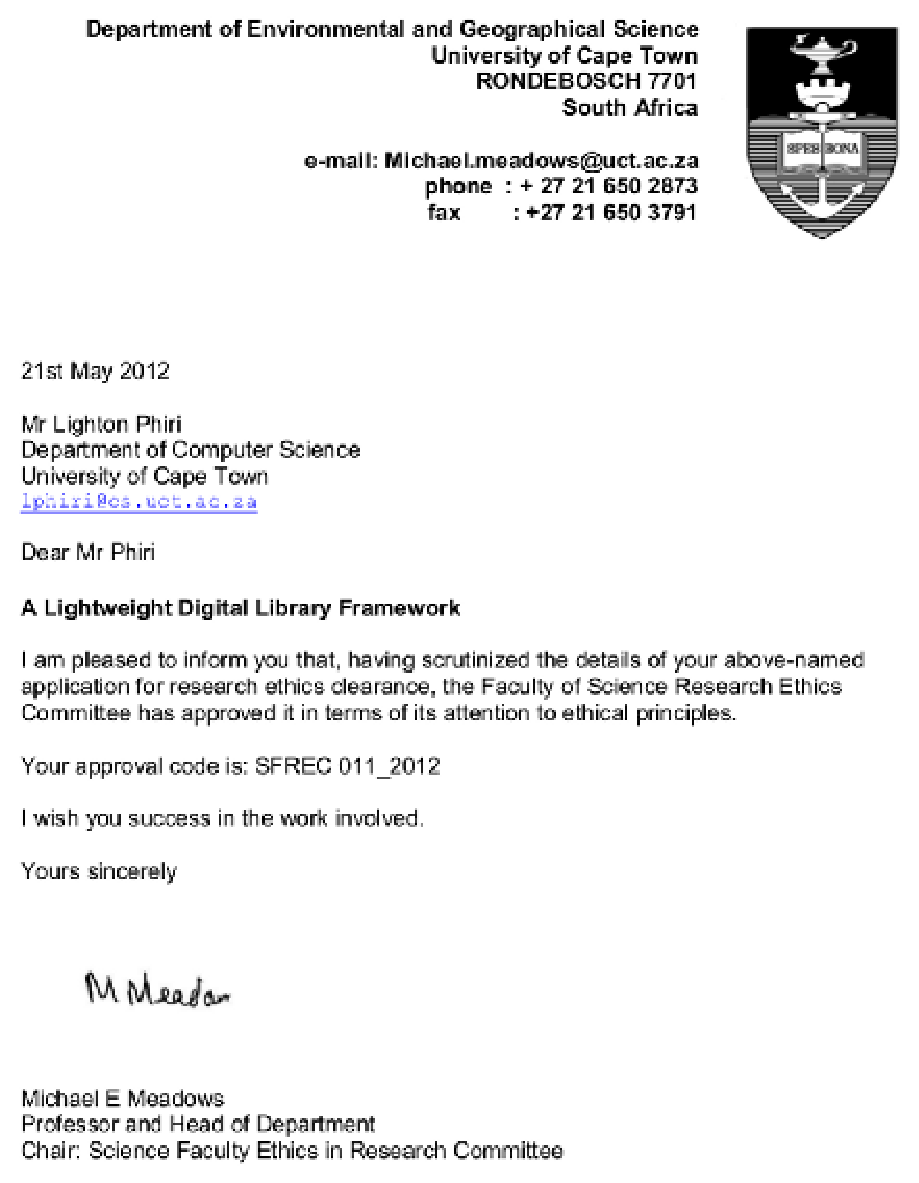
\includegraphics[width=0.95\textwidth]{appendicies/figures/ethics-clearance-faculty.eps}
 }
 \caption[Screenshot of faculty research ethical clearance]{Screenshot of faculty research ethical clearance}
 \label{ch:appendex-b:ethics-clearance:faculty-clearance}
\end{figure}

\begin{figure}
 \centering
 \framebox[\textwidth]{%
 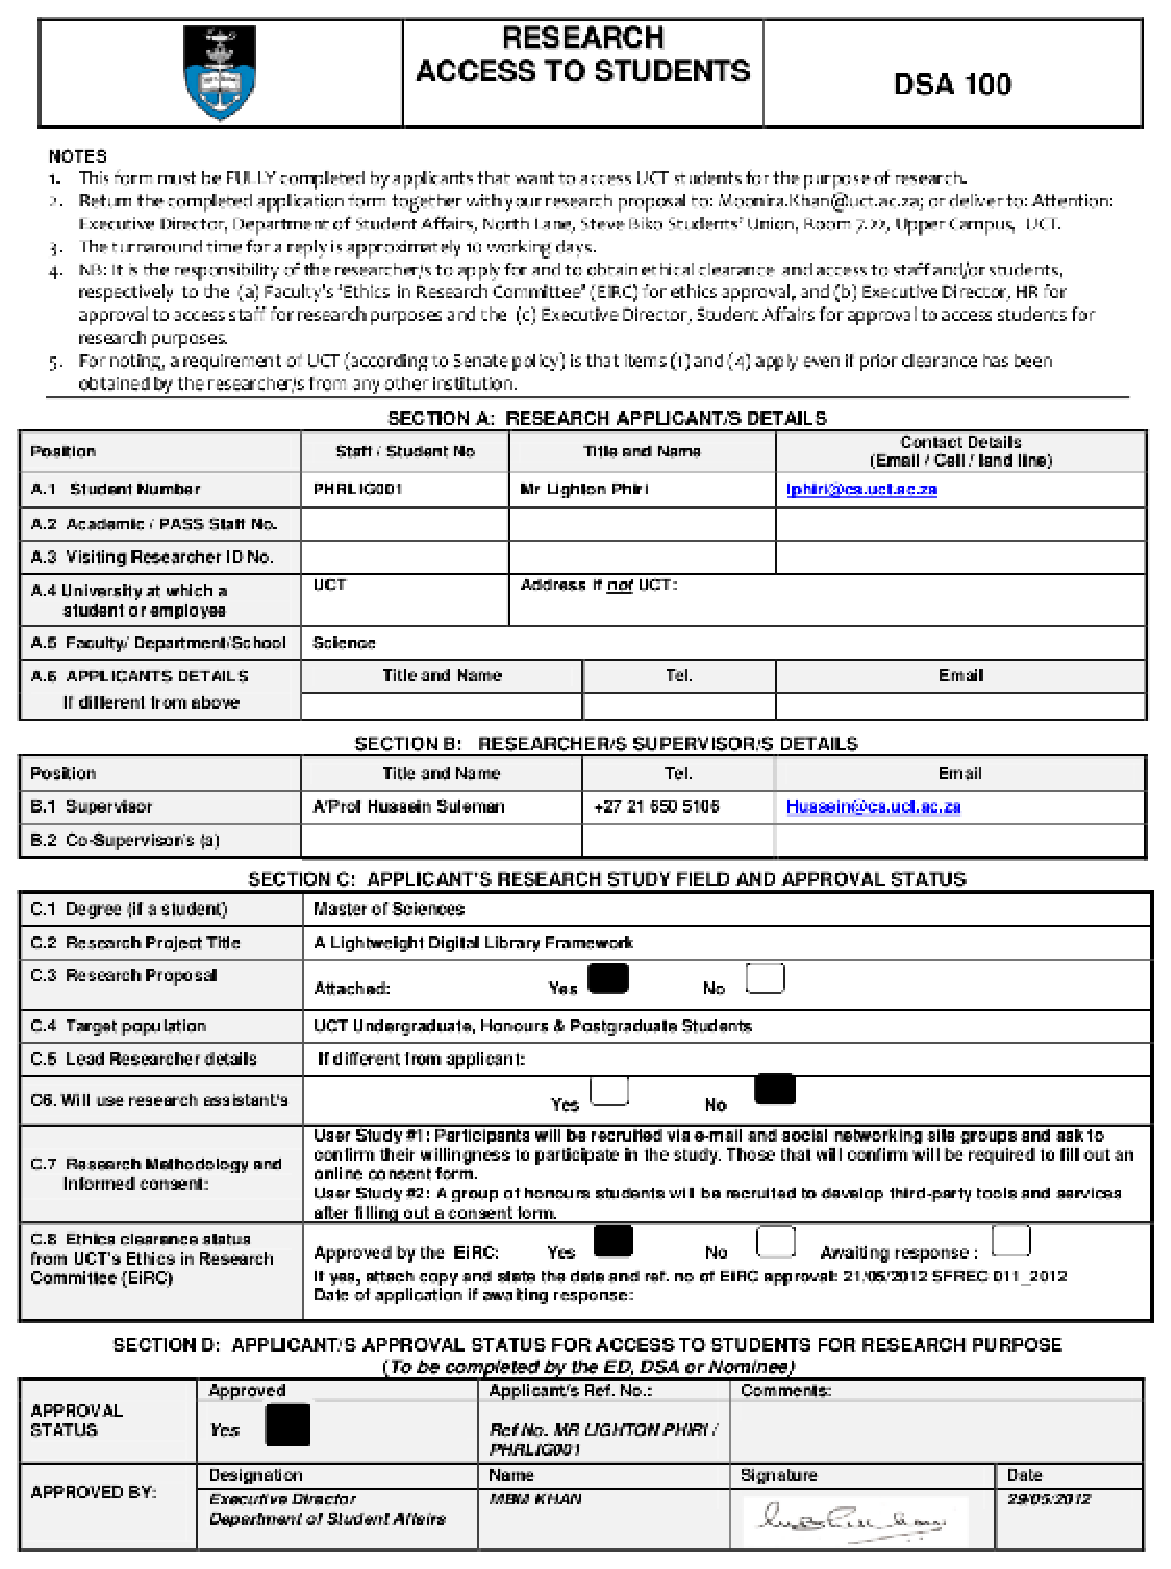
\includegraphics[width=0.95\textwidth]{appendicies/figures/ethics-clearance-access.eps}
 }
 \caption[Screenshot of student access ethical clearance]{Screenshot of student access ethical clearance}
 \label{ch:appendex-b:ethics-clearance:acess-clearance}
\end{figure}

%%%%%\chapter[Developer survey]{Developer survey\label{ch:appendex-c:developer-survey}}
\section{Survey design \label{ch:appendex-b:developer-survey:questionnaire-design}}

This appendix section provides auxiliary information related to the developer survey described in Section~\ref{sec:evaluation:developer-survey}. Figure~\ref{appendix:appendicies:developer-survey:WWW-survey-research-link} is a screenshot of the email sent to the target population inviting them to participate in the survey, Figure~\ref{appendix:appendicies:developer-survey:developer-survey-questionnaire1} is a screenshot of the \gls{www} practical programming assignment assigned to the target population, and Figures~\ref{appendix:appendicies:developer-suvery-one-page-001},~\ref{appendix:appendicies:developer-suvery-one-page-002},~\ref{appendix:appendicies:developer-suvery-one-page-003},~\ref{appendix:appendicies:developer-suvery-one-page-004} and~\ref{appendix:appendicies:developer-suvery-one-page-005} are screenshots of the post-assignment online questionnaire used by survey participants.

\begin{figure}
 \centering
 \framebox[\textwidth]{%
 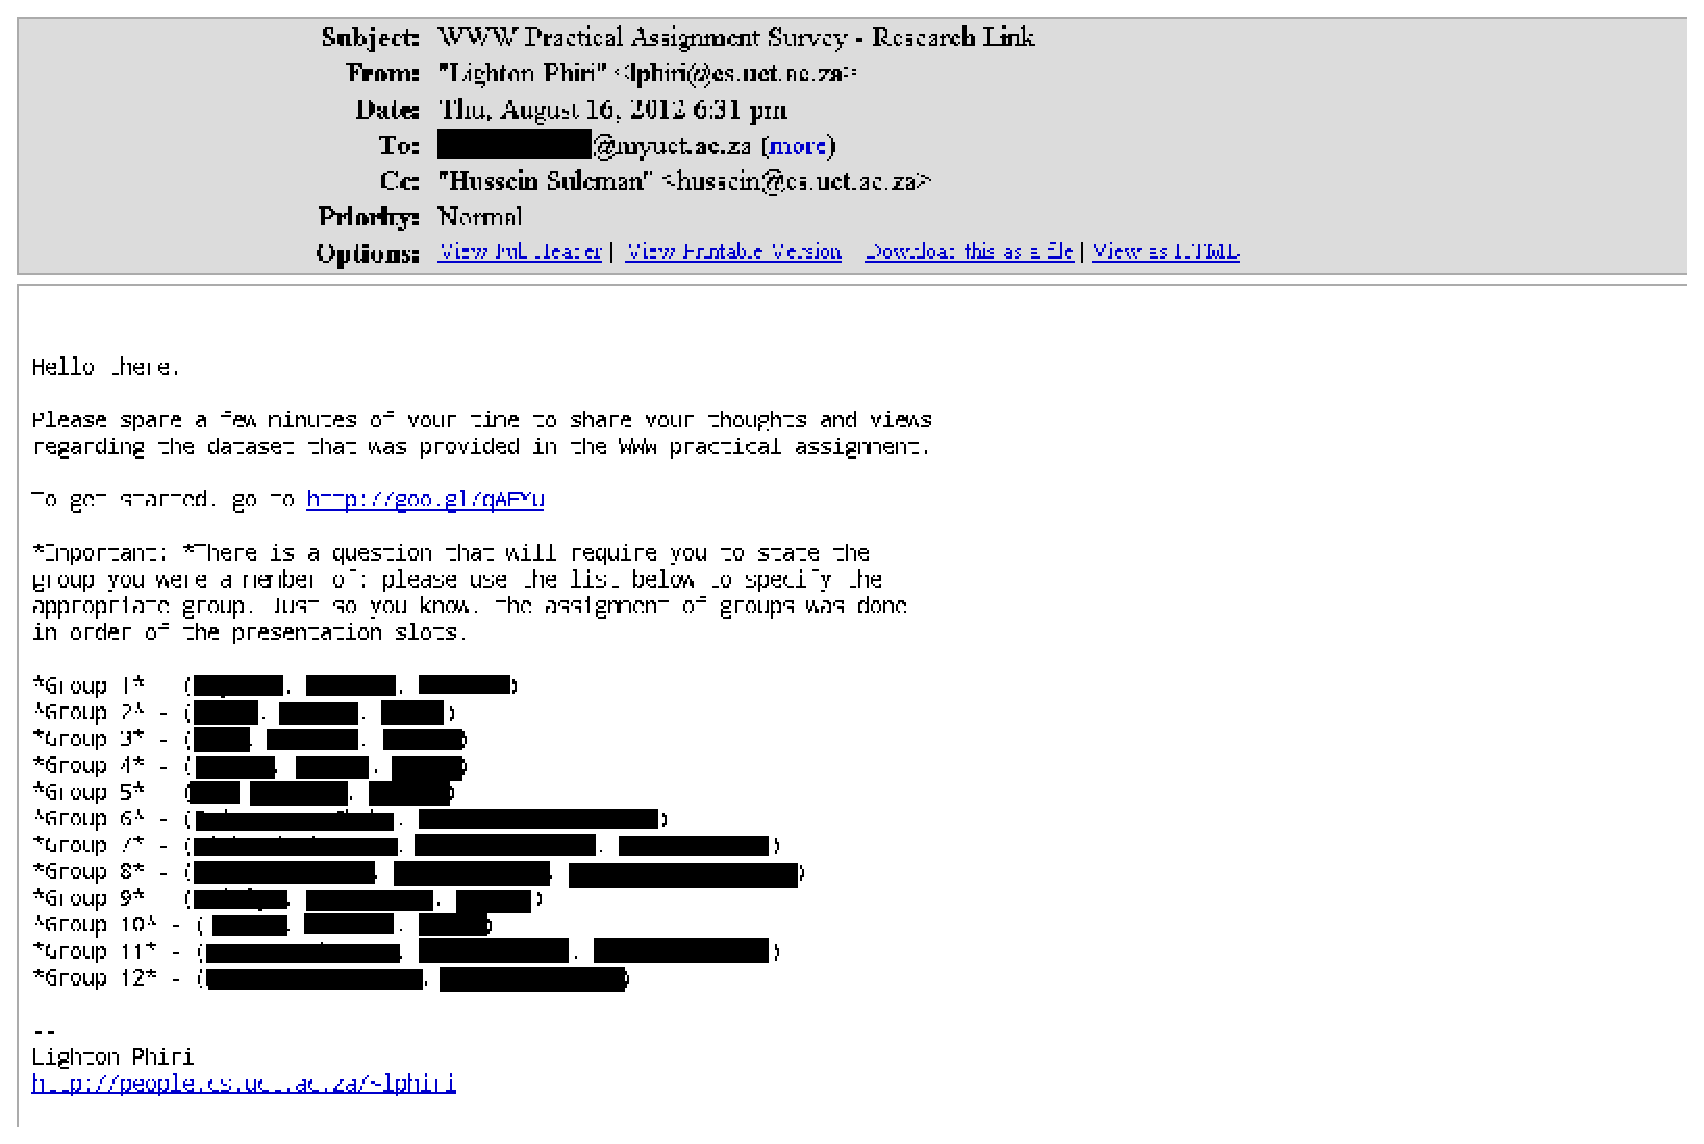
\includegraphics[width=0.95\textwidth]{appendicies/figures/WWW-survey-research-link-masked.eps}
 }
 \caption[Screenshot showing the survey participation email invitation]{Screenshot showing the WWW survey participation email invitation}
 \label{appendix:appendicies:developer-survey:WWW-survey-research-link}
\end{figure}

%\subsection{Section 1}
\begin{figure}
 \centering
 \framebox[\textwidth]{%
 \includegraphics[width=0.95\textwidth]{appendicies/figures/developer-assignment-question-screenshot.eps}
 }
 \caption[Screenshot showing the practical assignment question]{Screenshot showing the WWW practical programming assignment question}
 \label{appendix:appendicies:developer-survey:developer-survey-questionnaire1}
\end{figure}


% 
% subfigure and subfig packages deprecated
% http://en.wikibooks.org/wiki/LaTeX/Floats,_Figures_and_Captions#Subfloats

%\subsection{Section 1}
\begin{figure}
 \centering
 \subfloat[][]{%
 \framebox[\textwidth]{%
 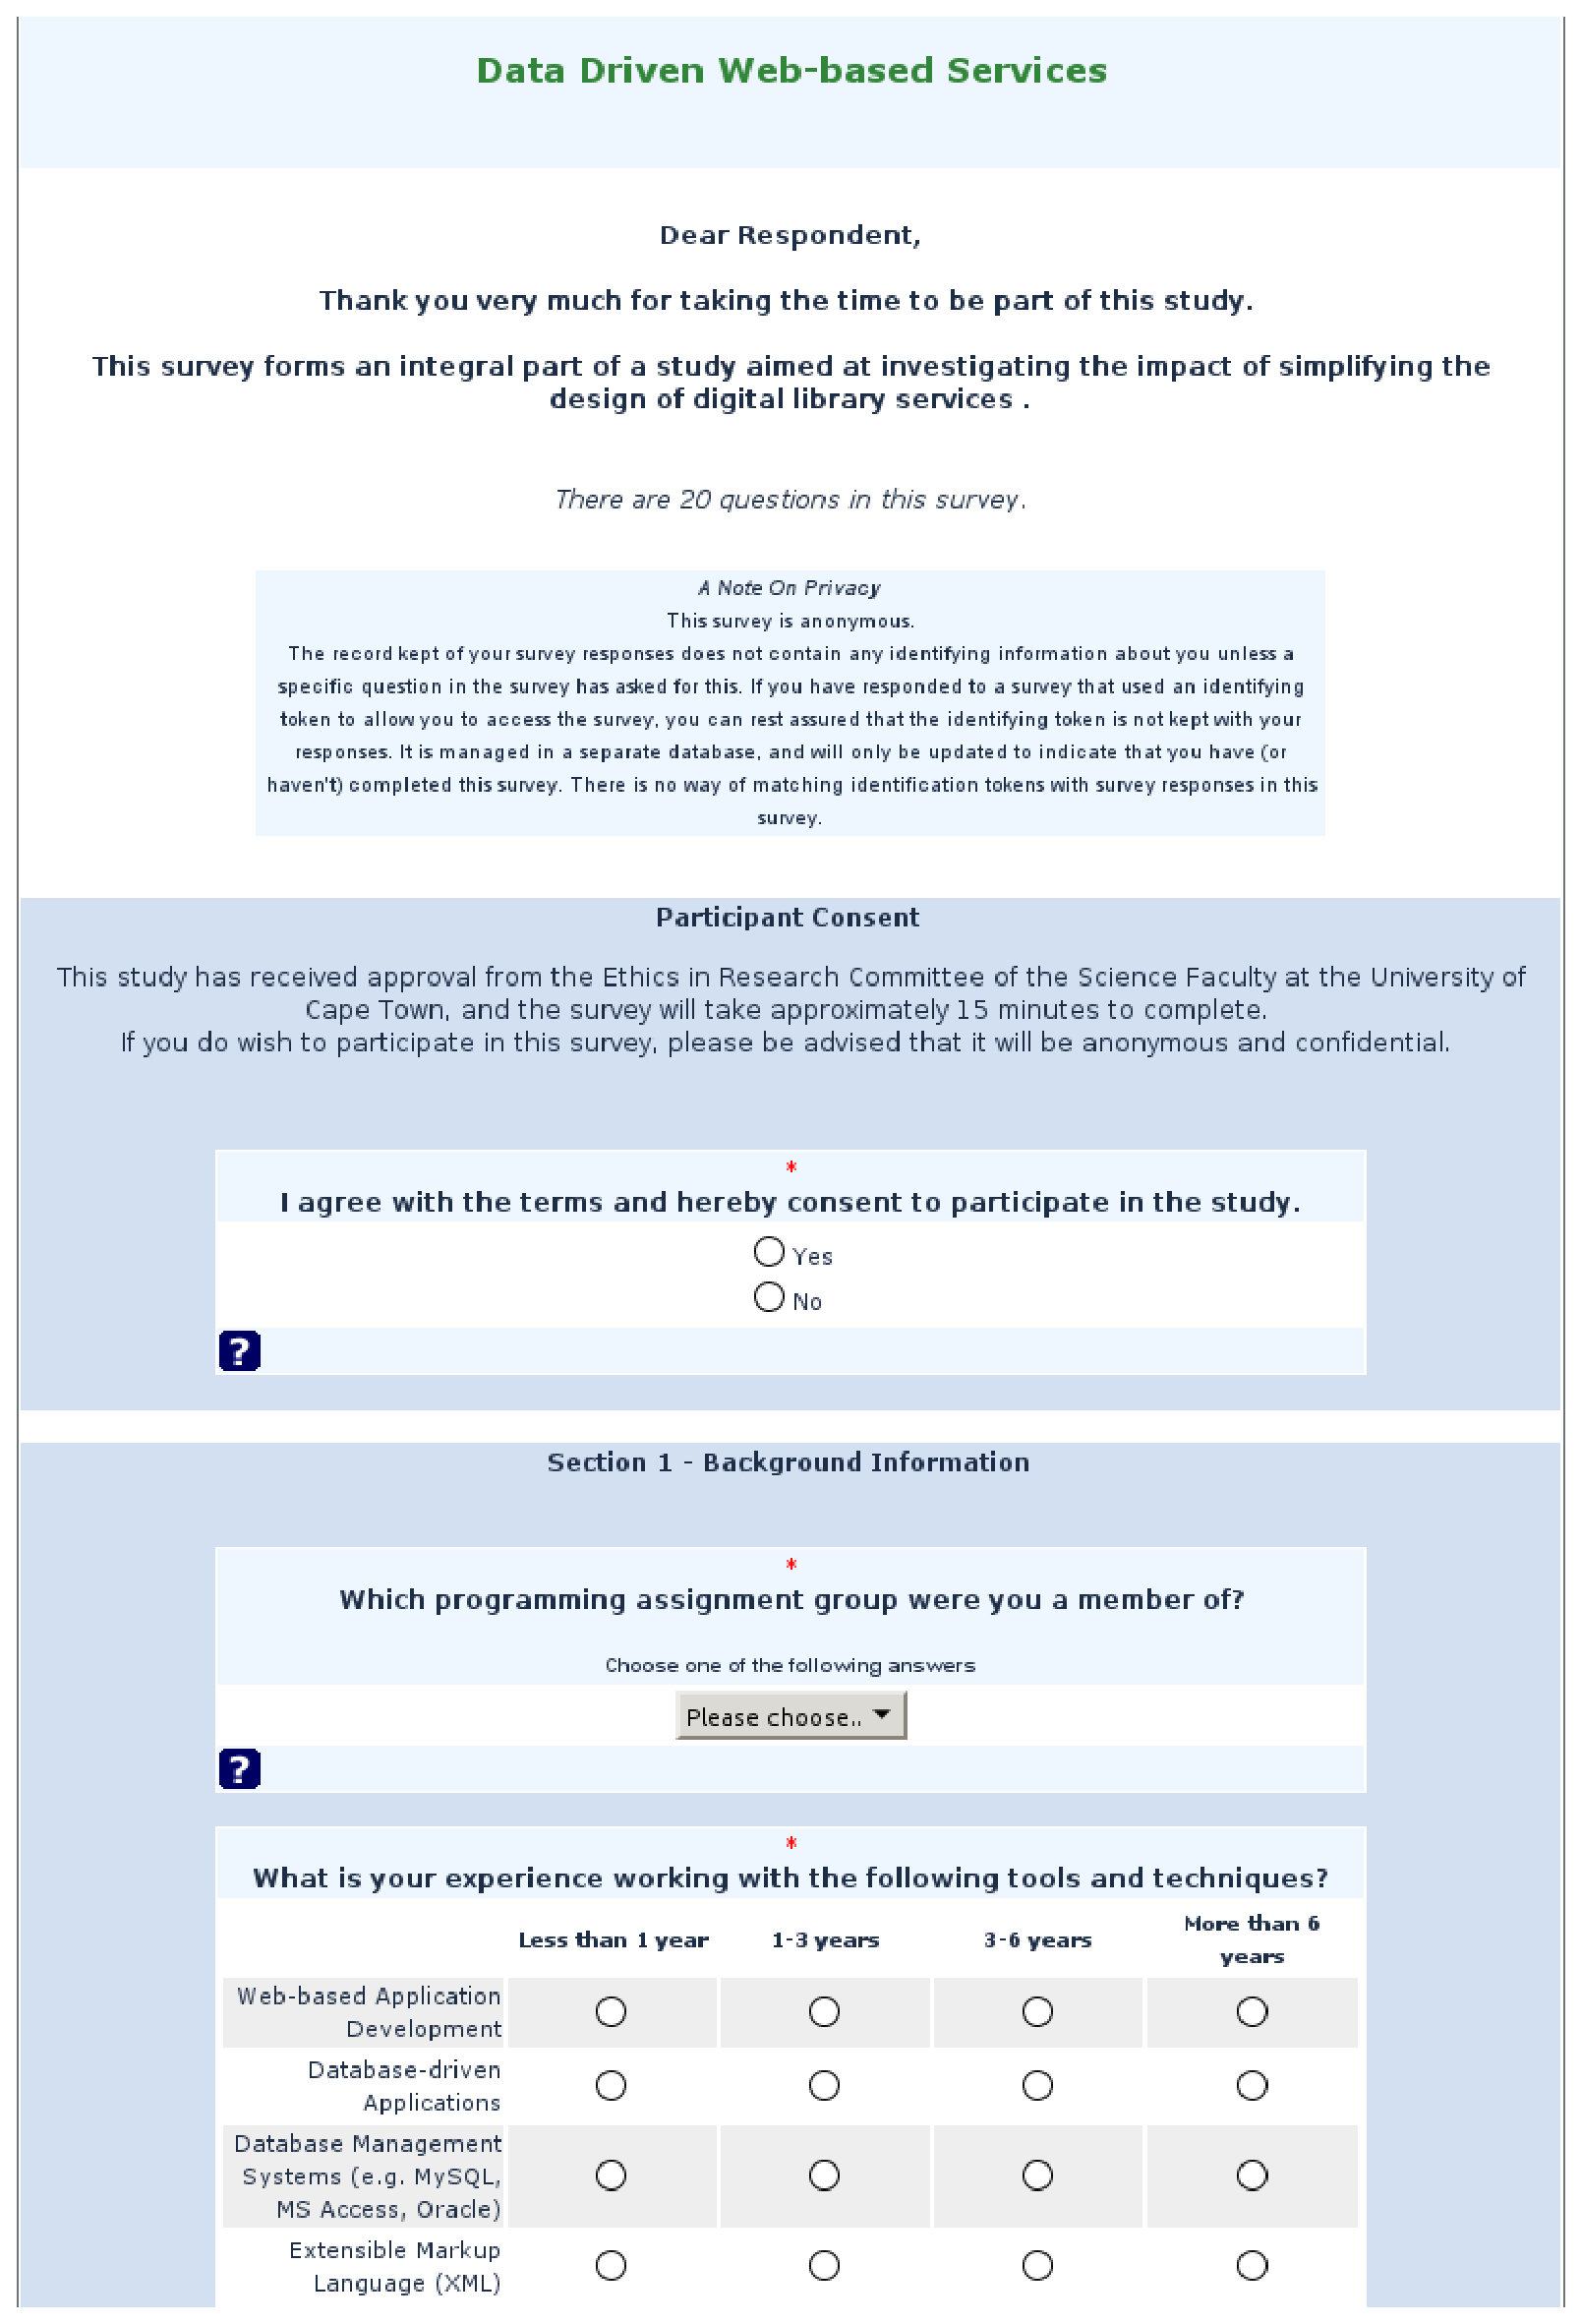
\includegraphics[width=0.95\textwidth]{appendicies/figures/developer-suvery-one-page-001.eps}
 }
 }
 \caption[Screenshot showing the online questionnaire (page 1 of 5)]{Screenshot showing the online LimeSurvey questionnaire (page 1 of 5)}
 \label{appendix:appendicies:developer-suvery-one-page-001}
\end{figure}

%\subsection{Section 1}
\begin{figure}
\ContinuedFloat
 \centering
 \subfloat[][]{%
 \framebox[\textwidth]{%
 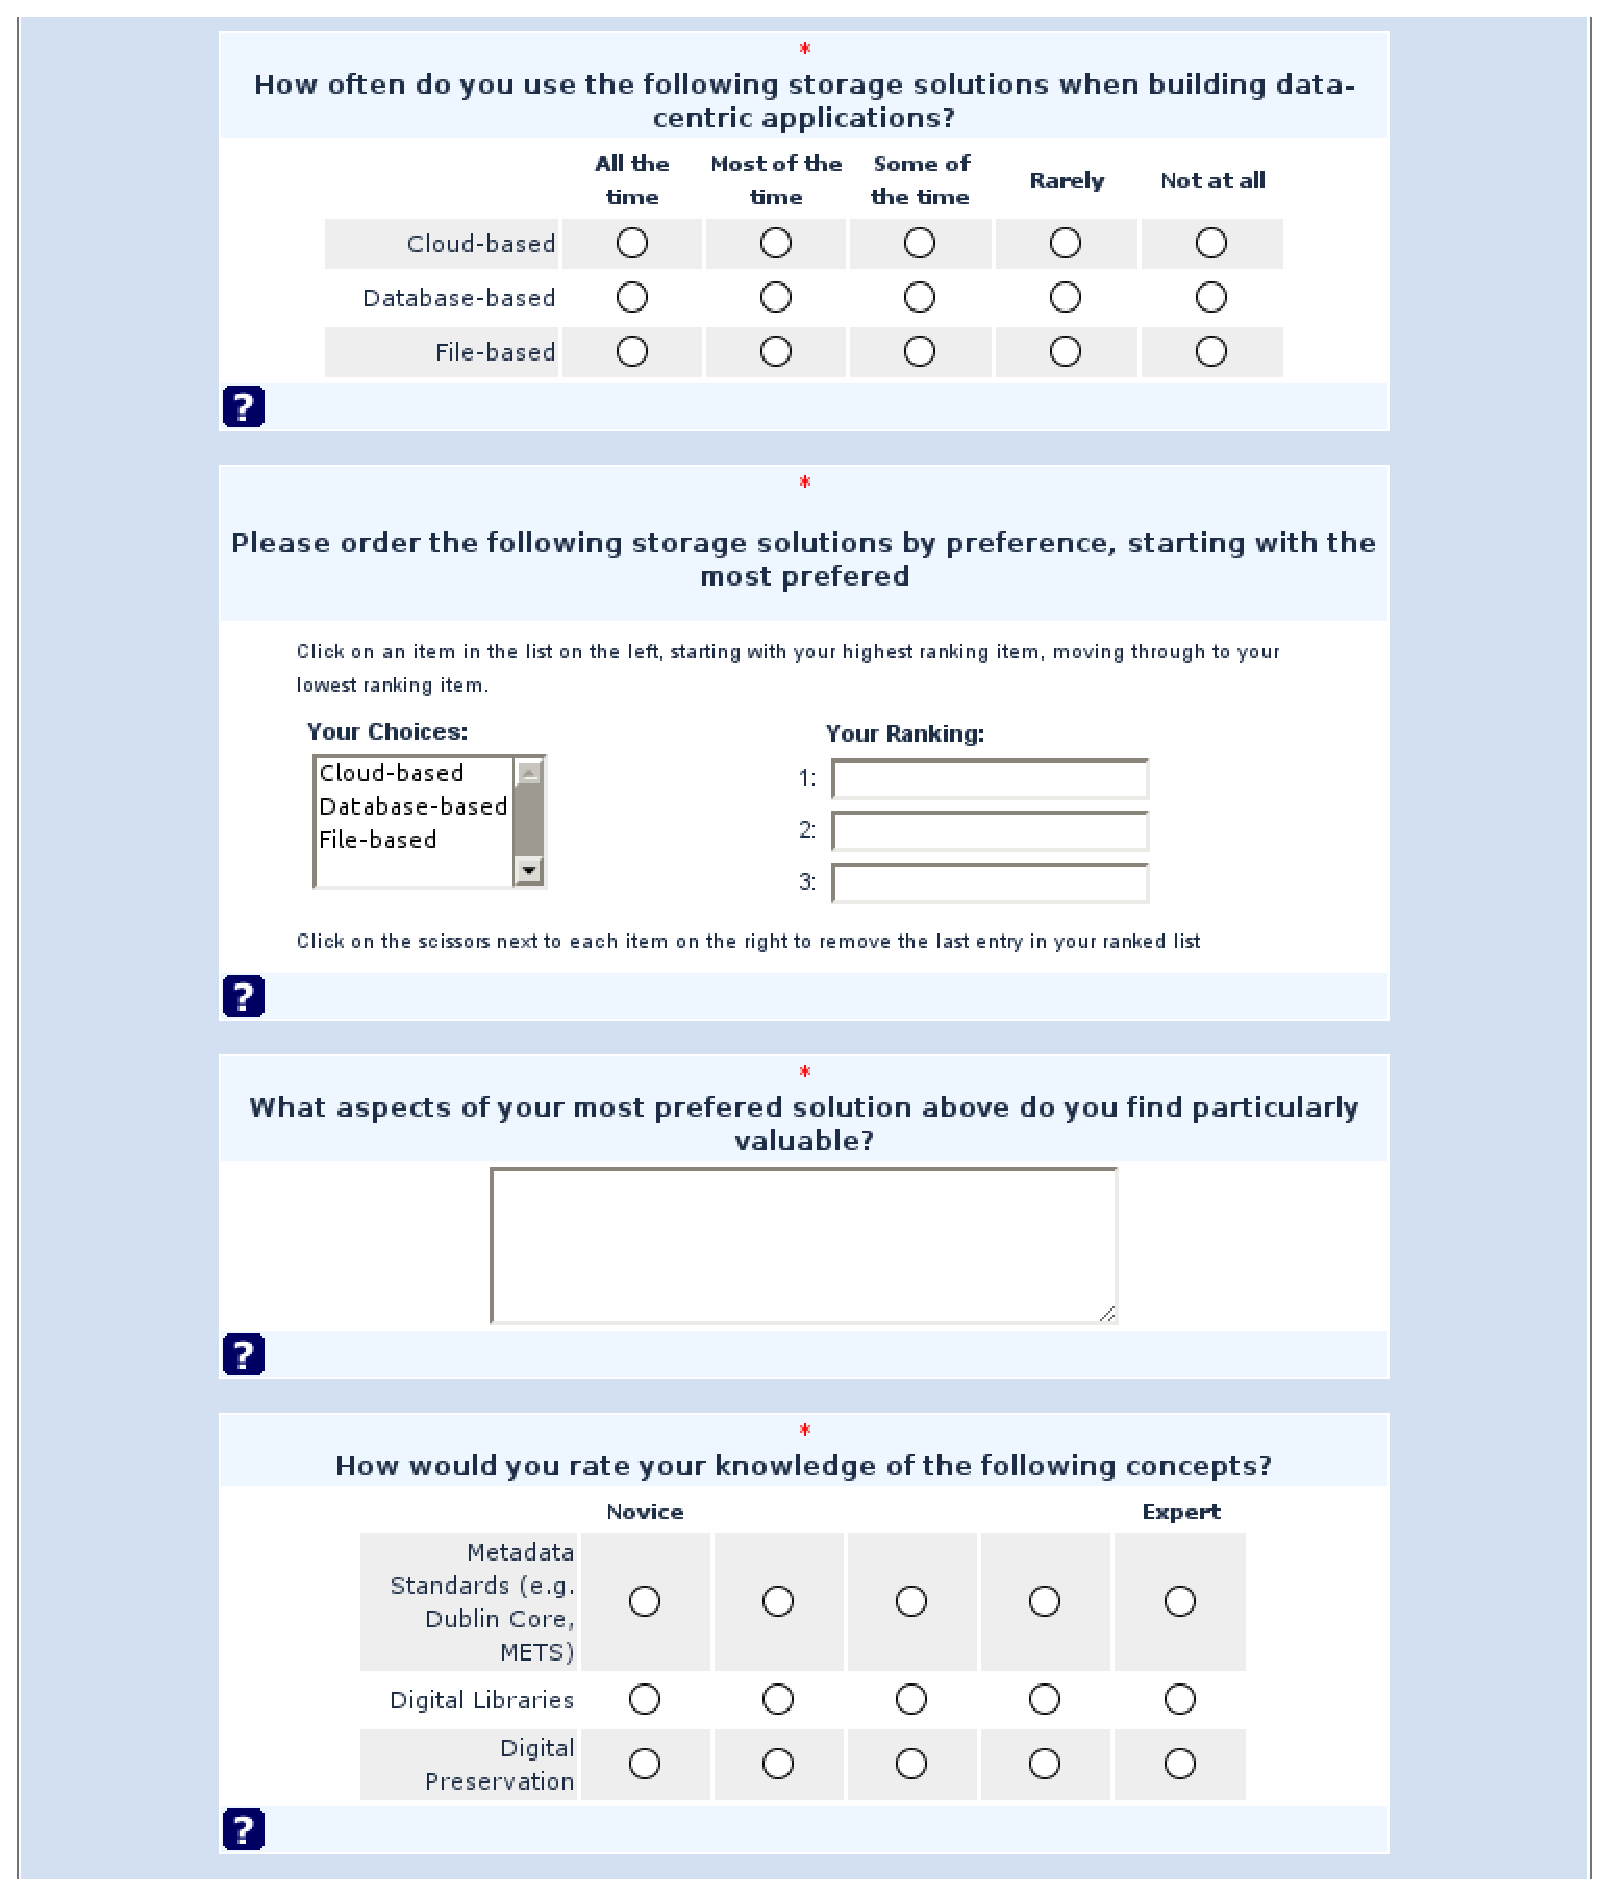
\includegraphics[width=0.95\textwidth]{appendicies/figures/developer-suvery-one-page-002.eps}
 }
 }
 \caption[Screenshot showing the online questionnaire (page 2 of 5)]{Screenshot showing the online LimeSurvey questionnaire (page 2 of 5)}
 \label{appendix:appendicies:developer-suvery-one-page-002}
\end{figure}


%\subsection{Section 1}
\begin{figure}
\ContinuedFloat
 \centering
 \subfloat[][]{%
 \framebox[\textwidth]{%
 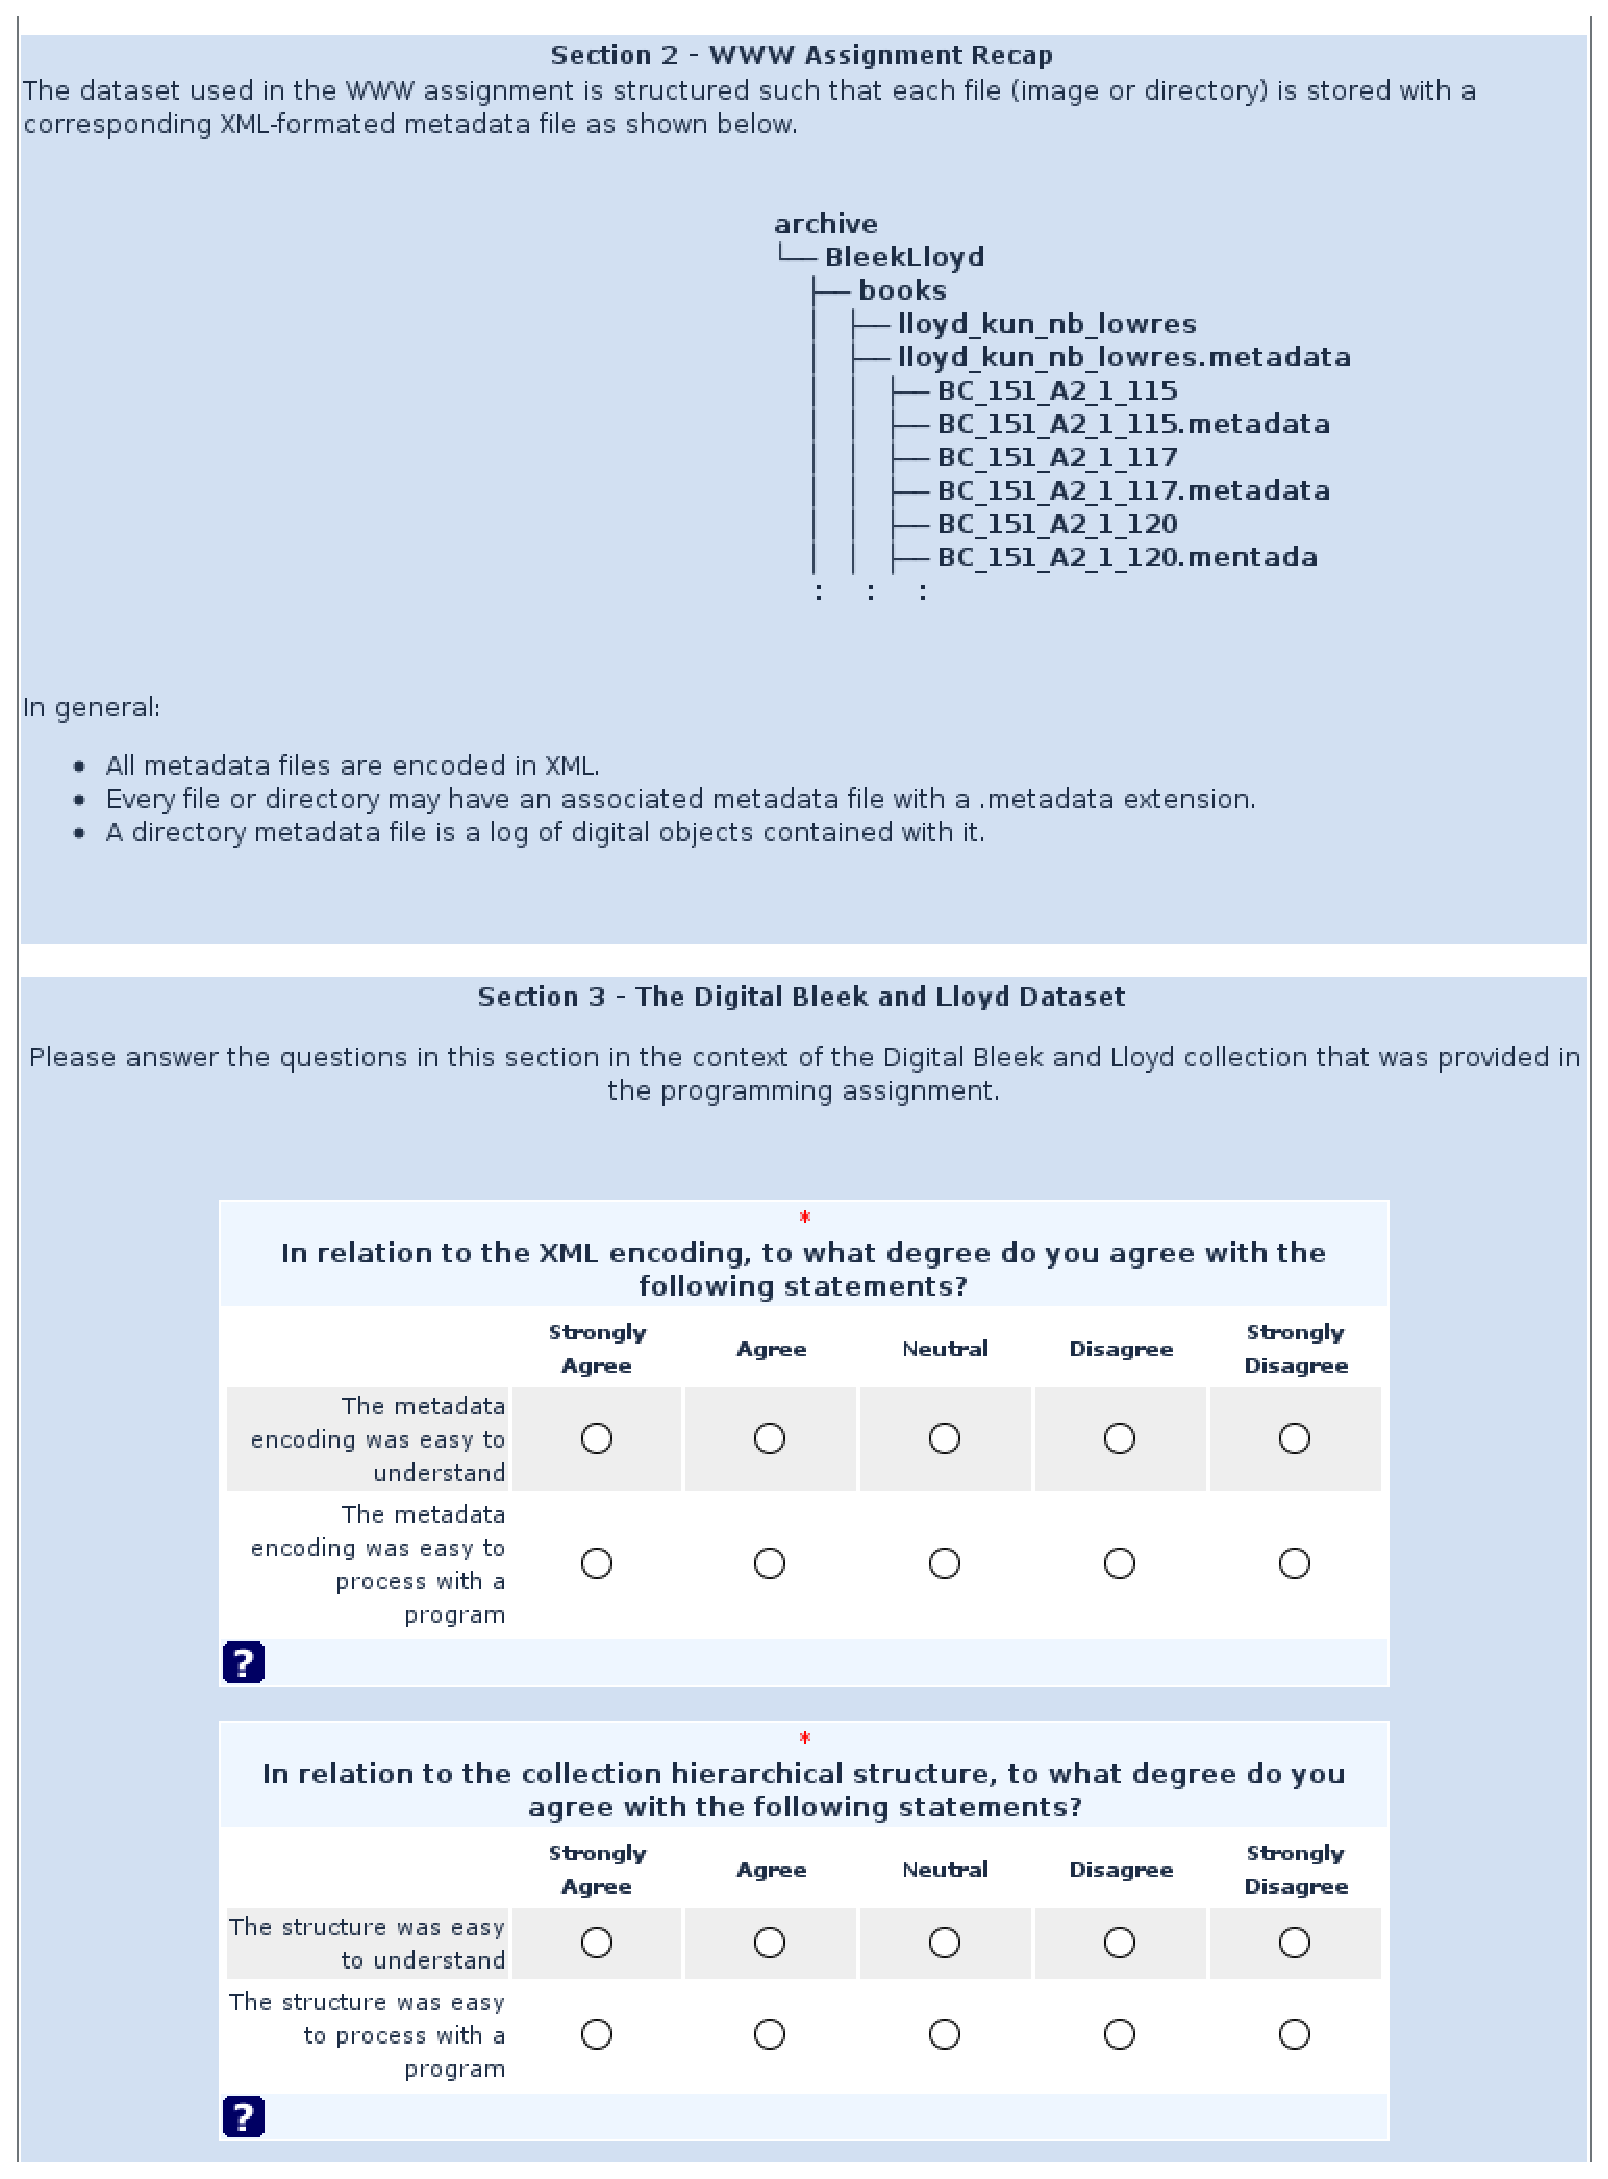
\includegraphics[width=0.95\textwidth]{appendicies/figures/developer-suvery-one-page-003.eps}
 }
 }
 \caption[Screenshot showing the online questionnaire (page 3 of 5)]{Screenshot showing the online LimeSurvey questionnaire (page 3 of 5)}
 \label{appendix:appendicies:developer-suvery-one-page-003}
\end{figure}


%\subsection{Section 1}
\begin{figure}
\ContinuedFloat
 \centering
 \subfloat[][]{%
 \framebox[\textwidth]{%
 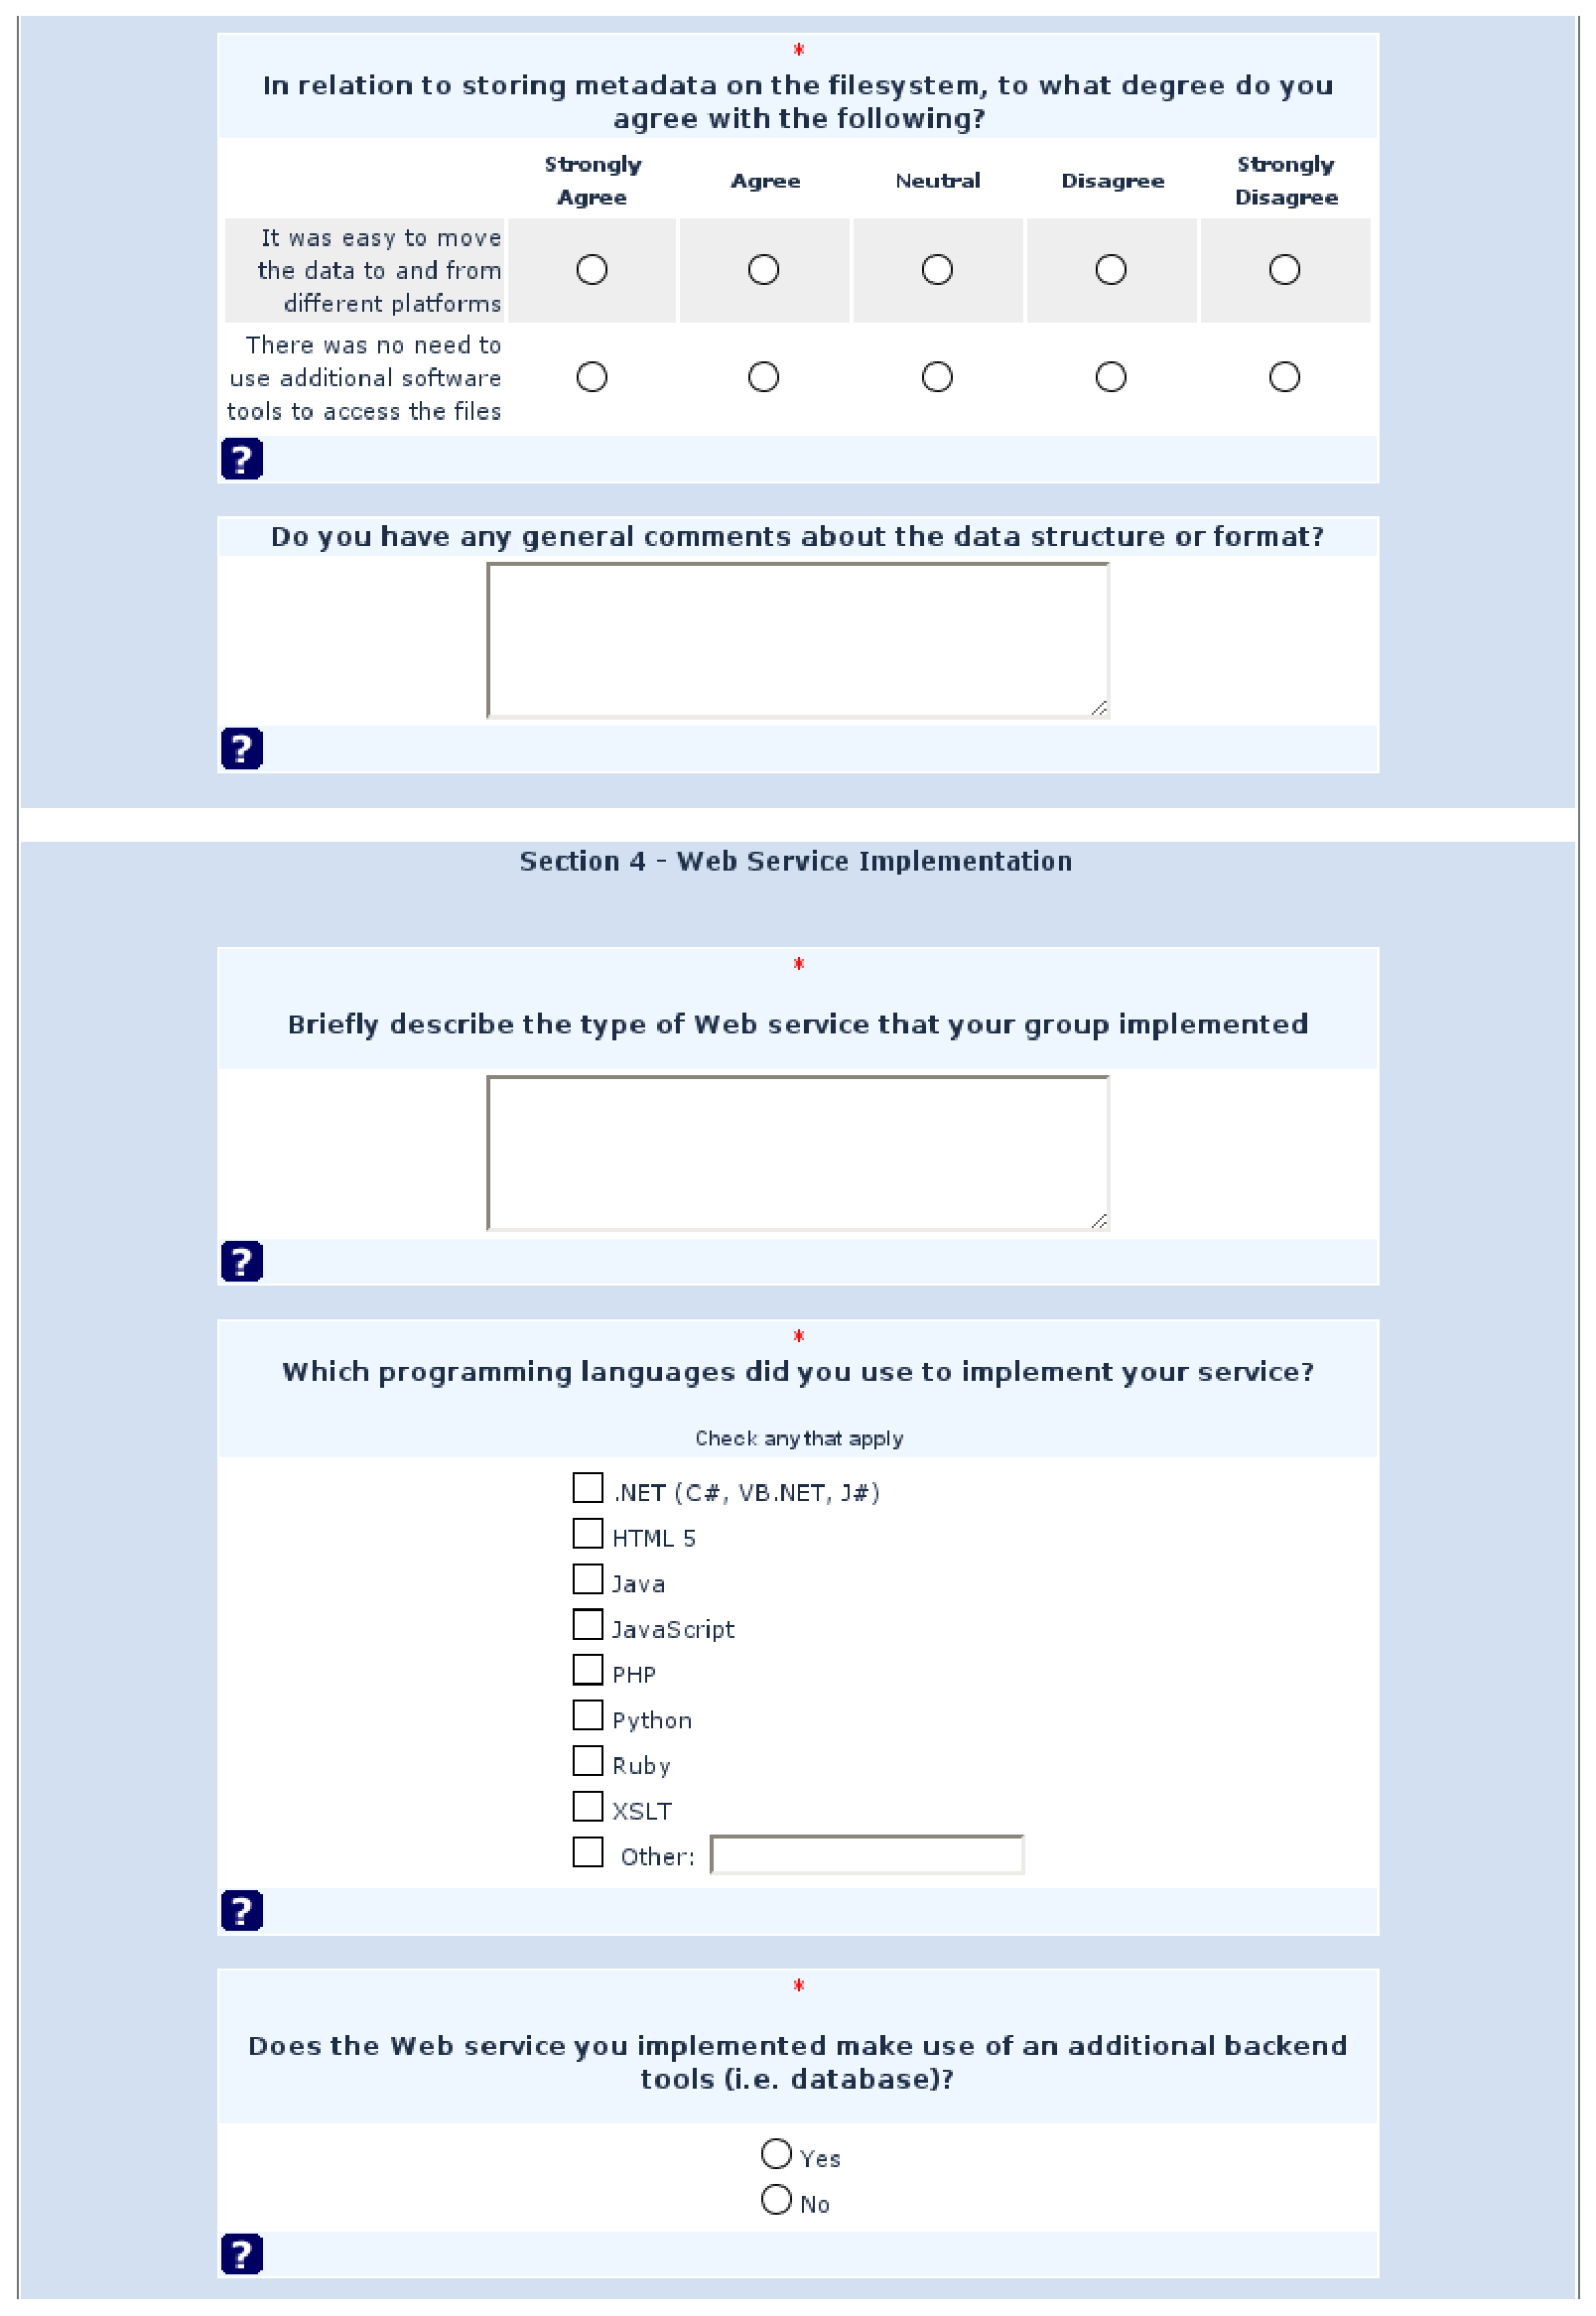
\includegraphics[width=0.95\textwidth]{appendicies/figures/developer-suvery-one-page-004.eps}
 }
 }
 \caption[Screenshot showing the online questionnaire (page 4 of 5)]{Screenshot showing the online LimeSurvey questionnaire (page 4 of 5)}
 \label{appendix:appendicies:developer-suvery-one-page-004}
\end{figure}


%\subsection{Section 1}
\begin{figure}
\ContinuedFloat
 \centering
 \subfloat[][]{%
 \framebox[\textwidth]{%
 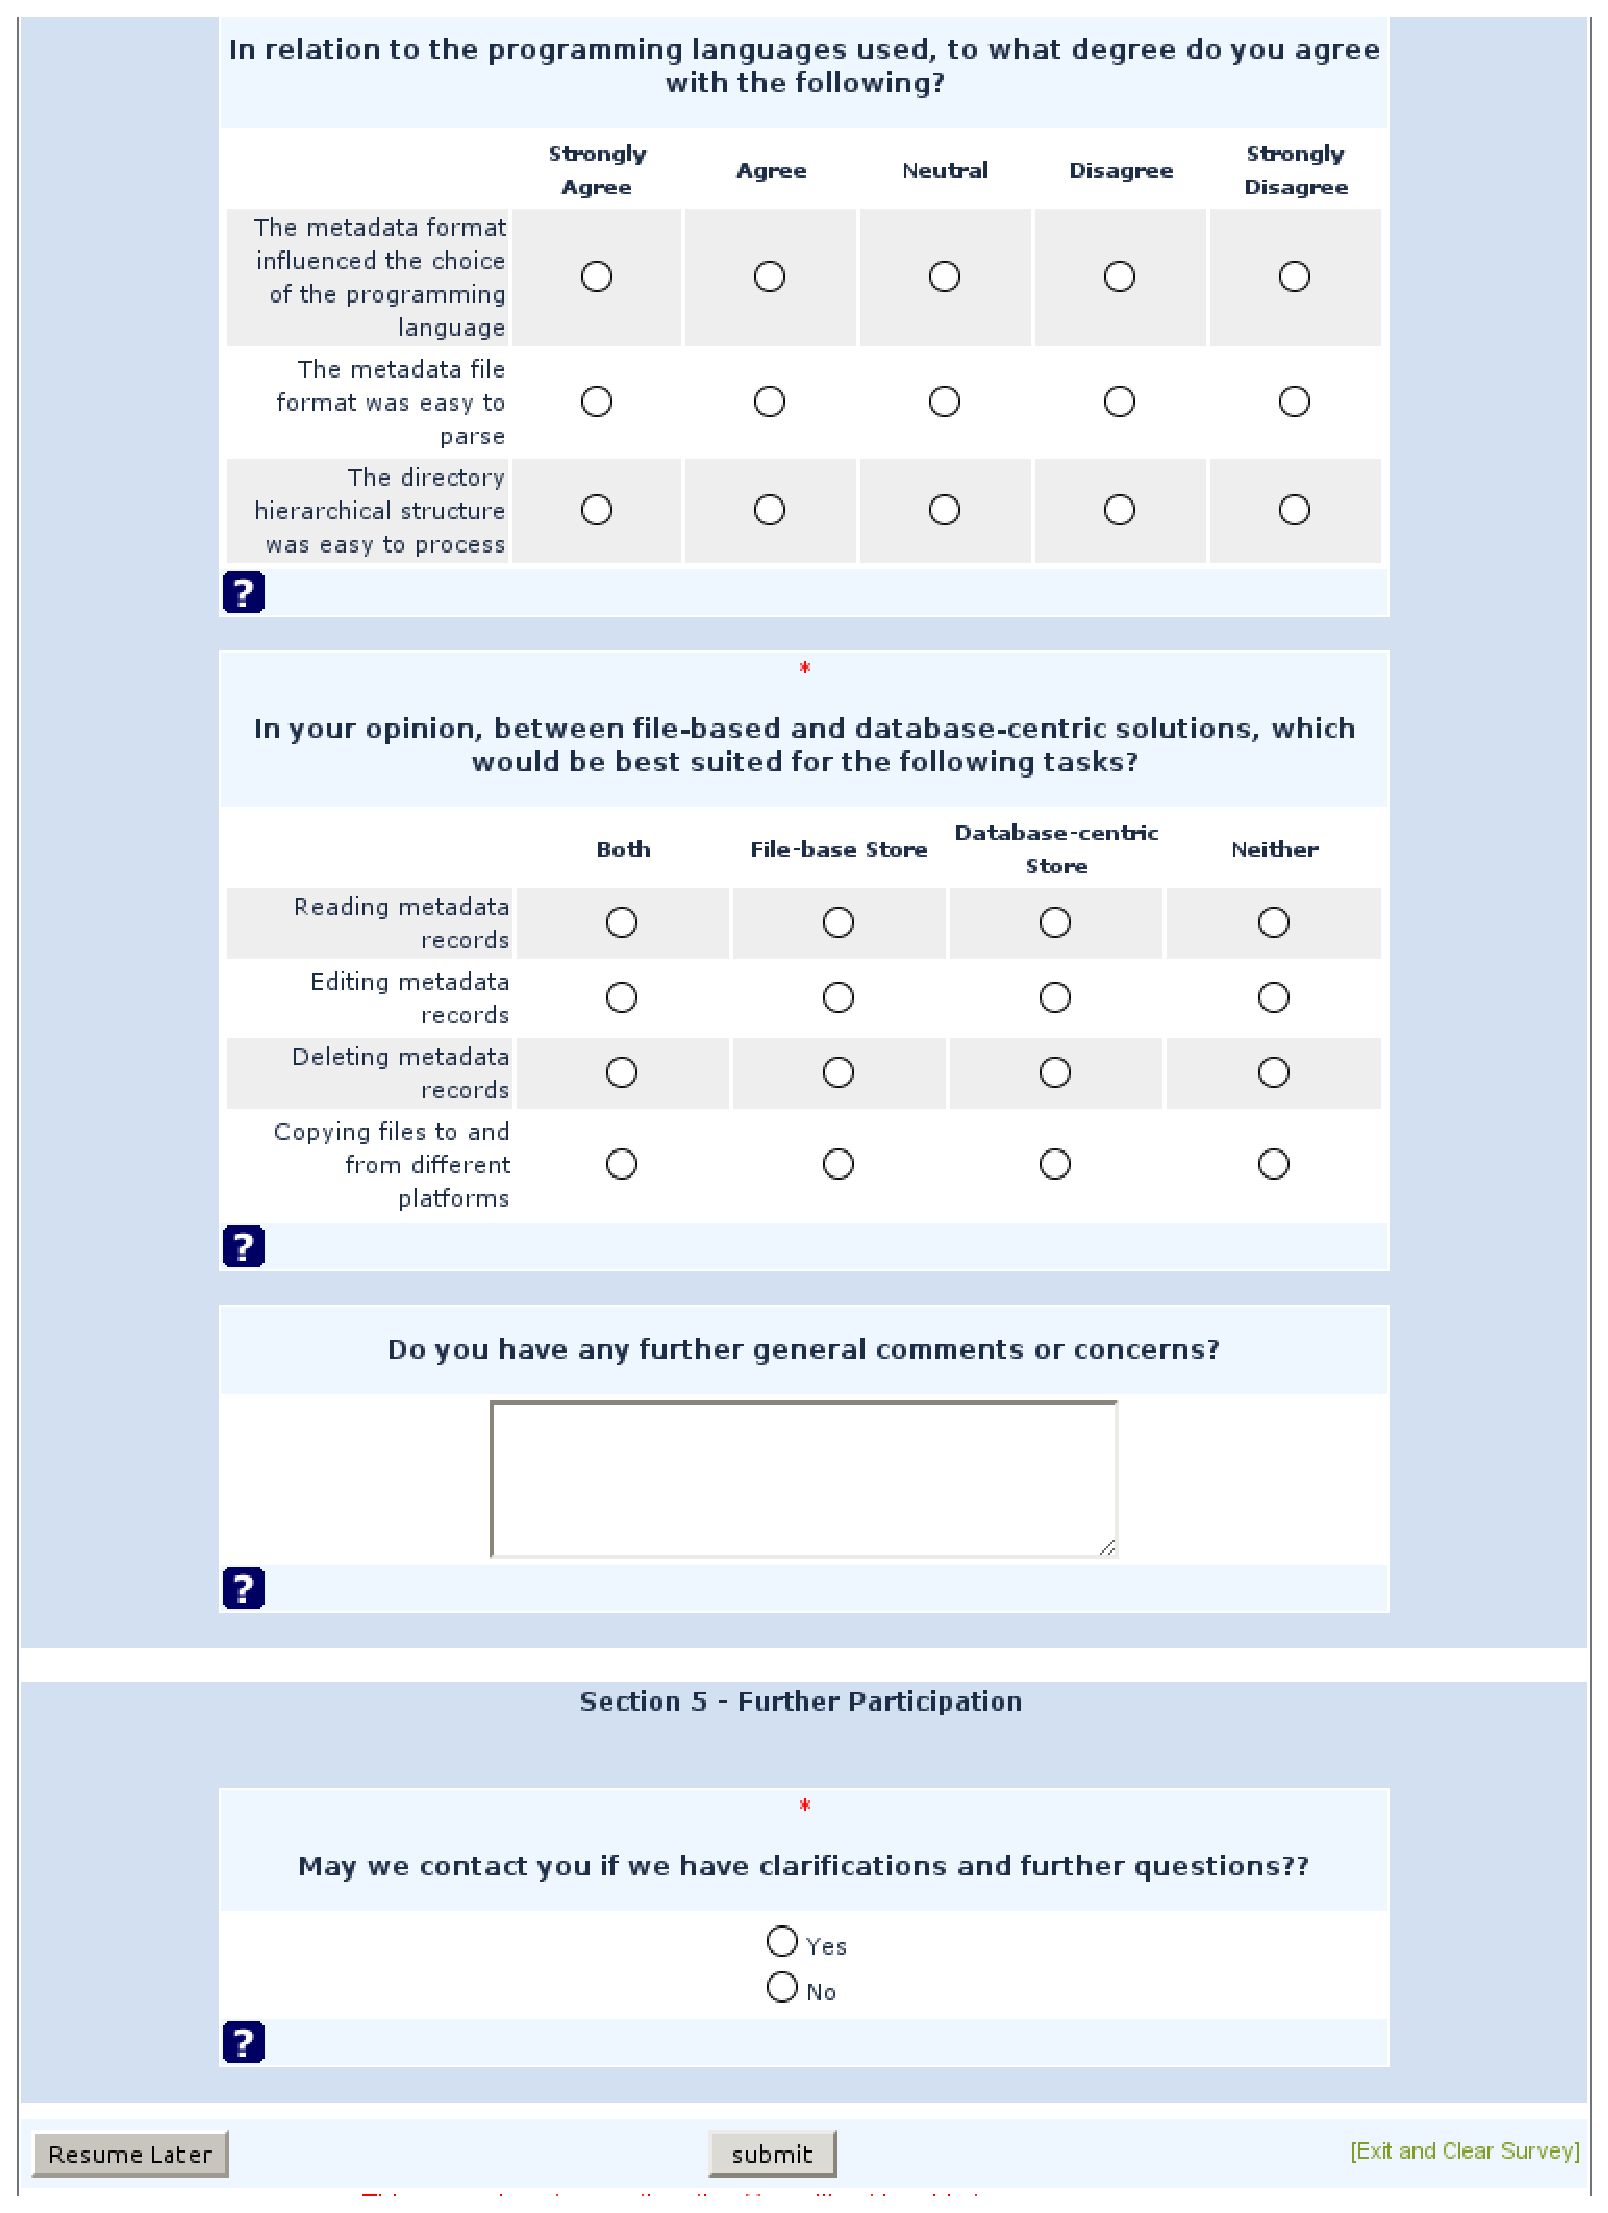
\includegraphics[width=0.95\textwidth]{appendicies/figures/developer-suvery-one-page-005.eps}
 }
 }
 \caption[Screenshot showing the online questionnaire (page 5 of 5)]{Screenshot showing the online LimeSurvey questionnaire (page 5 of 5)}
 \label{appendix:appendicies:developer-suvery-one-page-005}
\end{figure}


\begin{comment}
\begin{figure}
%\subsection{Section 1}
\begin{subfigure}[b]{\textwidth}
 \centering
 \framebox[\textwidth]{%
 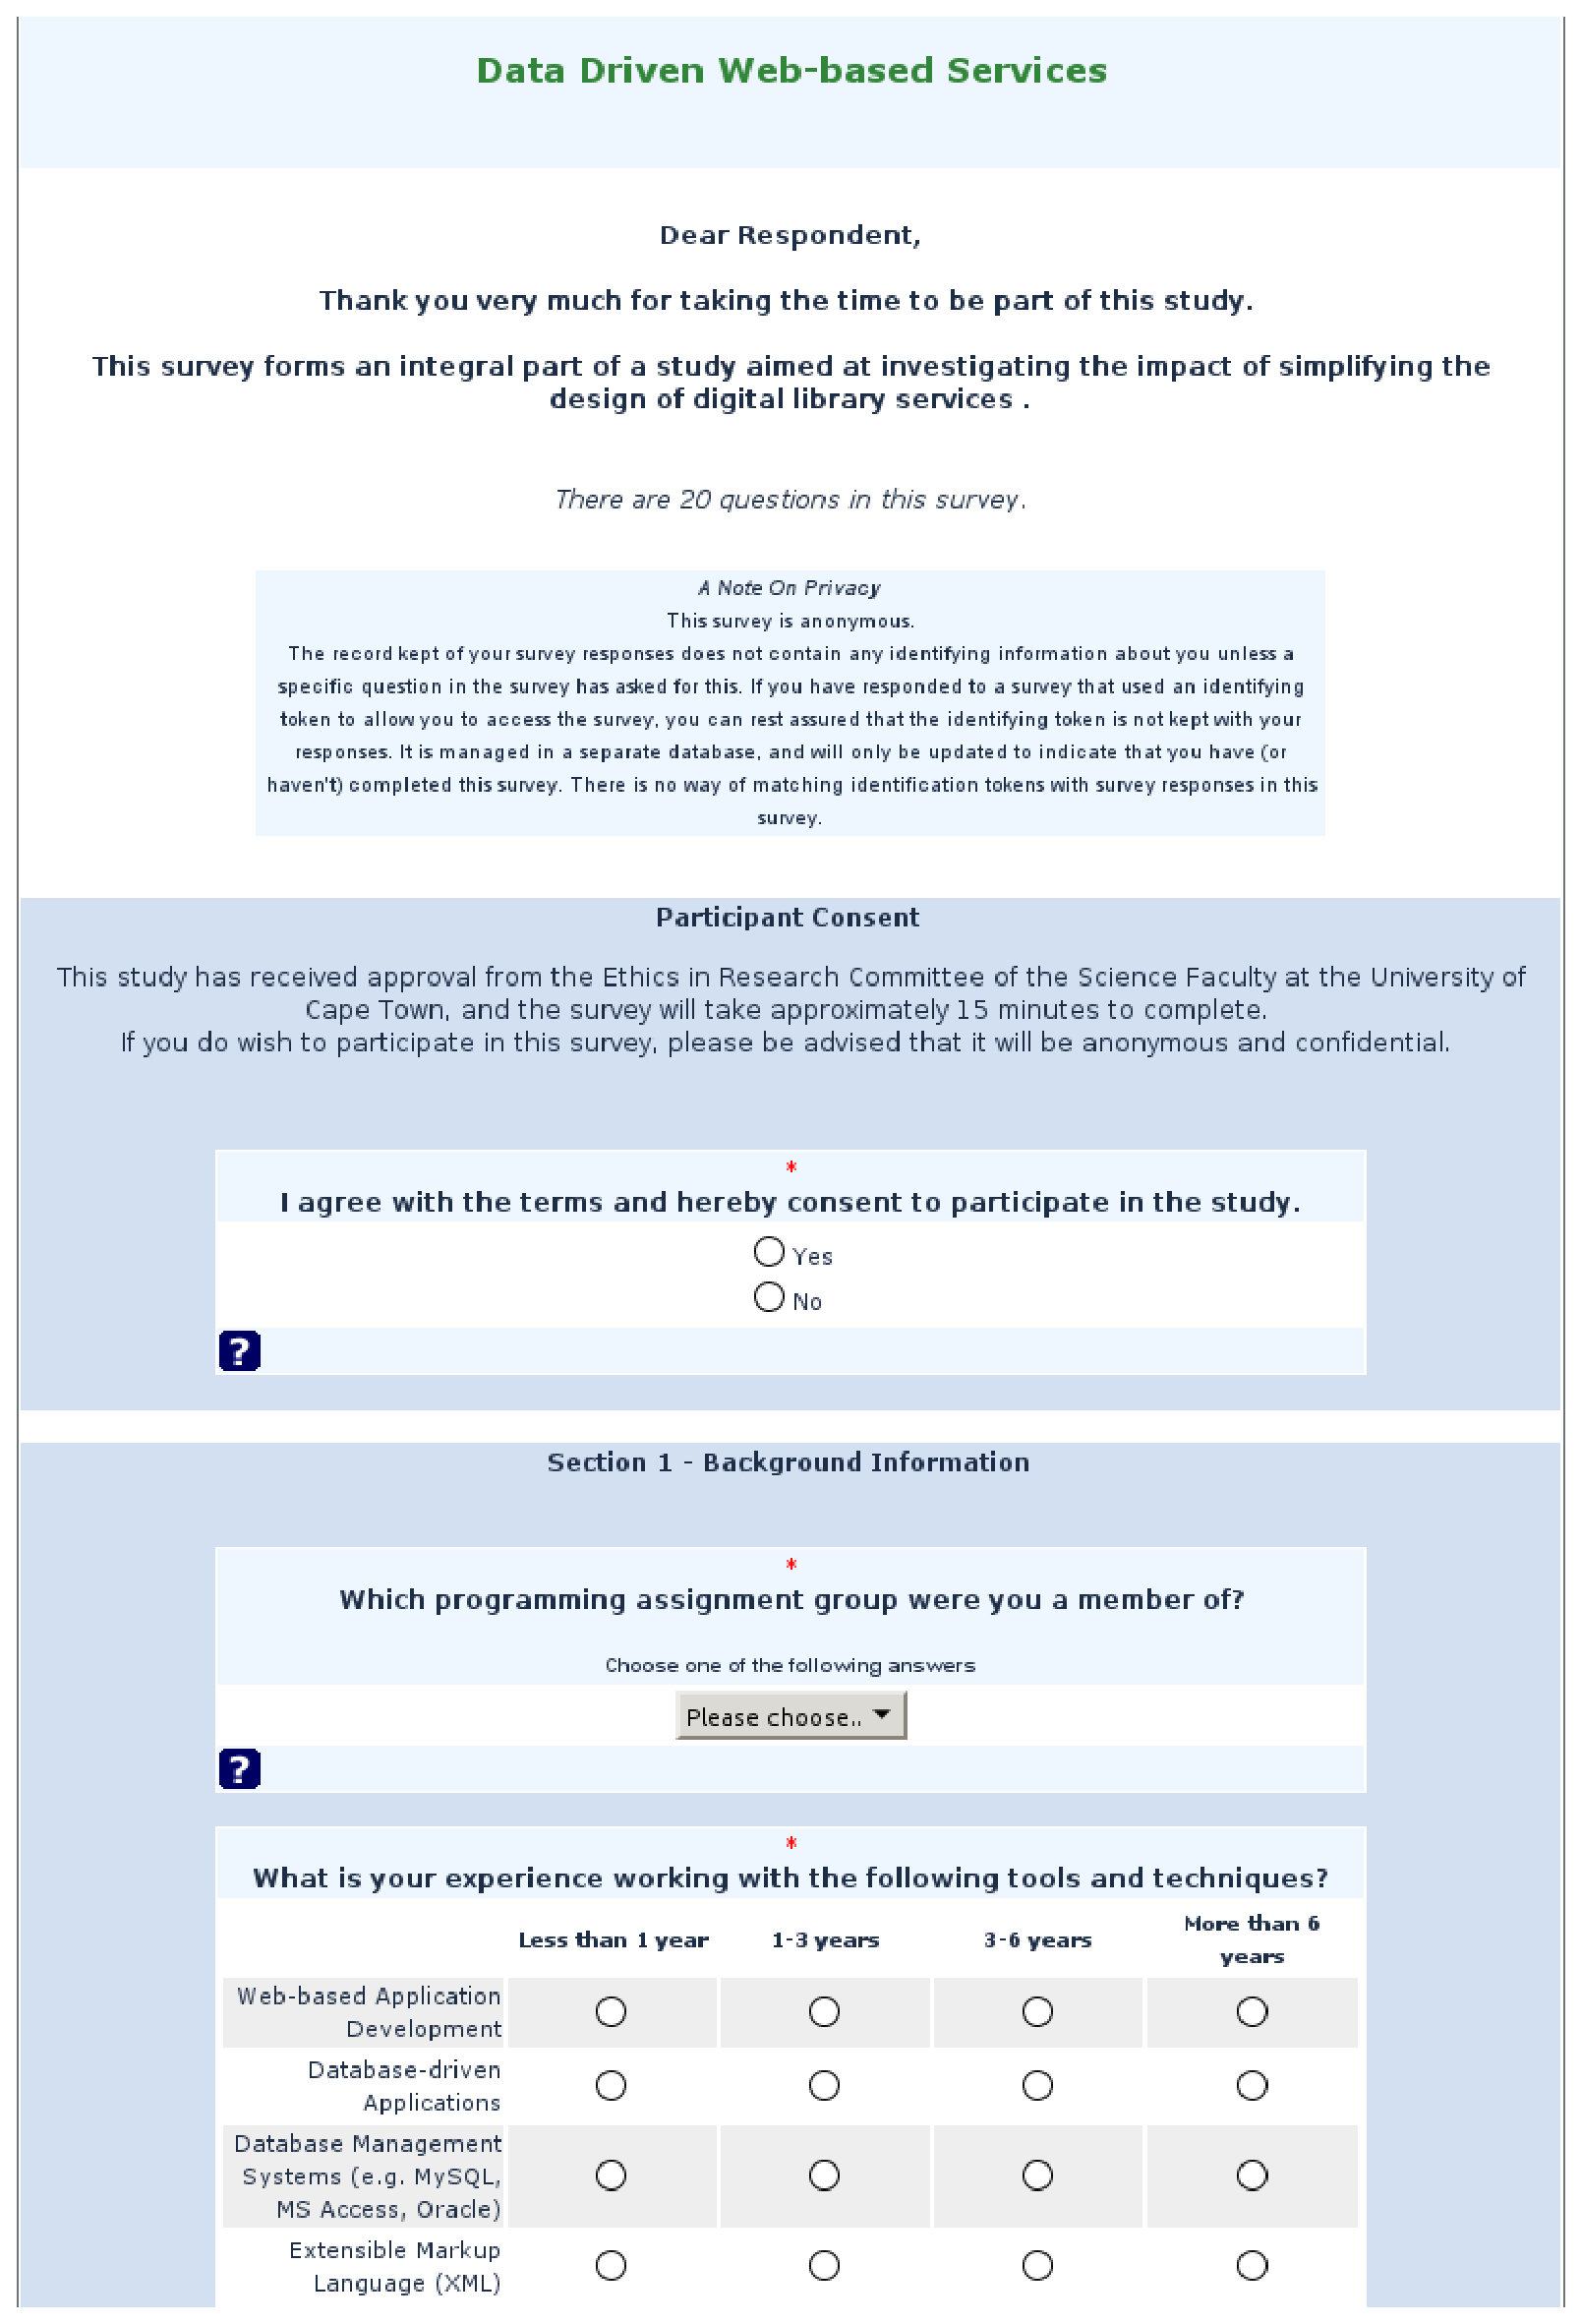
\includegraphics[width=0.95\textwidth]{appendicies/figures/developer-suvery-one-page-001.eps}
 }
 \caption[Screenshot of the online questionnaire (page 1 of 5)]{Screenshot of the online LimeSurvey questionnaire (page 1 of 5)}
 \label{appendix:appendicies:developer-suvery-one-page-001}
\end{subfigure}

\newpage

%\subsection{Section 1}
\begin{subfigure}[h]{\textwidth}
 \ContinuedFloat
 \centering
 %\subfloat[][]
 \framebox[\textwidth]{%
 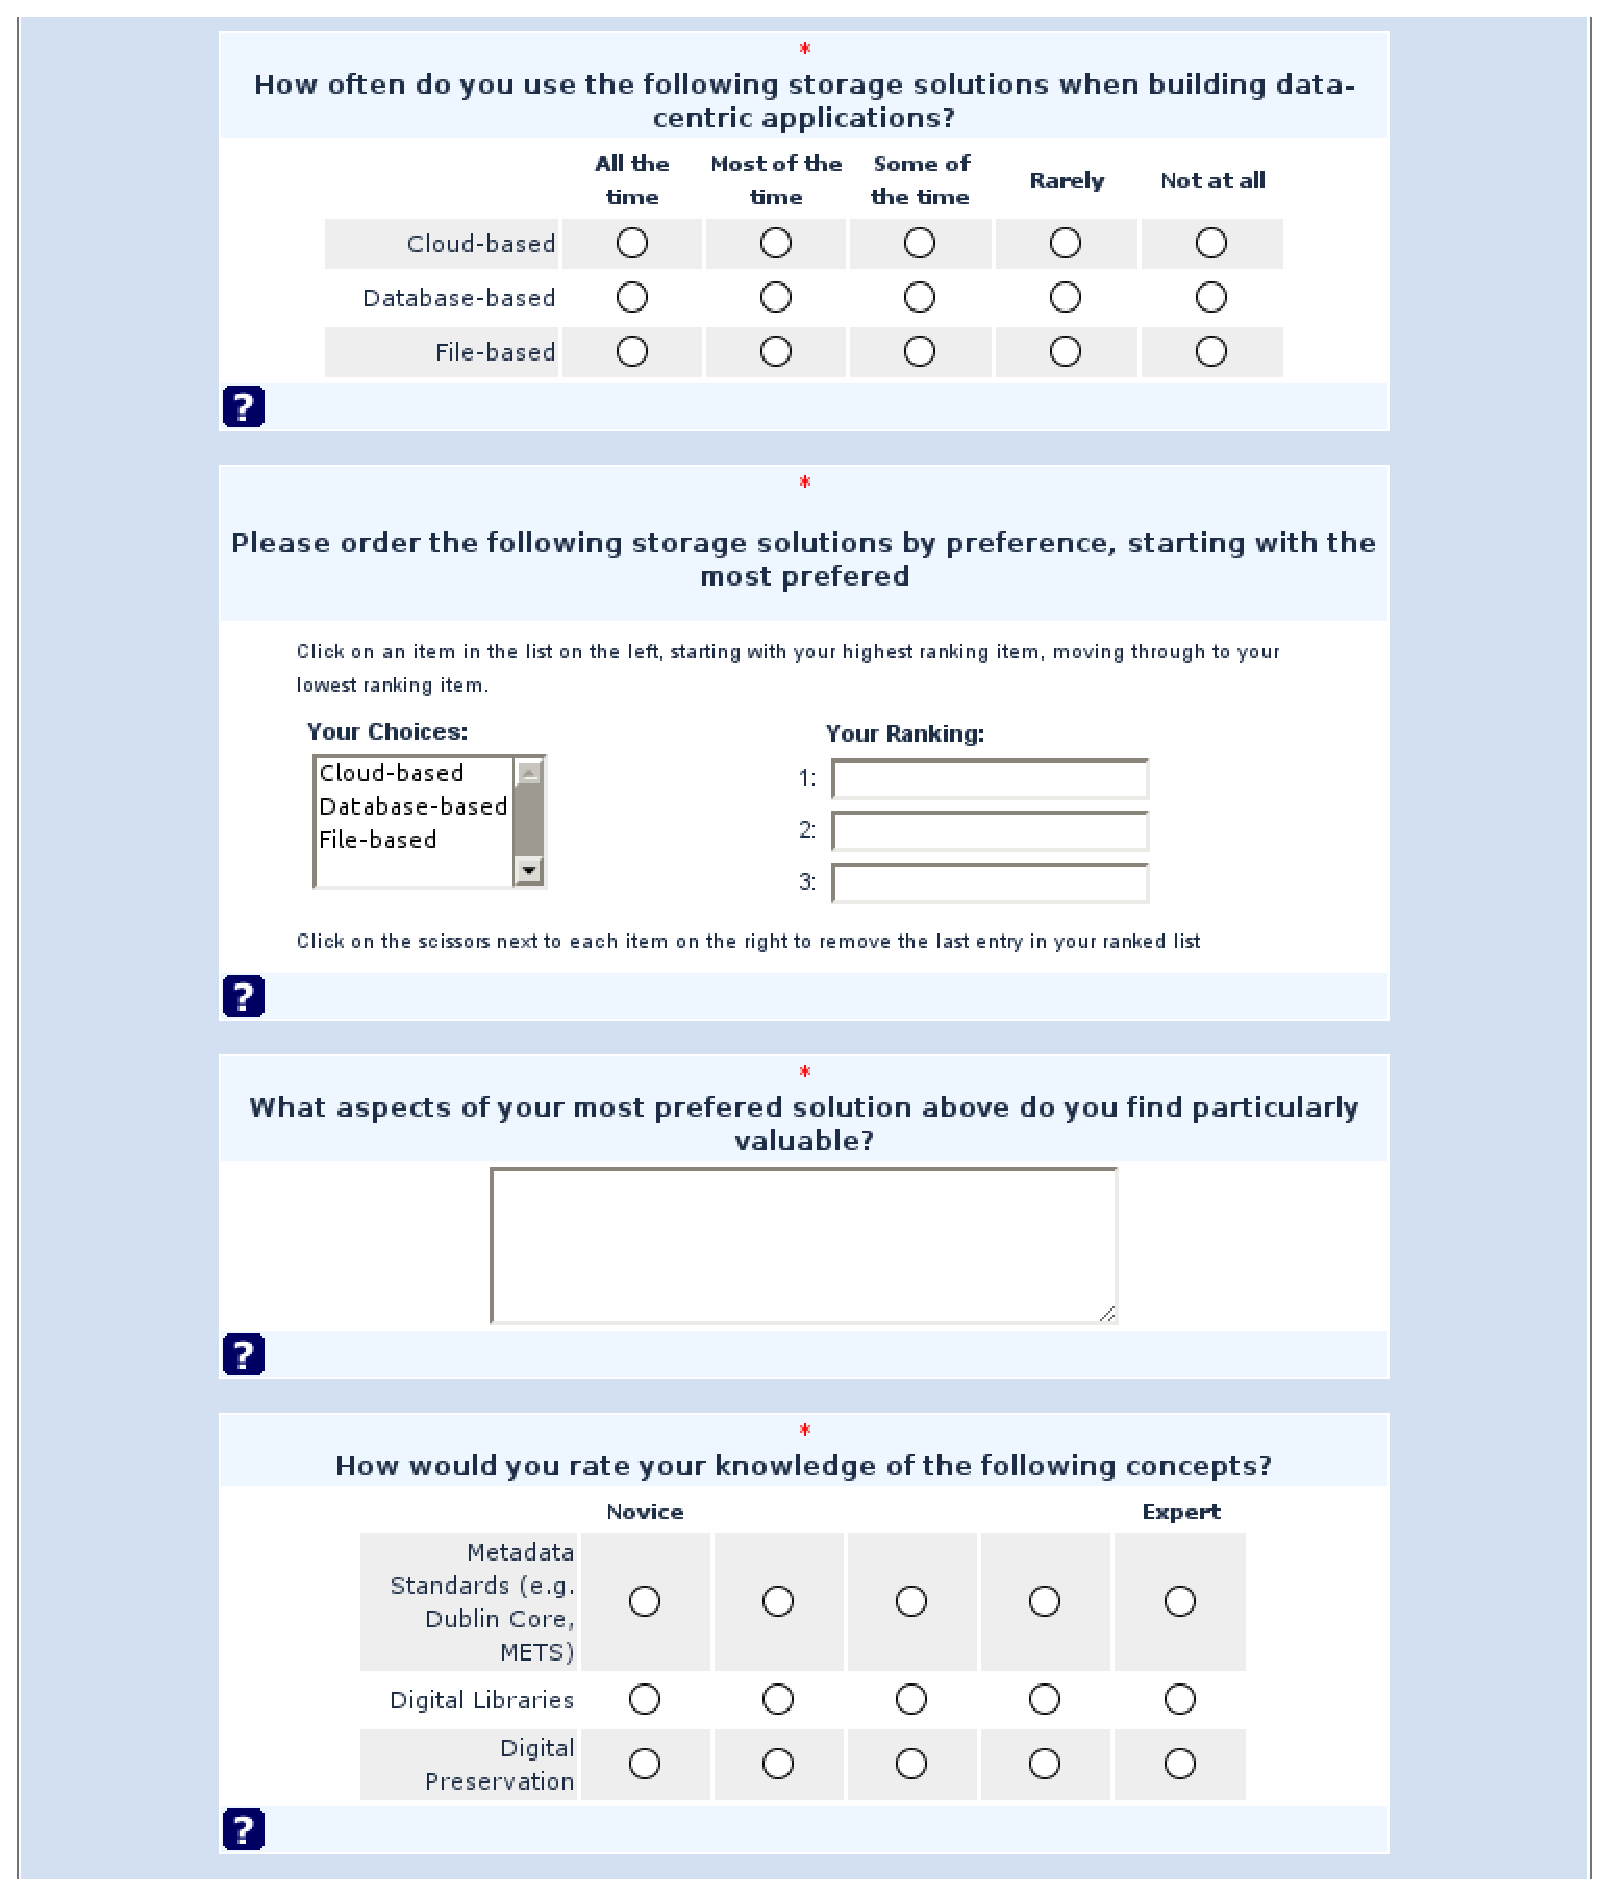
\includegraphics[width=0.95\textwidth]{appendicies/figures/developer-suvery-one-page-002.eps}
 }
 \caption[Screenshot of the online questionnaire (page 2 of 5)]{Screenshot of the online LimeSurvey questionnaire (page 2 of 5)}
 \label{appendix:appendicies:developer-suvery-one-page-002}
\end{subfigure}

\newpage

%\subsection{Section 1}
\begin{subfigure}[h]{\textwidth}
 \centering
 \framebox[\textwidth]{%
 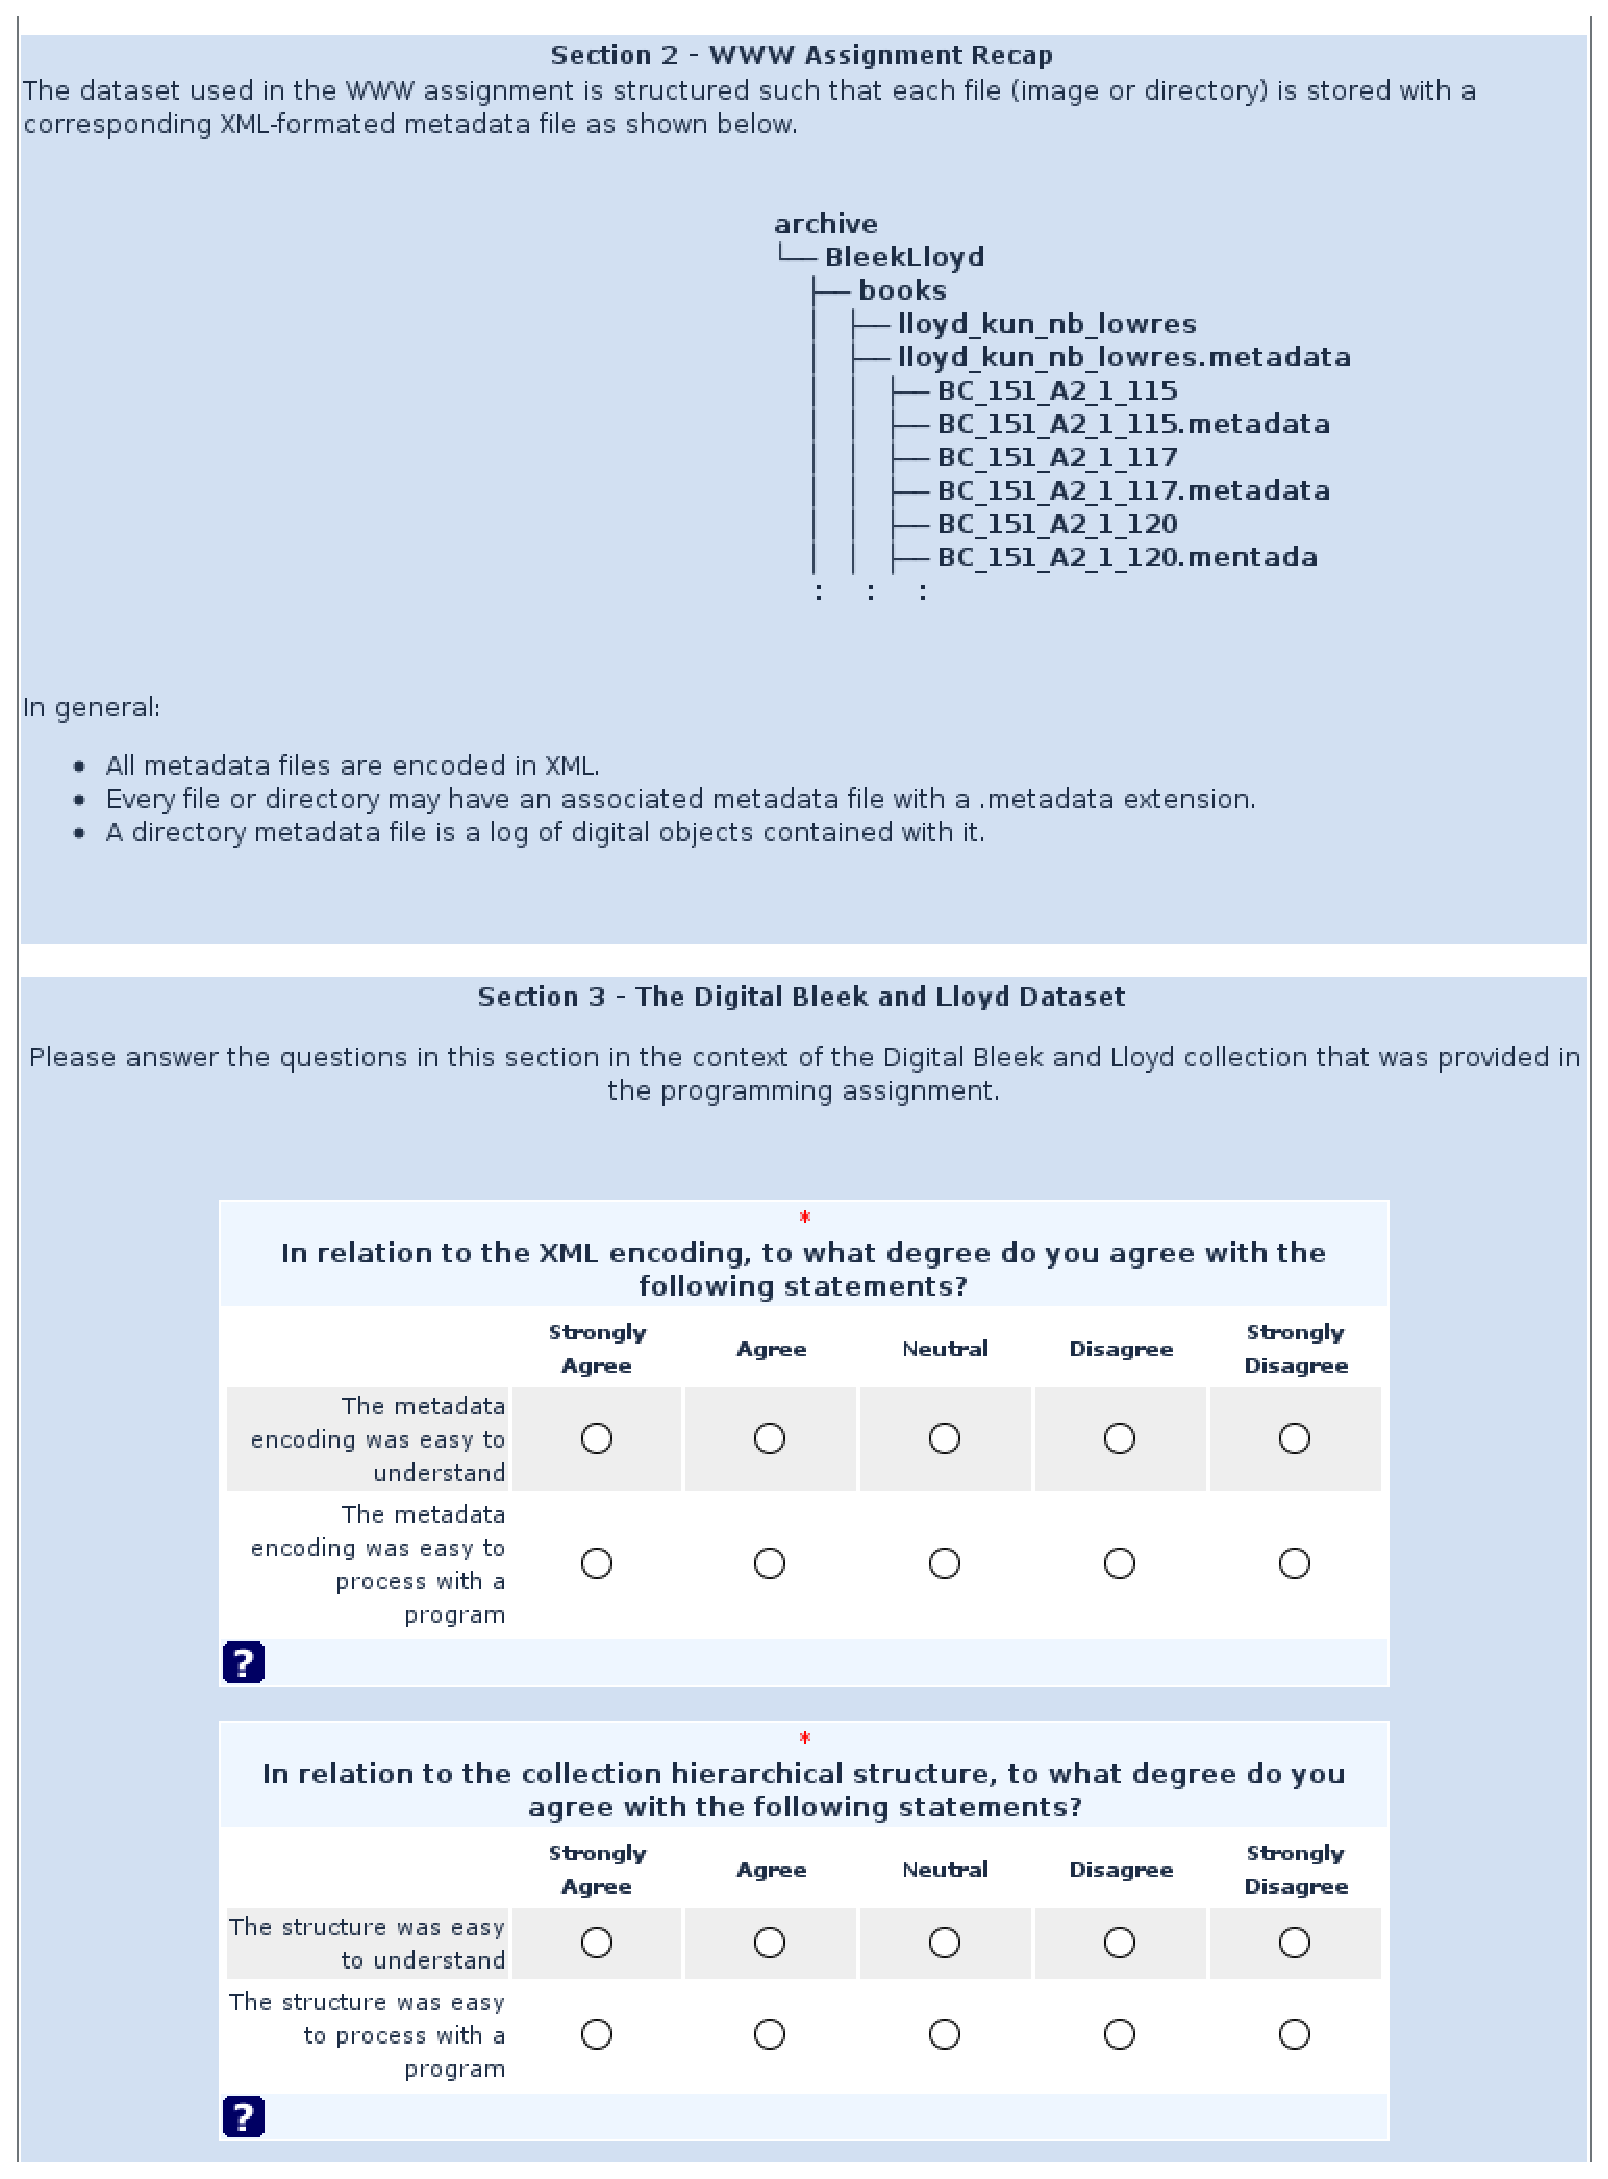
\includegraphics[width=0.95\textwidth]{appendicies/figures/developer-suvery-one-page-003.eps}
 }
 \caption[Screenshot of the online questionnaire (page 3 of 5)]{Screenshot of the online LimeSurvey questionnaire (page 3 of 5)}
 \label{appendix:appendicies:developer-suvery-one-page-003}
\end{subfigure}

\newpage

%\subsection{Section 1}
\begin{subfigure}[h]{\textwidth}
 \centering
 \framebox[\textwidth]{%
 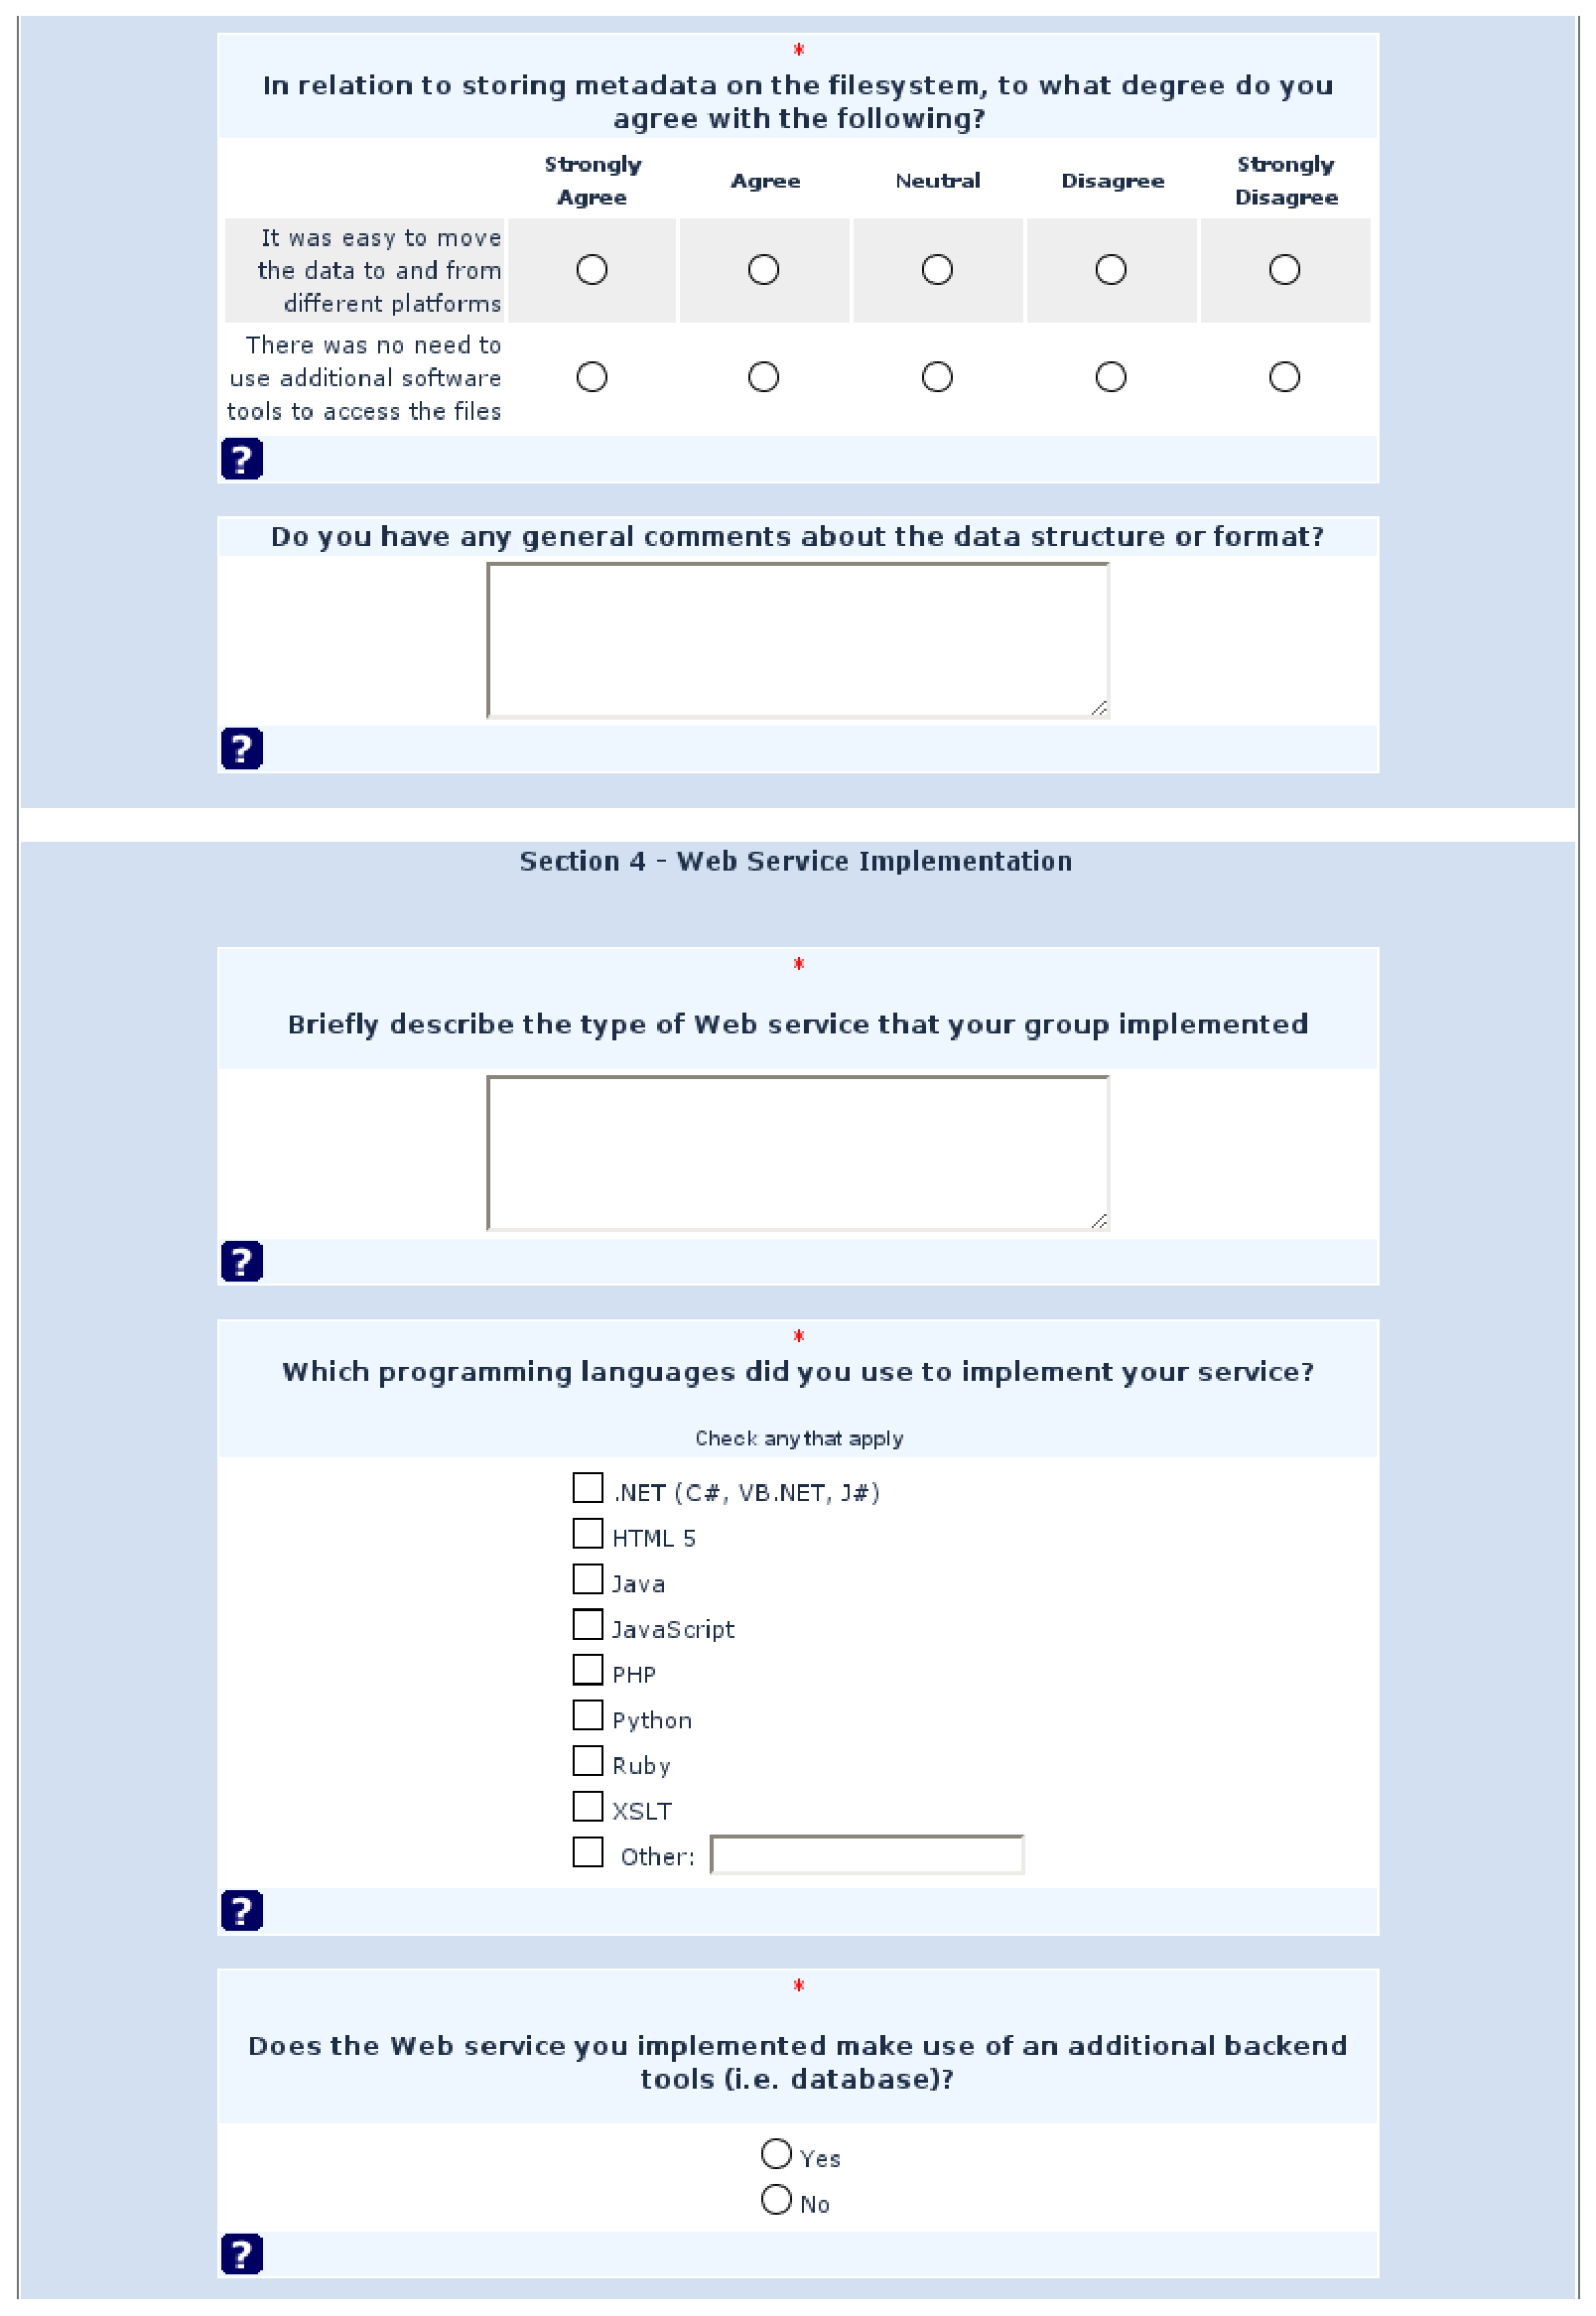
\includegraphics[width=0.95\textwidth]{appendicies/figures/developer-suvery-one-page-004.eps}
 }
 \caption[Screenshot of the online questionnaire (page 4 of 5)]{Screenshot of the online LimeSurvey questionnaire (page 4 of 5)}
 \label{appendix:appendicies:developer-suvery-one-page-004}
\end{subfigure}

\newpage

%\subsection{Section 1}
\begin{subfigure}[h]{\textwidth}
 \centering
 \framebox[\textwidth]{%
 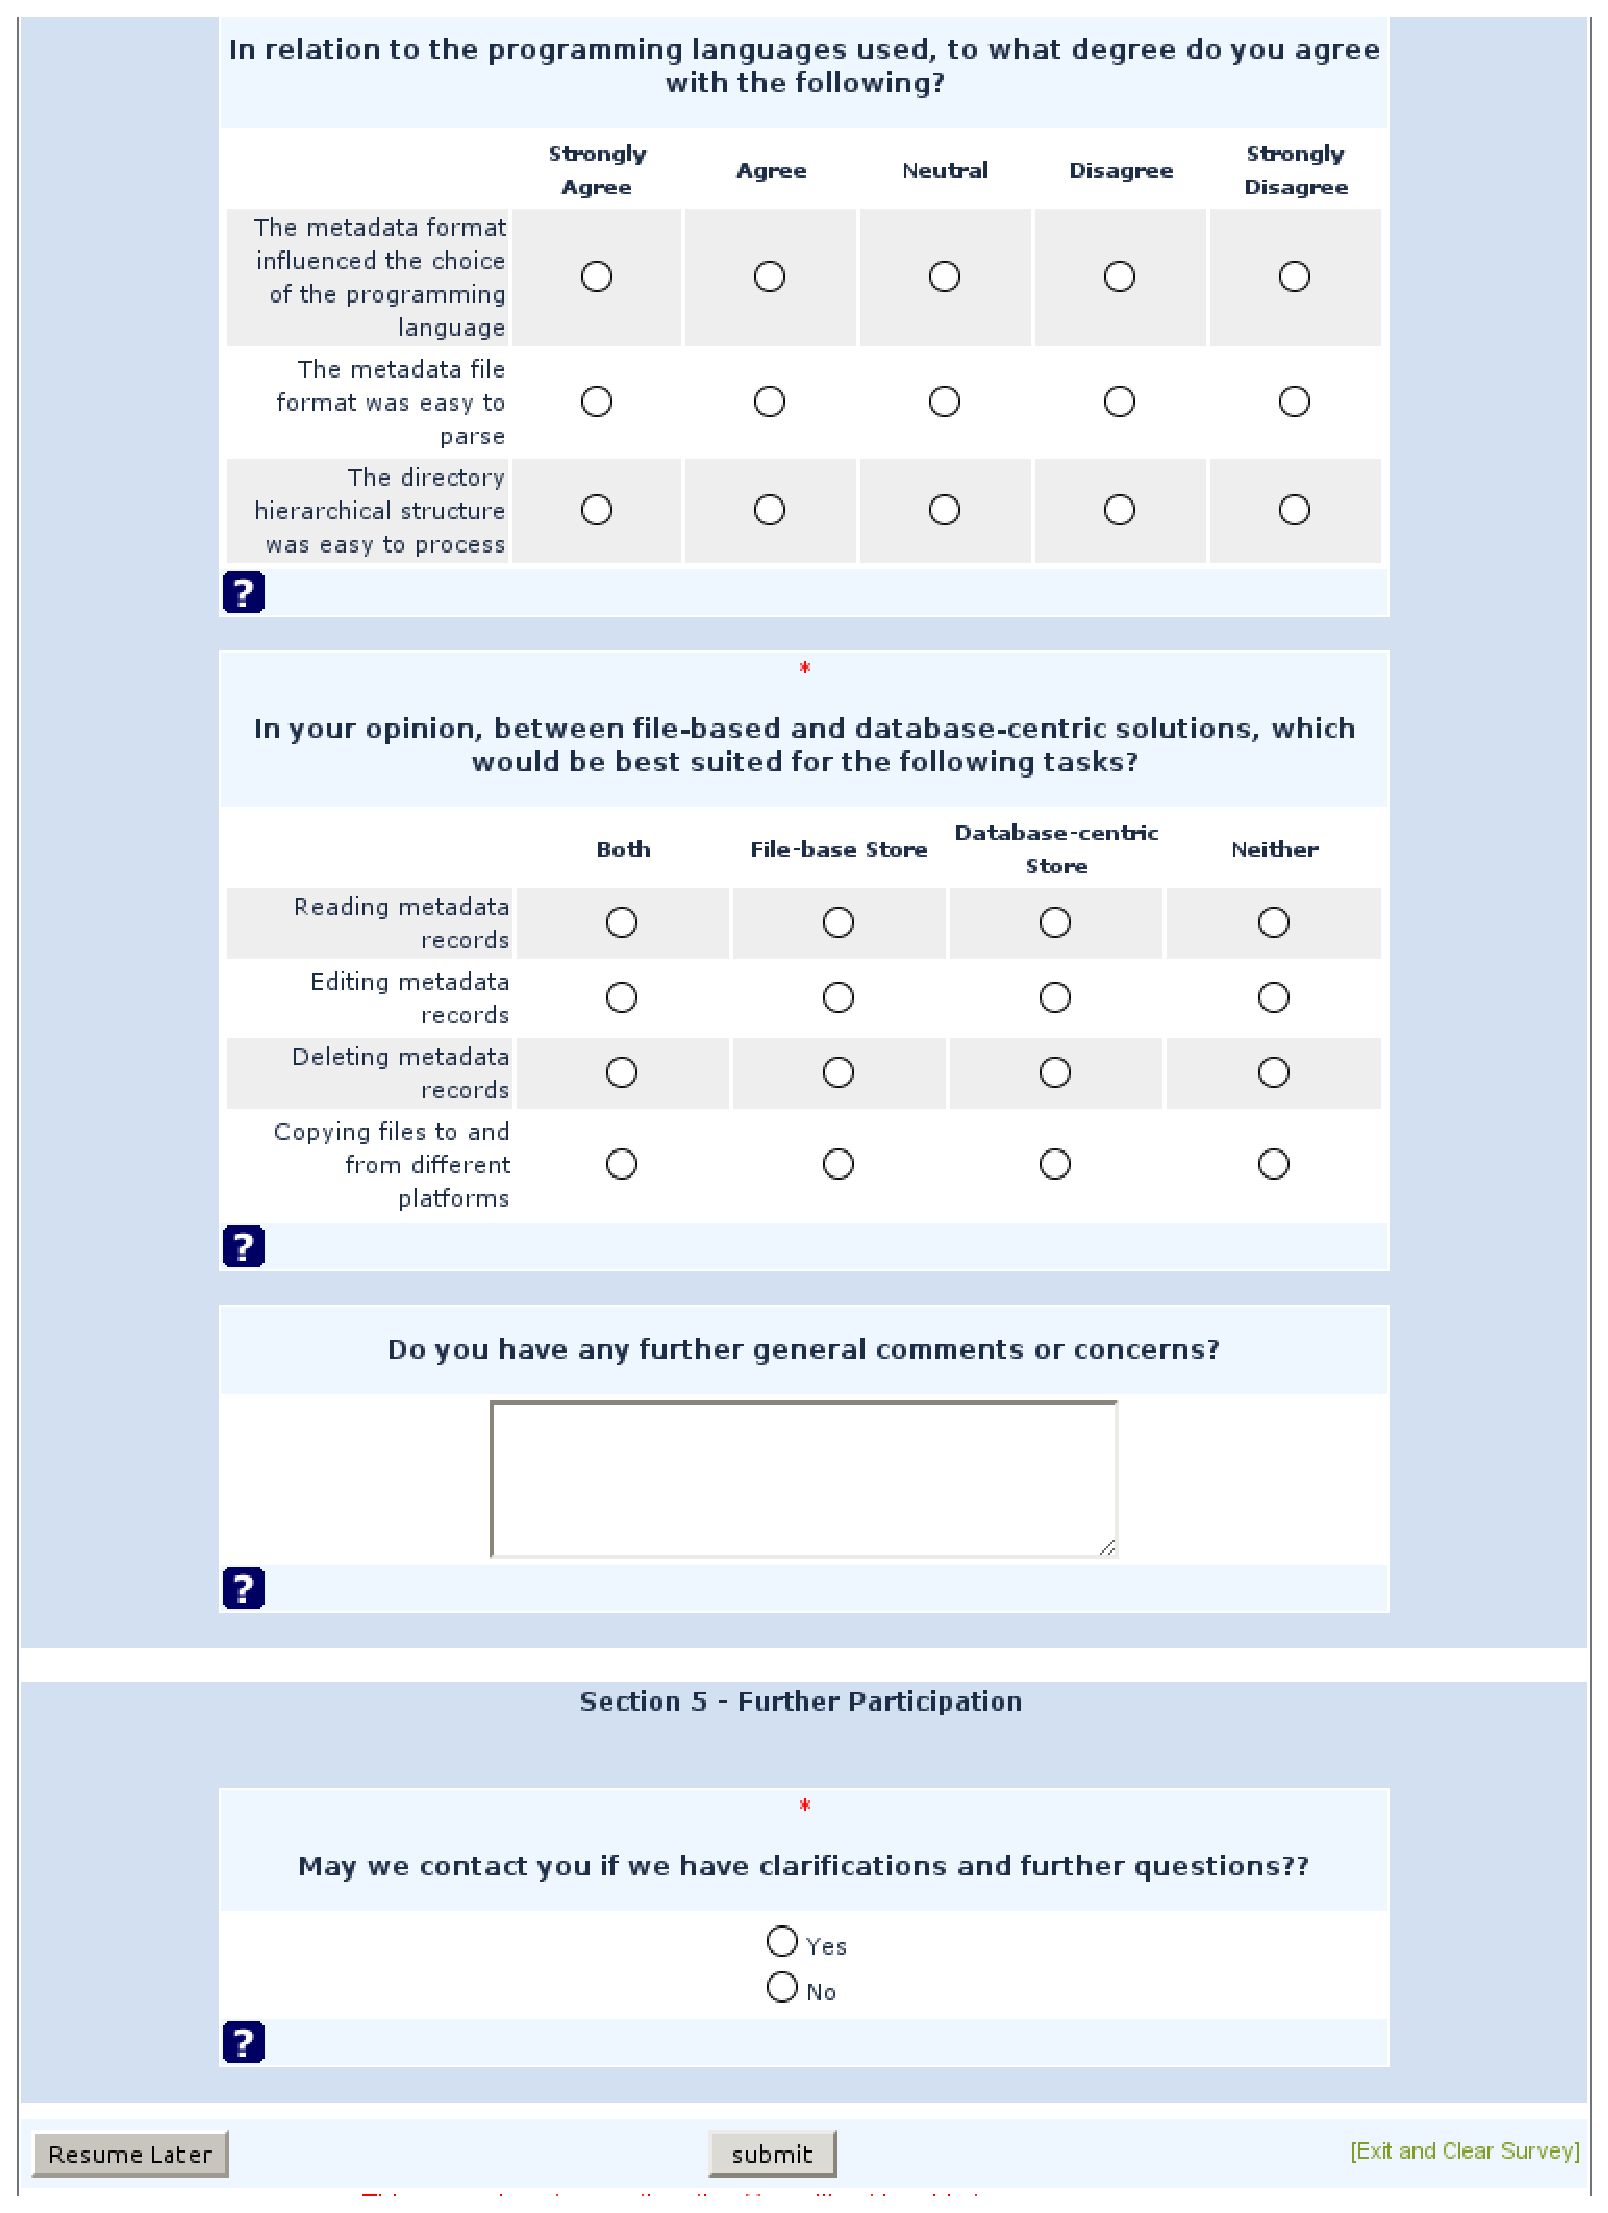
\includegraphics[width=0.95\textwidth]{appendicies/figures/developer-suvery-one-page-005.eps}
 }
 \caption[Screenshot of the online questionnaire (page 5 of 5)]{Screenshot of the online LimeSurvey questionnaire (page 5 of 5)}
 \label{appendix:appendicies:developer-suvery-one-page-005}
\end{subfigure}
 \caption[Screenshot of the online questionnaire]{Screenshot of the online LimeSurvey questionnaire}
 \label{appendix:appendicies:developer-suvery-all-in-one}
\end{figure}
\end{comment}
%%%%%%%%%%\chapter[Developer survey]{Developer survey\label{ch:appendex-c:developer-survey}}
\section{Survey design \label{ch:appendex-b:developer-survey:questionnaire-design}}

This appendix section provides auxiliary information related to the developer survey described in Section~\ref{sec:evaluation:developer-survey}. Figure~\ref{appendix:appendicies:developer-survey:WWW-survey-research-link} is a screenshot of the email sent to the target population inviting them to participate in the survey, Figure~\ref{appendix:appendicies:developer-survey:developer-survey-questionnaire1} is a screenshot of the \gls{www} practical programming assignment assigned to the target population, and Figures~\ref{appendix:appendicies:developer-suvery-one-page-001},~\ref{appendix:appendicies:developer-suvery-one-page-002},~\ref{appendix:appendicies:developer-suvery-one-page-003},~\ref{appendix:appendicies:developer-suvery-one-page-004} and~\ref{appendix:appendicies:developer-suvery-one-page-005} are screenshots of the post-assignment online questionnaire used by survey participants.

\begin{figure}
 \centering
 \framebox[\textwidth]{%
 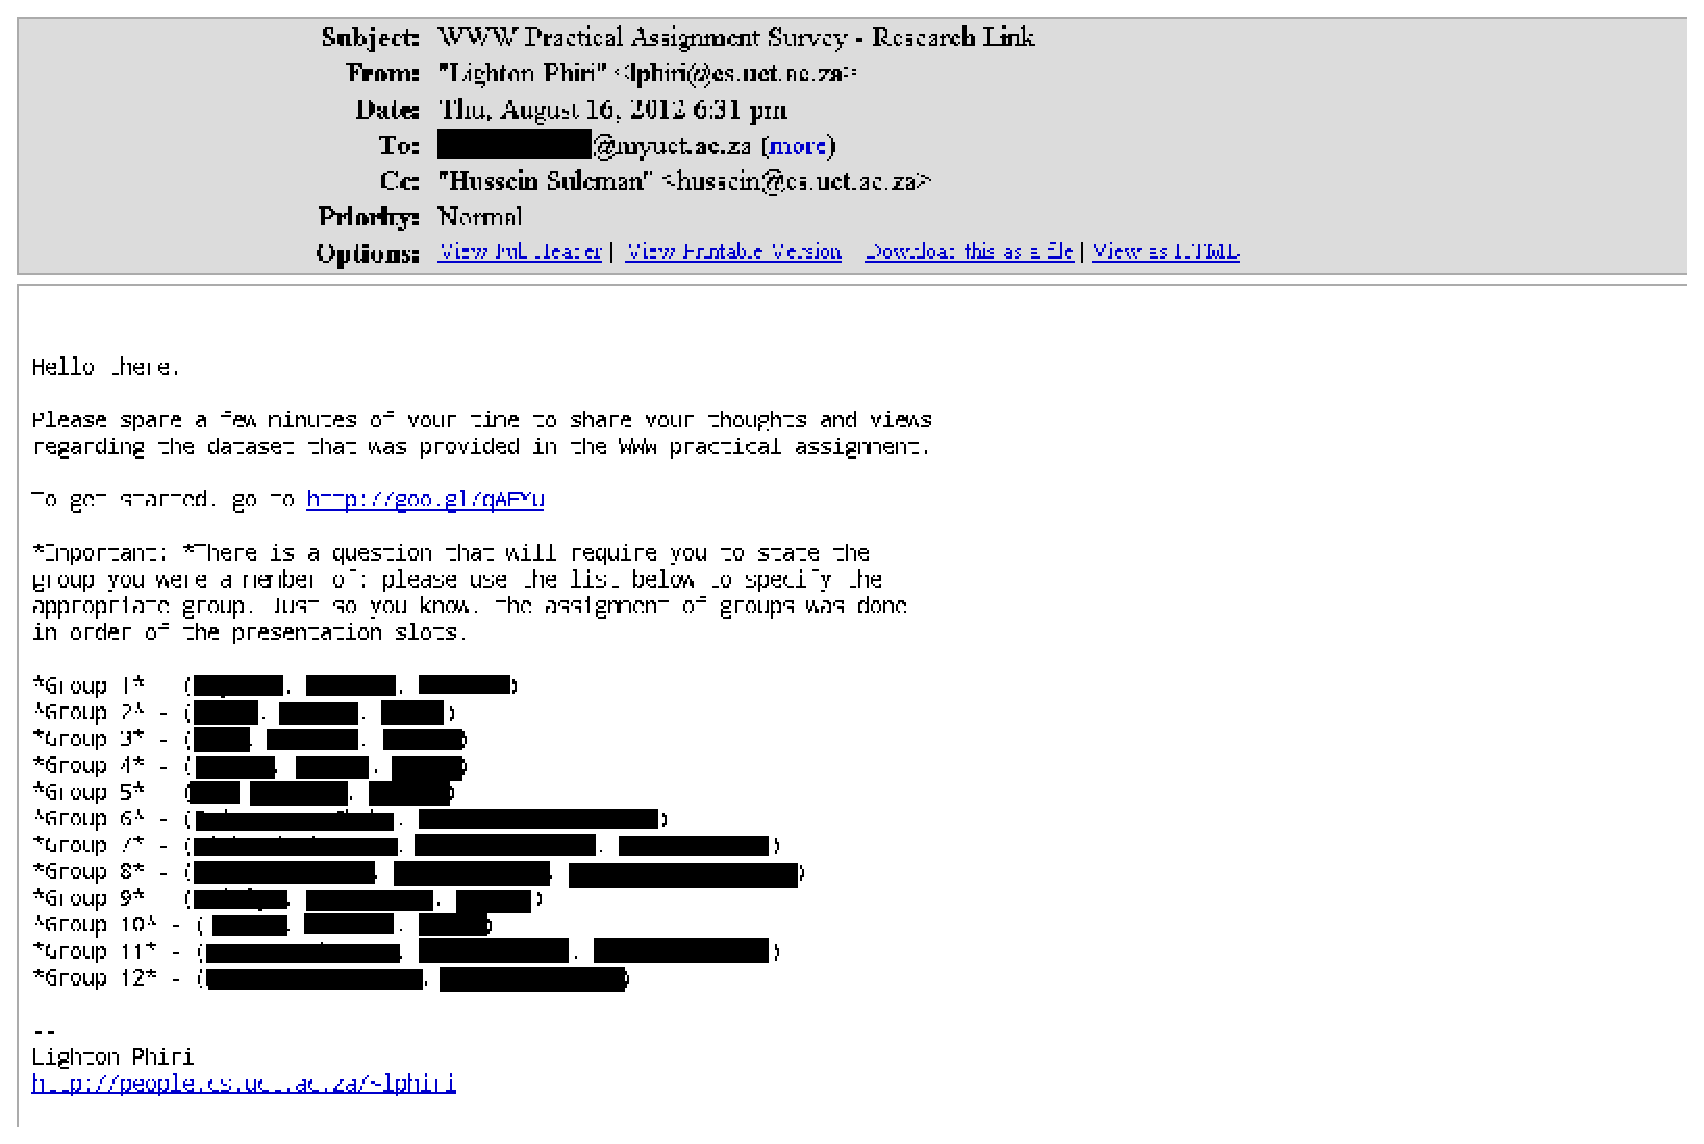
\includegraphics[width=0.95\textwidth]{appendicies/figures/WWW-survey-research-link-masked.eps}
 }
 \caption[Screenshot showing the survey participation email invitation]{Screenshot showing the WWW survey participation email invitation}
 \label{appendix:appendicies:developer-survey:WWW-survey-research-link}
\end{figure}

%\subsection{Section 1}
\begin{figure}
 \centering
 \framebox[\textwidth]{%
 \includegraphics[width=0.95\textwidth]{appendicies/figures/developer-assignment-question-screenshot.eps}
 }
 \caption[Screenshot showing the practical assignment question]{Screenshot showing the WWW practical programming assignment question}
 \label{appendix:appendicies:developer-survey:developer-survey-questionnaire1}
\end{figure}


% 
% subfigure and subfig packages deprecated
% http://en.wikibooks.org/wiki/LaTeX/Floats,_Figures_and_Captions#Subfloats

%\subsection{Section 1}
\begin{figure}
 \centering
 \subfloat[][]{%
 \framebox[\textwidth]{%
 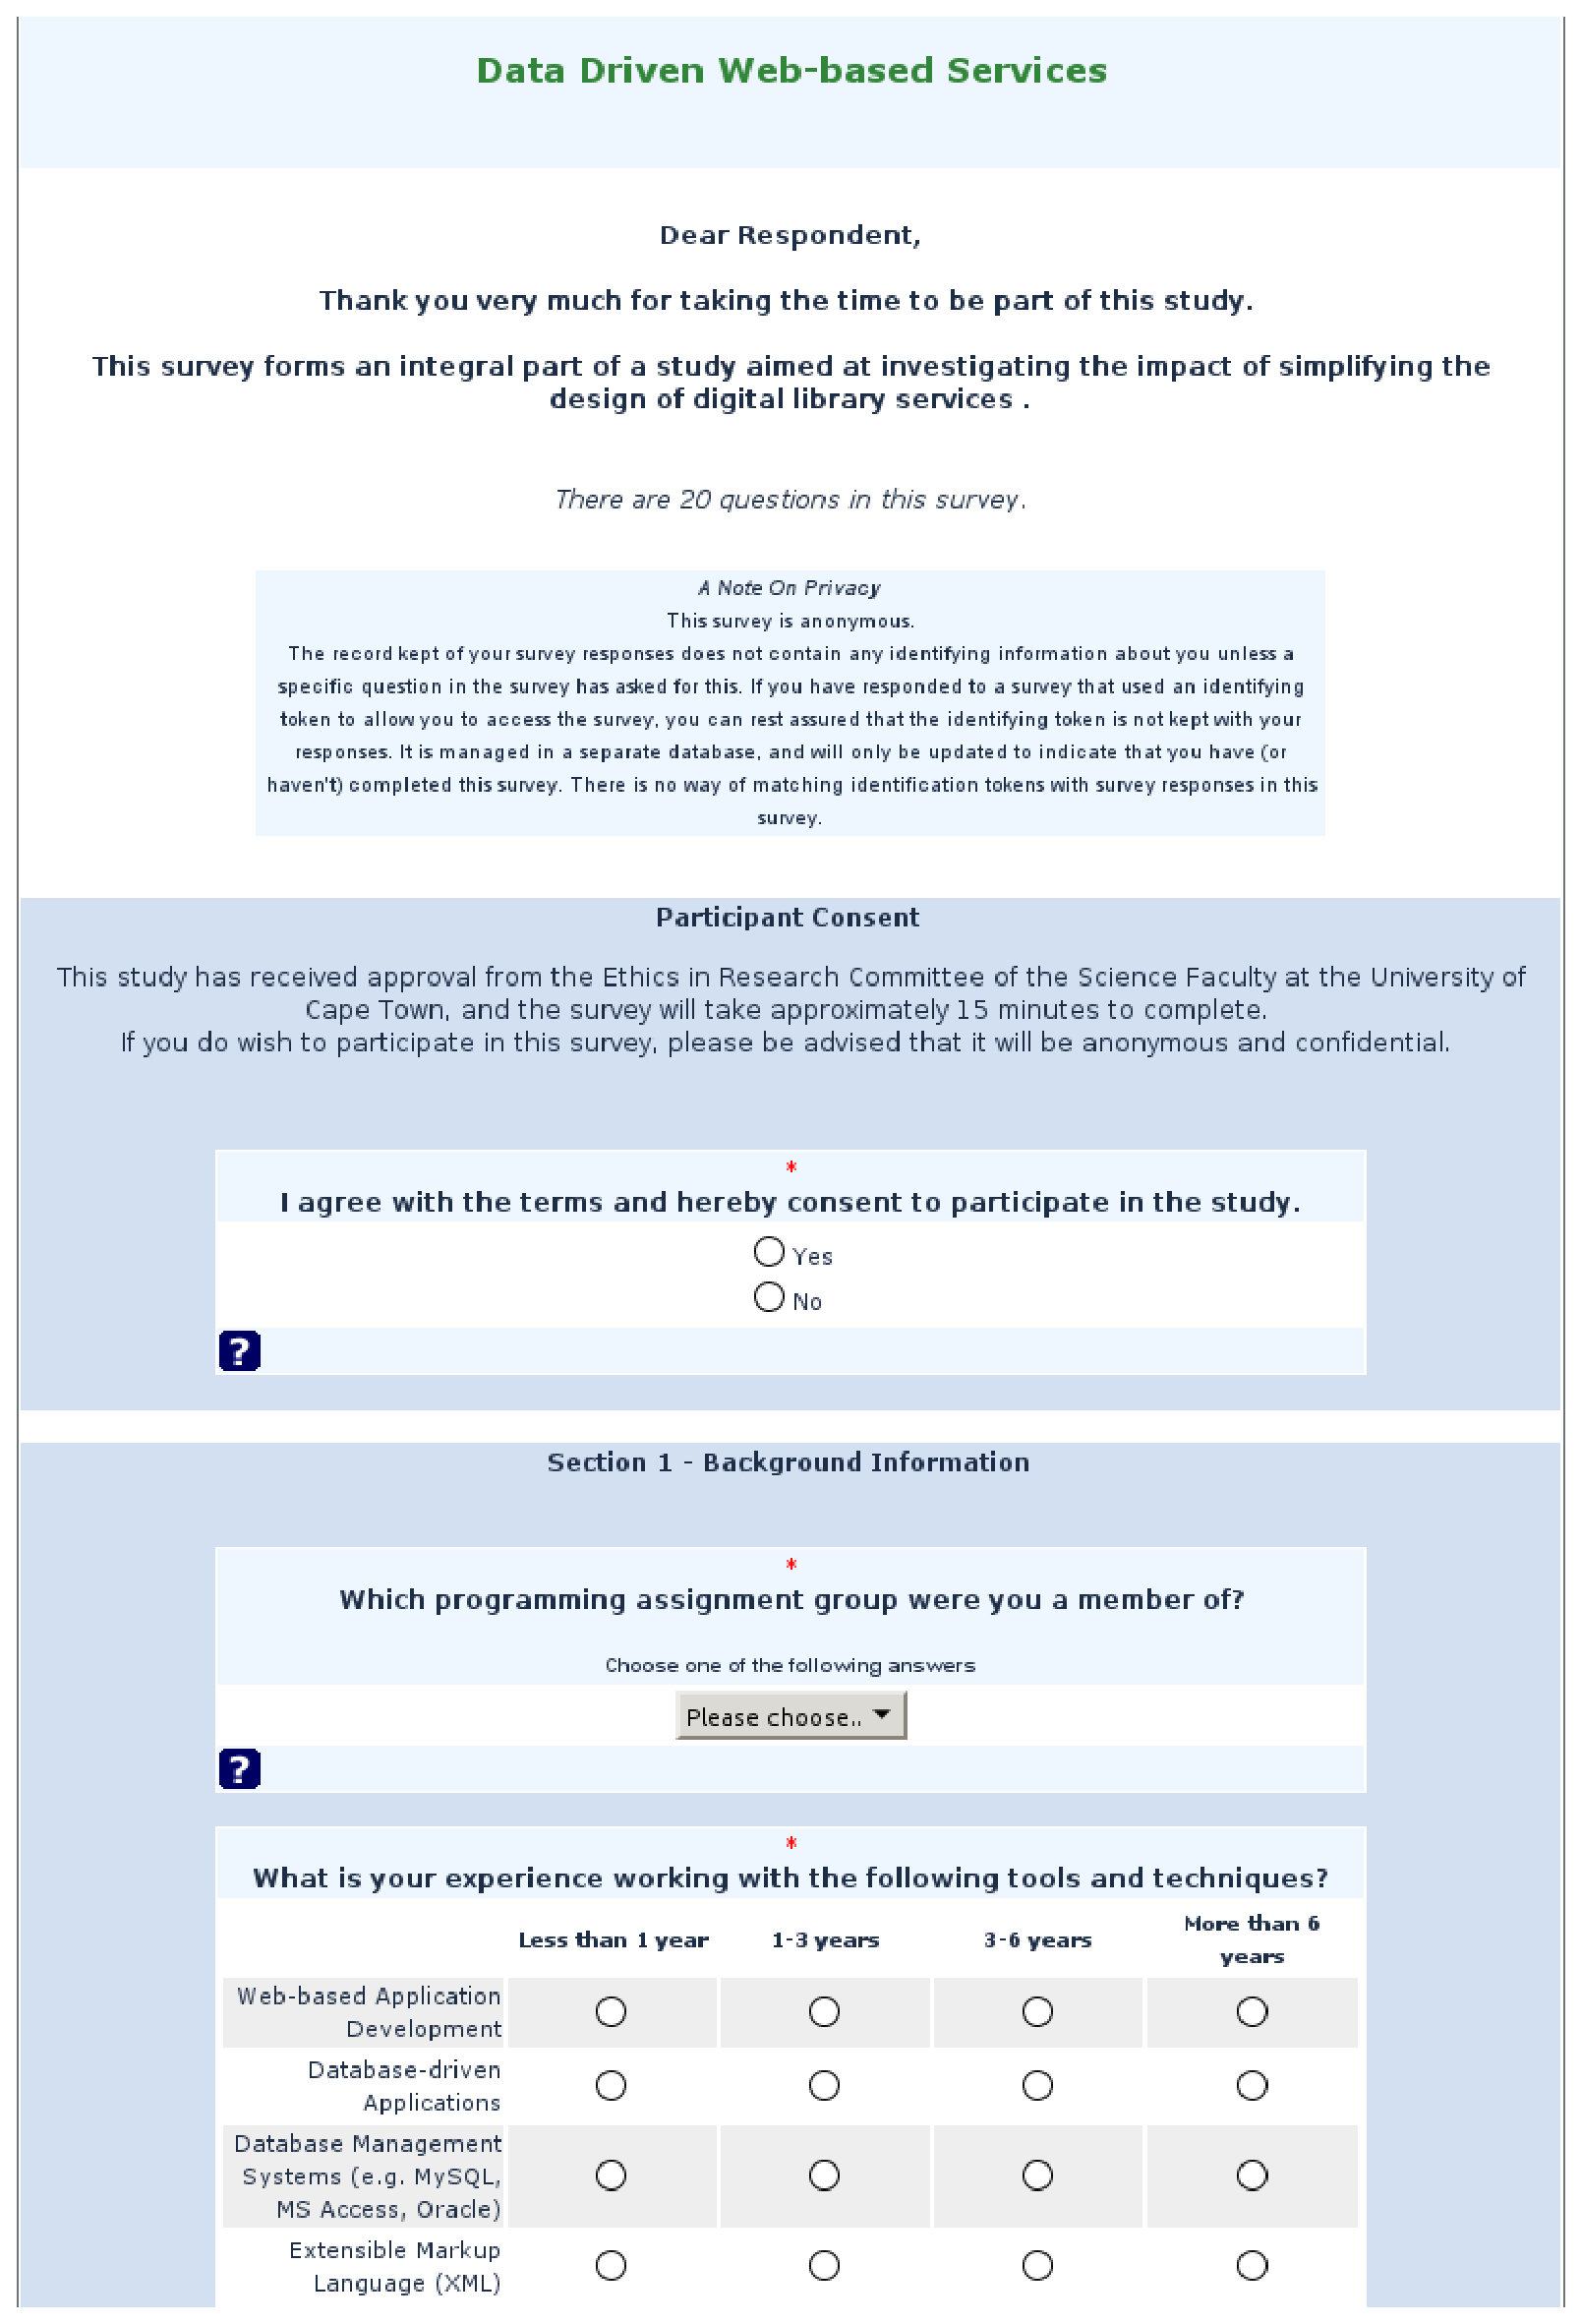
\includegraphics[width=0.95\textwidth]{appendicies/figures/developer-suvery-one-page-001.eps}
 }
 }
 \caption[Screenshot showing the online questionnaire (page 1 of 5)]{Screenshot showing the online LimeSurvey questionnaire (page 1 of 5)}
 \label{appendix:appendicies:developer-suvery-one-page-001}
\end{figure}

%\subsection{Section 1}
\begin{figure}
\ContinuedFloat
 \centering
 \subfloat[][]{%
 \framebox[\textwidth]{%
 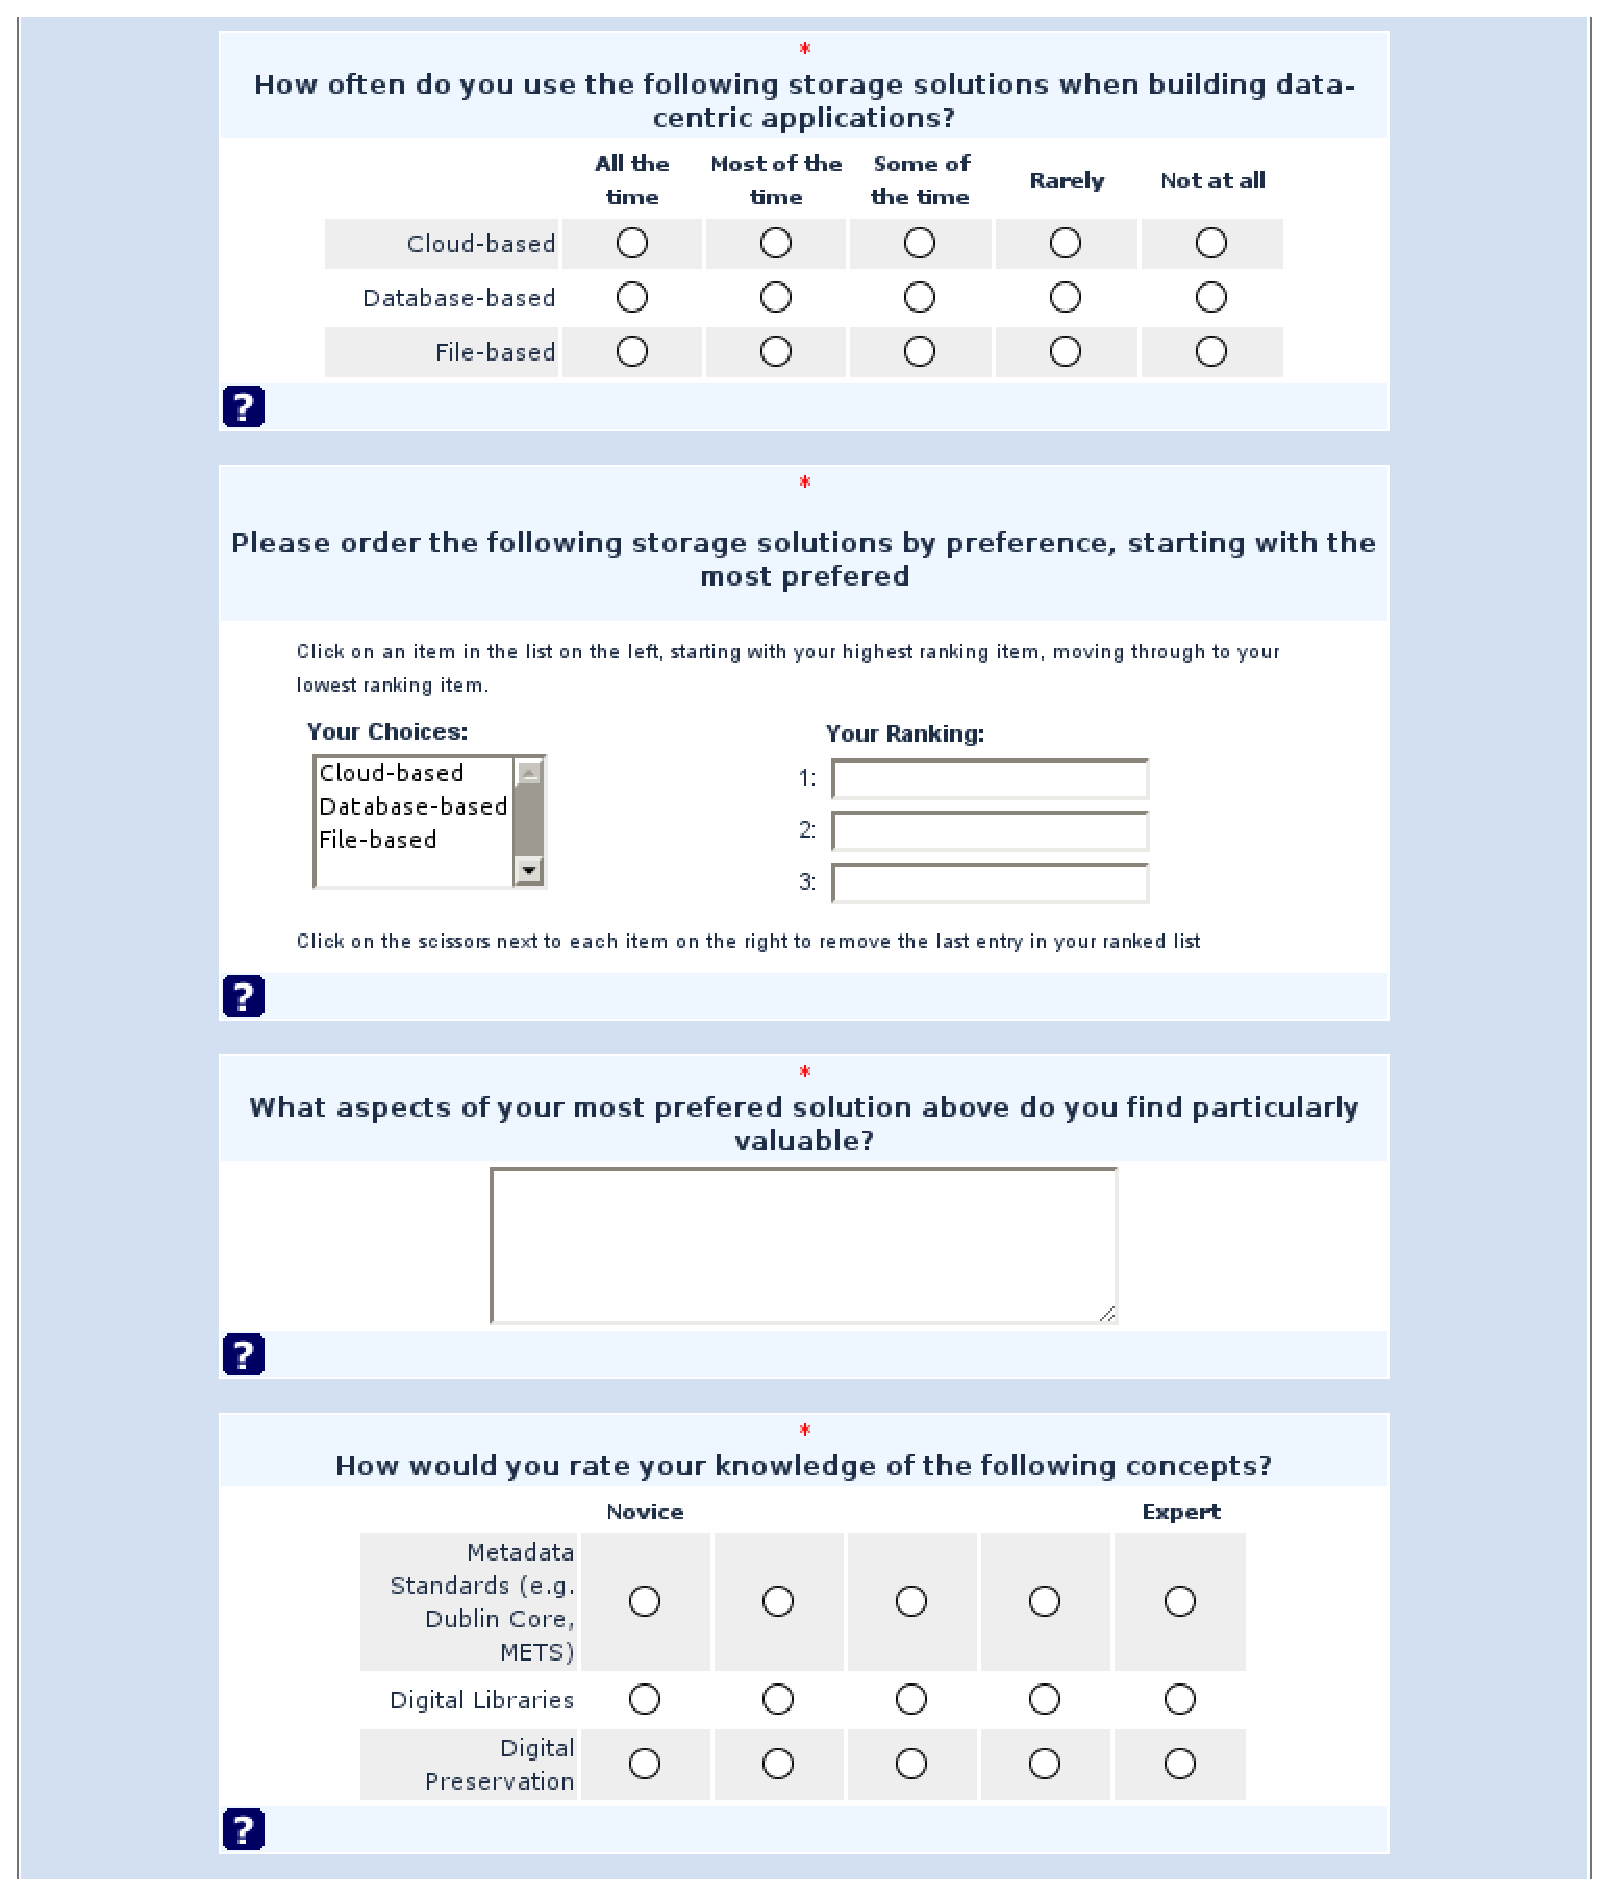
\includegraphics[width=0.95\textwidth]{appendicies/figures/developer-suvery-one-page-002.eps}
 }
 }
 \caption[Screenshot showing the online questionnaire (page 2 of 5)]{Screenshot showing the online LimeSurvey questionnaire (page 2 of 5)}
 \label{appendix:appendicies:developer-suvery-one-page-002}
\end{figure}


%\subsection{Section 1}
\begin{figure}
\ContinuedFloat
 \centering
 \subfloat[][]{%
 \framebox[\textwidth]{%
 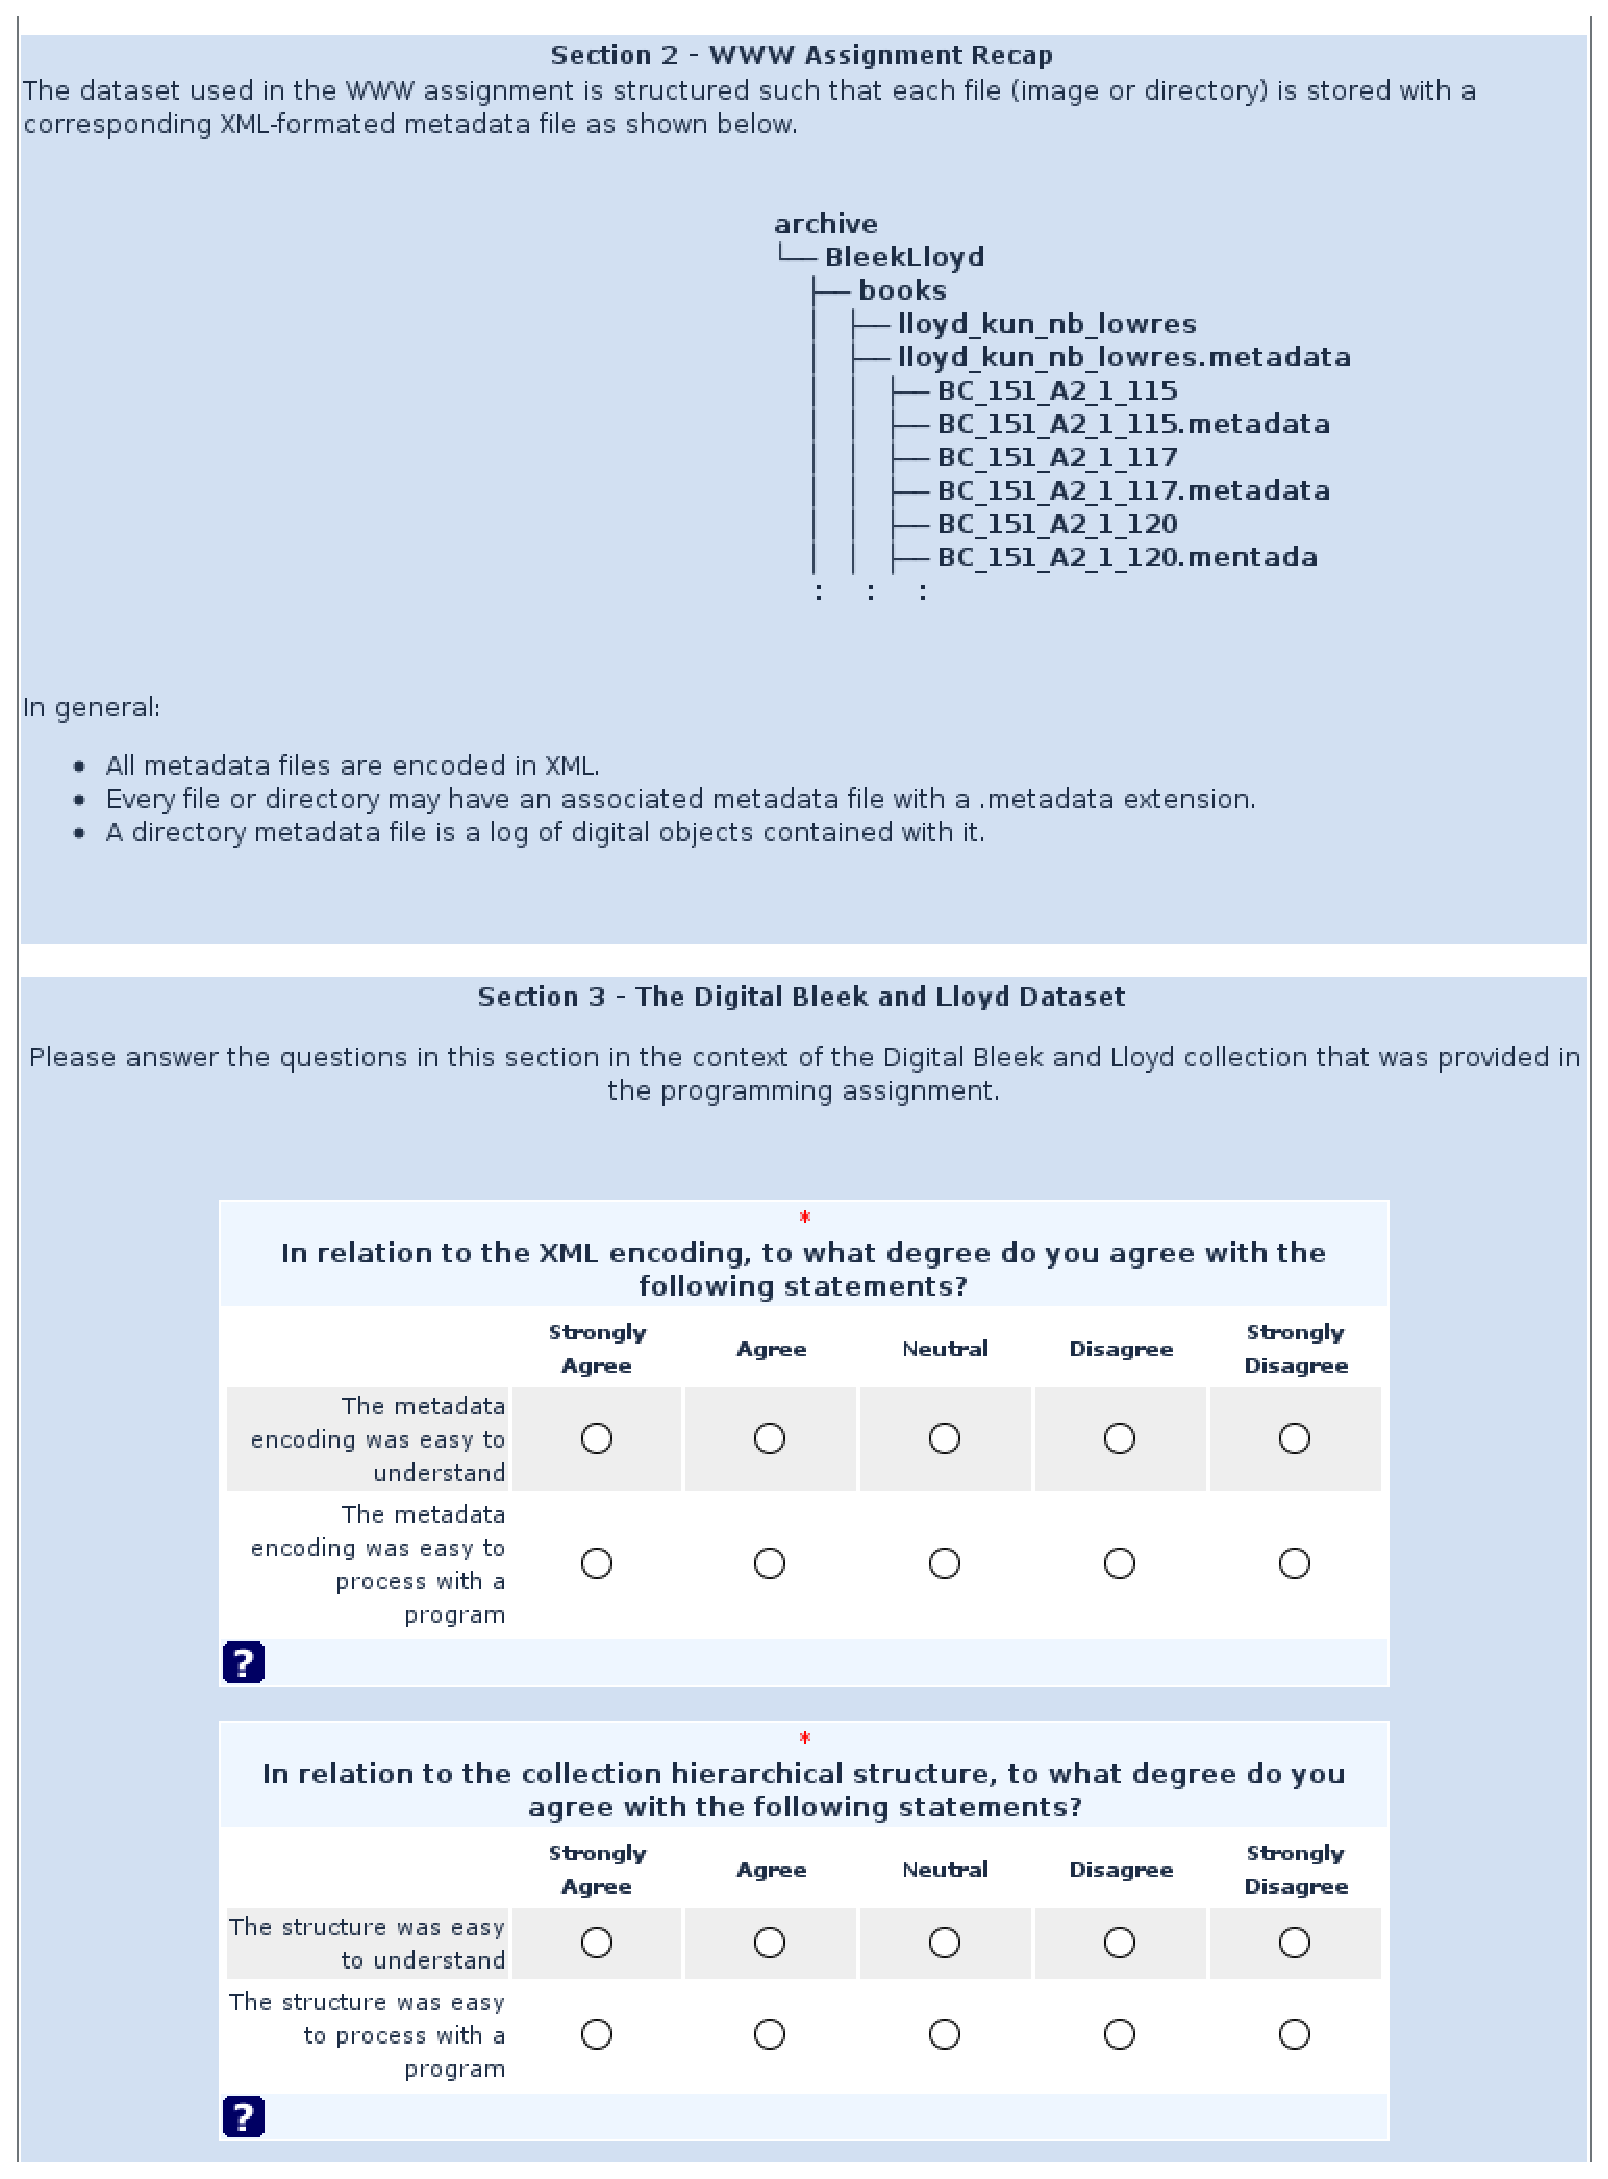
\includegraphics[width=0.95\textwidth]{appendicies/figures/developer-suvery-one-page-003.eps}
 }
 }
 \caption[Screenshot showing the online questionnaire (page 3 of 5)]{Screenshot showing the online LimeSurvey questionnaire (page 3 of 5)}
 \label{appendix:appendicies:developer-suvery-one-page-003}
\end{figure}


%\subsection{Section 1}
\begin{figure}
\ContinuedFloat
 \centering
 \subfloat[][]{%
 \framebox[\textwidth]{%
 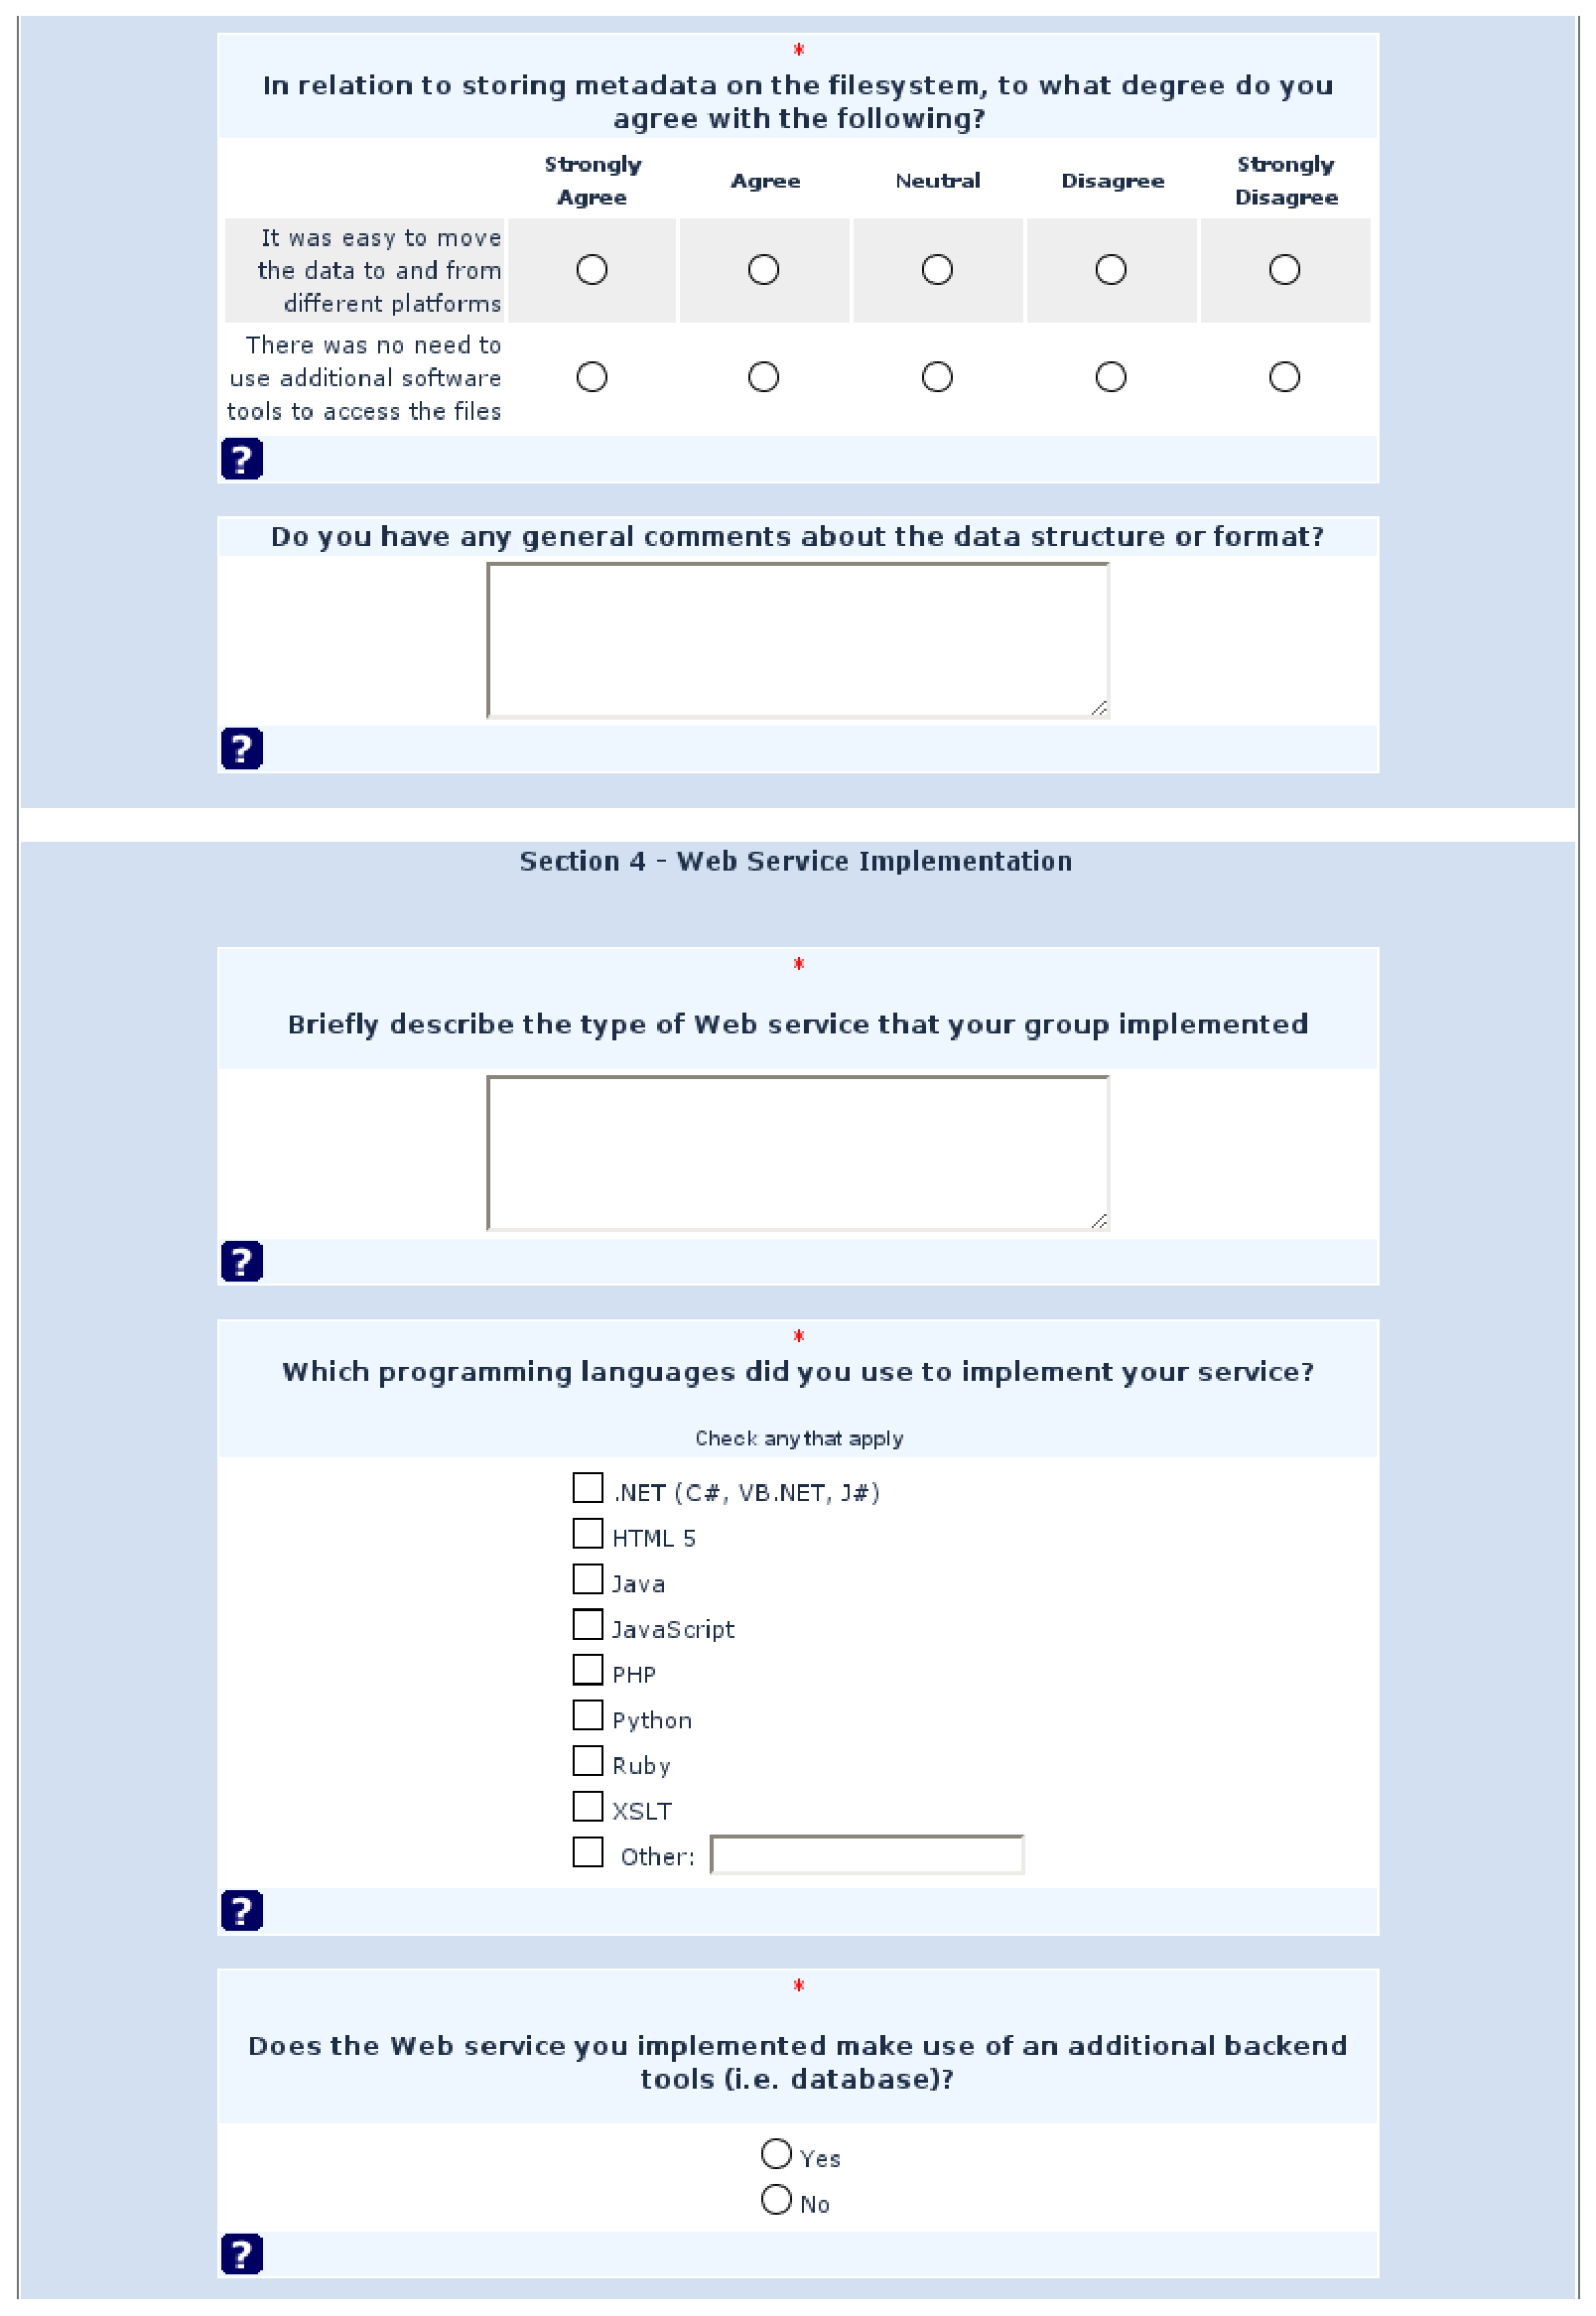
\includegraphics[width=0.95\textwidth]{appendicies/figures/developer-suvery-one-page-004.eps}
 }
 }
 \caption[Screenshot showing the online questionnaire (page 4 of 5)]{Screenshot showing the online LimeSurvey questionnaire (page 4 of 5)}
 \label{appendix:appendicies:developer-suvery-one-page-004}
\end{figure}


%\subsection{Section 1}
\begin{figure}
\ContinuedFloat
 \centering
 \subfloat[][]{%
 \framebox[\textwidth]{%
 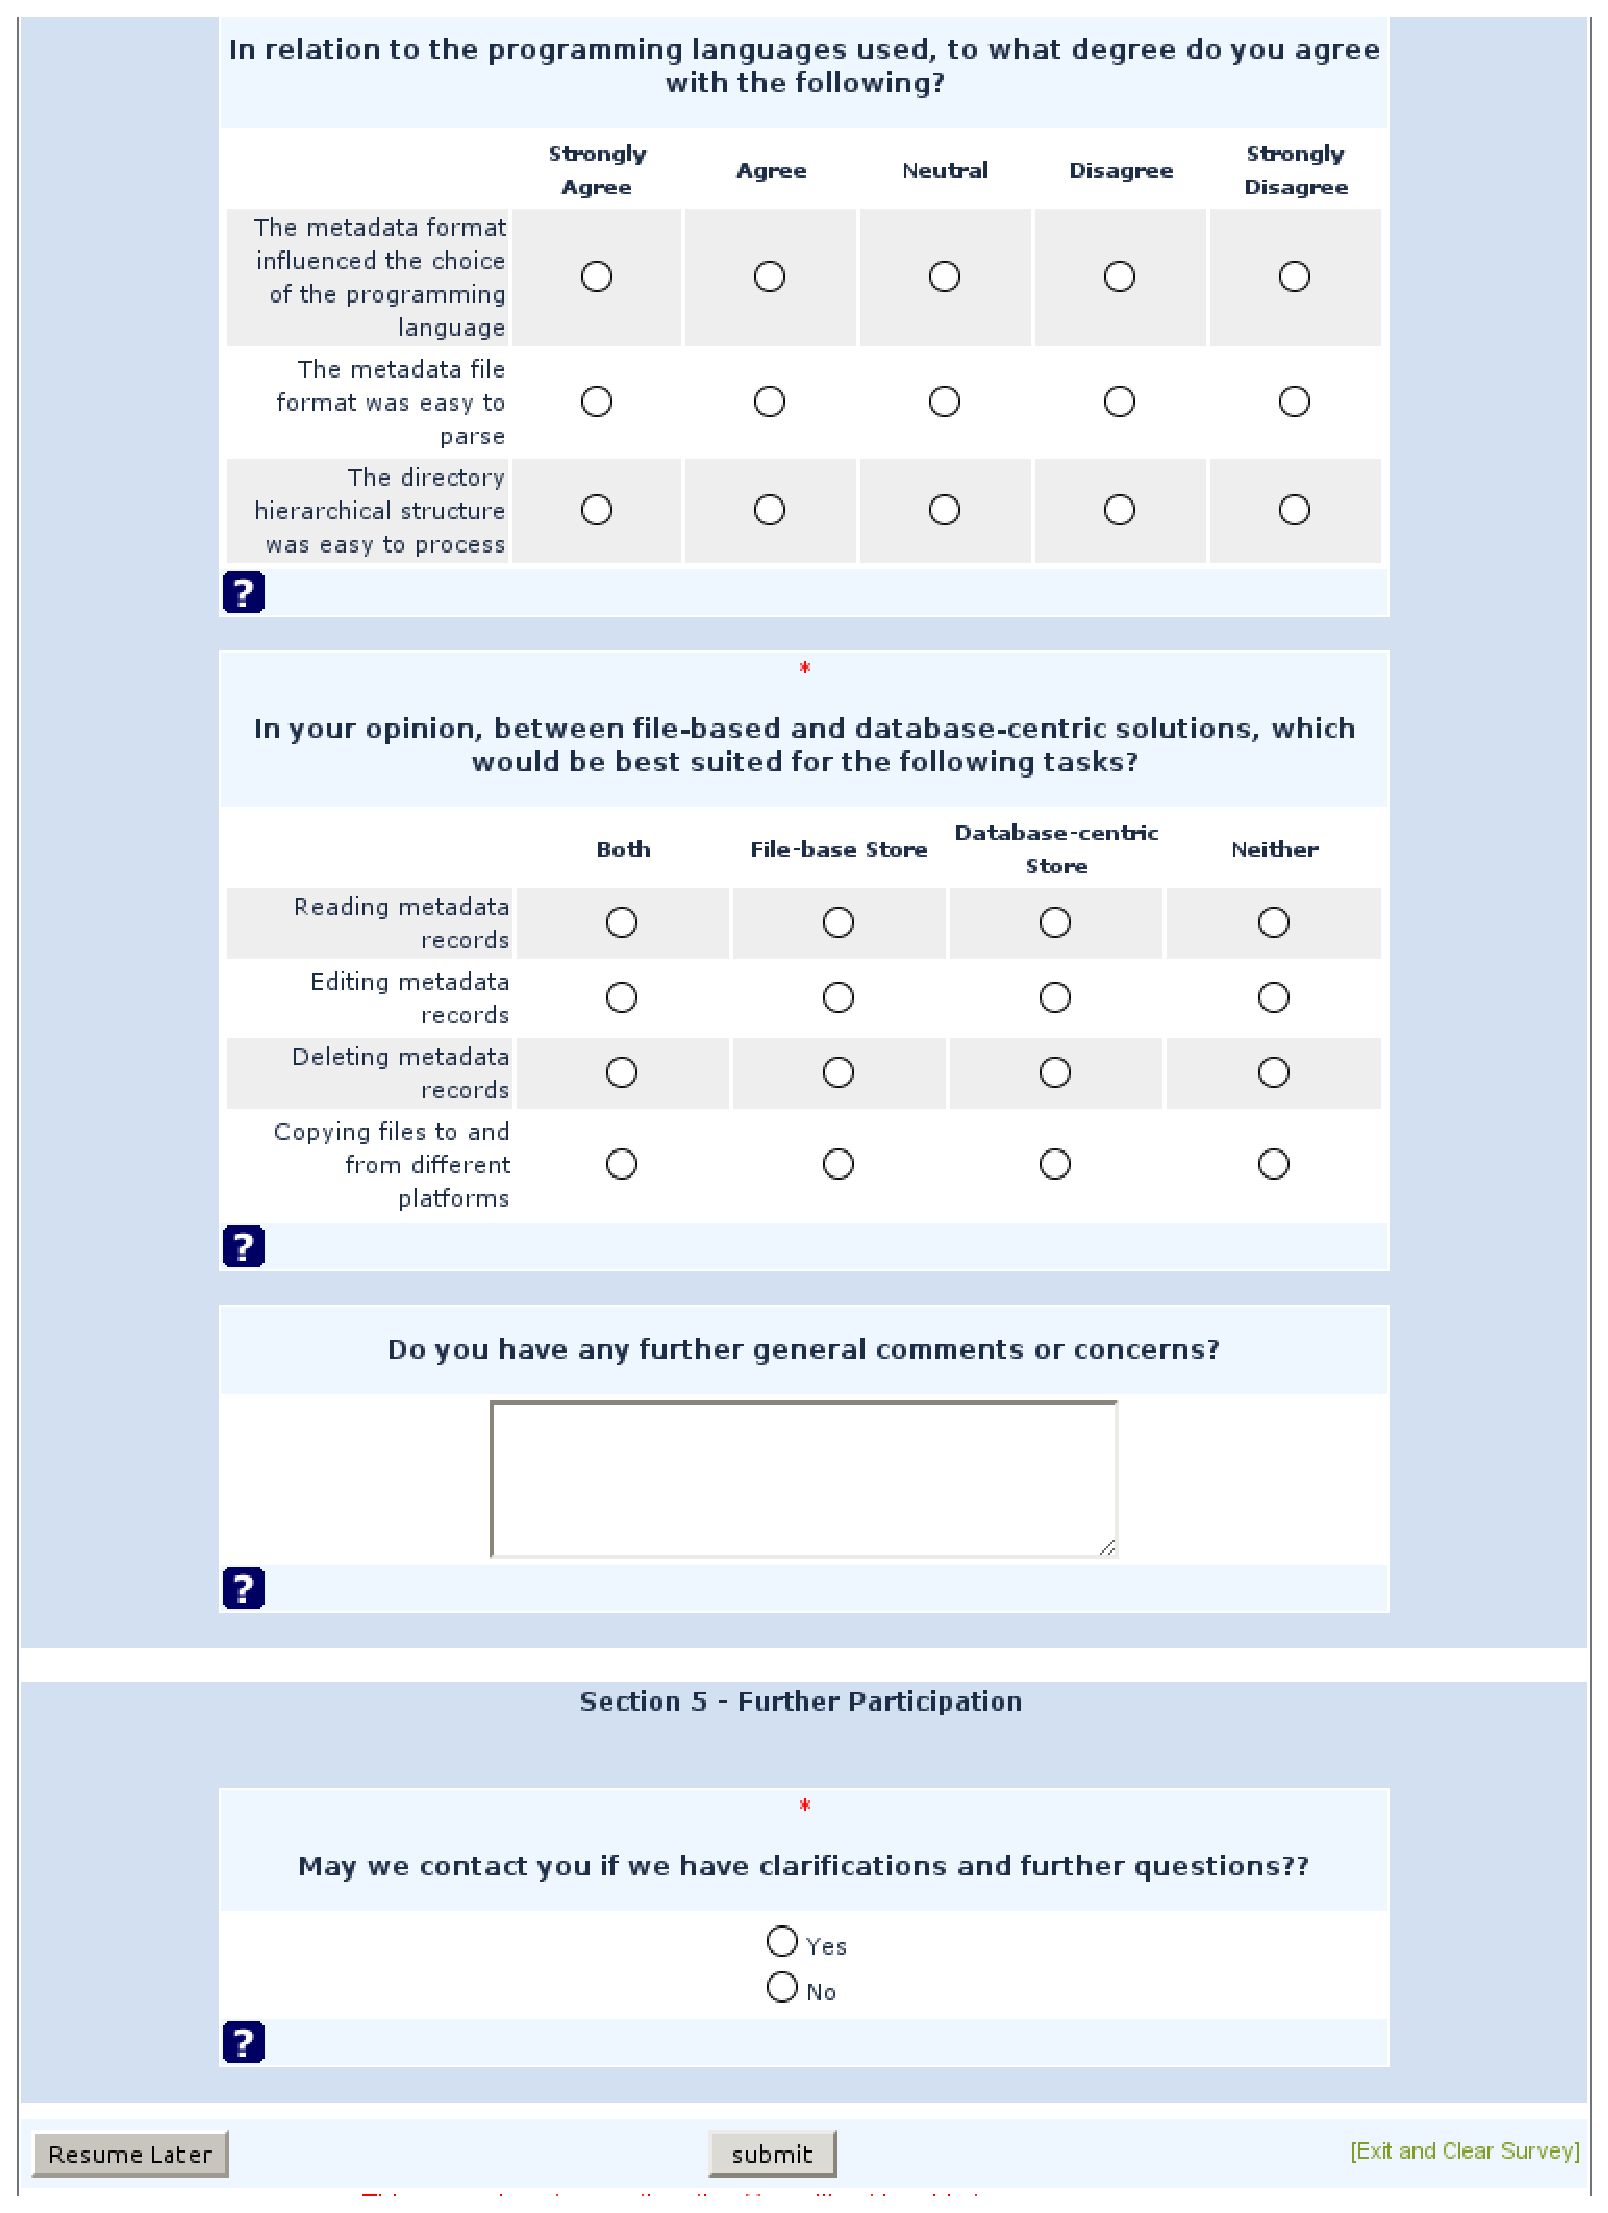
\includegraphics[width=0.95\textwidth]{appendicies/figures/developer-suvery-one-page-005.eps}
 }
 }
 \caption[Screenshot showing the online questionnaire (page 5 of 5)]{Screenshot showing the online LimeSurvey questionnaire (page 5 of 5)}
 \label{appendix:appendicies:developer-suvery-one-page-005}
\end{figure}


\begin{comment}
\begin{figure}
%\subsection{Section 1}
\begin{subfigure}[b]{\textwidth}
 \centering
 \framebox[\textwidth]{%
 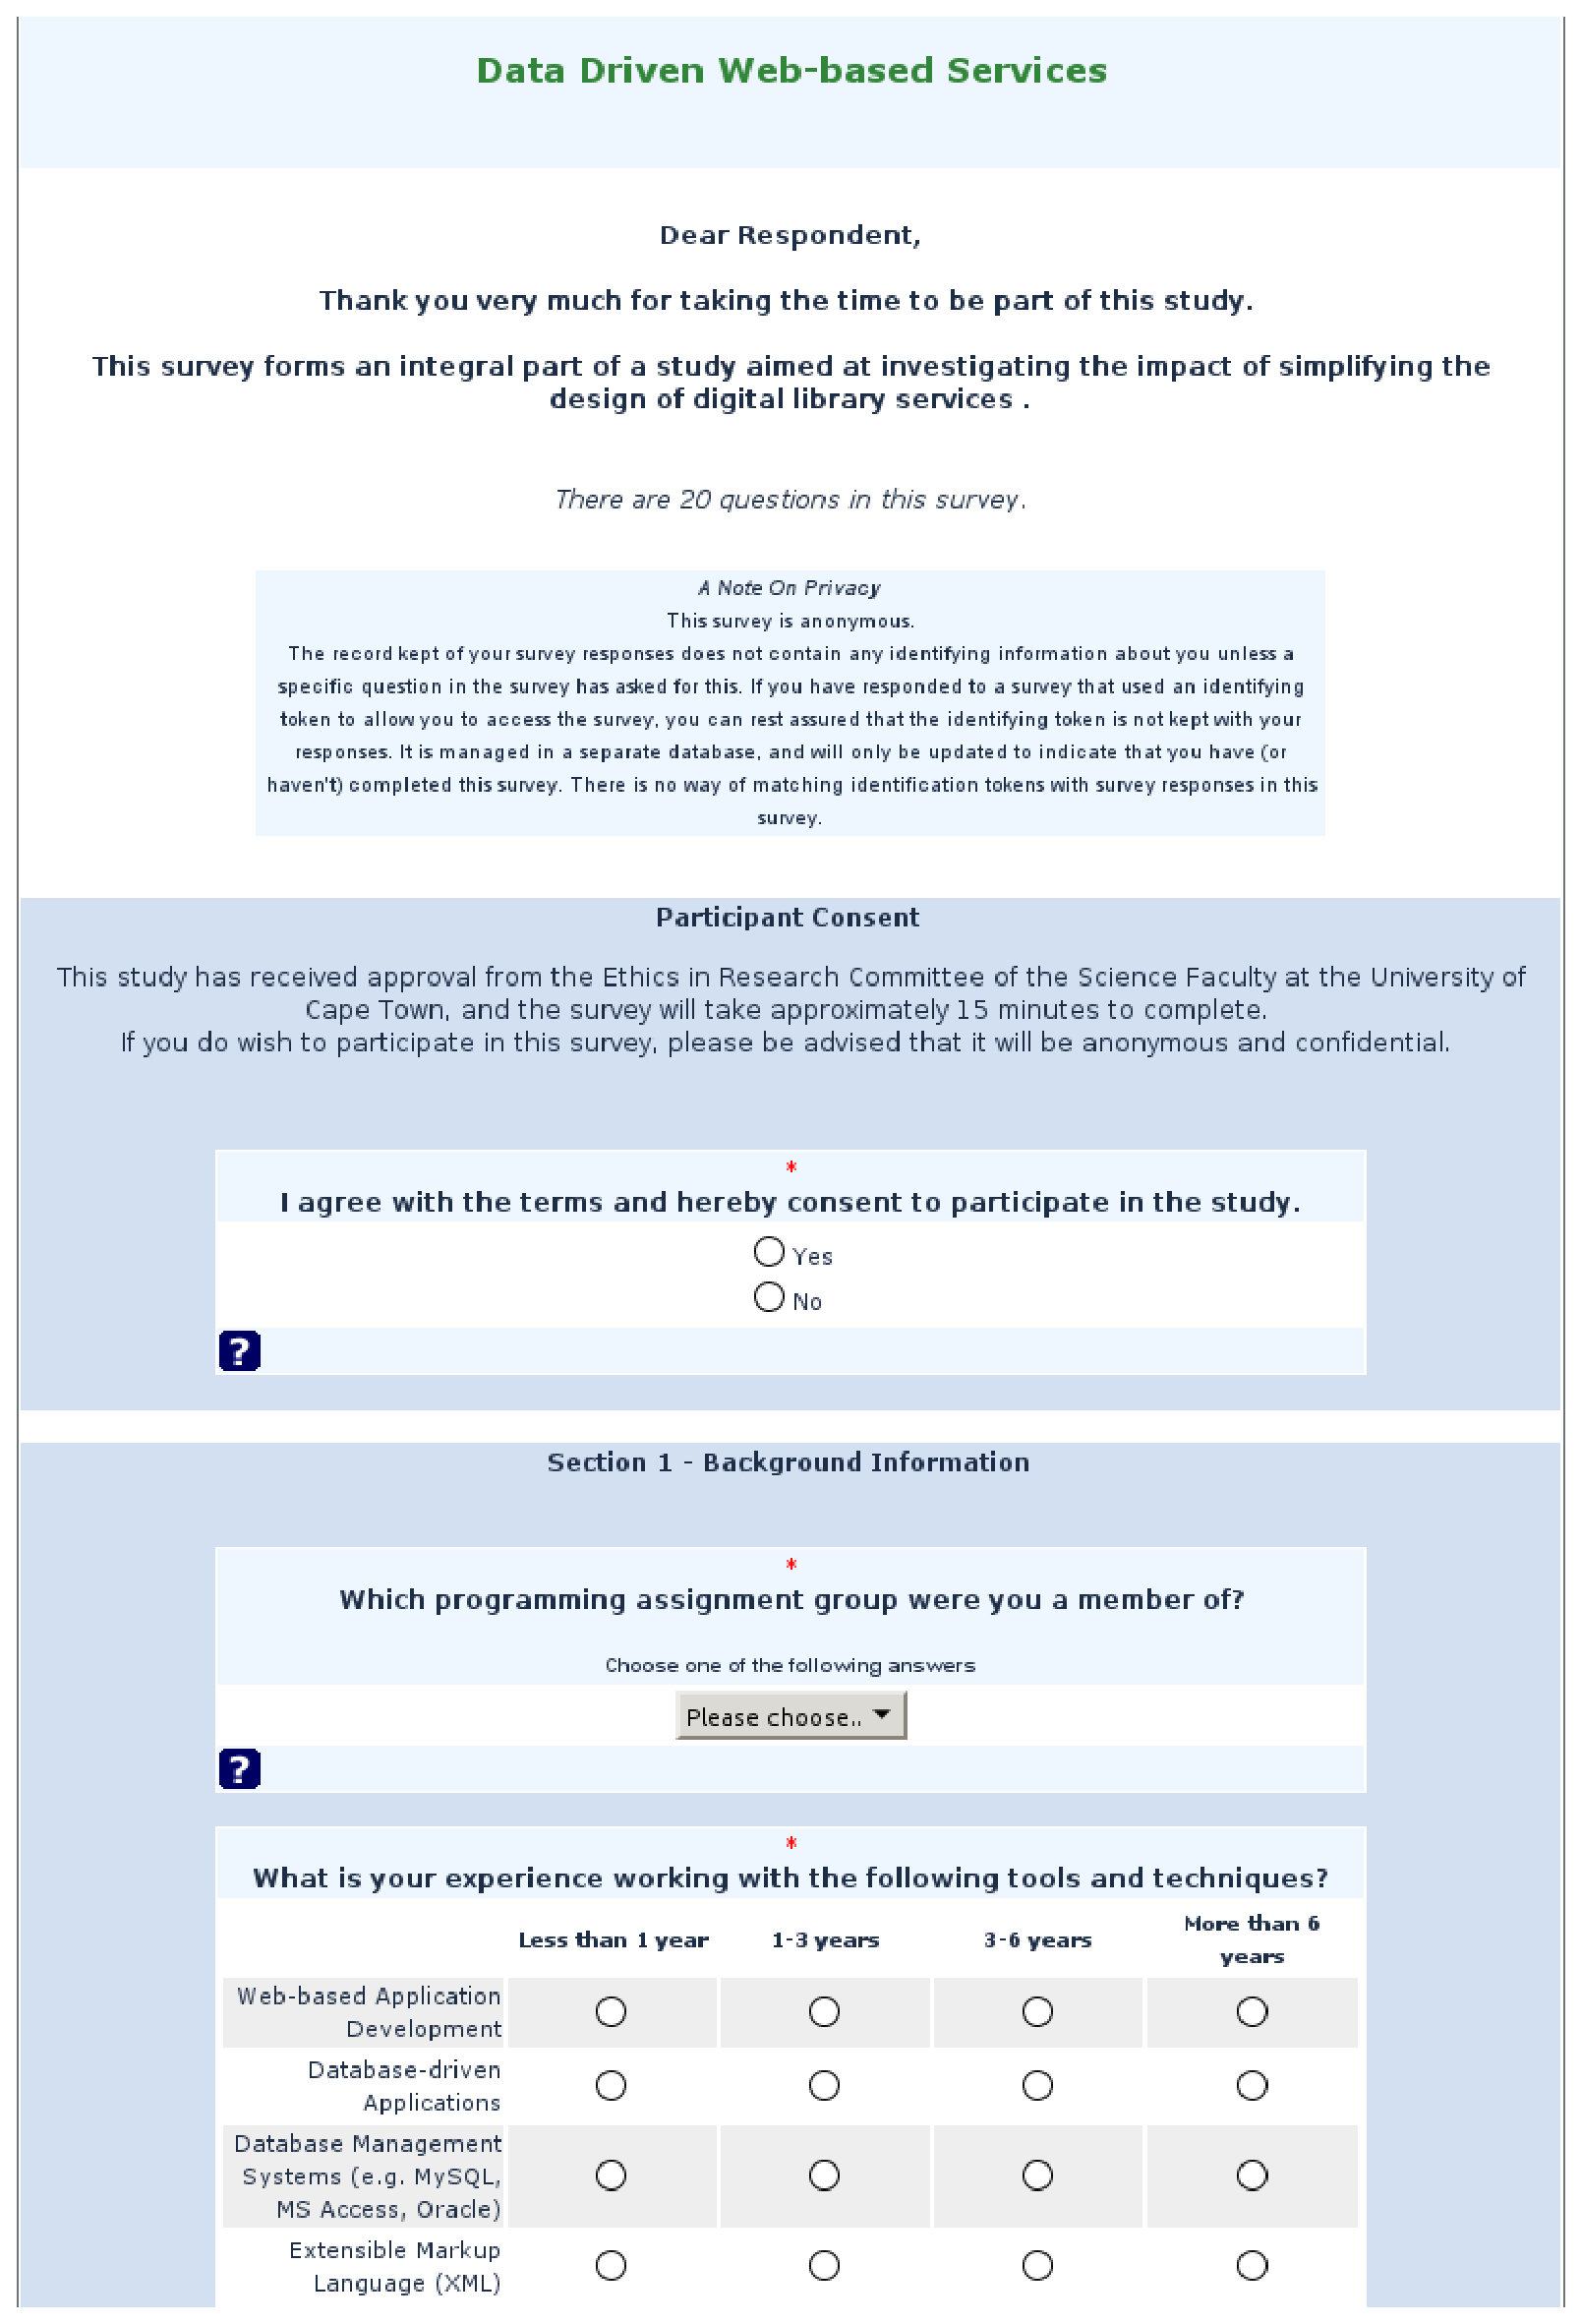
\includegraphics[width=0.95\textwidth]{appendicies/figures/developer-suvery-one-page-001.eps}
 }
 \caption[Screenshot of the online questionnaire (page 1 of 5)]{Screenshot of the online LimeSurvey questionnaire (page 1 of 5)}
 \label{appendix:appendicies:developer-suvery-one-page-001}
\end{subfigure}

\newpage

%\subsection{Section 1}
\begin{subfigure}[h]{\textwidth}
 \ContinuedFloat
 \centering
 %\subfloat[][]
 \framebox[\textwidth]{%
 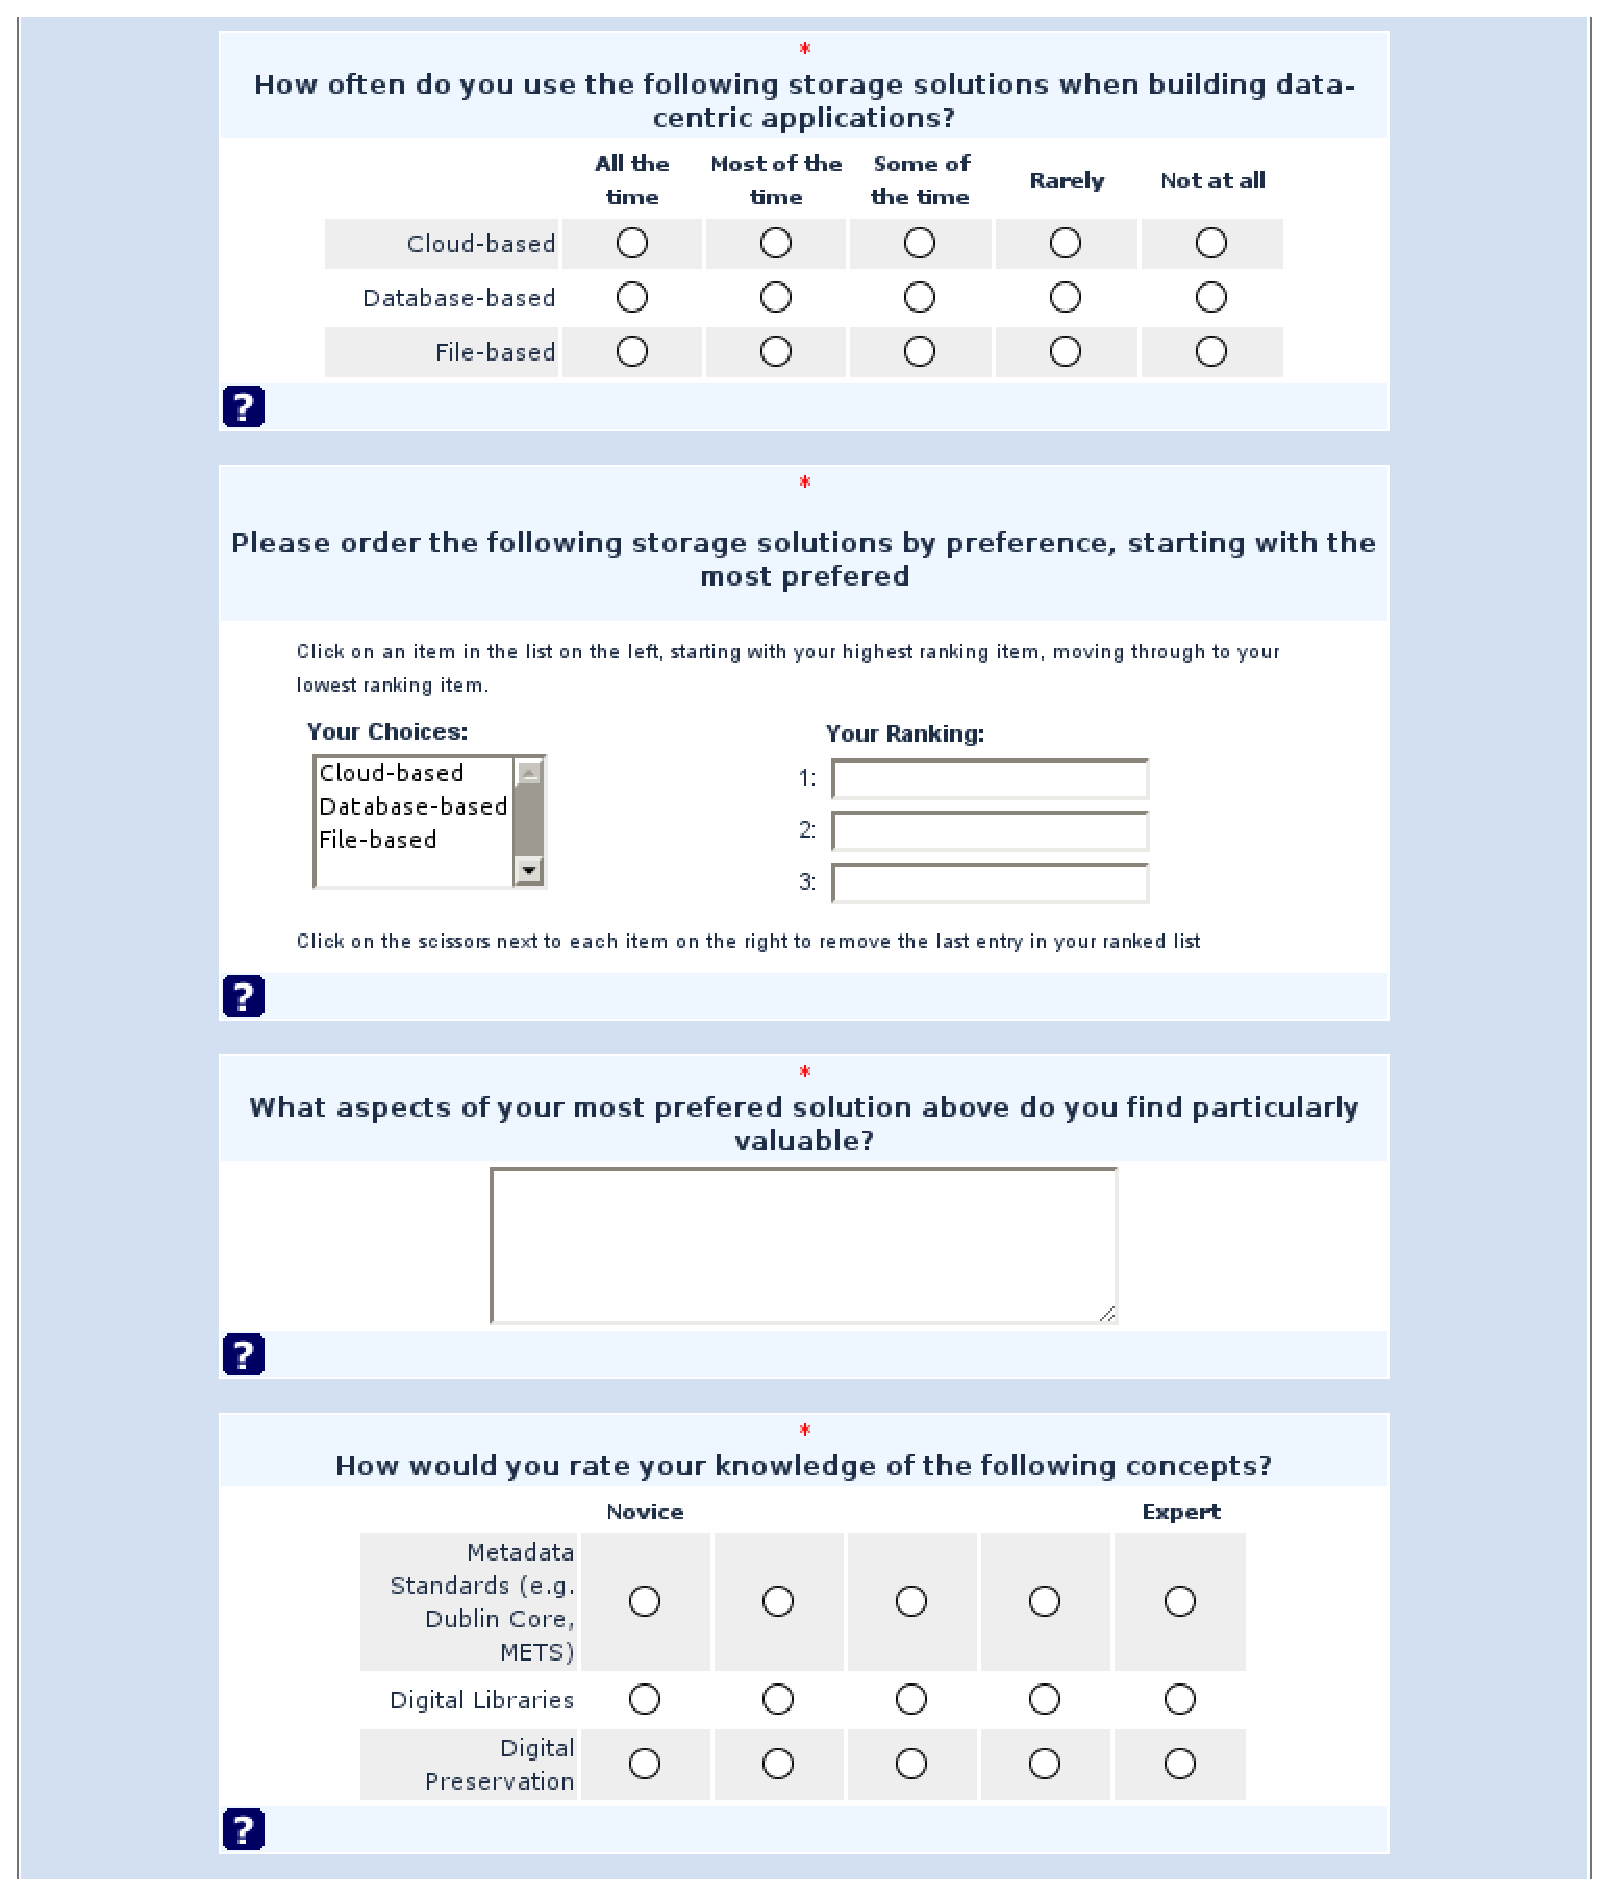
\includegraphics[width=0.95\textwidth]{appendicies/figures/developer-suvery-one-page-002.eps}
 }
 \caption[Screenshot of the online questionnaire (page 2 of 5)]{Screenshot of the online LimeSurvey questionnaire (page 2 of 5)}
 \label{appendix:appendicies:developer-suvery-one-page-002}
\end{subfigure}

\newpage

%\subsection{Section 1}
\begin{subfigure}[h]{\textwidth}
 \centering
 \framebox[\textwidth]{%
 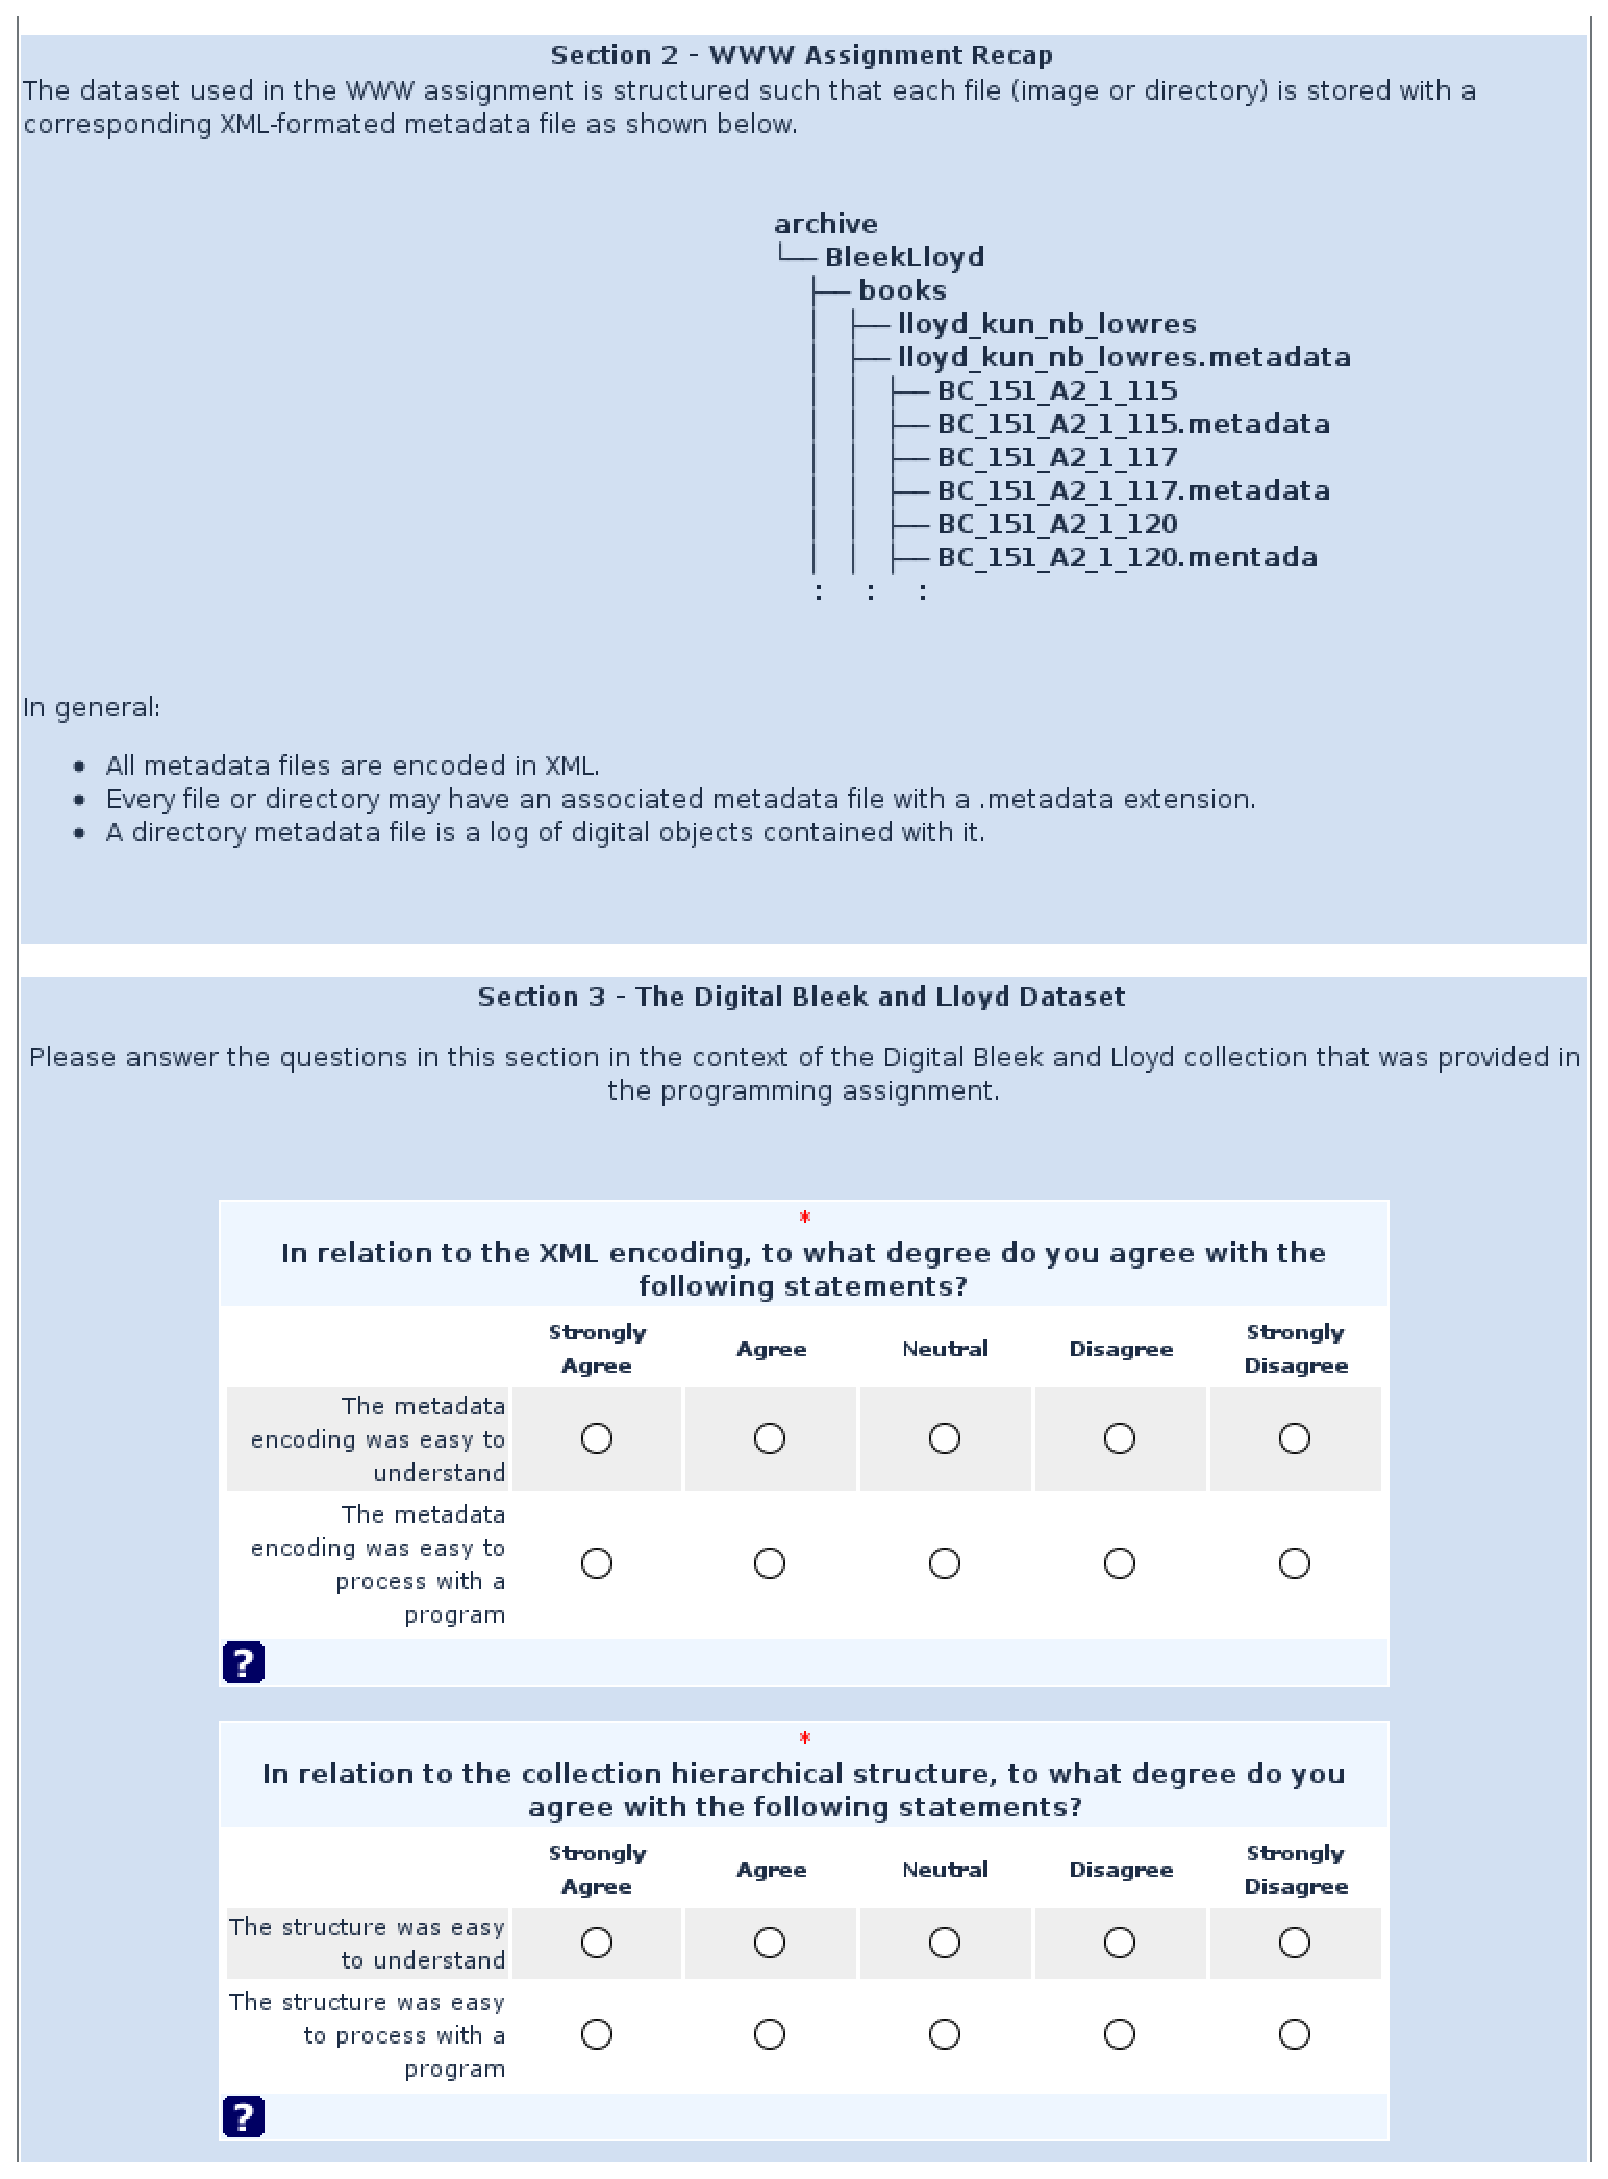
\includegraphics[width=0.95\textwidth]{appendicies/figures/developer-suvery-one-page-003.eps}
 }
 \caption[Screenshot of the online questionnaire (page 3 of 5)]{Screenshot of the online LimeSurvey questionnaire (page 3 of 5)}
 \label{appendix:appendicies:developer-suvery-one-page-003}
\end{subfigure}

\newpage

%\subsection{Section 1}
\begin{subfigure}[h]{\textwidth}
 \centering
 \framebox[\textwidth]{%
 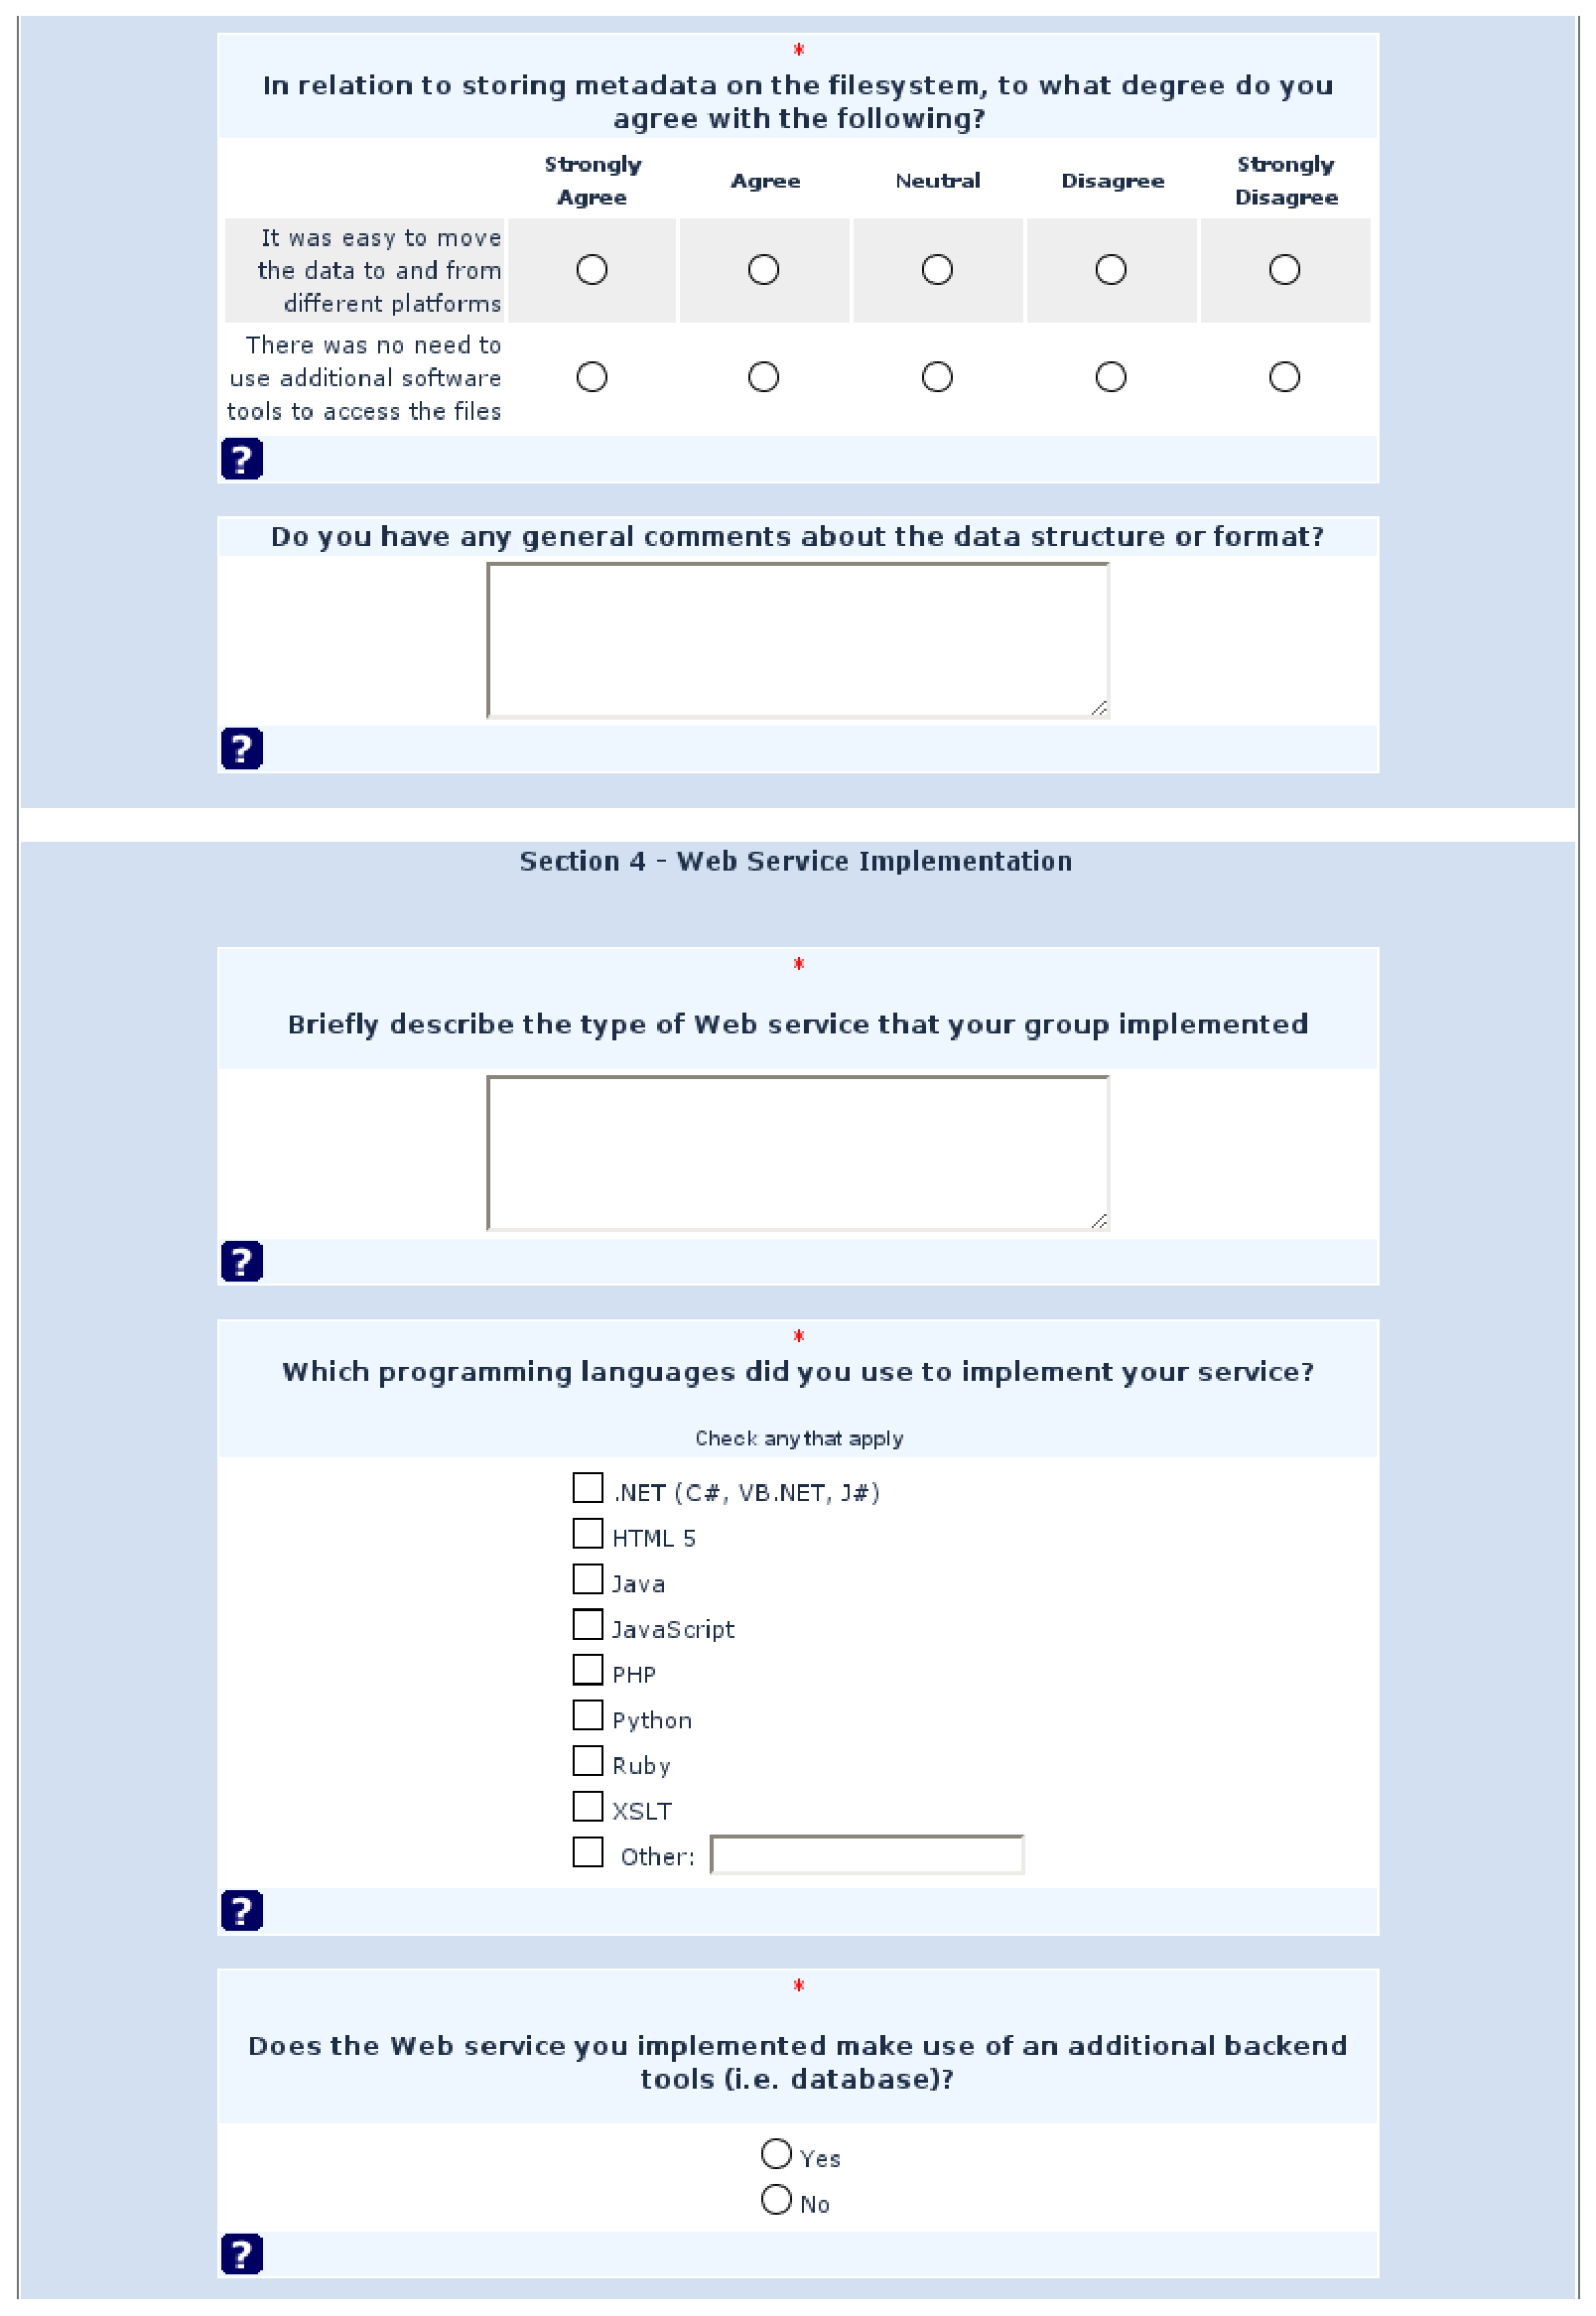
\includegraphics[width=0.95\textwidth]{appendicies/figures/developer-suvery-one-page-004.eps}
 }
 \caption[Screenshot of the online questionnaire (page 4 of 5)]{Screenshot of the online LimeSurvey questionnaire (page 4 of 5)}
 \label{appendix:appendicies:developer-suvery-one-page-004}
\end{subfigure}

\newpage

%\subsection{Section 1}
\begin{subfigure}[h]{\textwidth}
 \centering
 \framebox[\textwidth]{%
 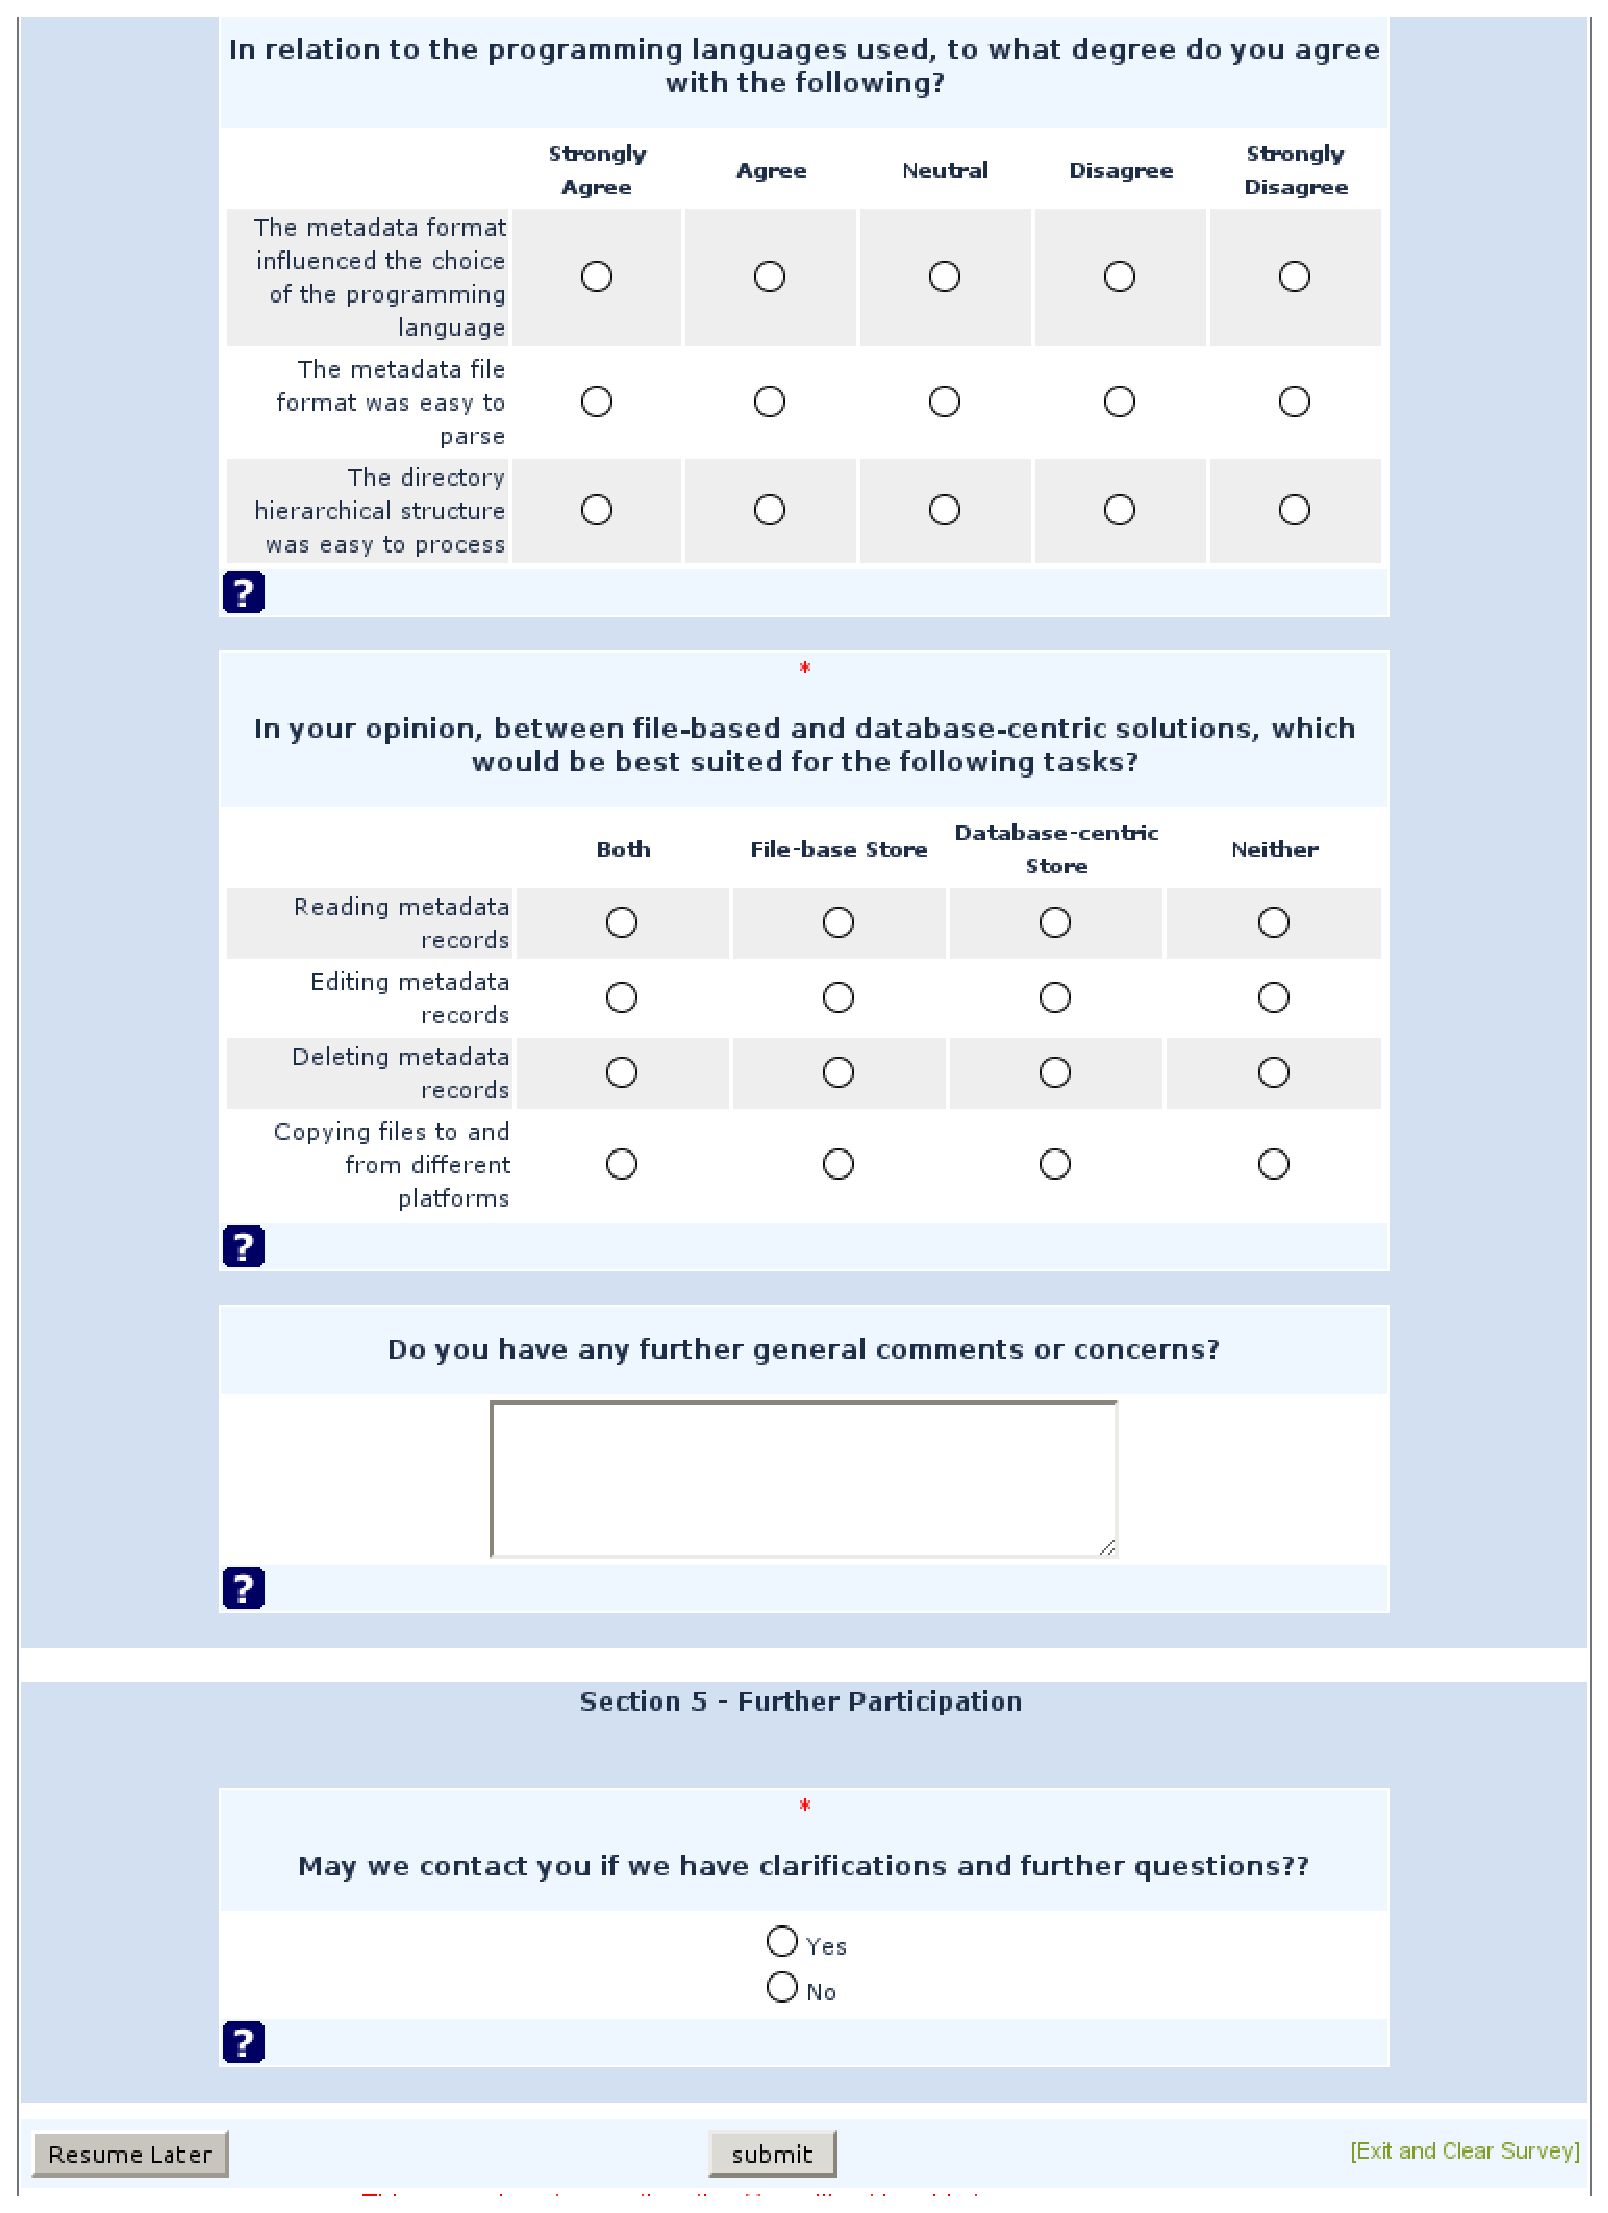
\includegraphics[width=0.95\textwidth]{appendicies/figures/developer-suvery-one-page-005.eps}
 }
 \caption[Screenshot of the online questionnaire (page 5 of 5)]{Screenshot of the online LimeSurvey questionnaire (page 5 of 5)}
 \label{appendix:appendicies:developer-suvery-one-page-005}
\end{subfigure}
 \caption[Screenshot of the online questionnaire]{Screenshot of the online LimeSurvey questionnaire}
 \label{appendix:appendicies:developer-suvery-all-in-one}
\end{figure}
\end{comment}
\chapter[Experiment raw data]{Experiment raw data\label{ch:appendex-d:experimentation}}

\tablespacing
\section[Developer survey]{Developer Survey results \label{ch:appendex-b:developer-survey:survey-results}}

\tablespacing
{\footnotesize
\begin{longtable}{
>{\arraybackslash}p{0.05\linewidth}|
>{\centering\arraybackslash}p{0.12\linewidth}|
>{\centering\arraybackslash}p{0.12\linewidth}|
>{\centering\arraybackslash}p{0.12\linewidth}|
>{\centering\arraybackslash}p{0.12\linewidth}|
>{\centering\arraybackslash}p{0.05\linewidth}}
 
\caption{Developer survey raw data for technologies background}
\label{tab:appendicies:survey:background:technologies}\\
 %%%\toprule
\hline
 %%%%%{} &
 \multicolumn{6}{c}{\textbf{Experience working with DL tools and techniques}}\\
 \cline{1-6}
 %%%\midrule
 %%%%%\hline
 \textbf{} &
 {\begin{sideways}\textbf{$<$ 1 year}\end{sideways}} &
 {\begin{sideways}\textbf{1-3 years}\end{sideways}} &
 {\begin{sideways}\textbf{3-6 years}\end{sideways}} &
 {\begin{sideways}\textbf{$>$ 6 years}\end{sideways}} &
 \textbf{} \\
 %%%\multicolumn{1}{c|}{\textbf{1}} &
 %%%\multicolumn{1}{c|}{\textbf{2}}&
 %%%\multicolumn{1}{c|}{\textbf{3}}&
 %%%\multicolumn{1}{c|}{\textbf{4}}&
 %%%\multicolumn{1}{c|}{\textbf{5}}\\
 %%%\midrule
 %%%%%\hline
 \endfirsthead
 
 \caption[]{(continued)}\\
 %%%\toprule
 \hline
%%%%%{} &
\multicolumn{6}{c}{\textbf{Experience working with DL tools and techniques}}\\
\cline{1-6}
%%%\midrule
%%%%%\hline
 \textbf{} &
 {\begin{sideways}\textbf{$<$ 1 year}\end{sideways}} &
 {\begin{sideways}\textbf{1-3 years}\end{sideways}} &
 {\begin{sideways}\textbf{3-6 years}\end{sideways}} &
 {\begin{sideways}\textbf{$>$ 6 years}\end{sideways}} &
 \textbf{} \\
 %%%\multicolumn{1}{c|}{\textbf{1}} &
 %%%\multicolumn{1}{c|}{\textbf{2}}&
 %%%\multicolumn{1}{c|}{\textbf{3}}&
 %%%\multicolumn{1}{c|}{\textbf{4}}&
 %%%\multicolumn{1}{c|}{\textbf{5}}\\
 %%%\midrule
 %%%%%\hline
 \endhead
 
 % Page footer
 %%%\midrule
 \hline
 \multicolumn{6}{r}{(Continued on next page)} \\
 \endfoot
 
 % Last page footer
 \bottomrule
 \endlastfoot
 
 %   &

 \cline{1-6} \multicolumn{1}{c}{\textbf{}} & \multicolumn{4}{c}{\textbf{[Database Management Systems]}} & {} \\ \cline{1-6}
{} & {5} & {19} & {1} & {1} & {} \\ \cline{2-6}
\cline{1-6} \multicolumn{1}{c}{\textbf{}} & \multicolumn{4}{c}{\textbf{[Database-Driven Applications]}} & {} \\ \cline{1-6}
{} & {13} & {11} & {1} & {1} & {} \\ \cline{2-6}
\cline{1-6} \multicolumn{1}{c}{\textbf{}} & \multicolumn{4}{c}{\textbf{[Extensible Markup Language]}} & {} \\ \cline{1-6}
{} & {12} & {13} & {1} & {0} & {}\\ \cline{2-6}
\cline{1-6} \multicolumn{1}{c}{\textbf{}} & \multicolumn{4}{c}{\textbf{[Web-Based Application Development]}} & {} \\ \cline{1-6}
{} & {14} & {10} & {1} & {1} & {} \\ \cline{2-6}

\end{longtable}
}
\bodyspacing

\tablespacing
{\footnotesize
\begin{longtable}{
>{\arraybackslash}p{0.05\linewidth}|
>{\centering\arraybackslash}p{0.09\linewidth}|
>{\centering\arraybackslash}p{0.09\linewidth}|
>{\centering\arraybackslash}p{0.09\linewidth}|
>{\centering\arraybackslash}p{0.09\linewidth}|
>{\centering\arraybackslash}p{0.09\linewidth}|
>{\centering\arraybackslash}p{0.05\linewidth}}
 
\caption{Developer survey raw data for DL concepts background}
\label{tab:appendicies:survey:background:dl-concepts}\\
 %%%\toprule
\hline
 %%%%%{} &
 \multicolumn{7}{c}{\textbf{Participants knowledge of DL concepts}}\\
 \cline{1-7}
 %%%\midrule
 {} & 
 {\begin{sideways}{Novice}\end{sideways}} &
 \multicolumn{3}{c|}{} &
 {\begin{sideways}{Expert}\end{sideways}} &
 {} \\
 \cline{1-7}
 %%%%%\hline
 \textbf{} &
 {\textbf{1}} &
 {\textbf{2}} &
 {\textbf{3}} &
 {\textbf{4}} &
 {\textbf{5}} &
 \textbf{} \\
 %%%\multicolumn{1}{c|}{\textbf{1}} &
 %%%\multicolumn{1}{c|}{\textbf{2}}&
 %%%\multicolumn{1}{c|}{\textbf{3}}&
 %%%\multicolumn{1}{c|}{\textbf{4}}&
 %%%\multicolumn{1}{c|}{\textbf{5}}\\
 %%%\midrule
 %%%%%\hline
 \endfirsthead
 
 \caption[]{(continued)}\\
 %%%\toprule
 \hline
%%%%%{} &
\multicolumn{7}{c}{\textbf{Participants knowledge of DL concepts}}\\
\cline{1-7}
%%%\midrule
 {} & 
 {\begin{sideways}{Novice}\end{sideways}} &
 \multicolumn{3}{c}{} &
 {\begin{sideways}{Expert}\end{sideways}} &
 {} \\
 \cline{1-7}
%%%%%\hline
 \textbf{} &
 {\textbf{1}} &
 {\textbf{2}} &
 {\textbf{3}} &
 {\textbf{4}} &
 {\textbf{5}} &
 \textbf{} \\
 %%%\multicolumn{1}{c|}{\textbf{1}} &
 %%%\multicolumn{1}{c|}{\textbf{2}}&
 %%%\multicolumn{1}{c|}{\textbf{3}}&
 %%%\multicolumn{1}{c|}{\textbf{4}}&
 %%%\multicolumn{1}{c|}{\textbf{5}}\\
 %%%\midrule
 %%%%%\hline
 \endhead
 
 % Page footer
 %%%\midrule
 \hline
 \multicolumn{7}{r}{(Continued on next page)} \\
 \endfoot
 
 % Last page footer
 \bottomrule
 \endlastfoot
 
 %   &

\cline{1-7} 
\multicolumn{1}{c}{\textbf{}} & \multicolumn{5}{c}{\textbf{[Digital Libraries]}} & {} \\ 
\cline{1-7}
{} & {10} & {11} & {5} & {0} & {0} & {} \\ 
\cline{1-7} 
\multicolumn{1}{c}{\textbf{}} & \multicolumn{5}{c}{\textbf{[Digital Preservation]}} & {} \\ 
\cline{1-7}
{} & {11} & {8} & {7} & {0} & {0} & {} \\ 
\cline{1-7} 
\multicolumn{1}{c}{\textbf{}} & \multicolumn{5}{c}{\textbf{[Metadata Standards]}} & {} \\ 
\cline{1-7}
{} & {8} & {9} & {8} & {1} & {0} & {} \\ 
\cline{1-7}

\end{longtable}
}
\bodyspacing

\tablespacing
{\footnotesize
\begin{longtable}{
>{\arraybackslash}p{0.05\linewidth}|
>{\centering\arraybackslash}p{0.09\linewidth}|
>{\centering\arraybackslash}p{0.09\linewidth}|
>{\centering\arraybackslash}p{0.09\linewidth}|
>{\centering\arraybackslash}p{0.09\linewidth}|
>{\centering\arraybackslash}p{0.09\linewidth}|
>{\centering\arraybackslash}p{0.05\linewidth}}
 
\caption{Developer survey raw data for storage usage frequencies}
\label{tab:appendicies:survey:background:storage-frequencies}\\
 %%%\toprule
\hline
 %%%%%{} &
 \multicolumn{7}{c}{\textbf{Storage solutions usage frequencies}}\\
 \cline{1-7}
 %%%\midrule
 %%%%%\hline
 \textbf{} &
 {\begin{sideways}\textbf{All the time}\end{sideways}} &
 {\begin{sideways}\textbf{Most times}\end{sideways}} &
 {\begin{sideways}\textbf{Not at all}\end{sideways}} &
 {\begin{sideways}\textbf{Rarely}\end{sideways}} &
 {\begin{sideways}\textbf{Some times}\end{sideways}} &
 \textbf{} \\
 %%%\multicolumn{1}{c|}{\textbf{1}} &
 %%%\multicolumn{1}{c|}{\textbf{2}}&
 %%%\multicolumn{1}{c|}{\textbf{3}}&
 %%%\multicolumn{1}{c|}{\textbf{4}}&
 %%%\multicolumn{1}{c|}{\textbf{5}}\\
 %%%\midrule
 %%%%%\hline
 \endfirsthead
 
 \caption[]{(continued)}\\
 %%%\toprule
 \hline
%%%%%{} &
\multicolumn{7}{c}{\textbf{Storage solutions usage frequencies}}\\
\cline{1-7}
%%%\midrule
%%%%%\hline
 \textbf{} &
 {\begin{sideways}\textbf{All the time}\end{sideways}} &
 {\begin{sideways}\textbf{Most times}\end{sideways}} &
 {\begin{sideways}\textbf{Not at all}\end{sideways}} &
 {\begin{sideways}\textbf{Rarely}\end{sideways}} &
 {\begin{sideways}\textbf{Some times}\end{sideways}} &
 \textbf{} \\
 %%%\multicolumn{1}{c|}{\textbf{1}} &
 %%%\multicolumn{1}{c|}{\textbf{2}}&
 %%%\multicolumn{1}{c|}{\textbf{3}}&
 %%%\multicolumn{1}{c|}{\textbf{4}}&
 %%%\multicolumn{1}{c|}{\textbf{5}}\\
 %%%\midrule
 %%%%%\hline
 \endhead
 
 % Page footer
 %%%\midrule
 \hline
 \multicolumn{7}{r}{(Continued on next page)} \\
 \endfoot
 
 % Last page footer
 \bottomrule
 \endlastfoot
 
 %   &

\cline{1-7} 
\multicolumn{1}{c}{\textbf{}} & \multicolumn{5}{c}{\textbf{ [Cloud-Based Solutions]}} & \multicolumn{1}{c}{} \\ 
\cline{1-7}
{} & {0} & {0} & {13} & {8} & {5} & {} \\ 
\cline{2-6}
\cline{1-7} 
\multicolumn{1}{c}{\textbf{}} & \multicolumn{5}{c}{\textbf{[Database-Based Solutions]}} & \multicolumn{1}{c}{} \\ 
\cline{1-7}
{} & {4} & {7} & {} & {5} & {10} & {} \\ 
\cline{2-6}
\cline{1-7} 
\multicolumn{1}{c}{\textbf{}} & \multicolumn{5}{c}{\textbf{[File-Based Solutions]}} & \multicolumn{1}{c}{} \\ 
\cline{1-7}
{} & {6} & {6} & {1} & {5} & {8} & {} \\ 
\cline{2-6}

\end{longtable}
}
\bodyspacing

\tablespacing
{\footnotesize
\begin{longtable}{
>{\arraybackslash}p{0.05\linewidth}|
>{\centering\arraybackslash}p{0.16\linewidth}|
>{\centering\arraybackslash}p{0.16\linewidth}|
>{\centering\arraybackslash}p{0.16\linewidth}|
>{\arraybackslash}p{0.05\linewidth}}
 
\caption{Developer survey raw data for storage rankings}
\label{tab:appendicies:survey:background:storage-rankings}\\
 %%%\toprule
\hline
 %%%%%{} &
 \multicolumn{5}{c}{\textbf{Storage solutions preferences}}\\
 \cline{1-5}
 %%%\midrule
 %%%%%\hline
 %%%%%\multicolumn{1}{c}{\textbf{}} &
 \textbf{} &
 {\begin{sideways}\textbf{Cloud}\end{sideways}} &
 {\begin{sideways}\textbf{Database}\end{sideways}} &
 {\begin{sideways}\textbf{File}\end{sideways}} &
 \textbf{} \\
 %%%%%\multicolumn{1}{c}{\textbf{}} \\
 %%%\multicolumn{1}{c|}{\textbf{1}} &
 %%%\multicolumn{1}{c|}{\textbf{2}}&
 %%%\multicolumn{1}{c|}{\textbf{3}}&
 %%%\multicolumn{1}{c|}{\textbf{4}}&
 %%%\multicolumn{1}{c|}{\textbf{5}}\\
 %%%\midrule
 %%%%%\hline
 \endfirsthead
 
 \caption[]{(continued)}\\
 %%%\toprule
 \hline
%%%%%{} &
\multicolumn{5}{c}{\textbf{Storage solutions preferences}}\\
\cline{1-5}
%%%\midrule
%%%%%\hline
%%%%%\multicolumn{1}{c}{\textbf{}} &
 \textbf{} &
 {\begin{sideways}\textbf{Cloud}\end{sideways}} &
 {\begin{sideways}\textbf{Database}\end{sideways}} &
 {\begin{sideways}\textbf{File}\end{sideways}} &
 \textbf{} \\
 %%%%%\multicolumn{1}{c}{\textbf{}} \\
 %%%\multicolumn{1}{c|}{\textbf{1}} &
 %%%\multicolumn{1}{c|}{\textbf{2}}&
 %%%\multicolumn{1}{c|}{\textbf{3}}&
 %%%\multicolumn{1}{c|}{\textbf{4}}&
 %%%\multicolumn{1}{c|}{\textbf{5}}\\
 %%%\midrule
 %%%%%\hline
 \endhead
 
 % Page footer
 %%%\midrule
 \hline
 \multicolumn{5}{r}{(Continued on next page)} \\
 \endfoot
 
 % Last page footer
 \bottomrule
 \endlastfoot
 
 %   &

\cline{1-5} \multicolumn{1}{c}{\textbf{}} & \multicolumn{3}{c}{\textbf{[Ranking 1]}} & {} \\ \cline{1-5}
{} & {8} & {12} & {6} & {} \\ \cline{2-4}
\cline{1-5} \multicolumn{1}{c}{\textbf{}} & \multicolumn{3}{c}{\textbf{[Ranking 2]}} & {} \\ \cline{1-5}
{} & {5} & {10} & {11} & {} \\ \cline{2-4}
\cline{1-5} \multicolumn{1}{c}{\textbf{}} & \multicolumn{3}{c}{\textbf{[Ranking 3]}} & {} \\ \cline{1-5}
{} & {13} & {4} & {9} & {} \\ \cline{1-5}
\multicolumn{1}{c}{} & \multicolumn{3}{c}{\textbf{Reasons for most prefered solution}} & {}\\
\cline{1-5}
 %%%%%\multicolumn{5}{p{0.60\textwidth}}{I understand databases better.} \\ \cline{1-5}
 %%%%%\multicolumn{5}{p{0.60\textwidth}}{Simple to set up and sheer control} \\ \cline{1-5}
 %%%%%\multicolumn{5}{p{0.60\textwidth}}{easy setup and connection to mysql database} \\ \cline{1-5}
 %%%%%\multicolumn{5}{p{0.60\textwidth}}{Remote access and the security of not having to manage your own hardware.} \\ \cline{1-5}
 %%%%%\multicolumn{5}{p{0.60\textwidth}}{Speed of accessing data, and its free.} \\ \cline{1-5}
 %%%%%\multicolumn{5}{p{0.60\textwidth}}{Backed up storage} \\ \cline{1-5}
 %%%%%\multicolumn{5}{p{0.60\textwidth}}{Ease of data manipulation and relations} \\ \cline{1-5}
 %%%%%\multicolumn{5}{p{0.60\textwidth}}{ease of access.} \\ \cline{1-5}
 %%%%%\multicolumn{5}{p{0.60\textwidth}}{File based is easyDatabase based is efficientCloud based is extensible} \\ \cline{1-5}
 %%%%%\multicolumn{5}{p{0.60\textwidth}}{Easy to query} \\ \cline{1-5}
 %%%%%\multicolumn{5}{p{0.60\textwidth}}{centralized management, easy of design, availability of support/literature} \\ \cline{1-5}
 %%%%%\multicolumn{5}{p{0.60\textwidth}}{the ability to sync all your data without the need for extensive hardware thus making it more convenient} \\ \cline{1-5}
 %%%%%\multicolumn{5}{p{0.60\textwidth}}{Fast parsing of data.} \\ \cline{1-5}
 %%%%%\multicolumn{5}{p{0.60\textwidth}}{Access anywhere and more scalable.} \\ \cline{1-5}
 %%%%%\multicolumn{5}{p{0.60\textwidth}}{offline access to resources} \\ \cline{1-5}
 %%%%%\multicolumn{5}{p{0.60\textwidth}}{Simple to implement and usually fufills all the requirements of data storage} \\ \cline{1-5}
 %%%%%\multicolumn{5}{p{0.60\textwidth}}{The existing infrastructure for storing and retrieving data} \\ \cline{1-5}
 %%%%%\multicolumn{5}{p{0.60\textwidth}}{file based} \\ \cline{1-5}
 %%%%%\multicolumn{5}{p{0.60\textwidth}}{conceptually easy to understand} \\ \cline{1-5}
 %%%%%\multicolumn{5}{p{0.60\textwidth}}{Quick access to files} \\ \cline{1-5}
 %%%%%\multicolumn{5}{p{0.60\textwidth}}{The fact that it is accessible from anywhere and can be used to keep data synced} \\ \cline{1-5}
 %%%%%\multicolumn{5}{p{0.60\textwidth}}{scalability and redundancy} \\ \cline{1-5}
 %%%%%\multicolumn{5}{p{0.60\textwidth}}{It\'s easy to access the data locally} \\ \cline{1-5}
 %%%%%\multicolumn{5}{p{0.60\textwidth}}{Cloud-based systems, as it is easier to access and has a lot of storage capacity.} \\ \cline{1-5}
 %%%%%\multicolumn{5}{p{0.60\textwidth}}{Querying a database table to retrieve a record is most useful for data.} \\ \cline{1-5}
 %%%%%\multicolumn{5}{p{0.60\textwidth}}{It stores data online, such that it won\'t be lost even if my host machine crashes} \\ \cline{1-5}

\end{longtable}
}
\bodyspacing

\tablespacing
{\footnotesize
\begin{longtable}{
>{\arraybackslash}p{0.05\linewidth}|
>{\centering\arraybackslash}p{0.09\linewidth}|
>{\centering\arraybackslash}p{0.09\linewidth}|
>{\centering\arraybackslash}p{0.09\linewidth}|
>{\centering\arraybackslash}p{0.09\linewidth}|
>{\centering\arraybackslash}p{0.09\linewidth}|
>{\centering\arraybackslash}p{0.05\linewidth}}
 
\caption{Developer survey raw data for repository structure}
\label{tab:appendicies:survey:background:repository-structure}\\
 %%%\toprule
\hline
 %%%%%{} &
 \multicolumn{7}{c}{\textbf{To what degree do you agree with the following}}\\
 \cline{1-7}
 %%%\midrule
 %%%%%\hline
 \textbf{} &
 {\begin{sideways}\textbf{Strong Agree}\end{sideways}} &
 {\begin{sideways}\textbf{Agree}\end{sideways}} &
 {\begin{sideways}\textbf{Neutral}\end{sideways}} &
 {\begin{sideways}\textbf{Disagree}\end{sideways}} &
 {\begin{sideways}\textbf{Strong Disagree}\end{sideways}} &
 \textbf{} \\
 %%%\multicolumn{1}{c|}{\textbf{1}} &
 %%%\multicolumn{1}{c|}{\textbf{2}}&
 %%%\multicolumn{1}{c|}{\textbf{3}}&
 %%%\multicolumn{1}{c|}{\textbf{4}}&
 %%%\multicolumn{1}{c|}{\textbf{5}}\\
 %%%\midrule
 %%%%%\hline
 \endfirsthead
 
 \caption[]{(continued)}\\
 %%%\toprule
 \hline
%%%%%{} &
\multicolumn{7}{c}{\textbf{To what degree do you agree with the following}}\\
\cline{1-7}
%%%\midrule
%%%%%\hline
 \textbf{} &
 {\begin{sideways}\textbf{Strong Agree}\end{sideways}} &
 {\begin{sideways}\textbf{Agree}\end{sideways}} &
 {\begin{sideways}\textbf{Neutral}\end{sideways}} &
 {\begin{sideways}\textbf{Disagree}\end{sideways}} &
 {\begin{sideways}\textbf{Strong Disagree}\end{sideways}} &
 \textbf{} \\
 %%%\multicolumn{1}{c|}{\textbf{1}} &
 %%%\multicolumn{1}{c|}{\textbf{2}}&
 %%%\multicolumn{1}{c|}{\textbf{3}}&
 %%%\multicolumn{1}{c|}{\textbf{4}}&
 %%%\multicolumn{1}{c|}{\textbf{5}}\\
 %%%\midrule
 %%%%%\hline
 \endhead
 
 % Page footer
 %%%\midrule
 \hline
 \multicolumn{7}{r}{(Continued on next page)} \\
 \endfoot
 
 % Last page footer
 \bottomrule
 \endlastfoot
 
 %   &

\cline{1-7} 
\multicolumn{1}{c}{\textbf{}} & \multicolumn{5}{c}{\textbf{[Easy to move the data]}} & {} \\ 
\cline{1-7}
{} & {3} & {15} & {6} & {2} & {0} & {} \\ 
\cline{1-7} 
\multicolumn{1}{c}{\textbf{}} & \multicolumn{5}{c}{\textbf{[No additional softwar required]}} & {} \\ 
\cline{1-7}
{} & {5} & {13} & {6} & {2} & {0} & {} \\ 
\cline{1-7}
\multicolumn{1}{c}{\textbf{}} & \multicolumn{5}{c}{\textbf{[Easy to process with program]}} & {} \\ 
\cline{1-7}
{} & {5} & {11} & {4} & {5} & {1} & {} \\ \cline{1-7}
\cline{1-7} 
\multicolumn{1}{c}{\textbf{}} & \multicolumn{5}{c}{\textbf{[Easy to understand]}} & {} \\ 
\cline{1-7}
{} & {2} & {10} & {8} & {6} & {0} & {} \\ 
\cline{1-7} 
\multicolumn{1}{c}{\textbf{}} & \multicolumn{5}{c}{\textbf{[XML was easy to process]}} & {} \\ 
\cline{1-7}
{} & {6} & {13} & {1} & {5} & {1} & {} \\ 
\cline{1-7}
\multicolumn{1}{c}{\textbf{}} & \multicolumn{5}{c}{\textbf{[XML was easy to understand]}} & {} \\ 
\cline{1-7}
{} & {4} & {12} & {7} & {3} & {0} & {} \\ 
\cline{1-7}

\end{longtable}
}
\bodyspacing

%
%

\tablespacing
{\footnotesize
\begin{longtable}{
>{\arraybackslash}p{0.05\linewidth}|
>{\centering\arraybackslash}p{0.12\linewidth}|
>{\centering\arraybackslash}p{0.12\linewidth}|
>{\centering\arraybackslash}p{0.12\linewidth}|
>{\centering\arraybackslash}p{0.12\linewidth}|
>{\centering\arraybackslash}p{0.05\linewidth}}
 
 \caption{Developer survey raw data for data management options}
\label{tab:appendicies:survey:data-management}\\
 %%%\toprule
\hline
 %%%%%{} &
 \multicolumn{6}{c}{\textbf{Solution best suited for data operations}}\\
 \cline{1-6}
 %%%\midrule
 %%%%%\hline
 \textbf{} &
 {\begin{sideways}\textbf{Both}\end{sideways}} &
 {\begin{sideways}\textbf{Database}\end{sideways}} &
 {\begin{sideways}\textbf{File Store}\end{sideways}} &
 {\begin{sideways}\textbf{Neither}\end{sideways}} &
 \textbf{} \\
 %%%\multicolumn{1}{c|}{\textbf{1}} &
 %%%\multicolumn{1}{c|}{\textbf{2}}&
 %%%\multicolumn{1}{c|}{\textbf{3}}&
 %%%\multicolumn{1}{c|}{\textbf{4}}&
 %%%\multicolumn{1}{c|}{\textbf{5}}\\
 %%%\midrule
 %%%%%\hline
 \endfirsthead
 
 \caption[]{(continued)}\\
 %%%\toprule
 \hline
%%%%%{} &
\multicolumn{6}{c}{\textbf{Solution best suited for data operations}}\\
\cline{1-6}
%%%\midrule
%%%%%\hline
 \textbf{} &
 {\begin{sideways}\textbf{Both}\end{sideways}} &
 {\begin{sideways}\textbf{Databasee}\end{sideways}} &
 {\begin{sideways}\textbf{File Store}\end{sideways}} &
 {\begin{sideways}\textbf{Neither}\end{sideways}} &
 \textbf{} \\
 %%%\multicolumn{1}{c|}{\textbf{1}} &
 %%%\multicolumn{1}{c|}{\textbf{2}}&
 %%%\multicolumn{1}{c|}{\textbf{3}}&
 %%%\multicolumn{1}{c|}{\textbf{4}}&
 %%%\multicolumn{1}{c|}{\textbf{5}}\\
 %%%\midrule
 %%%%%\hline
 \endhead
 
 % Page footer
 %%%\midrule
 \hline
 \multicolumn{6}{r}{(Continued on next page)} \\
 \endfoot
 
 % Last page footer
 \bottomrule
 \endlastfoot
 
 %   &

\cline{1-6} 
\multicolumn{1}{c}{\textbf{}} & \multicolumn{4}{c}{\textbf{[Copying files]}} & {} \\ 
\cline{1-6}
{} & {1} & {5} & {19} & {1} & {} \\ 
\cline{1-6}
\multicolumn{1}{c}{\textbf{}} & \multicolumn{4}{c}{\textbf{ [Deleting metadata records]}} & {} \\ 
\cline{1-6}
{} & {6} & {11} & {9} & {0} & {} \\ 
\cline{1-6} 
\multicolumn{1}{c}{\textbf{}} & \multicolumn{4}{c}{\textbf{ [Editing metadata records]}} & {} \\ 
\cline{1-6}
{} & {6} & {8} & {12} & {0} & {} \\ 
\cline{1-6}
\multicolumn{1}{c}{\textbf{}} & \multicolumn{4}{c}{\textbf{ [Reading metadata records]}} & {} \\ 
\cline{1-6}
{} & {5} & {7} & {13} & {1} & {} \\ 
\cline{1-6}

\end{longtable}
}
\bodyspacing

%
%

\tablespacing
{\footnotesize
\begin{longtable}{
>{\arraybackslash}p{0.05\linewidth}|
>{\centering\arraybackslash}p{0.075\linewidth}|
>{\centering\arraybackslash}p{0.075\linewidth}|
>{\centering\arraybackslash}p{0.075\linewidth}|
>{\centering\arraybackslash}p{0.075\linewidth}|
>{\centering\arraybackslash}p{0.075\linewidth}|
>{\centering\arraybackslash}p{0.075\linewidth}|
>{\centering\arraybackslash}p{0.05\linewidth}}
 
\caption{Developer survey raw data for programming languages}
\label{tab:appendicies:survey:programming-languages}\\
 %%%\toprule
\hline
 %%%%%{} &
 \multicolumn{8}{c}{\textbf{Programming languages used during in assignment}}\\
 \cline{1-8}
 %%%\midrule
 %%%%%\hline
 \textbf{} &
 {\begin{sideways}\textbf{C\#}\end{sideways}} &
 {\begin{sideways}\textbf{HTML5}\end{sideways}} &
 {\begin{sideways}\textbf{Java}\end{sideways}} &
 {\begin{sideways}\textbf{JavaScript}\end{sideways}} &
 {\begin{sideways}\textbf{PHP}\end{sideways}} &
 {\begin{sideways}\textbf{Python}\end{sideways}} &
 \textbf{} \\
 %%%\multicolumn{1}{c|}{\textbf{1}} &
 %%%\multicolumn{1}{c|}{\textbf{2}}&
 %%%\multicolumn{1}{c|}{\textbf{3}}&
 %%%\multicolumn{1}{c|}{\textbf{4}}&
 %%%\multicolumn{1}{c|}{\textbf{5}}\\
 %%%\midrule
 %%%%%\hline
 \endfirsthead
 
 \caption[]{(continued)}\\
 %%%\toprule
 \hline
%%%%%{} &
\multicolumn{8}{c}{\textbf{Programming languages used in assignment}}\\
\cline{1-8}
%%%\midrule
%%%%%\hline
 \textbf{} &
 {\begin{sideways}\textbf{C\#}\end{sideways}} &
 {\begin{sideways}\textbf{HTML5}\end{sideways}} &
 {\begin{sideways}\textbf{Java}\end{sideways}} &
 {\begin{sideways}\textbf{JavaScript}\end{sideways}} &
 {\begin{sideways}\textbf{PHP}\end{sideways}} &
 {\begin{sideways}\textbf{Python}\end{sideways}} &
 \textbf{} \\
 %%%\multicolumn{1}{c|}{\textbf{1}} &
 %%%\multicolumn{1}{c|}{\textbf{2}}&
 %%%\multicolumn{1}{c|}{\textbf{3}}&
 %%%\multicolumn{1}{c|}{\textbf{4}}&
 %%%\multicolumn{1}{c|}{\textbf{5}}\\
 %%%\midrule
 %%%%%\hline
 \endhead
 
 % Page footer
 %%%\midrule
 \hline
 \multicolumn{8}{r}{(Continued on next page)} \\
 \endfoot
 
 % Last page footer
 \bottomrule
 \endlastfoot
 
 %   &

 %%%%%\cline{1-8} 
 %%%%%{\textbf{}} & \multicolumn{6}{c}{\textbf{Which programming languages did you use to implement your service?}} & {} \\ 
 
 \cline{1-8}
 {} & {2} & {11} & {2} & {17} & {15} & {4} & {} \\ 
 \cline{1-8}

\end{longtable}
}
\bodyspacing

%
%

\tablespacing
{\footnotesize
\begin{longtable}{
>{\arraybackslash}p{0.05\linewidth}|
>{\centering\arraybackslash}p{0.28\linewidth}|
>{\centering\arraybackslash}p{0.28\linewidth}|
>{\centering\arraybackslash}p{0.05\linewidth}}
 
\caption{Developer survey raw data for additional backend tools}
\label{tab:appendicies:survey:additonal-backend-tools}\\
 %%%\toprule
\hline
 %%%%%{} &
 \multicolumn{4}{c}{\textbf{Additional backend tools used in assignment}}\\
 \cline{1-4}
 %%%\midrule
 %%%%%\hline
 \textbf{} &
 {\begin{sideways}\textbf{Yes}\end{sideways}} &
 {\begin{sideways}\textbf{No}\end{sideways}} &
 \textbf{} \\
 %%%\multicolumn{1}{c|}{\textbf{1}} &
 %%%\multicolumn{1}{c|}{\textbf{2}}&
 %%%\multicolumn{1}{c|}{\textbf{3}}&
 %%%\multicolumn{1}{c|}{\textbf{4}}&
 %%%\multicolumn{1}{c|}{\textbf{5}}\\
 %%%\midrule
 %%%%%\hline
 \endfirsthead
 
 \caption[]{(continued)}\\
 %%%\toprule
 \hline
%%%%%{} &
\multicolumn{4}{c}{\textbf{Additional backend tools used in assignment}}\\
\cline{1-4}
%%%\midrule
%%%%%\hline
 \textbf{} &
 {\begin{sideways}\textbf{Yes}\end{sideways}} &
 {\begin{sideways}\textbf{No}\end{sideways}} &
 \textbf{} \\
 %%%\multicolumn{1}{c|}{\textbf{1}} &
 %%%\multicolumn{1}{c|}{\textbf{2}}&
 %%%\multicolumn{1}{c|}{\textbf{3}}&
 %%%\multicolumn{1}{c|}{\textbf{4}}&
 %%%\multicolumn{1}{c|}{\textbf{5}}\\
 %%%\midrule
 %%%%%\hline
 \endhead
 
 % Page footer
 %%%\midrule
 \hline
 \multicolumn{4}{r}{(Continued on next page)} \\
 \endfoot
 
 % Last page footer
 \bottomrule
 \endlastfoot
 
 %   &

 %%%%%\cline{1-4} 
 %%%%%{\textbf{}} & \multicolumn{6}{c}{\textbf{Which programming languages did you use to implement your service?}} & {} \\ 
 
 \cline{1-4}
 {} & {11} & {15} & {} \\ \cline{1-4}
 \cline{1-4}

\end{longtable}
}
\bodyspacing

%
% question 11 in spreadsheet

\tablespacing
{\footnotesize
\begin{longtable}{
>{\arraybackslash}p{0.05\linewidth}|
>{\centering\arraybackslash}p{0.09\linewidth}|
>{\centering\arraybackslash}p{0.09\linewidth}|
>{\centering\arraybackslash}p{0.09\linewidth}|
>{\centering\arraybackslash}p{0.09\linewidth}|
>{\centering\arraybackslash}p{0.09\linewidth}|
>{\centering\arraybackslash}p{0.05\linewidth}}
 
 \caption{Developer survey raw data for programming languages}
\label{tab:appendicies:survey:background:repository-structure2}\\
 %%%\toprule
\hline
 %%%%%{} &
 \multicolumn{7}{c}{\textbf{To what degree do you agree with the following}}\\
 \cline{1-7}
 %%%\midrule
 %%%%%\hline
 \textbf{} &
 {\begin{sideways}\textbf{Strong Agree}\end{sideways}} &
 {\begin{sideways}\textbf{Agree}\end{sideways}} &
 {\begin{sideways}\textbf{Neutral}\end{sideways}} &
 {\begin{sideways}\textbf{Disagree}\end{sideways}} &
 {\begin{sideways}\textbf{Strong Disagree}\end{sideways}} &
 \textbf{} \\
 %%%\multicolumn{1}{c|}{\textbf{1}} &
 %%%\multicolumn{1}{c|}{\textbf{2}}&
 %%%\multicolumn{1}{c|}{\textbf{3}}&
 %%%\multicolumn{1}{c|}{\textbf{4}}&
 %%%\multicolumn{1}{c|}{\textbf{5}}\\
 %%%\midrule
 %%%%%\hline
 \endfirsthead
 
 \caption[]{(continued)}\\
 %%%\toprule
 \hline
%%%%%{} &
\multicolumn{7}{c}{\textbf{To what degree do you agree with the following}}\\
\cline{1-7}
%%%\midrule
%%%%%\hline
 \textbf{} &
 {\begin{sideways}\textbf{Strong Agree}\end{sideways}} &
 {\begin{sideways}\textbf{Agree}\end{sideways}} &
 {\begin{sideways}\textbf{Neutral}\end{sideways}} &
 {\begin{sideways}\textbf{Disagree}\end{sideways}} &
 {\begin{sideways}\textbf{Strong Disagree}\end{sideways}} &
 \textbf{} \\
 %%%\multicolumn{1}{c|}{\textbf{1}} &
 %%%\multicolumn{1}{c|}{\textbf{2}}&
 %%%\multicolumn{1}{c|}{\textbf{3}}&
 %%%\multicolumn{1}{c|}{\textbf{4}}&
 %%%\multicolumn{1}{c|}{\textbf{5}}\\
 %%%\midrule
 %%%%%\hline
 \endhead
 
 % Page footer
 %%%\midrule
 \hline
 \multicolumn{7}{r}{(Continued on next page)} \\
 \endfoot
 
 % Last page footer
 \bottomrule
 \endlastfoot
 
 %   &

\cline{1-7} 
\multicolumn{1}{c}{\textbf{}} & \multicolumn{5}{c}{\textbf{[structure was easy to process]}} & {} \\ 
\cline{1-7}
{} & {11} & {3} & {7} & {5} & {0} & {} \\ 
\cline{1-7} 
\multicolumn{1}{c}{\textbf{}} & \multicolumn{5}{c}{\textbf{[metadata was easy to parse]}} & {} \\ 
\cline{1-7}
{} & {16} & {5} & {3} & {2} & {0} & {} \\ 
\cline{1-7} 
\multicolumn{1}{c}{\textbf{}} & \multicolumn{5}{c}{\textbf{[metadata influenced language]}} & {} \\ 
\cline{1-7}
{} & {3} & {6} & {11} & {1} & {5} & {} \\ 
\cline{1-6}

\end{longtable}
}
\bodyspacing
\bodyspacing

\section[Performance benchmarks]{Performance benchmarks results}
\label{ch:appendicies:experiment-raw-data:performance-benchmarks}

\subsection[Workload]{Workload models}
\label{sec:appendex-d:workload-models}

\tablespacing
{\footnotesize
\begin{longtable}{
>{\arraybackslash}m{0.02\linewidth}|
>{\arraybackslash}m{0.07\linewidth}|
>{\centering\arraybackslash}m{0.13\linewidth}|
>{\centering\arraybackslash}m{0.13\linewidth}|
>{\centering\arraybackslash}m{0.13\linewidth}|
>{\centering\arraybackslash}m{0.13\linewidth}|
>{\centering\arraybackslash}m{0.13\linewidth}}
 
\caption{Performance experiment raw data for dataset models}
\label{tab:appendicies:performance:workload-design:dataset-models}\\
 %%%\toprule
\hline
 %%%%%{} &
 %%%%%\multicolumn{5}{c|}{\textbf{REPEATED RUNS}}\\
 %%%\midrule
 %%%%%\hline
 \textbf{} &
 \textbf{} &
 \textbf{Size} &
 \textbf{1} &
 \textbf{2} &
 \textbf{3} &
 \textbf{$\Sigma$} \\
 %%%\multicolumn{1}{c|}{\textbf{1}} &
 %%%\multicolumn{1}{c|}{\textbf{2}}&
 %%%\multicolumn{1}{c|}{\textbf{3}}&
 %%%\multicolumn{1}{c|}{\textbf{4}}&
 %%%\multicolumn{1}{c|}{\textbf{5}}\\
 %%%\midrule
 \hline
 \endfirsthead
 
 \caption[]{(continued)}\\
 %%%\toprule
 \hline
%%%%%{} &
%%%%%\multicolumn{5}{c|}{\textbf{REPEATED RUNS}}\\
%%%\midrule
%%%%%\hline
 \textbf{} &
 \textbf{} &
 \textbf{Size} &
 \textbf{1} &
 \textbf{2} &
 \textbf{3} &
 \textbf{$\Sigma$} \\
 %%%\multicolumn{1}{c|}{\textbf{1}} &
 %%%\multicolumn{1}{c|}{\textbf{2}}&
 %%%\multicolumn{1}{c|}{\textbf{3}}&
 %%%\multicolumn{1}{c|}{\textbf{4}}&
 %%%\multicolumn{1}{c|}{\textbf{5}}\\
 %%%\midrule
 \hline
 \endhead
 
 % Page footer
 %%%\midrule
 \hline
 \multicolumn{7}{r}{(Continued on next page)} \\
 \endfoot
 
 % Last page footer
 \bottomrule
 \endlastfoot
 
 %   &

 \cline{1-7} {\textbf{1}} & \multicolumn{6}{c}{\textbf{}} \\ \cline{1-7}
																       {} & \textbf{W1} & {\tablenum[table-format=4]{0.53}} & {\tablenum[table-format=4]{19}} & {{---}} & {{---}} & {\tablenum[table-format=4]{19}} \\ 
																       {} & \textbf{W2} & {\tablenum[table-format=4]{0.97}} & {\tablenum[table-format=4]{25}} & {{---}} & {{---}} & {\tablenum[table-format=4]{25}} \\ 
																       {} & \textbf{W3} & {\tablenum[table-format=4]{2}} & {\tablenum[table-format=4]{42}} & {{---}} & {{---}} & {\tablenum[table-format=4]{42}} \\ 
																       {} & \textbf{W4} & {\tablenum[table-format=4]{3.9}} & {\tablenum[table-format=4]{57}} & {{---}} & {{---}} & {\tablenum[table-format=4]{57}} \\ 
																       {} & \textbf{W5} & {\tablenum[table-format=4]{7.6}} & {\tablenum[table-format=4]{67}} & {{---}} & {{---}} & {\tablenum[table-format=4]{67}} \\ 
																       {} & \textbf{W6} & {\tablenum[table-format=4]{15}} & {\tablenum[table-format=4]{83}} & {{---}} & {{---}} & {\tablenum[table-format=4]{83}} \\ 
																       {} & \textbf{W7} & {\tablenum[table-format=4]{30}} & {\tablenum[table-format=4]{100}} & {{---}} & {{---}} & {\tablenum[table-format=4]{100}} \\ 
																       {} & \textbf{W8} & {\tablenum[table-format=4]{60}} & {\tablenum[table-format=4]{112}} & {{---}} & {{---}} & {\tablenum[table-format=4]{112}} \\ 
																       {} & \textbf{W9} & {\tablenum[table-format=4]{118}} & {\tablenum[table-format=4]{116}} & {{---}} & {{---}} & {\tablenum[table-format=4]{116}} \\ 
																       {} & \textbf{W10} & {\tablenum[table-format=4]{236}} & {\tablenum[table-format=4]{119}} & {{---}} & {{---}} & {\tablenum[table-format=4]{119}} \\ 
																       {} & \textbf{W11} & {\tablenum[table-format=4]{471}} & {\tablenum[table-format=4]{127}} & {{---}} & {{---}} & {\tablenum[table-format=4]{127}} \\ 
																       {} & \textbf{W12} & {\tablenum[table-format=4]{942}} & {\tablenum[table-format=4]{129}} & {{---}} & {{---}} & {\tablenum[table-format=4]{129}} \\ 
																       {} & \textbf{W13} & {\tablenum[table-format=4]{1945.6}} & {\tablenum[table-format=4]{128}} & {{---}} & {{---}} & {\tablenum[table-format=4]{128}} \\ 
																       {} & \textbf{W14} & {\tablenum[table-format=4]{3788.8}} & {\tablenum[table-format=4]{131}} & {{---}} & {{---}} & {\tablenum[table-format=4]{131}} \\ 
																       {} & \textbf{W15} & {\tablenum[table-format=4]{7577.6}} & {\tablenum[table-format=4]{131}} & {{---}} & {{---}} & {\tablenum[table-format=4]{131}} \\ 
 \cline{1-7} {\textbf{2}} & \multicolumn{6}{c}{\textbf{}} \\ \cline{1-7}
																       {} & \textbf{W1} & {\tablenum[table-format=4]{0.78}} & {\tablenum[table-format=4]{19}} & {\tablenum[table-format=4]{66}} & {{---}} & {\tablenum[table-format=4]{85}} \\ 
																       {} & \textbf{W2} & {\tablenum[table-format=4]{1.4}} & {\tablenum[table-format=4]{25}} & {\tablenum[table-format=4]{105}} & {{---}} & {\tablenum[table-format=4]{130}} \\ 
																       {} & \textbf{W3} & {\tablenum[table-format=4]{2.7}} & {\tablenum[table-format=4]{42}} & {\tablenum[table-format=4]{186}} & {{---}} & {\tablenum[table-format=4]{228}} \\ 
																       {} & \textbf{W4} & {\tablenum[table-format=4]{4.9}} & {\tablenum[table-format=4]{57}} & {\tablenum[table-format=4]{264}} & {{---}} & {\tablenum[table-format=4]{321}} \\ 
																       {} & \textbf{W5} & {\tablenum[table-format=4]{9.2}} & {\tablenum[table-format=4]{67}} & {\tablenum[table-format=4]{420}} & {{---}} & {\tablenum[table-format=4]{487}} \\ 
																       {} & \textbf{W6} & {\tablenum[table-format=4]{17}} & {\tablenum[table-format=4]{83}} & {\tablenum[table-format=4]{551}} & {{---}} & {\tablenum[table-format=4]{634}} \\ 
																       {} & \textbf{W7} & {\tablenum[table-format=4]{33}} & {\tablenum[table-format=4]{100}} & {\tablenum[table-format=4]{771}} & {{---}} & {\tablenum[table-format=4]{871}} \\ 
																       {} & \textbf{W8} & {\tablenum[table-format=4]{64}} & {\tablenum[table-format=4]{112}} & {\tablenum[table-format=4]{1071}} & {{---}} & {\tablenum[table-format=4]{1183}} \\ 
																       {} & \textbf{W9} & {\tablenum[table-format=4]{123}} & {\tablenum[table-format=4]{116}} & {\tablenum[table-format=4]{1314}} & {{---}} & {\tablenum[table-format=4]{1430}} \\ 
																       {} & \textbf{W10} & {\tablenum[table-format=4]{243}} & {\tablenum[table-format=4]{119}} & {\tablenum[table-format=4]{1687}} & {\tablenum[table-format=4]{1}} & {\tablenum[table-format=4]{1807}} \\ 
																       {} & \textbf{W11} & {\tablenum[table-format=4]{481}} & {\tablenum[table-format=4]{127}} & {\tablenum[table-format=4]{2058}} & {{---}} & {\tablenum[table-format=4]{2185}} \\ 
																       {} & \textbf{W12} & {\tablenum[table-format=4]{957}} & {\tablenum[table-format=4]{129}} & {\tablenum[table-format=4]{2400}} & {{---}} & {\tablenum[table-format=4]{2529}} \\ 
																       {} & \textbf{W13} & {\tablenum[table-format=4]{1945.6}} & {\tablenum[table-format=4]{128}} & {\tablenum[table-format=4]{2747}} & {{---}} & {\tablenum[table-format=4]{2875}} \\ 
																       {} & \textbf{W14} & {\tablenum[table-format=4]{3891.2}} & {\tablenum[table-format=4]{131}} & {\tablenum[table-format=4]{3093}} & {\tablenum[table-format=4]{1}} & {\tablenum[table-format=4]{3225}} \\ 
																       {} & \textbf{W15} & {\tablenum[table-format=4]{7680}} & {\tablenum[table-format=4]{131}} & {\tablenum[table-format=4]{3457}} & {\tablenum[table-format=4]{1}} & {\tablenum[table-format=4]{3589}} \\ 
 \cline{1-7} {\textbf{3}} & \multicolumn{6}{c}{\textbf{}} \\ \cline{1-7}
																       {} & \textbf{W1} & {\tablenum[table-format=4]{1.2}} & {\tablenum[table-format=4]{19}} & {\tablenum[table-format=4]{66}} & {\tablenum[table-format=4]{96}} & {\tablenum[table-format=4]{181}} \\ 
																       {} & \textbf{W2} & {\tablenum[table-format=4]{2.1}} & {\tablenum[table-format=4]{25}} & {\tablenum[table-format=4]{105}} & {\tablenum[table-format=4]{174}} & {\tablenum[table-format=4]{304}} \\ 
																       {} & \textbf{W3} & {\tablenum[table-format=4]{4}} & {\tablenum[table-format=4]{42}} & {\tablenum[table-format=4]{186}} & {\tablenum[table-format=4]{331}} & {\tablenum[table-format=4]{559}} \\ 
																       {} & \textbf{W4} & {\tablenum[table-format=4]{7.2}} & {\tablenum[table-format=4]{57}} & {\tablenum[table-format=4]{264}} & {\tablenum[table-format=4]{585}} & {\tablenum[table-format=4]{906}} \\ 
																       {} & \textbf{W5} & {\tablenum[table-format=4]{14}} & {\tablenum[table-format=4]{67}} & {\tablenum[table-format=4]{420}} & {\tablenum[table-format=4]{1035}} & {\tablenum[table-format=4]{1522}} \\ 
																       {} & \textbf{W6} & {\tablenum[table-format=4]{24}} & {\tablenum[table-format=4]{83}} & {\tablenum[table-format=4]{551}} & {\tablenum[table-format=4]{1736}} & {\tablenum[table-format=4]{2370}} \\ 
																       {} & \textbf{W7} & {\tablenum[table-format=4]{44}} & {\tablenum[table-format=4]{100}} & {\tablenum[table-format=4]{771}} & {\tablenum[table-format=4]{2854}} & {\tablenum[table-format=4]{3725}} \\ 
																       {} & \textbf{W8} & {\tablenum[table-format=4]{80}} & {\tablenum[table-format=4]{112}} & {\tablenum[table-format=4]{1071}} & {\tablenum[table-format=4]{4499}} & {\tablenum[table-format=4]{5682}} \\ 
																       {} & \textbf{W9} & {\tablenum[table-format=4]{147}} & {\tablenum[table-format=4]{116}} & {\tablenum[table-format=4]{1314}} & {\tablenum[table-format=4]{6612}} & {\tablenum[table-format=4]{8042}} \\ 
																       {} & \textbf{W10} & {\tablenum[table-format=4]{277}} & {\tablenum[table-format=4]{119}} & {\tablenum[table-format=4]{1687}} & {\tablenum[table-format=4]{9689}} & {\tablenum[table-format=4]{11495}} \\ 
																       {} & \textbf{W11} & {\tablenum[table-format=4]{526}} & {\tablenum[table-format=4]{127}} & {\tablenum[table-format=4]{2059}} & {\tablenum[table-format=4]{13335}} & {\tablenum[table-format=4]{15521}} \\ 
																       {} & \textbf{W12} & {\tablenum[table-format=4]{1016}} & {\tablenum[table-format=4]{129}} & {\tablenum[table-format=4]{2401}} & {\tablenum[table-format=4]{18012}} & {\tablenum[table-format=4]{20542}} \\ 
																       {} & \textbf{W13} & {\tablenum[table-format=4]{2048}} & {\tablenum[table-format=4]{128}} & {\tablenum[table-format=4]{2748}} & {\tablenum[table-format=4]{23664}} & {\tablenum[table-format=4]{26540}} \\ 
																       {} & \textbf{W14} & {\tablenum[table-format=4]{3993.6}} & {\tablenum[table-format=4]{131}} & {\tablenum[table-format=4]{3094}} & {\tablenum[table-format=4]{30177}} & {\tablenum[table-format=4]{33402}} \\ 
																       {} & \textbf{W15} & {\tablenum[table-format=4]{7782.4}} & {\tablenum[table-format=4]{131}} & {\tablenum[table-format=4]{3460}} & {\tablenum[table-format=4]{37357}} & {\tablenum[table-format=4]{40948}} \\ 

\end{longtable}
}
\bodyspacing

\subsection[Ingestion]{Ingestion}
\label{sec:appendex-d:ingestion}

\tablespacing
{\footnotesize
\begin{longtable}{
>{\arraybackslash}m{0.02\linewidth}|
>{\arraybackslash}m{0.07\linewidth}|
>{\centering\arraybackslash}m{0.13\linewidth}|
>{\centering\arraybackslash}m{0.13\linewidth}|
>{\centering\arraybackslash}m{0.13\linewidth}|
>{\centering\arraybackslash}m{0.13\linewidth}|
>{\centering\arraybackslash}m{0.13\linewidth}}
 
 \caption{Performance experiment raw data for ingestion}
\label{tab:appendicies:performance:ingest:levels}\\
 %%%\toprule
\hline
 %%%%%{} &
 %%%%%\multicolumn{5}{c|}{\textbf{REPEATED RUNS}}\\
 %%%\midrule
 %%%%%\hline
 \textbf{} &
 \textbf{} &
 \textbf{1} &
 \textbf{2} &
 \textbf{3} &
 \textbf{4} &
 \textbf{5} \\
 %%%\multicolumn{1}{c|}{\textbf{1}} &
 %%%\multicolumn{1}{c|}{\textbf{2}}&
 %%%\multicolumn{1}{c|}{\textbf{3}}&
 %%%\multicolumn{1}{c|}{\textbf{4}}&
 %%%\multicolumn{1}{c|}{\textbf{5}}\\
 %%%\midrule
 \hline
 \endfirsthead
 
 \caption[]{(continued)}\\
 %%%\toprule
 \hline
%%%%%{} &
%%%%%\multicolumn{5}{c|}{\textbf{REPEATED RUNS}}\\
%%%\midrule
%%%%%\hline
 \textbf{} &
 \textbf{} &
 \textbf{1} &
 \textbf{2} &
 \textbf{3} &
 \textbf{4} &
 \textbf{5} \\
 %%%\multicolumn{1}{c|}{\textbf{1}} &
 %%%\multicolumn{1}{c|}{\textbf{2}}&
 %%%\multicolumn{1}{c|}{\textbf{3}}&
 %%%\multicolumn{1}{c|}{\textbf{4}}&
 %%%\multicolumn{1}{c|}{\textbf{5}}\\
 %%%\midrule
 \hline
 \endhead
 
 % Page footer
 %%%\midrule
 \hline
 \multicolumn{7}{r}{(Continued on next page)} \\
 \endfoot
 
 % Last page footer
 \bottomrule
 \endlastfoot
 
 %   &

\cline{1-7} {\textbf{1}} & \multicolumn{6}{c}{\textbf{Phase = Overall}} \\ \cline{1-7}
															       {} & \textbf{W1} & {\tablenum[table-format=4]{289.64}} & {\tablenum[table-format=4]{2.83}} & {\tablenum[table-format=4]{10.29}} & {\tablenum[table-format=4]{2.76}} & {\tablenum[table-format=4]{3.28}} \\ 
															       {} & \textbf{W2} & {\tablenum[table-format=4]{53.66}} & {\tablenum[table-format=4]{2.79}} & {\tablenum[table-format=4]{2.91}} & {\tablenum[table-format=4]{14.28}} & {\tablenum[table-format=4]{2.8}} \\ 
															       {} & \textbf{W3} & {\tablenum[table-format=4]{47.44}} & {\tablenum[table-format=4]{2.77}} & {\tablenum[table-format=4]{2.77}} & {\tablenum[table-format=4]{2.84}} & {\tablenum[table-format=4]{2.77}} \\ 
															       {} & \textbf{W4} & {\tablenum[table-format=4]{34.32}} & {\tablenum[table-format=4]{2.77}} & {\tablenum[table-format=4]{2.76}} & {\tablenum[table-format=4]{2.79}} & {\tablenum[table-format=4]{2.81}} \\ 
															       {} & \textbf{W5} & {\tablenum[table-format=4]{27.63}} & {\tablenum[table-format=4]{2.79}} & {\tablenum[table-format=4]{2.92}} & {\tablenum[table-format=4]{2.78}} & {\tablenum[table-format=4]{2.87}} \\ 
															       {} & \textbf{W6} & {\tablenum[table-format=4]{1418.27}} & {\tablenum[table-format=4]{2.76}} & {\tablenum[table-format=4]{2.78}} & {\tablenum[table-format=4]{2.8}} & {\tablenum[table-format=4]{2.76}} \\ 
															       {} & \textbf{W7} & {\tablenum[table-format=4]{48.34}} & {\tablenum[table-format=4]{4.52}} & {\tablenum[table-format=4]{2.9}} & {\tablenum[table-format=4]{2.92}} & {\tablenum[table-format=4]{2.99}} \\ 
															       {} & \textbf{W8} & {\tablenum[table-format=4]{60.58}} & {\tablenum[table-format=4]{2.78}} & {\tablenum[table-format=4]{2.8}} & {\tablenum[table-format=4]{2.76}} & {\tablenum[table-format=4]{2.85}} \\ 
															       {} & \textbf{W9} & {\tablenum[table-format=4]{76.6}} & {\tablenum[table-format=4]{2.78}} & {\tablenum[table-format=4]{2.78}} & {\tablenum[table-format=4]{2.76}} & {\tablenum[table-format=4]{2.86}} \\ 
															       {} & \textbf{W10} & {\tablenum[table-format=4]{247.31}} & {\tablenum[table-format=4]{2.99}} & {\tablenum[table-format=4]{2.84}} & {\tablenum[table-format=4]{2.87}} & {\tablenum[table-format=4]{2.85}} \\ 
															       {} & \textbf{W11} & {\tablenum[table-format=4]{41.79}} & {\tablenum[table-format=4]{2.97}} & {\tablenum[table-format=4]{3.05}} & {\tablenum[table-format=4]{3}} & {\tablenum[table-format=4]{2.8}} \\ 
															       {} & \textbf{W12} & {\tablenum[table-format=4]{64.93}} & {\tablenum[table-format=4]{2.9}} & {\tablenum[table-format=4]{5.5}} & {\tablenum[table-format=4]{4.53}} & {\tablenum[table-format=4]{2.86}} \\ 
															       {} & \textbf{W13} & {\tablenum[table-format=4]{52.42}} & {\tablenum[table-format=4]{3.04}} & {\tablenum[table-format=4]{3.08}} & {\tablenum[table-format=4]{2.77}} & {\tablenum[table-format=4]{2.77}} \\ 
															       {} & \textbf{W14} & {\tablenum[table-format=4]{33}} & {\tablenum[table-format=4]{2.81}} & {\tablenum[table-format=4]{2.76}} & {\tablenum[table-format=4]{2.97}} & {\tablenum[table-format=4]{2.77}} \\ 
															       {} & \textbf{W15} & {\tablenum[table-format=4]{56.96}} & {\tablenum[table-format=4]{2.79}} & {\tablenum[table-format=4]{2.81}} & {\tablenum[table-format=4]{2.93}} & {\tablenum[table-format=4]{3.21}} \\ 
\cline{1-7} {\textbf{1}} & \multicolumn{6}{c}{\textbf{Phase = Parsing}} \\ \cline{1-7}
															       {} & \textbf{W1} & {\tablenum[table-format=4]{242.19}} & {\tablenum[table-format=4]{2.67}} & {\tablenum[table-format=4]{3.63}} & {\tablenum[table-format=4]{2.64}} & {\tablenum[table-format=4]{3.16}} \\ 
															       {} & \textbf{W2} & {\tablenum[table-format=4]{2.7}} & {\tablenum[table-format=4]{2.67}} & {\tablenum[table-format=4]{2.78}} & {\tablenum[table-format=4]{14.14}} & {\tablenum[table-format=4]{2.68}} \\ 
															       {} & \textbf{W3} & {\tablenum[table-format=4]{2.71}} & {\tablenum[table-format=4]{2.65}} & {\tablenum[table-format=4]{2.65}} & {\tablenum[table-format=4]{2.72}} & {\tablenum[table-format=4]{2.65}} \\ 
															       {} & \textbf{W4} & {\tablenum[table-format=4]{2.65}} & {\tablenum[table-format=4]{2.65}} & {\tablenum[table-format=4]{2.64}} & {\tablenum[table-format=4]{2.67}} & {\tablenum[table-format=4]{2.69}} \\ 
															       {} & \textbf{W5} & {\tablenum[table-format=4]{2.66}} & {\tablenum[table-format=4]{2.64}} & {\tablenum[table-format=4]{2.79}} & {\tablenum[table-format=4]{2.66}} & {\tablenum[table-format=4]{2.75}} \\ 
															       {} & \textbf{W6} & {\tablenum[table-format=4]{2.65}} & {\tablenum[table-format=4]{2.64}} & {\tablenum[table-format=4]{2.66}} & {\tablenum[table-format=4]{2.68}} & {\tablenum[table-format=4]{2.64}} \\ 
															       {} & \textbf{W7} & {\tablenum[table-format=4]{2.7}} & {\tablenum[table-format=4]{4.39}} & {\tablenum[table-format=4]{2.78}} & {\tablenum[table-format=4]{2.79}} & {\tablenum[table-format=4]{2.84}} \\ 
															       {} & \textbf{W8} & {\tablenum[table-format=4]{2.68}} & {\tablenum[table-format=4]{2.66}} & {\tablenum[table-format=4]{2.67}} & {\tablenum[table-format=4]{2.64}} & {\tablenum[table-format=4]{2.73}} \\ 
															       {} & \textbf{W9} & {\tablenum[table-format=4]{2.68}} & {\tablenum[table-format=4]{2.66}} & {\tablenum[table-format=4]{2.66}} & {\tablenum[table-format=4]{2.64}} & {\tablenum[table-format=4]{2.74}} \\ 
															       {} & \textbf{W10} & {\tablenum[table-format=4]{2.69}} & {\tablenum[table-format=4]{2.87}} & {\tablenum[table-format=4]{2.72}} & {\tablenum[table-format=4]{2.72}} & {\tablenum[table-format=4]{2.72}} \\ 
															       {} & \textbf{W11} & {\tablenum[table-format=4]{3.04}} & {\tablenum[table-format=4]{2.82}} & {\tablenum[table-format=4]{2.91}} & {\tablenum[table-format=4]{2.85}} & {\tablenum[table-format=4]{2.68}} \\ 
															       {} & \textbf{W12} & {\tablenum[table-format=4]{2.7}} & {\tablenum[table-format=4]{2.77}} & {\tablenum[table-format=4]{5.33}} & {\tablenum[table-format=4]{4.39}} & {\tablenum[table-format=4]{2.71}} \\ 
															       {} & \textbf{W13} & {\tablenum[table-format=4]{2.72}} & {\tablenum[table-format=4]{2.9}} & {\tablenum[table-format=4]{2.92}} & {\tablenum[table-format=4]{2.65}} & {\tablenum[table-format=4]{2.65}} \\ 
															       {} & \textbf{W14} & {\tablenum[table-format=4]{2.67}} & {\tablenum[table-format=4]{2.68}} & {\tablenum[table-format=4]{2.64}} & {\tablenum[table-format=4]{2.84}} & {\tablenum[table-format=4]{2.64}} \\ 
															       {} & \textbf{W15} & {\tablenum[table-format=4]{2.83}} & {\tablenum[table-format=4]{2.66}} & {\tablenum[table-format=4]{2.68}} & {\tablenum[table-format=4]{2.8}} & {\tablenum[table-format=4]{3.06}} \\ 
 \cline{1-7} {\textbf{}} & \multicolumn{6}{c}{\textbf{Phase = Disk Write}} \\ \cline{1-7}
															       {} & \textbf{W1} & {\tablenum[table-format=4]{47.44}} & {\tablenum[table-format=4]{0.16}} & {\tablenum[table-format=4]{6.66}} & {\tablenum[table-format=4]{0.12}} & {\tablenum[table-format=4]{0.12}} \\ 
															       {} & \textbf{W2} & {\tablenum[table-format=4]{50.96}} & {\tablenum[table-format=4]{0.12}} & {\tablenum[table-format=4]{0.14}} & {\tablenum[table-format=4]{0.13}} & {\tablenum[table-format=4]{0.12}} \\ 
															       {} & \textbf{W3} & {\tablenum[table-format=4]{44.73}} & {\tablenum[table-format=4]{0.12}} & {\tablenum[table-format=4]{0.12}} & {\tablenum[table-format=4]{0.12}} & {\tablenum[table-format=4]{0.12}} \\ 
															       {} & \textbf{W4} & {\tablenum[table-format=4]{31.66}} & {\tablenum[table-format=4]{0.12}} & {\tablenum[table-format=4]{0.12}} & {\tablenum[table-format=4]{0.12}} & {\tablenum[table-format=4]{0.12}} \\ 
															       {} & \textbf{W5} & {\tablenum[table-format=4]{24.97}} & {\tablenum[table-format=4]{0.15}} & {\tablenum[table-format=4]{0.13}} & {\tablenum[table-format=4]{0.12}} & {\tablenum[table-format=4]{0.13}} \\ 
															       {} & \textbf{W6} & {\tablenum[table-format=4]{1415.62}} & {\tablenum[table-format=4]{0.12}} & {\tablenum[table-format=4]{0.12}} & {\tablenum[table-format=4]{0.12}} & {\tablenum[table-format=4]{0.12}} \\ 
															       {} & \textbf{W7} & {\tablenum[table-format=4]{45.64}} & {\tablenum[table-format=4]{0.12}} & {\tablenum[table-format=4]{0.12}} & {\tablenum[table-format=4]{0.14}} & {\tablenum[table-format=4]{0.14}} \\ 
															       {} & \textbf{W8} & {\tablenum[table-format=4]{57.9}} & {\tablenum[table-format=4]{0.12}} & {\tablenum[table-format=4]{0.13}} & {\tablenum[table-format=4]{0.12}} & {\tablenum[table-format=4]{0.13}} \\ 
															       {} & \textbf{W9} & {\tablenum[table-format=4]{73.92}} & {\tablenum[table-format=4]{0.12}} & {\tablenum[table-format=4]{0.12}} & {\tablenum[table-format=4]{0.12}} & {\tablenum[table-format=4]{0.12}} \\ 
															       {} & \textbf{W10} & {\tablenum[table-format=4]{244.61}} & {\tablenum[table-format=4]{0.12}} & {\tablenum[table-format=4]{0.12}} & {\tablenum[table-format=4]{0.14}} & {\tablenum[table-format=4]{0.13}} \\ 
															       {} & \textbf{W11} & {\tablenum[table-format=4]{38.75}} & {\tablenum[table-format=4]{0.15}} & {\tablenum[table-format=4]{0.14}} & {\tablenum[table-format=4]{0.14}} & {\tablenum[table-format=4]{0.13}} \\ 
															       {} & \textbf{W12} & {\tablenum[table-format=4]{62.22}} & {\tablenum[table-format=4]{0.13}} & {\tablenum[table-format=4]{0.18}} & {\tablenum[table-format=4]{0.14}} & {\tablenum[table-format=4]{0.15}} \\ 
															       {} & \textbf{W13} & {\tablenum[table-format=4]{49.7}} & {\tablenum[table-format=4]{0.15}} & {\tablenum[table-format=4]{0.16}} & {\tablenum[table-format=4]{0.12}} & {\tablenum[table-format=4]{0.13}} \\ 
															       {} & \textbf{W14} & {\tablenum[table-format=4]{30.34}} & {\tablenum[table-format=4]{0.13}} & {\tablenum[table-format=4]{0.12}} & {\tablenum[table-format=4]{0.13}} & {\tablenum[table-format=4]{0.13}} \\ 
															       {} & \textbf{W15} & {\tablenum[table-format=4]{54.13}} & {\tablenum[table-format=4]{0.13}} & {\tablenum[table-format=4]{0.13}} & {\tablenum[table-format=4]{0.13}} & {\tablenum[table-format=4]{0.15}} \\ 
\cline{1-7} {\textbf{2}} & \multicolumn{6}{c}{\textbf{Phase = Overall}} \\ \cline{1-7}
															       {} & \textbf{W1} & {\tablenum[table-format=4]{98.12}} & {\tablenum[table-format=4]{2.97}} & {\tablenum[table-format=4]{2.94}} & {\tablenum[table-format=4]{7.3}} & {\tablenum[table-format=4]{3.38}} \\ 
															       {} & \textbf{W2} & {\tablenum[table-format=4]{90.01}} & {\tablenum[table-format=4]{2.82}} & {\tablenum[table-format=4]{11.69}} & {\tablenum[table-format=4]{3}} & {\tablenum[table-format=4]{2.85}} \\ 
															       {} & \textbf{W3} & {\tablenum[table-format=4]{38.52}} & {\tablenum[table-format=4]{2.84}} & {\tablenum[table-format=4]{2.78}} & {\tablenum[table-format=4]{3.02}} & {\tablenum[table-format=4]{2.83}} \\ 
															       {} & \textbf{W4} & {\tablenum[table-format=4]{75.7}} & {\tablenum[table-format=4]{2.77}} & {\tablenum[table-format=4]{7.53}} & {\tablenum[table-format=4]{3}} & {\tablenum[table-format=4]{3.04}} \\ 
															       {} & \textbf{W5} & {\tablenum[table-format=4]{43.22}} & {\tablenum[table-format=4]{2.77}} & {\tablenum[table-format=4]{3.12}} & {\tablenum[table-format=4]{2.76}} & {\tablenum[table-format=4]{2.8}} \\ 
															       {} & \textbf{W6} & {\tablenum[table-format=4]{52.64}} & {\tablenum[table-format=4]{2.78}} & {\tablenum[table-format=4]{2.75}} & {\tablenum[table-format=4]{3.24}} & {\tablenum[table-format=4]{2.82}} \\ 
															       {} & \textbf{W7} & {\tablenum[table-format=4]{83.54}} & {\tablenum[table-format=4]{2.79}} & {\tablenum[table-format=4]{2.78}} & {\tablenum[table-format=4]{2.84}} & {\tablenum[table-format=4]{2.84}} \\ 
															       {} & \textbf{W8} & {\tablenum[table-format=4]{52.18}} & {\tablenum[table-format=4]{2.79}} & {\tablenum[table-format=4]{2.79}} & {\tablenum[table-format=4]{2.77}} & {\tablenum[table-format=4]{2.85}} \\ 
															       {} & \textbf{W9} & {\tablenum[table-format=4]{1652.69}} & {\tablenum[table-format=4]{2.79}} & {\tablenum[table-format=4]{2.76}} & {\tablenum[table-format=4]{2.97}} & {\tablenum[table-format=4]{2.9}} \\ 
															       {} & \textbf{W10} & {\tablenum[table-format=4]{231.19}} & {\tablenum[table-format=4]{2.77}} & {\tablenum[table-format=4]{2.8}} & {\tablenum[table-format=4]{2.81}} & {\tablenum[table-format=4]{2.8}} \\ 
															       {} & \textbf{W11} & {\tablenum[table-format=4]{74.39}} & {\tablenum[table-format=4]{2.82}} & {\tablenum[table-format=4]{2.82}} & {\tablenum[table-format=4]{2.78}} & {\tablenum[table-format=4]{2.83}} \\ 
															       {} & \textbf{W12} & {\tablenum[table-format=4]{84.57}} & {\tablenum[table-format=4]{3.09}} & {\tablenum[table-format=4]{2.82}} & {\tablenum[table-format=4]{2.83}} & {\tablenum[table-format=4]{3.09}} \\ 
															       {} & \textbf{W13} & {\tablenum[table-format=4]{121.48}} & {\tablenum[table-format=4]{4.02}} & {\tablenum[table-format=4]{2.92}} & {\tablenum[table-format=4]{2.79}} & {\tablenum[table-format=4]{2.79}} \\ 
															       {} & \textbf{W14} & {\tablenum[table-format=4]{108.62}} & {\tablenum[table-format=4]{2.74}} & {\tablenum[table-format=4]{2.81}} & {\tablenum[table-format=4]{2.96}} & {\tablenum[table-format=4]{2.9}} \\ 
															       {} & \textbf{W15} & {\tablenum[table-format=4]{77.69}} & {\tablenum[table-format=4]{3.14}} & {\tablenum[table-format=4]{2.77}} & {\tablenum[table-format=4]{3.1}} & {\tablenum[table-format=4]{2.8}} \\ 
\cline{1-7} {\textbf{2}} & \multicolumn{6}{c}{\textbf{Phase = Parsing}} \\ \cline{1-7}
															       {} & \textbf{W1} & {\tablenum[table-format=4]{2.7}} & {\tablenum[table-format=4]{2.83}} & {\tablenum[table-format=4]{2.74}} & {\tablenum[table-format=4]{7.17}} & {\tablenum[table-format=4]{3.26}} \\ 
															       {} & \textbf{W2} & {\tablenum[table-format=4]{2.71}} & {\tablenum[table-format=4]{2.7}} & {\tablenum[table-format=4]{11.54}} & {\tablenum[table-format=4]{2.87}} & {\tablenum[table-format=4]{2.72}} \\ 
															       {} & \textbf{W3} & {\tablenum[table-format=4]{2.89}} & {\tablenum[table-format=4]{2.72}} & {\tablenum[table-format=4]{2.66}} & {\tablenum[table-format=4]{2.87}} & {\tablenum[table-format=4]{2.71}} \\ 
															       {} & \textbf{W4} & {\tablenum[table-format=4]{2.77}} & {\tablenum[table-format=4]{2.65}} & {\tablenum[table-format=4]{7.39}} & {\tablenum[table-format=4]{2.86}} & {\tablenum[table-format=4]{2.9}} \\ 
															       {} & \textbf{W5} & {\tablenum[table-format=4]{2.76}} & {\tablenum[table-format=4]{2.65}} & {\tablenum[table-format=4]{2.97}} & {\tablenum[table-format=4]{2.64}} & {\tablenum[table-format=4]{2.68}} \\ 
															       {} & \textbf{W6} & {\tablenum[table-format=4]{2.68}} & {\tablenum[table-format=4]{2.66}} & {\tablenum[table-format=4]{2.64}} & {\tablenum[table-format=4]{3.1}} & {\tablenum[table-format=4]{2.7}} \\ 
															       {} & \textbf{W7} & {\tablenum[table-format=4]{2.67}} & {\tablenum[table-format=4]{2.68}} & {\tablenum[table-format=4]{2.67}} & {\tablenum[table-format=4]{2.72}} & {\tablenum[table-format=4]{2.72}} \\ 
															       {} & \textbf{W8} & {\tablenum[table-format=4]{2.99}} & {\tablenum[table-format=4]{2.67}} & {\tablenum[table-format=4]{2.67}} & {\tablenum[table-format=4]{2.65}} & {\tablenum[table-format=4]{2.72}} \\ 
															       {} & \textbf{W9} & {\tablenum[table-format=4]{2.64}} & {\tablenum[table-format=4]{2.67}} & {\tablenum[table-format=4]{2.64}} & {\tablenum[table-format=4]{2.79}} & {\tablenum[table-format=4]{2.78}} \\ 
															       {} & \textbf{W10} & {\tablenum[table-format=4]{2.66}} & {\tablenum[table-format=4]{2.65}} & {\tablenum[table-format=4]{2.68}} & {\tablenum[table-format=4]{2.69}} & {\tablenum[table-format=4]{2.68}} \\ 
															       {} & \textbf{W11} & {\tablenum[table-format=4]{2.68}} & {\tablenum[table-format=4]{2.7}} & {\tablenum[table-format=4]{2.65}} & {\tablenum[table-format=4]{2.66}} & {\tablenum[table-format=4]{2.71}} \\ 
															       {} & \textbf{W12} & {\tablenum[table-format=4]{2.97}} & {\tablenum[table-format=4]{2.94}} & {\tablenum[table-format=4]{2.7}} & {\tablenum[table-format=4]{2.7}} & {\tablenum[table-format=4]{2.95}} \\ 
															       {} & \textbf{W13} & {\tablenum[table-format=4]{2.79}} & {\tablenum[table-format=4]{3.89}} & {\tablenum[table-format=4]{2.8}} & {\tablenum[table-format=4]{2.67}} & {\tablenum[table-format=4]{2.67}} \\ 
															       {} & \textbf{W14} & {\tablenum[table-format=4]{2.73}} & {\tablenum[table-format=4]{2.62}} & {\tablenum[table-format=4]{2.69}} & {\tablenum[table-format=4]{2.83}} & {\tablenum[table-format=4]{2.77}} \\ 
															       {} & \textbf{W15} & {\tablenum[table-format=4]{2.66}} & {\tablenum[table-format=4]{2.98}} & {\tablenum[table-format=4]{2.64}} & {\tablenum[table-format=4]{2.97}} & {\tablenum[table-format=4]{2.67}} \\ 
 \cline{1-7} {\textbf{}} & \multicolumn{6}{c}{\textbf{Phase = Disk Write}} \\ \cline{1-7}
															       {} & \textbf{W1} & {\tablenum[table-format=4]{95.42}} & {\tablenum[table-format=4]{0.14}} & {\tablenum[table-format=4]{0.2}} & {\tablenum[table-format=4]{0.14}} & {\tablenum[table-format=4]{0.13}} \\ 
															       {} & \textbf{W2} & {\tablenum[table-format=4]{87.29}} & {\tablenum[table-format=4]{0.12}} & {\tablenum[table-format=4]{0.15}} & {\tablenum[table-format=4]{0.12}} & {\tablenum[table-format=4]{0.13}} \\ 
															       {} & \textbf{W3} & {\tablenum[table-format=4]{35.64}} & {\tablenum[table-format=4]{0.12}} & {\tablenum[table-format=4]{0.13}} & {\tablenum[table-format=4]{0.15}} & {\tablenum[table-format=4]{0.12}} \\ 
															       {} & \textbf{W4} & {\tablenum[table-format=4]{72.93}} & {\tablenum[table-format=4]{0.12}} & {\tablenum[table-format=4]{0.14}} & {\tablenum[table-format=4]{0.14}} & {\tablenum[table-format=4]{0.13}} \\ 
															       {} & \textbf{W5} & {\tablenum[table-format=4]{40.46}} & {\tablenum[table-format=4]{0.12}} & {\tablenum[table-format=4]{0.15}} & {\tablenum[table-format=4]{0.12}} & {\tablenum[table-format=4]{0.12}} \\ 
															       {} & \textbf{W6} & {\tablenum[table-format=4]{49.96}} & {\tablenum[table-format=4]{0.12}} & {\tablenum[table-format=4]{0.12}} & {\tablenum[table-format=4]{0.14}} & {\tablenum[table-format=4]{0.12}} \\ 
															       {} & \textbf{W7} & {\tablenum[table-format=4]{80.88}} & {\tablenum[table-format=4]{0.12}} & {\tablenum[table-format=4]{0.12}} & {\tablenum[table-format=4]{0.12}} & {\tablenum[table-format=4]{0.12}} \\ 
															       {} & \textbf{W8} & {\tablenum[table-format=4]{49.18}} & {\tablenum[table-format=4]{0.12}} & {\tablenum[table-format=4]{0.12}} & {\tablenum[table-format=4]{0.12}} & {\tablenum[table-format=4]{0.13}} \\ 
															       {} & \textbf{W9} & {\tablenum[table-format=4]{1650.05}} & {\tablenum[table-format=4]{0.12}} & {\tablenum[table-format=4]{0.12}} & {\tablenum[table-format=4]{0.18}} & {\tablenum[table-format=4]{0.12}} \\ 
															       {} & \textbf{W10} & {\tablenum[table-format=4]{228.53}} & {\tablenum[table-format=4]{0.12}} & {\tablenum[table-format=4]{0.12}} & {\tablenum[table-format=4]{0.12}} & {\tablenum[table-format=4]{0.12}} \\ 
															       {} & \textbf{W11} & {\tablenum[table-format=4]{71.71}} & {\tablenum[table-format=4]{0.12}} & {\tablenum[table-format=4]{0.16}} & {\tablenum[table-format=4]{0.12}} & {\tablenum[table-format=4]{0.12}} \\ 
															       {} & \textbf{W12} & {\tablenum[table-format=4]{81.6}} & {\tablenum[table-format=4]{0.15}} & {\tablenum[table-format=4]{0.12}} & {\tablenum[table-format=4]{0.13}} & {\tablenum[table-format=4]{0.14}} \\ 
															       {} & \textbf{W13} & {\tablenum[table-format=4]{118.68}} & {\tablenum[table-format=4]{0.13}} & {\tablenum[table-format=4]{0.13}} & {\tablenum[table-format=4]{0.13}} & {\tablenum[table-format=4]{0.12}} \\ 
															       {} & \textbf{W14} & {\tablenum[table-format=4]{105.88}} & {\tablenum[table-format=4]{0.12}} & {\tablenum[table-format=4]{0.12}} & {\tablenum[table-format=4]{0.13}} & {\tablenum[table-format=4]{0.12}} \\ 
															       {} & \textbf{W15} & {\tablenum[table-format=4]{75.02}} & {\tablenum[table-format=4]{0.15}} & {\tablenum[table-format=4]{0.12}} & {\tablenum[table-format=4]{0.13}} & {\tablenum[table-format=4]{0.13}} \\ 
\cline{1-7} {\textbf{3}} & \multicolumn{6}{c}{\textbf{Phase = Overall}} \\ \cline{1-7}
															       {} & \textbf{W1} & {\tablenum[table-format=4]{100.79}} & {\tablenum[table-format=4]{3.03}} & {\tablenum[table-format=4]{3.2}} & {\tablenum[table-format=4]{7.43}} & {\tablenum[table-format=4]{2.83}} \\ 
															       {} & \textbf{W2} & {\tablenum[table-format=4]{48.85}} & {\tablenum[table-format=4]{6.8}} & {\tablenum[table-format=4]{3}} & {\tablenum[table-format=4]{2.78}} & {\tablenum[table-format=4]{3.51}} \\ 
															       {} & \textbf{W3} & {\tablenum[table-format=4]{62.4}} & {\tablenum[table-format=4]{2.78}} & {\tablenum[table-format=4]{2.81}} & {\tablenum[table-format=4]{3.14}} & {\tablenum[table-format=4]{3.05}} \\ 
															       {} & \textbf{W4} & {\tablenum[table-format=4]{67.49}} & {\tablenum[table-format=4]{2.86}} & {\tablenum[table-format=4]{2.86}} & {\tablenum[table-format=4]{2.86}} & {\tablenum[table-format=4]{2.77}} \\ 
															       {} & \textbf{W5} & {\tablenum[table-format=4]{32.98}} & {\tablenum[table-format=4]{3.03}} & {\tablenum[table-format=4]{2.92}} & {\tablenum[table-format=4]{2.84}} & {\tablenum[table-format=4]{2.96}} \\ 
															       {} & \textbf{W6} & {\tablenum[table-format=4]{63.31}} & {\tablenum[table-format=4]{2.8}} & {\tablenum[table-format=4]{2.8}} & {\tablenum[table-format=4]{3.05}} & {\tablenum[table-format=4]{2.78}} \\ 
															       {} & \textbf{W7} & {\tablenum[table-format=4]{93.01}} & {\tablenum[table-format=4]{2.93}} & {\tablenum[table-format=4]{2.76}} & {\tablenum[table-format=4]{3.07}} & {\tablenum[table-format=4]{2.82}} \\ 
															       {} & \textbf{W8} & {\tablenum[table-format=4]{62.29}} & {\tablenum[table-format=4]{2.85}} & {\tablenum[table-format=4]{2.93}} & {\tablenum[table-format=4]{2.87}} & {\tablenum[table-format=4]{2.79}} \\ 
															       {} & \textbf{W9} & {\tablenum[table-format=4]{67.74}} & {\tablenum[table-format=4]{2.8}} & {\tablenum[table-format=4]{3.03}} & {\tablenum[table-format=4]{3}} & {\tablenum[table-format=4]{10.96}} \\ 
															       {} & \textbf{W10} & {\tablenum[table-format=4]{81.61}} & {\tablenum[table-format=4]{3.06}} & {\tablenum[table-format=4]{2.79}} & {\tablenum[table-format=4]{2.82}} & {\tablenum[table-format=4]{2.84}} \\ 
															       {} & \textbf{W11} & {\tablenum[table-format=4]{75.08}} & {\tablenum[table-format=4]{2.97}} & {\tablenum[table-format=4]{2.78}} & {\tablenum[table-format=4]{2.86}} & {\tablenum[table-format=4]{3.17}} \\ 
															       {} & \textbf{W12} & {\tablenum[table-format=4]{108.41}} & {\tablenum[table-format=4]{2.76}} & {\tablenum[table-format=4]{3}} & {\tablenum[table-format=4]{2.98}} & {\tablenum[table-format=4]{2.75}} \\ 
															       {} & \textbf{W13} & {\tablenum[table-format=4]{358.58}} & {\tablenum[table-format=4]{2.77}} & {\tablenum[table-format=4]{2.75}} & {\tablenum[table-format=4]{2.77}} & {\tablenum[table-format=4]{2.94}} \\ 
															       {} & \textbf{W14} & {\tablenum[table-format=4]{80.5}} & {\tablenum[table-format=4]{2.76}} & {\tablenum[table-format=4]{2.82}} & {\tablenum[table-format=4]{2.78}} & {\tablenum[table-format=4]{2.75}} \\ 
															       {} & \textbf{W15} & {\tablenum[table-format=4]{106.17}} & {\tablenum[table-format=4]{2.79}} & {\tablenum[table-format=4]{2.85}} & {\tablenum[table-format=4]{2.85}} & {\tablenum[table-format=4]{2.79}} \\ 
\cline{1-7} {\textbf{3}} & \multicolumn{6}{c}{\textbf{Phase = Parsing}} \\ \cline{1-7}
															       {} & \textbf{W1} & {\tablenum[table-format=4]{13.55}} & {\tablenum[table-format=4]{2.9}} & {\tablenum[table-format=4]{3.05}} & {\tablenum[table-format=4]{7.3}} & {\tablenum[table-format=4]{2.69}} \\ 
															       {} & \textbf{W2} & {\tablenum[table-format=4]{3.24}} & {\tablenum[table-format=4]{6.6}} & {\tablenum[table-format=4]{2.86}} & {\tablenum[table-format=4]{2.66}} & {\tablenum[table-format=4]{3.39}} \\ 
															       {} & \textbf{W3} & {\tablenum[table-format=4]{2.65}} & {\tablenum[table-format=4]{2.65}} & {\tablenum[table-format=4]{2.69}} & {\tablenum[table-format=4]{2.99}} & {\tablenum[table-format=4]{2.91}} \\ 
															       {} & \textbf{W4} & {\tablenum[table-format=4]{2.72}} & {\tablenum[table-format=4]{2.73}} & {\tablenum[table-format=4]{2.74}} & {\tablenum[table-format=4]{2.74}} & {\tablenum[table-format=4]{2.65}} \\ 
															       {} & \textbf{W5} & {\tablenum[table-format=4]{2.7}} & {\tablenum[table-format=4]{2.89}} & {\tablenum[table-format=4]{2.79}} & {\tablenum[table-format=4]{2.72}} & {\tablenum[table-format=4]{2.83}} \\ 
															       {} & \textbf{W6} & {\tablenum[table-format=4]{2.86}} & {\tablenum[table-format=4]{2.67}} & {\tablenum[table-format=4]{2.68}} & {\tablenum[table-format=4]{2.9}} & {\tablenum[table-format=4]{2.65}} \\ 
															       {} & \textbf{W7} & {\tablenum[table-format=4]{2.66}} & {\tablenum[table-format=4]{2.72}} & {\tablenum[table-format=4]{2.64}} & {\tablenum[table-format=4]{2.94}} & {\tablenum[table-format=4]{2.7}} \\ 
															       {} & \textbf{W8} & {\tablenum[table-format=4]{2.66}} & {\tablenum[table-format=4]{2.68}} & {\tablenum[table-format=4]{2.76}} & {\tablenum[table-format=4]{2.73}} & {\tablenum[table-format=4]{2.68}} \\ 
															       {} & \textbf{W9} & {\tablenum[table-format=4]{2.66}} & {\tablenum[table-format=4]{2.68}} & {\tablenum[table-format=4]{2.89}} & {\tablenum[table-format=4]{2.85}} & {\tablenum[table-format=4]{2.82}} \\ 
															       {} & \textbf{W10} & {\tablenum[table-format=4]{2.67}} & {\tablenum[table-format=4]{2.92}} & {\tablenum[table-format=4]{2.67}} & {\tablenum[table-format=4]{2.7}} & {\tablenum[table-format=4]{2.71}} \\ 
															       {} & \textbf{W11} & {\tablenum[table-format=4]{2.7}} & {\tablenum[table-format=4]{2.82}} & {\tablenum[table-format=4]{2.66}} & {\tablenum[table-format=4]{2.74}} & {\tablenum[table-format=4]{3.03}} \\ 
															       {} & \textbf{W12} & {\tablenum[table-format=4]{2.86}} & {\tablenum[table-format=4]{2.64}} & {\tablenum[table-format=4]{2.86}} & {\tablenum[table-format=4]{2.85}} & {\tablenum[table-format=4]{2.63}} \\ 
															       {} & \textbf{W13} & {\tablenum[table-format=4]{2.78}} & {\tablenum[table-format=4]{2.65}} & {\tablenum[table-format=4]{2.63}} & {\tablenum[table-format=4]{2.65}} & {\tablenum[table-format=4]{2.82}} \\ 
															       {} & \textbf{W14} & {\tablenum[table-format=4]{2.67}} & {\tablenum[table-format=4]{2.64}} & {\tablenum[table-format=4]{2.7}} & {\tablenum[table-format=4]{2.66}} & {\tablenum[table-format=4]{2.63}} \\ 
															       {} & \textbf{W15} & {\tablenum[table-format=4]{2.67}} & {\tablenum[table-format=4]{2.67}} & {\tablenum[table-format=4]{2.73}} & {\tablenum[table-format=4]{2.73}} & {\tablenum[table-format=4]{2.64}} \\ 
 \cline{1-7} {\textbf{}} & \multicolumn{6}{c}{\textbf{Phase = Disk Write}} \\ \cline{1-7}
															       {} & \textbf{W1} & {\tablenum[table-format=4]{87.24}} & {\tablenum[table-format=4]{0.14}} & {\tablenum[table-format=4]{0.14}} & {\tablenum[table-format=4]{0.13}} & {\tablenum[table-format=4]{0.14}} \\ 
															       {} & \textbf{W2} & {\tablenum[table-format=4]{45.61}} & {\tablenum[table-format=4]{0.2}} & {\tablenum[table-format=4]{0.14}} & {\tablenum[table-format=4]{0.12}} & {\tablenum[table-format=4]{0.12}} \\ 
															       {} & \textbf{W3} & {\tablenum[table-format=4]{59.75}} & {\tablenum[table-format=4]{0.12}} & {\tablenum[table-format=4]{0.12}} & {\tablenum[table-format=4]{0.15}} & {\tablenum[table-format=4]{0.14}} \\ 
															       {} & \textbf{W4} & {\tablenum[table-format=4]{64.78}} & {\tablenum[table-format=4]{0.12}} & {\tablenum[table-format=4]{0.12}} & {\tablenum[table-format=4]{0.13}} & {\tablenum[table-format=4]{0.12}} \\ 
															       {} & \textbf{W5} & {\tablenum[table-format=4]{30.28}} & {\tablenum[table-format=4]{0.14}} & {\tablenum[table-format=4]{0.13}} & {\tablenum[table-format=4]{0.12}} & {\tablenum[table-format=4]{0.13}} \\ 
															       {} & \textbf{W6} & {\tablenum[table-format=4]{60.45}} & {\tablenum[table-format=4]{0.13}} & {\tablenum[table-format=4]{0.12}} & {\tablenum[table-format=4]{0.15}} & {\tablenum[table-format=4]{0.12}} \\ 
															       {} & \textbf{W7} & {\tablenum[table-format=4]{90.34}} & {\tablenum[table-format=4]{0.21}} & {\tablenum[table-format=4]{0.12}} & {\tablenum[table-format=4]{0.13}} & {\tablenum[table-format=4]{0.12}} \\ 
															       {} & \textbf{W8} & {\tablenum[table-format=4]{59.64}} & {\tablenum[table-format=4]{0.17}} & {\tablenum[table-format=4]{0.17}} & {\tablenum[table-format=4]{0.15}} & {\tablenum[table-format=4]{0.12}} \\ 
															       {} & \textbf{W9} & {\tablenum[table-format=4]{65.09}} & {\tablenum[table-format=4]{0.12}} & {\tablenum[table-format=4]{0.14}} & {\tablenum[table-format=4]{0.14}} & {\tablenum[table-format=4]{8.14}} \\ 
															       {} & \textbf{W10} & {\tablenum[table-format=4]{78.94}} & {\tablenum[table-format=4]{0.14}} & {\tablenum[table-format=4]{0.12}} & {\tablenum[table-format=4]{0.12}} & {\tablenum[table-format=4]{0.13}} \\ 
															       {} & \textbf{W11} & {\tablenum[table-format=4]{72.39}} & {\tablenum[table-format=4]{0.15}} & {\tablenum[table-format=4]{0.12}} & {\tablenum[table-format=4]{0.12}} & {\tablenum[table-format=4]{0.15}} \\ 
															       {} & \textbf{W12} & {\tablenum[table-format=4]{105.54}} & {\tablenum[table-format=4]{0.12}} & {\tablenum[table-format=4]{0.14}} & {\tablenum[table-format=4]{0.13}} & {\tablenum[table-format=4]{0.12}} \\ 
															       {} & \textbf{W13} & {\tablenum[table-format=4]{355.8}} & {\tablenum[table-format=4]{0.12}} & {\tablenum[table-format=4]{0.12}} & {\tablenum[table-format=4]{0.12}} & {\tablenum[table-format=4]{0.12}} \\ 
															       {} & \textbf{W14} & {\tablenum[table-format=4]{77.83}} & {\tablenum[table-format=4]{0.12}} & {\tablenum[table-format=4]{0.12}} & {\tablenum[table-format=4]{0.12}} & {\tablenum[table-format=4]{0.12}} \\ 
															       {} & \textbf{W15} & {\tablenum[table-format=4]{103.5}} & {\tablenum[table-format=4]{0.12}} & {\tablenum[table-format=4]{0.12}} & {\tablenum[table-format=4]{0.12}} & {\tablenum[table-format=4]{0.14}} \\ 

\end{longtable}
}
\bodyspacing

\subsection[Search]{Search}
\label{sec:appendex-d:search}

\tablespacing
{\footnotesize
\begin{longtable}{
>{\arraybackslash}m{0.02\linewidth}|
>{\arraybackslash}m{0.07\linewidth}|
>{\centering\arraybackslash}m{0.13\linewidth}|
>{\centering\arraybackslash}m{0.13\linewidth}|
>{\centering\arraybackslash}m{0.13\linewidth}|
>{\centering\arraybackslash}m{0.13\linewidth}|
>{\centering\arraybackslash}m{0.13\linewidth}}
 
\caption{Performance experiment raw data for search}
\label{tab:appendicies:performance:search:levels}\\
 %%%\toprule
\hline
 %%%%%{} &
 %%%%%\multicolumn{5}{c|}{\textbf{REPEATED RUNS}}\\
 %%%\midrule
 %%%%%\hline
 \textbf{} &
 \textbf{} &
 \textbf{1} &
 \textbf{2} &
 \textbf{3} &
 \textbf{4} &
 \textbf{5} \\
 %%%\multicolumn{1}{c|}{\textbf{1}} &
 %%%\multicolumn{1}{c|}{\textbf{2}}&
 %%%\multicolumn{1}{c|}{\textbf{3}}&
 %%%\multicolumn{1}{c|}{\textbf{4}}&
 %%%\multicolumn{1}{c|}{\textbf{5}}\\
 %%%\midrule
 \hline
 \endfirsthead
 
 \caption[]{(continued)}\\
 %%%\toprule
 \hline
%%%%%{} &
%%%%%\multicolumn{5}{c|}{\textbf{REPEATED RUNS}}\\
%%%\midrule
%%%%%\hline
 \textbf{} &
 \textbf{} &
 \textbf{1} &
 \textbf{2} &
 \textbf{3} &
 \textbf{4} &
 \textbf{5} \\
 %%%\multicolumn{1}{c|}{\textbf{1}} &
 %%%\multicolumn{1}{c|}{\textbf{2}}&
 %%%\multicolumn{1}{c|}{\textbf{3}}&
 %%%\multicolumn{1}{c|}{\textbf{4}}&
 %%%\multicolumn{1}{c|}{\textbf{5}}\\
 %%%\midrule
 \hline
 \endhead
 
 % Page footer
 %%%\midrule
 \hline
 \multicolumn{7}{r}{(Continued on next page)} \\
 \endfoot
 
 % Last page footer
 \bottomrule
 \endlastfoot
 
 %   &

 \cline{1-7} {\textbf{1}} & \multicolumn{6}{c}{\textbf{Phase = Overall}} \\ \cline{1-7}
																       {} & \textbf{W1} & {\tablenum[table-format=4]{195.18}} & {\tablenum[table-format=4]{24.62}} & {\tablenum[table-format=4]{24.63}} & {\tablenum[table-format=4]{24.64}} & {\tablenum[table-format=4]{24.77}} \\ 
																       {} & \textbf{W2} & {\tablenum[table-format=4]{282.11}} & {\tablenum[table-format=4]{47.93}} & {\tablenum[table-format=4]{47.94}} & {\tablenum[table-format=4]{47.63}} & {\tablenum[table-format=4]{47.99}} \\ 
																       {} & \textbf{W3} & {\tablenum[table-format=4]{404.63}} & {\tablenum[table-format=4]{97.67}} & {\tablenum[table-format=4]{97.15}} & {\tablenum[table-format=4]{97.24}} & {\tablenum[table-format=4]{97.48}} \\ 
																       {} & \textbf{W4} & {\tablenum[table-format=4]{1170.46}} & {\tablenum[table-format=4]{191.64}} & {\tablenum[table-format=4]{191.56}} & {\tablenum[table-format=4]{192.26}} & {\tablenum[table-format=4]{192.14}} \\ 
																       {} & \textbf{W5} & {\tablenum[table-format=4]{2677.09}} & {\tablenum[table-format=4]{387.17}} & {\tablenum[table-format=4]{387.27}} & {\tablenum[table-format=4]{386.95}} & {\tablenum[table-format=4]{386.57}} \\ 
																       {} & \textbf{W6} & {\tablenum[table-format=4]{2936.71}} & {\tablenum[table-format=4]{768.24}} & {\tablenum[table-format=4]{768.21}} & {\tablenum[table-format=4]{771.62}} & {\tablenum[table-format=4]{765.32}} \\ 
																       {} & \textbf{W7} & {\tablenum[table-format=4]{6624.93}} & {\tablenum[table-format=4]{1544.51}} & {\tablenum[table-format=4]{1524.79}} & {\tablenum[table-format=4]{1529.03}} & {\tablenum[table-format=4]{1525.89}} \\ 
																       {} & \textbf{W8} & {\tablenum[table-format=4]{43226}} & {\tablenum[table-format=4]{3072.92}} & {\tablenum[table-format=4]{3059.75}} & {\tablenum[table-format=4]{3116.66}} & {\tablenum[table-format=4]{3123.16}} \\ 
																       {} & \textbf{W9} & {\tablenum[table-format=4]{137444.38}} & {\tablenum[table-format=4]{6239.22}} & {\tablenum[table-format=4]{6154.6}} & {\tablenum[table-format=4]{6144.61}} & {\tablenum[table-format=4]{6150.45}} \\ 
																       {} & \textbf{W10} & {\tablenum[table-format=4]{318844.87}} & {\tablenum[table-format=4]{12403.6}} & {\tablenum[table-format=4]{12422.68}} & {\tablenum[table-format=4]{12710.26}} & {\tablenum[table-format=4]{12411.71}} \\ 
																       {} & \textbf{W11} & {\tablenum[table-format=4]{780773.27}} & {\tablenum[table-format=4]{25409.49}} & {\tablenum[table-format=4]{25141.06}} & {\tablenum[table-format=4]{25175.92}} & {\tablenum[table-format=4]{24708.49}} \\ 
																       {} & \textbf{W12} & {\tablenum[table-format=4]{1622021.39}} & {\tablenum[table-format=4]{49853.95}} & {\tablenum[table-format=4]{49048.52}} & {\tablenum[table-format=4]{49161.42}} & {\tablenum[table-format=4]{49141.91}} \\ 
																       {} & \textbf{W13} & {\tablenum[table-format=4]{3875299.14}} & {\tablenum[table-format=4]{104027.86}} & {\tablenum[table-format=4]{99129.04}} & {\tablenum[table-format=4]{99040.29}} & {\tablenum[table-format=4]{98872.15}} \\ 
																       {} & \textbf{W14} & {\tablenum[table-format=4]{8933491.31}} & {\tablenum[table-format=4]{7335941.65}} & {\tablenum[table-format=4]{7416207.84}} & {\tablenum[table-format=4]{7350024.06}} & {\tablenum[table-format=4]{7358842.46}} \\ 
																       {} & \textbf{W15} & {\tablenum[table-format=4]{21932576.11}} & {\tablenum[table-format=4]{18306767.28}} & {\tablenum[table-format=4]{18408131.83}} & {\tablenum[table-format=4]{19536419.13}} & {\tablenum[table-format=4]{18407536.35}} \\ 
 \cline{1-7} {\textbf{1}} & \multicolumn{6}{c}{\textbf{Phase = Parsing}} \\ \cline{1-7}
																       {} & \textbf{W1} & {\tablenum[table-format=4]{79.75}} & {\tablenum[table-format=4]{9.51}} & {\tablenum[table-format=4]{9.44}} & {\tablenum[table-format=4]{9.47}} & {\tablenum[table-format=4]{9.56}} \\ 
																       {} & \textbf{W2} & {\tablenum[table-format=4]{147.72}} & {\tablenum[table-format=4]{18.79}} & {\tablenum[table-format=4]{18.69}} & {\tablenum[table-format=4]{18.54}} & {\tablenum[table-format=4]{18.77}} \\ 
																       {} & \textbf{W3} & {\tablenum[table-format=4]{224.98}} & {\tablenum[table-format=4]{38.35}} & {\tablenum[table-format=4]{37.76}} & {\tablenum[table-format=4]{37.83}} & {\tablenum[table-format=4]{38.02}} \\ 
																       {} & \textbf{W4} & {\tablenum[table-format=4]{582.86}} & {\tablenum[table-format=4]{75.7}} & {\tablenum[table-format=4]{75.76}} & {\tablenum[table-format=4]{75.73}} & {\tablenum[table-format=4]{75.61}} \\ 
																       {} & \textbf{W5} & {\tablenum[table-format=4]{1305.56}} & {\tablenum[table-format=4]{153.27}} & {\tablenum[table-format=4]{152.39}} & {\tablenum[table-format=4]{151.77}} & {\tablenum[table-format=4]{152.33}} \\ 
																       {} & \textbf{W6} & {\tablenum[table-format=4]{1791.52}} & {\tablenum[table-format=4]{304.51}} & {\tablenum[table-format=4]{304.46}} & {\tablenum[table-format=4]{305.47}} & {\tablenum[table-format=4]{301.87}} \\ 
																       {} & \textbf{W7} & {\tablenum[table-format=4]{4407.16}} & {\tablenum[table-format=4]{606.79}} & {\tablenum[table-format=4]{601.31}} & {\tablenum[table-format=4]{602.4}} & {\tablenum[table-format=4]{600.66}} \\ 
																       {} & \textbf{W8} & {\tablenum[table-format=4]{38438}} & {\tablenum[table-format=4]{1216.69}} & {\tablenum[table-format=4]{1204.56}} & {\tablenum[table-format=4]{1233.3}} & {\tablenum[table-format=4]{1234.78}} \\ 
																       {} & \textbf{W9} & {\tablenum[table-format=4]{131226.89}} & {\tablenum[table-format=4]{2486.87}} & {\tablenum[table-format=4]{2447.74}} & {\tablenum[table-format=4]{2441.93}} & {\tablenum[table-format=4]{2440.03}} \\ 
																       {} & \textbf{W10} & {\tablenum[table-format=4]{306332.31}} & {\tablenum[table-format=4]{4960.09}} & {\tablenum[table-format=4]{4942.19}} & {\tablenum[table-format=4]{4976}} & {\tablenum[table-format=4]{4961}} \\ 
																       {} & \textbf{W11} & {\tablenum[table-format=4]{757748.29}} & {\tablenum[table-format=4]{9989.67}} & {\tablenum[table-format=4]{9934.02}} & {\tablenum[table-format=4]{9890.42}} & {\tablenum[table-format=4]{9848.33}} \\ 
																       {} & \textbf{W12} & {\tablenum[table-format=4]{1558213.23}} & {\tablenum[table-format=4]{19602.24}} & {\tablenum[table-format=4]{19520.14}} & {\tablenum[table-format=4]{19575.47}} & {\tablenum[table-format=4]{19487.99}} \\ 
																       {} & \textbf{W13} & {\tablenum[table-format=4]{3721310.45}} & {\tablenum[table-format=4]{40668.23}} & {\tablenum[table-format=4]{39724.13}} & {\tablenum[table-format=4]{39670.54}} & {\tablenum[table-format=4]{39775.52}} \\ 
																       {} & \textbf{W14} & {\tablenum[table-format=4]{8552306.79}} & {\tablenum[table-format=4]{7021045.27}} & {\tablenum[table-format=4]{7085465.93}} & {\tablenum[table-format=4]{7019735.31}} & {\tablenum[table-format=4]{7030185.89}} \\ 
																       {} & \textbf{W15} & {\tablenum[table-format=4]{20686750.58}} & {\tablenum[table-format=4]{17008969.14}} & {\tablenum[table-format=4]{17081428.81}} & {\tablenum[table-format=4]{18163715.62}} & {\tablenum[table-format=4]{17084730.98}} \\ 
  \cline{1-7} {\textbf{}} & \multicolumn{6}{c}{\textbf{Phase = XPath}} \\ \cline{1-7}
																       {} & \textbf{W1} & {\tablenum[table-format=4]{21.87}} & {\tablenum[table-format=4]{11.12}} & {\tablenum[table-format=4]{11.21}} & {\tablenum[table-format=4]{11.21}} & {\tablenum[table-format=4]{11.23}} \\ 
																       {} & \textbf{W2} & {\tablenum[table-format=4]{45.57}} & {\tablenum[table-format=4]{21.77}} & {\tablenum[table-format=4]{21.85}} & {\tablenum[table-format=4]{21.77}} & {\tablenum[table-format=4]{21.82}} \\ 
																       {} & \textbf{W3} & {\tablenum[table-format=4]{95.19}} & {\tablenum[table-format=4]{44.72}} & {\tablenum[table-format=4]{44.94}} & {\tablenum[table-format=4]{44.9}} & {\tablenum[table-format=4]{45.01}} \\ 
																       {} & \textbf{W4} & {\tablenum[table-format=4]{185.89}} & {\tablenum[table-format=4]{88.64}} & {\tablenum[table-format=4]{88.49}} & {\tablenum[table-format=4]{89.1}} & {\tablenum[table-format=4]{88.96}} \\ 
																       {} & \textbf{W5} & {\tablenum[table-format=4]{374.74}} & {\tablenum[table-format=4]{181.03}} & {\tablenum[table-format=4]{181.19}} & {\tablenum[table-format=4]{181.41}} & {\tablenum[table-format=4]{180.6}} \\ 
																       {} & \textbf{W6} & {\tablenum[table-format=4]{756.94}} & {\tablenum[table-format=4]{360.08}} & {\tablenum[table-format=4]{359.64}} & {\tablenum[table-format=4]{360.86}} & {\tablenum[table-format=4]{359.12}} \\ 
																       {} & \textbf{W7} & {\tablenum[table-format=4]{1510.18}} & {\tablenum[table-format=4]{728.33}} & {\tablenum[table-format=4]{716.87}} & {\tablenum[table-format=4]{720.85}} & {\tablenum[table-format=4]{717.06}} \\ 
																       {} & \textbf{W8} & {\tablenum[table-format=4]{2984.49}} & {\tablenum[table-format=4]{1444.86}} & {\tablenum[table-format=4]{1444.16}} & {\tablenum[table-format=4]{1464.8}} & {\tablenum[table-format=4]{1470.6}} \\ 
																       {} & \textbf{W9} & {\tablenum[table-format=4]{4194.45}} & {\tablenum[table-format=4]{2916.37}} & {\tablenum[table-format=4]{2884.35}} & {\tablenum[table-format=4]{2879.51}} & {\tablenum[table-format=4]{2890.78}} \\ 
																       {} & \textbf{W10} & {\tablenum[table-format=4]{8128.19}} & {\tablenum[table-format=4]{5798.03}} & {\tablenum[table-format=4]{5826.67}} & {\tablenum[table-format=4]{5850.69}} & {\tablenum[table-format=4]{5813.13}} \\ 
																       {} & \textbf{W11} & {\tablenum[table-format=4]{15524.59}} & {\tablenum[table-format=4]{11644.32}} & {\tablenum[table-format=4]{11667.39}} & {\tablenum[table-format=4]{11615.07}} & {\tablenum[table-format=4]{11588.4}} \\ 
																       {} & \textbf{W12} & {\tablenum[table-format=4]{43710.53}} & {\tablenum[table-format=4]{23137.13}} & {\tablenum[table-format=4]{23082.77}} & {\tablenum[table-format=4]{23058}} & {\tablenum[table-format=4]{23104.57}} \\ 
																       {} & \textbf{W13} & {\tablenum[table-format=4]{79438.77}} & {\tablenum[table-format=4]{46074.33}} & {\tablenum[table-format=4]{46116.43}} & {\tablenum[table-format=4]{46116.66}} & {\tablenum[table-format=4]{45968.05}} \\ 
																       {} & \textbf{W14} & {\tablenum[table-format=4]{143938.7}} & {\tablenum[table-format=4]{179589.99}} & {\tablenum[table-format=4]{179913.71}} & {\tablenum[table-format=4]{179929.56}} & {\tablenum[table-format=4]{179977.18}} \\ 
																       {} & \textbf{W15} & {\tablenum[table-format=4]{280066.58}} & {\tablenum[table-format=4]{354841.74}} & {\tablenum[table-format=4]{353939.2}} & {\tablenum[table-format=4]{314975.65}} & {\tablenum[table-format=4]{356153.99}} \\ 
  \cline{1-7} {\textbf{}} & \multicolumn{6}{c}{\textbf{Phase = Traversal}} \\ \cline{1-7}
																       {} & \textbf{W1} & {\tablenum[table-format=4]{93.56}} & {\tablenum[table-format=4]{3.99}} & {\tablenum[table-format=4]{3.99}} & {\tablenum[table-format=4]{3.96}} & {\tablenum[table-format=4]{3.98}} \\ 
																       {} & \textbf{W2} & {\tablenum[table-format=4]{88.82}} & {\tablenum[table-format=4]{7.37}} & {\tablenum[table-format=4]{7.41}} & {\tablenum[table-format=4]{7.32}} & {\tablenum[table-format=4]{7.4}} \\ 
																       {} & \textbf{W3} & {\tablenum[table-format=4]{84.47}} & {\tablenum[table-format=4]{14.6}} & {\tablenum[table-format=4]{14.45}} & {\tablenum[table-format=4]{14.51}} & {\tablenum[table-format=4]{14.44}} \\ 
																       {} & \textbf{W4} & {\tablenum[table-format=4]{401.72}} & {\tablenum[table-format=4]{27.3}} & {\tablenum[table-format=4]{27.32}} & {\tablenum[table-format=4]{27.43}} & {\tablenum[table-format=4]{27.57}} \\ 
																       {} & \textbf{W5} & {\tablenum[table-format=4]{996.79}} & {\tablenum[table-format=4]{52.87}} & {\tablenum[table-format=4]{53.68}} & {\tablenum[table-format=4]{53.77}} & {\tablenum[table-format=4]{53.64}} \\ 
																       {} & \textbf{W6} & {\tablenum[table-format=4]{388.25}} & {\tablenum[table-format=4]{103.65}} & {\tablenum[table-format=4]{104.1}} & {\tablenum[table-format=4]{105.29}} & {\tablenum[table-format=4]{104.33}} \\ 
																       {} & \textbf{W7} & {\tablenum[table-format=4]{707.59}} & {\tablenum[table-format=4]{209.4}} & {\tablenum[table-format=4]{206.61}} & {\tablenum[table-format=4]{205.78}} & {\tablenum[table-format=4]{208.17}} \\ 
																       {} & \textbf{W8} & {\tablenum[table-format=4]{1803.51}} & {\tablenum[table-format=4]{411.36}} & {\tablenum[table-format=4]{411.03}} & {\tablenum[table-format=4]{418.56}} & {\tablenum[table-format=4]{417.78}} \\ 
																       {} & \textbf{W9} & {\tablenum[table-format=4]{2023.03}} & {\tablenum[table-format=4]{835.97}} & {\tablenum[table-format=4]{822.51}} & {\tablenum[table-format=4]{823.17}} & {\tablenum[table-format=4]{819.63}} \\ 
																       {} & \textbf{W10} & {\tablenum[table-format=4]{4384.37}} & {\tablenum[table-format=4]{1645.49}} & {\tablenum[table-format=4]{1653.81}} & {\tablenum[table-format=4]{1883.57}} & {\tablenum[table-format=4]{1637.59}} \\ 
																       {} & \textbf{W11} & {\tablenum[table-format=4]{7500.4}} & {\tablenum[table-format=4]{3775.5}} & {\tablenum[table-format=4]{3539.65}} & {\tablenum[table-format=4]{3670.43}} & {\tablenum[table-format=4]{3271.76}} \\ 
																       {} & \textbf{W12} & {\tablenum[table-format=4]{20097.64}} & {\tablenum[table-format=4]{7114.59}} & {\tablenum[table-format=4]{6445.61}} & {\tablenum[table-format=4]{6527.95}} & {\tablenum[table-format=4]{6549.34}} \\ 
																       {} & \textbf{W13} & {\tablenum[table-format=4]{74549.92}} & {\tablenum[table-format=4]{17285.3}} & {\tablenum[table-format=4]{13288.48}} & {\tablenum[table-format=4]{13253.08}} & {\tablenum[table-format=4]{13128.59}} \\ 
																       {} & \textbf{W14} & {\tablenum[table-format=4]{237245.82}} & {\tablenum[table-format=4]{135306.39}} & {\tablenum[table-format=4]{150828.19}} & {\tablenum[table-format=4]{150359.2}} & {\tablenum[table-format=4]{148679.4}} \\ 
																       {} & \textbf{W15} & {\tablenum[table-format=4]{965758.95}} & {\tablenum[table-format=4]{942956.4}} & {\tablenum[table-format=4]{972763.82}} & {\tablenum[table-format=4]{1057727.86}} & {\tablenum[table-format=4]{966651.38}} \\ 
 \cline{1-7} {\textbf{2}} & \multicolumn{6}{c}{\textbf{Phase = Overall}} \\ \cline{1-7}
																       {} & \textbf{W1} & {\tablenum[table-format=4]{256.83}} & {\tablenum[table-format=4]{27.3}} & {\tablenum[table-format=4]{27.22}} & {\tablenum[table-format=4]{27.21}} & {\tablenum[table-format=4]{27.18}} \\ 
																       {} & \textbf{W2} & {\tablenum[table-format=4]{1611.77}} & {\tablenum[table-format=4]{52.18}} & {\tablenum[table-format=4]{51.75}} & {\tablenum[table-format=4]{51.94}} & {\tablenum[table-format=4]{51.77}} \\ 
																       {} & \textbf{W3} & {\tablenum[table-format=4]{1339.74}} & {\tablenum[table-format=4]{106.69}} & {\tablenum[table-format=4]{105.88}} & {\tablenum[table-format=4]{105.45}} & {\tablenum[table-format=4]{105.49}} \\ 
																       {} & \textbf{W4} & {\tablenum[table-format=4]{1808.64}} & {\tablenum[table-format=4]{204.84}} & {\tablenum[table-format=4]{204.56}} & {\tablenum[table-format=4]{203.99}} & {\tablenum[table-format=4]{202.77}} \\ 
																       {} & \textbf{W5} & {\tablenum[table-format=4]{3902.07}} & {\tablenum[table-format=4]{406.19}} & {\tablenum[table-format=4]{406.43}} & {\tablenum[table-format=4]{405.94}} & {\tablenum[table-format=4]{406.79}} \\ 
																       {} & \textbf{W6} & {\tablenum[table-format=4]{6101.84}} & {\tablenum[table-format=4]{799.44}} & {\tablenum[table-format=4]{792.39}} & {\tablenum[table-format=4]{793.53}} & {\tablenum[table-format=4]{795.93}} \\ 
																       {} & \textbf{W7} & {\tablenum[table-format=4]{10027.94}} & {\tablenum[table-format=4]{1575.02}} & {\tablenum[table-format=4]{1572.9}} & {\tablenum[table-format=4]{1579.31}} & {\tablenum[table-format=4]{1569.4}} \\ 
																       {} & \textbf{W8} & {\tablenum[table-format=4]{18524.15}} & {\tablenum[table-format=4]{3134.83}} & {\tablenum[table-format=4]{3136.95}} & {\tablenum[table-format=4]{3132.46}} & {\tablenum[table-format=4]{3128.85}} \\ 
																       {} & \textbf{W9} & {\tablenum[table-format=4]{33029.93}} & {\tablenum[table-format=4]{6229.91}} & {\tablenum[table-format=4]{6218.97}} & {\tablenum[table-format=4]{6202.27}} & {\tablenum[table-format=4]{6241.36}} \\ 
																       {} & \textbf{W10} & {\tablenum[table-format=4]{89834.7}} & {\tablenum[table-format=4]{12850.96}} & {\tablenum[table-format=4]{12395.74}} & {\tablenum[table-format=4]{12432.91}} & {\tablenum[table-format=4]{12395.91}} \\ 
																       {} & \textbf{W11} & {\tablenum[table-format=4]{198638.61}} & {\tablenum[table-format=4]{25524.99}} & {\tablenum[table-format=4]{24809.76}} & {\tablenum[table-format=4]{24764.96}} & {\tablenum[table-format=4]{24832.72}} \\ 
																       {} & \textbf{W12} & {\tablenum[table-format=4]{659394.2}} & {\tablenum[table-format=4]{52176.44}} & {\tablenum[table-format=4]{49558.25}} & {\tablenum[table-format=4]{49441.72}} & {\tablenum[table-format=4]{49273.51}} \\ 
																       {} & \textbf{W13} & {\tablenum[table-format=4]{1371705.38}} & {\tablenum[table-format=4]{107911.19}} & {\tablenum[table-format=4]{99960.16}} & {\tablenum[table-format=4]{99375.28}} & {\tablenum[table-format=4]{99734.05}} \\ 
																       {} & \textbf{W14} & {\tablenum[table-format=4]{3790555.62}} & {\tablenum[table-format=4]{3454981.67}} & {\tablenum[table-format=4]{3461207.67}} & {\tablenum[table-format=4]{3455124.86}} & {\tablenum[table-format=4]{3464561.81}} \\ 
																       {} & \textbf{W15} & {\tablenum[table-format=4]{11704076.22}} & {\tablenum[table-format=4]{10700810.89}} & {\tablenum[table-format=4]{11717518.55}} & {\tablenum[table-format=4]{10969375.79}} & {\tablenum[table-format=4]{10694511.63}} \\ 
 \cline{1-7} {\textbf{2}} & \multicolumn{6}{c}{\textbf{Phase = Parsing}} \\ \cline{1-7}
																       {} & \textbf{W1} & {\tablenum[table-format=4]{64.78}} & {\tablenum[table-format=4]{9.59}} & {\tablenum[table-format=4]{9.52}} & {\tablenum[table-format=4]{9.5}} & {\tablenum[table-format=4]{9.45}} \\ 
																       {} & \textbf{W2} & {\tablenum[table-format=4]{407.09}} & {\tablenum[table-format=4]{18.71}} & {\tablenum[table-format=4]{18.43}} & {\tablenum[table-format=4]{18.48}} & {\tablenum[table-format=4]{18.42}} \\ 
																       {} & \textbf{W3} & {\tablenum[table-format=4]{558.3}} & {\tablenum[table-format=4]{38.49}} & {\tablenum[table-format=4]{38.34}} & {\tablenum[table-format=4]{38.03}} & {\tablenum[table-format=4]{38.09}} \\ 
																       {} & \textbf{W4} & {\tablenum[table-format=4]{720.49}} & {\tablenum[table-format=4]{76.97}} & {\tablenum[table-format=4]{75.75}} & {\tablenum[table-format=4]{75.82}} & {\tablenum[table-format=4]{75.41}} \\ 
																       {} & \textbf{W5} & {\tablenum[table-format=4]{1827.85}} & {\tablenum[table-format=4]{154.26}} & {\tablenum[table-format=4]{154.03}} & {\tablenum[table-format=4]{153.12}} & {\tablenum[table-format=4]{153.35}} \\ 
																       {} & \textbf{W6} & {\tablenum[table-format=4]{3245.83}} & {\tablenum[table-format=4]{304.63}} & {\tablenum[table-format=4]{305.04}} & {\tablenum[table-format=4]{305.53}} & {\tablenum[table-format=4]{302.84}} \\ 
																       {} & \textbf{W7} & {\tablenum[table-format=4]{5586.71}} & {\tablenum[table-format=4]{613.66}} & {\tablenum[table-format=4]{612.4}} & {\tablenum[table-format=4]{617.38}} & {\tablenum[table-format=4]{608.2}} \\ 
																       {} & \textbf{W8} & {\tablenum[table-format=4]{10054.6}} & {\tablenum[table-format=4]{1231.14}} & {\tablenum[table-format=4]{1226.16}} & {\tablenum[table-format=4]{1228.44}} & {\tablenum[table-format=4]{1223.14}} \\ 
																       {} & \textbf{W9} & {\tablenum[table-format=4]{19059.3}} & {\tablenum[table-format=4]{2465.62}} & {\tablenum[table-format=4]{2446.35}} & {\tablenum[table-format=4]{2448.87}} & {\tablenum[table-format=4]{2465.2}} \\ 
																       {} & \textbf{W10} & {\tablenum[table-format=4]{62362.28}} & {\tablenum[table-format=4]{4938.41}} & {\tablenum[table-format=4]{4896.42}} & {\tablenum[table-format=4]{4914.15}} & {\tablenum[table-format=4]{4915.12}} \\ 
																       {} & \textbf{W11} & {\tablenum[table-format=4]{151842.75}} & {\tablenum[table-format=4]{9932.74}} & {\tablenum[table-format=4]{9866.18}} & {\tablenum[table-format=4]{9817.9}} & {\tablenum[table-format=4]{9844.75}} \\ 
																       {} & \textbf{W12} & {\tablenum[table-format=4]{575706.01}} & {\tablenum[table-format=4]{19957.37}} & {\tablenum[table-format=4]{19776.84}} & {\tablenum[table-format=4]{19678.71}} & {\tablenum[table-format=4]{19606.73}} \\ 
																       {} & \textbf{W13} & {\tablenum[table-format=4]{1219740.23}} & {\tablenum[table-format=4]{40128.09}} & {\tablenum[table-format=4]{39998.58}} & {\tablenum[table-format=4]{39794.58}} & {\tablenum[table-format=4]{39929.06}} \\ 
																       {} & \textbf{W14} & {\tablenum[table-format=4]{3485885.31}} & {\tablenum[table-format=4]{3164139.22}} & {\tablenum[table-format=4]{3170847.95}} & {\tablenum[table-format=4]{3163687.76}} & {\tablenum[table-format=4]{3173643.79}} \\ 
																       {} & \textbf{W15} & {\tablenum[table-format=4]{11122506.05}} & {\tablenum[table-format=4]{10116372.78}} & {\tablenum[table-format=4]{11224523.28}} & {\tablenum[table-format=4]{10404928.25}} & {\tablenum[table-format=4]{10113103.48}} \\ 
  \cline{1-7} {\textbf{}} & \multicolumn{6}{c}{\textbf{Phase = XPath}} \\ \cline{1-7}
																       {} & \textbf{W1} & {\tablenum[table-format=4]{22.58}} & {\tablenum[table-format=4]{11.23}} & {\tablenum[table-format=4]{11.21}} & {\tablenum[table-format=4]{11.23}} & {\tablenum[table-format=4]{11.25}} \\ 
																       {} & \textbf{W2} & {\tablenum[table-format=4]{44.86}} & {\tablenum[table-format=4]{21.91}} & {\tablenum[table-format=4]{21.83}} & {\tablenum[table-format=4]{21.98}} & {\tablenum[table-format=4]{21.89}} \\ 
																       {} & \textbf{W3} & {\tablenum[table-format=4]{92.3}} & {\tablenum[table-format=4]{45.63}} & {\tablenum[table-format=4]{45.64}} & {\tablenum[table-format=4]{45.66}} & {\tablenum[table-format=4]{45.59}} \\ 
																       {} & \textbf{W4} & {\tablenum[table-format=4]{187.4}} & {\tablenum[table-format=4]{89.64}} & {\tablenum[table-format=4]{90.4}} & {\tablenum[table-format=4]{90.03}} & {\tablenum[table-format=4]{89.53}} \\ 
																       {} & \textbf{W5} & {\tablenum[table-format=4]{372.79}} & {\tablenum[table-format=4]{181.44}} & {\tablenum[table-format=4]{181.39}} & {\tablenum[table-format=4]{181.76}} & {\tablenum[table-format=4]{182.28}} \\ 
																       {} & \textbf{W6} & {\tablenum[table-format=4]{751.2}} & {\tablenum[table-format=4]{365.47}} & {\tablenum[table-format=4]{359.51}} & {\tablenum[table-format=4]{360.5}} & {\tablenum[table-format=4]{365.22}} \\ 
																       {} & \textbf{W7} & {\tablenum[table-format=4]{1493.16}} & {\tablenum[table-format=4]{720.76}} & {\tablenum[table-format=4]{718.19}} & {\tablenum[table-format=4]{719.69}} & {\tablenum[table-format=4]{717.63}} \\ 
																       {} & \textbf{W8} & {\tablenum[table-format=4]{3025.15}} & {\tablenum[table-format=4]{1444.49}} & {\tablenum[table-format=4]{1448.88}} & {\tablenum[table-format=4]{1442.75}} & {\tablenum[table-format=4]{1446.39}} \\ 
																       {} & \textbf{W9} & {\tablenum[table-format=4]{6015.72}} & {\tablenum[table-format=4]{2883.11}} & {\tablenum[table-format=4]{2885.6}} & {\tablenum[table-format=4]{2876.77}} & {\tablenum[table-format=4]{2894.64}} \\ 
																       {} & \textbf{W10} & {\tablenum[table-format=4]{11990.97}} & {\tablenum[table-format=4]{5756.07}} & {\tablenum[table-format=4]{5764.56}} & {\tablenum[table-format=4]{5789.81}} & {\tablenum[table-format=4]{5771.21}} \\ 
																       {} & \textbf{W11} & {\tablenum[table-format=4]{24068.74}} & {\tablenum[table-format=4]{11511.22}} & {\tablenum[table-format=4]{11552.84}} & {\tablenum[table-format=4]{11556.24}} & {\tablenum[table-format=4]{11567.42}} \\ 
																       {} & \textbf{W12} & {\tablenum[table-format=4]{47408.32}} & {\tablenum[table-format=4]{23084.04}} & {\tablenum[table-format=4]{23087.85}} & {\tablenum[table-format=4]{23083.97}} & {\tablenum[table-format=4]{23036.41}} \\ 
																       {} & \textbf{W13} & {\tablenum[table-format=4]{95045.1}} & {\tablenum[table-format=4]{46435.26}} & {\tablenum[table-format=4]{46272.05}} & {\tablenum[table-format=4]{46154.37}} & {\tablenum[table-format=4]{46411.89}} \\ 
																       {} & \textbf{W14} & {\tablenum[table-format=4]{187891.87}} & {\tablenum[table-format=4]{189383.56}} & {\tablenum[table-format=4]{188677.4}} & {\tablenum[table-format=4]{189199}} & {\tablenum[table-format=4]{188831.15}} \\ 
																       {} & \textbf{W15} & {\tablenum[table-format=4]{364615.28}} & {\tablenum[table-format=4]{374103.6}} & {\tablenum[table-format=4]{303449.81}} & {\tablenum[table-format=4]{355344.02}} & {\tablenum[table-format=4]{371536.61}} \\ 
  \cline{1-7} {\textbf{}} & \multicolumn{6}{c}{\textbf{Phase = Traversal}} \\ \cline{1-7}
																       {} & \textbf{W1} & {\tablenum[table-format=4]{169.48}} & {\tablenum[table-format=4]{6.48}} & {\tablenum[table-format=4]{6.49}} & {\tablenum[table-format=4]{6.47}} & {\tablenum[table-format=4]{6.49}} \\ 
																       {} & \textbf{W2} & {\tablenum[table-format=4]{1159.83}} & {\tablenum[table-format=4]{11.55}} & {\tablenum[table-format=4]{11.5}} & {\tablenum[table-format=4]{11.48}} & {\tablenum[table-format=4]{11.45}} \\ 
																       {} & \textbf{W3} & {\tablenum[table-format=4]{689.15}} & {\tablenum[table-format=4]{22.57}} & {\tablenum[table-format=4]{21.89}} & {\tablenum[table-format=4]{21.76}} & {\tablenum[table-format=4]{21.81}} \\ 
																       {} & \textbf{W4} & {\tablenum[table-format=4]{900.75}} & {\tablenum[table-format=4]{38.23}} & {\tablenum[table-format=4]{38.41}} & {\tablenum[table-format=4]{38.14}} & {\tablenum[table-format=4]{37.83}} \\ 
																       {} & \textbf{W5} & {\tablenum[table-format=4]{1701.42}} & {\tablenum[table-format=4]{70.49}} & {\tablenum[table-format=4]{71.01}} & {\tablenum[table-format=4]{71.06}} & {\tablenum[table-format=4]{71.16}} \\ 
																       {} & \textbf{W6} & {\tablenum[table-format=4]{2104.81}} & {\tablenum[table-format=4]{129.34}} & {\tablenum[table-format=4]{127.84}} & {\tablenum[table-format=4]{127.51}} & {\tablenum[table-format=4]{127.88}} \\ 
																       {} & \textbf{W7} & {\tablenum[table-format=4]{2948.07}} & {\tablenum[table-format=4]{240.6}} & {\tablenum[table-format=4]{242.31}} & {\tablenum[table-format=4]{242.24}} & {\tablenum[table-format=4]{243.57}} \\ 
																       {} & \textbf{W8} & {\tablenum[table-format=4]{5444.4}} & {\tablenum[table-format=4]{459.2}} & {\tablenum[table-format=4]{461.92}} & {\tablenum[table-format=4]{461.27}} & {\tablenum[table-format=4]{459.32}} \\ 
																       {} & \textbf{W9} & {\tablenum[table-format=4]{7954.9}} & {\tablenum[table-format=4]{881.18}} & {\tablenum[table-format=4]{887.02}} & {\tablenum[table-format=4]{876.63}} & {\tablenum[table-format=4]{881.52}} \\ 
																       {} & \textbf{W10} & {\tablenum[table-format=4]{15481.45}} & {\tablenum[table-format=4]{2156.48}} & {\tablenum[table-format=4]{1734.76}} & {\tablenum[table-format=4]{1728.96}} & {\tablenum[table-format=4]{1709.59}} \\ 
																       {} & \textbf{W11} & {\tablenum[table-format=4]{22727.13}} & {\tablenum[table-format=4]{4081.03}} & {\tablenum[table-format=4]{3390.75}} & {\tablenum[table-format=4]{3390.82}} & {\tablenum[table-format=4]{3420.55}} \\ 
																       {} & \textbf{W12} & {\tablenum[table-format=4]{36279.87}} & {\tablenum[table-format=4]{9135.02}} & {\tablenum[table-format=4]{6693.56}} & {\tablenum[table-format=4]{6679.04}} & {\tablenum[table-format=4]{6630.37}} \\ 
																       {} & \textbf{W13} & {\tablenum[table-format=4]{56920.04}} & {\tablenum[table-format=4]{21347.84}} & {\tablenum[table-format=4]{13689.52}} & {\tablenum[table-format=4]{13426.33}} & {\tablenum[table-format=4]{13393.1}} \\ 
																       {} & \textbf{W14} & {\tablenum[table-format=4]{116778.44}} & {\tablenum[table-format=4]{101458.88}} & {\tablenum[table-format=4]{101682.32}} & {\tablenum[table-format=4]{102238.11}} & {\tablenum[table-format=4]{102086.87}} \\ 
																       {} & \textbf{W15} & {\tablenum[table-format=4]{216954.89}} & {\tablenum[table-format=4]{210334.51}} & {\tablenum[table-format=4]{189545.45}} & {\tablenum[table-format=4]{209103.52}} & {\tablenum[table-format=4]{209871.54}} \\ 
 \cline{1-7} {\textbf{3}} & \multicolumn{6}{c}{\textbf{Phase = Overall}} \\ \cline{1-7}
																       {} & \textbf{W1} & {\tablenum[table-format=4]{298.72}} & {\tablenum[table-format=4]{30.51}} & {\tablenum[table-format=4]{30.43}} & {\tablenum[table-format=4]{30.78}} & {\tablenum[table-format=4]{30.3}} \\ 
																       {} & \textbf{W2} & {\tablenum[table-format=4]{1783.19}} & {\tablenum[table-format=4]{57.75}} & {\tablenum[table-format=4]{57.3}} & {\tablenum[table-format=4]{57.72}} & {\tablenum[table-format=4]{57.39}} \\ 
																       {} & \textbf{W3} & {\tablenum[table-format=4]{1755.77}} & {\tablenum[table-format=4]{116.65}} & {\tablenum[table-format=4]{115.88}} & {\tablenum[table-format=4]{115.68}} & {\tablenum[table-format=4]{116.26}} \\ 
																       {} & \textbf{W4} & {\tablenum[table-format=4]{3995.3}} & {\tablenum[table-format=4]{225.15}} & {\tablenum[table-format=4]{223.51}} & {\tablenum[table-format=4]{223.21}} & {\tablenum[table-format=4]{225.64}} \\ 
																       {} & \textbf{W5} & {\tablenum[table-format=4]{7020.17}} & {\tablenum[table-format=4]{443.2}} & {\tablenum[table-format=4]{440.42}} & {\tablenum[table-format=4]{441.21}} & {\tablenum[table-format=4]{440.47}} \\ 
																       {} & \textbf{W6} & {\tablenum[table-format=4]{13871.57}} & {\tablenum[table-format=4]{861.75}} & {\tablenum[table-format=4]{858.38}} & {\tablenum[table-format=4]{860.7}} & {\tablenum[table-format=4]{858.09}} \\ 
																       {} & \textbf{W7} & {\tablenum[table-format=4]{23016.81}} & {\tablenum[table-format=4]{2225.3}} & {\tablenum[table-format=4]{1672.35}} & {\tablenum[table-format=4]{1672.81}} & {\tablenum[table-format=4]{1672.15}} \\ 
																       {} & \textbf{W8} & {\tablenum[table-format=4]{48331.7}} & {\tablenum[table-format=4]{3427.63}} & {\tablenum[table-format=4]{3303.07}} & {\tablenum[table-format=4]{3304.47}} & {\tablenum[table-format=4]{3308.03}} \\ 
																       {} & \textbf{W9} & {\tablenum[table-format=4]{70237.16}} & {\tablenum[table-format=4]{6855.59}} & {\tablenum[table-format=4]{6484.46}} & {\tablenum[table-format=4]{6467.21}} & {\tablenum[table-format=4]{6485.01}} \\ 
																       {} & \textbf{W10} & {\tablenum[table-format=4]{68207.45}} & {\tablenum[table-format=4]{14348.67}} & {\tablenum[table-format=4]{12816.83}} & {\tablenum[table-format=4]{12805.15}} & {\tablenum[table-format=4]{12806.8}} \\ 
																       {} & \textbf{W11} & {\tablenum[table-format=4]{188772.37}} & {\tablenum[table-format=4]{29646.99}} & {\tablenum[table-format=4]{25382.97}} & {\tablenum[table-format=4]{25427.95}} & {\tablenum[table-format=4]{25524.33}} \\ 
																       {} & \textbf{W12} & {\tablenum[table-format=4]{399812.99}} & {\tablenum[table-format=4]{64790.77}} & {\tablenum[table-format=4]{50586.88}} & {\tablenum[table-format=4]{50537.15}} & {\tablenum[table-format=4]{50532.63}} \\ 
																       {} & \textbf{W13} & {\tablenum[table-format=4]{692391.6}} & {\tablenum[table-format=4]{183192.13}} & {\tablenum[table-format=4]{102811.77}} & {\tablenum[table-format=4]{100788.36}} & {\tablenum[table-format=4]{100336.3}} \\ 
																       {} & \textbf{W14} & {\tablenum[table-format=4]{1449066.95}} & {\tablenum[table-format=4]{1355233.19}} & {\tablenum[table-format=4]{1367962.81}} & {\tablenum[table-format=4]{1366005.77}} & {\tablenum[table-format=4]{1359123.36}} \\ 
																       {} & \textbf{W15} & {\tablenum[table-format=4]{3377263.84}} & {\tablenum[table-format=4]{3133229.84}} & {\tablenum[table-format=4]{3120101.94}} & {\tablenum[table-format=4]{3123345.38}} & {\tablenum[table-format=4]{3124346.77}} \\ 
 \cline{1-7} {\textbf{3}} & \multicolumn{6}{c}{\textbf{Phase = Parsing}} \\ \cline{1-7}
																       {} & \textbf{W1} & {\tablenum[table-format=4]{50.01}} & {\tablenum[table-format=4]{9.52}} & {\tablenum[table-format=4]{9.45}} & {\tablenum[table-format=4]{9.49}} & {\tablenum[table-format=4]{9.38}} \\ 
																       {} & \textbf{W2} & {\tablenum[table-format=4]{369.59}} & {\tablenum[table-format=4]{18.44}} & {\tablenum[table-format=4]{18.22}} & {\tablenum[table-format=4]{18.32}} & {\tablenum[table-format=4]{18.33}} \\ 
																       {} & \textbf{W3} & {\tablenum[table-format=4]{648.88}} & {\tablenum[table-format=4]{38.08}} & {\tablenum[table-format=4]{37.48}} & {\tablenum[table-format=4]{37.49}} & {\tablenum[table-format=4]{37.64}} \\ 
																       {} & \textbf{W4} & {\tablenum[table-format=4]{1322.62}} & {\tablenum[table-format=4]{75.79}} & {\tablenum[table-format=4]{74.19}} & {\tablenum[table-format=4]{74.54}} & {\tablenum[table-format=4]{75.17}} \\ 
																       {} & \textbf{W5} & {\tablenum[table-format=4]{2599.35}} & {\tablenum[table-format=4]{151.77}} & {\tablenum[table-format=4]{150.2}} & {\tablenum[table-format=4]{150.33}} & {\tablenum[table-format=4]{150.37}} \\ 
																       {} & \textbf{W6} & {\tablenum[table-format=4]{5170.64}} & {\tablenum[table-format=4]{302.96}} & {\tablenum[table-format=4]{300.13}} & {\tablenum[table-format=4]{300.86}} & {\tablenum[table-format=4]{299.18}} \\ 
																       {} & \textbf{W7} & {\tablenum[table-format=4]{9530.53}} & {\tablenum[table-format=4]{610.75}} & {\tablenum[table-format=4]{602.49}} & {\tablenum[table-format=4]{600.83}} & {\tablenum[table-format=4]{596.33}} \\ 
																       {} & \textbf{W8} & {\tablenum[table-format=4]{19576.72}} & {\tablenum[table-format=4]{1229.89}} & {\tablenum[table-format=4]{1212.82}} & {\tablenum[table-format=4]{1215.16}} & {\tablenum[table-format=4]{1215.3}} \\ 
																       {} & \textbf{W9} & {\tablenum[table-format=4]{31131.14}} & {\tablenum[table-format=4]{2468.01}} & {\tablenum[table-format=4]{2437.99}} & {\tablenum[table-format=4]{2423.69}} & {\tablenum[table-format=4]{2432.96}} \\ 
																       {} & \textbf{W10} & {\tablenum[table-format=4]{32769.04}} & {\tablenum[table-format=4]{5074.6}} & {\tablenum[table-format=4]{4895.8}} & {\tablenum[table-format=4]{4897.57}} & {\tablenum[table-format=4]{4887.42}} \\ 
																       {} & \textbf{W11} & {\tablenum[table-format=4]{90253.66}} & {\tablenum[table-format=4]{10094.84}} & {\tablenum[table-format=4]{9856.98}} & {\tablenum[table-format=4]{9874.35}} & {\tablenum[table-format=4]{10010.76}} \\ 
																       {} & \textbf{W12} & {\tablenum[table-format=4]{211274.05}} & {\tablenum[table-format=4]{20576.71}} & {\tablenum[table-format=4]{19861.06}} & {\tablenum[table-format=4]{19851.95}} & {\tablenum[table-format=4]{19885.1}} \\ 
																       {} & \textbf{W13} & {\tablenum[table-format=4]{413092.3}} & {\tablenum[table-format=4]{43381.81}} & {\tablenum[table-format=4]{39936.26}} & {\tablenum[table-format=4]{39796.42}} & {\tablenum[table-format=4]{39657.27}} \\ 
																       {} & \textbf{W14} & {\tablenum[table-format=4]{1000349.19}} & {\tablenum[table-format=4]{922768.17}} & {\tablenum[table-format=4]{931480.33}} & {\tablenum[table-format=4]{930961.2}} & {\tablenum[table-format=4]{923140.54}} \\ 
																       {} & \textbf{W15} & {\tablenum[table-format=4]{2590911.01}} & {\tablenum[table-format=4]{2366361.88}} & {\tablenum[table-format=4]{2353697.22}} & {\tablenum[table-format=4]{2357864.22}} & {\tablenum[table-format=4]{2359454.83}} \\ 
  \cline{1-7} {\textbf{}} & \multicolumn{6}{c}{\textbf{Phase = XPath}} \\ \cline{1-7}
																       {} & \textbf{W1} & {\tablenum[table-format=4]{24.17}} & {\tablenum[table-format=4]{11.39}} & {\tablenum[table-format=4]{11.35}} & {\tablenum[table-format=4]{11.58}} & {\tablenum[table-format=4]{11.4}} \\ 
																       {} & \textbf{W2} & {\tablenum[table-format=4]{45.38}} & {\tablenum[table-format=4]{21.96}} & {\tablenum[table-format=4]{21.97}} & {\tablenum[table-format=4]{21.91}} & {\tablenum[table-format=4]{21.91}} \\ 
																       {} & \textbf{W3} & {\tablenum[table-format=4]{92.16}} & {\tablenum[table-format=4]{45.69}} & {\tablenum[table-format=4]{45.6}} & {\tablenum[table-format=4]{45.55}} & {\tablenum[table-format=4]{45.73}} \\ 
																       {} & \textbf{W4} & {\tablenum[table-format=4]{184.61}} & {\tablenum[table-format=4]{90.69}} & {\tablenum[table-format=4]{90.89}} & {\tablenum[table-format=4]{90.35}} & {\tablenum[table-format=4]{92.09}} \\ 
																       {} & \textbf{W5} & {\tablenum[table-format=4]{370.85}} & {\tablenum[table-format=4]{183.13}} & {\tablenum[table-format=4]{182.3}} & {\tablenum[table-format=4]{182.94}} & {\tablenum[table-format=4]{182.38}} \\ 
																       {} & \textbf{W6} & {\tablenum[table-format=4]{745.6}} & {\tablenum[table-format=4]{367.76}} & {\tablenum[table-format=4]{365.38}} & {\tablenum[table-format=4]{367.72}} & {\tablenum[table-format=4]{367.79}} \\ 
																       {} & \textbf{W7} & {\tablenum[table-format=4]{1468.94}} & {\tablenum[table-format=4]{725.45}} & {\tablenum[table-format=4]{720.38}} & {\tablenum[table-format=4]{720.13}} & {\tablenum[table-format=4]{730.55}} \\ 
																       {} & \textbf{W8} & {\tablenum[table-format=4]{2956.34}} & {\tablenum[table-format=4]{1463.02}} & {\tablenum[table-format=4]{1452.72}} & {\tablenum[table-format=4]{1453}} & {\tablenum[table-format=4]{1454.57}} \\ 
																       {} & \textbf{W9} & {\tablenum[table-format=4]{5967.63}} & {\tablenum[table-format=4]{2914.94}} & {\tablenum[table-format=4]{2903.01}} & {\tablenum[table-format=4]{2899.05}} & {\tablenum[table-format=4]{2899.12}} \\ 
																       {} & \textbf{W10} & {\tablenum[table-format=4]{12103.48}} & {\tablenum[table-format=4]{5956.06}} & {\tablenum[table-format=4]{5791.48}} & {\tablenum[table-format=4]{5784.85}} & {\tablenum[table-format=4]{5797.43}} \\ 
																       {} & \textbf{W11} & {\tablenum[table-format=4]{23891.75}} & {\tablenum[table-format=4]{11726.21}} & {\tablenum[table-format=4]{11555.66}} & {\tablenum[table-format=4]{11538.96}} & {\tablenum[table-format=4]{11534.16}} \\ 
																       {} & \textbf{W12} & {\tablenum[table-format=4]{47855.91}} & {\tablenum[table-format=4]{23801.63}} & {\tablenum[table-format=4]{23164.45}} & {\tablenum[table-format=4]{23110.91}} & {\tablenum[table-format=4]{23033.53}} \\ 
																       {} & \textbf{W13} & {\tablenum[table-format=4]{96062.05}} & {\tablenum[table-format=4]{50340.98}} & {\tablenum[table-format=4]{46426.84}} & {\tablenum[table-format=4]{46306.68}} & {\tablenum[table-format=4]{46206.68}} \\ 
																       {} & \textbf{W14} & {\tablenum[table-format=4]{191225.21}} & {\tablenum[table-format=4]{191918.16}} & {\tablenum[table-format=4]{192719.44}} & {\tablenum[table-format=4]{191766.13}} & {\tablenum[table-format=4]{191808.71}} \\ 
																       {} & \textbf{W15} & {\tablenum[table-format=4]{384410.01}} & {\tablenum[table-format=4]{385169.63}} & {\tablenum[table-format=4]{384806.44}} & {\tablenum[table-format=4]{384357.25}} & {\tablenum[table-format=4]{385044.03}} \\ 
  \cline{1-7} {\textbf{}} & \multicolumn{6}{c}{\textbf{Phase = Traversal}} \\ \cline{1-7}
																       {} & \textbf{W1} & {\tablenum[table-format=4]{224.55}} & {\tablenum[table-format=4]{9.6}} & {\tablenum[table-format=4]{9.63}} & {\tablenum[table-format=4]{9.71}} & {\tablenum[table-format=4]{9.52}} \\ 
																       {} & \textbf{W2} & {\tablenum[table-format=4]{1368.22}} & {\tablenum[table-format=4]{17.34}} & {\tablenum[table-format=4]{17.11}} & {\tablenum[table-format=4]{17.49}} & {\tablenum[table-format=4]{17.15}} \\ 
																       {} & \textbf{W3} & {\tablenum[table-format=4]{1014.73}} & {\tablenum[table-format=4]{32.87}} & {\tablenum[table-format=4]{32.79}} & {\tablenum[table-format=4]{32.64}} & {\tablenum[table-format=4]{32.89}} \\ 
																       {} & \textbf{W4} & {\tablenum[table-format=4]{2488.07}} & {\tablenum[table-format=4]{58.68}} & {\tablenum[table-format=4]{58.44}} & {\tablenum[table-format=4]{58.31}} & {\tablenum[table-format=4]{58.39}} \\ 
																       {} & \textbf{W5} & {\tablenum[table-format=4]{4049.98}} & {\tablenum[table-format=4]{108.3}} & {\tablenum[table-format=4]{107.92}} & {\tablenum[table-format=4]{107.94}} & {\tablenum[table-format=4]{107.72}} \\ 
																       {} & \textbf{W6} & {\tablenum[table-format=4]{7955.34}} & {\tablenum[table-format=4]{191.03}} & {\tablenum[table-format=4]{192.87}} & {\tablenum[table-format=4]{192.12}} & {\tablenum[table-format=4]{191.12}} \\ 
																       {} & \textbf{W7} & {\tablenum[table-format=4]{12017.35}} & {\tablenum[table-format=4]{889.1}} & {\tablenum[table-format=4]{349.49}} & {\tablenum[table-format=4]{351.85}} & {\tablenum[table-format=4]{345.27}} \\ 
																       {} & \textbf{W8} & {\tablenum[table-format=4]{25798.63}} & {\tablenum[table-format=4]{734.72}} & {\tablenum[table-format=4]{637.53}} & {\tablenum[table-format=4]{636.31}} & {\tablenum[table-format=4]{638.16}} \\ 
																       {} & \textbf{W9} & {\tablenum[table-format=4]{33138.39}} & {\tablenum[table-format=4]{1472.64}} & {\tablenum[table-format=4]{1143.45}} & {\tablenum[table-format=4]{1144.48}} & {\tablenum[table-format=4]{1152.93}} \\ 
																       {} & \textbf{W10} & {\tablenum[table-format=4]{23334.93}} & {\tablenum[table-format=4]{3318}} & {\tablenum[table-format=4]{2129.55}} & {\tablenum[table-format=4]{2122.74}} & {\tablenum[table-format=4]{2121.95}} \\ 
																       {} & \textbf{W11} & {\tablenum[table-format=4]{74626.97}} & {\tablenum[table-format=4]{7825.95}} & {\tablenum[table-format=4]{3970.33}} & {\tablenum[table-format=4]{4014.64}} & {\tablenum[table-format=4]{3979.41}} \\ 
																       {} & \textbf{W12} & {\tablenum[table-format=4]{140683.04}} & {\tablenum[table-format=4]{20412.43}} & {\tablenum[table-format=4]{7561.38}} & {\tablenum[table-format=4]{7574.28}} & {\tablenum[table-format=4]{7614.01}} \\ 
																       {} & \textbf{W13} & {\tablenum[table-format=4]{183237.25}} & {\tablenum[table-format=4]{89469.33}} & {\tablenum[table-format=4]{16448.67}} & {\tablenum[table-format=4]{14685.25}} & {\tablenum[table-format=4]{14472.35}} \\ 
																       {} & \textbf{W14} & {\tablenum[table-format=4]{257492.56}} & {\tablenum[table-format=4]{240546.86}} & {\tablenum[table-format=4]{243763.03}} & {\tablenum[table-format=4]{243278.44}} & {\tablenum[table-format=4]{244174.11}} \\ 
																       {} & \textbf{W15} & {\tablenum[table-format=4]{401942.83}} & {\tablenum[table-format=4]{381698.33}} & {\tablenum[table-format=4]{381598.29}} & {\tablenum[table-format=4]{381123.91}} & {\tablenum[table-format=4]{379847.91}} \\ 

\end{longtable}
}
\bodyspacing

\subsection[OAI-PMH]{OAI-PMH data provider}
\label{sec:appendex-d:oaipmh-data-provider}

\tablespacing
\input{chapter07/tables/table.appendicies.performance.oaipmh.level-raw.tex}
\bodyspacing

\subsection[Feed]{RSS feed generator}
\label{sec:appendex-d:rss}

\tablespacing
{\footnotesize
\begin{longtable}{
>{\arraybackslash}m{0.02\linewidth}|
>{\arraybackslash}m{0.07\linewidth}|
>{\centering\arraybackslash}m{0.13\linewidth}|
>{\centering\arraybackslash}m{0.13\linewidth}|
>{\centering\arraybackslash}m{0.13\linewidth}|
>{\centering\arraybackslash}m{0.13\linewidth}|
>{\centering\arraybackslash}m{0.13\linewidth}}
 
\caption{Performance experiment raw data for feed generator}
\label{tab:appendicies:performance:rss:levels}\\
 %%%\toprule
\hline
 %%%%%{} &
 %%%%%\multicolumn{5}{c|}{\textbf{REPEATED RUNS}}\\
 %%%\midrule
 %%%%%\hline
 \textbf{} &
 \textbf{} &
 \textbf{1} &
 \textbf{2} &
 \textbf{3} &
 \textbf{4} &
 \textbf{5} \\
 %%%\multicolumn{1}{c|}{\textbf{1}} &
 %%%\multicolumn{1}{c|}{\textbf{2}}&
 %%%\multicolumn{1}{c|}{\textbf{3}}&
 %%%\multicolumn{1}{c|}{\textbf{4}}&
 %%%\multicolumn{1}{c|}{\textbf{5}}\\
 %%%\midrule
 \hline
 \endfirsthead
 
 \caption[]{(continued)}\\
 %%%\toprule
 \hline
%%%%%{} &
%%%%%\multicolumn{5}{c|}{\textbf{REPEATED RUNS}}\\
%%%\midrule
%%%%%\hline
 \textbf{} &
 \textbf{} &
 \textbf{1} &
 \textbf{2} &
 \textbf{3} &
 \textbf{4} &
 \textbf{5} \\
 %%%\multicolumn{1}{c|}{\textbf{1}} &
 %%%\multicolumn{1}{c|}{\textbf{2}}&
 %%%\multicolumn{1}{c|}{\textbf{3}}&
 %%%\multicolumn{1}{c|}{\textbf{4}}&
 %%%\multicolumn{1}{c|}{\textbf{5}}\\
 %%%\midrule
 \hline
 \endhead
 
 % Page footer
 %%%\midrule
 \hline
 \multicolumn{7}{r}{(Continued on next page)} \\
 \endfoot
 
 % Last page footer
 \bottomrule
 \endlastfoot
 
 %   &

\cline{1-7} {\textbf{1}} & \multicolumn{6}{c}{\textbf{Feed Size = 10}} \\ \cline{1-7}
															       {} & \textbf{W1} & {\tablenum[table-format=4]{126.19}} & {\tablenum[table-format=4]{3.17}} & {\tablenum[table-format=4]{3.18}} & {\tablenum[table-format=4]{3.14}} & {\tablenum[table-format=4]{3.17}} \\ 
															       {} & \textbf{W2} & {\tablenum[table-format=4]{100.62}} & {\tablenum[table-format=4]{5.74}} & {\tablenum[table-format=4]{5.77}} & {\tablenum[table-format=4]{5.88}} & {\tablenum[table-format=4]{5.79}} \\ 
															       {} & \textbf{W3} & {\tablenum[table-format=4]{43.61}} & {\tablenum[table-format=4]{11.13}} & {\tablenum[table-format=4]{11.2}} & {\tablenum[table-format=4]{11.42}} & {\tablenum[table-format=4]{11.14}} \\ 
															       {} & \textbf{W4} & {\tablenum[table-format=4]{469.96}} & {\tablenum[table-format=4]{21.24}} & {\tablenum[table-format=4]{21.53}} & {\tablenum[table-format=4]{21.36}} & {\tablenum[table-format=4]{21.26}} \\ 
															       {} & \textbf{W5} & {\tablenum[table-format=4]{859.29}} & {\tablenum[table-format=4]{41.32}} & {\tablenum[table-format=4]{41.15}} & {\tablenum[table-format=4]{40.88}} & {\tablenum[table-format=4]{41.21}} \\ 
															       {} & \textbf{W6} & {\tablenum[table-format=4]{313.74}} & {\tablenum[table-format=4]{80.74}} & {\tablenum[table-format=4]{80.42}} & {\tablenum[table-format=4]{79.69}} & {\tablenum[table-format=4]{79.77}} \\ 
															       {} & \textbf{W7} & {\tablenum[table-format=4]{506.46}} & {\tablenum[table-format=4]{159.59}} & {\tablenum[table-format=4]{159.67}} & {\tablenum[table-format=4]{160.05}} & {\tablenum[table-format=4]{158.8}} \\ 
															       {} & \textbf{W8} & {\tablenum[table-format=4]{1231.32}} & {\tablenum[table-format=4]{312.62}} & {\tablenum[table-format=4]{314.24}} & {\tablenum[table-format=4]{314.61}} & {\tablenum[table-format=4]{309.86}} \\ 
															       {} & \textbf{W9} & {\tablenum[table-format=4]{1515.71}} & {\tablenum[table-format=4]{616.52}} & {\tablenum[table-format=4]{620.69}} & {\tablenum[table-format=4]{622.15}} & {\tablenum[table-format=4]{617.45}} \\ 
															       {} & \textbf{W10} & {\tablenum[table-format=4]{2910.32}} & {\tablenum[table-format=4]{1244.34}} & {\tablenum[table-format=4]{1228.22}} & {\tablenum[table-format=4]{1256.9}} & {\tablenum[table-format=4]{1238.55}} \\ 
															       {} & \textbf{W11} & {\tablenum[table-format=4]{5870.46}} & {\tablenum[table-format=4]{2472.77}} & {\tablenum[table-format=4]{2492.03}} & {\tablenum[table-format=4]{2493.73}} & {\tablenum[table-format=4]{2495.1}} \\ 
															       {} & \textbf{W12} & {\tablenum[table-format=4]{14255.93}} & {\tablenum[table-format=4]{4968.46}} & {\tablenum[table-format=4]{4974.29}} & {\tablenum[table-format=4]{4977.62}} & {\tablenum[table-format=4]{4931.97}} \\ 
															       {} & \textbf{W13} & {\tablenum[table-format=4]{53507.65}} & {\tablenum[table-format=4]{11726.26}} & {\tablenum[table-format=4]{10422.47}} & {\tablenum[table-format=4]{10124.06}} & {\tablenum[table-format=4]{10226.86}} \\ 
															       {} & \textbf{W14} & {\tablenum[table-format=4]{202099.24}} & {\tablenum[table-format=4]{142956.68}} & {\tablenum[table-format=4]{161814.93}} & {\tablenum[table-format=4]{137669.03}} & {\tablenum[table-format=4]{161639.18}} \\ 
															       {} & \textbf{W15} & {\tablenum[table-format=4]{1494247.27}} & {\tablenum[table-format=4]{1500161.56}} & {\tablenum[table-format=4]{1469962.57}} & {\tablenum[table-format=4]{1501713.71}} & {\tablenum[table-format=4]{1502793.11}} \\ 
\cline{1-7} {\textbf{1}} & \multicolumn{6}{c}{\textbf{Feed Size = 20}} \\ \cline{1-7}
															       {} & \textbf{W1} & {\tablenum[table-format=4]{138.92}} & {\tablenum[table-format=4]{3.28}} & {\tablenum[table-format=4]{3.19}} & {\tablenum[table-format=4]{3.24}} & {\tablenum[table-format=4]{3.23}} \\ 
															       {} & \textbf{W2} & {\tablenum[table-format=4]{77.42}} & {\tablenum[table-format=4]{5.88}} & {\tablenum[table-format=4]{5.91}} & {\tablenum[table-format=4]{5.89}} & {\tablenum[table-format=4]{5.83}} \\ 
															       {} & \textbf{W3} & {\tablenum[table-format=4]{27.88}} & {\tablenum[table-format=4]{11.24}} & {\tablenum[table-format=4]{11.4}} & {\tablenum[table-format=4]{11.38}} & {\tablenum[table-format=4]{11.32}} \\ 
															       {} & \textbf{W4} & {\tablenum[table-format=4]{357.03}} & {\tablenum[table-format=4]{21.63}} & {\tablenum[table-format=4]{21.56}} & {\tablenum[table-format=4]{21.26}} & {\tablenum[table-format=4]{21.36}} \\ 
															       {} & \textbf{W5} & {\tablenum[table-format=4]{857.77}} & {\tablenum[table-format=4]{40.9}} & {\tablenum[table-format=4]{41.26}} & {\tablenum[table-format=4]{41.06}} & {\tablenum[table-format=4]{41.08}} \\ 
															       {} & \textbf{W6} & {\tablenum[table-format=4]{240.27}} & {\tablenum[table-format=4]{80.14}} & {\tablenum[table-format=4]{81.29}} & {\tablenum[table-format=4]{80.96}} & {\tablenum[table-format=4]{80.29}} \\ 
															       {} & \textbf{W7} & {\tablenum[table-format=4]{386.42}} & {\tablenum[table-format=4]{160}} & {\tablenum[table-format=4]{156.6}} & {\tablenum[table-format=4]{155.23}} & {\tablenum[table-format=4]{157.66}} \\ 
															       {} & \textbf{W8} & {\tablenum[table-format=4]{1236.09}} & {\tablenum[table-format=4]{317.64}} & {\tablenum[table-format=4]{311.38}} & {\tablenum[table-format=4]{315.52}} & {\tablenum[table-format=4]{312.75}} \\ 
															       {} & \textbf{W9} & {\tablenum[table-format=4]{1529.08}} & {\tablenum[table-format=4]{631.74}} & {\tablenum[table-format=4]{627.75}} & {\tablenum[table-format=4]{614.09}} & {\tablenum[table-format=4]{623.03}} \\ 
															       {} & \textbf{W10} & {\tablenum[table-format=4]{2900.28}} & {\tablenum[table-format=4]{1252.91}} & {\tablenum[table-format=4]{1264.38}} & {\tablenum[table-format=4]{1242.76}} & {\tablenum[table-format=4]{1250.69}} \\ 
															       {} & \textbf{W11} & {\tablenum[table-format=4]{5595.65}} & {\tablenum[table-format=4]{2483.71}} & {\tablenum[table-format=4]{2484.81}} & {\tablenum[table-format=4]{2509.3}} & {\tablenum[table-format=4]{2485.52}} \\ 
															       {} & \textbf{W12} & {\tablenum[table-format=4]{12394.67}} & {\tablenum[table-format=4]{5013.73}} & {\tablenum[table-format=4]{5046.75}} & {\tablenum[table-format=4]{4934.95}} & {\tablenum[table-format=4]{5035.25}} \\ 
															       {} & \textbf{W13} & {\tablenum[table-format=4]{53528.61}} & {\tablenum[table-format=4]{11739.9}} & {\tablenum[table-format=4]{10172.96}} & {\tablenum[table-format=4]{10220.42}} & {\tablenum[table-format=4]{10377.97}} \\ 
															       {} & \textbf{W14} & {\tablenum[table-format=4]{201437.4}} & {\tablenum[table-format=4]{141490.54}} & {\tablenum[table-format=4]{188817.35}} & {\tablenum[table-format=4]{157429.21}} & {\tablenum[table-format=4]{154816.67}} \\ 
															       {} & \textbf{W15} & {\tablenum[table-format=4]{1533403.47}} & {\tablenum[table-format=4]{1508059.15}} & {\tablenum[table-format=4]{1544971.51}} & {\tablenum[table-format=4]{1527422.26}} & {\tablenum[table-format=4]{1527359.93}} \\ 
\cline{1-7} {\textbf{1}} & \multicolumn{6}{c}{\textbf{Feed Size = 5}} \\ \cline{1-7}
															       {} & \textbf{W1} & {\tablenum[table-format=4]{127.08}} & {\tablenum[table-format=4]{3.13}} & {\tablenum[table-format=4]{3.14}} & {\tablenum[table-format=4]{3.13}} & {\tablenum[table-format=4]{3.12}} \\ 
															       {} & \textbf{W2} & {\tablenum[table-format=4]{90.86}} & {\tablenum[table-format=4]{5.65}} & {\tablenum[table-format=4]{5.65}} & {\tablenum[table-format=4]{5.58}} & {\tablenum[table-format=4]{5.58}} \\ 
															       {} & \textbf{W3} & {\tablenum[table-format=4]{26.12}} & {\tablenum[table-format=4]{11.09}} & {\tablenum[table-format=4]{11.07}} & {\tablenum[table-format=4]{10.89}} & {\tablenum[table-format=4]{10.92}} \\ 
															       {} & \textbf{W4} & {\tablenum[table-format=4]{370.71}} & {\tablenum[table-format=4]{20.88}} & {\tablenum[table-format=4]{21}} & {\tablenum[table-format=4]{20.8}} & {\tablenum[table-format=4]{20.9}} \\ 
															       {} & \textbf{W5} & {\tablenum[table-format=4]{835.61}} & {\tablenum[table-format=4]{40.42}} & {\tablenum[table-format=4]{40.21}} & {\tablenum[table-format=4]{40.08}} & {\tablenum[table-format=4]{40.67}} \\ 
															       {} & \textbf{W6} & {\tablenum[table-format=4]{245.09}} & {\tablenum[table-format=4]{78.21}} & {\tablenum[table-format=4]{78.55}} & {\tablenum[table-format=4]{79.97}} & {\tablenum[table-format=4]{78.7}} \\ 
															       {} & \textbf{W7} & {\tablenum[table-format=4]{443.88}} & {\tablenum[table-format=4]{156.23}} & {\tablenum[table-format=4]{157.47}} & {\tablenum[table-format=4]{156.2}} & {\tablenum[table-format=4]{156.46}} \\ 
															       {} & \textbf{W8} & {\tablenum[table-format=4]{1154.83}} & {\tablenum[table-format=4]{310.35}} & {\tablenum[table-format=4]{308.62}} & {\tablenum[table-format=4]{311.91}} & {\tablenum[table-format=4]{308.9}} \\ 
															       {} & \textbf{W9} & {\tablenum[table-format=4]{1402.44}} & {\tablenum[table-format=4]{617.23}} & {\tablenum[table-format=4]{614.15}} & {\tablenum[table-format=4]{618.55}} & {\tablenum[table-format=4]{617.05}} \\ 
															       {} & \textbf{W10} & {\tablenum[table-format=4]{2769.03}} & {\tablenum[table-format=4]{1232.68}} & {\tablenum[table-format=4]{1242.59}} & {\tablenum[table-format=4]{1232.09}} & {\tablenum[table-format=4]{1240.65}} \\ 
															       {} & \textbf{W11} & {\tablenum[table-format=4]{5389.49}} & {\tablenum[table-format=4]{2492.06}} & {\tablenum[table-format=4]{2516.53}} & {\tablenum[table-format=4]{2513.12}} & {\tablenum[table-format=4]{2499.31}} \\ 
															       {} & \textbf{W12} & {\tablenum[table-format=4]{12228.1}} & {\tablenum[table-format=4]{5099.98}} & {\tablenum[table-format=4]{5143.73}} & {\tablenum[table-format=4]{5124.04}} & {\tablenum[table-format=4]{5100.76}} \\ 
															       {} & \textbf{W13} & {\tablenum[table-format=4]{55919.46}} & {\tablenum[table-format=4]{11577.68}} & {\tablenum[table-format=4]{10133.54}} & {\tablenum[table-format=4]{10169.61}} & {\tablenum[table-format=4]{10256.72}} \\ 
															       {} & \textbf{W14} & {\tablenum[table-format=4]{196510.51}} & {\tablenum[table-format=4]{130006.86}} & {\tablenum[table-format=4]{163649.38}} & {\tablenum[table-format=4]{148844.43}} & {\tablenum[table-format=4]{107346.73}} \\ 
															       {} & \textbf{W15} & {\tablenum[table-format=4]{1478308.48}} & {\tablenum[table-format=4]{1503564.57}} & {\tablenum[table-format=4]{1490593.58}} & {\tablenum[table-format=4]{1487541.84}} & {\tablenum[table-format=4]{1533537.19}} \\ 
\cline{1-7} {\textbf{2}} & \multicolumn{6}{c}{\textbf{Feed Size = 10}} \\ \cline{1-7}
															       {} & \textbf{W1} & {\tablenum[table-format=4]{138.05}} & {\tablenum[table-format=4]{5.1}} & {\tablenum[table-format=4]{5.17}} & {\tablenum[table-format=4]{5.09}} & {\tablenum[table-format=4]{5.09}} \\ 
															       {} & \textbf{W2} & {\tablenum[table-format=4]{1194.15}} & {\tablenum[table-format=4]{8.93}} & {\tablenum[table-format=4]{9.03}} & {\tablenum[table-format=4]{8.99}} & {\tablenum[table-format=4]{8.9}} \\ 
															       {} & \textbf{W3} & {\tablenum[table-format=4]{329.83}} & {\tablenum[table-format=4]{16.49}} & {\tablenum[table-format=4]{16.71}} & {\tablenum[table-format=4]{16.7}} & {\tablenum[table-format=4]{16.47}} \\ 
															       {} & \textbf{W4} & {\tablenum[table-format=4]{845.71}} & {\tablenum[table-format=4]{29.22}} & {\tablenum[table-format=4]{29.38}} & {\tablenum[table-format=4]{29.43}} & {\tablenum[table-format=4]{29.05}} \\ 
															       {} & \textbf{W5} & {\tablenum[table-format=4]{897.61}} & {\tablenum[table-format=4]{54.42}} & {\tablenum[table-format=4]{53.29}} & {\tablenum[table-format=4]{54.74}} & {\tablenum[table-format=4]{54.04}} \\ 
															       {} & \textbf{W6} & {\tablenum[table-format=4]{922.91}} & {\tablenum[table-format=4]{99.22}} & {\tablenum[table-format=4]{98.55}} & {\tablenum[table-format=4]{99.06}} & {\tablenum[table-format=4]{98.29}} \\ 
															       {} & \textbf{W7} & {\tablenum[table-format=4]{2975.19}} & {\tablenum[table-format=4]{183.56}} & {\tablenum[table-format=4]{183.73}} & {\tablenum[table-format=4]{182.9}} & {\tablenum[table-format=4]{183.2}} \\ 
															       {} & \textbf{W8} & {\tablenum[table-format=4]{3330.95}} & {\tablenum[table-format=4]{350.41}} & {\tablenum[table-format=4]{354.7}} & {\tablenum[table-format=4]{348.97}} & {\tablenum[table-format=4]{354}} \\ 
															       {} & \textbf{W9} & {\tablenum[table-format=4]{5535.71}} & {\tablenum[table-format=4]{678.75}} & {\tablenum[table-format=4]{676.52}} & {\tablenum[table-format=4]{686.19}} & {\tablenum[table-format=4]{677.62}} \\ 
															       {} & \textbf{W10} & {\tablenum[table-format=4]{12093.23}} & {\tablenum[table-format=4]{1331.23}} & {\tablenum[table-format=4]{1322.53}} & {\tablenum[table-format=4]{1304.89}} & {\tablenum[table-format=4]{1330.63}} \\ 
															       {} & \textbf{W11} & {\tablenum[table-format=4]{15701.47}} & {\tablenum[table-format=4]{2732.23}} & {\tablenum[table-format=4]{2632.81}} & {\tablenum[table-format=4]{2610.13}} & {\tablenum[table-format=4]{2566.53}} \\ 
															       {} & \textbf{W12} & {\tablenum[table-format=4]{25510.35}} & {\tablenum[table-format=4]{5207.1}} & {\tablenum[table-format=4]{5169.39}} & {\tablenum[table-format=4]{5157.89}} & {\tablenum[table-format=4]{5167.89}} \\ 
															       {} & \textbf{W13} & {\tablenum[table-format=4]{37315.74}} & {\tablenum[table-format=4]{15069.83}} & {\tablenum[table-format=4]{10313.14}} & {\tablenum[table-format=4]{10439.43}} & {\tablenum[table-format=4]{10495.14}} \\ 
															       {} & \textbf{W14} & {\tablenum[table-format=4]{70906.46}} & {\tablenum[table-format=4]{66104.22}} & {\tablenum[table-format=4]{67309.46}} & {\tablenum[table-format=4]{66774.96}} & {\tablenum[table-format=4]{68797.17}} \\ 
															       {} & \textbf{W15} & {\tablenum[table-format=4]{147629.33}} & {\tablenum[table-format=4]{148021.99}} & {\tablenum[table-format=4]{148232.12}} & {\tablenum[table-format=4]{146836.54}} & {\tablenum[table-format=4]{150915.87}} \\ 
\cline{1-7} {\textbf{2}} & \multicolumn{6}{c}{\textbf{Feed Size = 20}} \\ \cline{1-7}
															       {} & \textbf{W1} & {\tablenum[table-format=4]{138.03}} & {\tablenum[table-format=4]{5.14}} & {\tablenum[table-format=4]{5.15}} & {\tablenum[table-format=4]{5.1}} & {\tablenum[table-format=4]{5.12}} \\ 
															       {} & \textbf{W2} & {\tablenum[table-format=4]{1170.02}} & {\tablenum[table-format=4]{9.12}} & {\tablenum[table-format=4]{8.99}} & {\tablenum[table-format=4]{9.1}} & {\tablenum[table-format=4]{9.06}} \\ 
															       {} & \textbf{W3} & {\tablenum[table-format=4]{193.54}} & {\tablenum[table-format=4]{16.93}} & {\tablenum[table-format=4]{16.8}} & {\tablenum[table-format=4]{16.81}} & {\tablenum[table-format=4]{17.27}} \\ 
															       {} & \textbf{W4} & {\tablenum[table-format=4]{815.18}} & {\tablenum[table-format=4]{29.83}} & {\tablenum[table-format=4]{30.04}} & {\tablenum[table-format=4]{29.63}} & {\tablenum[table-format=4]{29.75}} \\ 
															       {} & \textbf{W5} & {\tablenum[table-format=4]{751.61}} & {\tablenum[table-format=4]{55.15}} & {\tablenum[table-format=4]{53.86}} & {\tablenum[table-format=4]{54.48}} & {\tablenum[table-format=4]{55.04}} \\ 
															       {} & \textbf{W6} & {\tablenum[table-format=4]{1195.29}} & {\tablenum[table-format=4]{97.88}} & {\tablenum[table-format=4]{96.89}} & {\tablenum[table-format=4]{98.78}} & {\tablenum[table-format=4]{98.19}} \\ 
															       {} & \textbf{W7} & {\tablenum[table-format=4]{3061.58}} & {\tablenum[table-format=4]{184.07}} & {\tablenum[table-format=4]{185.8}} & {\tablenum[table-format=4]{183.24}} & {\tablenum[table-format=4]{183.37}} \\ 
															       {} & \textbf{W8} & {\tablenum[table-format=4]{3244.91}} & {\tablenum[table-format=4]{350.23}} & {\tablenum[table-format=4]{349.85}} & {\tablenum[table-format=4]{350.29}} & {\tablenum[table-format=4]{353.35}} \\ 
															       {} & \textbf{W9} & {\tablenum[table-format=4]{5677.03}} & {\tablenum[table-format=4]{676.34}} & {\tablenum[table-format=4]{671.67}} & {\tablenum[table-format=4]{673.3}} & {\tablenum[table-format=4]{683.49}} \\ 
															       {} & \textbf{W10} & {\tablenum[table-format=4]{11663.83}} & {\tablenum[table-format=4]{1310.18}} & {\tablenum[table-format=4]{1318.83}} & {\tablenum[table-format=4]{1310.02}} & {\tablenum[table-format=4]{1316.41}} \\ 
															       {} & \textbf{W11} & {\tablenum[table-format=4]{15558.91}} & {\tablenum[table-format=4]{2693.88}} & {\tablenum[table-format=4]{2595.82}} & {\tablenum[table-format=4]{2624.4}} & {\tablenum[table-format=4]{2659.85}} \\ 
															       {} & \textbf{W12} & {\tablenum[table-format=4]{25323.41}} & {\tablenum[table-format=4]{5281.32}} & {\tablenum[table-format=4]{5226.35}} & {\tablenum[table-format=4]{5221.37}} & {\tablenum[table-format=4]{5131.74}} \\ 
															       {} & \textbf{W13} & {\tablenum[table-format=4]{36676.55}} & {\tablenum[table-format=4]{14745.34}} & {\tablenum[table-format=4]{10525.26}} & {\tablenum[table-format=4]{10534.32}} & {\tablenum[table-format=4]{10635.81}} \\ 
															       {} & \textbf{W14} & {\tablenum[table-format=4]{70853.44}} & {\tablenum[table-format=4]{66926.09}} & {\tablenum[table-format=4]{67810.83}} & {\tablenum[table-format=4]{67738.64}} & {\tablenum[table-format=4]{67890.5}} \\ 
															       {} & \textbf{W15} & {\tablenum[table-format=4]{149104.71}} & {\tablenum[table-format=4]{147361}} & {\tablenum[table-format=4]{148037.87}} & {\tablenum[table-format=4]{147883.4}} & {\tablenum[table-format=4]{145550.32}} \\ 
\cline{1-7} {\textbf{2}} & \multicolumn{6}{c}{\textbf{Feed Size = 5}} \\ \cline{1-7}
															       {} & \textbf{W1} & {\tablenum[table-format=4]{138.1}} & {\tablenum[table-format=4]{5.12}} & {\tablenum[table-format=4]{5.13}} & {\tablenum[table-format=4]{5.17}} & {\tablenum[table-format=4]{5.1}} \\ 
															       {} & \textbf{W2} & {\tablenum[table-format=4]{1170.77}} & {\tablenum[table-format=4]{8.96}} & {\tablenum[table-format=4]{8.9}} & {\tablenum[table-format=4]{8.76}} & {\tablenum[table-format=4]{8.9}} \\ 
															       {} & \textbf{W3} & {\tablenum[table-format=4]{168.03}} & {\tablenum[table-format=4]{16.73}} & {\tablenum[table-format=4]{16.57}} & {\tablenum[table-format=4]{16.82}} & {\tablenum[table-format=4]{16.68}} \\ 
															       {} & \textbf{W4} & {\tablenum[table-format=4]{319.12}} & {\tablenum[table-format=4]{29.54}} & {\tablenum[table-format=4]{30.18}} & {\tablenum[table-format=4]{29.59}} & {\tablenum[table-format=4]{29.08}} \\ 
															       {} & \textbf{W5} & {\tablenum[table-format=4]{918.27}} & {\tablenum[table-format=4]{54.1}} & {\tablenum[table-format=4]{53.6}} & {\tablenum[table-format=4]{53.89}} & {\tablenum[table-format=4]{54.54}} \\ 
															       {} & \textbf{W6} & {\tablenum[table-format=4]{1500.26}} & {\tablenum[table-format=4]{97.05}} & {\tablenum[table-format=4]{96.62}} & {\tablenum[table-format=4]{97.83}} & {\tablenum[table-format=4]{98.04}} \\ 
															       {} & \textbf{W7} & {\tablenum[table-format=4]{3028.7}} & {\tablenum[table-format=4]{184.84}} & {\tablenum[table-format=4]{182.7}} & {\tablenum[table-format=4]{183.83}} & {\tablenum[table-format=4]{183.34}} \\ 
															       {} & \textbf{W8} & {\tablenum[table-format=4]{3271.64}} & {\tablenum[table-format=4]{351.64}} & {\tablenum[table-format=4]{355.21}} & {\tablenum[table-format=4]{351.43}} & {\tablenum[table-format=4]{349.41}} \\ 
															       {} & \textbf{W9} & {\tablenum[table-format=4]{5638.15}} & {\tablenum[table-format=4]{670.5}} & {\tablenum[table-format=4]{671.71}} & {\tablenum[table-format=4]{661.58}} & {\tablenum[table-format=4]{665.28}} \\ 
															       {} & \textbf{W10} & {\tablenum[table-format=4]{12976.4}} & {\tablenum[table-format=4]{1302.61}} & {\tablenum[table-format=4]{1316.55}} & {\tablenum[table-format=4]{1319.87}} & {\tablenum[table-format=4]{1321.11}} \\ 
															       {} & \textbf{W11} & {\tablenum[table-format=4]{15654.11}} & {\tablenum[table-format=4]{2668.18}} & {\tablenum[table-format=4]{2600.06}} & {\tablenum[table-format=4]{2589.62}} & {\tablenum[table-format=4]{2576.26}} \\ 
															       {} & \textbf{W12} & {\tablenum[table-format=4]{26935.61}} & {\tablenum[table-format=4]{5586.14}} & {\tablenum[table-format=4]{5234.13}} & {\tablenum[table-format=4]{5202.08}} & {\tablenum[table-format=4]{5201.74}} \\ 
															       {} & \textbf{W13} & {\tablenum[table-format=4]{38354.42}} & {\tablenum[table-format=4]{14570.34}} & {\tablenum[table-format=4]{10457.65}} & {\tablenum[table-format=4]{10378.5}} & {\tablenum[table-format=4]{10522.55}} \\ 
															       {} & \textbf{W14} & {\tablenum[table-format=4]{70406.69}} & {\tablenum[table-format=4]{67639.53}} & {\tablenum[table-format=4]{67611.87}} & {\tablenum[table-format=4]{69189.22}} & {\tablenum[table-format=4]{67981.44}} \\ 
															       {} & \textbf{W15} & {\tablenum[table-format=4]{157774.88}} & {\tablenum[table-format=4]{149921.91}} & {\tablenum[table-format=4]{146654.66}} & {\tablenum[table-format=4]{149380.24}} & {\tablenum[table-format=4]{147233.26}} \\ 
\cline{1-7} {\textbf{3}} & \multicolumn{6}{c}{\textbf{Feed Size = 10}} \\ \cline{1-7}
															       {} & \textbf{W1} & {\tablenum[table-format=4]{227.16}} & {\tablenum[table-format=4]{8}} & {\tablenum[table-format=4]{7.95}} & {\tablenum[table-format=4]{7.95}} & {\tablenum[table-format=4]{7.87}} \\ 
															       {} & \textbf{W2} & {\tablenum[table-format=4]{1199.85}} & {\tablenum[table-format=4]{14.33}} & {\tablenum[table-format=4]{14.3}} & {\tablenum[table-format=4]{14.26}} & {\tablenum[table-format=4]{14.33}} \\ 
															       {} & \textbf{W3} & {\tablenum[table-format=4]{969.67}} & {\tablenum[table-format=4]{26.89}} & {\tablenum[table-format=4]{26.97}} & {\tablenum[table-format=4]{26.83}} & {\tablenum[table-format=4]{27.05}} \\ 
															       {} & \textbf{W4} & {\tablenum[table-format=4]{1937.23}} & {\tablenum[table-format=4]{48.31}} & {\tablenum[table-format=4]{47.15}} & {\tablenum[table-format=4]{47.59}} & {\tablenum[table-format=4]{47.69}} \\ 
															       {} & \textbf{W5} & {\tablenum[table-format=4]{2333.57}} & {\tablenum[table-format=4]{87.22}} & {\tablenum[table-format=4]{86.06}} & {\tablenum[table-format=4]{86.53}} & {\tablenum[table-format=4]{86.46}} \\ 
															       {} & \textbf{W6} & {\tablenum[table-format=4]{6061.26}} & {\tablenum[table-format=4]{156.83}} & {\tablenum[table-format=4]{154.71}} & {\tablenum[table-format=4]{156.21}} & {\tablenum[table-format=4]{155.49}} \\ 
															       {} & \textbf{W7} & {\tablenum[table-format=4]{8838.55}} & {\tablenum[table-format=4]{289.83}} & {\tablenum[table-format=4]{280.72}} & {\tablenum[table-format=4]{276.73}} & {\tablenum[table-format=4]{279.11}} \\ 
															       {} & \textbf{W8} & {\tablenum[table-format=4]{15344.79}} & {\tablenum[table-format=4]{507.16}} & {\tablenum[table-format=4]{506.7}} & {\tablenum[table-format=4]{506.3}} & {\tablenum[table-format=4]{502.32}} \\ 
															       {} & \textbf{W9} & {\tablenum[table-format=4]{20603.1}} & {\tablenum[table-format=4]{1030.97}} & {\tablenum[table-format=4]{918.62}} & {\tablenum[table-format=4]{911.61}} & {\tablenum[table-format=4]{921.55}} \\ 
															       {} & \textbf{W10} & {\tablenum[table-format=4]{16659.76}} & {\tablenum[table-format=4]{2098.95}} & {\tablenum[table-format=4]{1687.14}} & {\tablenum[table-format=4]{1687.72}} & {\tablenum[table-format=4]{1697.41}} \\ 
															       {} & \textbf{W11} & {\tablenum[table-format=4]{54583.02}} & {\tablenum[table-format=4]{3226.84}} & {\tablenum[table-format=4]{3121.88}} & {\tablenum[table-format=4]{3143.56}} & {\tablenum[table-format=4]{3142.4}} \\ 
															       {} & \textbf{W12} & {\tablenum[table-format=4]{113608.72}} & {\tablenum[table-format=4]{14705.97}} & {\tablenum[table-format=4]{5995.83}} & {\tablenum[table-format=4]{5993.02}} & {\tablenum[table-format=4]{6022.88}} \\ 
															       {} & \textbf{W13} & {\tablenum[table-format=4]{142830.32}} & {\tablenum[table-format=4]{47111.96}} & {\tablenum[table-format=4]{11877.22}} & {\tablenum[table-format=4]{11874.57}} & {\tablenum[table-format=4]{11700.95}} \\ 
															       {} & \textbf{W14} & {\tablenum[table-format=4]{195435.08}} & {\tablenum[table-format=4]{188220.19}} & {\tablenum[table-format=4]{189170.24}} & {\tablenum[table-format=4]{189949.34}} & {\tablenum[table-format=4]{189613.38}} \\ 
															       {} & \textbf{W15} & {\tablenum[table-format=4]{294391.01}} & {\tablenum[table-format=4]{290758.45}} & {\tablenum[table-format=4]{290940.07}} & {\tablenum[table-format=4]{291768.1}} & {\tablenum[table-format=4]{291597.21}} \\ 
\cline{1-7} {\textbf{3}} & \multicolumn{6}{c}{\textbf{Feed Size = 20}} \\ \cline{1-7}
															       {} & \textbf{W1} & {\tablenum[table-format=4]{227.17}} & {\tablenum[table-format=4]{7.9}} & {\tablenum[table-format=4]{7.94}} & {\tablenum[table-format=4]{7.97}} & {\tablenum[table-format=4]{7.91}} \\ 
															       {} & \textbf{W2} & {\tablenum[table-format=4]{1188.05}} & {\tablenum[table-format=4]{14.3}} & {\tablenum[table-format=4]{14.19}} & {\tablenum[table-format=4]{14.23}} & {\tablenum[table-format=4]{14.11}} \\ 
															       {} & \textbf{W3} & {\tablenum[table-format=4]{993.57}} & {\tablenum[table-format=4]{26.96}} & {\tablenum[table-format=4]{26.78}} & {\tablenum[table-format=4]{26.84}} & {\tablenum[table-format=4]{26.77}} \\ 
															       {} & \textbf{W4} & {\tablenum[table-format=4]{1715.01}} & {\tablenum[table-format=4]{47.8}} & {\tablenum[table-format=4]{47.34}} & {\tablenum[table-format=4]{47.28}} & {\tablenum[table-format=4]{47.64}} \\ 
															       {} & \textbf{W5} & {\tablenum[table-format=4]{2502.1}} & {\tablenum[table-format=4]{87.43}} & {\tablenum[table-format=4]{86.85}} & {\tablenum[table-format=4]{87.2}} & {\tablenum[table-format=4]{86.98}} \\ 
															       {} & \textbf{W6} & {\tablenum[table-format=4]{5818.2}} & {\tablenum[table-format=4]{195.92}} & {\tablenum[table-format=4]{156.43}} & {\tablenum[table-format=4]{157.45}} & {\tablenum[table-format=4]{156.03}} \\ 
															       {} & \textbf{W7} & {\tablenum[table-format=4]{8442.34}} & {\tablenum[table-format=4]{282.05}} & {\tablenum[table-format=4]{280.58}} & {\tablenum[table-format=4]{283.5}} & {\tablenum[table-format=4]{282.76}} \\ 
															       {} & \textbf{W8} & {\tablenum[table-format=4]{15533.77}} & {\tablenum[table-format=4]{581.09}} & {\tablenum[table-format=4]{508.51}} & {\tablenum[table-format=4]{505.6}} & {\tablenum[table-format=4]{509.74}} \\ 
															       {} & \textbf{W9} & {\tablenum[table-format=4]{20436.11}} & {\tablenum[table-format=4]{996.54}} & {\tablenum[table-format=4]{921.23}} & {\tablenum[table-format=4]{921.36}} & {\tablenum[table-format=4]{914.01}} \\ 
															       {} & \textbf{W10} & {\tablenum[table-format=4]{17864.3}} & {\tablenum[table-format=4]{1957.92}} & {\tablenum[table-format=4]{1711.33}} & {\tablenum[table-format=4]{1690.21}} & {\tablenum[table-format=4]{1700.61}} \\ 
															       {} & \textbf{W11} & {\tablenum[table-format=4]{54826.49}} & {\tablenum[table-format=4]{3801.89}} & {\tablenum[table-format=4]{3203.04}} & {\tablenum[table-format=4]{3195.13}} & {\tablenum[table-format=4]{3192.61}} \\ 
															       {} & \textbf{W12} & {\tablenum[table-format=4]{112539.22}} & {\tablenum[table-format=4]{13122.7}} & {\tablenum[table-format=4]{6114.55}} & {\tablenum[table-format=4]{6094.24}} & {\tablenum[table-format=4]{6127.1}} \\ 
															       {} & \textbf{W13} & {\tablenum[table-format=4]{143790.28}} & {\tablenum[table-format=4]{48527.87}} & {\tablenum[table-format=4]{12175.79}} & {\tablenum[table-format=4]{12294.47}} & {\tablenum[table-format=4]{12265.56}} \\ 
															       {} & \textbf{W14} & {\tablenum[table-format=4]{195675.02}} & {\tablenum[table-format=4]{188411.75}} & {\tablenum[table-format=4]{189488.64}} & {\tablenum[table-format=4]{189887.72}} & {\tablenum[table-format=4]{190393.39}} \\ 
															       {} & \textbf{W15} & {\tablenum[table-format=4]{295458.87}} & {\tablenum[table-format=4]{293411.15}} & {\tablenum[table-format=4]{292556.64}} & {\tablenum[table-format=4]{292097.53}} & {\tablenum[table-format=4]{292306.8}} \\ 
\cline{1-7} {\textbf{3}} & \multicolumn{6}{c}{\textbf{Feed Size = 5}} \\ \cline{1-7}
															       {} & \textbf{W1} & {\tablenum[table-format=4]{225.99}} & {\tablenum[table-format=4]{8.01}} & {\tablenum[table-format=4]{7.87}} & {\tablenum[table-format=4]{7.87}} & {\tablenum[table-format=4]{7.91}} \\ 
															       {} & \textbf{W2} & {\tablenum[table-format=4]{1213.55}} & {\tablenum[table-format=4]{14.28}} & {\tablenum[table-format=4]{13.97}} & {\tablenum[table-format=4]{14.1}} & {\tablenum[table-format=4]{13.96}} \\ 
															       {} & \textbf{W3} & {\tablenum[table-format=4]{970.96}} & {\tablenum[table-format=4]{26.78}} & {\tablenum[table-format=4]{26.51}} & {\tablenum[table-format=4]{26.55}} & {\tablenum[table-format=4]{26.54}} \\ 
															       {} & \textbf{W4} & {\tablenum[table-format=4]{2076.98}} & {\tablenum[table-format=4]{47.4}} & {\tablenum[table-format=4]{47.06}} & {\tablenum[table-format=4]{47.21}} & {\tablenum[table-format=4]{47.05}} \\ 
															       {} & \textbf{W5} & {\tablenum[table-format=4]{2347.7}} & {\tablenum[table-format=4]{86.68}} & {\tablenum[table-format=4]{85.2}} & {\tablenum[table-format=4]{87.21}} & {\tablenum[table-format=4]{86.36}} \\ 
															       {} & \textbf{W6} & {\tablenum[table-format=4]{6590.58}} & {\tablenum[table-format=4]{153.31}} & {\tablenum[table-format=4]{151.45}} & {\tablenum[table-format=4]{155}} & {\tablenum[table-format=4]{151.56}} \\ 
															       {} & \textbf{W7} & {\tablenum[table-format=4]{8986.77}} & {\tablenum[table-format=4]{303.52}} & {\tablenum[table-format=4]{277.19}} & {\tablenum[table-format=4]{278.18}} & {\tablenum[table-format=4]{277.34}} \\ 
															       {} & \textbf{W8} & {\tablenum[table-format=4]{15119.9}} & {\tablenum[table-format=4]{506.71}} & {\tablenum[table-format=4]{498.84}} & {\tablenum[table-format=4]{495.06}} & {\tablenum[table-format=4]{494.29}} \\ 
															       {} & \textbf{W9} & {\tablenum[table-format=4]{22839.36}} & {\tablenum[table-format=4]{1103.45}} & {\tablenum[table-format=4]{894.48}} & {\tablenum[table-format=4]{907.59}} & {\tablenum[table-format=4]{906.48}} \\ 
															       {} & \textbf{W10} & {\tablenum[table-format=4]{19261.25}} & {\tablenum[table-format=4]{1717.69}} & {\tablenum[table-format=4]{1663.01}} & {\tablenum[table-format=4]{1644.83}} & {\tablenum[table-format=4]{1653.73}} \\ 
															       {} & \textbf{W11} & {\tablenum[table-format=4]{69834.67}} & {\tablenum[table-format=4]{3329.12}} & {\tablenum[table-format=4]{3062.89}} & {\tablenum[table-format=4]{3119.48}} & {\tablenum[table-format=4]{3116.56}} \\ 
															       {} & \textbf{W12} & {\tablenum[table-format=4]{130355.51}} & {\tablenum[table-format=4]{13818.9}} & {\tablenum[table-format=4]{5975.06}} & {\tablenum[table-format=4]{6051.15}} & {\tablenum[table-format=4]{5986.81}} \\ 
															       {} & \textbf{W13} & {\tablenum[table-format=4]{157848.42}} & {\tablenum[table-format=4]{49905.28}} & {\tablenum[table-format=4]{11637.86}} & {\tablenum[table-format=4]{11656.5}} & {\tablenum[table-format=4]{11770.42}} \\ 
															       {} & \textbf{W14} & {\tablenum[table-format=4]{218520.25}} & {\tablenum[table-format=4]{192188.49}} & {\tablenum[table-format=4]{191027.72}} & {\tablenum[table-format=4]{189745.42}} & {\tablenum[table-format=4]{190483.53}} \\ 
															       {} & \textbf{W15} & {\tablenum[table-format=4]{328668.65}} & {\tablenum[table-format=4]{298260.4}} & {\tablenum[table-format=4]{292675.15}} & {\tablenum[table-format=4]{291934.93}} & {\tablenum[table-format=4]{291187.44}} \\ 

\end{longtable}
}
\bodyspacing
%%\end{appendices}


\begin{comment}
% Make the bibliography single spaced
\singlespacing
\bibliographystyle{apalike}

% add the Bibliography to the Table of Contents
\cleardoublepage
\ifdefined\phantomsection
  \phantomsection  % makes hyperref recognize this section properly for pdf link
\else
\fi
\addcontentsline{toc}{chapter}{Bibliography}

% include your .bib file
\bibliography{phiri-thesis}
\end{comment}

% Make the bibliography single spaced
%\singlespacing
%\bibliographystyle{apalike}

% add the Bibliography to the Table of Contents
\cleardoublepage
 \ifdefined\phantomsection
 \phantomsection  % makes hyperref recognize this section properly for pdf link
\else
\fi
\addcontentsline{toc}{chapter}{Bibliography}

% include your .bib file
%\bibliography{phiri-thesis}
% http://tex.stackexchange.com/questions/15653/perform-a-line-break-of-an-url-in-bibliography-manually-biblatex-hyperref
% sloppy solves underfull and overfull DOIs problem
% http://tex.stackexchange.com/a/15655/17923
\begingroup
\setlength\bibitemsep{12pt} % Increase spacing between entries
%\sloppy
\printbibliography
\endgroup

%
%http://en.wikibooks.org/wiki/LaTeX/Indexing#Adding_index_to_table_of_contents
%http://www.latex-community.org/forum/viewtopic.php?f=51&t=8096
%
\clearpage
 \ifdefined\phantomsection
 \phantomsection  % makes hyperref recognize this section properly for pdf link
\else
\fi
\addcontentsline{toc}{chapter}{Index}
\printindex

\end{document}
